\begingroup
% 数学准备与基础卷共用图内字体、配色和线条层级。
% 第二卷当前绘图约定：文楷标签，单色黄、双色蓝红、三色蓝红黄。
% 在卷入口局部载入，不改变其他卷的现有字体和配色。
% 参考 lcpmgh/colors @palettes.csv 中 id 23/29/36/53 与图3.14。
\renewcommand{\figurefont}{\sffamily\CJKfamily{bookkai}}
\colorlet{FigureInput}{FigureBlue}
\colorlet{FigureModel}{FigureYellow}
\colorlet{FigureOutput}{FigureRed}
\colorlet{FigureLoss}{FigureRed}
\definecolor{FigureStroke}{HTML}{4C4D4F}
\definecolor{FigureMuted}{HTML}{747A80}
\definecolor{FigureGrid}{HTML}{C8CDCF}
\colorlet{FigureCream}{FigureYellowFill}
\colorlet{FigureInputFill}{FigureBlueFill}
\definecolor{FigureModelFill}{HTML}{FFFFFF}
\colorlet{FigureOutputFill}{FigureRedFill}
\colorlet{FigureLossFill}{FigureRedFill}
\definecolor{FigurePanel}{HTML}{F4F5F5}
% xcolor 的兼容别名是颜色副本，覆盖基础色后必须一并重建。
\colorlet{NNInk}{FigureInk}
\colorlet{NNInput}{FigureBlue}
\colorlet{NNHidden}{FigureRed}
\colorlet{NNOutput}{FigureYellow}
\colorlet{NNGradient}{FigureLoss}
\colorlet{NNLine}{FigureMuted}
\colorlet{NNPanel}{FigurePanel}
\colorlet{NNWire}{FigureStroke}
\colorlet{FoundationInput}{FigureInput}
\colorlet{FoundationModel}{FigureModel}
\colorlet{FoundationOutput}{FigureOutput}
\colorlet{FoundationLoss}{FigureLoss}
\pgfplotsset{every axis/.append style={
  font=\figurefont\footnotesize,
  tick label style={font=\figurefont\footnotesize,text=FigureInk},
  label style={font=\figurefont\footnotesize,text=FigureInk},
  title style={font=\figurefont\bfseries\footnotesize,text=FigureInk},
  axis line style={draw=FigureStroke,line width=.6pt},
  tick style={draw=FigureStroke,line width=.6pt},
  grid style={draw=FigureGrid,line width=.5pt},
  legend style={font=\figurefont\footnotesize,text=FigureInk,draw=none,fill=none}
}}
\tikzset{figure heading/.append style={font=\figurefont\mdseries\footnotesize}}
\pgfplotsset{every axis/.append style={
  title style={font=\figurefont\mdseries\footnotesize}}}

\tikzset{book node/.style={figure node,minimum height=10mm,inner sep=6pt,font=\figurefont\small},book arrow/.style={figure flow}}

\bookvolume{数学准备}{Mathematical Preliminaries}
\label{vol:mathematical-preliminaries}

\bookpart{数学语言、组合、分析与最优化}{Mathematical Language, Combinatorics, Analysis and Optimization}
\label{part:mathematical-language-analysis-optimization}

\chapter{数学对象与逻辑}
\label{chap:sets-functions-and-proofs}

机器学习中的公式往往把许多计算压缩到一行。例如，要汇总若干样本的预测误差，可以把
各个样本的平方误差相加。这种把有限个数相加的表达式称为有限和：若三个平方误差分别为
$a_1=1$、$a_2=4$和$a_3=9$，则
\[
  \sum_{i=1}^{3}a_i=a_1+a_2+a_3=1+4+9=14.
\]
求和号$\sum$把逐项相加的计算写得更紧凑，下方的$i=1$与上方的$3$说明从第$1$项加到
第$3$项。

给定$n\geq1$个样本
$(\bm{x}_i,y_i)\in\mathbb{R}^d\times\mathbb{R}$，其中$i=1,\ldots,n$，并取
正则化系数$\lambda\geq0$，一个带正则项的最小二乘问题可以写成
\begin{equation}
  \min_{\bm{w}\in\mathbb{R}^d}
  F(\bm{w})
  =
  \frac{1}{2n}\sum_{i=1}^{n}
  \bigl(\bm{w}^{\top}\bm{x}_i-y_i\bigr)^2
  +
  \frac{\lambda}{2}\lVert\bm{w}\rVert_2^2.
  \label{eq:prelim-regularized-least-squares}
\end{equation}
其中$\lambda=0$对应不加正则项的情形。这行公式同时规定了候选参数、样本索引、目标函数和比较准则。若省略
$\bm{w}\in\mathbb{R}^d$，读者便不知道优化在哪个集合上进行；若不说明
$\lambda$的范围，正则项可能鼓励参数变大而不是抑制参数；若把“存在一个参数对所有
样本都预测正确”误写成“对每个样本都存在一个预测正确的参数”，结论甚至会完全改变。

本章把这些容易隐没在公式里的约定展开。集合与关系限定对象的范围，说明怎样分类和比较；
函数与函数族区分输入输出、参数选择以及取值的边界；索引族把对象组织成可以汇总或递推的
形式；命题与证明则写清结论的条件、允许的信息依赖，以及怎样验证这些要求。
这里先建立表达和论证的共同语言。候选数量与程序能力由第~\ref{chap:combinatorics}章
研究，极限和连续变化由第~\ref{chap:mathematical-analysis}章研究。

\section{集合与关系}
\label{sec:prelim-sets-relations-functions}

\subsection{集合运算与结构}

\term{集合}（set）把若干对象作为一个整体讨论。若对象$x$属于集合$X$，记作
$x\in X$；若$X$的每个元素也属于$Y$，记作$X\subseteq Y$。空集记为
$\varnothing$。两个集合的并、交与差分别写作
\[
  X\cup Y,\qquad X\cap Y,\qquad X\setminus Y.
\]
这些运算不仅整理对象，还能表达条件。例如，若$C$是满足资源约束的参数集合，
$D$是使模型有定义的参数集合，那么真正的可行域是$C\cap D$，而不是其中任意一个集合。

集合的描述常有两种方式。列举法直接写出元素，如
$A=\{1,2,3\}$；条件法写成
\[
  A=\{i\in\mathbb{N}:1\leq i\leq 3\}.
\]
冒号右侧是成员必须满足的条件。集合只记录元素是否属于其中，不记录排列顺序，也不重复
计数。因此$\{1,2,3\}$、$\{3,2,1\}$和$\{1,1,2,3\}$表示同一个集合。需要顺序或重复
次数时，应使用序列、多重集合或向量，而不能继续依赖普通集合。

两个集合$X$与$Y$的\term{笛卡尔积}（Cartesian product）是所有有序对组成的集合
\[
  X\times Y=\{(x,y):x\in X,\ y\in Y\}.
\]
“有序”意味着$(x,y)$与$(y,x)$通常不是同一个对象。一个带标签样本可以表示为
$(\bm{x},y)\in\mathbb{R}^d\times\mathbb{R}$；包含$n$个样本的数据集则可以先看成
该集合中的一个长度为$n$的序列。这样写清了一个样本的组成，却还没有对样本怎样产生
作任何概率假设。

集合$X$上的\term{幂集}（power set）$\mathcal{P}(X)$由$X$的全部子集组成。
如果$X=\{a,b\}$，那么
\[
  \mathcal{P}(X)=\{\varnothing,\{a\},\{b\},\{a,b\}\}.
\]
幂集在后文有两类用途。在概率模型中，事件是样本空间$\Omega$的子集；实际允许赋予概率
的事件通常只组成$\mathcal{P}(\Omega)$的一个结构化子族，有限或可数离散样本空间中常取
完整幂集。幂集也可以描述算法可能选择的特征子集或边集合。并非每次出现“若干子集”都
需要完整幂集；允许的子集受到结构限制时，应另写一个集合族。概率事件族需要满足的闭包
条件将在概率论部分说明。

\subsection{关系、等价与分类}

两个对象可以不同，却在当前问题中起同一种作用。例如，不同参数可能给出同一个预测函数，
同一直线上的非零向量也可能表示同一个方向。要把这种“按某种标准视为相同”写清楚，
需要先约定对象之间满足什么关系，再检查该关系能否给出不相交的分类。

集合$X$与$Y$之间的\term{二元关系}（binary relation）是
$X\times Y$的一个子集$R$。写$xRy$表示$(x,y)\in R$。关系允许一个$x$对应多个
$y$，也允许没有对应对象。例如，“不大于”是$\mathbb{R}$上的关系，“样本$i$与样本$j$
之间有边”是索引集合上的关系。

\begin{definition}[等价关系与等价类]
\label{def:prelim-equivalence-relation}
定义在同一个集合$X$上的关系$R$若对任意$x,y,z\in X$满足
\begin{itemize}
  \item 对每个$x\in X$都有$xRx$；
  \item $xRy$蕴含$yRx$；
  \item $xRy$且$yRz$蕴含$xRz$，
\end{itemize}
就称为\term{等价关系}（equivalence relation）。三条性质分别称为自反性、对称性与
传递性。给定$x\in X$，与$x$等价的对象组成它的\term{等价类}（equivalence class）
\[
 [x]_R=\{y\in X:yRx\}.
\]
全部等价类组成的集合记为$X/R$；它们覆盖$X$，且任意两个等价类或者相同，或者不相交。
\end{definition}
例如，在
$\mathbb{R}^2\setminus\{\bm{0}\}$上规定$\bm{x}\sim\bm{y}$当且仅当存在
$c\in\mathbb{R}\setminus\{0\}$使$\bm{x}=c\bm{y}$，那么同一条过原点直线上的非零
向量属于同一个等价类。
后文讨论参数不可识别时，不同参数也可能因为产生同一个可观测对象而落入同一等价类。

分类关心哪些对象可以合并，比较优劣则关心对象能否排在另一个对象之前。这是另一种关系，
不能把它与等价关系混用。
\begin{definition}[偏序关系]
\label{def:prelim-partial-order}
集合$X$上的\term{偏序关系}（partial order）$R$对任意$x,y,z\in X$满足自反性
$xRx$、传递性，以及反对称性：$xRy$且$yRx$时必须有$x=y$。
若任意两个元素还至少满足$xRy$或$yRx$中的一个，则称为全序。
\end{definition}
集合包含关系$\subseteq$就是偏序。偏序中的两个元素
未必可比较，例如$\{1\}$和$\{2\}$都不是对方的子集。这一点会在多目标优化中再次出现：
两个方案可能各自在一个目标上更好，因而不能排成一条总的优劣顺序。

\section{函数、函数族与取值范围}
\label{sec:prelim-functions-value-ranges}

关系可以记录多种配对，函数则要求每个输入有唯一输出。以下先说明一次映射的取值与组合，
再比较参数化得到的整族函数，以及实值函数能够取得或接近哪些数值。

\subsection{函数的取值范围与逆映射}

\term{函数}（function）$f:X\to Y$为每个$x\in X$指定唯一的$f(x)\in Y$。
$X$称为定义域，$Y$称为陪域。函数在定义域上的实际输出组成
\[
  f(X)=\{f(x):x\in X\},
\]
称为像。陪域是函数定义的一部分，像则由函数实际取到的值决定，二者不必相等。
例如$f:\mathbb{R}\to\mathbb{R}$、$f(x)=x^2$的像是$[0,\infty)$。
给定$B\subseteq Y$，集合
\[
  f^{-1}(B)=\{x\in X:f(x)\in B\}
\]
称为$B$在$f$下的\term{原像}（preimage）。这里的$f^{-1}(B)$只表示满足输出条件的
输入集合，即使$f$没有逆函数也有定义；它不能与后文双射的逆函数混为一谈。

函数$f:X\to Y$若满足$f(x_1)=f(x_2)$必然推出$x_1=x_2$，就称为
\term{单射}（injective function）；它不会把两个不同输入压成同一个输出。若每个
$y\in Y$都能写成$f(x)$，就称为\term{满射}（surjective function）；它覆盖整个陪域。
同时为单射和满射的函数称为双射。只有双射才存在定义在整个$Y$上的逆函数
$f^{-1}:Y\to X$，并满足
\[
  f^{-1}(f(x))=x,\qquad f(f^{-1}(y))=y.
\]
若$f$只是单射，可以在像$f(X)$上定义逆；若$f$不是单射，同一个输出对应多个输入，
所谓“反求参数”便需要额外约束或只能返回一个集合。

\subsection{复合映射与输入输出匹配}

若计算分成多个变换，后一个变换必须能接收前一个变换的输出。函数复合把这项兼容条件
与具体求值次序同时写进表达式。
给定$f:X\to Y$与$g:Y\to Z$，它们的\term{复合}（composition）是
\[
  (g\circ f)(x)=g(f(x)).
\]
复合次序不能任意交换，因为$g\circ f$与$f\circ g$的定义域可能不同，即使都能定义，
结果也通常不同。机器学习模型常由多层变换复合而成；检查每层输入输出的集合或维度，
是发现公式错误的一种直接方法。
再给定$h:Z\to U$，复合满足结合律：
\[
  h\circ(g\circ f)=(h\circ g)\circ f.
\]
恒等映射$\operatorname{id}_X(x)=x$不改变输入，并满足
$f\circ\operatorname{id}_X=f$与$\operatorname{id}_Y\circ f=f$。若$f$与$g$均为
双射，则$g\circ f$也是双射，且$(g\circ f)^{-1}=f^{-1}\circ g^{-1}$；逆映射的次序
与原复合次序相反。

\subsection{函数参数化与可识别性}

前面把输入送入一个固定函数；选择模型时则要在一组函数中挑选一个对象。
必须区分函数$f$、输入$x$与函数值$f(x)$。式
\eqref{eq:prelim-regularized-least-squares}中的$F$是把每个参数向量映射到一个实数的
函数，$F(\bm{w})$才是参数$\bm{w}$对应的目标值。若要讨论一组候选函数，应把它们写成
函数集合，例如
\[
  f_{\bm{w}}:\mathbb{R}^d\to\mathbb{R},
  \qquad
  f_{\bm{w}}(\bm{x})=\bm{w}^{\top}\bm{x},
  \qquad
  \mathcal{F}=\{f_{\bm{w}}:\bm{w}\in\mathbb{R}^d\}.
\]
这里$\bm{w}$索引函数，$\bm{x}$是函数的输入。混淆这两个角色，会使“优化参数”和
“对新输入求值”看起来像同一步操作。
更准确地说，参数化给出了映射$\bm{w}\mapsto f_{\bm{w}}$。它的输入是参数向量，输出
却是一个函数，而不是这个函数在某个固定输入上的函数值；这里的函数值是标量。这个映射
若不是单射，不同参数就会表示同一个函数；因此参数集合与由它表示的函数集合也不能直接
视为同一个集合。

\begin{definition}[函数参数化的可识别性]
\label{def:prelim-identifiable-parameterization}
给定参数集合$\Theta$与函数族$\{f_\theta:X\to Y:\theta\in\Theta\}$。
若$f_\theta=f_{\theta'}$蕴含$\theta=\theta'$，即$\theta\mapsto f_\theta$为单射，
则称这一函数参数化可识别；否则称为不可识别。
\end{definition}
这里的相等比较整个定义域上的函数。若只观察部分输入，即使整个函数族的参数化可识别，
这部分观测也可能不足以辨认参数。

\begin{example}[参数不同而函数相同]
\label{ex:prelim-nonidentifiable-parameterization}
考虑参数化函数
\[
  f_{a,b}:\mathbb{R}\to\mathbb{R},
  \qquad
  f_{a,b}(x)=abx,
  \qquad
  (a,b)\in\mathbb{R}^2.
\]
参数$(1,2)$与$(2,1)$不同，却对每个$x$给出相同的函数值。更一般地，只要$c\neq0$，
$(ca,b/c)$与$(a,b)$表示同一个函数。由于定义域包含非零输入，例如取$x=1$，从完整的
输入输出关系可以确定乘积$ab$，却不能分别确定$a$和$b$。这是参数化的不可识别性，而
不是计算精度不足。
\end{example}

\subsection{实值函数的界与极值}
\label{sec:prelim-optimal-values-errors}

比较函数值之前，需要区分它们能够接近的边界和实际取得的数值。
对非空实数集合$A$，若数$b$不大于$A$的每个成员，就称$b$为它的下界；上界的方向相反。
最小元素必须属于$A$，下确界则只要求是全部下界中最大的一个。
下面把这个区别用于实值函数的像集$A=f(X)$，并区分最佳数值与达到它的输入。


设$X$非空且$f:X\to\mathbb{R}$。若$x^\star\in X$满足
\[
  \forall x\in X,\qquad f(x^\star)\leq f(x),
\]
则$x^\star$是一个\term{全局最小点}（global minimizer），$f(x^\star)$是最小值。
所有最小点组成集合
\[
  \argmin_{x\in X} f(x)
  =\{x\in X:\forall z\in X,\ f(x)\leq f(z)\}.
\]
有最小值时，这也等于$\{x\in X:f(x)=\min_{z\in X}f(z)\}$。
$\argmin$返回输入的集合，而$\min$返回数值；多个输入可以取得同一个最小值。
如果没有输入取得最佳数值，就没有最小点，最小点集合为空。

即使没有最小值，只要$f(X)$有下界，仍可定义\term{下确界}（infimum）
\[
  f^\star=\inf_{x\in X}f(x).
\]
$f^\star$是$f(X)$的最大下界：每个$f(x)$都不小于$f^\star$，并且任何更大的数都不再
是下界。例如$f(x)=x$、$X=(0,1)$满足$\inf_{x\in X}f(x)=0$，但不存在
$x\in X$使$f(x)=0$。

与下界对称，若$f(X)$有上界，则它的最小上界称为\term{上确界}（supremum），记为
\[
  \sup_{x\in X}f(x).
\]
若某个$x^\star\in X$达到这个数值，便得到最大值和最大点。所有最大点组成
$\argmax_{x\in X}f(x)$；有最大值时，
\[
  \argmax_{x\in X}f(x)
  =\{x\in X:f(x)=\max_{z\in X}f(z)\}.
\]
它与$\argmin$一样返回输入集合，没有最大点时该集合为空。下确界、上确界描述可逼近
的边界，最小值、最大值则额外要求边界由定义域中的元素达到。若$f$无下界，约定
$\inf_{x\in X}f(x)=-\infty$；若$f$无上界，则相应上确界为$+\infty$。

图~\ref{fig:prelim-minimum-infimum}固定同一个函数$f(x)=x$，只改变定义域是否包含端点。
两侧的函数值都以$0$为下确界；右侧把$x=0$纳入定义域后，这个下确界才由某个输入达到。
比较的关键是边界点是否属于定义域，而不是两条曲线是否趋向同一个高度。

\begin{figure}[htbp]
  \centering
  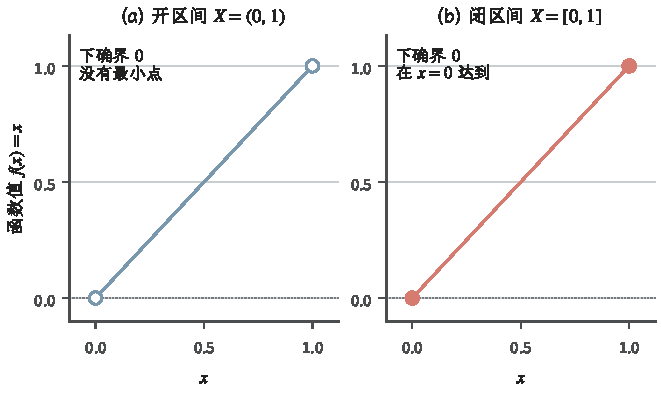
\includegraphics[width=\linewidth]{figures/math-preparation/analysis-concepts/language-minimum-infimum.pdf}
  \caption{同一函数$f(x)=x$的边界对照。左图定义域为$(0,1)$，空心端点不属于图像，函数值可任意接近$0$，却不能取到；右图定义域为$[0,1]$，实心端点$(0,0)$达到下确界。两图的下确界相同，最小点是否存在取决于可行端点是否保留。图为解析教学示例。}
  \label{fig:prelim-minimum-infimum}
\end{figure}

\section{索引族的汇总与递推}
\label{sec:prelim-indices-sums-recurrences}

\subsection{索引族、有限序列与数列}

函数可以把每个索引对应到一个对象，从而保留对象的编号与重复出现。
\begin{definition}[索引族]
\label{def:prelim-indexed-family}
给定索引集合$I$和对象集合$X$，一个索引族是映射$a:I\to X$。
通常把$a(i)$写作$a_i$，整个族写作$(a_i)_{i\in I}$。
\end{definition}
当$I=\{1,\ldots,n\}$并按整数顺序读取时，得到有限序列；当$I$为正整数集时，得到
无限序列，取值为实数时通常称为数列。二维数组则使用索引对$(i,j)$。
索引族允许不同索引对应同一对象，而集合只保留对象是否出现；两者因此不能互相替代。
下面只研究怎样取出、汇总和递推这些对象，数列极限留待分析章。

\subsubsection{索引角色与取值范围}

索引把一族对象排成可引用的形式。本书通常用$i,j,k$标识元素或样本，用$n$表示样本数，
用$d$表示特征维数，用带括号的上标$t$表示迭代步。例如，
$\bm{x}_i\in\mathbb{R}^d$是第$i$个样本，
$x_{i,j}$是该样本的第$j$个坐标，
$\bm{w}^{(t)}$是第$t$次迭代的参数。普通上标则保留给幂：
$w_j^2$表示平方，而$w_j^{(2)}$表示第$2$次迭代中的第$j$个坐标。
若对象本身按时间排列，还应另行声明时间下标，例如$\bm{z}_{\tau}$表示时刻$\tau$的
状态。样本编号、物理时间和算法迭代都可以取整数值，但它们索引的是不同对象，不能仅因
数值相同就互换。

下标只有在取值范围明确时才有意义。把章首的三项有限和推广到$n$项，其中$n$为正整数，得到
\[
  \sum_{i=1}^{n}a_i=a_1+a_2+\cdots+a_n.
\]
其中$i$是求和过程中变化的\term{哑索引}
（dummy index）。把$i$换成$k$不会改变结果。与之不同，等式
\[
  b_j=\sum_{i=1}^{n}x_{i,j}
\]
中的$j$是自由索引：等式对哪些$j$成立需要在附近说明，而且改变$j$会选取不同坐标。
同一个符号不能在一项中既作哑索引又作自由索引。

双重求和需要同时写清两个范围。对有限数组$a_{i,j}$，
\[
  \sum_{i=1}^{n}\sum_{j=1}^{d}a_{i,j}
  =
  \sum_{j=1}^{d}\sum_{i=1}^{n}a_{i,j},
\]
因为两边都遍历同一个有限索引集
$\{1,\ldots,n\}\times\{1,\ldots,d\}$，并把每个索引对$(i,j)$对应的项$a_{i,j}$
恰好相加一次。后文把有限和换成无限级数或积分时，交换次序将需要额外条件，不能直接沿用
这个有限情形的结论。

\subsection{有限和、乘积与加权平均}

有限和中的各项可以先乘系数再相加，也可以先分别求和再乘系数。这来自加法与乘法的
分配律，称为求和的线性关系。对标量$a,b$与同长度序列$(u_i)$、$(v_i)$，
\[
  \sum_{i=1}^{n}(au_i+bv_i)
  =
  a\sum_{i=1}^{n}u_i+b\sum_{i=1}^{n}v_i.
\]
若权重$\alpha_i\geq0$且$\sum_{i=1}^{n}\alpha_i=1$，则
$\sum_i\alpha_i u_i$称为有限\term{加权平均}（weighted average）。
普通样本平均对应$\alpha_i=1/n$。这个简单对象会成为积分与期望的有限版本：积分允许
位置形成连续集合，期望则按概率分配权重。
例如，章首三个平方误差的普通平均是$(1+4+9)/3=14/3$；若权重改为
$1/2$、$1/4$、$1/4$，则加权平均是
$\frac12\cdot1+\frac14\cdot4+\frac14\cdot9=15/4$。两者使用同一组数值，改变的是各项
在汇总结果中的权重。

有限乘积写作$\prod_{i=1}^{n}a_i$。按照空操作不改变结果的约定，
\[
  \sum_{i\in\varnothing}a_i=0,\qquad
  \prod_{i\in\varnothing}a_i=1.
\]
这两个约定分别把$0$和$1$作为加法与乘法的单位元，使递推公式在边界处仍可保持统一。
使用乘积前仍应检查零因子与符号；对正数取对数可把乘积变成和，但含零或负数时不能直接
这样做。

\subsection{递推关系与状态更新}

有限和也可以随着数据到来逐步计算。例如，三个平方误差$1$、$4$、$9$依次到达时，
不必每收到一项就把已有各项重新相加。记$S^{(t)}$为收到前$t$项后的累计值，只需保存
上一轮的累计值，并把新到的一项加进去：
\[
  S^{(0)}=0,\qquad S^{(t+1)}=S^{(t)}+a_{t+1},\qquad t=0,1,2.
\]
在这个例子中，更新依次给出$S^{(1)}=1$、$S^{(2)}=5$、$S^{(3)}=14$。第$t+1$轮只需
知道$S^{(t)}$和新值$a_{t+1}$，而不必保存前$t$项；展开更新则回到
$S^{(t)}=\sum_{i=1}^{t}a_i$。有限和写出累计结果，更新规则写出怎样逐步得到这个结果。

这种从初值出发，用已有项确定后续项的关系称为\term{递推}（recurrence）。对这样的逐步
求值规则，更新规则与初值共同确定序列，只有更新规则通常不能确定每一项。递推也不一定
累加数值：若某种修正
每轮把当前偏差缩小一半，从偏差$8$出发便依次得到$4$、$2$、$1$。用$e^{(t)}$表示
第$t$轮的带符号偏差，把$1/2$推广为固定系数$\rho\in\mathbb{R}$，可写成
\begin{equation}
  e^{(t+1)}=\rho e^{(t)},\qquad e^{(0)}=e_0,\qquad t=0,1,\ldots,
  \label{eq:prelim-geometric-recurrence}
\end{equation}
对整数$t\geq1$逐步展开得到
\[
  e^{(t)}=\rho^t e_0.
\]
对非零初始偏差，$|\rho|<1$使每一步的绝对值缩小，$\rho=-1$使大小不变而符号交替，
$|\rho|>1$使它放大。若$e_0=0$，每一项都是零。这里先由更新规则确定有限步结果；
这些结果在无限多步之后怎样变化，将在分析章讨论。

更一般的误差递推
\begin{equation}
  e^{(t+1)}\leq \rho e^{(t)}+\delta_t,
  \qquad 0\leq\rho<1,
  \label{eq:prelim-perturbed-recurrence}
\end{equation}
包含每一步新加入的非负扰动$\delta_t$，这里将$e^{(t)}$视为非负误差。这个不等式只给出
下一步的误差上界，而不指定它的精确值。再次使用递推不等式，
并利用$\rho\geq0$使不等号方向保持不变，得到
\[
  \begin{aligned}
    e^{(2)}&\leq\rho^2e^{(0)}+\rho\delta_0+\delta_1,\\
    e^{(3)}&\leq\rho^3e^{(0)}+\rho^2\delta_0+\rho\delta_1+\delta_2.
  \end{aligned}
\]
新扰动加入时权重为$1$，此后每经过一轮就再乘一次$\rho$。把这组逐项相加的表达式写成
有限和，对整数$t\geq1$展开$t$步可得
\begin{equation}
  e^{(t)}
  \leq
  \rho^t e^{(0)}
  +
  \sum_{s=0}^{t-1}\rho^{t-1-s}\delta_s.
  \label{eq:prelim-unrolled-recurrence}
\end{equation}
第一项记录初始误差在$t$步后的权重，第二项汇总前$t$步新加入的扰动。
新加入的项经过的更新次数不同，权重也不同；这个有限展开还没有对无限步极限作保证。

式~\eqref{eq:prelim-unrolled-recurrence}可以用数学归纳法证明：先核对$t=1$的基例，再
假设结论对$t$成立并据此推出$t+1$时的结论。完整证明将在本章介绍归纳法时给出。

\section{命题与证明}
\label{sec:prelim-propositions-quantifiers}

对象和计算规则写清之后，还需说明声称了什么：条件在哪些对象上成立，一个选择能依赖
哪些信息，结论要求存在还是唯一。逻辑把这些要求写成真假条件明确的陈述，证明则说明它们
为何由已给条件推出。

\subsection{命题、量词与依赖关系}

\subsubsection{命题与逻辑运算}

\term{命题}（proposition）是在给定语境中具有真假值的陈述。“$F$有最小值”是命题，
“求$F$的最小值”则是任务。带变量的表达式如“$x^2\geq0$”还需要说明$x$的取值范围
或添加量词，才成为完整命题。对实数它成立，对复数若使用通常的序关系则没有定义。

命题$P$的否定记为$\neg P$。两个命题的“且”“或”分别记为
$P\land Q$和$P\lor Q$。数学中的“或”通常是可兼容的：$P$和$Q$同时为真时，
$P\lor Q$仍为真。若只允许恰有一个成立，需要明确写成异或条件。

\term{蕴含}（implication）$P\Rightarrow Q$表示只要$P$为真，$Q$就必须为真。
这里$P$是$Q$的充分条件，$Q$是$P$的必要条件。反向命题$Q\Rightarrow P$需要单独
证明。两向都成立时写作$P\Leftrightarrow Q$，称为等价条件。

定理中的假设正是在限定$P$所覆盖的对象。例如，“目标函数连续且可行域紧致”只允许把
结论用于同时满足这两个条件的问题，不能从定理名称中删去其中一个条件。类似地，“存在
一个最优解”是$\exists x^\star\in X$开头的命题，而“每个初值产生的迭代都收敛”是
$\forall x^{(0)}\in X$开头的另一命题；前者成立并不自动给出后者。

以实数$x$为例，$x>1$是$x^2>1$的充分条件，却不是必要条件，因为$x<-1$时也有
$x^2>1$。条件$x\neq0$是$x^2>0$的充分必要条件。把充分条件误当作必要条件，会排除
本来可能成立的情形；把必要条件误当作充分条件，则可能把不合格对象当成解。

\subsubsection{全称量词与存在量词}

\term{全称量词}（universal quantifier）$\forall$表示“对每一个”，
\term{存在量词}（existential quantifier）$\exists$表示“至少存在一个”。例如
\[
  \forall x\in\mathbb{R},\quad x^2\geq0
\]
是全称命题，而
\[
  \exists x\in\mathbb{R},\quad x^2=2
\]
是存在命题。存在并不表示唯一；要表达恰有一个对象满足条件，可以写
$\exists!x$，但使用时仍应说明存在性与唯一性各由什么保证。

否定量词时，量词种类与内部命题同时改变：
\begin{align*}
  \neg\bigl(\forall x\in X,\ P(x)\bigr)
  &\Longleftrightarrow
  \exists x\in X,\ \neg P(x),\\
  \neg\bigl(\exists x\in X,\ P(x)\bigr)
  &\Longleftrightarrow
  \forall x\in X,\ \neg P(x).
\end{align*}
所以，要推翻“每个输入都满足性质$P$”，找到一个不满足的输入即可；要证明“没有输入
满足$P$”，则必须排除所有输入。

\subsubsection{量词次序与依赖关系}

考虑样本集合$S=\{1,\ldots,n\}$和参数集合$W$，令$C(w,i)$表示参数$w$在第$i$个
样本上预测正确。陈述
\begin{equation}
  \exists w\in W,\quad \forall i\in S,\quad C(w,i)
  \label{eq:prelim-one-parameter-all-samples}
\end{equation}
要求找到同一个参数，使它对所有样本都正确。陈述
\begin{equation}
  \forall i\in S,\quad \exists w\in W,\quad C(w,i)
  \label{eq:prelim-each-sample-some-parameter}
\end{equation}
却允许参数随样本改变，因而弱得多。

\begin{example}[逐点可选不等于统一可选]
\label{ex:prelim-quantifier-order}
令$S=W=\{0,1\}$，并规定$C(w,i)$当且仅当$w=i$。对每个$i$，选择$w=i$即可，
所以式~\eqref{eq:prelim-each-sample-some-parameter}成立。但不存在一个$w$同时等于
$0$和$1$，所以式~\eqref{eq:prelim-one-parameter-all-samples}不成立。
\end{example}

\begin{table}[htbp]
 \centering\small
 \begin{tabularx}{\linewidth}{@{}lccX@{}}
 \toprule
 参数 & 样本$0$ & 样本$1$ & 对量词的含义\\
 \midrule
 $w=0$ & 成立 & 不成立 & 不能覆盖全部样本\\
 $w=1$ & 不成立 & 成立 & 不能覆盖全部样本\\
 \bottomrule
 \end{tabularx}
 \caption{例~\ref{ex:prelim-quantifier-order}的条件真值。每一列都有一个可选参数，却没有一行同时成立。}
 \label{tab:prelim-quantifier-truth-pattern}
\end{table}

例~\ref{ex:prelim-quantifier-order}说明，量词次序改变了允许依赖哪些信息。
统计学习中的“对每个允许分布，以高概率得到小误差”也包含多个量词；算法、样本量和
失败概率是否可以依赖分布，必须由量词位置决定，不能靠自然语言猜测。

\subsection{公式模型与逻辑后承}

\subsubsection{赋值、子句与满足}


把逻辑连接词作用于有限个命题变量，便得到\term{布尔公式}（Boolean formula）。
变量各取什么值是一件事，整个公式是否成立是另一件事；为了检验规则，需要把这两层对象
明确区分。蕴含也可以写成一个不允许反例的析取式：
\begin{equation}
  P\Rightarrow Q\quad\Longleftrightarrow\quad\neg P\lor Q.
  \label{eq:comb-implication-clause}
\end{equation}

\begin{definition}[赋值与公式的模型]
\label{def:comb-assignment-model}
给定命题变量$z_1,\ldots,z_n$，\term{赋值}（assignment）是映射
$\nu:\{z_1,\ldots,z_n\}\to\{\mathrm{false},\mathrm{true}\}$；连接词的真值规则
递归地确定$\nu$是否满足一个公式。满足公式$\Phi$的赋值也称为$\Phi$的
\term{模型}（model），全体模型记为$\operatorname{Mod}(\Phi)$。
\end{definition}
这个“模型”只指
逻辑公式的满足赋值，不等同于后续章节中由参数描述的统计模型。

否定复合命题时，De Morgan律给出
\begin{equation}
  \neg(P\land Q)\Longleftrightarrow(\neg P\lor\neg Q),
  \qquad
  \neg(P\lor Q)\Longleftrightarrow(\neg P\land\neg Q).
  \label{eq:comb-de-morgan}
\end{equation}
以第一式为例，$(P,Q)$依次取$(0,0),(0,1),(1,0),(1,1)$时，等式两侧的真值都依次为
$1,1,1,0$；第二式同理得到$1,0,0,0$。逐行相同证明两边具有相同模型集合，而不是
仅在某个选定赋值上碰巧相等。

为把多条规则写在一起，需要区分规则中的基本真假项与一条完整要求。
\begin{definition}[文字、子句与合取范式]
\label{def:comb-literals-cnf}
一个文字是命题变量$z_i$或它的否定$\neg z_i$；一个子句是若干文字的析取，
只要其中至少一个文字为真，该子句就为真。若公式由若干子句合取而成，就称为
\term{合取范式}（conjunctive normal form, CNF），它要求所有子句同时为真。
\end{definition}

取四个候选$V_0=\{1,2,3,4\}$，用$z_i$表示“候选$i$被选择”，真与假分别记作$1$与$0$。
要求候选$1$与$2$恰选一个，候选$3$被选时必须选$1$，候选$4$被选时必须选$2$或$3$。
这些规则可以写成
\begin{equation}
  \Phi(\bm{z})
  =
  (z_1\lor z_2)
  \land(\neg z_1\lor\neg z_2)
  \land(\neg z_3\lor z_1)
  \land(\neg z_4\lor z_2\lor z_3).
  \label{eq:comb-running-cnf}
\end{equation}
前两个子句共同表达$z_1,z_2$恰有一个为真；第三个子句表达
$z_3\Rightarrow z_1$；第四个子句表达$z_4\Rightarrow(z_2\lor z_3)$。


\begin{definition}[满足、可满足与永真]
\label{def:comb-satisfiability}
赋值$\bm{z}$若使$\Phi(\bm{z})$为真，就称它\term{满足}（satisfy）$\Phi$。
至少存在一个满足赋值时，公式\term{可满足}（satisfiable）；不存在时称为不可满足。
这里要判断的是
\[
  \exists\bm{z}\in\{0,1\}^n,\quad \Phi(\bm{z})=\mathrm{true},
\]
不是证明$\Phi$对每个赋值都真。对每个赋值都真的公式称为永真式；可满足性与永真性
对应不同的量词，不能混用。
\end{definition}

例如，赋值$(1,0,0,0)$与$(0,1,0,1)$都满足这组规则，
$(1,1,0,0)$却违反前两个候选的互斥要求。第~\ref{chap:combinatorics}章将把模型
写成候选集合，研究模型数量、寻找模型的程序及其代价；这里先检验陈述的真假含义。

\subsubsection{后承、多个模型与冲突}

一个可行答案只说明一组规则不矛盾；要判断另一条结论是否被规则强制，还需检查所有可行答案。
\begin{definition}[逻辑后承]
\label{def:comb-logical-consequence}
若每个满足$\Phi$的赋值也满足命题$\Psi$，记作
\[
  \Phi\models\Psi,
\]
称$\Psi$是$\Phi$的\term{逻辑后承}（logical consequence）。
\end{definition}
这表示规则已经强制
推出$\Psi$，不表示某个求解器碰巧返回了满足$\Psi$的一个答案。例如，由
式~\eqref{eq:comb-running-cnf}可得
\[
  \Phi\models(z_3\Rightarrow\neg z_2),
\]
因为$z_3$推出$z_1$，而$z_1$与$z_2$互斥。还可得
\[
  \Phi\land z_4\land\neg z_2
  \models z_3\land z_1.
\]
后一结论使用了额外观测$z_4=1,z_2=0$，不能去掉这些条件后仍声称
$\Phi\models z_3$。用真变量的下标集合表示一个模型，$\Phi\land z_4\land\neg z_2$只有
$\{1,3,4\}$这一个模型；原公式$\Phi$则有五个模型。这组规则因此同时给出了唯一答案、
多个答案与下段冲突情形的可复核对照。

规则允许多个模型时，可满足性只确认“至少有一个答案”。$\{1\}$与$\{2,4\}$都满足
$\Phi$，所以规则本身没有在二者之间作出选择。若再加入$z_2$与$z_3$这两个只含一个文字的单位子句，
公式变为不可满足：$z_3$推出$z_1$，却又要求互斥的$z_2$为真。冲突表示全部硬规则
无法同时成立，不等于程序尚未找到答案。

判断$\Phi\models\Psi$可以转化为一次不可满足性检查：
\begin{equation}
  \Phi\models\Psi
  \quad\Longleftrightarrow\quad
  \Phi\land\neg\Psi\text{ 不可满足}.
  \label{eq:comb-entailment-unsat}
\end{equation}
若右侧可满足，其模型就是一个满足$\Phi$却违反$\Psi$的反例；若右侧不可满足，
这样的反例不存在。这个等价关系把全称式的逻辑后承转换为存在反例的搜索。

定义还包含一个容易误读的边界：若$\Phi$本身不可满足，则
$\operatorname{Mod}(\Phi)=\varnothing$，因而对任意$\Psi$都有
$\Phi\models\Psi$。这称为空真，并不表示冲突规则提供了关于$\Psi$的有效信息。
实际推理通常先检查$\Phi$可满足，再解释它的逻辑后承。

\subsection{证明形式与合法反例}
\label{sec:prelim-proofs-constructions-counterexamples}

同一个结论可以用不同方式论证，选择哪一种取决于已知条件能怎样发挥作用。本节用几个
短例子比较这些方式：蕴含命题可以从条件推到结论，也可以排除结论不成立的情形；存在
命题可以给出满足条件的对象；由整数索引的一族命题则可以利用相邻项之间的递推关系。
反例承担另一项任务：找出一个满足前提却违反结论的对象，以说明某个全称命题不成立。

\subsubsection{直接证明、逆否证明与反证法}

证明不是把若干正确公式排列在一起，而是从已给条件出发，经过每一步都合法的推理到达
结论。开始证明前，先辨认命题的逻辑形式。对$P\Rightarrow Q$，直接证明从$P$出发；
逆否证明改证$\neg Q\Rightarrow\neg P$；反证法假设$P$成立而$Q$不成立，并推出矛盾。
这些形式在逻辑上等价，但哪一种更清楚取决于条件怎样进入计算\scite{math-graham1994concrete}

下面用最小点的唯一性说明反证法怎样工作。最小点是允许范围内没有更小函数值的点；要
排除两个不同的最小点，可以反设它们存在，再构造一个函数值更小的允许点。

\begin{example}[用反证法排除两个最小点]
\label{ex:prelim-strict-midpoint-unique-minimizer}
设$C\subseteq\mathbb{R}^d$满足：任取$\bm{u},\bm{v}\in C$，其中点
$(\bm{u}+\bm{v})/2$仍属于$C$。若函数$F:C\to\mathbb{R}$对任意不同的
$\bm{u},\bm{v}\in C$都满足
\begin{equation}
  F\left(\frac{\bm{u}+\bm{v}}{2}\right)
  <
  \frac{F(\bm{u})+F(\bm{v})}{2},
  \label{eq:prelim-strict-midpoint-condition}
\end{equation}
那么$F$在$C$上至多有一个最小点。

中点条件提供了构造更小函数值的办法。反设
$\bm{u}\neq\bm{v}$都是最小点，并把共同的最小值记为$m$。由$C$对取中点封闭，
$(\bm{u}+\bm{v})/2\in C$。再由式~\eqref{eq:prelim-strict-midpoint-condition}，
\[
  F\left(\frac{\bm{u}+\bm{v}}{2}\right)
  <
  \frac{m+m}{2}
  =m.
\]
这与$m$是最小值矛盾，所以不可能存在两个不同的最小点。
例如，$F(x)=x^2$在$\mathbb{R}$上满足这一条件，因为
\[
  \frac{u^2+v^2}{2}-\left(\frac{u+v}{2}\right)^2
  =\frac{(u-v)^2}{4}>0\qquad(u\neq v).
\]
这里不是逐个检查所有候选点，而是说明任意两个不同的候选最小点都会与同一个条件冲突。
\end{example}

例~\ref{ex:prelim-strict-midpoint-unique-minimizer}只证明“至多一个”，没有证明
最小点存在。函数可以满足排除两个最小点的条件，却根本没有最小点。第~\ref{chap:optimization}
章会把中点条件扩展为凸性，并分别建立存在条件与唯一条件。

\subsubsection{构造性证明}

存在命题$\exists x\in X,\ P(x)$可以通过构造一个具体$x$并核对$P(x)$来证明。
例如，要证明对任意$a,b\in\mathbb{R}$且$a<b$，存在$c$满足$a<c<b$，可以取
$c=(a+b)/2$。由$a<b$分别加上$a$与$b$，再除以正数$2$，得到
\[
  a<\frac{a+b}{2}<b.
\]
构造不仅说明对象存在，还可能给出计算它的方法。

但存在性与可构造性不是同一个逻辑要求。某些证明通过排除“不存在”的可能来确认对象存在，
却不提供有限步骤找到该对象。反过来，一个算法给出候选对象，也仍要证明它终止并满足条件。
后文谈“最优解存在”和“算法收敛”时，会分别承担这两项责任。

\subsubsection{数学归纳法}

数学归纳法适合证明由整数$n$索引的一族命题$P(n)$。它包括基例和归纳步：先证明
$P(n_0)$，再证明对每个$n\geq n_0$，$P(n)$蕴含$P(n+1)$。这两步共同覆盖所有
$n\geq n_0$，不能只展示几个数值例子。

回到式~\eqref{eq:prelim-unrolled-recurrence}，它对每个整数$t\geq1$给出同一种误差界，
正适合用归纳法验证。
\begin{proof}[式~\eqref{eq:prelim-unrolled-recurrence}的归纳证明]
当$t=1$时，式~\eqref{eq:prelim-perturbed-recurrence}正是所需结论。假设结论对$t$成立，
再使用一次递推式，得到
\begin{align*}
  e^{(t+1)}
  &\leq \rho e^{(t)}+\delta_t\\
  &\leq
  \rho^{t+1}e^{(0)}
  +
  \sum_{s=0}^{t-1}\rho^{t-s}\delta_s
  +\delta_t\\
  &=
  \rho^{t+1}e^{(0)}
  +
  \sum_{s=0}^{t}\rho^{t-s}\delta_s.
\end{align*}
这就是把$t$换成$t+1$后的式子，归纳完成。
\end{proof}

同样的归纳结构还可以验证熟悉的有限和公式。关键在于把第$n+1$项单独分离，让剩下的
$n$项恰好由归纳假设控制。

\begin{example}[用归纳法计算前$n$个正整数之和]
\label{ex:prelim-arithmetic-sum}
对每个$n\in\mathbb{N}$且$n\geq1$，
\[
  \sum_{i=1}^{n}i=\frac{n(n+1)}{2}.
\]
当$n=1$时，两边都等于$1$。假设公式对某个$n\geq1$成立，则
\[
  \sum_{i=1}^{n+1}i
  =
  \left(\sum_{i=1}^{n}i\right)+(n+1)
  =
  \frac{n(n+1)}{2}+(n+1)
  =
  \frac{(n+1)(n+2)}{2}.
\]
这正是$n+1$时的公式，故结论对所有$n\geq1$成立。
例如$n=4$时，$1+2+3+4=10=4\cdot5/2$；这个数值核对只是展示公式的含义，覆盖所有
正整数的是基例与归纳步共同构成的论证。
\end{example}

归纳假设只能用于已经假设的$P(n)$，不能把待证的$P(n+1)$换一种说法后当作依据。
若递推依赖前两个状态，则归纳假设和基例也要覆盖相应数量的前项。

\subsubsection{反例与适用边界}

一个全称命题声称所有允许对象都满足某种性质，所以一个合法反例就足以推翻它。反例必须
满足原命题的前提而违反结论；若它同时违反前提，只能说明例子不在讨论范围内。

例如，“目标函数有下界就一定达到最小值”是错误的。取
\[
  X=(0,1),\qquad f(x)=x.
\]
$f(x)>0$，所以$0$是下界；而对每个$x\in(0,1)$，$x/2$仍在$(0,1)$中且
$f(x/2)<f(x)$，所以没有任何$x$达到最小值。失败原因不是函数不连续，而是定义域没有
包含趋近边界时的极限点。第~\ref{chap:mathematical-analysis}章会用闭性、紧致性和连续性
给出保证极值达到的条件。

反例也能区分相近概念。一个参数化不是单射，说明参数未必可识别；它不说明预测函数一定
不能确定。一次迭代使目标下降，说明当前步骤有效；它不说明所有迭代都会收敛到全局最优。
把结论限制到证据真正覆盖的对象，是证明工作的一部分。

\section{本章小结}
\label{sec:prelim-sets-functions-summary}

数学表达同时规定对象、范围、条件和保证。集合与关系说明对象怎样取值、分类和比较，
函数区分输入、输出与参数化选择；下确界属于函数取值的边界，最小点则要求某个合法输入
实际取得这个边界。参数是否能由完整函数辨认，又是映射是否单射的问题。

索引族保留编号、顺序和重复，有限和汇总各项，递推由初值和更新规则确定后续项。
有限展开能说明指定步数的结果，不能代替无限过程的收敛论证。命题、模型与量词进一步
写清哪些条件必须同时成立，以及选择允许依赖哪些信息；存在不等于唯一，一个满足赋值
也不能代替对全部模型的后承保证。构造、归纳和反例分别回应不同形式的论证要求。

接下来的第~\ref{chap:combinatorics}章用这些语言研究候选空间、求解任务与程序，
第~\ref{chap:mathematical-analysis}章则研究极限、连续变化与累计量。
在使用这些工具之前，仍须先辨认结论讨论哪个对象、覆盖什么范围，以及所需保证是什么。

\chapter{计数与计算}
\label{chap:combinatorics}

第~\ref{chap:sets-functions-and-proofs}章已建立集合、函数、索引族与逻辑陈述的语言。
现在考察离散对象的结果空间，以及对这些对象提出的求解任务。
同样一组候选，可以问有多少种不同结果、哪些结果满足规则、哪一个目标值最好；还可以
问是否存在处理所有合法输入的统一程序，以及程序需要多少资源。这些问题相互关联，
但结果数量不能直接给出必需的枚举成本，模式容量也不能代替算法复杂度。

本章用二值选择说明它们的分工。对非负整数$n$，令
\[
  V=\{1,\ldots,n\},\qquad
  \bm z=(z_i)_{i\in V}\in\{0,1\}^n,\qquad
  S(\bm z)=\{i\in V:z_i=1\}.
\]
赋值与子集是同一选择的两种表示。在贯穿例子中记$V_0=\{1,2,3,4\}$，
回用前章式~\eqref{eq:comb-running-cnf}的四候选规则：
候选$1$与$2$恰选一个，候选$3$依赖$1$，候选$4$要求$2$或$3$至少出现一个。
集合计数研究这些表示的数量和贡献结构；函数族限制到有限输入后，则得到可计数的标记模式。
规则与目标随后定义判定、搜索和优化任务，程序理论再对整类输入讨论可计算能力与资源。
最后一种考察不限于这个小例子，也不限于有限候选的枚举。

\section{候选空间的结构与计数}
\label{sec:comb-families-counting}

数量比较必须固定结果对象：一个有序选择、一个子集和一个输入上的标记模式，不能混用
同一种计数口径。以下先建立精确计数及增长尺度，再分别处理重叠校正、局部贡献恢复和
函数族的模式容量；这些结论刻画结果空间，不预先断言求解程序必须怎样运行。

\subsection{集合族与候选规模}

第~\ref{chap:sets-functions-and-proofs}章已经区分集合、序列和索引族。计数时还要
确定哪些表示属于同一个结果，再研究规则改变后候选数量怎样变化。一个\term{集合族}（set family）
$\mathcal{F}\subseteq\mathcal{P}(V)$是一组允许讨论的子集。若不加任何限制，
$\mathcal{F}=\mathcal{P}(V)$；各元素选择与否不受其他元素约束，所以
\begin{equation}
  |\mathcal{P}(V)|=2^n.
  \label{eq:comb-power-set-count}
\end{equation}

候选由若干选择组成时，需要知道共有多少种不同结果。计数时必须先确定，交换选择次序是否得到同一个对象。
设$n,k$为整数且$0\leq k\leq n$。从$n$个不同对象中依次取出$k$个且不放回，
若顺序重要，可得到
\[
  P(n,k)=n(n-1)\cdots(n-k+1)=\frac{n!}{(n-k)!}
\]
种排列。若只关心选中了哪些对象，不关心次序，每个大小为$k$的子集被计算了$k!$次，
因此组合数为
\begin{equation}
  \binom{n}{k}=\frac{n!}{k!(n-k)!},
  \qquad 0\leq k\leq n.
  \label{eq:prelim-binomial-coefficient}
\end{equation}
规定$\binom{n}{k}=0$用于$k<0$或$k>n$，可以统一许多边界公式。

把$n$个对象的子集按是否包含某个固定对象分组，可得Pascal恒等式
\[
  \binom{n}{k}
  =
  \binom{n-1}{k}
  +
  \binom{n-1}{k-1}.
\]
第一项计算不包含固定对象的子集，第二项先包含该对象，再从其余$n-1$个对象中选择
$k-1$个。这种“为同一集合建立不重不漏的两种计数”称为组合证明。下面的容斥与子集反演会继续利用这种有限分组与抵消的思路。

二项式定理把组合数与代数展开连接起来：
\begin{equation}
  (a+b)^n
  =
  \sum_{k=0}^{n}\binom{n}{k}a^k b^{n-k}.
  \label{eq:prelim-binomial-theorem}
\end{equation}
选择展开式中的一项时，需要从$n$个因子中挑出$k$个贡献$a$，其余贡献$b$，所以
$a^k b^{n-k}$前的系数正是$\binom{n}{k}$。概率论中的二项分布和学习理论中的有限类
计数都会复用这个关系。

例如，从$\{1,2,3,4\}$中取两个元素有$12$个有序对，却只有$6$个二元子集；
$(1,3)$与$(3,1)$在前一个任务中不同，在后一个任务中表示同一个结果。

幂集的数量也可按子集大小分层计算，再由二项式定理得到
$\sum_{k=0}^{n}\binom{n}{k}=(1+1)^n=2^n$。二值选择与按大小分层是两种计数口径，
计算的是同一批子集。

每个$S\subseteq V$也确定一个有序二分划分$(S,V\setminus S)$，所以有序二分划分
仍有$2^n$个。若两部分没有名称，$(S,V\setminus S)$与$(V\setminus S,S)$表示
同一个划分；当$n\geq1$时没有子集等于自己的补集，每个无序划分恰被计算两次，数量为
$2^{n-1}$。是否区分两侧决定了计数对象，不能只看它们都把$V$分成两部分。
这里允许某一部分为空；若要求两部分都非空，有序与无序数量应分别减为
$2^n-2$与$2^{n-1}-1$。当$n=0$时，交换两侧不会产生两个不同表示，上述除以$2$的
论证也不适用。

若只允许恰好选择$k$项，集合族变为
\[
  \binom{V}{k}=\{S\subseteq V:|S|=k\},
  \qquad
  \left|\binom{V}{k}\right|=\binom{n}{k}.
\]
若允许至多选择$k$项，则数量为$\sum_{j=0}^{k}\binom{n}{j}$。因此“候选总数有限”
仍可能掩盖完全不同的增长规模：固定$k$时，该和关于$n$至多按$n^k$增长；
$k$随$n$线性增长时，候选数却可能接近$2^n$。

计数常可通过一个变量把问题拆成两个较小问题。记$a_{n,k}$为从$n$个元素中选择
$k$个的方案数。对$n\geq1$，固定元素$n$后，所有方案被不重不漏地分成“不含$n$”
与“含$n$”两类。为使边界项也有定义，约定$a_{0,0}=1$，并在$k<0$或$k>n$时令
$a_{n,k}=0$。于是对$n\geq1$和任意整数$k$都有
\begin{equation}
  a_{n,k}=a_{n-1,k}+a_{n-1,k-1}.
  \label{eq:comb-binomial-recurrence}
\end{equation}
这既是Pascal恒等式，也是一个递推算法。

\subsection{计数与代价的增长尺度}
\label{sec:comb-growth-scales}

候选数量与算法成本都可能随输入规模变化，精确值不同的两个序列也可能具有同一增长尺度。设$a_n$与$b_n$为实数序列，且从某个位置开始
$b_n>0$。若存在常数$C>0$和$n_0$，使得
\[
  \forall n\geq n_0,\qquad |a_n|\leq Cb_n,
\]
则记$a_n=O(b_n)$。这表示$a_n$的绝对值最终被$b_n$的常数倍控制，常数$C$不随$n$
改变。若对任意$\varepsilon>0$，都存在$n_\varepsilon$使
\[
  \forall n\geq n_\varepsilon,\qquad |a_n|\leq\varepsilon b_n,
\]
则记$a_n=o(b_n)$。这要求最终能用任意小的正比例控制$a_n$，比一个固定常数倍的界更强。
第~\ref{chap:mathematical-analysis}章会把它表述为比值趋于零，并用于函数的局部余项。

例如$n=O(n)$、$3n+7=O(n)$且$\log n=o(n)$。但大O不是精确等式：
$n=O(n^2)$也成立，只是界较松。写算法复杂度时还要说明被计数的操作、输入规模和计算
模型；写统计误差时则要说明界是确定性的、期望意义的还是以高概率成立
\scite{math-graham1994concrete}

当序列还依赖维数$d$或其他规模时，也要说明哪些量允许进入隐含常数。例如，对每个固定
$d$都有$d/n=O(1/n)$，因为可以取$C=d$；但若要求同一个$C$同时适用于任意$d$，这个
界就不成立。因此，“关于$n$是某个速率”不等于该速率对维数一致。需要一致结论时，应把
量词写成对所讨论的全部$d$使用同一组$C$与$n_0$，或把$d$显式保留在界中。

对迭代序列，常用$t$而不是$n$表示步数。若目标$F:\mathbb{R}^d\to\mathbb{R}$
有有限下确界，记$F^\star=\inf_{\bm{w}\in\mathbb{R}^d}F(\bm{w})$；达到它的
参照最小点（若存在）记为$\bm{w}^\star$。例如
\[
  F(\bm{w}^{(t)})-F^\star=O(1/t)
\]
表示存在与$t$无关的常数控制目标值误差。这个式子没有说明参数误差
$\lVert\bm{w}^{(t)}-\bm{w}^\star\rVert_2$具有同样速率，也没有说明一次迭代的成本。
比较算法时，必须固定误差对象和成本口径。

前一小节的组合数递推也可以按这个口径评估。
若只保存上一行，计算全部
$a_{n,0},\ldots,a_{n,n}$需要$O(n^2)$次加法和$O(n)$个存储单元。
闭式公式、递推关系和计算过程由此承担不同作用：闭式便于分析规模，递推揭示分组结构，
算法还必须说明求值顺序和资源。

\subsection{容斥原理与重复计数}

直接把若干坏情形的数量相加会重复计算同时违反多条规则的赋值。
\term{容斥原理}（inclusion--exclusion principle）用交集项逐层校正这种重复。

\begin{theorem}[有限容斥原理]
\label{thm:comb-inclusion-exclusion}
设$A_1,\ldots,A_m$是有限集合。则
\begin{equation}
  \left|\bigcup_{i=1}^{m}A_i\right|
  =
  \sum_{\varnothing\neq I\subseteq\{1,\ldots,m\}}
  (-1)^{|I|+1}
  \left|\bigcap_{i\in I}A_i\right|.
  \label{eq:comb-inclusion-exclusion}
\end{equation}
\end{theorem}

\begin{proof}
固定任意元素$x$，设它恰好属于$r$个集合。若$r=0$，它在等式两侧都没有贡献。
若$r\geq1$，右侧从含有$x$的$r$个集合中选择非空索引集，给$x$计算的总系数为
\[
  \sum_{k=1}^{r}(-1)^{k+1}\binom{r}{k}
  =
  1-\sum_{k=0}^{r}(-1)^k\binom{r}{k}
  =1-(1-1)^r=1.
\]
所以并集中的每个元素在右侧恰好被计算一次，对所有$x$求和即得结论。
\end{proof}

回到$V_0$上的四个变量。把三条规则的违反事件记为
\[
  \begin{aligned}
    A_1&=\{\bm{z}:z_1=z_2\},\\
    A_2&=\{\bm{z}:z_3=1,\ z_1=0\},\\
    A_3&=\{\bm{z}:z_4=1,\ z_2=0,\ z_3=0\}.
  \end{aligned}
\]
它们分别表示基础标签没有恰选一个、缺少候选$1$时仍选择候选$3$，以及候选$4$缺少前提。
全部赋值有$16$个，并且
\[
  |A_1|=8,\quad |A_2|=4,\quad |A_3|=2.
\]
交集大小为
\[
  |A_1\cap A_2|=2,\qquad
  |A_1\cap A_3|=1,\qquad
  |A_2\cap A_3|=|A_1\cap A_2\cap A_3|=0.
\]
由式~\eqref{eq:comb-inclusion-exclusion}，坏赋值共有
$8+4+2-2-1=11$个，因此可行赋值有$16-11=5$个。它们对应
\begin{equation}
  \mathcal{C}_0
  =
  \bigl\{
  \{1\},\{1,3\},\{1,3,4\},\{2\},\{2,4\}
  \bigr\}.
  \label{eq:comb-running-feasible-family}
\end{equation}
这些集合恰是前章式~\eqref{eq:comb-running-cnf}的全部模型。
第~\ref{sec:comb-logic-constraints}节将区分检查、判定与搜索对这批对象所要求的回答。

\subsection{子集格上的 Möbius 反演}

容斥处理的是若干集合的重叠。一个更一般的问题是：若已知每个$S$上的总量由其全部
子集贡献累加而成，能否还原每个子集自身新增的贡献？子集按包含关系形成前章定义的偏序。两个子集的交是包含于两者的最大子集，
并则是包含两者的最小子集；这种带有交、并运算的子集偏序称为子集格。
\term{Möbius反演}（Möbius inversion）给出这一累加变换的逆。

\begin{theorem}[子集格上的 Möbius 反演]
\label{thm:comb-mobius-inversion}
设$g,h:\mathcal{P}(V)\to\mathbb{R}$满足
\begin{equation}
  g(S)=\sum_{T\subseteq S}h(T)
  \qquad\text{对每个 }S\subseteq V.
  \label{eq:comb-zeta-transform}
\end{equation}
则
\begin{equation}
  h(S)
  =
  \sum_{T\subseteq S}(-1)^{|S|-|T|}g(T).
  \label{eq:comb-mobius-inversion}
\end{equation}
反过来，由式~\eqref{eq:comb-mobius-inversion}定义$h$也会恢复
式~\eqref{eq:comb-zeta-transform}。
\end{theorem}

更一般的有限偏序集把$T\subseteq S$换成$T\preceq S$。其Möbius函数由
$\mu(S,S)=1$以及
$\mu(T,S)=-\sum_{T\preceq R\prec S}\mu(T,R)$（$T\prec S$）递归确定，
不满足$T\preceq S$时取$\mu(T,S)=0$。反演系数不再只由
$|S|-|T|$决定。本章只使用子集格，此时递归解恰为
$\mu(T,S)=(-1)^{|S|-|T|}$。

\begin{proof}
把式~\eqref{eq:comb-zeta-transform}代入反演式右侧并交换有限求和次序，得到
\begin{align*}
  \sum_{T\subseteq S}(-1)^{|S|-|T|}g(T)
  &=
  \sum_{T\subseteq S}(-1)^{|S|-|T|}
  \sum_{R\subseteq T}h(R)\\
  &=
  \sum_{R\subseteq S}h(R)
  \sum_{T:R\subseteq T\subseteq S}
  (-1)^{|S|-|T|}.
\end{align*}
固定$R$后，中间集合$T$由$S\setminus R$中哪些元素被加入决定。若
$q=|S\setminus R|$，内层和等于
\[
  \sum_{j=0}^{q}\binom{q}{j}(-1)^{q-j}
  =(1-1)^q.
\]
它在$R=S$时为$1$，在$R\neq S$时为$0$，所以全部较小子集的贡献抵消，只留下
$h(S)$。同一抵消关系也证明反向代入恢复$g$。
\end{proof}

在小集合$V_0$上，假设累计得分具有形式
\[
  g(S)
  =
  2|S|
  +3\mathbb{I}\{\{1,3\}\subseteq S\}
  -\mathbb{I}\{\{2,4\}\subseteq S\}.
\]
每个单项贡献$2$，组合$\{1,3\}$额外贡献$3$，而组合$\{2,4\}$产生$-1$的交互。
四个元素共有$16$个子集。把每个子集的累计值与反演恢复的局部贡献并列，可以完整核对
正向累加与反向消去：
\begin{table}[htbp]
  \centering
  \caption{四元素子集格上的累计值与局部贡献。除四个单项、交互
  $\{1,3\}$和$\{2,4\}$外，其余局部贡献均为零。}
  \label{tab:comb-four-element-mobius}
  \begin{tabular}{ccc@{\qquad}ccc}
    \toprule
    $S$ & $g(S)$ & $h(S)$ & $S$ & $g(S)$ & $h(S)$ \\
    \midrule
    $\varnothing$ & $0$ & $0$ & $\{1,2\}$ & $4$ & $0$ \\
    $\{1\}$ & $2$ & $2$ & $\{1,3\}$ & $7$ & $3$ \\
    $\{2\}$ & $2$ & $2$ & $\{1,4\}$ & $4$ & $0$ \\
    $\{3\}$ & $2$ & $2$ & $\{2,3\}$ & $4$ & $0$ \\
    $\{4\}$ & $2$ & $2$ & $\{2,4\}$ & $3$ & $-1$ \\
    $\{3,4\}$ & $4$ & $0$ & $\{1,2,3\}$ & $9$ & $0$ \\
    $\{1,2,4\}$ & $5$ & $0$ & $\{1,3,4\}$ & $9$ & $0$ \\
    $\{2,3,4\}$ & $5$ & $0$ & $V_0$ & $10$ & $0$ \\
    \bottomrule
  \end{tabular}
\end{table}
若只观察各子集的累计值，反演给出
\[
  h(\{i\})=g(\{i\})-g(\varnothing)=2,
\]
以及
\[
  \begin{aligned}
  h(\{1,3\})
  &=g(\{1,3\})-g(\{1\})-g(\{3\})+g(\varnothing)=3,\\
  h(\{2,4\})
  &=g(\{2,4\})-g(\{2\})-g(\{4\})+g(\varnothing)=-1.
  \end{aligned}
\]
其余大小至少为$2$的局部贡献均为零。反演并没有假设贡献为正；它只保证累计量与局部
交互之间可以互相重构。

例如对$S=\{1,2,3\}$，累计值为$g(S)=9$，三个二元子集的累计值依次为
$4,7,4$，三个单元素累计值之和为$6$，且$g(\varnothing)=0$。反演确实给出
\[
  h(\{1,2,3\})=9-(4+7+4)+6-0=0.
\]
把已经恢复的单项贡献$2,2,2$与二元贡献$3$重新相加，也得到
$g(\{1,2,3\})=9$。正向累加与反向消去由此可以在同一组数值上相互复核。

图~\ref{fig:comb-mobius-cumulative-local}只保留$\{1,3\}$的四个子集，比较累计量与局部量。
累计值$g(\{1,3\})=7$包括两个单项的$2$以及共同出现才增加的$3$；反演消去两个单项后，
留下的是交互贡献$3$，并不是把累计值本身改成负数或丢掉较小子集。
\begin{figure}[htbp]
 \centering
 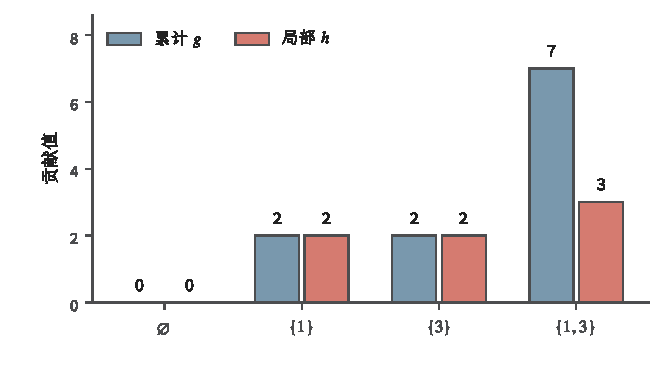
\includegraphics[width=\linewidth]{figures/math-preparation/reader-revision-analysis/combinatorics-mobius-cumulative-local.pdf}
 \caption{同一四元素教学构造在$\{1,3\}$的子集上的累计值与局部贡献。蓝柱为$g$，红柱为$h$；
 单项贡献各为$2$，二元累计值$7$包含额外交互$3$。图中四个子集的数据由正文解析式精确计算，
 没有省略影响这个二元交互的子集。}
 \label{fig:comb-mobius-cumulative-local}
\end{figure}

容斥原理可以看成同一反演机制作用于指示函数。正负号
$(-1)^{|S|-|T|}$不是需要另行记忆的巧合，而是“所有严格更小子集相互抵消”所需的系数。
后续图模型会把这一重构用于变量子集间的局部交互，再用图结构限制哪些交互允许出现。
Möbius反演本身只是一条有限集合恒等式，不会自动给出这些结构限制，也不保证所得局部项非负。

\subsection{二值函数族的标记模式与容量}
\label{sec:comb-label-family-capacity}

集合族的计数固定了已给出的候选规则。函数类的比较还要允许输入点改变，
并控制任意有限输入组上能实现多少种输出模式。把标记向量看作集合后，
同样的递推计数可建立VC维与多类别维度的界；实值输出则用阈值与间隔区分数值选择。
这里研究的是模式丰富度，
统计误差还需概率条件，求解代价还需程序与编码；模式容量本身不能回答这两类问题。

\subsubsection{限制类与可实现标记}

无限函数类在有限输入上只留下有限个二值标记。这里把每种标记改写成一个子集，再用能够实现多少种模式来刻画它的组合丰富度；第~\ref{chap:probability-theory}章则把这种有限化用于同时误差控制。
给定输入$x_1,\ldots,x_m$和二值函数类$\mathcal{H}$，每个$h\in\mathcal{H}$确定
\[
  A_h=\{i\in\{1,\ldots,m\}:h(x_i)=1\}.
\]
函数在这组输入上的标记向量与$A_h$一一对应，因此不同标记的数量就是集合族
$\{A_h:h\in\mathcal{H}\}\subseteq\mathcal{P}(\{1,\ldots,m\})$的大小。式~
\eqref{eq:comb-power-set-count}随即给出上界$2^m$；生长函数只是在所有输入组中取这个
数量的上确界。

下列定义针对非空输入空间上的非空二值函数类
\(\mathcal H\subseteq\{0,1\}^{\mathcal X}\)，不涉及抽样分布。
把输入集\(C=\{x_1,\ldots,x_m\}\)按所列次序排列，在\(C\)上的限制类
记录这组输入上全部可实现的标记向量：
\[
  \mathcal H|_C=\{(h(x_1),\ldots,h(x_m)):h\in\mathcal H\}.
\]
\begin{definition}[打散]
  \label{def:shattering}
  若对有限互异输入集\(C\)的每个二值标记\((b_1,\ldots,b_m)\)，都存在\(h\in\mathcal H\)满足\(h(x_i)=b_i\)对全部\(i\)成立，就称\(\mathcal H\)\term{打散}（shatter）\(C\)。等价地，\(\mathcal H|_C=\{0,1\}^m\)。
\end{definition}
\begin{definition}[VC维]
  \label{def:vc-dimension}
  \(\mathcal H\)的\term{VC维}（Vapnik--Chervonenkis dimension）为
  \[
    \operatorname{VC}(\mathcal H)
    =\sup\{|C|:C\subseteq\mathcal X,\ |C|<\infty,\ C\text{被}\mathcal H\text{打散}\}.
  \]
  空集总能被非空函数类打散，所以维度可为\(0\)；若任意大有限集都能被打散，则取值为\(+\infty\)。
\end{definition}
\begin{definition}[生长函数]
  \label{def:growth-function}
  对整数\(m\geq0\)，定义
  \begin{equation}
    \Pi_{\mathcal H}(m)
    =\max_{x_1,\ldots,x_m\in\mathcal X}
    |\{(h(x_1),\ldots,h(x_m)):h\in\mathcal H\}|.
    \label{eq:growth-function}
  \end{equation}
  \(m=0\)时只有一个空标记，故\(\Pi_{\mathcal H}(0)=1\)。
\end{definition}
VC维记录可完整实现全部模式的最大输入集大小；生长函数记录任意给定输入数下最多实现多少模式。输入可重复的约定使有限输入空间上的式~\eqref{eq:growth-function}也对全部\(m\)有定义；重复输入不会产生新的独立标记位。

这个表示还能直接计算受基数约束的函数族。令$\mathcal{X}$为无限集，固定$k\geq0$，并设
\[
  \mathcal{H}_k
  =
  \{h_S:S\subseteq\mathcal{X},\ |S|\leq k\},
  \qquad
  h_S(x)=\mathbb{I}\{x\in S\}.
\]
对$m$个互异输入，$\mathcal{H}_k$能够实现的正类索引集合恰是所有大小不超过$k$的
子集，因而
\[
  \Pi_{\mathcal{H}_k}(m)
  =
  \sum_{j=0}^{\min\{k,m\}}\binom{m}{j}.
\]
固定$k$时，这个数量关于$m$至多按$m^k$增长；当$k\geq m$时，它恢复为$2^m$。
同一个幂集计数由此区分出多项式规模与指数规模。它仍只描述有限输入上的模式数，
不直接给出统计误差界，也不保证能够高效找到实现某种标记的函数。

一个可逐项复核的例子是实数轴上的区间分类器。令
$x_1<\cdots<x_m$互异，函数$h_{a,b}(x)=\mathbb{I}\{a\leq x\leq b\}$把落在某个
闭区间内的输入标为$1$。非空正类索引必为连续块
$\{i,i+1,\ldots,j\}$，这样的块由$1\leq i\leq j\leq m$唯一确定；再加上空正类，
可实现模式数恰为
\[
  1+\sum_{i=1}^{m}(m-i+1)
  =
  1+\frac{m(m+1)}2.
\]
当$m=3$时，七个模式为$000,100,010,001,110,011,111$，只有$101$无法实现。
因此三个有序点不能被该函数类打散；两个点的四种模式都能实现。这个算例也说明，
参数$a,b$取值无限多，并不意味着有限输入上的标记模式也有无限多个。

图~\ref{fig:comb-interval-shattering-patterns}把“每一种模式”逐项展开。两个点的四种标记
都能由一个区间实现；三个点的$101$要求包含两端却排除中点，违背区间的连续块结构。
图~\ref{fig:combinatorics-growth-patterns}随后只保留模式数量，两张图分别回答实现结构与增长规模。
\begin{figure}[htbp]
 \centering
 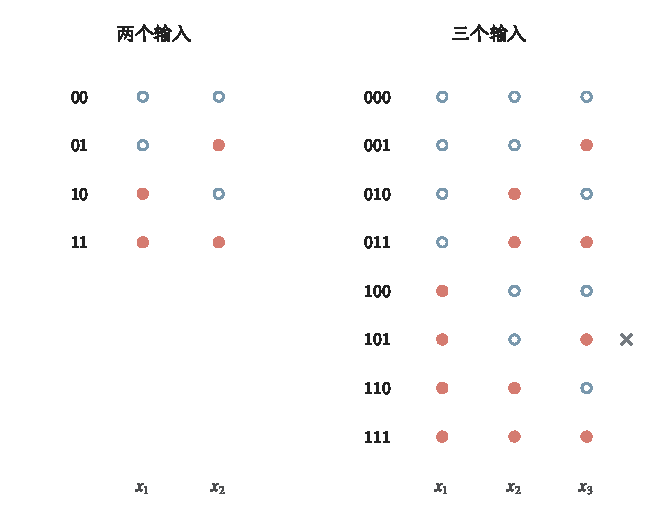
\includegraphics[width=\linewidth]{figures/math-preparation/reader-revision-analysis/combinatorics-interval-shattering-patterns.pdf}
 \caption{区间分类器在互异有序输入上的全部二值模式。红实心点表示标记$1$，蓝空心点表示标记$0$；
 每行是一种模式。左侧两个输入的四行全部可实现，右侧三个输入仅$101$不可实现，灰色叉号标出缺失行。
 这是精确的有限模式构造，不是抽样统计。}
 \label{fig:comb-interval-shattering-patterns}
\end{figure}

图~\ref{fig:combinatorics-growth-patterns}把区间类与全部标记放在对数轴上比较。区间类的两个端点参数虽有无穷多种取值，有限输入上的模式数却仅按平方增长。计数相同也不表示函数类相同：当\(k=2\)时，\(\mathcal H_k\)的模式数同样为\(1+m(m+1)/2\)，但在三个点上它缺少\(111\)，区间类却缺少\(101\)。因此生长函数约束丰富程度，并不完整记录模式的结构。

\begin{figure}[htbp]
  \centering
  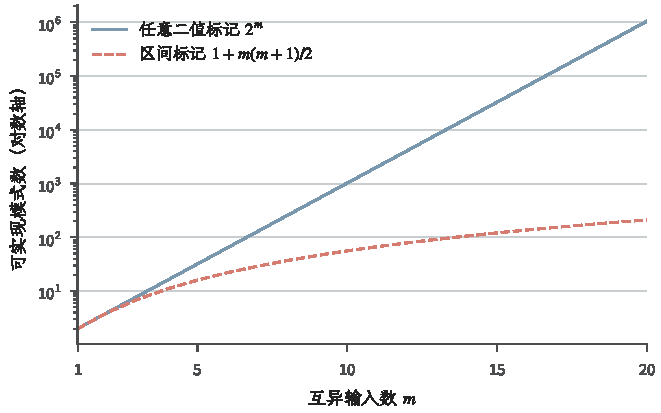
\includegraphics[width=\linewidth]{figures/math-preparation/probability-discrete/combinatorics-growth-patterns.pdf}
  \caption{有限输入上的二值模式数（精确计数教学图）。蓝实线为不受限制的\(2^m\)，红虚线为实数轴区间分类器的\(1+m(m+1)/2\)。纵轴使用对数刻度，红线是该具体类的精确计数；它也恰等于至多两个正类点的集合族计数，但两类实现的模式可以不同。}
  \label{fig:combinatorics-growth-patterns}
\end{figure}

\subsubsection{VC维与Sauer--Shelah计数界}
\label{sec:comb-vc-growth}

区间例子的VC维为\(2\)，而模式数恰好达到\(1+m+\binom m2\)。下面的计数界解释为何有限VC维足以限制全部输入上的增长，证明复用式~\eqref{eq:comb-binomial-recurrence}的“最后一个坐标”分组，但需要同时记录哪些旧模式能够接上两个不同标签。
\begin{lemma}[Sauer--Shelah引理]
  \label{lem:sauer-shelah}
  若\(d=\operatorname{VC}(\mathcal H)<\infty\)，则对任意\(m\geq0\)，
  \[
    \Pi_{\mathcal H}(m)\leq\sum_{j=0}^{\min\{d,m\}}\binom mj.
  \]
  特别地，当\(1\leq d\leq m\)时，
  \begin{equation}
    \Pi_{\mathcal H}(m)\leq\sum_{j=0}^{d}\binom mj
    \leq\left(\frac{em}{d}\right)^d.
    \label{eq:sauer-shelah}
  \end{equation}
\end{lemma}
\begin{proof}
固定\(m\)个输入上的有限模式族\(\mathcal A\subseteq\{0,1\}^m\)。令\(U\)为删去末坐标后的所有模式，\(V\subseteq U\)为既能接\(0\)又能接\(1\)的模式，则
\( |\mathcal A|=|U|+|V|\)。\(U\)不能打散超过\(d\)个坐标。\(V\)也不能打散\(d\)个坐标，否则在这些坐标上任意赋值，再把末坐标任意取\(0\)或\(1\)，就会由\(\mathcal A\)打散\(d+1\)个坐标，产生矛盾。

对坐标数归纳。零坐标时至多一个模式；\(d=0\)时也至多一个模式，因为两个不同模式在某一坐标取值不同，便会打散一个坐标。对\(m,d\geq1\)，归纳假设和上面的分组给出
\[
  |\mathcal A|
  \leq\sum_{j=0}^{d}\binom{m-1}{j}
       +\sum_{j=0}^{d-1}\binom{m-1}{j}
  =\sum_{j=0}^{d}\binom mj,
\]
其中超过坐标数的组合数约定为零。重复输入不会增大模式数，因此对全部输入组取最大值得到第一项结论。

当\(1\leq d\leq m\)时，令\(a=d/m\in(0,1]\)。对\(j\leq d\)有\(a^d\leq a^j\)，故
\[
  a^d\sum_{j=0}^{d}\binom mj
  \leq\sum_{j=0}^{d}\binom mj a^j
  \leq(1+a)^m\leq e^{am}=e^d.
\]
除以\(a^d\)便得到简化界。\(d=0\)时第一项界为\(1\)，不使用含\(d\)作分母的简化式。
\end{proof}
引理只给出计数，不直接给出概率保证，也不保证能高效找到实现某种标记的函数。固定\(d\)后，计数上界至多按\(m^d\)增长；具体类可以更慢。要控制经验平均，还需第~\ref{chap:probability-theory}章中的抽样、可测性和集中条件。

\subsection{多类别标记族的组合维度}
\label{sec:comb-multiclass-dimensions}

两个标签时，每个点只有一种与当前标签不同的选择；三个以上标签时，“改为另一个标签”却不唯一。例如两个输入上的六个模式
\[
  \mathcal V=\{(a,a),(a,b),(b,b),(b,c),(c,c),(c,a)\}
\]
没有包含任何固定两标签对的四角矩形，但每个模式都能只改变任一坐标而仍留在\(\mathcal V\)中。完整二元立方体与局部逐坐标歧义不再是同一条件，需要把所允许的标签选择写进定义。

图~\ref{fig:comb-multiclass-pattern-grid}把这个有限例子放进两坐标表格。沿一行移动
只改变第二个标签，沿一列移动只改变第一个标签；每个实心点都能沿两种方向找到另一个
实心点，但没有任取两行两列形成的四个角同时占满。局部可改变与完整二选一组合由此
可以直接区分。
\begin{figure}[htbp]
 \centering
 \figurefont\footnotesize\color{FigureInk}
 \renewcommand{\arraystretch}{1.6}
 \begin{tabular}{cccc}
 \toprule
 第一坐标$\backslash$第二坐标 & $a$ & $b$ & $c$\\
 \midrule
 $a$ & $\bullet$ & $\bullet$ & $\circ$\\
 $b$ & $\circ$ & $\bullet$ & $\bullet$\\
 $c$ & $\bullet$ & $\circ$ & $\bullet$\\
 \bottomrule
 \end{tabular}
 \caption{六模式族$\mathcal V$的精确占位图。实心点表示模式属于该族，空心点表示缺失模式。每行每列恰有两个实心点，却没有完整的四角矩形；这不是两个标签的完整立方体。}
 \label{fig:comb-multiclass-pattern-grid}
\end{figure}

本小节设\(\mathcal H\subseteq Y^X\)非空，\(X,Y\)为非空集合。有限点集中的输入均互异，\(\mathcal H|_C\)依固定的输入次序写成标记向量。以下维度均取可打散有限集大小的上确界，允许\(0\)与\(+\infty\)。

\begin{definition}[Natarajan打散与Natarajan维]
\label{def:natarajan-dimension}
设$C=\{x_1,\ldots,x_m\}\subseteq X$。若存在$f,g:C\to Y$，满足
$f(x)\neq g(x)$对所有$x\in C$成立，且对每个$B\subseteq C$都存在$h_B\in\mathcal H$使
\begin{equation}
 h_B(x)=\begin{cases}f(x),&x\in B,\\g(x),&x\in C\setminus B,\end{cases}
 \label{eq:natarajan-shattering}
\end{equation}
则称$C$被$\mathcal H$ \term{Natarajan打散}（Natarajan shattering）。令$\mathcal C_N$为所有被
$\mathcal H$ Natarajan打散的有限输入集组成的集合，定义
\[
 d_N(\mathcal H)=\sup_{C\in\mathcal C_N}|C|.
\]
\end{definition}

\begin{definition}[图打散]
\label{def:graph-dimension}
若有限集$C\subseteq X$存在$f:C\to Y$，使每个$B\subseteq C$都对应某个
$h_B\in\mathcal H$，满足
\[
 h_B(x)=f(x)\ (x\in B),\qquad h_B(x)\neq f(x)\ (x\in C\setminus B),
\]
则称$C$被$\mathcal H$图打散。
\end{definition}

\begin{definition}[图维]
\label{def:graph-dimension-value}
设$\mathcal C_G$为所有被$\mathcal H$图打散的有限输入集组成的集合，定义
\[
 d_G(\mathcal H)=\sup_{C\in\mathcal C_G}|C|.
\]
\end{definition}

Natarajan打散固定了每个输入上的两个候选标签，图打散只固定一个基准标签；偏离基准时具体采用哪个标签可以随子集改变。为了描述前面六模式例子中的局部邻接，还需一个不预先固定标签对的对象。

\begin{definition}[伪立方体]
\label{def:pseudocube}
有限非空集合$V\subseteq Y^m$称为$m$维伪立方体，如果对每个$v\in V$和
每个$i\in\{1,\ldots,m\}$，都存在$u\in V$满足
$u_i\neq v_i$且$u_j=v_j$对所有$j\neq i$成立。
\end{definition}

\begin{definition}[DS维]
\label{def:ds-dimension}
若$m$个互异输入组成的有序点集$C$满足$\mathcal H|_C$包含一个$m$维伪立方体，
则称$C$被\term{DS打散}（DS shattering）。DS维$d_{DS}(\mathcal H)$定义为可被
DS打散的有限点集大小的上确界。
\end{definition}

伪立方体要求\(V\)有限、非空，并对其中每个模式的每个坐标都能找到邻居；只在一个起始模式附近有邻居并不够。邻居只改变一个坐标，却不要求整个族共享某两种标签。

\begin{table}[htbp]
  \centering
  \caption{多类别组合维度的不同量词。图维中的“图”指标记相等关系的图打散，不是输入关系图的顶点数。}
  \label{tab:comb-multiclass-dimensions}
  \begin{tabular}{p{0.17\linewidth}p{0.70\linewidth}}
    \toprule
    维度 & 在有限输入上的要求\\
    \midrule
    Natarajan维 & 每点固定两个不同标签，全部\(2^m\)种逐点二选一组合均可实现\\
    图维 & 每点固定一个基准标签，任意点集上匹配、其补集上不匹配的模式均可实现\\
    DS维 & 包含有限非空模式族，每个模式在任一坐标都可单独改变并仍留在族中\\
    \bottomrule
  \end{tabular}
\end{table}
\subsubsection{有限标签的计数界}

维度描述能够实现的局部选择，生长函数则计算全部标记模式。要把两者联系起来，先将
式~\eqref{eq:growth-function}中的二值函数类换成\(\mathcal H\subseteq Y^X\)：
固定\(m\)个输入后，计算\(\mathcal H\)在这些输入上产生的不同标记向量，再对全部
输入组取最大值。有限标签时这个数量至多为\(|Y|^m\)，最大值存在；允许重复输入的
约定使有限输入空间也能讨论任意\(m\)。继续用\(\Pi_{\mathcal H}(m)\)表示这个生长函数。
Natarajan维限制每个坐标上固定两标签的独立选择，因而可以沿用Sauer--Shelah引理的
计数思路。不过，一个前缀现在可能接上两个以上标签，递推必须计入所有不同标签对。

\begin{theorem}[有限标签的预测数目上界]
\label{thm:multiclass-growth-bound}
设\(2\leq |Y|=K<\infty\)，\(d=d_N(\mathcal H)<\infty\)。
记\(q=\binom K2=K(K-1)/2\)为不同无序标签对的数目，则对每个整数\(m\geq0\)，
\begin{equation}
  \Pi_{\mathcal H}(m)\leq G_{d,K}(m)
  :=\sum_{j=0}^{\min\{d,m\}}\binom mj q^j.
  \label{eq:comb-multiclass-growth-bound}
\end{equation}
\end{theorem}

\begin{proof}
将有限非空模式族\(V\subseteq Y^m\)视为坐标集\(\{1,\ldots,m\}\)上的函数类，
并设其Natarajan维至多为\(d\)。删去末坐标得到前缀族\(U\subseteq Y^{m-1}\)。
对\(u\in U\)，记它能够接上的末尾标签数为\(r(u)\geq1\)。这个前缀对\(|V|\)
贡献\(r(u)\)，对\(|U|\)贡献\(1\)；多出的\(r(u)-1\)不超过它能够接上的标签对数
\(\binom{r(u)}2\)。对每个不同标签对\(\{a,b\}\)，令\(U_{a,b}\)为既能接上\(a\)
又能接上\(b\)的前缀族。对前缀求和可得
\[
  |V|\leq |U|+\sum_{\substack{\{a,b\}\subseteq Y\\a\neq b}}|U_{a,b}|.
\]
每个无序对在求和中只出现一次。\(U\)的Natarajan维至多为\(d\)。当\(d\geq1\)
时，每个非空\(U_{a,b}\)的Natarajan维至多为\(d-1\)：否则它可以在某\(d\)个
坐标上实现全部固定标签对的选择；每个对应前缀又能接上\(a\)或\(b\)，使\(V\)
在这\(d\)个坐标与末坐标上实现全部二元选择，违反维度上界。空\(U_{a,b}\)的
计数贡献为零。

记\(M(m,d)\)为Natarajan维至多\(d\)的非空模式族\(V\subseteq Y^m\)能够达到的
最大大小，标签集\(Y\)保持固定。对\(m,d\geq1\)，上述分组给出
\[
  M(m,d)\leq M(m-1,d)+qM(m-1,d-1).
\]
零个坐标只有一个空模式，故\(M(0,d)=1\)。维度为零时也至多有一个模式：两个
不同模式必在某坐标上取不同标签，从而Natarajan打散一个坐标。因此\(M(m,0)=1\)。
对\(m\)归纳，将两个较小问题的上界代入，并使用二项式递推关系，得到
\[
\begin{aligned}
  M(m,d)
  &\leq\sum_{j=0}^{d}\binom{m-1}{j}q^j
       +q\sum_{j=0}^{d-1}\binom{m-1}{j}q^j\\
  &=\sum_{j=0}^{d}\binom mj q^j,
\end{aligned}
\]
其中超出坐标数的组合数约定为零。任意输入组上的限制类，其Natarajan维不超过
\(d_N(\mathcal H)\)；重复输入不能作为两个可独立选择的坐标。因此对输入组取最大值，
得到式~\eqref{eq:comb-multiclass-growth-bound}。
\end{proof}

当\(K=2\)时，\(q=1\)，该求和式恢复为引理~\ref{lem:sauer-shelah}的二值计数界。
多出的\(q^j\)记录参与选择的\(j\)个坐标还可以使用不同标签对，而不表示一个具体
函数类一定能达到上界。例如，\(K=3\)、\(d=1\)、\(m=4\)时，上界为
\(1+4\times3=13\)，小于无约束的\(3^4=81\)。固定\(d,K\)后，这个上界关于
\(m\)至多按多项式增长；将模式数用于统计学习时，还需另加抽样与概率条件。

\subsubsection{组合维度的比较}

表~\ref{tab:comb-multiclass-dimensions}中的量词不同，却有一条共同的包含关系。
固定两标签的完整选择产生伪立方体；伪立方体中的逐坐标邻居又能够实现相对某个基准
模式的任意匹配与偏离。计数界还说明：标签数有限时，有限Natarajan维不允许图打散
任意大的输入集，因为图打散需要指数多个不同模式。

\begin{theorem}[多分类维度的比较]
\label{thm:multiclass-dimension-comparison}
对任意非空标签空间与非空函数类，有
\[
  d_N(\mathcal H)\leq d_{DS}(\mathcal H)\leq d_G(\mathcal H).
\]
二标签时三者均等于VC维。若\(|Y|=K<\infty\)，则\(d_N(\mathcal H)<\infty\)
也蕴含\(d_G(\mathcal H)<\infty\)。
\end{theorem}

\begin{proof}
若\(m\)个输入被Natarajan打散，每个坐标的两个候选标签固定，全部\(2^m\)种
选择组成一个有限非空模式族。任意模式都能只翻转任一坐标上的选择并仍留在族中，
所以它是\(m\)维伪立方体，证明\(d_N\leq d_{DS}\)。

若限制类包含\(m\)维伪立方体\(V\)，固定\(v\in V\)作为基准。任取希望偏离基准
的坐标集\(I\subseteq\{1,\ldots,m\}\)，逐个沿\(I\)中的坐标移动到邻居，每个
坐标只移动一次。每一步仅改变当前坐标；之前改变的坐标保持不变，\(I\)之外的
坐标始终与\(v\)相同。因此最终模式恰在\(I\)上不等于\(v\)，在其补集上等于
\(v\)。令\(I\)遍历所有子集就得到图打散，故\(d_{DS}\leq d_G\)。

二标签时，偏离基准的标签唯一。图打散因此要求全部二元模式；伪立方体从任意模式
逐坐标翻转也能到达全部二元模式。Natarajan打散中的两标签正是整个标签集，所以
三种维度都等于VC维。

若\(K=1\)，函数类在任何输入上只有一种标记，三种维度均为零。若\(2\leq K<\infty\)
且\(d_N=d<\infty\)，图打散\(m\)个输入至少需要\(2^m\)个不同模式。由定理~
\ref{thm:multiclass-growth-bound}，必有\(2^m\leq G_{d,K}(m)\)。固定\(d,K\)后，
右侧至多按多项式增长，左侧按指数增长，故能够被图打散的\(m\)有有限上界。
\end{proof}

前面的\(\mathcal V\)每行和每列都恰有两个模式，所以构成二维伪立方体。它没有四角矩形，故不能Natarajan打散两个输入，而至少能打散一个，得到\(d_N=1\)。以\((a,a)\)为基准，\((a,a),(a,b),(c,a),(b,b)\)分别实现两个坐标上全匹配、仅第一坐标匹配、仅第二坐标匹配、均不匹配，因而\(d_G=2\)，并有\(d_{DS}=2\)。这是有限模式族的精确组合例子；它本身不构成不可学习性证明，相关统计条件由机器学习理论部分另行讨论。

\subsection{实值函数的阈值与间隔}
\label{sec:comb-real-valued-threshold-margins}

前面的多类别维度把标签视为不同的符号。实值输出还具有大小关系，可以用阈值把
数值变化转成高低模式；阈值必须在检验全部模式之前固定。例如两个输入处以$20$为
阈值，四种高低组合都可实现，便表示两处数值可以独立跨过阈值。这里沿用固定有限
输入与实现全部二元选择的组合结构，新增的是输出的大小关系及两侧的间隔要求。
本小节取非空输入空间上的非空函数类$\mathcal F$，有限输入$x_1,\ldots,x_m$互异；
阈值可以随这些输入选定，却不能在看到待实现模式后重新选择。

\begin{definition}[伪打散]
\label{def:pseudo-shattering}
设$\mathcal F\subseteq\mathbb R^{\mathcal X}$。有限集$C=\{x_1,\ldots,x_m\}$被
$\mathcal F$\term{伪打散}（pseudo-shattering），是指存在$r_1,\ldots,r_m\in\mathbb R$，使任意
$\bm b\in\{0,1\}^m$都对应某个$f_{\bm b}\in\mathcal F$，满足
\[
 b_i=1\Rightarrow f_{\bm b}(x_i)>r_i,\qquad
 b_i=0\Rightarrow f_{\bm b}(x_i)<r_i\quad(1\leq i\leq m).
\]
\end{definition}
\begin{definition}[伪维]
\label{def:pseudo-dimension}
$\mathcal F$的\term{伪维}（pseudo-dimension）为
$\operatorname{Pdim}(\mathcal F)=\sup\{|C|:C\text{为被}\mathcal F\text{伪打散的有限集}\}$，
允许值为$+\infty$；没有非空被打散集合时值为$0$。
\end{definition}

二值类取阈值$1/2$后，伪打散与VC打散一致，故其伪维等于VC维。实值类则仍缺少尺度：
$20.001$和$19.999$已处于阈值两侧，却未必能在精度为$1$的观测中分辨。
\term{胖打散}（fat-shattering）要求每一侧再留出宽度$\gamma$的间隔。

\begin{definition}[胖打散]
\label{def:fat-shattering}
给定$\gamma>0$，若有限集$C=\{x_1,\ldots,x_m\}$存在固定阈值$r_1,\ldots,r_m$，
使任意$\bm b\in\{0,1\}^m$均对应$f_{\bm b}\in\mathcal F$满足
\begin{equation}
 b_i=1\Rightarrow f_{\bm b}(x_i)\geq r_i+\gamma,\qquad
 b_i=0\Rightarrow f_{\bm b}(x_i)\leq r_i-\gamma,
 \label{eq:fat-shattering}
\end{equation}
则称$C$在尺度$\gamma$下被$\mathcal F$胖打散。
等价地，以$\sigma_i=2b_i-1$编码，可写为
\begin{equation}
 \sigma_i\bigl(f_{\bm\sigma}(x_i)-r_i\bigr)\geq\gamma
 \quad(i=1,\ldots,m).
 \label{eq:functional-fat-shattering}
\end{equation}
\end{definition}
\begin{definition}[胖打散维]
\label{def:fat-shattering-dimension}
尺度$\gamma$下的\term{胖打散维}（fat-shattering dimension）为
$\operatorname{fat}_\gamma(\mathcal F)=
\sup\{|C|:C\text{为在尺度}\gamma\text{下被}\mathcal F\text{胖打散的有限集}\}$。
采用与伪维相同的$0$及$+\infty$约定。
\end{definition}

$\gamma$增大时，允许的模式只会减少，胖打散维因此单调不增。伪维计算能否跨过阈值，
胖打散维进一步计算能否以规定幅度跨过阈值；两者不能由参数个数直接代替。

幅度约束怎样进入这个维数，可以用分块常值函数直接算出。
\begin{example}[分块常值函数的胖打散维]
\label{ex:comb-piecewise-constant-fat-dimension}
设非空集合$A_1,\ldots,A_m$构成$\mathcal{X}$的一个划分，并令
\[
  \mathcal{F}_B
  =
  \left\{
    \sum_{j=1}^{m}a_j\mathbb{I}_{A_j}:
    |a_j|\leq B
  \right\},
  \qquad B>0.
\]
当$0<\gamma\leq B$时，从每个$A_j$选一点并取阈值$r_j=0$；对任意符号模式令
$a_j=\gamma\sigma_j$，便能以间隔$\gamma$实现该模式，所以这$m$个点被胖打散。反过来，
任意$m+1$个点中至少两个落在同一个$A_j$内，而类中每个函数在这两个点取值相同。若二者
的阈值为$r$与$r'$且能够被胖打散，模式$(+1,-1)$要求$r'-r\geq2\gamma$，模式
$(-1,+1)$又要求$r-r'\geq2\gamma$，二者矛盾。因此该尺度下的胖打散维恰为$m$。
当$\gamma>B$时，
单点上的两个符号也要求函数值之差至少为$2\gamma$，超过允许区间$[-B,B]$的宽度$2B$，
故胖打散维为$0$。这个算例把分区数控制的自由方向与系数上界控制的可分辨幅度分开了。
\end{example}

图~\ref{fig:comb-fat-margin-output-square}把例~\ref{ex:comb-piecewise-constant-fat-dimension}
中的两个分块写成输出平面。系数上界限定一个正方形；胖打散还要求四种高低选择分别跨过
固定阈值两侧的间隔。间隔增大到超过系数范围后，候选函数仍然存在，只是再也无法满足这些选择要求。
\begin{figure*}[htbp]
 \centering
 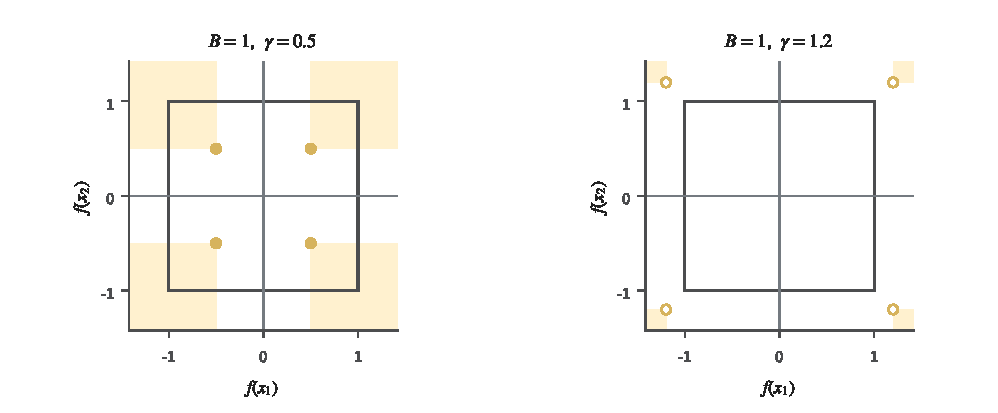
\includegraphics[width=\linewidth]{figures/math-preparation/reader-revision-analysis/combinatorics-fat-margin-output-square.pdf}
 \caption{两个分块、$B=1$与固定阈值$r_1=r_2=0$的输出几何。灰框是函数类允许的
 $(f(x_1),f(x_2))\in[-1,1]^2$；浅黄区域要求两坐标分别离阈值至少$\gamma$。
 左图$\gamma=0.5$的四种符号可由实心点实现；右图$\gamma=1.2$的空心点只标出要求的边界，
 全部落在允许框之外，因而不是类中的函数输出。图为解析教学构造。}
 \label{fig:comb-fat-margin-output-square}
\end{figure*}

组合维度回答函数类能实现哪些模式；一个给定的标记或选择向量是否符合任务约束，
则需要下一节的逻辑规则。

\section{候选空间上的约束与求解}
\label{sec:comb-constrained-solving}

同一个候选空间可以承载不同的任务：规则决定答案是否允许，目标决定允许答案之间怎样
比较，算法保证则说明返回结果的质量。这里回用前章的逻辑语义，明确判定、搜索和优化的
输入输出；随后考察覆盖结构和扩大候选范围分别能给出什么保证。

\subsection{规则系统的判定与搜索任务}
\label{sec:comb-logic-constraints}

第~\ref{chap:sets-functions-and-proofs}章已定义公式的赋值、模型与逻辑后承。
现在把规则作为程序的输入：检查一个给定赋值是否满足、回答有没有满足赋值，以及在有解时
返回一个赋值，是三个不同的任务。前者只检验一个对象，后两者需要处理整个候选空间。

\term{布尔可满足性问题}（Boolean satisfiability problem, SAT）的输入是一个布尔
公式，输出只回答它是否存在满足赋值。输入限制为CNF时称为CNF-SAT；进一步要求每个
子句至多含三个文字时称为\term{3-SAT}。若采用“恰含三个文字”的定义，可以重复文字
补齐较短的非空子句，不改变可满足性；输入若含空子句，则公式立即不可满足。
式~\eqref{eq:comb-running-cnf}因此既是一个CNF-SAT
实例，也是一个3-SAT实例。三者共享“是否存在满足赋值”这一判定接口，但允许的输入
语法不同，不能只凭名称互换实例。

这里回用式~\eqref{eq:comb-running-cnf}的四变量规则。它的模型可以写成
$S(\bm z)=\{i:z_i=1\}$，全部模型恰组成式~\eqref{eq:comb-running-feasible-family}的
五个集合。容斥计算模型数量，SAT只回答是否至少有一个；搜索程序还需实际输出见证。
逻辑后承也可由式~\eqref{eq:comb-entailment-unsat}转为查找反模型，仍须区别语义上的
等价关系与执行这次查找的程序代价。

\subsubsection{逻辑子句与零一约束}

布尔规则也可以写成关于$z_i\in\{0,1\}$的代数约束。一个文字若为$z_i$，
用数值$z_i$表示；若为$\neg z_i$，用$1-z_i$表示。子句
$\ell_1\lor\cdots\lor\ell_r$恰好等价于
\begin{equation}
  \sum_{j=1}^{r}v(\ell_j)\geq1,
  \qquad
  v(z_i)=z_i,\quad v(\neg z_i)=1-z_i.
  \label{eq:comb-clause-linearization}
\end{equation}
因为左侧计算为真的文字个数，至少一个文字为真当且仅当该和不小于$1$。

式~\eqref{eq:comb-running-cnf}因而等价于
\begin{equation}
  z_1+z_2=1,\qquad
  z_3\leq z_1,\qquad
  z_4\leq z_2+z_3,\qquad
  \bm{z}\in\{0,1\}^4.
  \label{eq:comb-running-integer-constraints}
\end{equation}
第一条等式同时包含“至少一个”和“至多一个”。这些条件给出了前章所说的可行域，
其中变量的零一取值条件必须保留。后续第~\ref{chap:optimization}章会进一步研究
可行域的几何结构与求解条件。

若把$\bm{z}\in\{0,1\}^4$放宽为$\bm{z}\in[0,1]^4$，就允许了更多数值候选，
得到一个连续松弛。
分数点
\[
  \bm{z}=(1/2,1/2,1/2,1)
\]
满足全部松弛约束，却不是任何逻辑赋值。按阈值$1/2$把各坐标都取为$1$，还会违反
$z_1+z_2=1$。松弛点可提供优化界或帮助构造整数解，但它本身不是规则系统的合法答案；
取整后必须重新核对原约束。

\subsection{可行选择的目标与近似保证}
\label{sec:comb-optimization-submodularity}

逻辑规则确定哪些集合允许，但通常仍会留下多个答案。
现在给每个可行集合一个数值目标，选择其中最优者；次模性限制增加元素时的边际收益，
从而为贪心近似提供结构保证。计数、可行性和目标值分别属于候选规模、规则与偏好，
不能用其中一项代替另外两项。

\subsubsection{硬规则与偏好代价}

\begin{definition}[硬约束]
\label{def:comb-hard-constraint}
给定候选集合$Z$与必须满足的条件$\phi_1,\ldots,\phi_m$，\term{硬约束}
（hard constraint）把可行集合限定为
$\mathcal C=\{\bm z\in Z:\phi_j(\bm z)\text{为真，对所有}j\}$。
违反任意一条的对象不属于可行集合。
\end{definition}
有些规则表达偏好而非绝对禁止，此时可以为违反规则设置非负代价。令
$r_j(\bm{z})\in\{0,1\}$表示第$j$条规则是否被违反，权重$\lambda_j\geq0$，
则可以最小化
\begin{equation}
  c(\bm{z})+\sum_{j=1}^{m}\lambda_j r_j(\bm{z}),
  \qquad
  \bm{z}\in\{0,1\}^n.
  \label{eq:comb-soft-constraint-objective}
\end{equation}
$c$是任务本身的代价，第二项为规则冲突计分。权重有限时，足够大的任务收益可能抵消
违反规则的代价，所以软规则不再具有逻辑蕴含意义。

把$\lambda_j$取得很大也不能未经证明就等同于硬约束。若$c$的变化范围已知，例如
$|c(\bm{z})-c(\bm{z}')|\leq B$对任意赋值成立，并且存在一个不违反任何软规则的
赋值$\bm{z}_0$，那么令每个$\lambda_j>B$可以排除所有带违反项的全局最优解：
任一违规赋值的目标值严格大于$c(\bm{z}_0)$。若不存在零违反赋值、无法给出可用的
$B$，或希望一族不同规模的实例共用罚权而$c$的振幅没有统一上界，或者只把部分权重
取得较大，这个论证便不成立。
若还为违规程度引入额外变量，同样要说明它们允许哪些原本被排除的赋值。
这些做法各自改变了可行性或比较准则，使用时应明确允许返回什么答案。

\subsubsection{最优解与近似质量}

规则确定集合族$\mathcal{C}\subseteq\mathcal{P}(V)$后，仍需用目标函数比较不同
可行集合。一个有限组合优化问题可写成
\begin{equation}
  \max_{S\in\mathcal{C}}F(S)
  \qquad\text{或}\qquad
  \min_{S\in\mathcal{C}}C(S).
  \label{eq:comb-discrete-optimization}
\end{equation}
由于$\mathcal{C}$有限且非空，实值目标一定达到最优值。这只回答存在性；验证
$S\in\mathcal{C}$、计算$F(S)$以及在不枚举全部候选的情况下找到最优解，仍是不同任务。
存在性的证明只需把$\mathcal{C}=\{S_1,\ldots,S_N\}$列成有限序列：有限个实数
$F(S_1),\ldots,F(S_N)$可逐项比较并取得最大值，达到该值的某个$S_i$就是最优解。
最小化结论可对$-C$应用同一论证。
若$\mathcal{C}=\varnothing$，则没有可行解；若目标允许取无穷值，也需另外说明所用的
大小关系。因此“有限”“非空”和“实值”都是这个存在性结论的条件。

继续使用四个候选。设需求集合为$R=\{a,b,c,d,e\}$，各候选覆盖
\[
  Q_1=\{a,b\},\quad
  Q_2=\{b,c,d\},\quad
  Q_3=\{c,e\},\quad
  Q_4=\{d,e\}.
\]
定义覆盖收益
\begin{equation}
  F(S)=\left|\bigcup_{i\in S}Q_i\right|.
  \label{eq:comb-running-coverage}
\end{equation}
在$\mathcal{C}_0$的五个可行集合上，收益依次为
$2,4,5,3,4$，所以$\{1,3,4\}$达到最优值$5$。这里最优解可以直接列举得到，
因为例子只有五个候选集合；若$n$增大，$2^n$个赋值的枚举时间很快就会成为主要障碍。

只检查局部交换也不能替代全局比较。设可行集合是
$V=\{1,2,3,4\}$的所有二元子集，并规定
$F(\{1,2\})=1$、$F(\{3,4\})=3$，其余二元子集的值均为$0$。
从$\{1,2\}$出发，替换其中任一元素都会使目标降为$0$，所以它是一交换局部最优解；
全局最优解却是$\{3,4\}$。局部最优能否推出全局最优，必须来自目标与可行域的额外结构。

更一般地，对非空集合$X$上的实值目标$f$，记$f^\star=\inf_{x\in X}f(x)$并假设它有限。
给定$\varepsilon>0$，若$\widehat x\in X$且
\begin{equation}
  f(\widehat{x})\leq \inf_{x\in X}f(x)+\varepsilon,
  \label{eq:prelim-epsilon-optimal}
\end{equation}
则称$\widehat{x}$为$\varepsilon$-\term{近似最优解}（approximately optimal
solution）。只要下确界有限，这样的点对每个$\varepsilon>0$都存在；否则
$f^\star+\varepsilon$仍会是一个严格大于下确界的下界，与下确界的定义矛盾。
近似最优描述的是目标值差距，不自动保证$\widehat{x}$接近某个最小点。第~\ref{chap:optimization}章会说明何种曲率条件能把目标误差换成参数距离。

式~\eqref{eq:prelim-epsilon-optimal}要求下确界有限。若目标无下界，只能对每个有限阈值
寻找更低的可行值，不能把$-\infty$当作可达到的最小值，也不能用有限$\varepsilon$表达
到它的距离。

有限最大化问题常另用比例界比较质量。近似解的误差也要先约定口径，而且返回的集合仍须满足原来的规则。
\begin{definition}[乘法近似与加法误差]
\label{def:comb-approximation-guarantee}
设$S^\star$最大化非负目标$F$于非空可行族$\mathcal C$上，算法返回
$\widehat S\in\mathcal C$。若$0\leq\alpha\leq1$且
$F(\widehat S)\geq\alpha F(S^\star)$，称该输出达到$\alpha$乘法近似；
若$\varepsilon\geq0$且$F(S^\star)-F(\widehat S)\leq\varepsilon$，则称其加法误差不超过$\varepsilon$。
\end{definition}
当最优值为$0$或目标可取负值时，乘法比例可能失去区分力，加法误差或经过说明的平移、
归一化口径更合适。

若每个候选还有成本$c_i\geq0$，可以最大化
$F(S)-\sum_{i\in S}c_i$，也可以在预算
$\sum_{i\in S}c_i\leq B$下最大化$F(S)$。这两个问题通常不等价：固定罚权隐含一种
收益与成本交换率，预算约束则禁止所有超额集合。要断言对给定预算存在某个乘子并使
两类问题的最优解对应，还需要额外条件。后续第~\ref{chap:optimization}章会通过
乘子与对偶工具讨论这种对应何时成立；本章的一般离散问题不保证这样的乘子存在，
不能只凭形式相似互换两类问题。

\subsection{覆盖选择的贪心近似}

直接列举最优集合不利用目标结构。覆盖任务中，已经覆盖的需求越多，同一候选能够新增的
需求就越少。这种边际结构可以控制逐步选择损失多少最优收益，但保证还取决于允许的选择规则。

\subsubsection{边际收益与次模性}

一般集合函数可以任意指定每个子集的值，几乎没有可利用的结构。
\begin{definition}[次模函数与边际收益]
\label{def:comb-submodular-function}
\term{次模函数}（submodular function）要求已选择的集合越大，再加入同一元素所得的
边际收益越小。正式地，$F:\mathcal{P}(V)\to\mathbb{R}$若对所有
$A\subseteq B\subseteq V$和$e\in V\setminus B$满足
\begin{equation}
  F(A\cup\{e\})-F(A)
  \geq
  F(B\cup\{e\})-F(B),
  \label{eq:comb-diminishing-returns}
\end{equation}
就称$F$为次模函数。记
\[
  \Delta(e\mid A)=F(A\cup\{e\})-F(A)
\]
后，式~\eqref{eq:comb-diminishing-returns}表示
$\Delta(e\mid A)\geq\Delta(e\mid B)$。
将式~\eqref{eq:comb-diminishing-returns}的不等号反向，即定义超模函数。
\end{definition}

边际随上下文变化的方向，与边际自身是否非负，是两个条件。
\begin{definition}[集合函数的单调性]
\label{def:comb-monotone-set-function}
集合函数$F:\mathcal P(V)\to\mathbb R$具有\term{单调性}（monotonicity），
是指对任意$A\subseteq B\subseteq V$都有$F(A)\leq F(B)$。
等价地，任意允许新增元素的边际收益都非负。
\end{definition}
次模性不等于单调性。次模函数允许边际收益
为负，只要求它随上下文扩大而不增加。模函数
$F(S)=c+\sum_{i\in S}w_i$的边际收益与上下文无关，因此同时是次模和超模函数，
不论某些$w_i$是否为负。

互补收益给出次模性失效的最小反例。令
$G(S)=\mathbb{I}\{\{1,3\}\subseteq S\}$。把元素$3$加入空集的边际收益为$0$，
把它加入$\{1\}$的边际收益却为$1$。由于$0<1$，边际收益随上下文增大而上升，
$G$不是次模函数。这个例子区分了“两个元素共同出现才有收益”的互补关系与覆盖函数中的
替代关系。

次模性还有一个对称的交并形式。

\begin{theorem}[次模性的两个等价定义]
\label{thm:comb-submodular-equivalence}
集合函数$F:\mathcal{P}(V)\to\mathbb{R}$满足边际收益递减
式~\eqref{eq:comb-diminishing-returns}，当且仅当对任意$A,B\subseteq V$有
\begin{equation}
  F(A)+F(B)\geq F(A\cup B)+F(A\cap B).
  \label{eq:comb-submodular-lattice}
\end{equation}
\end{theorem}

\begin{proof}
先假设边际收益递减。把$A\setminus B$中的元素依次记为$e_1,\ldots,e_r$。
从$A\cap B$加入这些元素得到$A$，从$B$加入同一序列得到$A\cup B$。
在第$j$步，前一条路径的当前集合包含于后一条路径的当前集合，因此
\[
  F(A)-F(A\cap B)
  \geq F(A\cup B)-F(B).
\]
移项即得式~\eqref{eq:comb-submodular-lattice}。

反过来，取$A\subseteq B$和$e\notin B$，将交并不等式用于
$A\cup\{e\}$与$B$。二者的交为$A$，并为$B\cup\{e\}$，故
\[
  F(A\cup\{e\})+F(B)
  \geq F(B\cup\{e\})+F(A).
\]
移项便得到式~\eqref{eq:comb-diminishing-returns}。
\end{proof}

\subsubsection{覆盖目标的边际结构}

式~\eqref{eq:comb-running-coverage}是次模性的典型来源。更一般地，为每个需求
$r\in R$给定权重$w_r\geq0$，定义
\begin{equation}
  F(S)
  =
  \sum_{r\in\bigcup_{i\in S}Q_i}w_r.
  \label{eq:comb-weighted-coverage}
\end{equation}

\begin{theorem}[非负加权覆盖函数单调且次模]
\label{thm:comb-coverage-submodular}
若所有$w_r\geq0$，则式~\eqref{eq:comb-weighted-coverage}定义的$F$
是单调次模函数，并满足$F(\varnothing)=0$。
\end{theorem}

\begin{proof}
空集合不覆盖任何需求，所以$F(\varnothing)=0$。若$A\subseteq B$，则$A$覆盖的
需求也被$B$覆盖；权重非负保证$F(A)\leq F(B)$。对
$A\subseteq B$和$e\notin B$，加入$e$的边际收益是
\[
  \Delta(e\mid A)
  =
  \sum_{r\in Q_e\setminus\bigcup_{i\in A}Q_i}w_r.
\]
由于
$\bigcup_{i\in A}Q_i\subseteq\bigcup_{i\in B}Q_i$，在$B$的基础上尚未覆盖的
$Q_e$元素不会比在$A$的基础上更多。逐项使用$w_r\geq0$，得到
$\Delta(e\mid A)\geq\Delta(e\mid B)$。
\end{proof}

在贯穿例子中，候选$3$单独加入空集时新增$\{c,e\}$，边际收益为$2$；若已经选择
$\{2\}$，需求$c$已经覆盖，加入$3$只新增$e$，边际收益降为$1$。这个计算展示了
式~\eqref{eq:comb-diminishing-returns}的一种情形，但一般结论来自上面的集合包含
证明，而不是来自一个数值例子。

非负权重是单调性证明的实质条件。若某个被覆盖对象具有负权重，增加候选可能降低目标；
函数是否仍次模要按具体形式检查。两个次模函数之和仍次模，非负倍数也保持次模性，
但次模函数之差一般不次模。给覆盖收益减去模块化成本仍是次模函数，却可能失去单调性。

图~\ref{fig:combinatorics-coverage-marginals}在同一个新增候选上核对边际递减：候选\(3\)覆盖\(\{c,e\}\)，背景为空时新增两个需求；背景为\(\{2\}\)时只新增\(e\)；背景进一步扩大为\(\{2,4\}\)时不再新增需求。这三个嵌套背景允许比较同一个元素的边际，而对不相包含的背景任意排出柱高次序，并不能验证次模性。

\begin{figure}[htbp]
  \centering
  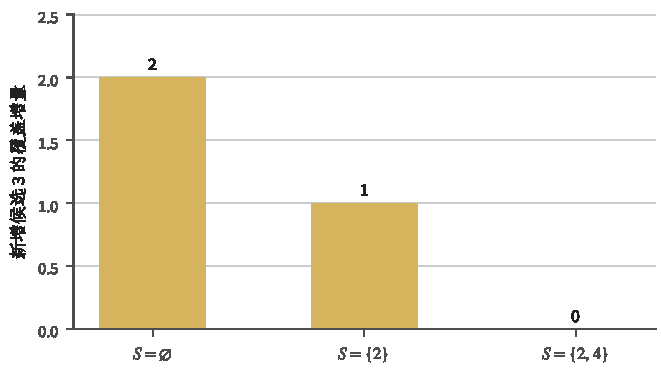
\includegraphics[width=\linewidth]{figures/math-preparation/probability-discrete/combinatorics-coverage-marginals.pdf}
  \caption{覆盖函数的有限教学构造。使用式~\eqref{eq:comb-running-coverage}中的\(Q_2,Q_3,Q_4\)，向\(\varnothing\subset\{2\}\subset\{2,4\}\)分别加入候选\(3\)，覆盖增量为\(2,1,0\)。柱高从零基线起画；图中只展示一个具体递减链，完整次模性仍由集合差证明。}
  \label{fig:combinatorics-coverage-marginals}
\end{figure}

\subsubsection{基数约束下的贪心保证}

次模性约束边际收益之间的关系，但只有与特定可行域和算法结合，才能得到求解保证
\scite{math-nemhauser1978submodular}
考虑归一化单调次模最大化
\[
  \max_{S\subseteq V,\ |S|\leq k}F(S),
  \qquad F(\varnothing)=0.
\]
贪心算法从$S^{(0)}=\varnothing$开始，在第$t$步选择边际收益最大的元素
\[
  e^{(t)}\in\argmax_{e\in V\setminus S^{(t)}}\Delta(e\mid S^{(t)}),
  \qquad
  S^{(t+1)}=S^{(t)}\cup\{e^{(t)}\}.
\]
平局可按固定顺序处理，使算法输出确定。

\begin{theorem}[单调次模最大化的贪心界]
\label{thm:comb-greedy-submodular}
设$1\leq k\leq|V|$，$F$归一化、单调且次模，$S^\star$是在
$|S|\leq k$下的最优解。
上述贪心算法运行$k$步得到$S^{(k)}$，则
\begin{equation}
  F(S^{(k)})
  \geq
  \left(1-\left(1-\frac1k\right)^k\right)F(S^\star)
  \geq(1-e^{-1})F(S^\star).
  \label{eq:comb-greedy-bound}
\end{equation}
\end{theorem}

\begin{proof}
固定第$t$步。由单调性、次模性以及逐个加入$S^\star\setminus S^{(t)}$中的元素，
\begin{align*}
  F(S^\star)-F(S^{(t)})
  &\leq F(S^{(t)}\cup S^\star)-F(S^{(t)})\\
  &\leq\sum_{e\in S^\star\setminus S^{(t)}}\Delta(e\mid S^{(t)}).
\end{align*}
右侧至多有$k$项，所以其中至少一项不小于
$[F(S^\star)-F(S^{(t)})]/k$。若右侧没有元素，则单调性已经给出
$F(S^{(t)})\geq F(S^\star)$，所需递推平凡成立；否则贪心选择的边际收益不小于上述某一项，
故
\[
  F(S^{(t+1)})-F(S^{(t)})
  \geq\frac{F(S^\star)-F(S^{(t)})}{k}.
\]
令剩余差距$r^{(t)}=F(S^\star)-F(S^{(t)})$，便有
$r^{(t+1)}\leq(1-1/k)r^{(t)}$。由$F(S^{(0)})=0$递推得到
\[
  r^{(k)}\leq\left(1-\frac1k\right)^kF(S^\star),
\]
移项给出第一个不等式。再用初等指数不等式$1-u\leq e^{-u}$（$0\leq u\leq1$），
得到$(1-1/k)^k\leq e^{-1}$，从而得到第二个不等式。
\end{proof}

定理~\ref{thm:comb-greedy-submodular}不能直接套到
式~\eqref{eq:comb-running-feasible-family}。逻辑规则形成的$\mathcal{C}_0$
不是普通基数约束，甚至不是向下封闭的：$\{1,3\}$可行，其子集$\{3\}$却不可行。
逐个加入当前边际收益最大的元素可能在中途违反规则，或走入无法扩展到最优解的分支。
其他约束下可以有不同的贪心、连续松弛或近似结果，但保证必须重新证明，不能只凭目标
具有次模性。

\subsection{扩大候选范围的最优值界}

把每个可行集合$S\in\mathcal C$写成指示向量$\bm z(S)\in\{0,1\}^n$，
得到整数可行点集$Z$。若用$P\subseteq[0,1]^n$放宽候选范围，就要求$Z\subseteq P$。
在$P$上选定目标$G$，并让$G(\bm z(S))=F(S)$对全部原候选成立，则
\[
  \max_{S\in\mathcal C}F(S)\leq\sup_{\bm z\in P}G(\bm z).
\]
原因只是原候选仍在扩大后的范围内；这里假设$\mathcal C$有限、非空且$F$实值。
任何取整后仍满足原规则的解则给出最大化目标的下界。对最小化问题，上下界方向相反。

例如考虑
\[
  \max\ z_1+z_2
  \quad\text{s.t.}\quad
  2z_1+2z_2\leq3,\qquad z_1,z_2\in\{0,1\}.
\]
整数最优值为$1$。放宽为$0\leq z_1,z_2\leq1$后，约束给出
$z_1+z_2\leq3/2$，而$(z_1,z_2)=(1,1/2)$恰好达到$3/2$，所以它是松弛最优值，
确实是整数最优值的上界。
若把正坐标都取为$1$，则得到$(1,1)$并违反容量约束；若把$1/2$向下取整，则恢复一个
值为$1$的可行解。这个算例同时展示了松弛界、取整可行性与取整后目标值是三项不同检查。

本小节只利用候选范围的包含关系建立界。松弛集合的几何结构如何影响最优值，
以及取整后的可行性与目标误差怎样判断，将在后续第~\ref{sec:opt-relaxations-certificates}节
展开；目标具有次模性本身还不足以回答这些问题。

\section{问题族的可计算性与复杂度}
\label{sec:comb-computability-complexity}

前节规定了什么结果算作合法答案，并给出了特定选择算法的质量保证。
现在把考察对象换成整类输入及处理它们的统一程序：程序是否对规定输入正确终止，以及
时间、空间和证书规模怎样随输入增长，是两类独立要求。
通用可计算性并不从属于候选计数；即使每个实例都由有限字符串编码，关于程序行为的
整个问题族仍可能不可判定。有限候选可枚举与枚举成本可承受也须分开。

\subsection{输入编码与计算模型}

复杂度不是对象本身附带的标签，而是相对于输入编码、计算模型和所求输出定义的。
对有限变量问题，可以把$n$、CNF公式、整数或有理数权重以及阈值写成有限比特串。
输入长度记为$L$，它包括变量索引、子句、数值的二进制位数和分隔信息。
若一个权重需要$b$位表示，读取和比较它就不能无条件算作与$b$无关的一步。

同一优化任务常对应三个不同计算问题。
\begin{itemize}
  \item \term{搜索问题}要求返回一个满足$\Phi$的$\bm{z}$；
  \item \term{优化问题}要求返回目标最优的可行$\bm{z}$或最优值；
  \item \term{判定问题}只问是否存在满足$\Phi$且$F(S(\bm{z}))\geq K$的赋值。
\end{itemize}
复杂性类别通常先为判定问题定义。若能多次调用判定算法并固定变量，常可恢复一个解；
但调用次数、数值精度和自归约结构都要计入，不能把“知道答案存在”直接当作已经构造答案。

\subsection{可枚举、可判定与可计算}

按顺序输出候选、回答某个输入是否属于集合，以及计算一个函数值，要求程序提供不同的
信息。特别是等待某个候选出现时，暂时没有看到它，并不能给出“永远不会出现”的答案。
下面都以有限字符串作为输入编码，以一个固定、有限描述的程序处理全部允许输入。
\begin{definition}[可枚举、可判定与可计算]
\label{def:comb-computability}
一个对象集合若存在程序依次输出其中全部对象，称为\term{可枚举的}
（computably enumerable）。这里要求程序只输出该集合中的对象，并最终输出其中每个
对象；程序可以重复输出，也不必告诉我们某个尚未出现的对象
以后是否会出现。一个判定问题若存在程序对每个合法输入都在有限步内停机，并正确回答
“是”或“否”，称为\term{可判定的}（decidable）。若程序只保证在“是”实例上最终
停机并接受，而在“否”实例上可能永不停止，则称该问题\term{半可判定的}
（semidecidable）。
类似地，定义在全部有限字符串上的函数$f$若存在一个程序，对每个输入$x$都停机并输出
$f(x)$，就称$f$为\term{可计算函数}（computable function）。若讨论部分函数，
还要求程序恰在其定义域内停机并输出相应值，域外输入不停止；仅承诺处理一个指定子集
属于另一种带输入承诺的问题约定。
\end{definition}
判定问题可看作计算
取值为$0$或$1$的特征函数，因此可判定性比只确认正例的半可判定性要求更强。

可枚举不等于可判定。若某集合及其补集都可枚举，可以交错运行两个枚举或半判定程序：
输入最终会被其中一方确认，于是得到判定程序。若只有正例可枚举，等待尚未出现的对象
无法证明它永远不会出现。

在明确的有限编码下，CNF可满足性是可判定的。按字典序枚举全部
$2^n$个赋值，每个赋值逐子句检查；找到满足赋值就回答“是”，全部检查完仍未找到则
回答“否”。若公式有$m$个子句、总文字出现次数为$q$，直接实现需要
$O(2^n q)$量级的时间和存放当前赋值及公式所需的空间。这个算法很慢，但一定停机，
所以它证明了可判定性。

“每个实例的候选集有限”还不足以独立构成上述证明。程序必须能从输入有效得到候选编码，
能判定一个候选是否满足约束，并能知道枚举何时完成。若把一个不可计算实数或一个可能
不停机的黑盒藏进“目标求值”，有限个候选也未必能被统一程序比较。可计算性要求的是
对整族输入存在同一个有限描述的程序。

\subsection{不可判定性与停机问题}

有限变量问题在有效表示下可以穷举，但一般程序的行为并非总能判定。
令
\[
  \mathrm{HALT}
  =
  \{(P,x):\text{程序 }P\text{ 在输入 }x\text{ 上最终停机}\}.
\]
它是半可判定的：模拟$P(x)$，若模拟停止就接受；若$P(x)$永不停止，模拟也不会给出
否定答案。下面的对角论证说明不存在总能判断停机与否的程序。

停机问题的不可判定性是可计算性理论的基本结论\scite{math-turing1937computable}
\begin{theorem}[停机问题不可判定]
\label{thm:comb-halting-undecidable}
$\mathrm{HALT}$不可判定。
\end{theorem}

\begin{proof}
反设存在判定程序$H(P,x)$，它总会停机，并在$P(x)$停机时返回$1$，否则返回$0$。
据此构造程序$D$：输入一个程序编码$P$，先计算$H(P,P)$；若结果为$1$，就进入无限
循环；若结果为$0$，就立即停机。

现在把$D$自己的编码交给$D$。若$H(D,D)=1$，按照$D$的定义，$D(D)$进入无限循环，
与$H$判断它会停机矛盾。若$H(D,D)=0$，$D(D)$立即停机，又与$H$判断它不停机矛盾。
两种返回值都导致矛盾，所以这样的判定程序$H$不存在。
\end{proof}

定理~\ref{thm:comb-halting-undecidable}区分了“某次模拟尚未结束”和“已经证明不会结束”。
前者是有限时刻的观察，后者要求排除所有未来时刻。不可判定也不等于每个具体程序都无法
分析；许多程序可由终止度量、循环不变量或有限状态搜索证明停机。结论是不存在一个对
任意程序和输入都正确的统一判定器。

\subsection{多项式时间、证书与复杂性类别}

可判定问题仍可能需要随输入长度急剧增长的资源。能统一快速求解，与只能快速核对给定答案，
是不同的计算要求。
\begin{definition}[复杂性类别P与NP]
\label{def:comb-p-np}
若存在一个对所有实例都正确判定的确定性算法，其最坏运行时间由
$L$的某个固定次数多项式控制，该判定问题属于复杂性类别$\mathrm{P}$。
类别$\mathrm{NP}$包含满足如下条件的判定问题$\mathcal{L}$：存在多项式$p$和确定性
多项式时间验证程序$\mathsf{Ver}$，使每个输入$x$都满足
\[
  x\in\mathcal{L}
  \quad\Longleftrightarrow\quad
  \exists y,\quad |y|\leq p(|x|),\quad \mathsf{Ver}(x,y)=1.
\]
其中$|x|$是输入的比特长度，$y$称为\term{证书}（certificate）。
\end{definition}
双向条件不仅要求
每个“是”实例存在可接受的多项式长度证书，还要求“否”实例的所有这类证书都被拒绝。
名称中的“非确定性”描述这种猜测证书后验证的计算模型，不表示算法可以容忍随机错误。
确定性多项式算法的运行轨迹本身可作证书，所以
$\mathrm{P}\subseteq\mathrm{NP}$。目前并不知道这个包含是否严格；把
$\mathrm{P}\neq\mathrm{NP}$当作已经证明的事实，会超出这里可用的结论。

CNF可满足性属于$\mathrm{NP}$。证书就是$n$位赋值$\bm{z}$，验证程序逐个检查子句，
时间关于公式长度为线性量级。穷举证明它可判定，短证书证明它属于$\mathrm{NP}$；
二者都没有给出多项式时间的求解算法。

\begin{definition}[多项式时间多对一归约]
\label{def:comb-polynomial-reduction}
若判定问题$A$的每个实例$x$都能在多项式时间内变换为判定问题$B$的实例$f(x)$，并满足
\[
  x\in A\quad\Longleftrightarrow\quad f(x)\in B,
\]
就称$A$可\term{多项式时间多对一归约}（polynomial-time many-one reduction）
到$B$，记作$A\leq_{\mathrm{p}}B$。
\end{definition}
归约方向表示：若能高效解决$B$，就能先计算
$f(x)$再高效解决$A$。因此从已知困难问题归约到新问题，才能证明新问题至少同样困难；
把方向写反不会得到这个结论。

\begin{definition}[NP困难与NP完全]
\label{def:comb-np-hard-complete}
一个判定问题若所有$\mathrm{NP}$问题都可多项式时间归约到它，就称为
\term{NP困难}（NP-hard）；若它还属于$\mathrm{NP}$，就称为
\term{NP完全}（NP-complete）。
\end{definition}
Cook--Levin定理给出SAT是NP完全问题
\scite{math-cook1971complexity}通过引入
辅助变量，可以把一般公式在多项式时间内变成等可满足的CNF公式；再把长子句拆成由辅助
变量连接的三文字子句，可以归约到3-SAT。这里的“等可满足”只保证原公式有解当且仅当
新公式有解，不要求辅助变量加入后两个公式拥有相同的模型集合。由这些接口可知CNF-SAT
与3-SAT也都是NP完全问题。这里把结论作为复杂度理论的基准，不展开对任意多项式时间
验证计算的编码证明；下面只证明与本章约束表示直接相关的归约。

\begin{theorem}[CNF可满足性归约到零一线性可行性]
\label{thm:comb-sat-to-binary-linear}
给定任意CNF公式，可以在关于公式长度的多项式时间内构造一组零一线性不等式，
使该公式可满足当且仅当这些不等式存在零一可行解。因此零一线性可行性是NP困难的；
当所有整数系数按二进制编码时，它也属于NP，因而是NP完全的。
\end{theorem}

\begin{proof}
为每个命题变量建立$z_i\in\{0,1\}$。对每个子句
$C=\ell_1\lor\cdots\lor\ell_r$，加入式~\eqref{eq:comb-clause-linearization}：
\[
  \sum_{j=1}^{r}v(\ell_j)\geq1.
\]
每个文字只产生一个系数为$1$的变量项或$1-z_i$，所以构造时间和输出长度都关于原公式
长度为线性量级。

若原公式有满足赋值，把真假分别编码为$1,0$。每个子句至少一个文字为真，对应不等式
左侧至少为$1$，所以得到零一可行解。反过来，任一零一可行解定义一个布尔赋值；
每条不等式左侧至少为$1$，说明相应子句至少一个文字为真，故全部子句同时满足。
两边可行性等价，归约成立。

由CNF可满足性的NP困难性，零一线性可行性NP困难。对其NP成员关系，证书是一组零一
变量值；验证者按二进制整数运算检查所有不等式，所需时间关于输入和证书长度为多项式。
\end{proof}

定理~\ref{thm:comb-sat-to-binary-linear}说明，换成代数记号不会自动消除逻辑搜索的
困难。它也没有声称每个零一线性实例都难：式~\eqref{eq:comb-running-integer-constraints}
只有四个变量，可以立即求解；某些约束矩阵或关系结构还允许专门的多项式算法。
NP完全描述的是一族问题在最坏情况下的归约地位，不是每个实例的运行时间预测。

\subsection{复杂度结论的边界}

输入规模必须与算法成本使用同一口径。枚举$2^n$个赋值是关于变量数$n$的指数时间；
若输入本身已经显式列出全部$2^n$个候选，那么扫描列表反而关于输入长度是线性的。
把隐式表示与显式列表混在一起，会让同一算法同时被误称为指数和线性。

数值大小也不能替代编码长度。若整数$N$用二进制给出，输入它只需
$\lfloor\log_2N\rfloor+1$位；执行$N$轮的循环关于数值$N$是线性的，却关于输入位数
是指数级的。运行时间关于数值大小是多项式、关于二进制输入长度却未必是多项式的算法，
称为\term{伪多项式时间算法}（pseudo-polynomial-time algorithm）。只有同时说明
数值编码与所计基本运算，才能判断一个界是否真正关于输入长度为多项式。

最坏情况复杂度也不同于一次实验运行时间。某个求解器在当前数据上很快，可能来自实例
结构、预处理或启发式分支顺序；这不能证明问题属于$\mathrm{P}$。反过来，NP完全性
不排除小实例、特殊结构、参数受限情形或近似目标能够高效求解。应说明保证针对精确解、
近似值还是可行解，并列明依赖的参数与表示。

统计样本量与计算时间同样不能互相替代。一个候选族可能只需较少样本就能控制泛化误差，
经验风险最小化却仍难以计算；也可能存在高效优化算法，但样本不足以区分多个预测规则。
可计算学习还要求训练程序和输出的预测程序都停机，高效学习进一步要求相应资源由规定
参数的多项式控制。组合计数可以进入统计界，也可以进入枚举成本，但两处的规模对象和
结论必须分别核对。

\subsection{数学答案与程序保证的区别}

程序保证需要与数学答案的性质分开。回看式~\eqref{eq:prelim-regularized-least-squares}，
“求一个最小值”至少涉及下面四种不同要求，计算资源还在可计算性之外另加限制。

\begin{table}[htbp]
  \centering
  \small
  \begin{tabularx}{\linewidth}{@{}lX@{}}
    \toprule
    \textbf{问题} & \textbf{需要回答的内容} \\
    \midrule
    存在性 & 是否有$\bm{w}^\star$真正达到$\inf_{\bm{w}}F(\bm{w})$。 \\
    唯一性 & 达到最优值的参数是否只有一个。 \\
    可识别性 & 不同参数是否会产生相同的可观测预测或数据分布。 \\
    可计算性 & 是否有对规定输入终止并给出正确结果的统一程序；精度和资源界需另行说明。 \\
    \bottomrule
  \end{tabularx}
  \caption{最优化陈述中的四类不同要求。每一行需要不同的条件与论证。}
  \label{tab:prelim-four-solution-questions}
\end{table}

这四类问题彼此相关，却不能相互替代。一个有限非空候选集上的实值函数必定达到最小值，
但若没有给出枚举候选或计算函数值的有效方式，存在性本身不提供实际算法。例
\ref{ex:prelim-nonidentifiable-parameterization}中的参数不可唯一识别，但乘积$ab$
对应的预测函数仍可唯一确定。反过来，即使目标函数只有一个最小点，有限精度计算通常也
只能返回近似值；能否精确到达该点，或能在多大误差内逼近它，需要单独的算法保证。

回到带正则项的最小二乘。它的变量属于$\mathbb{R}^d$，目标值属于$\mathbb{R}$，
样本索引$i$遍历同一组$n$个观测，$\lambda$控制第二项的权重。若要声称某算法返回唯一
的目标最优点，需要分别证明最小点存在、最小点唯一，以及算法确实到达该点；若算法只给出
误差保证，则应改称它在规定成本下得到近似解。只有进一步声称该参数可由观测唯一确定，
或算法恢复了真实参数时，才需要额外证明数据与参数化具有所需的可识别性。后续章节将在
各自需要时分别给出这些条件。

\section{本章小结}
\label{sec:comb-summary}

候选空间、求解任务和程序是三个不同的考察对象。精确计数与增长尺度说明结果数量怎样
变化，容斥校正重叠，Möbius反演恢复累计量中的局部贡献。函数族的限制类记录有限输入上
可实现的标记；VC维及多类别维度约束模式丰富度，实值函数还要固定阈值与间隔。
这些容量结论不直接给出训练或求解算法的运行时间。

规则与目标共同规定答案。检查一个赋值、判定有解、构造见证与取得最优结果不能混用；
子句的零一转换保持逻辑可行性，连续松弛和软代价则改变允许对象或比较准则。
覆盖的边际递减配合单调性与基数约束，才能给出贪心质量界；松弛界还需另外检查取整后的
可行性和目标误差。存在一个最佳候选，并不自动给出找到它的程序。

统一程序必须处理规定的整类输入。可枚举、可判定与可计算分别说明程序能提供什么回答，
停机问题展示一般程序任务的不可判定边界；多项式时间、证书与归约则讨论资源和困难度。
结果数量、答案质量、终止保证、计算成本与统计样本量各有自己的对象和条件。
当候选连续变化或迭代无限延续时，还需第~\ref{chap:mathematical-analysis}章的
测度、极限与连续性工具；第~\ref{chap:graph-theory}章会进一步研究关系结构怎样改变
路径、分离和计算组织。

\chapter{测度与分析}
\label{chap:mathematical-analysis}

第~\ref{chap:sets-functions-and-proofs}章建立对象与条件的语言，第~\ref{chap:combinatorics}章
研究有限选择与计算。本章转向它们留下的无限过程：部分和不断延长，递推持续更新，
一个函数在连续区域上累计，或者一列近似函数逐渐提高精度。有限步骤中的规则能否
保留到极限，取决于比较对象的结构、采用的误差尺度及可核对的控制条件。

本章面向已经学过基础分析、线性代数、概率与组合数学的理工科本科毕业生。
熟悉的极限、求导与积分按用途回顾，把主要解释放在一般空间、测度与极限交换上。
集合的距离与权重是共同基础：距离说明点如何接近，测度说明范围占多少贡献。
序列据此讨论极限、累计与迭代保证；固定一个函数时，局部变化和整体累计承担不同任务。
当函数本身随索引变化，还要判断连续性、导数和积分究竟能否保留。
这条路线把集合、点列、单函数和函数列连起来，也使“有极限”与“可以交换运算”分开。

\section{集合的距离、权重与可测范围}
\label{sec:analysis-set-structures}

第~\ref{chap:sets-functions-and-proofs}章已经给出集合、映射和等价关系。现在同一个集合
还可以承担两项不同的任务：判断两个点是否接近，以及累计一个范围内的贡献。
前一任务需要距离，后一任务需要为集合分配权重。距离确定邻域，可测集合族确定哪些
范围允许赋权；两者可以相容，却不能互相代替。

\subsection{度量与邻域}

实数可以用绝对值之差比较，但一个状态也可能是向量、一张函数或一组概率权重。
此时先要指定什么差异算大、什么差异算小。度量把这种比较归纳为三条规则：
零距离应能辨认同一个对象，比较不分先后，绕经第三个点不会比直接比较更短。
\begin{definition}[度量与度量空间]
\label{def:analysis-metric-space}
集合$X$上的\term{度量}（metric）是函数$d:X\times X\to[0,\infty)$，满足对任意$x,y,z\in X$，
\[
  \begin{aligned}
    d(x,y)=0&\Longleftrightarrow x=y,\\
    d(x,y)&=d(y,x),\\
    d(x,z)&\leq d(x,y)+d(y,z).
  \end{aligned}
\]
带有度量的集合$(X,d)$称为\term{度量空间}（metric space）。
\end{definition}
欧氏空间使用$d(\bm{x},\bm{y})=\lVert\bm{x}-\bm{y}\rVert_2$；有限集合可以使用离散度量$d(x,y)=\mathbb{I}\{x\neq y\}$。同一个集合选择不同度量，可能改变何谓收敛以及函数是否连续；不过，有些度量只改变数值尺度，例如$d$与$2d$具有相同的收敛序列和连续映射。不能仅凭距离公式不同就断言这些性质不同。

\begin{definition}[开球]
\label{def:analysis-open-ball}
在度量空间$(X,d)$中，以$x\in X$为中心、半径$r>0$的开球记为
$B(x,r)=\{y\in X:d(x,y)<r\}$。
\end{definition}

开球把“离一个点足够近”写成集合。若$V\subseteq X$包含某个$B(x,r)$，就称
$V$是$x$的邻域；邻域本身不必是开集。由这些邻域还可以判断一个范围是否包含
其中每个点附近的点。

\begin{definition}[开集与闭集]
\label{def:analysis-open-closed-sets}
在度量空间$(X,d)$中，集合$U\subseteq X$若对每个$x\in U$都存在$r>0$使$B(x,r)\subseteq U$，就称为
\term{开集}（open set）；集合$C\subseteq X$若其补集$X\setminus C$为开集，就称为
\term{闭集}（closed set）。
\end{definition}

开闭性总是相对于当前空间而言。例如$[0,1/2)$在$\mathbb R$中不是开集，
但在子空间$X=[0,1]$中是开集：此时开球是实轴开区间与$X$的交，
$0$的一个小球不必包含负数。全集$X$和空集既开又闭；“不是开集”也不等于
“就是闭集”，实轴上的$[0,1)$便两者都不是。

同一集合上的距离选择也应随比较任务变化。在$\mathbb R$上，通常距离
$d_1(x,y)=|x-y|$把数值相近的状态看作接近，离散距离
$d_2(x,y)=\mathbb I\{x\neq y\}$则只区分相同与不同。
点$0$的$d_1$小球是区间，而半径小于$1$的$d_2$球只有$\{0\}$。
在有限状态的概率向量$\bm p,\bm q$之间，$\sum_i|p_i-q_i|$比较的是整组
权重的差异；在有界函数$f,g:S\to\mathbb R$之间，
$\sup_{x\in S}|f(x)-g(x)|$比较的是所有输入处的最大误差。
后两种距离的点分别是概率向量和函数，不能用一个未指定坐标的实数绝对值代替。
后文会用$1/n$和恒等映射具体核对$d_1,d_2$对收敛、连续性的不同判断。

有时比较规则只能看到对象的一部分，因而会把两个不同对象判为零距离。例如在
$\mathbb R^2$中只比较第一个坐标，$d(\bm x,\bm y)=|x_1-y_1|$仍保留对称性和
三角不等式，却无法区分$(0,0)$与$(0,1)$。后面的样本函数距离和半正定二次型
都需要表达这种分辨力有限的比较。
\begin{definition}[伪距离]
\label{def:analysis-pseudometric}
集合$X$上的\term{伪距离}（pseudometric，也称伪度量）是函数
$d:X\times X\to[0,\infty)$，对所有$x,y,z\in X$满足
\[
 d(x,x)=0,\qquad d(x,y)=d(y,x),\qquad d(x,z)\leq d(x,y)+d(y,z).
\]
它允许$x\neq y$时仍有$d(x,y)=0$；若进一步要求零距离蕴含$x=y$，就得到度量。
\end{definition}
零距离并不意味着原始对象相等。若任务本来就不区分这些对象，可以把它们合并：
定义$x\sim y$当且仅当$d(x,y)=0$。自反性、对称性及三角不等式分别保证这是一项
等价关系。在商集$X/{\sim}=\{[x]:x\in X\}$上定义
\begin{equation}
 \bar d([x],[y])=d(x,y).
\label{eq:analysis-quotient-metric}
\end{equation}
这一定义必须不依赖代表元。若$x\sim x'$且$y\sim y'$，则
$d(x,y)\leq d(x,x')+d(x',y')+d(y',y)=d(x',y')$；交换两对点又得反向不等式，
故距离相等。其余度量条件直接继承，而且$\bar d([x],[y])=0$恰好等价于
$[x]=[y]$，所以商集确实成为度量空间。

在只看第一坐标的例子中，$[(a,b)]=\{(a,t):t\in\mathbb R\}$是一条竖直直线；
商空间中的点是这些直线，两点距离为第一坐标之差的绝对值。原空间丢失的第二坐标
没有被恢复，而是被明确排除在比较对象之外。
第~\ref{sec:analysis-function-convergence-essential-bounds}节中的函数等价类会回用这一做法。

\subsection{测度与可测集}
\subsubsection{可测集合与赋权}

前文的\emph{度量}$d(x,y)$比较两个点相距多远，此处的\emph{测度}$\mu(A)$描述
整个集合$A$占多少权重。两者处理不同对象，并不存在从距离公式直接得到唯一测度的
通用规则。例如$X=\{a,b\}$可以固定离散度量$d(a,b)=1$，却分别使用计数权重
$(1,1)$、非均匀权重$(1,2)$，或归一化后的概率权重$(1/3,2/3)$。
点列的收敛不因此改变，函数的积分却随权重改变。
表~\ref{tab:analysis-metric-measure-integral}把这几个对象分开。

\begin{table}[htbp]
 \centering\small
 \begin{tabularx}{\linewidth}{@{}lXX@{}}
 \toprule
 对象 & 比较或汇总什么 & $X=\{a,b\}$上的例子\\
 \midrule
 度量$d$ & 两点的距离 & $d(a,b)=1$\\
 测度$\mu$ & 集合的权重 & $\mu(\{a\})=1$，$\mu(\{b\})=2$\\
 积分$\int f\,\mathrm d\mu$ & 函数值的加权总量 & $f(a)+2f(b)$\\
 平均 & 总量除以总权重 & $[f(a)+2f(b)]/3$\\
 \bottomrule
 \end{tabularx}
 \caption{距离与权重的不同职责。固定同一个距离仍可选择不同测度；只有总权重为$1$时，积分本身才直接是平均。}
 \label{tab:analysis-metric-measure-integral}
\end{table}

在连续空间中，不能只给每个点一个长度再逐点相加：单点的长度为零，区间的长度却可以
为正。需要直接给适当的\emph{集合}赋值，并要求把集合分割后，所有不重叠部分的大小
能够相加。为此还要说清哪些集合允许参与这一运算。下面的集合族列出允许测量的范围，
并保证取补集、合并可数多个范围后，结果仍在这个范围内。

\begin{definition}[$\sigma$代数与可测空间]
\label{def:analysis-sigma-algebra}
设$X$为集合。若子集族$\mathcal{A}\subseteq\mathcal{P}(X)$满足
\[
  \begin{gathered}
    X\in\mathcal{A},\\
    A\in\mathcal{A}\Longrightarrow X\setminus A\in\mathcal{A},\\
    A_1,A_2,\ldots\in\mathcal{A}
    \Longrightarrow\bigcup_{n=1}^{\infty}A_n\in\mathcal{A}.
  \end{gathered}
\]
则称$\mathcal{A}$为$X$上的\term{$\sigma$代数}（sigma-algebra）。二元组
$(X,\mathcal{A})$称为\term{可测空间}（measurable space），$\mathcal{A}$中的集合称为
相对于$\mathcal{A}$的\term{可测集合}（measurable set）。
\end{definition}
这些条件还蕴含$\varnothing\in\mathcal{A}$及对可数交封闭。只要求可数次运算而非任意次
运算，是因为极限与可数序列相连，同时又能避免给所有过于复杂的子集强行赋予相容的长度。

选定可以测量的集合后，还需给它们分配相容的权重。相容的关键是：可数个互不重叠
部分的总权重，应等于各部分权重之和。
\begin{definition}[测度与测度空间]
\label{def:analysis-measure-space}
设$(X,\mathcal{A})$为可测空间。映射$\mu:\mathcal{A}\to[0,\infty]$若满足
$\mu(\varnothing)=0$，并且对任意两两不交的$A_1,A_2,\ldots\in\mathcal{A}$有
\[   \mu\left(\bigcup_{n=1}^{\infty}A_n\right)   =   \sum_{n=1}^{\infty}\mu(A_n). \]
则称$\mu$为\term{测度}（measure）。上述等式称为可数可加性，三元组
$(X,\mathcal{A},\mu)$称为\term{测度空间}（measure space）。
\end{definition}
定义中的非负无穷和约定为有限部分和的上确界：
\[
  \sum_{n\geq1}a_n=\sup_{N\geq1}\sum_{n=1}^N a_n,\qquad a_n\geq0.
\]
结果允许为$+\infty$。这只回用第~\ref{chap:sets-functions-and-proofs}章的有限和与上确界；第~\ref{sec:analysis-sequences-series-errors}节再研究一般级数的收敛。

实数上的Lebesgue测度把区间$(a,b)$赋值为$b-a$；有限集合上的计数测度把集合赋值为
元素个数；给有限点$x_i$分配质量$w_i\geq0$则得到$\mu(A)=\sum_{i:x_i\in A}w_i$。
因此有限加权和、通常的面积积分和后续的概率期望可以使用同一套记号
\scite{math-folland1999real}

测度还保留集合包含的大小关系。若可测集合$A\subseteq B$，把$B$分成不交的
$A$与$B\setminus A$，便有$\mu(B)=\mu(A)+\mu(B\setminus A)\geq\mu(A)$。
这项单调性将在零测集和集合极限中使用，不需要先定义函数积分。


度量与测度的常见联系发生在“哪些集合可测”这一层。度量先确定开集；把开集及其
可数集合运算得到的集合纳入测量范围，就得到下面的标准选择。
\begin{definition}[Borel $\sigma$代数]
\label{def:analysis-borel-sigma-algebra}
在度量空间$(X,d)$中，包含所有开集的最小$\sigma$代数记为$\mathcal{B}(X)$，称为
\term{Borel $\sigma$代数}（Borel sigma-algebra）；其中的集合称为Borel集合。
\end{definition}
“最小”指它包含在每个含有所有开集的$\sigma$代数中。实数上的开区间、闭区间和
单点因而都是Borel集合。度量由此提供一族可测集合，却还没有指定它们的权重；在实数上，
长度测度与把全部权重集中在某一点的测度，都可以定义在同一族Borel集合上。

\subsubsection{集合极限与测度连续性}
\label{sec:analysis-set-measure-continuity}
可测范围逐步扩大时，已经纳入的权重会不会在极限中丢失？记
$A_n\uparrow A$表示$A_n\subseteq A_{n+1}$且$A=\bigcup_nA_n$；
记$A_n\downarrow A$表示$A_n\supseteq A_{n+1}$且$A=\bigcap_nA_n$。
这两种集合极限分别保留所有最终进入的点、所有始终没有被排除的点。
可数可加性给出相应的测度连续性。以下各集合均属于可测集合族$\mathcal A$。若
$A_1\subseteq A_2\subseteq\cdots$且$A=\bigcup_nA_n$，令
$B_1=A_1$、$B_n=A_n\setminus A_{n-1}$，则$B_n$两两不交且
$A_n=\bigcup_{k=1}^nB_k$。因此
\[
  \mu(A)
  =
  \sum_{k=1}^{\infty}\mu(B_k)
  =
  \lim_{n\to\infty}\mu(A_n).
\]
这里的极限就是非负有限部分和的上确界，允许为无穷，不依赖函数积分。
例如实轴上的$A_n=(0,1-1/n)$递增到$(0,1)$，其长度$1-1/n$也趋于$1$；
端点$1$虽然从未进入集合，但集合的极限仍有完整的单位长度。

若$A_1\supseteq A_2\supseteq\cdots$且$\mu(A_1)<\infty$，令$A=\bigcap_nA_n$。
对递增集合$A_1\setminus A_n$应用上一结论，得到
\[
 \mu(A_1)-\mu(A)
 =\mu(A_1\setminus A)
 =\lim_n\mu(A_1\setminus A_n)
 =\mu(A_1)-\lim_n\mu(A_n).
\]
所有相减项均有限，故$\mu(A)=\lim_n\mu(A_n)$。
例如$[0,1/n]\downarrow\{0\}$且长度趋于$0$。
递减情形需要$\mu(A_1)<\infty$：
若每个$A_n$的测度都为无穷，就不能通过“无穷减无穷”得到结论。例如Lebesgue测度下
$A_n=(n,\infty)$递减到空集，但每个$A_n$的测度仍为无穷。

\subsubsection{零测例外与测度完备性}
这种权重允许某些非空集合的大小为零。讨论积分和函数极限时，这些集合上的例外
往往不影响总量；“几乎处处”就是把这种可忽略性说清楚。
\begin{definition}[零测集与几乎处处]
\label{def:analysis-null-set-almost-everywhere}
在测度空间$(X,\mathcal{A},\mu)$中，若$N\in\mathcal{A}$且$\mu(N)=0$，称$N$为
\term{零测集}（null set）。若存在这样的$N$，使某性质对每个$x\in X\setminus N$
成立，称该性质$\mu$-\term{几乎处处}（almost everywhere，简写为a.e.）成立。
\end{definition}
这里不要求例外集合为空，而是要求它包含在一个可测的零测集中。换用另一个测度后，
原来的例外可能不再可忽略。例如单点在长度测度下为零，在计数测度下却有质量$1$。

还会遇到另一项要求：一个集合既然没有权重，它的任何子集也应能被赋予零权重。
这项要求并非由可数可加性自动保证，因此需要单独说明。
\begin{definition}[完备测度空间]
\label{def:analysis-complete-measure-space}
若测度空间$(X,\mathcal{A},\mu)$中每个零测集$N$的任意子集$E\subseteq N$都属于
$\mathcal{A}$，称该测度空间完备。此时由测度的单调性还有$\mu(E)=0$。
\end{definition}
把可测零测集的所有子集加入原$\sigma$代数，并相应扩展测度，称为测度空间的完备化。
具体地，令
\[
 \begin{aligned}
 \overline{\mathcal A}
 &=\left\{A\cup E:
     \begin{array}{l}
       A,N\in\mathcal A,\quad \mu(N)=0,\\
       E\subseteq N
     \end{array}\right\},\\
 \bar\mu(A\cup E)&=\mu(A).
 \end{aligned}
\]
若同一集合还有表示$A'\cup E'$，则$A\setminus A'$和$A'\setminus A$
都包含在一个可测零测集中；这两个差集本身可测，故测度为零，
由有限可加性得$\mu(A)=\mu(A')$，赋值不依赖表示。
取补集时，可把$A\cup E$的补集写成
$(X\setminus(A\cup N))\cup(N\setminus(A\cup E))$；
第二项仍是零测集的子集。取可数并时，可测部分取并，例外部分包含在零测集的可数并中，
因而$\overline{\mathcal A}$是$\sigma$代数。对两两不交的$A_j\cup E_j$，
其可测部分$A_j$也两两不交，$\bar\mu$的可数可加性随即由$\mu$继承。
若$\bar\mu(A\cup E)=0$，则$A\cup E$包含在原可测零测集$A\cup N$中；
它的任意子集已被纳入$\overline{\mathcal A}$，所以扩展后的空间完备。

一个有限例子能看清增加了什么。取$X=\{a,b,c\}$、
$\mathcal A=\{\varnothing,\{a,b\},\{c\},X\}$，令$\mu(\{a,b\})=0$、
$\mu(\{c\})=1$。原来不能单独测量$\{a\}$；完备化把$\{a\}$、$\{b\}$
及其与$\{c\}$的并纳入，得到全部子集，并把新增零测子集赋值为零。
实数上的Lebesgue测度空间则是Borel长度测度空间的完备化；新增的集合仍保持相容的长度。
这里的完备性处理零测集的子集，不同于第~\ref{sec:analysis-sequences-series-errors}节中
“柯西数列不会逃出空间”的完备性。

\section{序列的极限、累计与迭代收敛}
\label{sec:analysis-sequences-series-errors}

索引族说明怎样排列对象，尚未说明项数增加以后会发生什么。这里从熟悉的实数列
出发，再把收敛和柯西条件推广到向量及一般度量空间中的点列；每一项不必是一个数。
部分和与递推更新都产生这样的序列，因而可以用同一套极限工具判断累计是否稳定、
更新是否得到解，以及有限步计算距离最终结果还有多远。

\subsection{序列极限与空间完备性}
\subsubsection{数值极限与上下极限}

\term{数列}（sequence）是以自然数为索引的一族数，写作$(a_n)_{n\geq 1}$。若对每个$\varepsilon>0$，都存在只依赖于$\varepsilon$的整数$N$，使得
\[   n\geq N\quad\Longrightarrow\quad |a_n-a|<\varepsilon, \]
就称$a_n$\term{收敛}（converge）到$a$，记作$a_n\to a$。这一定义要求同一个 $N$控制其后的全部项，而不是只要求数列偶尔靠近$a$。极限若存在便唯一：若$a\neq b$ 都是极限，取$\varepsilon=|a-b|/3$，充分靠后的$a_n$会同时落入两个不相交的邻域， 产生矛盾。

收敛数列必有界。事实上，取$\varepsilon=1$后，除有限个前项外都有 $|a_n|\leq |a|+1$，再把有限个前项的绝对值一并取最大值即可。反向结论通常不成立， 例如$a_n=(-1)^n$有界却不收敛。若再加入单调性，情况便不同。

这里需要使用实数的\term{完备性}（completeness）。它的一种等价表述是确界公理：
每个非空且有上界的实数集合都有实数上确界。稍后讨论柯西数列时，还会看到完备性的
另一种等价表述。
\begin{theorem}[单调有界收敛定理]
\label{thm:analysis-monotone-bounded-sequence}
若实数列$(a_n)$单调不减且有上界，则$a_n$收敛到 $a=\sup\{a_n:n\in\mathbb{N}\}$。单调不增且有下界的情形类似。
\end{theorem}
这里回顾该结论，不再展开熟悉的证明。“有界”与“单调”缺一不可：$n$单调却无上界，$(-1)^n$有界却不单调。这一结论还依赖实数的完备性；若只在有理数中考察逐步逼近$\sqrt{2}$的有理数列，所有项都在有理数中，极限却不在这个空间中。下一项将把这种“柯西数列的极限仍留在空间内”的性质推广到一般度量空间。

无有限极限的数列称为发散，但发散不一定意味着振幅越来越大。$(-1)^n$始终振荡，
而$a_n=n$趋于正无穷。准确地说，
\[
 a_n\to+\infty
 \quad\Longleftrightarrow\quad
 \forall M\in\mathbb R,\ \exists N,\ \forall n\geq N,\ a_n>M;
\]
趋于负无穷把最后的不等式改为$a_n<M$。这不是仅要求某些项很大。
$\overline{\mathbb R}=\mathbb R\cup\{-\infty,+\infty\}$称为扩展实数，
用于记录这类边界结果；$\infty-\infty$仍没有定义。

后文还会按条件使用几个熟悉结论：若$a_n\to a$、$b_n\to b$且$a,b$有限，
和、积的极限分别是$a+b$、$ab$；商的规则还要求$b\neq0$。
若充分大的$n$满足$a_n\leq c_n\leq b_n$，且两端同趋于$c$，夹逼定理给出
$c_n\to c$。这些条件防止把有界振荡误当成极限，或把有限极限的代数规则用于未定义的无穷运算。

并非每个有界数列都有极限。若尾部仍然振荡，可以先记录它最终逼近的上下边界。

\begin{definition}[数列的上极限与下极限]
\label{def:analysis-liminf-limsup}
对扩展实数列$(a_n)$，尾部下确界$\inf_{k\geq n}a_k$随$n$单调不减，尾部上确界
$\sup_{k\geq n}a_k$随$n$单调不增。因此可在扩展实数中定义
\[
  \liminf_{n\to\infty}a_n
  =
  \lim_{n\to\infty}\inf_{k\geq n}a_k,
  \qquad
  \limsup_{n\to\infty}a_n
  =
  \lim_{n\to\infty}\sup_{k\geq n}a_k.
\]
函数列的下极限与上极限也可按每个$x$逐点定义，第~\ref{sec:analysis-function-convergence-essential-bounds}节会回用这一操作。若$a_n$收敛，则二者都等于通常极限；
若不收敛，它们分别记录尾部最终能够逼近的下界与上界；不要求某一项恰好达到它们。
\end{definition}
例如$(-1)^n$的下极限为$-1$、上极限为$1$，而通常极限不存在。
总有$\liminf a_n\leq\limsup a_n$；二者同为有限$a$当且仅当$a_n\to a$，
同为$+\infty$或$-\infty$时则对应上述无穷极限。上下极限相等并不自动意味着
有一个有限实数极限，仍须核对共同值。


\subsubsection{柯西序列与空间完备性}
有时我们还不知道候选极限，却能证明后面的项彼此越来越近。\term{柯西数列}
（Cauchy sequence）满足
\[   \forall\varepsilon>0,\quad   \exists N,\quad   \forall m,n\geq N,\quad |a_m-a_n|<\varepsilon. \]
每个收敛实数列都是柯西数列，因为 $|a_m-a_n|\leq|a_m-a|+|a_n-a|$。反过来，每个实柯西数列也收敛；这是实数完备性的等价表述之一。柯西条件的价值在于，它只使用已经算出的项，适合分析尚不知道极限为何物的迭代。

若能控制相邻差，还可以借助三角不等式验证柯西条件。对$m>n$，
\begin{equation}
  |a_m-a_n|
  \leq
  \sum_{k=n}^{m-1}|a_{k+1}-a_k|.
\label{eq:analysis-cauchy-tail-bound}
\end{equation}
这个估计把“两个较晚的项相距多远”变成了“它们之间每一步变化累计有多大”。不过，相邻差各自趋于零还不够：中间的步数也在增加，必须控制整段和。本节随后用级数表达这种累计控制，再用压缩迭代把相邻差控制成几何衰减。


向量列的每一项是一个完整的向量。例如
$\bm x_n=(1/n,(-1)^n/n)^\top$满足
$\lVert\bm x_n-\bm0\rVert_2=\sqrt2/n\to0$，所以它在欧氏距离下趋于零向量。
有限维中逐个坐标趋近与欧氏距离趋近等价；换成一般对象以后，应直接使用选定的距离。
\begin{definition}[度量空间中的收敛与柯西数列]
\label{def:analysis-metric-sequence-convergence}
点列$(x_n)$在$(X,d)$中收敛到$x$，是指
\[
  \forall\varepsilon>0,\quad
  \exists N,\quad
  n\geq N\Longrightarrow d(x_n,x)<\varepsilon;
\]
等价地，$d(x_n,x)\to0$。点列$(x_n)$称为柯西数列，是指
\[
  \forall\varepsilon>0,\quad
  \exists N,\quad
  m,n\geq N\Longrightarrow d(x_m,x_n)<\varepsilon.
\]
\end{definition}
这两条定义分别把实数中的$|a_n-a|$与$|a_m-a_n|$替换为一般距离。

比较同一个集合$\mathbb R$上的通常度量$d_1(x,y)=|x-y|$与离散度量
$d_2(x,y)=\mathbb I\{x\neq y\}$。对$x_n=1/n$，
\[
  d_1(x_n,0)=1/n\longrightarrow0,
  \qquad d_2(x_n,0)=1.
\]
因此它在通常度量下收敛到$0$，在离散度量下却不收敛到$0$。在离散度量中，取
$\varepsilon=1/2$就会要求充分靠后的项\emph{恰好等于}极限；只是在数值上越来越小
并不够。图~\ref{fig:analysis-metric-convergence}左侧把这两种判断并排画出，
右侧则在第~\ref{sec:analysis-metric-continuity-extrema}节讨论连续性时回用。

\begin{definition}[完备度量空间]
\label{def:analysis-complete-metric-space}
度量空间$(X,d)$若每个柯西数列都收敛到$X$中的点，就称为\term{完备}
（complete）。
\end{definition}
实数空间与有限维欧氏空间完备，有理数空间在通常距离下不完备。完备性不是说每个序列都收敛，而是说只要序列内部已经表现出应有的趋近性质，其极限不会落到空间外。

例如取有理数$a_n=10^{-n}\lfloor10^n\sqrt2\rfloor$，则
$0\leq\sqrt2-a_n<10^{-n}$，所以它在$\mathbb R$中收敛，也在$\mathbb Q$
中满足柯西条件；若在$\mathbb Q$中有极限，极限唯一性又迫使该极限为不属于
$\mathbb Q$的$\sqrt2$。缺失的不是相互接近，而是空间里没有接住它的点。

\begin{lemma}[闭集的序列判据]
\label{lem:analysis-closed-sequence-criterion}
设$C$为度量空间$X$的子集。$C$闭当且仅当：对每个由$C$中点组成的序列，
若$x_n\to x$在$X$中成立，则$x\in C$。
\end{lemma}
\begin{proof}
若$C$闭而$x\notin C$，开集$X\setminus C$包含某个$B(x,r)$。
收敛要求充分靠后的$x_n$落入这个球，与$x_n\in C$矛盾。
反之，若$C$不闭，则存在$x\in X\setminus C$，使每个$B(x,r)$都与$C$相交。
为每个$n$选$x_n\in C\cap B(x,1/n)$，便有$x_n\to x\notin C$，违反序列条件。
\end{proof}

因此，完备度量空间的闭子集在继承的距离下也完备：子集中的柯西列先在母空间收敛，
闭性再保证极限仍在子集中。反过来，任一完备子空间在母度量空间中都是闭的，
因为在母空间收敛的子空间点列必为柯西列，子空间内的极限由唯一性等于原极限。
闭与有界描述不同性质；例如$(0,1)$有界但不闭，$\mathbb R$闭但不有界。
两种完备性也不可互代：前面的三点空间配上离散距离后，柯西列最终常值，
所以度量空间完备，原测度空间却未完备；
$(0,1)$的Lebesgue测度已完备，通常距离却不完备。

\subsection{级数收敛与累计误差}
\subsubsection{部分和与级数收敛}

数列$(a_n)$记录一组按索引排列的数；级数研究的是把这些数依次相加后的累计结果。第~\ref{chap:sets-functions-and-proofs}章的有限和只加到指定的$N$，得到
\[
  s_N=\sum_{n=1}^{N}a_n=a_1+a_2+\cdots+a_N.
\]
$s_N$称为\term{部分和}（partial sum）。让$N$不断增加，又得到一个新的数列
$(s_N)$：原数列的每一项是$a_n$，新数列的每一项是前$N$项的总和。符号
\term{无穷级数}（infinite series）$\sum_{n=1}^{\infty}a_n$描述的正是这一求和过程；
只有当部分和数列有有限极限$s$时，才称级数收敛，并把这个极限记作
$\sum_{n=1}^{\infty}a_n=s$。

例如，$a_n=2^{-n}$作为数列趋于$0$，对应的部分和却是
$s_N=1-2^{-N}$，趋于$1$。这两个极限回答不同的问题：单个新增项是否变小，以及全部
新增项的累计量是否稳定。取$s_0=0$，级数收敛必然推出
$a_n=s_n-s_{n-1}\to0$，但单项趋零并不足够。例如调和级数$\sum_{n=1}^{\infty}1/n$发散。把从$2^k$到$2^{k+1}-1$的项分成一组，该组有$2^k$项，每项至少为$1/2^{k+1}$，所以每组之和至少为$1/2$；部分和因而可以超过任意给定常数。

当$|r|<1$时，有限几何和
\[   \sum_{n=0}^{N}r^n=\frac{1-r^{N+1}}{1-r} \]
在$N\to\infty$时给出
\begin{equation}
  \sum_{n=0}^{\infty}r^n=\frac{1}{1-r}.
\label{eq:analysis-geometric-series}
\end{equation}
$|r|<1$不可删去：$r=1$时部分和不断增长，$r=-1$时部分和振荡，$|r|>1$时单项甚至不趋于零。折扣回报和几何误差界都依赖这一条件。

\subsubsection{绝对收敛与尾和控制}
计算只能取有限项，因此还要知道遗漏的尾部有多大。若级数收敛到$s$，记
$R_N=s-s_N$；能用非负尾和控制$|R_N|$时，就不必依赖正负误差的偶然相消。
若$\sum_n|a_n|<\infty$，就称级数\term{绝对收敛}（absolutely converge）。由式~\eqref{eq:analysis-cauchy-tail-bound}对应的尾和估计，绝对收敛蕴含收敛。回到柯西条件，若$\sum_k|a_{k+1}-a_k|$收敛，其尾和就能统一控制任意$m>n$的差，从而保证$(a_n)$是柯西数列。绝对收敛还允许重新排列求和次序而保持级数的和；只有条件收敛时，重排可能改变和甚至使其发散。定理~\ref{thm:analysis-tonelli-fubini}中的Fubini结论，是这一原则在积分上的对应版本。

具体地，$|R_N|\leq\sum_{n>N}|a_n|\to0$。任意重排只要已经包含原来前$N$项，
其尚未计算的贡献就都来自这个绝对尾和，故不会改变最终的和。
收敛但不绝对收敛称为条件收敛，例如$\sum_{n\geq1}(-1)^{n+1}/n$；
正项总和与负项绝对值总和都发散，改动二者进入部分和的次序便可能改变相消结果。
这个例子也说明，有限和的交换律不能不加条件地搬到无穷和。

下面的步长例子用到$p$级数$\sum_{n\geq1}n^{-p}$：它恰在$p>1$时收敛。
不借助积分也能核对这一条件。对$p>0$，第$k$组$n=2^k,\ldots,2^{k+1}-1$的和
介于$2^{-p}2^{k(1-p)}$与$2^{k(1-p)}$之间；$p>1$时可用几何级数控制，
$0<p\leq1$时各组之和不趋于零。$p\leq0$时原级数的单项已不趋于零。

设第$t$步计算产生非负误差$\delta_t$。“单步误差趋零”只表示$\delta_t\to0$； “前$T$步累计误差”是$\sum_{t=0}^{T-1}\delta_t$；“误差可求和”则要求 $\sum_{t=0}^{\infty}\delta_t<\infty$。三者不能混用。例如 $\delta_t=1/(t+1)$逐步趋零，但累计误差无界；$\delta_t=1/(t+1)^2$才可求和。若误差进入第~\ref{chap:sets-functions-and-proofs}章式
\eqref{eq:prelim-perturbed-recurrence}那样的稳定递推，较早误差还会被几何权重衰减， 此时应分析加权累计量，而不是只看$\delta_t$本身。

在迭代更新$x^{(t+1)}=x^{(t)}+\alpha_t v_t$中，$v_t$给出本轮更新方向，$\alpha_t$决定走多远，称为步长。若步长过快缩小，总行进尺度可能有限；若噪声影响随步长平方累计，又希望平方和有限。这就使同一个步长序列承担“持续前进”和“抑制平方误差”两项职责。典型条件
\[   \sum_{t=1}^{\infty}\alpha_t=\infty,   \qquad   \sum_{t=1}^{\infty}\alpha_t^2<\infty \]
可由$\alpha_t=1/t$满足：第一项是调和级数，第二项是收敛的$p$级数。这里尚不能据此推出随机算法收敛，因为还缺少噪声和目标函数的条件；这个例子只说明两个累计对象可以有不同结论。后续分析折扣、步长和扰动时，都应先问清趋零的是哪一项、累计采用什么权重， 以及所需级数是否真的收敛。


第~\ref{sec:comb-growth-scales}节用大$O$和小$o$比较规模；这里的收敛使小$o$中的比值趋零
有了明确含义。若$b_n>0$最终成立，$a_n=o(b_n)$要求$a_n/b_n\to0$，不仅要求
比值有界。例如$1/n=O(1/n)$，却不是$o(1/n)$；$1/n^2=o(1/n)$。
比较误差时必须固定趋向和分母尺度，不能由单项趋零推出累计可求和。

\subsection{迭代收敛与误差控制}
\subsubsection{压缩迭代与停止误差}
\label{sec:analysis-complete-contraction}

第~\ref{chap:sets-functions-and-proofs}章的递推给出每一步怎样计算；现在还要保证这些
点列的极限确实是更新方程的解。完备性把柯西极限留在空间内，统一压缩则把相邻变化
控制成几何尾和。这两项条件分别负责存在与误差控制。


寻找更新方程的解，就是寻找更新前后不再变化的点。
\begin{definition}[不动点]
\label{def:analysis-fixed-point}
设$T:X\to X$为映射。点$x^\star\in X$若满足$T(x^\star)=x^\star$，就称为$T$的不动点（fixed point）。
\end{definition}

\begin{definition}[压缩映射]
\label{def:analysis-contraction}
设$(X,d)$为度量空间。映射$T:X\to X$若存在$q\in[0,1)$使
\begin{equation}
  d(Tx,Ty)\leq qd(x,y)
  \quad\text{对所有 }x,y\in X,
\label{eq:analysis-contraction-definition}
\end{equation}
就称为\term{压缩映射}（contraction mapping）。
\end{definition}
关键是同一个$q<1$在整个所考察空间上成立，并且$T$确实把$X$映回自身
\scite{math-conway1990functional}
\begin{theorem}[Banach压缩映射定理]
\label{thm:analysis-banach-fixed-point}
设$(X,d)$是非空完备度量空间，$T:X\to X$为压缩映射，压缩因子为$q<1$。则$T$有
唯一不动点$x^\star\in X$。从任意$x^{(0)}\in X$出发定义
$x^{(n+1)}=T(x^{(n)})$，都有$x^{(n)}\to x^\star$，并且
\begin{align}
  d(x^{(n)},x^\star)
  &\leq
  \frac{q^n}{1-q}d(x^{(1)},x^{(0)}),
\label{eq:analysis-banach-apriori-error}\\
  d(x^{(n)},x^\star)
  &\leq
  \frac{q}{1-q}d(x^{(n)},x^{(n-1)})
  \quad(n\geq1).
\label{eq:analysis-banach-aposteriori-error}
\end{align}
\end{theorem}
\begin{proof}
反复使用压缩条件可得
\[   d(x^{(n+1)},x^{(n)})   \leq   q^n d(x^{(1)},x^{(0)}). \]
对$m>n$，三角不等式和几何级数给出
\begin{align*}
  d(x^{(m)},x^{(n)})
  &\leq
  \sum_{k=n}^{m-1}d(x^{(k+1)},x^{(k)})\\
  &\leq
  d(x^{(1)},x^{(0)})\sum_{k=n}^{m-1}q^k\\
  &\leq
  \frac{q^n}{1-q}d(x^{(1)},x^{(0)}).
\end{align*}
右边随$n\to\infty$趋于零，所以$(x^{(n)})$是柯西数列。完备性保证存在
$x^\star\in X$使$x^{(n)}\to x^\star$。由压缩条件与三角不等式，
\begin{align*}
 d(Tx^\star,x^\star)
 &\leq d(Tx^\star,Tx^{(n)})+d(x^{(n+1)},x^\star)\\
 &\leq qd(x^\star,x^{(n)})+d(x^{(n+1)},x^\star)
 \longrightarrow0.
\end{align*}
左侧不依赖$n$，故$T(x^\star)=x^\star$。

若$y^\star$也是不动点，则
\[   d(x^\star,y^\star)   =   d(Tx^\star,Ty^\star)   \leq qd(x^\star,y^\star). \]
因为$q<1$，只能有$d(x^\star,y^\star)=0$，故不动点唯一。

在上面的柯西界中令$m\to\infty$，便得式~\eqref{eq:analysis-banach-apriori-error}。若从第$n-1$步重新计算同一界，
\[   d(x^{(n)},x^\star)   \leq   \sum_{k=n}^{\infty}d(x^{(k+1)},x^{(k)})   \leq   d(x^{(n)},x^{(n-1)})\sum_{j=1}^{\infty}q^j, \]
便得到式~\eqref{eq:analysis-banach-aposteriori-error}。
\end{proof}

这个证明同时说明存在、唯一和可计算的误差界各来自哪里：几何尾和使迭代为柯西列， 完备性把极限留在空间中，压缩距离估计使极限成为不动点，严格的$q<1$保证唯一性。若只允许$q=1$，结论都可能丢失。恒等映射$T(x)=x$有无穷多个不动点； $T(x)=x+1$在$\mathbb{R}$上没有不动点，且相应迭代发散。非扩张并不等于压缩。
完备性也不能省略。在非完备空间$X=(0,1)$上，映射$T(x)=x/2$是压缩因子为
$1/2$的自映射，但它唯一可能的不动点是被排除的$0$。从任意$x^{(0)}\in X$出发，
迭代$x^{(n)}=x^{(0)}/2^n$在$\mathbb{R}$中趋于$0$，却不在$X$中收敛。

先验界在计算前给出所需步数，后验界则使用已经算出的相邻两步距离。
例如在$\mathbb R$上取$T(x)=x/2+1$、$x^{(0)}=0$，则$q=1/2$，
$x^{(1)}=1$，唯一不动点为$2$。先验界给出
$|x^{(n)}-2|\leq2^{1-n}$；要求误差不超过$10^{-3}$时，$n=11$已足够。
后验界在这里化为
$|x^{(n)}-2|\leq|x^{(n)}-x^{(n-1)}|$，无需事先知道答案$2$就能停止。
一般$q$接近$1$时，因子$q/(1-q)$可能很大，“相邻两步已经很近”不能独自作为
到解误差很小的证据。$q=0$时映射为常值，一步即到不动点。

\subsubsection{扰动迭代与累计误差}
精确更新的压缩性不代表数值实现没有误差。设$T$满足压缩条件，精确轨迹为
$x^{(t+1)}=T(x^{(t)})$，计算轨迹为$z^{(t)}$，且每次更新满足
$d(z^{(t+1)},T(z^{(t)}))\leq\delta_t$，其中$\delta_t\geq0$。
令$e^{(t)}=d(z^{(t)},x^{(t)})$，三角不等式给出
\begin{equation}
 \begin{aligned}
 e^{(t+1)}
 &\leq d(z^{(t+1)},T(z^{(t)}))
       +d(T(z^{(t)}),T(x^{(t)}))\\
 &\leq\delta_t+\rho e^{(t)},\qquad 0\leq\rho<1.
 \end{aligned}
\label{eq:analysis-perturbed-distance-recursion}
\end{equation}
这里$\rho$就是所用压缩因子。对到不动点的误差$d(z^{(t)},x^\star)$也有同一递推。
把不等式逐次代入，或对$t$归纳，得到
\begin{equation}
 e^{(t)}
 \leq \rho^t e^{(0)}
       +\sum_{s=0}^{t-1}\rho^{t-1-s}\delta_s.
\label{eq:analysis-perturbed-distance-unrolling}
\end{equation}
这正是第~\ref{chap:sets-functions-and-proofs}章式~\eqref{eq:prelim-unrolled-recurrence}
的有限展开在距离误差中的应用；本章再判断它随$t$增加的行为。
若$\delta_s\leq\bar\delta$，则
$e^{(t)}\leq\rho^t e^{(0)}+\bar\delta(1-\rho^t)/(1-\rho)$，
所以$\limsup_t e^{(t)}\leq\bar\delta/(1-\rho)$。
这是最坏误差范围，不是断言每条计算轨迹都收敛到这个上界。

\begin{example}[持续扰动与衰减扰动]
\label{ex:prelim-recurring-perturbations}
取$e^{(0)}=1$、$\rho=1/2$，并暂把递推中的不等号取为等号。若每步都加入
$\delta_t=0.1$，展开式给出
\[
 e^{(t)}=2^{-t}+0.1\sum_{s=0}^{t-1}2^{-s}
        =0.2+0.8\,2^{-t}.
\]
初始误差逐步消失，持续加入的误差却留下$0.2$的极限。若改为
$\delta_t=0.1/(t+1)$，扰动本身也衰减，稳定递推便使$e^{(t)}\to0$。
例如第$1$步两者都是$0.6$，第$2$步分别为$0.4$和$0.35$；差别来自第二步加入的
新误差，而不是初值不同。这里的$1/(t+1)$扰动并不可求和，几何权重仍能使其累计影响趋于零；可求和性是更强的条件。
\end{example}

\begin{figure}[htbp]
 \centering
 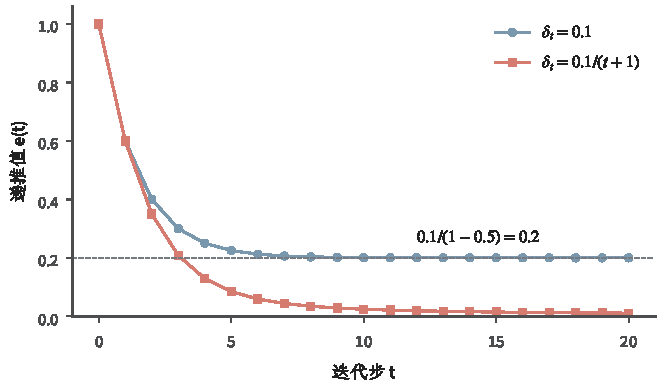
\includegraphics[width=\linewidth]{figures/01-mathematical-preliminaries/01-mathematical-language-combinatorics-analysis-optimization/matplotlib/analysis-geometry/language-perturbed-recurrence.pdf}
 \caption{相同初值与收缩系数下的两种递推。蓝线使用持续扰动，红线使用衰减扰动；每个点都是整数步上的精确递推值，图中$e(t)$对应正文的$e^{(t)}$，灰虚线是持续扰动留下的极限$0.2$。图为教学构造。}
 \label{fig:prelim-perturbed-recurrence}
\end{figure}

衰减扰动的结论可以直接由有限展开式~\eqref{eq:analysis-perturbed-distance-unrolling}核对。
给定$\varepsilon>0$，先选$S$使$s\geq S$时$\delta_s\leq\varepsilon(1-\rho)/2$。
对$t>S$把累计和拆成两段：前$S$项是有限个旧扰动，其权重随$t$几何趋零；后面的项满足
\[
 \sum_{s=S}^{t-1}\rho^{t-1-s}\delta_s
 \leq\frac{\varepsilon(1-\rho)}2\sum_{j=0}^{t-1-S}\rho^j
 \leq\frac\varepsilon2.
\]
旧扰动项和初始误差在充分大的$t$后也不超过$\varepsilon/2$，因此总误差趋于零。
这里需要$0\leq\rho<1$、$\delta_s\to0$和有限的初始误差；只写“每步误差很小”仍不足够。

\section{函数的连续性与局部变化}
\label{sec:analysis-local-models}

序列极限说明一族输入能否稳定；给定映射以后，还要判断这种稳定能否传到输出。
本节固定一个函数，分别考察输入扰动的控制、局部变化的计算及其近似误差。
由方程间接确定的函数需要额外证明解分支存在；经典可微性失效的函数则需要重新选择
变化信息。这些问题都针对函数本身，不要求先定义它的积分。

\subsection{连续性与扰动控制}
\label{sec:analysis-metric-continuity-extrema}

确定输入与输出的距离后，可以要求小的输入扰动只引起小的输出扰动。这就把熟悉的
实函数连续性推广到一般度量空间。
\Needspace{12\baselineskip}
\begin{definition}[度量空间中的连续映射]
\label{def:analysis-continuity}
设$(X,d_X)$与$(Y,d_Y)$为度量空间。函数$f:X\to Y$在$x\in X$处
\term{连续}（continuous），是指
\[
  \begin{gathered}
    \forall\varepsilon>0,\quad \exists\delta>0,\quad \forall x'\in X,\\
    d_X(x,x')<\delta\Longrightarrow d_Y\bigl(f(x),f(x')\bigr)<\varepsilon.
  \end{gathered}
\]
若$f$在每个$x\in X$处连续，则称$f$在$X$上连续。
\end{definition}
这里$\delta$可以依赖$x$和$\varepsilon$。等价地，只要$x_n\to x$，就有$f(x_n)\to f(x)$。连续函数因而允许把一个已经存在的极限送入函数：$f(\lim_n x_n)=\lim_n f(x_n)$。这里必须同时说明输入和输出采用的度量。

例如恒等映射$F(x)=x$从$(\mathbb R,d_1)$映到$(\mathbb R,d_2)$时处处不连续。
在任意$x$附近，总能找到通常距离任意小但不等于$x$的$x'$，它们的输出距离却始终为
$1$，无法小于$\varepsilon=1/2$。反过来，从$(\mathbb R,d_2)$到
$(\mathbb R,d_1)$的同一公式连续：选$\delta=1/2$，输入距离小于$\delta$就只可能
有$x'=x$，输出距离于是为$0$。这不是函数公式发生变化，而是输入输出空间对
“附近”的判断不同。图~\ref{fig:analysis-metric-convergence}右侧显示前一种失败。

\begin{figure*}[htbp]
  \centering
  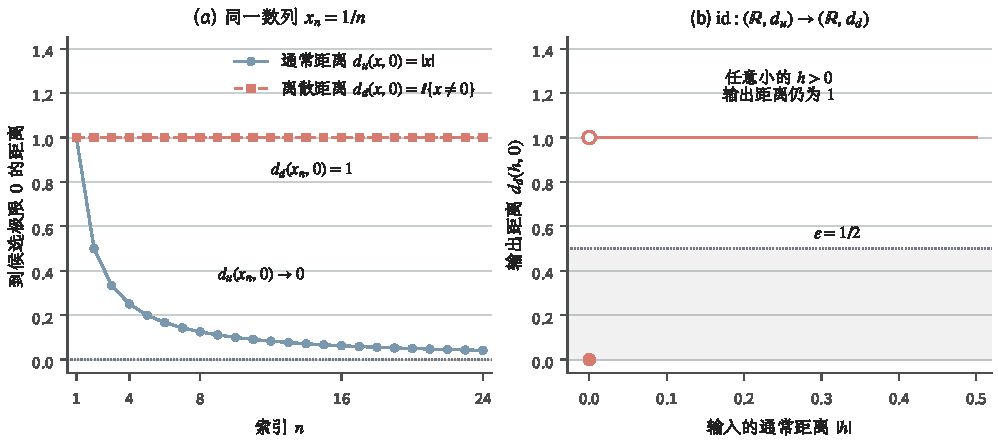
\includegraphics[width=\linewidth]{figures/01-mathematical-preliminaries/01-mathematical-language-combinatorics-analysis-optimization/matplotlib/analysis-concepts/analysis-metric-convergence.pdf}
  \caption{数值相同，距离不同。图中$d_u,d_d$分别对应正文的通常距离$d_1$与离散距离$d_2$。（a）数列 $x_n=1/n$ 到 $0$ 的通常距离趋于零，离散距离却恒为 $1$，所以收敛要连同度量说明。（b）恒等映射从通常度量空间映入离散度量空间时，任意非零且很小的输入位移仍对应输出距离 $1$，不能进入 $\varepsilon=1/2$ 的输出邻域，故它在 $0$ 处不连续。图为解析教学示例。}
  \label{fig:analysis-metric-convergence}
\end{figure*}

\begin{definition}[一致连续映射]
\label{def:analysis-uniform-continuity}
设$(X,d_X)$与$(Y,d_Y)$为度量空间，$f:X\to Y$。若对每个$\varepsilon>0$都能找到一个与具体位置无关的$\delta>0$，使任意
$x,x'\in X$只要$d_X(x,x')<\delta$便有
$d_Y(f(x),f(x'))<\varepsilon$，就称$f$\term{一致连续}
（uniformly continuous）。
\end{definition}
连续性允许不同位置使用不同的$\delta$，一致连续则要求同一个
$\delta$同时控制整个定义域。连续性本身并不足以给出这种统一控制：
$f(x)=x^2$在$\mathbb{R}$上连续，令$x\to+\infty$并取$x'=x+1/x$，可见输入距离趋于零而输出距离
$|f(x')-f(x)|=2+1/x^2$不趋于零。

\begin{definition}[Lipschitz连续映射]
\label{def:analysis-lipschitz-continuity}
设$(X,d_X)$与$(Y,d_Y)$为度量空间，$f:X\to Y$。若存在有限常数$L\geq0$，使所有$x,x'\in X$都满足
\begin{equation}
  d_Y\bigl(f(x),f(x')\bigr)\leq Ld_X(x,x'),
\label{eq:analysis-lipschitz-condition}
\end{equation}
则称$f$为$L$-\term{Lipschitz连续}（Lipschitz continuous）。
\end{definition}
它不仅用同一个
$\delta$控制整个定义域，还给出输出变化相对于输入变化的线性上界，因而蕴含一致连续。
函数$f(x)=\sqrt{x}$在$[0,1]$上满足$|\sqrt{x}-\sqrt{x'}|\leq\sqrt{|x-x'|}$，
因而选$\delta=\varepsilon^2$就得到一致连续性，却不能得到Lipschitz连续性：若存在有限$L$，
令$x'=0$便会要求$\sqrt{x}\leq Lx$，即$1/\sqrt{x}\leq L$，这在$x\downarrow0$时不可能成立。
同一个公式在不同定义域上可能具有不同的统一控制。$f(x)=x^2$在$[0,1]$上满足
$|x^2-z^2|\leq2|x-z|$，因而$2$-Lipschitz；在整个实线上却没有有限的全局Lipschitz
常数。这两个例子说明，统一的$\varepsilon$--$\delta$控制与线性误差上界仍是不同要求。

\term{局部Lipschitz函数}（locally Lipschitz function）要求每个点附近的函数变化
都能由某个有限Lipschitz常数控制。与全局Lipschitz条件不同，各个邻域可以使用不同的常数。
\begin{definition}[局部Lipschitz函数]
\label{def:analysis-local-lipschitz}
设$U\subseteq\mathbb{R}^d$为开集，$f:U\to\mathbb{R}$。若对每个$\bm{x}\in U$，
都存在半径$r>0$与有限常数$L\geq0$，使$B(\bm{x},r)\subseteq U$，并且
\[
  |f(\bm{y})-f(\bm{z})|
  \leq L\lVert\bm{y}-\bm{z}\rVert_2
  \quad\text{对所有 }\bm{y},\bm{z}\in B(\bm{x},r)\text{成立},
\]
则称$f$在$U$上局部Lipschitz。
\end{definition}

这里$r$与$L$可以依赖中心点；一旦邻域确定，同一个$L$须控制其中的任意两点。
例如$f(x)=x^2$在任意$(x_0-r,x_0+r)$上可取$L=2(|x_0|+r)$，所以在实轴上
局部Lipschitz，却不是全局Lipschitz。向量值函数也用输出范数替换绝对值，
作完全相同的局部定义。局部控制要提升为区域内的统一控制，还需要区域或导数的额外条件。


第~\ref{chap:sets-functions-and-proofs}章已区分下确界与最小值：数值可以逼近一个下界，却始终找不到达到它的点。
要让近似最优点最终提供一个可行解，需要防止点列逃向无穷远或被排除的边界。
在一般度量空间中，承担这一职责的是紧致性。
\begin{definition}[开覆盖与紧致性]
\label{def:analysis-compactness}
设$(X,d)$为度量空间，$K\subseteq X$。若一族$X$中的开集的并包含$K$，就称这族开集为$K$的
\term{开覆盖}（open cover）；若从中选出的有限个开集仍覆盖$K$，它们就构成
\term{有限子覆盖}（finite subcover）。集合$K$的每个开覆盖都能选出有限子覆盖时，
称$K$为\term{紧致}（compact）。
\end{definition}
在度量空间中，这一定义等价于
\term{序列紧致性}：集合中的每个序列都有一个子序列收敛到仍在该集合中的点。
后一种表述更适合分析算法产生的点列，因为它直接提供候选极限。

紧致性还能把逐点连续提升为一致连续：连续映射在紧致定义域上一定一致连续。
这为前面闭区间上的统一控制提供了一个一般条件，但不保证Lipschitz连续；
$\sqrt{x}$的例子已说明，输出变化未必能由输入距离的一次常数倍控制。

在有限维欧氏空间$\mathbb{R}^d$中，Heine--Borel定理说明紧致等价于闭且有界。这个结论不能原样搬到一般度量空间。考虑所有有界实数序列组成的空间
\[   \ell^\infty   =   \left\{\bm{x}=(x_1,x_2,\ldots):   \sup_{k\geq1}|x_k|<\infty\right\},   \qquad   d(\bm{x},\bm{y})=\sup_{k\geq1}|x_k-y_k|. \]
令$\bm{e}_n$只有第$n$个坐标为$1$，其余坐标为$0$。集合 $\{\bm{e}_n:n\geq1\}$有界，而且在$\ell^\infty$中是闭集；但$n\neq m$时 $d(\bm{e}_n,\bm{e}_m)=1$，所以任何子序列都不是柯西数列，更不可能收敛。一般空间中 “闭且有界”不足以替代紧致，正是因为无穷多个彼此分离的方向可能留在同一个有界球内。
\begin{theorem}[紧致集上的极值定理]
\label{thm:analysis-extreme-value}
设$K$是非空紧致度量空间，$f:K\to\mathbb{R}$连续，则$f$在$K$上同时达到最小值与最大值。
\end{theorem}
这里回顾熟悉的极值定理，不再展开证明。紧致性的两项作用是从近似最优点列中抽出收敛子序列，并保证极限仍在可行集合内。连续性随后把函数值极限传到该点。任一条件缺失都可能使最优解不存在。
\begin{example}[极值存在条件怎样失效]
\label{ex:analysis-extrema-failures}
在开区间$(0,1)$上，连续函数$f(x)=x$的下确界为$0$，却没有最小点；定义域不紧致， 极限点$0$被排除。把定义域改成闭但不紧致的$\mathbb{R}$，连续函数$f(x)=e^x$仍有下确界$0$而不达到它。另一方面，在紧致集合$[0,1]$上定义
\[   g(0)=1,\qquad g(x)=x\quad(x>0), \]
则$\inf g=0$也未达到；这次失败的是$g$在$0$处不连续。三个例子分别表明“连续”、 “闭”或“有界”中的单独一项都不是一般的极值存在保证。
\end{example}

连续性与可导性也应分开。回顾一元情形，导数要求左右两侧的差商趋向同一斜率，
比函数值趋近本身更强：$x^2$光滑，$|x|$在$0$连续但有尖点，
阈值函数$\mathbb I\{x\geq0\}$则在$0$跳跃。
尖点只阻止共同斜率，跳跃连共同的函数值极限也破坏了。
图~\ref{fig:analysis-continuity-counterexamples}把三者放在同一位置比较；
下一小节将写出差商和整体线性近似的正式条件。

\begin{figure*}[htbp]
  \centering
  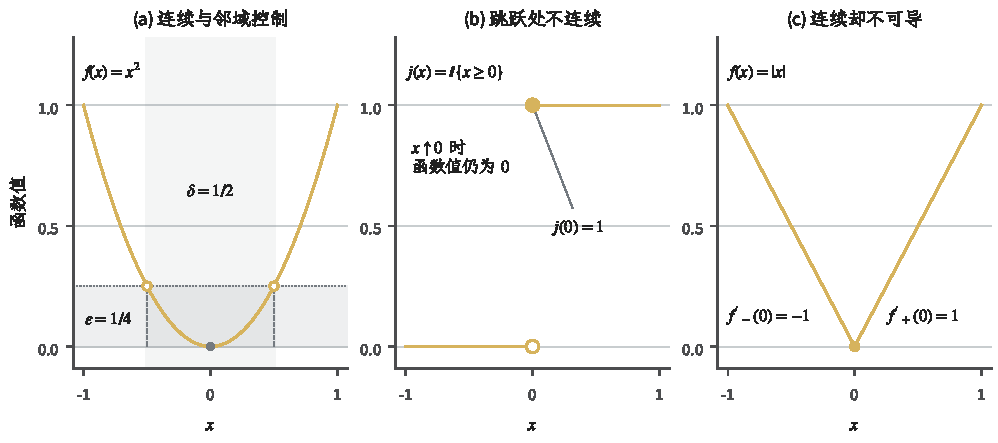
\includegraphics[width=\linewidth]{figures/01-mathematical-preliminaries/01-mathematical-language-combinatorics-analysis-optimization/matplotlib/analysis-concepts/analysis-continuity-counterexamples.pdf}
  \caption{三个不同的局部性质。（a）$f(x)=x^2$ 在 $0$ 处可用 $\delta=1/2$ 控制 $\varepsilon=1/4$：严格位于输入邻域内的点，其函数值严格落在输出邻域内。（b）阶跃函数在 $0$ 的左极限为 $0$，取值却为 $1$，空心点和实心点区分两者。（c）$|x|$ 在 $0$ 处连续，但左右导数分别为 $-1$ 和 $1$，不存在共同的双侧导数。图中曲线均为解析教学示例。}
  \label{fig:analysis-continuity-counterexamples}
\end{figure*}

\subsection{一阶导数与线性近似}
\label{sec:analysis-vector-chain-matrix-calculus}
\label{sec:analysis-derivatives-linear-approximation}
连续性只保证小扰动不会引起固定幅度的跳变；若还要预测变化的方向和大小，
就要寻找一个作用于扰动的线性映射。本节先建立这个近似，再处理不同输入输出形状：向量输出
需要Jacobian矩阵，复合映射需要串联两层线性变化，矩阵变量则需要用迹内积表示同一个
一阶变化。这里的“一阶”指对输入扰动保留线性项，与下一节研究斜率变化的二阶导数相对。

\subsubsection{导数与全微分}

从一元函数开始，把输出增量除以输入增量，得到这一小段上的平均变化率；
输入增量趋零后若仍有稳定值，就用它预测附近的输出。

一元函数$f:\mathbb{R}\to\mathbb{R}$在$x$处的\term{导数}（derivative）定义为
\[   f'(x)=\lim_{h\to0}\frac{f(x+h)-f(x)}{h}, \]
前提是这个双侧极限存在。它说明输入发生小变化$h$时，函数增量的一阶部分是$f'(x)h$：
\begin{equation}
  f(x+h)=f(x)+f'(x)h+o(|h|).
\label{eq:analysis-scalar-first-order}
\end{equation}
第~\ref{sec:comb-growth-scales}节的小$o$仍表示相对余项趋零，不过这里的趋向是$h\to0$：余项$r(h)$满足$r(h)/|h|\to0$，不只是$h$本身很小。导数存在必然推出函数在该点连续，但连续不保证可导，例如$|x|$在$0$处连续，左右导数却分别为 $-1$和$1$。
这也解释了图中尖点与跳跃的区别；两者都不能使用经典双侧导数，失效的层次却不同。

对$f:\mathbb{R}^d\to\mathbb{R}$，沿方向$\bm{v}\in\mathbb{R}^d$的
\term{方向导数}（directional derivative）是
\[   D_{\bm{v}}f(\bm{x})   =   \lim_{t\to0}   \frac{f(\bm{x}+t\bm{v})-f(\bm{x})}{t}. \]
取$\bm{v}$为第$j$个坐标方向$\bm{e}_j$，就得到\term{偏导数}
（partial derivative）$\partial f/\partial x_j$。方向导数只检查一条直线，而整体可微性要求所有小扰动共享同一个线性近似。

函数$f:\mathbb{R}^d\to\mathbb{R}$在$\bm{x}$处\term{可微}
（differentiable），是指存在一个线性映射 $A:\mathbb{R}^d\to\mathbb{R}$，使
\begin{equation}
  f(\bm{x}+\bm{h})
  =
  f(\bm{x})+A(\bm{h})+o(\lVert\bm{h}\rVert_2).
\label{eq:analysis-total-differentiability}
\end{equation}
线性部分$A(\bm h)$称为全微分，也记为$\mathrm df_{\bm x}(\bm h)$。
条件要求对任意趋零的非零扰动$\bm h$都有
$|f(\bm x+\bm h)-f(\bm x)-A(\bm h)|/\lVert\bm h\rVert_2\to0$，
而不是先固定一个方向，再允许误差控制随方向改变。
在欧氏空间中，每个这样的线性泛函都可写为 $A(\bm{h})=\langle\nabla f(\bm{x}),\bm{h}\rangle$，其中
\[   \nabla f(\bm{x})   =   \left(     \frac{\partial f}{\partial x_1}(\bm{x}),\ldots,     \frac{\partial f}{\partial x_d}(\bm{x})   \right)^{\top} \]
称为\term{梯度}（gradient）。因此梯度不是若干偏导数的随意排列，而是表示局部线性映射的向量；扰动$\bm{h}$通过内积变成函数的一阶变化。

可微必然推出所有方向导数存在，并且 $D_{\bm{v}}f(\bm{x})=\langle\nabla f(\bm{x}),\bm{v}\rangle$。反向结论不成立， 仅有偏导数更不够。
\begin{example}[偏导数存在但不可微]
\label{ex:analysis-partials-not-differentiable}
定义$f:\mathbb{R}^2\to\mathbb{R}$为
\[   f(x,y)=
\begin{cases}     \dfrac{xy}{\sqrt{x^2+y^2}}, & (x,y)\neq(0,0),\\[6pt]     0, & (x,y)=(0,0).
\end{cases} \]
沿两条坐标轴，函数恒为$0$，所以 $\partial f/\partial x(0,0)=\partial f/\partial y(0,0)=0$。若$f$在原点可微， 候选线性部分只能是零映射。可是沿$\bm{h}=(t,t)$，
\[   \frac{|f(t,t)-f(0,0)|}{\lVert(t,t)\rVert_2}   =   \frac{|t|/\sqrt{2}}{\sqrt{2}|t|}   =\frac12, \]
余项与$\lVert\bm{h}\rVert_2$之比不趋于零，故$f$在原点不可微。偏导数只看坐标轴，遗漏了其他接近路径。本例沿每个方向$\bm v=(a,b)$的
正向方向导数都存在，这里只令$t\downarrow0$，得到$ab/\sqrt{a^2+b^2}$（零方向取$0$）；它却不是关于$\bm v$
的线性函数，而且双侧方向导数在$ab\neq0$时不存在。方向极限采用单侧还是双侧，
必须与所用定义一致；本节定义采用双侧极限。
\end{example}

一个常用的充分条件是：若$f$的所有一阶偏导数在$\bm{x}$的某个邻域内存在，并在 $\bm{x}$处连续，则$f$在$\bm{x}$处可微。注意这只是方便核对的充分条件，不是必要条件； 可微函数的偏导数不一定在该点附近连续。

即使每个双侧方向导数都存在，也未必可微。例如令
$g(x,y)=x^3/(x^2+y^2)$于非零点，$g(0,0)=0$。
沿$\bm v=(a,b)\neq\bm0$有$D_{\bm v}g(0,0)=a^3/(a^2+b^2)$，
但坐标方向导数给出的候选梯度为$(1,0)^\top$，它对方向$(1,1)^\top$
预测$1$而非实际的$1/2$。这些方向变化率无法拼成一个线性映射。
与前例的单侧方向极限相比，这里直接检验了本节采用的双侧定义。

用$f(x)=x^3-3x$保留一个贯穿例子。在$x_0=1/2$处，
\[
  f(x_0)=-\frac{11}{8},\qquad f'(x_0)=3x_0^2-3=-\frac94.
\]
输入改变$h$时，一阶近似给出
\begin{equation}
  T_1(h)=f(x_0)+f'(x_0)h=-\frac{11}{8}-\frac94h.
\label{eq:analysis-cubic-linear-model}
\end{equation}
取$h=0.1$，$T_1(h)=-1.600$，而实际$f(0.6)=-1.584$。近似抓住了下降方向和主要
变化量，但还有$0.016$的误差；第~\ref{sec:analysis-second-order-curvature}节将用曲率解释这部分差别。
\subsubsection{复合映射与链式法则}

当一个输入产生多个输出时，每个输出都有一行局部线性系数，把这些行排在一起便得到
Jacobian矩阵。复合计算只需再把前一层的输出扰动作为后一层的输入扰动。
设$f:\mathbb{R}^d\to\mathbb{R}^m$。若存在矩阵 $\bm{J}_f(\bm{x})\in\mathbb{R}^{m\times d}$使
\begin{equation}
  f(\bm{x}+\bm{h})
  =
  f(\bm{x})+\bm{J}_f(\bm{x})\bm{h}
  +o(\lVert\bm{h}\rVert_2),
\label{eq:analysis-jacobian-linearization}
\end{equation}
则称$f$在$\bm{x}$处可微，$\bm{J}_f(\bm{x})$称为
\term{Jacobian矩阵}（Jacobian matrix）。其第$i,j$个元素是 $\partial f_i/\partial x_j$。矩阵有$m$行、$d$列，因为它把$d$维输入扰动映射成 $m$维输出扰动。

若$f$在$\bm{x}$处可微，且$g:\mathbb{R}^m\to\mathbb{R}^p$在$f(\bm{x})$处可微，则复合映射满足
\begin{equation}
  \bm{J}_{g\circ f}(\bm{x})
  =
  \bm{J}_g\bigl(f(\bm{x})\bigr)\bm{J}_f(\bm{x}).
\label{eq:analysis-vector-chain-rule}
\end{equation}
这就是\term{链式法则}（chain rule）。维度同时给出乘法次序： $(p\times m)(m\times d)=p\times d$，反向相乘往往没有定义。即使两个方阵能够交换书写顺序，矩阵乘法通常也不交换，不能据标量求导经验调换因子。

上面的$g$允许向量输出。当$p=1$时，$g$把中间向量变成一个标量。在优化问题中，
这个标量通常是待最小化的目标值，本书便把此时的$g$记为$\ell$。令
$\bm y=f(\bm x)$，总目标就是$L(\bm x)=\ell(f(\bm x))$；$\ell$只是原复合映射的
最后一层，并没有增加一个未说明的输出。采用列向量梯度，链式法则写成
\[
  \nabla L(\bm x)
  =\bm J_f(\bm x)^\top\nabla\ell(\bm y)\big|_{\bm y=f(\bm x)}.
\]
局部线性映射在前向计算中按$\bm J_f$作用，在标量目标的反向计算中按转置
$\bm J_f^\top$传回。这是后续反向传播的线性代数核心，具体网络结构留到模型章节。

\begin{example}[从中间向量求回复合目标的梯度]
\label{ex:analysis-chain-rule-calculation}
令
\[
  f(x_1,x_2)=(x_1^2,x_1x_2,x_2)^\top,
  \qquad \ell(\bm y)=\frac12(y_1^2+y_2^2+y_3^2).
\]
$f$从二维输入产生三维中间量，$\ell$再把三维中间量变成一个数。于是
\[
  \bm J_f=\begin{bmatrix}2x_1&0\\x_2&x_1\\0&1\end{bmatrix},
  \qquad \nabla\ell(\bm y)=\bm y.
\]
在$\bm x=(1,2)^\top$处，$\bm y=(1,2,2)^\top$，链式法则给出
\[
  \nabla L(1,2)
  =\begin{bmatrix}2&2&0\\0&1&1\end{bmatrix}
    \begin{bmatrix}1\\2\\2\end{bmatrix}
  =\begin{bmatrix}6\\4\end{bmatrix}.
\]
也可以把复合函数直接展开为
$L(x_1,x_2)=\tfrac12(x_1^4+x_1^2x_2^2+x_2^2)$，求偏导得到
$\nabla L=(2x_1^3+x_1x_2^2,\,x_1^2x_2+x_2)^\top$，在同一点仍为$(6,4)^\top$。
两种计算处理同一个目标；链式形式保留了中间映射，可分别复用各层的导数。
矩阵形状$(2\times3)(3\times1)=2\times1$也核对了梯度传递的次序。
\end{example}

若要把任意实数评分变成正数且总和为$1$的权重，可以先取指数再除以共同的总和。
这就是$n$维\term{归一化指数映射}（softmax）。对
$\bm{z}\in\mathbb{R}^n$，令
\[
  s_i(\bm{z})
  =
  \frac{e^{z_i}}{\sum_{k=1}^n e^{z_k}},
  \qquad i=1,\ldots,n.
\]
记分母为$Z=\sum_k e^{z_k}$。指数函数求导和商法则给出
\[
  \frac{\partial s_i}{\partial z_j}
  =
  \frac{\mathbb{I}\{i=j\}e^{z_i}Z-e^{z_i}e^{z_j}}{Z^2}
  =
  s_i\bigl(\mathbb{I}\{i=j\}-s_j\bigr).
\]
因此整个Jacobian矩阵为
\begin{equation}
  \bm{J}_{\bm{s}}(\bm{z})
  =
  \operatorname{diag}(\bm{s})-\bm{s}\bm{s}^{\top}.
\label{eq:analysis-softmax-jacobian}
\end{equation}
对角项$s_i(1-s_i)$描述提高$z_i$对自身分量的影响，非对角项$-s_is_j$
来自共同分母：提高一个坐标会压低其余归一化分量。每行元素之和为零，
这也与给所有$z_i$同时加同一常数不改变输出相符。
\subsubsection{矩阵变量与微分计算}

如果输入本身是矩阵，逐条写出$mn$个偏导数会掩盖原有的矩阵乘法结构。矩阵$\bm{X}\in\mathbb{R}^{m\times n}$可以看成$mn$个坐标组成的对象，矩阵梯度则把这些一阶变化重新排回原来的形状。先固定Frobenius迹内积
\[   \langle\bm{A},\bm{B}\rangle_F   =   \operatorname{tr}(\bm{A}^{\top}\bm{B}) \]
其中$\operatorname{tr}$是方阵对角元素之和，所以这个内积也等于
$\sum_{i,j}\bm A_{i,j}\bm B_{i,j}$，对应范数为
$\lVert\bm H\rVert_F=(\sum_{i,j}\bm H_{i,j}^2)^{1/2}$。
对标量函数$f(\bm X)$，全微分要求
$f(\bm X+\bm H)=f(\bm X)+\mathrm df_{\bm X}(\bm H)+o(\lVert\bm H\rVert_F)$。
用这个内积
定义矩阵梯度：若一阶全微分能够写成
\begin{equation}
  \mathrm{d}f
  =
  \langle\nabla_{\bm{X}}f,\mathrm{d}\bm{X}\rangle_F
  =
  \operatorname{tr}\bigl((\nabla_{\bm{X}}f)^{\top}
  \mathrm{d}\bm{X}\bigr),
\label{eq:analysis-matrix-gradient-definition}
\end{equation}
则$\nabla_{\bm{X}}f$与$\bm{X}$形状相同。计算时可先用乘积法则展开微分，再利用
\[   \operatorname{tr}(\bm{A}\bm{B})   =\operatorname{tr}(\bm{B}\bm{A}),\qquad   \operatorname{tr}(\bm{A}\bm{B}\bm{C})   =\operatorname{tr}(\bm{B}\bm{C}\bm{A}), \]
把$\mathrm{d}\bm{X}$移动到末端。迹只允许循环移位，不能任意交换相邻矩阵。

先考虑二次型$q(\bm{x})=\bm{x}^{\top}\bm{A}\bm{x}$，其中 $\bm{A}\in\mathbb{R}^{d\times d}$固定。由乘积法则，
\begin{align*}
  \mathrm{d}q
  &=
  (\mathrm{d}\bm{x})^{\top}\bm{A}\bm{x}
  +\bm{x}^{\top}\bm{A}\,\mathrm{d}\bm{x}\\
  &=
  \bm{x}^{\top}(\bm{A}^{\top}+\bm{A})\,\mathrm{d}\bm{x}.
\end{align*}
因此
\begin{equation}
  \nabla_{\bm{x}}
  \bigl(\bm{x}^{\top}\bm{A}\bm{x}\bigr)
  =
  (\bm{A}+\bm{A}^{\top})\bm{x}.
\label{eq:analysis-quadratic-form-gradient}
\end{equation}
只有当$\bm{A}$对称时才能化为$2\bm{A}\bm{x}$。直接写成$2\bm{A}\bm{x}$会悄然加入对称性条件。

对固定的$\bm{A}\in\mathbb{R}^{m\times n}$，令 $f(\bm{X})=\operatorname{tr}(\bm{A}^{\top}\bm{X})$。它的微分已经符合式
\eqref{eq:analysis-matrix-gradient-definition}，所以
\begin{equation}
  \nabla_{\bm{X}}\operatorname{tr}(\bm{A}^{\top}\bm{X})
  =\bm{A}.
\label{eq:analysis-trace-linear-gradient}
\end{equation}
这个简单关系常用于从迹表达式中读出梯度。

若方阵$\bm{X}$可逆，由恒等式$\bm{X}\bm{X}^{-1}=\bm{I}$取微分可得
\[   (\mathrm{d}\bm{X})\bm{X}^{-1}   +\bm{X}\,\mathrm{d}(\bm{X}^{-1})=\bm{0}. \]
左乘$\bm{X}^{-1}$后得到
\begin{equation}
  \mathrm{d}(\bm{X}^{-1})
  =
  -\bm{X}^{-1}(\mathrm{d}\bm{X})\bm{X}^{-1}.
\label{eq:analysis-inverse-differential}
\end{equation}
两个$\bm{X}^{-1}$位于扰动两侧，不能合并成 $-\bm{X}^{-2}\mathrm{d}\bm{X}$，因为$\mathrm{d}\bm{X}$未必与$\bm{X}^{-1}$交换。

最后设$\bm{X}\in\mathbb{R}^{d\times d}$正定，因而$\det\bm{X}>0$且 $\log\det\bm{X}$有定义。Jacobi行列式公式给出
\[   \mathrm{d}\det\bm{X}   =   \det(\bm{X})\operatorname{tr}   (\bm{X}^{-1}\mathrm{d}\bm{X}). \]
再应用标量对数的链式法则，
\begin{equation}
  \mathrm{d}\log\det\bm{X}
  =
  \operatorname{tr}(\bm{X}^{-1}\mathrm{d}\bm{X}),
  \qquad
  \nabla_{\bm{X}}\log\det\bm{X}
  =
  \bm{X}^{-\top}.
\label{eq:analysis-logdet-gradient}
\end{equation}
正定矩阵对称，所以$\bm{X}^{-\top}=\bm{X}^{-1}$；对一般可逆实矩阵， $\log\det\bm{X}$还需要$\det\bm{X}>0$，而梯度应保留转置。以上推导依赖的不是元素级记忆口诀，而是局部线性近似、乘积次序和迹内积三件事。
\begin{example}[逆矩阵微分中的乘法次序]
\label{ex:analysis-noncommuting-inverse-differential}
取$\bm X=\operatorname{diag}(2,1)$，扰动方向
$\bm E=\begin{bmatrix}0&1\\1&0\end{bmatrix}$。沿$\bm X+t\bm E$求逆矩阵的导数为
\[
 -\bm X^{-1}\bm E\bm X^{-1}
 =\begin{bmatrix}0&-1/2\\-1/2&0\end{bmatrix}.
\]
若照搬标量规则而写成$-\bm X^{-2}\bm E$，会得到
$\begin{bmatrix}0&-1/4\\-1&0\end{bmatrix}$，连对称性都丢失。
原路径在$0$附近由对称可逆矩阵组成，其逆与导数也应对称；这一结构检查能直接发现错误。
矩阵变量沿给定方向微分时，夹在两侧的逆矩阵不能随意移到同一侧。
\end{example}

\subsubsection{导数界与位移控制}

一点处的线性近似还不能控制一段有限位移。若沿整段路径的变化率都有上界，
中值定理才能把局部信息变成端点之间的误差界。
若$a<b$，$f:[a,b]\to\mathbb{R}$在$[a,b]$上连续、在$(a,b)$上可导，则
\term{中值定理}（mean value theorem）保证存在$c\in(a,b)$使
\begin{equation}
  f(b)-f(a)=f'(c)(b-a).
\label{eq:analysis-mean-value-theorem}
\end{equation}
所以，若区间上$|f'(x)|\leq L$，便有$|f(b)-f(a)|\leq L|b-a|$。这说明有界导数可以推出Lipschitz控制。多元标量函数也可沿线段使用一元中值定理：当连接 $\bm{x}$与$\bm{y}$的线段位于定义域且$f$在线段邻域可微时，
\[   |f(\bm{y})-f(\bm{x})|   \leq   \sup_{0\leq t\leq1}   \lVert\nabla f(\bm{x}+t(\bm{y}-\bm{x}))\rVert_2   \lVert\bm{y}-\bm{x}\rVert_2. \]
这里控制的是标量函数值差。对向量值函数，不能一般地断言存在一个共同的$c$让整个向量增量等于单个Jacobian矩阵乘以输入增量；应使用积分形式或范数上界。

对向量输出，用线性映射的最大放大倍数替代标量导数的绝对值。
\begin{definition}[欧氏诱导算子范数]
\label{def:analysis-induced-operator-norm}
对矩阵
$\bm{A}\in\mathbb{R}^{s\times r}$，由欧氏范数\term{诱导的算子范数}
（induced operator norm）定义为
\[
  \lVert\bm{A}\rVert_{\mathrm{op}}
  =
  \sup_{\bm{h}\neq\bm{0}}
  \frac{\lVert\bm{A}\bm{h}\rVert_2}{\lVert\bm{h}\rVert_2}
  =
  \sup_{\lVert\bm{h}\rVert_2=1}\lVert\bm{A}\bm{h}\rVert_2.
\]
\end{definition}
它表示线性映射对向量长度的最大放大倍数，定义立即给出
$\lVert\bm{A}\bm{h}\rVert_2
\leq\lVert\bm{A}\rVert_{\mathrm{op}}\lVert\bm{h}\rVert_2$。
例如$\bm A=\operatorname{diag}(2,1)$把第一坐标放大两倍、第二坐标保持不变，
故$\lVert\bm A\rVert_{\mathrm{op}}=2$；最大放大由第一坐标方向达到。
下文$\bm DG$与$\bm J_G$均表示$G$的Jacobian矩阵。
若映射$G$在包含$\bm{y}'$到$\bm{y}$线段的开邻域内连续可微，可以沿线段使用一元中值定理，得到
\begin{equation}
  \begin{aligned}
  \lVert G(\bm{y})-G(\bm{y}')\rVert_2
  &\leq
  \sup_{0\leq t\leq1}
  \left\lVert
    \bm{D}G\bigl(\bm{y}'+t(\bm{y}-\bm{y}')\bigr)
  \right\rVert_{\mathrm{op}}
  \lVert\bm{y}-\bm{y}'\rVert_2.
  \end{aligned}
\label{eq:analysis-operator-mean-value-bound}
\end{equation}
这个向量上界无需预先使用积分公式。若$\bm u=G(\bm y)-G(\bm y')\neq\bm0$，
取单位向量$\bm v=\bm u/\lVert\bm u\rVert_2$，并沿线段定义标量函数
$\phi(t)=\bm v^\top G(\bm y'+t(\bm y-\bm y'))$。
中值定理给出某个$\tau\in(0,1)$，使
\[
 \lVert\bm u\rVert_2
 =\phi(1)-\phi(0)
 =\bm v^\top\bm DG(\bm y'+\tau(\bm y-\bm y'))(\bm y-\bm y').
\]
对右侧使用欧氏内积与算子范数的上界便得到式~\eqref{eq:analysis-operator-mean-value-bound}；
$\bm u=\bm0$时该界直接成立。
因此，邻域内统一的导数范数上界会直接变成Lipschitz常数；若该上界小于$1$，就得到
第~\ref{sec:analysis-complete-contraction}节已经建立的压缩条件。

\subsection{二阶导数与局部曲率}
\label{sec:analysis-second-order-curvature}

延续$f(x)=x^3-3x$的例子，一阶导数$f'(x)=3x^2-3$还随位置变化。再求一次导数，
得到$f''(x)=6x$，所以$f''(1/2)=3$。在$x_0=1/2$附近，斜率向右移动时增大，
曲线向上弯；这解释了真实值为何高于前节的切线预测。图~\ref{fig:analysis-derivative-orders}将切线和下面的二次修正放在同一幅曲线图上比较。加入二次项得到
\begin{equation}
  T_2(h)=T_1(h)+\frac12f''(x_0)h^2
        =-\frac{11}{8}-\frac94h+\frac32h^2.
\label{eq:analysis-cubic-quadratic-model}
\end{equation}
在$h=0.1$时，$T_2=-1.585$，与实际值$-1.584$只差$0.001$。
一阶导数回答此处沿给定方向增还是减，二阶导数回答这个变化率怎样改变。
下一节再用Taylor展开给出一阶和二阶余项的完整表达式。

一阶近似只保留函数的局部斜率。若还要判断这个斜率怎样随位置改变，就需要
\term{Hessian矩阵}（Hessian matrix）。设$f:\mathbb{R}^d\to\mathbb{R}$在 $\bm{x}$附近二阶可微，定义
\[   \nabla^2 f(\bm{x})   =
\begin{bmatrix}     \dfrac{\partial^2 f}{\partial x_1^2} &     \cdots &     \dfrac{\partial^2 f}{\partial x_1\partial x_d}\\     \vdots & \ddots & \vdots\\     \dfrac{\partial^2 f}{\partial x_d\partial x_1} &     \cdots &     \dfrac{\partial^2 f}{\partial x_d^2}
\end{bmatrix}. \]
若二阶偏导数在邻域内连续，混合偏导数可以交换，Hessian矩阵因而对称。对方向 $\bm{v}$，二次型 $\bm{v}^{\top}\nabla^2f(\bm{x})\bm{v}$是沿直线 $t\mapsto f(\bm{x}+t\bm{v})$在$t=0$处的二阶导数。它衡量的不是函数值大小，而是沿该方向的一阶斜率变化。

对二次函数
\[   f(\bm{x})   =   \frac12\bm{x}^{\top}\bm{A}\bm{x}   +\bm{b}^{\top}\bm{x}+c, \]
只有$\bm{A}$的对称部分影响函数值。令 $\bm{H}=(\bm{A}+\bm{A}^{\top})/2$，则 $\nabla f(\bm{x})=\bm{H}\bm{x}+\bm{b}$且 $\nabla^2f(\bm{x})=\bm{H}$。正特征值对应向上弯曲的方向，负特征值对应向下弯曲的方向；特征值绝对值相差很大时，不同方向的尺度也相差很大。

\subsection{Taylor展开与余项控制}
\label{sec:analysis-taylor-approximation}
一阶导数给出切线，二阶导数描述斜率的变化，但近似不限于这两个阶数。Taylor展开
把函数在一点处的各阶导数组织成多项式，并用余项记录被舍弃的变化。
它承接前两节的导数计算，回答“保留多少信息能得到多准确的局部近似”，
而不把展开限定为二阶公式。

回顾一元Taylor公式：取非负整数$r$，若$f$在连接$x_0$与$x_0+h$的线段的开邻域上
$r+1$阶连续可微，且$h\neq0$，则存在两端之间的$\xi$使
\begin{equation}
  f(x_0+h)=\sum_{k=0}^{r}\frac{f^{(k)}(x_0)}{k!}h^k
  +\frac{f^{(r+1)}(\xi)}{(r+1)!}h^{r+1}.
\label{eq:analysis-taylor-arbitrary-order}
\end{equation}
约定$f^{(0)}=f$，$r$是所保留的最高次数。常数项记录当前函数值，线性项记录斜率，
二次项记录曲率，继续保留高阶项才得到更高阶近似。若沿这条线段
$|f^{(r+1)}|\leq M$，余项的绝对值便不超过$M|h|^{r+1}/(r+1)!$。
所以“高阶近似更准确”还依赖扰动尺度与导数上界，不能只比较多项式的次数。
此处给出的是选取某个中间点的Lagrange余项；若要保留整条线段上各位置的贡献，
第~\ref{sec:analysis-integration-remainders}节将由分部积分建立积分余项，
本节的极值判据并不依赖尚未建立的积分公式。

对前两节的$f(x)=x^3-3x$、$x_0=1/2$，三阶展开恰好为
\[
  f(x_0+h)=-\frac{11}{8}-\frac94h+\frac32h^2+h^3.
\]
此处所有四阶及以上导数为零，没有继续舍弃的项。一阶近似$T_1$与二阶近似$T_2$
分别舍弃$\tfrac32h^2+h^3$和$h^3$。图~\ref{fig:analysis-derivative-orders}把两侧扰动放在
同一尺度上比较，显示线性、二次近似怎样接近原曲线，并标出$h=\pm0.1$时的余项。

\begin{figure*}[htbp]
  \centering
  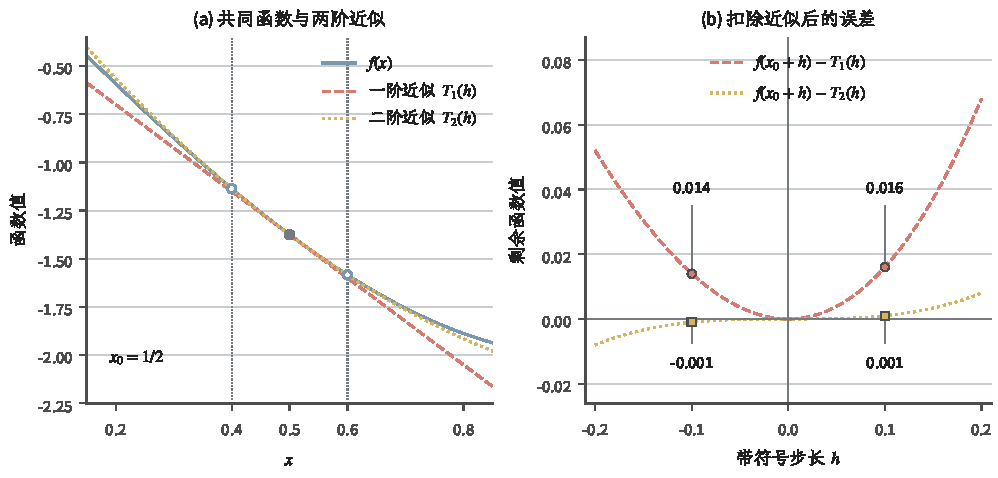
\includegraphics[width=\linewidth]{figures/01-mathematical-preliminaries/01-mathematical-language-combinatorics-analysis-optimization/matplotlib/analysis-concepts/analysis-derivative-orders.pdf}
  \caption{统一函数 $f(x)=x^3-3x$ 在 $x_0=1/2$ 处的两阶近似，记 $h=x-x_0$。（a）蓝线为真函数，红虚线为切线近似 $T_1=f(x_0)+f'(x_0)h$，黄点线加入二次项 $f''(x_0)h^2/2$，得到 $T_2$。（b）扣除各近似后的带符号余项分别为 $3h^2/2+h^3$ 与 $h^3$，标出 $h=\pm0.1$ 的精确结果。一阶导数确定切线，二阶导数补充局部曲率；余项的正负表示真值位于近似值的哪一侧。图为解析教学示例。}
  \label{fig:analysis-derivative-orders}
\end{figure*}


设连接$\bm{x}$与$\bm{x}+\bm{h}$的线段包含在一个开集内，并且$f$在该开集上二阶连续可微。对一元函数$\phi(t)=f(\bm{x}+t\bm{h})$使用Taylor定理，存在 $\theta\in(0,1)$使
\begin{equation}
  f(\bm{x}+\bm{h})
  =
  f(\bm{x})
  +\nabla f(\bm{x})^{\top}\bm{h}
  +\frac12
  \bm{h}^{\top}
  \nabla^2f(\bm{x}+\theta\bm{h})
  \bm{h}.
\label{eq:analysis-second-order-taylor}
\end{equation}
由Hessian矩阵的连续性，当$\bm{h}\to\bm{0}$时，中间点处的二阶项可以换成基点处的
二阶项，并把差异归入更小阶的余项：
\begin{equation}
  f(\bm{x}+\bm{h})
  =
  f(\bm{x})
  +\nabla f(\bm{x})^{\top}\bm{h}
  +\frac12\bm{h}^{\top}\nabla^2f(\bm{x})\bm{h}
  +o(\lVert\bm{h}\rVert_2^2).
\label{eq:analysis-second-order-local-model}
\end{equation}
式~\eqref{eq:analysis-second-order-local-model}是局部结论。若要在一个区域内给出统一余项界，还需控制该区域上的Hessian矩阵连续性或Lipschitz常数，不能仅凭一点处的二阶导数。


有了余项控制，才能由近似多项式判断函数本身的极值。局部极小点是指某个邻域内
所有函数值都不小于该点的值；严格局部极小还要求其他点的值严格更大。
设$\bm{x}^{\star}$是开集内部的局部极小点，且$f$在该点可微。对每个方向 $\bm{v}$考察$f(\bm{x}^{\star}+t\bm{v})$，一元函数的必要条件给出 $\nabla f(\bm{x}^{\star})^{\top}\bm{v}=0$。这对所有$\bm{v}$成立，因此
\begin{equation}
  \nabla f(\bm{x}^{\star})=\bm{0}.
\label{eq:analysis-first-order-necessary}
\end{equation}
若$f$还在该点二阶可微，同样沿任意方向使用一元二阶必要条件，可得
\begin{equation}
  \bm{v}^{\top}\nabla^2f(\bm{x}^{\star})\bm{v}\geq0
  \quad\text{对所有 }\bm{v},
\label{eq:analysis-second-order-necessary}
\end{equation}
即Hessian矩阵半正定。局部极大点对应半负定。这些只是必要条件：
$f(x)=x^4$与$f(x)=-x^4$在$0$处分别有严格局部极小值和严格局部极大值，
二者的二阶导数却都为零；$f(x)=x^3$在$0$处的一阶导数和二阶导数也都为零，
却没有极值。Hessian矩阵半正定或半负定本身不能决定驻点类型。

正定Hessian矩阵给出更强的充分条件。若$f$在$\bm{x}^{\star}$的某个邻域内二阶连续
可微，$\nabla f(\bm{x}^{\star})=\bm{0}$且
$\nabla^2f(\bm{x}^{\star})$正定，则其最小特征值为某个$\lambda>0$。由Hessian矩阵的
连续性，充分靠近$\bm{x}^{\star}$时，任意方向上的二次型仍至少为
$(\lambda/2)\lVert\bm{h}\rVert_2^2$。用式~\eqref{eq:analysis-second-order-taylor}
的中间点表达式，即可把这个曲率下界变成函数值下界；具体地，充分靠近时有
\[   f(\bm{x}^{\star}+\bm{h})-f(\bm{x}^{\star})   \geq   \frac{\lambda}{4}\lVert\bm{h}\rVert_2^2>0 \]
对充分小的非零$\bm{h}$成立，故$\bm{x}^{\star}$是严格局部极小点。负定情形给出严格局部极大点。

若驻点处Hessian矩阵既有正特征值又有负特征值，沿相应特征向量的小扰动会使函数值分别增加和减小，该点称为\term{鞍点}（saddle point）。例如 $f(x,y)=x^2-y^2$的原点就是鞍点。若Hessian矩阵仅半正定或含零特征值，二阶判据可能没有结论，必须查看更高阶项或函数的其他结构。上述必要条件还假定点位于无约束开集内部； 边界极小点的梯度可以不为零，受约束问题需要后续章节的可行方向与乘子条件。

\subsection{隐函数与解的敏感性}
\label{sec:analysis-implicit-parameter-integral}

链式法则计算已给定映射的变化；方程$F(\bm x,\bm y)=\bm0$却还没有直接给出
$\bm y$关于$\bm x$的函数。需要先证明局部解分支存在、唯一且可微，才能对它求导。
前面的导数位移界与本章压缩定理现在共同提供这一保证；驻点方程随后把解分支用于
参数变化下的敏感性分析。

显式关系$y=\varphi(x)$直接给出输入如何映射到输出，方程 $F(x,y)=0$却只规定二者必须共同满足的约束。例如 $F(x,y)=y^2-x=0$在$x>0$附近有$y=\sqrt{x}$和$y=-\sqrt{x}$两支，若不先指定所考察的解，方程并不定义唯一函数。更糟的是，在$(x,y)=(0,0)$附近，两支相交且 $\partial F/\partial y=2y=0$，不能把$y$稳定地看作$x$的可微函数。

\begin{theorem}[隐函数定理]
\label{thm:analysis-implicit-function}
设$F:\mathbb{R}^p\times\mathbb{R}^m\to\mathbb{R}^m$在 $(\bm{a},\bm{b})$的某个开邻域内连续可微， $F(\bm{a},\bm{b})=\bm{0}$，并且关于待解变量的Jacobian矩阵 \[   \bm{D}_{\bm{y}}F(\bm{a},\bm{b})   \in\mathbb{R}^{m\times m} \]
可逆。则存在$\bm{a}$与$\bm{b}$的邻域$U,V$，以及唯一的连续可微函数
$\varphi:U\to V$，使$\varphi(\bm{a})=\bm{b}$，并且对所有
$(\bm{x},\bm{y})\in U\times V$都有
\[
  F(\bm{x},\bm{y})=\bm{0}
  \quad\Longleftrightarrow\quad
  \bm{y}=\varphi(\bm{x}).
\]
其Jacobian矩阵满足
\begin{equation}
  \bm{D}\varphi(\bm{x})
  =
  -
  \bigl[\bm{D}_{\bm{y}}F(\bm{x},\varphi(\bm{x}))\bigr]^{-1}
  \bm{D}_{\bm{x}}F(\bm{x},\varphi(\bm{x})).
\label{eq:analysis-implicit-derivative}
\end{equation}
\end{theorem}

\begin{proof}
为证明定理~\ref{thm:analysis-implicit-function}的存在性，先把方程改写为局部压缩迭代。记
\[   \bm{A}   =   \bm{D}_{\bm{y}}F(\bm{a},\bm{b}),   \qquad   T_{\bm{x}}(\bm{y})   =   \bm{y}-\bm{A}^{-1}F(\bm{x},\bm{y}). \]
$F(\bm{x},\bm{y})=\bm{0}$当且仅当$\bm{y}$是$T_{\bm{x}}$的不动点。并且
\[   \bm{D}_{\bm{y}}T_{\bm{x}}(\bm{y})   =   \bm{I}   -   \bm{A}^{-1}\bm{D}_{\bm{y}}F(\bm{x},\bm{y}), \]
它在$(\bm{a},\bm{b})$处为零。由导数连续性，可以选择闭球 $B=\{\bm{y}:\lVert\bm{y}-\bm{b}\rVert_2\leq r\}$和$\bm{a}$的邻域$U$，使
\begin{equation}
  \sup_{\bm{x}\in U,\,\bm{y}\in B}
  \left\lVert
    \bm{D}_{\bm{y}}T_{\bm{x}}(\bm{y})
  \right\rVert_{\mathrm{op}}
  \leq q<1.
\label{eq:analysis-ift-uniform-contraction}
\end{equation}
沿$\bm{y}$方向使用式~\eqref{eq:analysis-operator-mean-value-bound}可知，每个
$T_{\bm{x}}$在$B$上都是同一因子$q$的压缩映射。

还必须核对自映射。因为$T_{\bm{a}}(\bm{b})=\bm{b}$且$T_{\bm{x}}(\bm{b})$关于 $\bm{x}$连续，可进一步缩小$U$，使
\[   \lVert T_{\bm{x}}(\bm{b})-\bm{b}\rVert_2   \leq\frac{1-q}{2}r. \]
于是对$\bm{y}\in B$，
\[
  \lVert T_{\bm{x}}(\bm{y})-\bm{b}\rVert_2
  \leq
  q\lVert\bm{y}-\bm{b}\rVert_2+\frac{1-q}{2}r
  \leq
  \frac{1+q}{2}r
  <r.
\]
所以$T_{\bm{x}}(B)$包含在$B$的内部$V$中。闭球$B$在有限维欧氏空间中完备，Banach
定理便对每个$\bm{x}\in U$给出唯一不动点$\varphi(\bm{x})\in V$。若
$(\bm{x},\bm{y})\in U\times V$且$F(\bm{x},\bm{y})=\bm{0}$，则$\bm{y}\in B$也是
$T_{\bm{x}}$的不动点，唯一性迫使$\bm{y}=\varphi(\bm{x})$。这证明了定理所述的局部
存在与零点集合的逐点唯一性。

还需说明所得解随参数连续可微。把$U$进一步缩小为开球，并使
$\overline U\times B$包含在原定义域内；这个集合紧致，关于$\bm x$的导数连续，
故有统一范数上界$L$。对$\bm x,\bm x'\in U$，
两点间的线段仍在$U$内，式~\eqref{eq:analysis-operator-mean-value-bound}
可用于$T_{\bm x}(\bm y)$的参数变化。利用两个不动点关系，
\[   \lVert\varphi(\bm{x})-\varphi(\bm{x}')\rVert_2   \leq   q\lVert\varphi(\bm{x})-\varphi(\bm{x}')\rVert_2   +L\lVert\bm{x}-\bm{x}'\rVert_2, \]
移项得到$\lVert\varphi(\bm x)-\varphi(\bm x')\rVert_2
\leq L\lVert\bm x-\bm x'\rVert_2/(1-q)$，
故$\varphi$局部Lipschitz连续。令 $\bm{h}\to\bm{0}$并记 $\bm{k}=\varphi(\bm{x}+\bm{h})-\varphi(\bm{x})$，前述界给出 $\lVert\bm{k}\rVert_2=O(\lVert\bm{h}\rVert_2)$。对恒等式
\[   F(\bm{x}+\bm{h},\varphi(\bm{x})+\bm{k})   -   F(\bm{x},\varphi(\bm{x}))   =   \bm{0} \]
作一阶展开，得到
\[   \bm{D}_{\bm{x}}F\,\bm{h}   +   \bm{D}_{\bm{y}}F\,\bm{k}   +   o(\lVert\bm{h}\rVert_2)   =   \bm{0}. \]
展开中的Jacobian均在$(\bm x,\varphi(\bm x))$处取值，联合扰动的余项
$o(\lVert(\bm h,\bm k)\rVert_2)$因$\lVert\bm k\rVert_2=O(\lVert\bm h\rVert_2)$
成为$o(\lVert\bm h\rVert_2)$。
基点的$\det\bm A\neq0$，行列式又是矩阵元素的连续函数，
所以邻域足够小时$\bm D_{\bm y}F$仍可逆。于是
\[   \bm{k}   =   -   (\bm{D}_{\bm{y}}F)^{-1}   \bm{D}_{\bm{x}}F\,\bm{h}   +   o(\lVert\bm{h}\rVert_2). \]
这证明$\varphi$可微并给出式~\eqref{eq:analysis-implicit-derivative}；各Jacobian矩阵连续又保证$\bm{D}\varphi$连续。至此，隐函数定理中的存在、局部唯一与导数公式都已得到说明。证明中特别核对了自映射和统一压缩条件，只有形式上的固定点改写并不足够。
\end{proof}

存在性、局部唯一性和可微性都需要证明，不能由形式求导代替。上面的证明已经核对这些条件。只看导数公式时，对恒等式 $F(\bm{x},\varphi(\bm{x}))=\bm{0}$应用链式法则，得到
\[   \bm{D}_{\bm{x}}F   +   \bm{D}_{\bm{y}}F\,\bm{D}\varphi   =   \bm{0}. \]
左乘$\bm{D}_{\bm{y}}F$的逆即得式~\eqref{eq:analysis-implicit-derivative}。乘法次序由矩阵维度决定，不能把逆矩阵随意移到右侧。


考虑依赖参数$\theta$的无约束目标$q(z,\theta)$。若局部最优解$z^\star(\theta)$位于定义域内部，它满足驻点方程
\[   F(\theta,z)   =   \frac{\partial q}{\partial z}(z,\theta)   =   0. \]
若$q$二阶连续可微，且 $\partial^2q/\partial z^2$在所考察解处非零，隐函数定理给出该驻点的局部唯一分支。这并不自动说明它是全局最优解；还要由曲率或其他结构核对最优性。
\begin{example}[参数二次目标中的解导数与包络导数]
\label{ex:analysis-parametric-quadratic}
对$\theta>-1$，令
\[   q(z,\theta)   =   \frac12(1+\theta)z^2-\theta z. \]
因为$\theta>-1$，配方得到
\[
  q(z,\theta)=\frac{1+\theta}{2}
  \left(z-\frac{\theta}{1+\theta}\right)^2
  -\frac{\theta^2}{2(1+\theta)}.
\]
平方项的系数为正，所以唯一驻点就是全局最小点。驻点方程为
\[   F(\theta,z)=(1+\theta)z-\theta=0. \]
隐式求导给出
\[   \frac{\mathrm{d}z^\star}{\mathrm{d}\theta}   =   -\frac{\partial F/\partial\theta}{\partial F/\partial z}   =   -\frac{z^\star-1}{1+\theta}. \]
直接消元得到
\[   z^\star(\theta)=\frac{\theta}{1+\theta},   \qquad   \frac{\mathrm{d}z^\star}{\mathrm{d}\theta}   =   \frac{1}{(1+\theta)^2}, \]
两种计算一致。

最优值$V(\theta)=q(z^\star(\theta),\theta)$的链式求导为
\[   V'(\theta)   =   \frac{\partial q}{\partial z}   \frac{\mathrm{d}z^\star}{\mathrm{d}\theta}   +   \frac{\partial q}{\partial\theta}. \]
在内部驻点，第一项因$\partial q/\partial z=0$消失，所以
\begin{equation}
  V'(\theta)
  =
  \left.
  \frac{\partial q}{\partial\theta}
  \right|_{z=z^\star(\theta)}
  =
  \frac12(z^\star)^2-z^\star.
\label{eq:analysis-envelope-quadratic}
\end{equation}
另一方面，直接代回可得
\[   V(\theta)=-\frac{\theta^2}{2(1+\theta)},   \qquad   V'(\theta)   =   -\frac{\theta(\theta+2)}{2(1+\theta)^2}, \]
与式~\eqref{eq:analysis-envelope-quadratic}一致。
\end{example}

式~\eqref{eq:analysis-envelope-quadratic}体现了\term{包络定理}
（envelope theorem）的基本机制：最优值的一阶变化不需要显式乘上最优解导数，因为目标对决策变量的一阶导数在内部最优点为零。但解导数本身并未消失；若关心参数变化后 $z^\star$怎样移动，仍要使用隐式求导。边界解、不可微目标、多重最优解或受约束问题不能直接套用这个简单版本，后续最优化章节会加入相应条件。

\subsection{非光滑函数与广义梯度}
\label{sec:analysis-nonsmooth-surrogate-gradient}
前面的微分公式都有可微性条件。遇到尖点、阈值或离散选择时，需要重新判断所使用的
变化信息：真实导数在何处存在，哪些广义导数仍有数学含义，算法又可能另外指定什么
更新信号。下面从真实函数的性质进入广义梯度，再区分人为替代规则，避免把三者混写。

函数$|x|$在$x\neq0$处导数为$\operatorname{sign}(x)$，在$0$处左右导数不同。
ReLU函数$\max\{0,x\}$把负输入截为零、正输入保持不变，也只在$0$处不可微。
由于单点是Lebesgue零测集，它们都几乎处处可导，但“几乎处处有导数”并没有为例外点指定导数值。

阈值函数$\mathbb{I}\{x\geq0\}$在$x\neq0$处导数为$0$，在$0$处不连续且不可微。若机械地使用几乎处处导数，反向传播得到的信号几乎处处为零，这无法表达跨过阈值会改变输出。重置、取整和离散选择也有类似问题：前向映射的真实局部导数可能不存在或不能提供有用方向。

凸函数的不可微点可以用凸次梯度处理，其正式定义与最优性条件见
第~\ref{sec:opt-subgradient-methods}节。凸次梯度依赖全局仿射下界，并非“随便给不可微点填
一个导数”；对于一般非凸函数，还需要区分其他广义导数概念。

定义~\ref{def:analysis-local-lipschitz}已经给出局部Lipschitz条件。Rademacher定理说明，满足该条件的函数关于Lebesgue测度几乎处处可微；这里回用第~\ref{sec:analysis-set-structures}节的零测集约定，定理仍没有为例外点指定唯一梯度。

一种适用于局部Lipschitz函数的扩展是\term{Clarke广义梯度}
（Clarke generalized gradient）：它收集从邻近可微点趋近时出现的梯度极限，再由这些
向量构成一组候选方向。非负权重且权重和为$1$的有限加权平均称为凸组合；允许所有这样
的组合，并纳入这些组合能够逼近的极限向量，就得到闭凸包。
\begin{definition}[Clarke广义梯度]
\label{def:analysis-clarke-generalized-gradient}
设$U\subseteq\mathbb{R}^d$为开集，$f:U\to\mathbb{R}$局部Lipschitz。对内点
$\bm{x}\in U$，$f$在$\bm{x}$处的Clarke广义梯度定义为
\[
  \partial^\circ f(\bm{x})
  =
  \overline{\operatorname{conv}}
  \left\{
    \lim_{k\to\infty}\nabla f(\bm{x}_k):
    \begin{array}{l}
      \bm{x}_k\in U,\quad\bm{x}_k\to\bm{x},\\
      f\text{在每个 }\bm{x}_k\text{处可微},\\
      \text{且上述梯度极限存在}
    \end{array}
  \right\}.
\]
其中$\operatorname{conv}$表示取所有有限凸组合，横线表示在$\mathbb{R}^d$中取闭包，
即把集合内序列的所有极限点也纳入。
\end{definition}
对局部Lipschitz凸函数，Clarke广义梯度与
第~\ref{sec:opt-subgradient-methods}节定义的凸次梯度集合一致；对一般非凸局部Lipschitz
函数，前者仍由邻近可微点的梯度极限构造，不再表示全局仿射下界。阈值函数在跳点附近
不连续，因而不是局部Lipschitz函数，不能直接套用这一构造。
例如$f(x)=-|x|$在原点左右两侧的导数分别为$1$与$-1$，故其Clarke广义梯度
是$[-1,1]$，包含零；然而原点是局部最大点。若把凸次梯度的全局下界定义硬用于此处，
正半轴要求斜率$g\leq-1$，负半轴却要求$g\geq1$，不存在满足条件的$g$。
同样的候选区间$[-1,1]$，在$|x|$上可以刻画全局最小点，在$-|x|$上却不提供这样的
保证。这说明广义梯度中含零只是相应的驻点条件，仍要核对所用定义和函数结构。
图~\ref{fig:analysis-clarke-stationarity-boundary}选取两者共有的候选$g=0$。
在$|x|$中，它给出有效的全局下界；在$-|x|$中，原函数反而处处不高于这条线。
局部斜率的凸包抹去了两边斜率出现的次序，不能替代函数整体上下关系。
\begin{figure*}[htbp]
 \centering
 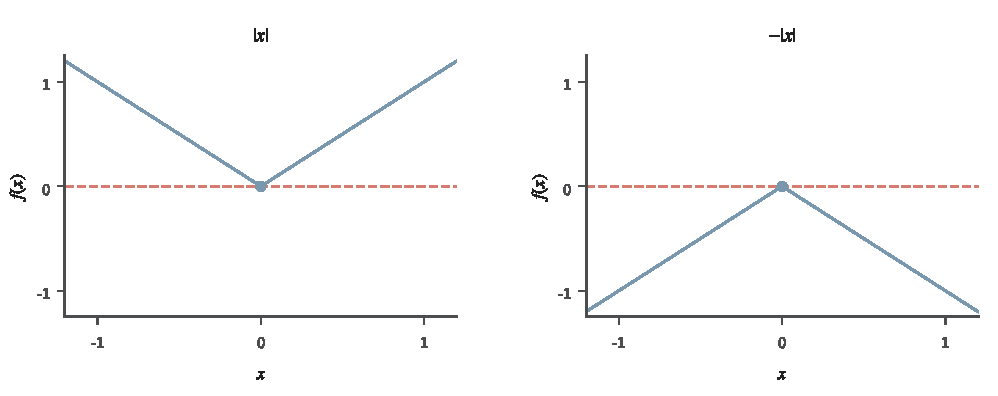
\includegraphics[width=\linewidth]{figures/01-mathematical-preliminaries/01-mathematical-language-combinatorics-analysis-optimization/matplotlib/teaching-analysis/analysis-clarke-stationarity-boundary.pdf}
 \caption{同一广义驻点条件的不同含义。蓝线分别为$|x|$与$-|x|$，红虚线为原点处候选斜率$g=0$对应的直线。
 两图在原点的Clarke广义梯度均为$[-1,1]$，却分别形成局部最小点与局部最大点；只有左图红线是全局仿射下界。
 两图共用坐标尺度，由解析式生成。}
 \label{fig:analysis-clarke-stationarity-boundary}
\end{figure*}



在含阈值或脉冲事件的模型中，常保留离散前向映射，却在反向计算时把其导数替换成某个平滑且非零的函数。这种信号称为\term{替代梯度}（surrogate gradient）。它是算法人为指定的近似更新方向，不自动等于前向映射的经典导数，也通常不满足凸次梯度的不等式。因此使用时应分别写清前向函数、反向替代函数及其尺度，不能把训练规则描述成对原离散函数的精确求导。

中心差分
\[   \frac{f(x+\varepsilon)-f(x-\varepsilon)}{2\varepsilon} \]
只能检验实际代入的函数$f$在尺度$\varepsilon$附近怎样变化。若程序反向传播使用替代梯度，而数值差分计算离散前向函数，两者本来就不是同一个导数对象；不一致不必然说明程序实现错误。

\section{函数的可测性与整体关系}
\label{sec:analysis-integration-average}

局部变化研究一个位置附近的输出增量；整体累计还要知道每个范围占多少权重。
第~\ref{sec:analysis-set-structures}节已建立可测集合族与测度，现在把函数的取值
与这些范围连接起来：可测性保证按取值分组后仍能赋权，积分再把每组贡献累计为总量。
整体关系还包括变量之间怎样共同累计，以及局部导数怎样转化为边界贡献。

\subsection{函数的可测性}

测度只知道集合的大小，还不知道函数在集合上贡献多少。把函数按取值分组后，每组
贡献就是“该取值乘以这组的测度”。因此，在写积分之前，要保证这些取值集合属于
已经允许测量的范围。

可测性说的是函数与这些测量范围是否相容：对输出值提出一个可测的条件，满足条件的
输入也应组成可测集合。这里需要的是集合的原像，并不要求函数有逆函数。
\begin{definition}[可测函数]
\label{def:analysis-measurable-function}
给定可测空间$(X,\mathcal{A})$与$(Y,\mathcal{B})$。若映射$f:X\to Y$满足
\[
  B\in\mathcal{B}\quad\Longrightarrow\quad
  f^{-1}(B)=\{x\in X:f(x)\in B\}\in\mathcal{A},
\]
则称$f$为从$(X,\mathcal{A})$到$(Y,\mathcal{B})$的\term{可测函数}
（measurable function）。对取值于$\mathbb{R}$或$\overline{\mathbb{R}}=[-\infty,\infty]$
的函数，目标空间取Borel $\sigma$代数；此时可测性等价于
\[
  \{x\in X:f(x)>a\}\in\mathcal{A}
  \qquad\text{对每个 }a\in\mathbb{R}\text{成立}.
\]
\end{definition}
阈值条件之所以足够，是因为这些半直线能生成目标空间的Borel $\sigma$代数，而原像
保持补集与可数并。它保证按函数值分层得到的集合都能取得测度。可测性依赖指定的
$\sigma$代数，并不依赖这些集合具体有多大权重。例如在$X=\{a,b\}$上只允许
$\mathcal{A}=\{\varnothing,X\}$时，$f(a)=0$、$f(b)=1$不可测：阈值$1/2$选出
$\{b\}$，不在$\mathcal{A}$中。把$\mathcal{A}$改为所有子集后，同一个函数就可测。

连续性比较输入与输出的距离，本身不以可测性为先决条件。若两端采用Borel $\sigma$代数，连续映射自动可测，因为开集的原像仍是开集；若任意指定其他$\sigma$代数，则不能只凭连续性保证可测。反向也不成立。
例如$[0,1]$上有理数的指示函数$\mathbb{I}_{\mathbb{Q}\cap[0,1]}$可测，因为有理数
集合是可数个单点的并，但它在每一点都不连续：任意小邻域内同时有有理数和无理数，
函数值在$1$和$0$之间跳变。可测性只保证取值分组可以测量，不保证图像平滑，
也不保证积分有限。可测函数列的逐点极限存在时仍可测，可数族可测函数的逐点上确界
和下确界也可测。这些封闭性使下面的阶梯逼近能够留在同一套积分框架中。

这些极限的可测性可以直接回到集合运算，而不依赖尚未建立的积分定理。对可测实函数列，
\begin{align*}
 \{x:\sup_n f_n(x)>a\}&=\bigcup_n\{x:f_n(x)>a\},\\
 \{x:\inf_n f_n(x)<a\}&=\bigcup_n\{x:f_n(x)<a\}.
\end{align*}
因此上确界、下确界可测；再用
$\liminf_n f_n=\sup_N\inf_{n\geq N}f_n$，得到下极限可测，逐点极限存在时就是它。
有限加法、绝对值、最大值等连续运算也保持实函数的可测性：
$(f,g)$的矩形原像是两个可测原像的交，而实平面的开集可写成可数个有理端点矩形的并。
这为后面按$\{f>a\}$分层、取正负部分和比较$f,g$提供了集合依据。

例如在$X=\mathbb R$上采用通常距离，却只允许
$\mathcal A=\{\varnothing,\mathbb R\}$，目标采用Borel集合族，则连续函数$f(x)=x$
不是从$(X,\mathcal A)$到目标可测空间的可测函数：开区间$(0,1)$的原像不属于
$\mathcal A$。因此可测、连续与可积需要分别核对其结构与条件。
即使固定Lebesgue测度，连续也不等于可积：$f(x)=1/x$在$(0,1)$上连续且可测，
总积分却为无穷。相反，有理数指示函数虽处处不连续，积分却为零。
下面构造积分后，再核对这些大小关系；可测性负责“能否按取值赋权”，可积性负责
“绝对贡献是否有限”。

\subsection{积分的构造与可积性}
\subsubsection{简单函数与非负积分}
一般函数可能取无穷多个不同的值，先从只取有限多个值的可测函数开始。它们可以按
每个取值对应的集合分组，使积分直接退化为有限加权和。
\begin{definition}[简单函数及其积分]
\label{def:analysis-simple-function-integral}
在可测空间$(X,\mathcal{A})$上，只取有限多个实数值的可测函数称为
\term{简单函数}（simple function）。非负简单函数可以表示为
\[   s(x)=\sum_{j=1}^{m}a_j\mathbb{I}_{A_j}(x),   \qquad a_j\in[0,\infty),\quad A_j\in\mathcal{A}, \]
其中$A_j$两两不交，$\mathbb{I}_{A_j}$在$A_j$上取$1$、其余处取$0$。
给定测度$\mu$，其积分定义为
\begin{equation}
  \int_X s\,\mathrm{d}\mu
  =
  \sum_{j=1}^{m}a_j\mu(A_j).
\label{eq:analysis-simple-integral}
\end{equation}
约定$0\cdot\infty=0$，并允许积分取$+\infty$。
\end{definition}
同一个简单函数可能有不同的分组表示；把这些表示按所有取值集合的交集细分成共同的
两两不交集合后，有限可加性给出相同的和，因此式~\eqref{eq:analysis-simple-integral}
不依赖具体表示。
同样的共同细分还给出简单函数的大小关系与非负线性：
若$s\leq t$，则$\int s\leq\int t$；若$\alpha,\beta\geq0$，则
$\int(\alpha s+\beta t)=\alpha\int s+\beta\int t$。
这些结论只涉及同一组可测块上的有限加权和，尚未对一般函数交换极限和积分。

例如对$[0,1]$上的$f(x)=x$，用两段阶梯从下方近似：前半段取$0$，后半段取
$1/2$，其积分为$1/4$。细分成四段并取每段左端点的函数值，积分变成
$(0+1/4+1/2+3/4)/4=3/8$；继续细分，阶梯越来越接近原函数，面积趋于熟悉的$1/2$。
这里每个阶段都只计算有限个“取值$\times$集合长度”，极限才把它们接成一般积分。

这一做法不限于区间。每个非负可测函数$f$都能由一列非负简单函数从下方逐点逼近。
对$n\geq1$，一个明确的构造是
\begin{equation}
  s_n(x)
  =
  \sum_{k=0}^{n\,2^n-1}
  \frac{k}{2^n}
  \mathbb{I}_{\{k\,2^{-n}\leq f(x)<(k+1)2^{-n}\}}
  +
  n\mathbb{I}_{\{f(x)\geq n\}}.
\label{eq:analysis-canonical-simple-approximation}
\end{equation}
它先把函数值截断在$n$，再向下舍入到间距为$2^{-n}$的格点。截断高度随$n$增加，
格点也逐次细化，所以$0\leq s_n\leq s_{n+1}\leq f$。若$f(x)<\infty$，当
$n>f(x)$时还有$0\leq f(x)-s_n(x)<2^{-n}$；若$f(x)=+\infty$，则
$s_n(x)=n$。因此$s_n(x)\uparrow f(x)$对每个$x$成立。每个下方阶梯给出一个不超过
真实总量的值；把所有这种值的上界收紧，就得到非负积分。
图~\ref{fig:analysis-simple-integral}把同一构造用于$f(x)=x^2$。等距划分的是
\emph{函数值}，对应的输入区间宽度不必相等；每块黄色面积仍是一个取值乘以
它的原像集合的测度。随着取值间距缩小，下方阶梯留下的空隙逐渐减小。
\begin{figure*}[htbp]
 \centering
 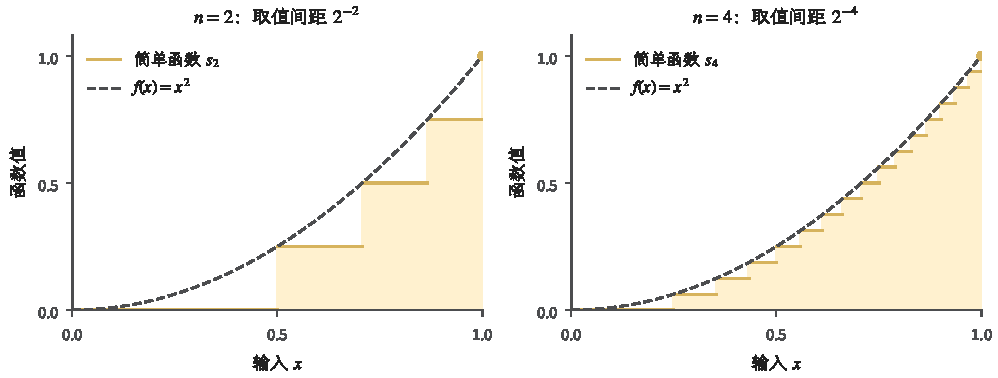
\includegraphics[width=\linewidth]{figures/01-mathematical-preliminaries/01-mathematical-language-combinatorics-analysis-optimization/matplotlib/concepts-analysis-functional/simple-integral.pdf}
 \caption{按取值分层的简单函数逼近。两图都使用式~\eqref{eq:analysis-canonical-simple-approximation}的构造，分别取$n=2$和$n=4$；本例中高度截断不起作用。黄色阶梯下的面积是有限加权和，目标曲线下的面积为$1/3$。两图共用坐标尺度。}
 \label{fig:analysis-simple-integral}
\end{figure*}
\begin{definition}[非负函数的Lebesgue积分]
\label{def:analysis-nonnegative-lebesgue-integral}
在测度空间$(X,\mathcal{A},\mu)$上，非负可测函数$f:X\to[0,\infty]$的积分定义为
\begin{equation}
  \int_X f\,\mathrm{d}\mu
  =
  \sup\left\{
    \int_X s\,\mathrm{d}\mu:
    0\leq s\leq f,\ s\text{为简单函数}
  \right\}.
\label{eq:analysis-nonnegative-lebesgue-integral}
\end{equation}
这里允许结果为$+\infty$。
\end{definition}
这个定义不要求把定义域切成连续小区间，而是按函数值分层，所以能自然处理极限和
零测例外。式~\eqref{eq:analysis-canonical-simple-approximation}给出的阶梯也可用来
计算这个上确界；下面的单调收敛定理说明，任意这样的递增逼近都能计算这个上确界。

\subsubsection{单调逼近与积分性质}
非负积分定义直接保留大小关系：若$0\leq f\leq g$，每个不超过$f$的简单函数
也不超过$g$，所以$\int f\,\mathrm d\mu\leq\int g\,\mathrm d\mu$。
它也继承零测修改不变性。设$N$可测且$\mu(N)=0$，$f,g$可测非负并在$X\setminus N$
相等。任取简单函数$0\leq s\leq f$，去掉$N$上的部分得到
$s\mathbb I_{X\setminus N}\leq g$，且简单函数积分没有改变；取上确界得到
$\int f\leq\int g$，反向同理。这里没有用一般积分的线性，只用了简单函数的有限和。
修改后的函数仍须可测；在未完备测度空间中，不能在零测集上任意修改而省略这项要求。

一种防止总量在逼近中消失的方式，是只让非负贡献逐步增加。它正好对应上面的下方阶梯。记$f_n(x)\uparrow f(x)$表示每个固定$x$处的数列单调增加且趋于$f(x)$；允许忽略零测例外时，例外须包含在同一个可测零测集中。下面把阶梯逼近推广到任意递增的非负可测函数列\scite{math-folland1999real}
\begin{theorem}[单调收敛定理]
\label{thm:analysis-monotone-convergence}
设$f_n,f:X\to[0,\infty]$可测，且$f_n(x)\uparrow f(x)$几乎处处，则
\[   \lim_{n\to\infty}\int_X f_n\,\mathrm{d}\mu   =   \int_X f\,\mathrm{d}\mu. \]
两边都允许取$+\infty$。
\end{theorem}
\begin{proof}
把单调性或收敛关系失效的可测零测集并为$N$，并将$f_n$与$f$在$N$上都改为$0$。
修改后的函数仍可测且积分不变，所以可假定$f_n\uparrow f$逐点成立。由
$0\leq f_n\leq f$，积分序列单调不减且
\[   L:=\lim_{n\to\infty}\int f_n\,\mathrm{d}\mu   \leq\int f\,\mathrm{d}\mu. \]
还需证明反向不等式。任取满足$0\leq s\leq f$的简单函数，将它写为 $s=\sum_{j=1}^m a_j\mathbb{I}_{E_j}$，其中$a_j>0$且$E_j$两两不交。固定 $c\in(0,1)$，定义
\[   E_{j,n}   =   E_j\cap\{x:f_n(x)\geq ca_j\}. \]
由于$f_n\uparrow f$且$f\geq a_j$于$E_j$，有$E_{j,n}\uparrow E_j$。
第~\ref{sec:analysis-set-measure-continuity}节已由可数可加性证明测度对递增集合连续，
故$\mu(E_{j,n})\uparrow\mu(E_j)$。同时
\[   f_n   \geq   c\sum_{j=1}^m a_j\mathbb{I}_{E_{j,n}}, \]
从而
\[   L   \geq   \lim_{n\to\infty}   c\sum_{j=1}^m a_j\mu(E_{j,n})   =   c\int s\,\mathrm{d}\mu. \]
先令$c\uparrow1$，再对所有$0\leq s\leq f$的简单函数取上确界。根据非负积分的定义~\eqref{eq:analysis-nonnegative-lebesgue-integral}， $L\geq\int f\,\mathrm{d}\mu$。与前一不等式合并即得结论。
\end{proof}

非负性避免正负无穷相消，单调性则保证已经积累的质量不会在后续消失。定理不要求存在一个可积的统一上界，也不要求各$\int f_n$有限。

单调收敛已经说明递增逼近怎样保留总量。积分还应继承有限和的两个基本规律：贡献增加时总量不能减少，非负线性组合的总量
等于各总量的同一线性组合。下面给出它们在一般测度空间中的版本；证明的任务是把
有限和的性质传到定义中的上确界，不能仅凭熟悉的Riemann积分规则就跳过这一推广。
\begin{lemma}[非负积分的线性与单调性]
\label{lem:analysis-nonnegative-integral-properties}
设$f,g:X\to[0,\infty]$可测，$\alpha,\beta\geq0$。若$f\leq g$几乎处处，则
\[
  \int_X f\,\mathrm{d}\mu\leq\int_X g\,\mathrm{d}\mu.
\]
此外，在$0\cdot\infty=0$的约定下，
\[
  \int_X(\alpha f+\beta g)\,\mathrm{d}\mu
  =
  \alpha\int_X f\,\mathrm{d}\mu
  +
  \beta\int_X g\,\mathrm{d}\mu.
\]
\end{lemma}
\begin{proof}
对$f\leq g$几乎处处的情形，集合$N=\{x:f(x)>g(x)\}$可测且$\mu(N)=0$。把$f$在
$N$上改为$0$得到可测函数$\widetilde f$，其积分与$f$相同，并且逐点满足
$\widetilde f\leq g$。此时每个满足$0\leq s\leq\widetilde f$的简单函数也满足
$s\leq g$；
在式~\eqref{eq:analysis-nonnegative-lebesgue-integral}中取上确界便得到单调性。

还需把简单函数的线性提升到一般非负函数。前面的单调收敛定理
\ref{thm:analysis-monotone-convergence}已保证：非负可测函数递增逼近其极限时，
积分也递增趋于极限的积分。现在分别取
非负简单函数$s_n\uparrow f$和$t_n\uparrow g$，则
$\alpha s_n+\beta t_n\uparrow\alpha f+\beta g$。对这三个函数列应用单调收敛定理，
结合简单函数的线性性，即得
\[
  \int_X(\alpha f+\beta g)\,\mathrm{d}\mu
  =
  \lim_{n\to\infty}
  \left(
    \alpha\int_Xs_n\,\mathrm{d}\mu
    +
    \beta\int_Xt_n\,\mathrm{d}\mu
  \right),
\]
右侧正是结论中的两个积分之和。
\end{proof}

简单函数的共同细分在单调收敛之前建立，一般函数的线性则在单调收敛之后建立；
两者不能倒置。对任意可测非负函数列$u_k$，再把线性用于有限部分和并用单调收敛，
还得到$\int\sum_{k\geq1}u_k=\sum_{k\geq1}\int u_k$，允许两边为无穷。
例如$(0,\infty)$上的$\mathbb I_{(0,n)}\uparrow1$，积分从$n$增至无穷；
单调收敛并不承诺最终总量有限。

\subsubsection{有符号积分与可积性}

非负函数只累积贡献，允许总量为$+\infty$。含正负值的函数却可能一边累积
$+\infty$、另一边累积$-\infty$，不能用二者相消来定义一个数。因此先把正、负贡献
分别计算，再决定它们是否允许相减。
\begin{definition}[有符号积分与可积性]
\label{def:analysis-integrable-function}
在测度空间$(X,\mathcal{A},\mu)$上，对可测实函数$f$，令
\[   f^+(x)=\max\{f(x),0\},\qquad   f^-(x)=\max\{-f(x),0\}. \]
若$\int_X f^+\,\mathrm{d}\mu$与$\int_X f^-\,\mathrm{d}\mu$不同时为无穷，则定义
\[
  \int_X f\,\mathrm{d}\mu
  =\int_X f^+\,\mathrm{d}\mu-\int_X f^-\,\mathrm{d}\mu.
\]
若
\begin{equation}
  \int_X|f|\,\mathrm{d}\mu<\infty,
\label{eq:analysis-absolute-integrability}
\end{equation}
就称$f$\term{绝对可积}（absolutely integrable）或Lebesgue可积。
\end{definition}
由于$f=f^+-f^-$且$|f|=f^++f^-$，可积性等价于正负两部分的积分都有限。
此时积分没有“无穷减无穷”的歧义，并满足
\[   \left|\int_X f\,\mathrm{d}\mu\right|   \leq   \int_X|f|\,\mathrm{d}\mu. \]

有符号线性也需要这项有限性。若$f,g$可积，$|f+g|\leq|f|+|g|$
先保证$f+g$可积。记$u=f+g$，由逐点恒等式
$u^++f^-+g^-=u^-+f^++g^+$，对两边的非负项积分并使用已证明的线性，
再移去有限项，得到$\int(f+g)=\int f+\int g$。
非负常数倍由前面的引理处理，负常数倍则交换正负部分，所以
$\int(\alpha f+\beta g)=\alpha\int f+\beta\int g$对任意实数$\alpha,\beta$成立。
若$f\leq g$几乎处处，对非负函数$g-f$积分还得到$\int f\leq\int g$。

在闭区间上有界且Riemann可积的函数也Lebesgue可积，两种积分取值相同。Lebesgue积分
并非否定熟悉的面积解释，而是扩大可处理的函数，并让两个可测且几乎处处相等的函数
具有相同积分。例如在Lebesgue测度下，修改可测函数在单点上的值仍得到可测函数，也不
改变积分。反过来，积分有限不表示函数处处有界，也不自动给出连续性。
例如在$(0,1)$上，$x^{-1/2}$无界却可积：对
$x^{-1/2}\mathbb I_{[1/n,1)}$用闭区间上的熟悉积分，再用单调收敛，得到
$\int_0^1x^{-1/2}\,\mathrm dx=\lim_n2(1-n^{-1/2})=2$。
而对$x^{-1}$同样计算得到$\lim_n\log n=+\infty$；它的非负积分有定义，
却不是可积函数。若在$(-1,1)$取$f(x)=1/x$（原点取$0$），正负部分积分都为无穷，
Lebesgue积分便没有定义。对称截断得到的零是另一种极限约定，不能替代这里的积分。

有限集合上的积分就是带测度权重的求和。回到第~\ref{sec:analysis-set-structures}节的$X=\{a,b\}$，
$\mu(\{a\})=1$、$\mu(\{b\})=2$，并令$f(a)=3$、$f(b)=-1$。则
\[
 \int_Xf\,\mathrm d\mu=3\times1+(-1)\times2=1,
 \qquad \int_X|f|\,\mathrm d\mu=5.
\]
积分是总量；若要把它称为平均，还要除以总质量$\mu(X)=3$，得到$1/3$。
概率测度的总质量为$1$，才无需这一步归一化。这个小例子也显示，正负部分可以相消，
可积性却要分别控制它们的大小。
一般地，按$\mu$取一个有限平均要求$f$可积且$0<\mu(X)<\infty$，此时平均为
$\mu(X)^{-1}\int_X f\,\mathrm d\mu$。总质量为零时不能相除，总质量无穷时也不能把
有限积分除以无穷来定义这项平均；需要另行指定局部区域或归一化方式。

\subsection{乘积积分与次序交换}

前面讨论的是一个位置$x$上的贡献；若函数同时依赖$x$和$y$，就要给成对位置
$(x,y)$所在的集合赋权重。对两组分别给定的权重，最自然的扩展是让矩形
$A\times B$的权重等于两边权重的乘积。它是面积“长乘宽”以及有限双重加权和的
共同推广，称为乘积测度。

为了由矩形权重唯一确定一般集合的权重，下面采用一种常见条件：整个空间可以由
可数个有限权重的区域覆盖。这比要求空间的总权重有限宽松，例如整个实数轴长度无限，
却能写成区间$[-n,n]$的并。
\begin{definition}[$\sigma$有限测度]
\label{def:analysis-sigma-finite-measure}
若存在$E_n\in\mathcal{A}$，使$X=\bigcup_{n=1}^{\infty}E_n$且对每个$n$有
$\mu(E_n)<\infty$，称测度空间$(X,\mathcal{A},\mu)$是
\term{$\sigma$有限}（sigma-finite）的。
\end{definition}
例如$\mathbb N$上的计数测度可由有限集合$\{1,\ldots,n\}$覆盖，因而$\sigma$有限；
不可数集合上的计数测度则不满足这一条件，因为可数个有限集合的并仍然可数。
所以“每个点质量有限”远弱于“整个空间能由可数个有限质量区域覆盖”。

在两个$\sigma$有限测度空间上，乘积测度定理保证：矩形上的乘积权重能扩展为一个
存在且唯一的测度。下面用这一性质刻画它。
\begin{definition}[乘积$\sigma$代数与乘积测度]
\label{def:analysis-product-measure}
给定两个$\sigma$有限测度空间$(X,\mathcal{A},\mu)$与$(Y,\mathcal{B},\nu)$。
包含所有矩形$A\times B$（$A\in\mathcal{A}$，$B\in\mathcal{B}$）的最小
$\sigma$代数称为乘积$\sigma$代数，记为$\mathcal{A}\otimes\mathcal{B}$。
在该$\sigma$代数上，对任意这样的$A,B$满足
\[   (\mu\otimes\nu)(A\times B)=\mu(A)\nu(B) \]
的测度记为$\mu\otimes\nu$，称为\term{乘积测度}（product measure）。
这里仍约定$0\cdot\infty=0$。
\end{definition}
对矩形上的指示函数，先对$x$积分或先对$y$积分都得到同一个乘积。一般函数能否继续交换积分次序，则取决于非负性或绝对可积性，下面给出准确条件。若脱离$\sigma$有限框架，乘积测度的唯一性和相应积分结论需要
更谨慎的版本。

有限网格把这个构造还原为双重求和。若$X=\{x_1,\ldots,x_m\}$、
$Y=\{y_1,\ldots,y_n\}$分别带权重$u_i,v_j$，则
\[
  \int_{X\times Y}f\,\mathrm{d}(\mu\otimes\nu)
  =
  \sum_{i=1}^m\sum_{j=1}^n f(x_i,y_j)u_iv_j.
\]
有限和可以直接交换次序；一般测度空间中的累次积分还要处理无穷值与极限，
不能只由矩形公式推出。还要注意，乘积测度是一种特定构造；一般的二元概率分布
可以包含两个变量之间的依赖，并不必然等于两边概率测度的乘积。第~\ref{chap:probability-theory}章会
在联合分布与独立性的语境中回用这一区别。

乘积测度确定成对位置的权重，尚未保证任意函数都能按两个次序分别累计。这里比较累次积分与乘积空间上的积分：非负性允许逐步累计，绝对可积性排除正负无穷相消；刚建立的单调收敛把简单函数的累计规则推广到一般非负函数。
\begin{theorem}[Tonelli与Fubini定理]
\label{thm:analysis-tonelli-fubini}
设$(X,\mathcal{A},\mu)$与$(Y,\mathcal{B},\nu)$为$\sigma$有限测度空间，且 $f:X\times Y\to\overline{\mathbb{R}}$对乘积$\sigma$代数可测。
\begin{itemize}

\item 若$f\geq0$，则每个截面$y\mapsto f(x,y)$与$x\mapsto f(x,y)$都可测，并且两个
  内层积分函数
  \[
    x\longmapsto\int_Yf(x,y)\,\mathrm{d}\nu(y),
    \qquad
    y\longmapsto\int_Xf(x,y)\,\mathrm{d}\mu(x)
  \]
  分别关于$x$与$y$可测，且
  \[
    \begin{aligned}
      \int_{X\times Y}f\,\mathrm{d}(\mu\otimes\nu)
      &=
      \int_X\left(\int_Yf(x,y)\,\mathrm{d}\nu(y)\right)\mathrm{d}\mu(x)\\
      &=
      \int_Y\left(\int_Xf(x,y)\,\mathrm{d}\mu(x)\right)\mathrm{d}\nu(y).
    \end{aligned}
  \]
  允许共同值为$+\infty$。这是Tonelli定理。
\item 若$\int_{X\times Y}|f|\,\mathrm{d}(\mu\otimes\nu)<\infty$，则
  $y\mapsto f(x,y)$对几乎每个$x$可积，$x\mapsto f(x,y)$对几乎每个$y$可积。
  把相应内层积分函数在例外集上置为$0$后，它们分别可积，上述等式对$f$成立并取有限值。
  这是Fubini定理。
\end{itemize}
\end{theorem}

证明可分为集合与函数两层。对矩形指示函数$\mathbb I_{A\times B}$，三种积分都等于
$\mu(A)\nu(B)$；有限可加性把这个结论扩展到有限分割形成的集合。
从这些集合进入乘积$\sigma$代数中的\emph{任意}可测集合，还需要测度论的扩张论证，
不是仅靠每个矩形上的等式便能完成；完整论证见所引测度论教材
\scite{math-folland1999real}
本章关注扩张之后的函数层：指示函数的结论经线性组合进入非负简单函数，再经
$s_n\uparrow f$和单调收敛进入任意非负可测函数，得到Tonelli。
若$f$绝对可积，则对$f^+$和$f^-$分别应用Tonelli；绝对积分有限保证两部分不会
出现无穷减无穷，相减才得到Fubini。这里给出证明的依赖路线，不把矩形核对当作
完整证明。

这里非负性允许无穷值，绝对可积性则排除了依赖积分次序的条件相消。例如在
$\mathbb{N}\times\mathbb{N}$上使用计数测度时，Tonelli说明非负双重级数可以任意交换
求和次序；Fubini说明绝对收敛的双重级数也可以这样做。若既不非负也不绝对可积，
交换次序可能改变结果，甚至一个次序收敛而另一个发散。因此“把两个积分换一下”
不是排版操作，而是需要先核对函数符号或绝对积分的数学步骤。

\begin{example}[行列各自可加仍不足以换序]
\label{ex:analysis-iterated-sum-failure}
在$\mathbb N\times\mathbb N$上令
$a_{i,j}=\mathbb I\{j=i\}-\mathbb I\{j=i+1\}$，两边均用计数测度。
每一行只有一个$1$和一个$-1$，故$\sum_j a_{i,j}=0$；
第一列的和为$1$，其余每一列的和为$0$。于是
\[
 \sum_{i=1}^{\infty}\left(\sum_{j=1}^{\infty}a_{i,j}\right)=0,
 \qquad
 \sum_{j=1}^{\infty}\left(\sum_{i=1}^{\infty}a_{i,j}\right)=1.
\]
两种累次和都有有限值，却不相等。每行的绝对值和为$2$，所以整个绝对积分为无穷，
正负部分也各为无穷。失效的是Fubini的绝对可积条件，而非某一行的计算规则。
\end{example}

$\sigma$有限也有实际作用。在$[0,1]$上让$x$采用Lebesgue测度、$y$采用
不可数集合上的计数测度，取非负函数$f(x,y)=\mathbb I\{x=y\}$。
对角线属于乘积$\sigma$代数，但先对$y$计数再对$x$积分得到$1$，
先对$x$求长度再对$y$计数却得到$0$。这里不满足本章Tonelli版本的$\sigma$有限条件，
不能只凭非负性换序。

\subsection{积分换元与坐标变换}
\label{sec:analysis-coordinate-change-integral-applications}
积分的定义、权重和可积条件已经确定，现在可以利用函数或区域的结构计算它。
换元重新表示同一个区域，函数值要随坐标复合，每块区域的体积权重也要随之修正。
链式法则中的Jacobian把一个输入扰动映成输出扰动；这里则需要把多个方向共同张成的
体积缩放成一个非负权重，起作用的是Jacobian行列式的绝对值。

一维换元中，$u=T(x)$把长度$\mathrm{d}x$缩放为约 $|T'(x)|\mathrm{d}x$。在$d$维，局部线性近似
\[   T(\bm{x}+\bm{h})   \approx   T(\bm{x})+\bm{J}_T(\bm{x})\bm{h} \]
把一个小平行多面体的有向体积乘以 $\det\bm{J}_T(\bm{x})$，普通体积则乘以其绝对值。行列式为零意味着至少一个方向被压扁，局部逆映射通常不再存在。

设$U,V\subseteq\mathbb{R}^d$为开集， $T:U\to V$是连续可微双射，逆映射也连续可微，并且 $\det\bm{J}_T(\bm{x})\neq0$。对非负可测函数或绝对可积函数$g$，多维换元公式为
\begin{equation}
  \int_V g(\bm{y})\,\mathrm{d}\bm{y}
  =
  \int_U
  g\bigl(T(\bm{x})\bigr)
  \left|\det\bm{J}_T(\bm{x})\right|
  \,\mathrm{d}\bm{x}.
\label{eq:analysis-multivariate-change-variables}
\end{equation}
绝对值不可省略，因为积分中的体积不随坐标方向翻转而变成负数。一维单调换元是 $d=1$的特例；若在定积分中保留有向上下限，也可让导数符号由上下限次序吸收。
公式的证明可理解为把$U$分成足够小的区域：在每一块上用
$T(\bm{x}+\bm{h})\approx T(\bm{x})+\bm{J}_T(\bm{x})\bm{h}$替代原映射，
线性映射把该块体积乘以$|\det\bm{J}_T(\bm{x})|$，再让分割尺度趋于零。
这条路线只提供直观框架；严格证明还要控制局部近似误差、像集重叠和可测逼近，
不能把逐点线性化直接当作全局换元等式。
\begin{example}[极坐标中的面积权重]
\label{ex:analysis-polar-coordinate-jacobian}
令$D=\{\bm{x}\in\mathbb{R}^2:\lVert\bm{x}\rVert_2\leq1\}$，并令
$T(r,\theta)=(r\cos\theta,r\sin\theta)$。在开集
$(0,1)\times(0,2\pi)$上，$T$是到开圆盘内部去掉原点和正$x$轴径向接缝后的区域的
连续可微双射，逆映射也连续可微。其Jacobian矩阵的行列式为
\[   \det
\begin{bmatrix}     \cos\theta & -r\sin\theta\\     \sin\theta & r\cos\theta
\end{bmatrix}   =r. \]
圆周、原点和径向接缝都是二维零测集；参数矩形的边界也是零测集。因此在上述开集上应用
换元公式，再补回这些零测部分，便得到
\[   \int_D1\,\mathrm{d}\bm{x}   =   \int_0^{2\pi}\int_0^1r\,\mathrm{d}r\,\mathrm{d}\theta   =\pi. \]
这里积分上下限包含端点不改变积分值。若参数化在正测度区域上重复覆盖，则不能直接使用
上述双射版本，否则同一点会被重复计数。
\end{example}
\subsection{微分与积分的关系}

换元改变坐标表示，以下公式则把局部变化的累计与端点或边界联系起来。
一维乘积求导产生分部积分，沿曲线的链式求导产生端点差，区域中的流出率则对应边界通量。
三种关系采用不同的积分对象，不能省去各自的端点、方向或面积权重。

\subsubsection{分部积分与积分余项}
\label{sec:analysis-integration-remainders}

先回顾微积分基本定理的连续版本。若$g$在$[a,b]$上连续，
$H(x)=\int_a^xg(t)\,\mathrm dt$在内点处满足$H'(x)=g(x)$；
若$H\in C^1([a,b])$，则$\int_a^bH'(x)\,\mathrm dx=H(b)-H(a)$。
这里$C^1$表示一阶连续可微，在闭区间端点采用单侧导数的连续延拓。
第一条可由
$[H(x+h)-H(x)]/h-g(x)=h^{-1}\int_x^{x+h}(g(t)-g(x))\,\mathrm dt$
和连续性得到；第二条再对$H(x)-H(a)-\int_a^xH'(t)\,\mathrm dt$
使用零导数蕴含常值的中值定理。这说明所用的是连续导数的积分，不是
“几乎处处存在导数便能恢复函数”的无条件结论。

有些乘积的积分难算，但把导数转移到另一个因子后会简化。分部积分就是这种转移规则，代价是增加边界贡献。若$u,v\in C^1([a,b])$，由乘积求导$(uv)'=u'v+uv'$并在$[a,b]$上积分，可得
\begin{equation}
  \int_a^b u(x)v'(x)\,\mathrm{d}x
  =
  [u(x)v(x)]_a^b
  -
  \int_a^b u'(x)v(x)\,\mathrm{d}x.
\label{eq:analysis-integration-by-parts}
\end{equation}
例如，取$u(x)=x$、$v'(x)=e^x$，得到 $\int_0^1xe^x\,\mathrm{d}x=[xe^x]_0^1-\int_0^1e^x\,\mathrm{d}x=1$。边界项不能无故删除；只有在函数于边界消失、区域无边界，或衰减速度足以使无穷远边界项趋零时才能省略。

分部积分还能把第~\ref{sec:analysis-taylor-approximation}节的局部二阶变化累计成有限位移的
余项。设连接$\bm{x}$与$\bm{x}+\bm{h}$的线段包含在一个开集内，且$f$在该开集上二阶
连续可微。令$\phi(t)=f(\bm{x}+t\bm{h})$，对$(1-t)\phi''(t)$在$[0,1]$上分部积分，得到
\[
  \int_0^1(1-t)\phi''(t)\,\mathrm{d}t
  =-\phi'(0)+\phi(1)-\phi(0).
\]
用链式法则代回，便得到不挑选中间点的Taylor积分余项：
\[   f(\bm{x}+\bm{h})   =   f(\bm{x})   +\nabla f(\bm{x})^{\top}\bm{h}   +   \int_0^1(1-t)   \bm{h}^{\top}\nabla^2f(\bm{x}+t\bm{h})\bm{h}\,\mathrm{d}t. \]
权重$1-t$说明越靠近位移起点的曲率贡献被累计得越多；该表达式与前面的中间点余项
描述同一有限变化，但保留了整条线段上的曲率信息。

一般阶数也由同一操作得到。设$f$在连接$x_0$和$x_0+h$的线段邻域内
$r+1$阶连续可微，$r\geq0$，令$\phi(t)=f(x_0+th)$。
记
\[
 I_r=\frac1{r!}\int_0^1(1-t)^r\phi^{(r+1)}(t)\,\mathrm dt.
\]
基本定理给出$I_0=\phi(1)-\phi(0)$；对$r\geq1$分部积分，
\[
 I_r=-\frac{\phi^{(r)}(0)}{r!}
       +\frac1{(r-1)!}\int_0^1(1-t)^{r-1}\phi^{(r)}(t)\,\mathrm dt
     =-\frac{\phi^{(r)}(0)}{r!}+I_{r-1}.
\]
逐次代入并用$\phi^{(k)}(0)=h^k f^{(k)}(x_0)$，便得
\begin{equation}
 f(x_0+h)=\sum_{k=0}^r\frac{f^{(k)}(x_0)}{k!}h^k
 +\frac{h^{r+1}}{r!}
   \int_0^1(1-t)^r f^{(r+1)}(x_0+th)\,\mathrm dt.
\label{eq:analysis-taylor-integral-remainder}
\end{equation}
参数化$x_0+th$同时处理正、负$h$。若$|f^{(r+1)}|\leq M$，积分权重的总量为
$1/(r+1)$，故余项不超过$M|h|^{r+1}/(r+1)!$，与前面的中间点余项界一致。
例如立方函数在$r=2$时有$f'''=6$，余项就是
$(h^3/2)\int_0^1 6(1-t)^2\,\mathrm dt=h^3$。
多元函数沿$\phi(t)=f(\bm x+t\bm h)$使用同一公式；$r=1$便还原前述Hessian积分余项。

\subsubsection{路径积分与端点关系}

换元仍是在同维区域内计算体积积分；如果贡献只沿一条路径累积，就应改用弧长或带方向的路径增量，不能继续套用全空间体积权重。设分段连续可微路径$\gamma:[a,b]\to\mathbb{R}^d$。对沿路径连续的标量函数
$h:\mathbb{R}^d\to\mathbb{R}$，标量线积分定义为
\[
  \int_\gamma h\,\mathrm{d}s
  =
  \int_a^b h(\gamma(t))\lVert\gamma'(t)\rVert_2\,\mathrm{d}t.
\]
速度的范数把参数增量换成弧长，因此反转路径方向不改变该积分。对沿路径连续的向量场
$\bm{F}:\mathbb{R}^d\to\mathbb{R}^d$，向量场线积分则定义为
\[   \int_{\gamma}\bm{F}\mathbin{\cdot}\mathrm{d}\bm{r}   =   \int_a^b   \bm{F}(\gamma(t))^{\top}\gamma'(t)\,\mathrm{d}t. \]
若$\bm{F}=\nabla\phi$且$\phi$连续可微，链式法则给出
\begin{equation}
  \int_{\gamma}\nabla\phi\mathbin{\cdot}\mathrm{d}\bm{r}
  =
  \phi(\gamma(b))-\phi(\gamma(a)).
\label{eq:analysis-line-integral-gradient}
\end{equation}
因此梯度场的路径积分只依赖端点。向量场线积分在路径方向反转时变号；若漏掉参数化导数
$\gamma'(t)$，就会丢失方向和行进速度的信息。

\begin{example}[同一路径上的长度、端点差与环流]
\label{ex:analysis-path-integral-comparison}
取单位圆的上半圆路径$\gamma(t)=(\cos t,\sin t)$，$0\leq t\leq\pi$。
它的速度范数恒为$1$，所以$\int_\gamma1\,\mathrm ds=\pi$。
取$\phi(x,y)=x$，则$\nabla\phi=(1,0)^\top$，
\[
 \int_\gamma\nabla\phi\mathbin{\cdot}\mathrm d\bm r
 =\int_0^\pi-\sin t\,\mathrm dt=-2
 =\phi(-1,0)-\phi(1,0).
\]
换成旋转场$\bm F(x,y)=(-y,x)^\top$时，
$\bm F(\gamma(t))^\top\gamma'(t)=1$，沿上半圆的积分为$\pi$。
但沿同样端点的直径路径$\eta(t)=(1-2t,0)$，$0\leq t\leq1$，
内积恒为零，积分为$0$。向量场连续甚至光滑，也不能单独保证路径无关。
沿完整单位圆逆时针一周，这个旋转场的积分为$2\pi$；梯度场沿闭合路径的端点差
必须为零，所以它不可能在整个平面上写成一个连续可微势函数的梯度。
\end{example}

\subsubsection{散度积分与边界通量}
路径积分沿行进方向累计，通量则计算穿过边界的贡献。在向量场
$\bm F=(F_1,\ldots,F_d)^\top$中，散度定义为
$\nabla\mathbin{\cdot}\bm F=\sum_{i=1}^d\partial F_i/\partial x_i$；
它把各坐标方向的局部流出率相加。相邻小区域的公共边界法向相反，
内部交换在总和中相消，剩下的应是外边界的净流出。

以下采用经典的规则区域版本：$\Omega$是有界开区域，其边界由有限个$C^1$
曲面片组成，每个光滑片附近区域位于边界的一侧，片间接缝的边界面积为零。
光滑区域、多边形和通常的多面体均符合这一条件。若向量场$\bm{F}$
在$\overline{\Omega}$的一个开邻域内连续可微，
\term{散度定理}（divergence theorem）写成
\begin{equation}
  \int_{\Omega}\nabla\mathbin{\cdot}\bm{F}\,\mathrm{d}\bm{x}
  =
  \int_{\partial\Omega}\bm{F}^{\top}\bm{n}\,\mathrm{d}S,
\label{eq:analysis-divergence-theorem}
\end{equation}
其中$\bm{n}$是外单位法向量，$\mathrm dS$表示边界上的面积元素。这个公式把区域内部与区域边界两种积分联系起来；左边汇总区域内部的局部流出率，右边计算穿过边界的净通量。它的严格适用条件随区域与函数空间版本而异；带尖点、无界区域或弱导数时，需要使用相应推广并重新核对边界项。分部积分、路径积分与散度定理共同说明，局部导数进入整体积分时， 通常会留下不可忽略的边界信息。

例如单位开圆盘$\Omega$上的$\bm F(x,y)=(x,y)^\top$有散度$2$，
故左边为$2\pi$。边界参数化$\gamma(t)=(\cos t,\sin t)$，$0\leq t\leq2\pi$，
外单位法向就是$\bm n=\gamma(t)$，弧长元素为$\mathrm dS=\mathrm dt$；
因此$\bm F^\top\bm n=1$，右边也为$2\pi$。
改用内法向会得到$-2\pi$，这不是同一定理中的方向约定。
前例的旋转场散度为零，且在圆周上始终与法向垂直，所以通量为零，
尽管沿切向的环流为$2\pi$。这一区别说明线积分和通量计算的不是同一种贡献。

\section{函数列的收敛与性质保持}
\label{sec:analysis-function-convergence-essential-bounds}

现在让被研究的函数本身随索引变化。$f_n:X\to\mathbb R$仍是一个序列，只是每一项
是函数；固定$x$以后，$f_n(x)$才成为第~\ref{sec:analysis-sequences-series-errors}节
的数值序列。比较整个函数还要选择误差尺度，并判断极限是否保留连续性、变化率或积分。
这些任务所需的基础不同：逐点收敛只需要数值极限，一致误差使用上确界，几乎处处
回用零测集，积分误差回用积分，导数逼近则回用第~\ref{sec:analysis-local-models}节
建立的局部变化信息。

\subsection{收敛方式与极限存在}
\subsubsection{逐点收敛与一致收敛}

固定一个输入以后，比较的只是一列实数。这里不需要函数可微或可积，甚至不需要
在输入集合上指定距离；函数值仍按实数绝对值比较。
\begin{definition}[逐点收敛]
\label{def:analysis-pointwise-almost-everywhere-convergence}
设$f_n,f:X\to\mathbb{R}$。若
\[
 \begin{gathered}
  \forall x\in X,\quad
  \forall\varepsilon>0,\quad
  \exists N=N(x,\varepsilon)\in\mathbb N,\\
  \forall n\geq N,\quad
  |f_n(x)-f(x)|<\varepsilon,
 \end{gathered}
\]
即对每个$x$都有$\lim_n f_n(x)=f(x)$，称$f_n$逐点收敛到$f$。
\end{definition}


定义中的每个位置都只比较一列实数；整体误差却不能靠分别检查各位置来控制。
即使每个输入处的误差最终都很小，开始稳定的时刻仍可能依赖输入。
若希望一次选定迭代次数后就控制全部输入，需要更强的一致条件。
\begin{definition}[函数列的一致收敛]
\label{def:analysis-uniform-convergence}
设$X$为非空集合，$f_n,f:X\to\mathbb R$。若
\[
  \forall\varepsilon>0,\quad
  \exists N=N(\varepsilon)\in\mathbb N,\quad
  \forall x\in X,\quad
  \forall n\geq N,\quad
  |f_n(x)-f(x)|<\varepsilon,
\]
就称$f_n$在$X$上一致收敛到$f$。等价地，
\begin{equation}
  \lVert f_n-f\rVert_{\infty}
  :=
  \sup_{x\in X}|f_n(x)-f(x)|
  \longrightarrow0.
\label{eq:analysis-uniform-convergence}
\end{equation}
这里的上确界检查全部输入，没有忽略零测集。
\end{definition}


两条定义的区别落在量词次序。逐点收敛允许$N$依赖$x$；一致收敛把$\exists N$
移到$\forall x$之前，同一个$N$必须同时控制全部输入。区别不在“趋近”这个词，
而在误差阈值之后允许谁依赖谁。下面用同一列函数比较这两种控制。

在$[0,1]$上取$f_n(x)=x^n$。它逐点收敛到
\[
 f(x)=
 \begin{cases}
  0,&0\leq x<1,\\
  1,&x=1.
 \end{cases}
\]
每个固定的$0<x<1$都有$x^n\to0$，而端点$1$的值始终为$1$。
但对每个$n$，$\sup_{0\leq x<1}x^n=1$，所以收敛不一致。
从量词看，固定$\varepsilon=1/2$后，无论选多大的$N$，在$n=N$时
总能选$x_N=(3/4)^{1/N}<1$，使误差$x_N^N=3/4>\varepsilon$。
失败的位置可以随$n$移动；不能把“每个位置最终变小”改写成“某一轮以后所有位置都小”。
若把范围缩为$[0,a]$，其中$a<1$，则上确界误差为$a^n\to0$，同一公式又变成一致收敛。

\subsubsection{几乎处处收敛与积分误差}

如果某些输入占零权重，是否必须在它们上面也逼近？积分任务通常不需要，
但必须先固定采用的测度和可忽略的范围。
\begin{definition}[几乎处处收敛]
\label{def:analysis-almost-everywhere-convergence}
给定测度空间$(X,\mathcal A,\mu)$和实函数$f_n,f$，若存在$E\in\mathcal A$、
$\mu(E)=0$，使
\[
 \forall x\in X\setminus E,\quad
 \forall\varepsilon>0,\quad
 \exists N=N(x,\varepsilon),\quad
 \forall n\geq N,\quad |f_n(x)-f(x)|<\varepsilon,
\]
就称$f_n$在$\mu$下几乎处处收敛到$f$。
\end{definition}
这里是先选一个零测集，再在它的补集上逐点收敛；每个精度和每一项不能任意丢掉
不同的正测度区域。可数个零测例外可以取并后统一，任意不可数个零测集的并却未必零测。
例如$x^n$关于$[0,1]$上的Lebesgue测度几乎处处趋于零，虽然它不在$x=1$处趋于零。
又如$f_n(x)=n\mathbb I_{\{0\}}(x)$几乎处处趋于零，但在$0$处连有限极限都没有。
若要求极限仍可测，本章采用各$f_n,f$均可测的版本；在未完备空间中，
不能从几乎处处关系自动推出任意指定的例外点取值可测。

如果关心的是按测度累计的误差，就要先说明被比较的函数属于什么空间。
积分不区分只在零测集上不同的可测函数：即使$f$不处处为零，$\int|f|^p\,\mathrm d\mu$
也可能为零。把这类函数视为同一个元素，才能让零误差对应空间中的同一个对象。
\Needspace{12\baselineskip}
\begin{definition}[$L^p$空间与范数]
\label{def:analysis-lp-space}
设$(X,\mathcal A,\mu)$为测度空间，$1\leq p<\infty$。对可测实函数定义等价关系
\[
  f\sim g\quad\Longleftrightarrow\quad f=g\text{在$\mu$下几乎处处成立}.
\]
$L^p(\mu)$由满足$\int_X|f|^p\,\mathrm d\mu<\infty$的可测实函数的等价类$[f]$组成，
其范数定义为
\[
  \lVert[f]\rVert_{L^p(\mu)}
  =\left(\int_X|f|^p\,\mathrm d\mu\right)^{1/p}.
\]
该值不依赖代表元的选择。下文用代表元$f$代写等价类$[f]$，并简记范数为
$\lVert f\rVert_p$。
\end{definition}

固定这个空间以后，函数列的收敛就可以由累计误差定义。
\begin{definition}[$L^p$收敛]
\label{def:analysis-lp-convergence}
设$1\leq p<\infty$，且$f_n,f\in L^p(\mu)$。若
\begin{equation}
  \lVert f_n-f\rVert_p
  :=
  \left(
    \int_X|f_n-f|^p\,\mathrm{d}\mu
  \right)^{1/p}
  \longrightarrow0,
  \qquad 1\leq p<\infty.
\label{eq:analysis-lp-convergence}
\end{equation}
就称$f_n$在$L^p(\mu)$中收敛到$f$。
\end{definition}
展开量词就是：对每个$\varepsilon>0$存在$N$，使所有$n\geq N$的
积分误差范数小于$\varepsilon$。这里受控的是整个积分，不是对每个$x$
分别要求$|f_n(x)-f(x)|<\varepsilon$。

回到上面的$f_n(x)=x^n$及其逐点极限$f$，对任意有限$p\geq1$，
\[   \lVert f_n-f\rVert_p^p   =   \int_0^1x^{np}\,\mathrm{d}x   =   \frac{1}{np+1}   \longrightarrow0. \]
同一函数列因此逐点且在每个有限$L^p$意义下收敛，却不一致收敛。区别来自最坏输入与累计误差采用了不同尺度。
图~\ref{fig:analysis-power-convergence-scales}把接近$x=1$的区域与误差数值并列。
每个固定的$x<1$最终都会下降，但每一轮总有更靠近$1$的新位置保留接近$1$的误差。
\begin{figure*}[htbp]
 \centering
 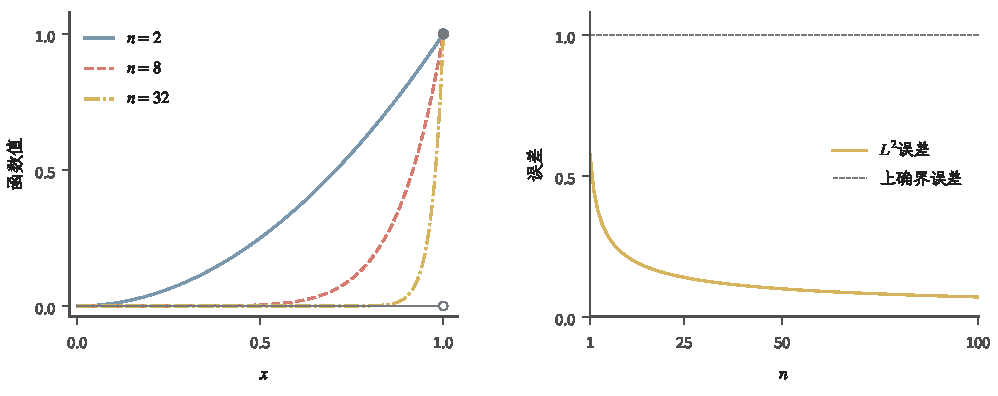
\includegraphics[width=\linewidth]{figures/01-mathematical-preliminaries/01-mathematical-language-combinatorics-analysis-optimization/matplotlib/teaching-analysis/analysis-power-convergence-scales.pdf}
 \caption{$x^n$在$[0,1]$上的两种整体尺度。左图蓝、红、黄线分别取$n=2,8,32$；灰线与端点标记表示逐点极限，
 它在$x<1$处为零、在$x=1$处为$1$。右图黄色曲线为精确的$L^2$误差$(2n+1)^{-1/2}$，
 灰虚线为始终等于$1$的普通上确界误差；单点$x=1$的修改不影响积分。图为解析教学示例。}
 \label{fig:analysis-power-convergence-scales}
\end{figure*}


若$\mu(X)<\infty$且$f_n,f\in L^p$，一致收敛蕴含$L^p$收敛，因为
\[   \lVert f_n-f\rVert_p   \leq   \mu(X)^{1/p}\lVert f_n-f\rVert_{\infty}. \]
当空间测度无穷时，即使各项仍属于$L^p$，这个推论也可能失败。在$\mathbb R$上采用
Lebesgue测度，固定$1\leq p<\infty$，并取
\[
  f_n(x)=\frac1n\mathbb I_{[0,n^p]}(x).
\]
每个$f_n$都属于$L^p$，且$\sup_x|f_n(x)|=1/n\to0$，所以一致收敛到零；但
\[
  \lVert f_n\rVert_p^p=\frac{n^p}{n^p}=1,
\]
因而不在$L^p$中收敛到零。幅度虽降低，非零区域却同步扩大，累计误差没有随之减小。

反过来，积分误差小也不保证整列在几乎每个点收敛。
\begin{example}[小区间轮流扫过定义域]
\label{ex:analysis-lp-without-ae-limit}
在$[0,1)$上按轮次细分区间，令
\[
 f_{2^k+j}(x)=\mathbb I_{[j2^{-k},(j+1)2^{-k})}(x),
 \qquad k=0,1,\ldots,\quad j=0,\ldots,2^k-1.
\]
第$k$轮依次访问$2^k$个小区间，每个函数的$L^p$范数为$2^{-k/p}$，
所以对每个有限$p\geq1$，$f_n\to0$在$L^p$中成立。
但每个$x\in[0,1)$在每轮恰有一次取值$1$，也在无穷多个其他时刻取值$0$。
因此整列在每个$x$处都不收敛。积分看到每次被访问的区间越来越小，
逐点收敛却要求同一个输入从某一时刻起一直稳定，这两个要求不能互代。
\end{example}

普通上确界会被单个异常点改变，而保持可测性的零测集修改不影响积分。
若仍要控制最坏误差，却允许忽略测度为零的例外，就应比较函数绝对值的本质上界。
\begin{definition}[本质有界与绝对值的本质上界]
\label{def:analysis-essential-bound}
设$(X,\mathcal A,\mu)$为测度空间，$f:X\to\mathbb R$可测。其绝对值$|f|$的
\term{本质上确界}（essential supremum）定义为
\[   \operatorname*{ess\,sup}_{x\in X}|f(x)|   =   \inf\{M\geq0:|f(x)|\leq M\text{几乎处处}\}. \]
若集合中没有有限的$M$，上式取$+\infty$；若上式有限，就称$f$本质有界。
这里衡量的是$|f|$的大小，不是一般有符号函数$f$的本质上确界。
\end{definition}

\begin{definition}[$L^\infty$空间与范数]
\label{def:analysis-linfty-space}
在同一测度空间上，$L^\infty(\mu)$由本质有界可测实函数的几乎处处等价类组成，
其范数定义为
\begin{equation}
  \lVert f\rVert_{L^\infty}
  =
  \operatorname*{ess\,sup}_{x\in X}|f(x)|.
\label{eq:analysis-essential-supremum-norm}
\end{equation}
同样用$f$代写等价类$[f]$；该范数不依赖代表元。
\end{definition}
例如在$[0,1]$上使用Lebesgue测度，令$f(0)=100$、其余位置$f(x)=0$，
则普通上确界为$100$，$|f|$的本质上确界却为$0$。
相应地，$\lVert f_n-f\rVert_{L^\infty}\to0$称为$L^\infty$收敛。
对每个$\varepsilon>0$，它要求某个$N$之后的全部误差都在几乎处处意义下
小于$\varepsilon$。可取精度$1/k$，把各$n,k$对应的可测零测例外并为一个零测集$E$；
于是存在同一个$E$，使$f_n$在$X\setminus E$上一致收敛。
反之，这种补集上的一致收敛立即给出$L^\infty$收敛。
因此它蕴含几乎处处收敛，却不一定是原集合上的一致收敛。
上面的$n\mathbb I_{\{0\}}$在$L^\infty$中恒等于零，普通上确界却为$n$。
对$x^n$，本质上确界误差仍为$1$，因为接近$1$的一整段正测度区间保留大误差，
不是删除端点就能消除。

$L^\infty$与有界函数上的普通上确界范数采用不同的对象：普通上确界范数区分
单点修改，$L^\infty$范数忽略的是$\mu$零测集上的修改。对$1\leq p<\infty$，
定义~\ref{def:analysis-lp-space}中的积分表达式满足齐次性和三角不等式，
而几乎处处等价关系保证范数为零时，空间中的元素就是零元素。
这里“范数”指非负、绝对齐次、满足三角不等式且只在零元素上为零的长度函数；
$L^p$的三角不等式及完整空间理论留到第~\ref{chap:functional-analysis-and-approximation}章。
当$0<p<1$时，同一积分表达式仍可用来度量误差大小，但通常不满足三角不等式，
所以不是范数；本章不把这一区间记作范数空间。

一个固定函数序列的一致收敛，讨论的是$n$增大时对所有输入能否共同控制。统计学习中“经验平均一致逼近总体平均”通常还要对候选函数类取上确界，控制对象形如
\[   \sup_{f\in\mathcal{F}}   \left|     \frac1n\sum_{i=1}^nf(X_i)-\int f\,\mathrm{d}P   \right|. \]
这里的一致性针对候选函数$f\in\mathcal{F}$，不是本节式~\eqref{eq:analysis-uniform-convergence}中针对输入$x\in X$的一致收敛。两者都出现上确界，却不能混为同一概念。
其中$X_1,\ldots,X_n$是来自分布$P$的样本，$\mathcal F$是待比较的可积函数类。
逐个$f$找到的样本量要求可以不同；对$\mathcal F$一致则要求一个共同的样本量控制整类函数。

几乎处处和$L^p$范数还依赖所选测度。若$Q$对$P$\term{绝对连续}
（absolutely continuous），记作$Q\ll P$，则原来$P$意义下的零测例外在$Q$下仍可忽略；
也就是对任意可测$A$，$P(A)=0$蕴含$Q(A)=0$。
这一测度关系不等同于前面映射的连续性；概率论中的正式展开见定义~\ref{def:probability-absolute-continuity}。
若没有$Q\ll P$，换分布可能给原零测集正质量。例如$P$是$[0,1]$上的均匀分布，
$Q$把全部质量放在$0$点；两个只在$0$处不同的函数在$P$意义下等价，在$Q$意义下
却可能具有完全不同的误差。
即使$Q\ll P$，$L^p$收敛也不能仅凭零测关系转移。令$P$是$(0,1)$上的长度测度，
$Q(A)=\int_A(2\sqrt x)^{-1}\,\mathrm dx$，其总质量为$1$，并有$Q\ll P$。
固定有限$p\geq1$，取$u_n=n^{1/(2p)}\mathbb I_{(0,1/n)}$，则
\[
 \lVert u_n\rVert_{L^p(P)}^p=n^{-1/2}\to0,\qquad
 \lVert u_n\rVert_{L^p(Q)}^p
 =\sqrt n\int_0^{1/n}\frac{\mathrm dx}{2\sqrt x}=1.
\]
$Q$虽没有给$P$零测集新增质量，却更看重靠近$0$的区域。
若另有统一常数$C$使$Q(A)\leq CP(A)$对所有可测$A$成立，
从简单函数经单调逼近可得$\lVert u\rVert_{L^p(Q)}
\leq C^{1/p}\lVert u\rVert_{L^p(P)}$，
此时才有直接的积分误差转移保证。

\subsubsection{一致柯西列与极限存在}
前面都先给出候选极限，再判断误差；实际构造时可能只知道后面的函数彼此很近。
令$S$为任意非空集合，$\mathcal F_{\mathrm b}(S)$为所有有界实函数$S\to\mathbb{R}$的集合，配备普通上确界范数
\[   \lVert f\rVert_{\infty}   =   \sup_{x\in S}|f(x)|. \]
这里用$\mathcal F_{\mathrm b}(S)$表示有界函数集合，区别于$\mathcal B(X)$表示的Borel集合族。
所比较的是两个函数之间的距离$\lVert f-g\rVert_\infty$，它检查每个输入而不忽略零测例外。
一致柯西条件就是
\[
 \forall\varepsilon>0,\quad\exists N,\quad
 \forall m,n\geq N,\quad\forall x\in S,\quad
 |f_m(x)-f_n(x)|<\varepsilon.
\]
这个空间完备。事实上，若$(f_n)$满足上述条件，对每个固定$x$，
$(f_n(x))$是实柯西列，故存在$f(x)=\lim_n f_n(x)$。
取一个$n_0$使$\lVert f_n-f_{n_0}\rVert_\infty\leq1$对所有充分大的$n$成立，
再令$n\to\infty$，得到$|f(x)|\leq|f_{n_0}(x)|+1$，所以$f$有界。
对任意$\varepsilon>0$，选$N$使$m,n\geq N$时
$\lVert f_m-f_n\rVert_\infty<\varepsilon/2$。固定$n\geq N$并令$m\to\infty$，
对所有$x$都有$|f(x)-f_n(x)|\leq\varepsilon/2$，于是
$\lVert f-f_n\rVert_\infty\leq\varepsilon/2<\varepsilon$。
这证明$f_n$在该空间中收敛到$f$，而不只是分别得到了各个点的极限。

空间$L^\infty$也完备，但其元素是几乎处处等价类，范数是式~\eqref{eq:analysis-essential-supremum-norm}。上面的逐点证明不能原封不动搬过去， 因为不同$n$的代表函数可能各自在不同零测集上修改；严格证明需要先统一这些例外集合。


\subsection{连续性与一致收敛}
前面的完备性说明一致柯西列有函数极限，还可以追问原函数的性质是否保留。
若度量空间$X$上的实函数$f_n$连续，且$f_n$一致收敛到$f$，则$f$连续。
固定$x\in X$与$\varepsilon>0$，先选$n$使$\lVert f-f_n\rVert_\infty<\varepsilon/3$，
再由这个$f_n$在$x$处连续，选$\delta>0$控制
$|f_n(x')-f_n(x)|<\varepsilon/3$。于是$d(x,x')<\delta$时，
\[
 |f(x')-f(x)|
 \leq |f(x')-f_n(x')|+|f_n(x')-f_n(x)|+|f_n(x)-f(x)|
 <\varepsilon.
\]
一致误差同时控制两端，连续性才被保留。仅逐点收敛没有这个共同控制；上面的$x^n$
例子中，各项连续，极限在$x=1$处却不连续。这里回用的是
第~\ref{sec:analysis-local-models}节的连续性，并未使用积分。

一致收敛是这个结论的充分条件，不是极限连续的必要条件。
例如$x^n$在$[0,1)$上的逐点极限恒为零，仍然连续，但其上确界误差始终为$1$。
这不反驳上面的定理，只说明有些不满足统一误差条件的函数列也恰好保留了连续性。

\subsection{求导与极限交换}

连续性保留不意味着变化率也保留。下面的两个反例分别从尖点和振荡说明差别。
用平滑函数
\[   f_{\varepsilon}(x)=\sqrt{x^2+\varepsilon^2},   \qquad \varepsilon>0 \]
逼近$|x|$。由
\[   0\leq f_{\varepsilon}(x)-|x|   =   \frac{\varepsilon^2}   {\sqrt{x^2+\varepsilon^2}+|x|}   \leq\varepsilon, \]
可知$f_{\varepsilon}$在整个$\mathbb{R}$上一致收敛到$|x|$。其导数为
\[   f_{\varepsilon}'(x)   =   \frac{x}{\sqrt{x^2+\varepsilon^2}}. \]
对每个$x\neq0$，导数收敛到$\operatorname{sign}(x)$；在$x=0$处始终为$0$，而$|x|$
在那里没有导数。即使人为规定$\operatorname{sign}(0)=0$，导数收敛也不一致。例如取
$x_\varepsilon=\varepsilon^2>0$，则
\[
  f_\varepsilon'(x_\varepsilon)
  =
  \frac{\varepsilon}{\sqrt{1+\varepsilon^2}}
  \longrightarrow0,
  \qquad
  \operatorname{sign}(x_\varepsilon)=1.
\]
因此两者之差的绝对值趋于$1$，不可能一致收敛。所以函数值的一致逼近不能推出导数的一致逼近。
讨论光滑近似时，必须明确控制的是函数值、导数还是积分误差。
振荡还给出另一个不依赖不可微点的障碍。令
$f_n(x)=\sin(nx)/n$，$x\in[0,2\pi]$，则
$\lVert f_n\rVert_\infty\leq1/n\to0$，但$f_n'(x)=\cos(nx)$不一致趋于零，
甚至在$x=0$始终为$1$。图~\ref{fig:analysis-convergence-obstacles}右侧显示了这种差别。
若目标是近似导数，必须直接控制导数误差或补充保证导数收敛的条件；只增加函数值的精度
并不能消除高频振荡。

若直接控制导数，则可以反过来保证函数与导数一起收敛；还需在一个位置固定函数值，
以免遗漏任意的竖直平移。下面给出闭区间上的一个便于核对的版本。
\begin{theorem}[一致导数逼近与求导保持]
\label{thm:analysis-uniform-derivative-limit}
设$a<b$，$f_n\in C^1([a,b])$。若存在$x_0\in[a,b]$使$f_n(x_0)\to c$，
且$f_n'$在$[a,b]$上一致收敛到$g$，则$f_n$在$[a,b]$上一致收敛到
\[
 f(x)=c+\int_{x_0}^xg(t)\,\mathrm dt.
\]
函数$f$连续，并在$(a,b)$内可微，满足$f'=g$。
\end{theorem}
\begin{proof}
各$f_n'$连续，前面的连续性保持结论说明其一致极限$g$连续。
微积分基本定理给出$f_n(x)=f_n(x_0)+\int_{x_0}^xf_n'(t)\,\mathrm dt$，因此
\[
 \sup_{x\in[a,b]}|f_n(x)-f(x)|
 \leq |f_n(x_0)-c|+(b-a)\lVert f_n'-g\rVert_\infty
 \longrightarrow0.
\]
连续的$g$可积，微积分基本定理又给出内点处$f'(x)=g(x)$。
\end{proof}
定理回用微分与闭区间积分，不需要支配收敛。若不控制$f_n(x_0)$，
$f_n(x)=n$的导数虽恒为零，函数值却没有有限极限；若不控制导数的统一误差，
前面的振荡例子则会阻断求导保持。

\subsection{积分与极限交换}
\label{sec:analysis-limit-integral-interchange}

定义~\ref{def:analysis-pointwise-almost-everywhere-convergence}
和定义~\ref{def:analysis-almost-everywhere-convergence}已经给出逐点与几乎处处收敛。
现在要判断这些位置上的极限能否保留积分这一整体量。
取值于扩展实数的函数列也沿用这一表述；其中趋于$+\infty$或$-\infty$，分别表示
函数值最终超过或低于任意给定的实数阈值。
逐点收敛允许达到同样精度所需的序号随$x$改变；几乎处处收敛还允许在同一个零测集
上没有极限。这两种条件都没有直接控制积分的误差。下面的例子甚至处处收敛，
积分却始终不靠近极限函数的积分。

\subsubsection{积分下界与Fatou引理}

在$(0,1)$上令
\[   f_n(x)=n\mathbb{I}_{(0,1/n)}(x). \]
对每个固定$x>0$，充分大的$n$满足$x\geq1/n$，故$f_n(x)\to0$；然而
\[   \int_0^1f_n(x)\,\mathrm{d}x=1 \]
对所有$n$成立。因此 $\lim_n\int f_n\neq\int\lim_n f_n$。峰越来越窄，却同时越来越高，逐点观察不到被压缩区域中保留下来的总质量。要交换极限与积分，必须阻止这种质量逃逸或集中。
\begin{figure*}[htbp]
 \centering
 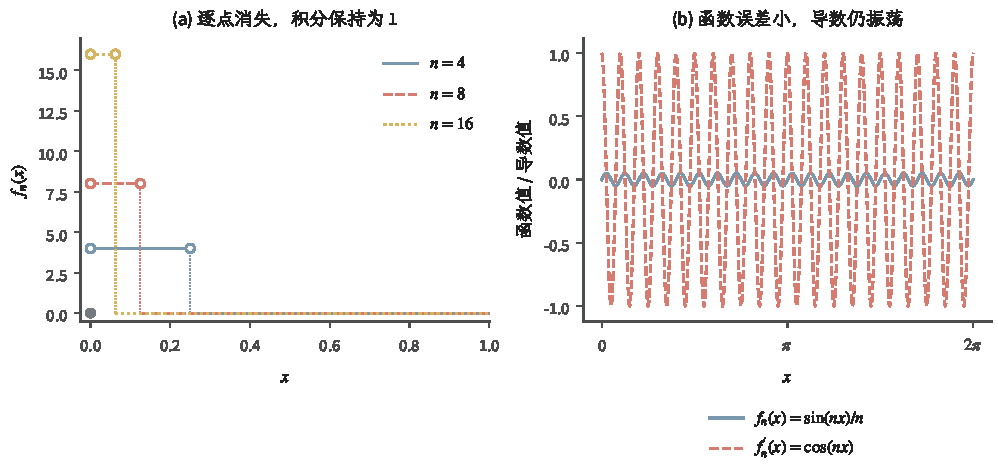
\includegraphics[width=\linewidth]{figures/01-mathematical-preliminaries/01-mathematical-language-combinatorics-analysis-optimization/matplotlib/analysis-geometry/analysis-convergence-obstacles.pdf}
 \caption{两种交换运算的障碍。左图的尖峰支撑不断收缩，但高度同步增长，每条曲线的积分仍为$1$；开圆点标出不取的上端点，竖虚线仅提示跳跃。右图取$n=20$，$\sin(nx)/n$的函数幅度很小，导数$\cos(nx)$仍有单位幅度。两图均为按给定函数公式构造的教学示例。}
 \label{fig:analysis-convergence-obstacles}
\end{figure*}
\FloatBarrier


定理~\ref{thm:analysis-monotone-convergence}已在非负积分构造中证明：非负贡献若逐步
增加，积分便保留其极限。它不要求可积统一上界，也允许无穷总量；现在放宽单调性，
再判断还能得到什么保证。

若只保留非负性，不要求逐步增加，还能得到什么？收缩峰已经说明等式可能失败，
但可以留下一个单向不等式。对不收敛的函数列，回用定义~\ref{def:analysis-liminf-limsup}，在每个$x$处用下极限记录尾部信息。
\begin{lemma}[Fatou引理]
\label{lem:analysis-fatou}
若$f_n:X\to[0,\infty]$可测，则
\begin{equation}
  \int_X\liminf_{n\to\infty}f_n\,\mathrm{d}\mu
  \leq
  \liminf_{n\to\infty}\int_Xf_n\,\mathrm{d}\mu.
\label{eq:analysis-fatou}
\end{equation}
\end{lemma}
\begin{proof}
令$g_n=\inf_{k\geq n}f_k$。则$g_n$可测， $0\leq g_n\uparrow\liminf_k f_k$。由单调收敛定理，
\[   \int\liminf_k f_k\,\mathrm{d}\mu   =   \lim_{n\to\infty}\int g_n\,\mathrm{d}\mu. \]
对每个$k\geq n$都有$g_n\leq f_k$，故
\[   \int g_n\,\mathrm{d}\mu   \leq   \inf_{k\geq n}\int f_k\,\mathrm{d}\mu. \]
令$n\to\infty$便得到式~\eqref{eq:analysis-fatou}。
\end{proof}

Fatou引理通常只给一个方向，因为积分可能在极限中损失质量。对上述收缩峰$f_n$， 左边为$0$，右边为$1$，不等式严格成立。
非负条件也不能直接删除。若改取$u_n=-n\mathbb I_{(0,1/n)}$，则
$\liminf_n u_n=0$处处成立，而$\int u_n=-1$；原不等式会变成错误的$0\leq-1$。
若另有共同的可积下界$h$使$u_n\geq h$，则可以对$u_n-h\geq0$应用Fatou，
再移去有限的$\int h$。可积下界是可用的推广条件，不是无条件允许负值。

\subsubsection{可积支配与积分交换}

若函数会振荡或取负值，单调收敛不适用，Fatou的单向不等式又不足以交换极限。
另一种控制方法是用\emph{同一个可积函数}限制所有逼近的绝对值；它不要求变化单调，
而是阻止越来越高的峰在越来越窄的区域里藏住质量。
\begin{theorem}[支配收敛定理]
\label{thm:analysis-dominated-convergence}
设$f_n,f:X\to\mathbb{R}$可测，$f_n\to f$几乎处处，并且存在非负可积函数$g$使
$|f_n|\leq g$几乎处处对所有$n$成立，则$f$可积，而且
\[   \lim_{n\to\infty}\int_Xf_n\,\mathrm{d}\mu   =   \int_Xf\,\mathrm{d}\mu. \]
此外，$\int|f_n-f|\,\mathrm{d}\mu\to0$。
\end{theorem}
\begin{proof}
把收敛或控制条件失效的可测零测集的可数并记为$N$，并将$f_n,f,g$在$N$上都改为
$0$。这些函数仍可测且积分不变，因而下述关系可以按逐点意义使用。
由$|f_n|\leq g$并取逐点极限可得$|f|\leq g$几乎处处，所以$f$可积。函数$g+f_n$与$g-f_n$均非负。对它们分别使用Fatou引理，
\begin{align*}
  \int g+\int f
  &\leq
  \int g+\liminf_{n\to\infty}\int f_n,\\
  \int g-\int f
  &\leq
  \int g-\limsup_{n\to\infty}\int f_n.
\end{align*}
由于$\int g<\infty$，可以从两边减去它，得到
\[   \int f   \leq\liminf_n\int f_n   \leq\limsup_n\int f_n   \leq\int f. \]
故积分收敛到$\int f$。

最后，$|f_n-f|\to0$几乎处处，且 $|f_n-f|\leq2g$。再对非负函数$|f_n-f|$应用刚证明的积分交换结论，得到 $\int|f_n-f|\,\mathrm{d}\mu\to0$。
\end{proof}

收缩峰$f_n=n\mathbb{I}_{(0,1/n)}$不存在满足条件的可积控制函数。
若$g\geq f_n$几乎处处对每个$n$成立，先把可数个例外集并为$N$。
对$x\in(0,1/4)\setminus N$取$n=\lfloor1/(2x)\rfloor$，
则$n<1/x$且$n\geq1/(4x)$，从而$g(x)\geq f_n(x)=n\geq1/(4x)$。
这个下界在$0$附近不可积，说明失效的是统一可积控制，而不是逐点极限。

贡献还可能逃向无穷远。在$\mathbb R$上取$f_n=\mathbb I_{[n,n+1)}$，
则$f_n\to0$处处成立，积分却恒为$1$。若有共同支配$g$，它须在
$[1,\infty)$上几乎处处至少为$1$，不可能可积。
可积支配同时排除这种向远处移动和前面的局部集中；单纯给出统一常数上界，
在无限测度空间上还不够。

反过来，在$(0,1)$上取$f_n(x)=x^n/\sqrt x$，则逐点趋于零，
且$|f_n|\leq x^{-1/2}$，右侧已知可积。DCT给出$\int f_n\to0$；
直接积分得到$1/(n+1/2)$，核对了结论。支配函数可以无界，
需要有限的是它的积分，而不是普通上确界。

交换符号之前可以按表~\ref{tab:analysis-interchange-conditions}核对实际使用的定理。
“有极限”只提供一个候选函数，附加条件才保证整体量在取极限时被保留下来。

\begin{table*}[htbp]
 \centering\small
 \begin{tabularx}{\linewidth}{@{}lXX@{}}
 \toprule
 结果 & 核对的条件 & 可得到的结论\\
 \midrule
 单调收敛 & 非负可测函数逐点或几乎处处递增 & 极限与积分相等，允许无穷值\\
 Fatou引理 & 非负可测函数列 & 先取下极限再积分，不超过先积分再取下极限的结果\\
 支配收敛 & 几乎处处收敛，且共用一个可积绝对上界 & 积分可交换极限，并有$\int|f_n-f|\,\mathrm d\mu\to0$\\
 Tonelli定理 & $\sigma$有限乘积测度上的非负可测函数 & 交换积分次序，允许无穷值\\
 Fubini定理 & $\sigma$有限乘积测度上的绝对可积函数 & 交换积分次序，并得到有限积分\\
 \bottomrule
 \end{tabularx}
 \caption{极限与积分、积分与积分之间的交换条件。表中的测度、可测性和统一控制属于结论的假设。}
 \label{tab:analysis-interchange-conditions}
\end{table*}

\subsubsection{参数求导与积分交换}

给定参数以后，$g(\cdot,\theta)$是一个函数；让参数接近$\theta_0$时，差商形成一族
逼近函数。因此积分号下求导同时使用第~\ref{sec:analysis-local-models}节的微分、
第~\ref{sec:analysis-integration-average}节的积分，以及刚证明的支配收敛，不能只由
各点偏导数存在就交换运算。


设
\[   G(\theta)=\int_X g(x,\theta)\,\mathrm{d}\mu(x). \]
形式上希望把导数移入积分号：
\[   G'(\theta)   \stackrel{?}{=}   \int_X\frac{\partial g}{\partial\theta}(x,\theta)\,\mathrm{d}\mu(x). \]
真正需要交换的是差商的极限与积分。固定$\theta_0$，设对每个$\theta\in I$，
$x\mapsto g(x,\theta)$可测，其中$I$是包含$\theta_0$的开区间，并且
$g(\cdot,\theta_0)$可积。假设存在一个可测零测集$N$，使每个$x\notin N$处的
$\theta\mapsto g(x,\theta)$在整个$I$内可微；对每个$\theta$，
偏导数作为$x$的函数可测，并且存在非负可积函数$h$使
\begin{equation}
  \left|
    \frac{\partial g}{\partial\theta}(x,\theta)
  \right|
  \leq h(x)
  \quad
  \text{对所有$x\notin N$及所有$\theta\in I$成立},
\label{eq:analysis-parameter-derivative-domination}
\end{equation}
这里$N$和$h$都不能随参数$\theta$改变；参数不可数，不能靠取所有参数例外集的并
自动获得一个零测集。中值定理先给出
$|g(x,\theta)-g(x,\theta_0)|\leq|\theta-\theta_0|h(x)$，
所以$I$中每个$g(\cdot,\theta)$都可积，$G$在邻域内有有限值。
对非零$t$且$\theta_0+t\in I$，令
\[
 q_t(x)=\frac{g(x,\theta_0+t)-g(x,\theta_0)}{t}.
\]
中值定理又给出$|q_t(x)|\leq h(x)$于$X\setminus N$。
差商在那里趋于$\partial g/\partial\theta(x,\theta_0)$。
对任意非零序列$t_n\to0$应用支配收敛，得到同一个积分极限；
由实数极限的序列判据，这就是$t\to0$的双侧极限。因此
\begin{equation}
  G'(\theta_0)
  =
  \int_X
  \frac{\partial g}{\partial\theta}(x,\theta_0)
  \,\mathrm{d}\mu(x).
\label{eq:analysis-differentiate-under-integral}
\end{equation}
条件~\eqref{eq:analysis-parameter-derivative-domination}是一个便于核对的充分条件； 更一般的版本可以直接控制差商，或使用其他一致可积条件。

例如令$g(x,\theta)=e^{-\theta x}$，$x\in[0,\infty)$、$\theta>0$，
并用Lebesgue测度积分。固定$\theta_0>0$后取
$I=(\theta_0/2,3\theta_0/2)$，则
$|\partial_\theta g|=xe^{-\theta x}\leq xe^{-\theta_0x/2}=:h(x)$。
分部积分给出$\int_0^\infty h(x)\,\mathrm dx=4/\theta_0^2<\infty$，
没有需要删除的例外点，故
$G'(\theta_0)=-\int_0^\infty xe^{-\theta_0x}\,\mathrm dx=-1/\theta_0^2$，
与$G(\theta)=1/\theta$的直接求导一致。
若把参数范围放大到任意接近零的正数，便不能沿用这个固定的控制函数；
交换结论所需的是所考察参数点附近的统一控制。

\begin{example}[参数积分中的控制函数失效]
\label{ex:analysis-parameter-integral-failure}
下面考察参数域边界处对应的右求导问题。对$\theta\geq0$与$x\in(0,1)$，定义
\[   g(x,\theta)   =
\begin{cases}     \dfrac{\theta x}{x^2+\theta^2}, & \theta>0,\\[5pt]     0, & \theta=0.
\end{cases} \]
每个固定$x>0$处关于$\theta$的右偏导数都等于$1/x$，但$1/x$在$(0,1)$上不可积。
直接积分得到
\[   G(\theta)   =   \frac{\theta}{2}   \log\left(\frac{1+\theta^2}{\theta^2}\right)   \quad(\theta>0),   \qquad G(0)=0. \]
于是$G(\theta)/\theta$在$\theta\downarrow0$时发散，$G$在$0$处没有有限右导数。积分内的
逐点右导数虽然存在，却缺少统一可积控制；因此这里不能交换右求导与积分。
\end{example}

\section{本章小结}
\label{sec:analysis-summary}

无限过程需要同时说明对象、结构与控制条件。距离比较点与点，测度为集合赋权，
二者分别决定收敛与累计的含义。测度完备化处理零测集的子集，度量完备性保证柯西
点列的极限留在空间内；它们承担不同职责。部分和和更新迭代都产生序列，单步误差
趋零不能替代尾和控制，而统一压缩把几何尾和落实为解的存在、唯一和停止误差。

固定一个函数以后，连续性控制输入扰动，微分提供局部线性模型，二阶信息与Taylor
余项说明曲率及近似损失。隐函数定理把方程的局部解建立为可微函数，使解导数与
最优值的包络导数能够区分。尖点、跳跃和替代更新信号又说明，真实导数、广义梯度
与人为指定的反向信号必须分别判断。

整体累计依赖可测范围和权重。简单函数把积分还原为有限贡献，单调逼近进入一般
非负函数，绝对可积性排除正负无穷相消；积分只有在总权重为$1$或完成归一化后才是
平均。乘积测度、换元与边界公式各自改变累计的对象或表示，积分次序、体积修正与
边界项都有明确条件，不能由有限和的操作习惯直接代替。

函数列仍是序列，但逐点、一致与积分误差控制不同内容。统一逼近能够保留连续性，
却不自动保留导数；非负单调性或共同可积支配则控制极限与积分的关系。积分号下求导
把这两条线结合起来：差商必须既趋向导数，又有足够的积分控制。后续使用这些工具时，
应先辨认当前对象及所需保证，再核对定义域、光滑性、可积性与统一条件。
第~\ref{chap:optimization}章据此研究最优性与求解，第~\ref{chap:functional-analysis-and-approximation}章
进一步研究函数空间中的表示、逼近和稳定性。

\chapter{最优化}
\label{chap:optimization}

第~\ref{chap:mathematical-analysis}章说明了函数在一点附近怎样变化。本章要把这些局部信息
用于一个整体问题：在所有允许的参数中，怎样判断某个参数已经足够好，又怎样逐步找到它？
贯穿全章的对象是带正则项的最小二乘
\begin{equation}
  F(\bm{w})
  =
  \frac{1}{2n}\lVert \bm{X}\bm{w}-\bm{y}\rVert_2^2
  +\frac{\lambda}{2}\lVert\bm{w}\rVert_2^2,
  \qquad
  \bm{X}\in\mathbb{R}^{n\times d},\quad \lambda\geq 0,
  \label{eq:opt-regularized-least-squares}
\end{equation}
以及线性资源约束
\begin{equation}
  \bm{A}\bm{w}=\bm{b},\qquad
  \bm{G}\bm{w}\leq\bm{h}.
  \label{eq:opt-linear-resource-constraints}
\end{equation}
式~\eqref{eq:opt-regularized-least-squares}与第~\ref{chap:sets-functions-and-proofs}章的
式~\eqref{eq:prelim-regularized-least-squares}是同一个目标的矩阵写法。正则项限制参数
规模，约束则直接排除超出预算的候选；两者看似都在“限制模型”，却改变了不同的数学对象。

本章先说明解的存在与曲率如何决定局部信息的效力，再用约束、乘子、对偶和松弛建立
可核验的最优性证书；在认清目标与保证后，讨论光滑迭代、代理上界，以及非光滑项和不完整
梯度需要的更新方式。分块、多目标和双层问题不是
一条由旧到新的算法路线，而是三种不同的问题组织方式。读完本章，读者应能判断一个优化结论
依赖哪些条件，并能指出条件失效时究竟失去了存在性、全局性、唯一性还是收敛速度。

\section{目标、解与曲率}
\label{sec:opt-objectives-solutions-curvature}

求解算法之前，需要分清三件事：问题是否有解、怎样认出最优点，以及局部信息能否保证全局最优。
存在性主要依赖目标与可行域的闭合性质；凸性和其他曲率条件则决定驻点、解的唯一性与误差界。
这些是后面各种算法共用的前提，不是三种求解方法。

\subsection{问题设定与解的性质}
\label{sec:opt-problem-and-solutions}

\subsubsection{可行性、最优性与近似标准}

一个优化问题必须同时给出目标函数、变量和可行域。记
\[
  \min_{\bm{w}\in C}F(\bm{w}),\qquad
  C=\{\bm{w}\in\mathbb{R}^d:
  \bm{A}\bm{w}=\bm{b},\ \bm{G}\bm{w}\leq\bm{h}\}.
\]
若$C=\varnothing$，问题\term{不可行}（infeasible）；若$C\neq\varnothing$但
$\inf_{\bm{w}\in C}F(\bm{w})=-\infty$，问题\term{无下界}（unbounded below）。
只有可行且有有限下界，才值得继续问下确界是否由某个点达到。

\begin{definition}[全局解、局部解与无约束驻点]
\label{def:opt-solutions-stationarity}
设$C\subseteq\mathbb R^d$非空，$F:C\to\mathbb R$。\term{全局最优解}（global minimizer）$\bm{w}^{\star}\in C$满足
$F(\bm{w}^{\star})\leq F(\bm{w})$对所有$\bm{w}\in C$成立。\term{局部最优解}
（local minimizer）要求存在$r>0$，使该不等式对所有
$\bm w\in C\cap B(\bm w^\star,r)$成立。
无约束可微问题的\term{驻点}（stationary point）满足
$\nabla F(\bm{w})=\bm{0}$。驻点只是局部一阶变化消失，可能是极小点、极大点或
第~\ref{sec:analysis-second-order-curvature}节所说的微分鞍点。
\end{definition}
给定$\varepsilon>0$和可行候选$\widehat{\bm w}\in C$，若
\[
  F(\widehat{\bm{w}})-\inf_{\bm{w}\in C}F(\bm{w})\leq\varepsilon,
\]
就称$\widehat{\bm{w}}$为目标值意义下的$\varepsilon$近似解。对无约束可微问题，
另一种常见标准是
$\lVert\nabla F(\widehat{\bm{w}})\rVert_2\leq\varepsilon$；在没有额外曲率条件时，
这两种近似不能互换。一般约束问题的精确最优点也可能有非零梯度，此时应改用投影梯度、
可行方向导数或KKT残差等同时反映可行性与驻点性的标准。

\subsubsection{目标值、参数与预测误差}
\label{sec:opt-error-objects}

前面的目标值近似标准只比较目标与最优值之间的差距。评价同一个近似参数时，还可以关心它离某个参照参数多远，
或者它的预测发生了多大变化。这三个问题要分别选择误差对象。
下面暂取$C=\mathbb{R}^d$，不加资源约束，以式~\eqref{eq:opt-regularized-least-squares}为目标。
令$F^\star=\inf_{\bm{w}\in\mathbb{R}^d}F(\bm{w})$；若选定一个最小点
$\bm{w}^\star$，则
\[
  F(\widehat{\bm{w}})-F^\star,\qquad
  \lVert\widehat{\bm{w}}-\bm{w}^\star\rVert_2,\qquad
  \left(
    \frac{1}{n}\sum_{i=1}^{n}
    \bigl(
      \widehat{\bm{w}}^{\top}\bm{x}_i
      -(\bm{w}^\star)^{\top}\bm{x}_i
    \bigr)^2
  \right)^{1/2}
\]
分别是目标值误差、参数误差和在给定样本输入上的预测误差。最小点不唯一时，参数误差还
需要指定参照解，或改成到最小点集合的距离。三种误差衡量不同对象，彼此能否控制取决于
目标曲率、数据矩阵和参数化；一个误差较小不能无条件推出另两个也较小。

例如，在$n=1$、$\bm{x}_1=(1,0)^\top$、$y_1=0$、$\lambda=0$时，
目标函数为$F(w_1,w_2)=w_1^2/2$。参照解$(0,0)$与参数$(0,100)$的目标值都为$0$，
在这个样本输入上的预测也相同，参数距离却是$100$。差别来自目标和当前观测都没有约束
第二个坐标；并不是把目标误差算得更精确就能补回这项信息。

\subsubsection{解的存在、唯一与稳定性}

若$C\subseteq\mathbb{R}^d$非空且紧，$F:C\to\mathbb{R}$连续，则
定理~\ref{thm:analysis-extreme-value}保证$F$在$C$上达到全局最小值。这里直接复用
第~\ref{chap:mathematical-analysis}章的极值存在结论。

可行域不紧时，目标本身也可能阻止最小化序列逃向无穷远。
\begin{definition}[强制性与下半连续性]
\label{def:opt-coercive-lower-semicontinuous}
设$C\subseteq\mathbb R^d$，$F:C\to(-\infty,+\infty]$。若沿$C$中的任意序列，
$\lVert\bm{w}\rVert_2\to\infty$时$F(\bm{w})\to\infty$，称$F$是
\term{强制的}（coercive）。$F$在$C$上\term{下半连续}
（lower semicontinuous）要求对每个收敛序列
$\bm{w}^{(k)}\to\bm{w}$都有
\[
  F(\bm{w})\leq\liminf_{k\to\infty}F(\bm{w}^{(k)}).
\]
其中序列与极限点均属于$C$。
\end{definition}
连续性并不是存在性证明所需的最弱条件。下半连续性允许函数值在极限点向下跳，
却不允许极限点的函数值突然高于邻近值。等价地，每个
下水平集$\{\bm{w}\in C:F(\bm{w})\leq a\}$在$C$的相对拓扑中都是闭集。

设$C$非空且闭，$F:C\to(-\infty,+\infty]$下半连续、强制，并且不恒为
$+\infty$且从不取$-\infty$。取$\bar{\bm{w}}\in C$使
$F(\bar{\bm{w}})<+\infty$，再把最小化序列限制到下水平集
\[
  K=\{\bm{w}\in C:F(\bm{w})\leq F(\bar{\bm{w}})\}.
\]
若$\inf_C F=F(\bar{\bm{w}})$，则$\bar{\bm{w}}$已经是最小点；否则
$\inf_C F<F(\bar{\bm{w}})$，任一最小化序列从某项起都落入$K$，可以只保留这段尾序列。
强制性使$K$有界，下半连续性与$C$的闭性使$K$闭，故$K$在有限维空间中紧。该尾序列
有子列收敛到$\bm{w}^{\star}\in K$，而下半连续性给出
$F(\bm{w}^{\star})\leq\liminf_kF(\bm{w}^{(k)})=\inf_C F$。因此下确界达到。
这个证明也指出各条件的职责：强制性阻止序列逃向无穷远，闭性保留可行极限，下半连续性
把目标值比较传到极限点。
当$\lambda>0$时，式~\eqref{eq:opt-regularized-least-squares}满足
$F(\bm{w})\geq\lambda\lVert\bm{w}\rVert_2^2/2$，所以即使可行域无界也不会沿参数
无穷大的方向降低目标。

存在不等于唯一。若$\lambda=0$且$\bm{X}$有非零零空间向量$\bm{v}$，那么
$F(\bm{w}+t\bm{v})=F(\bm{w})$，最小点可能形成一条直线。即使唯一，数值问题也可能
非常敏感。例如令$0<\epsilon\ll1$并考虑
\[
  f_b(w_1,w_2)=\frac12(\epsilon w_1^2+w_2^2)-bw_1.
\]
它对每个$b$都有唯一最小点$(b/\epsilon,0)$，但$b$改变$\Delta b$会使第一坐标改变
$\Delta b/\epsilon$。更一般的二次目标具有如下曲率矩阵：
\[
  \bm{H}=\frac{1}{n}\bm{X}^{\top}\bm{X}+\lambda\bm{I}
\]
当$\bm{H}\succ\bm{0}$时，若线性项受到加性扰动$\delta\bm{g}$，相应解变化满足
\[
  \lVert\delta\bm{w}\rVert_2
  \leq
  \frac{1}{\lambda_{\min}(\bm{H})}
  \lVert\delta\bm{g}\rVert_2.
\]
因此$1/\lambda_{\min}(\bm{H})$控制固定尺度加性扰动的绝对放大；经过目标和变量尺度
归一化后，条件数
$\kappa(\bm{H})=\lambda_{\max}(\bm{H})/\lambda_{\min}(\bm{H})$
才刻画相对病态程度。例如$\bm{H}=\epsilon\bm{I}$的条件数为$1$，但绝对扰动仍会被
放大$1/\epsilon$倍。唯一性回答“解有几个”，敏感性还取决于所采用的扰动尺度，
不能只由唯一性或条件数笼统判断。

\subsection{凸集与凸函数}
\label{sec:opt-convexity}

\subsubsection{线段、曲率与全局下界}

约束只告诉我们哪些点允许使用；还要问两个可行点之间能否连续移动而始终可行。
\begin{definition}[凸集与凸函数]
\label{def:opt-convex-set-function}
集合$C\subseteq\mathbb R^d$为\term{凸集}（convex set），是指对任意
$\bm{u},\bm{v}\in C$和$\theta\in[0,1]$，
$\theta\bm{u}+(1-\theta)\bm{v}\in C$。线性等式、线性不等式和范数球的解集都是凸集，
它们的交集仍为凸集，所以式~\eqref{eq:opt-linear-resource-constraints}定义凸可行域。

定义在凸集$C$上的函数$f:C\to\mathbb R$若对任意$\bm u,\bm v\in C$和$\theta\in[0,1]$满足
\begin{equation}
  f(\theta\bm{u}+(1-\theta)\bm{v})
  \leq
  \theta f(\bm{u})+(1-\theta)f(\bm{v}),
  \label{eq:opt-convex-function}
\end{equation}
就称为\term{凸函数}（convex function）。若$-f$凸，则称$f$凹。
\end{definition}
凸函数的函数图像位于任意弦段下方，因此局部低点
不会被更远处的谷底击败\scite{math-boyd2004convex}

\begin{theorem}[凸函数的一阶与二阶判据]
\label{thm:opt-convexity-criteria}
设$C$为开凸集。可微函数$f:C\to\mathbb{R}$凸，当且仅当对任意
$\bm{u},\bm{v}\in C$，
\begin{equation}
  f(\bm{v})\geq f(\bm{u})
  +\langle\nabla f(\bm{u}),\bm{v}-\bm{u}\rangle.
  \label{eq:opt-first-order-convexity}
\end{equation}
若$f$二阶可微，则这又等价于
$\nabla^2f(\bm{w})\succeq\bm{0}$对所有$\bm{w}\in C$成立。
\end{theorem}

\begin{proof}
若$f$凸，令$\phi(t)=f(\bm{u}+t(\bm{v}-\bm{u}))$。由凸性，
$[\phi(t)-\phi(0)]/t\leq\phi(1)-\phi(0)$。令$t\downarrow0$便得
式~\eqref{eq:opt-first-order-convexity}。反过来，令
$\bm{z}=\theta\bm{u}+(1-\theta)\bm{v}$，分别把一阶不等式用于
$(\bm{z},\bm{u})$和$(\bm{z},\bm{v})$，乘以$\theta$与$1-\theta$后相加，
线性项抵消，得到式~\eqref{eq:opt-convex-function}。

若$f$凸，把一阶判据用于$\bm{w}$与$\bm{w}+t\bm{v}$，再对$t$求二阶局部极限，
得到$\bm{v}^{\top}\nabla^2f(\bm{w})\bm{v}\geq0$。反之，沿任意线段定义
$\phi(t)$，则
$\phi''(t)=(\bm{v}-\bm{u})^{\top}\nabla^2f(\bm{u}+t(\bm{v}-\bm{u}))
(\bm{v}-\bm{u})\geq0$，一元函数$\phi$凸，故$f$凸。
\end{proof}

反复应用二点凸性可得\term{Jensen不等式}（Jensen's inequality）。若
$\alpha_i\geq0$且$\sum_i\alpha_i=1$，则
\begin{equation}
  f\left(\sum_{i=1}^m\alpha_i\bm{w}_i\right)
  \leq\sum_{i=1}^m\alpha_i f(\bm{w}_i).
  \label{eq:opt-jensen}
\end{equation}
归纳步骤把前$m-1$个点先归一化为一个加权平均，再与第$m$个点应用二点凸性。
这个证明也说明非负和归一化不是装饰条件；允许负权重后，组合点可能落到凸包之外，
因而不能再由凸性保证Jensen不等式。

凸性还把最优性变成可核验的一阶条件。若$f$可微且凸，则
$\nabla f(\bm{w}^{\star})=\bm{0}$代入式~\eqref{eq:opt-first-order-convexity}
便得$f(\bm{v})\geq f(\bm{w}^{\star})$。因此凸问题的驻点是全局最小点。
图~\ref{fig:opt-convex-chord-tangent}同时画出这两侧的界。弦在图像上方，源于二点凸组合；
切线在图像下方，源于可微凸函数的一阶判据。二者夹住函数，却来自不同的比较对象，
不能把某点处的切线误当作连接两个函数值的弦。
\begin{figure}[htbp]
 \centering
 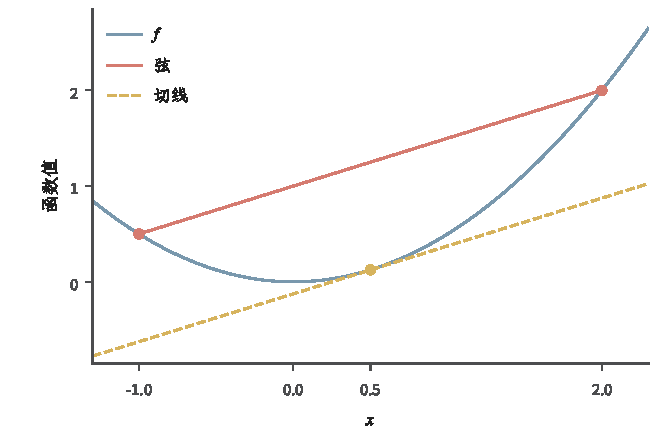
\includegraphics[width=\linewidth]{figures/math-preparation/reader-revision-analysis/optimization-convex-chord-tangent.pdf}
 \caption{$f(x)=x^2/2$的弦与切线。蓝线为函数，红线连接$u=-1$与$v=2$的函数值，
 在这两个输入之间给出弦上界；黄虚线是在$x_0=1/2$处的一阶仿射下界，适用于整个实线。
 红线的上界只在其端点之间使用，切线下界来自凸性。图为解析教学示例。}
 \label{fig:opt-convex-chord-tangent}
\end{figure}


\begin{definition}[严格凸函数]
\label{def:opt-strict-convexity}
设$C$凸，$f:C\to\mathbb R$。若式~\eqref{eq:opt-convex-function}对所有
$\bm u\neq\bm v$及$0<\theta<1$严格成立，则称$f$严格凸。
\end{definition}
严格凸保证最小点至多一个，却不给统一曲率下界。强凸性则要求弦段与函数之间至少留出一个与距离平方成比例的间隔。
这个定义可以用于非光滑正则项，也可以使用欧氏范数以外的范数。

\begin{definition}[相对于范数的强凸性]
\label{def:opt-strong-convexity}
设$C$是实赋范空间中的凸集，$f:C\to\mathbb{R}$，$\mu>0$。若对任意
$\bm{u},\bm{v}\in C$和$\theta\in[0,1]$都有
\begin{equation}
 f(\theta\bm{u}+(1-\theta)\bm{v})
 \leq\theta f(\bm{u})+(1-\theta)f(\bm{v})
 -\frac{\mu}{2}\theta(1-\theta)\lVert\bm{u}-\bm{v}\rVert^2,
 \label{eq:opt-norm-strong-convexity}
\end{equation}
则称$f$相对于$\lVert\cdot\rVert$是\term{$\mu$强凸}（$\mu$-strongly convex）的。
\end{definition}

在欧氏空间的开凸集上，若$f$可微，强凸性等价于一阶下界
\begin{equation}
  f(\bm{v})\geq f(\bm{u})+
  \langle\nabla f(\bm{u}),\bm{v}-\bm{u}\rangle
  +\frac{\mu}{2}\lVert\bm{v}-\bm{u}\rVert_2^2.
  \label{eq:opt-first-order-strong-convexity}
\end{equation}
可用定理~\ref{thm:opt-convexity-criteria}对
$f(\bm{w})-\mu\lVert\bm{w}\rVert_2^2/2$应用凸性判据得到这一等价关系；若$f$二阶可微，
它又等价于$\nabla^2f(\bm{w})\succeq\mu\bm{I}$。一般范数的平方未必是欧氏二次型，
因此不能把这一Hessian写法直接当作所有范数下的定义。
例如$|x|+\mu x^2/2$虽在$0$处不可微，仍相对于绝对值范数$\mu$强凸：绝对值部分满足
凸性，二次部分恰好提供式~\eqref{eq:opt-norm-strong-convexity}中的距离平方间隔。

一阶算法还需要防止梯度随位移过快改变。
\begin{definition}[欧氏梯度光滑性]
\label{def:opt-smoothness}
设$C\subseteq\mathbb R^d$开且凸，$f:C\to\mathbb R$可微，$L\geq0$有限。
$f$为\term{$L$光滑}（$L$-smooth），是指对任意$\bm u,\bm v\in C$，梯度满足
$\lVert\nabla f(\bm{u})-\nabla f(\bm{v})\rVert_2
\leq L\lVert\bm{u}-\bm{v}\rVert_2$。
\end{definition}
这里对梯度使用同一Lipschitz常数。强凸给下曲率，光滑给上曲率；$x^4$严格凸但
不在全实线上强凸，也不在全实线上具有有限的光滑常数。

\subsection{较弱曲率与非凸结构}
\label{sec:opt-weaker-curvature}

凸性同时约束所有线段上的函数值，有时比具体求解所需的条件更强。
下面分开讨论两种放宽：弱凸允许负曲率但限制其大小，PL条件直接把梯度大小与目标差联系起来。
它们服务于不同推导，不应把名称看成从凸到非凸的单一强弱序列。

\subsubsection{弱凸与补足曲率}

强凸同时控制函数形状和误差。实际目标可能不凸，却仍有足够结构支持算法分析。
\begin{definition}[欧氏空间中的弱凸性]
\label{def:opt-weak-convexity}
设$f:\mathbb{R}^d\to\mathbb{R}\cup\{+\infty\}$是适当函数，即不恒为$+\infty$，
且$\rho\geq0$。若
$\bm{w}\mapsto f(\bm{w})+\rho\lVert\bm{w}\rVert_2^2/2$是凸函数，
则称$f$是\term{$\rho$弱凸}（$\rho$-weakly convex）的。取值$+\infty$可以用来表示不可行点。
\end{definition}
若$f$在开凸定义域上二阶可微，这等价于
$\nabla^2f(\bm{w})\succeq-\rho\bm{I}$：负曲率可以存在，但有统一下界。
当$\rho>0$且$0<\eta<1/\rho$时，对任意中心$\bm{z}$，邻近子问题的目标
\[
  f(\bm{w})+\frac{1}{2\eta}\lVert\bm{w}-\bm{z}\rVert_2^2
\]
是$(1/\eta-\rho)$强凸函数；若$\rho=0$，任意$\eta>0$都具有同样的补足曲率作用。
这正是弱凸性与第~\ref{sec:opt-nonsmooth-proximal}节邻近方法的联系。补入二次曲率
只让这个子问题更易控制，并没有把原函数变成凸函数；弱凸目标仍可有局部极小点和鞍点，
也不保证求得原问题的全局最优解。

例如$f(x)=\cos x$的二阶导数是$-\cos x\geq-1$，所以它是$1$弱凸的，
但仍有无穷多个局部低点。弱凸性限制谷之间最坏的负曲率，并未消除这些谷。
若在当前位置附近加上足够大的二次惩罚，邻近子问题会得到唯一解；改变当前位置后，
所解的却是另一个邻近子问题，不能据此声称原函数只有一个最小点。

\subsubsection{Polyak--Łojasiewicz条件}

\term{Polyak--Łojasiewicz条件}（PL condition）不约束函数图像必须凸，而用梯度大小控制
距离最优值还有多少差距。
\begin{definition}[Polyak--Łojasiewicz条件]
\label{def:opt-pl-condition}
设$f:\mathbb{R}^d\to\mathbb{R}$可微，$f^\star=\inf_{\bm{w}}f(\bm{w})> -\infty$。
若存在$\mu>0$，使任意$\bm{w}$满足
\begin{equation}
  \frac{1}{2}\lVert\nabla f(\bm{w})\rVert_2^2
  \geq \mu\bigl(f(\bm{w})-f^{\star}\bigr),
  \qquad \mu>0.
  \label{eq:opt-pl-condition}
\end{equation}
则称$f$满足常数为$\mu$的PL条件。
\end{definition}
该条件把小梯度与小目标误差联系起来。强凸可推出PL条件：对$\mu$强凸可微函数，把强凸
下界右侧关于$\bm{v}$最小化，得到
\[
  f^\star\geq
  f(\bm{w})-\frac{1}{2\mu}\lVert\nabla f(\bm{w})\rVert_2^2,
\]
移项正是式~\eqref{eq:opt-pl-condition}。这个推导使用全局强凸下界；只有局部Hessian
正定时，不能直接得到全域PL条件。反过来，PL函数可以有多个最小点。

同一个低维族能显示这些性质各自控制什么。令
\[
  f_a(x_1,x_2)=\frac12(x_1+x_2)^2+\frac{a}{2}(x_1-x_2)^2.
\]
当$a>0$时函数强凸；$a=0$时它凸且满足PL条件，但整条直线$x_1+x_2=0$都是最小点；
$a<0$时函数弱凸却无下界。若限制在紧可行域上，$a<0$时仍有最小点，但驻点
$(0,0)$可能是鞍点。这个例子说明弱凸、PL和强凸不是一条简单的强弱链：弱凸限制最坏负
曲率，PL控制梯度与目标误差，强凸还控制参数距离与唯一性。

PL条件也确实可以出现在非凸函数中。考虑
\[
  f(x,y)=x^2+2\sin^2x.
\]
它与$y$无关，因而最小点不唯一。其一阶导数为
$\partial f/\partial x=2(x+\sin 2x)$；当$x>0$时，若$x\leq1$则两项均非负，
若$x>1$则$x+\sin2x\geq x-1>0$，负半轴由奇对称性处理，所以导数只在$x=0$时
为零。比值
\[
  R(x)=\frac{\lVert\nabla f(x,y)\rVert_2^2}{2f(x,y)}
\]
在$x\neq0$时为正，并且$x\to0$时趋于$6$，$|x|\to\infty$时趋于$2$。
把两端之外的剩余区域限制为紧集，连续函数$R$在其中有正下界，故某个$\mu>0$使
式~\eqref{eq:opt-pl-condition}成立。另一方面，
$\partial^2 f/\partial x^2=2+4\cos2x$在某些点为负，所以$f$并不凸；该二阶导数
下界为$-2$、绝对值上界为$6$，又说明它同时是$2$弱凸且$6$光滑。这个例子不能推出
所有弱凸函数都满足PL条件，它只表明非凸性本身不排斥目标值的梯度控制。

式~\eqref{eq:opt-regularized-least-squares}的Hessian矩阵为
$\bm{X}^{\top}\bm{X}/n+\lambda\bm{I}$。当$\lambda>0$时，正则项把所有缺失曲率的
方向至少抬高到$\lambda$，因而目标$\lambda$强凸。若$\lambda=0$且$\bm{X}$不满列秩，
驻点仍是全局最优点，但解不唯一；若目标再加入非凸项，驻点甚至不再保证局部最小。

\begin{table*}[htbp]
 \centering\small
 \begin{tabularx}{\linewidth}{@{}lXX@{}}
 \toprule
 条件 & 直接控制什么 & 单凭该条件不能得到什么\\
 \midrule
 凸性 & 全部线段上的弦上界；局部最小点也是全局最小点 & 最小点存在、唯一或统一收敛速率\\
 严格凸性 & 非平凡线段上的严格不等式；最小点至多一个 & 一致正曲率下界，例如$x^4$在原点曲率为零\\
 强凸性 & 函数值相对切平面的二次增长（可微情形） & 梯度光滑性，例如$|x|+\mu x^2/2$仍有尖点\\
 弱凸性 & 最坏负曲率的统一下界 & 驻点全局最优或最小点唯一\\
 PL条件 & 梯度大小控制目标值差 & 凸性或参数解的唯一性\\
 \bottomrule
 \end{tabularx}
 \caption{曲率条件的职责比较。各行针对不同性质，不能排成一条从“弱”到“强”的完整等级。}
 \label{tab:opt-curvature-conditions}
\end{table*}

\section{约束、对偶与最优性证书}
\label{sec:opt-constraints-duality-certificates}

前节的局部驻点标准允许考察任意方向；有资源约束时，降低目标的方向可能不可行。
乘子把可行方向的限制纳入一阶条件，对偶把这些限制转换为目标的下界，松弛则让难以直接求解的问题也能得到可计算的界。
三者共同回答：一个候选解是否可行，以及还可能改善多少。

\subsection{凸几何与仿射下界}
\label{sec:opt-affine-certificates}
把不可行或次优转为可核验的线性不等式，需要先说明分离与支撑；
再把同样的仿射下界语言用于函数，就能理解共轭与对偶中的界来自哪里。

\subsubsection{最近点与线性分离}

\begin{theorem}[闭凸集外一点的严格分离]
\label{thm:opt-projection-separation}
设$C\subseteq\mathbb{R}^d$非空、闭且凸，$\bm{z}\notin C$。则存在
$\bm{a}\neq\bm{0}$和$c\in\mathbb{R}$，使
\[
  \langle\bm{a},\bm{x}\rangle\leq c
  <\langle\bm{a},\bm{z}\rangle
  \quad\text{对所有 }\bm{x}\in C.
\]
\end{theorem}

\begin{proof}
先证明所需最近点的存在性与唯一性。任取$\bm{x}_0\in C$并令
$R=\lVert\bm{z}-\bm{x}_0\rVert_2$。集合
\[
  C_R=C\cap\{\bm{x}:\lVert\bm{z}-\bm{x}\rVert_2\leq R\}
\]
非空、闭且有界，因而在有限维空间中紧。连续函数
$\lVert\bm{z}-\bm{x}\rVert_2^2$在$C_R$上达到最小值；球外各点到$\bm{z}$的
距离大于$R$，而$\bm{x}_0$的距离等于$R$，所以该最小点也是$C$上的最近点。
若$\bm{p}_1,\bm{p}_2$都是最近点，最近距离为$\delta$，则凸性保证其中点属于$C$，且
\[
  \left\lVert\bm{z}-\frac{\bm{p}_1+\bm{p}_2}{2}\right\rVert_2^2
  =
  \frac12\lVert\bm{z}-\bm{p}_1\rVert_2^2
  +\frac12\lVert\bm{z}-\bm{p}_2\rVert_2^2
  -\frac14\lVert\bm{p}_1-\bm{p}_2\rVert_2^2.
\]
当$\bm{p}_1\neq\bm{p}_2$时，右端严格小于$\delta^2$，与最近距离的定义矛盾，故最近点
唯一，记为$\bm{p}$。

对任意$\bm{x}\in C$，
$\bm{p}+t(\bm{x}-\bm{p})\in C$。函数
$q(t)=\lVert\bm{z}-\bm{p}-t(\bm{x}-\bm{p})\rVert_2^2$在$t=0$
处右导数非负，所以
$\langle\bm{z}-\bm{p},\bm{x}-\bm{p}\rangle\leq0$。取
$\bm{a}=\bm{z}-\bm{p}$和$c=\langle\bm{a},\bm{p}\rangle$，则
$\langle\bm{a},\bm{x}\rangle\leq c$，而
$\langle\bm{a},\bm{z}\rangle=c+\lVert\bm{a}\rVert_2^2>c$。
\end{proof}

\begin{definition}[支撑超平面与凸锥]
\label{def:opt-supporting-hyperplane-cone}
设$C\subseteq\mathbb R^d$非空，$\bm a\neq0$。若$C$全部位于
$\{\bm x:\langle\bm a,\bm x\rangle\leq c\}$，并且至少有一点取等号，
则等号超平面称为$C$的\term{支撑超平面}（supporting hyperplane）。
非空集合$K$若对所有$\bm u,\bm v\in K$、$\alpha,\beta\geq0$都有
$\alpha\bm u+\beta\bm v\in K$，称为凸锥。
\end{definition}
具体地说，若$\bm{p}$位于闭凸集$C$的边界，可取一列集外点
$\bm{z}^{(k)}\to\bm{p}$，对每个点应用严格分离并把法向量归一化。单位球的紧性给出
收敛子列，极限法向量$\bm{a}\neq\bm{0}$满足
$\langle\bm{a},\bm{x}\rangle\leq\langle\bm{a},\bm{p}\rangle$对所有
$\bm{x}\in C$成立。这说明边界处至少有一个支撑方向，但边界有棱角时法向量未必唯一。
分离把“点不属于集合”转化为一个线性不等式证书，但它本身不自动给出一般凸问题的强对偶；
还需要闭性或约束资格条件。

对称矩阵集合中的\term{半正定锥}（positive semidefinite cone）
\[
  \mathbb{S}_+^d=\{\bm{M}=\bm{M}^{\top}:
  \bm{v}^{\top}\bm{M}\bm{v}\geq0,\ \forall\bm{v}\}
\]
是凸锥，因为非负线性组合仍保持二次型非负。它也是闭集：若
$\bm{M}^{(k)}\to\bm{M}$且每个$\bm{M}^{(k)}\succeq\bm{0}$，则对任意固定
$\bm{v}$都有
$\bm{v}^{\top}\bm{M}\bm{v}
=\lim_k\bm{v}^{\top}\bm{M}^{(k)}\bm{v}\geq0$。
线性规划的非负正交锥和半正定规划的矩阵约束直接定义凸可行域；标准凸二次规划中的
半正定曲率矩阵则保证目标凸。三者共享的是凸目标与凸可行域的语言。若要进一步统一成
带线性目标的锥规划，还需引入辅助变量，对二次目标作上图或锥提升。

\subsubsection{凸共轭与双共轭}

分离用仿射函数区分一个点与可行集合。对目标函数，也可以收集所有仿射下界：
固定斜率后找最紧的截距，再比较所有斜率能否重建原函数。凸共轭承担这一步。
\begin{definition}[适当函数、有效定义域与约束指标]
\label{def:opt-proper-domain-indicator}
函数$f:\mathbb R^d\to\mathbb R\cup\{+\infty\}$若不恒为$+\infty$，称为适当函数；
它从不取$-\infty$。其\term{有效定义域}（effective domain）为
$\operatorname{dom}f=\{\bm x:f(\bm x)<+\infty\}$。
集合$C$的扩展实值指标函数为$\iota_C(\bm x)=0$（$\bm x\in C$），在其余点取$+\infty$。
\end{definition}
这个指标不是第~\ref{chap:sets-functions-and-proofs}章取$0/1$的指示函数。
它把不允许的点排除出最小化，而不只是给集合成员作标记。
对扩展实值目标，式~\eqref{eq:opt-convex-function}在有限取值的点上检验，
并要求有效定义域凸；这避免在端点权重为零时操作$0\cdot(+\infty)$。
上图集$\operatorname{epi}f=\{(\bm x,r)\in\mathbb R^{d+1}:r\geq f(\bm x)\}$
记录图像以上的全部点；它凸与$f$凸等价，闭与$f$下半连续等价。
\begin{definition}[凸共轭与双共轭]
\label{def:opt-conjugate}
给定适当函数$f:\mathbb R^d\to\mathbb R\cup\{+\infty\}$，其\term{凸共轭}
（convex conjugate）定义为
\begin{equation}
 f^*(\bm y)=\sup_{\bm x\in\mathbb R^d}
            \{\langle\bm y,\bm x\rangle-f(\bm x)\},
 \qquad
 f^{**}(\bm x)=\sup_{\bm y\in\mathbb R^d}
            \{\langle\bm y,\bm x\rangle-f^*(\bm y)\}.
 \label{eq:opt-conjugate-biconjugate}
\end{equation}
两个上确界都在整个$\mathbb R^d$上取。$f^*$允许取$+\infty$；若$f^*\equiv+\infty$，
则$f^{**}\equiv-\infty$，否则$f^{**}$不取$-\infty$，但仍可能取$+\infty$。
\end{definition}
这里$f(\bm x)=+\infty$的点不贡献有限共轭候选。固定斜率$\bm y$时，$f^*(\bm y)$是
让$\langle\bm y,\bm x\rangle-f^*(\bm y)$在全域不超过$f$所需的最小截距修正。
没有任何仿射下界时，这个修正对每个斜率都为无穷。例如$f(x)=-x^2$满足
$f^*(y)=\sup_x\{yx+x^2\}=+\infty$，双共轭因而恒为$-\infty$；适当性本身不能排除这一情形。
由定义立即有\term{Fenchel--Young不等式}
\[
 f(\bm x)+f^*(\bm y)\geq\langle\bm y,\bm x\rangle,
\]
以及$f^{**}\leq f$。共轭是仿射函数族的上确界，因而凸且下半连续；它并非简单把
函数图像交换横纵坐标，也不要求每个上确界都由有限斜率达到。

\begin{theorem}[有限维Fenchel--Moreau定理]
\label{thm:opt-fenchel-moreau}
设$f:\mathbb R^d\to\mathbb R\cup\{+\infty\}$适当、下半连续且凸。
则$f^{**}=f$在全部$\mathbb R^d$上成立，包括$f(\bm x)=+\infty$的点。
因此$f$恰好是全部连续仿射下界的逐点上确界。
\end{theorem}

\begin{proof}
上图集$\operatorname{epi}f=\{(\bm x,r):r\geq f(\bm x)\}$非空、闭且凸。
任取$\bm x_0\in\operatorname{dom}f$及$t_0<f(\bm x_0)$，对上图与其外一点
$(\bm x_0,t_0)$使用定理~\ref{thm:opt-projection-separation}，得到
\[
 \langle\bm a,\bm x_0\rangle+b t_0<c
 \leq\langle\bm a,\bm z\rangle+b r
 \quad\text{对所有 }(\bm z,r)\in\operatorname{epi}f.
\]
上图沿$r$向上无界，故$b\geq0$；若$b=0$，取
$(\bm z,r)=(\bm x_0,f(\bm x_0))$便矛盾，所以$b>0$。
重排得到一个全域仿射下界$\ell_0(\bm z)=\langle\bm p_0,\bm z\rangle-\beta_0\leq f(\bm z)$。
这也保证$f^*(\bm p_0)$有限。

现任取$\bm x$和实数$t<f(\bm x)$，再次严格分离$(\bm x,t)$与上图。
若所得竖直系数$b>0$，立即得到一个仿射下界$\ell$，满足$\ell(\bm x)>t$。
若$b=0$，分离不等式为$\langle\bm a,\bm x\rangle<c\leq\langle\bm a,\bm z\rangle$。
将它与$\varepsilon(r-\ell_0(\bm z))\geq0$相加，得到
\[
 \langle\bm a-\varepsilon\bm p_0,\bm z\rangle+\varepsilon r
 \geq c-\varepsilon\beta_0.
\]
取足够小的$\varepsilon>0$，在$(\bm x,t)$处仍为严格反向不等式，因为原来的分离
间隙为正。新的竖直系数为$\varepsilon>0$，因此仍得到$\ell\leq f$且$\ell(\bm x)>t$。

将这一仿射下界写为$\ell(\bm z)=\langle\bm y,\bm z\rangle-\beta$，有
$f^*(\bm y)\leq\beta$，所以
$f^{**}(\bm x)\geq\langle\bm y,\bm x\rangle-f^*(\bm y)
\geq\ell(\bm x)>t$。
若$f(\bm x)$有限，令$t\uparrow f(\bm x)$；若$f(\bm x)=+\infty$，让$t$任意增大，
两种情形均得$f^{**}(\bm x)\geq f(\bm x)$。结合反向不等式即得结论。
\end{proof}

例如$f(x)=x^2/2$的共轭仍是$y^2/2$，因为$x=y$达到上确界。
若$f=\iota_{[0,1]}$为闭区间指标函数，则$f^*(y)=\max\{0,y\}$，双共轭恢复区间内
的零值和区间外的$+\infty$。闭性不能省略：对开区间指标$f=\iota_{(0,1)}$，共轭仍为
$\max\{0,y\}$，但双共轭成为$\iota_{[0,1]}$，在两个端点补上零值。
仿射下界无法区分一个边界点与从内部趋近的极限，下半连续性正是排除这种缺口的条件。

函数等于双共轭也不保证边界处有有限的最优斜率。例如闭凸函数
$f(x)=-\sqrt{x}$对$x\geq0$定义，负半轴取$+\infty$。在$x=0$，有限次梯度$y$若存在，
必须满足$-\sqrt{x}\geq yx$对所有$x>0$成立，即$y\leq-1/\sqrt{x}$，这是不可能的。
$f^{**}(0)=f(0)=0$仍成立，但只能由一列仿射下界逼近，不能声称共轭上确界在某个有限
$y$处达到。由双共轭推导对偶表达时，值相等与最优乘子存在必须分别证明。

\subsection{约束与拉格朗日乘子}
\label{sec:opt-kkt}

\subsubsection{可行方向与KKT条件}

资源约束使最优点处的目标梯度不必为零，因为可行方向受到限制。对
\[
  \min_{\bm{w}}f(\bm{w})
  \quad\text{s.t.}\quad
  a_j(\bm{w})=0\ (j=1,\ldots,m),\quad
  g_k(\bm{w})\leq0\ (k=1,\ldots,p),
\]
\begin{definition}[活跃约束与线性化可行方向]
\label{def:opt-linearized-feasible-direction}
设约束函数在可行点$\bm w$处可微。不等式$g_k(\bm w)\leq0$在该点活跃，是指$g_k(\bm w)=0$。
满足
\[
  \langle\nabla a_j(\bm{w}),\bm{d}\rangle=0,\qquad
  \langle\nabla g_k(\bm{w}),\bm{d}\rangle\leq0
  \quad\text{对所有活跃的 }g_k
\]
的方向$\bm{d}$称为\term{一阶可行方向}（linearized feasible direction）。
\end{definition}
这些关系只检验约束的一阶近似，不保证$\bm w+t\bm d$在任意小的正$t$下都可行。
例如约束$x^2\leq0$在$0$处梯度为零，线性化允许任何方向，真实可行点却只有$0$；
后面的资格条件正是为了防止这种一阶信息失真。
等式约束为何产生法向量平衡，可以先看仿射情形
$\bm{A}\bm{w}=\bm{b}$。任一可行扰动都满足$\bm{A}\bm{d}=\bm{0}$；局部最优点
不能沿$\bm{d}$或$-\bm{d}$下降，故
$\langle\nabla f(\bm{w}^{\star}),\bm{d}\rangle=0$对所有
$\bm{d}\in\ker\bm{A}$成立。由
$(\ker\bm{A})^\perp=\operatorname{range}(\bm{A}^{\top})$，存在不受符号限制的
$\bm{\nu}$使
$\nabla f(\bm{w}^{\star})=-\bm{A}^{\top}\bm{\nu}$。

活跃不等式只允许切平面一侧的一阶移动，它的外法向量因而以非负系数参与梯度平衡；
不活跃约束在该点留有严格余量，不限制足够小的移动，对应系数应为零。这分别引出
非负乘子与互补松弛。在适当的约束资格条件下，这些几何关系可通过
\term{拉格朗日函数}（Lagrangian）统一表达：
\[
  \mathcal{L}(\bm{w},\bm{\nu},\bm{\alpha})
  =f(\bm{w})+\sum_j\nu_j a_j(\bm{w})
  +\sum_k\alpha_k g_k(\bm{w}),
  \qquad
  \bm{\nu}\in\mathbb{R}^m,\quad
  \bm{\alpha}\in\mathbb{R}_+^p.
\]
乘子把违反约束的边际代价并入目标。

\begin{definition}[KKT条件]
\label{def:opt-kkt-conditions}
对于上述可微约束问题，候选点$\bm w^\star$与乘子
$\bm\nu^\star\in\mathbb R^m$、$\bm\alpha^\star\in\mathbb R^p$满足
\term{Karush--Kuhn--Tucker条件}（KKT conditions），是指以下四组关系同时成立：
\begin{align}
  \nabla_{\bm{w}}\mathcal{L}(\bm{w}^{\star},\bm{\nu}^{\star},
  \bm{\alpha}^{\star})&=\bm{0},
  &&\text{驻点性},\label{eq:opt-kkt-stationarity}\\
  a_j(\bm{w}^{\star})=0,\quad g_k(\bm{w}^{\star})&\leq0,
  &&\text{原始可行性},\\
  \alpha_k^{\star}&\geq0,
  &&\text{对偶可行性},\\
  \alpha_k^{\star}g_k(\bm{w}^{\star})&=0,
  &&\text{互补松弛}.\label{eq:opt-kkt-complementarity}
\end{align}
等式、不等式约束分别对全部$j=1,\ldots,m$与$k=1,\ldots,p$检验。
\end{definition}
互补松弛表示未用尽的约束不能有正价格，正价格只可能出现在活跃边界上。

局部最优点满足KKT条件需要\term{约束资格条件}（constraint qualification）。
例如活跃不等式梯度与等式梯度线性无关时，沿可行方向的一阶下降不可能存在，由有限维分离
可得到乘子。没有资格条件，乘子可能不存在。例$f(x)=x$且约束$x^2\leq0$只有可行点
$x=0$，它当然最优；但约束梯度为零，驻点条件$1+\alpha\cdot0=0$无解。

反方向在凸情形更强。若$f$和每个$g_k$均为可微凸函数，$a_j$仿射，且某个可行点与乘子
满足KKT，则对任意可行$\bm{w}$，仿射等式约束使
$\langle\nabla a_j(\bm{w}^{\star}),\bm{w}-\bm{w}^{\star}\rangle
=a_j(\bm{w})-a_j(\bm{w}^{\star})=0$。因此等式乘子项消失，再由凸性和驻点性，
\[
  f(\bm{w})\geq
  f(\bm{w}^{\star})
  -\sum_k\alpha_k^{\star}
  \langle\nabla g_k(\bm{w}^{\star}),\bm{w}-\bm{w}^{\star}\rangle
  \geq f(\bm{w}^{\star}).
\]
最后一步使用凸约束的一阶下界、可行性和互补松弛。因此KKT在该条件下足以保证全局最优。

\begin{example}[活跃约束与乘子]
\label{ex:opt-scalar-active-constraint}
最小化$f(x)=(x-2)^2/2$，约束$x\leq a$。无约束最小点为$2$，因此
$x^\star(a)=\min\{2,a\}$。将约束写成$g(x)=x-a\leq0$，KKT条件为
$x-2+u=0$、$u\geq0$、$x\leq a$与$u(x-a)=0$。
当$a=1$时，$x^\star=1$、$u^\star=1$；当$a=3$时，$x^\star=2$、$u^\star=0$。
约束是否取等号决定乘子能否抵消目标继续下降的梯度。
最优值为$v(a)=(2-a)^2/2$对$a<2$成立，$a\geq2$时为零。
在$a=1$附近，$v'(a)=a-2=-u^\star$：增加一小单位资源上限，最优代价下降的局部速率
由乘子给出。到$a=2$时活跃集改变，解映射出现折点，不能跨越它直接沿用同一敏感性公式。
\end{example}

\subsubsection{活跃集与解的敏感性}

\begin{example}[预算约束、活跃集与敏感性]
\label{ex:opt-kkt-budget}
求最接近$\bm{c}=(2,1)^{\top}$的非负分配，并令总预算为$\tau>0$：
\[
  \min_{\bm{w}}\frac12\lVert\bm{w}-\bm{c}\rVert_2^2
  \quad\text{s.t.}\quad
  w_1+w_2\leq\tau,\quad -w_1\leq0,\quad -w_2\leq0.
\]
当$\tau>3$时，$\bm{c}$本身严格满足预算约束，故该约束不活跃，且
$\bm{w}^{\star}(\tau)=(2,1)^{\top}$。当$\tau=3$时解仍为$\bm{c}$，预算约束活跃，
但其乘子为零；这个边界说明“约束活跃”不等于“乘子严格为正”。
当$1<\tau<3$时，两个坐标仍为正而预算取等。把预算这一不等式的乘子记为
$\alpha_{\mathrm{bud}}$，驻点条件给
\[
  w_1-2+\alpha_{\mathrm{bud}}=0,\qquad
  w_2-1+\alpha_{\mathrm{bud}}=0,\qquad
  w_1+w_2=\tau.
\]
因此
\[
  \bm{w}^{\star}(\tau)
  =\left(\frac{\tau+1}{2},\frac{\tau-1}{2}\right)^{\top},
  \qquad
  \alpha_{\mathrm{bud}}^{\star}(\tau)=\frac{3-\tau}{2}.
\]
当$0<\tau<1$时，第二个非负约束也活跃，解变成
$\bm{w}^{\star}(\tau)=(\tau,0)^{\top}$，预算乘子为$2-\tau$，第二个非负约束的
乘子为$1-\tau$。在$\tau=1$处，第二个非负约束活跃但乘子为零。上述区域及边界分别
展示预算不生效、约束活跃但零乘子、仅预算产生正价格，以及预算与坐标边界同时产生
正价格。目标严格凸，满足KKT的点都是唯一全局最优解。
\end{example}

这个算例也把两类敏感性分开。在$1<\tau<3$时，
$d\bm{w}^{\star}/d\tau=(1/2,1/2)^{\top}$；在$0<\tau<1$时则为
$(1,0)^{\top}$。$\tau=1$处活跃集切换，解连续但导数改变。最优值为
\[
  V(\tau)=
  \begin{cases}
    0, & \tau\geq3,\\
    (3-\tau)^2/4, & 1\leq\tau\leq3,\\
    \bigl((2-\tau)^2+1\bigr)/2, & 0<\tau\leq1.
  \end{cases}
\]
在每个活跃集固定的开区间内，
$V'(\tau)=-\alpha_{\mathrm{bud}}^{\star}(\tau)$：放宽一单位预算带来的
最优值下降率正是预算乘子的相反数。解导数是向量，乘子给出的是最优值导数，二者不能混用。

图~\ref{fig:opt-budget-active-set}沿同一个预算轴展示解坐标与乘子。$\tau=1$时第二个
坐标开始离开零边界；$\tau=3$时预算继续增加却不再改善目标。两处切换的条件都需要
通过可行性与互补松弛核对，不能只从曲线是否出现折点判断。
\begin{figure*}[htbp]
 \centering
 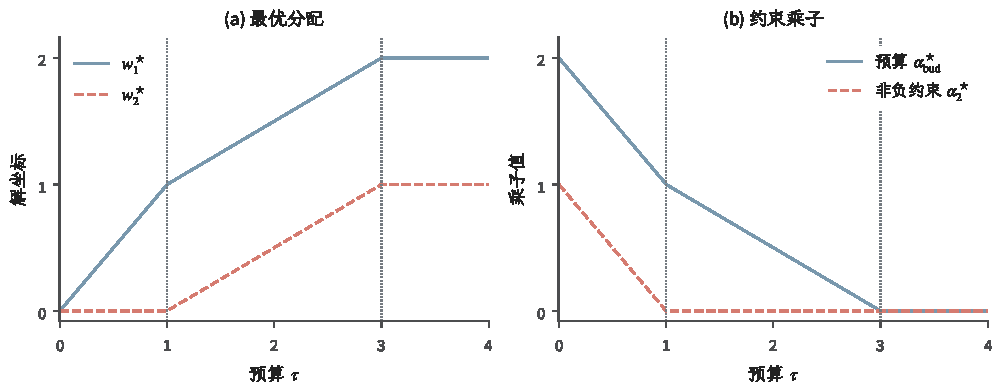
\includegraphics[width=\linewidth]{figures/math-preparation/concept-revision-analysis-functional/budget-active-set.pdf}
 \caption{例~\ref{ex:opt-kkt-budget}的解析解。左图为两个最优分配坐标，右图为预算乘子与第二个非负约束的乘子。竖参考线标出$\tau=1,3$；在切换点约束可以取等号而乘子为零，说明活跃性与正价格并不等价。}
 \label{fig:opt-budget-active-set}
\end{figure*}

一般地，设问题依赖参数$\tau$，活跃集在邻域内不变，把驻点条件、等式和活跃约束写成
$\bm{\Phi}(\bm{w},\bm{\nu},\bm{\alpha},\tau)=\bm{0}$。若对前三组变量的Jacobian
矩阵可逆，则第~\ref{chap:mathematical-analysis}章的隐式求导给出
\[
  \frac{d}{d\tau}
  \begin{bmatrix}\bm{w}^{\star}\\\bm{\nu}^{\star}\\\bm{\alpha}^{\star}\end{bmatrix}
  =
  -\left(\frac{\partial\bm{\Phi}}
  {\partial(\bm{w},\bm{\nu},\bm{\alpha})}\right)^{-1}
  \frac{\partial\bm{\Phi}}{\partial\tau}.
\]
这个Jacobian是完整KKT系统的导数，原目标Hessian可逆并不足以保证它可逆。活跃集改变或
该矩阵奇异时，解映射可能不可微；此时不能跨越切换点沿用同一个导数。

\subsection{原问题与对偶问题}
\label{sec:opt-duality}

\subsubsection{Lagrangian下界与弱对偶}

对固定乘子$\bm{\alpha}\geq\bm{0}$，任意可行$\bm{w}$都满足
$\mathcal{L}(\bm{w},\bm{\nu},\bm{\alpha})\leq f(\bm{w})$。因此
\term{对偶函数}（dual function）
\[
  q(\bm{\nu},\bm{\alpha})
  =\inf_{\bm{w}}\mathcal{L}(\bm{w},\bm{\nu},\bm{\alpha})
\]
给出原问题最优值的下界。最大化这个下界得到对偶问题。由构造立即有
$d^{\star}\leq p^{\star}$，称为\term{弱对偶}（weak duality）；差
$p^{\star}-d^{\star}$称为对偶间隙。对某组乘子取下确界得到$-\infty$，表示这组
乘子没有给出有限下界；对偶不可行则表示没有任何乘子满足对偶问题规定的可行条件。前者
描述一个候选乘子的函数值，后者描述整个候选集合，二者不能混用。

\subsubsection{Farkas择一与线性规划强对偶}

线性规划的强对偶可以从一个不可行证书推出。先建立所需的择一定理
\scite{math-boyd2004convex}

\begin{lemma}[有限生成锥的闭性]
\label{lem:opt-finitely-generated-cone}
给定$\bm{a}_1,\ldots,\bm{a}_r\in\mathbb{R}^m$，集合
\[
  K=\left\{\sum_{i=1}^r\alpha_i\bm{a}_i:\alpha_i\geq0\right\}
\]
是闭凸锥。
\end{lemma}

\begin{proof}
凸性和锥性质由非负线性组合直接得到。为证明闭性，先注意每个$\bm{x}\in K$都能由一组
线性无关的生成向量作非负组合。若某个表示使用的生成向量线性相关，就存在非零系数
$\bm{\gamma}$使$\sum_i\gamma_i\bm{a}_i=\bm{0}$；必要时改变符号，使至少一个
$\gamma_i>0$。从原系数中减去
$t\bm{\gamma}$，其中$t=\min_{\gamma_i>0}\alpha_i/\gamma_i$，仍保持所有系数
非负，并使至少一个系数变为零。重复此过程便得到线性无关的表示。

现取$\bm{x}^{(k)}\in K$且$\bm{x}^{(k)}\to\bm{x}$。线性无关的生成子集只有有限多个，
故可取子列，使每个$\bm{x}^{(k)}$都使用同一个子集$J$。以这些向量为列组成满列秩矩阵
$\bm{A}_J$，相应非负系数满足
\[
  \bm{\alpha}^{(k)}
  =(\bm{A}_J^{\top}\bm{A}_J)^{-1}\bm{A}_J^{\top}\bm{x}^{(k)}
  \longrightarrow
  (\bm{A}_J^{\top}\bm{A}_J)^{-1}\bm{A}_J^{\top}\bm{x}.
\]
极限系数仍逐项非负，且$\bm{x}$等于$\bm{A}_J$乘该极限系数，故$\bm{x}\in K$。
\end{proof}

\begin{lemma}[有限维多面体的线性像]
\label{lem:opt-polyhedral-image}
有限维多面体在线性映射下的像仍是多面体，因而是闭集。
\end{lemma}

\begin{proof}
设多面体$P=\{\bm{u}:\bm{B}\bm{u}\leq\bm{d}\}$，线性映射为
$\bm{v}=\bm{T}\bm{u}$。其图像
\[
  \{(\bm{u},\bm{v}):\bm{B}\bm{u}\leq\bm{d},\
  \bm{v}=\bm{T}\bm{u}\}
\]
是多面体，而$\bm{T}P$是该图像消去$\bm{u}$后的坐标投影。对一个待消变量，
Fourier--Motzkin消元分别收集其系数为正、为负和为零的不等式；每一对正、负系数
不等式消去该变量，零系数不等式原样保留。所得有限组非严格线性不等式恰好描述投影。
逐个消去$\bm{u}$的坐标，便得到$\bm{T}P$的有限线性不等式表示。多面体是有限个闭
半空间的交，因此闭。
\end{proof}

\begin{theorem}[Farkas择一定理]
\label{thm:opt-farkas}
给定$\bm{M}\in\mathbb{R}^{m\times d}$和$\bm{r}\in\mathbb{R}^m$，下列两个系统
恰有一个可行：
\[
  \bm{M}\bm{x}=\bm{r},\quad\bm{x}\geq\bm{0};
  \qquad
  \bm{M}^{\top}\bm{z}\geq\bm{0},\quad
  \bm{r}^{\top}\bm{z}<0.
\]
\end{theorem}

\begin{proof}
两者不能同时成立，因为若都成立，则
$0>\bm{r}^{\top}\bm{z}
=\bm{x}^{\top}\bm{M}^{\top}\bm{z}\geq0$，矛盾。
若第一个系统不可行，$\bm{r}$不属于锥
$K=\{\bm{M}\bm{x}:\bm{x}\geq\bm{0}\}$。它由$\bm{M}$的有限个列向量生成，故由
引理~\ref{lem:opt-finitely-generated-cone}可知$K$是闭凸锥。对$K$与$\bm{r}$应用
定理~\ref{thm:opt-projection-separation}，得到$\bm{a}$和$c$，使
$\langle\bm{a},\bm{k}\rangle\leq c<\langle\bm{a},\bm{r}\rangle$。
由于$\bm{0}\in K$，有$c\geq0$；又因为$t\bm{k}\in K$对所有$t\geq0$成立，
必有$\langle\bm{a},\bm{k}\rangle\leq0$，否则取充分大的$t$便会超过$c$。
令$\bm{z}=-\bm{a}$，可得$\langle\bm{z},\bm{r}\rangle<0$且
$\langle\bm{z},\bm{k}\rangle\geq0$对所有$\bm{k}\in K$成立。特别地，
对$\bm{M}$的每个列向量成立，故
$\bm{M}^{\top}\bm{z}\geq\bm{0}$。第二个系统可行。
\end{proof}

\begin{theorem}[有限维线性规划强对偶]
\label{thm:opt-lp-strong-duality}
考虑标准型原问题与对偶问题
\[
  \min_{\bm{x}\geq\bm{0}}\bm{c}^{\top}\bm{x}
  \quad\text{s.t.}\quad\bm{A}\bm{x}=\bm{b},
  \qquad
  \max_{\bm{y}}\bm{b}^{\top}\bm{y}
  \quad\text{s.t.}\quad\bm{A}^{\top}\bm{y}\leq\bm{c}.
\]
若原问题可行且有限下确界为$p^\star$，则原问题与对偶问题都有最优解，且两个最优值
都等于$p^\star$。
\end{theorem}

\begin{proof}
原始可行域
$P=\{\bm{x}:\bm{A}\bm{x}=\bm{b},\ \bm{x}\geq\bm{0}\}$是非空多面体。由
引理~\ref{lem:opt-polyhedral-image}，其目标值集合
\[
  W=\{\bm{c}^{\top}\bm{x}:\bm{x}\in P\}
\]
是$\mathbb{R}$中的非空多面体。集合$W$下有界，且一维多面体包含自己的有限下端点，
故$p^\star=\inf W$属于$W$。因此存在原始可行点$\bm{x}^{\star}$满足
$\bm{c}^{\top}\bm{x}^{\star}=p^\star$，原问题达到其最优值。

对任意$\varepsilon>0$，系统
\[
  \bm{A}\bm{x}=\bm{b},\quad
  \bm{c}^{\top}\bm{x}+s=p^\star-\varepsilon,\quad
  \bm{x}\geq\bm{0},\ s\geq0
\]
不可行，否则会有目标值小于$p^\star$的原始可行点。对增广矩阵应用
定理~\ref{thm:opt-farkas}，存在$(\bm{y}_{\varepsilon},\gamma_\varepsilon)$满足
\[
  \bm{A}^{\top}\bm{y}_{\varepsilon}
  +\gamma_\varepsilon\bm{c}\geq\bm{0},\quad
  \gamma_\varepsilon\geq0,\quad
  \bm{b}^{\top}\bm{y}_{\varepsilon}
  +\gamma_\varepsilon(p^\star-\varepsilon)<0.
\]
取任一原始可行$\bar{\bm{x}}$并与第一式作内积可知$\gamma_\varepsilon>0$，否则会与
最后一式矛盾。令
$\widehat{\bm{y}}_\varepsilon=-\bm{y}_\varepsilon/\gamma_\varepsilon$，便有
$\bm{A}^{\top}\widehat{\bm{y}}_\varepsilon\leq\bm{c}$且
$\bm{b}^{\top}\widehat{\bm{y}}_\varepsilon>p^\star-\varepsilon$。

记对偶可行多面体为
$D=\{\bm{y}:\bm{A}^{\top}\bm{y}\leq\bm{c}\}$。上面的构造说明$D$非空，且其
目标值集合
\[
  V=\{\bm{b}^{\top}\bm{y}:\bm{y}\in D\}
\]
对每个$\varepsilon>0$都包含一个大于$p^\star-\varepsilon$的值。弱对偶说明$V$中的
每个值都不超过$p^\star$，所以$\sup V=p^\star$。由
引理~\ref{lem:opt-polyhedral-image}，$V$是$\mathbb{R}$中的多面体；非空的一维
多面体只能是闭区间、闭射线、单点或整条实线。由于$V$有有限上确界，它必包含上端点
$p^\star$。因此存在$\bm{y}^{\star}\in D$使
$\bm{b}^{\top}\bm{y}^{\star}=p^\star$，对偶最优解达到与原问题相同的最优值。
\end{proof}

\begin{example}[二维资源分配的原始与对偶证书]
\label{ex:opt-resource-lp-duality}
考虑
\[
  \max_{x_1,x_2\geq0}3x_1+2x_2
  \quad\text{s.t.}\quad
  2x_1+x_2\leq4,\quad x_1+2x_2\leq4.
\]
为两类资源设置价格$u_1,u_2\geq0$。由于原问题是最大化，对可行点的资源余量按非负
价格计价会给出目标上界：
\begin{align*}
  \mathcal{L}(\bm{x},\bm{u})
  &=
  3x_1+2x_2
  +u_1(4-2x_1-x_2)+u_2(4-x_1-2x_2)\\
  &=
  4u_1+4u_2
  +(3-2u_1-u_2)x_1+(2-u_1-2u_2)x_2.
\end{align*}
要使$\sup_{\bm{x}\geq\bm{0}}\mathcal{L}(\bm{x},\bm{u})$有限，$x_1,x_2$的系数
必须非正，因而
$2u_1+u_2\geq3$且$u_1+2u_2\geq2$。此时上确界就是$4u_1+4u_2$，
最小化这个上界得到对偶
\[
  \min_{u_1,u_2\geq0}4u_1+4u_2
  \quad\text{s.t.}\quad
  2u_1+u_2\geq3,\quad u_1+2u_2\geq2.
\]
原始点$(x_1,x_2)=(4/3,4/3)$可行，值为$20/3$；对偶点
$(u_1,u_2)=(4/3,1/3)$可行，值也为$20/3$。弱对偶说明二者同时最优。两项资源约束
和两项产品约束均取等号，互补松弛也逐项成立。
\end{example}

\subsubsection{一般凸问题中的资格条件}

不可行、无界和未达到必须区分。Farkas向量证明约束不可行；若原问题沿可行射线无限改善，
弱对偶只说明不存在给出有限下界的对偶候选，也就是每个允许乘子的对偶函数值都为
$-\infty$，不能据此断言乘子候选集合为空。在线性规划标准型中，这种情形表现为对偶
不可行。若只有下确界而不达到，则不能展示原始最优点。一般凸问题在使用Slater条件前还需
处理低维定义域。沿用定义~\ref{def:opt-proper-domain-indicator}的有效定义域，还需说明低维集合中的“内部”。
\begin{definition}[仿射包与相对内部]
\label{def:opt-affine-hull-relative-interior}
对非空集合$C\subseteq\mathbb R^d$，其\term{仿射包}（affine hull）是全部有限仿射组合
$\sum_i\alpha_i\bm x_i$组成的集合，其中$\bm x_i\in C$、$\sum_i\alpha_i=1$，权重可为负。
点$\bm x\in C$属于\term{相对内部}（relative interior），是指存在$r>0$使
$B(\bm x,r)\cap\operatorname{aff}C\subseteq C$。
\end{definition}例如平面中的线段没有二维内部，但去掉两个端点后就是它的相对内部。

本章采用如下Slater版本。设$f$和不等式函数$g_k$都是适当凸函数，即它们不恒为
$+\infty$、从不取$-\infty$且至少在一点取有限值；这些函数具有共同凸定义域$D$，
等式约束为仿射约束$\bm{A}\bm{w}=\bm{b}$。若存在
\[
  \bar{\bm{w}}\in\operatorname{ri}D,\qquad
  \bm{A}\bar{\bm{w}}=\bm{b},\qquad
  g_k(\bar{\bm{w}})<0\quad\text{对所有 }k,
\]
并且原问题最优值有限，则原、对偶最优值相等，且存在最优对偶乘子。证明把可达到的
“约束余量—目标值”集合与严格低于原最优值的点分离；相对内部中的严格可行点排除了
目标系数为零的异常分离向量，归一化后便得到所需乘子。这里列出的定义域、仿射等式和
有限最优值都是所采用版本的一部分。凸性本身并不够，也不能把前面的线性规划证明原样
套到任意凸问题。第~\ref{chap:decision-theory-and-dynamic-risk}章会在状态、策略和
价值定义后，把同一对偶工具用于价值函数与占用度量。

\subsection{松弛与最优性证书}
\label{sec:opt-relaxations-certificates}

\subsubsection{凸包与可计算松弛}

第~\ref{chap:combinatorics}章已利用候选范围的包含关系建立松弛界。
现在还需区分两件事：连续集合能否精确包住原候选，以及返回的连续最优点能否恢复为原问题的解。
把原候选的加权平均一并纳入，可以得到包含这些候选的最小凸集。

\begin{definition}[有限点集的凸包]
\label{def:opt-convex-hull}
设$S=\{\bm s_1,\ldots,\bm s_N\}\subseteq\mathbb R^d$非空。
其凸包（convex hull）由这些点的全部凸组合构成：
\[
  \operatorname{conv}(S)
  =\left\{\sum_{i=1}^N\alpha_i\bm s_i:
  \alpha_i\geq0,\ \sum_{i=1}^N\alpha_i=1\right\}.
\]
\end{definition}
例如离散点集
\[
  S=\{(0,0),(1,0),(0,1)\}
\]
可以表示“至多选择一个项目”。把$S$替换为三角形
\[
  \operatorname{conv}(S)
  =\{(x_1,x_2):x_1,x_2\geq0,\ x_1+x_2\leq1\}
\]
得到\term{凸松弛}（convex relaxation）：原来的每个候选仍可行，但增加了分数候选。
对最小化问题，松弛最优值是原最优值的下界；对最大化问题则是上界。

对于有限非空$S$，精确凸包不改变任意线性目标$\bm{c}^{\top}\bm{x}$的最优值：任意
$\bm{x}=\sum_i\alpha_i\bm{s}_i\in\operatorname{conv}(S)$都满足
$\bm{c}^{\top}\bm{x}=\sum_i\alpha_i\bm{c}^{\top}\bm{s}_i
\geq\min_{\bm{s}\in S}\bm{c}^{\top}\bm{s}$，再结合
$S\subseteq\operatorname{conv}(S)$即得最小值相等，最大值同理。
数值相等仍没有指定求解器返回哪个点：若多个候选都最优，它们的凸组合也最优。

\begin{definition}[凸集的极点]
\label{def:opt-extreme-point}
设$K\subseteq\mathbb R^d$为凸集。若$\bm x\in K$满足：对任何$\bm u,\bm v\in K$
与$\theta\in(0,1)$，只要$\bm x=\theta\bm u+(1-\theta)\bm v$，就有
$\bm u=\bm v=\bm x$，则称$\bm x$为$K$的极点（extreme point）。
\end{definition}
极点不能再由其他可行点的非平凡平均得到。线性目标的所有最优点则组成同一个面。
\begin{definition}[线性目标的最优面]
\label{def:opt-optimal-face}
设线性目标$\bm c^\top\bm x$在非空凸集$K$上达到有限最大值$M$。
其最优面（optimal face）为
\[
  K^\star=\{\bm x\in K:\bm c^\top\bm x=M\}.
\]
最小化时，将$M$换为达到的有限最小值即可。
\end{definition}
当$K=\operatorname{conv}(S)$且$S$有限时，最优面正是$S$中全部最优点的凸包：
若一个凸组合对次优点给了正权重，其线性目标值便严格低于最大值。
若$S\subseteq\mathbb Z^d$，最优面还含有整数极点。可以在有限个整数最优点中，
按坐标次序逐项取最大值，选出一个点。若它是两个可行点的非平凡平均，线性最优性先迫使
这两个点都最优，再逐坐标的最大性迫使它们与所选点相同，因此该点确为极点。

即使如此，返回的最优点仍可能是分数点。例如上面的三角形在目标$x_1+x_2$下，
整条边$x_1+x_2=1$都是最优面，$(1/2,1/2)$也最优；逐坐标向上取整却得到
不属于原点集的$(1,1)$。整数极点的存在不保证任意分数最优点都能直接取整。

精确凸包的完整不等式描述可能难以获得。只保留局部约束通常
得到更大的多面体，计算较容易而界更松。也可以把乘积$x_ix_j$提升为矩阵变量并要求某个
块矩阵半正定，得到半正定松弛；它利用二次一致性，代价是矩阵锥约束更昂贵。

\subsubsection{上下界与最优性证书}

取整还可能破坏约束。考虑
\[
  \max_{x_1,x_2\in\{0,1\}}x_1+x_2
  \quad\text{s.t.}\quad 2x_1+2x_2\leq3.
\]
整数最优值为$1$，而把变量放宽到$[0,1]$后，$(3/4,3/4)$可行且目标值为$3/2$。
逐坐标四舍五入得到$(1,1)$，却违反容量约束；逐坐标向下取整虽可行，却得到目标值$0$。
因此松弛值、恢复可行性的规则和恢复后的目标损失必须分别分析。

若松弛集合比整数可行点的凸包更大，松弛最优值可能严格优于所有整数可行解；
这种最优值差异称为\term{整数间隙}（integrality gap）。上例采用加法差距时，间隙为
$3/2-1=1/2$。更大的松弛不一定产生严格间隙，它还取决于目标；
精确凸包对线性目标没有这种最优值差异，却仍可能包含分数最优点。

图~\ref{fig:opt-hull-relaxation}固定同一个整数问题，把两种连续可行域并列。
精确凸包上的最优值与整数候选一致；局部容量约束定义的松弛多出了整数候选无法平均
得到的区域。这一多出的区域，才使目标上界从$1$升到$3/2$。
\begin{figure*}[htbp]
 \centering
 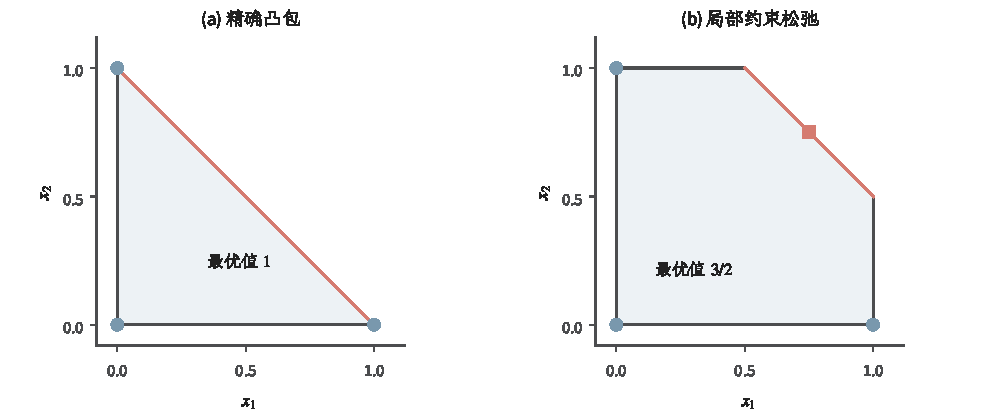
\includegraphics[width=\linewidth]{figures/math-preparation/concept-revision-analysis-functional/hull-relaxation.pdf}
 \caption{最大化$x_1+x_2$的两种放宽。左图精确凸包满足$x_1+x_2\leq1$；右图局部松弛满足$0\leq x_i\leq1$与$x_1+x_2\leq3/2$。实心圆为整数可行点，方形为右图的分数最优点$(3/4,3/4)$，粗边标出各自最优面。两图采用相同坐标尺度。}
 \label{fig:opt-hull-relaxation}
\end{figure*}

集合函数的连续扩展也有多种选择。连续变量上的凸性或凹性必须针对所选扩展检验，
不能仅凭原集合函数次模就断言成立；扩展方式决定可用的优化工具。
第~\ref{chap:graph-theory}章会讨论一个可精确求解的特殊情形：二值成对能量满足相应
次模不等式时，可以表示为非负容量的割。一般集合函数的次模性本身，并不保证任意
次模最大化或最小化都能用图割解决。

可计算界构成停止证书。对最小化问题，若可行解给出上界$U$，对偶或松弛给出下界$L$，
则
\[
  0\leq U-p^\star\leq U-L.
\]
当$U=L$时已证明全局最优。若把松弛解取整为可行解$\widehat{\bm{x}}$，还应单独分析
$f(\widehat{\bm{x}})-L$；“取整后看起来接近”不是误差界。互补松弛能够证明哪些约束在
最优点活跃，却不总能直接构造整数解。图模型中的边缘多面体和MAP松弛会在图与概率对象
建立后复用这里的凸包、上下界和间隙概念。

\section{光滑目标的迭代求解}
\label{sec:opt-smooth-iterative-methods}

有了可判定的最优性条件，还需构造能逐步接近它的参数序列。这里先限定目标可微且梯度光滑：
梯度下降用一阶信息保证单步改善，动量和预条件再利用迭代历史或曲率改变移动方向。
每种改进的保证都应与前节的曲率条件配对，而不能仅凭更新公式判断快慢。

\subsection{梯度下降与步长}
\label{sec:opt-gradient-descent}

\subsubsection{光滑上界与单步下降}

梯度给出最陡的一阶下降方向，但一步走多远取决于函数弯曲程度。光滑性把局部线性近似的
余项控制为二次量\scite{math-nocedal2006numerical}。本小节考虑可微函数
$f:\mathbb R^d\to\mathbb R$，并选取一个正的梯度Lipschitz上界$L>0$。
若梯度恒定，仍可选择任意正上界；这样后面的$1/L$步长也有定义。
全空间的设定保证更新点仍在函数定义域内；若目标只定义在开凸子域上，使用下降引理时
还须确认两端点及其线段留在该域内，不能直接把任意梯度步代入。

\begin{lemma}[下降引理]
\label{lem:opt-descent}
若$f:\mathbb R^d\to\mathbb R$可微且梯度是$L$-Lipschitz连续的，$L>0$，则对任意
$\bm u,\bm v\in\mathbb R^d$，
\begin{equation}
  f(\bm{v})\leq f(\bm{u})
  +\langle\nabla f(\bm{u}),\bm{v}-\bm{u}\rangle
  +\frac{L}{2}\lVert\bm{v}-\bm{u}\rVert_2^2.
  \label{eq:opt-descent-lemma}
\end{equation}
\end{lemma}

\begin{proof}
令$\bm{d}=\bm{v}-\bm{u}$。沿线段积分并减去一阶项可得
\[
  f(\bm{v})-f(\bm{u})-\langle\nabla f(\bm{u}),\bm{d}\rangle
  =
  \int_0^1
  \langle\nabla f(\bm{u}+t\bm{d})-\nabla f(\bm{u}),\bm{d}\rangle\,dt.
\]
由Cauchy--Schwarz不等式和梯度Lipschitz条件，被积函数至多为
$Lt\lVert\bm{d}\rVert_2^2$；积分即得结论。
\end{proof}

梯度下降按
\begin{equation}
  \bm{w}^{(t+1)}
  =\bm{w}^{(t)}-\eta\nabla f(\bm{w}^{(t)})
  \label{eq:opt-gradient-descent}
\end{equation}
更新。把$\bm{v}$取为右端点代入下降引理，得到
\begin{equation}
  f(\bm{w}^{(t+1)})
  \leq f(\bm{w}^{(t)})
  -\eta\left(1-\frac{L\eta}{2}\right)
  \lVert\nabla f(\bm{w}^{(t)})\rVert_2^2.
  \label{eq:opt-gradient-single-step}
\end{equation}
所以$0<\eta<2/L$保证每个非驻点处严格下降。若$f$下有界，记其有限下确界为
\[
  f_{\inf}:=\inf_{\bm{w}\in\mathbb{R}^d}f(\bm{w})>-\infty.
\]
取$\eta=1/L$并对$t=0,\ldots,T-1$求和，可得非凸光滑情形的保证
\begin{equation}
  \min_{0\leq t<T}\lVert\nabla f(\bm{w}^{(t)})\rVert_2^2
  \leq
  \frac{2L(f(\bm{w}^{(0)})-f_{\inf})}{T}.
  \label{eq:opt-nonconvex-gradient-rate}
\end{equation}
它只说明某次迭代接近驻点，没有声称驻点是全局最优点。

步长上界在一维二次函数上即可看到。对$f(w)=Lw^2/2$，
$w^{(t+1)}=(1-\eta L)w^{(t)}$。当$\eta=2/L$时迭代在正负之间等幅振荡；
$\eta>2/L$时幅度按$|1-\eta L|>1$增长。负梯度方向本身没有错，失败来自步长跨过了
曲率允许的稳定范围。

\subsubsection{不同曲率下的收敛证明}

若$f$还凸、最小点$\bm{w}^{\star}$存在，并继续取$\eta=1/L$，则由凸性有
$f(\bm{w}^{(t)})-f^\star
\leq\langle\nabla f(\bm{w}^{(t)}),\bm{w}^{(t)}-\bm{w}^{\star}\rangle$。
先展开距离平方并使用这个不等式：
\begin{align*}
  \lVert\bm{w}^{(t+1)}-\bm{w}^{\star}\rVert_2^2
  &=
  \lVert\bm{w}^{(t)}-\bm{w}^{\star}\rVert_2^2
  -\frac{2}{L}
  \left\langle\nabla f(\bm{w}^{(t)}),
  \bm{w}^{(t)}-\bm{w}^{\star}\right\rangle\\
  &\qquad
  +\frac{1}{L^2}\lVert\nabla f(\bm{w}^{(t)})\rVert_2^2\\
  &\leq
  \lVert\bm{w}^{(t)}-\bm{w}^{\star}\rVert_2^2
  -\frac{2}{L}\bigl(f(\bm{w}^{(t)})-f^\star\bigr)\\
  &\qquad
  +\frac{1}{L^2}\lVert\nabla f(\bm{w}^{(t)})\rVert_2^2.
\end{align*}
另一方面，把$\eta=1/L$代入式~\eqref{eq:opt-gradient-single-step}可得
\[
  \frac{1}{L^2}\lVert\nabla f(\bm{w}^{(t)})\rVert_2^2
  \leq
  \frac{2}{L}\bigl(
  f(\bm{w}^{(t)})-f(\bm{w}^{(t+1)})\bigr).
\]
用后一式消去梯度平方项，得到
\[
  \lVert\bm{w}^{(t+1)}-\bm{w}^{\star}\rVert_2^2
  \leq
  \lVert\bm{w}^{(t)}-\bm{w}^{\star}\rVert_2^2
  -\frac{2}{L}\bigl(f(\bm{w}^{(t+1)})-f^\star\bigr).
\]
对$t=0,\ldots,T-1$求和并去掉末端的非负距离，便有
\[
  \frac{2}{L}\sum_{t=0}^{T-1}
  \bigl(f(\bm{w}^{(t+1)})-f^\star\bigr)
  \leq
  \lVert\bm{w}^{(0)}-\bm{w}^{\star}\rVert_2^2.
\]
式~\eqref{eq:opt-gradient-single-step}还说明目标值单调不增，因此左侧求和中的每一项
都不小于$f(\bm{w}^{(T)})-f^\star$。于是
\begin{equation}
  f(\bm{w}^{(T)})-f^\star
  \leq\frac{L\lVert\bm{w}^{(0)}-\bm{w}^{\star}\rVert_2^2}{2T}.
  \label{eq:opt-convex-gradient-rate}
\end{equation}

若满足PL条件，把式~\eqref{eq:opt-pl-condition}代入
式~\eqref{eq:opt-gradient-single-step}，在$\eta=1/L$时得到
\begin{equation}
  f(\bm{w}^{(t)})-f^\star
  \leq
  \left(1-\frac{\mu}{L}\right)^t
  \bigl(f(\bm{w}^{(0)})-f^\star\bigr).
  \label{eq:opt-pl-linear-rate}
\end{equation}
强凸函数满足PL条件，还由
$f(\bm{w})-f^\star\geq\mu\lVert\bm{w}-\bm{w}^{\star}\rVert_2^2/2$
把目标误差转成参数误差。没有强凸时，式~\eqref{eq:opt-pl-linear-rate}不保证迭代趋向
某个唯一参数。

固定步长需要已知或估计$L$。回溯线搜索从候选步长开始缩小，直到
$f(\bm{w}-\eta\nabla f(\bm{w}))\leq
f(\bm{w})-c\eta\lVert\nabla f(\bm{w})\rVert_2^2$成立，其中$c\in(0,1)$。
学习率调度则预先或按进度改变$\eta_t$。线搜索用实际函数值核验当前一步，调度只规定时间
表；二者都不能弥补错误梯度或无下界目标。

\subsection{代理上界与单调改善}
\label{sec:opt-majorization-improvement}

梯度下降利用一个可计算二次上界。若上界来自别的可解结构，同一下降逻辑也能使用，
而不要求变量分块或目标本身是二次函数。
\begin{definition}[主化代理与MM更新]
\label{def:opt-majorization-minimization}
给定目标$F:C\to\mathbb R$、当前点$\bm w^{(t)}\in C$，
\term{主化--最小化方法}（majorization--minimization, MM）在当前点
$\bm{w}^{(t)}$构造代理函数$Q(\bm{w}\mid\bm{w}^{(t)})$，满足
\[
  F(\bm{w})\leq Q(\bm{w}\mid\bm{w}^{(t)}),
  \qquad
  F(\bm{w}^{(t)})=Q(\bm{w}^{(t)}\mid\bm{w}^{(t)}).
\]
上界关系要求对所有$\bm w\in C$成立。若新点$\bm w^{(t+1)}\in C$满足代理值不增，
就称这一步为MM改善更新。
\end{definition}
此时
\begin{align*}
  F(\bm{w}^{(t+1)})
  &\leq Q(\bm{w}^{(t+1)}\mid\bm{w}^{(t)})\\
  &\leq Q(\bm{w}^{(t)}\mid\bm{w}^{(t)})
  =F(\bm{w}^{(t)}).
\end{align*}
第一步用全局上界，第二步用代理改善，最后一步用切触条件。若代理只在当前点附近控制原
目标，而新点走出该邻域，单调链条便会断裂。

下降引理本身给出一个显式代理。若$F$为$L$光滑，可取
\[
  Q(\bm{w}\mid\bm{w}^{(t)})
  =F(\bm{w}^{(t)})
  +\langle\nabla F(\bm{w}^{(t)}),\bm{w}-\bm{w}^{(t)}\rangle
  +\frac{L}{2}\lVert\bm{w}-\bm{w}^{(t)}\rVert_2^2.
\]
它在当前点切触并全局上界$F$；精确最小化$Q$恰好得到步长$1/L$的梯度更新。仅让代理
与原目标在当前点具有相同梯度，却不满足全局上界，不能推出上面的单调不等式链。

例如$F(x)=x^2/2$、当前点$x^{(t)}=1$，取
$Q(x\mid1)=1/2+(x-1)+(x-1)^2$，则$Q-F=(x-1)^2/2\geq0$且当前点取等号。
代理最小点为$1/2$，于是$F(1/2)=1/8\leq Q(1/2\mid1)=1/4\leq F(1)=1/2$。
图~\ref{fig:opt-majorizer-versus-tangent}把这条链与只有相同局部斜率的切线对照。
\begin{figure}[htbp]
 \centering
 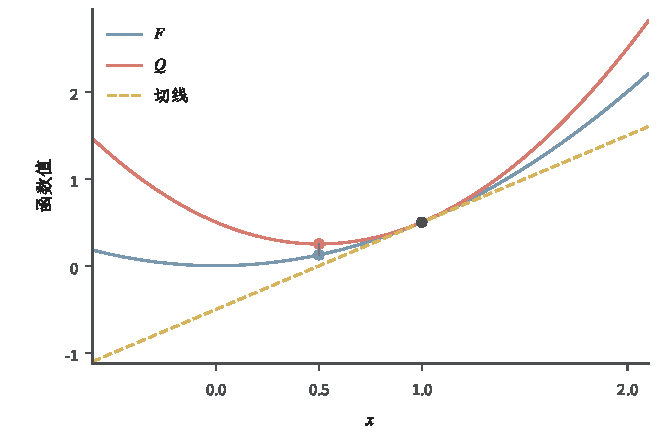
\includegraphics[width=\linewidth]{figures/math-preparation/reader-revision-analysis/optimization-majorizer-versus-tangent.pdf}
 \caption{代理上界与切线的区别。蓝线为$F(x)=x^2/2$，红线为当前点$1$处的主化代理$Q$，
 黄虚线为同点切线$x-1/2$。三者在当前点同值同斜率，但切线位于目标下方，
 最小化它不能使用MM的上界链；红点标出代理最小点对应的值。图为解析教学示例。}
 \label{fig:opt-majorizer-versus-tangent}
\end{figure}

\subsection{曲率、加速与预条件}
\label{sec:opt-curvature-acceleration}

梯度下降的收敛界已经显示，方向上的曲率差异会限制统一步长。
加速递推利用迭代历史，预条件则改变不同方向的尺度；牛顿法进一步用局部二阶近似。
这三种机制改变不同部分，条件与收益须分别对照，不能由一个二阶矩阵的出现就认定获得加速。

\subsubsection{动量与加速的递推结构}

对二次函数$f(\bm{w})=\frac12\bm{w}^{\top}\bm{H}\bm{w}
-\bm{c}^{\top}\bm{w}$，梯度下降的误差满足
$\bm{e}^{(t+1)}=(\bm{I}-\eta\bm{H})\bm{e}^{(t)}$。当
$\bm{H}\succ\bm{0}$但条件数$\kappa=L/\mu$很大时，同一步长必须同时照顾陡峭与平坦
方向，平坦方向因而收敛缓慢。

\term{动量法}（momentum method）保存过去方向：
\[
  \bm{v}^{(t+1)}=\beta\bm{v}^{(t)}+\nabla f(\bm{w}^{(t)}),
  \qquad
  \bm{w}^{(t+1)}=\bm{w}^{(t)}-\eta\bm{v}^{(t+1)}.
\]
它通过二阶递推重塑各特征方向上的多项式响应，但$\beta$和$\eta$不能各自独立地任取。
对上述正定二次目标，曲率为$\lambda_i$的特征方向满足
\[
  e_i^{(t+1)}
  =(1+\beta-\eta\lambda_i)e_i^{(t)}-\beta e_i^{(t-1)}.
\]
该方向的两个特征根都严格位于单位圆内，当且仅当
$-1<\beta<1$且$0<\eta\lambda_i<2(1+\beta)$。因而常用的
$0\leq\beta<1$还须配合$0<\eta<2(1+\beta)/L$，才能保证所有方向稳定。
若已知$0<\mu\leq\lambda_i\leq L$，经典重球参数
\[
  \eta=\frac{4}{(\sqrt{L}+\sqrt{\mu})^2},
  \qquad
  \beta=\left(\frac{\sqrt{L}-\sqrt{\mu}}
  {\sqrt{L}+\sqrt{\mu}}\right)^2
\]
给出这一二次模型上的代表性最坏方向速率；它不是一般非凸目标或含噪梯度下的无条件
调参规则。

\term{Nesterov加速梯度}
（Nesterov accelerated gradient）在前瞻点计算梯度：
\[
  \bm{z}^{(t)}=\bm{w}^{(t)}+\beta_t(\bm{w}^{(t)}-\bm{w}^{(t-1)}),
  \qquad
  \bm{w}^{(t+1)}=\bm{z}^{(t)}-\frac1L\nabla f(\bm{z}^{(t)}).
\]
令$\bm{w}^{(-1)}=\bm{w}^{(0)}$、$q_0=1$，并取
\[
  q_{t+1}=\frac{1+\sqrt{1+4q_t^2}}{2},
  \qquad
  \beta_t=\frac{q_t-1}{q_{t+1}}.
\]
若$f$为凸可微函数、梯度$L$-Lipschitz连续、最小点存在，并且每步使用精确梯度和
步长$1/L$，则上述选择给出
$f(\bm{w}^{(t)})-f^\star=O(1/t^2)$；同样条件下，普通梯度下降的一般保证为
$O(1/t)$。强凸时还可采用依赖$\mu/L$的固定系数得到线性速率，但那是另一组参数和证明。
在一维二次函数$f(w)=\lambda w^2/2$上，这个迭代可直接核验为
\[
  w^{(t+1)}
  =\left(1-\frac{\lambda}{L}\right)
  \bigl((1+\beta_t)w^{(t)}-\beta_t w^{(t-1)}\bigr).
\]
当$\lambda=L$时一步到达零点；当$\lambda\ll L$时，跨步项改变平坦方向上的二阶递推，
但系数选错仍会振荡。一般凸证明不能只检查这个二次算例，而是构造同时含目标误差与外推
距离的势函数；$q_{t+1}^2-q_{t+1}=q_t^2$使相邻两步的耦合项抵消，最终留下
$q_t^2(f(\bm{w}^{(t)})-f^\star)$的统一上界。加速结论因此来自特定外推序列与势函数
不等式，不能由“加入惯性”本身推出。

\subsubsection{牛顿法、近似曲率与预条件}

\term{牛顿法}（Newton's method）在$\bm{w}^{(t)}$处使用关于增量$\bm{p}$的局部
二次模型
\[
  m_t(\bm{p})
  =
  f(\bm{w}^{(t)})
  +\left\langle\nabla f(\bm{w}^{(t)}),\bm{p}\right\rangle
  +\frac12\bm{p}^{\top}\nabla^2f(\bm{w}^{(t)})\bm{p}.
\]
令$\nabla_{\bm{p}}m_t(\bm{p}^{(t)})=\bm{0}$，便得到牛顿方程
\[
  \nabla^2 f(\bm{w}^{(t)})\bm{p}^{(t)}
  =-\nabla f(\bm{w}^{(t)}),\qquad
  \bm{w}^{(t+1)}=\bm{w}^{(t)}+\alpha_t\bm{p}^{(t)}.
\]
若Hessian矩阵在最优点附近正定且Lipschitz连续，取单位步长可得到局部二次收敛。但Hessian矩阵
不定时，牛顿方向未必下降；离最优点较远时还需线搜索或信赖域。

对非线性最小二乘
$f(\bm{w})=\frac12\lVert\bm{r}(\bm{w})\rVert_2^2$，设
$\bm{r}:\mathbb{R}^d\to\mathbb{R}^m$。记残差向量的Jacobian矩阵为
$\bm{J}(\bm{w})\in\mathbb{R}^{m\times d}$，其第$i$行为
$\bm{J}_{i,:}(\bm{w})=\nabla r_i(\bm{w})^{\top}$，则
\[
  \nabla^2f(\bm{w})
  =\bm{J}(\bm{w})^{\top}\bm{J}(\bm{w})
  +\sum_{i=1}^m r_i(\bm{w})\nabla^2r_i(\bm{w}).
\]
\term{Gauss--Newton法}忽略第二项，使用半正定矩阵
$\bm{J}^{\top}\bm{J}$。当残差小或残差函数近似线性时近似合理；残差大时，省略项可能
决定曲率。

\term{拟牛顿法}（quasi-Newton method）不显式计算Hessian矩阵，而用梯度差
$\bm{y}^{(t)}=\nabla f(\bm{w}^{(t+1)})-\nabla f(\bm{w}^{(t)})$和步长
$\bm{s}^{(t)}=\bm{w}^{(t+1)}-\bm{w}^{(t)}$更新矩阵近似，并满足割线条件
$\bm{B}^{(t+1)}\bm{s}^{(t)}=\bm{y}^{(t)}$。若$\bm{B}^{(t)}$近似Hessian矩阵，
BFGS更新为
\begin{equation}
  \bm{B}^{(t+1)}
  =
  \bm{B}^{(t)}
  +
  \frac{\bm{y}^{(t)}(\bm{y}^{(t)})^{\top}}
       {(\bm{y}^{(t)})^{\top}\bm{s}^{(t)}}
  -
  \frac{\bm{B}^{(t)}\bm{s}^{(t)}(\bm{s}^{(t)})^{\top}\bm{B}^{(t)}}
       {(\bm{s}^{(t)})^{\top}\bm{B}^{(t)}\bm{s}^{(t)}}.
  \label{eq:opt-bfgs-update}
\end{equation}
当$\bm{B}^{(t)}\succ\bm{0}$且曲率条件
$(\bm{y}^{(t)})^{\top}\bm{s}^{(t)}>0$成立时，
式~\eqref{eq:opt-bfgs-update}保持$\bm{B}^{(t+1)}\succ\bm{0}$，相应搜索方向
$-(\bm{B}^{(t+1)})^{-1}\nabla f$才由正定性保证是下降方向。沿下降方向执行满足
Wolfe条件的线搜索可产生该正曲率内积。具体地，令
$\bm{w}^{(t+1)}=\bm{w}^{(t)}+\alpha_t\bm{p}^{(t)}$，其中
$\nabla f(\bm{w}^{(t)})^{\top}\bm{p}^{(t)}<0$。Wolfe条件要求存在
$0<c_1<c_2<1$使
\begin{equation}
\begin{aligned}
  f(\bm{w}^{(t+1)})
  &\leq
  f(\bm{w}^{(t)})
  +
  c_1\alpha_t
  \nabla f(\bm{w}^{(t)})^{\top}\bm{p}^{(t)},\\
  \nabla f(\bm{w}^{(t+1)})^{\top}\bm{p}^{(t)}
  &\geq
  c_2\nabla f(\bm{w}^{(t)})^{\top}\bm{p}^{(t)}.
\end{aligned}
\label{eq:opt-wolfe-conditions}
\end{equation}
第二行就是\term{Wolfe曲率条件}（Wolfe curvature condition）。由
$\bm{s}^{(t)}=\alpha_t\bm{p}^{(t)}$可得
\[
  (\bm{y}^{(t)})^{\top}\bm{s}^{(t)}
  \geq
  \alpha_t(c_2-1)
  \nabla f(\bm{w}^{(t)})^{\top}\bm{p}^{(t)}
  >0.
\]
非凸或梯度含噪时，上述条件可能难以满足，此时可能需要阻尼或跳过更新。

\term{预条件}（preconditioning）则选择正定矩阵$\bm{P}$，按
\[
  \bm{w}^{(t+1)}
  =
  \bm{w}^{(t)}-\eta\bm{P}\nabla f(\bm{w}^{(t)})
\]
更新。
这等价于在新的坐标或内积下做最陡下降。若\(p_i>0\)，并且
\[
  \bm{P}
  =
  \bm{Q}\operatorname{diag}(p_1,\ldots,p_d)\bm{Q}^{\top},
\]
则定义
\[
  \bm{P}^{1/2}
  =
  \bm{Q}\operatorname{diag}(\sqrt{p_1},\ldots,\sqrt{p_d})\bm{Q}^{\top}.
\]
这就是$\bm{P}$唯一的对称正定平方根：它满足
$\bm{P}^{1/2}\bm{P}^{1/2}=\bm{P}$，并且可逆，其逆记为$\bm{P}^{-1/2}$。
对当前正定二次目标，记
\[
  \widetilde{\bm{H}}=\bm{P}^{1/2}\bm{H}\bm{P}^{1/2},
  \qquad
  0<\widetilde{\mu}
  =\lambda_{\min}(\widetilde{\bm{H}})
  \leq\lambda_{\max}(\widetilde{\bm{H}})
  =\widetilde{L}.
\]
原坐标中的误差递推为
$\bm{e}^{(t+1)}=(\bm{I}-\eta\bm{P}\bm{H})\bm{e}^{(t)}$。令
$\widetilde{\bm{e}}^{(t)}=\bm{P}^{-1/2}\bm{e}^{(t)}$，则
\[
  \widetilde{\bm{e}}^{(t+1)}
  =
  (\bm{I}-\eta\widetilde{\bm{H}})
  \widetilde{\bm{e}}^{(t)},
  \qquad
  \bm{P}^{-1/2}
  (\bm{I}-\eta\bm{P}\bm{H})
  \bm{P}^{1/2}
  =
  \bm{I}-\eta\widetilde{\bm{H}}.
\]
右侧矩阵由可逆坐标变换$\bm{P}^{1/2}$得到，因而与原误差递推矩阵相似；相似矩阵具有
相同特征值。由于$\widetilde{\bm{H}}$对称正定，迭代对任意初始误差收敛当且仅当
$0<\eta<2/\widetilde{L}$。取
$\eta=2/(\widetilde{L}+\widetilde{\mu})$时，在变换后的欧氏范数中，每步最坏收缩因子为
\[
  \frac{\widetilde{\kappa}-1}{\widetilde{\kappa}+1},
  \qquad
  \widetilde{\kappa}
  =\frac{\widetilde{L}}{\widetilde{\mu}}.
\]
因此预条件的目标不是单独让$\bm{P}$的条件数小，而是让变换后曲率
$\widetilde{\bm{H}}$的条件数接近$1$。固定$\bm{P}\succ\bm{0}$只保证定义了合法内积；
若它与$\bm{H}$不匹配，$\widetilde{\kappa}$反而可能增大。对一般二阶可微的光滑强凸
函数，需要在所有迭代经过的区域统一满足
$\widetilde{\mu}\bm{I}\preceq
\bm{P}^{1/2}\nabla^2f(\bm{w})\bm{P}^{1/2}
\preceq\widetilde{L}\bm{I}$，上述步长范围与线性收敛解释才相应延续；变化的预条件矩阵还需
额外控制。

动量利用历史更新，牛顿类近似当前曲率，预条件改变几何尺度；三者可能组合，却不是同一种
机制。第~\ref{chap:matrix-analysis}章将在矩阵函数与Kronecker结构建立后给出结构化
预条件，Fisher矩阵与经验梯度二阶矩的差别则需等概率对象建立后讨论。

\begin{example}[两个曲率方向上的预条件]
\label{ex:opt-anisotropic-preconditioning}
取$f(\bm w)=(w_1^2+16w_2^2)/2$，初值$(2,2)^{\top}$。普通梯度下降若取
$\eta=0.1$，两个坐标分别乘以$0.9$与$-0.6$，因而
$\bm w^{(t)}=(2\times0.9^t,\,2\times(-0.6)^t)^{\top}$。
第二坐标来回越过谷底，第一坐标却缓慢缩小。取
$\bm P=\operatorname{diag}(1,1/16)$及$\eta=1/2$后，
$\bm P\nabla f(\bm w)=\bm w$，两坐标每步都减半。
\end{example}

\begin{figure*}[htbp]
 \centering
 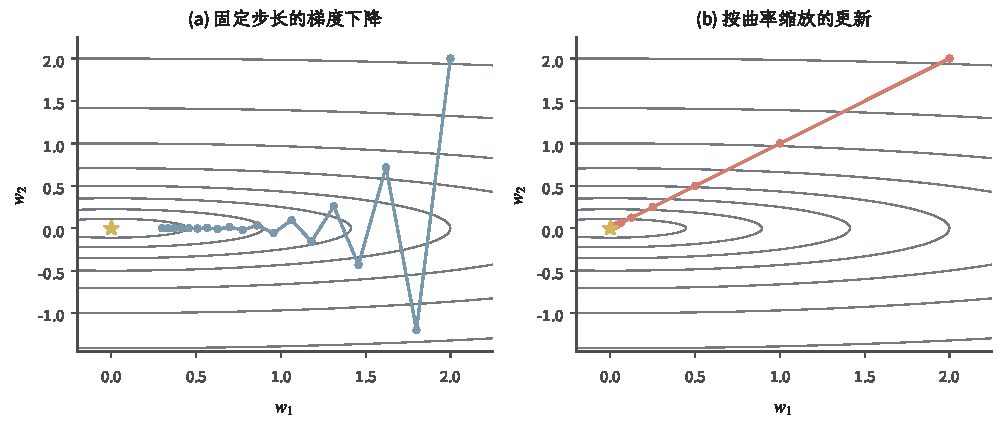
\includegraphics[width=\linewidth]{figures/math-preparation/analysis-geometry/optimization-preconditioned-paths.pdf}
 \caption{例~\ref{ex:opt-anisotropic-preconditioning}中的精确更新路径。灰线是同一二次目标的等值线，蓝、红圆点分别表示普通更新与预条件更新，黄色星号是最小点。预条件使用了已知曲率，获得和应用这一矩阵的成本仍属于算法代价。}
 \label{fig:opt-preconditioned-paths}
\end{figure*}

这个例子中的预条件恰好消除了两个方向的尺度差。一般目标的曲率会随位置变化，近似矩阵
也有误差；因此图中的直达路径解释机制，不构成所有预条件方法都更快的保证。

\section{非光滑与随机目标的求解}
\label{sec:opt-nonsmooth-stochastic-methods}

接下来改变的是算法能取得的局部信息。绝对值等正则项使普通梯度不存在，
大规模数据又可能只允许计算带噪声的梯度估计。非光滑性和随机性是两种不同障碍：
前者需要次梯度或邻近映射，后者需要控制误差积累；两者可以出现在同一个问题中。

\subsection{非光滑目标与正则化}
\label{sec:opt-nonsmooth-proximal}

\subsubsection{次梯度与非光滑最优性}

绝对值损失和$\ell_1$稀疏惩罚在零点不可微，但凸函数仍可用支撑直线描述。
\begin{definition}[凸次梯度与次微分]
\label{def:opt-convex-subgradient}
设$f:\mathbb R^d\to\mathbb R\cup\{+\infty\}$为适当凸函数，$f(\bm u)$有限。
向量$\bm{g}\in\mathbb R^d$若满足
\[
  f(\bm{v})\geq f(\bm{u})+\langle\bm{g},\bm{v}-\bm{u}\rangle
  \quad\text{对所有 }\bm{v},
\]
就称为$f$在$\bm{u}$处的\term{次梯度}（subgradient）。全部次梯度组成
$\partial f(\bm{u})$，称为次微分；它可以是空集。
\end{definition}
例如
\[
  \partial |x|=
  \begin{cases}
    \{1\},&x>0,\\
    [-1,1],&x=0,\\
    \{-1\},&x<0.
  \end{cases}
\]
凸函数在$\bm{w}^{\star}$处最优，当且仅当
$\bm{0}\in\partial f(\bm{w}^{\star})$。若零向量是次梯度，定义立即给出
$f(\bm{v})\geq f(\bm{w}^{\star})$；反过来，若$\bm{w}^{\star}$全局最优，则
$f(\bm{v})\geq f(\bm{w}^{\star})+\langle\bm{0},\bm{v}-\bm{w}^{\star}\rangle$，
所以零向量满足次梯度定义。这个等价性依赖凸次梯度采用全局下界定义。
若要把$f+r$的次微分直接写成$\partial f+\partial r$，或把约束写成指标函数后拆分
次微分，还需共同相对内部等相应资格条件；不能只凭两个函数都凸就无条件使用求和等式。

\subsubsection{投影、邻近与软阈值}

对闭凸集$C$，欧氏\term{投影}（projection）
$\Pi_C(\bm{z})=\argmin_{\bm{w}\in C}\lVert\bm{w}-\bm{z}\rVert_2^2$
把一步梯度更新拉回可行域：
\[
  \bm{w}^{(t+1)}
  =\Pi_C\bigl(\bm{w}^{(t)}-\eta_t\nabla f(\bm{w}^{(t)})\bigr).
\]
定理~\ref{thm:opt-projection-separation}的证明已经说明，在有限维空间中，非空闭性保证
最近点存在，而凸性与平方距离的严格凸性共同保证唯一。若$C$非凸，最近点可能不唯一。

投影处理一个硬可行域；若希望保留整个空间中的候选，却对不同候选收取不同惩罚，
就要在“惩罚小”和“离当前点近”之间取得平衡。
\begin{definition}[凸函数的邻近算子]
\label{def:opt-proximal-operator}
设$r:\mathbb R^d\to\mathbb R\cup\{+\infty\}$适当、下半连续且凸，$\eta>0$。
函数$r$的\term{邻近算子}（proximal operator）定义为
\[
  \operatorname{prox}_{\eta r}(\bm{z})
  =\argmin_{\bm{w}}
  \left\{r(\bm{w})+\frac{1}{2\eta}
  \lVert\bm{w}-\bm{z}\rVert_2^2\right\}.
\]
\end{definition}
这里的$\eta$调节惩罚与距离的相对权重；它还未指代某个算法的迭代步数。二次项使目标强凸。
适当闭凸函数具有仿射下界，二次项在无穷远处超过这个下界的线性下降，所以子问题强制；
强制性与下半连续性保证最小点存在，强凸性保证它唯一，所以邻近算子对每个$\bm{z}$都有
单值输出。
指标函数$\iota_C$在$C$上为零、在外部为$+\infty$，其邻近算子正是投影。
对$f+r$，近端梯度先按光滑部分$f$走一步，再用$r$的邻近算子处理非光滑结构。

\begin{theorem}[$\ell_1$邻近算子是软阈值]
\label{thm:opt-soft-threshold}
设$\lambda\geq0$、$\eta>0$。对$r(\bm{w})=\lambda\lVert\bm{w}\rVert_1$，
\[
  [\operatorname{prox}_{\eta r}(\bm{z})]_j
  =\operatorname{sign}(z_j)\max\{|z_j|-\eta\lambda,0\}.
\]
\end{theorem}

\begin{proof}
目标按坐标可分，只需最小化
$\lambda|w|+(w-z)^2/(2\eta)$。若$w>0$，驻点为
$w=z-\eta\lambda$，只在$z>\eta\lambda$时落在该区域；若$w<0$，驻点为
$w=z+\eta\lambda$，只在$z<-\eta\lambda$时有效。若
$|z|\leq\eta\lambda$，零点最优性条件
$0\in\lambda[-1,1]-z/\eta$成立，所以$w=0$。合并三种情形即得结论。
\end{proof}

例如取$\bm z=(3,0.4,-2)^{\top}$与$\eta\lambda=1$，软阈值输出
$(2,0,-1)^{\top}$；小幅坐标被直接置零。若改用
$r(\bm w)=\lambda\lVert\bm w\rVert_2^2/2$，逐坐标驻点给出
$\operatorname{prox}_{\eta r}(\bm z)=\bm z/(1+\eta\lambda)$，在同一参数下为
$(1.5,0.2,-1)^{\top}$。两种正则化都缩小幅度，只有前者在这个例子中产生精确零值。

图~\ref{fig:opt-proximal-comparison}对同一个标量输入$z$比较三种处理：区间投影把
超出范围的值截到边界；软阈值把小幅值置零、其余幅值减去固定量；二次惩罚则等比例
缩小所有输入。投影保持可行性，软阈值产生稀疏性，二次惩罚改变幅度，它们都可以写成
邻近算子，但输出行为和所解决的问题不同。
\begin{figure}[htbp]
 \centering
 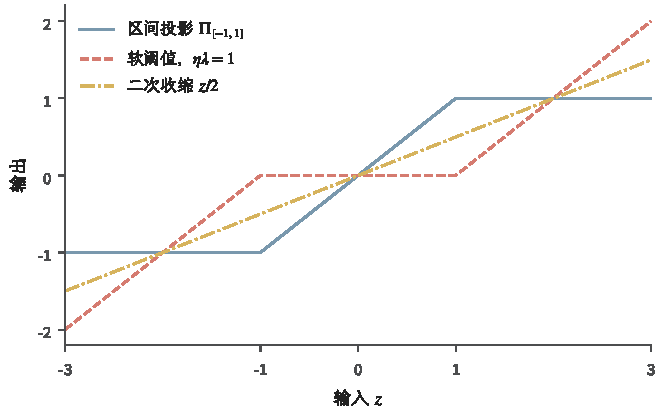
\includegraphics[width=\linewidth]{figures/math-preparation/concept-revision-analysis-functional/proximal-comparison.pdf}
 \caption{同一输入$z$的三种邻近映射。投影采用$C=[-1,1]$；软阈值与二次收缩均取$\eta\lambda=1$，分别输出$\operatorname{sign}(z)(|z|-1)_+$和$z/2$。横轴刻度标出阈值位置，曲线由完整分段解析式生成。}
 \label{fig:opt-proximal-comparison}
\end{figure}

邻近算子不会放大输入距离。令
$\bm{p}=\operatorname{prox}_{\eta r}(\bm{x})$、
$\bm{q}=\operatorname{prox}_{\eta r}(\bm{y})$。最优性条件给出
$(\bm{x}-\bm{p})/\eta\in\partial r(\bm{p})$和
$(\bm{y}-\bm{q})/\eta\in\partial r(\bm{q})$。把两个次梯度不等式相加，得到
\[
  \langle\bm{x}-\bm{y},\bm{p}-\bm{q}\rangle
  \geq\lVert\bm{p}-\bm{q}\rVert_2^2.
\]
再用Cauchy--Schwarz不等式便有
$\lVert\bm{p}-\bm{q}\rVert_2\leq\lVert\bm{x}-\bm{y}\rVert_2$。
这个非扩张性质依赖凸次梯度的单调性；非凸邻近子问题可能多解，不能直接沿用。

本节的凸次梯度也不同于第~\ref{chap:mathematical-analysis}章介绍的Clarke广义梯度。
前者用一个全局仿射下界定义，直接产生凸最优性条件；后者取局部Lipschitz函数邻近可微点
梯度极限的闭凸包，允许非凸局部结构。人为指定的替代梯度更只是反向计算信号，未必属于
前面任一集合。三者名称相近，定义对象与可用结论并不相同。

\begin{table*}[htbp]
 \centering\small
 \begin{tabularx}{\linewidth}{@{}lXX@{}}
 \toprule
 更新方式 & 每步处理的结构 & 分析前需核对的条件\\
 \midrule
 梯度下降 & 使用可微目标的梯度 & 光滑常数与步长；全局最优保证还依赖凸性或PL等条件\\
 投影梯度 & 梯度更新后求可行集最近点 & 非空闭凸集；投影本身的计算成本\\
 次梯度更新 & 使用非光滑凸目标的全局下界斜率 & 次梯度范数及步长序列；单步目标未必下降\\
 近端梯度 & 光滑部分求梯度，非光滑部分求邻近解 & 光滑部分的步长、正则项的适当闭凸性及可解邻近子问题\\
 \bottomrule
 \end{tabularx}
 \caption{常见一阶更新的结构与条件。相近的更新形式并不共享同一收敛定理。}
 \label{tab:opt-first-order-structures}
\end{table*}

\subsubsection{惩罚、约束与参数表达}

惩罚与硬约束有联系，但不是逐参数自动等价。考虑约束问题
\[
  \min_{\bm{w}}f(\bm{w})
  \quad\text{s.t.}\quad
  \lVert\bm{w}\rVert_1\leq R.
\]
若该问题有原始最优解，强对偶成立，并且对偶最优乘子
$\lambda^\star$确实达到，例如满足前述Slater条件且最优值有限，则原始最优解同时最小化
$f(\bm{w})+\lambda^\star\lVert\bm{w}\rVert_1$；Lagrangian中的常数
$-\lambda^\star R$不影响最小点。仅有原、对偶最优值相等并不能保证这样的有限乘子存在。
反过来，不同$\lambda$对应的范数半径可能相同，非凸问题还可能存在对偶间隙。把
$\bm{w}$写成其他参数的函数也会改变优化几何；即使表示同一预测函数，也不保证产生同一
更新轨迹。

同样的区别出现在权重衰减中。普通欧氏梯度下降用于
$f(\bm{w})+\lambda\lVert\bm{w}\rVert_2^2/2$时给出
\[
  \bm{w}^{(t+1)}
  =(1-\eta\lambda)\bm{w}^{(t)}-\eta\nabla f(\bm{w}^{(t)}),
\]
与直接乘上衰减因子相同。若使用预条件矩阵$\bm{P}$，惩罚梯度产生
$-\eta\lambda\bm{P}\bm{w}^{(t)}$，而坐标无关的直接衰减仍为
$-\eta\lambda\bm{w}^{(t)}$；除非$\bm{P}=\bm{I}$或另有匹配，它们不再相同。

\subsection{随机梯度与更新稳定性}
\label{sec:opt-stochastic-gradient-stability}

\subsubsection{随机梯度与带误差迭代}

有限和目标
\[
  F_S(\bm{w})=\frac1n\sum_{i=1}^n\ell_i(\bm{w})
  +\frac{\lambda}{2}\lVert\bm{w}\rVert_2^2
\]
的经验损失梯度要读取全部$n$项。这里的抽取先只用有限概率权重理解，$\mathbb E_I$表示按这些权重求和；
条件期望和随机收敛留待概率与随机过程章节。若$I$在$\{1,\ldots,n\}$上均匀抽取，则完整目标的
随机梯度可取
\[
  \bm{g}_I(\bm{w})
  =\nabla\ell_I(\bm{w})+\lambda\bm{w},\qquad
  \mathbb{E}_I[\bm{g}_I(\bm{w})]
  =\nabla F_S(\bm{w}).
\]
若按概率$p_i>0$非均匀抽取，则应改用
\[
  \bm{g}_I(\bm{w})
  =\frac{\nabla\ell_I(\bm{w})}{np_I}+\lambda\bm{w}.
\]
正则项梯度$\lambda\bm{w}$是确定量，无需抽样；小批量只需平均若干经过相应加权的
损失梯度，再加上这项确定梯度。小批量降低方差，却增加每步计算。

在概率工具建立前，可以先分析带确定误差的更新
\[
  \bm{w}^{(t+1)}
  =\bm{w}^{(t)}-\eta_t
  \bigl(\nabla F(\bm{w}^{(t)})+\bm{e}^{(t)}\bigr).
\]
若$F$为$L$光滑且$0<\eta_t\leq1/L$，把这一步代入下降引理，并对交叉项使用
Cauchy--Schwarz与$2ab\leq a^2+b^2$，可得
\[
  F(\bm{w}^{(t+1)})
  \leq F(\bm{w}^{(t)})
  -\frac{\eta_t}{2}\lVert\nabla F(\bm{w}^{(t)})\rVert_2^2
  +\frac{\eta_t}{2}\lVert\bm{e}^{(t)}\rVert_2^2.
\]
误差项因而必须与所求结论一起累计。固定非零偏差通常只允许迭代接近一个误差邻域；
$\sum_t\eta_t\lVert\bm{e}^{(t)}\rVert_2^2<\infty$使上述目标下降不等式中的累计
误差项有限。仅令
$\eta_t\to0$仍不够，还要核对步长总量是否足以持续纠偏，以及目标与迭代是否保持稳定。

若理想更新映射$T_t(\bm{w})=\bm{w}-\eta_t\nabla F(\bm{w})$是
$\rho_t$-Lipschitz，实际轨迹与理想轨迹之差$\delta_t$满足
\begin{equation}
  \delta_{t+1}\leq\rho_t\delta_t+\eta_t\lVert\bm{e}^{(t)}\rVert_2.
  \label{eq:opt-inexact-gradient-recurrence}
\end{equation}
展开递推可见，$\rho_t<1$时旧误差会衰减；若只有$\rho_t\leq1$，直接求和控制轨迹偏差
需要考察$\sum_t\eta_t\lVert\bm{e}^{(t)}\rVert_2$，前面的平方误差条件一般不能推出
这个一次范数条件。若$\rho_t>1$，传播因子还可能放大早期扰动。减小步长降低单步误差
影响，也会减慢理想更新。

\subsubsection{成对迭代与梯度自界}

同一递推可比较只替换一个样本的数据集$S,S'$。若每个样本梯度有界，且两条轨迹在使用
相同样本时由收缩映射拉近，只在抽到被替换样本时受到额外扰动，就能控制
$\lVert\bm{w}_S^{(t)}-\bm{w}_{S'}^{(t)}\rVert_2$。具体地，设每个样本梯度
$L$-Lipschitz且范数不超过$G$，两条迭代使用相同索引$I_t$。记距离为$\Delta_t$；
若$I_t$不是被替换的索引，则
\[
  \Delta_{t+1}\leq(1+\eta_tL)\Delta_t;
\]
若恰好抽到被替换项，则再增加至多$2\eta_tG$。在凸光滑且步长适当时，共同样本的梯度
更新可进一步证明为非扩张映射，从而去掉前式中的膨胀因子。这称为
\term{算法稳定性}（algorithmic stability）：训练集改动一个样本时，输出不会变化太大。
完整的期望界和随机收敛需使用第~\ref{chap:stochastic-processes-and-approximation}章的
条件期望与噪声工具。

缩放损失会等比例缩放梯度，因此学习率不能脱离损失尺度比较。梯度裁剪把过大更新限制在
指定半径内，改变了估计量并可能引入偏差。对更新式直接减去
$\eta\lambda\bm{w}$的权重衰减，在普通梯度下降中等价于$\ell_2$惩罚；使用坐标自适应缩放
时，两者通常不再等价。

\begin{lemma}[非负光滑函数的梯度自界]
\label{lem:opt-self-bounding}
若$\ell:\mathbb{R}^d\to[0,\infty)$可微且$L$光滑，其中$L>0$，则
\[
  \lVert\nabla\ell(\bm{w})\rVert_2^2\leq2L\ell(\bm{w}).
\]
\end{lemma}

\begin{proof}
在下降引理中取
$\bm{v}=\bm{w}-\nabla\ell(\bm{w})/L$，得到
\[
  \ell(\bm{v})
  \leq\ell(\bm{w})-\frac{1}{2L}
  \lVert\nabla\ell(\bm{w})\rVert_2^2.
\]
左侧非负，移项即得结论。若损失可取负值，这一步失效；给函数加常数虽不改变梯度，却会
改变右侧，所以非负性是实质条件。
\end{proof}

\section{变量分解与多层决策}
\label{sec:opt-decomposition-multiple-levels}

前面主要比较同一目标下的更新规则。现在考察问题自身的组织：参数可分块，
目标可能彼此竞争，某些变量还可能由另一个优化问题决定。分块方法利用变量结构，
多目标与鞍点明确不同目标之间的关系，双层求导则追踪内层解如何影响外层目标。
这些结构可以与光滑、约束或随机条件组合，不能按单一的算法优劣排序。

\subsection{分块、交替与分布优化}
\label{sec:opt-block-alternating-distribution}

\subsubsection{分块更新与约束分解}

若变量自然分成$\bm{u}$与$\bm{v}$两组，可以固定一组更新另一组。对
\[
  \Phi(\bm{u},\bm{v})
  =\frac12\lVert\bm{X}\bm{u}+\bm{Z}\bm{v}-\bm{y}\rVert_2^2
  +r(\bm{u})+s(\bm{v}),
\]
\term{分块坐标法}（block coordinate method）每次只对一个块走梯度或近端步；
\term{交替最小化}（alternating minimization）则精确或近似求解每个块的条件子问题。
若每次子问题确实降低同一个
$\Phi$，目标值单调不增。精确交替最小化时，这一点直接来自
\[
  \Phi(\bm{u}^{(t+1)},\bm{v}^{(t)})
  \leq\Phi(\bm{u}^{(t)},\bm{v}^{(t)}),\qquad
  \Phi(\bm{u}^{(t+1)},\bm{v}^{(t+1)})
  \leq\Phi(\bm{u}^{(t+1)},\bm{v}^{(t)}).
\]
但非凸情形下仍可能停在局部解或依赖初始化。

一个可复核的耦合二次例子是
\[
  \Phi(u,v)=\frac12(u-v)^2+\frac12(u-1)^2.
\]
固定$v$时的唯一最优点为$u=(v+1)/2$，固定$u$时的唯一最优点为$v=u$。从
$v^{(0)}$出发，一轮交替更新得到
$u^{(t+1)}=(v^{(t)}+1)/2$、$v^{(t+1)}=u^{(t+1)}$，因而
$v^{(t+1)}-1=(v^{(t)}-1)/2$，最终到达联合最优点$(1,1)$。这里的收敛来自这个
正定二次目标的特殊结构。换成非凸目标$(uv-1)^2$并从$(0,0)$开始时，逐块目标在一块
固定为零时没有提供离开零点的理由；若平局规则继续选择零，目标保持为$1$，而全局最优值
为$0$。所以逐块精确和目标单调都不单独保证全局最优。

约束耦合时，可以复制共享变量，再通过一致性约束分解为局部子问题。乘子负责协调副本，
这改变了每步计算位置，却没有删除原约束。若局部问题没有被足够准确地求解，或协调步长
不满足条件，分解形式本身不保证收敛。

\subsubsection{分布变量与可行约束}

变量也可以是一个分布$q$。此时“更新分布”仍是在某个可行分布集合上降低同一目标，而非
一种脱离优化的概率操作。在有限支持$\{1,\ldots,m\}$上，分布变量就是概率单纯形
\[
  \bm{\Delta}_m
  =\{\bm{q}\in\mathbb{R}^m:q_i\geq0,\ \sum_{i=1}^m q_i=1\}.
\]
归一化、非负性和支持集都是可行约束，更新后必须仍留在这个单纯形中。EM与变分方法还需要
期望、条件分布和散度。第~\ref{chap:probability-theory}章、
第~\ref{chap:mathematical-statistics}章和
第~\ref{chap:information-theory-and-statistical-geometry}章建立这些对象后，将复用
交替优化与MM的单调性核对方式。

\subsection{多目标与鞍点}
\label{sec:opt-multiobjective-saddle}

\subsubsection{支配、Pareto与共同下降}

一个标量不能完整表示互相竞争的任务，需先规定怎样比较损失向量。
\begin{definition}[支配与Pareto最优]
\label{def:opt-pareto-optimality}
设$C$为非空可行集合，$\bm f=(f_1,\ldots,f_m):C\to\mathbb R^m$，各分量均要最小化。
若$\bm u,\bm v\in C$满足所有$i$都有$f_i(\bm u)\leq f_i(\bm v)$，且至少一项严格小于，
就称$\bm u$\term{支配}（dominate）$\bm v$。不可被任何可行方案支配的点称为
\term{Pareto最优}（Pareto optimal）。
\end{definition}
分量逐项不大于给出偏序；这里的严格支配是相应的严格比较，不是单一排名。
下文先用两个目标说明这种区别。

加权和$\alpha f_1+(1-\alpha)f_2$把偏好写成一个标量目标，$\alpha\in[0,1]$。
它能找出凸目标像边界上的支撑点，但非凸Pareto前沿的某些点无法由任何固定权重得到。
例如三个可行方案的损失向量分别为$(0,1)$、$(1,0)$和$(0.6,0.6)$。第三个方案不被
前两个方案支配，所以是Pareto最优；但对任意$\alpha\in[0,1]$，前两个方案的加权损失
中至少一个不超过$0.5$，严格小于第三个方案的$0.6$，故权重和永远不会选择第三个方案。
在当前点，方向$\bm{d}$若满足
\[
  \langle\nabla f_1(\bm{w}),\bm{d}\rangle<0,\qquad
  \langle\nabla f_2(\bm{w}),\bm{d}\rangle<0,
\]
就是\term{共同下降方向}（common descent direction）。寻找最小范数凸组合
$\alpha\nabla f_1+(1-\alpha)\nabla f_2$相当于把原点投影到两梯度的线段上。

\begin{theorem}[无共同下降方向的一阶判定]
\label{thm:opt-common-descent}
对可微的$m$个目标，在无约束点$\bm{w}$处不存在共同严格下降方向，当且仅当存在
$\alpha_i\geq0$、$\sum_i\alpha_i=1$，使
$\sum_i\alpha_i\nabla f_i(\bm{w})=\bm{0}$。
\end{theorem}

\begin{proof}
若这样的凸组合存在，而$\bm{d}$使每个内积都为负，则加权和内积也为负，与零向量矛盾。
反之，若原点不在梯度集合的凸包中，定理~\ref{thm:opt-projection-separation}给出
$\bm{d}$，使它与每个梯度的内积具有同一严格符号；必要时取$-\bm{d}$，便得到共同严格
下降方向。
\end{proof}

这个条件只排除局部的一阶共同改善，不保证全局Pareto最优；高阶变化或远处方案仍可能
同时改善所有目标。

\subsubsection{极小极大与鞍点间隙}

另一类问题让两个变量方向相反：
\[
  \min_{\bm{w}\in W}\max_{\bm{z}\in Z}\phi(\bm{w},\bm{z}).
\]
\begin{definition}[极小极大鞍点]
\label{def:opt-minimax-saddle}
设$W,Z$非空，$\phi:W\times Z\to\mathbb R$。点$(\bm w^\star,\bm z^\star)\in W\times Z$若对所有
$\bm w\in W,\bm z\in Z$满足
\[
  \phi(\bm{w}^{\star},\bm{z})
  \leq\phi(\bm{w}^{\star},\bm{z}^{\star})
  \leq\phi(\bm{w},\bm{z}^{\star})
\]
就称为\term{极小极大鞍点}（minimax saddle point）。
\end{definition}
这里“鞍点”描述两个变量承担
相反优化方向时的全局比较关系，不是第~\ref{sec:analysis-second-order-curvature}节中
由单个标量函数的驻点和Hessian矩阵正负曲率定义的微分鞍点。微分鞍点未必求解某个极小
极大问题；极小极大鞍点位于边界或目标不可微时，也未必满足驻点与Hessian判据。
对任意候选对定义
\[
  P(\bm{w})=\sup_{\bm{z}\in Z}\phi(\bm{w},\bm{z}),\qquad
  D(\bm{z})=\inf_{\bm{w}\in W}\phi(\bm{w},\bm{z}).
\]
总有$D(\bm{z})\leq P(\bm{w})$，所以
$P(\bm{w})-D(\bm{z})\geq0$是\term{原始--对偶间隙}
（primal--dual gap）；间隙为零时，该候选对满足鞍点不等式。

本章采用以下有限维极小极大版本：若$W,Z$非空、紧且凸，$\phi$连续，对固定
$\bm{z}$的$\phi(\cdot,\bm{z})$为凸函数，对固定$\bm{w}$的
$\phi(\bm{w},\cdot)$为凹函数，则
\[
  \min_{\bm{w}\in W}\max_{\bm{z}\in Z}\phi(\bm{w},\bm{z})
  =
  \max_{\bm{z}\in Z}\min_{\bm{w}\in W}\phi(\bm{w},\bm{z}),
\]
且两侧最值达到。紧致性提供最值的达到，凸凹性允许用分离比较混合候选，连续性保证极限
不丢失函数值。鲁棒优化中的$\bm{z}$表示最坏扰动，对抗训练让扰动方提高损失，多任务协调
则可能在权重与模型间形成极小极大结构。若缺少上述条件，两个优化次序可能不同；即使值相等，
具体梯度下降--上升仍可能旋转或发散，值的存在定理不等于算法收敛定理。

\subsection{双层目标与隐式更新}
\label{sec:opt-bilevel}

\subsubsection{有限步更新的展开求导}

有些决策必须先经过一次学习过程才能评价。令外层变量为$\bm{\theta}$。如果内层问题有
多个最小点，只写
$\bm{w}^{\star}(\bm{\theta})\in
\argmin_{\bm{w}}L_{\mathrm{in}}(\bm{w},\bm{\theta})$
并不能定义一个单值映射，不同最小点还可能给出不同的外层损失。此时可以分别把最小点集合
上的最小、最大外层损失定义为乐观、悲观值，也可以给定由初始化和算法路径决定的单值
选择规则。下文假设内层最小解唯一，或已经给定单值选择$S$，并记
\[
  \bm{w}^{\star}(\bm{\theta})=S(\bm{\theta})
  \in\argmin_{\bm{w}}L_{\mathrm{in}}(\bm{w},\bm{\theta}).
\]
于是外层目标
\begin{equation}
  J(\bm{\theta})
  =L_{\mathrm{out}}(\bm{w}^{\star}(\bm{\theta}),\bm{\theta}).
  \label{eq:opt-bilevel-objective}
\end{equation}
这就是\term{双层优化}（bilevel optimization）。元学习把内层看成任务适应，超参数
选择让$\bm{\theta}$控制正则强度或数据权重，定向知识修正则让外层评价修改后的特定行为。

一种求导方式是把$T$步内层更新全部展开。例如
$\bm{w}^{(t+1)}=\bm{w}^{(t)}-\eta\nabla_{\bm{w}}
L_{\mathrm{in}}(\bm{w}^{(t)},\bm{\theta})$，再按链式法则从$t=T$反向传播。
展开法忠实求导于“运行$T$步”这个实际算法，但存储随$T$增长，且所得梯度对应近似内层解，
不一定对应精确最优解。

两步展开已经能看清链式结构。记
\[
  \bm{A}_t=\bm{I}-\eta\nabla_{\bm{w}\bm{w}}^2
  L_{\mathrm{in}}(\bm{w}^{(t)},\bm{\theta}),\qquad
  \bm{B}_t=\nabla_{\bm{w}\bm{\theta}}^2
  L_{\mathrm{in}}(\bm{w}^{(t)},\bm{\theta}).
\]
则
\[
  \frac{d\bm{w}^{(t+1)}}{d\bm{\theta}}
  =\bm{A}_t\frac{d\bm{w}^{(t)}}{d\bm{\theta}}-\eta\bm{B}_t,
\]
从而
\[
  \frac{d\bm{w}^{(2)}}{d\bm{\theta}}
  =\bm{A}_1\bm{A}_0\frac{d\bm{w}^{(0)}}{d\bm{\theta}}
  -\eta\bm{A}_1\bm{B}_0-\eta\bm{B}_1.
\]
外层梯度再把这个Jacobian与
$\nabla_{\bm{w}}L_{\mathrm{out}}$相乘，并加上外层目标对$\bm{\theta}$的直接偏导。
截断某一步会删除相应乘积项，因而改变所求导的算法，而不只是节省存储。

\subsubsection{局部内层解的隐式求导}

隐式求导跟踪的是一个选定的非退化局部最小点分支，不自动证明该分支实现全局最小值。
只有当这个分支也是全局最小点并符合前述选择规则时，它才与
$\bm{w}^{\star}(\bm{\theta})$及$J$对应。为区分两者，记局部分支及其外层目标为
$\widehat{\bm{w}}(\bm{\theta})$和
$\widehat{J}(\bm{\theta})
=L_{\mathrm{out}}(\widehat{\bm{w}}(\bm{\theta}),\bm{\theta})$。
若$L_{\mathrm{in}}$二阶连续可微，并且
\[
  \nabla_{\bm{w}}L_{\mathrm{in}}
  (\widehat{\bm{w}}(\bm{\theta}),\bm{\theta})=\bm{0},
\]
记在该分支上计算的二阶导数为
$\bm{H}_{ww}=\nabla_{\bm{w}\bm{w}}^2L_{\mathrm{in}}$和
$\bm{H}_{w\theta}=\nabla_{\bm{w}\bm{\theta}}^2L_{\mathrm{in}}$。
对驻点方程关于$\bm{\theta}$求导得到
\[
  \bm{H}_{ww}\frac{d\widehat{\bm{w}}}{d\bm{\theta}}
  +\bm{H}_{w\theta}=\bm{0}.
\]
当$\bm{H}_{ww}$可逆时，隐函数定理给出局部可微分支；对非退化局部最小点，
$\bm{H}_{ww}\succ\bm{0}$保证这一可逆性。链式法则于是给出
\begin{equation}
  \nabla_{\bm{\theta}}\widehat{J}
  =
  \nabla_{\bm{\theta}}L_{\mathrm{out}}
  -\bm{H}_{w\theta}^{\top}
  \bm{H}_{ww}^{-\top}
  \nabla_{\bm{w}}L_{\mathrm{out}}.
  \label{eq:opt-implicit-hypergradient}
\end{equation}
式~\eqref{eq:opt-implicit-hypergradient}是\term{隐式超梯度}
（implicit hypergradient）。实际计算通常解线性方程
$\bm{H}_{ww}^{\top}\bm{v}=\nabla_{\bm{w}}L_{\mathrm{out}}$，无须显式求逆。

用二次内层目标可以核对公式。设$\bm{H}\succ\bm{0}$，
\[
  L_{\mathrm{in}}(\bm{w},\bm{\theta})
  =\frac12(\bm{w}-\bm{B}\bm{\theta})^{\top}
  \bm{H}(\bm{w}-\bm{B}\bm{\theta}),\qquad
  L_{\mathrm{out}}(\bm{w})
  =\frac12\lVert\bm{C}\bm{w}-\bm{d}\rVert_2^2.
\]
这里内层最小点唯一，因此局部分支与全局选择一致：
$\widehat{\bm{w}}=\bm{w}^{\star}=\bm{B}\bm{\theta}$且
$\widehat{J}=J$。直接消元给出
\[
  \nabla_{\bm{\theta}}J
  =\bm{B}^{\top}\bm{C}^{\top}
  (\bm{C}\bm{B}\bm{\theta}-\bm{d}).
\]
隐式公式中$\bm{H}_{ww}=\bm{H}$、
$\bm{H}_{w\theta}=-\bm{H}\bm{B}$，代入后得到同一结果。计算时若线性方程残差为
$\bm{r}$，解误差为$\bm{H}^{-\top}\bm{r}$；小特征值会放大该误差。因而内层驻点残差、
线性求解残差和曲率病态是三种不同的误差来源。

若内层只近似收敛，驻点残差会进入超梯度误差；若Hessian矩阵奇异，解映射可能不唯一或不可微；
若内层非凸，所选局部分支还依赖初始化与算法路径，并且可能不是全局最小点。后一种情况下，
式~\eqref{eq:opt-implicit-hypergradient}给出的是$\widehat{J}$的梯度，而不是前述全局
双层目标$J$的梯度。展开深度、线性方程精度、内层计算预算与解选择规则因此都是问题定义的
一部分，而不只是实现细节。

\section{本章小结}
\label{sec:opt-summary}

最优化需要分别回答四个问题：候选解是否存在，某个点为何最优，算法怎样到达它，以及误差
按什么尺度收敛。连续性配合紧致性保证存在；在闭域上，下半连续性与强制性也能通过紧
下水平集保证存在。凸性把局部条件提升为全局条件，强凸、光滑性与PL条件则分别控制参数
距离、单步上界和目标误差。它们不能只用“曲率好”一语合并。

带资源约束后，KKT条件描述目标梯度与约束法向量的平衡，对偶变量提供界和敏感性解释。
Farkas证书与线性规划强对偶说明最优值相等需要证明，不能从凸性直接跳得。松弛、对偶界与
可行解共同形成最优性证书；证书说明结果离最优值多远，却不自动给出寻找结果的过程。

非光滑正则需要次梯度、投影或邻近算子，不完整梯度需要核对误差如何累计。分块、分布变量、
多目标、鞍点与双层目标改变的是变量组织和最优性概念，不能沿用同一套无条件保证。随机更新
的严格收敛将在第~\ref{chap:stochastic-processes-and-approximation}章建立条件期望与
噪声工具后补全；后续决策章节还会复用本章的对偶与鞍点语言。紧邻的
第~\ref{chap:functional-analysis-and-approximation}章将把有限维参数推广到函数空间，
区分表示存在性、逼近误差与函数类复杂度。

\chapter{泛函分析与逼近理论}
\label{chap:functional-analysis-and-approximation}

有限维模型常把函数写成固定基函数的线性组合：
\begin{equation}
  f_m(x)=\sum_{j=1}^{m}a_j\phi_j(x).
  \label{eq:functional-finite-basis-expansion}
\end{equation}
当$m$固定时，可以把系数$(a_1,\ldots,a_m)^{\top}$当作普通向量，用欧氏距离比较两个
候选解。然而，一旦允许基函数数目增加，系数向量所在的维数也随之改变；同一个函数还可能
在不同基下拥有完全不同的系数。此时，仅比较参数向量已经不能稳定地回答三个问题：函数
之间相差多少，有限表示能否逼近目标，以及从数据选择出的函数有多复杂。

本章改为直接把函数看成空间中的点。范数规定误差怎样度量，完备性保证逼近序列的极限仍在
空间内，内积则把有限维最小二乘中的正交与投影推广到函数。若还要求能够连续地读取函数在
某个输入处的值，就会得到再生核Hilbert空间（reproducing kernel Hilbert space, RKHS）。
核谱在选定测度后解释全域方向与正则化尺度。在此基础上，再区分表示能力与函数类大小：前者问某个目标能否被逼近，后者问候选函数
可以沿多少方向、以多细尺度变化。这一区分将在后续概率章节中进入有限观测误差，但本章只
建立其中不依赖随机抽样的空间结构。

\section{函数作为空间中的对象}
\label{sec:functional-functions-as-space-elements}

\subsection{函数空间的线性结构}

设$\mathcal{X}$为输入集合，$\mathbb{R}^{\mathcal{X}}$表示从$\mathcal{X}$到
$\mathbb{R}$的全部函数。对$f,g\in\mathbb{R}^{\mathcal{X}}$和$a,b\in\mathbb{R}$，
定义
\[
  (af+bg)(x)=af(x)+bg(x),\qquad x\in\mathcal{X}.
\]
这些逐点运算使$\mathbb{R}^{\mathcal{X}}$成为向量空间。式
\eqref{eq:functional-finite-basis-expansion}描述的集合只是其中由
$\phi_1,\ldots,\phi_m$张成的有限维子空间。允许无限多个基方向以后，线性结构仍然
存在，但坐标数目不再适合作为唯一的大小尺度。

函数可以相加，并不表示已经知道两个函数相差多少。把误差汇总成一个非负数，还要要求
缩放与累加时的误差具有一致规则；这正是范数的作用。
\begin{definition}[赋范空间]
\label{def:functional-normed-space}
设$\mathcal V$为实向量空间。映射$\lVert\cdot\rVert_{\mathcal V}:\mathcal V\to[0,\infty)$
若对任意$f,g\in\mathcal V$和$a\in\mathbb R$满足
\[
  \lVert f\rVert_{\mathcal{V}}\geq0,\qquad
  \lVert f\rVert_{\mathcal{V}}=0\Longleftrightarrow f=0,\qquad
  \lVert af\rVert_{\mathcal{V}}=|a|\lVert f\rVert_{\mathcal{V}},
\]
以及三角不等式
$\lVert f+g\rVert_{\mathcal{V}}\leq
\lVert f\rVert_{\mathcal{V}}+\lVert g\rVert_{\mathcal{V}}$。
则称为范数，$(\mathcal V,\lVert\cdot\rVert_{\mathcal V})$称为\term{赋范空间}
（normed space）。它诱导距离$d(f,g)=\lVert f-g\rVert_{\mathcal V}$。
\end{definition}
选择不同范数，就是选择不同的误差含义。范数必须为每个空间元素给出有限值；因此，
选定积分范数后，还要把不满足相应可积条件的函数排除在空间之外。

例如，紧区间$[a,b]$上的连续函数空间$C([a,b])$常使用一致范数
\[
  \lVert f\rVert_{\infty}
  =\sup_{x\in[a,b]}|f(x)|.
\]
这个范数控制每个输入上的最大误差。若$\mu$是一个测度，则第
\ref{chap:mathematical-analysis}章建立的$L^p(\mu)$空间使用
\[
  \lVert f\rVert_{L^p(\mu)}
  =
  \left(\int_{\mathcal{X}}|f(x)|^p\,\mathrm{d}\mu(x)\right)^{1/p},
  \qquad 1\leq p<\infty.
\]
它控制的是相对于$\mu$的整体误差，允许函数在小测度集合上偏离较大。两种误差不能互相
替代：在$[0,1]$上令
\[
  f_n(x)=\max\{1-nx,0\},
\]
则$\lVert f_n\rVert_{L^2}^2=1/(3n)\to0$，但
$\lVert f_n\rVert_{\infty}=1$始终不变。

\begin{figure}[htbp]
 \centering
 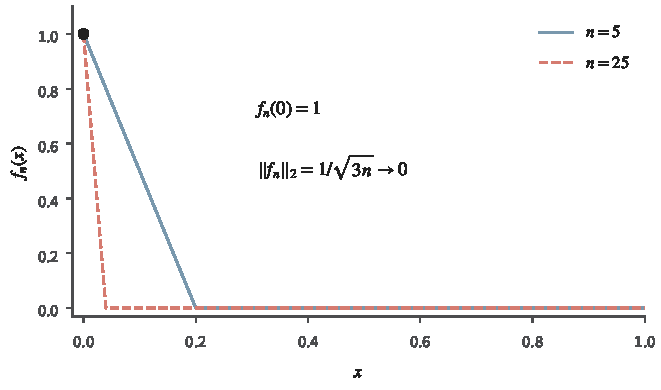
\includegraphics[width=\linewidth]{figures/math-preparation/analysis-geometry/functional-point-evaluation.pdf}
 \caption{连续尖峰$f_n(x)=\max\{1-nx,0\}$在$L^2$范数下趋于零，原点函数值却始终为$1$。峰宽分别为$1/5$和$1/25$；蓝、红线均由解析式生成。整体能量控制不等于稳定的点值控制。}
 \label{fig:functional-point-evaluation}
\end{figure}

后面的完备性证明会用到$L^2$版本的\term{Minkowski不等式}
（Minkowski inequality），也就是$L^2$范数的三角不等式。对$f,g\in L^2(\mu)$，
Cauchy--Schwarz不等式给出
\[
  \begin{aligned}
  \lVert f+g\rVert_{L^2(\mu)}^2
  &=
  \lVert f\rVert_{L^2(\mu)}^2
  +
  2\int_{\mathcal{X}}f(x)g(x)\,\mathrm{d}\mu(x)
  +\lVert g\rVert_{L^2(\mu)}^2\\
  &\leq
  \bigl(
    \lVert f\rVert_{L^2(\mu)}
    +
    \lVert g\rVert_{L^2(\mu)}
  \bigr)^2.
  \end{aligned}
\]
两边开平方便得到
$\lVert f+g\rVert_{L^2(\mu)}
\leq\lVert f\rVert_{L^2(\mu)}+\lVert g\rVert_{L^2(\mu)}$；
反复使用即可控制有限个函数之和。

\subsection{Banach空间与完备性}

不断增加基函数时，可能得到越来越接近的候选函数，却始终没有一个有限表示等于极限。
分析章的完备性在这里要求：这些候选若按所选范数形成柯西序列，空间就应容纳它们的极限。
\begin{definition}[Banach空间]
\label{def:functional-banach-space}
若赋范空间$\mathcal V$在诱导距离$d(f,g)=\lVert f-g\rVert_{\mathcal V}$下完备，
即每个范数柯西序列都在该范数下收敛到$\mathcal V$中的元素，则称其为
\term{Banach空间}（Banach space）。
\end{definition}
完备性不负责证明某个具体
序列是柯西序列；它只保证一旦误差足以让序列内部彼此靠近，极限不会落到空间之外。

区间$[a,b]$上的$C([a,b])$配备一致范数是Banach空间。事实上，若$(f_n)$在一致范数
下为柯西序列，那么每个$x$处的$(f_n(x))$都是实数柯西序列，可以定义
$f(x)=\lim_n f_n(x)$。柯西条件对所有$x$使用同一个$N$，故$f_n$一致收敛到$f$；
连续函数的一致极限仍连续，所以$f\in C([a,b])$。

同一个函数集合换一种范数可能失去完备性。连续函数空间$C([0,1])$配备$L^2$范数就
不是完备的。取连续函数$f_n$逐渐逼近阶跃函数
$\mathbb{I}\{x>1/2\}$，可以使$(f_n)$在$L^2$中为柯西序列，但它的$L^2$极限没有
任何处处连续的代表元。完成这个空间需要加入可测函数的几乎处处等价类，得到
$L^2([0,1])$。这里“几乎处处等价”很关键：如果$f$与$g$只在零测集上不同，它们在
$L^2$中是同一个元素。

$L^2(\mu)$本身的完备性可以从柯西列内部构造极限。设$(f_n)$在$L^2(\mu)$中为
柯西列。逐次选取子列$(f_{n_k})$，使
\[
  \lVert f_{n_{k+1}}-f_{n_k}\rVert_{L^2(\mu)}
  \leq 2^{-k}.
\]
令$h_k=|f_{n_{k+1}}-f_{n_k}|$。对有限部分和反复使用上面的$L^2$版Minkowski
不等式，再用Fatou引理，可得
\[
  \int_{\mathcal{X}}
  \left(\sum_{k=1}^{\infty}h_k\right)^2
  \,\mathrm{d}\mu
  \leq
  \left(\sum_{k=1}^{\infty}2^{-k}\right)^2
  <\infty.
\]
因此$\sum_k h_k(x)$几乎处处有限，$(f_{n_k}(x))$在这些点绝对收敛。把它的几乎处处
极限记为$f$。同样对尾和使用Fatou引理，得到
\[
  \lVert f_{n_\ell}-f\rVert_{L^2(\mu)}
  \leq
  \sum_{k=\ell}^{\infty}2^{-k}
  \longrightarrow0.
\]
原序列是柯西列，故它与已收敛子列的距离也趋于零，从而$f_n\to f$于$L^2(\mu)$。
这个论证同时说明为何要把只在零测集上不同的代表元视为同一元素：构造得到的点态极限
本来就只在几乎处处意义下确定。对$1\leq p<\infty$可用相同的可求和子列思路证明
$L^p(\mu)$完备；$p=\infty$时则控制本质上确界。因此，$1\leq p\leq\infty$时的
$L^p(\mu)$都是Banach空间，而$L^2(\mu)$还具有下面要用的内积结构。

\subsection{Hilbert空间与内积}

范数给出长度和距离，却未必能定义夹角。要把最小二乘的正交残差推广到函数，需要再加入
能够比较两个方向的内积。
\begin{definition}[实内积空间与Hilbert空间]
\label{def:functional-hilbert-space}
\term{内积空间}（inner-product space）在实向量空间$\mathcal{V}$上配备对称双线性
映射$\langle\cdot,\cdot\rangle_{\mathcal{V}}:\mathcal V\times\mathcal V\to\mathbb R$，并要求
$\langle f,f\rangle_{\mathcal{V}}>0$对每个非零$f$成立。内积诱导范数
\[
  \lVert f\rVert_{\mathcal{V}}
  =\sqrt{\langle f,f\rangle_{\mathcal{V}}}.
\]
相应范数下完备的内积空间称为\term{Hilbert空间}（Hilbert space）。
\end{definition}
它把欧氏空间中
长度、夹角、正交和投影的关系保留下来，同时允许空间无限维。

$L^2(\mu)$是基本例子，其内积为
\[
  \langle f,g\rangle_{L^2(\mu)}
  =\int_{\mathcal{X}}f(x)g(x)\,\mathrm{d}\mu(x).
\]
但$L^1(\mu)$与一般的$L^p(\mu)$并不都由内积诱导。一个范数来自内积，当且仅当它满足
\term{平行四边形恒等式}（parallelogram identity）
\begin{equation}
  \lVert f+g\rVert^2+\lVert f-g\rVert^2
  =
  2\lVert f\rVert^2+2\lVert g\rVert^2.
  \label{eq:functional-parallelogram-identity}
\end{equation}
例如在$\mathbb{R}^2$的$L^1$范数中取
$\bm{u}=(1,0)^{\top}$、$\bm{v}=(0,1)^{\top}$，左侧为$8$，右侧为$4$，所以这个
范数不可能来自内积。Banach空间提供极限与距离，Hilbert空间额外提供正交几何；后面的
投影结论依赖后者，不能只靠完备范数得到。

无限维还使一些有限维中自动成立的性质需要单独检查。有限维子空间总是闭集，有界序列总能
抽出收敛子列，线性映射也自动连续；这些陈述在一般无限维空间中都可能失效。例如
$\ell^2$中的标准单位向量$(\bm{e}_j)_{j\geq1}$都位于单位球内，但$j\neq k$时
\[
  \lVert\bm{e}_j-\bm{e}_k\rVert_2=\sqrt{2}.
\]
这个序列没有柯西子列，因而也没有收敛子列。无限维闭单位球由此给出“闭且有界未必紧”
的具体反例；这里具体指$\ell^2$的闭单位球。

有限表示可能并未包含极限，却能任意接近它；这项逼近性质应与空间的完备性分开。
\begin{definition}[稠密子集]
\label{def:functional-density}
设$(\mathcal V,\lVert\cdot\rVert)$为赋范空间，$\mathcal F\subseteq\mathcal V$。
若对每个$f\in\mathcal V$和每个$\varepsilon>0$，存在$g\in\mathcal F$满足
$\lVert f-g\rVert<\varepsilon$，则称$\mathcal F$在$\mathcal V$中稠密。
等价地，$\mathcal F$在该范数诱导距离下的闭包等于$\mathcal V$。
\end{definition}
这里的闭包由原集合及所有能被它任意接近的点组成；稠密不要求这些点已属于$\mathcal F$。
完备性与稠密性也不能混为一谈。
$\ell^2$由平方可和序列$\bm{a}=(a_1,a_2,\ldots)$组成，范数为
$\lVert\bm{a}\rVert_2^2=\sum_{j=1}^{\infty}a_j^2$。只有有限个非零坐标的序列构成
子空间$c_{00}$，它在$\ell^2$中稠密却不闭。序列
$(1,1/2,\ldots,1/n,0,\ldots)$属于$c_{00}$，其极限
$(1,1/2,1/3,\ldots)$属于$\ell^2$但不属于$c_{00}$。这正是闭性在最佳逼近问题中
不能省略的原因。有限截断能够不断逼近$\ell^2$中的元素，说明$c_{00}$的闭包是
$\ell^2$；它并不说明$c_{00}$自身已经包含这些极限。

\section{正交展开与函数投影}
\label{sec:functional-orthogonal-expansions-projections}

范数空间允许比较函数并取极限，内积空间还可以辨认正交方向。
本节把有限维最小二乘中的最近点问题推广到函数空间：闭性、凸性和完备性分别保证可行极限、
唯一最近点和极限存在。正交展开由此获得误差分解，其有效性还取决于所选方向是否张成目标。

\subsection{闭凸集上的最近点}

有限维最小二乘把观测向量投影到设计矩阵的列空间。函数逼近的对应问题是：给定Hilbert
空间$\mathcal{H}$中的目标$f$与候选集合$C$，能否找到$g^\star\in C$使
$\lVert f-g^\star\rVert_{\mathcal{H}}$最小？下面的投影定理中，非空性只保证距离
下确界有候选可比较；凸性与内积几何先使最小化序列成为柯西列，Hilbert空间的完备性
保证该序列在空间中有极限，闭性再把极限留在$C$内。凸性还参与唯一性与变分不等式的
证明，因而不能把四项条件各自简化成互不相干的一项职责。

\begin{theorem}[Hilbert空间投影定理]
\label{thm:functional-hilbert-projection}
设$\mathcal{H}$为实Hilbert空间，$C\subseteq\mathcal{H}$非空、闭且凸。对每个
$f\in\mathcal{H}$，存在唯一的$g^\star\in C$满足
\[
  \lVert f-g^\star\rVert_{\mathcal{H}}
  =\inf_{g\in C}\lVert f-g\rVert_{\mathcal{H}}.
\]
这个最近点由变分不等式
\begin{equation}
  \langle f-g^\star,g-g^\star\rangle_{\mathcal{H}}
  \leq0,\qquad g\in C
  \label{eq:functional-convex-projection-characterization}
\end{equation}
唯一刻画。若$C=M$是闭线性子空间，则该条件等价于
\begin{equation}
  f-g^\star\perp M.
  \label{eq:functional-subspace-projection-orthogonality}
\end{equation}
\end{theorem}

\begin{proof}
记$d=\inf_{g\in C}\lVert f-g\rVert_{\mathcal{H}}$，并取最小化序列
$(g_n)\subseteq C$，使$\lVert f-g_n\rVert_{\mathcal{H}}\to d$。凸性保证
$(g_n+g_m)/2\in C$。把平行四边形恒等式用于
$f-g_n$与$f-g_m$，得到
\begin{align*}
  \lVert g_n-g_m\rVert_{\mathcal{H}}^2
  &=
  2\lVert f-g_n\rVert_{\mathcal{H}}^2
  +2\lVert f-g_m\rVert_{\mathcal{H}}^2\\
  &\quad
  -4\left\lVert
    f-\frac{g_n+g_m}{2}
  \right\rVert_{\mathcal{H}}^2\\
  &\leq
  2\lVert f-g_n\rVert_{\mathcal{H}}^2
  +2\lVert f-g_m\rVert_{\mathcal{H}}^2-4d^2.
\end{align*}
右侧随$m,n\to\infty$趋于$0$，所以$(g_n)$是柯西序列。$\mathcal{H}$完备，故
$g_n\to g^\star\in\mathcal{H}$；$C$闭，故$g^\star\in C$。范数连续给出
$\lVert f-g^\star\rVert_{\mathcal{H}}=d$，存在性得证。

若$g_1,g_2\in C$都达到$d$，同一恒等式给出
\[
  \lVert g_1-g_2\rVert_{\mathcal{H}}^2
  =
  2d^2+2d^2
  -4\left\lVert f-\frac{g_1+g_2}{2}\right\rVert_{\mathcal{H}}^2
  \leq0,
\]
所以$g_1=g_2$。

再证明刻画。对任意$g\in C$和$t\in[0,1]$，凸性给出
$g^\star+t(g-g^\star)\in C$。最优性意味着
\[
  \lVert f-g^\star\rVert_{\mathcal{H}}^2
  \leq
  \lVert f-g^\star-t(g-g^\star)\rVert_{\mathcal{H}}^2.
\]
展开右侧、约去公共项并除以$t>0$，得到
\[
  2\langle f-g^\star,g-g^\star\rangle_{\mathcal{H}}
  \leq t\lVert g-g^\star\rVert_{\mathcal{H}}^2.
\]
令$t\downarrow0$便得到式
\eqref{eq:functional-convex-projection-characterization}。反过来，若该不等式成立，
则对任意$g\in C$，
\[
  \lVert f-g\rVert_{\mathcal{H}}^2
  =
  \lVert f-g^\star\rVert_{\mathcal{H}}^2
  +\lVert g-g^\star\rVert_{\mathcal{H}}^2
  -2\langle f-g^\star,g-g^\star\rangle_{\mathcal{H}}
  \geq
  \lVert f-g^\star\rVert_{\mathcal{H}}^2,
\]
所以$g^\star$是最近点。

若$C=M$为线性子空间，则对每个$h\in M$，可分别取
$g=g^\star+h$和$g=g^\star-h$。式
\eqref{eq:functional-convex-projection-characterization}同时给出
$\langle f-g^\star,h\rangle\leq0$与
$-\langle f-g^\star,h\rangle\leq0$，故内积为零。反向结论由勾股恒等式直接得到。
\end{proof}

闭性不能由“子空间”二字自动获得。以前面的$c_{00}\subset\ell^2$为例，目标
$\bm{a}=(1,1/2,1/3,\ldots)$到$c_{00}$的距离下确界为$0$，但$\bm{a}\notin c_{00}$，
所以不存在最佳逼近。有限截断可以任意接近目标，却没有一个有限截断达到距离$0$。

\subsection{正交展开与误差分解}

为了逐方向读出系数，需要先固定这些方向是否独立，以及是否遗漏其他方向。
\begin{definition}[正交归一序列与完备正交系]
\label{def:functional-complete-orthonormal-system}
设$\mathcal H$为Hilbert空间。序列$(e_j)_{j\geq1}$若满足
$\langle e_j,e_k\rangle_{\mathcal H}=\mathbb I\{j=k\}$，称为正交归一序列。
若它的有限线性张成在$\mathcal H$中稠密，则称为\term{完备正交系}
（complete orthonormal system）。
\end{definition}
有限维时同样使用有限序列；“完备”要求覆盖空间的全部方向。
目标$f$在前$m$个方向上的
投影为
\begin{equation}
  P_m f
  =
  \sum_{j=1}^{m}
  \langle f,e_j\rangle_{\mathcal{H}}e_j.
  \label{eq:functional-orthogonal-partial-projection}
\end{equation}
因为$f-P_mf$与每个$e_j$正交，定理
\ref{thm:functional-hilbert-projection}说明$P_mf$是
$\operatorname{span}\{e_1,\ldots,e_m\}$中的唯一最佳逼近。勾股恒等式进一步给出
\begin{equation}
  \lVert f-P_mf\rVert_{\mathcal{H}}^2
  =
  \lVert f\rVert_{\mathcal{H}}^2
  -
  \sum_{j=1}^{m}
  |\langle f,e_j\rangle_{\mathcal{H}}|^2.
  \label{eq:functional-projection-error-decomposition}
\end{equation}
左侧非负，于是得到Bessel不等式
$\sum_{j\geq1}|\langle f,e_j\rangle|^2\leq\lVert f\rVert^2$。
定义~\ref{def:functional-complete-orthonormal-system}中的完备性等价于：若
$f\in\mathcal{H}$与每个$e_j$都正交，则$f=0$。此时$P_mf\to f$，上式成为Parseval
恒等式。“系数可平方求和”与“展开恢复整个函数”之间差的正是所选正交系是否完备，也就是
它是否遗漏了与所有$e_j$正交的非零方向。

正交系的完备性与Hilbert空间的完备性不是同一性质。前者考察一组给定方向能否稠密张成
整个空间，后者考察任意柯西序列的极限是否仍在空间内。例如$\ell^2$是完备的Hilbert
空间，但只取$(\bm{e}_{2j})_{j\geq1}$会遗漏所有奇数坐标方向，因此这组正交归一向量
不是完备正交系。

\subsection{加权函数投影}

设$w$是$[-1,1]$上可测、几乎处处为正且属于$L^1([-1,1])$的权重。在关于测度
$w(x)\,\mathrm{d}x$的几乎处处等价类所成空间
$L^2([-1,1],w(x)\,\mathrm{d}x)$上，定义
\[
  \langle f,g\rangle_w
  =
  \int_{-1}^{1}f(x)g(x)w(x)\,\mathrm{d}x.
\]
加权平方可积性与Cauchy--Schwarz不等式保证该积分对空间中任意$f,g$有限；权重几乎
处处为正则保证它确实定义内积。由于紧区间上的多项式有界，而$w$可积，每个多项式都属于
这个加权空间，因此可以对幂函数序列作Gram--Schmidt正交化。权重$w(x)=1$对应Legendre
多项式；权重$w(x)=(1-x^2)^{-1/2}$（端点值任取）对应第一类Chebyshev多项式
$T_j(x)=\cos(j\arccos x)$。后者在$x=\pm1$附近赋予更大权重，因此相同次数的投影
优化的是另一种积分误差。

只保留计算展开所需的低阶关系即可。Legendre多项式满足
\[
  P_0(x)=1,\qquad P_1(x)=x,\qquad
  (j+1)P_{j+1}(x)=(2j+1)xP_j(x)-jP_{j-1}(x),
\]
Chebyshev多项式满足
\[
  T_0(x)=1,\qquad T_1(x)=x,\qquad
  T_{j+1}(x)=2xT_j(x)-T_{j-1}(x).
\]
这些递推生成的是相对于各自权重正交的方向，而不是同一组多项式换了名称。

对$f(x)=x^2$，只用$\operatorname{span}\{1,x\}$逼近时，对称权重使一次项系数为零。
最佳常数为$\langle x^2,1\rangle_w/\langle1,1\rangle_w$：均匀权重给出
$\frac{\int_{-1}^1x^2\,\mathrm dx}{\int_{-1}^1\mathrm dx}=1/3$，Chebyshev权重经
$x=\cos\theta$换元则给出
$\frac{\int_0^\pi\cos^2\theta\,\mathrm d\theta}{\int_0^\pi\mathrm d\theta}=1/2$。
后者更重视两端，而$f$恰在两端较大，故最佳常数也随之增大。

图~\ref{fig:functional-weighted-projection}把两条最佳常数放在同一个目标上比较。
选择相同的候选空间还不够；权重改变后，“最近”的含义已经改变。不能把一次投影的
结果脱离其内积，称为不加限定的最佳逼近。
\begin{figure}[htbp]
 \centering
 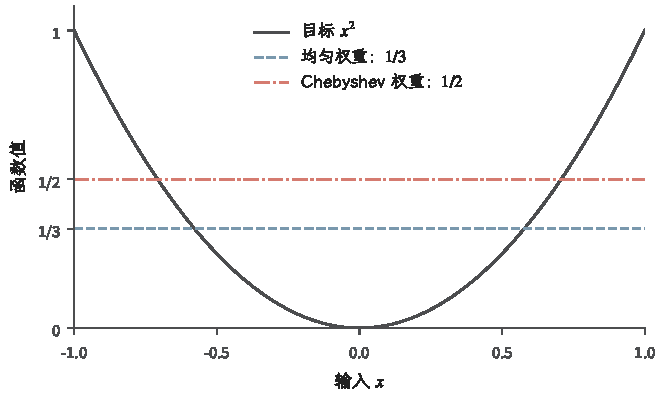
\includegraphics[width=\linewidth]{figures/math-preparation/concept-revision-analysis-functional/weighted-projection.pdf}
 \caption{对$x^2$使用同一候选空间$\operatorname{span}\{1,x\}$，均匀权重的最佳常数为$1/3$，Chebyshev权重的最佳常数为$1/2$。目标、区间和候选空间保持相同，只改变误差积分的权重。曲线由解析式生成。}
 \label{fig:functional-weighted-projection}
\end{figure}

区间或权重改变后，正交系数必须随之重算。把$[a,b]$仿射映射到$[-1,1]$可以迁移
Legendre或Chebyshev基，但Jacobian因子和权重也会改变。Chebyshev多项式还具有适合
一致逼近与插值的极值分布；这不意味着其加权$L^2$投影自动就是一致范数下的最佳逼近。
投影结论始终相对于所选内积成立，误差度量一旦改变，最佳函数也可能改变。

\subsection{稳定读取与内积表示}

对函数取加权积分、读出一个系数或在一点求值，都会把整条函数变成一个数。要判断这些
读取操作是否稳定，需检查输入函数的小范数误差能否控制输出误差。
\begin{definition}[有界线性泛函]
\label{def:functional-bounded-linear-functional}
设$\mathcal V$为实赋范空间。线性泛函是线性映射$L:\mathcal V\to\mathbb R$。
若存在有限常数$C\geq0$，使
$|L(f)|\leq C\lVert f\rVert_{\mathcal V}$对所有$f\in\mathcal V$成立，则称$L$有界。
\end{definition}
有界不是要求$L$在整个空间中的输出有统一上限，而是要求输出大小相对于输入范数有
统一上限。线性性使$|L(f)-L(g)|\leq C\lVert f-g\rVert$；在赋范空间上，线性泛函
的有界性与连续性等价。Hilbert空间的内积给出一类直接的有界泛函：
$L_h(f)=\langle f,h\rangle_{\mathcal{H}}$。Riesz表示定理说明没有别的有界线性
泛函\scite{math-conway1990functional}

\begin{theorem}[Riesz表示定理]
\label{thm:functional-riesz-representation}
设$\mathcal{H}$为实Hilbert空间。对每个有界线性泛函
$L:\mathcal{H}\to\mathbb{R}$，存在唯一的$h_L\in\mathcal{H}$，使
\begin{equation}
  L(f)=\langle f,h_L\rangle_{\mathcal{H}},
  \qquad f\in\mathcal{H}.
  \label{eq:functional-riesz-representation}
\end{equation}
并且$\lVert L\rVert=\lVert h_L\rVert_{\mathcal{H}}$，其中
$\lVert L\rVert=\sup_{\lVert f\rVert_{\mathcal{H}}\leq1}|L(f)|$。
\end{theorem}

\begin{proof}
若$L=0$，取$h_L=0$即可。以下设$L\neq0$。核空间
$M=\ker L=\{f:L(f)=0\}$是线性子空间；由于$L$连续，$M$也是闭集。选取
$u\in\mathcal{H}$使$L(u)\neq0$。由定理
\ref{thm:functional-hilbert-projection}，可以把$u$唯一分解为
\[
  u=P_Mu+v,\qquad v\in M^\perp.
\]
若$v=0$，则$u\in M$，与$L(u)\neq0$矛盾，故$v\neq0$。
又因$P_Mu\in M=\ker L$，
\[
  L(v)=L(u)-L(P_Mu)=L(u)\neq0,
\]
所以下面的除法合法。

对任意$f\in\mathcal{H}$，向量
\[
  f-\frac{L(f)}{L(v)}v
\]
的$L$值为零，因而属于$M$。它与$v\in M^\perp$正交，所以
\[
  0
  =
  \left\langle
    f-\frac{L(f)}{L(v)}v,v
  \right\rangle_{\mathcal{H}}
  =
  \langle f,v\rangle_{\mathcal{H}}
  -
  \frac{L(f)}{L(v)}\lVert v\rVert_{\mathcal{H}}^2.
\]
整理得到
\[
  L(f)
  =
  \left\langle
    f,\frac{L(v)}{\lVert v\rVert_{\mathcal{H}}^2}v
  \right\rangle_{\mathcal{H}}.
\]
因此可取
$h_L=L(v)v/\lVert v\rVert_{\mathcal{H}}^2$。

若$h_1,h_2$都表示$L$，则
$\langle f,h_1-h_2\rangle=0$对每个$f$成立。取$f=h_1-h_2$便得
$h_1=h_2$。Cauchy--Schwarz不等式给出
$|L(f)|\leq\lVert f\rVert\lVert h_L\rVert$，所以
$\lVert L\rVert\leq\lVert h_L\rVert$；当$h_L\neq0$时取
$f=h_L/\lVert h_L\rVert$得到反向不等式。$h_L=0$的情形也直接成立。
\end{proof}

有时读取结果仍是一个函数，例如把一个函数空间映入另一个函数空间。
此时要比较输出与某个测试方向的内积，就需要把这个测试方向拉回输入空间。
\begin{definition}[Hilbert空间之间的伴随算子]
\label{def:functional-adjoint}
设$\mathcal H,\mathcal G$为实Hilbert空间，$S:\mathcal H\to\mathcal G$为有界线性算子，
即存在有限$C\geq0$使$\lVert Sf\rVert_{\mathcal G}\leq C\lVert f\rVert_{\mathcal H}$。
其伴随是满足
\[
 \langle Sf,g\rangle_{\mathcal G}
 =\langle f,S^*g\rangle_{\mathcal H}
 \quad(f\in\mathcal H,\ g\in\mathcal G)
\]
的有界线性算子$S^*:\mathcal G\to\mathcal H$。
\end{definition}
对固定$g$，左边是关于$f$的有界线性泛函，Riesz表示给出唯一的$S^*g$；
表示元的唯一性又保证$S^*$线性，且$\lVert S^*g\rVert_{\mathcal H}\leq C\lVert g\rVert_{\mathcal G}$。
因此伴随确实存在且唯一。它把内积中的算子换到另一侧，并不要求$S$可逆；
有限维实正交坐标中它对应通常的转置；复内积空间使用相应的复数版本，才对应共轭转置。后面的Mercer证明会对空间之间的
包含映射使用同一概念。

\section{正定核与再生核空间}
\label{sec:functional-positive-kernels-rkhs}

整体误差小未必使每个点的函数值接近，前面的尖峰例子已经说明这一点。
若观测和预测通过点值进行，就需要点值读取相对于空间范数稳定。
前节已为一般稳定读取建立Riesz表示；本节专门考察点值泛函，核由此成为空间中的表示对象，
后面的有限核展开则是优化问题在这个空间内的结果。

\subsection{点值泛函与再生核}

上一小节允许读取任意有界线性泛函。这里专门要求读出$f(x)$，因为有限观测与预测通常
需要访问函数在指定位置的值。
\begin{definition}[再生核Hilbert空间]
\label{def:functional-rkhs}
设$\mathcal X$为非空集合，$\mathcal H\subseteq\mathbb R^{\mathcal X}$是实值函数
Hilbert空间。若对每个$x\in\mathcal X$，点值泛函$\delta_x(f)=f(x)$均有界，
则称$\mathcal H$为\term{再生核Hilbert空间}。
\end{definition}
定义要求空间元素是真正具有确定点值的函数。不同的$x$可以使用不同的有界常数；
它并没有要求$x\mapsto f(x)$在某种输入拓扑下连续。
Riesz表示定理给出唯一元素$K_x\in\mathcal{H}$，使
\begin{equation}
  f(x)=\langle f,K_x\rangle_{\mathcal{H}},
  \qquad f\in\mathcal{H}.
  \label{eq:functional-reproducing-property}
\end{equation}
定义
\[
  K(x,z)=K_z(x)
  =\langle K_z,K_x\rangle_{\mathcal{H}},
\]
便得到空间的\term{再生核}（reproducing kernel）。式
\eqref{eq:functional-reproducing-property}说明“再生”的含义：函数在$x$处的值可以
由函数与核截面$K_x=K(\,\cdot\,,x)$的内积读出。

普通$L^2(\mu)$通常不是RKHS。其元素是几乎处处等价类，在单个点上改值不改变元素，
所以$f(x)$甚至未必定义良好。即使人为选择代表元，点值也一般不连续：在$[0,1]$上可以
构造支撑越来越窄而在固定点取值为$1$的连续尖峰，其$L^2$范数趋于$0$。因此，从
$L^2$收敛不能推出固定点的函数值收敛。RKHS范数额外控制点值，因为
\begin{equation}
  |f(x)|
  \leq
  \lVert f\rVert_{\mathcal{H}}
  \lVert K_x\rVert_{\mathcal{H}}
  =
  \lVert f\rVert_{\mathcal{H}}\sqrt{K(x,x)}.
  \label{eq:functional-rkhs-pointwise-bound}
\end{equation}

输入之间的核值也不能随意指定：必须让任何有限线性组合的平方长度非负。
\begin{definition}[实正定核]
\label{def:functional-positive-definite-kernel}
设$\mathcal X$非空。对称函数$K:\mathcal X\times\mathcal X\to\mathbb R$若对每个
$n\geq1$、任意$x_1,\ldots,x_n\in\mathcal X$和$a_1,\ldots,a_n\in\mathbb R$都满足
$\sum_{i,j=1}^n a_i a_jK(x_i,x_j)\geq0$，则称其为\term{正定核}
（positive definite kernel）。本章采用核理论中允许半正定的命名惯例。
\end{definition}
从再生性质得到的核满足这个条件，因为
\begin{equation}
  \sum_{i,j=1}^{n}a_i a_jK(x_i,x_j)
  =
  \left\lVert\sum_{i=1}^{n}a_iK_{x_i}\right\rVert_{\mathcal{H}}^2
  \geq0.
  \label{eq:functional-positive-definite-kernel}
\end{equation}
这里沿用核理论的惯例，“正定”允许有限Gram矩阵奇异；若非零系数和互异输入总使二次型
严格为正，才称严格正定。

正定核的一个可直接核验的来源是有限维特征内积。给定映射
$\bm{\phi}:\mathcal{X}\to\mathbb{R}^d$，令
\[
  K_{\bm{\phi}}(x,z)
  =
  \langle\bm{\phi}(x),\bm{\phi}(z)\rangle_2.
\]
对任意有限输入与实系数，
\[
  \sum_{i,j=1}^{n}a_i a_jK_{\bm{\phi}}(x_i,x_j)
  =
  \left\lVert
    \sum_{i=1}^{n}a_i\bm{\phi}(x_i)
  \right\rVert_2^2
  \geq0,
\]
所以$K_{\bm{\phi}}$满足有限半正定条件。例如，当
$\mathcal{X}\subseteq\mathbb{R}$且
$\bm{\phi}(x)=(1,x)^{\top}$时，得到$K_{\bm{\phi}}(x,z)=1+xz$。

\begin{example}[二维函数空间中的再生核]
\label{ex:functional-affine-rkhs}
令$\mathcal X=[-1,1]$，$\mathcal H=\{f(x)=a+bx:a,b\in\mathbb R\}$，
内积为$\langle a+bx,c+dx\rangle=ac+bd$。输入$z$的核截面是
$K_z(x)=1+zx$，因为$\langle a+bx,1+zx\rangle=a+bz=f(z)$。
于是$K(x,z)=1+xz$，$\lVert f\rVert_{\mathcal H}^2=a^2+b^2$，点值上界为
$|f(z)|\leq\sqrt{1+z^2}\sqrt{a^2+b^2}$。

这说明核既可来自有限维空间，也可来自无限维空间。取三个互异输入时，Gram矩阵秩仍至多
为$2$，因为只有两个独立特征方向；核半正定不保证每个有限Gram矩阵都可逆。
表示同一函数的三项核系数可能不唯一，而空间中的函数仍可由严格凸的正则化目标唯一决定。
图~\ref{fig:functional-affine-point-readout}把$f\mapsto f(3/4)$画成系数平面上的读取。
系数圆给出范数上界，平行直线给出相同点值；最远的点值发生在核方向上，
所以点值上界中的$\sqrt{1+z^2}$正是该方向的长度。
\begin{figure}[htbp]
 \centering
 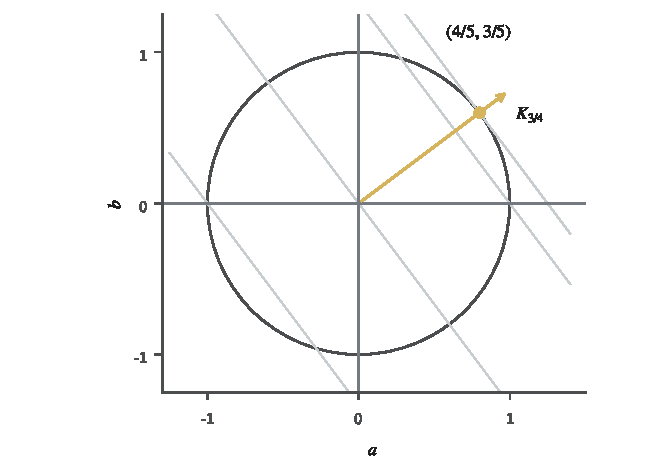
\includegraphics[width=\linewidth]{figures/math-preparation/reader-revision-analysis/functional-affine-point-readout.pdf}
 \caption{仿射RKHS中读取$f(3/4)=a+3b/4$。灰圆表示$a^2+b^2\leq1$，
 黄箭头是核截面$K_{3/4}$对应的系数$(1,3/4)$；灰平行线为相同点值。
 黄圆点$(4/5,3/5)$达到单位范数球上的最大点值$5/4$。这里坐标是函数系数，不是输入位置。图为解析教学示例。}
 \label{fig:functional-affine-point-readout}
\end{figure}

\end{example}

\subsection{Moore--Aronszajn构造}

上面的推导从函数空间得到核。反方向同样成立，而且不需要输入域带有拓扑或测度
\scite{aronszajn1950kernels}

\begin{theorem}[正定核的RKHS构造]
\label{thm:functional-moore-aronszajn-construction}
设$\mathcal{X}$为任意非空集合，$K:\mathcal{X}\times\mathcal{X}\to\mathbb{R}$
对称，并满足式\eqref{eq:functional-positive-definite-kernel}的有限半正定条件。则存在
唯一的函数RKHS $\mathcal{H}_K$以$K$为再生核；这里的唯一性指保持每个函数不变的
等距同构。
\end{theorem}

\begin{proof}
先令$\mathcal{V}_0$为核截面符号$K_x$的形式有限线性组合所成的向量空间：
\[
  \mathcal{V}_0
  =
  \left\{
    \sum_{i=1}^{n}a_iK_{x_i}:
    n\in\mathbb{N},\
    a_i\in\mathbb{R},\
    x_i\in\mathcal{X}
  \right\}.
\]
这里的$K_x$暂时只是由$x$索引的形式符号，尚未把不同形式和按逐点函数值识别。
对
$f=\sum_i a_iK_{x_i}$和$g=\sum_jb_jK_{z_j}$定义
\begin{equation}
  \langle f,g\rangle_0
  =
  \sum_{i,j}a_i b_jK(x_i,z_j).
  \label{eq:functional-kernel-pre-inner-product}
\end{equation}
正定性只保证$\langle f,f\rangle_0\geq0$，还可能有非零形式和的长度为零。令
\[
  \mathcal{N}
  =
  \{f\in\mathcal{V}_0:\langle f,f\rangle_0=0\}.
\]
由半内积的Cauchy--Schwarz不等式，$f\in\mathcal{N}$时
$\langle f,g\rangle_0=0$对所有$g$成立。因此可以商掉$\mathcal{N}$，使式
\eqref{eq:functional-kernel-pre-inner-product}成为真正的内积。

还需证明这个商空间能够忠实地解释为函数。对形式和
$f=\sum_i a_iK_{x_i}$，定义
\[
  (Jf)(x)
  =
  \sum_i a_iK(x,x_i)
  =
  \langle f,K_x\rangle_0.
\]
若$f\in\mathcal{N}$，则
\[
  |(Jf)(x)|^2
  =
  |\langle f,K_x\rangle_0|^2
  \leq
  \langle f,f\rangle_0K(x,x)
  =0,
\]
所以$Jf$处处为零。反过来，若$Jf$处处为零，则
\[
  \langle f,f\rangle_0
  =
  \sum_i a_i(Jf)(x_i)
  =0,
\]
故$f\in\mathcal{N}$。因此$\ker J=\mathcal{N}$，商空间
$\mathcal{H}_0=\mathcal{V}_0/\mathcal{N}$可单射地识别为函数空间，并且其中的
函数满足
\[
  f(x)=\langle f,K_x\rangle_0.
\]

对这个内积空间作完备化，得到Hilbert空间$\mathcal{H}_K$。还要确认完备化后的抽象极限
仍是函数。若$(f_m)\subset\mathcal{H}_0$在核范数下为柯西序列，则对每个$x$，
\[
  |f_m(x)-f_\ell(x)|
  \leq
  \lVert f_m-f_\ell\rVert_0\sqrt{K(x,x)},
\]
所以$(f_m(x))$是实数柯西序列。定义$f(x)=\lim_m f_m(x)$。若另一个柯西序列与
$(f_m)$表示同一个完备化元素，同一不等式保证两者逐点极限相同。故完备化元素具有
良定义的函数值，且内积连续性给出
\[
  f(x)
  =
  \lim_m\langle f_m,K_x\rangle_0
  =
  \langle f,K_x\rangle_{\mathcal{H}_K}.
\]
再生性质因此延伸到整个$\mathcal{H}_K$。这个逐点解释在完备化后仍是单射：若
$f\in\mathcal{H}_K$处处取零，则$f$与每个$K_x$正交；核截面的线性张成
$\mathcal{H}_0$在其完备化$\mathcal{H}_K$中稠密，所以$f$与整个空间正交，只能有
$f=0$。

唯一性也由这个构造确定。若另一个RKHS $\widetilde{\mathcal{H}}$也以$K$为核，则有限核截面和
在两个空间中的内积都由式
\eqref{eq:functional-kernel-pre-inner-product}决定。核截面的线性张成在任一空间中
都稠密；否则与所有$K_x$正交的函数$f$满足$f(x)=0$对所有$x$成立，只能是零函数。
所以有限核截面和之间的恒等映射唯一地延伸为两个完备空间之间的等距同构。
\end{proof}

定理\ref{thm:functional-moore-aronszajn-construction}说明，验证所有有限Gram矩阵半正定
就足以定义一个RKHS。它不同于Mercer谱展开。后者通常还假设$\mathcal{X}$是紧空间、
$K$连续，并选定具有适当支持的有限测度；这些条件使积分算子
\[
  (T_Kf)(x)
  =
  \int_{\mathcal{X}}K(x,z)f(z)\,\mathrm{d}\mu(z)
\]
成为紧自伴算子，从而可以用特征值与特征函数展开$K$。一般正定核即使不满足这些拓扑和
测度条件，仍有上述RKHS构造。因而，核的合法性、核的谱展开以及谱展开的一致收敛是三项
条件不同的结论。

\subsection{表示定理与有限核展开}

RKHS可能无限维，但许多训练目标只通过有限个点值读取$f$。再生性质使这些读取方向恰好由
有限个核截面表示\scite{scholkopf2001representer}

\begin{theorem}[有限样本表示定理]
\label{thm:functional-representer-theorem}
设$\mathcal{H}_K$是$\mathcal{X}$上的RKHS，训练输入为
$x_1,\ldots,x_n$。令
$\Phi:\mathbb{R}^n\to(-\infty,\infty]$为任意函数，
$\Omega:[0,\infty)\to(-\infty,\infty]$单调不减。考虑
\begin{equation}
  \inf_{f\in\mathcal{H}_K}
  \left\{
    \Phi\bigl(f(x_1),\ldots,f(x_n)\bigr)
    +
    \Omega\bigl(\lVert f\rVert_{\mathcal{H}_K}\bigr)
  \right\}.
  \label{eq:functional-representer-objective}
\end{equation}
若该问题存在最优解，则至少有一个最优解具有形式
\begin{equation}
  f^\star
  =
  \sum_{i=1}^{n}a_iK_{x_i}.
  \label{eq:functional-representer-form}
\end{equation}
若该问题的最优值有限且$\Omega$严格递增，则每个最优解都具有式
\eqref{eq:functional-representer-form}的形式。
\end{theorem}

\begin{proof}
记$M=\operatorname{span}\{K_{x_1},\ldots,K_{x_n}\}$。这是有限维子空间，因而闭。
由投影定理，任意$f\in\mathcal{H}_K$都可唯一分解为
\[
  f=f_M+f_{\perp},\qquad f_M\in M,\quad f_{\perp}\perp M.
\]
对每个训练输入$x_i$，再生性质给出
\[
  f(x_i)
  =
  \langle f_M,K_{x_i}\rangle
  +
  \langle f_{\perp},K_{x_i}\rangle
  =
  f_M(x_i).
\]
因此经验项$\Phi$无法区分$f$与$f_M$。另一方面，正交分解给出
\[
  \lVert f\rVert_{\mathcal{H}_K}^2
  =
  \lVert f_M\rVert_{\mathcal{H}_K}^2
  +
  \lVert f_{\perp}\rVert_{\mathcal{H}_K}^2,
\]
故$\lVert f_M\rVert\leq\lVert f\rVert$。当$\Omega$单调不减时，用$f_M$替换$f$
不会增大目标值。若原问题存在最优解，对任一最优解作此替换便得到$M$中的最优解，也就是
式\eqref{eq:functional-representer-form}。

若最优值有限、$\Omega$严格递增且$f_{\perp}\neq0$，则
$\lVert f_M\rVert<\lVert f\rVert$，经验项不变而惩罚项严格减小，与$f$最优矛盾。
这里最优目标值有限保证经验项与惩罚项都是有限值，因而惩罚项的严格下降确实使总目标
严格下降。
所以每个最优解都必须满足$f_{\perp}=0$。
\end{proof}

定理没有证明式\eqref{eq:functional-representer-objective}必定达到下确界。存在性仍要
由目标的下半连续性、强制性、闭性或其他条件另行保证。它也没有保证系数向量
$(a_1,\ldots,a_n)^{\top}$唯一；若Gram矩阵奇异，不同系数可能表示同一个函数。
单调不减惩罚只保证存在一个有限展开最优解；只有当最优值有限且惩罚严格递增时，才能
排除每个最优解中的非零正交余项。若损失还依赖导数、积分或训练点之外的其他有界线性
泛函，表示空间应加入这些泛函的Riesz表示元，不能仍机械地只写训练点核截面。

\section{核的谱坐标与尺度化正则}
\label{sec:functional-kernel-spectrum-regularization}
再生核与有限表示定理回答点值如何读取、训练目标可在哪些方向中求解。
若想比较整个输入空间中的方向，则还需选测度，把核变成积分算子；
算子的谱坐标随后解释正则化如何逐方向收缩。此处处理的是全域表示与尺度，不是有限Gram矩阵的改名。

\subsection{积分算子与谱结构}

核的谱不是由某个有限Gram矩阵直接定义的。给定测度空间
$(\mathcal{X},\mu)$，假设$\mu$为$\sigma$有限测度；给定可测核$K$，先在$L^2(\mu)$上定义积分算子
\begin{equation}
  (T_Kf)(x)
  =
  \int_{\mathcal{X}}K(x,z)f(z)\,\mathrm{d}\mu(z).
  \label{eq:functional-kernel-integral-operator}
\end{equation}
定义积分式还不够：它必须把空间内的函数送回空间，并且不能任意放大误差。
定义~\ref{def:functional-adjoint}中的有界性提供这种控制；谱展开还需要以下结构。
\begin{definition}[自伴、正与紧算子]
\label{def:functional-operator-properties}
设$T:\mathcal H\to\mathcal H$为实Hilbert空间上的有界线性算子。若对所有$f,g\in\mathcal H$
有$\langle Tf,g\rangle=\langle f,Tg\rangle$，称$T$自伴，即$T^*=T$。
若$T$自伴且$\langle Tf,f\rangle\geq0$对每个$f\in\mathcal H$成立，称$T$为正算子。
若对每个有界序列$(f_n)$，序列$(Tf_n)$都具有在$\mathcal H$中范数收敛的子列，称$T$为紧算子。
\end{definition}
有界性只控制输出大小，紧性还要求输出序列能抽出稳定的近似方向。在无限维
$\ell^2$中，恒等算子有界、自伴且为正，却不紧：前文的单位向量序列经过它仍然
两两相距$\sqrt2$，没有收敛子列。后面的有限秩逼近正是建立紧性的途径。

若$K\in L^2(\mu\otimes\mu)$，Cauchy--Schwarz不等式给出
$\lVert T_K\rVert_{\mathrm{op}}\leq\lVert K\rVert_{L^2(\mu\otimes\mu)}$，且
$T_K$是紧算子。后一个结论可由简单核逼近看出：把$K$在
$L^2(\mu\otimes\mu)$中用有限个矩形指示函数的线性组合逼近，相应积分算子只有有限维
值域；核的$L^2$逼近又控制算子范数误差，所以$T_K$是有限秩算子的范数极限。对称核使
$T_K$自伴，核的有限半正定条件在积分有定义时使$T_K$为正算子。

这里用“特征方向”表示非零向量$h$满足$Th=\lambda h$；
对应的特征值$\lambda$说明沿这个方向被缩放多少。零特征值方向属于$\ker T$，不能用正特征值倒数处理。
紧自伴谱定理说明，$T_K$的非零谱由有限重数的实特征值组成；若非零特征值无限多，它们
只能聚集到$0$。相应特征向量与零空间的闭线性张成等于整个Hilbert空间；换言之，一般
元素由这些方向的正交级数在Hilbert范数下收敛得到。这个结论给出$L^2(\mu)$中的算子谱，
却还没有保证核本身在每个$(x,z)$处都等于特征函数级数
\scite{math-conway1990functional}

\subsection{Mercer展开与全域一致性}

Mercer定理补上点态展开所需的条件。有限Gram矩阵$[K(x_i,x_j)]_{i,j}$只记录有限个输入之间的关系；
积分算子的谱则依赖整个输入空间及其测度。要把后者变成处处成立的连续函数展开，
还必须保证测度没有忽略一个非空开区域。
这里“可分空间”指存在可数稠密子集；紧度量空间的可分性使下面的展开可以用一个可数序列
记录，而非假设所有无限维空间天然都有可数基。

\begin{theorem}[连续正定核的Mercer展开]
\label{thm:functional-mercer}
设$\mathcal{X}$为非空紧度量空间，$\mu$为有限、全支撑Borel测度，即每个非空开集
都有正测度。设$K:\mathcal{X}\times\mathcal{X}\to\mathbb{R}$连续、对称，且对任意
有限输入组满足正定核的半正定条件。则$T_K$是$L^2(\mu)$上的紧、自伴、正算子。
其正特征值按重数记为$(\mu_j)$，可为有限个或可数无穷个；相应特征函数可选为连续的
$L^2(\mu)$标准正交函数$(\psi_j)$，并有
\begin{equation}
 K(x,z)=\sum_{j:\mu_j>0}\mu_j\psi_j(x)\psi_j(z).
 \label{eq:functional-mercer-expansion}
\end{equation}
级数在$\mathcal{X}\times\mathcal{X}$上绝对且一致收敛，且
$\sum_j\mu_j=\int K(x,x)\,\mathrm d\mu(x)<\infty$。
若$K\equiv0$，右侧为空和。$T_K$可能另有零空间，零特征值不进入这个展开。
\end{theorem}

\begin{proof}
证明的关键是先在RKHS中分解，再用连续性把逐点结论加强为一致结论。
由前面的Moore--Aronszajn构造得到$\mathcal H_K$。核连续意味着
\[
 \lVert K_x-K_z\rVert_{\mathcal H_K}^2
 =K(x,x)+K(z,z)-2K(x,z)\longrightarrow0\quad(z\to x),
\]
所以每个$f\in\mathcal H_K$连续。紧度量空间有可数稠密子集，其核截面的张成在
$\mathcal H_K$中稠密，故该空间可分；这使下面的标准正交基和级数可以按可数指标列出。

令$S:\mathcal H_K\to L^2(\mu)$为包含映射$Sf=f$。点值上界保证
$\lVert Sf\rVert_{L^2}^2\leq\lVert f\rVert_{\mathcal H_K}^2\int K(x,x)\,\mathrm d\mu(x)$。
若$Sf=0$，连续函数$f$几乎处处为零；全支撑性排除了非零连续函数只在一个零测开区域
出现的可能，故$f=0$，即$S$单射。取$\mathcal H_K$的标准正交基$(e_j)$，再生性质和
Parseval等式给出
\[
 \begin{aligned}
 \sum_j\lVert Se_j\rVert_{L^2}^2
 &=\int\sum_j|e_j(x)|^2\,\mathrm d\mu(x)\\
 &=\int\lVert K_x\rVert_{\mathcal H_K}^2\,\mathrm d\mu(x)
 =\int K(x,x)\,\mathrm d\mu(x)<\infty.
 \end{aligned}
\]
非负积分与求和的交换由单调收敛保证。这一有限尾和可以直接控制有限秩逼近：
将输入投影到前$N$个基方向所得的有限秩算子逼近$S$，算子范数误差平方不超过上述级数
的尾和，所以$S$紧。

用Riesz表示定义伴随$S^*$。由再生性质核对内积可得$SS^*=T_K$。
紧正算子$S^*S$没有零特征方向，故其标准正交特征向量$(h_j)$构成
$\mathcal H_K$的基。设相应正特征值为$\mu_j$，令
$\psi_j=Sh_j/\sqrt{\mu_j}$。于是$\psi_j$连续且在$L^2(\mu)$中标准正交，
$T_K\psi_j=\mu_j\psi_j$。反向地，$T_K$的任意正特征方向通过$S^*$对应到
$S^*S$的同特征值方向，所以没有遗漏正特征值。对$K_x,K_z$在$(h_j)$中应用Parseval等式，得到
\[
 K(x,z)=\sum_j h_j(x)h_j(z)
       =\sum_j\mu_j\psi_j(x)\psi_j(z).
\]
特别地，对角展开的余项
$r_N(x)=K(x,x)-\sum_{j\leq N}\mu_j\psi_j(x)^2$连续、非负，并逐点单调降到零。
给定$\varepsilon>0$，开集$\{x:r_N(x)<\varepsilon\}$随$N$增加，且覆盖紧空间；
有限子覆盖保证某一个$N$已覆盖全部空间，因此$r_N$一致趋于零。Cauchy--Schwarz
不等式进一步给出
\[
 \sum_{j>N}|\mu_j\psi_j(x)\psi_j(z)|
 \leq\sqrt{r_N(x)r_N(z)}\longrightarrow0
 \quad\text{一致于 }(x,z).
\]
这同时证明绝对收敛及一致收敛。对对角展开积分并用标准正交性，可得
$\int K(x,x)\,\mathrm d\mu(x)=\sum_j\mu_j$。零核的情形直接成立。
\end{proof}

上述证明把两项条件的作用分开了：全支撑性保证连续函数的$L^2$等价类没有隐藏的非零区域，
紧致性将连续的递减余项从逐点控制提升为统一控制。紧自伴算子谱、Mercer点态展开与有限
Gram矩阵分解因此是三个层次的结论，不能仅从有限矩阵的半正定性推断全域的一致展开
\scite{mercer1909functions}

\subsection{谱惩罚与有效维度}

在上述Mercer条件下，$\mu_j>0$的方向构成相应RKHS的谱坐标。函数可写成
$f=\sum_jb_j\psi_j$，其范数为
\begin{equation}
  \lVert f\rVert_{\mathcal{H}_K}^2
  =
  \sum_{j:\mu_j>0}\frac{b_j^2}{\mu_j}.
  \label{eq:functional-rkhs-spectral-norm}
\end{equation}
小特征值方向受到更强惩罚。若$\mu_j$迅速衰减，固定半径的函数难以在高编号方向上拥有
大系数；若谱衰减缓慢，则更多方向能够自由变化。

谱表达还能直接展示二次正则化怎样收缩不同方向。设目标
$y=\sum_{j:\mu_j>0}c_j\psi_j$位于正特征方向的闭张成空间，考虑
\[
  \min_{f\in\mathcal{H}_K}
  \left\{
    \lVert f-y\rVert_{L^2(\mu)}^2
    +
    \lambda\lVert f\rVert_{\mathcal{H}_K}^2
  \right\},
  \qquad \lambda>0.
\]
写$f=\sum_jb_j\psi_j$后，各方向彼此分离，最优系数为
\begin{equation}
  b_j^\star
  =
  \frac{\mu_j}{\mu_j+\lambda}c_j.
  \label{eq:functional-spectral-shrinkage}
\end{equation}
特征值远小于$\lambda$的方向被强烈收缩，特征值远大于$\lambda$的方向则大体保留。
这与第\ref{chap:optimization}章的二次正则化是同一逐方向机制；定理
\ref{thm:functional-representer-theorem}的有限表示处理训练点目标，这里的谱解则
处理总体$L^2(\mu)$目标，两者不能省略各自的存在条件而互相替代。

\begin{figure}[htbp]
 \centering
 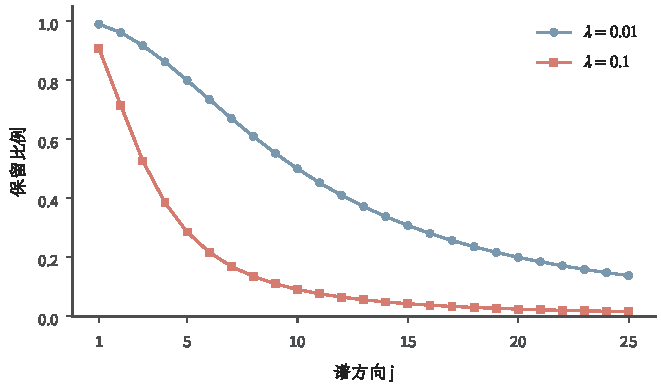
\includegraphics[width=\linewidth]{figures/math-preparation/analysis-geometry/functional-spectral-shrinkage.pdf}
 \caption{教学谱$\mu_j=j^{-2}$上的收缩比例$\mu_j/(\mu_j+\lambda)$。蓝、红线使用$\lambda=0.01$和$0.1$，点标出前$25$个方向；增大正则化后更多方向被抑制。有效维度的定义仍对全部谱方向求和。}
 \label{fig:functional-spectral-shrinkage}
\end{figure}

矩阵迹汇总有限个方向的贡献；无限维空间中的方向可能有无穷多个，因此还要核对这份
总量是否有限。下面把算子条件与所选正则化尺度分开。
\begin{definition}[迹类条件与有效维度]
\label{def:functional-trace-effective-dimension}
设$A$为Hilbert空间上的紧线性算子。$A^*A$的正特征值开方后得到奇异值$s_j(A)$，
按重数排列；若只有有限个，可在其后补零。若$\sum_j s_j(A)<\infty$，称$A$为
\term{迹类算子}（trace-class operator）。对正算子，这等价于非负特征值之和有限，
它的迹就是这个和。

若紧正算子$T_K$的正特征值为$(\mu_j)$，给定$\lambda>0$，其
\term{有效维度}（effective dimension）定义为
\begin{equation}
  d_{\mathrm{eff}}(\lambda)
  =
  \sum_{j\geq1}\frac{\mu_j}{\mu_j+\lambda}
  \label{eq:functional-effective-dimension}
\end{equation}
这里要求右侧级数有限；等价地，
\[
  d_{\mathrm{eff}}(\lambda)
  =
  \operatorname{tr}\bigl(T_K(T_K+\lambda I)^{-1}\bigr)
\]
并要求$T_K(T_K+\lambda I)^{-1}$为迹类。
\end{definition}
迹类要求有限的谱总量，有效维度则先按尺度收缩各方向，再汇总它们的贡献。
在上述Mercer条件下，$\sum_j\mu_j<\infty$，所以
$d_{\mathrm{eff}}(\lambda)\leq\lambda^{-1}\sum_j\mu_j<\infty$。
每个谱方向按其相对于
$\lambda$的大小贡献$0$到$1$之间的量。$\mu_j\gg\lambda$的方向近似贡献$1$，
$\mu_j\ll\lambda$的方向贡献很小。有限样本Gram矩阵也有对应量
\[
  \operatorname{tr}\left(
    \bm{K}(\bm{K}+n\lambda\bm{I}_n)^{-1}
  \right),
\]
但它依赖当前输入与归一化约定，不应和总体积分算子的
$d_{\mathrm{eff}}(\lambda)$混为同一数值。

有效维度不是代数维数。无限维空间在固定$\lambda$下可以有有限有效维度；反过来，一个
有限参数化若参数到函数的映射高度敏感，也可能形成很大的函数集合。参数数量、谱衰减、
导数规则性和范数半径从不同方面描述复杂度。后续核正则化会同时使用谱和范数；神经切线核
只在相应线性化条件下提供这种空间解释，深层网络本身的复杂度不能无条件等同于某个固定核
的有效维度。

\section{逼近能力与表示选择}
\label{sec:functional-approximation-capacity-representation}

\subsection{稠密性与一致逼近}

沿用定义~\ref{def:functional-density}的稠密性，下面不再只判断极限是否存在，
而是寻找能随目标与精度构造出的具体表示。稠密性是一项表示存在性结论：它允许逼近器依赖目标和精度，却
没有说明需要多少参数、怎样找到逼近器，或从有限观测能否识别它。

多项式提供一个基本例子。对$f\in C([0,1])$，定义Bernstein多项式
\begin{equation}
  (B_mf)(x)
  =
  \sum_{j=0}^{m}
  f\left(\frac{j}{m}\right)
  \binom{m}{j}x^j(1-x)^{m-j}.
  \label{eq:functional-bernstein-polynomial}
\end{equation}
权重非负且由二项式定理知其和为$1$，所以$B_mf(x)$是邻近网格函数值的加权平均。

\begin{theorem}[Bernstein逼近定理]
\label{thm:functional-weierstrass-bernstein}
对每个$f\in C([0,1])$，
\[
  \lVert B_mf-f\rVert_{\infty}\longrightarrow0.
\]
因此，多项式在$C([0,1])$的一致范数下稠密。
\end{theorem}

\begin{proof}
连续函数在紧区间上一致连续且有界。记
$M=\lVert f\rVert_{\infty}$。给定$\varepsilon>0$，可取$\delta>0$使
$|u-x|<\delta$时$|f(u)-f(x)|<\varepsilon/2$。

对固定$x$，把式\eqref{eq:functional-bernstein-polynomial}中的权重记为
$w_{m,j}(x)$。除$\sum_jw_{m,j}(x)=1$外，直接对二项式求导可得
\[
  \sum_{j=0}^{m}
  \left(\frac{j}{m}-x\right)^2w_{m,j}(x)
  =
  \frac{x(1-x)}{m}
  \leq\frac{1}{4m}.
\]
将网格点分为
$|j/m-x|<\delta$与$|j/m-x|\geq\delta$两组。近处一组的函数值差小于
$\varepsilon/2$。远处一组的总权重满足
\[
  \sum_{|j/m-x|\geq\delta}w_{m,j}(x)
  \leq
  \frac{1}{\delta^2}
  \sum_{j=0}^{m}
  \left(\frac{j}{m}-x\right)^2w_{m,j}(x)
  \leq\frac{1}{4m\delta^2}.
\]
因此对所有$x\in[0,1]$，
\[
  |B_mf(x)-f(x)|
  \leq
  \frac{\varepsilon}{2}
  +
  2M\frac{1}{4m\delta^2}.
\]
取$m$足够大使第二项不超过$\varepsilon/2$，便得到一致误差不超过
$\varepsilon$。界对所有$x$使用同一个$m$，所以结论是一致收敛。
\end{proof}

证明展示了规则性怎样影响逼近：目标的一致连续性控制近处网格值的变化，二项式权重的二阶
离散矩控制远处权重。如果已知更强的光滑性，可以得到更具体的误差速率；只有连续性时，
定理仍给出存在性，但不承诺对所有连续函数共享一个与目标无关的快速速率。

多项式同时调整全域系数，分段线性样条则把改动限制在少数相邻区间。设
$a=x_0<x_1<\cdots<x_m=b$，最大网格宽度为
$h=\max_j(x_{j+1}-x_j)$，并令$S_hf$在结点处等于$f$、在每个小区间上线性插值。
若$\omega_f(h)=\sup_{|x-z|\leq h}|f(x)-f(z)|$是$f$的连续模，则
\[
  \lVert f-S_hf\rVert_\infty\leq\omega_f(h).
\]
这是因为区间内的插值值是两个端点函数值的凸组合，每个端点距当前点都不超过$h$。
当$f$二阶连续可微时，Taylor余项进一步给出
\[
  \lVert f-S_hf\rVert_\infty
  \leq
  \frac{h^2}{8}\lVert f''\rVert_\infty.
\]
前一个界只依赖连续性，后一个界用更强规则性换取二阶误差。在固定结点位置时，改变一个样条结点的函数值只改变相邻
片段，而改变一个全局多项式系数通常会影响整个区间；这是局部表示与全局表示的结构差别，
不是两种误差范数之间的优劣结论。
为看清“一个局部改动”的范围，图~\ref{fig:functional-basis-locality}固定同一个中心，
只增加一个单位系数。样条帽函数在相邻结点外严格为零；Bernstein基在整个开区间内非零；
高斯基虽快速衰减，仍在所有位置非零。局部性需要由基函数的支撑或衰减式判断，不能由参数个数判断。
\begin{figure}[htbp]
 \centering
 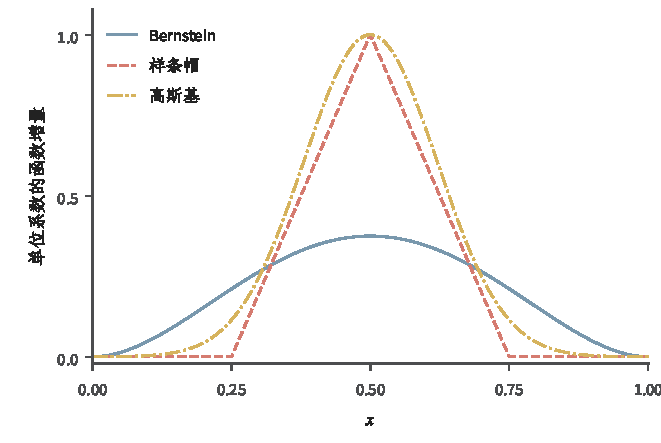
\includegraphics[width=\linewidth]{figures/math-preparation/reader-revision-analysis/functional-basis-locality.pdf}
 \caption{单个系数改变对函数的影响。蓝线为$6x^2(1-x)^2$，即四阶Bernstein多项式的中心基；
 红线为中心$1/2$、相邻结点$1/4,3/4$的线性样条帽；黄线为中心$1/2$、宽度$0.12$的高斯基。
 系数增量均为$1$，不另行缩放峰高；图比较作用范围，未比较三种方法的最优逼近误差。}
 \label{fig:functional-basis-locality}
\end{figure}


\subsection{多项式、样条、核展开与神经网络}

固定目标
\[
  f_\star(x)=\left|x-\frac12\right|,
  \qquad x\in[0,1],
\]
可以看清表示选择的差异。全局多项式用一组遍及整个区间的基函数逼近折点；分段线性样条
只需把$1/2$设为结点，就能精确表示$f_\star$。使用宽度$\sigma>0$的高斯核
\[
  K_\sigma(x,z)
  =
  \exp\left(-\frac{(x-z)^2}{2\sigma^2}\right)
\]
时，可以由若干主要作用于中心附近的核截面$K_\sigma(\,\cdot\,,x_i)$组合出平滑逼近。
高斯核离开中心后衰减，却没有紧支撑；“局部”不表示中心以外恰好为零。有限组合仍是
光滑函数，不能在有限核宽度下精确产生折点。带ReLU激活的单隐藏层网络则可直接写成
\[
  f_\star(x)
  =
  \operatorname{ReLU}\left(x-\frac12\right)
  +
  \operatorname{ReLU}\left(\frac12-x\right).
\]
这些差别来自表示与目标规则性的匹配，不能只由“哪一类更通用”判断。

\begin{table*}[htbp]
 \centering\small
 \begin{tabularx}{\linewidth}{@{}lXX@{}}
 \toprule
 表示 & 对$f_\star(x)=|x-1/2|$的有限表示 & 调整的范围\\
 \midrule
 全局多项式 & 可逼近，有限次数不能精确产生折点 & 一个系数通常影响整个区间\\
 分段线性样条 & 将$1/2$设为结点即可精确表示 & 结点邻域内的分段变化\\
 固定正宽度的高斯核有限和 & 保持光滑，可逼近但不能精确产生折点 & 核中心附近的变化，宽度决定影响范围\\
 两个ReLU单元 & 上式直接给出精确表示 & 隐藏单元的位置和方向决定折点\\
 \bottomrule
 \end{tabularx}
 \caption{同一个连续目标的不同表示。有限表示的结构与整个表示族的稠密性是不同问题。}
 \label{tab:functional-representation-comparison}
\end{table*}

网络表示的逼近能力也需要写清激活条件。仅仅“含非线性”还不够：若
$\sigma(t)=t^2$，所有单隐层有限和仍是次数至多为$2$的多项式，无论增加多少单元都不能
得到任意高次目标。下面的结论允许增加宽度，并要求隐藏单元具有偏置。

\begin{theorem}[单隐藏层的通用逼近]
\label{thm:functional-universal-approximation}
设$\mathcal X\subseteq\mathbb R^d$为非空紧集，$f:\mathcal X\to\mathbb R$连续，
$\sigma:\mathbb R\to\mathbb R$连续且不是多项式。对任意$\varepsilon>0$，存在有限
宽度$m$、实数$a_j,b_j,c$以及$\bm w_j\in\mathbb R^d$，使
\begin{equation}
 \begin{aligned}
 g(\bm x)&=c+\sum_{j=1}^m a_j\sigma(\bm w_j^{\top}\bm x+b_j),\\
 \sup_{\bm x\in\mathcal X}|g(\bm x)-f(\bm x)|&<\varepsilon.
 \end{aligned}
 \label{eq:functional-universal-approximation}
\end{equation}
\end{theorem}

这是Leshno等结果在连续激活情形下的表述\scite{leshno1993approximation}
Sigmoid、Tanh与ReLU都满足激活条件；定理不要求处处可微。连续S形激活在两端分别趋于
$0$与$1$，是非多项式条件的一个常见特例。特别地，紧立方体上的有限和
\begin{equation}
 g(\bm x)=\sum_{j=1}^m a_j\sigma(\bm w_j^{\top}\bm x+b_j)
 \label{eq:functional-sigmoidal-network}
\end{equation}
已能一致逼近连续目标。定理证明涉及更一般的函数空间分离与激活的非多项式性质；本章
前面的Bernstein证明提供稠密性的完整构造，折线与ReLU的对应则给出一维网络版本的直接
构造直觉。

宽度$m$是在给定$f$和$\varepsilon$之后选择的。存在某个表示不保证固定宽度足够，
也不保证训练算法找到参数、有限样本足够或紧集之外的外推准确。向量值目标可以逐坐标
使用结论，再合并有限个单元；目标含跳跃时则不能套用连续目标的一致逼近结论。

不同激活与误差空间还有其他普适逼近版本，但每个版本都必须重新写清定义域、目标集合和
激活条件。它们共同的量词形式是
\[
  \forall f\ \forall\varepsilon>0\
  \exists\text{网络规模与参数，使误差小于 }\varepsilon.
\]
这个陈述没有给出以下任何一项无条件保证：所需网络很小，参数能由可承受的计算找到，
训练算法会到达该参数，或者有限样本上的拟合会在新输入上保持准确。多项式的稠密性也有
同样边界。表示存在、参数规模、优化可计算性和统计泛化是四个不同问题。

误差范数同样决定结论。若只要求$L^2$误差小，逼近器可以在小测度区域出现较大尖峰；若
要求一致误差小，则必须同时控制所有输入。若目标定义在非紧域上，还需要指定加权范数、
局部一致收敛或尾部条件。若目标含不连续点，连续逼近器不可能在整个定义域上一致收敛到
目标，却仍可能在$L^p$意义下逼近。讨论“普适”时必须同时写清目标集合、定义域、逼近器
的并集和误差度量。

\section{函数类的方向、幅度与规则性}
\label{sec:functional-class-size-smoothness}

\subsection{范数球与函数幅度}

上一节允许表示规模随精度增加；这保证可以接近目标，却没有限制候选族还能出现哪些变化。
本节分别限制幅度、导数的累计变化，以及双变量关系中可用的方向数。稠密的表示族可能非常大。若允许多项式次数和系数任意增长，它既能逼近平滑趋势，也能产生
快速振荡。实际分析通常固定一个半径$B$，考察范数球
\[
  \mathcal{F}_B
  =
  \{f\in\mathcal{V}:\lVert f\rVert_{\mathcal{V}}\leq B\}.
\]
半径限制只有结合范数含义才有信息。$L^2$范数限制函数整体能量，却不直接限制导数；
下一小节会先把导数定义为积分意义下的对象，再用Sobolev范数同时限制函数值与直到某个
非负整数阶的导数，因而抑制快速振荡。Lipschitz约束
$|f(x)-f(z)|\leq L|x-z|$则直接限制输入变化造成的输出变化。它们控制的对象不同，
不能由一个较小的参数数量替代。

在RKHS中，式\eqref{eq:functional-rkhs-pointwise-bound}说明核对角有界时，核范数球
统一控制点值。两个输入之间还有
\begin{equation}
  |f(x)-f(z)|
  \leq
  \lVert f\rVert_{\mathcal{H}_K}
  \lVert K_x-K_z\rVert_{\mathcal{H}_K},
  \label{eq:functional-rkhs-modulus-bound}
\end{equation}
而
\[
  \lVert K_x-K_z\rVert_{\mathcal{H}_K}^2
  =
  K(x,x)+K(z,z)-2K(x,z).
\]
因此，核既确定可用方向，也确定输入变化在空间中有多远；半径再限制沿这些方向的幅度。
改变核与改变正则化强度不是同一操作。

\subsection{弱导数与Sobolev空间}

经典导数要求逐点极限存在，会排除带尖点但整体仍然规则的函数。为了只保留积分运算真正
需要的变化信息，可以反过来要求分部积分恒等式成立：让导数先作用在光滑测试函数上，
再检验能否由另一个普通函数表示结果。测试函数用来探测局部变化，其紧支撑意味着它在
靠近区域边界处恒为零，因此不会引入边界项。
\begin{definition}[测试函数与局部可积性]
\label{def:functional-tests-local-integrability}
设$U\subseteq\mathbb R^d$开。函数$\varphi$的支撑是集合
$\{\bm x\in U:\varphi(\bm x)\neq0\}$在$\mathbb R^d$中的闭包。
$C_c^\infty(U)$由无限次连续可微、支撑为$U$内紧集的实函数组成。
空间$L^1_{\mathrm{loc}}(U)$由对每个紧集$K\subset U$满足
$\int_K|f|<\infty$的可测函数的几乎处处等价类组成。
\end{definition}
前一项让测试远离边界，后一项让与任何局部测试函数的积分有限；不要求$f$在整个$U$上可积。
\begin{definition}[弱导数]
\label{def:functional-weak-derivative}
设$U\subseteq\mathbb R^d$开，$f\in L^1_{\mathrm{loc}}(U)$。
取多重指标$\alpha=(\alpha_1,\ldots,\alpha_d)\in\mathbb{N}_0^d$，记
$|\alpha|=\sum_{j=1}^d\alpha_j$，
$D^\alpha=\partial_1^{\alpha_1}\cdots\partial_d^{\alpha_d}$。若存在
$g_\alpha\in L^1_{\mathrm{loc}}(U)$使每个
$\varphi\in C_c^\infty(U)$都满足
\begin{equation}
  \int_U f(\bm{x})D^\alpha\varphi(\bm{x})\,\mathrm{d}\bm{x}
  =
  (-1)^{|\alpha|}
  \int_U g_\alpha(\bm{x})\varphi(\bm{x})\,\mathrm{d}\bm{x},
  \label{eq:functional-weak-derivative}
\end{equation}
就称$g_\alpha$为$f$的$\alpha$阶\term{弱导数}（weak derivative），记为
$D^\alpha f$，按几乎处处等价理解。
\end{definition}
式\eqref{eq:functional-weak-derivative}把经典分部积分当作定义；
测试函数的紧支撑使边界项消失，因此这个定义本身不需要给$U$另加边界条件。

有了弱导数，就可以同时累计函数值与导数的平方误差，得到比$L^2$更强的规则性要求。
\begin{definition}[整数阶平方可积Sobolev空间]
\label{def:functional-sobolev-space}
设$U\subseteq\mathbb R^d$为开集，$m\in\mathbb N_0$。Sobolev空间
\[
  W^{m,2}(U)
  =
  \left\{
    f\in L^2(U):
    D^\alpha f\in L^2(U),\ |\alpha|\leq m
  \right\}
\]
配备范数
\begin{equation}
  \lVert f\rVert_{W^{m,2}(U)}^2
  =
  \sum_{|\alpha|\leq m}
  \lVert D^\alpha f\rVert_{L^2(U)}^2.
  \label{eq:functional-sobolev-norm}
\end{equation}
其中$D^0f=f$，所有导数均按弱导数理解，元素按几乎处处等价识别。
\end{definition}
当$U=(a,b)$为一维区间时，$W^{m,2}(a,b)$也常记作$H^m(a,b)$，式
\eqref{eq:functional-sobolev-norm}相应写成
\[
  \lVert f\rVert_{H^m(a,b)}^2
  =
  \sum_{r=0}^{m}
  \int_a^b|D^r f(x)|^2\,\mathrm{d}x.
\]
这里$m\in\mathbb{N}_0$，各阶导数都按上面的弱导数定义理解；非整数阶Sobolev空间需要
其他定义，不由这个有限求和给出。
例如一维函数$f(x)=|x|$在原点没有经典导数，但其一阶弱导数几乎处处等于
$\operatorname{sign}(x)$；在有界区间上，它仍属于$W^{1,2}$。尖点因而不会自动排除
积分意义下的平滑性。

在$(-1,1)$上把积分分成左右两段，可以直接核对这一弱导数：
\[
 \int_{-1}^1 |x|\varphi'(x)\,\mathrm dx
 =\int_{-1}^0\varphi(x)\,\mathrm dx-\int_0^1\varphi(x)\,\mathrm dx
 =-\int_{-1}^1\operatorname{sign}(x)\varphi(x)\,\mathrm dx.
\]
两侧在$0$处的边界项都为零，原点处任意指定的单个导数值也不会改变积分。
图~\ref{fig:functional-weak-derivative}将这两条函数并列：弱导数允许用一个几乎处处
确定的函数保存变化信息，而不要求补出尖点处不存在的经典导数。
\begin{figure*}[htbp]
 \centering
 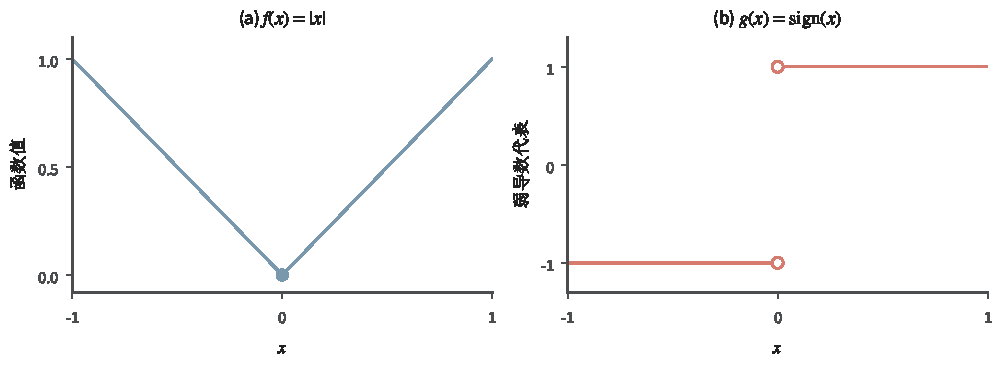
\includegraphics[width=\linewidth]{figures/math-preparation/concept-revision-analysis-functional/weak-derivative.pdf}
 \caption{$f(x)=|x|$与其一阶弱导数$g(x)=\operatorname{sign}(x)$。左图原点为连续尖点；右图两段分别为$-1$与$1$，空心端点表示经典导数在原点未定义。弱导数在原点的代表值可以任取，积分恒等式不受影响。}
 \label{fig:functional-weak-derivative}
\end{figure*}

几乎处处存在经典导数仍不足以保证该导数就是弱导数。阶跃函数
$h(x)=\mathbb I\{x>0\}$几乎处处的经典导数为零，但
$\int_{-1}^1h\varphi'=-\varphi(0)$一般不为零。若能由某个局部可积函数$g$表示
它的弱导数，取支撑逐渐缩到原点、满足$0\leq\varphi_n\leq1$且$\varphi_n(0)=1$的
光滑测试函数，则$|\int g\varphi_n|\to0$，却应等于$1$，矛盾。因此跳跃与连续尖点
在弱导数意义下也有不同表现；单凭“只在一个点不可微”无法判断Sobolev成员资格。

$W^{m,2}(U)$是Hilbert空间。证明完备性时，取其中的柯西列$(f_n)$。对每个
$|\alpha|\leq m$，序列$(D^\alpha f_n)$在$L^2(U)$中都是柯西列，故收敛到某个
$g_\alpha\in L^2(U)$，其中$g_0$记为$f$。把$f_n$的弱导数恒等式分别在两侧取极限；
Cauchy--Schwarz不等式保证与固定测试函数的积分连续，于是
\[
  \int_U fD^\alpha\varphi
  =
  (-1)^{|\alpha|}\int_U g_\alpha\varphi.
\]
因此$g_\alpha=D^\alpha f$，并且$f_n\to f$于
$W^{m,2}(U)$。若另外要求零边界值或其他边界条件，还须证明满足该条件的子空间闭；
一般Sobolev空间的完备性不能替这些边界条件作保证。

\subsection{函数的低秩分解}

前面的表示用基函数、核截面或非线性单元描述一个输入函数。若输入本身分成两组，
还可以利用两组变量之间有限个可分离方向来压缩表示；这就是函数低秩结构的问题。
矩阵的秩在此取本科线性代数中的含义，其系统讨论见第~\ref{chap:linear-algebra}章。
设$p\in\mathcal{P}$表示一种预测或模型索引，
$q\in\mathcal{Q}$表示一种查询、条件或检验索引，量
$E(p,q)\in\mathbb{R}$记录二者组合后的函数值或误差。选取有限对象
$p_1,\ldots,p_m$与$q_1,\ldots,q_n$，可组成矩阵
\[
  \bm{E}_{i,j}=E(p_i,q_j).
\]
若存在映射$\bm{u}:\mathcal{P}\to\mathbb{R}^r$与
$\bm{v}:\mathcal{Q}\to\mathbb{R}^r$使
\begin{equation}
  E(p,q)
  =
  \langle\bm{u}(p),\bm{v}(q)\rangle,
  \label{eq:functional-bilinear-factorization}
\end{equation}
则任意有限矩阵$\bm{E}$的秩至多为$r$。低秩的含义是所有双索引变化都可由$r$个潜在
方向组合，而不是矩阵元素数目少。

Cauchy--Schwarz不等式还把因子尺度传到每个矩阵元素：
\[
  |E(p,q)|
  \leq
  \lVert\bm{u}(p)\rVert_2
  \lVert\bm{v}(q)\rVert_2.
\]
所以秩控制可用方向数，因子范数控制沿这些方向能够产生的幅度。

秩本身只计方向数，不控制数值尺度。若把因子同时变换为
$\bm{u}'(p)=c\bm{u}(p)$和
$\bm{v}'(q)=\bm{v}(q)/c$，式
\eqref{eq:functional-bilinear-factorization}不变，单边因子范数却可以任意改变。
因此，用低秩结构控制误差或计算时，通常还要固定
\[
  \sup_{p\in\mathcal{P}}\lVert\bm{u}(p)\rVert_2\leq B_u,
  \qquad
  \sup_{q\in\mathcal{Q}}\lVert\bm{v}(q)\rVert_2\leq B_v,
\]
或采用对这种缩放更稳定的矩阵范数。方向数$r$与幅度$B_uB_v$承担不同作用。

严格低秩也可能过强。若存在
\[
  E(p,q)
  =
  \langle\bm{u}(p),\bm{v}(q)\rangle+\eta(p,q),
  \qquad
  \sup_{p,q}|\eta(p,q)|\leq\delta,
\]
则$r$描述结构化主项的方向数，$\delta$描述剩余表示误差。增大$r$可能减小$\delta$，
但不会自动给出怎样找到因子、怎样选择查询或怎样由有限观测估计矩阵。代数上的低秩、
因子范数、逼近误差、数据访问条件和计算过程仍须分别说明。

强化学习中的某些复杂度概念会把模型与分布之间的Bellman残差组织成类似矩阵，再研究其
秩或因子化结构。那里的矩阵条目、可实现性、查询协议和样本保证依赖具体决策对象，必须在
相应章节重新定义。仅仅看到某个双线性表达，既不能直接称其为Bellman秩，也不能推出高效
学习。本节提供的是识别这类结构时所需的共同语言。

\section{函数类的覆盖数与度量熵}
\label{sec:functional-combinatorial-metric-complexity}

\subsection{组合模式与距离近似}

第~\ref{chap:combinatorics}章的第~\ref{sec:comb-families-counting}节已经建立
打散、生长函数与组合维度：它们考察有限输入上能独立实现哪些输出选择。本节转向
函数近似，问在指定误差范围内，需要多少个代表函数才能近似整个函数类。
模式是否可实现与近似误差有多大，是两个需要分别说明的问题。

对非空输入空间$\mathcal X$上的非空二值函数类$\mathcal F\subseteq\{0,1\}^{\mathcal X}$及输入组$S=(x_1,\ldots,x_n)$，
沿用组合章的限制类记号和定义~\ref{def:growth-function}：
\begin{equation}
 \mathcal F|_S=\{(f(x_1),\ldots,f(x_n)):f\in\mathcal F\},
 \qquad \Pi_{\mathcal F}(n)\text{表示该类的生长函数}.
 \label{eq:functional-growth-function}
\end{equation}
固定$S$只观察这组输入，生长函数还要在所有$n$个输入的选择之间取最坏情况。
定义~\ref{def:vc-dimension}与引理~\ref{lem:sauer-shelah}提供模式数的组合控制，
但没有为两个函数在整个定义域上的误差选择距离。

例如实线上由$a\in\mathbb R$索引的阈值函数类，
$f_a(x)=\mathbb{I}\{x\geq a\}$，在$n$个互异且有序的输入上只能产生$n+1$种模式，
而全部二值函数可以产生$2^n$种模式。但只要$a\neq b$，就有
$\sup_{x\in\mathbb R}|f_a(x)-f_b(x)|=1$：两个阈值之间总有输入使输出不同。
在固定$n$个输入上模式有限，并不说明另一个阈值函数能在所有输入上提供小于$1$的
最坏误差。前一种比较统计输出模式，后一种比较函数在指定位置上的差值。

有限函数类给出另一个直接的上界。若$\#\mathcal{F}=M<\infty$，每个函数在固定输入组上
至多贡献一种模式，因而
\[
  \Pi_{\mathcal{F}}(n)\leq\min\{M,2^n\}.
\]
例如只含两个常值函数$f_0(x)=0$与$f_1(x)=1$的函数类，在任意非空输入组上恰好产生
全零和全一两种模式，所以$\Pi_{\mathcal{F}}(n)=2$对所有$n\geq1$成立。有限类的函数数目
限制了模式总数，但不同函数在某组输入上可能给出相同限制，因此一般只能得到上界。

实值函数的伪维与胖打散维同样回用组合章第~\ref{sec:comb-real-valued-threshold-margins}节。
伪维检查能否跨过固定阈值，胖打散维还规定阈值两侧的间隔。函数近似则需要另行规定
比较哪些输入、怎样汇总误差：上确界误差关注最坏位置，平方积分误差关注测度加权的
整体差异。选定这种距离后，才能用代表函数的数量描述给定精度下的近似规模。

\subsection{覆盖数与度量熵}

把候选函数逐个列出可能需要无穷多个对象。如果容许误差不超过$\varepsilon$，一组有限
代表却可能已经够用。覆盖数记录的是这组代表至少需要多少个，而不是原类有多少个函数。
\begin{definition}[函数类的覆盖数与度量熵]
\label{def:functional-covering-number}
设$\mathcal F$为非空函数类，$d$为定义~\ref{def:analysis-pseudometric}中的伪距离；
只看有限输入时，两个不同函数的样本距离可能为零。给定正半径$\varepsilon>0$，
若有限集合$\mathcal{C}\subseteq\mathcal{F}$满足：对每个$f\in\mathcal{F}$，存在
$g\in\mathcal{C}$使$d(f,g)\leq\varepsilon$，则$\mathcal{C}$称为
$\varepsilon$-覆盖。最小覆盖大小记为
\[
  N(\varepsilon,\mathcal{F},d),
\]
若不存在有限$\varepsilon$-覆盖，约定$N=+\infty$；其对数称为度量熵。零半径的覆盖也沿用上述约定，
用于下文$L=0$时的复合函数类。覆盖数回答的是：在指定误差尺度下，需要多少个代表函数才能近似整个
函数类。
\end{definition}
无穷函数类在正尺度下仍可能有有限覆盖；缩小容许误差时，覆盖数只能不减。
覆盖球可以互相重叠，也可以伸到函数类之外，但这里的球心必须属于$\mathcal F$。

距离的选择会改变覆盖对象。常见的$d_\infty$用于有界实函数类，
$d_{L^2(\mu)}$用于同一测度$\mu$下的平方可积函数类，而样本距离$d_S$取非空
输入组$S=(x_1,\ldots,x_n)$、$n\geq1$；这些条件保证下列距离有限：
\begin{align*}
  d_{\infty}(f,g)
  &=
  \sup_{x\in\mathcal{X}}|f(x)-g(x)|,\\
  d_{L^2(\mu)}(f,g)
  &=
  \left(
    \int_{\mathcal{X}}|f(x)-g(x)|^2\,\mathrm{d}\mu(x)
  \right)^{1/2},\\
  d_S(f,g)
  &=
  \left(
    \frac1n\sum_{i=1}^{n}|f(x_i)-g(x_i)|^2
  \right)^{1/2}.
\end{align*}
$d_\infty$同时控制所有输入，$d_{L^2(\mu)}$只控制测度$\mu$加权的整体差异，$d_S$
只看给定有限输入。一个样本距离下很小的覆盖未必控制样本外的函数差异；一个
$L^2(\mu)$覆盖也未必控制$\mu$几乎不赋质量的区域。后续概率论章建立随机样本后，
才会讨论怎样把这些确定性覆盖结构接到同时误差概率界。

有限输入上的量化给出一个可以直接核对的覆盖。给定$\varepsilon>0$，设每个$f\in\mathcal{F}$在
$S=(x_1,\ldots,x_n)$上都取值于$[-B,B]$。把该区间分成长度不超过
$\varepsilon$的小区间，并对每个被$\mathcal{F}|_S$占据的$n$维网格单元选取一个
代表函数。落在同一单元的两个函数在每个$x_i$处相差不超过$\varepsilon$，因而其
$d_S$距离也不超过$\varepsilon$。由此得到
\[
  N(\varepsilon,\mathcal{F},d_S)
  \leq
  \left(1+\left\lceil\frac{2B}{\varepsilon}\right\rceil\right)^n.
\]
这个界同时写出了值域$[-B,B]$、分辨率$\varepsilon$和输入数$n$。它只覆盖
$S$上可见的取值向量，不控制其他输入，也不声称该上界达到最小覆盖大小。

图~\ref{fig:functional-covering-centers}把量化的含义放到一个可精确计算的函数族中。
令$f_{a,b}(x)=a+bx$，$a,b\in[-1,1]$，并取$S=(-1,1)$，则
\[
 d_S(f_{a,b},f_{a',b'})^2
 =\tfrac12\bigl((\Delta a-\Delta b)^2+(\Delta a+\Delta b)^2\bigr)
 =(\Delta a)^2+(\Delta b)^2.
\]
因此样本距离恰是系数平面中的欧氏距离。把每个坐标分成三个等宽区间，取九个格心，
就得到半径$\sqrt2/3$的覆盖：任意函数与其格心代表的两项系数差均不超过$1/3$。
这证明$N(\sqrt2/3,\mathcal F,d_S)\leq9$，没有证明九个是最少数量。
\begin{figure}[htbp]
 \centering
 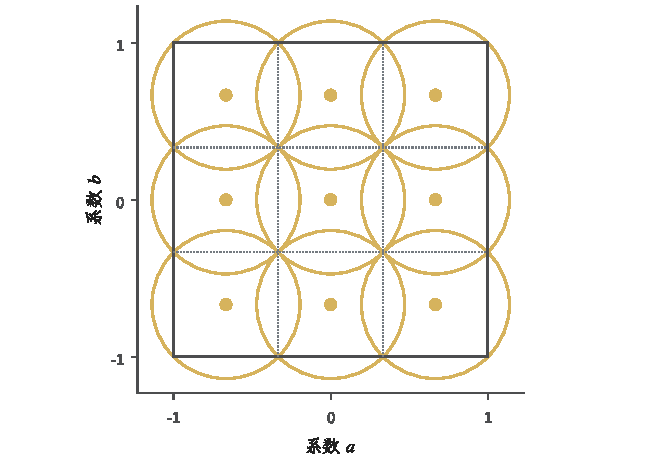
\includegraphics[width=\linewidth]{figures/math-preparation/concept-revision-analysis-functional/covering-centers.pdf}
 \caption{仿射函数族的有限覆盖。方形表示$a,b\in[-1,1]$，九个实心点是类内代表，圆的半径为$\sqrt2/3$。每个小方格都被对应格心的闭球覆盖；圆的重叠与越出方形的部分均不影响覆盖要求。}
 \label{fig:functional-covering-centers}
\end{figure}

覆盖结构还可以由函数类运算传播。若$\mathcal{F}$与$\mathcal{G}$在同一上确界距离下
分别有$\varepsilon_F$与$\varepsilon_G$覆盖，则
\[
  \mathcal{F}+\mathcal{G}
  =
  \{f+g:f\in\mathcal{F},\ g\in\mathcal{G}\}
\]
有半径$\varepsilon_F+\varepsilon_G$、大小至多为两个覆盖大小乘积的覆盖。若
$\varphi:\mathbb{R}\to\mathbb{R}$是$L$-Lipschitz函数，则把
$\mathcal{F}$的$\varepsilon$-覆盖逐点送入$\varphi$，得到
$\varphi\circ\mathcal{F}$的$L\varepsilon$-覆盖。这些关系说明组合结构怎样累积
复杂度，却不自动给出有限样本泛化结论。

覆盖数随距离与误差半径改变，组合维度则随输出区分规则改变。二者都需要明确函数类
与输入对象；把计数界或覆盖界用于学习保证时，还要另加抽样和概率条件。

\section{自适应输入上的函数类复杂度}
\label{sec:functional-sequential-classes-low-rank}

\subsection{查询树与序贯复杂度}

前一节把输入$x_1,\ldots,x_n$预先固定。序贯问题允许第$t$个输入根据此前反馈变化，
单个输入序列因而不能列出所有可能路径。这里用二叉树表达分支，并以
$\epsilon_t\in\{-1,1\}$标记第$t$步选择的分支；$\epsilon_t$只是抽象路径标签，不必
等于实值函数输出$f(\bm{x}_t)$。若具体问题的反馈不是二元值，还需另行给出编码规则或
改用相应的分支集合。
\begin{definition}[二叉查询树]
\label{def:functional-query-tree}
设$\mathcal X$为非空输入集合，$T\geq1$为整数。深度为$T$的\term{查询树}（query tree）由映射
\[
  \bm{x}_t:\{-1,1\}^{t-1}\to\mathcal{X},
  \qquad t=1,\ldots,T,
\]
组成。这里$\{-1,1\}^0$只有空路径，根节点因而是一个固定输入$\bm{x}_1$；在路径
$\bm{\epsilon}=(\epsilon_1,\ldots,\epsilon_T)$上，第$t$步访问
$\bm{x}_t(\epsilon_1,\ldots,\epsilon_{t-1})$。同一个函数$f$沿该路径产生
\[
  \bigl(
    f(\bm{x}_1),
    f(\bm{x}_2(\epsilon_1)),
    \ldots,
    f(\bm{x}_T(\epsilon_1,\ldots,\epsilon_{T-1}))
  \bigr).
\]
\end{definition}
树同时编码所有按过去分支的输入选择规则，本身没有给路径指定概率。

图~\ref{fig:functional-query-tree}只展开两层，便能看见这一信息约束：查询$x_0$之后，
下一次查询取$x_-$还是$x_+$由已出现的分支决定。覆盖中心必须提前为两个可能的下一步
都指定值，不能在分支确定后临时增加一棵新的中心树。
\begin{figure}[htbp]
 \centering
 % Simple three-query tree; centers assign values before a branch is selected.
\begin{tikzpicture}[figure picture,x=1mm,y=1mm,font=\figurefont\footnotesize,
  query/.style={draw=FigureStroke,line width=1pt,rounded corners=1.2mm,
    minimum width=24mm,minimum height=10mm,fill=white,align=center},
  branch/.style={-{Stealth[length=2.2mm,width=1.4mm]},draw=FigureStroke,
    line width=1.1pt,rounded corners=1.2mm}]
 \node[query] (root) at (0,0) {$x_0$};
 \node[query] (left) at (-27,-28) {$x_-$};
 \node[query] (right) at (27,-28) {$x_+$};
 \draw[draw=FigureStroke,line width=1.1pt] (root.south) -- (0,-12);
 \draw[branch] (0,-12) -| (left.north);
 \draw[branch] (0,-12) -| (right.north);
 \node[above,font=\figurefont\footnotesize] at (-16,-12) {$\epsilon_1=-1$};
 \node[above,font=\figurefont\footnotesize] at (16,-12) {$\epsilon_1=+1$};
 \node[right,font=\figurefont\footnotesize,text=FigureInk] at (14,0) {$v_1$};
 \node[below,font=\figurefont\footnotesize,text=FigureInk] at (-27,-35) {$v_2(-1)$};
 \node[below,font=\figurefont\footnotesize,text=FigureInk] at (27,-35) {$v_2(+1)$};
\end{tikzpicture}

 \caption{深度为$2$的固定查询树。根查询$x_0$，左右分支对应$\epsilon_1=-1$与$+1$；下方的$v_1,v_2(\pm1)$是一棵覆盖中心在三个节点预先指定的值，表示近似值而非真实反馈。固定两点输入只观察其中一条路径。}
 \label{fig:functional-query-tree}
\end{figure}

在固定输入上，覆盖中心是一组函数值；在查询树上，它必须为每个可能访问的节点预先
指定一个实数。下面的覆盖条件沿每条路径比较误差，中心集合仍在路径出现之前确定。
\begin{definition}[序贯覆盖与序贯覆盖数]
\label{def:functional-sequential-cover}
给定深度为$T$的查询树$\bm x$、非空实值函数类$\mathcal F$和$\varepsilon>0$。
实数树$v=(v_t)$的每层映射为$v_t:\{-1,1\}^{t-1}\to\mathbb R$。若这些树组成的
有限集合$\mathcal C$满足：对每个$f\in\mathcal F$和每条路径$\bm\epsilon\in\{-1,1\}^T$，
都存在$v\in\mathcal C$使
\begin{equation}
  \left(
    \frac1T\sum_{t=1}^{T}
    \left|
      f\bigl(\bm{x}_t(\epsilon_{1:t-1})\bigr)
      -
      v_t(\epsilon_{1:t-1})
    \right|^2
  \right)^{1/2}
  \leq\varepsilon,
  \label{eq:functional-sequential-cover}
\end{equation}
则称$\mathcal C$为该查询树上的序贯$\varepsilon$-覆盖。其最小大小记为
$N_2^{\mathrm{seq}}(\varepsilon,\mathcal F,\bm x)$；不存在有限覆盖时取$+\infty$。
对所有深度为$T$的查询树取上确界，得到该深度下函数类的序贯覆盖数。
\end{definition}
覆盖集合必须在选择具体函数与路径之前固定，
其中每个$v$都为整棵树的节点赋值，并且第$t$层的值只依赖此前分支
$\epsilon_{1:t-1}$。针对不同的$f$与路径可以从该固定集合中选择不同$v$；不能做的是在
看到完整未来后临时构造一个不属于预定覆盖集合的数值序列。正是这种树形、非前视的中心
保留了序贯信息约束。

序贯覆盖数对所有深度$T$查询树取最坏情形。比较固定输入与查询树之前，必须统一覆盖
中心的约定：上一小节要求中心属于$\mathcal F$，这里的实数树却不必由某个
$f\in\mathcal F$产生。因此在同一半径下，不能直接断言序贯覆盖数更大。例如
$T=1$、$\mathcal F=\{f_-,f_+\}$，其中$f_-\equiv-1$、$f_+\equiv1$，取
$\varepsilon=1$。内部中心的固定覆盖需要两个函数，外部中心$v_1=0$却能同时覆盖二者。

若固定输入的中心也允许是任意实值取值向量，则不分支查询树与这一外部中心覆盖一致，
对所有查询树取最坏情形才保证不小于对所有固定输入取最坏情形。对固定输入上的外部覆盖，若保留内部中心约定，
可在每个被函数类占据的外部$\varepsilon$球中选一个类内代表；三角不等式给出内部
$2\varepsilon$覆盖，数量不增加。这个两倍半径的换算不能省去。反向比较仍需额外规则性。
与胖打散维相似，还可以定义带间隔的序贯打散维；它衡量函数类能否沿树的每条分支持续作出可分辨选择。概率界、
在线遗憾或自适应采样保证还需要后续章节的随机与算法条件，这里只建立输入可适应变化时应
使用的结构对象。

深度为$2$的树已经能展示固定覆盖与序贯覆盖的差别。设根节点查询$x_0$；沿标签
$\epsilon_1=-1$的分支查询$x_-$，沿标签$\epsilon_1=1$的分支查询$x_+$，并假设函数
在这三个点上的值都属于$[-B,B]$。把三个节点值分别量化到宽度不超过$\varepsilon$的
区间，并为
每个被函数类占据的三维网格单元保留一棵代表函数树，就得到序贯
$\varepsilon$-覆盖：左路径比较$(x_0,x_-)$上的两个值，右路径比较
$(x_0,x_+)$上的两个值，每条路径的平方平均误差都不超过$\varepsilon$。固定两点覆盖
只需描述一条已经选定的路径；树覆盖必须在分支发生前同时准备$x_-$与$x_+$处的值。
因此，不能等路径进入某个分支后，再用一个未属于预定覆盖集合的新近似器补上所选分支。

\section{本章小结}
\label{sec:functional-analysis-approximation-summary}

当候选对象从固定长度的系数向量扩展为函数时，必须先说明怎样比较函数。Banach空间用
完备范数容纳逼近极限，Hilbert空间再用内积建立正交与投影。闭凸集投影定理中，凸性与
内积几何先使最小化序列成为柯西列，空间完备性给出极限，集合闭性让极限仍然可行；凸性
还保证最近点唯一。闭子空间上的残差正交由此推广有限维最小二乘。正交系的完备性则是另一
件事，它要求所选方向稠密张成整个空间，不能与Hilbert空间容纳柯西极限的完备性混用。

点值读取不是任意函数空间自动具备的操作。点值泛函有界时，Riesz表示把它变成与核截面的
内积，从而得到RKHS；反过来，任意正定核都能通过有限核截面、零范数商空间与完备化构造
唯一的RKHS。表示定理随后说明，只依赖有限训练点值并配合单调范数惩罚的优化问题，只要
最优解存在，就可在有限核截面张成空间中找到最优解。存在性、系数唯一性和Mercer谱展开
仍各有额外条件，不能由表示形式代替。

函数能够被任意精度逼近，只回答表示存在性。所需规模、求解过程和有限观测下的误差是另外
的问题。范数与平滑性限制函数变化的幅度，谱和有效维度刻画在给定尺度下仍活跃的方向，
组合章的生长函数与胖打散维描述可实现的模式，本章的覆盖数则描述指定距离与分辨率下的
近似规模。输入可以根据过去
变化时，需要用查询树上的序贯结构；双索引关系可由低秩与因子范数描述，但还须单独保留
逼近误差和访问条件。第~\ref{chap:linear-algebra}章将先回到有限维空间，系统建立坐标、
投影、范数与低秩表示；后续第~\ref{chap:probability-theory}章再把平方可积函数的预测
重新解释为条件期望投影，并把这些确定性函数类结构接到有限观测的同时误差控制。


\bookpart{线性和非线性空间}{Linear and Nonlinear Spaces}
\label{part:linear-algebra-and-geometry}

\BookPartGuide{%
本部分研究数据与变换所在的空间。同一个对象可以有不同坐标，坐标差也未必等于实际距离。我们需要空间结构来说明
怎样比较对象、衡量长度和角度，以及局部计算能否揭示整体形状。在线性空间中，
全局基和矩阵提供了统一表示；在非线性空间中，一套全局坐标可能不够用，需要
局部坐标和不随坐标改变的几何量。

第6章“线性空间”围绕向量空间、内积、线性映射和矩阵展开，连接方程求解、谱分解、
低秩近似与扰动分析。矩阵在这里是线性变换的坐标表示；换基、范数和条件数共同决定
数值结果如何解释。第7章“非线性空间与流形”用局部坐标、切空间、度量、联络和曲率
描述弯曲空间，并讨论对称性、拓扑关系及流形上的优化。

两章共享“对象—表示—变换—稳定性”这组问题。线性空间允许用全局基和矩阵统一处理，
流形通常只能在局部线性化；局部切空间能够复用线性工具，却不能代替曲率、拓扑和全局
可达性的判断。}

\chapter{线性空间}
\label{chap:linear-algebra-and-matrix-analysis}
\label{chap:linear-algebra}
\label{chap:matrix-analysis}

同一个线性模型可以提出几种不同的问题：给定参数，怎样得到预测；给定预测，能否反求
参数；反复应用同一个变换，结果怎样变化；只能保留少量方向时，怎样近似原来的作用。
即使这些问题都有精确的数学答案，数据中的微小变化和计算中的舍入仍可能使答案发生
很大变化。因此，矩阵不仅是一张可以相乘的数表，还要连同它表示的空间、几何和任务
一起理解。

本章用一组近共线特征贯穿表示、求解、压缩与误差分析：
\begin{equation}
 \bm X_{\varepsilon}
 =\begin{bmatrix}1&1\\1&1+\varepsilon\\1&1-\varepsilon\end{bmatrix}
 =\begin{bmatrix}\bm c_1&\bm c_2\end{bmatrix},
 \qquad
 \bm q=\begin{bmatrix}0\\1\\-1\end{bmatrix},
 \quad \bm c_2=\bm c_1+\varepsilon\bm q.
 \label{eq:linear-algebra-nearly-collinear-design}
\end{equation}
这里$\bm c_1=(1,1,1)^{\top}$。当$\varepsilon\neq0$时两列线性无关，
但$|\varepsilon|$很小时它们几乎同向，这称为\term{近共线}（nearly collinear）。
“近”指作为输出空间中向量的两列接近同一方向，不是说各个样本点彼此接近。
我们将看到：两列几乎重复时，拟合值可以相当稳定，表示它的两个系数却可能很大。

第~\ref{chap:functional-analysis-and-approximation}章已经建立空间、范数、投影与
伴随的通用语言。本章把它们落实到有限坐标，并依次回答怎样表示变换、反求输入、
计算幂、压缩规模以及判断可靠性。特征分解和奇异值分解各自在需要它们的任务中出现；
反复作用另用一个固定的二维方阵，不对矩形设计矩阵$\bm X_\varepsilon$强行取幂。

\section{线性对象的空间与表示}
\label{sec:linear-algebra-vector-spaces-coordinates}

描述一个对象，需要先确定哪些对象可以相加，再选择记录它的坐标，最后说明怎样比较
两个对象的差异。这三项设定不能互相代替：相同的数值列表可以属于不同空间，同一个
对象可以有不同坐标，而同一个残差在不同几何下也可以有不同大小。

\subsection{线性组合与对象空间}

位移、信号、函数、矩阵都可以作为向量。它们共同的要求是可以做线性组合，而不要求
天然长成一个数字列。设标量域$\mathbb F$为$\mathbb R$或$\mathbb C$。
\term{向量空间}（vector space）$V$对加法和数乘封闭，并满足加法交换律、结合律、
零元与逆元、数乘结合律、两条分配律以及$1\bm v=\bm v$。这些公理保证有限次线性
运算仍有一致的意义。$\mathbb R^d$、所有$m\times d$实矩阵以及次数不超过$k$的
实多项式都是例子；集合$\{\bm x:x_1=1\}$则不是，因为它不包含零向量，也不对加法
封闭。形状像直线并不是线性空间的判据。

非空子集$U\subseteq V$若满足
\[
 a\bm u+b\bm v\in U
 \qquad(\bm u,\bm v\in U,\ a,b\in\mathbb F),
\]
便是\term{线性子空间}（linear subspace）。例如固定形状的有限数组在逐项加法和
数乘下构成空间，满足某些齐次线性约束的数组构成其子空间。经过原点与否在这里很重要：
非零平移后的子空间一般是仿射集合，不再是线性子空间。

给定$\bm v_1,\ldots,\bm v_k$，所有\term{线性组合}（linear combination）
$\sum_j a_j\bm v_j$组成\term{张成空间}（span）
\[
 \operatorname{span}\{\bm v_1,\ldots,\bm v_k\}
 =\left\{\sum_{j=1}^k a_j\bm v_j:a_j\in\mathbb F\right\}.
\]
它是包含这些向量的最小子空间，回答“哪些对象能够表示”。表示是否冗余则由另一个
条件判断：若
\begin{equation}
 a_1\bm v_1+\cdots+a_k\bm v_k=\bm0
 \label{eq:linear-algebra-independence-relation}
\end{equation}
仅在全部$a_j=0$时成立，就称这组向量\term{线性无关}（linearly independent）。
否则挑出一个非零系数并移项，就能把相应向量写成其余向量的线性组合。

在贯穿例中，
\[
 a_1\bm c_1+a_2\bm c_2=(a_1+a_2)\bm c_1+a_2\varepsilon\bm q.
\]
$\bm c_1$与$\bm q$线性无关，所以$\varepsilon\neq0$时两个系数只能都为零；
$\varepsilon=0$时却有$\bm c_1-\bm c_2=\bm0$。因此近共线和线性相关不同：
前者描述接近退化的程度，后者是精确的是非判断。

有限维空间的一组无冗余生成向量称为\term{基}（basis），即同时满足张成和线性无关。
基的向量数为\term{维数}（dimension）$\dim V$。从任一有限生成组中反复删除冗余
成员就能得到基；线性无关组也能逐次加入不在其张成空间中的向量，直至扩充成基。
不同基具有相同大小：若一组有$r$个无关向量，另一组有$s$个生成向量，逐次用前一组
替换后一组中的向量而保持张成，可得$r\leq s$；交换两组又得$s\leq r$。
这一有限维结论支持后面的基扩充和维数计算，不直接推广到无限维函数展开。

有时需要保留一组方向，有时则恰好要忽略它们。前者用子空间表示；后者把沿这些方向
移动后无法区分的对象视为一类。
\begin{definition}[线性空间的商空间]
\label{def:linear-algebra-quotient-space}
设$N$为$V$的线性子空间。规定$\bm x\sim\bm y$当且仅当$\bm x-\bm y\in N$，
等价类$\bm x+N=\{\bm x+\bm n:\bm n\in N\}$组成\term{商空间}（quotient space）
$V/N$，其运算为
\[
 (\bm x+N)+(\bm y+N)=(\bm x+\bm y)+N,\qquad
 a(\bm x+N)=a\bm x+N.
\]
\end{definition}
若换代表元$\bm x'=\bm x+\bm n_1$、$\bm y'=\bm y+\bm n_2$，结果只相差
$\bm n_1+\bm n_2$或$a\bm n_1$，仍属于$N$，所以运算不依赖代表元。
例如$N=\operatorname{span}\{(0,1)^{\top}\}\subset\mathbb R^2$时，每条竖直直线
是一个等价类，商空间只记录第一坐标。取$N$的基并扩充为$V$的基，新增基向量的
等价类构成$V/N$的基，因而$\dim(V/N)=\dim V-\dim N$。求逆时，被变换完全
消去的方向恰好构成这样的$N$。

\subsection{基与坐标组织}
\label{sec:linear-algebra-tensors-structured-operations}

固定有序基$\mathcal B=(\bm b_1,\ldots,\bm b_d)$后，对象$\bm v$唯一写成
$\sum_j x_j\bm b_j$。系数列
$[\bm v]_{\mathcal B}=(x_1,\ldots,x_d)^{\top}$称为\term{坐标}（coordinates）。
存在性来自张成；两组表示相减得到式~\eqref{eq:linear-algebra-independence-relation}，
线性无关性保证唯一性。在$\mathbb R^d$中直接写数字列，通常是默认使用标准基
$\bm e_1,\ldots,\bm e_d$。函数基展开也完全如此：函数是对象，展开系数是坐标。

对象不变时，坐标仍可能很不一样。固定$\delta=0.1$并令
\begin{equation}
 \bm y=\bm c_1+\delta\bm q=\begin{bmatrix}1\\1.1\\0.9\end{bmatrix}.
 \label{eq:linear-algebra-nearly-collinear-target}
\end{equation}
在$\mathcal B_0=(\bm c_1,\bm q)$下坐标是$(1,\delta)^{\top}$。
若$\varepsilon\neq0$，改用同一平面上的基
$\mathcal B_\varepsilon=(\bm c_1,\bm c_2)$，则
\begin{equation}
 \bm y=\left(1-\frac{\delta}{\varepsilon}\right)\bm c_1
       +\frac{\delta}{\varepsilon}\bm c_2.
 \label{eq:linear-algebra-coordinate-instability}
\end{equation}
$\varepsilon=0.01$时坐标成为$(-9,10)^{\top}$，但$\bm y$没有改变。两个很大的
系数在几乎同向的基向量上相消，不能据此判断原对象很大。

若$\mathcal C$是另一组基，把各$\bm b_j$的$\mathcal C$坐标排成列，得到换基矩阵
$\bm S_{\mathcal C\leftarrow\mathcal B}$。保持线性组合给出
\begin{equation}
 [\bm v]_{\mathcal C}
 =\bm S_{\mathcal C\leftarrow\mathcal B}[\bm v]_{\mathcal B}.
 \label{eq:linear-algebra-coordinate-change}
\end{equation}
沿反方向换基能恢复原坐标，两个坐标变换互逆。在上例中
\[
 \bm S_{\mathcal B_0\leftarrow\mathcal B_\varepsilon}
 =\begin{bmatrix}1&1\\0&\varepsilon\end{bmatrix}.
\]
反向求坐标要除以$\varepsilon$，已经提示小扰动可能被放大。此处改变的是记录方式，
不是对对象施加了一个新的物理变换。

多组索引往往比一个很长的坐标列更容易保留语义。
\begin{definition}[多维数值数组]
\label{def:linear-algebra-multidimensional-array}
给定正整数$n_1,\ldots,n_k$，形状为$n_1\times\cdots\times n_k$的数值数组，
是从$\{1,\ldots,n_1\}\times\cdots\times\{1,\ldots,n_k\}$到$\mathbb F$的映射。
第$j$个索引称为第$j$个轴，轴数$k$称为数组的阶。机器学习中常将这样的数组称为
\term{张量}（tensor）。
\end{definition}
例如$\bm X\in\mathbb R^{b\times\ell\times d}$可以记录$b$个样本、每个样本$\ell$个
位置和每个位置$d$个特征；$x_{i,j,k}$由三个索引共同定位。固定部分索引所得对象
称为切片，例如$\bm X_{i,:,:}$保留第$i$个样本，$\bm X_{:,j,k}$保留指定位置、
指定特征在全部样本上的数值。数组阶数是轴数，不是矩阵秩。

\term{维度重排}（permutation of axes）改变轴的顺序。例如
$y_{i,k,j}=x_{i,j,k}$把$b\times\ell\times d$变为$b\times d\times\ell$。
\term{形状重整}（reshape）则先指定元素的遍历顺序，再把同一数列装入另一形状；
仅要求元素总数相同。以
$\bm A=\left[\begin{smallmatrix}1&2&3\\4&5&6\end{smallmatrix}\right]$为例，
轴交换得到
$\bm A^\top=\left[\begin{smallmatrix}1&4\\2&5\\3&6\end{smallmatrix}\right]$，
按行读取后重整成$3\times2$得到
$\left[\begin{smallmatrix}1&2\\3&4\\5&6\end{smallmatrix}\right]$，两者不同。
所以重整不能只给目标形状，还要给顺序。

本章统一用按列堆叠的\term{向量化}（vectorization）：
\[
 \operatorname{vec}(\bm A)
 =(a_{1,1},\ldots,a_{m,1},a_{1,2},\ldots,a_{m,n})^{\top},
 \qquad \bm A\in\mathbb F^{m\times n}.
\]
元素$a_{i,j}$对应索引$i+(j-1)m$。例如上述$\bm A$的向量化为
$(1,4,2,5,3,6)^\top$。这种编码保留全部信息；是否表示输入输出关系，还要看下一节
指定的映射，不能从“它是一张矩阵”直接推出。

数值数组也不自动成为几何中的张量对象。后者还规定各坐标轴怎样随换基共同变换，
使不同分量表代表同一个多线性对象。这里只需要数组及其索引规则；高阶张量分解的
各种秩也不共享矩阵秩的一套结论。区分这些用法，才能避免把存储格式当成几何性质。

\subsection{内积与误差几何}
\label{sec:linear-algebra-length-angle-distance}

坐标确定了怎样记录差异，却没有确定差异的代价。实坐标沿用此前的内积约定
$\langle\bm x,\bm y\rangle=\bm x^\top\bm y$；扩展到复坐标时，本章取
$\langle\bm x,\bm y\rangle=\bm x^*\bm y$，对第一个变量共轭线性、第二个变量线性。
这里$\bm A^*=\overline{\bm A}^{\top}$为共轭转置，实数情形退化为转置。
内积必须共轭对称、正定，并诱导范数
\begin{equation}
 \lVert\bm x\rVert=\sqrt{\langle\bm x,\bm x\rangle}.
 \label{eq:linear-algebra-inner-product-norm}
\end{equation}
零配对表示\term{正交}（orthogonal）。以下回顾两个有限坐标误差界所需的条件。

\begin{theorem}[Cauchy--Schwarz不等式]
\label{thm:linear-algebra-cauchy-schwarz}
在实或复内积空间中，
$|\langle\bm x,\bm y\rangle|\leq\lVert\bm x\rVert\lVert\bm y\rVert$。
等号成立当且仅当两向量线性相关。
\end{theorem}
\begin{proof}
$\bm y=\bm0$时直接成立。否则令
$a=\langle\bm y,\bm x\rangle/\lVert\bm y\rVert^2$，则
\[
 0\leq\lVert\bm x-a\bm y\rVert^2
 =\lVert\bm x\rVert^2-
   \frac{|\langle\bm x,\bm y\rangle|^2}{\lVert\bm y\rVert^2}.
\]
移项即得不等式；等号恰好要求$\bm x=a\bm y$。
\end{proof}

实空间中非零向量的夹角由
$\cos\theta=\langle\bm x,\bm y\rangle/(\lVert\bm x\rVert\lVert\bm y\rVert)$定义；
复内积可能非实，不能直接沿用这一实夹角公式。在贯穿例中
$\bm c_1^\top\bm q=0$、$\lVert\bm c_1\rVert_2^2=3$、
$\lVert\bm c_2\rVert_2^2=3+2\varepsilon^2$，因此
\begin{equation}
 \cos\theta_\varepsilon=\frac{\sqrt3}{\sqrt{3+2\varepsilon^2}}\longrightarrow1.
 \label{eq:linear-algebra-nearly-collinear-angle}
\end{equation}
这给“几乎同向”一个确定的欧氏度量；更换内积也会更换角度。

\term{范数}（norm）满足正定性、绝对齐次性和\term{三角不等式}
（triangle inequality）。有限坐标中常用
\[
 \lVert\bm x\rVert_p=\left(\sum_j|x_j|^p\right)^{1/p}
 \quad(1\leq p<\infty),\qquad
 \lVert\bm x\rVert_\infty=\max_j|x_j|.
\]
它们依次累加绝对偏差、平方偏差或控制最大坐标偏差；距离是差向量的范数
$d(\bm x,\bm y)=\lVert\bm x-\bm y\rVert$。并非每个范数都来自内积。例如
$\ell_1$范数对$\bm e_1,\bm e_2\in\mathbb R^2$使平行四边形恒等式左侧为$8$、
右侧为$4$，不满足式~\eqref{eq:functional-parallelogram-identity}的判据。

\begin{theorem}[有限维Hölder不等式]
\label{thm:linear-algebra-holder}
设$1\leq p,q\leq\infty$且$1/p+1/q=1$，约定$1/\infty=0$。
对于标准坐标配对，
$|\bm x^*\bm y|\leq\lVert\bm x\rVert_p\lVert\bm y\rVert_q$。
\end{theorem}
\begin{proof}
先设$1<p,q<\infty$。Young不等式
$uv\leq u^p/p+v^q/q$对$u,v\geq0$成立：$u>0$时令$t=v/u^{p-1}$，
只需验证$1/p+t^q/q-t\geq0$；其导数为$t^{q-1}-1$，最小值在$t=1$处为零。
$u=0$时也成立。若两向量非零，取
$u_j=|x_j|/\lVert\bm x\rVert_p$、
$v_j=|y_j|/\lVert\bm y\rVert_q$并求和，得到
$\sum_j u_jv_j\leq1/p+1/q=1$。恢复尺度，再用
$|\bm x^*\bm y|\leq\sum_j|x_j||y_j|$即可。零向量时两侧都为零；
$p=1,q=\infty$时用
$\sum_j|x_j||y_j|\leq(\max_j|y_j|)\sum_j|x_j|$，另一端点交换两者。
\end{proof}

Cauchy--Schwarz给出
$\lVert\bm x+\bm y\rVert_2^2\leq(\lVert\bm x\rVert_2+\lVert\bm y\rVert_2)^2$，
从而验证欧氏三角不等式。一般$1<p<\infty$时，将
$|x_j+y_j|^{p-1}$分别与$|x_j|$、$|y_j|$应用Hölder，得到
\[
 \lVert\bm x+\bm y\rVert_p^p
 \leq(\lVert\bm x\rVert_p+\lVert\bm y\rVert_p)
      \lVert\bm x+\bm y\rVert_p^{p-1};
\]
非零时相除，零时直接成立，两个端点逐坐标验证。因此这些表达确实是范数。
有限维范数等价只保证它们给出相同的收敛概念，不保证误差常数相同。例如
\[
 \lVert\bm x\rVert_\infty\leq\lVert\bm x\rVert_2
 \leq\sqrt d\,\lVert\bm x\rVert_\infty,\qquad
 \lVert\bm x\rVert_2\leq\lVert\bm x\rVert_1
 \leq\sqrt d\,\lVert\bm x\rVert_2.
\]
维数增加时$\sqrt d$不能在误差预算中忽略。

若关心的是一次线性读取$\bm z^*\bm r$，最坏误差还取决于读取方向$\bm z$。
\begin{definition}[有限维对偶范数]
\label{def:linear-algebra-dual-norm}
给定$\mathbb F^d$上的范数，相对于标准坐标配对的\term{对偶范数}（dual norm）为
\begin{equation}
 \lVert\bm z\rVert_*=\max_{\lVert\bm r\rVert\leq1}|\bm z^*\bm r|.
 \label{eq:linear-algebra-dual-norm-definition}
\end{equation}
\end{definition}
单位球在有限维中紧，目标连续，故最大值能够达到；它满足范数公理，因为线性读取
满足三角不等式和齐次性，且非零$\bm z$总能读取某个坐标得到非零值。
Hölder给出$\ell_p$单位球上的上界$\lVert\bm z\rVert_q$。当$1<p<\infty$且
$\bm z\neq0$时，取
\[
 r_j=\frac{z_j}{|z_j|}
       \frac{|z_j|^{q-1}}{\lVert\bm z\rVert_q^{q-1}}\quad(z_j\neq0),
 \qquad r_j=0\quad(z_j=0),
\]
就有$\lVert\bm r\rVert_p=1$且$\bm z^*\bm r=\lVert\bm z\rVert_q$。
$p=1$时把单位预算放在$|z_j|$最大的坐标，取相同相位；
$p=\infty$时每个非零坐标都取相同相位。因而
\begin{equation}
 (\lVert\cdot\rVert_p)_*=\lVert\cdot\rVert_q,\qquad \frac1p+\frac1q=1,
 \label{eq:linear-algebra-lp-duality}
\end{equation}
并对$\rho\geq0$有
\begin{equation}
 \max_{\lVert\bm r\rVert_p\leq\rho}|\bm z^*\bm r|
 =\rho\lVert\bm z\rVert_q.
 \label{eq:linear-algebra-linear-perturbation-duality}
\end{equation}
例如$\bm z=(2,-1)^\top$、$|r_j|\leq0.01$时最大变化为$0.03$，
由$\bm r=(0.01,-0.01)^\top$达到。图~\ref{fig:linear-algebra-dual-unit-balls}
固定同一次读取，显示预算形状怎样改变最坏方向。非线性函数若只用此界控制一阶项，
还必须另控余项；这里的对偶范数也不同于第~\ref{sec:opt-duality}节从约束问题构造
下界的拉格朗日对偶。

\begin{figure*}[htbp]
 \centering
 \begin{tikzpicture}[
 x=1mm,y=1mm,font=\figurefont\footnotesize,
 every node/.style={text=FigureInk,inner sep=1pt},
 axis/.style={draw=FigureStroke,line width=.5pt,->},
 boundary/.style={line width=.9pt},
 support/.style={draw=FigureMuted,dashed,line width=.7pt}
]
 \path[use as bounding box] (0,0) rectangle (169,64);
 \node at (25,59) {$\ell_1$：共享绝对值预算};
 \node at (82,59) {$\ell_2$：共享平方预算};
 \node at (139,59) {$\ell_\infty$：逐坐标预算};
 \begin{scope}[shift={(25,30)},x=13mm,y=13mm]
  \draw[axis] (-1.3,0)--(1.55,0) node[right] {$r_1$};
  \draw[axis] (0,-1.3)--(0,1.5) node[above] {$r_2$};
  \draw[boundary,FigureBlue] (1,0)--(0,1)--(-1,0)--(0,-1)--cycle;
  \draw[support] (.35,-1.3)--(1.55,1.1);
  \fill[FigureBlue] (1,0) circle[radius=1.1mm];
  \node[below left] at (0,0) {$0$};
  \node[above left] at (1,0) {$(1,0)$};
 \end{scope}
 \begin{scope}[shift={(82,30)},x=13mm,y=13mm]
  \draw[axis] (-1.3,0)--(1.55,0) node[right] {$r_1$};
  \draw[axis] (0,-1.3)--(0,1.5) node[above] {$r_2$};
  \draw[boundary,FigureRed] (0,0) circle[radius=13mm];
  \draw[support] (.468034,-1.3)--(1.55,.863932);
  \fill[FigureRed] (.894427,-.447214) circle[radius=1.1mm];
  \node[below left] at (0,0) {$0$};
  \node[below left] at (.9,-.48) {$(2,-1)/\sqrt5$};
 \end{scope}
 \begin{scope}[shift={(139,30)},x=13mm,y=13mm]
  \draw[axis] (-1.3,0)--(1.55,0) node[right] {$r_1$};
  \draw[axis] (0,-1.3)--(0,1.5) node[above] {$r_2$};
  \draw[boundary,FigureYellow] (-1,-1) rectangle (1,1);
  \draw[support] (.85,-1.3)--(1.55,.1);
  \fill[FigureYellow] (1,-1) circle[radius=1.1mm];
  \node[below left] at (0,0) {$0$};
  \node[above left] at (1,-1) {$(1,-1)$};
 \end{scope}
 \node at (25,5) {$\max(2r_1-r_2)=2$};
 \node at (82,5) {$\max(2r_1-r_2)=\sqrt5$};
 \node at (139,5) {$\max(2r_1-r_2)=3$};
\end{tikzpicture}

 \caption{同一线性读取$2r_1-r_2$在$\ell_1$、$\ell_2$、$\ell_\infty$单位球上的
 最大值依次为$2$、$\sqrt5$、$3$。虚线为最后接触可行集的支撑直线，点为最大化方向。
 三图坐标尺度相同，均为解析教学例；改变允许误差的形状会改变误差常数。}
 \label{fig:linear-algebra-dual-unit-balls}
\end{figure*}
\FloatBarrier

权重可以进一步区分不同方向的代价。复方阵$\bm M$满足$\bm M^*=\bm M$时称为
Hermitian矩阵，即等于自己的共轭转置；若还对每个非零$\bm x$满足
$\bm x^*\bm M\bm x>0$，则称为Hermitian正定矩阵。这是实对称正定条件的复数对应。
这样的$\bm M$给出
$\langle\bm x,\bm y\rangle_{\bm M}=\bm x^*\bm M\bm y$和
$\lVert\bm x\rVert_{\bm M}=\sqrt{\bm x^*\bm M\bm x}$。
若$\bm M$仅半正定，配对只给半内积，诱导半范数以及
\begin{equation}
 d_{\bm M}(\bm x,\bm y)
 =\sqrt{(\bm x-\bm y)^*\bm M(\bm x-\bm y)}.
 \label{eq:linear-algebra-mahalanobis-pseudodistance}
\end{equation}
半正定的Cauchy--Schwarz仍可从
$\langle\bm x+t\bm y,\bm x+t\bm y\rangle_{\bm M}\geq0$得到，因而三角不等式
保留；不同点的距离却可能为零。这是定义~\ref{def:analysis-pseudometric}的伪距离。
例如$\bm M=\operatorname{diag}(1,0)$无法区分$(0,0)^\top$和$(0,1)^\top$。
后文构造$\bm M=\bm L^*\bm L$后，还能把它写成
$\lVert\bm L(\bm x-\bm y)\rVert_2$：正定时只是改变几何，退化时则消去方向。

对同形矩阵，把元素视为有限坐标，得到Frobenius内积
$\langle\bm A,\bm B\rangle_{\mathrm F}=\sum_{i,j}\overline{a_{i,j}}b_{i,j}$，
以及$\lVert\bm A\rVert_{\mathrm F}=(\sum_{i,j}|a_{i,j}|^2)^{1/2}$。
这是矩阵作为对象的长度；它与矩阵作为变换时的最大放大率并非同一口径。

几何也决定怎样将对象表示到一个较小的子空间。设$U$是有限维内积空间的子空间，
$U^\perp=\{\bm r:\langle\bm u,\bm r\rangle=0,\ \bm u\in U\}$为正交补。
由定理~\ref{thm:functional-hilbert-projection}，有限维闭子空间上存在唯一的
\term{正交投影}（orthogonal projection），将向量分解为
$\bm y=\widehat{\bm y}+\bm r$，其中$\widehat{\bm y}\in U$、$\bm r\in U^\perp$。
对任意$\bm u\in U$，
\[
 \lVert\bm y-\bm u\rVert^2
 =\lVert\bm r\rVert^2+\lVert\widehat{\bm y}-\bm u\rVert^2,
\]
所以投影是唯一最近点\scite{math-axler2015linear}。若$\bm Q$的列为$U$的标准正交基，
$\bm Q^*\bm Q=\bm I$，系数直接由内积读取：
\begin{equation}
 \widehat{\bm y}=\bm Q\bm Q^*\bm y,\qquad
 \bm P_U=\bm Q\bm Q^*,\quad \bm P_U^*=\bm P_U,\quad\bm P_U^2=\bm P_U.
 \label{eq:linear-algebra-orthogonal-projector}
\end{equation}
标准正交基可由逐次减去已有方向的投影并归一化得到，这就是此前的Gram--Schmidt
正交化；减去后为零说明原方向冗余。

一般基不能直接用内积读出坐标，因为基向量之间还会互相贡献。
\begin{definition}[有限向量族的Gram矩阵]
\label{def:linear-algebra-gram-matrix}
向量$\bm b_1,\ldots,\bm b_r$的\term{Gram矩阵}（Gram matrix）为
$g_{i,j}=\langle\bm b_i,\bm b_j\rangle$。若$\bm B$以它们为列，标准坐标中
$\bm G=\bm B^*\bm B$，加权坐标中$\bm G=\bm B^*\bm M\bm B$。
\end{definition}
因为$\bm a^*\bm G\bm a=\lVert\sum_j a_j\bm b_j\rVert^2$，Gram矩阵半正定，
且在内积正定时，正定当且仅当这组向量线性无关。令
$\widehat{\bm y}=\sum_j a_j\bm b_j$，残差与每个$\bm b_i$正交要求
\[
 \sum_j g_{i,j}a_j=\langle\bm b_i,\bm y\rangle.
\]
这给出投影系数的线性方程，而非一组可直接独立读取的坐标。怎样解它，以及方向
冗余时怎样选择系数，留给第~\ref{sec:linear-algebra-reachability-solvability}节。

\begin{example}[同一子空间的两种最近点]
\label{ex:linear-algebra-weighted-projection}
在$\mathbb R^2$中取
\[
 \bm b=(2,1)^\top,\qquad U=\operatorname{span}\{(1,1)^\top\}.
\]
欧氏投影的标量系数满足$2a=3$，故$\bm p=(1.5,1.5)^\top$。
改用$\bm M=\operatorname{diag}(1,4)$，系数满足$5a=6$，得到
$\bm p_{\bm M}=(1.2,1.2)^\top$。第二坐标误差代价更大，最近点便向$b_2=1$靠近。
残差$(0.8,-0.2)^\top$与$(1,1)^\top$的普通内积非零，加权内积却为零。
\end{example}
\begin{figure*}[htbp]
 \centering
 \begin{tikzpicture}[
 x=1mm,y=1mm,font=\figurefont\footnotesize,
 every node/.style={text=FigureInk,inner sep=1pt},
 axis/.style={draw=FigureStroke,line width=.5pt,->},
 vector/.style={line width=.9pt,->}
]
 \path[use as bounding box] (0,0) rectangle (169,65);
 \node at (39,60) {欧氏内积：两坐标等权};
 \node at (123,60) {加权内积：第二坐标权重为 $4$};
 \begin{scope}[shift={(15,10)},x=15mm,y=15mm]
  \draw[axis] (-.15,0)--(3.2,0) node[right] {$x_1$};
  \draw[axis] (0,-.15)--(0,2.8) node[above] {$x_2$};
  \draw[FigureMuted,line width=.7pt] (0,0)--(2.6,2.6)
   node[right] {$U$};
  \draw[vector,FigureBlue] (0,0)--(1.5,1.5);
  \draw[FigureBlue,dashed,line width=.8pt] (1.5,1.5)--(2,1);
  \draw[FigureStroke,line width=.5pt]
   (1.38,1.38)--(1.5,1.26)--(1.62,1.38);
  \fill[FigureBlue] (1.5,1.5) circle[radius=1mm];
  \fill[FigureInk] (2,1) circle[radius=1mm];
  \node[above left,xshift=-1mm,yshift=1mm] at (1.5,1.5) {$\bm p=(1.5,1.5)$};
  \node[right,xshift=2mm] at (2,1) {$\bm b=(2,1)$};
  \node[below left] at (0,0) {$0$};
 \end{scope}
 \begin{scope}[shift={(99,10)},x=15mm,y=15mm]
  \draw[axis] (-.15,0)--(3.2,0) node[right] {$x_1$};
  \draw[axis] (0,-.15)--(0,2.8) node[above] {$x_2$};
  \draw[FigureMuted,line width=.7pt] (0,0)--(2.6,2.6)
   node[right] {$U$};
  \draw[vector,FigureRed] (0,0)--(1.2,1.2);
  \draw[FigureRed,dashed,line width=.8pt] (1.2,1.2)--(2,1);
  \fill[FigureRed] (1.2,1.2) circle[radius=1mm];
  \fill[FigureInk] (2,1) circle[radius=1mm];
  \node[above left,xshift=-1mm,yshift=1mm] at (1.2,1.2) {$\bm p_{\bm M}=(1.2,1.2)$};
  \node[right,xshift=2mm] at (2,1) {$\bm b=(2,1)$};
  \node[below left] at (0,0) {$0$};
 \end{scope}
 \node at (42,2) {残差与 $U$ 欧氏正交};
 \node at (126,2) {$\bm v^\top\bm M(\bm b-\bm p_{\bm M})=0$};
\end{tikzpicture}

 \caption{同一目标在同一直线上的欧氏投影与加权投影。实箭头是投影向量，虚线是残差；
 右图画在普通坐标中，残差不必形成欧氏直角。正交性必须用所选内积判断。}
 \label{fig:linear-algebra-weighted-projection}
\end{figure*}

\section{线性变换的表示、运算与函数}
\label{sec:linear-algebra-matrices-linear-maps}

对象的坐标和几何已经确定，接下来才讨论从输入到输出的规则。矩阵表示使规则能够
计算，组合产生新的规则，范数比较它们的作用大小；固定一个方阵后，还能由反复复合
和极限定义矩阵函数。这些操作需要的条件并不相同。

\subsection{线性变换的矩阵表示}

\term{线性映射}（linear map）$T:V\to W$保持线性组合：
$T(a\bm x+b\bm y)=aT\bm x+bT\bm y$，特别有$T\bm0=\bm0$。
给定输入基$\mathcal B=(\bm b_1,\ldots,\bm b_d)$和输出基$\mathcal C$，
只要记录每个基向量的像就能记录整个映射。将$[T\bm b_j]_{\mathcal C}$作为第$j$列，
得到$\bm A=[T]_{\mathcal C\leftarrow\mathcal B}\in\mathbb F^{m\times d}$，并有
\begin{equation}
 [T\bm v]_{\mathcal C}
 =[T]_{\mathcal C\leftarrow\mathcal B}[\bm v]_{\mathcal B}.
 \label{eq:linear-algebra-map-matrix-representation}
\end{equation}
列数是输入维数，行数是输出维数。图~\ref{fig:ch06-object-coordinate-map}中两条
路径给同一结果，表明矩阵是映射在两端坐标下的表示，不是映射本身的全部含义。
\begin{figure}[htbp]
 \centering
 \begin{tikzpicture}[
 x=1mm,y=1mm,font=\figurefont\footnotesize,
 every node/.style={text=FigureInk,inner sep=2pt,align=center},
 flow/.style={->,line width=.8pt,draw=FigureBlue},
 coordinate/.style={->,line width=.7pt,draw=FigureStroke}
]
 \path[use as bounding box] (0,0) rectangle (112,51);
 \node (v) at (20,39) {输入对象\\$\bm v\in V$};
 \node (tv) at (91,39) {输出对象\\$T\bm v\in W$};
 \node (x) at (20,10) {输入坐标\\$[\bm v]_{\mathcal B}\in\mathbb F^d$};
 \node (y) at (91,10) {输出坐标\\$[T\bm v]_{\mathcal C}\in\mathbb F^m$};
 \draw[flow] (v)--node[above] {$T$}(tv);
 \draw[flow] (x)--node[above] {$[T]_{\mathcal C\leftarrow\mathcal B}$}(y);
 \draw[coordinate] (v)--node[right] {取基 $\mathcal B$ 的坐标}(x);
 \draw[coordinate] (tv)--node[left] {取基 $\mathcal C$ 的坐标}(y);
\end{tikzpicture}

 \caption{先作用于对象再取坐标，与先取输入坐标再乘矩阵，得到相同输出坐标。
 横向箭头改变对象或数值，竖向箭头只改变记录方式。}
 \label{fig:ch06-object-coordinate-map}
\end{figure}

设计矩阵$\bm X_\varepsilon$表示
$T_\varepsilon:\mathbb R^2\to\mathbb R^3$，
$\bm w\mapsto w_1\bm c_1+w_2\bm c_2$。输入是两个系数，输出是三个样本的拟合值，
不能把它们当成同一个向量。带偏置的规则$\bm x\mapsto\bm A\bm x+\bm b$在
$\bm b\neq0$时为仿射映射。增广坐标给出
\[
 \begin{bmatrix}\bm A&\bm b\\\bm0^\top&1\end{bmatrix}
 \begin{bmatrix}\bm x\\1\end{bmatrix}
 =\begin{bmatrix}\bm A\bm x+\bm b\\1\end{bmatrix}.
\]
大矩阵对增广空间是线性的，但原输入被限制在末坐标为$1$的仿射集合上，不能因此
声称原映射线性。

若两端新坐标分别满足$[\bm v]_{\mathcal B'}=\bm S_V[\bm v]_{\mathcal B}$、
$[\bm w]_{\mathcal C'}=\bm S_W[\bm w]_{\mathcal C}$，记反向坐标变换为
$\bm S_V^{-1}$，则新矩阵是$\bm S_W\bm A\bm S_V^{-1}$。
只有同一空间上的算子且两端采用同一次换基时，才成为相似关系
\begin{equation}
 \bm A_{\mathcal C}=\bm S\bm A_{\mathcal B}\bm S^{-1}.
 \label{eq:linear-algebra-similarity-change-basis}
\end{equation}
这里的逆记号表示已知可逆的坐标对应；一般矩阵何时可逆将在求解一节建立。

定义~\ref{def:functional-adjoint}的伴随把输出端的线性配对搬回输入端：
\[
 \langle T\bm x,\bm y\rangle_W=\langle\bm x,T^*\bm y\rangle_V.
\]
标准正交坐标下，
$\langle\bm A\bm x,\bm y\rangle=\bm x^*\bm A^*\bm y$，所以伴随矩阵就是
\term{共轭转置}（conjugate transpose）$\bm A^*$，实数时是
\term{转置}（transpose）$\bm A^\top$。逐元素有
$(\bm A^\top)_{i,j}=a_{j,i}$；复数时不能省略共轭，否则平方长度可能不是非负实数。
若输入、输出内积由正定$\bm M_V,\bm M_W$表示，伴随矩阵$\bm B$应满足
\[
 \bm x^*\bm A^*\bm M_W\bm y=\bm x^*\bm M_V\bm B\bm y,
 \qquad\text{即}\qquad \bm M_V\bm B=\bm A^*\bm M_W.
\]
逆矩阵建立后再求出$\bm B$的显式形式。伴随完成的是配对转移，不是一般意义的逆：
例如$\bm A=2\bm I$的伴随仍为$2\bm I$，反向恢复输入却应除以$2$。

对方阵，还有一种与长度不同的几何量。\term{行列式}（determinant）由对每列线性、
交换两列变号和$\det\bm I=1$刻画；实数域中$\det\bm A$给出有向体积缩放，
绝对值为体积比，符号表示定向。列相关时平行多面体被压低维，行列式为零。
例如取$\bm X_\varepsilon$前两行得到
$\bm A_\varepsilon=\left[\begin{smallmatrix}1&1\\1&1+\varepsilon\end{smallmatrix}\right]$，
则$\det\bm A_\varepsilon=\varepsilon$。复合满足
$\det(\bm A\bm B)=\det\bm A\det\bm B$。行列式检测体积退化，却随整体尺度和维数
变化，不能独自衡量某个方向的误差放大。

\subsection{线性变换的组合}

组合需要先问：是把同一输入的多个输出叠加，还是把一个输出接到另一个输入？
这分别对应矩阵加法与矩阵乘法。数组形状和索引能帮助检查它们，但不能替代定义域、
陪域及运算次序的检查。

\subsubsection{线性变换的叠加}

若$T,S:V\to W$，定义$(aT+bS)\bm x=aT\bm x+bS\bm x$；在相同的两端基下
其矩阵为$a\bm A+b\bm B$。输入或输出空间不同时，不能直接将两个映射相加。
固定一个数值掩码$\bm M$后，$\bm X\mapsto\bm M\odot\bm X$也是数组空间上的
线性映射，其中\term{逐元素乘积}（Hadamard product）满足
$(\bm M\odot\bm X)_{i,j}=m_{i,j}x_{i,j}$，不对索引求和。
例如
\[
 \begin{bmatrix}1&2\\3&4\end{bmatrix}
 \odot\begin{bmatrix}0&1\\1&0\end{bmatrix}
 =\begin{bmatrix}0&2\\3&0\end{bmatrix},
\]
相同两矩阵的普通乘积却是
$\left[\begin{smallmatrix}2&1\\4&3\end{smallmatrix}\right]$。
掩码依赖所选坐标；若两个因子都作为未知量，乘积是分别线性而非联合线性，
因为同时将两者放大两倍会把结果放大四倍。

\subsubsection{线性变换的复合}

若$T:U\to V$、$S:V\to W$，复合$S\circ T$在相容基下表示为$[S][T]$。
对$\bm A\in\mathbb F^{m\times d}$、$\bm B\in\mathbb F^{d\times k}$，
\begin{equation}
 (\bm A\bm B)_{i,j}=\sum_{\ell=1}^d a_{i,\ell}b_{\ell,j},
 \qquad \bm A\bm B\in\mathbb F^{m\times k}.
 \label{eq:linear-algebra-matrix-product}
\end{equation}
被消去的中间索引对应中间空间。先交换坐标再保留第一坐标，与先保留第一坐标再
交换，结果不同：
\[
 \begin{bmatrix}1&0\\0&0\end{bmatrix}\begin{bmatrix}0&1\\1&0\end{bmatrix}
 =\begin{bmatrix}0&1\\0&0\end{bmatrix},\qquad
 \begin{bmatrix}0&1\\1&0\end{bmatrix}\begin{bmatrix}1&0\\0&0\end{bmatrix}
 =\begin{bmatrix}0&0\\1&0\end{bmatrix}.
\]
一般不能交换因子。配对反向传递还给出
$(\bm A\bm B)^*=\bm B^*\bm A^*$。

按输入和输出的分组分块，同一规则成为
$\bm C_{i,j}=\sum_\ell\bm A_{i,\ell}\bm B_{\ell,j}$；
只有对应块尺寸相容时才可以这样计算。更一般的\term{张量缩并}
（tensor contraction）将指定索引对齐相乘再求和。例如
$\bm A\in\mathbb R^{m\times d\times r}$、
$\bm B\in\mathbb R^{d\times n\times r}$可定义
$c_{i,j}=\sum_{k=1}^d\sum_{s=1}^r a_{i,k,s}b_{k,j,s}$。
对$\bm X\in\mathbb R^{b\times\ell\times d}$的最后一轴应用同一矩阵
$\bm W\in\mathbb R^{d\times h}$，则
$z_{i,j,r}=\sum_k x_{i,j,k}w_{k,r}$，输出形状为$b\times\ell\times h$。
写出索引能检查哪些轴被消去、哪些轴应当保留。

方阵的\term{迹}（trace）为$\operatorname{tr}\bm A=\sum_i a_{i,i}$，
是将两个索引对齐后求和。对$\bm A\in\mathbb F^{m\times n}$、
$\bm B\in\mathbb F^{n\times m}$，
\begin{equation}
 \operatorname{tr}(\bm A\bm B)=\sum_{i,j}a_{i,j}b_{j,i}
 =\operatorname{tr}(\bm B\bm A).
 \label{eq:linear-algebra-trace-cyclic}
\end{equation}
更多因子只能合法循环移动，一般不能任意换序。因此
$\operatorname{tr}(\bm A\bm B\bm C)=\operatorname{tr}(\bm B\bm C\bm A)$，
但不保证等于$\operatorname{tr}(\bm A\bm C\bm B)$。相似变换不改变迹。
Frobenius内积也可写成$\operatorname{tr}(\bm A^*\bm B)$。

两组轴分别作用时，\term{Kronecker积}（Kronecker product）记录成对索引：
\begin{equation}
 \bm A\otimes\bm B
 =\begin{bmatrix}
 a_{1,1}\bm B&\cdots&a_{1,n}\bm B\\
 \vdots&\ddots&\vdots\\
 a_{m,1}\bm B&\cdots&a_{m,n}\bm B
 \end{bmatrix}\in\mathbb F^{mp\times nq},
 \quad
 \bm A\in\mathbb F^{m\times n},\ \bm B\in\mathbb F^{p\times q}.
 \label{eq:linear-algebra-kronecker-product}
\end{equation}
按成对索引分别求和可得相容乘积的混合规则
\begin{equation}
 (\bm A\otimes\bm B)(\bm C\otimes\bm D)
 =(\bm A\bm C)\otimes(\bm B\bm D).
 \label{eq:matrix-analysis-kronecker-mixed-product}
\end{equation}
对$\bm A\in\mathbb F^{p\times m}$、$\bm X\in\mathbb F^{m\times n}$、
$\bm B\in\mathbb F^{n\times q}$，按列向量化给出
\begin{equation}
 \operatorname{vec}(\bm A\bm X\bm B)
 =(\bm B^\top\otimes\bm A)\operatorname{vec}(\bm X).
 \label{eq:matrix-analysis-vec-kronecker}
\end{equation}
证明只需看输出索引$i+(j-1)p$：两侧该元素均为
$\sum_{\ell=1}^m\sum_{k=1}^n a_{i,\ell}x_{\ell,k}b_{k,j}$。
这里是普通转置而非共轭转置，即使在复数域中也如此，因为元素乘法没有共轭。
固定$\bm A,\bm B$后这是关于$\bm X$的线性映射，不是关于全部因子的联合线性映射。
实际执行左右乘法往往比构造巨大的Kronecker矩阵省存储。

\begin{table*}[htbp]
 \centering\small
 \begin{tabularx}{\linewidth}{@{}lXX@{}}
 \toprule
 运算 & 形状条件与输出 & 索引作用\\
 \midrule
 $\bm A\bm B$ & $(m\times n)(n\times p)\to m\times p$ & 汇总共同索引\\
 $\bm A\odot\bm B$ & 同为$m\times n$，输出仍为$m\times n$ & 同位置相乘，不求和\\
 $\bm A\otimes\bm B$ & $(m\times n)$与$(p\times q)\to(mp)\times(nq)$ & 保留两组成对索引\\
 $\bm x^*\bm y$ & 两个$n$维向量，输出标量 & 共轭配对后汇总\\
 \bottomrule
 \end{tabularx}
 \caption{相乘符号对应不同操作。先检查消去哪些索引，再判断其线性性和输出含义。}
 \label{tab:linear-algebra-products-and-shapes}
\end{table*}

加权读取给出一个实际的索引检查。设$\ell$个位置的查询、键和值分别为
$\bm Q,\bm K\in\mathbb R^{\ell\times d_k}$、
$\bm V\in\mathbb R^{\ell\times d_v}$。查询描述要匹配的特征，键用于打分，值是
实际读取的内容。\term{注意力}（attention）的一种计算为
\begin{align}
 \bm S&=\frac{\bm Q\bm K^\top}{\sqrt{d_k}}\in\mathbb R^{\ell\times\ell},
 \label{eq:linear-algebra-attention-scores}\\
 a_{i,j}&=\frac{\exp(s_{i,j})}{\sum_{r=1}^{\ell}\exp(s_{i,r})},
 \qquad\bm O=\bm A\bm V\in\mathbb R^{\ell\times d_v}.
 \label{eq:linear-algebra-attention-contraction}
\end{align}
第一次缩并消去特征轴，第二次消去被读取的位置轴。非负且每行和为$1$说明这是
加权平均；概率解释还需另有随机对象。固定$\bm A$时对$\bm V$线性，
但$\bm Q,\bm K,\bm V$通常依赖同一输入，完整注意力并不因此线性。

查询数也不必等于键数。例如
\[
 \bm Q=\begin{bmatrix}1&0\\0&1\end{bmatrix},\quad
 \bm K=\begin{bmatrix}1&0\\0&1\\1&1\end{bmatrix},\quad
 \bm V=(v_1,v_2,v_3)^\top.
\]
两个查询与三个键的配对给出
\[
 \bm Q\bm K^\top=\begin{bmatrix}1&0&1\\0&1&1\end{bmatrix}.
\]
权重形状为$2\times3$，输出为$2\times1$；需要匹配的是特征轴，不是位置数。
再取$\bm Q=\bm K=\bm I_2$和
$\bm V=\left[\begin{smallmatrix}1&1\\1&1+\varepsilon\end{smallmatrix}\right]$，
记$c=\exp(1/\sqrt2)$，则
\[
 \bm A=\frac1{c+1}\begin{bmatrix}c&1\\1&c\end{bmatrix},\qquad
 \bm O=\begin{bmatrix}
 1&1+\varepsilon/(c+1)\\1&1+c\varepsilon/(c+1)
 \end{bmatrix}.
\]
两列之差为$\varepsilon(1,c)^\top/(c+1)$，仍是$O(|\varepsilon|)$；
另一方面每个输出行是$\bm V$各行的加权平均，属于它们的张成空间。
列差与行组合检查的是两个不同的轴。

\term{卷积}（convolution）则读取局部位置并复用固定核。对窗口
$\bm U\in\mathbb R^{k_h\times k_w\times c_{\mathrm{in}}}$和核
$\bm K\in\mathbb R^{k_h\times k_w\times c_{\mathrm{in}}\times c_{\mathrm{out}}}$，
忽略偏置时
\begin{equation}
 z_r=\sum_{a=1}^{k_h}\sum_{b=1}^{k_w}\sum_{s=1}^{c_{\mathrm{in}}}
 u_{a,b,s}k_{a,b,s,r}.
 \label{eq:linear-algebra-convolution-window-contraction}
\end{equation}
固定核后它对窗口线性；窗口移动时复用核，但边界、步幅及核是否翻转必须另外规定。
此处的同向索引写法是模型中常称为卷积的互相关形式。取一维双通道窗口
$\bm U=\left[\begin{smallmatrix}1&1\\1&1+\varepsilon\end{smallmatrix}\right]$，
两个位置均以$1/2$读取第一通道的核输出$1$；核
$\bm K_2=\left[\begin{smallmatrix}0&-1\\0&1\end{smallmatrix}\right]$输出
$\varepsilon$。前者保留共同水平，后者提取局部差异。索引规则说明计算了什么，
不替代模型是否适用的判断。

\subsection{线性变换的比较}
\label{sec:ch06-map-comparison}
\label{sec:matrix-analysis-norms-effective-rank}

行列式比较体积，迹汇总对角，但它们都不回答“某个输入误差最多被放大多少”。
为此必须同时指定输入和输出的范数。
在矩阵空间上满足范数公理的函数称为\term{矩阵范数}（matrix norm）。
下面用最大输入放大率构造其中一类。
\begin{definition}[由向量范数诱导的矩阵范数]
\label{def:matrix-analysis-induced-norm}
给定输入范数$\lVert\cdot\rVert_\alpha$和输出范数$\lVert\cdot\rVert_\beta$，
\term{诱导矩阵范数}（induced matrix norm）为
\[
 \lVert\bm A\rVert_{\alpha\to\beta}
 =\max_{\bm x\neq0}\frac{\lVert\bm A\bm x\rVert_\beta}
                         {\lVert\bm x\rVert_\alpha}.
\]
两端采用同一类$p$范数时简写为$\lVert\bm A\rVert_p$。
\end{definition}
有限维单位球紧保证最大值存在。直接由定义，
$\lVert\bm A\bm x\rVert_\beta\leq
\lVert\bm A\rVert_{\alpha\to\beta}\lVert\bm x\rVert_\alpha$；
对两个变换则有
$\lVert(\bm A-\bm B)\bm x\rVert_\beta\leq
\lVert\bm A-\bm B\rVert_{\alpha\to\beta}\lVert\bm x\rVert_\alpha$。
若中间空间的范数匹配，连续应用两次界得到次乘性
\[
 \lVert\bm A\bm B\rVert_{\alpha\to\gamma}
 \leq\lVert\bm A\rVert_{\beta\to\gamma}
       \lVert\bm B\rVert_{\alpha\to\beta}.
\]

对于标准坐标，两个诱导范数可直接读取：
\[
 \lVert\bm A\rVert_1=\max_j\sum_i|a_{i,j}|,\qquad
 \lVert\bm A\rVert_\infty=\max_i\sum_j|a_{i,j}|.
\]
第一式的上界由三角不等式得到，在最大绝对列和对应的坐标向量上达到；
第二式在最大绝对行和对应的一行中，取输入各坐标相位使该行各项同相，即达到。
诱导$2$范数也称\term{谱范数}（spectral norm），此处先写为
\[
 \lVert\bm A\rVert_2
 =\max_{\lVert\bm x\rVert_2=1}\lVert\bm A\bm x\rVert_2.
\]
它的奇异值表达在第~\ref{sec:matrix-analysis-svd-low-rank}节推导。

Frobenius范数从另一个角度累计作用：
\[
 \lVert\bm A\rVert_{\mathrm F}^2
 =\sum_j\lVert\bm A\bm e_j\rVert_2^2
 =\sum_{i,j}|a_{i,j}|^2.
\]
它是所有标准输入方向的总平方输出，而非一次最坏输入。对
$\bm A=\left[\begin{smallmatrix}1&1\\0&1\end{smallmatrix}\right]$，
$\lVert\bm A\rVert_1=\lVert\bm A\rVert_\infty=2$、
$\lVert\bm A\rVert_{\mathrm F}=\sqrt3$，各数值不必相同。
逐列应用诱导范数界，再对伴随应用同样结论，得到
\begin{equation}
 \lVert\bm A\bm B\rVert_{\mathrm F}
 \leq\lVert\bm A\rVert_2\lVert\bm B\rVert_{\mathrm F},
 \qquad
 \lVert\bm A\bm B\rVert_{\mathrm F}
 \leq\lVert\bm A\rVert_{\mathrm F}\lVert\bm B\rVert_2.
 \label{eq:matrix-analysis-mixed-submultiplicativity}
\end{equation}
其中$\lVert\bm B^*\rVert_2=\lVert\bm B\rVert_2$可由
$\lVert\bm B\rVert_2=\max_{\lVert\bm x\rVert_2=\lVert\bm y\rVert_2=1}
|\bm y^*\bm B\bm x|$交换两向量得到，不需预先使用SVD。
又因$\lVert\bm A\rVert_2\leq\lVert\bm A\rVert_{\mathrm F}$，
Frobenius范数也次乘。

分组误差需要再固定分组方式。例如以行为组，
\[
 \lVert\bm A\rVert_{p,q}
 =\left(\sum_i\lVert\bm A_{i,:}\rVert_p^q\right)^{1/q},
 \quad 1\leq p,q<\infty,
 \qquad
 \lVert\bm A\rVert_{p,\infty}=\max_i\lVert\bm A_{i,:}\rVert_p.
\]
内层衡量组内，外层汇总各组；$p=\infty$按最大值定义。
例如$\lVert\bm A\rVert_{2,1}$对每行先求欧氏长度再相加，可鼓励整行同时为零。
这里明确以行为组，其他文献可能交换下标约定。这类\term{混合范数}（mixed norm）不是自动诱导的算子范数，
不能不查维数与定义便套用次乘性，也不只由奇异值决定。

换基时，保持同一抽象几何需同时变换范数。若新坐标$\bm z=\bm S\bm x$，
原长度应写成$\lVert\bm S^{-1}\bm z\rVert$。把新坐标直接按普通欧氏长度比较，
一般已经换了问题。复方阵$\bm U$满足$\bm U^*\bm U=\bm I$时，称为酉矩阵（unitary matrix）。
它保持长度，因为
\[
 \lVert\bm U\bm x\rVert_2^2
 =\bm x^*\bm U^*\bm U\bm x
 =\lVert\bm x\rVert_2^2.
\]
实数情形就是正交矩阵。因此两端正交或酉换基保持欧氏几何，而一般换基不保持。
这也是前面的大坐标不能单独解释为大对象的原因。

\subsection{线性变换的函数运算}
\label{sec:matrix-analysis-functions-structured-operations}

固定一个方阵$\bm A$以后，可以反复复合它，并叠加不同次数的作用。
这定义矩阵多项式$p(\bm A)=\sum_{j=0}^k a_j\bm A^j$，其中$\bm A^0=\bm I$。
矩形矩阵一般不能同自身复合，故此处要求方阵。与逐元素函数也要区分：
若$\bm N=\left[\begin{smallmatrix}0&1\\0&0\end{smallmatrix}\right]$，则
$\bm N^2=\bm0$，矩阵指数为$\bm I+\bm N$，并不是将四个元素分别取指数所得的数表。

标量幂级数$f(z)=\sum_{j=0}^{\infty}a_jz^j$在收敛半径$R$内绝对收敛。
在一致诱导范数下，若$\lVert\bm A\rVert<R$，则
\[
 \sum_{j=0}^\infty\lVert a_j\bm A^j\rVert
 \leq\sum_{j=0}^\infty|a_j|\lVert\bm A\rVert^j<\infty.
\]
有限维矩阵空间完备，所以级数收敛，并可定义$f(\bm A)$。这是便于检验的充分条件，
不是必要条件；第~\ref{sec:matrix-analysis-spectrum}节将以谱半径给出更细结论。
特别地，
\begin{equation}
 \exp(\bm A)=e^{\bm A}=\sum_{j=0}^{\infty}\frac{\bm A^j}{j!}
 \label{eq:matrix-analysis-matrix-exponential}
\end{equation}
对任意有限方阵都收敛，且$\lVert e^{\bm A}\rVert\leq e^{\lVert\bm A\rVert}$。
用前$k+1$项计算时，尾项范数不超过
$e^{\lVert\bm A\rVert}\lVert\bm A\rVert^{k+1}/(k+1)!$。
这控制截断误差，尚不评价浮点求和的误差。

标量恒等式不能忽略非交换性。按$t$展开，
\[
 e^{t\bm A}e^{t\bm B}-e^{t(\bm A+\bm B)}
 =\frac{t^2}{2}(\bm A\bm B-\bm B\bm A)+O(t^3).
\]
所以一般$e^{\bm A+\bm B}\neq e^{\bm A}e^{\bm B}$；
若$\bm A\bm B=\bm B\bm A$，绝对收敛允许重排级数，二项式公式才恢复这个等式。
同理$\sum_{j\geq0}\bm A^j$在$\lVert\bm A\rVert<1$时收敛，
其部分和乘$\bm I-\bm A$得到$\bm I-\bm A^{k+1}$，为后面构造逆提供依据。
平方根、对数和实数次幂则必须检查谱及定义域，不能仅凭逐元素公式定义。

\section{线性变换的逆与方程求解}
\label{sec:linear-algebra-reachability-solvability}

正向作用给定输入求输出，反向问题则固定矩阵和目标，寻找输入：
\begin{equation}
 \bm A\bm x=\bm b,\qquad
 \bm A\in\mathbb F^{m\times d},\quad
 \bm x\in\mathbb F^d,\quad\bm b\in\mathbb F^m.
 \label{eq:linear-algebra-linear-system}
\end{equation}
目标未必可达，输入也未必唯一，所以“求解”之前必须规定：要求精确达到目标，还是
使残差最小；若多个输入都达到同样结果，再依据什么选择？本节默认两端为标准欧氏
或复内积，改用权重时明确说明。

未知量也可以是矩阵。例如$\bm A\bm Z\bm B=\bm C$固定$\bm A,\bm B$后对$\bm Z$
线性，式~\eqref{eq:matrix-analysis-vec-kronecker}将其编码为普通向量方程。
另一个重要对象同时包含左右作用。
\begin{definition}[Sylvester方程]
\label{def:matrix-analysis-sylvester-equation}
给定$\bm A\in\mathbb F^{m\times m}$、$\bm B\in\mathbb F^{n\times n}$和
$\bm C\in\mathbb F^{m\times n}$，关于$\bm Z\in\mathbb F^{m\times n}$的方程
\[
 \bm A\bm Z+\bm Z\bm B=\bm C
\]
称为\term{Sylvester方程}（Sylvester equation）。
\end{definition}
它的向量化形式为
$[\bm I_n\otimes\bm A+\bm B^\top\otimes\bm I_m]\operatorname{vec}(\bm Z)
=\operatorname{vec}(\bm C)$。这让向量系统的求解方法可以直接使用，也说明矩阵
未知量依然属于一个线性空间；大规模时应利用左右乘法避免存储$mn\times mn$矩阵。
例如对角$\bm A=\operatorname{diag}(1,2)$、
$\bm B=\operatorname{diag}(3,4)$时，$z_{i,j}=c_{i,j}/(a_{i,i}+b_{j,j})$。
若某个和为零，对应右端非零则无解，为零则留下自由度。一般矩阵的谱条件将在
第~\ref{sec:ch06-triangular-spectrum}小节建立。

\subsection{方程解的存在与选择}

输出可达与不可达决定精确求解还是最小残差；输入不唯一却可能出现在这两种情形中。
因此最小范数不是与前两者互斥的第三类方程，而是在确定拟合目标后附加的选解规则。

\subsubsection{输出可达时的精确解}

\term{列空间}（column space）
$\operatorname{col}(\bm A)=\operatorname{range}(\bm A)
=\{\bm A\bm x:\bm x\in\mathbb F^d\}$记录可达输出；
\term{零空间}（null space）
$\operatorname{null}(\bm A)=\{\bm x:\bm A\bm x=\bm0\}$记录被消去的输入。
将行约束在输入内积中表示为向量，得到\term{行空间}（row space）
$\operatorname{range}(\bm A^*)\subseteq\mathbb F^d$；
实数时就是各行转为列后的张成空间，复数时还需共轭。
左零空间$\operatorname{null}(\bm A^*)\subseteq\mathbb F^m$则记录无法读取到任何
列空间分量的输出方向。由配对等式，
\[
 \operatorname{null}(\bm A)=\operatorname{range}(\bm A^*)^\perp,\qquad
 \operatorname{null}(\bm A^*)=\operatorname{range}(\bm A)^\perp.
\]
例如$\bm x$与$\bm A^*\bm y$对所有$\bm y$正交，当且仅当
$\bm y^*\bm A\bm x=0$对所有$\bm y$成立，也就是$\bm A\bm x=0$。
这同时解释了四个子空间分属输入端与输出端。

\term{秩}（rank）是值域维数，零度是零空间维数。
\begin{theorem}[秩零度定理]
\label{thm:linear-algebra-rank-nullity}
有限维线性映射$T:V\to W$满足
$\dim V=\dim\operatorname{null}(T)+\dim\operatorname{range}(T)$。
因此对$\bm A\in\mathbb F^{m\times d}$，
$d=\dim\operatorname{null}(\bm A)+\operatorname{rank}(\bm A)$。
\end{theorem}
\begin{proof}
取零空间的基$\bm v_1,\ldots,\bm v_r$并扩充成$V$的基
$\bm v_1,\ldots,\bm v_d$。前$r$个基向量的像为零，所以其余的像
$T\bm v_{r+1},\ldots,T\bm v_d$张成值域。若
$\sum_{j>r}a_jT\bm v_j=0$，则$\sum_{j>r}a_j\bm v_j$属于零空间，能由前$r$个
基向量表示。整个基的线性无关性迫使全部$a_j=0$，所以这些像也是无关组。
值域维数为$d-r$，结论成立。
\end{proof}
再由正交补关系，
$\operatorname{rank}(\bm A^*)=d-\dim\operatorname{null}(\bm A)
=\operatorname{rank}(\bm A)$，证明行秩与列秩相等。四个子空间的维数依次为
$r,d-r,r,m-r$。

方程相容即$\bm b\in\operatorname{range}(\bm A)$，等价于
$\bm y^*\bm b=0$对所有$\bm y\in\operatorname{null}(\bm A^*)$成立。
若$\bm x_0$为特解，全部解恰为
$\bm x_0+\operatorname{null}(\bm A)$：加上零空间向量不改输出，而两解之差必被
$\bm A$消去。因此有解时唯一当且仅当零空间平凡。单看方程数和未知数个数不能
判断相容性；欠定且相容时才必然存在非零自由度。

商空间把这种不可区分性表达为精确对应：
\[
 \mathbb F^d/\operatorname{null}(\bm A)
 \longrightarrow\operatorname{range}(\bm A),\qquad
 \bm x+\operatorname{null}(\bm A)\longmapsto\bm A\bm x.
\]
它良定义、线性、单射且满射，却尚未在每个类中选一个代表。
在$\bm X_0$下，零空间为$\operatorname{span}\{(1,-1)^\top\}$；
$(1,0)^\top$和$(0,1)^\top$属于同一类，都输出$\bm c_1$。这一类只记录系数和，
不记录两列分别承担多少。

方阵$\bm A\in\mathbb F^{d\times d}$若单射，秩零度给出满射，反之亦然。
每个右端的唯一解于是定义线性逆映射，其矩阵$\bm A^{-1}$满足
$\bm A^{-1}\bm A=\bm A\bm A^{-1}=\bm I$。两个候选逆相乘可立即证明唯一性。
以下条件等价：列无关、列张成全空间、秩为$d$、$\det\bm A\neq0$以及存在双侧逆。
可逆时$\det(\bm A^{-1})=1/\det\bm A$，相容乘积的逆为
$(\bm A\bm B)^{-1}=\bm B^{-1}\bm A^{-1}$。

矩形矩阵没有这样的双侧逆。满列秩时$\bm A^*\bm A$正定，故
$\bm L=(\bm A^*\bm A)^{-1}\bm A^*$满足$\bm L\bm A=\bm I$，是左逆；
满行秩时$\bm R=\bm A^*(\bm A\bm A^*)^{-1}$满足$\bm A\bm R=\bm I$，是右逆。
单侧逆一般不唯一。例如$(1,0)^\top$有任意左逆$(1,t)$，而行向量$(1,0)$有
任意右逆$(1,t)^\top$。左逆恢复所有输入，但只能在可达输出上反演；右逆给每个
输出挑一个输入，不能恢复被零空间消去的信息。

现在可回接加权伴随：
$\bm A^\sharp=\bm M_V^{-1}\bm A^*\bm M_W$，其中两端权重均正定。
例如$\bm A=\left[\begin{smallmatrix}0&1\\0&0\end{smallmatrix}\right]$、
$\bm M_V=\bm M_W=\operatorname{diag}(1,4)$时，
$\bm A^\sharp=\left[\begin{smallmatrix}0&0\\1/4&0\end{smallmatrix}\right]$，
而普通转置的对应元素为$1$。伴随随几何改变，仍不等于逆。
同样，式~\eqref{eq:matrix-analysis-kronecker-mixed-product}现在给出
$(\bm A\otimes\bm B)^{-1}=\bm A^{-1}\otimes\bm B^{-1}$，前提是两个因子均为可逆
方阵。

\subsubsection{输出不可达时的最小残差解}
\label{sec:linear-algebra-projection-least-squares}

当$\bm b$不在值域中，改找离它最近的可达输出，输入端就得到\term{最小二乘}
（least squares）问题。以设计矩阵记号写为
\begin{equation}
 \min_{\bm w\in\mathbb R^d}\lVert\bm X\bm w-\bm y\rVert_2^2.
 \label{eq:linear-algebra-least-squares}
\end{equation}
投影保证$\widehat{\bm y}=\bm X\widehat{\bm w}$存在且唯一。它没有自动保证
$\widehat{\bm w}$唯一，因为多个输入可以到达同一个最近点。残差
$\bm r=\bm y-\bm X\widehat{\bm w}$与每一列正交，给出\term{正规方程}
（normal equations）
\begin{equation}
 \bm X^\top(\bm y-\bm X\widehat{\bm w})=\bm0,
 \qquad
 \bm X^\top\bm X\widehat{\bm w}=\bm X^\top\bm y.
 \label{eq:linear-algebra-normal-equations}
\end{equation}
“正规”来自法向关系，不是归一化。复数情形改用共轭转置。
反过来，对任意增量$\bm h$，
\[
 \lVert\bm X(\widehat{\bm w}+\bm h)-\bm y\rVert_2^2
 =\lVert\bm r\rVert_2^2-2\bm h^\top\bm X^\top\bm r
  +\lVert\bm X\bm h\rVert_2^2.
\]
正规方程使中间项为零，所以它不仅必要，也足以保证全局最小值。

满列秩时$\bm X^\top\bm X$正定且可逆，唯一系数为
\begin{equation}
 \widehat{\bm w}=(\bm X^\top\bm X)^{-1}\bm X^\top\bm y.
 \label{eq:linear-algebra-full-rank-least-squares}
\end{equation}
否则任意零空间增量不改目标，系数不唯一。精确解是最小残差为零的特殊情形，
而不是另一种完全不相关的定义。

\term{加权最小二乘}（weighted least squares）用正定$\bm M$比较残差，目标为
$(\bm X\bm w-\bm y)^\top\bm M(\bm X\bm w-\bm y)$。
残差在$\bm M$内积下与列空间正交，因而
\begin{equation}
 \bm X^\top\bm M(\bm y-\bm X\widehat{\bm w})=\bm0,\qquad
 \bm X^\top\bm M\bm X\widehat{\bm w}=\bm X^\top\bm M\bm y.
 \label{eq:linear-algebra-weighted-normal-equations}
\end{equation}
这正是例~\ref{ex:linear-algebra-weighted-projection}的多列版本。
若$\bm M$仅半正定，它可能忽略非零残差，因此连最优拟合向量唯一性也不能直接
沿用。例如$\bm X=\bm I$、$\bm M=\operatorname{diag}(1,0)$使第二个拟合坐标任意。

对贯穿例，Gram方程具体为
\[
 \begin{bmatrix}3&3\\3&3+2\varepsilon^2\end{bmatrix}\widehat{\bm w}
 =\begin{bmatrix}3\\3+2\varepsilon\delta\end{bmatrix}.
\]
系数矩阵行列式为$6\varepsilon^2$。当$\varepsilon\neq0$，
\begin{equation}
 \widehat{\bm w}_\varepsilon
 =\begin{bmatrix}1-\delta/\varepsilon\\\delta/\varepsilon\end{bmatrix},
 \qquad\bm X_\varepsilon\widehat{\bm w}_\varepsilon=\bm y.
 \label{eq:linear-algebra-nearly-collinear-least-squares}
\end{equation}
$\varepsilon=0.01$、$\delta=0.1$时系数为$(-9,10)^\top$，残差却为零。
在$\varepsilon=0$处，目标的正交分解已经是
$\bm y=\bm c_1+\delta\bm q$，故最近输出为$\bm c_1$，残差为$\delta\bm q$，
平方残差为$2\delta^2$；全部系数满足$w_1+w_2=1$。于是随着矩阵趋于极限，
精确拟合所需的系数发散，而极限矩阵不再能精确拟合。这不是计算机造成的现象。

\subsubsection{解不唯一时的最小范数解}
\label{sec:matrix-analysis-inverse-input-selection}

在同一个最优输出的全部原像中，最自然的欧氏选择是去掉不影响输出的零空间分量。
记$N=\operatorname{null}(\bm A)$、$R=\operatorname{range}(\bm A)$。
限制映射$\bm A|_{N^\perp}:N^\perp\to R$是双射：单射来自
$N\cap N^\perp=\{\bm0\}$；对任意$\bm A\bm x$，把$\bm x$分解为
$\bm x_\perp+\bm x_N$即可得到同一输出$\bm A\bm x_\perp$，所以满射。
这给出不依赖奇异值分解的构造。

\begin{definition}[Moore--Penrose伪逆]
\label{def:matrix-analysis-pseudoinverse}
在两端标准内积下，\term{Moore--Penrose伪逆}（Moore--Penrose pseudoinverse）
是线性映射
\[
 \bm A^\dagger=(\bm A|_{N^\perp})^{-1}\bm P_R:
 \mathbb F^m\longrightarrow\mathbb F^d.
\]
它先把输出投影到值域，再在零空间的正交补中反求输入。$\bm A=\bm0$时定义
$\bm A^\dagger=\bm0$。
\end{definition}
普通逆是它在可逆方阵上的特殊情形。满足$\bm A\bm G\bm A=\bm A$的矩阵常统称
广义逆，它们一般不唯一；伪逆则通过正交性选定其中唯一的一种。

由构造直接得到
$\bm A\bm A^\dagger=\bm P_R$、
$\bm A^\dagger\bm A=\bm P_{N^\perp}$，所以满足四个Penrose条件
\[
 \begin{aligned}
 \bm A\bm A^\dagger\bm A&=\bm A,&
 \bm A^\dagger\bm A\bm A^\dagger&=\bm A^\dagger,\\
 (\bm A\bm A^\dagger)^*&=\bm A\bm A^\dagger,&
 (\bm A^\dagger\bm A)^*&=\bm A^\dagger\bm A.
 \end{aligned}
\]
前两项保证在可反演部分上一致，后两项规定两端投影正交。还需证明这些条件不依赖
构造方式，确实唯一确定$\bm A^\dagger$。

设$\bm G$满足四个条件。$\bm A\bm G$自伴且幂等，值域包含于$R$，并在每个
$\bm A\bm z$上为恒等，故$\bm A\bm G=\bm P_R$。类似地$\bm G\bm A$自伴幂等；
由$\bm A\bm G\bm A=\bm A$可知
$\operatorname{null}(\bm G\bm A)=\operatorname{null}(\bm A)$，所以
$\bm G\bm A=\bm P_{N^\perp}$。于是
\[
 \bm G=\bm G\bm A\bm G
 =\bm G\bm P_R
 =\bm G\bm A\bm A^\dagger
 =\bm P_{N^\perp}\bm A^\dagger
 =\bm A^\dagger.
\]
存在性与唯一性至此都已建立，不需预先引入SVD。

\begin{theorem}[最小二乘与最小范数]
\label{thm:matrix-analysis-pseudoinverse-minimum-norm}
给定$\bm A\in\mathbb F^{m\times d}$和$\bm b\in\mathbb F^m$，全部最小二乘解为
$\bm A^\dagger\bm b+\operatorname{null}(\bm A)$。其中
$\bm x^\dagger=\bm A^\dagger\bm b$是唯一的最小欧氏范数解。
若方程相容，它就是全部精确解中的最小范数者。
\end{theorem}
\begin{proof}
将$\bm b=\bm P_R\bm b+\bm b_\perp$，
$\bm x=\bm x_\perp+\bm x_N$按两端正交分解，则
\[
 \lVert\bm A\bm x-\bm b\rVert_2^2
 =\lVert\bm A\bm x_\perp-\bm P_R\bm b\rVert_2^2
  +\lVert\bm b_\perp\rVert_2^2.
\]
第二项不能由输入改变；第一项在且仅在
$\bm x_\perp=(\bm A|_{N^\perp})^{-1}\bm P_R\bm b=\bm A^\dagger\bm b$时为零。
所以全部最优输入为$\bm A^\dagger\bm b+\bm x_N$。两项正交，得到
$\lVert\bm x\rVert_2^2=\lVert\bm A^\dagger\bm b\rVert_2^2+\lVert\bm x_N\rVert_2^2$，
最小值仅在$\bm x_N=0$时达到。相容时$\bm b_\perp=0$，同一证明适用。
\end{proof}

例如
$\bm A=\left[\begin{smallmatrix}1&1\\0&0\end{smallmatrix}\right]$、
$\bm b=(2,1)^\top$，最近输出是$(2,0)^\top$，残差$(0,1)^\top$不可消除。
全部最小二乘输入为$(1+t,1-t)^\top$，平方范数为$2+2t^2$，
伪逆选择$(1,1)^\top$。图~\ref{fig:matrix-analysis-pseudoinverse-selections}
将两次选择画在不同空间；伪逆没有使原本无解的方程突然可解。
\begin{figure*}[htbp]
 \centering
 \begin{tikzpicture}[
 x=1mm,y=1mm,font=\figurefont\footnotesize,
 every node/.style={text=FigureInk,inner sep=1pt},
 axis/.style={draw=FigureStroke,line width=.5pt,->},
 vector/.style={line width=.9pt,->}
]
 \path[use as bounding box] (0,0) rectangle (169,69);
 \node at (39,64) {输入空间：再选最小范数};
 \node at (126,64) {输出空间：先选最小残差};
 \begin{scope}[shift={(19,17)},x=14mm,y=14mm]
  \draw[axis] (-.5,0)--(3,0) node[right] {$x_1$};
  \draw[axis] (0,-.5)--(0,2.9) node[above] {$x_2$};
  \draw[FigureBlue,line width=.9pt] (-.4,2.4)--(2.4,-.4);
  \draw[vector,FigureRed] (0,0)--(1,1);
  \fill[FigureRed] (1,1) circle[radius=1.1mm];
  \node[above right] at (1,1) {$\bm x^\dagger=(1,1)$};
  \node[above right] at (.1,1.9) {$x_1+x_2=2$};
  \node[below left] at (0,0) {$0$};
  \draw[FigureStroke,line width=.5pt]
   (.9,.9)--(1,.8)--(1.1,.9);
 \end{scope}
 \begin{scope}[shift={(109,24)},x=14mm,y=14mm]
  \draw[axis] (-.6,0)--(3.2,0) node[right] {$y_1$};
  \draw[axis] (0,-.7)--(0,2.2) node[above] {$y_2$};
  \draw[FigureBlue,line width=1pt] (-.5,0)--(2.9,0);
  \draw[vector,FigureRed] (0,0)--(2,0);
  \draw[FigureStroke,dashed,line width=.8pt] (2,0)--(2,1);
  \fill[FigureRed] (2,0) circle[radius=1.1mm];
  \fill[FigureInk] (2,1) circle[radius=1.1mm];
  \node[above] at (2,1) {$\bm b=(2,1)$};
  \node[below] at (2,-.06) {$(2,0)$};
  \node[right] at (2,.5) {残差};
  \node[above] at (.7,0) {$R$};
  \node[below left] at (0,0) {$0$};
 \end{scope}
 \node at (40,3) {$\lVert(1+t,1-t)\rVert_2^2=2+2t^2$};
 \node at (126,3) {第二个输出方向不可达};
\end{tikzpicture}

 \caption{伪逆的两次选择。右图先在可达输出中选择离$\bm b=(2,1)^\top$最近的
 $(2,0)^\top$；左图再在整条原像直线$x_1+x_2=2$上选择最靠近原点的$(1,1)^\top$。
 两图属于不同空间，各自等比例绘制。}
 \label{fig:matrix-analysis-pseudoinverse-selections}
\end{figure*}

满列秩时，正规方程的唯一解给出
$\bm A^\dagger=(\bm A^*\bm A)^{-1}\bm A^*$；
满行秩时，$\bm A^*(\bm A\bm A^*)^{-1}\bm b$既达到$\bm b$又属于$N^\perp$，
故$\bm A^\dagger=\bm A^*(\bm A\bm A^*)^{-1}$。
这些是推导公式，不是形成逆矩阵的数值建议。一般加权问题若同时改变输出残差和输入
范数，投影与正交补也要相应改变，不能直接沿用标准伪逆。
伪逆虽对每个固定矩阵唯一，却不保证随矩阵连续，例如非零标量$\varepsilon$的伪逆
为$1/\varepsilon$，而零标量的伪逆为零；秩改变是必须检查的边界。

\subsection{基于分解与消元的直接求解}
\label{sec:matrix-analysis-stable-solvers}

目标确定后，需要把方程改写成容易求解的形式。直接法通常先花主要成本分解矩阵，
随后处理右端；同一矩阵有多个右端时可以复用分解。下面两条路线分别利用消元和保持
欧氏长度的正交变换，最终都归结为三角系统。这里先讲精确运算，舍入与可靠性在
第~\ref{sec:ch06-inverse-stability}小节统一评价。

\subsubsection{消元与三角求解}
\label{sec:matrix-analysis-blocks-updates}

高斯消元用一行的倍数消去另一行的某个系数。例如
$\left[\begin{smallmatrix}2&1\\4&3\end{smallmatrix}\right]\bm x=(1,3)^\top$，
第二行减第一行的两倍得到$x_2=1$，再代回得$x_1=0$。
一般非奇异方阵使用带部分主元的LU分解
\begin{equation}
 \bm P\bm A=\bm L\bm U,
 \label{eq:matrix-analysis-palu}
\end{equation}
其中$\bm P$记录行交换，$\bm L$单位下三角，$\bm U$上三角。
第$k$步在尚未处理的第$k$列中选择绝对值最大的元素移到主元位置，再用
$l_{i,k}=a^{(k)}_{i,k}/a^{(k)}_{k,k}$消去下面的元素。前面列的乘子也要随行交换
同步更新。主元选择避免把本可交换避开的零元素拿来作除数，不会把奇异矩阵变可逆；
精确算术出现无可用主元时需报告秩亏或转入适当的秩揭示方法。

求解分成$\bm L\bm z=\bm P\bm b$的前代和$\bm U\bm x=\bm z$的回代：
\[
 z_i=(\bm P\bm b)_i-\sum_{j<i}l_{i,j}z_j,\qquad
 x_i=\frac{z_i-\sum_{j>i}u_{i,j}x_j}{u_{i,i}}.
\]
稠密$d\times d$矩阵分解约需$2d^3/3$次基本浮点运算，存储$O(d^2)$，
每个新右端的两次三角求解为$O(d^2)$。稀疏矩阵消元可能产生原来没有的非零元，
称为填充，因此存储收益还取决于排序与结构，而不只看原始非零元数。

正定结构能减少工作。若$\bm A=\bm A^\top\succ0$，则存在唯一的对角元为正的
下三角矩阵$\bm L$使
\begin{equation}
 \bm A=\bm L\bm L^\top.
 \label{eq:matrix-analysis-cholesky}
\end{equation}
这称为\term{Cholesky分解}（Cholesky decomposition）。它可逐列计算
\[
 l_{j,j}=\sqrt{a_{j,j}-\sum_{k<j}l_{j,k}^2},\qquad
 l_{i,j}=\frac{a_{i,j}-\sum_{k<j}l_{i,k}l_{j,k}}{l_{j,j}}\quad(i>j).
\]
正定性保证每步剩余二次型仍正定，因而根号内严格为正；每列由先前列唯一确定，
也证明带正对角的分解唯一。复Hermitian情形把转置改为共轭转置，平方改为模方，
交叉乘积$l_{i,k}l_{j,k}$中的第二因子取共轭。
求解依次用$\bm L\bm z=\bm b$与$\bm L^*\bm x=\bm z$；稠密成本约$d^3/3$，
只存一半三角元素。半正定时可能出现零主元，不能照搬上述除法。
盲目加一个“小常数”会改变方程，应先区分真实退化与数值误差。

按一组变量而非一个变量消元，就得到分块形式。设
$\bm M=\left[\begin{smallmatrix}\bm A&\bm B\\\bm C&\bm D\end{smallmatrix}\right]$，
其中$\bm A\in\mathbb F^{p\times p}$可逆，
$\bm B\in\mathbb F^{p\times q}$、
$\bm C\in\mathbb F^{q\times p}$、$\bm D\in\mathbb F^{q\times q}$。
\begin{definition}[Schur补]
\label{def:matrix-analysis-schur-complement}
$\bm A$在$\bm M$中的\term{Schur补}（Schur complement）为
$\bm S=\bm D-\bm C\bm A^{-1}\bm B$。
\end{definition}
对右端$(\bm f^\top,\bm g^\top)^\top$，第一行给出
$\bm x=\bm A^{-1}(\bm f-\bm B\bm y)$，代入第二行得到
$\bm S\bm y=\bm g-\bm C\bm A^{-1}\bm f$。矩阵形式即
\begin{equation}
 \begin{bmatrix}\bm I&\bm0\\-\bm C\bm A^{-1}&\bm I\end{bmatrix}
 \begin{bmatrix}\bm A&\bm B\\\bm C&\bm D\end{bmatrix}
 =\begin{bmatrix}\bm A&\bm B\\\bm0&\bm S\end{bmatrix}.
 \label{eq:matrix-analysis-schur-complement}
\end{equation}
所以$\det\bm M=\det\bm A\det\bm S$，并且在$\bm A$可逆的前提下，
$\bm M$可逆当且仅当$\bm S$可逆。此时逐块解方程得到
\begin{equation}
 \bm M^{-1}=
 \begin{bmatrix}
 \bm A^{-1}+\bm A^{-1}\bm B\bm S^{-1}\bm C\bm A^{-1}
 &-\bm A^{-1}\bm B\bm S^{-1}\\
 -\bm S^{-1}\bm C\bm A^{-1}&\bm S^{-1}
 \end{bmatrix}.
 \label{eq:matrix-analysis-block-inverse}
\end{equation}
这些式子将在条件高斯与状态估计中再次出现；实际实现通过求解来应用逆，而不是
为了套公式先形成全部逆矩阵。

对称分块$\bm C=\bm B^\top$还连接二次型。配方给出
\[
 \begin{bmatrix}\bm x\\\bm y\end{bmatrix}^{\top}
 \bm M\begin{bmatrix}\bm x\\\bm y\end{bmatrix}
 =(\bm x+\bm A^{-1}\bm B\bm y)^\top
   \bm A(\bm x+\bm A^{-1}\bm B\bm y)+\bm y^\top\bm S\bm y.
\]
因此在$\bm A\succ0$时，
\begin{equation}
 \bm M\succ0
 \quad\Longleftrightarrow\quad
 \bm D-\bm B^\top\bm A^{-1}\bm B\succ0.
 \label{eq:matrix-analysis-schur-positive-definite}
\end{equation}
必要性可取$\bm x=-\bm A^{-1}\bm B\bm y$，充分性来自两项非负且不能同时为零。
这也解释了Cholesky每步剩余矩阵为何正定。若$\bm A$本身可能奇异，不能机械将
严格不等号改为非严格；需要$\operatorname{range}(\bm B)\subseteq
\operatorname{range}(\bm A)$等条件以及伪逆版本。

低秩更新也能通过消元复用已有分解。对实矩阵，设$\bm A\in\mathbb R^{d\times d}$、
$\bm C\in\mathbb R^{k\times k}$可逆，$\bm U,\bm V\in\mathbb R^{d\times k}$。
若$\bm S=\bm C^{-1}+\bm V^\top\bm A^{-1}\bm U$可逆，则
\term{Woodbury恒等式}给出
\begin{equation}
 (\bm A+\bm U\bm C\bm V^\top)^{-1}
 =\bm A^{-1}-\bm A^{-1}\bm U
 (\bm C^{-1}+\bm V^\top\bm A^{-1}\bm U)^{-1}
 \bm V^\top\bm A^{-1}.
 \label{eq:matrix-analysis-woodbury}
\end{equation}
将块矩阵
$\left[\begin{smallmatrix}\bm A&\bm U\\-\bm V^\top&\bm C^{-1}\end{smallmatrix}\right]$
按两种顺序消元：先消$\bm A$得到小系统$\bm S$，先消$\bm C^{-1}$得到
更新矩阵$\bm A+\bm U\bm C\bm V^\top$，其逆的左上块比较便得此式。
也可直接乘回验证，关键恒等式是
$\bm I-\bm S^{-1}\bm V^\top\bm A^{-1}\bm U=\bm S^{-1}\bm C^{-1}$。

特别地，无$\bm C$版本只需$\bm A$与
$\bm I+\bm V^\top\bm A^{-1}\bm U$可逆，无须对矩形$\bm U,\bm V$假定逆。
引入$\bm z=\bm V^\top\bm x$后，
\[
 (\bm I+\bm V^\top\bm A^{-1}\bm U)\bm z
 =\bm V^\top\bm A^{-1}\bm b,\qquad
 \bm x=\bm A^{-1}(\bm b-\bm U\bm z),
\]
正好是小系统加已有求解器。$k=1$时得到Sherman--Morrison公式
\[
 (\bm A+\bm u\bm v^\top)^{-1}
 =\bm A^{-1}
 -\frac{\bm A^{-1}\bm u\bm v^\top\bm A^{-1}}
        {1+\bm v^\top\bm A^{-1}\bm u},
 \qquad1+\bm v^\top\bm A^{-1}\bm u\neq0.
\]
同一块行列式的两种消元还给出
\[
 \det(\bm A+\bm U\bm C\bm V^\top)
 =\det\bm A\det\bm C
  \det(\bm C^{-1}+\bm V^\top\bm A^{-1}\bm U).
\]
无$\bm C$版本为$\det\bm A\det(\bm I+\bm V^\top\bm A^{-1}\bm U)$；
行列式恒等式本身即使小系统奇异仍成立，但求逆公式不能在那时使用。

取$\bm A=\operatorname{diag}(2,3)$、$\bm u=\bm v=(1,1)^\top$、
$\bm b=(1,0)^\top$。直接解
$\left[\begin{smallmatrix}3&1\\1&4\end{smallmatrix}\right]\bm x=\bm b$得到
$\bm x=(4/11,-1/11)^\top$。更新公式中的标量为
$1+\bm u^\top\bm A^{-1}\bm u=1+1/2+1/3=11/6$，代回也得到同一解，
并给行列式$6(11/6)=11$。若原分解已存在，求$\bm A^{-1}\bm U$需要$k$次
三角求解，再处理$k$维系统；当$k\ll d$时可能有明显收益。低秩更新没有近似原矩阵，
与后面的低秩压缩不同；小系统若接近奇异，公式仍可能敏感。

岭型目标$\lVert\bm X\bm w-\bm y\rVert_2^2+\lambda\lVert\bm w\rVert_2^2$
在$\lambda>0$时给出正定系统
$(\bm X^\top\bm X+\lambda\bm I)\bm w=\bm X^\top\bm y$，可用Cholesky。
也可精确改写成增广最小二乘
\[
 \min_{\bm w}\left\|
 \begin{bmatrix}\bm X\\\sqrt\lambda\,\bm I\end{bmatrix}\bm w
 -\begin{bmatrix}\bm y\\\bm0\end{bmatrix}\right\|_2^2.
\]
这两种写法对应同一个岭目标，却都不同于未正则化的原问题。选择$\lambda$是在
改变任务设定，不能仅解释为让分解“成功”的实现细节。

\subsubsection{正交变换与三角求解}

消元改变中间方程的尺度，另一条路线用正交变换保持欧氏长度。对
$\bm A\in\mathbb R^{m\times d}$、$m\geq d$且满列秩，经济型QR分解为
$\bm A=\bm Q\bm R$，其中$\bm Q\in\mathbb R^{m\times d}$满足
$\bm Q^\top\bm Q=\bm I$，$\bm R\in\mathbb R^{d\times d}$可逆上三角。
于是
\[
 \lVert\bm A\bm x-\bm b\rVert_2^2
 =\lVert\bm R\bm x-\bm Q^\top\bm b\rVert_2^2
  +\lVert(\bm I-\bm Q\bm Q^\top)\bm b\rVert_2^2.
\]
第二项不能改变，只需求解$\bm R\bm x=\bm Q^\top\bm b$。这没有构造
$\bm A^\top\bm A$；两个方法的数值差异稍后用条件数解释。

Gram--Schmidt将每列减去已有正交方向，再归一化，在精确算术中给出QR。
稠密计算常用Householder反射一次消去一列主对角线下的全部元素。对非零实向量
$\bm a$，令$s=1$当$a_1\geq0$，否则$s=-1$，并取
\[
 \bm v=\bm a+s\lVert\bm a\rVert_2\bm e_1,\qquad
 \bm H=\bm I-2\frac{\bm v\bm v^\top}{\bm v^\top\bm v}.
\]
直接相乘可验$\bm H^\top\bm H=\bm I$、
$\bm H\bm a=-s\lVert\bm a\rVert_2\bm e_1$。符号选择避免在$\bm v$首元素中相减
两个接近的数。每次只作用于剩余子块，得到
$\bm Q_{\mathrm{full}}^\top\bm A=
[\bm R^\top,\bm0^\top]^\top$；只存反射向量即可应用$\bm Q^\top$，
不必存整个$m\times m$正交矩阵。复数时选相位并使用共轭转置。

例如$\bm a=(3,4)^\top$给$\bm v=(8,4)^\top$，
$\bm H=\left[\begin{smallmatrix}-3/5&-4/5\\-4/5&3/5\end{smallmatrix}\right]$，
确实将$\bm a$送到$(-5,0)^\top$。稠密QR约需$2md^2-2d^3/3$次运算，
多个右端可以复用全部反射与$\bm R$。秩亏时仍可得到QR表示，却不能直接对奇异
$\bm R$回代；列主元QR会重新安排列以辅助判断秩，可靠阈值还需要误差尺度。
普通无主元QR的某个小对角元本身不是全部数值秩信息。

\subsection{基于矩阵作用的迭代求解}
\label{sec:ch06-iterative-solvers}

大规模稀疏矩阵的分解可能产生过多填充，甚至矩阵本身只以“输入向量，返回乘积”的
程序给出。这时\term{迭代法}（iterative method）从初值$\bm x^{(0)}$出发，通过
矩阵向量乘法逐渐修正。定义残差$\bm r^{(t)}=\bm b-\bm A\bm x^{(t)}$。
对方阵，一个基本校正为
$\bm x^{(t+1)}=\bm x^{(t)}+\omega\bm r^{(t)}$，
相应残差满足$\bm r^{(t+1)}=(\bm I-\omega\bm A)\bm r^{(t)}$。
它能否收敛取决于$\omega$与矩阵，不能只因每步使用了残差便认定有效。

矩形最小二乘要先把输出残差搬回输入端。目标
$f(\bm w)=\tfrac12\lVert\bm X\bm w-\bm y\rVert_2^2$的梯度为
$\bm X^\top(\bm X\bm w-\bm y)$，因此
\begin{equation}
 \bm w^{(t+1)}
 =\bm w^{(t)}+\eta\bm X^\top(\bm y-\bm X\bm w^{(t)}).
 \label{eq:ch06-least-squares-gradient-update}
\end{equation}
每步只需一次$\bm X$和一次$\bm X^\top$作用，不必形成Gram矩阵；
稀疏存储下成本为$O(\operatorname{nnz}(\bm X))$。
伴随搬回残差而非求逆，正是这里出现$\bm X^\top$的原因。固定步长的收敛范围和
初值如何决定选解将在第~\ref{sec:ch06-gradient-convergence}小节完整证明。

为更充分利用已经做过的矩阵作用，可在
\[
 \mathcal K_k(\bm A,\bm r^{(0)})
 =\operatorname{span}\{\bm r^{(0)},\bm A\bm r^{(0)},\ldots,
                           \bm A^{k-1}\bm r^{(0)}\}
\]
中寻找校正，这称为Krylov搜索空间。只保留能由已计算方向组合出的候选，而在其中
按照目标挑选最好的一个。梯度法也可能生成这种空间，故梯度和Krylov不是互斥类别。
下面用正定和非对称系统说明两种不同的选优准则，不试图穷尽所有矩阵情形。

\term{预条件}（preconditioning）是为迭代配置一个容易应用的辅助求解器。
选可逆$\bm M$，左预条件解$\bm M^{-1}\bm A\bm x=\bm M^{-1}\bm b$，
右预条件则令$\bm x=\bm M^{-1}\bm z$，解$\bm A\bm M^{-1}\bm z=\bm b$。
它们不改变精确解，但改变搜索空间与算法读取的残差。实现时只执行
$\bm M\bm z=\bm r$，不形成$\bm M^{-1}$。对角预条件构造和应用便宜，不完全分解
保留更多耦合但占用更多存储；总成本应计入构造、每步应用、矩阵作用和迭代次数。
选$\bm M=\bm A$虽会使变换后的系统简单，却可能已经付出了原求解成本。

\subsubsection{对称正定条件下的共轭梯度求解}
\label{sec:ch06-conjugate-gradient}

对实对称正定$\bm A\in\mathbb R^{d\times d}$，
$\phi(\bm x)=\tfrac12\bm x^\top\bm A\bm x-\bm b^\top\bm x$的唯一极小点就是
$\bm x_*=\bm A^{-1}\bm b$，且
$\phi(\bm x)-\phi(\bm x_*)=\tfrac12\lVert\bm x-\bm x_*\rVert_{\bm A}^2$。
共轭梯度法（conjugate gradient，CG）在
$\bm x^{(0)}+\mathcal K_k(\bm A,\bm r^{(0)})$中选择这个能量误差最小的点。
与直接沿当前残差走一步不同，它用$\bm A$内积正交的方向，避免破坏已经完成的
方向优化。

从任意$\bm x^{(0)}$计算$\bm r^{(0)}=\bm b-\bm A\bm x^{(0)}$。
若非零，令$\bm p^{(0)}=\bm r^{(0)}$，迭代
\begin{align*}
 \alpha_t&=\frac{(\bm r^{(t)})^\top\bm r^{(t)}}
                 {(\bm p^{(t)})^\top\bm A\bm p^{(t)}},&
 \bm x^{(t+1)}&=\bm x^{(t)}+\alpha_t\bm p^{(t)},\\
 \bm r^{(t+1)}&=\bm r^{(t)}-\alpha_t\bm A\bm p^{(t)},&
 \beta_t&=\frac{(\bm r^{(t+1)})^\top\bm r^{(t+1)}}
                {(\bm r^{(t)})^\top\bm r^{(t)}},\\
 \bm p^{(t+1)}&=\bm r^{(t+1)}+\beta_t\bm p^{(t)}.
\end{align*}
若新残差为零即停止，不再做含零分母的更新。正定性使非零方向的
$(\bm p^{(t)})^\top\bm A\bm p^{(t)}>0$。

这些系数不是任意经验参数。沿$\bm p^{(t)}$最小化$\phi$给
\[
 \alpha_t=\frac{(\bm p^{(t)})^\top\bm r^{(t)}}
                 {(\bm p^{(t)})^\top\bm A\bm p^{(t)}}.
\]
残差与旧搜索空间正交，使分子等于
$\lVert\bm r^{(t)}\rVert_2^2$。再要求新方向与$\bm p^{(t)}$在$\bm A$内积下
正交，结合残差递推及相邻残差正交，得到上述$\beta_t$。
归纳可核对：残差彼此正交，搜索方向彼此$\bm A$共轭，而且前$k$个方向张成
$\mathcal K_k$。残差正交正是子空间内极小化的一阶条件；正定性又使其充分。
非零共轭方向必线性无关，因此精确算术最多$d$步得到精确解。浮点算术中的正交性
会受损，不能把有限步结论当作实现保证。

例如$\bm A=\operatorname{diag}(1,2)$、$\bm b=(1,1)^\top$、初值为零。
第一步$\alpha_0=2/3$，得到
$\bm x^{(1)}=(2/3,2/3)^\top$、
$\bm r^{(1)}=(1/3,-1/3)^\top$；
$\beta_0=1/9$给$\bm p^{(1)}=(4/9,-2/9)^\top$。
第二步$\alpha_1=3/4$得到$\bm x^{(2)}=(1,1/2)^\top$，残差恰为零。
每步只需一次矩阵向量乘法、若干内积和向量更新，额外存储$O(d)$。

预条件CG要求$\bm M$对称正定。若$\bm M=\bm L\bm L^\top$，等价的对称系统为
$\bm L^{-1}\bm A\bm L^{-\top}\bm z=\bm L^{-1}\bm b$、
$\bm x=\bm L^{-\top}\bm z$。直接把一般左预条件矩阵当作欧氏对称矩阵是不对的。
实现时先计算$\bm r^{(0)}=\bm b-\bm A\bm x^{(0)}$；若它为零就停止。
否则解$\bm M\bm z^{(0)}=\bm r^{(0)}$，置
$\bm p^{(0)}=\bm z^{(0)}$与$\rho_0=(\bm r^{(0)})^\top\bm z^{(0)}$。
这里的$\bm z^{(t)}$表示预处理后的残差，不是上式中的变换坐标。
每步取$\alpha_t=\rho_t/[(\bm p^{(t)})^\top\bm A\bm p^{(t)}]$，
沿用标准CG的$\bm x^{(t+1)}$、$\bm r^{(t+1)}$更新；新残差为零时立即停止。
否则解$\bm M\bm z^{(t+1)}=\bm r^{(t+1)}$，计算
$\rho_{t+1}=(\bm r^{(t+1)})^\top\bm z^{(t+1)}$，再取
$\beta_t=\rho_{t+1}/\rho_t$与
$\bm p^{(t+1)}=\bm z^{(t+1)}+\beta_t\bm p^{(t)}$。
初始方向也必须同步改为预处理后的残差，不能只替换迭代中的系数。
这对应上述变换后内积，不能配任意非对称预条件器而仍沿用CG保证。

\subsubsection{非对称可逆条件下的GMRES求解}
\label{sec:ch06-gmres}

非对称矩阵不提供CG所需的正定能量，但仍可最小化欧氏残差。广义最小残差法
（generalized minimal residual method，GMRES）选择
\[
 \bm x^{(k)}
 =\argmin_{\bm x\in\bm x^{(0)}+\mathcal K_k(\bm A,\bm r^{(0)})}
      \lVert\bm b-\bm A\bm x\rVert_2.
\]
这里假设$\bm A$可逆；方法也能用于其他方阵，但其解集和终止结论要另核。
它放宽的是对称正定要求，不是完全取消结构条件。

若$\gamma=\lVert\bm r^{(0)}\rVert_2>0$，令$\bm v_1=\bm r^{(0)}/\gamma$。
Arnoldi过程每次计算$\bm w=\bm A\bm v_j$，依次减去
$h_{i,j}\bm v_i$，其中$h_{i,j}=\bm v_i^*\bm w$，再以剩余长度
$h_{j+1,j}$归一化得到$\bm v_{j+1}$。于是
\[
 \bm A\bm V_k=\bm V_{k+1}\overline{\bm H}_k,
 \qquad
 \bm V_{k+1}^*\bm V_{k+1}=\bm I.
\]
这里$\bm V_k\in\mathbb F^{d\times k}$，
$\overline{\bm H}_k\in\mathbb F^{(k+1)\times k}$为上Hessenberg矩阵，
即主对角线下第二条及更低位置为零。它记录矩阵在逐渐扩大的搜索空间中的作用。
候选$\bm x=\bm x^{(0)}+\bm V_k\bm y$的残差为
$\bm V_{k+1}(\gamma\bm e_1-\overline{\bm H}_k\bm y)$，所以只需解小最小二乘
\[
 \min_{\bm y\in\mathbb F^k}
 \lVert\gamma\bm e_1-\overline{\bm H}_k\bm y\rVert_2.
\]
可用前述QR逐步更新该子问题，而无需解大的正规方程。

例如$\bm A=\left[\begin{smallmatrix}1&1\\0&2\end{smallmatrix}\right]$、
$\bm b=(0,1)^\top$、初值为零。第一步候选为$(0,t)^\top$，残差为
$(-t,1-2t)^\top$，最小化$t^2+(1-2t)^2$得到$t=2/5$，
残差范数为$1/\sqrt5$。第二步搜索空间已是$\mathbb R^2$，得到精确解
$(-1/2,1/2)^\top$。一般可逆矩阵在精确算术中最多$d$步终止；
若Arnoldi剩余向量提前为零，当前空间已不变，且可逆性保证解已可在其中取得，
应结束小问题而非继续除以零。

第$k$步除一次矩阵作用外，还要与$k$个基向量正交化，成本$O(kd)$，
存储全部基为$O(kd)$。重启GMRES每隔固定步数丢弃旧基并重新开始，降低存储，
但不再保证沿完整空间单调取得同样进展，可能停滞。预条件也需核对残差口径：
左预条件最小化的是$\lVert\bm M^{-1}(\bm b-\bm A\bm x)\rVert_2$；
右预条件最小化原系统残差，却需将每个搜索方向映回输入。
残差小到什么程度足够、递推残差是否可信，还要结合第~\ref{sec:ch06-inverse-stability}
小节的条件数、后向误差与重新计算的真实残差判断。

\section{线性变换的幂与谱分析}
\label{sec:ch06-powers-spectrum}

求解器的一次更新只是一次变换；应用十次得到什么，与应用次数趋于无穷会怎样，
需要分别回答。前一个问题要求计算有限矩阵幂，后一个问题还要研究其中各项的极限。
为了把两者放在同一个可算例子里，本节固定
\begin{equation}
 \bm A=\begin{bmatrix}0.8&4\\0&0.5\end{bmatrix},
 \qquad
 \bm x^{(0)}=\begin{bmatrix}0\\1\end{bmatrix},
 \qquad \bm x^{(k+1)}=\bm A\bm x^{(k)}.
 \label{eq:ch06-fixed-iteration-example}
\end{equation}
这是$\mathbb R^2$到自身的方阵，与近共线设计矩阵是不同对象。第一步
$\bm x^{(1)}=(4,0.5)^\top$已比初值长得多，但这并不能判断长期是否发散。

\subsection{特征方向与谱表示}
\label{sec:matrix-analysis-spectrum}

直接相乘会不断混合坐标。若某些方向在作用后保持不变，就可以沿它们分别计算；
若找不到足够多这样的方向，则要保留方向间的三角耦合。谱表示的任务是找到这些
适合计算的坐标，并说明换坐标是否保留原来的长度。

\subsubsection{特征方向与不变子空间}

在式~\eqref{eq:ch06-fixed-iteration-example}中，
$\bm A(1,0)^\top=0.8(1,0)^\top$：这条直线只被缩放，没有转向。
一般地，方阵$\bm A\in\mathbb F^{d\times d}$若满足
\begin{equation}
 \bm A\bm v=\lambda\bm v,\qquad \bm v\neq\bm0,
 \label{eq:matrix-analysis-eigenpair}
\end{equation}
就称$\lambda$为\term{特征值}（eigenvalue），$\bm v$为相应
\term{特征向量}（eigenvector）。该方向的长度每次乘以$|\lambda|$；
实负特征值还使方向反向，复特征值则包含相位变化。实矩阵的全部谱也可能需要
在$\mathbb C$中描述，例如二维$90$度旋转矩阵的特征值为$\pm\mathrm i$，
没有非零实特征向量，却保留整个实平面。

这提示应同时考虑\term{不变子空间}（invariant subspace）$S$，即
$\bm A S\subseteq S$。一维不变子空间给出特征方向，更高维不变子空间允许内部
仍有混合。固定$\lambda$的特征空间为$\ker(\bm A-\lambda\bm I)$；
它包含零向量，非零成员才称特征向量。
由可逆性判据，特征值恰是\term{特征多项式}（characteristic polynomial）
\begin{equation}
 p_{\bm A}(z)=\det(z\bm I-\bm A)
 \label{eq:matrix-analysis-characteristic-polynomial}
\end{equation}
的根。根的次数称代数重数，特征空间维数称几何重数。把该特征空间的一组基扩充成
全空间的基，矩阵成为左上块$\lambda\bm I$、左下块为零的分块上三角形式，
所以特征多项式至少含相同次数的$(z-\lambda)$：几何重数不超过代数重数。
不同特征值的特征向量线性无关，可对一个最短线性依赖式应用
$\bm A-\lambda\bm I$，消去其中一个非零项而得到矛盾。

即使特征方向不够，\term{Cayley--Hamilton定理}（Cayley--Hamilton theorem）
仍把高次幂化为有限的低次幂组合。
\begin{theorem}[Cayley--Hamilton定理]
若$p_{\bm A}(z)=z^d+c_{d-1}z^{d-1}+\cdots+c_0$，则
\[
 p_{\bm A}(\bm A)
 =\bm A^d+c_{d-1}\bm A^{d-1}+\cdots+c_0\bm I=\bm0.
\]
\end{theorem}
\begin{proof}
这里$\operatorname{adj}(\bm B)$表示代数余子式矩阵的转置，称为古典伴随，
与前面由内积定义的伴随$\bm B^*$不同。按行列式展开，
$\bm B\operatorname{adj}(\bm B)=\det(\bm B)\bm I$，所以
$(z\bm I-\bm A)\operatorname{adj}(z\bm I-\bm A)=p_{\bm A}(z)\bm I$。
各余子式至多含$d-1$个一次因子的乘积，故可将古典伴随写成
$\sum_{j=0}^{d-1}z^j\bm B_j$。比较系数，
得$\bm B_{d-1}=\bm I$、
$\bm B_{j-1}-\bm A\bm B_j=c_j\bm I$和
$-\bm A\bm B_0=c_0\bm I$。将中间各式分别左乘$\bm A^j$后相加，
相邻$\bm B_j$项抵消，得到所述等式。$d=1$时直接由首尾两项得到结论。
\end{proof}
因此所有高次幂都能化成$\bm I,\ldots,\bm A^{d-1}$的线性组合，不要求可对角化。
本节的二维矩阵满足
$\bm A^2-1.3\bm A+0.4\bm I=\bm0$，所以轨迹满足
$\bm x^{(k+2)}=1.3\bm x^{(k+1)}-0.4\bm x^{(k)}$。
第~\ref{chap:control-theory}章还会用这种有限关系判断可达方向何时停止增加。

\subsubsection{三角化与对角化表示}
\label{sec:ch06-triangular-spectrum}

特征方向不够成基时，仍能逐步选取相互正交的坐标，把混合作用限制在上三角部分。
\begin{theorem}[复Schur分解]
任意$\bm A\in\mathbb C^{d\times d}$均存在酉矩阵$\bm Q$和上三角矩阵$\bm T$，使
\begin{equation}
 \bm A=\bm Q\bm T\bm Q^*,\qquad \bm Q^*\bm Q=\bm I.
 \label{eq:matrix-analysis-schur-decomposition}
\end{equation}
$\bm T$的对角元为$\bm A$的特征值，计入代数重数。
\end{theorem}
\begin{proof}
复特征多项式有根，取相应单位特征向量$\bm q_1$并扩充为酉基$\bm Q_1$。
于是$\bm Q_1^*\bm A\bm Q_1=
\left[\begin{smallmatrix}\lambda_1&\bm a^*\\0&\bm B\end{smallmatrix}\right]$。
对$\bm B$按维数归纳作酉三角化，与第一坐标合并即得$\bm T$。
三角行列式是对角元乘积，故其特征值正是对角元。
\end{proof}

实矩阵也有$\bm A=\bm Q\bm T\bm Q^\top$的实Schur形式，其中$\bm Q$正交，
$\bm T$为分块上三角矩阵，对角块大小为$1$或$2$。非实共轭特征值对应一个实二维
不变子空间，故要由$2\times2$块一起表示。这里的Schur分解是保持内积的换基，
定义~\ref{def:matrix-analysis-schur-complement}中的Schur补则是消元后剩余的系数块；
同一个名字不意味着同一种操作。

若有$d$个线性无关特征向量，将其排成$\bm V$，就进一步得到
\[
 \bm A=\bm V\bm\Lambda\bm V^{-1}.
\]
这称为\term{对角化}（diagonalization）。在复数域中，它等价于每个特征值的
几何重数等于代数重数。一般相似关系只保持同一算子的代数结构；
酉相似还保持欧氏长度。任意对角化的$\bm V$未必酉，坐标变换可能放大误差。

若方向不足，Jordan形式用广义特征向量补齐。所谓广义特征向量，是对某个正整数$j$
满足$(\bm A-\lambda\bm I)^j\bm v=\bm0$的非零向量。
一条链从非零特征向量$\bm v_1$开始，满足
$(\bm A-\lambda\bm I)\bm v_1=\bm0$，后续向量满足
$(\bm A-\lambda\bm I)\bm v_{j+1}=\bm v_j$。在复数域中可取这样的链作基，
使矩阵由块
\[
 \bm J_s(\lambda)=\lambda\bm I+\bm N,\qquad
 N_{i,i+1}=1,\quad \bm N^s=\bm0
\]
组成，其余$N_{i,j}=0$。大小$s>1$的块把“缺少独立特征方向”记录为非零的幂零部分。
例如$\left[\begin{smallmatrix}0.8&1\\0&0.8\end{smallmatrix}\right]$
只有一个特征方向；它不能因为对角元相同就被当成$0.8\bm I$。
Jordan形式用于解释结构，数值计算通常采用Schur形式，不主动构造可能极敏感的链基。

三角化还能完成前面留下的矩阵方程条件。对
$\bm A\bm Z+\bm Z\bm B=\bm C$，分别取
$\bm A=\bm Q\bm T\bm Q^*$、
$\bm B=\bm U\bm S\bm U^*$，令
$\bm Y=\bm Q^*\bm Z\bm U$、$\bm D=\bm Q^*\bm C\bm U$，则
\[
 \bm T\bm Y+\bm Y\bm S=\bm D.
\]
逐元素有
\[
 (T_{i,i}+S_{j,j})Y_{i,j}
 =D_{i,j}-\sum_{k>i}T_{i,k}Y_{k,j}
          -\sum_{\ell<j}Y_{i,\ell}S_{\ell,j}.
\]
按列从左向右、每列自下向上计算，右侧所需元素已经得到。
因此对每个右端唯一可解的充要条件为
\begin{equation}
 \lambda_i(\bm A)+\lambda_j(\bm B)\neq0
 \quad\hbox{对所有 }i,j,\qquad
 \operatorname{spec}(\bm A)\cap\operatorname{spec}(-\bm B)=\varnothing.
 \label{eq:ch06-sylvester-spectral-separation}
\end{equation}
充分性由上述回代直接给出；必要性来自这一排序后的线性系统为三角系统，
其行列式是全部$\lambda_i+\lambda_j$的乘积。若有零因子，线性算子奇异，
便不可能对任意右端都有唯一解。例如标量方程$2z+(-2)z=c$在$c\neq0$时无解，
在$c=0$时解不唯一。实块Schur形式以小块求解替代逐元素除法，条件相同。
这不要求两个矩阵各自可逆；例如$\bm A=\bm0,\bm B=\bm I$仍唯一可解。

\subsubsection{自伴条件下的正交谱表示}

协方差、Gram矩阵和二阶导数的对称性，使三角耦合进一步消失。
它们不仅有足够特征方向，还能使这些方向彼此正交\scite{math-horn2013matrix}。
\begin{theorem}[自伴矩阵的谱定理]
\label{thm:matrix-analysis-symmetric-spectral-theorem}
若$\bm A\in\mathbb R^{d\times d}$满足$\bm A^\top=\bm A$，则全部特征值为实数，
并存在正交矩阵$\bm Q$及实对角矩阵$\bm\Lambda$使
\begin{equation}
 \bm A=\bm Q\bm\Lambda\bm Q^\top.
 \label{eq:matrix-analysis-symmetric-eigendecomposition}
\end{equation}
复Hermitian矩阵$\bm A^*=\bm A$同样有实特征值及酉分解
$\bm A=\bm Q\bm\Lambda\bm Q^*$。
\end{theorem}
\begin{proof}
先在复数域取特征对。由
$\bm v^*\bm A\bm v=\lambda\bm v^*\bm v$，左侧为实数且$\bm v^*\bm v>0$，
知$\lambda$为实数。实对称时，把$\bm v$拆成实部和虚部，至少一个给出非零实特征向量。
若$\bm v_i,\bm v_j$对应不同特征值，则
\[
 \lambda_j\bm v_i^*\bm v_j
 =\bm v_i^*\bm A\bm v_j
 =(\bm A\bm v_i)^*\bm v_j
 =\lambda_i\bm v_i^*\bm v_j,
\]
从而彼此正交。取单位特征向量$\bm q_1$。对$\bm x\perp\bm q_1$，
$\bm q_1^*\bm A\bm x=(\bm A\bm q_1)^*\bm x=0$，
所以其正交补不变，限制后的算子仍自伴。在该正交补上按维数归纳，
得到其余标准正交特征向量，与$\bm q_1$合并即得全空间的基。
\end{proof}

若$\bm x=\sum_i c_i\bm q_i$，则
\begin{equation}
 \bm x^*\bm A\bm x=\sum_i\lambda_i|c_i|^2.
 \label{eq:matrix-analysis-quadratic-spectral-form}
\end{equation}
因此正定等价于所有特征值正，半正定等价于所有特征值非负；正、负特征方向分别
给出二次型增大和减小的方向。普通复转置对称$\bm A^\top=\bm A$不够，
例如$\bm A=\mathrm i\bm I$虽满足转置对称，特征值却非实。

更一般地，满足$\bm A^*\bm A=\bm A\bm A^*$的方阵称为正规矩阵（normal matrix）。
复数域中它恰好允许酉对角化：Schur形式仍正规，比较第一行与第一列的平方范数可知
第一行非对角元全为零，逐维归纳即得对角形式；反向由对角矩阵直接验证。
自伴矩阵属于这一类。非正规矩阵则不允许这样的正交特征表示，
即使能对角化，也可能像本节二维例那样通过非正交方向产生短时放大。

这些表示也把第~\ref{sec:matrix-analysis-functions-structured-operations}小节的函数运算落实到谱坐标。
若$\bm A=\bm V\bm\Lambda\bm V^{-1}$，对定义在其谱上的单值函数$f$，令
\begin{equation}
 f(\bm A)=\bm V\operatorname{diag}(f(\lambda_1),\ldots,f(\lambda_d))\bm V^{-1}.
 \label{eq:matrix-analysis-matrix-function-diagonalizable}
\end{equation}
重复特征值的整个特征空间都乘以同一标量，故更换其中的基不改变结果。
多项式由相似变换的乘法直接满足该式；收敛幂级数可逐项换基，也得到相同定义。
不可对角化时，仅给根上的函数值已不够，还要有块大小所需的导数。对在谱附近解析的$f$，
\begin{equation}
 f(\bm J_s(\lambda))
 =\sum_{j=0}^{s-1}\frac{f^{(j)}(\lambda)}{j!}\bm N^j.
 \label{eq:ch06-jordan-function}
\end{equation}
这是Taylor展开在$\bm N^s=\bm0$后精确终止的结果。特别地，
\[
 e^{t\bm J}=e^{t\lambda}\sum_{j=0}^{s-1}\frac{t^j}{j!}\bm N^j.
\]
指数中的多项式因子不是数值近似误差，而是幂零耦合的真实作用。

设标量级数$\sum_{k\geq0}a_kz^k$的收敛半径为$R$，矩阵的
\term{谱半径}（spectral radius）为
$\rho(\bm A)=\max_i|\lambda_i(\bm A)|$。
若$\rho(\bm A)<R$，则矩阵级数绝对收敛。确实，取
$\rho(\bm A)<r<R$；Jordan块的二项式展开表明存在常数$C_r$使
$\lVert\bm A^k\rVert\leq C_r r^k$，因为有限次多项式增长能被较大的指数$r^k$
控制，零特征值块则在有限步后为零。于是
$\sum_k|a_k|\lVert\bm A^k\rVert\leq C_r\sum_k|a_k|r^k<\infty$。
这比$\lVert\bm A\rVert<R$的条件更弱。例如本节$\bm A$的欧氏诱导范数大于$4$，
而$\rho(\bm A)=0.8$，几何级数$\sum_{k\geq0}\bm A^k$仍收敛到
$(\bm I-\bm A)^{-1}$。在收敛圆边界上不能只凭谱半径作统一判断。

自伴条件下还能定义非解析于整个复平面的函数。若$\bm A\succeq0$，令
$\bm A^{1/2}=\bm Q\operatorname{diag}(\sqrt{\lambda_i})\bm Q^*$，
这是唯一的半正定平方根。若另一个半正定$\bm B$满足$\bm B^2=\bm A$，
则$\bm B$与$\bm A$交换，在$\bm A$每个特征空间上仍自伴且满足
$\bm B^2=\lambda\bm I$，其非负特征值只能为$\sqrt\lambda$，
故该限制等于$\sqrt\lambda\bm I$，证明唯一性。
这个结论不声称任意平方根唯一，例如$\bm I$和$-\bm I$的平方都是$\bm I$。

若$\bm A\succ0$，还可定义
\[
 \bm A^\alpha=\bm Q\operatorname{diag}(\lambda_i^\alpha)\bm Q^*
 \quad(\alpha\in\mathbb R),\qquad
 \log\bm A=\bm Q\operatorname{diag}(\log\lambda_i)\bm Q^*.
\]
其中$\alpha=-1/2$给逆平方根，$\alpha=0$给恒等矩阵。半正定情形的正实数次幂
仍可取$0^\alpha=0$，但负幂和上述实对数被零特征值阻断；
伪逆式截断是另一个定义，不能暗中代替普通负幂。
例如$\operatorname{diag}(4,0)$有平方根$\operatorname{diag}(2,0)$，
却没有普通逆平方根。矩阵指数对任何有限方阵都有定义；
对$\bm x'(t)=\bm A\bm x(t)$逐项求导验证
$\bm x(t)=e^{t\bm A}\bm x(0)$，连续时间的稳定性分析留到
第~\ref{chap:dynamical-systems-and-state-estimation}章。

\subsection{有限次迭代的计算}

现在只固定一个非负整数$k$，不先取极限。逐次计算$\bm x^{(k)}$
需要$k$次矩阵向量乘法，适合稀疏矩阵且只关心一个初值的情形；
若确需$\bm A^k$，二进制快速幂把矩阵乘法次数降到$O(\log k)$，但可能失去稀疏性。
谱表示则给出关于$k$的表达式，用于解释不同初值和步数。

\subsubsection{可对角化条件下的有限次迭代}

对$\bm A=\bm V\bm\Lambda\bm V^{-1}$，相邻$\bm V^{-1}\bm V$抵消，得到
\[
 \bm A^k=\bm V\bm\Lambda^k\bm V^{-1},\qquad
 \bm x^{(k)}=\sum_i\lambda_i^k c_i\bm v_i,\quad
 \bm c=\bm V^{-1}\bm x^{(0)}.
\]
式~\eqref{eq:ch06-fixed-iteration-example}有特征向量
$\bm v_1=(1,0)^\top$、$\bm v_2=(-40/3,1)^\top$，对应$0.8$和$0.5$，
因而
\begin{equation}
 \bm A^k=
 \begin{bmatrix}
  0.8^k&\frac{40}{3}(0.8^k-0.5^k)\\
  0&0.5^k
 \end{bmatrix},\qquad
 \bm x^{(k)}=
 \begin{bmatrix}\frac{40}{3}(0.8^k-0.5^k)\\0.5^k\end{bmatrix}.
 \label{eq:ch06-diagonalizable-finite-trajectory}
\end{equation}
$k=1,2,3$分别给$(4,0.5)^\top$、$(5.2,0.25)^\top$、
$(5.16,0.125)^\top$，与逐步相乘一致。
初值实际写成$\tfrac{40}{3}\bm v_1+\bm v_2$，两个大的横向分量初始相消；
两种衰减速度不同，随后相消被打破，因此长度先增大。

一般只有
$\lVert\bm A^k\rVert_2\leq
\lVert\bm V\rVert_2\lVert\bm V^{-1}\rVert_2\max_i|\lambda_i|^k$。
自伴情形$\bm V$可取酉矩阵，前面的坐标放大因子为$1$；
非正交特征基则不能忽略该因子。
非交换的其他因子也不能混入幂公式：
$(\bm B\bm C)^2=\bm B\bm C\bm B\bm C$一般不等于$\bm B^2\bm C^2$。
此处能抵消的是相似变换中确实相邻的互逆因子。

\subsubsection{不可对角化条件下的有限次迭代}

对Jordan块$\bm J=\lambda\bm I+\bm N$，二项式展开给
\begin{equation}
 \bm J^k=\sum_{j=0}^{\min(k,s-1)}
       \binom{k}{j}\lambda^{k-j}\bm N^j,\qquad k=0,1,\ldots.
 \label{eq:ch06-jordan-power}
\end{equation}
零次幂按$\bm J^0=\bm I$理解，式中$\lambda^0=1$，包括$\lambda=0$；
这样不产生负指数。当$\lambda=0$时$\bm J^k=\bm N^k$，$k\geq s$后恰为零。
当$\lambda\neq0$时，$\binom{k}{j}$提供至多$s-1$次的多项式因子。

作为与可对角化例的比较，取
$\bm J=\left[\begin{smallmatrix}0.8&1\\0&0.8\end{smallmatrix}\right]$。
对$k\geq1$，
$\bm J^k=\left[\begin{smallmatrix}0.8^k&k\,0.8^{k-1}\\0&0.8^k\end{smallmatrix}\right]$，
同一初值$(0,1)^\top$在第二步成为$(1.6,0.64)^\top$。
若误把该矩阵替换成$0.8\bm I$，就完全丢掉第一坐标的累积。
把式~\eqref{eq:ch06-jordan-power}代入幂级数，按幂零次数收集，
又得到式~\eqref{eq:ch06-jordan-function}；有限幂与函数表达在这里相互一致。
计算中不必为了这一解释去数值识别精确Jordan块，微小扰动就可能改变块结构。

\subsection{长期迭代的极限与收敛}

有限步结果总能计算，长期行为却取决于所有不变方向和耦合项。
必须区分“对每个初值都衰减”和“某个初值恰好避开了不稳定方向”，
也要区分输出不再变化与参数已经收敛。

\subsubsection{反复作用的衰减与短时放大}

\begin{theorem}[固定矩阵幂的衰减判据]
对有限方阵$\bm A$，$\bm A^k\to\bm0$当且仅当$\rho(\bm A)<1$。
\end{theorem}
\begin{proof}
若$\bm A^k\to0$，对任一复特征向量有
$\bm A^k\bm v=\lambda^k\bm v\to0$，故$|\lambda|<1$。
反之，Jordan表示中每项都是有限次多项式乘以模小于$1$的指数，因而趋零；
零特征值块最终为零。有限块合并、再乘固定换基矩阵，仍趋零。
\end{proof}

任何诱导范数下$\lVert\bm A\rVert<1$都保证
$\lVert\bm A^k\rVert\leq\lVert\bm A\rVert^k\to0$，但不是必要条件。
固定二维例正是反例：$\lVert\bm A\bm e_2\rVert_2=\sqrt{16.25}>4$，
而式~\eqref{eq:ch06-diagonalizable-finite-trajectory}仍逐项趋零。
图~\ref{fig:ch06-transient-growth}把同一次迭代的轨迹和长度并列，显示短时放大
与长期衰减并不矛盾。

\begin{figure*}[htbp]
 \centering
 \begin{tikzpicture}[
 x=1mm,y=1mm,font=\figurefont\footnotesize,
 every node/.style={text=FigureInk,inner sep=1pt},
 axis/.style={draw=FigureStroke,line width=.5pt,->}
]
 \path[use as bounding box] (0,0) rectangle (169,77);
 \node at (40,72) {同一初值的二维轨迹};
 \node at (128,72) {长度先增大，再衰减};
 \begin{scope}[shift={(9,18)},x=10mm,y=39mm]
  \draw[axis] (-.3,0)--(6,0) node[right] {$x_1$};
  \draw[axis] (0,-.12)--(0,1.18) node[above] {$x_2$};
  \foreach \j in {2,4}
   \node[below] at (\j,0) {$\j$};
  \draw[FigureBlue,line width=.9pt]
   plot[domain=0:20,samples=21,variable=\k]
   ({40/3*(pow(.8,\k)-pow(.5,\k))},{pow(.5,\k)});
  \draw[FigureBlue,->,line width=.9pt] (0,1)--(4,.5);
  \draw[FigureBlue,->,line width=.9pt] (4,.5)--(5.2,.25);
  \foreach \k in {0,1,2,3,6,12}
   \fill[FigureBlue]
    ({40/3*(pow(.8,\k)-pow(.5,\k))},{pow(.5,\k)})
    circle[radius=.8mm];
  \node[right] at (0,1) {$k=0$};
  \node[right] at (4,.5) {$1$};
  \node[right] at (5.2,.25) {$2$};
  \node[above] at (3.29,.04) {$6$};
  \node[above] at (.92,.015) {$12$};
  \node[below left] at (0,0) {$0$};
 \end{scope}
 \begin{scope}[shift={(99,18)},x=3.7mm,y=7.6mm]
  \draw[axis] (-.5,0)--(17,0) node[right] {$k$};
  \draw[axis] (0,-.5)--(0,6) node[above] {$\lVert\bm x^{(k)}\rVert_2$};
  \draw[FigureStroke,dashed] (0,1)--(16,1);
  \node[left] at (0,1) {$1$};
  \node[left] at (0,5) {$5$};
  \foreach \j in {4,8,12,16}
   \node[below] at (\j,0) {$\j$};
  \draw[FigureRed,line width=.9pt]
   plot[domain=0:16,samples=17,variable=\k]
   (\k,{sqrt(pow(40/3*(pow(.8,\k)-pow(.5,\k)),2)+pow(.5,2*\k))});
  \foreach \k in {0,1,2,3,6,12,16}
   \fill[FigureRed]
    (\k,{sqrt(pow(40/3*(pow(.8,\k)-pow(.5,\k)),2)+pow(.5,2*\k))})
    circle[radius=.75mm];
  \node[above right] at (2,5.206) {$k=2$};
  \node[below left] at (0,0) {$0$};
 \end{scope}
 \node at (84.5,3)
  {$\bm A=\left[\begin{smallmatrix}0.8&4\\0&0.5\end{smallmatrix}\right]$，
   $\bm x^{(0)}=(0,1)^\top$，$\rho(\bm A)=0.8<1$};
\end{tikzpicture}

 \caption{固定二维矩阵的反复作用。初值为$(0,1)^\top$，前两步的长度增加，
 此后回到原点；右图将长度与初始长度$1$比较。特征值$0.8$和$0.5$决定长期衰减，
 非正交特征方向间的相消则决定早期放大。两图使用同一个矩阵和同一组迭代点。}
 \label{fig:ch06-transient-growth}
\end{figure*}

边界$\rho=1$也需区分。$\operatorname{diag}(1,0.5)^k$保留第一坐标而衰减第二坐标，
收敛到一个投影；$\operatorname{diag}(-1,0.5)^k$通常振荡；
$\left[\begin{smallmatrix}1&1\\0&1\end{smallmatrix}\right]^k$
则含线性增长的$k$项。一般矩阵幂有有限极限，当且仅当所有特征值都位于开单位圆内，
或等于$1$，且$1$的Jordan块全为$1\times1$；此时极限保留$1$特征空间上的分量。
若某特征值模大于$1$，至少有初值发散，不代表每一个初值都发散。

上述结论固定了同一个$\bm A$，不能直接推广到逐步变化的矩阵乘积。
例如两个幂零矩阵
$\bm B=\left[\begin{smallmatrix}0&2\\0&0\end{smallmatrix}\right]$、
$\bm C=\left[\begin{smallmatrix}0&0\\2&0\end{smallmatrix}\right]$
各自谱半径为零，而$\bm B\bm C=\operatorname{diag}(4,0)$，
交替作用可以增长。自适应迭代和时变系统需要检查整个乘积结构。

\subsubsection{最小二乘迭代的收敛与选解}
\label{sec:ch06-gradient-convergence}

对最小二乘，固定步长使误差更新确实由一个固定自伴矩阵控制。
但设计矩阵的零空间不进入残差，梯度也无法修改其中的初值。
为保留常用的样本平均约定，下面把
式~\eqref{eq:ch06-least-squares-gradient-update}的有效步长写成$\eta/n$。

\begin{theorem}[最小二乘梯度迭代的解选择]
\label{thm:gradient-descent-minimum-norm}
设非零$\bm X\in\mathbb R^{n\times d}$，$\bm y\in\mathbb R^n$。
对$F(\bm w)=\lVert\bm X\bm w-\bm y\rVert_2^2/(2n)$使用
\[
 \bm w^{(t+1)}
 =\bm w^{(t)}-\frac{\eta}{n}\bm X^\top(\bm X\bm w^{(t)}-\bm y),
 \qquad 0<\eta<\frac{2n}{\lVert\bm X\rVert_2^2}.
\]
任意初值均有
\begin{equation}
 \bm w^{(t)}\longrightarrow
 \bm X^\dagger\bm y+(\bm I-\bm X^\dagger\bm X)\bm w^{(0)}.
 \label{eq:matrix-analysis-gradient-limit}
\end{equation}
零初值选择唯一的最小欧氏范数最小二乘解。若进一步满行秩且$d>n$，则
\begin{equation}
 \widehat{\bm w}=\bm X^\top(\bm X\bm X^\top)^{-1}\bm y,\qquad
 \{\widehat{\bm w}\}=\argmin_{\bm X\bm w=\bm y}\lVert\bm w\rVert_2.
 \label{eq:minimum-norm-interpolator}
\end{equation}
\end{theorem}
\begin{proof}
令$\bm H=\bm X^\top\bm X$。它半正定，且
$\bm z^\top\bm H\bm z=\lVert\bm X\bm z\rVert_2^2$表明
$\ker\bm H=\ker\bm X$。其最大特征值由单位球上二次型的最大值得到
$\lambda_{\max}(\bm H)=\lVert\bm X\rVert_2^2$，这里仅用自伴谱展开与诱导范数定义。
第~\ref{thm:matrix-analysis-pseudoinverse-minimum-norm}定理已经从正交几何给出
$\bm w^\dagger=\bm X^\dagger\bm y$，它满足正规方程
$\bm H\bm w^\dagger=\bm X^\top\bm y$且属于$(\ker\bm X)^\perp$。

令$\bm e^{(t)}=\bm w^{(t)}-\bm w^\dagger$，则
$\bm e^{(t+1)}=(\bm I-\eta\bm H/n)\bm e^{(t)}$。
在$\bm H$的正特征值方向$\bm q_j$上，
\[
 \bm q_j^\top\bm e^{(t)}
 =\left(1-\frac{\eta\lambda_j}{n}\right)^t
     \bm q_j^\top\bm e^{(0)}\longrightarrow0,
\]
因为步长条件使倍率绝对值小于$1$。在$\ker\bm X$上倍率为$1$，故保留
\[
 \bm P_{\ker\bm X}\bm w^{(0)}
 =(\bm I-\bm X^\dagger\bm X)\bm w^{(0)}.
\]
合并两个正交分量便得到一般极限，
整个证明不需要奇异值分解。

满行秩时全部输出可达，前述满秩伪逆公式给出$\widehat{\bm w}$，全部插值解为
\begin{equation}
 \bm w=\widehat{\bm w}+\bm v,\qquad \bm v\in\ker\bm X.
 \label{eq:interpolator-decomposition}
\end{equation}
由于$\widehat{\bm w}\perp\bm v$，
$\lVert\bm w\rVert_2^2=\lVert\widehat{\bm w}\rVert_2^2+\lVert\bm v\rVert_2^2$，
只有$\bm v=0$达到最小范数。
\end{proof}

若$\bm X=\bm0$，目标与参数无关，任意步长都保持初值；零初值仍是最小范数解，
但不能使用分母为零的步长界。例如$\bm X=[1\ \ 1]$、$y=2$时，
零初值收敛到$(1,1)^\top$；从$(3,-1)^\top$出发已满足方程，迭代始终不动。
两个解训练拟合相同，范数不同。步长端点也重要：
$\eta=2n/\lVert\bm X\rVert_2^2$时，最大特征方向的误差倍率为$-1$，
一般振荡而不收敛。

因此损失下降、预测收敛和选出某个参数不是同一陈述。CG与GMRES的系数和搜索空间
随步数变化，不能把它们统一改写成这里的一个固定矩阵幂；其误差界应在相应优化准则
下重新建立。接下来转向另一种任务：不再反复施加同一矩阵，而是只保留其中若干方向。

\section{线性变换的近似与压缩}
\label{sec:matrix-analysis-svd-low-rank}

一个$m\times n$稠密矩阵需要存储$mn$个数，每次作用需要$O(mn)$次运算。
若能以$k$个输入输出方向的配对近似它，存储和作用成本便可降到$O((m+n)k)$。
这里把近似矩阵的秩作为规模预算：先规定误差怎样衡量，再决定保留哪些方向。
特征向量要求输出回到同一方向，既不适用于矩形矩阵，也不直接解决这个压缩任务。

所需的工具允许输入和输出各选一套正交基，使方向之间只剩非负缩放。
\begin{definition}[奇异值分解]
\label{def:matrix-analysis-svd}
矩阵$\bm A\in\mathbb F^{m\times n}$的\term{奇异值分解}
（singular value decomposition，SVD）为
\begin{equation}
 \bm A=\bm U\bm\Sigma\bm V^*,
 \label{eq:matrix-analysis-svd}
\end{equation}
其中$\bm U\in\mathbb F^{m\times m}$、$\bm V\in\mathbb F^{n\times n}$酉，
实数情形为正交矩阵，$\bm\Sigma\in\mathbb R^{m\times n}$仅主对角元可能非零。
令$q=\min(m,n)$，其对角元
$\sigma_1\geq\cdots\geq\sigma_q\geq0$称为\term{奇异值}（singular value）。
正奇异值的个数为$r=\operatorname{rank}(\bm A)$。
\end{definition}

存在性由刚建立的自伴谱定理给出。$\bm A^*\bm A\succeq0$有标准正交特征基
$\bm v_i$，正特征值记为$\sigma_i^2$。对$\sigma_i>0$定义
$\bm u_i=\bm A\bm v_i/\sigma_i$，则
\[
 \bm u_i^*\bm u_j
 =\frac{\bm v_i^*\bm A^*\bm A\bm v_j}{\sigma_i\sigma_j}
 =\delta_{i,j}.
\]
零特征值方向满足$\lVert\bm A\bm v_i\rVert_2^2=0$，故映为零。
把已得$\bm u_i$补成输出空间的标准正交基，即有完整SVD。
构造同时证明
\begin{equation}
 \bm A=\sum_{i=1}^r\sigma_i\bm u_i\bm v_i^*
       =\bm U_r\bm\Sigma_r\bm V_r^*.
 \label{eq:matrix-analysis-svd-rank-one-sum}
\end{equation}
后一种紧致SVD的因子尺寸依次为$m\times r$、$r\times r$和$r\times n$。
经济型或薄SVD保留$q$个方向，尺寸依次为$m\times q$、$q\times q$和$q\times n$，
其中仍可能有零奇异值。三种形式都精确表示同一个矩阵，尚未做近似。
零矩阵的紧致和为空，完整SVD的两套基可任意选择。

几何上，$\bm V^*$记录输入方向，$\bm\Sigma$按$\sigma_i$伸缩，
$\bm U$把结果送入输出方向。因此
\[
 \ker\bm A=\operatorname{span}\{\bm v_{r+1},\ldots,\bm v_n\},\qquad
 \operatorname{range}(\bm A)=\operatorname{span}\{\bm u_1,\ldots,\bm u_r\},
\]
另两组方向分别给行空间和左零空间。
对非负自伴矩阵，左右奇异方向可以相同；对不定自伴矩阵，奇异值取特征值的绝对值，
符号由左右方向吸收。一般非正规方阵的奇异方向并非特征方向，
矩形矩阵甚至没有通常意义的特征值。
若若干正奇异值相等，对应左右向量可同步酉旋转，分解结果不变；
完整谱簇的左右子空间确定，单个基向量却不唯一。

图~\ref{fig:matrix-analysis-svd-geometry}使用二维旋转矩阵
$\bm R(\theta)=
\left[\begin{smallmatrix}\cos\theta&-\sin\theta\\\sin\theta&\cos\theta\end{smallmatrix}\right]$
构造一个左右方向不同的变换，两侧采用相同比例便于比较伸缩量。

\begin{figure*}[htbp]
 \centering
 \begin{tikzpicture}[
 x=1mm,y=1mm,font=\figurefont\footnotesize,
 every node/.style={text=FigureInk,inner sep=1pt},
 axis/.style={draw=FigureStroke,line width=.5pt,->},
 vector/.style={line width=1pt,->}
]
 \path[use as bounding box] (0,0) rectangle (169,83);
 \node at (40,77) {输入：单位圆与右奇异方向};
 \node at (124,77) {输出：椭圆与配对的像};
 \begin{scope}[shift={(40,39)},x=12.5mm,y=12.5mm]
  \draw[axis] (-2.5,0)--(2.5,0) node[right] {$x_1$};
  \draw[axis] (0,-2.5)--(0,2.5) node[above] {$x_2$};
  \draw[FigureStroke,line width=.8pt] (0,0) circle[radius=12.5mm];
  \draw[vector,FigureBlue] (0,0)--({cos(36)},{sin(36)})
   node[above right] {$\bm v_1$};
  \draw[vector,FigureRed] (0,0)--({-sin(36)},{cos(36)})
   node[above left] {$\bm v_2$};
  \foreach \j in {-2,-1,1,2}
   \draw[FigureStroke] (\j,-.04)--(\j,.04);
  \node[below] at (1,0) {$1$};
  \node[below left] at (0,0) {$0$};
 \end{scope}
 \draw[FigureInk,->,line width=.8pt] (78,43)--(87,43)
  node[midway,above] {$\bm A$};
 \begin{scope}[shift={(124,39)},x=12.5mm,y=12.5mm]
  \draw[axis] (-2.5,0)--(2.5,0) node[right] {$y_1$};
  \draw[axis] (0,-2.5)--(0,2.5) node[above] {$y_2$};
  \draw[FigureStroke,line width=.8pt]
   plot[domain=0:360,samples=121,variable=\t]
    ({2*cos(\t)*cos(30)-.4*sin(\t)*sin(30)},
     {2*cos(\t)*sin(30)+.4*sin(\t)*cos(30)});
  \draw[vector,FigureBlue] (0,0)--({2*cos(30)},{2*sin(30)})
   node[above right] {$2\bm u_1$};
  \draw[vector,FigureRed] (0,0)--({-.4*sin(30)},{.4*cos(30)});
  \draw[FigureRed,line width=.5pt]
   (-.2,.346)--(-.6,1.05) node[above left] {$0.4\bm u_2$};
  \foreach \j in {-2,-1,1,2}
   \draw[FigureStroke] (\j,-.04)--(\j,.04);
  \node[below] at (1,0) {$1$};
  \node[below left] at (0,0) {$0$};
 \end{scope}
 \node at (40,3) {$\lVert\bm v_1\rVert_2=\lVert\bm v_2\rVert_2=1$};
 \node at (124,3) {$\sigma_1=2,\quad\sigma_2=0.4$};
\end{tikzpicture}

 \caption{矩阵$\bm A=\bm R(\pi/6)\operatorname{diag}(2,0.4)\bm R(\pi/5)^\top$
 将单位圆变为椭圆。蓝、红箭头分别标出右奇异方向$\bm v_i$及其像
 $\sigma_i\bm u_i$；两侧坐标比例相同。奇异值决定长度变化，左右方向可以不同，
 因而这不是沿特征方向的同空间缩放。图为教学构造。}
 \label{fig:matrix-analysis-svd-geometry}
\end{figure*}

为看清近共线样本的两个尺度，把式~\eqref{eq:linear-algebra-nearly-collinear-design}
的输出限制到$\operatorname{span}\{\bm c_1,\bm q\}$，用
$\bm c_1/\sqrt3,\bm q/\sqrt2$作正交坐标，再将全部输出统一除以$\sqrt3$，
得到二维表示
\begin{equation}
 \bm X_{\widetilde\varepsilon}
 =\begin{bmatrix}1&1\\0&\widetilde\varepsilon\end{bmatrix},
 \qquad \widetilde\varepsilon=\sqrt{2/3}\,\varepsilon.
 \label{eq:matrix-analysis-nearly-collinear-design}
\end{equation}
这一统一缩放也把奇异值除以$\sqrt3$，不改变它们的比值。
原响应$\bm c_1+\delta\bm q$在这里是$(1,\sqrt{2/3}\delta)^\top$，
不是下面扰动试验另选的$(2,0)^\top$。两个参数应随坐标转换明确区别。

二维Gram矩阵为
$\bm G_{\widetilde\varepsilon}
=\left[\begin{smallmatrix}1&1\\1&1+\widetilde\varepsilon^2\end{smallmatrix}\right]$，
其两个特征值由二次方程得到
\begin{equation}
 \lambda_\pm
 =\frac{2+\widetilde\varepsilon^2
          \mathbin{\pm}\sqrt{4+\widetilde\varepsilon^4}}{2}.
 \label{eq:matrix-analysis-nearly-collinear-gram-eigenvalues}
\end{equation}
对$\widetilde\varepsilon>0$，$\sigma_\pm=\sqrt{\lambda_\pm}$；
当$\widetilde\varepsilon\to0$时
$\sigma_{\max}\to\sqrt2$、$\sigma_{\min}\sim\widetilde\varepsilon/\sqrt2$。
大方向近似为两个系数一起变化，小方向近似为两个系数相消。
这个推导用于理解谱，不建议为计算小奇异值显式形成Gram矩阵，
也不建议直接用相近两数相减计算$\lambda_-$；后面的误差分析会解释原因。

现在可以把已定义的伪逆写成奇异坐标形式：
\begin{equation}
 \bm A^\dagger
 =\bm V_r\bm\Sigma_r^{-1}\bm U_r^*
 =\sum_{i=1}^r\sigma_i^{-1}\bm v_i\bm u_i^*.
 \label{eq:matrix-analysis-pseudoinverse}
\end{equation}
这不是另立一种选解原则。输出的左零空间分量先被消去，其余$\bm u_i$分量除以
$\sigma_i$并映回$\bm v_i$，正是零空间正交补上的限制逆。
当重复奇异值使基改变时，同步旋转保持上式不变。
小$\sigma_i$在正向作用中压缩，在反求中则放大噪声。

若要把方向变化与非负伸缩分成两步，不必保留两套坐标矩阵的全部信息。
\begin{definition}[极分解与部分等距因子]
\label{def:matrix-analysis-polar-decomposition}
矩阵$\bm A\in\mathbb F^{m\times n}$的规范\term{极分解}（polar decomposition）为
\begin{equation}
 \bm A=\bm Q\bm H,\qquad
 \bm H=(\bm A^*\bm A)^{1/2},
 \label{eq:matrix-analysis-polar-decomposition}
\end{equation}
其中$\bm H\succeq0$，$\bm Q$在$(\ker\bm A)^\perp$上保持长度，
并在$\ker\bm A$上取零。这样的$\bm Q$称为相应的部分等距因子。
\end{definition}
紧致SVD给出$\bm H=\bm V_r\bm\Sigma_r\bm V_r^*$、
$\bm Q=\bm U_r\bm V_r^*$，故
$\bm Q^*\bm Q=\bm P_{(\ker\bm A)^\perp}$、
$\bm Q\bm Q^*=\bm P_{\operatorname{range}(\bm A)}$。
$\bm H$由唯一半正定平方根确定，$\bm Q$在$\operatorname{range}(\bm H)$上
被$\bm A=\bm Q\bm H$确定，在其正交补取零，因而也唯一。
可逆方阵时$\bm Q$酉；秩亏时它不是整个输入空间的等距映射。
若维数允许把$\bm Q$进一步延拓到零空间，原矩阵并不规定零方向的像，延拓可能不唯一。
例如$\operatorname{diag}(2,0)$的规范$\bm Q=\operatorname{diag}(1,0)$，
而正交延拓$\operatorname{diag}(1,1)$和$\operatorname{diag}(1,-1)$
乘以同一$\bm H$都给原矩阵。极分解常用于形状对齐和正交约束计算，
不应把这种延拓自由误认为规范部分等距因子也不唯一。

SVD还补齐第~\ref{sec:matrix-analysis-norms-effective-rank}节中范数的谱表达。
因为酉矩阵保持欧氏长度，且迹可循环换序，
\begin{align}
 \lVert\bm A\rVert_2
 &=\max_{\lVert\bm x\rVert_2=1}\lVert\bm A\bm x\rVert_2=\sigma_1,
 \label{eq:matrix-analysis-spectral-norm}\\
 \lVert\bm A\rVert_{\mathrm F}
 &=\left(\operatorname{tr}(\bm A^*\bm A)\right)^{1/2}
   =\left(\sum_i\sigma_i^2\right)^{1/2},
 \label{eq:matrix-analysis-frobenius-norm}\\
 \lVert\bm A\rVert_*
 &:=\sum_i\sigma_i.
 \label{eq:matrix-analysis-nuclear-norm}
\end{align}
最后一项是\term{核范数}（nuclear norm），将各奇异尺度线性相加。
这里下标$*$表示矩阵核范数，不是先前对任意向量范数的抽象对偶记号；
恰好相对于Frobenius配对，它又是谱范数的对偶。

\begin{definition}[Schatten范数]
\label{def:matrix-analysis-schatten-norm}
对$1\leq p<\infty$，\term{Schatten $p$范数}（Schatten $p$-norm）为
$\lVert\bm A\rVert_{S_p}=(\sum_i\sigma_i^p)^{1/p}$；
对$p=\infty$取$\lVert\bm A\rVert_{S_\infty}=\sigma_1$，零矩阵的值为零。
\end{definition}
$p=1,2,\infty$依次给核范数、Frobenius范数和谱范数。
它们在输入输出两端的酉换基下不变，故只关心变换的伸缩谱。
$0<p<1$沿用同一公式得到的是拟范数：对
$\bm A=\operatorname{diag}(1,0)$、$\bm B=\operatorname{diag}(0,1)$，
$\lVert\bm A+\bm B\rVert_{S_p}=2^{1/p}>2$，违反三角不等式。
行分组混合范数则依赖坐标，并不属于这个族。

对$p\geq1$，三角不等式可以由矩阵配对的对偶形式理解。两个同尺寸矩阵有
$|\operatorname{tr}(\bm B^*\bm A)|
\leq\sum_i\sigma_i(\bm B)\sigma_i(\bm A)$。
具体地，将两者都展开成奇异向量之和，取绝对值后，配对系数为两套左右内积绝对值的
乘积；由Cauchy--Schwarz，它们的各行和、各列和不超过$1$。
将权重依次分配给降序排列的最大奇异值，就得到上述上界。
再用标量Hölder不等式，得到Schatten配对界。
反向取与$\bm A$同奇异方向、奇异值按标量对偶上界的达到条件选取的$\bm B$，
可得
\[
 \lVert\bm A\rVert_{S_p}
 =\max_{\lVert\bm B\rVert_{S_q}\leq1}
       |\operatorname{tr}(\bm B^*\bm A)|,\qquad 1/p+1/q=1.
\]
线性配对的最大值满足三角不等式；正定性与齐次性由奇异值直接验证。
这同时解释了核范数作为凸惩罚的合法性。

对秩为$r$的矩阵，标量范数比较给
\begin{equation}
 \lVert\bm A\rVert_2\leq\lVert\bm A\rVert_{\mathrm F}
 \leq\sqrt r\,\lVert\bm A\rVert_2,\qquad
 \lVert\bm A\rVert_{\mathrm F}\leq\lVert\bm A\rVert_*
 \leq\sqrt r\,\lVert\bm A\rVert_{\mathrm F}.
 \label{eq:matrix-analysis-norm-rank-relations}
\end{equation}
范数等价仍带有秩相关常数。特别是多个方向都被舍弃时，最坏方向误差和总平方误差
不能用同一个舍弃奇异值替代。

\subsection{规模约束下的最优误差近似}
\label{sec:ch06-rank-constrained-approximation}

先固定秩预算$k$，在所有秩不超过$k$的矩阵中寻找最小误差。
“保留最大的$k$个奇异值”需要证明，因为候选并不限于删去原分解中的若干项，
还可以采用任意新的方向。为建立最优性，先把单方向和子空间的能量选择写清。

\begin{definition}[Rayleigh商]
\label{def:matrix-analysis-rayleigh-quotient}
对自伴矩阵$\bm A$和非零向量$\bm x$，
\begin{equation}
 R_{\bm A}(\bm x)=\frac{\bm x^*\bm A\bm x}{\bm x^*\bm x}
 \label{eq:matrix-analysis-rayleigh-quotient}
\end{equation}
称为\term{Rayleigh商}（Rayleigh quotient），即单位平方长度对应的二次型强度。
\end{definition}
除以长度后，同一方向的不同缩放得到同一数值；这让方向之间可以比较。
\begin{theorem}[Rayleigh--Ritz变分原理]
\label{thm:matrix-analysis-rayleigh-ritz}
设自伴$\bm A$的特征值降序排列为$\lambda_1\geq\cdots\geq\lambda_d$，则
\begin{equation}
 \lambda_d=\min_{\bm x\neq0}R_{\bm A}(\bm x),\qquad
 \lambda_1=\max_{\bm x\neq0}R_{\bm A}(\bm x).
 \label{eq:matrix-analysis-rayleigh-ritz}
\end{equation}
两端分别由最小、最大特征值的非零特征向量达到。
\end{theorem}
\begin{proof}
写$\bm x=\sum_i c_i\bm q_i$，谱定理给
$R_{\bm A}(\bm x)=\sum_i\lambda_i|c_i|^2/\sum_i|c_i|^2$。
它是特征值的凸组合，位于两端之间；取相应特征向量即达到端点。
\end{proof}
例如$R_{\bm X^*\bm X}(\bm z)=
\lVert\bm X\bm z\rVert_2^2/\lVert\bm z\rVert_2^2$，
所以近共线Gram矩阵的$\lambda_-$确实量化最弱输入方向，
不只是特征多项式的一个根。

要评价中间的第$i$个方向，需比较维数受约束的整个子空间。
\begin{theorem}[Courant--Fischer极小极大原理]
\label{thm:matrix-analysis-courant-fischer}
在上述降序约定下，对$i=1,\ldots,d$，
\begin{equation}
 \lambda_i
 =\max_{\dim S=i}\ \min_{\substack{\bm x\in S\\\bm x\neq0}}R_{\bm A}(\bm x)
 =\min_{\dim T=d-i+1}\ \max_{\substack{\bm x\in T\\\bm x\neq0}}R_{\bm A}(\bm x).
 \label{eq:matrix-analysis-courant-fischer}
\end{equation}
\end{theorem}
\begin{proof}
记$E_i=\operatorname{span}\{\bm q_1,\ldots,\bm q_i\}$、
$F_i=\operatorname{span}\{\bm q_i,\ldots,\bm q_d\}$。
任意$i$维$S$与$F_i$有非零交向量，其Rayleigh商不超过$\lambda_i$，
所以第一个极值不超过$\lambda_i$；取$S=E_i$时，所有非零向量的商都不小于
$\lambda_i$，等号达到。任意$d-i+1$维$T$与$E_i$也有非零交向量，
其商不小于$\lambda_i$，故第二个极值不小于$\lambda_i$；
取$T=F_i$时，所有商不超过$\lambda_i$，再次达到等号。
\end{proof}

固定$k$维子空间以后，总能量还可以用迹比较。
若$\bm W^*\bm W=\bm I_k$，把各列展开到特征基，令
$p_i=\sum_{j=1}^k|(\bm q_i^*\bm W)_j|^2$，则
$0\leq p_i\leq1$、$\sum_i p_i=k$，且
$\operatorname{tr}(\bm W^*\bm A\bm W)=\sum_i\lambda_i p_i$。
将权重从小特征值方向移到尚未饱和的大特征值方向，不会减小目标，因此
\[
 \max_{\bm W^*\bm W=\bm I_k}\operatorname{tr}(\bm W^*\bm A\bm W)
 =\sum_{i=1}^k\lambda_i.
\]
前$k$个特征向量达到上界。若边界特征值相等，可以在重特征空间中改变所保留的方向；
最佳值确定，并不自动给唯一子空间。

在能量代表惩罚时，所需的是相反极值，列间正交约束同样不能省。
\begin{theorem}[正交列约束下的迹最小化]
\label{thm:matrix-analysis-trace-minimum}
设实对称$\bm B$的特征值在本定理中按升序记为
$\lambda_1\leq\cdots\leq\lambda_d$，对应标准正交特征向量为$\bm u_i$。
对$1\leq k\leq d$，
\begin{equation}
 \min_{\substack{\bm H\in\mathbb R^{d\times k}\\\bm H^\top\bm H=\bm I_k}}
 \operatorname{tr}(\bm H^\top\bm B\bm H)=\sum_{i=1}^k\lambda_i.
 \label{eq:matrix-analysis-trace-minimum}
\end{equation}
前$k$个特征向量达到最小值。若$k<d$且$\lambda_k<\lambda_{k+1}$，
最优列空间唯一，但其正交基仍可右乘任意$k\times k$正交矩阵。
\end{theorem}
\begin{proof}
令$\bm C=\bm U^\top\bm H$，则$\bm C^\top\bm C=\bm I_k$，
$\bm C\bm C^\top$为秩$k$的正交投影，其对角元
$p_i=\sum_j c_{i,j}^2$满足$0\leq p_i\leq1$及$\sum_i p_i=k$。
对$k<d$，
\[
 \sum_i\lambda_i p_i-\sum_{i=1}^k\lambda_i
 =\sum_{i\leq k}\lambda_i(p_i-1)+\sum_{i>k}\lambda_i p_i
 \geq(\lambda_{k+1}-\lambda_k)\sum_{i>k}p_i\geq0.
\]
取前$k$个方向使$p_i$依次为$1$与$0$，达到下界。
有严格间隙时，等号要求所有$i>k$的$p_i=0$，故列空间必须为所述子空间。
$k=d$时$\bm H$方阵正交，迹恒为$\operatorname{tr}(\bm B)$。
\end{proof}
例如$\bm B=\operatorname{diag}(0,1,4)$、$k=2$时最小迹是$1$。
若只要求每列单位长度，两列都取$(1,0,0)^\top$会得到$0$，
但它们只张成一维，已不满足原来的规模约束。

误差几何改变时，单位方向也会改变。若成本是$\bm x^\top\bm B\bm x$，
收益是$\bm x^\top\bm A\bm x$，应比较单位成本下的收益。
\begin{definition}[对称正定矩阵对的广义特征值]
\label{def:matrix-analysis-generalized-eigenvalue}
设$\bm A^\top=\bm A$、$\bm B^\top=\bm B\succ0$。非零$\bm v$满足
\begin{equation}
 \bm A\bm v=\lambda\bm B\bm v
 \label{eq:matrix-analysis-generalized-eigenproblem}
\end{equation}
时，$\lambda,\bm v$称为矩阵对的广义特征值与广义特征向量。
求解它们称为\term{广义特征值问题}（generalized eigenvalue problem），
相应广义Rayleigh商为
$R_{\bm A,\bm B}(\bm x)=\bm x^\top\bm A\bm x/(\bm x^\top\bm B\bm x)$。
\end{definition}
对$\bm A=\bm B=\operatorname{diag}(4,1)$，该商恒为$1$；
误用欧氏分母则得到从$1$到$4$的范围，改变了任务的成本定义。

取Cholesky分解$\bm B=\bm L\bm L^\top$并令$\bm z=\bm L^\top\bm x$，
可将商改写成
\[
 R_{\bm A,\bm B}(\bm x)
 =\frac{\bm z^\top(\bm L^{-1}\bm A\bm L^{-\top})\bm z}
        {\bm z^\top\bm z}.
\]
中间矩阵对称，故所有广义特征值实，且Rayleigh--Ritz和
Courant--Fischer原理在加权几何下成立。取其正交特征向量$\bm z_i$，
映回$\bm v_i=\bm L^{-\top}\bm z_i$，就有
$\bm v_i^\top\bm B\bm v_j=\delta_{i,j}$。
因此约束$\bm W^\top\bm B\bm W=\bm I_k$下的迹最大、最小值也分别是
最大的、最小的$k$个广义特征值之和。证明只需代入
$\bm Z=\bm L^\top\bm W$并应用刚证的普通迹极值。
理论上也可用$\bm z=\bm B^{1/2}\bm x$和
$\bm B^{-1/2}\bm A\bm B^{-1/2}$；计算中用三角求解实施换元，不显式形成逆平方根。
$\bm B$若仅半正定，非零方向上分母可能为零；若不定，分母可能变号，
甚至出现无穷或复广义特征值，不能照搬正定最值结论。

回到普通欧氏误差。定义\term{截断SVD}（truncated SVD）
\begin{equation}
 \bm A_k=\sum_{i=1}^k\sigma_i\bm u_i\bm v_i^*,\qquad 0\leq k<r,
 \label{eq:matrix-analysis-truncated-svd}
\end{equation}
其中$k=0$为空和。这一候选在两种常用误差下确实都最优\scite{eckart1936}。
\begin{theorem}[Eckart--Young--Mirsky定理]
\label{thm:matrix-analysis-best-low-rank}
对$0\leq k<r=\operatorname{rank}(\bm A)$，
\begin{align}
 \min_{\operatorname{rank}(\bm B)\leq k}\lVert\bm A-\bm B\rVert_2
 &=\sigma_{k+1},
 \label{eq:matrix-analysis-best-rank-k-spectral}\\
 \min_{\operatorname{rank}(\bm B)\leq k}\lVert\bm A-\bm B\rVert_{\mathrm F}
 &=\left(\sum_{i=k+1}^r\sigma_i^2\right)^{1/2}.
 \label{eq:matrix-analysis-best-rank-k-frobenius}
\end{align}
两个最小值均由$\bm A_k$达到；$k\geq r$时取$\bm A_k=\bm A$，最小误差为零。
\end{theorem}
\begin{proof}
任取秩不超过$k$的$\bm B$。
$S=\operatorname{span}\{\bm v_1,\ldots,\bm v_{k+1}\}$为$k+1$维，
而$\dim\ker\bm B\geq n-k$，故二者有非零交向量。
取其中单位向量$\bm x=\sum_{i=1}^{k+1}c_i\bm v_i$，则
\[
 \lVert(\bm A-\bm B)\bm x\rVert_2
 =\lVert\bm A\bm x\rVert_2
 =\left(\sum_{i=1}^{k+1}\sigma_i^2|c_i|^2\right)^{1/2}
 \geq\sigma_{k+1}.
\]
这给所有候选的谱误差下界。$\bm A-\bm A_k$的最大奇异值恰为$\sigma_{k+1}$，
故下界达到。

对Frobenius误差，令$\bm C=\bm U^*\bm B\bm V$，其列空间的正交投影为$\bm P$。
酉不变性及$\bm P\bm C=\bm C$给
\[
 \lVert\bm A-\bm B\rVert_{\mathrm F}^2
 =\lVert\bm\Sigma-\bm C\rVert_{\mathrm F}^2
 =\lVert(\bm I-\bm P)\bm\Sigma\rVert_{\mathrm F}^2
  +\lVert\bm P\bm\Sigma-\bm C\rVert_{\mathrm F}^2.
\]
这里按列使用了正交分解。第一项为全部能量减去保留能量，而
$\lVert\bm P\bm\Sigma\rVert_{\mathrm F}^2
=\sum_{i=1}^q\sigma_i^2\lVert\bm P\bm e_i\rVert_2^2$。
权重在$[0,1]$内，总和不超过$\operatorname{tr}\bm P\leq k$。
依照迹最大化的权重论证，它不超过$\sum_{i=1}^k\sigma_i^2$，
所以误差平方至少为尾能量$\sum_{i>k}\sigma_i^2$。
取$\bm C$为截断后的$\bm\Sigma$使第二项为零，并保留前$k$个方向，
同时达到该下界。
\end{proof}

谱误差控制任意单位输入的最坏输出误差；Frobenius误差是对一组标准正交输入的
输出误差平方求和后开方。它们的最优值不同，不能只说“截断误差等于小奇异值”。
例如$\operatorname{diag}(2,0.4)$的秩一误差在两种范数下恰好都是$0.4$，
因为只舍弃一个方向。若有多个尾方向，则须分别取最大值或平方和。
其他加权、逐元素或分组误差需要重新核对最优性，不能自动沿用这个定理。

Frobenius目标在$1\leq k<r$且$\sigma_k>\sigma_{k+1}$时的最佳矩阵唯一：
严格间隙使最优保留子空间唯一，证明中的第二个平方项为零又确定其投影结果。
边界相等时可能有多个最佳矩阵。谱目标即使有严格间隙也未必唯一，例如
$\operatorname{diag}(2+t,0)$对$|t|\leq0.4$都以谱误差$0.4$
近似$\operatorname{diag}(2,0.4)$。
对近共线$\bm X_{\widetilde\varepsilon}$取$k=1$，两种误差都是
$\sigma_{\min}\sim\widetilde\varepsilon/\sqrt2$。
若该量已低于数据精度，保留第二个方向的意义有限；若弱方向含有可靠信号，
舍弃它仍会产生真实偏差。

固定有限数据的重构是同一结论的一个实例。设$\bm X\in\mathbb R^{n\times d}$
每行是一个样本，先减去样本均值，使每列之和为零。
选择$\bm W^\top\bm W=\bm I_k$，低维坐标为$\bm Z=\bm X\bm W$，
重构为$\widehat{\bm X}=\bm Z\bm W^\top$，且
\[
 \lVert\bm X-\bm X\bm W\bm W^\top\rVert_{\mathrm F}^2
 =\lVert\bm X\rVert_{\mathrm F}^2-\lVert\bm X\bm W\rVert_{\mathrm F}^2
 =\lVert\bm X\rVert_{\mathrm F}^2
  -\operatorname{tr}(\bm W^\top\bm X^\top\bm X\bm W).
\]
迹极值说明取前$k$个右奇异向量即最小化重构误差，且重构恰为$\bm X_k$。
这就是\term{主成分分析}（principal component analysis，PCA）的有限矩阵形式。
$n\geq2$时，样本协方差$\bm X^\top\bm X/(n-1)$使保留方差总和为
$\lVert\bm X\bm W\rVert_{\mathrm F}^2/(n-1)$，所以最大化保留样本方差与
最小化当前数据的平方重构误差等价。

例如取四个中心化样本
\[
 (2,0),\quad(-2,0),\quad(0,1),\quad(0,-1).
\]
Gram矩阵为$\operatorname{diag}(8,2)$。取$k=1$得到$\bm W=(1,0)^\top$，
坐标为$(2,-2,0,0)^\top$，后两个样本都重构成零，误差平方为$2$。
未中心化时，最强方向可能反映数据整体离原点的位置，而非围绕均值的变化；
重构原始数据还应加回均值。把米改成毫米也会改变该欧氏目标，是否标准化必须由任务决定。
最大样本方差不自动等于最有预测价值的方向，对总体协方差的估计保证则需要后续统计假设。

有时不直接指定$k$，而是在拟合目标中加$\lambda\lVert\bm B\rVert_*$，
或限制$\bm B=\bm L\bm R^\top$以避免存储大矩阵。
前者通过惩罚改变目标，后者用因子列数限制可行秩；它们都不能不加说明地当成同一个
固定秩截断问题。核范数与因子平方惩罚之间确有一个精确联系。
\begin{lemma}[核范数的因子分解表达]
\label{lem:matrix-analysis-nuclear-factorization}
设$\bm A\in\mathbb R^{m\times n}$，$r=\operatorname{rank}(\bm A)$。
对任意正整数$q\geq r$，
\begin{equation}
 \lVert\bm A\rVert_*
 =\min_{\substack{\bm L\in\mathbb R^{m\times q},\,
                  \bm R\in\mathbb R^{n\times q}\\\bm L\bm R^\top=\bm A}}
   \frac12\bigl(\lVert\bm L\rVert_{\mathrm F}^2+\lVert\bm R\rVert_{\mathrm F}^2\bigr).
 \label{eq:matrix-analysis-nuclear-factorization}
\end{equation}
\end{lemma}
\begin{proof}
对非零$\bm A$，写紧致SVD为$\bm P\bm\Sigma\bm Q^\top$。
取$\bm L=\bm P\bm\Sigma^{1/2}$、$\bm R=\bm Q\bm\Sigma^{1/2}$，
$q>r$时补零列，则乘积为$\bm A$，两侧平方范数均为$\sum_i\sigma_i$，
所以右侧最小值不超过核范数。
反过来，令$\bm C=\bm P\bm Q^\top$，则$\lVert\bm C\rVert_2=1$。
任意可行因子满足
\[
 \begin{aligned}
 \lVert\bm A\rVert_*
 &=\operatorname{tr}(\bm C^\top\bm A)
   =\langle\bm C^\top\bm L,\bm R\rangle_{\mathrm F}\\
 &\leq\lVert\bm C^\top\bm L\rVert_{\mathrm F}\lVert\bm R\rVert_{\mathrm F}
 \leq\lVert\bm L\rVert_{\mathrm F}\lVert\bm R\rVert_{\mathrm F}
 \leq\tfrac12\bigl(\lVert\bm L\rVert_{\mathrm F}^2+
                   \lVert\bm R\rVert_{\mathrm F}^2\bigr).
 \end{aligned}
\]
依次使用Frobenius的Cauchy--Schwarz、混合次乘性和$2ab\leq a^2+b^2$。
零矩阵时取零因子达到零，下界由非负性保证。
\end{proof}

例如$\operatorname{diag}(4,1)$的平衡因子均为$\operatorname{diag}(2,1)$，
每侧平方能量为$5$，平均后仍为核范数$5$。
把一侧乘$c$、另一侧除以$c$虽不改变乘积，却一般增加总因子能量，
这解释了“平衡”的含义。若$q<r$，精确乘积约束不可行。
因子目标关于两侧的联合变量仍非凸，恒等式不保证任意因子算法达到全局最优。
即使直接解
$\min_{\bm B}\tfrac12\lVert\bm A-\bm B\rVert_{\mathrm F}^2
+\lambda\lVert\bm B\rVert_*$，所得也是奇异值收缩
$(\sigma_i-\lambda)_+$而非原值截断：由奇异方向对齐后的逐标量最小化可验证。
惩罚参数控制收缩幅度，其产生的秩还取决于原谱，不等于直接指定$k$。

\subsection{误差约束下的最优规模近似}
\label{sec:ch06-error-constrained-rank}

若系统规定输出误差不能超过$\tau$，应反过来求最小可行秩。
记$\sigma_{r+1}=0$，定义两条最优误差曲线
$e_2(k)=\sigma_{k+1}$、
$e_{\mathrm F}(k)=(\sum_{i>k}\sigma_i^2)^{1/2}$，
$k=0,\ldots,r$。上一小节已经证明它们不是某个启发式算法的误差，而是所有该规模
候选的最低误差。因此对$\tau\geq0$，
\begin{align}
 k_2(\tau)&=\min\{k\in\{0,\ldots,r\}:\sigma_{k+1}\leq\tau\}
          =\#\{i:\sigma_i>\tau\},\\
 k_{\mathrm F}(\tau)&=\min\left\{k\in\{0,\ldots,r\}:
                              \sum_{i>k}\sigma_i^2\leq\tau^2\right\}.
 \label{eq:ch06-minimum-rank-under-error}
\end{align}
截断SVD在这两个最小整数上提供可行解；任何更小秩都被最优误差下界排除。
当阈值恰好等于某奇异值时，“不超过”允许舍弃该方向，故计数用严格大于。
$\tau=0$时需要代数秩，$\tau\geq\lVert\bm A\rVert$时相应目标允许秩零。
负阈值不可行。相对误差可令$\tau=\epsilon\lVert\bm A\rVert$，
但零矩阵应直接处理，不能计算$0/0$。

例如奇异值为$(8,3,1,0.2)$时，秩$0$至$4$的谱误差为
$(8,3,1,0.2,0)$，Frobenius误差为
$(\sqrt{74.04},\sqrt{10.04},\sqrt{1.04},0.2,0)$。
阈值$\tau=1$在谱范数下只需$k=2$，在Frobenius范数下却需$k=3$，
因为两个被舍弃方向合计的平方误差为$1.04>1$。
图~\ref{fig:ch06-error-rank-curves}用同一谱展示两种读取方式。

\begin{figure}[htbp]
 \centering
 \begin{tikzpicture}[
 x=1mm,y=1mm,font=\figurefont\footnotesize,
 every node/.style={text=FigureInk,inner sep=1pt},
 axis/.style={draw=FigureStroke,line width=.5pt,->}
]
 \path[use as bounding box] (0,0) rectangle (112,79);
 \node[FigureBlue] at (24,74) {谱误差};
 \node[FigureRed] at (53,74) {Frobenius误差};
 \begin{scope}[shift={(10,19)},x=13mm,y=5.3mm]
  \draw[axis] (-.15,0)--(4.4,0) node[right] {$k$};
  \draw[axis] (0,-.2)--(0,9.2) node[above] {误差};
  \draw[FigureStroke,dashed] (0,1)--(4.15,1);
  \node[left] at (0,1) {$1$};
  \foreach \j in {4,8}
   \node[left] at (0,\j) {$\j$};
  \foreach \j in {0,1,2,3,4}
   \node[below] at (\j,0) {$\j$};
  \draw[FigureBlue,line width=.9pt]
   plot coordinates {(0,8) (1,3) (2,1) (3,.2) (4,0)};
  \draw[FigureRed,line width=.9pt,dashed]
   plot coordinates {(0,8.604650) (1,3.168596) (2,1.019804) (3,.2) (4,0)};
  \foreach \k/\e in {0/8,1/3,2/1,3/.2,4/0}
   \fill[FigureBlue] (\k,\e) circle[radius=.7mm];
  \foreach \k/\e in {0/8.604650,1/3.168596,2/1.019804,3/.2,4/0}
   \draw[FigureRed,line width=.6pt] (\k,\e) circle[radius=1mm];
 \end{scope}
 \node at (91,65) {$k=2$局部放大};
 \begin{scope}[shift={(83,30)},x=1mm,y=400mm]
  \draw[axis] (0,0)--(0,.077);
  \draw[FigureStroke,dashed] (-2,.04)--(22,.04);
  \node[left] at (0,.04) {$1$};
  \draw[FigureStroke] (-1,.06)--(1,.06);
  \node[left] at (0,.06) {$1.02$};
  \fill[FigureBlue] (11,.04) circle[radius=.9mm];
  \draw[FigureRed,line width=.8pt] (11,.059804) circle[radius=1.2mm];
  \node[right] at (13,.018) {$1$};
  \draw[FigureBlue,line width=.5pt] (11,.04)--(16,.025);
  \node[right] at (11,.076) {$1.0198$};
  \draw[FigureRed,line width=.5pt] (11,.0628)--(15,.071);
 \end{scope}
 \node at (56,4) {$\tau=1$：谱误差需$k=2$，Frobenius误差需$k=3$};
\end{tikzpicture}

 \caption{固定奇异值$(8,3,1,0.2)$的最优误差曲线。给定横轴的秩可读出最低误差；
 给定水平误差阈值则寻找第一个满足要求的整数秩。$\tau=1$时，蓝色谱误差在
 $k=2$达标，红色Frobenius误差要到$k=3$才达标。连线只辅助阅读，可行秩为整数。}
 \label{fig:ch06-error-rank-curves}
\end{figure}

以紧致因子存储$\bm A_k$需要约$(m+n)k+k$个数，作用于一个输入可先算
$\bm V_k^*\bm x$、按$\sigma_i$缩放、再乘$\bm U_k$。
只有当$k$相对两端维数足够小时，才真正节省存储和计算；小矩阵中因子开销可能更大。
求SVD本身也有成本，不能只统计后续乘法。噪声尺度若高于最后保留的奇异值，
把$k$算得很精确也不等于方向可辨认，这需要下一节的谱隙条件。

秩还有几种用途不同的替代尺度。代数秩严格计算非零奇异值个数，
对任意小的秩增加扰动都可能跳变。
给定绝对阈值$\tau$的\term{数值秩}（numerical rank）
$r_{\mathrm{num}}(\bm A;\tau)=\#\{i:\sigma_i>\tau\}$，
在这里等于谱范数误差阈值下的最优秩；若采用相对阈值，必须同时说明所乘尺度，
不能把“数值秩”当成一个不含容差的固定数值。

\begin{definition}[稳定秩]
\label{def:matrix-analysis-stable-rank}
非零矩阵$\bm A$的\term{稳定秩}（stable rank）为
\begin{equation}
 r_{\mathrm{stable}}(\bm A)
 =\frac{\lVert\bm A\rVert_{\mathrm F}^2}{\lVert\bm A\rVert_2^2}
 =\frac{\sum_i\sigma_i^2}{\sigma_1^2}.
 \label{eq:matrix-analysis-stable-rank}
\end{equation}
零矩阵另约定为零。
\end{definition}
对非零矩阵，它在$[1,r]$内，所有非零奇异值相等时取$r$，能量集中在首方向时接近$1$。
它在非零矩阵处连续且不随整体缩放改变，但在零矩阵处的上述约定不使它连续。
近共线例有
$r_{\mathrm{stable}}(\bm X_{\widetilde\varepsilon})
=1+\lambda_-/\lambda_+\to1$，而$\widetilde\varepsilon>0$时的代数秩始终为$2$。

稳定秩是\term{有效秩}（effective rank）的一种。
另一种常用口径先令$p_i=\sigma_i/\sum_j\sigma_j$，再定义
$r_{\mathrm{ent}}=\exp(-\sum_i p_i\log p_i)$，约定$0\log0=0$；
也有用平方奇异值归一化的版本，其值一般不同。
这些连续尺度不是误差阈值下的最优整数秩。例如上述四个奇异值的稳定秩是
$74.04/64\approx1.157$，既不是$\tau=1$时的$2$，也不是$3$。
它也不同于第~\ref{chap:functional-analysis-and-approximation}章随正则化尺度
变化的核有效维度$d_{\mathrm{eff}}(\lambda)$。

各层变换还满足
$\lVert\bm A_L\cdots\bm A_1\rVert_2\leq\prod_{\ell=1}^L\lVert\bm A_\ell\rVert_2$，
但逐层最强方向未必能对齐，上界可能宽松；
稳定秩不能按同一方式简单相乘。由此也可见，规模指标、最优误差与实际可辨认信息
是不同结论。接下来需要问：数据或计算发生微小变化时，这些答案还可靠吗？

\section{线性变换的扰动与稳定性}
\label{sec:matrix-analysis-conditioning-perturbation}

前面的恒等式与最优性首先针对精确输入。实际任务中，输入可能已带测量误差，
计算又会产生舍入和迭代误差；它们作用在不同位置。
本节分别评价反求输入、识别谱方向和计算矩阵函数这几个结果。
逆和幂也属于矩阵函数，但不同任务所需的误差量和可检验条件并不相同。

\subsection{误差度量与传播}
\label{sec:ch06-error-propagation}

设目标映射为$F$，理想输入为$z$，实际交给算法的是$z+\Delta z$，
算法返回$\widehat y$。一个确定的误差分解是
\[
 \widehat y-F(z)
 =\underbrace{\widehat y-F(z+\Delta z)}_{\text{计算误差}}
  +\underbrace{F(z+\Delta z)-F(z)}_{\text{输入变化引起的误差}}.
\]
第一项评价算法对当前输入的计算，第二项评价问题对输入的敏感性。
没有额外证据时，不能把两项都归咎于求解器。
以下讨论算法时，将实际输入重新记为$z$，以免每式都携带相同的扰动下标。

\term{前向误差}（forward error）是$\widehat y-F(z)$的大小；
\term{后向误差}（backward error）则寻找能使
$\widehat y=F(z+\delta z)$成立的最小允许输入变化。
允许改变哪些分量、用什么范数和是否保持结构，都是定义的一部分。
例如只允许改右端与同时改矩阵，得到的线性系统后向误差不同；
若要求扰动矩阵仍对称，其最小值也可能不同。

若$F$在所讨论邻域内可微，一阶变化为
$F(z+\delta z)-F(z)=DF(z)[\delta z]+o(\lVert\delta z\rVert)$。
绝对局部条件数为导数算子范数$\lVert DF(z)\rVert$；
当$z\neq0$且$F(z)\neq0$时，相对局部条件数为
$\lVert DF(z)\rVert\lVert z\rVert/\lVert F(z)\rVert$。
它们控制足够小扰动的最坏放大，不自动给有限扰动界。
如果输出为零，应报告绝对误差或明确的任务尺度；
秩变化等不连续处不能强行使用微分。

计算模型也要写明。排除上溢、下溢及无效运算后，舍入到最近可表示数的基本运算常满足
\begin{equation}
 \operatorname{fl}(a\mathbin\circ b)
 =(a\mathbin\circ b)(1+\delta),\qquad |\delta|\leq u,
 \label{eq:ch06-floating-point-model}
\end{equation}
其中$\circ$是加、减、乘或合法除法，$u$为单位舍入误差。
IEEE双精度通常有$u=2^{-53}$。这个模型比较的是当前浮点操作数的精确运算结果，
并不消除操作数本身已有的误差；两个近数相减时，这些误差相对于微小差值会很大。
次正规数、上溢、除以零等需另处理。
累积$n$个舍入因子常用$\gamma_n=nu/(1-nu)$控制，前提是$nu<1$，
所以“误差是$u$量级”仍要核对维数和传播系数。

\begin{definition}[范数意义下的后向稳定]
\label{def:matrix-analysis-backward-stability}
设输入空间给定范数。若算法对声明的非零输入类返回
$\widehat y=F(z+\delta z)$，并在充分小的$u$下满足
$\lVert\delta z\rVert/\lVert z\rVert\leq C u$，其中$C$不依赖$u$，
则称其在此误差口径下\term{后向稳定}（backward stability）。
必须说明$C$对问题规模及输入类的依赖；零输入另用绝对误差口径。
\end{definition}
后向稳定说明算法只引入小的等效输入扰动。
若条件数也适中，一阶分析便给小前向误差；条件数很大时，两者可以同时出现：
算法很好地解了一个邻近问题，结果却离当前问题的精确答案很远。
下面用逆与线性系统把这一关系变成可计算的公式。

\subsection{逆值的扰动与稳定性}
\label{sec:ch06-inverse-stability}

本小节中的广义逆明确指普通逆或已经唯一选定的Moore--Penrose伪逆，
并不把任意满足某个广义逆等式的矩阵都视为同一个对象。
先看可逆方阵$\bm A$。令$\bm E$为矩阵扰动，若
$\alpha=\lVert\bm A^{-1}\rVert\lVert\bm E\rVert<1$，则
\[
 \bm A+\bm E=\bm A(\bm I+\bm A^{-1}\bm E)
\]
可逆，因为$\sum_{j\geq0}(-\bm A^{-1}\bm E)^j$绝对收敛并为右侧括号的逆。
利用逆的差恒等式，得到
\begin{equation}
 (\bm A+\bm E)^{-1}-\bm A^{-1}
 =-(\bm A+\bm E)^{-1}\bm E\bm A^{-1},\qquad
 \lVert(\bm A+\bm E)^{-1}-\bm A^{-1}\rVert
 \leq\frac{\lVert\bm A^{-1}\rVert^2\lVert\bm E\rVert}{1-\alpha}.
 \label{eq:ch06-inverse-finite-perturbation}
\end{equation}
分母表示允许扰动到奇异边界之间还保留多少余量。
$\alpha\geq1$只表示该保证失效，不意味着扰动后的矩阵必定奇异。

\begin{definition}[可逆矩阵的条件数]
\label{def:matrix-analysis-condition-number}
对同一向量范数诱导的矩阵范数，可逆方阵$\bm A$的
\term{条件数}（condition number）为
\begin{equation}
 \kappa(\bm A)=\lVert\bm A\rVert\lVert\bm A^{-1}\rVert.
 \label{eq:matrix-analysis-condition-number}
\end{equation}
\end{definition}
$\lVert\bm I\rVert=1$及次乘性保证$\kappa\geq1$。
欧氏情形由SVD给出
\begin{equation}
 \kappa_2(\bm A)=\frac{\sigma_{\max}(\bm A)}{\sigma_{\min}(\bm A)}.
 \label{eq:matrix-analysis-spectral-condition-number}
\end{equation}
酉矩阵的条件数为$1$，接近奇异时条件数增大。
将式~\eqref{eq:ch06-inverse-finite-perturbation}除以$\lVert\bm A^{-1}\rVert$，
便得到相对逆值误差不超过
$\kappa(\bm A)(\lVert\bm E\rVert/\lVert\bm A\rVert)/
(1-\kappa(\bm A)\lVert\bm E\rVert/\lVert\bm A\rVert)$。
它量化的是逆值变化，不只是某一个右端的求解误差。

满秩矩形矩阵常记$\kappa_2=\sigma_1/\sigma_q$，$q=\min(m,n)$。
秩亏矩阵在允许任意秩变化的反演问题中通常约定条件数为无穷；
固定矩阵后，伪逆线性映射却仍有有限范数
$\lVert\bm A^\dagger\rVert_2=1/\sigma_r$（$r>0$），零矩阵的伪逆范数为零。
前者讨论输入矩阵改变，后者只讨论右端改变，不能混用。

在秩保持的区域，伪逆也有有限扰动控制。令$\bm B=\bm A+\bm E$。
用Penrose投影恒等式整理可得精确关系
\[
 \begin{aligned}
 \bm B^\dagger-\bm A^\dagger
 ={}&-\bm B^\dagger\bm E\bm A^\dagger\\
 &+\bm B^\dagger(\bm B^\dagger)^*\bm E^*(\bm I-\bm A\bm A^\dagger)\\
 &+(\bm I-\bm B^\dagger\bm B)\bm E^*(\bm A^\dagger)^*\bm A^\dagger.
 \end{aligned}
\]
可先把差写成
$-\bm B^\dagger\bm E\bm A^\dagger+
\bm B^\dagger(\bm I-\bm A\bm A^\dagger)
-(\bm I-\bm B^\dagger\bm B)\bm A^\dagger$，
再用$\bm B^*=\bm A^*+\bm E^*$及正交投影消去对应零空间项，验证上式。
投影范数不超过$1$，故若两者秩同为$r>0$，且最小正奇异值都不小于$s_0>0$，则
\begin{equation}
 \lVert\bm B^\dagger-\bm A^\dagger\rVert_2
 \leq\bigl(\lVert\bm B^\dagger\rVert_2\lVert\bm A^\dagger\rVert_2
          +\lVert\bm B^\dagger\rVert_2^2
          +\lVert\bm A^\dagger\rVert_2^2\bigr)\lVert\bm E\rVert_2
 \leq\frac{3\lVert\bm E\rVert_2}{s_0^2}.
 \label{eq:ch06-pseudoinverse-fixed-rank-perturbation}
\end{equation}
同秩邻域中正奇异值不会突然降到零，后面的奇异值扰动界会给出具体余量。
若秩改变，这个统一下界可能消失。例如
$\bm A=\operatorname{diag}(1,0)$、
$\bm B_\epsilon=\operatorname{diag}(1,\epsilon)$趋向同一个$\bm A$，
却有$\bm B_\epsilon^\dagger=\operatorname{diag}(1,\epsilon^{-1})$不趋向
$\bm A^\dagger=\operatorname{diag}(1,0)$。把零奇异方向置零不保证邻近非零方向也稳定。

逆值敏感性传到求解时，还要计入右端。设$\bm A\bm x=\bm b\neq0$，
扰动系统为$(\bm A+\bm E)(\bm x+\Delta\bm x)=\bm b+\Delta\bm b$。
相减得
$\bm A\Delta\bm x=\Delta\bm b-\bm E\bm x-\bm E\Delta\bm x$。
取范数、将最后一项吸收到左侧，并用
$\lVert\bm b\rVert\leq\lVert\bm A\rVert\lVert\bm x\rVert$，得到
\begin{equation}
 \frac{\lVert\Delta\bm x\rVert}{\lVert\bm x\rVert}
 \leq
 \frac{\kappa(\bm A)}
 {1-\kappa(\bm A)\lVert\bm E\rVert/\lVert\bm A\rVert}
 \left(\frac{\lVert\bm E\rVert}{\lVert\bm A\rVert}
       +\frac{\lVert\Delta\bm b\rVert}{\lVert\bm b\rVert}\right),
 \quad \lVert\bm A^{-1}\rVert\lVert\bm E\rVert<1.
 \label{eq:matrix-analysis-linear-system-perturbation}
\end{equation}
只改右端时，$\Delta\bm x=\bm A^{-1}\Delta\bm b$，上界退化为
$\kappa(\bm A)\lVert\Delta\bm b\rVert/\lVert\bm b\rVert$。
它是最坏方向界，不是每个扰动都达到的倍数。
伪逆选解也可直接拆成
$\bm B^\dagger(\bm b+\Delta\bm b)-\bm A^\dagger\bm b
=(\bm B^\dagger-\bm A^\dagger)\bm b+\bm B^\dagger\Delta\bm b$，
再结合式~\eqref{eq:ch06-pseudoinverse-fixed-rank-perturbation}；
零输出时应保留绝对界，不盲目除以解范数。

近共线例把系数敏感性与拟合敏感性分开。对二维表示
$\bm X_{\widetilde\varepsilon}$另取响应$\bm y_0=(2,0)^\top$，
原解为$\bm\beta_0=(2,0)^\top$；改为$\bm y_0+(0,\eta)^\top$后，
\begin{equation}
 \bm\beta_0+\Delta\bm\beta
 =\begin{bmatrix}2-\eta/\widetilde\varepsilon\\
                  \eta/\widetilde\varepsilon\end{bmatrix}.
 \label{eq:matrix-analysis-collinear-coefficient-perturbation}
\end{equation}
响应相对变化$|\eta|/2$，系数相对变化
$|\eta|/(\sqrt2\,\widetilde\varepsilon)$；
$\kappa_2(\bm X_{\widetilde\varepsilon})
=\sqrt{\lambda_+/\lambda_-}\sim2/\widetilde\varepsilon$。
这是真实问题的精确敏感性，并未引入求解器。

\begin{figure}[htbp]
 \centering
 \begin{tikzpicture}[
 x=1mm,y=1mm,font=\figurefont\footnotesize,
 every node/.style={text=FigureInk,inner sep=1pt},
 axis/.style={draw=FigureStroke,line width=.5pt,->}
]
 \path[use as bounding box] (0,0) rectangle (112,80);
 \node[rotate=90] at (3,45) {相对变化（对数刻度）};
 \begin{scope}[shift={(18,19)},x=27mm,y=10mm]
  \draw[axis] (0,0)--(3.25,0);
  \draw[axis] (0,0)--(0,5.4);
  \foreach \x/\lab in {0/{10^{-4}},1/{10^{-3}},2/{10^{-2}},3/{10^{-1}}} {
   \draw[FigureStroke] (\x,0)--(\x,-.07);
   \node[below] at (\x,-.08) {$\lab$};
  }
  \foreach \y/\lab in {0/{10^{-5}},1/{10^{-4}},2/{10^{-3}},3/{10^{-2}},4/{10^{-1}},5/{10^0}} {
   \draw[FigureStroke] (0,\y)--(-.03,\y);
   \node[left] at (-.04,\y) {$\lab$};
  }
  \draw[FigureBlue,line width=1pt] (0,4.849485)--(3,1.849485);
  \draw[FigureRed,line width=1pt,dashed] (0,.698970)--(3,.698970);
  \draw[FigureBlue,line width=1pt] (1.6,4.9)--(1.9,4.9);
  \node[right] at (1.95,4.9) {系数变化};
  \draw[FigureRed,line width=1pt,dashed] (1.6,4.2)--(1.9,4.2);
  \node[right] at (1.95,4.2) {响应扰动};
 \end{scope}
 \node at (61,3) {$\widetilde\varepsilon$（对数刻度）};
\end{tikzpicture}

 \caption{近共线矩阵的精确敏感性。固定$\bm y_0=(2,0)^\top$，
 扰动为$(0,10^{-4})^\top$；红线是响应相对扰动$5\times10^{-5}$，
 蓝线是系数相对变化$10^{-4}/(\sqrt2\,\widetilde\varepsilon)$。
 双对数坐标显示列越接近，反求系数越敏感；图中没有数值求解误差。}
 \label{fig:matrix-analysis-coefficient-sensitivity}
\end{figure}

一般最小二乘在固定$\bm X$下的拟合值是
$\widehat{\bm y}=\bm X\bm X^\dagger\bm y=\bm P_{\bm X}\bm y$，
故$\lVert\Delta\widehat{\bm y}\rVert_2
\leq\lVert\Delta\bm y\rVert_2$。
系数变化却是$\bm X^\dagger\Delta\bm y$，可由小正奇异值放大。
该预测界只对固定训练设计成立；若设计也改变，还要计入投影变化。
新输入$\bm a$上的预测变化为
$\bm a^\top\bm X^\dagger\Delta\bm y$，
绝对值由$\lVert(\bm X^\dagger)^\top\bm a\rVert_2\lVert\Delta\bm y\rVert_2$
控制。新样本可能不遵循训练数据的近共线关系，因此外推仍可敏感。

抑制弱方向会同时改变估计。截断伪逆只保留$\sigma_i>\tau$的项，
把其余逆因子置零；对固定截断算子，右端放大不超过$1/\tau$（$\tau>0$）。
但截断阈值附近若有奇异值跨越，算子本身又可能跳变。
岭解
$\widehat{\bm\beta}_\lambda
=(\bm X^\top\bm X+\lambda\bm I)^{-1}\bm X^\top\bm y$
将逆因子替换为
\begin{equation}
 \frac{\sigma_i}{\sigma_i^2+\lambda},\qquad \lambda>0.
 \label{eq:matrix-analysis-ridge-filter-factor}
\end{equation}
由于$\sigma_i^2+\lambda\geq2\sigma_i\sqrt\lambda$，其最大放大不超过
$1/(2\sqrt\lambda)$；训练拟合在该方向上则乘以
$\sigma_i^2/(\sigma_i^2+\lambda)<1$，引入收缩偏差。
零奇异方向两种方法都给零，不能恢复已被数据消去的信息。
参数$\lambda$和阈值$\tau$还随特征单位变化，不能脱离数据缩放比较。

计算结果是否可信，需要可计算的检验量。
\label{sec:matrix-analysis-error-verification}
先设$\bm A$可逆，算法给$\widehat{\bm x}$，定义\term{残差}（residual）
\begin{equation}
 \bm r=\bm b-\bm A\widehat{\bm x}.
 \label{eq:matrix-analysis-residual}
\end{equation}
因$\bm x-\widehat{\bm x}=\bm A^{-1}\bm r$，$\bm b\neq0$时
\[
 \frac{\lVert\widehat{\bm x}-\bm x\rVert}{\lVert\bm x\rVert}
 \leq\kappa(\bm A)\frac{\lVert\bm r\rVert}{\lVert\bm b\rVert}.
\]
例如$\bm A=\operatorname{diag}(1,\epsilon)$、
$\bm b=(1,\epsilon)^\top$，$0<\epsilon\ll1$。
真解$(1,1)^\top$与候选$(1,0)^\top$的相对误差为$1/\sqrt2$，
残差$(0,\epsilon)^\top$的相对大小却是
$\epsilon/\sqrt{1+\epsilon^2}\to0$。
矩阵的$\kappa_2=1/\epsilon$正好解释了差别。小残差说明方程几乎满足，
不说明弱方向的参数已经求准。

若只允许改右端，$\bm A\widehat{\bm x}=\bm b-\bm r$给出相对后向误差
$\lVert\bm r\rVert_2/\lVert\bm b\rVert_2$。
$\bm b=0$时不要加一个任意小常数造分母，可报告绝对残差，或采用联合扰动定义。
\begin{definition}[线性系统的范数型相对后向误差]
\label{def:matrix-analysis-normwise-backward-error}
对$\bm A\in\mathbb R^{m\times n}$、$\bm b\in\mathbb R^m$与候选$\widehat{\bm x}$，令
\[
 \eta_2(\widehat{\bm x};\bm A,\bm b)
 =\min\left\{\epsilon\geq0:
 \begin{array}{l}
  (\bm A+\Delta\bm A)\widehat{\bm x}=\bm b+\Delta\bm b,\\
  \lVert\Delta\bm A\rVert_2\leq\epsilon\lVert\bm A\rVert_2,\quad
  \lVert\Delta\bm b\rVert_2\leq\epsilon\lVert\bm b\rVert_2
 \end{array}\right\},
\]
其中最小化也遍历满足条件的$\Delta\bm A,\Delta\bm b$，不另要求结构保持。
\end{definition}
令$d_0=\lVert\bm A\rVert_2\lVert\widehat{\bm x}\rVert_2+\lVert\bm b\rVert_2$。
$d_0>0$时有闭式
\[
 \eta_2=\frac{\lVert\bm r\rVert_2}{d_0}.
\]
证明先由$\Delta\bm A\widehat{\bm x}-\Delta\bm b=\bm r$及三角不等式得到下界。
若$\widehat{\bm x}\neq0$，取
\[
 \Delta\bm A=
 \frac{\lVert\bm A\rVert_2}{d_0}
 \frac{\bm r\widehat{\bm x}^\top}{\lVert\widehat{\bm x}\rVert_2},
 \qquad
 \Delta\bm b=-\frac{\lVert\bm b\rVert_2}{d_0}\bm r,
\]
两者恰好按分母的两项分配残差，达到下界。
若$\widehat{\bm x}=0$且$d_0>0$，取$\Delta\bm A=0,\Delta\bm b=-\bm b$
即可；若$d_0=0$，必有$\bm b=0$和$\bm A\widehat{\bm x}=0$，约定$\eta_2=0$。
对可逆系统，可把这个联合后向误差代入
式~\eqref{eq:matrix-analysis-linear-system-perturbation}，
当$\kappa\eta_2<1$时得到前向误差上界$2\kappa\eta_2/(1-\kappa\eta_2)$。

上面的矩形后向误差衡量“成为邻近精确方程的解”，并不是最小二乘算法的完整评价。
不可达输出在最优点仍可能有非零残差，应检查正规方程残差
$\bm g=\bm X^*(\bm y-\bm X\widehat{\bm x})$；
秩亏时还需检查$\bm P_{\ker\bm X}\widehat{\bm x}=0$才能确认最小范数选择。
例如$\bm X=[1\ \ 1]$、$y=2$的候选$(3,-1)^\top$方程残差为零，
却不是伪逆解$(1,1)^\top$。对固定正秩矩阵，候选在行空间内的解误差最多为
$\lVert\bm g\rVert_2/\sigma_r^2$，零空间分量另计；
这是将正规方程限制到行空间后求逆的结果。两个条件承担不同检验职责。

这些界使直接法的数值区别有了明确含义。
带部分主元LU在浮点中通常表现良好，但后向误差受消元增长影响。
若定义增长因子为消元过程中最大元素绝对值除以原矩阵最大元素绝对值，
则典型误差界含维数、$u$及该因子；它在特殊矩阵上可以很大。
主元选取控制计算过程，不能改善原问题的条件数。
Householder QR通过近正交变换工作，具有相应的范数型后向误差界；
经典Gram--Schmidt在近相关列上可能丢失正交性，改进形式或重正交化才有不同保证。
不能只因精确公式中写着$\bm Q^\top\bm Q=\bm I$就认定计算出的基满足同样等式。

Cholesky在正定、无异常算术并成功完成时有良好的后向误差性质。
接近半正定边界时，舍入可能造成非正主元；失败既可能反映真实非正定，
也可能反映尺度与计算误差。添加对角常数会改变任务，需有明确正则化依据。
满列秩矩阵的正规方程满足
\begin{equation}
 \kappa_2(\bm X^\top\bm X)=\kappa_2(\bm X)^2,
 \label{eq:matrix-analysis-normal-equation-condition-square}
\end{equation}
因为特征值是奇异值平方。
近共线例使条件数从$2/\widetilde\varepsilon$量级升为
$4/\widetilde\varepsilon^2$量级；当$\widetilde\varepsilon^2$已小于舍入尺度，
形成$1+\widetilde\varepsilon^2$甚至可能直接丢掉区分两列的信息。
QR与SVD不显式形成Gram矩阵，避免这一额外损失，但不能消除原始小奇异值带来的敏感性。
岭问题虽然可对$\bm X^\top\bm X+\lambda\bm I$作Cholesky，
高精度要求时仍可使用前面建立的增广最小二乘与QR。

迭代法还需要把精确算术的收敛与有限精度的停止分开。对对称正定$\bm A$，
CG在$\bm x^{(0)}+\mathcal K_k$中最小化能量误差；
任意候选误差可写成$p_k(\bm A)\bm e^{(0)}$，
$p_k$次数不超过$k$且$p_k(0)=1$。因此
\[
 \frac{\lVert\bm e^{(k)}\rVert_{\bm A}}{\lVert\bm e^{(0)}\rVert_{\bm A}}
 \leq\min_{\substack{\deg p\leq k\\p(0)=1}}
        \max_{\lambda\in\operatorname{spec}(\bm A)}|p(\lambda)|.
\]
令$a=\lambda_{\min}>0,b=\lambda_{\max}$。若$a<b$，选择
$p(\lambda)=T_k((a+b-2\lambda)/(b-a))/T_k((a+b)/(b-a))$，
其中$T_k(\cos\theta)=\cos(k\theta)$为Chebyshev多项式。
它在$[a,b]$上的分子绝对值不超过$1$；
利用$x>1$时$T_k(x)=((x+\sqrt{x^2-1})^k+(x-\sqrt{x^2-1})^k)/2$，
得到经典界
\begin{equation}
 \lVert\bm e^{(k)}\rVert_{\bm A}
 \leq2\left(\frac{\sqrt{\kappa_2(\bm A)}-1}
                 {\sqrt{\kappa_2(\bm A)}+1}\right)^k
       \lVert\bm e^{(0)}\rVert_{\bm A}.
 \label{eq:ch06-cg-condition-bound}
\end{equation}
$a=b$时$\bm A=a\bm I$，一次更新就精确求解。
这个界只利用谱端点；特征值聚簇时，在实际谱点上选多项式可给更快收敛。
采用正定预条件$\bm M$后，对称化系统
$\bm M^{-1/2}\bm A\bm M^{-1/2}$的条件数进入同一证明，
不应在普通欧氏内积中把一般非对称的$\bm M^{-1}\bm A$直接当作自伴矩阵。

GMRES相应控制
$\lVert\bm r^{(k)}\rVert_2/\lVert\bm r^{(0)}\rVert_2
\leq\min_{p(0)=1,\deg p\leq k}\lVert p(\bm A)\rVert_2$。
非正规矩阵的这一范数不由特征值模单独决定；对角化时还出现特征向量基的放大因子，
与本章短时放大例中的问题相同。重启、预条件和有限精度又会改变实际进展。
预条件的总成本应包括构造、每次辅助求解及存储，不能只比较迭代步数。

停止时应按任务检查真实残差、相对后向误差及条件数估计；
递推残差可能积累舍入，应适时重新计算$\bm b-\bm A\widehat{\bm x}$，
必要时使用更高精度求残差。以该残差解校正方程并更新解称为迭代改进，
它仍依赖分解精度、条件数和残差精度，不能保证任意病态问题都恢复准确解。
若数据本身的误差已超过迭代残差，继续降低计算残差也不恢复缺失信息。

\begin{table*}[htbp]
 \centering\small
 \begin{tabularx}{\linewidth}{@{}lXX@{}}
 \toprule
 方法 & 结构与主要成本 & 精度及停止时的区别\\
 \midrule
 带主元LU & 可逆方阵；分解约$2d^3/3$，每右端$O(d^2)$
 & 后向误差含主元增长；小残差仍需结合条件数\\
 QR & 满列秩最小二乘；稠密分解$O(md^2)$，可复用反射
 & 避免形成Gram矩阵；秩判断需列主元或其他分析\\
 Cholesky & 正定方阵；约$d^3/3$，利用对称存储
 & 核对正定余量；半正定退化不直接适用\\
 SVD与伪逆 & 任意矩形；稠密分解成本通常高于QR
 & 明示小奇异值；截断要报告阈值和偏差\\
 共轭梯度 & 对称正定；每步矩阵作用与少量向量存储
 & 能量误差受谱和预条件影响；重算真实残差\\
 GMRES & 本节用于非对称可逆方阵；基存储随步数增加
 & 最小残差不等于最小解误差；重启可停滞\\
 \bottomrule
 \end{tabularx}
 \caption{在同一求解任务中比较结构、成本与可靠性。稀疏分解还需计入填充，
 迭代法还需计入预条件成本；任何稳定实现都不能消除输入问题本身的敏感性。}
 \label{tab:matrix-analysis-solver-conditions}
\end{table*}

需要整个逆的许多元素时，可以从稳定分解计算并检验逆；
若只需要$\bm A^{-1}\bm b$、$\bm b^\top\bm A^{-1}\bm b$或$\bm A^{-1}\bm U$，
应用求解器通常已足够。Woodbury等精确恒等式也应通过内层求解实施并检查条件，
不能凭等式简短就推断浮点误差较小。

\subsection{谱值与方向的扰动与稳定性}
\label{sec:ch06-spectral-stability}

压缩误差由奇异值决定，但压缩方向由子空间决定；前者稳定不保证后者稳定。
比较方向之前还要排除基选择的任意性。单个特征向量可改符号或复相位，
重复谱值中的整组基还可以旋转；逐列相减会把这些无实质变化的选择也计作误差。

\begin{definition}[等维子空间的主角]
\label{def:matrix-analysis-principal-angles}
设$\bm Q,\widetilde{\bm Q}\in\mathbb F^{d\times r}$均有标准正交列，
$1\leq r\leq d$。其列空间之间的\term{主角}（principal angles）
$0\leq\theta_1\leq\cdots\leq\theta_r\leq\pi/2$由
$\bm Q^*\widetilde{\bm Q}$的奇异值$\cos\theta_1,\ldots,\cos\theta_r$定义。
记$\bm\Theta=\operatorname{diag}(\theta_i)$，
$\sin\bm\Theta=\operatorname{diag}(\sin\theta_i)$。
\end{definition}
因为$\bm Q^*,\widetilde{\bm Q}$都是收缩映射，上述奇异值位于$[0,1]$。
换用两子空间内部的酉基只会在$\bm Q^*\widetilde{\bm Q}$两端乘酉矩阵，
不改变奇异值，故主角确实只依赖子空间。一维时
$\theta=\arccos|\bm q^*\widetilde{\bm q}|$，绝对值消去符号或相位歧义。
令$\bm P=\bm Q\bm Q^*$、$\widetilde{\bm P}=\widetilde{\bm Q}\widetilde{\bm Q}^*$，
则
\begin{align*}
 \lVert\bm P-\widetilde{\bm P}\rVert_2
 &=\lVert(\bm I-\bm P)\widetilde{\bm Q}\rVert_2
  =\lVert\sin\bm\Theta\rVert_2=\sin\theta_r,\\
 \lVert\bm P-\widetilde{\bm P}\rVert_{\mathrm F}^2
 &=2\lVert\sin\bm\Theta\rVert_{\mathrm F}^2.
\end{align*}
要验证第一式，先对两组基的交叉内积作SVD：
\[
 \bm Q^*\widetilde{\bm Q}
 =\bm U\operatorname{diag}(\cos\theta_i)\bm V^*.
\]
将两边的基分别换成$\bm Q\bm U$与$\widetilde{\bm Q}\bm V$，
记其第$i$列为$\bm a_i,\bm b_i$，就有
$\bm a_i^*\bm b_j=\cos\theta_i\,\delta_{i,j}$。
这些成对方向称为主方向；不同编号对应的张成空间彼此正交。
当$\theta_i>0$时，令
$\bm c_i=(\bm b_i-\cos\theta_i\,\bm a_i)/\sin\theta_i$，
则$\bm a_i,\bm c_i$为该二维平面的标准正交基，且
$\bm b_i=\cos\theta_i\,\bm a_i+\sin\theta_i\,\bm c_i$。
在此基下，两个秩一投影之差为
\[
 \begin{bmatrix}
  \sin^2\theta_i&-\cos\theta_i\sin\theta_i\\
  -\cos\theta_i\sin\theta_i&-\sin^2\theta_i
 \end{bmatrix},
\]
其特征值为$\pm\sin\theta_i$，而$\bm b_i$在第一子空间外的分量长度为
$\sin\theta_i$。零角对应$\bm a_i=\bm b_i$，贡献为零；
两子空间之和的正交补上两个投影也都为零，故取各块最大值即得第一式。
第二式也可直接展开迹，得到
$2r-2\lVert\bm Q^*\widetilde{\bm Q}\rVert_{\mathrm F}^2$。
正交补泄漏、投影距离和主角于是提供相容的比较尺度。

\subsubsection{特征值与特征方向的变化}

设$\widetilde{\bm A}=\bm A+\bm E$，$\bm A,\bm E$均自伴，
两组特征值都降序排列。Weyl界为
\begin{equation}
 |\widetilde\lambda_i-\lambda_i|\leq\lVert\bm E\rVert_2.
 \label{eq:matrix-analysis-weyl-eigenvalue-perturbation}
\end{equation}
其逐指标证明直接用本章的变分原理。令$E_i$为$\bm A$前$i$个特征向量的张成空间，
$F_i$为第$i$至$d$个特征向量的张成空间。对任意单位$\bm x$，
$|\bm x^*\bm E\bm x|\leq\lVert\bm E\rVert_2$。
在Courant--Fischer的最大最小表达中取$S=E_i$，得
$\widetilde\lambda_i\geq\lambda_i-\lVert\bm E\rVert_2$；
在最小最大表达中取$T=F_i$，得
$\widetilde\lambda_i\leq\lambda_i+\lVert\bm E\rVert_2$。
合并即得结论，不要求特征值彼此不同。

方向变化却要除以剩余谱隙。令$\lambda_i$为单特征值，
$\bm q_i,\widetilde{\bm q}_i$为原矩阵及扰动后对应单位方向。
定义实际分离量
$\operatorname{sep}_i=\min_{j\neq i}|\widetilde\lambda_i-\lambda_j|$。
若$\operatorname{sep}_i>0$，一维Davis--Kahan残差界为
\begin{equation}
 \sin\angle(\bm q_i,\widetilde{\bm q}_i)
 \leq\frac{\lVert\bm E\rVert_2}{\operatorname{sep}_i}.
 \label{eq:matrix-analysis-eigenvector-gap-bound}
\end{equation}
确实，将
$(\bm A-\widetilde\lambda_i\bm I)\widetilde{\bm q}_i
=-\bm E\widetilde{\bm q}_i$投影到各$\bm q_j$，$j\neq i$，得
$\bm q_j^*\widetilde{\bm q}_i
=-\bm q_j^*\bm E\widetilde{\bm q}_i/(\lambda_j-\widetilde\lambda_i)$。
平方求和后，左侧正是$\sin^2\angle$，右侧不超过
$\lVert\bm E\widetilde{\bm q}_i\rVert_2^2/\operatorname{sep}_i^2$。
若原间隙$\delta_i=\min_{j\neq i}|\lambda_i-\lambda_j|$，
则Weyl界给$\operatorname{sep}_i\geq\delta_i-\lVert\bm E\rVert_2$。
只有正的剩余分离量才能代入该分母；保证扰动后单方向仍唯一还需核对目标谱本身无重数。

二维例给出可直接计算的转角。令
\[
 \bm A_\gamma=\begin{bmatrix}1+\gamma&0\\0&1\end{bmatrix},\qquad
 \bm E_\epsilon=\begin{bmatrix}0&\epsilon\\\epsilon&0\end{bmatrix},
 \qquad\gamma>0,\ \epsilon>0.
\]
最大特征值增量为
$\sqrt{(\gamma/2)^2+\epsilon^2}-\gamma/2\leq\epsilon$。
用旋转基消去非对角元，得到最大特征向量与$\bm e_1$的夹角
\[
 \theta=\tfrac12\arctan(2\epsilon/\gamma)\in(0,\pi/4).
\]
$\epsilon\ll\gamma$时$\theta\approx\epsilon/\gamma$；
固定$\epsilon$而缩小间隙时，方向可以转动数十度，特征值变化却始终不超过$\epsilon$。
图~\ref{fig:matrix-analysis-gap-direction}取$\epsilon=0.02$展示两者。

\begin{figure}[htbp]
 \centering
 \begin{tikzpicture}[
 x=1mm,y=1mm,font=\figurefont\footnotesize,
 every node/.style={text=FigureInk,inner sep=1pt},
 axis/.style={draw=FigureStroke,line width=.5pt,->}
]
 \path[use as bounding box] (0,0) rectangle (112,119);
 \node at (61,114) {最大特征值增量};
 \begin{scope}[shift={(19,74)},x=27mm,y=30mm]
  \draw[axis] (0,0)--(3.2,0);
  \draw[axis] (0,0)--(0,1.14);
  \draw[FigureStroke,dashed] (0,1)--(3,1);
  \node[left] at (0,0) {$0$};
  \node[left] at (0,.5) {$0.01$};
  \node[left] at (0,1) {$0.02$};
  \draw[FigureBlue,line width=1pt]
   plot[domain=0:3,samples=81,variable=\t]
    (\t,{1/(sqrt(pow(pow(10,\t-3)/.04,2)+1)+pow(10,\t-3)/.04)});
  \foreach \x/\lab in {0/{10^{-3}},1/{10^{-2}},2/{10^{-1}},3/{10^0}}
   \node[below] at (\x,0) {$\lab$};
 \end{scope}
 \node at (61,61) {最大特征方向的转角};
 \begin{scope}[shift={(19,20)},x=27mm,y=.65mm]
  \draw[axis] (0,0)--(3.2,0);
  \draw[axis] (0,0)--(0,49);
  \foreach \y in {0,15,30,45}
   \node[left] at (0,\y) {$\y^\circ$};
  \draw[FigureRed,line width=1pt]
   plot[domain=0:3,samples=81,variable=\t]
    (\t,{.5*atan(.04/pow(10,\t-3))});
  \foreach \x/\lab in {0/{10^{-3}},1/{10^{-2}},2/{10^{-1}},3/{10^0}}
   \node[below] at (\x,0) {$\lab$};
 \end{scope}
 \node at (61,3) {原始谱隙$\gamma$（对数刻度），$\epsilon=0.02$};
\end{tikzpicture}

 \caption{同一对称扰动下，谱值稳定不等于方向稳定。上图为
 $\sqrt{(\gamma/2)^2+0.02^2}-\gamma/2$，灰虚线为扰动范数$0.02$；
 下图为$\theta=\tfrac12\arctan(0.04/\gamma)$，角度用度表示。
 两图共用谱隙横轴，所有数值均来自二阶特征方程的解析解。}
 \label{fig:matrix-analysis-gap-direction}
\end{figure}

多个相邻特征值组成一簇时，应一次比较整个子空间。
设$1\leq r<d$，$\bm Q_r,\widetilde{\bm Q}_r$表示前$r$维特征子空间，
并有$\operatorname{sep}_r=\widetilde\lambda_r-\lambda_{r+1}>0$。
Davis--Kahan界在此单侧分离情形给出
\[
 \lVert\bm P-\widetilde{\bm P}\rVert_2
 \leq\frac{\lVert\bm E\rVert_2}{\operatorname{sep}_r}.
\]
为看清为何能控制整个块，取原补空间的正交基$\bm Q_\perp$，
令$\bm C=\bm Q_\perp^*\widetilde{\bm Q}_r$，
$\bm H=\bm Q_\perp^*\bm A\bm Q_\perp$、
$\bm K=\widetilde{\bm\Lambda}_r$、
$\bm D=\bm Q_\perp^*\bm E\widetilde{\bm Q}_r$。
投影后的特征方程为$\bm H\bm C-\bm C\bm K=-\bm D$。
由于$\lambda_{\max}(\bm H)\leq\lambda_{r+1}$、
$\lambda_{\min}(\bm K)=\widetilde\lambda_r$，其解为
\[
 \bm C=\int_0^\infty e^{t\bm H}\bm D e^{-t\bm K}\,\mathrm dt,
 \qquad
 \lVert\bm C\rVert_2
 \leq\int_0^\infty e^{-t\operatorname{sep}_r}\lVert\bm D\rVert_2\,\mathrm dt.
\]
对被积式求导可验证方程，指数衰减保证无穷端为零；
结合投影距离恒等式便得到上界。
原边界间隙$\delta=\lambda_r-\lambda_{r+1}$给出
$\operatorname{sep}_r\geq\delta-\lVert\bm E\rVert_2$。
对于中间谱簇，补谱分居两侧，应重新核对分离形式；
逐元素的Sylvester关系仍给出按最小谱距离控制的Frobenius界，
但不能不查条件就照搬上面的单侧谱范数常数。

簇内重数不妨碍比较整个块。例如$\operatorname{diag}(2,2,0)$的前二维基可任意旋转，
但投影恒为$\operatorname{diag}(1,1,0)$；$\lambda\bm I$中的单个方向则完全没有
可辨认性。PCA若在一组相等或接近的奇异值中间截断，边界方向同样敏感。
这不是某个特征向量算法的缺陷，而是目标没有把方向区分开。

自伴条件不可删去。若一般矩阵可对角化为$\bm V\bm\Lambda\bm V^{-1}$，
对扰动后任一特征值$\mu$，特征方程及对角逆范数给
$\min_i|\mu-\lambda_i|\leq
\lVert\bm V\rVert_2\lVert\bm V^{-1}\rVert_2\lVert\bm E\rVert_2$
（Bauer--Fike界）。当$\mu$本就是原特征值时结论直接成立；
否则由$(\bm\Lambda-\mu\bm I)\bm V^{-1}\bm w=-\bm V^{-1}\bm E\bm w$
求逆并约去$\lVert\bm w\rVert_2$即可。
不可对角化时甚至可能失去这种线性尺度，例如
$\left[\begin{smallmatrix}0&1\\0&0\end{smallmatrix}\right]$
在左下角加入$\epsilon>0$后，两个特征值变为$\pm\sqrt\epsilon$，
大于扰动范数$\epsilon$的量级。

\subsubsection{奇异值与奇异方向的变化}

矩形矩阵不能直接用普通特征谱，但可嵌入一个自伴矩阵。
定义对称扩张
\[
 \mathcal H(\bm A)=
 \begin{bmatrix}\bm0&\bm A\\\bm A^*&\bm0\end{bmatrix}.
\]
每个正奇异三元组给出扩张矩阵的特征向量
\[
 \frac1{\sqrt2}\begin{bmatrix}\bm u_i\\\bm v_i\end{bmatrix},
 \qquad
 \frac1{\sqrt2}\begin{bmatrix}\bm u_i\\-\bm v_i\end{bmatrix},
\]
对应特征值$\sigma_i$和$-\sigma_i$，剩余方向给零。
且$\lVert\mathcal H(\bm E)\rVert_2=\lVert\bm E\rVert_2$，
因为其平方为以$\bm E\bm E^*$、$\bm E^*\bm E$为对角块的矩阵。
Weyl界因此给出
\begin{equation}
 |\widetilde\sigma_i-\sigma_i|\leq\lVert\bm E\rVert_2,\qquad
 \widetilde{\bm A}=\bm A+\bm E.
 \label{eq:matrix-analysis-singular-value-perturbation}
\end{equation}
这不要求正奇异值之间有间隙。它也补齐前面的秩保持伪逆讨论：
若两矩阵秩同为$r>0$且$\lVert\bm E\rVert_2<\sigma_r(\bm A)$，
则$\sigma_r(\bm B)\geq\sigma_r(\bm A)-\lVert\bm E\rVert_2>0$，
可在式~\eqref{eq:ch06-pseudoinverse-fixed-rank-perturbation}取这一共同下界。
只有该不等式而没有同秩条件，仍不能排除原零奇异值变成新的微小正值。

左右方向则需要分别比较。设$1\leq k\leq\min(m,n)$，
$\bm U_k,\bm V_k$与$\widetilde{\bm U}_k,\widetilde{\bm V}_k$分别来自两矩阵的前$k$个
奇异方向，越过列表末端的奇异值按零计，并假设
$\operatorname{sep}_{\mathrm W}=\widetilde\sigma_k-\sigma_{k+1}>0$。
定义相对于原矩阵的两侧奇异方程残差
\[
 \bm R=\bm A\widetilde{\bm V}_k
        -\widetilde{\bm U}_k\widetilde{\bm\Sigma}_k,\qquad
 \bm S=\bm A^*\widetilde{\bm U}_k
        -\widetilde{\bm V}_k\widetilde{\bm\Sigma}_k.
\]
对于扰动矩阵的精确SVD，它们分别是
$-\bm E\widetilde{\bm V}_k$和$-\bm E^*\widetilde{\bm U}_k$。
Wedin正弦界的Frobenius版本为
\begin{equation}
 \left(
  \lVert\sin\bm\Theta(\bm U_k,\widetilde{\bm U}_k)\rVert_{\mathrm F}^2+
  \lVert\sin\bm\Theta(\bm V_k,\widetilde{\bm V}_k)\rVert_{\mathrm F}^2
 \right)^{1/2}
 \leq
 \frac{(\lVert\bm R\rVert_{\mathrm F}^2+\lVert\bm S\rVert_{\mathrm F}^2)^{1/2}}
      {\operatorname{sep}_{\mathrm W}}.
 \label{eq:matrix-analysis-singular-subspace-gap}
\end{equation}
为说明条件与常数，记左右补空间泄漏为
$\bm C=\bm U_\perp^*\widetilde{\bm U}_k$、
$\bm D=\bm V_\perp^*\widetilde{\bm V}_k$。
对原来未保留的一对奇异方向$j>k$和目标列$i\leq k$，投影残差得到
\[
 \begin{bmatrix}-\widetilde\sigma_i&\sigma_j\\
                 \sigma_j&-\widetilde\sigma_i\end{bmatrix}
 \begin{bmatrix}C_{j,i}\\D_{j,i}\end{bmatrix}
 =\begin{bmatrix}(\bm U_\perp^*\bm R)_{j,i}\\
                  (\bm V_\perp^*\bm S)_{j,i}\end{bmatrix},
\]
其中$j$在补空间矩阵中按相应行索引理解。
该二阶块的最小奇异值为$\widetilde\sigma_i-\sigma_j
\geq\operatorname{sep}_{\mathrm W}$。
矩形多出来的未配对零方向只需除以$\widetilde\sigma_i$，也不小于同一分离量。
各项平方求和，再用投影不增加Frobenius范数及
$\lVert\bm C\rVert_{\mathrm F}=\lVert\sin\bm\Theta_U\rVert_{\mathrm F}$，
便得到式~\eqref{eq:matrix-analysis-singular-subspace-gap}\scite{math-golub2013matrix}。

因此两侧角度的总量至多为
$\sqrt{2k}\lVert\bm E\rVert_2/\operatorname{sep}_{\mathrm W}$；
保留残差形式往往比这个粗界更有信息，也能评价近似算出的奇异向量。
前$k$个奇异值内部允许重复，控制整个块只需边界分离；
要辨认其中一个向量，还需与两侧相邻值分离，并排除零值的自由延拓。
原边界间隙$\delta=\sigma_k-\sigma_{k+1}$给
$\operatorname{sep}_{\mathrm W}\geq\delta-\lVert\bm E\rVert_2$。
没有可靠边界间隙时，最优低秩误差仍可稳定，却不能把算法返回的某组压缩方向
当作唯一的数据结构。PCA与低秩近似必须分别报告误差尺度和方向可辨认性。

\subsection{矩阵函数值的扰动与稳定性}
\label{sec:ch06-matrix-function-stability}

幂、指数和平方根将一个矩阵变成另一个矩阵。矩阵输入的扰动会插入乘积的不同位置，
这些位置一般不能合并。先对固定整数$k\geq1$展开，得到
\[
 (\bm A+\bm E)^k-\bm A^k
 =\sum_{j=0}^{k-1}\bm A^{k-1-j}\bm E\bm A^j+O(\lVert\bm E\rVert^2).
\]
例如平方的一阶项是$\bm A\bm E+\bm E\bm A$，不总是$2\bm A\bm E$。
对有限扰动还有精确的望远镜恒等式
\[
 (\bm A+\bm E)^k-\bm A^k
 =\sum_{j=0}^{k-1}(\bm A+\bm E)^{k-1-j}\bm E\bm A^j.
\]
因此其范数不超过$kM^{k-1}\lVert\bm E\rVert$，
$M=\max(\lVert\bm A+\bm E\rVert,\lVert\bm A\rVert)$。
此界对固定$k$成立，随$k$可能快速增大；
单次变换接近并不保证所有迭代次数的结果都同样接近。

沿用第~\ref{chap:mathematical-analysis}章的全微分，把矩阵看成有限坐标对象。
若$f$在$\bm A$的一个开邻域中有定义，且存在对$\bm E$线性的映射$L_f$使
\begin{equation}
 f(\bm A+\bm E)-f(\bm A)
 =L_f(\bm A,\bm E)+o(\lVert\bm E\rVert),
 \label{eq:matrix-analysis-frechet-derivative}
\end{equation}
则$L_f$称为相应\term{Fréchet导数}（Fréchet derivative）。
讨论实自伴矩阵时，开邻域指自伴矩阵空间中的开集，
不是默许任意非自伴扰动仍使用相同实谱定义。
上述幂展开给出多项式函数的导数；高阶余项的常数依赖$\bm A$和固定次数，
不能在次数增大时无条件保持。

自伴谱使一般函数的一阶变化可按坐标计算。
设$\bm A=\bm Q\operatorname{diag}(\lambda_i)\bm Q^*$，
$f$在包含该谱的实开区间上连续可微。定义一阶差商矩阵
\[
 F^{[1]}_{i,j}=
 \begin{cases}
  \dfrac{f(\lambda_i)-f(\lambda_j)}{\lambda_i-\lambda_j},
    &\lambda_i\neq\lambda_j,\\[5pt]
  f'(\lambda_i),&\lambda_i=\lambda_j.
 \end{cases}
\]
对自伴扰动有
\begin{equation}
 L_f(\bm A,\bm E)
 =\bm Q\bigl(\bm F^{[1]}\odot(\bm Q^*\bm E\bm Q)\bigr)\bm Q^*.
 \label{eq:matrix-analysis-frechet-divided-difference}
\end{equation}
对单项式$z^k$，把上一段的各插入项写到特征坐标中，其$(i,j)$元素的系数是
$\sum_{\ell=0}^{k-1}\lambda_i^{k-1-\ell}\lambda_j^\ell$，
不同根时等于差商，相同根时等于$k\lambda_i^{k-1}$，故多项式情况已证。
对一般$C^1$函数，取多项式$p$在有限个不同谱点上同时匹配$f$和$f'$。
这样的多项式为何存在，可以用已知的维数原理说明。设不同谱点共$s$个，
将次数小于$2s$的多项式映到这$s$点的函数值与一阶导数，得到一个线性映射。
若所有读数都为零，多项式在每个谱点都有二重零点，即能被各
$(z-\lambda_i)^2$的乘积整除；次数限制使它只能为零。
这个映射的定义域和值域同为$2s$维，单射便是满射，因而可以匹配任意给定的
$2s$个读数，包括$f$和$f'$在谱点上的值。
余函数$g=f-p$在每个谱点均有$g=g'=0$，故附近
$g(\lambda_i+h)=o(|h|)$。由Weyl界，$\bm A+\bm E$的每个特征值距原谱不超过
$\lVert\bm E\rVert_2$，于是
$\lVert g(\bm A+\bm E)\rVert_2=o(\lVert\bm E\rVert_2)$，
且$g(\bm A)=0$。所以多项式的导数表达也给$f$的导数，证明余项条件。

对角项由标量导数控制，非对角项由不同谱点的差商控制。
当$\bm A\bm E=\bm E\bm A$时，扰动在不同特征值块之间没有耦合，
可化为$L_f=f'(\bm A)\bm E$；
交换性是充分条件，不是必要条件，例如仿射$f$即使不交换也满足这个形式。
在Frobenius范数下，差商表达还直接给
$\lVert L_f(\bm A,\bm E)\rVert_{\mathrm F}
\leq\max_{i,j}|F^{[1]}_{i,j}|\lVert\bm E\rVert_{\mathrm F}$，
这提供当前函数任务的局部绝对敏感性。

指数对任何方阵均有定义。令$\bm B=\bm A+\bm E$，
对$e^{(1-s)\bm B}e^{s\bm A}$关于$s$求导并积分，得到
\[
 e^{\bm A+\bm E}-e^{\bm A}
 =\int_0^1e^{(1-s)(\bm A+\bm E)}\bm E e^{s\bm A}\,\mathrm ds.
\]
其中保留了$\bm E$两侧的次序。在有界邻域内，把第一指数中的$\bm E$去掉只改变
$O(\lVert\bm E\rVert^2)$，因此
\begin{equation}
 L_{\exp}(\bm A,\bm E)
 =\int_0^1e^{(1-s)\bm A}\bm E e^{s\bm A}\,\mathrm ds.
 \label{eq:matrix-analysis-exponential-frechet-derivative}
\end{equation}
交换时可合成$e^{\bm A}\bm E$；一般情形不行。
例如$\bm A=\operatorname{diag}(0,\log2)$，
$\bm E=\left[\begin{smallmatrix}0&1\\1&0\end{smallmatrix}\right]$时，
导数的两个非对角元均为$1/\log2$，而$e^{\bm A}\bm E$的两个非对角元分别为$1$和$2$。
有限差的粗界为
$\lVert e^{\bm A+\bm E}-e^{\bm A}\rVert
\leq e^{\max(\lVert\bm A+\bm E\rVert,\lVert\bm A\rVert)}\lVert\bm E\rVert$；
非正规结构或更具体范数可能需要更细评价。

平方根的定义域更窄。设$\bm A\succ0$，$\bm S=\bm A^{1/2}\succ0$，
只考虑保持正定的自伴扰动。对$\bm S^2=\bm A$求一阶变化，
$\bm Z=L_{\sqrt{\cdot}}(\bm A,\bm E)$必须满足
\[
 \bm S\bm Z+\bm Z\bm S=\bm E.
\]
这是前面定义并分析过的Sylvester方程，而不是$2\bm S\bm Z=\bm E$。
$\bm S$的特征值$s_i>0$保证全部$s_i+s_j>0$，
故解唯一，且在特征基中
\[
 (\bm Q^*\bm Z\bm Q)_{i,j}
 =\frac{(\bm Q^*\bm E\bm Q)_{i,j}}{s_i+s_j}.
\]
这一表达与$f(z)=\sqrt z$的差商完全相同，因此确实给出微分，而不只是必要方程。
它还给Frobenius界
$\lVert\bm Z\rVert_{\mathrm F}
\leq\lVert\bm E\rVert_{\mathrm F}/(2\sqrt{\lambda_{\min}(\bm A)})$。
例如$\bm A=\operatorname{diag}(1,4)$，上述非对角扰动给
$Z_{1,2}=Z_{2,1}=1/3$；直接写成
$\tfrac12\bm A^{-1/2}\bm E$会得到$1/2$和$1/4$，不仅数值错，也失去自伴性。

若$\bm A$只有半正定，在零谱方向上$\sqrt\epsilon/\epsilon=1/\sqrt\epsilon$无界，
不能沿用正定邻域的可微性或含$s_i+s_j$的逆。
可逆矩阵的微分
$D(\bm A^{-1})[\bm E]=-\bm A^{-1}\bm E\bm A^{-1}$，
以及正定域上标量函数
$D(\log\det\bm A)[\bm E]=\operatorname{tr}(\bm A^{-1}\bm E)$，
回用第~\ref{chap:mathematical-analysis}章的推导；
前者的有限扰动在本章已经分析，后者的标量输出不等于矩阵$\log\bm A$的导数。

函数计算仍要评价算法，而不止评价导数。
例如程序返回自伴正定候选$\widehat{\bm S}$，其平方根方程残差为
$\bm R=\widehat{\bm S}^{\,2}-\bm A$。
令$\bm D=\widehat{\bm S}-\bm S$，则精确有
$\widehat{\bm S}\bm D+\bm D\bm S=\bm R$。
正定性与Sylvester积分表示给出，在谱范数或Frobenius范数下，
\[
 \lVert\widehat{\bm S}-\bm S\rVert
 \leq\frac{\lVert\bm R\rVert}
 {\lambda_{\min}(\widehat{\bm S})+\sqrt{\lambda_{\min}(\bm A)}}.
\]
同时$\widehat{\bm S}$是邻近正定输入$\bm A+\bm R$的精确正定平方根，
所以残差也给后向误差解释。若不检查正定分支，$\widehat{\bm S}=-\bm S$
有零残差却不是所求平方根；若分母很小，小残差仍可能对应较大前向误差。

幂的快速平方、指数的缩放与平方以及Schur形式上的函数计算都有各自的舍入传播。
应把返回值与同一输入的精确函数值比较，并检查方法声明的前向或后向界；
一个解析恒等式并不自动证明实现稳定。至此，表示、求解、迭代和压缩都回到了相同的
检验原则：先说明目标对象及条件，再给误差尺度和可计算的证据。

\section{本章小结}
\label{sec:linear-algebra-summary}
\label{sec:matrix-analysis-summary}

近共线设计矩阵把本章的几种问题串联起来。对象所在的空间决定什么能够线性组合，
基决定怎样记坐标，内积和范数决定怎样比较误差；两列几乎同向时，同一个输出可由
两个很大的相消系数表示。坐标很大不等于对象很大，换坐标也不等于施加了一个新变换。
矩阵通过基像记录变换，加法、复合、分块和索引缩并则组织其运算；
固定权重的线性读取不能替代对完整注意力或其他输入依赖操作的分析。

反求输入先问输出是否可达。不可达时，投影给最近输出；输入不唯一时，
零空间正交补再给最小范数选择，二者共同确定伪逆。
LU、QR、Cholesky与迭代法落实这些任务，但它们使用的结构不同。
零初始化梯度迭代能选出最小范数解，是因为更新留在行空间，
并不是所有下降算法都隐含同一种范数偏好。

反复作用要求同一个方阵。特征方向足够时，幂化成各尺度的幂；
方向不足时，Jordan幂零部分带来多项式因子。
二维迭代例说明长期衰减与短时放大可以并存：
谱半径控制固定矩阵的长期衰减，非正交方向间的相消影响有限步长度。
指数、平方根和对数还有各自定义域，非交换微分必须保留左右作用的次序。

压缩关注的是保留多少输入输出方向。SVD先给精确的正交配对，
截断才在秩预算下给最优误差；反过来，最大尾奇异值或尾部平方能量确定误差阈值所需
的最小秩。PCA是中心化有限数据的平方重构实例，核范数惩罚会改变目标，
稳定秩等辅助尺度则不能替代具体误差约束下的最优整数秩。

答案存在、表示唯一、近似最优、方向可辨认和计算可靠是不同保证。
近共线性使小奇异方向在反求中放大，即使训练拟合稳定，系数与外推仍可能敏感；
截断和岭收缩降低敏感性，同时舍弃或削弱信息。
谱值变化小也不保证方向稳定，子空间需有相对于扰动的可靠分离。
后向稳定算法只引入小的等效输入变化，能否得到小前向误差仍由问题条件决定。
保留这些区别，才能在后续概率、信号和动态问题中正确使用同一套矩阵工具。
第~\ref{chap:differential-geometry-and-symmetry}章进一步研究局部坐标、切空间、
度量与对称性，线性变换将在那里成为描述弯曲空间局部行为的工具。

\chapter{非线性空间与流形}
\label{chap:differential-geometry-and-symmetry}

上一章在固定向量空间中区分了对象、坐标与线性变换。现在把可选对象限制在一个圆上：
两个圆上点的平均值通常不在圆上，沿切线走有限一步也会离开圆。怎样记录位置、选择
可行的变化方向，并比较两点之间的路程？这些问题不能只靠换一组基解决，因为限制来自
可行集合本身。即使每个小邻域都近似平直，局部记录也未必能拼成一组全局坐标。

我们用平面中的一条弯曲点带来观察这些问题。若点可以沿带的长度方向和宽度方向移动，
就有两个自由度；若点只能落在中心线上，就只有一个自由度。测量误差可能使观测点偏离
中心线，但这不意味着真实位置也多了一个自由度。要描述这样的对象，需要分别回答：
点间距离能确定怎样的坐标，哪些变换不改变任务所关心的信息，局部邻接能反映怎样的
连通结构。这些信息可以共同描述同一个对象，并不是互斥的分类。

用光滑流形描述连续空间以后，我们可以在每个点附近作线性近似，找出允许的瞬时速度。
但方向本身还没有长度，需要度量来规定长度，再沿路径累计得到路程。若要判断沿路是否
转弯，还需要比较不同位置的方向，这会引出平行移动与曲率。这些工具也用于优化：
找一个最优位置，与调整整个空间上的函数，是两种不同的问题。以下使用基础分析、
线性代数和前文的优化知识；仅有有限点间距离或组合邻接关系时，还不能假定对象是
光滑流形。

\section{非线性空间的表示}
\label{sec:geometry-nonlinear-representations}

\subsection{距离信息下的坐标表示}
\label{sec:geometry-distance-coordinate-embedding}

设只知道$n$个点之间的距离，能否给它们安排欧氏坐标，并精确保留这些距离？
先从反方向计算。将$\bm y_1,\ldots,\bm y_n\in\mathbb R^d$按行组成
$\bm Y\in\mathbb R^{n\times d}$。定义~\ref{def:linear-algebra-gram-matrix}中的
\term{Gram矩阵}$\bm B=\bm Y\bm Y^\top$记录两两内积，平方距离则为
\begin{equation}
  \delta_{i,j}=\lVert\bm y_i-\bm y_j\rVert_2^2
  =b_{i,i}+b_{j,j}-2b_{i,j}.
  \label{eq:geometry-distance-from-gram}
\end{equation}
距离不记录原点：将全部点平移同一个向量，差向量不变，内积却会改变。
因此从距离恢复内积前，需要先固定平移自由度。

把点云均值选为原点。令$\bm1\in\mathbb R^n$为全一向量，定义
\begin{equation}
  \bm J=\bm I_n-\frac1n\bm1\bm1^\top.
  \label{eq:geometry-centering-matrix}
\end{equation}
它满足$\bm J^\top=\bm J$、$\bm J^2=\bm J$和$\bm J\bm1=\bm0$；
$\bm J\bm Y$从每行减去样本均值。若$\bm\Delta=[\delta_{i,j}]$，
式~\eqref{eq:geometry-distance-from-gram}写成
\[
  \bm\Delta=\operatorname{diag}(\bm B)\bm1^\top
  +\bm1\operatorname{diag}(\bm B)^\top-2\bm B.
\]
左右各乘$\bm J$，前两项消失。对于已中心化的坐标，
$\bm J\bm Y=\bm Y$，于是
\begin{equation}
  \bm B=-\frac12\bm J\bm\Delta\bm J.
  \label{eq:geometry-double-centering}
\end{equation}
这称为\term{双重中心化}（double centering）：在两个点索引上消去均值项，
把平方距离转成以点云中心为原点的内积。此时尚未作低维投影。

任何真实坐标产生的Gram矩阵都半正定，因为
$\bm c^\top\bm B\bm c=\lVert\bm Y^\top\bm c\rVert_2^2\geq0$。
半正定性因此是必要条件。要证明它也足以重构距离，还须确认双重中心化不会把两份
不同的平方距离矩阵变成同一个Gram矩阵。下面的引理解决这个问题。

\begin{lemma}[双重中心化核的形式]
\label{lem:geometry-double-centering-kernel}
若对称矩阵$\bm H\in\mathbb R^{n\times n}$满足$\bm J\bm H\bm J=\bm0$，
则存在$\bm a\in\mathbb R^n$使
$\bm H=\bm1\bm a^\top+\bm a\bm1^\top$。
若另有$h_{i,i}=0$对全部$i$成立，则$\bm H=\bm0$。
\end{lemma}
\begin{proof}
令$\bm m=\bm H\bm1/n$、$\mu=\bm1^\top\bm H\bm1/n^2$。展开假设得到
\[
  \bm H=\bm1\bm m^\top+\bm m\bm1^\top-\mu\bm1\bm1^\top.
\]
取$\bm a=\bm m-(\mu/2)\bm1$即得所需形式。其对角元为$h_{i,i}=2a_i$，
故零对角条件迫使每个$a_i=0$，进而$\bm H=\bm0$。
\end{proof}

\begin{theorem}[有限距离的欧氏坐标重构]
\label{thm:geometry-euclidean-distance-embedding}
设$\bm\Delta\in\mathbb R^{n\times n}$对称且对角元为零，并令
$\bm B=-\bm J\bm\Delta\bm J/2$。矩阵$\bm\Delta$是某组欧氏点的平方距离矩阵，
当且仅当$\bm B$半正定。精确保留全部距离所需的最小欧氏维数为
$r=\operatorname{rank}(\bm B)$。
\end{theorem}
\begin{proof}
若已有欧氏点，先中心化，式~\eqref{eq:geometry-double-centering}便给出
$\bm B=\bm Y\bm Y^\top$，所以$\bm B$半正定。

反过来，半正定性和谱定理给出紧谱分解
$\bm B=\bm Q_r\bm\Lambda_r\bm Q_r^\top$，其中$\bm\Lambda_r$含$r$个正特征值。
取
\begin{equation}
  \bm Y=\bm Q_r\bm\Lambda_r^{1/2},
  \label{eq:geometry-classical-scaling-coordinates}
\end{equation}
则$\bm Y\bm Y^\top=\bm B$。又因$\bm B\bm1=\bm0$，
$\lVert\bm Y^\top\bm1\rVert_2^2=\bm1^\top\bm B\bm1=0$，坐标已中心化。
用式~\eqref{eq:geometry-distance-from-gram}从$\bm B$生成$\bm\Delta'$。
$\bm\Delta'$与$\bm\Delta$的双重中心化均为$\bm B$，两者之差对称、
对角为零且双重中心化为零。前一引理遂给出$\bm\Delta'=\bm\Delta$。

任意$\mathbb R^k$中的坐标矩阵所产生的Gram矩阵秩至多为$k$，
因此精确重构要求$k\geq r$；上述构造又在$k=r$时达到要求。
$r=0$时全部点重合，可视为嵌入零维空间。
\end{proof}

经典尺度分析用这个判据从距离重构坐标。若$\bm B$出现负特征值，就没有一组欧氏点能
精确保留输入的全部距离。逐对测量距离时，各次测量的误差可能不相容，因而出现这种
情况。若先得到一组带噪坐标，再由这些坐标精确计算距离，距离仍来自一组欧氏点，
其Gram矩阵仍半正定。不过，这时重构的是观测位置，不能由此恢复误差发生前的真实位置。

距离保留了相对位置，却不能确定绝对位置和朝向，也不能区分一组点与它的镜像。对正交矩阵
$\bm Q\in\mathbb R^{r\times r}$和平移$\bm a$，令
$\widetilde{\bm y}_i=\bm Q\bm y_i+\bm a$，则
\[
 \lVert\widetilde{\bm y}_i-\widetilde{\bm y}_j\rVert_2
 =\lVert\bm Q(\bm y_i-\bm y_j)\rVert_2
 =\lVert\bm y_i-\bm y_j\rVert_2.
\]
正交变换既含旋转，也含反射。中心化只消去平移，不能选择唯一朝向。

对于中心化的最小维坐标，这也是全部不确定性。设
$\bm Y,\widetilde{\bm Y}\in\mathbb R^{n\times r}$均列满秩并产生相同距离，
则双重中心化给出相同$\bm B$。它们的列空间都等于$\bm B$的值域。
对$\bm B=\bm Q_r\bm\Lambda_r\bm Q_r^\top$定义
$\bm M=\bm\Lambda_r^{-1/2}\bm Q_r^\top\bm Y$，可得
\[
 \bm Y=\bm Q_r\bm\Lambda_r^{1/2}\bm M,\qquad
 \bm M\bm M^\top
 =\bm\Lambda_r^{-1/2}\bm Q_r^\top\bm B\bm Q_r
   \bm\Lambda_r^{-1/2}=\bm I_r.
\]
方阵$\bm M$因而正交。写$\bm M=\bm U^\top$，对另一组坐标同样得到
$\widetilde{\bm Y}=\bm Q_r\bm\Lambda_r^{1/2}\widetilde{\bm U}^\top$，
于是$\widetilde{\bm Y}=\bm Y\bm U\widetilde{\bm U}^\top$。
重复特征值允许坐标轴在对应子空间内旋转；更高维实现的额外方向不含点云信息，
两组点仍在各自张成空间之间具有保距正交对应。

\begin{example}[三个点能否放在一条直线上]
\label{ex:geometry-three-point-embedding}
取$\bm y_1=(-1,0)^\top$、$\bm y_2=(0,1)^\top$、
$\bm y_3=(1,0)^\top$，其均值是$(0,1/3)^\top$。平方距离与中心化结果为
\[
 \bm\Delta=\begin{bmatrix}0&2&4\\2&0&2\\4&2&0\end{bmatrix},
\]
\begin{equation}
 -\frac12\bm J\bm\Delta\bm J
 =\begin{bmatrix}
  10/9&-2/9&-8/9\\
  -2/9&4/9&-2/9\\
  -8/9&-2/9&10/9
 \end{bmatrix}.
 \label{eq:geometry-three-point-centered-gram}
\end{equation}
正特征值为$2$和$2/3$，所以精确重构需要二维。
若只保留特征值$2$对应的水平方向，端点间距离仍为$2$，
顶点到两端的距离却从$\sqrt2$变成$1$；这是一种近似，不是另一份精确坐标。
\end{example}

若维数预算不足以精确保留距离，就需要选择近似目标。相同的谱截断，对不同目标具有
不同含义。若$\bm B$半正定，保留最大$k<r$个特征值时，
定理~\ref{thm:matrix-analysis-best-low-rank}保证Gram矩阵的Frobenius误差最小，
平方误差为$\sum_{j>k}\lambda_j^2$。在一组给定中心化坐标上作对应PCA投影，
坐标平方重构误差则为$\sum_{j>k}\lambda_j$。若原距离为
$d_{i,j}=\sqrt{\delta_{i,j}}$，近似坐标为$\widetilde{\bm y}_i$，
还可以直接比较逐对距离，例如把距离应力（distance stress）取为
\[
 \sum_{i<j}
 \bigl(\lVert\widetilde{\bm y}_i-\widetilde{\bm y}_j\rVert_2-d_{i,j}\bigr)^2.
\]
它比较距离，前两种误差分别比较内积和坐标，因此优化目标不同。
最大相对距离误差则比较
\[
 \max_{\substack{i<j\\d_{i,j}>0}}
 \frac{\bigl|\lVert\widetilde{\bm y}_i-\widetilde{\bm y}_j\rVert_2-d_{i,j}\bigr|}
 {d_{i,j}}.
\]
全体点重合时不使用这个比值准则。对含负谱的$\bm B$，保留最大的至多$k$个正特征值给出
半正定秩至多$k$约束下的Frobenius近似；舍弃负谱的大小仍须与测量误差比较。

有限坐标重构也不证明潜在集合是一张光滑曲面。即使点落在圆上，输入欧氏距离记录的仍是
弦长，不能把保弦长的坐标自动解释为沿圆排列的一维坐标。要表达连续对象的自由度，
必须另行给出局部模型。

\subsection{局部坐标下的流形表示}
\label{sec:geometry-local-coordinate-representation}

在圆的一小段上，一个角度便能定位一个点；绕完整圆却必然遇到角度断点或重复表示。
\term{流形}（manifold）把这两件事分开：它要求每个点附近像某个欧氏开集，
并不要求整个对象是一张欧氏坐标表。本章先讨论欧氏空间中的光滑嵌入流形。
这里“光滑”指各阶导数连续；“微分同胚”指一个可逆映射及其逆都光滑\scite{math-lee2013smooth}

\begin{definition}[光滑嵌入流形]
\label{def:geometry-embedded-manifold}
设$0\leq d\leq D$。集合$\mathcal M\subseteq\mathbb R^D$称为$d$维光滑嵌入流形，
若每个$\bm p\in\mathcal M$都有包含它的环境开集$O$和欧氏开集之间的微分同胚
$\Psi:O\to\Psi(O)\subseteq\mathbb R^D$，满足
\[
 \Psi(\mathcal M\cap O)
 =\Psi(O)\cap(\mathbb R^d\times\{\bm0_{D-d}\}).
\]
\end{definition}
这个条件要求：在每个点附近，都能用欧氏空间中的光滑坐标变换，把对象变成一个
$d$维的平直片段。变换后的前$d$个坐标可以自由变化，其余坐标固定为零。因而$d$
描述局部自由度，$D$描述容纳对象的环境维数。定义只用了欧氏空间中已知的光滑映射，
没有预先假定流形上的光滑性。

令$U=\{\bm z:(\bm z,\bm0_{D-d})\in\Psi(O)\}$，则
$\varphi(\bm z)=\Psi^{-1}(\bm z,\bm0_{D-d})$从开集$U\subseteq\mathbb R^d$
参数化$\mathcal M\cap O$，且Jacobian满列秩。一般局部参数化还须在其像上具有
连续逆；仅仅满秩并不能排除全局绕回或自交。参数化的方向是“坐标到点”，
读取一个点的位置则要使用反向映射。

\begin{definition}[局部坐标图与坐标过渡]
\label{def:geometry-chart-transition}
上述参数化的逆$\chi=\varphi^{-1}:\mathcal M\cap O\to U$称为
\term{坐标图}（chart）。两张图的覆盖区域相交时，
$\chi_2\circ\chi_1^{-1}$把第一组坐标换成第二组坐标，称为
\term{坐标过渡}（coordinate transition），定义在交集的第一组坐标像上。
\end{definition}
同一个点在重叠区域里可以有两组坐标。坐标过渡及其逆都光滑，保证从一组坐标换到
另一组坐标时，不会破坏对连续变化和导数的描述。
覆盖整个流形的一组坐标图称为图册（atlas）；“局部像$\mathbb R^d$”指有这种
局部记录方式，不是说流形在环境中必须平直。

单位圆的参数化$\varphi(\theta)=(\cos\theta,\sin\theta)^\top$限制到
$(-\pi,\pi)$时漏掉$(-1,0)^\top$，限制到$(0,2\pi)$时漏掉$(1,0)^\top$。
两张图合起来覆盖圆，交叠处的过渡是$\theta$或$\theta+2\pi$。
断点移动的是坐标，不是圆被切断了。连续双射且逆映射也连续，称为
同胚（homeomorphism）；它保留连续性关系，微分同胚还要求两个方向都光滑。
完整圆是紧集，它在连续映射下的像仍紧；非空的一维欧氏开集却不紧，
所以圆不可能与这种开集同胚，也不能靠一张无重复的实数坐标图覆盖。
它局部一维，却至少需要二维环境才能
无自交地全局嵌入；局部维数、环境维数与最小全局嵌入维数由不同条件决定。

贯穿本章的\term{弯曲点带}取为
\begin{equation}
 \Phi(s,u)=
 \begin{bmatrix}
 (R+u)\cos(s/R)\\(R+u)\sin(s/R)
 \end{bmatrix},
 \qquad s\in I,\quad |u|<w<R,
 \label{eq:geometry-curved-strip-parameterization}
\end{equation}
其中$R>0$，$I=(s_-,s_+)$的长度小于$2\pi R$，防止绕回后重复。
$s$沿中心线定位，$u$记录横向偏移。定义
\[
 \mathcal M_{\mathrm{strip}}=\{\Phi(s,u):s\in I,\ |u|<w\},
 \qquad \mathcal C=\{\Phi(s,0):s\in I\}.
\]
前者是二维开带，后者是一维中心线；开带与开矩形同胚，二者均不包括端点。
其参数化是否满秩将在计算局部方向时直接核对。

从这个连续模型采样时，\term{潜在点}（latent point）
$\bm p_i=\Phi(s_i,u_i)$指误差发生前的真实位置，
$\bm x_i=\bm p_i+\bm\epsilon_i$才是观测。二维开带是$\mathbb R^2$的开集，
故内部点足够小的扰动仍在带内，但不等于原潜在点；无噪声界则不保证仍在带内。
若选择的潜在对象是一维中心线，就要求$u_i=0$，把横向偏离归入观测误差。
一般扰动会将观测推出中心线，不能一面声称潜在对象一维，一面又把误差当作第二个
内在坐标。有限点云宽度很小也不足以决定这项建模选择。

\subsection{对称变换下的表示选择}
\label{sec:geometry-group-invariance-equivariance}

坐标可改变，不意味着任务输出必须不变。整体旋转点带时，长度不变，
表示朝向的向量却应同步旋转；重排点记录的行，则只改变编号而不移动空间中的点。
要准确规定这些要求，先明确允许哪些变换、如何复合，再指定它们作用于什么对象。

\begin{definition}[群]
\label{def:geometry-group}
\term{群}（group）$G$是带有二元运算的集合。运算封闭且满足结合律，
存在恒等元$e$，每个$g\in G$都存在逆元$g^{-1}$。
\end{definition}
群描述可以依次施加、也可以撤销的变换规则。例如，把若干数据增强操作列在一起，
并不就得到一个群：两个操作复合后可能不在列表中，裁剪还可能丢失信息而无法撤销。
群的抽象乘法与对象上的实际操作，通过群作用联系。

\begin{definition}[群作用]
\label{def:geometry-group-action}
\term{群作用}（group action）是映射$G\times\mathcal X\to\mathcal X$，
记$(g,x)\mapsto g\cdot x$，满足
\begin{equation}
 e\cdot x=x,\qquad (g_1g_2)\cdot x=g_1\cdot(g_2\cdot x)
 \label{eq:geometry-group-action}
\end{equation}
对所有$x\in\mathcal X$和$g_1,g_2\in G$成立。
\end{definition}
第二条把群乘法解释为先做$g_2$、再做$g_1$。
同一个群可以作用在不同空间上，具体作用必须给出；讨论光滑流形上的作用时，
还要另行要求相应映射光滑。

当对象是向量且作用保持线性组合时，可以直接用线性代数描述响应。
\begin{definition}[线性表示]
\label{def:geometry-linear-representation}
\term{线性表示}（linear representation）是映射
$\rho:G\to\operatorname{GL}(V)$，满足
\begin{equation}
 \rho(e)=\bm I,\qquad \rho(g_1g_2)=\rho(g_1)\rho(g_2),
 \label{eq:geometry-linear-representation}
\end{equation}
其中$\operatorname{GL}(V)$是向量空间$V$上全部可逆线性算子组成的群。
\end{definition}
它用线性算子实现群的复合规则。输入与输出可以取不同表示：
输入平面坐标按旋转矩阵变换，标量输出可以取$\rho(g)=1$，
方向向量输出则可取同一旋转矩阵。

平面旋转群$\mathrm{SO}(2)$由行列式为$1$的二维正交矩阵组成。
角度$\theta$对应
\begin{equation}
 \bm R(\theta)=
 \begin{bmatrix}\cos\theta&-\sin\theta\\\sin\theta&\cos\theta\end{bmatrix},
 \qquad
 \bm R(\theta_1)\bm R(\theta_2)=\bm R(\theta_1+\theta_2).
 \label{eq:geometry-planar-rotation-group}
\end{equation}
同一旋转可作用于一个点、整组点，或通过改变自变量作用于图像函数。
这些输入空间不同。对点带整体旋转时，坐标写成$\bm R(\theta)\Phi(s,u)$，
局部参数$(s,u)$可以不变；这是环境表示改变，并非必须重新定义内部位置。

有限集合$\{1,\ldots,n\}$的全部置换组成对称群$S_n$。
约定置换矩阵满足$(\bm P_\pi\bm X)_{i,:}=\bm X_{\pi^{-1}(i),:}$，
则$\bm P_{\pi_1\pi_2}=\bm P_{\pi_1}\bm P_{\pi_2}$。
对点云$\bm X\in\mathbb R^{n\times D}$，行置换改变记录顺序，
而旋转作用在坐标列上，写为$\bm X\bm R^\top$。矩阵乘法的外形相似，
实际被改变的对象和索引却不同。

如果任务确实要忽略某类变换，就应把该变换关联的输入视为等价。
\term{轨道}（orbit）$G\cdot x=\{g\cdot x:g\in G\}$收集从$x$出发能够得到的
所有输入。约定$x\sim y$当且仅当存在$g\in G$使$y=g\cdot x$。这是等价关系：
恒等元保证反身，逆元保证对称，复合保证传递。轨道的集合称为轨道商$\mathcal X/G$。
这时才有明确依据说两个不同记录代表同一个等价输入。

\begin{definition}[不变映射]
\label{def:geometry-invariant-map}
群$G$作用于$\mathcal X$。映射$f:\mathcal X\to\mathcal Y$若满足
\begin{equation}
 f(g\cdot x)=f(x)\qquad(g\in G,\ x\in\mathcal X),
 \label{eq:geometry-invariant-map}
\end{equation}
称为对该作用\term{不变}（invariant）。
\end{definition}
不变映射在同一轨道上取相同值，因此可写成
$f=\widetilde f\circ\pi$，其中$\pi(x)=G\cdot x$是商映射。
令$\widetilde f(G\cdot x)=f(x)$之所以不依赖代表元，正是由不变性保证。
但$f$也可能把不同轨道映到同一输出；不变不等于保留了区分轨道的全部信息。

轨道商在这里只是等价类集合。即使原空间光滑，也不能直接宣布商仍是同维或更低维
的光滑流形。例如$\mathrm{SO}(2)$作用于$\mathbb R^2$，轨道按半径标记，
商可识别为$[0,\infty)$：原点的轨道只有一个点，其余轨道是圆。
商的端点不满足无边界一维流形的局部开区间条件。若讨论一般商的光滑结构，
需要补充作用的正则性条件，不能仅凭“去掉一个旋转自由度”作维数相减。

当输出必须保留位置或朝向时，合理要求是让它按约定同步变化。
\begin{definition}[等变映射]
\label{def:geometry-equivariant-map}
若$G$还作用于$\mathcal Y$，把输出作用记为$\rho(g)$，映射
$F:\mathcal X\to\mathcal Y$满足
\begin{equation}
 F(g\cdot x)=\rho(g)F(x)\qquad(g\in G,\ x\in\mathcal X),
 \label{eq:geometry-equivariant-map}
\end{equation}
则称为\term{等变}（equivariant）。输出作用不必线性；当$\mathcal Y$是向量空间
且$\rho$为线性表示时，右端才是相应线性算子的作用。
\end{definition}
例如预测点带朝向时，输入旋转后，输出向量也应旋转。
标量类别、位置坐标和分割掩码所需的响应不同，不变性不是比等变性更好的统一目标。
等变映射之后接不变汇总可得到不变输出；反过来，已丢弃朝向的信息通常不能恢复。

在点云上，对每行使用同一个映射$\phi$，令
$F(\bm X)_{i,:}=\phi(\bm X_{i,:})$，则第$i$行直接给出
\[
 F(\bm P_\pi\bm X)_{i,:}
 =\phi(\bm X_{\pi^{-1}(i),:})
 =(\bm P_\pi F(\bm X))_{i,:}.
\]
所以逐点共享映射对行置换等变。再对行求和，
$f(\bm X)=\sum_i\phi(\bm X_{i,:})$，重编号只改变求和次序，因而不变。
这证明了响应关系，尚未证明求和表示能够区分任务需要的全部点集。

平移作用的例子需要同时规定定义域。对全空间上的可积函数
$k,f\in L^1(\mathbb R^d)$，令$(T_{\bm a}f)(\bm x)=f(\bm x-\bm a)$，
卷积是将一个函数平移后与另一个相乘并积分：
\begin{align}
 (k*(T_{\bm a}f))(\bm x)
 &=\int_{\mathbb R^d}k(\bm x-\bm y)f(\bm y-\bm a)\,\mathrm d\bm y\\
 &=\int_{\mathbb R^d}k(\bm x-\bm a-\bm z)f(\bm z)\,\mathrm d\bm z
   =(T_{\bm a}(k*f))(\bm x).
 \label{eq:geometry-translation-convolution-equivariance}
\end{align}
变量替换$\bm z=\bm y-\bm a$说明卷积与平移可交换。
$L^1$条件使等式几乎处处成立；若积分处处绝对收敛，例如一个函数连续有界、
另一个可积，就可以逐点理解。有限图像的零填充、裁剪和下采样可能破坏所声称的
平移等变性；循环平移配周期边界和只比较有效区域又是另外的作用，须逐项核对。

\begin{table*}[htbp]
 \centering\small
 \begin{tabularx}{\linewidth}{@{}lXX@{}}
 \toprule
 输入作用 & 不变输出 & 等变输出及其作用\\
 \midrule
 平面旋转$\bm x\mapsto\bm R\bm x$
 & $\lVert\bm x\rVert_2$ & $F(\bm x)=\bm x$，输出也乘$\bm R$\\
 点记录行置换$\bm X\mapsto\bm P\bm X$
 & 逐行映射后求和 & 逐行共享映射，输出行也乘$\bm P$\\
 全空间信号平移
 & 可积函数的全空间积分 & 与固定可积核卷积，输出信号同样平移\\
 \bottomrule
 \end{tabularx}
 \caption{先指定输入与输出作用，才能判断不变或等变。全空间信号的恒等式不自动适用于
 有裁剪、边界填充或下采样的有限窗口；结构响应也不保证表示保留了任务所需的全部信息。}
 \label{tab:geometry-invariance-equivariance}
\end{table*}
表~\ref{tab:geometry-invariance-equivariance}把同一个输入作用的两种输出要求并列，
区别在于输出应该忽略变换，还是记录变换后的对象。

若缺少直接的不变构造，有限群平均提供了一种可检验的办法。
\begin{theorem}[有限群平均的不变性]
\label{thm:geometry-finite-group-average}
对有限群$G$及任意实函数$h:\mathcal X\to\mathbb R$，定义
\begin{equation}
 \overline h(x)=\frac1{|G|}\sum_{g\in G}h(g\cdot x).
 \label{eq:geometry-finite-group-averaging}
\end{equation}
则$\overline h$对给定作用不变。
\end{theorem}
\begin{proof}
固定$a\in G$，由作用的复合条件，
\[
 \overline h(a\cdot x)=\frac1{|G|}\sum_{g\in G}h((ga)\cdot x).
\]
映射$g\mapsto ga$是$G$上的双射，其逆为$g\mapsto ga^{-1}$。
更换求和索引后右端等于$\overline h(x)$，结论对任意$a,x$成立。
\end{proof}
连续旋转也能平均。对连续实函数$h$，二维旋转群$\mathrm{SO}(2)$给出
\[
 \overline h(\bm x)=\frac1{2\pi}\int_0^{2\pi}
 h(\bm R(\theta)\bm x)\,\mathrm d\theta.
\]
把输入先旋转$\beta$，被积函数变成$h(\bm R(\theta+\beta)\bm x)$。
角度换元只移动积分区间，而函数以$2\pi$为周期，所以平均值不变。
这里的均匀角度权重，是有限群中每个元素权重相同的连续版本。

更一般的推广使用拓扑群，即群乘法和取逆都是连续映射的群。
紧拓扑群上的归一化Haar测度（Haar measure）是对左右群平移都不变的概率测度；
对可积的$g\mapsto h(g\cdot x)$，这种不变性允许作与上面相同的换元。
本章不展开一般Haar测度的存在性证明。紧致性在这里有实质作用：
若想对实轴上全部平移赋予同样权重，各区间$[k,k+1)$就必须质量相同；
质量为正会使总量无穷，质量为零则使全轴质量为零，均不可能得到概率测度。

平均的代价是信息丢失。例如对$\{\bm I,-\bm I\}$作用取$h(\bm x)=x_1$，
平均恒为零；它不仅忽略符号，也失去幅度信息。若任务要预测朝向，旋转平均后的标量
更无法承担原来的输出职责。有限数据增强只鼓励训练样本上的近似关系，
若网络结构本身满足相应恒等式，响应关系就在指定变换和精确算术下成立。实际计算中的
网格插值、边界处理及数值误差仍须另行检查。

群复合还可以构造相对位置表示。对实数位置$t$和频率$\omega$，
令$\bm R_\omega(t)=\bm R(\omega t)$。同时平移位置$s,t$不改变$t-s$，而旋转复合给出
\begin{equation}
 \bm R_\omega(s)^\top\bm R_\omega(t)=\bm R_\omega(t-s).
 \label{eq:geometry-rotary-relative-position}
\end{equation}
所以对固定二维向量$\bm q,\bm k$，
\begin{equation}
 (\bm R_\omega(s)\bm q)^\top(\bm R_\omega(t)\bm k)
 =\bm q^\top\bm R_\omega(t-s)\bm k.
 \label{eq:geometry-rotary-dot-product}
\end{equation}
把多个频率对应的二维块拼在一起，仍保留这一恒等式：由位置引入的旋转因子只依赖
$t-s$，而不分别依赖$s$与$t$。
这不意味着整个注意力网络只依赖相对位置：$\bm q,\bm k$的生成、其他位置特征、
偏置、窗口与边界仍可能含绝对位置信息。单个非零频率块的周期为$2\pi/|\omega|$，
多频率组合的可区分范围需连同频率、数值精度和序列长度分析，不能据此承诺无限长度
无碰撞。这里比较的是指定代数变换；后文沿曲面搬运方向还要给出路径和联络，
不能把两种操作都简化为一次任意旋转。

\subsection{邻域关系下的拓扑表示}
\label{sec:geometry-local-relations-topology}

两条互不相交的开圆弧和一条完整圆，每个点附近都像一维开区间，
整体却分别有两个连通分支和一个不可在圆内缩到点的环。
\term{拓扑}（topology）在这里研究连续连接与孔洞等结构，
不要求保持长度和角度。把开点带连续拉直可以保留连接关系，
把两端粘合却改变了对象。局部自由度不能回答这种整体问题。

仅看有限个欧氏点，每个点都能被一个足够小的邻域单独隔开；这种离散拓扑本身不能
告诉我们点来自一条曲线还是一个曲面。要由样本推测连续形状，必须另定邻域连接规则。
即使已经把相邻点连成边，三条边围出的区域是否也属于对象，仍需单独指定。为使$k+1$个顶点确实张成$k$维形状，
要求以一个顶点$\bm v_0$为基点时，差向量
$\bm v_1-\bm v_0,\ldots,\bm v_k-\bm v_0$线性无关；
这称为顶点的仿射独立（affine independence），三个顶点时就是不共线。
$k$维\term{单纯形}（simplex）在几何上是这些顶点的凸包，在组合表示中只记录顶点集合。
点、线段、填充三角形分别是零、一、二维单纯形。
仿射独立保证几何维数；组合形式则用于指定哪些高阶面存在。

\begin{definition}[抽象单纯复形]
\label{def:geometry-simplicial-complex}
有限顶点集上的\term{抽象单纯复形}（abstract simplicial complex）
$\mathcal K$是一族非空顶点子集，满足向下封闭：
\begin{equation}
 \sigma\in\mathcal K,\quad\varnothing\neq\tau\subseteq\sigma
 \quad\Longrightarrow\quad\tau\in\mathcal K.
 \label{eq:geometry-simplicial-complex-closure}
\end{equation}
含$k+1$个顶点的元素称为$k$维单纯形。
\end{definition}
加入三角面必须连同它的三条边和三个顶点一起加入，反之不成立。
这使复形能够区分“围出一圈”和“这一圈已由一个面填充”。

固定同一组点和尺度，可以按共同覆盖或成对接近构造复形。
\begin{definition}[Čech复形与Vietoris--Rips复形]
\label{def:geometry-cech-rips-complexes}
给定欧氏点集$\{\bm x_i\}$及$\varepsilon>0$，以
$B(\bm x_i,\varepsilon/2)$表示开球。
\term{Čech复形}（Čech complex）$\mathcal C_\varepsilon$纳入所有满足
$\bigcap_{i\in\sigma}B(\bm x_i,\varepsilon/2)\neq\varnothing$的非空顶点集$\sigma$。
\term{Vietoris--Rips复形}（Vietoris--Rips complex）$\mathcal R_\varepsilon$
纳入所有满足$\lVert\bm x_i-\bm x_j\rVert_2\leq\varepsilon$
对任意$i,j\in\sigma$成立的非空顶点集。
\end{definition}
这两种规则都向下封闭。Čech边要求距离严格小于$\varepsilon$，
Rips边在此采用不超过$\varepsilon$的约定；开闭边界的差异须在临界尺度明确保留。
更本质的差别出现在三点以上：成对相交不保证共同交集。

例如$\varepsilon=1$、边长$0.9$的正三角形，三对半径$0.5$的球均相交，
因此Rips加入三角面。覆盖三个顶点的最小球半径却是$0.9/\sqrt3>0.5$，
不存在三个球的共同交点，Čech只保留三条边。
图~\ref{fig:geometry-cech-rips-intersection}中的中心叉号给出这个最小覆盖半径，
不是利用开闭球的等号差异制造反例。
\begin{figure}[htbp]
 \centering
 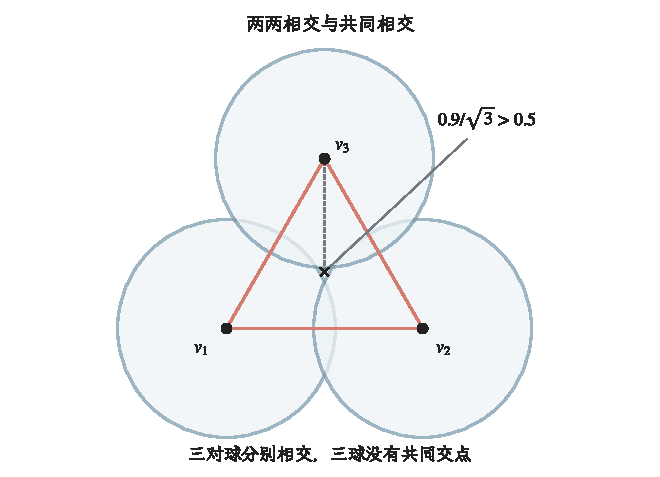
\includegraphics[width=\linewidth]{figures/01-mathematical-preliminaries/02-linear-algebra-and-geometry/matplotlib/teaching-linear-probability/geometry-cech-rips-intersection.pdf}
 \caption{固定同组三点比较共同交集与成对条件。正三角形边长$0.9$，
 $\varepsilon=1$，蓝色开球半径$0.5$；红色边满足两种构造的连边条件。
 三球无共同交点，Čech不含二维面，Rips含二维面。
 中心到各顶点的距离为$0.9/\sqrt3>0.5$。圆周只标开球边界，图为解析教学构造。}
 \label{fig:geometry-cech-rips-intersection}
\end{figure}

尺度变化后仍可给出明确包含关系。对任意$\eta>0$，有
\[
 \mathcal C_\varepsilon\subseteq\mathcal R_\varepsilon
 \subseteq\mathcal C_{2\varepsilon+\eta}.
\]
第一个包含关系由共同交点和三角不等式推出。
对第二个，任选一个顶点作候选共同交点，它到其余顶点的距离至多$\varepsilon$，
严格小于新球半径$\varepsilon+\eta/2$。
若全部球改用闭球，在相应定义下可取尺度常数$2$而不加$\eta$。
这些是足够的普适常数，不声称最紧；同一尺度的复形仍不能互换。

复形何时能代表球并集的拓扑，还依赖覆盖条件。良好覆盖（good cover）要求每个
非空有限交集都可连续收缩到一点；有限欧氏开球的交集为凸集，满足这项要求。
神经引理（nerve lemma）在该条件下说明Čech复形与球并集同伦等价，即二者存在相互映射，
来回复合可以连续变形到恒等映射。这里不要求两映射互为逆，所以比同胚弱：
闭区间可连续收缩到一个点，与单点空间同伦等价，却不可能与它存在双射。
这个结论不等于球并集已经恢复了未知潜在流形；
后者还需要采样覆盖和尺度条件。

为计算未被填充的环，需要把端点抵消与高阶填充分别记录。
选定顶点次序后，以$[v_0,\ldots,v_k]$表示有向单纯形，交换两顶点使符号反转。
有向$k$维单纯形的实系数线性组合称为$k$维链，
组成向量空间$C_k(\mathcal K;\mathbb R)$。边界算子读取每个面的有向边缘：
\begin{equation}
 \partial_k[v_0,\ldots,v_k]
 =\sum_{i=0}^k(-1)^i[v_0,\ldots,\widehat{v_i},\ldots,v_k],
 \qquad k\geq1,
 \label{eq:geometry-simplicial-boundary}
\end{equation}
尖帽表示删去该顶点，算子线性延伸到全部链。
本章采用非约化同调，约定$C_{-1}=\{0\}$、$\partial_0=0$。
例如$\partial_1[1,2]=[2]-[1]$，端点的正负表示方向。

\begin{lemma}[边界的边界为零]
\label{lem:geometry-boundary-squared-zero}
上述算子满足
\begin{equation}
 \partial_{k-1}\partial_k=0,\qquad k\geq1.
 \label{eq:geometry-boundary-squared-zero}
\end{equation}
\end{lemma}
\begin{proof}
$k=1$时由$\partial_0=0$成立。对$k\geq2$，固定$i<j$，
两次删除$v_i,v_j$后得到相同的$(k-2)$维面。
先删$i$再删原来的$j$，系数为$(-1)^i(-1)^{j-1}$；
先删$j$再删$i$，系数为$(-1)^j(-1)^i$，两者相反。
所有项都按这样的顶点对成对抵消，因此结论对基单纯形成立；
由线性性，对全部链成立。
\end{proof}

边界必定闭合，但闭合的圈未必由复形中的某个面填充。
这正好可以用上一章的核、像与商空间表达。
\begin{definition}[闭链、边界与同调空间]
\label{def:geometry-homology-space}
满足$\partial_kc=0$的链称为\term{闭链}（cycle），
能写成$c=\partial_{k+1}b$的链称为\term{边界}（boundary）。
由$\partial_k\partial_{k+1}=0$，有
$\operatorname{im}\partial_{k+1}\subseteq\ker\partial_k$。
实系数\term{同调空间}（homology space）及其维数定义为
\[
 H_k(\mathcal K;\mathbb R)=\ker\partial_k/\operatorname{im}\partial_{k+1},
 \qquad \beta_k=\dim H_k(\mathcal K;\mathbb R).
\]
$\beta_k$称为第$k$个\term{Betti数}（Betti number）。
\end{definition}
商空间沿用定义~\ref{def:linear-algebra-quotient-space}：
两个闭链相差一个边界时被视为同类。因而$H_k$保留的不是全部闭链，
而是无法用已有高阶填充消去的部分；$\beta_0$计算连通分支，
$\beta_1$计算实系数意义下独立的一维环。

取
$\mathcal K_{\mathrm{loop}}
=\{\{1\},\{2\},\{3\},\{1,2\},\{2,3\},\{1,3\}\}$。
链$c=[1,2]+[2,3]-[1,3]$的端点逐一抵消，故$\partial_1c=0$。
$\partial_1$的秩为$2$，一维闭链空间维数为$3-2=1$，
而没有二维面，故$\beta_1=1$、$\beta_0=3-2=1$。
加入$[1,2,3]$后，$c=\partial_2[1,2,3]$成为边界，$\beta_1$降为$0$；
$\partial_1$不变，所以$\beta_0$仍为$1$。
图~\ref{fig:geometry-cycle-filled-simplex}只改变面集合，顶点与边保持相同。
\begin{figure}[htbp]
 \centering
 % Two finite simplicial complexes with the same vertices and edges.
% Intended canvas: 112 mm by 36 mm. Exact combinatorial teaching construction.
\begin{tikzpicture}[x=1cm,y=1cm,font=\figurefont\small,text=FigureInk,
  line width=1.1pt,draw=FigureStroke]
 \path[use as bounding box] (0,0) rectangle (11.2,3.6);
 \begin{scope}[shift={(1.3,0.75)}]
  \coordinate (a) at (0,0); \coordinate (b) at (2.4,0);
  \coordinate (c) at (1.2,1.75);
  \draw (a)--(b)--(c)--cycle;
  \foreach \v in {a,b,c} \fill[FigureInk] (\v) circle (1.3pt);
  \node[below] at (a) {$1$}; \node[below] at (b) {$2$};
  \node[above] at (c) {$3$};
  \node at (1.2,2.5) {空心三角环};
  \node at (1.2,-0.55) {$\beta_1=1$};
 \end{scope}
 \begin{scope}[shift={(7.0,0.75)}]
  \coordinate (a) at (0,0); \coordinate (b) at (2.4,0);
  \coordinate (c) at (1.2,1.75);
  \fill[FigureYellowFill] (a)--(b)--(c)--cycle;
  \draw (a)--(b)--(c)--cycle;
  \foreach \v in {a,b,c} \fill[FigureInk] (\v) circle (1.3pt);
  \node[below] at (a) {$1$}; \node[below] at (b) {$2$};
  \node[above] at (c) {$3$};
  \node at (1.2,2.5) {填充三角面};
  \node at (1.2,-0.55) {$\beta_1=0$};
 \end{scope}
\end{tikzpicture}%

 \caption{一圈边是否已填充，取决于高阶面而非边图。左侧闭链
 $c=[1,2]+[2,3]-[1,3]$不是边界；右侧加入$[1,2,3]$后有
 $c=\partial_2[1,2,3]$。两者$\beta_0=1$，$\beta_1$分别为$1$与$0$。
 图为组合教学示例，不代表某个观测点云的真实拓扑。}
 \label{fig:geometry-cycle-filled-simplex}
\end{figure}

复形的规模还依赖邻域尺度。开带$\mathcal M_{\mathrm{strip}}$与开矩形同胚，
中心线$\mathcal C$与开区间同胚，都没有全局环。
闭合中心线得到圆，保留横向自由度并闭合则得到二维环带；
维数不同，但都保留绕中心的一维环。只有在采样和尺度适当时，样本复形才有理由
反映这些区别。尺度太小会把采样空隙误认作分支；太大则可能跨折连边，
并以高阶面填掉原来的环。

单一尺度可能把采样空隙当成孔洞，也可能把真实孔洞填平。持续同调（persistent homology）
因此跟踪尺度逐渐增大时，同调类何时出现、何时消失。存在于较宽尺度范围内的结构
提供了跨尺度信息，但仍不能仅凭持续时间就认定它对应任务中的真实结构。
若$N_k$是$k$维单纯形数，Euler示性数
$\chi=\sum_k(-1)^kN_k$是更粗的摘要：空心三角形为$3-3=0$，
填充三角形为$3-3+1=1$。由秩--零度关系
$N_k=\beta_k+\operatorname{rank}\partial_k+\operatorname{rank}\partial_{k+1}$，
交替求和后中间秩抵消，也得到$\chi=\sum_k(-1)^k\beta_k$。
不同Betti数组甚至不同拓扑都可能有同一个$\chi$，一个标量不足以代替分别分析。

用硬阈值连边时，两点距离只要稍微超过阈值，就会从相连突然变成不相连。为了记录
接近程度，可以改用软关系，以$\mu_{i,j}\in[0,1]$表示所选局部尺度下的连接强度；
这只是隶属度，不自动是事件概率。高阶强度例如可取全部边强度的最小值，
但必须声明采用哪种规则。一种常见的合并运算是
\begin{equation}
 a\mathbin{\sqcup}b=a+b-ab=1-(1-a)(1-b),\qquad a,b\in[0,1].
 \label{eq:geometry-fuzzy-union}
\end{equation}
结果仍在$[0,1]$内；交换性由对称式给出，结合性由
$1-(1-a)(1-b)(1-c)$给出，$0$为恒等元，任一输入为$1$时输出为$1$。
这些性质使它成为明确定义的软并集，却没有提供独立事件的随机试验或联合分布。
核权重、相似度、置信度与概率的校准要求不能仅凭数值范围混同。

UMAP等方法由局部距离构造带强度的关系，再优化低维坐标以匹配这些关系；
具体目标与优化过程留给
\BookChapterRef{chap:dimensionality-reduction}{第三卷“模型”的“降维”章}。
低维图像中的分离簇或孔洞还可能受邻居数、尺度、初始化与优化误差影响。
拓扑方法不能修复错误的局部输入：跨折捷径会被忠实组合，完全漏采的区域也无法凭空
恢复。采样覆盖、局部关系与尺度共同限制结论。

局部坐标之间的过渡只有在区域衔接时才能复合。若要统一记录这种“有起点和终点的
变换”，可以使用\term{范畴}（category）：
它包含对象、对象之间的箭头及各对象的恒等箭头，
仅在端点匹配时复合箭头，复合满足结合律与恒等律。
函子（functor）把对象和箭头映到另一范畴，同时保持恒等与复合。
例如坐标区域间可复合的过渡可按这种方式记录。
这只是组合表示的延伸语言，本章的距离与同调推导均不依赖它，
也不因引入这些名称获得额外的恢复保证。

\section{非线性空间的局部线性化}
\label{sec:geometry-manifold-local-linearization}

坐标图记录位置，却还没有说明从当前位置可以怎样动。以下固定光滑流形模型，
以局部参数化计算真实的一阶方向，再讨论只有样本时怎样估计这些方向。
解析模型与样本估计解决同一个局部问题，但它们的输入与保证不同。

\subsection{已知参数化下的局部线性化}
\label{sec:geometry-analytic-local-linearization}

从$\bm p=\varphi(\bm z)$出发，坐标变化$\bm v$经Jacobian
$\bm J_\varphi(\bm z)$映为环境空间中的瞬时速度。
\term{切空间}（tangent space）收集所有这样的可行速度；
它描述一阶方向，并不是可行集合本身的一小块。

\begin{definition}[嵌入流形的切空间]
\label{def:geometry-tangent-space}
设$\varphi:U\subseteq\mathbb R^d\to\mathcal M\subseteq\mathbb R^D$
是局部参数化，$\bm p=\varphi(\bm z)$。定义
\begin{equation}
 T_{\bm p}\mathcal M
 =\{\bm J_\varphi(\bm z)\bm v:\bm v\in\mathbb R^d\}.
 \label{eq:geometry-tangent-space-chart}
\end{equation}
\end{definition}
Jacobian列满秩保证这是$d$维向量空间，其原点是零速度。
画在$\bm p$旁边的仿射切平面则是$\bm p+T_{\bm p}\mathcal M$；
点的位置与速度向量的零点不能混为一谈。

\begin{lemma}[曲线速度与坐标刻画相容]
\label{lem:geometry-tangent-curves}
$T_{\bm p}\mathcal M$恰是全部光滑曲线
$\gamma:(-\epsilon,\epsilon)\to\mathcal M$、$\gamma(0)=\bm p$
的速度$\gamma'(0)$组成的集合，并且与局部坐标选择无关。
\end{lemma}
\begin{proof}
在足够小的参数区间内，曲线落入当前坐标图，写成
$\gamma(t)=\varphi(\bm z(t))$。链式法则给出
$\gamma'(0)=\bm J_\varphi(\bm z)\bm z'(0)$，故每个曲线速度都属于所定义的空间。
反过来，任意$\bm v\in\mathbb R^d$给出曲线
$t\mapsto\varphi(\bm z+t\bm v)$；因为$U$开，足够小的$t$仍在定义域内，
其初速度为$\bm J_\varphi(\bm z)\bm v$。

若另一参数化满足$\widetilde\varphi=\varphi\circ\psi$，
坐标过渡$\psi$的Jacobian可逆，且
$\bm J_{\widetilde\varphi}=\bm J_\varphi\bm J_\psi$。
右乘可逆矩阵不改变值域，两张图因而给出同一切空间。
\end{proof}

在点带中直接求导，可核对两个自由度：
\begin{align}
 \frac{\partial\Phi}{\partial s}
 &=\left(1+\frac uR\right)
   \begin{bmatrix}-\sin(s/R)\\\cos(s/R)\end{bmatrix},
 \label{eq:geometry-strip-s-tangent}\\
 \frac{\partial\Phi}{\partial u}
 &=\begin{bmatrix}\cos(s/R)\\\sin(s/R)\end{bmatrix}.
 \label{eq:geometry-strip-u-tangent}
\end{align}
因$|u|<w<R$，第一列不为零，两列正交且线性无关；
开带的切空间是整个$\mathbb R^2$。中心线则只允许$u=0$，
\[
 T_{\Phi(s,0)}\mathcal C
 =\operatorname{span}\{(-\sin(s/R),\cos(s/R))^\top\}.
\]
径向方向对开带可行，对中心线不可行。中心线的切线随位置转动，
没有一条固定线性子空间等于各处的切空间。

图~\ref{fig:geometry-strip-tangent-coordinates}上半部把切向速度画在点旁，
下半部比较同一坐标增量对应的实际弧长。方向数目决定局部维数，
坐标增量怎样换算为长度则留待度量处理。
\begin{figure}[htbp]
 \centering
 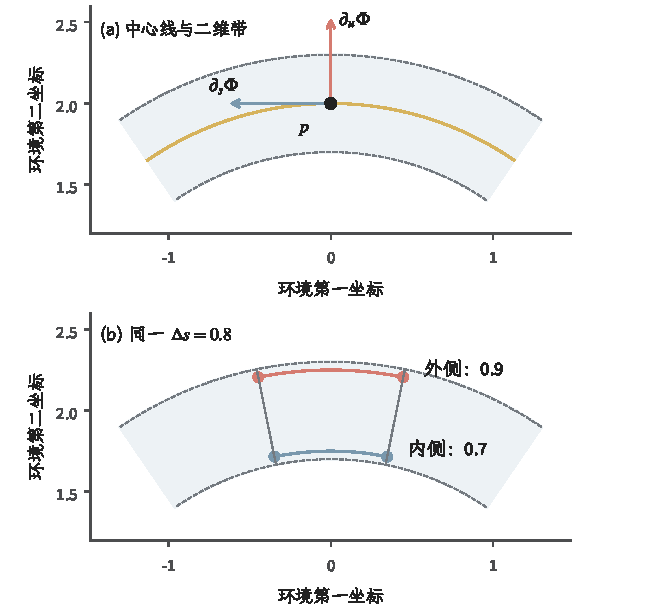
\includegraphics[width=\linewidth]{figures/01-mathematical-preliminaries/02-linear-algebra-and-geometry/matplotlib/concepts-linear-geometry/geometry-strip-tangent-coordinates.pdf}
 \caption{开带与中心线的局部方向不同。取$R=2$、$w=0.3$。
 上图的两个参数方向属于二维开带，仅以中心线为对象时，径向方向不属于其切空间；
 箭头平移到$\bm p$只是画法。下图取$u=-0.25,0.25$，同一$\Delta s=0.8$
 对应圆弧长度$0.7,0.9$。灰虚线为不纳入开带的边界，两图等比例绘制，均为解析教学示例。}
 \label{fig:geometry-strip-tangent-coordinates}
\end{figure}

切空间之所以适合近似，由Taylor展开说明。若参数化在当前邻域内二阶导数有界，则
\begin{equation}
 \varphi(\bm z+\bm h)-\varphi(\bm z)
 =\bm J_\varphi(\bm z)\bm h+O(\lVert\bm h\rVert_2^2).
 \label{eq:geometry-manifold-local-taylor}
\end{equation}
一阶项属于切空间，故环境位移投到法向正交补后只剩二阶余项。
这是局部结论，常数依赖所选邻域及二阶导数界；不能将它延伸到任意大步长。
法向偏离反映嵌入在环境中怎样弯曲，不等于后文要定义的内在曲率。
在二维开带中法向空间为零，弯曲坐标线本身就不构成法向误差。

若流形由约束$F(\bm x)=\bm0$给出，其中
$F:\mathbb R^D\to\mathbb R^{D-d}$在$\bm p$附近光滑且
$\bm J_F(\bm p)$行满秩，就能选出$D-d$列组成可逆方阵。
重排坐标后，定理~\ref{thm:analysis-implicit-function}把这$D-d$个变量
解为其余$d$个变量的光滑函数，后者便给出局部参数化。
对约束内曲线求导得$\bm J_F(\bm p)\gamma'(0)=\bm0$；
所以切空间包含于该矩阵的核。参数化给出$d$维切空间，
秩--零度关系又说明核为$d$维，故$T_{\bm p}\mathcal M=\ker\bm J_F(\bm p)$。
满秩条件不能省略：$F(x,y)=x^2+y^2$在原点导数为零，
核是整个平面，但零水平集只有一个点，真实可行速度只有零向量。

不仅位置可被映射，位置变化也需要随映射传递。
设$F:\mathcal M\to\mathcal N$，其坐标表达
$\psi^{-1}\circ F\circ\varphi$光滑，则称$F$光滑。
它在$\bm p$处的微分（differential）把输入速度转成输出速度：
\[
 \mathrm dF_{\bm p}(\bm v)
 =\left.\frac{\mathrm d}{\mathrm dt}F(\gamma(t))\right|_{t=0},
 \qquad\gamma(0)=\bm p,\quad\gamma'(0)=\bm v.
\]
若$\bm v=\bm J_\varphi(\bm z)\bm a$，令
$\bm w=\psi^{-1}(F(\bm p))$，则
\begin{equation}
 \mathrm dF_{\bm p}(\bm v)
 =\bm J_\psi(\bm w)
   \bm J_{\psi^{-1}\circ F\circ\varphi}(\bm z)\bm a.
 \label{eq:geometry-map-differential}
\end{equation}
右端只依赖初速度，不依赖实现速度的曲线，因此定义良好且线性。
坐标变换时两侧的Jacobian因链式法则相互抵消；
$\mathrm dF_{\bm p}:T_{\bm p}\mathcal M\to T_{F(\bm p)}\mathcal N$
是几何映射，矩阵只是其坐标记录。复合还满足
$\mathrm d(H\circ F)_{\bm p}=\mathrm dH_{F(\bm p)}\circ\mathrm dF_{\bm p}$。

对标量函数$f:\mathcal M\to\mathbb R$，微分读取速度引起的一阶数值变化。
\term{余切空间}（cotangent space）$T_{\bm p}^*\mathcal M$就是
$T_{\bm p}\mathcal M$的线性泛函空间，泛函的含义沿用
定义~\ref{def:functional-bounded-linear-functional}。
有限维向量空间上的全部线性读取组成其对偶空间（dual space）；
所以$\mathrm df_{\bm p}\in T_{\bm p}^*\mathcal M$，不是一个切向量。
写局部坐标为$(z^1,\ldots,z^d)$时，上标在这里是坐标编号而非迭代次数。
坐标切基为$\partial_i=\partial\varphi/\partial z^i$，
其对偶基$\mathrm dz^i$满足$\mathrm dz^i(\partial_j)=\delta_{i,j}$，
也就是$\mathrm dz^i(\sum_j a^j\partial_j)=a^i$：它读出速度的第$i$个坐标系数。于是
\[
 \mathrm df=\sum_i\partial_i(f\circ\varphi)\,\mathrm dz^i,\qquad
 \mathrm df\!\left(\sum_i a^i\partial_i\right)
 =\sum_i\partial_i(f\circ\varphi)a^i.
\]
例如圆上$f(\cos\theta,\sin\theta)=\cos\theta$，
角速度$a$对应的数值变化为$-a\sin\theta$。
要把这个线性读取规则表示成“最陡方向”，还须指定方向长度，
所以梯度将在度量建立后定义。

\subsection{观测样本下的局部线性化}
\label{sec:geometry-sampled-local-linearization}

只有$\bm x_i=\bm p_i+\bm\epsilon_i$时，参数化与潜在位置通常未知。
我们可以考察附近样本主要沿哪些方向变化，用这些方向近似真实切空间。局部PCA
（local principal component analysis）就是按这个思路，在小邻域中寻找主要的线性
变化方向。它估计一个已经选定的流形模型，并不定义流形本身。
必须先说明潜在对象是二维带还是一维中心线，才能确定希望估计什么。

给观测$\bm x_i$选择邻居索引集$N_i$和权重
$\alpha_{i,j}\geq0$、$\sum_{j\in N_i}\alpha_{i,j}=1$，计算
\begin{equation}
 \overline{\bm x}_i=\sum_{j\in N_i}\alpha_{i,j}\bm x_j,\qquad
 \bm C_i=\sum_{j\in N_i}\alpha_{i,j}
  (\bm x_j-\overline{\bm x}_i)(\bm x_j-\overline{\bm x}_i)^\top.
 \label{eq:geometry-local-weighted-covariance}
\end{equation}
若潜在维数$d$给定，取$\bm C_i$最大$d$个特征值对应的正交特征向量
$\widehat{\bm U}_i$，其列空间$\widehat T_i$为估计方向子空间。
若$d$未知，需另由谱和误差模型判断；不能把预先指定的特征向量数当成维数发现。
局部均值消去样本位置偏移，但不保证等于$\bm p_i$。

计算结果要与真实对象分开。$T_{\bm p_i}\mathcal M$是潜在位置处的真实方向空间，
$\widehat T_i$是从样本估计出的方向空间，二者都以零速度为原点。把估计方向空间
平移到$\overline{\bm x}_i$或$\bm x_i$处，才得到图中画出的仿射切平面近似。
若$d<D$，一般环境噪声使$\bm x_i\notin\mathcal M$，
此时$T_{\bm x_i}\mathcal M$甚至没有定义。
二维开带是当前例外：小噪声下观测仍在开带内，其切空间仍为$\mathbb R^2$，
但这不表示已经识别出生成它的潜在位置。

式~\eqref{eq:geometry-manifold-local-taylor}解释了误差来源。
在正则局部坐标中，邻域尺度为$h$时，切向位移通常为$O(h)$，
嵌入法向偏离为$O(h^2)$。若采样在各切方向上充分展开，
切向协方差特征值具有$h^2$量级；法向位移的平方贡献则可达到$h^4$量级。
这些尺度比较需要二阶导数有界和非退化局部采样，单靠光滑性并不保证谱间隙。

上一章的子空间扰动结论可用于把误差变成方向误差：
若理想局部协方差在第$d$与第$d+1$特征值间有间隙$\delta>0$，
而观测造成的算子范数扰动相对$\delta$足够小，则估计子空间的偏转受
$\lVert\bm E\rVert_2/\delta$控制。这里$\bm E$要包括有限样本波动、
噪声、邻域错选及非线性近似误差，不能只代入测量噪声方差。

缩小邻域会降低法向二阶偏差，却减少样本并压低真实信号的谱尺度；
固定噪声不会随之自动消失。邻域过大时，中心线不同位置的切线已经明显转动，
PCA会把这些不同方向合在一起，结果未必接近中心点的切线。对二维窄带，若样本的横向覆盖不足或宽度小于噪声尺度，
第二个方向可能难以稳定识别，但潜在对象并不因此变成一维。
固定近邻数也不能解决非均匀密度带来的变化：稀疏处覆盖范围大，稠密处范围小。
潜在对象、采样密度、嵌入弯曲、邻域尺度、谱间隙和噪声必须一起解释。

即使局部方向估计准确，也尚未得到全局坐标。圆的每个邻域只有一个切方向，
却不能以单张无断点实坐标图覆盖。局部PCA提供的是后续几何计算的局部输入，
不是全局展开或任务语义正确性的保证。

\section{流形上相同切空间下的度量、距离与运动}
\label{sec:geometry-metric-path-geodesic}

这里每次比较的两个向量，都属于同一个点处的切空间。
沿路径时，速度可以属于随位置变化的切空间；计算长度只需在每个位置读出一个标量速度，
再把这些标量累计起来，不需要先把不同位置的向量搬到一起。

\subsection{同一点处的切向量度量}
\label{sec:geometry-same-point-metric}

切空间说明方向可不可行，却没有规定一单位坐标变化有多长。
点带外侧与内侧相同的$\mathrm ds$对应不同弧长，因而内积必须按位置指定。
\term{Riemann度量}（Riemannian metric）为每个切空间提供这种长度与夹角规则。

\begin{definition}[Riemann度量]
\label{def:geometry-riemannian-metric}
光滑流形$\mathcal M$上的Riemann度量$g$为每个$\bm p$指定内积
$g_{\bm p}:T_{\bm p}\mathcal M\times T_{\bm p}\mathcal M\to\mathbb R$，
且在任一光滑坐标切基$\partial_i$中，矩阵
$\bm G(\bm z)=[g_{i,j}(\bm z)]$、$g_{i,j}=g(\partial_i,\partial_j)$
的条目光滑。每个$\bm G$都对称正定。
\end{definition}
对同点切向量$\bm v,\bm w$，长度为
$\lVert\bm v\rVert_g=\sqrt{g_{\bm p}(\bm v,\bm v)}$；
非零时夹角满足
$\cos\vartheta=g_{\bm p}(\bm v,\bm w)/
(\lVert\bm v\rVert_g\lVert\bm w\rVert_g)$。
若它们的坐标分量为$\bm a,\bm b$，内积是$\bm a^\top\bm G\bm b$。
$\bm G$既不是样本协方差，也不必是全空间共享的常矩阵。

嵌入流形可以限制环境欧氏内积，得到诱导度量：
\begin{equation}
 \bm G(\bm z)=\bm J_\varphi(\bm z)^\top\bm J_\varphi(\bm z).
 \label{eq:geometry-induced-metric}
\end{equation}
对非零$\bm a$，满列秩保证
$\bm a^\top\bm G\bm a=\lVert\bm J_\varphi\bm a\rVert_2^2>0$。
若Jacobian退化，只会得到半正定形式；这不符合当前坐标中的Riemann度量条件。
也可以另选光滑正定内积，但这样会改变几何，而不只是改写坐标。

若旧坐标$\bm z=\psi(\bm v)$，记可逆Jacobian为$\bm A=\bm J_\psi$，
同一几何向量的旧分量等于$\bm A$乘新分量，所以
\begin{equation}
 \widetilde{\bm G}(\bm v)=
 \bm A^\top\bm G(\psi(\bm v))\bm A.
 \label{eq:geometry-metric-coordinate-transform}
\end{equation}
因此$\bm a^\top\widetilde{\bm G}\bm b
=(\bm A\bm a)^\top\bm G(\bm A\bm b)$。
改变分量而不改变度量会改变所计算的长度；按此式一起变换则仍描述同一内积。

点带的两个参数方向已在式~\eqref{eq:geometry-strip-s-tangent}与
\eqref{eq:geometry-strip-u-tangent}中求出，故
\begin{equation}
 \bm G(s,u)=
 \begin{bmatrix}(1+u/R)^2&0\\0&1\end{bmatrix}.
 \label{eq:geometry-strip-metric}
\end{equation}
横向速度$\dot u$的长度系数为$1$，纵向速度$\dot s$的系数为$1+u/R$。
在$R=2$、$u=\pm0.25$时，同一$\Delta s=0.8$沿固定$u$的圆弧
分别产生$0.9$与$0.7$的长度，与图~\ref{fig:geometry-strip-tangent-coordinates}一致。
内积权重来自坐标尺度，并不由该位置采到了多少点决定。

\subsection{沿路径的速度与长度}
\label{sec:geometry-path-speed-length}

设分段光滑路径$\gamma:[a,b]\to\mathcal M$在一张图中写成
$\gamma(t)=\varphi(\bm z(t))$。链式法则保证
$\dot\gamma(t)\in T_{\gamma(t)}\mathcal M$，度量读出的平方速度为
\begin{equation}
 \lVert\dot\gamma(t)\rVert_g^2
 =\dot{\bm z}(t)^\top\bm G(\bm z(t))\dot{\bm z}(t).
 \label{eq:geometry-riemannian-speed}
\end{equation}
将标量速度按时间累计，定义路径长度
\begin{equation}
 L_g(\gamma)=\int_a^b
 \sqrt{\dot{\bm z}(t)^\top\bm G(\bm z(t))\dot{\bm z}(t)}\,\mathrm dt.
 \label{eq:geometry-riemannian-curve-length}
\end{equation}
整条路径不在同一张图时，将紧区间$[a,b]$分成有限段，使每段落入一张图，
再求长度之和。紧致的路径像和坐标开覆盖保证能作这种有限分段。

这种计算不依赖坐标。在$\bm z=\psi(\bm v)$下，
$\dot{\bm z}=\bm A\dot{\bm v}$，
式~\eqref{eq:geometry-metric-coordinate-transform}给出
$\dot{\bm v}^\top\widetilde{\bm G}\dot{\bm v}
=\dot{\bm z}^\top\bm G\dot{\bm z}$。
每段被积的标量相同，所以重叠区域选哪张图、怎样进一步细分都不改变长度。

长度也不依赖沿同一路线前进的快慢。对保持方向的光滑重参数化$t=\tau(r)$，
新速度为$\dot\gamma(\tau(r))\tau'(r)$，
其长度因子为$|\tau'(r)|$；当$\tau'>0$时，
积分换元$\mathrm dt=\tau'(r)\mathrm dr$给出相同总长。
反向的光滑单调参数化配合积分端点互换也不改变长度。
允许停顿的分段正则重参数化可分段处理；来回多走则改变路线的经过次数，
不属于仅仅换速度。

瞬时切向可行不等于环境直线可行。单位圆上
$\bm p=(1,0)^\top$、$\bm v=(0,1)^\top\in T_{\bm p}\mathbb S^1$，
但$\lVert\bm p+t\bm v\rVert_2=\sqrt{1+t^2}>1$对$t\neq0$成立。
速度只描述路径的一阶变化，保持有限步可行仍需在曲面上构造完整路径或更新映射。

\subsection{固定端点间的测地距离与近似}
\label{sec:geometry-endpoint-distance}

路径长度评价一条已经给出的路线。端点固定而路线可选时，要比较所有允许的路线；
完整空间已知和只有有限采样是这个问题的两种信息条件。

\subsubsection{连续空间下的测地距离}
\label{sec:geometry-continuous-geodesic-distance}

\begin{definition}[测地距离]
\label{def:geometry-geodesic-distance}
在Riemann流形$(\mathcal M,g)$的同一路径连通分支内，定义
\term{测地距离}（geodesic distance）为连接两点的全部分段光滑路径长度的下确界：
\begin{equation}
 d_g(\bm p,\bm q)=
 \inf_{\substack{\gamma(a)=\bm p\\\gamma(b)=\bm q}}L_g(\gamma).
 \label{eq:geometry-geodesic-distance}
\end{equation}
若无连接路径，约定值为$+\infty$；在可能不连通的整个空间上，它是扩展距离。
\end{definition}
这里的定义尚不要求存在最短路径，更不依赖测地线方程。
反向路径给出对称性，拼接两条近似最短路径给出三角不等式。
在一个足够小的坐标邻域内，按度量计算的向量长度，可以用其坐标向量的欧氏长度
乘以两个固定正常数从上下控制。这保证不同点之间的路程不能趋于零，因而每个
连通分支中确实得到度量。

对于欧氏诱导度量，由
$\bm q-\bm p=\int_a^b\dot\gamma(t)\,\mathrm dt$与三角不等式，
每条连接路径均满足$\lVert\bm q-\bm p\rVert_2\leq L_g(\gamma)$，
所以
\[
 \lVert\bm q-\bm p\rVert_2\leq d_g(\bm p,\bm q).
\]
若连接线段完全可行，就取等。反过来，只有下确界被允许路径达到时，
取等才迫使该最短路径沿线段行进，至多改变速度；
距离相等本身不保证线段可行。若换成任意非诱导度量，上述环境距离比较也不能照搬。

回到开中心线的两点$\bm p=\Phi(s,0)$、$\bm q=\Phi(t,0)$。
环境空间的弦长是
\begin{equation}
 \lVert\Phi(s,0)-\Phi(t,0)\rVert_2
 =2R\left|\sin\frac{s-t}{2R}\right|.
 \label{eq:geometry-strip-chord-distance}
\end{equation}
中心线以$s$为弧长参数，允许路径必须留在开弧内，因此
$d_{\mathcal C}(\bm p,\bm q)=|s-t|$。
二维带允许路径向内侧绕行，中心线弧只是候选，故
\[
 \lVert\bm p-\bm q\rVert_2
 \leq d_{\mathcal M_{\mathrm{strip}}}(\bm p,\bm q)
 \leq d_{\mathcal C}(\bm p,\bm q)=|s-t|.
\]
带宽、端点位置和允许域决定第二个不等式是否严格；
不能把这两种距离都称为不加区分的“沿带距离”。

另取完整单位圆作为独立例子。夹角$0\leq\theta\leq\pi$时，
允许选择短弧，内在距离为$\theta$，弦长为$2\sin(\theta/2)$。
在$\theta=\pi/2$时两者为$\pi/2$与$\sqrt2$；
小角度展开$2\sin(\theta/2)=\theta-\theta^3/24+O(\theta^5)$说明局部接近，
全局却不同。图~\ref{fig:geometry-circle-distances}在相同尺度上比较这两种量。
\begin{figure*}[htbp]
 \centering
 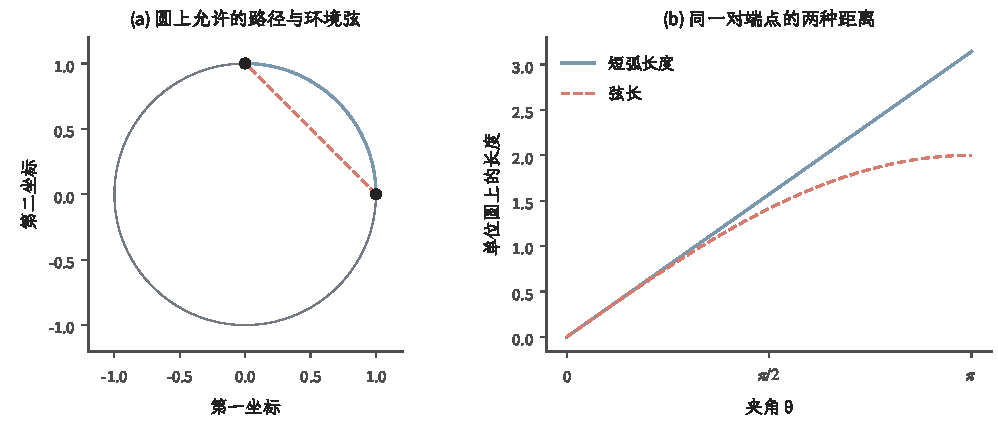
\includegraphics[width=\linewidth]{figures/01-mathematical-preliminaries/02-linear-algebra-and-geometry/matplotlib/analysis-geometry/geometry-circle-distances.pdf}
 \caption{完整单位圆的测地距离与环境弦长。左图夹角为$\pi/2$，
 蓝线为圆上的允许短弧，红虚线为穿过圆内的环境线段；
 右图比较$\theta\in[0,\pi]$时的两种长度。完整圆允许选择两段弧中的较短者，
 不能与开中心线或二维开带的允许路径混用。图为解析教学示例。}
 \label{fig:geometry-circle-distances}
\end{figure*}

为什么定义取下确界，而不直接取最小值？因为允许的路径未必包含一条最短路径。在穿孔平面
$\mathbb R^2\setminus\{\bm0\}$中，$(-1,0)^\top$与$(1,0)^\top$
之间可绕过任意小的圆孔，路径长度趋于$2$，却没有长度恰为$2$的允许路径。
哪些全局条件保证达到下确界，将在固定端点的最短路径问题中讨论。

\subsubsection{有限采样下的测地距离近似}
\label{sec:geometry-sampled-geodesic-distance}

只有观测点时，常把距离小于阈值$\varepsilon$的点相连，
或连接每个点的$k$个最近邻，再以$\lVert\bm x_i-\bm x_j\rVert_2$为边长。
一条边路径的长度是所经边长之和，最短边路径试图近似所选潜在流形上
$d_g(\bm p_i,\bm p_j)$。这里只借用顶点、边和路径的直观含义，
通用图算法留给第~\ref{part:discrete-mathematics-and-graph-theory}部分。

潜在对象必须先定。若观测不在潜在流形上，$d_g(\bm x_i,\bm x_j)$便未定义；
即使观测在二维开带内，也不能因此把它认作$\bm p_i$。
环境欧氏边长自然对应欧氏诱导度量的局部近似；
若目标采用另一个Riemann度量，就要据此修正边长，不能继续沿用欧氏弦长而声称目标未变。

邻域应足够小，使每条边只连接潜在流形上近似平直的一小段，避免把环境中靠得很近、
沿流形却相距很远的两段直接相连；
又要大到样本间的空隙能够连通。超过跨折环境间隔会引入捷径，低估沿潜在空间的距离；
小于采样空隙则会把一个真实分支拆开，返回无穷距离。
即使没有捷径，局部弦长误差与离散路径绕行误差也会共同作用，
不能无条件断言估计总在真实距离的同一侧。

固定$k$并不固定几何尺度。稀疏处第$k$个邻居可能很远，稠密处则很近，
有向近邻关系还可能不对称，需要声明如何对称化。
一致近似通常要求潜在流形光滑、采样在所研究区域逐渐稠密、
噪声相对邻域尺度受控，并让邻域半径随样本量缩小而仍足以覆盖采样空隙。
非紧开带若只在一部分采样，这些要求也只支持相应覆盖区域的结论。
具体收敛速度须结合采样分布与尺度选择证明，
最短边路径正确更不自动意味着后续全局坐标恢复正确。

\subsection{度量诱导的体积与积分}
\label{sec:geometry-riemannian-volume}

沿路径积分只覆盖一条路线。若要在整个曲面上累计函数值或变化量，就需要知道
每个小区域占多大面积；更高维时，相应的量是体积。
坐标切基围成的微小平行体，其平方体积是Gram行列式$\det\bm G$，
因此几何体积元为
\begin{equation}
 \mathrm dV_g=\sqrt{\det\bm G(\bm z)}\,\mathrm d\bm z.
 \label{eq:geometry-riemannian-volume}
\end{equation}
这是由度量产生的测度密度，不要求先为流形选定全局朝向。
一维时给出长度，二维时给出面积。

坐标变换$\bm z=\psi(\bm v)$下，
$\det\widetilde{\bm G}=(\det\bm A)^2\det\bm G$，所以
\[
 \sqrt{\det\widetilde{\bm G}}\,\mathrm d\bm v
 =\sqrt{\det\bm G(\psi(\bm v))}\,|\det\bm A|\,\mathrm d\bm v.
\]
它正是多元积分换元中的Jacobian因子，故对可积函数所得积分不依赖坐标。
跨图时必须避免把重叠区域重复计数，可分割成可测片段分别积分；
光滑计算也可使用从属于图册、和为$1$的局部权重来拼接。

点带中$\sqrt{\det\bm G}=1+u/R>0$，
小盒$\mathrm ds\,\mathrm du$在外侧对应较大面积。
中心线限制为$u=0$后的一维体积元是$\mathrm ds$，不是把二维面积直接代入。
若样本相对几何体积有密度$q$，其分布测度是$q\,\mathrm dV_g$；
简单样本平均近似该加权积分，并非自动近似$\int f\,\mathrm dV_g$。
几何体积与采样权重的差别将在离散平滑目标中再次出现。

当前开带无流形边界，但不是紧集。需要边界积分时，将另取有分片光滑边界的
截断闭域，并声明函数在边界的行为；不能只因图上画有虚线就把它当作同一个积分问题。

\section{流形上不同切空间的比较与曲率}
\label{sec:geometry-cross-point-comparison-curvature}

沿路径计算长度时，每个位置只输出一个标量。若要问速度有没有转弯，
或相邻两点的方向是否一致，就必须比较不同切空间中的向量。
即使流形嵌在同一个欧氏空间内，直接相减也可能产生法向分量：
圆上恒速运动的速度导数指向圆心，却没有沿圆加速。
需要把环境变化与流形内的方向变化分开。下面建立联络、测地运动和曲率，
所用的Riemann几何基础可参见Lee的教材\scite{math-lee2018riemannian}

\subsection{不同切空间的比较规则}
\label{sec:geometry-connection-comparison}

在每个位置指定一个可行方向，得到向量场。跨点比较规则应使其导数仍为切向量，
还应遵守加法和乘积求导；联络就是满足这些要求的微分规则。
它不是把所有切空间强行认成同一个空间，而是在局部说明怎样比较变化。

\begin{definition}[向量场与联络]
\label{def:geometry-connection}
光滑\term{向量场}（vector field）$\bm V$在每个$\bm p\in\mathcal M$选取
$\bm V(\bm p)\in T_{\bm p}\mathcal M$，其坐标分量光滑。
\term{联络}（connection）为两个光滑向量场$\bm U,\bm V$指定向量场
$\nabla_{\bm U}\bm V$，称为$\bm V$沿$\bm U$的
\term{协变导数}（covariant derivative），并满足
\[
 \begin{aligned}
 \nabla_{f\bm U+h\bm W}\bm V
   &=f\nabla_{\bm U}\bm V+h\nabla_{\bm W}\bm V,\\
 \nabla_{\bm U}(a\bm V+b\bm W)
   &=a\nabla_{\bm U}\bm V+b\nabla_{\bm U}\bm W,\\
 \nabla_{\bm U}(f\bm V)
   &=\bm U(f)\bm V+f\nabla_{\bm U}\bm V.
 \end{aligned}
\]
其中$f,h$为光滑函数，$a,b\in\mathbb R$，
$\bm U(f)=\mathrm df(\bm U)$为方向导数。
\end{definition}
第一条允许求导方向的系数是光滑函数，第二条只允许被求导向量场的系数是常数，
第三条说明为什么不能把第二条的常数任意换成光滑函数：
系数本身的变化必须保留。欧氏空间的普通方向导数满足这三项规则；
一般流形上，单独求坐标分量的导数不够，因为坐标切基本身也在变。

度量已经规定长度，新的导数应当与这一判断相容。
此外，非坐标方向场先后作用的顺序本来就可能不同，不能把这种差异误认为额外的几何扭转。
定义交换子$[\bm U,\bm V]$为对任意光滑$f$满足
\[
 [\bm U,\bm V](f)=\bm U(\bm V(f))-\bm V(\bm U(f))
\]
的向量场；在坐标基下，其第$k$个分量为
$\sum_i(U^i\partial_iV^k-V^i\partial_iU^k)$。
坐标方向$\partial_i,\partial_j$的交换子为零，一般方向场则未必。

\begin{example}[平面上不可交换的方向场]
\label{ex:geometry-plane-field-commutator}
在欧氏平面取$\bm U=\partial_x$、$\bm V=x\partial_y$。
$\bm U$始终沿$x$轴，$\bm V$沿$y$轴但其大小随$x$改变。
对任意光滑函数$f$，
\[
 \bm U(\bm V(f))=\partial_yf+x\partial_x\partial_yf,\qquad
 \bm V(\bm U(f))=x\partial_y\partial_xf,
\]
故$[\bm U,\bm V]=\partial_y$。先沿$x$方向移动，会改变随后沿$\bm V$移动的速度；
两个方向场的顺序差异在平面上就会出现。
欧氏空间的普通方向导数还给出
\[
 \nabla_{\bm U}\bm V=\partial_y,\qquad
 \nabla_{\bm V}\bm U=\bm0.
\]
二者之差恰是交换子。这个平坦例子说明，方向场本身随位置变化所产生的差异，
需要与几何结构额外产生的差异分开。
\end{example}

\begin{definition}[Levi--Civita联络]
\label{def:geometry-levi-civita-connection}
给定Riemann度量$g$，同时满足下列度量相容与无挠条件的联络，
称为它的\term{Levi--Civita联络}（Levi--Civita connection）：
\begin{align*}
 \bm U\bigl(g(\bm V,\bm W)\bigr)
 &=g(\nabla_{\bm U}\bm V,\bm W)+g(\bm V,\nabla_{\bm U}\bm W),\\
 \nabla_{\bm U}\bm V-\nabla_{\bm V}\bm U&=[\bm U,\bm V].
\end{align*}
\end{definition}
度量相容使内积的求导仍满足乘积法则；无挠规定联络在交换两个方向场时，
不产生交换子之外的差异。无挠\emph{不}声称
$\nabla_{\bm U}\nabla_{\bm V}\bm W
=\nabla_{\bm V}\nabla_{\bm U}\bm W$，后者涉及本节末尾的曲率。

每个光滑Riemann度量唯一确定这样的联络。其唯一性可以从两项条件直接看出：
轮换$\bm U,\bm V,\bm W$的度量相容等式，并用无挠条件消去交换项，得到
\begin{align}
 2g(\nabla_{\bm U}\bm V,\bm W)
 &=\bm U g(\bm V,\bm W)+\bm V g(\bm W,\bm U)
   -\bm W g(\bm U,\bm V)\notag\\
 &\quad+g([\bm U,\bm V],\bm W)-g([\bm V,\bm W],\bm U)
   +g([\bm W,\bm U],\bm V).
 \label{eq:geometry-koszul-formula}
\end{align}
右端只含已知度量、向量场和普通方向导数；正定性使其唯一确定
$\nabla_{\bm U}\bm V$。反过来，用此式定义该向量场，代入可检查联络的三条规则、
度量相容和无挠条件，因而也给出存在性。这个公式的用途是确定比较规则，
实际计算通常使用坐标系数或环境投影。

对继承欧氏度量的嵌入流形，设$\bm P_{\bm p}$为环境空间到
$T_{\bm p}\mathcal M$的正交投影，则
\begin{equation}
 \nabla_{\bm U}\bm V(\bm p)
 =\bm P_{\bm p}\,\mathrm d\bm V_{\bm p}(\bm U(\bm p)).
 \label{eq:geometry-projected-connection}
\end{equation}
这里把$\bm V$视为取值于环境$\mathbb R^D$的映射，先求环境导数再投影。
投影保持对切向量的内积，所以欧氏内积的乘积法则给出度量相容；
环境方向导数之差是已经切向的交换子，投影后仍不变，故也无挠。
由唯一性，这正是诱导度量的Levi--Civita联络。
若度量不是环境诱导度量，不能继续沿用这个欧氏正交投影公式。

\subsection{给定路径下的平行移动}
\label{sec:geometry-parallel-transport}

现在固定路径$\gamma(t)$和起点切向量，希望沿路保持方向。
“保持”不是要求环境坐标分量不变，而是要求联络测得的变化为零。
在坐标基中写
$\nabla_{\partial_i}\partial_j=\sum_k\Gamma^k_{i,j}\partial_k$，
则沿$\gamma(t)=\varphi(\bm z(t))$的向量
$\bm V(t)=\sum_jV^j(t)\partial_j$满足
\begin{equation}
 \frac{D\bm V}{\mathrm dt}
 =\sum_k\left(\dot V^k+
     \sum_{i,j}\Gamma^k_{i,j}(\bm z(t))\dot z^iV^j\right)\partial_k.
 \label{eq:geometry-covariant-derivative-along-path}
\end{equation}
第一项是分量变化，第二项修正坐标切基的变化；合起来才是坐标无关的协变导数。
对于欧氏诱导度量，式~\eqref{eq:geometry-projected-connection}沿路径写成
\[
 \frac{D\bm V}{\mathrm dt}
 =\bm P_{\gamma(t)}\frac{\mathrm d\bm V}{\mathrm dt},
\]
保留环境导数的切向部分。

\begin{definition}[平行移动]
\label{def:geometry-parallel-transport}
给定分段光滑路径$\gamma:[a,b]\to\mathcal M$和
$\bm v\in T_{\gamma(a)}\mathcal M$，沿路解
\[
 \frac{D\bm V}{\mathrm dt}=\bm0,\qquad \bm V(a)=\bm v.
\]
终值定义线性映射
$P_\gamma:T_{\gamma(a)}\mathcal M\to T_{\gamma(b)}\mathcal M$，
称为沿$\gamma$的\term{平行移动}（parallel transport）。
\end{definition}
坐标式是具有连续系数的线性常微分方程，初值唯一决定解；
沿有限段路径逐图求解并拼接即可，不要求流形完备。
反向路径给出逆映射，拼接路径对应映射复合。
对于Levi--Civita联络，
\[
 \frac{\mathrm d}{\mathrm dt}g(\bm V,\bm W)
 =g(D\bm V/\mathrm dt,\bm W)+g(\bm V,D\bm W/\mathrm dt)=0
\]
用于任意两个平行向量场。因此$P_\gamma$保持长度和夹角。
这个结论依赖度量相容，不能对任意联络直接宣称保距。

欧氏空间的直角坐标中$\Gamma^k_{i,j}=0$，平行移动保持向量的分量不变，
且与路径无关。球面则不同：向量必须始终切向，环境分量通常会改变，
不同路径的终值也可能不同。

\begin{example}[球面三段路径上的方向搬运]
\label{ex:geometry-sphere-parallel-transport}
在诱导度量的单位球面$\mathbb S^2$上，取
$N=(0,0,1)^\top$、$A=(1,0,0)^\top$、$B=(0,1,0)^\top$。
记三个坐标轴的单位向量为$\bm e_x,\bm e_y,\bm e_z$。
沿三条四分之一大圆弧$N\to A\to B\to N$搬运初始向量
$\bm V(N)=\bm e_x$。各段用$t\in[0,\pi/2]$参数化：
\[
 \begin{array}{c|c|c}
  \text{路径}&\gamma(t)&\bm V(t)\\ \hline
  N\to A&(\sin t,0,\cos t)^\top&(\cos t,0,-\sin t)^\top\\
  A\to B&(\cos t,\sin t,0)^\top&(0,0,-1)^\top\\
  B\to N&(0,\cos t,\sin t)^\top&(0,\sin t,-\cos t)^\top
 \end{array}
\]
每段都有$\gamma^\top\bm V=0$与$\lVert\bm V\rVert_2=1$。
第一段$\dot{\bm V}=-\gamma$，第二段$\dot{\bm V}=\bm0$，
第三段$\dot{\bm V}=\gamma$，环境导数全部是法向或零，投影后的协变导数为零。
两处接点的向量同为$-\bm e_z$，故三段连续拼接。
返回$N$时向量成为$\bm e_y$，与初始$\bm e_x$相差$\pi/2$。
若始终留在$N$，搬运则不改变向量，说明仅给起终点不能决定平行移动。
\end{example}

图~\ref{fig:geometry-sphere-parallel-transport}画出这些向量的沿路变化。
在$B\to N$段，向量与前进速度相反；保持方向不意味着向量必须指向前进方向。
\begin{figure}[htbp]
 \centering
 % Orthographic projection: x=(y-x)/sqrt(2), y=(2z-x-y)/sqrt(6).
% All tangent arrows have the same length before projection.
\begin{tikzpicture}[figure picture,x=1mm,y=1mm,
  transport/.style={draw=FigureRed,line width=.95pt,
    -{Stealth[length=1.8mm,width=1.2mm]}},
  route/.style={draw=FigureBlue,line width=1.1pt,
    -{Stealth[length=1.8mm,width=1.2mm]}},
  every node/.append style={fill=none,inner sep=1.2pt}]
 \path[use as bounding box] (0,10) rectangle (112,77);
 \begin{scope}[shift={(56,40)}]
  \draw[FigureGrid] (0,0) circle[radius=28];
  \draw[FigureGrid,dashed,samples=81,domain=135:315]
   plot ({28/sqrt(2)*(sin(\x)-cos(\x))},
         {-28/sqrt(6)*(cos(\x)+sin(\x))});
  \draw[FigureGrid,samples=81,domain=-45:135]
   plot ({28/sqrt(2)*(sin(\x)-cos(\x))},
         {-28/sqrt(6)*(cos(\x)+sin(\x))});
  \draw[route,samples=61,domain=0:90]
   plot ({-28/sqrt(2)*sin(\x)},
         {28/sqrt(6)*(2*cos(\x)-sin(\x))});
  \draw[route,samples=61,domain=0:90]
   plot ({28/sqrt(2)*(sin(\x)-cos(\x))},
         {-28/sqrt(6)*(cos(\x)+sin(\x))});
  \draw[route,samples=61,domain=0:90]
   plot ({28/sqrt(2)*cos(\x)},
         {28/sqrt(6)*(2*sin(\x)-cos(\x))});
  \foreach \t in {30,60} {
   \draw[transport]
    ({-28/sqrt(2)*sin(\t)},{28/sqrt(6)*(2*cos(\t)-sin(\t))})
    -- ++({-11/sqrt(2)*cos(\t)},
          {11/sqrt(6)*(-2*sin(\t)-cos(\t))});
   \draw[transport]
    ({28/sqrt(2)*(sin(\t)-cos(\t))},
     {-28/sqrt(6)*(cos(\t)+sin(\t))})
    -- ++(0,{-22/sqrt(6)});
   \draw[transport]
    ({28/sqrt(2)*cos(\t)},{28/sqrt(6)*(2*sin(\t)-cos(\t))})
    -- ++({11/sqrt(2)*sin(\t)},
          {11/sqrt(6)*(-2*cos(\t)-sin(\t))});
  }
  \coordinate (N) at (0,{56/sqrt(6)});
  \coordinate (A) at ({-28/sqrt(2)},{-28/sqrt(6)});
  \coordinate (B) at ({28/sqrt(2)},{-28/sqrt(6)});
  \draw[draw=FigureYellow,line width=1.2pt,
    -{Stealth[length=2mm,width=1.4mm]}]
    (N)--++({-11/sqrt(2)},{-11/sqrt(6)}) coordinate (Initial);
  \draw[transport] (N)--++({11/sqrt(2)},{-11/sqrt(6)})
    coordinate (Final);
  \foreach \p in {N,A,B} {\fill[FigureInk] (\p) circle[radius=.6];}
  \node[above] at (N) {$N$};
  \node[below left] at (A) {$A$};
  \node[below right] at (B) {$B$};
 \end{scope}
 \draw[FigureMuted,line width=.4pt] (Initial)--(36,70)--(26,70);
 \node[above] at (26,70) {初始 $\bm e_x$};
 \draw[FigureMuted,line width=.4pt] (Final)--(76,70)--(87,70);
 \node[above] at (87,70) {终值 $\bm e_y$};
\end{tikzpicture}

 \caption{单位球面上沿$N\to A\to B\to N$的平行移动。
 蓝色为给定的三条大圆弧，红箭头为例~\ref{ex:geometry-sphere-parallel-transport}
 中逐段计算的切向量。沿路协变导数为零，返回$N$后的方向却由黄色初始箭头
 $\bm e_x$变为红色终值箭头$\bm e_y$。
 箭头在三维中等长，投影到纸面后的长度可以不同。图为解析教学示例。}
 \label{fig:geometry-sphere-parallel-transport}
\end{figure}

这里的变换由路径和联络决定，不是任意选一个旋转来对齐环境向量。
前文群作用规定的是输入在指定变换下的响应；平行移动规定的是沿几何路径的方向比较，
即使二者有时都用矩阵表示，也不能据此互换。

\subsection{不同条件下的测地运动与最短路径}
\label{sec:geometry-geodesic-motion-minimization}

平行移动把路径当作输入、向量场当作未知量。若要求路径自己的速度平行移动，
路径也变成未知量。给定初速度时，这是运动方程的初值问题；
只给两个端点时，还要决定该沿哪条路径前进，最短性是额外的比较要求。

\subsubsection{初速度条件下的测地运动}
\label{sec:geometry-geodesic-initial-value}

\begin{definition}[测地线]
\label{def:geometry-geodesic}
相对于Riemann流形的Levi--Civita联络，采用仿射参数的曲线$\gamma$若满足
\[
 \frac{D\dot\gamma}{\mathrm dt}=\bm0,
\]
称为\term{测地线}（geodesic）。
\end{definition}
它没有切向加速度，速度沿自身路径作平行移动。
度量相容进一步给出
$\frac{\mathrm d}{\mathrm dt}\lVert\dot\gamma\rVert_g^2
=2g(D\dot\gamma/\mathrm dt,\dot\gamma)=0$，因此速度大小恒定。
环境加速度仍可非零，例如球面大圆需要法向加速度才能留在球面。

“仿射参数”说明换元$t=ar+b$、$a\neq0$保留这个方程。
一般换元则产生
\[
 \frac{D}{\mathrm dr}\frac{\mathrm d\gamma}{\mathrm dr}
 =(\tau'(r))^2\frac{D\dot\gamma}{\mathrm dt}
   +\tau''(r)\dot\gamma.
\]
非匀速参数化可以描出相同几何轨迹，却不再满足零协变加速度。
因此不能把路径长度的任意重参数化不变性照搬到这个运动方程。

要在坐标中求解，先用式~\eqref{eq:geometry-koszul-formula}取
$\bm U=\partial_i,\bm V=\partial_j,\bm W=\partial_\ell$。
坐标方向交换子为零，于是
\[
 2\sum_k g_{k,\ell}\Gamma^k_{i,j}
 =\partial_i g_{j,\ell}+\partial_j g_{i,\ell}-\partial_\ell g_{i,j}.
\]
乘逆度量便得到Christoffel符号
\begin{equation}
 \Gamma^k_{i,j}
 =\frac12\sum_{\ell=1}^d g^{k,\ell}
  \left(\frac{\partial g_{\ell,j}}{\partial z^i}
       +\frac{\partial g_{i,\ell}}{\partial z^j}
       -\frac{\partial g_{i,j}}{\partial z^\ell}\right),
 \qquad [g^{i,j}]=\bm G^{-1}.
 \label{eq:geometry-christoffel-symbols}
\end{equation}
将$\bm V=\dot\gamma=\sum_j\dot z^j\partial_j$代入
式~\eqref{eq:geometry-covariant-derivative-along-path}，测地条件成为
\begin{equation}
 \ddot z^k+\sum_{i,j=1}^d
 \Gamma^k_{i,j}(\bm z)\dot z^i\dot z^j=0.
 \label{eq:geometry-geodesic-equation}
\end{equation}
要判断这组系数是否表示点处的几何对象，需要区分几何张量与一张普通分量表。
这里的几何张量（geometric tensor）是点处、与坐标无关的多线性对象；
换基只对它的各个输入和输出作线性变换。因此，零分量表换基后仍为零。
Christoffel符号不满足这一规律。以正半轴的欧氏度量为例，
在坐标$x>0$中有$g_{x,x}=1$、$\Gamma^x_{x,x}=0$；
改用$x=e^u$后，$g_{u,u}=e^{2u}$，式~\eqref{eq:geometry-christoffel-symbols}给出
\[
 \Gamma^u_{u,u}=\frac12 e^{-2u}\frac{\mathrm d}{\mathrm du}e^{2u}=1.
\]
所以Christoffel符号是联络的坐标系数，不是张量。
基向量的变化与这些系数共同组成协变加速度，后者及所得曲线仍是几何对象。

有了这组坐标方程，就能由起点和初速度计算运动。光滑系数使这个二阶方程在给定
$\gamma(0)=\bm p$、$\dot\gamma(0)=\bm v$后具有局部唯一解，
并光滑依赖初值。这里“局部”同时限制时间和坐标覆盖范围；
可以换图延拓，但若路径有限时间离开流形，延拓就会失败。
开单位球内的欧氏直线从原点出发，以速度$2\bm e_1$前进，
在$t=1/2$时便到达不属于该流形的边界，不能默认解存在至$t=1$。

\begin{definition}[指数映射]
\label{def:geometry-exponential-map}
对给定$\bm p$，若初速度$\bm v$的测地线$\gamma_{\bm v}$存在至$t=1$，
定义
\[
 \operatorname{Exp}_{\bm p}(\bm v)=\gamma_{\bm v}(1).
\]
它称为$\bm p$处的\term{指数映射}（exponential map），
其定义域至少包含$T_{\bm p}\mathcal M$中零向量的一个邻域。
\end{definition}
初速度缩放对应时间缩放：
$\operatorname{Exp}_{\bm p}(t\bm v)=\gamma_{\bm v}(t)$，只在两边均有定义时使用。
因而$\operatorname{Exp}_{\bm p}(\bm0)=\bm p$且
$\mathrm d(\operatorname{Exp}_{\bm p})_{\bm0}=\operatorname{id}_{T_{\bm p}\mathcal M}$。
逆函数定理保证在足够小邻域中它是微分同胚；
这为用切向量表示附近点提供了一种局部方式，不保证全局一一对应。

单位球面上，$\bm v\perp\bm p$、$r=\lVert\bm v\rVert_2$时，
\begin{equation}
 \operatorname{Exp}_{\bm p}(\bm v)
 =\cos r\,\bm p+\frac{\sin r}{r}\bm v,
 \label{eq:geometry-sphere-exponential}
\end{equation}
$r=0$时按连续延拓取$\bm p$。
对应曲线$\gamma(t)=\cos(tr)\bm p+\sin(tr)\bm v/r$
满足$\lVert\gamma(t)\rVert_2=1$、初速度为$\bm v$，
且$\ddot\gamma=-r^2\gamma$为纯法向，所以确实解测地线方程。
所有方向上长度为$\pi$的初速度都到达对跖点$-\bm p$；
即使映射处处有定义，也未必全局单射。

\subsubsection{固定端点条件下的最短路径}
\label{sec:geometry-endpoint-minimizing-path}

现在给定$\bm p,\bm q$，要找一条长度真正等于
式~\eqref{eq:geometry-geodesic-distance}中下确界的路径。要说明最短路径为什么满足
测地线方程，可以先把长度问题转成更便于求导的能量问题。固定时间区间$[a,b]$，定义
\[
 E(\gamma)=\frac12\int_a^b\lVert\dot\gamma\rVert_g^2\,\mathrm dt.
\]
由Cauchy--Schwarz不等式，
$L_g(\gamma)^2\leq2(b-a)E(\gamma)$，等号恰对应几乎处处恒定的速度大小。
因此对可作匀速参数化的非退化路径，最小化长度可联系到固定时间的能量最小化；
能量本身却不具有长度那样的任意重参数化不变性。

在局部坐标中，Lagrange函数为
$\mathscr L(\bm z,\dot{\bm z})=\frac12\sum_{i,j}g_{i,j}(\bm z)\dot z^i\dot z^j$。
取光滑扰动$\bm h$，满足$\bm h(a)=\bm h(b)=\bm0$，并令
$\bm z_\varepsilon(t)=\bm z(t)+\varepsilon\bm h(t)$。
取足够小的$\varepsilon$使路径仍在坐标域内。
若$\varphi$为当前坐标的参数化，一阶变分就是把整条路径沿这个方向改变后，
能量关于扰动幅度的导数：
\[
 \delta E[\bm h]
 =\left.\frac{\mathrm d}{\mathrm d\varepsilon}
 E(\varphi\circ\bm z_\varepsilon)\right|_{\varepsilon=0}.
\]
对积分求导并分部积分，得到
\[
 \delta E[\bm h]
 =\int_a^b\sum_k\left(
 \frac{\partial\mathscr L}{\partial z^k}
 -\frac{\mathrm d}{\mathrm dt}
     \frac{\partial\mathscr L}{\partial\dot z^k}\right)h^k\,\mathrm dt.
\]
边界项因固定端点消失。驻定要求任意这样的$\bm h$都使变分为零，
因此括号中每个系数都必须为零：若某个连续系数在一点非零，
就在它保持同号的小邻域内取一个同号、光滑且在邻域外为零的扰动，
相应积分便不为零，产生矛盾。计算括号中的两个偏导得
\[
 \begin{aligned}
 \frac{\partial\mathscr L}{\partial z^k}
   &=\frac12\sum_{i,j}\partial_k g_{i,j}\dot z^i\dot z^j,\\
 \frac{\mathrm d}{\mathrm dt}
    \frac{\partial\mathscr L}{\partial\dot z^k}
   &=\sum_j g_{k,j}\ddot z^j+
     \sum_{i,j}\partial_i g_{k,j}\dot z^i\dot z^j.
 \end{aligned}
\]
对第二行的速度乘积对称化后，Euler--Lagrange方程为
\[
 \sum_jg_{k,j}\ddot z^j+
 \frac12\sum_{i,j}
  (\partial_i g_{k,j}+\partial_j g_{k,i}-\partial_k g_{i,j})
  \dot z^i\dot z^j=0.
\]
乘$\bm G^{-1}$即得式~\eqref{eq:geometry-geodesic-equation}。
跨图路径可对各段内支撑的扰动分别推导，得到相同几何方程。
这说明光滑匀速最短路必为测地线，不说明每个能量驻点都是最短路。

指数映射给出描述这些局部路径的区域。取零切向量附近的小开集$V$，
要求$\bm v\in V$时$t\bm v\in V$对$0\leq t\leq1$成立，
且$\operatorname{Exp}_{\bm p}$在$V$上为微分同胚。
它的像称为$\bm p$的正规邻域（normal neighborhood），
其中每个点都用一个初速度表示，径向路径对应$t\bm v$。
标准局部最短性结论保证可以把这个区域取到足够小，
使径向测地线段在邻域内达到端点间的最短长度。
还可进一步选择凸正规邻域（convex normal neighborhood），
让其中任意两点由唯一的邻域内最短测地线连接，整条线段留在该邻域中。
这里“凸”指测地线连接的性质，不是要求环境中的欧氏直线段留在区域内。
这项结论利用指数映射和径向、横向变化的正交性，不是只凭微分方程存在唯一性得到的。
离开这种局部范围后，其他路线可能更短。
若一段测地线达到$d_g$，称为\term{长度最短测地线}（length-minimizing geodesic）。

完整单位圆上，从$(1,0)^\top$到$(0,-1)^\top$的逆时针弧长为$3\pi/2$，
顺时针弧长为$\pi/2$。两条匀速圆弧都满足零协变加速度，
只有后者达到距离。相同的初值局部运动规则不承担全局路线比较。
割点研究从某点出发的测地线何时失去最短性，
共轭点涉及相邻测地线的聚焦与变分退化；这些进一步判据不在本章展开，
不能据术语本身判定一条路径最短。

\begin{theorem}[Hopf--Rinow定理的最短路存在性结论]
\label{thm:geometry-hopf-rinow-existence}
设$(\mathcal M,g)$为有限维、连通、无边界的光滑Riemann流形。
若它关于$d_g$完备，则任意两点之间存在长度最短测地线。
此时任意初速度的测地运动也可以延拓到所有实数时间。
\end{theorem}
这里引用这一定理的存在性结论，不展开完整等价条件及证明。
完备性是每个$d_g$-Cauchy序列都在$\mathcal M$内收敛；
它限制了路径是否能在有限长度内跑到空间缺口。
结论保证存在而不保证唯一：球面的对跖点之间有多条最短大圆弧，
指数映射仍不是全局单射。紧致无边界的Riemann流形满足这里的完备性条件。

穿孔平面给出省略完备性的反例。用欧氏诱导度量连接
$(-1,0)^\top$和$(1,0)^\top$，
沿横轴走到$(-\varepsilon,0)^\top$，绕半径$\varepsilon$的半圆，
再沿横轴到终点，长度为
\[
 (1-\varepsilon)+\pi\varepsilon+(1-\varepsilon)
 =2+(\pi-2)\varepsilon\longrightarrow2.
\]
环境距离给出下界$2$，所以$d_g=2$。
长度等于端点欧氏距离的路径只能沿连接线段前进，该线段经过被删去的原点，
故没有允许路径达到下确界。这里仍有局部测地解，却没有这两个端点的最短路。

\subsection{局部路径比较与曲率}
\label{sec:geometry-riemannian-curvature}

球面闭路例子已经表明，搬运结果可以依赖路线。
为检测一个点附近的这种差异，可以比较沿两个方向先后求协变导数的结果。
方向场本身未必可交换，必须扣除$[\bm U,\bm V]$造成的变化，
剩下的才是联络对局部路径差异的响应。
这里有三个方向的不同职责：$\bm U,\bm V$指定小回路的两个方向，
另一个切向量$\bm W$是沿路搬运的箭头。给定前两个方向后，曲率作用在$\bm W$上，
检测绕路带来的方向变化；$\bm W$不必等于路径的前进速度。

\begin{definition}[Riemann曲率]
\label{def:geometry-riemann-curvature}
本章取曲率符号约定
\begin{equation}
 R(\bm U,\bm V)\bm W
 =\nabla_{\bm U}\nabla_{\bm V}\bm W
  -\nabla_{\bm V}\nabla_{\bm U}\bm W
  -\nabla_{[\bm U,\bm V]}\bm W.
 \label{eq:geometry-riemann-curvature}
\end{equation}
Levi--Civita联络的这个算子称为\term{Riemann曲率}（Riemann curvature）。
在点$\bm p$处，其值只依赖$\bm U,\bm V,\bm W$在该点的值，
而不依赖它们在附近的具体延拓。
\end{definition}
最后一项消掉方向场选择带来的导数项，使$R$成为按点定义的张量。
例如在$\bm V$前乘光滑函数时，前两项会出现关于该函数的导数，
第三项恰好抵消它们。小闭路搬运相对于恒等映射的首个非零变化由
$R(\bm u,\bm v)$乘闭路面积尺度控制；具体正负随绕行方向约定改变。
有限大闭路的总效应不能简单用某一点的曲率乘面积代替。

曲率算子仍含多个方向。选定一个二维切平面，可以用它给出一个标量曲率，
比较该平面内的局部几何。
\begin{definition}[截面曲率]
\label{def:geometry-sectional-curvature}
若$\bm u,\bm v\in T_{\bm p}\mathcal M$线性无关，
定义它们张成平面的\term{截面曲率}（sectional curvature）为
\begin{equation}
 K_{\bm p}(\bm u,\bm v)
 =\frac{g(R(\bm u,\bm v)\bm v,\bm u)}
 {g(\bm u,\bm u)g(\bm v,\bm v)-g(\bm u,\bm v)^2}.
 \label{eq:geometry-sectional-curvature}
\end{equation}
分母是该平行四边形的平方面积，正定性保证它为正。
\end{definition}
更换同一平面的基不改变比值。二维流形每点只有整个切平面这个选择，
所得量就是Gauss曲率；一维流形没有二维切平面，不能给圆硬套一个截面曲率数值。
一维Riemann曲率张量恒为零。

平面采用欧氏度量时，直角坐标中的联络系数为零，故$R=0$。
半径$R_0$的圆柱取局部参数
$(s,z)\mapsto(R_0\cos(s/R_0),R_0\sin(s/R_0),z)$，
诱导度量为$\mathrm ds^2+\mathrm dz^2$，
所以局部联络系数和内在曲率同样为零。
圆柱在环境中明显弯曲，却可以局部无伸缩地展开成平面；
把圆柱卷起来改变的是嵌入形状，不是这个局部度量。

半径$R_0$的球面则不同。对切向场，微分
$\langle\bm V,\bm p\rangle=0$给出
$\langle\mathrm d\bm V(\bm U),\bm p\rangle=-\langle\bm V,\bm U\rangle$，
因此
\[
 \nabla_{\bm U}\bm V
 =\mathrm d\bm V(\bm U)+\frac{g(\bm U,\bm V)}{R_0^2}\bm p.
\]
将其代入曲率定义，环境二阶导数与交换子相消；
再投影时，法向系数的导数被消去，而$\mathrm d\bm p(\bm U)=\bm U$留下
\[
 R(\bm U,\bm V)\bm W
 =\frac1{R_0^2}\bigl(g(\bm V,\bm W)\bm U-g(\bm U,\bm W)\bm V\bigr).
\]
代入式~\eqref{eq:geometry-sectional-curvature}便得任意截面
$K=1/R_0^2>0$。这也核对了本章曲率符号：球面的曲率为正。

在图~\ref{fig:geometry-sphere-parallel-transport}所用的单位球面北极
$N=(0,0,1)^\top$，取正交单位切向量$\bm u=\bm e_x$、$\bm v=\bm e_y$。
若被搬运的箭头取$\bm W=\bm v$，上式具体给出
\[
 R(\bm u,\bm v)\bm v=\bm u,\qquad
 K_N(\bm u,\bm v)=
 \frac{g(\bm u,\bm u)}{1\cdot1-0^2}=1.
\]
分子读出曲率作用后沿$\bm u$的分量，分母消去所选两方向围成的面积平方的尺度。
这里计算的是北极附近一个截面的局部曲率；前面的三段球面图则展示有限闭路的最终搬运。
缩小回路后观察方向变化的首项，才把这种沿路变化与局部曲率联系起来。

现在可回看局部PCA的法向误差。圆的一维方向沿环境空间转动，
产生二阶法向偏离，但其内在Riemann曲率为零；
圆柱也有法向弯曲而内在平坦。二维开带本来就是平面的开集，
式~\eqref{eq:geometry-strip-metric}虽有随位置变化的系数，内在曲率仍为零。
这些例子说明，法向二阶误差和Christoffel系数都不能单独作为内在非零曲率的证据。
局部曲率也不替代拓扑：平面与圆柱局部同样平坦，整体的环却不同；
局部零曲率本身不保证任意全局闭路上的搬运都平凡。

\section{流形上的优化}
\label{sec:geometry-manifold-optimization}

几何结构确定以后，还要区分求解对象。在球面上找一个使损失最小的点，
未知量是有限维流形中的位置；给球面上每个位置分配一个平滑函数值，
未知量则是整个函数。前者在当前切空间中选方向，后者要允许整幅函数同时变化。
二者都使用度量，却使用不同的优化空间与梯度。

\subsection{流形点的优化}
\label{sec:geometry-point-optimization}

考虑$\min_{\bm p\in\mathcal M}f(\bm p)$，其中$f$为至少二阶连续可微的实函数。
流形约束已经包含在可行域中。普通偏导给出坐标变化，
但实际可行的一阶变化属于$T_{\bm p}\mathcal M$；
有限步更新还必须从切空间返回流形。

\subsubsection{流形约束下的最优性条件}
\label{sec:geometry-point-optimality}

存在性与求解方法应分开。若非空流形$\mathcal M$紧致且$f$连续，
极小值定理保证全局最小值存在；在非紧空间上，可以改为要求某个非空下水平集$\{\bm p:f(\bm p)\leq c\}$紧致；
不能只凭可微性保证存在。局部极小只和附近可行点比较，全局极小则和全部可行点比较。
以下最优性条件讨论无边界流形的点，不覆盖另加不等式所造成的活动边界。

微分$\mathrm df_{\bm p}$已在局部线性化中定义为对切向量的线性读取。
要从这个读取规则选出最陡方向，还需用度量把它表示成向量。
\begin{definition}[Riemann梯度]
\label{def:geometry-riemannian-gradient}
给定光滑函数$f$，点$\bm p$处的\term{Riemann梯度}（Riemannian gradient）
是由下式唯一确定的切向量$\operatorname{grad}f(\bm p)$：
\begin{equation}
 g_{\bm p}(\operatorname{grad}f,\bm v)=\mathrm df_{\bm p}(\bm v)
 \qquad(\bm v\in T_{\bm p}\mathcal M)
 \label{eq:geometry-riemannian-gradient-definition}
\end{equation}
\end{definition}
有限维内积的正定性保证存在唯一的表示向量。
微分由$f$决定，梯度还依赖度量；改变度量会改变最陡方向，但不改变微分是否为零。
由Cauchy--Schwarz不等式，在$\lVert\bm v\rVert_g=1$的方向中，
$\mathrm df(\bm v)$最小为$-\lVert\operatorname{grad}f\rVert_g$，
非驻点时在负梯度的单位方向达到。

设$\widehat f=f\circ\varphi$为坐标表达，为简洁把其偏导列表写作
\[
 \nabla_{\bm z}f=(\partial_1\widehat f,\ldots,\partial_d\widehat f)^\top.
\]
若梯度坐标为$\bm a$，则对所有坐标向量$\bm v$有
$\bm a^\top\bm G\bm v=\nabla_{\bm z}f^\top\bm v$，所以
\begin{equation}
 [\operatorname{grad}f]_{\bm z}=\bm G^{-1}\nabla_{\bm z}f.
 \label{eq:geometry-riemannian-gradient-coordinates}
\end{equation}
偏导列表记录的是各个坐标变化引起的函数值变化，也就是微分的分量。逆度量再把
这些分量转成梯度的切向量分量；只有特定正交归一坐标中二者分量相同。
对欧氏诱导度量，若$f$有环境光滑延拓$\bar f$，则
$\operatorname{grad}f(\bm p)=\bm P_{\bm p}\nabla\bar f(\bm p)$，
因为投影不改变与任一切向量的内积。

梯度的一阶变化属于不同位置的切空间，不能直接求差后当作二阶信息。
联络给出所需的比较规则。
\begin{definition}[Riemann Hessian]
\label{def:geometry-riemannian-hessian}
在Levi--Civita联络下，定义\term{Riemann Hessian}（Riemannian Hessian）为线性算子
\[
 \operatorname{Hess}f(\bm p)[\bm v]
 =\nabla_{\bm v}\operatorname{grad}f
 \quad\text{从 }T_{\bm p}\mathcal M\text{ 到自身}.
\]
其双线性形式为
$\operatorname{Hess}f(\bm u,\bm v)
=g(\bm u,\operatorname{Hess}f[\bm v])$。
\end{definition}
度量相容和无挠使双线性形式对称。具体地，
\[
 g(\nabla_{\bm U}\operatorname{grad}f,\bm V)
 =\bm U(\bm V f)-(\nabla_{\bm U}\bm V)f;
\]
交换$\bm U,\bm V$后的差为
$[\bm U,\bm V]f-(\nabla_{\bm U}\bm V-\nabla_{\bm V}\bm U)f=0$。
在坐标中双线性形式的矩阵是
\begin{equation}
 B_{i,j}=\partial_i\partial_j\widehat f
             -\sum_k\Gamma^k_{i,j}\partial_k\widehat f,
 \qquad [\operatorname{Hess}f]_{\bm z}=\bm G^{-1}\bm B.
 \label{eq:geometry-hessian-coordinates}
\end{equation}
矩阵$\bm B$对称；线性算子的坐标矩阵$\bm G^{-1}\bm B$一般不是普通转置意义的
对称矩阵，却相对于内积$\bm G$自伴。非驻点处不能省略联络修正项。

沿任意$C^2$曲线，对$f(\gamma(t))$再求一次导数可得
\begin{equation}
 \frac{\mathrm d^2}{\mathrm dt^2}f(\gamma(t))
 =g(\operatorname{Hess}f[\dot\gamma],\dot\gamma)
   +g(\operatorname{grad}f,D\dot\gamma/\mathrm dt).
 \label{eq:geometry-function-second-derivative}
\end{equation}
测地线上第二项为零。因此，在无边界的局部极小点$\bm p_*$，
任意初速度的测地线都给出一元局部极小，必要条件为
\[
 \operatorname{grad}f(\bm p_*)=\bm0,\qquad
 g(\operatorname{Hess}f(\bm p_*)[\bm v],\bm v)\geq0
 \quad\text{对所有 }\bm v.
\]
若梯度为零且Hessian正定，指数坐标中的二阶Taylor展开给出严格局部极小。
半正定只给必要性，仍需更高阶信息；梯度为零也可能是极大点或鞍点。

欧氏凸性不能不加条件地移到弯曲可行域，因为连接两点的环境线段未必可行。
一种替代条件是\term{测地凸性}（geodesic convexity）：
在一个任意两点都可由域内最短测地线连接的区域$\Omega$上，
若$f$沿每条这样的仿射参数测地线都是一元凸函数，就称其在该区域测地凸。
此时对从$\bm p$到$\bm q$的此类路径，一元凸性给出
$f(\bm q)\geq f(\bm p)+\mathrm df_{\bm p}(\dot\gamma(0))$
（参数区间取$[0,1]$）；故域内驻点是域内全局极小。
区域是否具有所需连接性质、函数是否满足沿路凸性，都须验证，
不能由“目标来自欧氏凸函数”自动推出。

\subsubsection{一阶信息下的梯度求解}
\label{sec:geometry-riemannian-gradient-method}

负梯度是可行的瞬时方向，$\bm p-\alpha\operatorname{grad}f(\bm p)$却通常离开流形。
指数映射给出一种更新，但求解精确测地线可能昂贵。
如果只需保证一阶变化正确，可以使用更易计算的局部返回映射。

\begin{definition}[回缩]
\label{def:geometry-retraction}
对每个$\bm p$，在$T_{\bm p}\mathcal M$的零向量邻域中给定
$\mathcal R_{\bm p}(\bm v)\in\mathcal M$，并使其光滑依赖$(\bm p,\bm v)$。
若
\[
 \mathcal R_{\bm p}(\bm0)=\bm p,\qquad
 \mathrm d(\mathcal R_{\bm p})_{\bm0}[\bm v]=\bm v,
\]
则称这一族映射为\term{回缩}（retraction）。
\end{definition}
第一项保留起点，第二项保留初速度。它不要求沿$t\mapsto\mathcal R_{\bm p}(t\bm v)$
作精确测地运动，也不要求任意大步长都在定义域中。
指数映射是一种局部回缩，其他回缩可有不同的高阶误差。

用括号上标记录迭代步，梯度更新写成
\begin{equation}
 \bm p^{(k+1)}=\mathcal R_{\bm p^{(k)}}
       (-\alpha^{(k)}\operatorname{grad}f(\bm p^{(k)})).
 \label{eq:geometry-riemannian-gradient-step}
\end{equation}
回缩的一阶相容性保证，沿该搜索曲线在$\alpha=0$处
\[
 \frac{\mathrm d}{\mathrm d\alpha}
 f(\mathcal R_{\bm p}(-\alpha\operatorname{grad}f))
 \bigg|_{\alpha=0}=-\lVert\operatorname{grad}f\rVert_g^2.
\]
因此非驻点处足够小的正步长确实下降。可以在回缩定义域内回溯，检验
$f(\bm p^{(k+1)})\leq f(\bm p^{(k)})
-c\alpha^{(k)}\lVert\operatorname{grad}f(\bm p^{(k)})\rVert_g^2$，
其中$0<c<1$。这只是逐步下降机制；
若还要推出梯度范数趋零，通常还要求下水平集紧致、目标有下界，各点的
$f\circ\mathcal R_{\bm p}$满足统一的局部光滑界，并采用相应的回溯规则。
非凸问题不能因此保证全局极小，梯度范数趋零也不等于迭代点必然收敛。

\begin{example}[球面上的归一化更新]
\label{ex:geometry-sphere-retraction}
单位球面上$\bm p^\top\bm v=0$，故
$\lVert\bm p+\bm v\rVert_2=\sqrt{1+\lVert\bm v\rVert_2^2}$。取
\begin{equation}
 \mathcal R_{\bm p}(\bm v)
 =\frac{\bm p+\bm v}{\sqrt{1+\lVert\bm v\rVert_2^2}}.
 \label{eq:geometry-sphere-retraction}
\end{equation}
结果始终在球面上，零点导数为$\bm v$，所以是回缩。
设$r=\lVert\bm v\rVert_2>0$，该点沿大圆偏转的角度是$\arctan r$，
指数映射则偏转$r$。二者只在小步长下接近，不是同一更新。

例如$f(\bm p)=-\bm a^\top\bm p$、$\bm a\neq\bm0$，
有$\operatorname{grad}f=-\bm a+(\bm a^\top\bm p)\bm p$。
负梯度先删去朝向法线的分量，归一化再将有限步送回球面。
驻点为$\pm\bm a/\lVert\bm a\rVert_2$；
在切空间上$\operatorname{Hess}f[\bm v]=(\bm a^\top\bm p)\bm v$，
故正向驻点是严格极小，反向驻点是严格极大。
单独检验梯度为零无法区分二者。
\end{example}

图~\ref{fig:geometry-sphere-retraction}固定同一个切向步，比较指数映射和归一化回缩。
两种更新都可行，但沿大圆走过的角度不同。
\begin{figure}[htbp]
 \centering
 % Unit-circle section, scaled by 24 mm; tangent step has norm 1.1.
\begin{tikzpicture}[figure picture,x=1mm,y=1mm,
  every node/.append style={fill=none,inner sep=1.2pt}]
 \path[use as bounding box] (0,8) rectangle (112,73);
 \coordinate (O) at (34,34);
 \coordinate (P) at (58,34);
 \coordinate (T) at (58,60.4);
 \coordinate (E) at ({34+24*cos(1.1*180/pi)},{34+24*sin(1.1*180/pi)});
 \coordinate (Q) at ({34+24/sqrt(2.21)},{34+26.4/sqrt(2.21)});
 \draw[FigureGrid] (O) circle[radius=24];
 \draw[FigureGrid] (O)--(P);
 \draw[FigureMuted,dashed] (O)--(T);
 \draw[draw=FigureBlue,line width=1.2pt,
   -{Stealth[length=2mm,width=1.4mm]},samples=61,domain=0:1.1]
   plot ({34+24*cos(\x*180/pi)},{34+24*sin(\x*180/pi)});
 \draw[draw=FigureYellow,line width=1.2pt,
   -{Stealth[length=2mm,width=1.4mm]}] (P)--(T);
 \draw[draw=FigureRed,line width=1.2pt,
   -{Stealth[length=2mm,width=1.4mm]}] (T)--(Q);
 \fill[FigureInk] (O) circle[radius=.45];
 \fill[FigureInk] (P) circle[radius=.65];
 \fill[FigureBlue] (E) circle[radius=.8];
 \fill[FigureRed] (Q) circle[radius=.8];
 \fill[FigureYellow] (T) circle[radius=.8];
 \node[below left] at (O) {$O$};
 \node[below right] at (P) {$\bm p$};
 \draw[FigureMuted,line width=.4pt] (E)--(38,67)--(23,67);
 \node[above] at (23,67) {$\operatorname{Exp}_{\bm p}(\bm v)$};
 \draw[FigureMuted,line width=.4pt] (T)--(70,67)--(87,67);
 \node[above] at (87,67) {$\bm p+\bm v$};
 \draw[FigureMuted,line width=.4pt] (Q)--(68,51);
 \node[anchor=west] at (70,51) {$\mathcal R_{\bm p}(\bm v)$};
\end{tikzpicture}

 \caption{单位圆截面中的切向步、指数映射与归一化回缩。
 取$\bm p=(1,0)^\top$、$\bm v=(0,1.1)^\top$。黄色箭头为切向步，
 终点$\bm p+\bm v$位于圆外；红色径向箭头将该点归一化为$\mathcal R_{\bm p}(\bm v)$。
 从起点方向计，蓝色指数更新转过$1.1$弧度，归一化回缩转过
 $\arctan(1.1)\approx0.833$弧度。两种更新关于步长的曲线在零步长处有相同初速度，
 但有限步位置不同。图为解析教学示例。}
 \label{fig:geometry-sphere-retraction}
\end{figure}
\FloatBarrier

\subsubsection{二阶信息下的Newton与信赖域求解}
\label{sec:geometry-riemannian-newton-trust-region}

梯度只给局部下降方向，Hessian还能描述不同方向的二阶变化。
在当前点$\bm p$的切空间建立模型
\[
 m_{\bm p}(\bm\eta)=f(\bm p)
  +g(\operatorname{grad}f,\bm\eta)
  +\frac12g(\bm\eta,\operatorname{Hess}f[\bm\eta]).
\]
Newton方向解
$\operatorname{Hess}f[\bm\eta]=-\operatorname{grad}f$，
再用$\mathcal R_{\bm p}(\alpha\bm\eta)$更新。
取切空间正交归一基后，这是已有线性求解方法处理的对称系统；
一般坐标中可用式~\eqref{eq:geometry-hessian-coordinates}写成
$\bm B\bm\eta=-\nabla_{\bm z}f$。
Hessian奇异时方向可能不存在或不唯一，不定时Newton方向也可能不是下降方向。
局部快速收敛需要非退化解、足够光滑性、合适回缩和足够近的初始点，
不是二阶公式本身提供的全局保证。

信赖域方法限制模型适用范围，在$\lVert\bm\eta\rVert_g\leq\Delta$中近似最小化
$m_{\bm p}$。用实际下降与预测下降之比
\[
 \rho=\frac{f(\bm p)-f(\mathcal R_{\bm p}(\bm\eta))}
             {m_{\bm p}(\bm0)-m_{\bm p}(\bm\eta)}
\]
判断接受步和调整$\Delta$，只在分母为正时使用这个比值。
它允许利用负曲率方向，同时避免把远离当前点的模型误当成目标本身。
收敛结论仍需模型误差控制、子问题下降量及更新规则。

这个二次模型应当近似实际更新后的函数值，因此还须检查回缩是否保留二阶变化。
令拉回目标
$\widehat f_{\bm p}(\bm\eta)=f(\mathcal R_{\bm p}(\bm\eta))$，
它定义在固定向量空间$T_{\bm p}\mathcal M$上。
回缩只保证其零点一阶导数等于$\mathrm df_{\bm p}$。
设$c(t)=\mathcal R_{\bm p}(t\bm\eta)$，由
式~\eqref{eq:geometry-function-second-derivative}，
\begin{equation}
 \frac{\mathrm d^2}{\mathrm dt^2}\widehat f_{\bm p}(t\bm\eta)
 \bigg|_{t=0}
 =g(\bm\eta,\operatorname{Hess}f[\bm\eta])
  +g(\operatorname{grad}f,D\dot c/\mathrm dt|_{t=0}).
 \label{eq:geometry-retraction-pullback-hessian}
\end{equation}
若回缩对所有$\bm\eta$均满足$D\dot c/\mathrm dt|_0=\bm0$，
称为二阶回缩（second-order retraction）。此时，或当前点已经驻定时，额外项才必定消失，
拉回目标的零点Hessian才与Riemann Hessian一致。
指数映射满足该条件；球面归一化回缩也满足，因为
$c''(0)=-\lVert\bm\eta\rVert_2^2\bm p$为纯法向。
对任意一阶回缩直接作二阶等同则不成立，
必须修正模型或另外证明所用模型满足算法的误差要求。
这些模型条件及一阶、二阶算法的收敛分析可参见Boumal的教材\scite{math-boumal2023optimization}

若算法还复用前一步动量或搜索方向，它们位于旧切空间，不能与当前梯度直接相加。
可以沿已选路径作平行移动，也可指定较便宜的向量搬运（vector transport）
$\mathcal T_{\bm\eta}:T_{\bm p}\mathcal M\to
T_{\mathcal R_{\bm p}(\bm\eta)}\mathcal M$，
要求其对被搬运向量线性、随变量光滑且零步长时为恒等映射。
例如嵌入流形可投影旧方向到新切空间；这一般不保长度，甚至可能压掉某些方向，
并不是Levi--Civita平行移动。采用哪种搬运及它保留什么性质，
必须与具体迭代方法一起说明。

\subsection{流形上函数与向量场的优化}
\label{sec:geometry-smoothness-geometric-operators}

现在不再移动一个点，而是在固定流形上调整整个函数$f$或向量场$\bm V$。
例如给点带上的每处位置分配一个标量，既符合观测又避免局部剧烈变化。
切空间中的梯度仍用于测量空间变化，但优化方向本身已是一个函数或向量场。

\subsubsection{平滑能量与边界条件}
\label{sec:geometry-smoothness-energy-boundary}

相同的函数值差，若发生在更短的几何距离内，变化更剧烈。
因此应累计单位长度上的变化，而不是把坐标偏导不加权地平方相加。
\begin{definition}[Dirichlet能量]
\label{def:geometry-dirichlet-energy}
实函数$f$的\term{Dirichlet能量}定义为
\begin{equation}
 \mathcal E(f)=\frac12\int_{\mathcal M}
       \lVert\operatorname{grad}f\rVert_g^2\,\mathrm dV_g.
 \label{eq:geometry-dirichlet-energy}
\end{equation}
对光滑函数按通常导数理解；积分不有限时取$+\infty$。
\end{definition}
度量同时决定梯度和体积。对开带，
$\sqrt{\det\bm G}=1+u/R$且
$\bm G^{-1}=\operatorname{diag}((1+u/R)^{-2},1)$，故
\begin{equation}
 \mathcal E(f)=\frac12\int
 \left[\frac{(\partial_sf)^2}{1+u/R}
       +(1+u/R)(\partial_uf)^2\right]\,\mathrm ds\,\mathrm du.
 \label{eq:geometry-strip-dirichlet-energy}
\end{equation}
外侧相同$\mathrm ds$更长，所以相同$\partial_sf$对应较小的单位长度变化；
与此同时，小坐标盒的实际面积更大。两个权重必须从同一度量共同推导。

仅写能量还没有完整规定问题。以下主要取紧致无边界流形，或具有分片光滑边界的
紧积分域，并先对足够光滑函数作变分。允许有限能量的弱解时，可使用
$H^1(\mathcal M)$：它由函数及其弱一阶导数都平方可积的函数组成，
范数满足
\[
 \lVert f\rVert_{H^1}^2
 =\int_{\mathcal M}(|f|^2+\lVert\operatorname{grad}f\rVert_g^2)\,\mathrm dV_g.
\]
弱导数通过分部积分定义，在光滑函数上与前面的导数一致。
这使有限能量但不逐点光滑的极限也可作为候选。
若在非紧空间工作，平方可积性、无穷远行为以及测试函数范围还须另定，
不能自动删去无穷远处的边界贡献。

当前开带不含边界。需要固定边缘数值时，另取
\[
 \overline{\mathcal M}_{\mathrm{strip}}
 =\{\Phi(s,u):s\in[s_-,s_+],\ |u|\leq w\},
\]
沿用原参数式到闭区间的延拓。这是有分片光滑边界的紧积分域；
四个角点的法向虽不唯一，却是边界测度零集。
函数应有相应边界迹，即从内部接近边界时的适当极限，
弱解的迹则用连续延拓的算子意义解释。
固定边界值意味着扰动的边界迹为零，自由边界则让变分决定自然条件。

在紧域上，不加限制时常量函数已经取得$\mathcal E=0$，
所以“最平滑”不会自动保留观测信号。
可以规定边界值，加入数据拟合积分
$\frac{\lambda}{2}\int|f-y|^2\,\mathrm dV_g$，或施加均值与范数约束。
例如零均值加单位$L^2$范数排除常量，并将问题连到非平凡谱模态。
采用$H^1$候选时，孤立点的函数值在一般维数下未必有良定义的连续评价；
逐点观测约束还要提高正则性或改用局部平均，不能直接当作任意$H^1$函数的属性。

向量场的平滑要先比较不同点的方向，故使用协变导数。
取局部正交归一切基$\bm e_1,\ldots,\bm e_d$，定义
\[
 \lVert\nabla\bm V\rVert_g^2
 =\sum_{a=1}^d\lVert\nabla_{\bm e_a}\bm V\rVert_g^2,\qquad
 \mathcal E_\nabla(\bm V)
 =\frac12\int_{\mathcal M}\lVert\nabla\bm V\rVert_g^2\,\mathrm dV_g.
\]
正交换基不改变这个平方和，所以定义与局部基选择无关。
有限能量空间可相应要求$\bm V$及$\nabla\bm V$平方可积，
边界迹、观测或归一化限制也应针对向量场重新规定。
坐标分量恒定的场未必平行，环境恒定向量也未必处处切向；
向量场不能用“不变的逐坐标数值”代替零协变变化。

\subsubsection{能量变分与连续求解}
\label{sec:geometry-energy-variation-solvers}

取允许扰动$h$，令$f_\epsilon=f+\epsilon h$。
梯度对函数线性，对平方范数求导得到
\begin{equation}
 \left.\frac{\mathrm d}{\mathrm d\epsilon}
  \mathcal E(f+\epsilon h)\right|_{\epsilon=0}
 =\int_{\mathcal M}
    g(\operatorname{grad}f,\operatorname{grad}h)\,\mathrm dV_g.
 \label{eq:geometry-dirichlet-first-variation}
\end{equation}
这是对整个函数的一阶变化，而非沿流形上一条点轨迹的变化。
要识别函数空间中的梯度，需要把$h$上的导数移走。

令$J_g=\sqrt{\det\bm G}$。光滑向量场
$\bm V=\sum_iV^i\partial_i$的散度为
\[
 \operatorname{div}_g\bm V
 =\frac1{J_g}\sum_i\partial_i(J_gV^i).
\]
它测量相对于几何体积的局部净流出：
对坐标小区域作普通分部积分时，$J_g$正是体积密度，
故不能只保留$\sum_i\partial_iV^i$。
其散度定理为
$\int_{\mathcal M}\operatorname{div}_g\bm V\,\mathrm dV_g
=\int_{\partial\mathcal M}g(\bm V,\bm n)\,\mathrm dS_g$，
其中$\bm n$在$T\mathcal M$内垂直于边界、指向外侧且为单位长度，
$\mathrm dS_g$是诱导边界面积元。

\begin{definition}[Laplace--Beltrami算子]
\label{def:geometry-laplace-beltrami}
设$f$为二阶连续可微的实函数。将梯度再取散度，得到
\term{Laplace--Beltrami算子}（Laplace--Beltrami operator）：
\begin{equation}
 \Delta_g f=\operatorname{div}_g(\operatorname{grad}f)
 =\frac1{\sqrt{\det\bm G}}\sum_{i,j}
  \frac{\partial}{\partial z^i}
   \left(\sqrt{\det\bm G}\,g^{i,j}
                   \frac{\partial f}{\partial z^j}\right).
 \label{eq:geometry-laplace-beltrami}
\end{equation}
本章取$\Delta_g$为热方程生成元；适当边界条件下，$-\Delta_g$是非负算子。
\end{definition}
它描述相对于当前几何的局部二阶变化，不是任意坐标中的偏导平方和。
散度的乘积法则给出
$\operatorname{div}_g(h\operatorname{grad}f)
=g(\operatorname{grad}h,\operatorname{grad}f)+h\Delta_gf$。
积分并用散度定理，得到Green恒等式
\begin{equation}
 \int_{\mathcal M}g(\operatorname{grad}f,\operatorname{grad}h)\,\mathrm dV_g
 =-\int_{\mathcal M}h\Delta_gf\,\mathrm dV_g
   +\int_{\partial\mathcal M}h\,\partial_{\bm n}f\,\mathrm dS_g,
 \label{eq:geometry-green-identity}
\end{equation}
其中$\partial_{\bm n}f=g(\operatorname{grad}f,\bm n)$。

无边界时没有最后一项。固定$f$的边界迹时，允许的$h$在边界为零，
这给出Dirichlet条件；边界自由时，要对任意边界扰动驻定，
就需$\partial_{\bm n}f=0$，这是自然的齐次Neumann条件。
对未加数据项的能量，内部驻点满足$\Delta_gf=0$。
闭带的两条长边和两个端部都需按问题规定条件，不能只处理图上显眼的一条边。

函数空间也有自己的内积。取
$\langle u,h\rangle_{L^2}=\int_{\mathcal M}uh\,\mathrm dV_g$。
把Dirichlet能量视为$L^2$上的泛函时，有限值需要$f\in H^1$；
若固定Dirichlet边值，还需施加相应的迹约束。这不是$L^2$开邻域上的有限值可微泛函：
$L^2$很小的扰动仍可能具有很大的空间导数，甚至不属于$H^1$。
因此，不能直接套用定义~\ref{def:functional-frechet-gradient}中的
Fréchet微分与梯度。这里先沿允许的$H^1$扰动求一阶变分，再判断这个线性读取
能否用一个$L^2$函数表示。
当$f$位于所选算子域、$\Delta_gf\in L^2$且边界项消失时，
上式把一阶变分表示为
$\delta\mathcal E(f)[h]=\langle-\Delta_gf,h\rangle_{L^2}$。
这里将这个表示函数称为能量的$L^2$梯度，即
$\operatorname{grad}_{L^2}\mathcal E(f)=-\Delta_gf$；
将允许函数以外的能量扩为$+\infty$后，也可用相应凸能量的$L^2$次梯度表述这一关系。
负梯度流为热方程
\begin{equation}
 \frac{\partial f}{\partial t}=\Delta_gf.
 \label{eq:geometry-heat-equation}
\end{equation}
若解足够光滑，且满足所选的、随时间保持不变的边界条件，则
\[
 \frac{\mathrm d}{\mathrm dt}\mathcal E(f_t)
 =-\int_{\mathcal M}(\Delta_gf_t)^2\,\mathrm dV_g\leq0.
\]
热流降低的是整个函数的能量；$\operatorname{grad}f$是每点的切向量，
$\operatorname{grad}_{L^2}\mathcal E$却是一个标量函数，二者不可混称。
换用带权$L^2$或$H^1$内积，表示同一能量微分的梯度会改变，
不能仍无条件使用相同热方程。这里$t$是扩散时间，不是点带的空间坐标$s$。

能量与谱也由同一恒等式联系。对正维数、紧致、光滑且无边界的Riemann流形，
$-\Delta_g$在$L^2(\mathcal M,\mathrm dV_g)$中有离散谱
\[
 0=\lambda_0\leq\lambda_1\leq\cdots,\qquad\lambda_k\longrightarrow\infty,
\]
按重数排列，并有光滑特征函数组成完备正交系。
若$-\Delta_g\phi=\lambda\phi$且$\phi\neq0$，取$h=\phi$得到
\[
 \lambda\int_{\mathcal M}\phi^2\,\mathrm dV_g
 =\int_{\mathcal M}\lVert\operatorname{grad}\phi\rVert_g^2\,\mathrm dV_g
 \geq0.
\]
这证明非负性；离散性与完备性还使用紧致性和椭圆算子理论，不由此等式单独推出。
零特征函数在每个连通分支上为常量，连通时零特征空间恰为一维。
在有非空边界的连通紧光滑域上，Neumann条件仍保留常量零模，
齐次Dirichlet条件则使首个特征值严格为正；
若不是这类域，必须重新核对谱与边界条件，不能仅以“有边界”概括。

\begin{example}[圆上的坐标、能量与谱尺度]
\label{ex:geometry-circle-energy-scale}
半径为$R$的完整圆采用角坐标$\theta$，
$g_{\theta\theta}=R^2$、$\mathrm dV_g=R\,\mathrm d\theta$。
取$f(\theta)=\cos\theta$，则
\[
 \begin{aligned}
 \lVert\operatorname{grad}f\rVert_g^2&=\frac{\sin^2\theta}{R^2},\\
 \Delta_gf&=\frac1{R^2}f''=-\frac{\cos\theta}{R^2},\\
 \mathcal E(f)&=\frac12\int_0^{2\pi}
        \frac{\sin^2\theta}{R^2}R\,\mathrm d\theta=\frac{\pi}{2R}.
 \end{aligned}
\]
同一幅度变化放在更大的圆上，单位长度上的变化更小；
该模态的特征值为$1/R^2$，热流幅度按$\exp(-t/R^2)$衰减。
改用局部弧长坐标$s=R\theta$时，度量分量变为$1$，
$f(s)=\cos(s/R)$的导数补入$1/R$，结果不变。
能量使用$1/2$归一化，省去它时能量及其梯度都要同步加倍。
\end{example}

向量场能量按相同思路变分，但导数换成协变导数。
对允许的扰动场$\bm W$，
\[
 \delta\mathcal E_\nabla(\bm V)[\bm W]
 =\int_{\mathcal M}\sum_a
     g(\nabla_{\bm e_a}\bm V,\nabla_{\bm e_a}\bm W)\,\mathrm dV_g.
\]
对每个求导方向作度量相容的分部积分，得到
\begin{equation}
 \delta\mathcal E_\nabla(\bm V)[\bm W]
 =\int_{\mathcal M}g(\nabla^*\nabla\bm V,\bm W)\,\mathrm dV_g
  +\int_{\partial\mathcal M}g(\nabla_{\bm n}\bm V,\bm W)\,\mathrm dS_g,
 \label{eq:geometry-connection-laplacian-variation}
\end{equation}
其中$\nabla^*$是形式$L^2$伴随：先对光滑、紧支撑的测试场作分部积分，
把$\nabla$移到内积另一侧，得到相应的微分表达式。
这没有直接套用定义~\ref{def:functional-adjoint}中有界算子的伴随定理；
作为$L^2$中的微分算子，$\nabla$还需要另外规定可求导的定义域。
度量、联络和体积元决定形式表达式，函数空间与边界条件则进一步决定
实际算子及其Hilbert伴随的定义域。
算子$\nabla^*\nabla$称为联络拉普拉斯（connection Laplacian），本章取非负号约定。
在局部正交归一标架中，
\[
 \nabla^*\nabla\bm V
 =-\sum_a\left(\nabla_{\bm e_a}\nabla_{\bm e_a}\bm V
                 -\nabla_{\nabla_{\bm e_a}\bm e_a}\bm V\right).
\]
修正项记录标架自身的变化，不能省略。
固定向量场边界迹时$\bm W=0$；自由边界给出自然条件$\nabla_{\bm n}\bm V=0$。
边界项消失后，
$\langle\bm V,\nabla^*\nabla\bm V\rangle_{L^2}
=\int\lVert\nabla\bm V\rVert_g^2\,\mathrm dV_g\geq0$，
向量场梯度流为$\partial_t\bm V=-\nabla^*\nabla\bm V$。
向量场能量为零，要求场在所有方向上的协变导数都为零，也就是处处平行。
满足这个条件的非零场未必存在；
标量常量零模的结论不能直接移过来，更不能逐坐标照抄标量Laplace--Beltrami公式。

\subsubsection{有限采样下的离散近似}
\label{sec:geometry-sampled-geometric-operators}

只有点云时，常以近邻函数值差构造离散平滑代价
\[
 \mathcal E_n(\bm f)=\frac12\sum_{i,j}w_{i,j}(f_i-f_j)^2.
\]
这里约定求和遍历有序点对，取对称非负边权；同一无向边出现两次，
其他文献的$1/2$或$1/4$系数需连同边权归一化一起比较。
这个形式如何由图拉普拉斯得到，留给
第~\ref{part:discrete-mathematics-and-graph-theory}部分。
本节关注的是它究竟近似哪个连续能量。

若样本按密度$q\,\mathrm dV_g$取得，简单样本平均近似
$\int f q\,\mathrm dV_g$而非几何体积积分。
双重样本求和还可能带入两个采样密度因子；邻域核宽、维数相关的尺度系数、
密度估计和权重归一化共同决定极限，不能只看二次型的外观。
例如目标若明确改为
$\mathcal E_q(f)=\frac12\int q\lVert\operatorname{grad}f\rVert_g^2\,\mathrm dV_g$，
在$q>0$光滑且边界项消失时，分部积分给出
\[
 \delta\mathcal E_q(f)[h]
 =-\int h\,\operatorname{div}_g(q\operatorname{grad}f)\,\mathrm dV_g.
\]
相对于$L^2(q\,\mathrm dV_g)$内积，其负梯度为
$q^{-1}\operatorname{div}_g(q\operatorname{grad}f)$，
一般不等于$\Delta_gf$。若仍采用$L^2(\mathrm dV_g)$，
负梯度则没有前面的$q^{-1}$。能量权重与求梯度的内积都要明确。

离散时，代表局部体积的质量权重也影响函数空间内积，
从而影响由同一离散能量得到的演化算子。
边权非负、矩阵对称只能证明某个离散二次型非负，
不能证明它逼近指定的Laplace--Beltrami算子。
至少还要核对流形正则性、采样覆盖与密度、邻域随样本量缩小的速率、
噪声相对尺度的大小，以及边界附近邻域被截断后的处理。
固定边界值与无通量条件并不由同一套未加说明的边规则自动实现。

向量场离散还要给出跨点比较。设$\bm V_i\in T_{\bm p_i}\mathcal M$，
对每条邻边选定$P_{i\leftarrow j}:T_{\bm p_j}\mathcal M\to T_{\bm p_i}\mathcal M$，
才可形成
\[
 \mathcal E_{n,\nabla}(\bm V)
 =\frac12\sum_{i,j}w_{i,j}
      \lVert\bm V_i-P_{i\leftarrow j}\bm V_j\rVert_{g_{\bm p_i}}^2.
\]
若取短测地路径的平行移动，需确保相应路径已选定；
处在凸正规邻域内时有唯一的局部选择。
若只估计了切平面，可用局部对齐近似，但须分析方向估计及搬运误差。
等距搬运且反向为逆映射时，两端的比较一致；
普通环境投影未必具备这些性质。
非负离散能量同样不自动保证连续联络拉普拉斯的一致近似。

\section{本章小结}
\label{sec:geometry-summary}

本章开头的圆上更新问题需要的不只是一组新坐标。
流形与坐标图说明怎样记录局部位置，切空间和映射微分说明允许的一阶变化；
度量再把同点方向转为长度，沿路径累计标量速度，并通过全部允许路径定义端点距离。
这条顺序不需要提前搬运向量，也不保证距离下确界一定由某条路径达到。

跨点比较另需联络。平行移动在给定路径上求向量，测地运动则让路径自己的速度平行，
初值方程和固定端点最短路因而相关但不等价。
曲率描述局部路径比较的差异；环境中的弯曲、坐标系数的变化和整体的环，
都不能单独代替内在曲率。圆柱局部平坦而整体有环，圆在环境中弯曲而没有二维截面，
二维开带和一维中心线又有不同的可行路径与距离。

优化必须说明未知量。点优化在当前切空间使用梯度和Hessian，
再经指数映射或回缩得到可行点；回缩的一阶相容不自动给出二阶模型相容。
函数与向量场优化累计整个空间的变化，由能量、边界条件和函数空间内积共同确定
Laplace--Beltrami算子或联络拉普拉斯。
有限样本上的谱、最短边路径和离散平滑目标，都还要验证采样、尺度、密度与噪声条件。

有限距离重构、对称响应和拓扑表示补充了这些局部工具的边界。
保距坐标不自动揭示潜在流形，不变表示会有意舍弃轨道内信息，
成对邻接也不能判断高阶填充。使用这些工具时，应先明确研究的是哪一个对象、允许怎样变换和运动。
连续模型规定的性质、有限样本中的近似结果和算法输出各自需要不同的依据，
这样才能判断几何假设是否适用于当前任务。
本章已多次区分几何体积与采样权重，但尚未系统说明随机观测怎样产生、
有限样本允许作出什么推断。第~\ref{chap:random-variables}章“随机变量”
将为这些问题建立分布、条件信息和推断误差的语言。


\bookpart{概率、随机过程与统计}{Probability, Stochastic Processes and Statistics}
\label{part:probability-stochastic-processes-statistics}

\chapter{概率论}
\label{chap:probability-theory}

前两部分研究的对象即使很复杂，给定输入后仍有确定结果。现在考虑一个不同的问题：传感器反复测量同一信号，读数却会受到噪声扰动；学习算法面对有限候选模型，也只能依据有限样本
比较它们。单次结果无法代表整体规律，而“多测几次再平均”又留下三个问题：平均的对象是什么，观测增加时平均是否稳定，以及从多个候选中挑出表现最好的一个后，原有误差保证是否仍然成立。

概率论用测度描述结果的不确定性，用积分定义平均，并用条件化表达信息增加后的判断。本章复用第~\ref{chap:mathematical-analysis}章的测度、积分与极限工具，不再重证单调收敛、
支配收敛和Fubini定理。我们从有限概率表进入一般概率空间，再沿密度比和条件期望说明“改变分布”与“增加信息”的区别。随后，带噪观测的样本平均贯穿随机收敛、蒙特卡洛
估计和集中不等式；有限候选的比较则把单个平均的误差推广为同时误差。章末还会看到，有些有限样本保证不依赖独立性，而来自观测次序的对称性。

\section{概率表示与条件化}
\label{sec:probability-representation-conditioning}

本科概率论中的概率表、密度和条件平均，在一般样本空间中需要一个共同框架。
本节先复用测度与积分表示分布，再区分改变参考测度和增加可用信息两种操作。
独立性则是联合分布的额外条件，不能由边缘分布或不相关性代替。
这些条件会直接决定后面哪些抽样误差工具可用。

\subsection{概率空间与随机变量}
\label{sec:probability-spaces-random-variables}

\subsubsection{有限概率表与事件测度}

设一次带噪观测只能取有限个结果\(\Omega=\{\omega_1,\ldots,\omega_m\}\)，并为每个结果指定权重\(p_j\geq0\)，满足\(\sum_{j=1}^{m}p_j=1\)。事件
\(A\subseteq\Omega\)的概率为
\[ \mathbb{P}(A)=\sum_{\omega_j\in A}p_j. \]
这个有限公式已经包含三条基本规则：概率非负，全集概率为\(1\)，互不相交事件的概率可以相加。一般样本空间可能不可数，而且未必希望给每个子集都赋概率。第~\ref{chap:mathematical-analysis}章的测度语言恰好把这三条规则推广到这种情形。

\begin{definition}[概率空间]
  \label{def:probability-space}
\term{概率空间}（probability space）是三元组\((\Omega,\mathcal{F},\mathbb{P})\)。其中，\(\Omega\)是所有可能结果组成的
样本空间，\(\mathcal{F}\)是事件组成的\(\sigma\)代数，\(\mathbb{P}:\mathcal{F}\to[0,1]\)是满足
\(\mathbb{P}(\Omega)=1\)的测度。可数可加性说明，对两两不交的事件\((A_j)_{j\geq1}\)，
\[ \mathbb{P}\left(\bigcup_{j\geq1}A_j\right)
  =\sum_{j\geq1}\mathbb{P}(A_j). \]
\end{definition}
概率不是附着在口头描述上的数，而是定义在指定事件族上的测度。若改变\(\mathcal{F}\)，能够询问的事件也会改变。

对事件\(A\)，其补事件和单调性分别给出
\[ \mathbb{P}(A^{\mathsf c})=1-\mathbb{P}(A),
  \qquad A\subseteq B\Longrightarrow\mathbb{P}(A)\leq\mathbb{P}(B). \]
概率测度还与单调极限相容。若\(A_n\uparrow A\)，令
\(B_1=A_1\)、\(B_n=A_n\setminus A_{n-1}\)，则\((B_n)\)两两不交且
\(A=\bigcup_nB_n\)。可数可加性因而给出
\[
  \mathbb{P}(A)
  =\sum_{n\geq1}\mathbb{P}(B_n)
  =\lim_{n\to\infty}\mathbb{P}(A_n).
\]
若\(A_n\downarrow A\)，对补事件使用上一结论便得到
\(\mathbb{P}(A_n)\to\mathbb{P}(A)\)。第二个结论用到了
\(\mathbb{P}(A_1)\leq1<\infty\)；对一般无限测度，递减连续性必须另外要求起始集合具有有限测度。

对任意可数事件族，即使事件不互斥，也有联合界
\begin{equation}
  \mathbb{P}\left(\bigcup_{j\geq1}A_j\right)
  \leq
  \sum_{j\geq1}\mathbb{P}(A_j).
  \label{eq:probability-union-bound}
\end{equation}
第~\ref{sec:probability-random-functions-uniform-error}节会用它同时控制有限候选的误差。

\subsubsection{随机变量与分布}

\begin{definition}[随机变量]
  \label{def:probability-random-variable}
给定可测空间\((\mathcal{X},\mathcal{A})\)，若映射
\(X:\Omega\to\mathcal{X}\)满足
\(X^{-1}(B)\in\mathcal{F}\)对每个\(B\in\mathcal{A}\)成立，就称\(X\)为取值于
\(\mathcal{X}\)的\term{随机变量}（random variable）。
\end{definition}
对实值变量，只需验证
\[ \{\,\omega:X(\omega)\leq x\,\}\in\mathcal{F},
  \qquad x\in\mathbb{R}, \]
因为这些半无限区间生成\(\mathcal{B}(\mathbb{R})\)。可测性保证由取值范围定义的
原像确实属于\(\mathcal{F}\)，因而有概率。随机变量不是“本身会随机变化的符号”，而是把基础结果转换成所关心对象的可测函数。

\(X\)在实数轴上诱导的概率测度称为它的\term{分布}（distribution）：
\[ \mathbb{P}_X(B)
  =\mathbb{P}(X\in B),\qquad B\in\mathcal{B}(\mathbb{R}). \]
分布函数
\[ F_X(x)=\mathbb{P}(X\leq x) \]
单调不减、右连续，并满足\(\lim_{x\to-\infty}F_X(x)=0\)与\(\lim_{x\to\infty}F_X(x)=1\)。反过来，每个具有这些性质的函数都对应某个实随机变量的分布。

若\(\mathbb{P}_X\)集中在可数点集上，可写成概率质量函数\(p_X(x)=\mathbb{P}(X=x)\)。若它相对于Lebesgue测度有密度\(f_X\)，则
\[ \mathbb{P}(X\in B)=\int_B f_X(x)\,\mathrm{d}x,
  \qquad F_X(x)=\int_{-\infty}^{x}f_X(t)\,\mathrm{d}t. \]
密度值不是单点概率。连续分布通常满足\(\mathbb{P}(X=x)=0\)，但
\(f_X(x)\)仍可为正；在密度连续的点，它等于小邻域概率除以邻域长度后的局部极限；一般密度只在几乎处处意义下确定，不能在任意指定点都作这样的解释。
例如\(X\)在区间\([0,1/4]\)上均匀分布时，\(f_X(x)=4\mathbb{I}\{0\leq x\leq1/4\}\)。
密度值\(4\)可以大于\(1\)，因为概率由面积而非高度给出：
\(\mathbb{P}(0.10\leq X\leq0.15)=4\times0.05=0.2\)，而每个单点的概率仍为\(0\)。

图~\ref{fig:probability-density-cdf}把这一区分放在同一个分布上：密度图中的矩形面积，正是分布函数在区间两端的增量。因而从分布函数求区间概率不需要把连续结果变成单点概率。

\begin{figure*}[htbp]
  \centering
  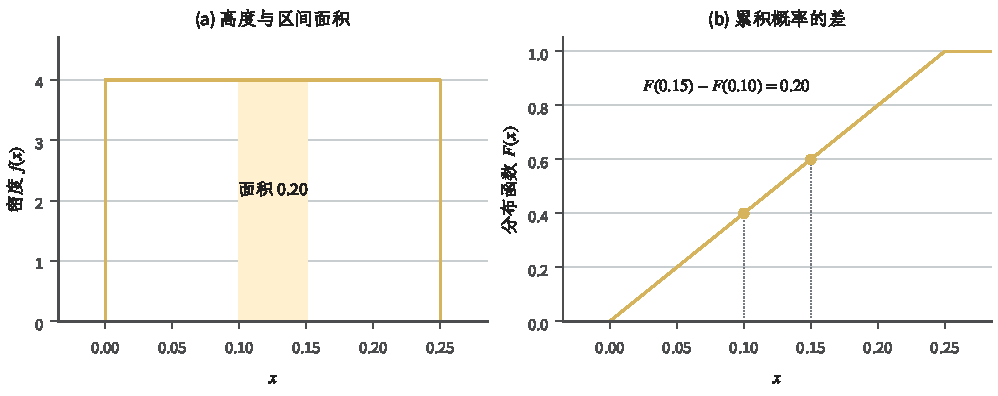
\includegraphics[width=\linewidth]{figures/math-preparation/probability-discrete/probability-density-cdf.pdf}
  \caption{区间\([0,1/4]\)上的均匀分布（解析式教学图）。左图阴影为\([0.10,0.15]\)的概率\(0.20\)，密度高度为\(4\)；右图的概率是\(F(0.15)-F(0.10)\)，两个端点本身均没有正概率质量。}
  \label{fig:probability-density-cdf}
\end{figure*}

\subsubsection{期望与分布积分}

对非负随机变量\(X\)，定义
\[ \mathbb{E}[X]
  =\int_{\Omega}X(\omega)\,\mathrm{d}\mathbb{P}(\omega). \]
对一般实随机变量，写\(X=X^+-X^-\)。当
\(\mathbb{E}[|X|]<\infty\)时，正负两部分积分都有限，此时称\(X\)可积，并定义
\(\mathbb{E}[X]=\mathbb{E}[X^+]-\mathbb{E}[X^-]\)。不要求可积便随意相减\(\infty-\infty\)没有意义。

期望只依赖\(X\)的分布。对可测函数\(g\)，只要\(g(X)\)非负或可积，就有
\begin{equation}
  \mathbb{E}[g(X)]
  =
  \int_{\mathbb{R}}g(x)\,\mathrm{d}\mathbb{P}_X(x).
  \label{eq:probability-lotus}
\end{equation}
离散时右侧是\(\sum_x g(x)p_X(x)\)，有密度时则是\(\int g(x)f_X(x)\,\mathrm{d}x\)。这条“无须先求\(g(X)\)分布”的积分公式，会反复用于矩、蒙特卡洛估计和分布变换。

式~\eqref{eq:probability-lotus}直接来自推送测度的定义。对指示函数
\(g=\mathbb{I}_B\)，等式两侧分别为
\(\mathbb{P}(X\in B)\)与\(\mathbb{P}_X(B)\)，所以相等。线性性把结论推广到非负简单函数；任取递增到非负可测\(g\)的简单函数列，再在两侧使用单调收敛定理，即得非负情形。可积实值函数则分别对\(g^+\)和\(g^-\)应用这一结论。这个证明同时说明，等式并不要求\(X\)有密度。

\begin{example}[带噪观测的平均目标]
\label{ex:probability-noisy-observation}
设未知信号为\(\theta\)，观测为
\[ Y=\theta+\varepsilon,
  \qquad\mathbb{E}[\varepsilon]=0. \]
只要\(\varepsilon\)可积，就有\(\mathbb{E}[Y]=\theta\)。这并未说明一次读数接近
\(\theta\)，也未说明多个读数的平均必然收敛；后者还需要抽样依赖关系和矩条件。概率模型先把目标写成分布下的平均，后续误差结论再回答有限观测能否逼近这个平均。
\end{example}

\subsection{绝对连续、密度与测度变换}
\label{sec:probability-radon-nikodym-change-measure}

熟悉的密度以Lebesgue测度为参照，概率质量函数以计数测度为参照。
两种写法共同的问题是：能否用一个参考测度下的权重表示另一个测度？
绝对连续排除参考测度完全看不到的正质量区域，Radon--Nikodym导数在这一前提下给出权重。
换测度随后复用同一个权重公式，而不必对每个分布重新推导积分。

\subsubsection{绝对连续与零集兼容性}

在有限集合上，两个概率表\((p_j)\)与\((q_j)\)可以逐项比较。若想用\(P\)下的样本计算\(Q\)下的平均，候选权重自然是\(q_j/p_j\)。但当\(p_j=0\)而\(q_j>0\)时，
\(P\)永远不会产生第\(j\)个结果，任何有限权重都无法补回这部分质量。

这一障碍在一般空间中由绝对连续刻画：参考测度看不到的集合，目标测度也不能给它
正质量。
\begin{definition}[测度的绝对连续]
\label{def:probability-absolute-continuity}
设\(\nu\)与\(\mu\)为同一可测空间\((\Omega,\mathcal{F})\)上的测度。若
\[ \mu(A)=0\Longrightarrow\nu(A)=0,
  \qquad\text{对所有 }A\in\mathcal{F}\text{成立}, \]
则称\(\nu\)对\(\mu\)\term{绝对连续}（absolute continuity），记作\(\nu\ll\mu\)。
\end{definition}
它只要求\(\mu\)的零集也是\(\nu\)的零集，并不表示\(\nu(A)\leq\mu(A)\)，
也不自动提供有界的密度比。

\subsubsection{有限分割上的密度表示}

先设\(\mu\)与\(\nu\)为有限测度，取有限可测分割
\(\Omega=A_1\mathbin{\dot\cup}\cdots\mathbin{\dot\cup}A_m\)，并假设\(\nu\ll\mu\)。
对\(\mu(A_j)>0\)的分块定义
\[ r(\omega)=\frac{\nu(A_j)}{\mu(A_j)},
  \qquad \omega\in A_j; \]
在\(\mu(A_j)=0\)的分块上令\(r=0\)。绝对连续性保证后一类分块也满足\(\nu(A_j)=0\)。因此，对任意由这些分块组成的事件\(A\)，
\[ \nu(A)=\int_A r\,\mathrm{d}\mu. \]
对在各分块上取有限实常数的函数\(g\)，逐项相加还给出
\begin{equation}
  \int_{\Omega}g\,\mathrm{d}\nu
  =
  \int_{\Omega}gr\,\mathrm{d}\mu.
  \label{eq:probability-finite-change-measure}
\end{equation}
一般定理要做的事，是在没有预先给定有限分块时构造同样的\(r\)
\scite{math-kallenberg2021probability}

\begin{theorem}[Radon--Nikodym定理]
\label{thm:probability-radon-nikodym}
设\(\mu\)与\(\nu\)是\((\Omega,\mathcal{F})\)上的\(\sigma\)有限测度，且
\(\nu\ll\mu\)。则存在非负可测函数\(r\)，使每个\(A\in\mathcal{F}\)都满足
\begin{equation}
  \nu(A)=\int_A r\,\mathrm{d}\mu.
  \label{eq:probability-rn-representation}
\end{equation}
函数\(r\)在\(\mu\)-几乎处处意义下唯一，记为\(r=\mathrm{d}\nu/\mathrm{d}\mu\)，称为\term{Radon--Nikodym导数}
（Radon--Nikodym derivative）。
\end{theorem}

\begin{proof}
先设\(\mu,\nu\)有限，并令\(\lambda=\mu+\nu\)。在线性空间
\(L^2(\lambda)\)上定义
\[
  T(f)=\int f\,\mathrm{d}\nu.
\]
由于\(\nu\leq\lambda\)，Cauchy--Schwarz不等式给出
\[
  |T(f)|
  \leq\int|f|\,\mathrm{d}\nu
  \leq\nu(\Omega)^{1/2}
       \left(\int f^2\,\mathrm{d}\nu\right)^{1/2}
  \leq\nu(\Omega)^{1/2}\lVert f\rVert_{L^2(\lambda)}.
\]
因此\(T\)是有界线性泛函。由第~\ref{chap:functional-analysis-and-approximation}章的Riesz表示定理，存在
\(g\in L^2(\lambda)\)，使
\[
  \int f\,\mathrm{d}\nu=\int fg\,\mathrm{d}\lambda,
  \qquad f\in L^2(\lambda).
\]
取\(f=\mathbb{I}_A\)可得\(\nu(A)=\int_Ag\,\mathrm{d}\lambda\)。若
\(A=\{g<0\}\)具有正测度，则对集合\(\{g\leq-1/k\}\)取指示函数会得到
\(\nu(\{g\leq-1/k\})<0\)的矛盾，故\(g\geq0\)几乎处处。又因为
\(\mu(A)=\lambda(A)-\nu(A)=\int_A(1-g)\,\mathrm{d}\lambda\geq0\)，同理有
\(g\leq1\)几乎处处。

令\(C=\{g=1\}\)。在\(C\)上有
\(\mu(C)=\int_C(1-g)\,\mathrm{d}\lambda=0\)，而\(\nu\ll\mu\)推出
\(\nu(C)=0\)。另一方面，\(\nu(C)=\int_Cg\,\mathrm{d}\lambda=\lambda(C)\)，所以
\(\lambda(C)=0\)。于是可以在其余部分定义
\[
  r=\frac{g}{1-g},
\]
并在\(C\)上任取值。由
\(\mathrm{d}\mu=(1-g)\,\mathrm{d}\lambda\)，对每个\(A\in\mathcal{F}\)都有
\[
  \int_A r\,\mathrm{d}\mu
  =\int_A\frac{g}{1-g}(1-g)\,\mathrm{d}\lambda
  =\int_Ag\,\mathrm{d}\lambda
  =\nu(A).
\]

若\(r_1,r_2\)都满足该表示，则对
\(A_k=\{r_1\geq r_2+1/k\}\)有
\[
  0=\int_{A_k}(r_1-r_2)\,\mathrm{d}\mu
  \geq\frac{1}{k}\mu(A_k),
\]
故\(\mu(A_k)=0\)。对\(k\)取并集得到\(r_1\leq r_2\)几乎处处；交换二者即得唯一性。

对\(\sigma\)有限的\(\mu,\nu\)，分别取有限测度覆盖并求交，可以把\(\Omega\)写成可数个互不相交、在两种测度下均有限的可测分块。在每个分块上使用上述构造，再把各块导数拼接，便得到全空间上的\(r\)。拼接后的表示可先对有限个分块验证，再由单调收敛推广到全部分块。
\end{proof}

这个证明先让\(\lambda=\mu+\nu\)同时支配两种测度，再把测度\(\nu\)表示为
\(L^2(\lambda)\)中的函数\(g\)。绝对连续性只用于排除\(g=1\)承载正质量，保证比值
\(g/(1-g)\)能够成为相对于\(\mu\)的密度。构造得到的是可测密度，并没有得到逐点上界。

\subsubsection{换测度公式与权重风险}

\begin{theorem}[换测度积分公式]
\label{thm:probability-change-measure-integral}
若\(\nu\ll\mu\)，\(r=\mathrm{d}\nu/\mathrm{d}\mu\)，则对每个非负可测函数\(g\)，
\[ \int g\,\mathrm{d}\nu
  =\int gr\,\mathrm{d}\mu. \]
只要\(g\)在\(\nu\)下可积，同一等式也对实值\(g\)成立。
\end{theorem}

\begin{proof}
对指示函数\(g=\mathbb{I}_A\)，结论就是Radon--Nikodym表示。由线性性，它对非负简单函数成立。任取非负可测\(g\)，选择简单函数\(g_n\uparrow g\)，分别在
\(\nu\)和\(\mu\)下使用单调收敛定理即可。对可积实值函数，再分别处理\(g^+\)与\(g^-\)。
\end{proof}

密度比存在、有界和具有有限二阶矩是三项不同条件。若\(P\ll Q\)，则\(w=\mathrm{d}P/\mathrm{d}Q\)存在且\(\mathbb{E}_Q[w]=1\)，但这不推出
\(\lVert w\rVert_\infty<\infty\)，也不推出\(\mathbb{E}_Q[w^2]<\infty\)。例如在\((0,1)\)上令\(Q\)为均匀分布，取
\[ w(x)=\frac{1}{2\sqrt{x}}. \]
它的积分为\(1\)，所以定义一个\(P\ll Q\)；但\(w\)无界，且\(\int_0^1w(x)^2\,\mathrm{d}x=\infty\)。换测度恒等式仍成立，使用该权重的蒙特卡洛估计却可能没有有限方差。

有限表可以直接核对权重方向。设参考分布\(Q\)在三个结果上的概率为
\((0.5,0.4,0.1)\)，目标分布\(P\)为\((0.2,0.3,0.5)\)，则
\[
  w=\frac{\mathrm{d}P}{\mathrm{d}Q}=(0.4,0.75,5).
\]
对取值\(g=(1,2,4)\)，有
\[
  \mathbb{E}_P[g]=2.8
  =0.5(0.4)(1)+0.4(0.75)(2)+0.1(5)(4)
  =\mathbb{E}_Q[wg].
\]
第三个结果在\(Q\)下少见，却在\(P\)下承载一半质量，所以产生大权重。若把参考概率
\(0.1\)改成\(0\)而保持目标概率\(0.5\)，则\(P\not\ll Q\)，任何重加权都无法从
\(Q\)样本恢复这部分目标质量。

图~\ref{fig:probability-importance-weights}显示，权重改变的是每个结果对平均的贡献，而不是把观测值\(g_j\)解释为概率。未加权平均为\(1.7\)，加权平均为\(2.8\)；第三个结果的贡献从\(0.4\)增至\(2\)，也预示它偶尔出现时会显著推动估计值。

\begin{figure*}[htbp]
  \centering
  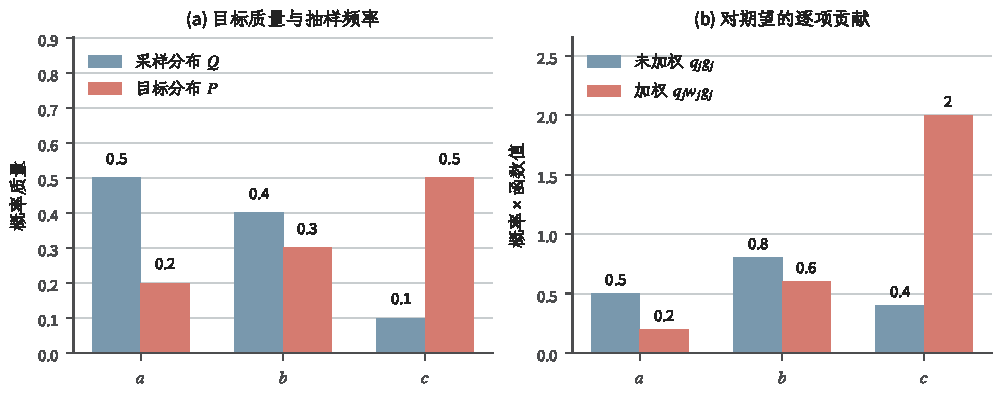
\includegraphics[width=\linewidth]{figures/math-preparation/probability-discrete/probability-importance-weights.pdf}
  \caption{三结果换测度的有限构造。左图比较采样分布\(Q\)与目标分布\(P\)，右图比较\(q_jg_j\)与\(q_jw_jg_j=p_jg_j\)。各柱从零起画；右图柱高之和分别为\(1.7\)和\(2.8\)，并非单点概率。}
  \label{fig:probability-importance-weights}
\end{figure*}

绝对连续性也决定几乎处处结论能否转移。若\(P\ll Q\)，且
\(|g|\leq M\)在\(Q\)下几乎处处成立，则违背上界的集合是\(Q\)-零集，因而也是
\(P\)-零集；同一上界在\(P\)下仍成立。反向转移需要\(Q\ll P\)，不能只凭
\(P\ll Q\)得到。若\(|g|\leq B\)，则
\[
  \mathbb{E}_Q[w^2g^2]\leq B^2\mathbb{E}_Q[w^2],
\]
所以权重二阶矩有限是有界被积函数获得有限重加权方差的充分条件。把权重截为
\(w_c=\min\{w,c\}\)会限制波动，但
\(\mathbb{E}_Q[w_cg]\)与\(\mathbb{E}_P[g]\)之差为
\(-\mathbb{E}_Q[(w-c)_+g]\)，一般不为零。

\subsection{联合、边缘与条件分布}
\label{sec:probability-joint-marginal-conditional}

换测度在同一积分对象上改变概率权重；条件化则根据已经观察到的变量重新描述未知结果。
离散条件概率可以直接相除，连续变量的单点通常没有正概率，不能沿用同一个分母解释。
概率核把“对每个条件值给一个分布”组织成可测对象，正则条件分布的存在条件由此成为必要问题。

\subsubsection{联合分布与边缘分布}

随机向量\((X,Y)\)的联合分布是映射\(\omega\mapsto(X(\omega),Y(\omega))\)在乘积空间上诱导的概率测度。离散情形中，
联合质量\(p_{X,Y}(x,y)\)给出完整表格，边缘分布由求和消去另一坐标：
\[ p_X(x)=\sum_y p_{X,Y}(x,y),
  \qquad p_Y(y)=\sum_x p_{X,Y}(x,y). \]
若联合分布有密度，则相应运算变为
\[ f_X(x)=\int f_{X,Y}(x,y)\,\mathrm{d}y. \]
一般情形不需要质量函数或密度。记坐标投影为\(\pi_X(x,y)=x\)，则边缘分布就是联合分布经\(\pi_X\)的推送：
\[
  \mathbb{P}_X(A)
  =\mathbb{P}_{(X,Y)}(A\times\mathcal{Y}).
\]
对非负可测函数\(g\)，式~\eqref{eq:probability-lotus}给出
\[
  \int g(x)\,\mathbb{P}_X(\mathrm{d}x)
  =
  \int g\bigl(\pi_X(x,y)\bigr)\,
       \mathbb{P}_{(X,Y)}(\mathrm{d}x,\mathrm{d}y).
\]
若联合分布有密度，再对右侧使用Tonelli定理，才得到对\(y\)积分的边缘密度公式。因而“边缘化”首先是测度推送，求和或积分只是它在特定参考测度下的表达。

边缘化会丢掉变量如何共同变化的信息。两个不同联合分布可以拥有完全相同的两个边缘分布。

当\(p_X(x)>0\)时，离散条件质量定义为
\[ p_{Y\mid X}(y\mid x)
  =\frac{p_{X,Y}(x,y)}{p_X(x)}. \]
因此有乘法公式
\[ p_{X,Y}(x,y)=p_X(x)p_{Y\mid X}(y\mid x). \]
若\(p_Y(y)>0\)，把联合质量按另一顺序分解便得到Bayes公式
\begin{equation}
  p_{X\mid Y}(x\mid y)
  =
  \frac{p_{Y\mid X}(y\mid x)p_X(x)}
       {\sum_{x'}p_{Y\mid X}(y\mid x')p_X(x')}.
  \label{eq:probability-discrete-bayes}
\end{equation}
分母是观测\(y\)的边缘概率，既负责归一化，也要求观测并非零概率事件。

连续密度公式是同一分解的特例。若\((X,Y)\)相对于乘积参考测度有联合密度
\(f_{X,Y}\)，且\(0<f_X(x)<\infty\)，则
\[
  f_{Y\mid X}(y\mid x)
  =\frac{f_{X,Y}(x,y)}{f_X(x)}
\]
非负并对\(y\)积分为\(1\)。它满足
\(f_{X,Y}(x,y)=f_X(x)f_{Y\mid X}(y\mid x)\)。在
\(f_X(x)=0\)或\(f_X(x)=\infty\)的点上，不能使用这个比值；这些点构成\(\mathbb P_X\)-零测集。条件核在该零测集上可统一指定一个固定概率测度，而不改变联合分布。这里选用由联合密度积分得到的边缘密度版本；任意修改过的密度版本也只能保证相应等式几乎处处成立。

\begin{example}[有限候选经过带噪观测更新]
\label{ex:probability-finite-candidate-bayes}
设信号只可能是\(\Theta\in\{-1,1\}\)，先验概率均为\(1/2\)。传感器以概率\(0.8\)报告正确符号。观测\(Y=1\)后，
\[ \mathbb{P}(\Theta=1\mid Y=1)
  =\frac{0.8\times0.5}{0.8\times0.5+0.2\times0.5}=0.8. \]
观测并未把候选集合改成一个确定点，而是改变了两个候选的相对权重。若某个观测在所有
候选下概率都为零，公式分母为零，条件分布不能靠这个比值定义。
\end{example}

\subsubsection{概率核与条件化的可测性}

当条件变量连续时，事件\(\{X=x\}\)常有零概率，直接相除不再可行。需要把“每个条件值对应一个分布”组织成能继续积分的对象。
\begin{definition}[概率核]
  \label{def:probability-kernel}
  给定可测空间\((\mathcal X,\mathcal A)\)、\((\mathcal Y,\mathcal B)\)，\term{概率核}（probability kernel）是映射
  \[ K:\mathcal X\times\mathcal B\to[0,1], \]
  满足：对每个\(x\in\mathcal X\)，\(K(x,\cdot)\)是\((\mathcal Y,\mathcal B)\)上的概率测度；对每个\(B\in\mathcal B\)，\(x\mapsto K(x,B)\)是\(\mathcal A\)-可测函数。
\end{definition}
第一项保证每个条件值给出合法分布，
第二项保证再对\(X\)积分是合法运算。

可测并不等于连续。例如取\(X\sim\mathcal N(0,1)\)、\(Y=\mathbb I\{X\geq0\}\)，则\(K(x,\{1\})=\mathbb I\{x\geq0\}\)是合法概率核在事件\(\{1\}\)上的取值，却在\(x=0\)处跳变。条件值\(x\)可以连续取值，条件分布随\(x\)变化仍可不连续。

\begin{definition}[正则条件分布]
  \label{def:probability-regular-conditional-distribution}
若概率核\(K\)对所有\(A\in\mathcal A\)、\(B\in\mathcal B\)满足
\begin{equation}
  \mathbb{P}(X\in A,Y\in B)
  =
  \int_A K(x,B)\,\mathbb{P}_X(\mathrm{d}x),
  \label{eq:probability-regular-conditional-kernel}
\end{equation}
就把\(K(x,\cdot)\)称为\(Y\)给定\(X=x\)的一个\term{正则条件分布}（regular conditional distribution）。
\end{definition}
对每个固定可测集\(B\)，两个版本的\(K(x,B)\)在\(\mathbb P_X\)-几乎处处意义下相同；若\(\mathcal Y\)是下面的标准Borel空间，还可选取一个共同零测集，使其外的条件概率测度相同。零概率条件点上的取值通常不能由联合分布唯一决定。

\subsubsection{正则条件分布的存在条件}

逐个条件事件的概率能够定义，并不保证它们能拼成一个共同的概率核。下面的可测空间条件为这种拼接提供保证。
\begin{definition}[Polish空间]
  \label{def:probability-polish-space}
拓扑空间若存在一个诱导该拓扑的完备、可分度量，就称为Polish空间。可分表示含有可数稠密子集；完备性表示该度量下每个Cauchy序列都收敛到空间中的点。
\end{definition}
欧氏空间就是一个例子。这里既需要能用可数对象逼近，也需要极限仍落在所研究的空间内；标准Borel空间只保留这种空间的可测结构。
\begin{definition}[标准Borel空间]
  \label{def:probability-standard-borel-space}
  可测空间称为\term{标准Borel空间}（standard Borel space），若它与某个完备可分度量空间的Borel子集可测同构，即存在双射，且该双射及其逆映射都可测。
\end{definition}
“可分”表示度量空间含有可数稠密子集。若\(X\)与\(Y\)的状态空间都是标准Borel空间，则上述正则条件分布存在。实数空间、欧氏空间、可数集合以及配备适当Borel结构的常见可分函数空间都属于这一范围。

这一存在结论依赖可数生成结构与条件期望。下一小节定义条件期望以后，再说明逐个事件上的条件平均如何组成同一个概率核。

在完全一般的可测空间上，正则条件分布可能不存在。此时条件期望仍可相对于子\(\sigma\)代数定义，但不能未经说明就把它写成每个点\(x\)上的条件密度。后续模型
通常工作在标准Borel空间中；使用\(p(y\mid x)\)时，应同时确认密度所依赖的参考测度及其适用的几乎处处范围。

\subsection{期望、方差与条件期望}
\label{sec:probability-expectation-conditional-expectation}

\subsubsection{均值、方差与协方差}

可积随机变量的均值记作\(\mu_X=\mathbb{E}[X]\)。若\(\mathbb{E}[X^2]<\infty\)，其方差为
\[ \operatorname{Var}(X)
  =\mathbb{E}\bigl[(X-\mu_X)^2\bigr]=\mathbb{E}[X^2]-\mu_X^2. \]
对二阶可积的\(X,Y\)，协方差为
\[ \operatorname{Cov}(X,Y)
  =\mathbb{E}\bigl[(X-\mathbb{E}X)(Y-\mathbb{E}Y)\bigr]. \]
Cauchy--Schwarz不等式保证它有限。方差满足
\[ \operatorname{Var}(aX+b)=a^2\operatorname{Var}(X), \]
而
\[ \operatorname{Var}(X+Y)
  =\operatorname{Var}(X)+\operatorname{Var}(Y)+2\operatorname{Cov}(X,Y). \]
只有协方差为零时，方差才直接相加；独立是协方差为零的充分条件，但通常不是必要条件。

\subsubsection{条件期望与信息约束}

子\(\sigma\)代数\(\mathcal{G}\subseteq\mathcal{F}\)表示当前可用信息。预测值必须只使用这些信息，又应在每个可识别的分组内保持平均值。
\begin{definition}[观测生成的信息]
  \label{def:probability-generated-information}
若\(X:\Omega\to(\mathcal X,\mathcal A)\)是随机变量，记
\(\sigma(X)=\{X^{-1}(A):A\in\mathcal A\}\)。它是使\(X\)可测的最小\(\sigma\)代数，表示仅观察\(X\)能够区分的事件。多个观测生成的信息是包含它们全部可测逆像的最小\(\sigma\)代数。
\end{definition}
例如只观察分组编号，就不能在同一组内区分两个原始结果。写\(\mathbb E[Y\mid X]\)时，真正限制答案的信息是\(\sigma(X)\)，不是单个零概率事件\(\{X=x\}\)。
\begin{definition}[条件期望]
  \label{def:probability-conditional-expectation}
对\(X\in L^1(\mathbb P)\)，\term{条件期望}（conditional expectation）
\(\mathbb{E}[X\mid\mathcal{G}]\)是满足下列两项条件的可积随机变量\(Z\)：
\[ Z\text{ 对 }\mathcal{G}\text{ 可测},
  \qquad\int_A Z\,\mathrm{d}\mathbb{P}=\int_A X\,\mathrm{d}\mathbb{P}\quad(A\in\mathcal{G}). \]
\end{definition}
第一项要求答案只能使用\(\mathcal{G}\)中的信息，第二项要求它在每个可由当前信息识别的事件上保留\(X\)的平均
\scite{math-kallenberg2021probability}

\begin{theorem}[条件期望的存在与唯一性]
\label{thm:probability-conditional-expectation-existence}
若\(X\in L^1(\mathbb{P})\)，则\(\mathbb{E}[X\mid\mathcal{G}]\)存在，并在几乎处处意义下唯一。
\end{theorem}

\begin{proof}
先设\(X\geq0\)。在\((\Omega,\mathcal{G})\)上定义有限测度
\[ \nu(A)=\int_A X\,\mathrm{d}\mathbb{P}. \]
若\(\mathbb{P}(A)=0\)，则\(\nu(A)=0\)，所以\(\nu\ll\mathbb{P}|_{\mathcal{G}}\)。Radon--Nikodym定理给出非负、
\(\mathcal{G}\)-可测的\(Z\)，使\(\nu(A)=\int_A Z\,\mathrm{d}\mathbb{P}\)。对一般可积\(X\)，分别对
\(X^+\)与\(X^-\)使用这一构造并取差，即得存在性。

若\(Z_1,Z_2\)都满足定义，令\(D=Z_1-Z_2\)。对每个\(A\in\mathcal{G}\)，\(\int_A D\,\mathrm{d}\mathbb{P}=0\)。若
\(\mathbb{P}(D>0)>0\)，则某个集合\(A_k=\{D\geq1/k\}\)具有正概率，从而
\[ \int_{A_k}D\,\mathrm{d}\mathbb{P}
  \geq\frac{1}{k}\mathbb{P}(A_k)>0, \]
产生矛盾。因此\(D\leq0\)几乎处处。交换\(Z_1,Z_2\)可得\(D\geq0\)几乎处处，故二者几乎处处相等。
\end{proof}

若\(X\)本来就对\(\mathcal{G}\)可测，则\(\mathbb{E}[X\mid\mathcal{G}]=X\)几乎处处。若\(X\)与\(\mathcal{G}\)
独立，则条件期望等于常数\(\mathbb{E}[X]\)。若\(U\)有界且\(\mathcal{G}\)-可测，则
\begin{equation}
  \mathbb{E}[UX\mid\mathcal{G}]
  =
  U\mathbb{E}[X\mid\mathcal{G}].
  \label{eq:probability-taking-out-known-factor}
\end{equation}
可积的非有界\(U\)需要另外核对乘积可积性，不能仅凭“已知量可提出”略去条件。

有限分组把抽象定义化成逐组平均。若
\(A_1,\ldots,A_m\)是有限可测分割，
\(\mathcal{G}=\sigma(A_1,\ldots,A_m)\)，且每个
\(\mathbb{P}(A_j)>0\)，则
\begin{equation}
  \mathbb{E}[X\mid\mathcal{G}]
  =
  \sum_{j=1}^{m}
  \frac{\mathbb{E}[X\mathbb{I}_{A_j}]}
       {\mathbb{P}(A_j)}
  \mathbb{I}_{A_j}.
  \label{eq:probability-finite-partition-conditional-expectation}
\end{equation}
若某个分组概率为零，该组上的取值可以任意指定，因为条件期望只在几乎处处意义下唯一。

表~\ref{tab:probability-finite-partition-predictions}给出一个可复核例子。令
\(\mathcal{G}\)只能区分
\(A=\{\omega_1,\omega_2\}\)与
\(B=\{\omega_3,\omega_4\}\)。不使用分组信息时，最佳常数预测是
\(U_0=\mathbb{E}X=3.4\)；规则\(U_{\mathrm{grp}}\)虽然按组取值，却随意地在
\(A,B\)上分别预测\(0,4\)；条件均值\(m=\mathbb{E}[X\mid\mathcal{G}]\)则在两组
上分别等于\(1.2,5.6\)。
\begin{table}[htbp]
  \centering
  \small
  \begin{tabular}{ccccccc}
    \toprule
    结果 & 概率 & \(X\) & 分组 & \(U_0\) & \(U_{\mathrm{grp}}\) & \(m\) \\
    \midrule
    \(\omega_1\) & \(0.2\) & \(0\) & \(A\) & \(3.4\) & \(0\) & \(1.2\) \\
    \(\omega_2\) & \(0.3\) & \(2\) & \(A\) & \(3.4\) & \(0\) & \(1.2\) \\
    \(\omega_3\) & \(0.1\) & \(4\) & \(B\) & \(3.4\) & \(4\) & \(5.6\) \\
    \(\omega_4\) & \(0.4\) & \(6\) & \(B\) & \(3.4\) & \(4\) & \(5.6\) \\
    \midrule
    \multicolumn{4}{r}{平方风险\(\ \mathbb{E}[(X-U)^2]\)} &
    \(5.64\) & \(2.80\) & \(0.80\) \\
    \bottomrule
  \end{tabular}
  \caption{有限分组下的三类预测。分组信息使预测可以随\(A,B\)变化，但只有逐组条件
  均值在全部\(\mathcal{G}\)-可测平方可积预测中达到最小平方风险。}
  \label{tab:probability-finite-partition-predictions}
\end{table}
三列风险依次说明不同问题：获得分组信息可以优于无信息常数，但使用信息本身不保证已经
最优；式~\eqref{eq:probability-finite-partition-conditional-expectation}还要在每组
内选择正确的条件平均。

构造思路可以从可数生成族看清。先在\(\mathcal{Y}\)的一个可数、能区分概率测度的集合族上，对每个\(B\)构造
\(\mathbb{P}(Y\in B\mid\sigma(X))\)；再选取这些条件期望关于\(X\)的可测版本。在去掉一个共同零测集后，这些数值满足有限可加性和连续性，扩张定理把它们唯一延拓为
\(\mathcal{Y}\)上的概率测度。标准Borel结构提供的可数性和可分性，正是把逐个事件的版本整理成同一个概率核所需的条件。

\subsubsection{塔式性质与全期望}

\begin{theorem}[塔式性质]
\label{thm:probability-tower-property}
若\(X\in L^1\)，且\(\mathcal{H}\subseteq\mathcal{G}\subseteq\mathcal{F}\)，则
\[ \mathbb{E}\bigl[\mathbb{E}[X\mid\mathcal{G}]
  \mid\mathcal{H}\bigr]=\mathbb{E}[X\mid\mathcal{H}] \]
几乎处处成立。
\end{theorem}

\begin{proof}
左侧对\(\mathcal{H}\)可测。对任意\(A\in\mathcal{H}\)，由于\(A\in\mathcal{G}\)，条件期望定义给出
\[
  \int_A
  \mathbb{E}\bigl[\mathbb{E}[X\mid\mathcal{G}]
  \mid\mathcal{H}\bigr]\,\mathrm{d}\mathbb{P}
  =
  \int_A\mathbb{E}[X\mid\mathcal{G}]\,\mathrm{d}\mathbb{P}
  =
  \int_A X\,\mathrm{d}\mathbb{P}.
\]
左侧因而满足\(X\)关于\(\mathcal{H}\)的条件期望定义，唯一性给出结论。
\end{proof}

取\(\mathcal{H}=\{\varnothing,\Omega\}\)，便得到\term{全期望公式}（law of total expectation）
\begin{equation}
  \mathbb{E}\bigl[\mathbb{E}[X\mid\mathcal{G}]\bigr]
  =
  \mathbb{E}[X].
  \label{eq:probability-total-expectation}
\end{equation}
这说明条件化改变可用信息，却不改变再平均后的总体均值。

\subsubsection{全方差分解}

设\(X\in L^2\)，记\(m=\mathbb{E}[X\mid\mathcal{G}]\)。分解
\[ X-\mathbb{E}X=(X-m)+(m-\mathbb{E}X). \]
在展开平方前，需要先确认条件均值仍然二阶可积。对凸函数\(u\mapsto u^2\)使用条件
Jensen不等式，有
\[
  |m|^2
  \leq
  \mathbb{E}[X^2\mid\mathcal{G}].
\]
再取期望并使用全期望公式，得到
\[
  \mathbb{E}[m^2]\leq\mathbb{E}[X^2]<\infty.
\]
因此\(m\in L^2\)，上面分解中的两项都二阶可积，其乘积由Cauchy--Schwarz不等式保证可积。又因为第二项对
\(\mathcal{G}\)可测，而\(\mathbb{E}[X-m\mid\mathcal{G}]=0\)，所以交叉项期望为
\[ \mathbb{E}\bigl[(X-m)(m-\mathbb{E}X)\bigr]
  =\mathbb{E}\left[(m-\mathbb{E}X)\mathbb{E}[X-m\mid\mathcal{G}]\right]=0. \]
展开平方得到\term{全方差公式}（law of total variance）
\begin{equation}
  \operatorname{Var}(X)
  =
  \mathbb{E}\bigl[\operatorname{Var}(X\mid\mathcal{G})\bigr]
  +
  \operatorname{Var}\bigl(\mathbb{E}[X\mid\mathcal{G}]\bigr),
  \label{eq:probability-total-variance}
\end{equation}
其中
\[ \operatorname{Var}(X\mid\mathcal{G})
  =\mathbb{E}\bigl[(X-m)^2\mid\mathcal{G}\bigr]. \]
第一项是获得\(\mathcal{G}\)后仍无法解释的平均波动，第二项是不同信息状态之间的可解释波动。

\subsubsection{条件期望的平方损失最优性}

\begin{theorem}[条件均值的平方损失最优性]
\label{thm:probability-conditional-mean-l2-projection}
设\(X\in L^2(\mathbb{P})\)。在所有\(\mathcal{G}\)-可测且二阶可积的随机变量\(U\)中，
\[ m=\mathbb{E}[X\mid\mathcal{G}] \]
唯一地在几乎处处意义下最小化\(\mathbb{E}[(X-U)^2]\)。
\end{theorem}

\begin{proof}
\(L^2(\mathcal{G})\)是\(L^2(\mathcal{F})\)的闭线性子空间，上文的条件Jensen不等式已经说明
\(m\in L^2(\mathcal{G})\)。对每个\(U\in L^2(\mathcal{G})\)，Cauchy--Schwarz不等式保证
\((X-m)U\)可积，因而可以提出已知因子并使用塔式性质，得到
\[ \mathbb{E}[(X-m)U]
  =\mathbb{E}\left[U\mathbb{E}[X-m\mid\mathcal{G}]\right]=0. \]
所以\(X-m\)与整个\(L^2(\mathcal{G})\)正交。定理~\ref{thm:functional-hilbert-projection}说明\(m\)是\(X\)到该闭子空间的正交投影。也可直接展开
\begin{equation}
  \mathbb{E}[(X-U)^2]
  =
  \mathbb{E}[(X-m)^2]
  +
  \mathbb{E}[(m-U)^2],
  \label{eq:probability-pythagorean-prediction}
\end{equation}
交叉项因正交性消失。第二项非负，且仅当\(U=m\)几乎处处时为零。
\end{proof}

条件期望的存在只需要\(X\in L^1\)，这时它由Radon--Nikodym导数给出。“正交投影”和平方损失最优性则需要\(X\in L^2\)。若二阶矩无限，条件期望仍可能
存在，但不能使用Hilbert空间几何或有限平方风险。

\subsubsection{条件换测度}

设\(Q\ll P\)，并记\(L=\mathrm{d}Q/\mathrm{d}P\)。对\(X\in L^1(Q)\)，在\(\mathbb{E}_P[L\mid\mathcal{G}]>0\)处有
\begin{equation}
  \mathbb{E}_Q[X\mid\mathcal{G}]
  =
  \frac{\mathbb{E}_P[LX\mid\mathcal{G}]}
       {\mathbb{E}_P[L\mid\mathcal{G}]}.
  \label{eq:probability-conditional-change-measure}
\end{equation}
为验证这个候选变量确实是条件期望，记
\[
  D=\mathbb{E}_P[L\mid\mathcal{G}],
  \qquad
  N=\mathbb{E}_P[LX\mid\mathcal{G}],
\]
并在\(\{D>0\}\)上令\(Z=N/D\)，在\(\{D=0\}\)上令\(Z=0\)。分母零集在\(Q\)下可以忽略，因为
\[
  Q(D=0)
  =
  \mathbb{E}_P[L\mathbb{I}\{D=0\}]
  =
  \mathbb{E}_P[D\mathbb{I}\{D=0\}]
  =0.
\]
条件期望的单调性还给出
\[
  |N|
  \leq
  \mathbb{E}_P[L|X|\mid\mathcal{G}].
\]
在\(\{D=0\}\)上，非负变量\(L\mathbb{I}\{D=0\}\)的期望为零，因而\(L=0\)几乎处处。于是
\[
  \mathbb{E}_P\left[
    \mathbb{E}_P[L|X|\mid\mathcal{G}]
    \mathbb{I}\{D=0\}
  \right]
  =
  \mathbb{E}_P[L|X|\mathbb{I}\{D=0\}]
  =0,
\]
上面的条件三角不等式进而说明\(N=0\)在\(\{D=0\}\)上几乎处处成立。因此\(DZ=N\)几乎处处，而且
\[
  \begin{aligned}
    \mathbb{E}_Q|Z|
    &=
    \mathbb{E}_P[L|Z|]
    =
    \mathbb{E}_P[D|Z|]\\
    &=
    \mathbb{E}_P\bigl[|N|\mathbb{I}\{D>0\}\bigr]
    \leq
    \mathbb{E}_P[L|X|]
    =
    \mathbb{E}_Q|X|<\infty.
  \end{aligned}
\]
这里把\(\mathcal{G}\)-可测的非负因子\(|Z|\)提出条件期望，可以由有界截断和单调收敛得到。候选变量的可积性建立后，对
\(A\in\mathcal{G}\)可合法地计算
\[
  \begin{aligned}
    \int_A Z\,\mathrm{d}Q
    &=
    \int_A ZL\,\mathrm{d}P
    =
    \int_A Z\mathbb{E}_P[L\mid\mathcal{G}]\,\mathrm{d}P\\
    &=
    \int_A \mathbb{E}_P[LX\mid\mathcal{G}]\,\mathrm{d}P
    =
    \int_A LX\,\mathrm{d}P
    =
    \int_A X\,\mathrm{d}Q.
  \end{aligned}
\]
因此\(Z\)满足\(X\)在\(Q\)下关于\(\mathcal{G}\)的条件期望定义。公式\eqref{eq:probability-conditional-change-measure}是Bayes更新的一般测度形式；
分母零集与候选变量可积性都需要像上面这样核对。

用有限分组可以看出分母为何不可省略。设参考分布\(P\)把四个结果
\(\omega_1,\ldots,\omega_4\)分别赋予概率\((0.4,0.1,0.1,0.4)\)，目标分布
\(Q\)赋予\((0.1,0.4,0.2,0.3)\)。令信息\(\mathcal{G}\)只区分
\(A=\{\omega_1,\omega_2\}\)和\(A^{\mathsf c}\)，并令
\(X=(0,1,0,1)\)。权重\(L\)在四点上的值为\((0.25,4,2,0.75)\)。在\(A\)内，
\[
  \mathbb{E}_P[LX\mid\mathcal{G}]
  =\frac{0.4}{0.5}=0.8,\qquad
  \mathbb{E}_P[L\mid\mathcal{G}]
  =\frac{0.1+0.4}{0.5}=1,
\]
所以目标条件均值为\(0.8\)，与
\(\mathbb{E}_Q[X\mid A]=0.4/(0.1+0.4)\)一致。直接用某个无条件权重乘
\(\mathbb{E}_P[X\mid A]=0.2\)不会得到目标条件均值；条件化后必须在每个信息分组内重新归一化。

\subsection{独立与条件独立}
\label{sec:probability-moments-independence}

\subsubsection{独立、不相关与非线性依赖}

若随机变量\(X,Y\)满足
\[ \mathbb{P}(X\in A,Y\in B)
  =\mathbb{P}(X\in A)\mathbb{P}(Y\in B) \]
对所有Borel集合\(A,B\)成立，就称二者\term{独立}（independent）。独立意味着所有可积可分函数都满足
\(\mathbb{E}[g(X)h(Y)]=\mathbb{E}[g(X)]\mathbb{E}[h(Y)]\)。
证明从指示函数开始：独立性正好说明结论对
\(g=\mathbb{I}_A\)、\(h=\mathbb{I}_B\)成立。线性性把它推广到简单函数，随后分别用单调收敛处理非负函数，再分解正负部分处理乘积可积的实值函数。这里必须要求相关积分有定义，不能把两个发散期望形式相乘。

协方差只检查中心化变量的一次乘积。令\(X\)在\([-1,1]\)上均匀分布，并取\(Y=X^2\)。对称性给出
\[ \operatorname{Cov}(X,Y)
  =\mathbb{E}[X^3]-\mathbb{E}[X]\mathbb{E}[X^2]=0, \]
但\(Y\)由\(X\)完全决定；知道\(X\)便能确定\(Y\)，所以二者不独立。零协方差只排除了线性二阶关联。

\subsubsection{条件独立及其运算规则}

\begin{definition}[条件独立]
  \label{def:probability-conditional-independence}
  给定随机变量\(X,Y,Z\)，若对\(X,Y\)取值空间中的所有可测集合\(A,B\)，
\[ \mathbb{P}(X\in A,Y\in B\mid Z)
  =\mathbb{P}(X\in A\mid Z)\mathbb{P}(Y\in B\mid Z) \]
几乎处处成立，就称\(X\)与\(Y\)在给定\(Z\)时条件独立，记作
\(X\perp Y\mid Z\)。
\end{definition}
它表示\(Z\)已知以后，\(X\)不再提供关于\(Y\)的额外分布信息；这不意味着去掉\(Z\)后仍独立。

条件独立满足以下常用规则：
\[
\begin{aligned}
  X\perp Y\mid Z
  &\Longrightarrow Y\perp X\mid Z
  &&\text{（对称性）},\\
  X\perp(Y,W)\mid Z
  &\Longrightarrow X\perp Y\mid Z
  &&\text{（分解）},\\
  X\perp(Y,W)\mid Z
  &\Longrightarrow X\perp Y\mid Z,W
  &&\text{（弱并）},\\
  X\perp Y\mid Z,\quad X\perp W\mid Y,Z
  &\Longrightarrow X\perp(Y,W)\mid Z
  &&\text{（收缩）}.
\end{aligned}
\]
这些规则可由条件核的乘积分解逐项验证。交性质
\[ X\perp Y\mid Z,W,\quad
  X\perp W\mid Z,Y\Longrightarrow X\perp(Y,W)\mid Z \]
并非无条件成立；严格为正的有限离散联合质量是一个常用充分条件。若分布把质量集中在
低维约束上，零概率组合会阻断所需的消元步骤。

\begin{lemma}[严格正离散分布的交性质]
  \label{lem:probability-positive-intersection}
  设$I$为有限索引集，每个$i\in I$对应取值于有限非空状态空间$\mathcal{X}_i$的随机变量$X_i$。令$p$为$\bm{X}=(X_i)_{i\in I}$在乘积状态空间$\mathcal{X}=\prod_{i\in I}\mathcal{X}_i$上的联合质量函数，且$p(\bm{x})>0$对所有$\bm{x}\in\mathcal{X}$成立。对两两不交的索引集$A,B,C,D\subseteq I$，若
  \[
    \bm{X}_A\perp\bm{X}_B\mid(\bm{X}_C,\bm{X}_D),
    \qquad
    \bm{X}_A\perp\bm{X}_D\mid(\bm{X}_C,\bm{X}_B),
  \]
  则
  \[
    \bm{X}_A\perp(\bm{X}_B,\bm{X}_D)\mid\bm{X}_C.
  \]
\end{lemma}

\begin{proof}
严格正性保证以下每个条件概率都有定义。对任意取值$\bm{a},\bm{b},\bm{c},\bm{d}$，两个前提分别给出
\[
  p(\bm{a}\mid\bm{b},\bm{c},\bm{d})
  =p(\bm{a}\mid\bm{c},\bm{d}),
  \qquad
  p(\bm{a}\mid\bm{b},\bm{c},\bm{d})
  =p(\bm{a}\mid\bm{b},\bm{c}).
\]
因此$p(\bm{a}\mid\bm{c},\bm{d})=p(\bm{a}\mid\bm{b},\bm{c})$对每个$\bm{b},\bm{d}$成立。固定任意基准值$\bm{b}^{\circ}$，右侧等于$q(\bm{a},\bm{c})=p(\bm{a}\mid\bm{b}^{\circ},\bm{c})$，不再依赖$\bm{b}$或$\bm{d}$。对$(\bm{b},\bm{d})$关于$p(\bm{b},\bm{d}\mid\bm{c})$求和可得$q(\bm{a},\bm{c})=p(\bm{a}\mid\bm{c})$，故$p(\bm{a}\mid\bm{b},\bm{c},\bm{d})=p(\bm{a}\mid\bm{c})$，这正是所需的条件独立性。
\end{proof}
严格正性使上面证明能在固定\(\bm c\)后独立改变\(\bm b\)和\(\bm d\)。若只支持部分组合，这一步会失败。一个反例是\(X=Y=W=B\)，其中\(B\)为非退化Bernoulli变量，\(Z\)取常数。给定\(W\)后\(X,Y\)都确定，所以\(X\perp Y\mid W\)；给定\(Y\)后也有\(X\perp W\mid Y\)。但\(X\)与\((Y,W)\)显然不独立，因为后者直接给出\(X\)。两个条件独立前提因而不能在这类带零概率配置的分布上推出交性质。

以分解和收缩为例可以看清这些规则使用了什么。若
\(X\perp(Y,W)\mid Z\)，则对任意可测集合\(A,B,C\)，条件核满足
\[
  K_{X,Y,W\mid Z}(A,B,C\mid z)
  =K_{X\mid Z}(A\mid z)K_{Y,W\mid Z}(B,C\mid z).
\]
令\(C\)取全集便得到
\(K_{X,Y\mid Z}=K_{X\mid Z}K_{Y\mid Z}\)，这就是分解规则。对收缩规则，假设
\[
  K_{X,Y\mid Z}=K_{X\mid Z}K_{Y\mid Z},
  \qquad
  K_{X,W\mid Y,Z}=K_{X\mid Y,Z}K_{W\mid Y,Z}.
\]
第一个条件还给出
\(K_{X\mid Y,Z}=K_{X\mid Z}\)的一个版本。沿条件乘法公式相乘可得
\[
  K_{X,Y,W\mid Z}
  =K_{X\mid Z}K_{Y\mid Z}K_{W\mid Y,Z}
  =K_{X\mid Z}K_{Y,W\mid Z},
\]
即\(X\perp(Y,W)\mid Z\)。所有等式都按相应条件变量分布的几乎处处意义理解。概率图模型部分会在这些概率规则之上另加图分离语义；图上没有边本身并不是这里定义的条件独立证明。

多元高斯分布是一个特殊情形：联合高斯随机向量的两个子向量若协方差为零，则它们独立；条件高斯中的条件协方差为零也对应条件独立。这个结论依赖高斯
密度由一、二阶矩完全确定，不能推广到一般分布。

\section{分布族与随机变换}
\label{sec:probability-families-transformations}

共同的概率对象确定后，本节给出可计算的具体分布，并研究组合变量与改变坐标后的分布。
常用分布提供建模部件，线性变换、条件化和混合说明这些部件怎样组成联合模型。
计算结果时仍要返回上一节核对参考测度、支持与条件化对象。

\subsection{用矩与变换函数描述分布}
\label{sec:probability-moment-transforms}

均值和方差便于计算，却不足以区分许多分布。若关心偏斜、尾部或独立和的分布变化，需要在这两个摘要之外保留信息：高阶矩增加摘要阶数，生成函数则把一系列摘要组织到一个函数中。

若\(\mathbb{E}[|X|^k]<\infty\)，则\(\mathbb{E}[X^k]\)称为\(k\)阶原点矩，
\(\mathbb{E}[(X-\mathbb{E}X)^k]\)称为\(k\)阶中心矩。三阶中心矩反映不对称性，四阶中心矩反映尾部与峰度，但有限低阶矩通常不能唯一确定分布。

\begin{definition}[矩母函数与累积量生成函数]
  \label{def:probability-moment-generating-functions}
设\(X\)为实随机变量。若存在\(\delta>0\)，使\(\mathbb E e^{tX}<\infty\)对全部\(|t|<\delta\)成立，则在该邻域上定义\term{矩母函数}（moment-generating function, MGF）为
\[ M_X(t)=\mathbb{E}[e^{tX}]. \]
\term{累积量生成函数}（cumulant-generating function）是
\[ K_X(t)=\log M_X(t). \]
\end{definition}
若可在积分号下求导，则\(M_X^{(k)}(0)=\mathbb{E}[X^k]\)。矩存在不保证矩母函数在原点邻域有限；例如对数正态分布拥有所有正整数阶矩，却对每个\(t>0\)都有
\(\mathbb E e^{tX}=\infty\)，因而不满足上述邻域条件。
累积量生成函数的前两阶导数分别给出均值和方差。对随机向量\(\bm{X}\)，
\[ K_{\bm{X}}(\bm{t})
  =\log\mathbb{E}\bigl[e^{\bm{t}^{\top}\bm{X}}\bigr], \]
混合偏导数给出联合累积量。独立分量使\(K_{\bm{X}}\)按坐标相加，因此所有跨分量
联合累积量为零。在矩母函数存在的适当邻域内，反向也可通过解析性得到。独立成分分析利用三阶、四阶等非高斯统计量识别协方差白化后仍隐藏的依赖；纯高斯变量
的三阶以上累积量为零，不能靠这一路径区分旋转方向。

前两阶关系可以直接核对。若存在\(\delta>0\)使
\(\mathbb{E}e^{tX}<\infty\)对\(|t|<\delta\)成立，则对更小邻域中的\(t\)，
\(|X|e^{tX}\)与\(X^2e^{tX}\)可由邻域端点的指数函数控制。第~\ref{chap:mathematical-analysis}章的积分下求导条件于是给出
\[
  M_X'(t)=\mathbb{E}[Xe^{tX}],\qquad
  M_X''(t)=\mathbb{E}[X^2e^{tX}].
\]
因为\(M_X(0)=1\)，
\[
  K_X'(0)=\frac{M_X'(0)}{M_X(0)}=\mathbb{E}X,
  \qquad
  K_X''(0)
  =M_X''(0)-M_X'(0)^2
  =\operatorname{Var}(X).
\]
独立变量\(X,Y\)满足
\(M_{X+Y}(t)=M_X(t)M_Y(t)\)，故
\(K_{X+Y}=K_X+K_Y\)；累积量可加来自独立性，而不是仅来自零协方差。

矩母函数能生成矩，也能提供尾界，但它可能在零点的任何双侧邻域都不有限。研究分布极限时，需要一个对所有实参数都存在的变换。
\begin{definition}[特征函数]
  \label{def:probability-characteristic-function}
实随机变量\(X\)的特征函数为\(\varphi_X(t)=\mathbb E e^{\mathrm i tX}\)，其中\(t\in\mathbb R\)。随机向量的版本为\(\varphi_{\bm X}(\bm t)=\mathbb E e^{\mathrm i\bm t^\top\bm X}\)。复数期望分别对实部与虚部积分。
\end{definition}
由于复指数的绝对值恒为\(1\)，特征函数总存在。它用振荡而非指数放大取值，因此与可能发散的矩母函数承担不同职责；后面将用它把独立和的分布极限转成函数的逐点极限。

\subsection{常用分布与分布族}
\label{sec:probability-common-distributions}

\subsubsection{计数、类别与等待时间}

\term{Bernoulli分布}以参数\(p\in[0,1]\)描述一次二元结果：
\[ \mathbb{P}(X=x)=p^x(1-p)^{1-x},
  \qquad x\in\{0,1\}, \]
且\(\mathbb{E}X=p\)、\(\operatorname{Var}(X)=p(1-p)\)。\(n\)个独立同分布的
Bernoulli变量之和服从\term{二项分布}
\[ \mathbb{P}(S=k)
  =\binom{n}{k}p^k(1-p)^{n-k},\qquad k=0,\ldots,n, \]
其均值和方差分别为\(np\)与\(np(1-p)\)。

若一次试验有\(K\)个类别，概率向量\(\bm{p}\)满足\(p_k\geq0\)及\(\sum_kp_k=1\)。\(n\)次独立试验的类别计数\(\bm{N}\)服从\term{多项分布}，质量为
\[ \mathbb{P}(\bm{N}=\bm{n})
  =\frac{n!}{\prod_{k=1}^{K}n_k!}\prod_{k=1}^{K}p_k^{n_k},\qquad\sum_{k=1}^{K}n_k=n. \]
其均值为\(\mathbb{E}N_k=np_k\)，协方差为\(\operatorname{Cov}(N_j,N_k)=n(p_j\mathbb{I}\{j=k\}-p_jp_k)\)。

\term{Poisson分布}以\(\lambda>0\)描述固定窗口中的稀疏计数：
\[ \mathbb{P}(N=k)
  =e^{-\lambda}\frac{\lambda^k}{k!},\qquad k=0,1,\ldots, \]
且均值、方差都为\(\lambda\)。若独立计数
\(N_j\sim\operatorname{Poisson}(\lambda_j)\)，则\(\sum_jN_j\sim\operatorname{Poisson}(\sum_j\lambda_j)\)。

\term{指数分布}以速率\(\lambda>0\)描述等待时间：
\[ f_T(t)=\lambda e^{-\lambda t}\mathbb{I}\{t\geq0\}. \]
它的均值为\(1/\lambda\)，方差为\(1/\lambda^2\)，并具有无记忆性
\[ \mathbb{P}(T>s+t\mid T>s)=\mathbb{P}(T>t). \]
无记忆性只适用于已经等待的时长不改变剩余等待分布，不表示不同等待时间自动独立。
Poisson计数与指数等待描述的是同一个齐次到达机制的两个侧面。若速率为\(\lambda\)的
Poisson过程中，\(N(t)\)记录长度为\(t\)的时间窗内的到达数，\(T_1\)是首次到达时间，
则
\[
  \mathbb{P}(T_1>t)
  =
  \mathbb{P}(N(t)=0)
  =
  e^{-\lambda t}.
\]
所以\(T_1\)服从速率为\(\lambda\)的指数分布；独立平稳增量进一步使相邻到达间隔独立
同分布。反过来，用独立同分布的指数等待时间累加生成到达时刻，所得计数过程的
\(N(t)\)服从\(\operatorname{Poisson}(\lambda t)\)。这里的联系依赖齐次性和独立增量，
不能由两个边缘分布的名称单独推出。

\subsubsection{高斯、Gamma与Beta分布}

\term{高斯分布}（Gaussian distribution，也称正态分布）
\(X\sim\mathcal{N}(\mu,\sigma^2)\)具有密度
\[ f_X(x)
  =\frac{1}{\sqrt{2\pi\sigma^2}}\exp\left\{-\frac{(x-\mu)^2}{2\sigma^2}\right\},\qquad \sigma^2>0. \]
其均值为\(\mu\)，方差为\(\sigma^2\)。当\(a\neq0\)时，仿射变换满足\(aX+b\sim\mathcal{N}(a\mu+b,a^2\sigma^2)\)；当\(a=0\)时，结果是集中于\(b\)的点质量，可记作退化高斯，但不能再使用上面的正方差密度。

正变量上的密度常含有\(x^{a-1}e^{-bx}\)这一形状。要把它归一化，需要一个依赖形状参数的积分常数。
\begin{definition}[Gamma函数]
  \label{def:probability-gamma-function}
对实数\(a>0\)，定义Gamma函数为
\begin{equation}
  \Gamma(a)=\int_0^\infty t^{a-1}e^{-t}\,\mathrm dt,
  \qquad a>0.
  \label{eq:probability-gamma-function}
\end{equation}
\end{definition}
\(a>0\)保证零附近的幂函数可积，指数衰减保证无穷远处可积。
分部积分给出\(\Gamma(a+1)=a\Gamma(a)\)，并且\(\Gamma(1)=1\)，所以对正整数
\(n\)，有\(\Gamma(n)=(n-1)!\)。它把阶乘延伸到这里需要的正实参数，而换元
\(t=bx\)说明\(\int_0^\infty x^{a-1}e^{-bx}\,\mathrm dx=\Gamma(a)/b^a\)。

形状参数\(a>0\)、速率参数\(b>0\)的\term{Gamma分布}密度为
\[ f_X(x)
  =\frac{b^a}{\Gamma(a)}x^{a-1}e^{-bx}\mathbb{I}\{x>0\}. \]
其均值为\(a/b\)，方差为\(a/b^2\)。指数分布是\(a=1\)的特例。若使用尺度参数
\(\vartheta=1/b\)，公式会改变；引用Gamma分布时必须说明采用速率还是尺度参数。

若\(U\sim\operatorname{Gamma}(a,1)\)与\(V\sim\operatorname{Gamma}(b,1)\)独立，则
\[ R=\frac{U}{U+V} \]
服从\term{Beta分布}\(\operatorname{Beta}(a,b)\)。为得到归一化常数，令
\(S=U+V\)，于是\(U=RS\)、\(V=(1-R)S\)，变换的Jacobian绝对值为\(s\)。独立Gamma密度经过换元得到
\[
  f_{R,S}(r,s)
  =
  \frac{r^{a-1}(1-r)^{b-1}}{\Gamma(a)\Gamma(b)}
  s^{a+b-1}e^{-s},
  \qquad 0<r<1,\ s>0.
\]
对\(s\)积分并使用Gamma函数定义，得到
\[
  f_R(r)
  =
  \frac{\Gamma(a+b)}{\Gamma(a)\Gamma(b)}
  r^{a-1}(1-r)^{b-1}\mathbb{I}\{0<r<1\}.
\]
因此
\[
  \mathbb{E}R=\frac{a}{a+b},\qquad
  \operatorname{Var}(R)=
  \frac{ab}{(a+b)^2(a+b+1)}.
\]
Beta分布适合描述\([0,1]\)上的随机比例。
这里共同速率使比例与总量分离；两个Gamma变量速率不同则不能直接得到该Beta结论。

当\(K\geq2\)、每个\(\alpha_k>0\)时，独立变量\(G_k\sim\operatorname{Gamma}(\alpha_k,1)\)的归一化比例
\[ P_k=\frac{G_k}{\sum_{j=1}^{K}G_j} \]
服从下面定义的Dirichlet分布。其均值为
\(\mathbb{E}P_k=\alpha_k/\alpha_0\)，其中\(\alpha_0=\sum_k\alpha_k\)。同样令
\(S=\sum_kG_k\)，把前\(K-1\)个比例和总量作为新坐标；Jacobian为
\(s^{K-1}\)。联合密度分成一个形状为\(\alpha_0\)的Gamma密度和一个比例密度。这给出：
\begin{definition}[Dirichlet分布]
  \label{def:probability-dirichlet-distribution}
设\(K\geq2\)、\(\alpha_k>0\)且\(\alpha_0=\sum_k\alpha_k\)。随机向量\(\bm P\)取值于概率单纯形，若以前\(K-1\)个坐标为自由坐标、令\(p_K=1-\sum_{k<K}p_k\)，相对于\(\mathrm dp_1\cdots\mathrm dp_{K-1}\)的密度为
\[
  f_{\bm{P}}(\bm{p})
  =
  \frac{\Gamma(\alpha_0)}
       {\prod_{k=1}^{K}\Gamma(\alpha_k)}
  \prod_{k=1}^{K}p_k^{\alpha_k-1},
  \qquad p_k>0,\quad\sum_kp_k=1,
\]
并在上述自由坐标域以外取零，就称其服从\term{Dirichlet分布}，记作\(\operatorname{Dirichlet}(\alpha_1,\ldots,\alpha_K)\)。\(K=1\)时约定为\(P_1=1\)的点质量。
\end{definition}
这不是相对于\(K\)维Lebesgue测度的密度：单纯形在该测度下为零集。选定自由坐标，也就明确了归一化常数所对应的参考测度。
由Beta边缘或直接积分可得
\[
  \operatorname{Var}(P_k)
  =\frac{\alpha_k(\alpha_0-\alpha_k)}
        {\alpha_0^2(\alpha_0+1)},\qquad
  \operatorname{Cov}(P_j,P_k)
  =-\frac{\alpha_j\alpha_k}
         {\alpha_0^2(\alpha_0+1)}
  \quad(j\neq k).
\]
负协方差来自各坐标之和固定为\(1\)。例如
\(\operatorname{Beta}(8,2)\)的均值为\(0.8\)、方差为
\(16/1100\approx0.0145\)；\(\operatorname{Beta}(80,20)\)均值仍为\(0.8\)，方差降为
\(1600/1010000\approx0.00158\)。参数总量增大使质量更集中，却不表示已经观察到相同比例的真实频数；参数如何由数据更新属于第~\ref{chap:mathematical-statistics}章的统计推断问题。Beta分布是\(K=2\)时对一个坐标的描述。

\subsubsection{指数族与对数配分函数}

Poisson计数和高斯读数具有不同的取值空间，但其密度中的参数依赖都能集中到少量摘要与一个归一化项。指数族把这种共同结构写出来，使均值、协方差和似然计算能够复用同一组公式。
\begin{definition}[指数族]
  \label{def:probability-exponential-family}
在可测空间上固定一个\(\sigma\)有限参考测度\(\mu\)，非负可测基准项\(h\)和可测向量函数\(\bm T\)。一类由\(\bm{\eta}\)索引的分布若都被
\(\mu\)支配，且能写成
\begin{equation}
  \frac{\mathrm{d}P_{\bm{\eta}}}{\mathrm{d}\mu}(x)
  =
  h(x)\exp\left\{
    \bm{\eta}^{\top}\bm{T}(x)-A(\bm{\eta})
  \right\},
  \label{eq:probability-exponential-family}
\end{equation}
就称为\term{指数族}（exponential family）。其中\(\bm{\eta}\)是\term{自然参数}，\(\bm{T}(x)\)是充分统计量，\(h(x)\)是基准项。这里“充分”可以先理解为：
样本取值中与参数\(\bm{\eta}\)有关的部分只通过摘要\(\bm{T}(x)\)进入密度；对独立同分布样本，相应摘要是
\(\sum_i\bm{T}(x_i)\)。充分性的正式定义与判据留到第~\ref{chap:mathematical-statistics}章。负责归一化的对数配分函数为
\[ A(\bm{\eta})
  =\log\int h(x)e^{\bm{\eta}^{\top}\bm{T}(x)}\,\mathrm{d}\mu(x), \]
自然参数空间由该积分严格为正且有限的参数组成；所用参数集合可以是这个空间的子集。
\end{definition}
离散分布通常取计数测度，此时积分就是求和；连续分布通常取Lebesgue测度。因而Poisson分布与高斯分布都能由同一形式描述，但使用的参考测度不同。

若\(\bm{\eta}\)位于自然参数空间内部，并存在可积控制函数允许交换微分与积分，则
\[
\begin{aligned}
  \nabla A(\bm{\eta})
  &=
  \frac{\int \bm{T}(x)h(x)
  e^{\bm{\eta}^{\top}\bm{T}(x)}\,\mathrm{d}\mu(x)}
  {\int h(x)e^{\bm{\eta}^{\top}\bm{T}(x)}\,\mathrm{d}\mu(x)}\\
  &=
  \mathbb{E}_{\bm{\eta}}[\bm{T}(X)].
\end{aligned}
\]
再求一次导数得到
\begin{equation}
  \nabla^2 A(\bm{\eta})
  =
  \operatorname{Cov}_{\bm{\eta}}(\bm{T}(X)).
  \label{eq:probability-log-partition-hessian}
\end{equation}
协方差矩阵半正定，所以\(A\)凸。若某个充分统计量方向几乎处处为其他方向的线性组合，Hessian矩阵可能奇异，严格凸性并不自动成立。

以Poisson分布为例，
\[ p_\lambda(x)
  =\frac{1}{x!}\exp\{x\log\lambda-\lambda\}. \]
自然参数为\(\eta=\log\lambda\)，充分统计量为\(T(x)=x\)，
\(A(\eta)=e^\eta\)。于是
\[ A'(\eta)=e^\eta=\mathbb{E}X,
  \qquad A''(\eta)=e^\eta=\operatorname{Var}(X), \]
与Poisson分布的均值、方差一致。

Bernoulli分布提供另一个核对。令\(\eta=\log(p/(1-p))\)，则
\[
  p_\eta(x)=\exp\{x\eta-\log(1+e^\eta)\},
  \qquad x\in\{0,1\}.
\]
所以\(A(\eta)=\log(1+e^\eta)\)，
\(A'(\eta)=p\)、\(A''(\eta)=p(1-p)\)。对方差已知的高斯分布，
\(\eta=\mu/\sigma^2\)、\(T(x)=x\)，而
\(A(\eta)=\sigma^2\eta^2/2\)，省略的基准项包含
\(\exp\{-x^2/(2\sigma^2)\}\)。于是
\(A'(\eta)=\mu\)、\(A''(\eta)=\sigma^2\)。这些例子说明，产生均值和协方差的是
\(\log\)配分函数\(A\)的导数，不是未取对数的归一化常数本身。

\subsection{随机向量与分布变换}
\label{sec:probability-random-vectors-transformations}

\subsubsection{多元高斯的线性与条件结构}

\(d\)维\term{随机向量}（random vector）是从基础概率空间到
\((\mathbb{R}^d,\mathcal{B}(\mathbb{R}^d))\)的可测映射；这个名称不包含坐标独立假设。若各坐标二阶可积，随机向量\(\bm{X}\)的均值和协方差分别为
\[ \bm{\mu}=\mathbb{E}\bm{X},
  \qquad\bm{\Sigma}=\mathbb{E}\bigl[(\bm{X}-\bm{\mu})(\bm{X}-\bm{\mu})^{\top}\bigr]. \]
对任意\(\bm{u}\in\mathbb{R}^d\)，
\[
  \bm{u}^{\top}\bm{\Sigma}\bm{u}
  =\mathbb{E}\left[
    \bigl(\bm{u}^{\top}(\bm{X}-\bm{\mu})\bigr)^2
  \right]\geq0,
\]
所以协方差矩阵总是对称半正定。若
\(\bm{Y}=\bm{A}\bm{X}+\bm{b}\)，线性性给出
\[
  \mathbb{E}\bm{Y}=\bm{A}\bm{\mu}+\bm{b},\qquad
  \operatorname{Cov}(\bm{Y})
  =\bm{A}\bm{\Sigma}\bm{A}^{\top}.
\]
这两条结论只要求相应矩存在，不要求\(\bm{X}\)服从高斯分布。

\begin{definition}[多元高斯随机向量]
  \label{def:probability-multivariate-gaussian}
  若对每个\(\bm{u}\in\mathbb{R}^d\)，标量
\(\bm{u}^{\top}\bm{X}\)都服从一维高斯分布，就称\(\bm{X}\)为\term{多元高斯随机向量}（multivariate Gaussian random vector）。这个定义允许某些线性组合方差为零，此时相应高斯分布退化为常数。
\end{definition}
若其协方差\(\bm{\Sigma}\)正定，多元高斯密度为
\[
  p(\bm{x})
  =
  \frac{1}{(2\pi)^{d/2}\det(\bm{\Sigma})^{1/2}}
  \exp\left\{
    -\frac12
    (\bm{x}-\bm{\mu})^{\top}
    \bm{\Sigma}^{-1}
    (\bm{x}-\bm{\mu})
  \right\}.
\]
奇异协方差仍定义高斯分布，但它集中在低维仿射子空间上，不具有相对于\(d\)维Lebesgue测度的密度。

若\(\bm{X}\sim\mathcal{N}(\bm{\mu},\bm{\Sigma})\)，则
\[ \bm{A}\bm{X}+\bm{b}
  \sim\mathcal{N}(\bm{A}\bm{\mu}+\bm{b},\bm{A}\bm{\Sigma}\bm{A}^{\top}). \]
把向量与协方差分块为
\[
  \bm{X}=
  \begin{bmatrix}\bm{X}_1\\\bm{X}_2\end{bmatrix},
  \qquad
  \bm{\Sigma}=
  \begin{bmatrix}
    \bm{\Sigma}_{11}&\bm{\Sigma}_{12}\\
    \bm{\Sigma}_{21}&\bm{\Sigma}_{22}
  \end{bmatrix},
\]
边缘\(\bm{X}_1\)仍为\(\mathcal{N}(\bm{\mu}_1,\bm{\Sigma}_{11})\)。若\(\bm{\Sigma}_{22}\)可逆，配方或第~\ref{chap:matrix-analysis}章的Schur补运算给出
\begin{align}
  \bm{X}_1\mid\bm{X}_2=\bm{x}_2
  \sim\mathcal{N}\bigl(
  &\bm{\mu}_1+
  \bm{\Sigma}_{12}\bm{\Sigma}_{22}^{-1}
  (\bm{x}_2-\bm{\mu}_2),\notag\\
  &\bm{\Sigma}_{11}
  -\bm{\Sigma}_{12}\bm{\Sigma}_{22}^{-1}
  \bm{\Sigma}_{21}
  \bigr).
  \label{eq:probability-conditional-gaussian}
\end{align}
条件均值是观测的仿射函数，条件协方差不依赖具体观测值。若分块协方差奇异，需要使用广义逆并在支持子空间上解释条件分布，不能直接套用逆矩阵公式。

式~\eqref{eq:probability-conditional-gaussian}也可由一个独立残差推导。令
\[
  \bm{R}
  =\bm{X}_1-\bm{\mu}_1
   -\bm{\Sigma}_{12}\bm{\Sigma}_{22}^{-1}
    (\bm{X}_2-\bm{\mu}_2).
\]
直接计算得到
\(\operatorname{Cov}(\bm{R},\bm{X}_2)=\bm{0}\)，且
\[
  \operatorname{Cov}(\bm{R})
  =\bm{\Sigma}_{11}
   -\bm{\Sigma}_{12}\bm{\Sigma}_{22}^{-1}\bm{\Sigma}_{21}.
\]
\((\bm{R},\bm{X}_2)\)是联合高斯向量，零交叉协方差因而推出独立。给定
\(\bm{X}_2=\bm{x}_2\)后，\(\bm{R}\)的分布不变，把定义式移项便得到条件均值与条件协方差。

例如令信号\(S\sim\mathcal{N}(0,4)\)，观测
\(Y=S+\varepsilon\)，其中\(\varepsilon\sim\mathcal{N}(0,1)\)且与\(S\)独立。于是
\[
  \operatorname{Cov}
  \begin{pmatrix}S\\Y\end{pmatrix}
  =
  \begin{bmatrix}4&4\\4&5\end{bmatrix},
  \qquad
  S\mid Y=y\sim\mathcal{N}\left(\frac45y,\frac45\right).
\]
观测到\(y=2\)时，条件均值为\(1.6\)，条件方差由先验的\(4\)降到\(0.8\)。第~\ref{chap:dynamical-systems-and-state-estimation}章的线性高斯滤波会逐时重复这一块条件计算，但还需要动态与观测独立性假设。

\subsubsection{连续变换与Jacobian矩阵}

设\(\bm{Y}=g(\bm{X})\)，其中\(g:\mathcal{X}\to\mathcal{Y}\)为可微双射，逆映射也可微。第~\ref{chap:mathematical-analysis}章的换元公式给出
\begin{equation}
  f_{\bm{Y}}(\bm{y})
  =
  f_{\bm{X}}\bigl(g^{-1}(\bm{y})\bigr)
  \left|
    \det\bm{J}_{g^{-1}}(\bm{y})
  \right|.
  \label{eq:probability-density-change-variables}
\end{equation}
Jacobian矩阵的行列式补偿局部体积变化。只把\(x=g^{-1}(y)\)代入原密度而漏掉该因子，所得函数通常不能积分为\(1\)。

若映射不是一一对应，需要对所有逆像分支求和。例如\(Y=X^2\)且\(X\)有密度时，对\(y>0\)，
\[ f_Y(y)
  =\frac{f_X(\sqrt{y})+f_X(-\sqrt{y})}{2\sqrt{y}}. \]
若输出维数低于输入维数，分布可能集中到低维集合，此时不能期待相对于原维度Lebesgue测度的普通密度。

\subsubsection{混合、潜变量与层次生成}

混合模型先抽取离散指标\(Z\)，再从分量分布生成\(X\)：
\[ p(x)=\sum_{k=1}^{K}\mathbb{P}(Z=k)p(x\mid Z=k). \]
边缘化\(Z\)得到混合密度，条件化\(X\)则得到分量责任概率。潜变量不必对应可观测的真实类别；它本质上是组织联合分布和计算的数学变量。

混合分布的方差同时包含分量内和分量间变化。若
\(\mathbb{P}(Z=1)=1/4\)、\(\mathbb{P}(Z=2)=3/4\)，且
\[
  X\mid Z=1\sim\mathcal{N}(-1,1),\qquad
  X\mid Z=2\sim\mathcal{N}(1,1),
\]
则\(\mathbb{E}X=(-1)/4+3/4=1/2\)。全方差公式给出
\[
  \operatorname{Var}(X)
  =\underbrace{\mathbb{E}[\operatorname{Var}(X\mid Z)]}_{1}
   +\underbrace{\operatorname{Var}(\mathbb{E}[X\mid Z])}_{3/4}
  =\frac74.
\]
只平均两个分量方差会漏掉均值差造成的\(3/4\)。

层次模型把参数本身也视为随机变量，例如
\[ \Theta\sim\pi,\qquad
  X_i\mid\Theta\mathrel{\overset{\mathrm{ind}}{\sim}}p_\Theta. \]
给定\(\Theta\)时，观测条件独立；边缘化共同参数后，观测通常相关。把“条件独立”
误写成“边缘独立”会丢掉层次模型中共享不确定性的主要作用。

上面的层次模型让一个参数向量随机；若不预先固定有限个分量，也可以让整个概率分布随机。
把空间划成有限个区域后，一个随机分布先表现为各区域的随机概率，且这些概率之和为$1$。
有限Dirichlet分布正好描述这样的概率向量。要求任意有限分割都具有彼此相容的Dirichlet
概率向量，就得到\term{Dirichlet过程}；这里增加的是随机对象的范围，而不是直接把向量维数写成无穷。
\begin{definition}[随机概率测度]
  \label{def:probability-random-probability-measure}
在可测空间
\((\mathcal X,\mathcal A)\)上，先给概率测度空间\(\mathcal P(\mathcal X)\)配备
\term{评价$\sigma$代数}：它由全部映射
\(\mu\mapsto\mu(A)\)，\(A\in\mathcal A\)，生成。随机概率测度就是从底层概率空间到
这个可测空间的可测映射；换言之，对每个\(A\in\mathcal A\)，\(G(A)\)都必须是随机
变量。
\end{definition}
\begin{definition}[Dirichlet过程]
  \label{def:probability-dirichlet-process}
  设\((\mathcal X,\mathcal A)\)为标准Borel空间，\(G_0\)为其上的概率测度，\(\alpha>0\)。随机概率测度\(G\)称为参数\((\alpha,G_0)\)的Dirichlet过程，记作\(G\sim\operatorname{DP}(\alpha,G_0)\)，若对任意有限可测分割
\((A_1,\ldots,A_K)\)，
\[ (G(A_1),\ldots,G(A_K))
  \sim\operatorname{Dirichlet}(\alpha G_0(A_1),\ldots,\alpha G_0(A_K)). \]
其中\(\alpha>0\)是总质量参数，\(G_0\)是基概率测度；若
\(G_0(A_k)=0\)，则相应坐标满足\(G(A_k)=0\)几乎必然，应删除该零参数坐标后理解Dirichlet向量。
\end{definition}
这一定义通过全部有限分割刻画随机分布，且不同分割上的有限维分布必须在合并分块时相容。相容性与扩张定理给出随机测度的存在，而不是把某一个有限维Dirichlet向量直接称为无限维对象。后验、聚类表示及非参数Bayes计算留给概率模型章节。

\subsubsection{有限轨迹的似然比}

换测度也可作用于整段观测，而不只作用于一个随机变量。考虑长度\(T\)的轨迹
\(\tau=(s_0,a_0,s_1,a_1,\ldots,s_T)\)，其中\(s_t\)记录当前状态，\(a_t\)记录当步行动。
假定行动只按当前状态的概率核\(\pi(a_t\mid s_t)\)产生，下一状态只按
\(P(s_{t+1}\mid s_t,a_t)\)产生，且这两个核不随时间改变。
初始分布为\(\rho\)时，条件概率的链式分解给出
\[ p_\pi(\tau)
  =\rho(s_0)\prod_{t=0}^{T-1}\pi(a_t\mid s_t)P(s_{t+1}\mid s_t,a_t). \]
若目标策略为\(\pi\)，采样策略为\(\mu\)，并且两者共享同一初始分布和环境转移核，公共因子相消，得到
\begin{equation}
  \frac{p_\pi(\tau)}{p_\mu(\tau)}
  =
  \prod_{t=0}^{T-1}
  \frac{\pi(a_t\mid s_t)}{\mu(a_t\mid s_t)}.
  \label{eq:probability-trajectory-likelihood-ratio}
\end{equation}
该公式要求目标轨迹分布绝对连续于采样轨迹分布。具体地说，只要\(\pi(a\mid s)>0\)，在可能到达的状态上就需要\(\mu(a\mid s)>0\)。共同环境假设若不成立，转移核的比值也必须保留。即使每一步
比值有限，长轨迹连乘仍可能产生极大方差；密度比存在并不提供可用的二阶误差界。

\section{样本平均与误差控制}
\label{sec:probability-averages-errors}

现在从一个已知分布转向重复观测：用有限样本近似分布下的积分。
收敛概念和极限定理回答样本不断增加时的行为；蒙特卡洛方法设计积分估计器；
集中不等式在给定样本数下控制偏离概率。极限、估计方法与有限样本保证承担不同职责，
同一均值问题可以同时使用三者。

\subsection{随机收敛与大样本近似}
\label{sec:probability-random-convergence-asymptotics}

\subsubsection{Markov、Chebyshev与Borel--Cantelli引理}
\label{sec:probability-basic-tail-bounds}

从矩推出收敛关系之前，先建立两条最基本的尾界。若\(X\geq0\)，则对\(a>0\)，
\begin{equation}
  \mathbb{P}(X\geq a)
  \leq
  \frac{\mathbb{E}X}{a}.
  \label{eq:probability-markov-inequality}
\end{equation}
证明只需写
\(\mathbb{E}X\geq
\mathbb{E}[X\mathbb{I}\{X\geq a\}]
\geq a\mathbb{P}(X\geq a)\)。
这就是Markov不等式。对均值\(\mu\)、方差\(\sigma^2<\infty\)的随机变量，把
Markov不等式用于\((X-\mu)^2\)，得到Chebyshev不等式
\begin{equation}
  \mathbb{P}(|X-\mu|\geq t)
  \leq\frac{\sigma^2}{t^2},
  \qquad t>0.
  \label{eq:probability-chebyshev-inequality}
\end{equation}
它只使用二阶矩，因而适用范围广，但没有利用有界性或指数矩信息。

逐个时刻的尾概率还不足以判断一条样本路径是否反复进入坏事件。记
\[
  \limsup_{n\to\infty}A_n
  =
  \bigcap_{m=1}^{\infty}\bigcup_{n\geq m}A_n,
\]
它表示事件\(A_n\)发生无穷多次。
\begin{theorem}[Borel--Cantelli引理]
  \label{thm:probability-borel-cantelli}
  对事件序列\((A_n)_{n\geq1}\)，有以下两条结论。
  \begin{enumerate}
    \item 若\(\sum_{n=1}^{\infty}\mathbb{P}(A_n)<\infty\)，则
    \(\mathbb{P}(\limsup_n A_n)=0\)；这一方向不要求独立。
    \item 若事件\(A_1,A_2,\ldots\)相互独立，且其概率之和发散，即
    \[
      \sum_{n=1}^{\infty}\mathbb{P}(A_n)=\infty,
    \]
    则\(\mathbb{P}(\limsup_n A_n)=1\)。
  \end{enumerate}
\end{theorem}

\begin{proof}
对第一条，联合界给出
\[
  \mathbb{P}\left(\bigcup_{n\geq m}A_n\right)
  \leq\sum_{n\geq m}\mathbb{P}(A_n)\longrightarrow0.
\]
而\(\limsup_n A_n\)包含在每个尾并集中，故其概率为零。对第二条，固定\(m\)。独立性
给出
\[
  \mathbb{P}\left(\bigcap_{n=m}^{N}A_n^{\mathsf c}\right)
  =
  \prod_{n=m}^{N}\{1-\mathbb{P}(A_n)\}
  \leq
  \exp\left\{-\sum_{n=m}^{N}\mathbb{P}(A_n)\right\}
  \longrightarrow0.
\]
因此从任意\(m\)开始至少有一个\(A_n\)发生的概率都为一；再对可数个\(m\)取交，
便得到\(A_n\)几乎必然发生无穷多次。
\end{proof}

\subsubsection{随机收敛的四种方式}

\begin{definition}[随机变量的收敛]
  \label{def:probability-random-convergence}
以下依概率、几乎必然和\(L^p\)收敛要求\(X_n,X\)定义在同一概率空间上；依分布收敛只要求它们的分布有定义。若对每个\(\varepsilon>0\)，
\[ \mathbb{P}(|X_n-X|>\varepsilon)\to0, \]
就称\(X_n\)依概率收敛到\(X\)，记作\(X_n\to_{\mathbb{P}}X\)。它允许小概率坏事件随\(n\)改变，只要求每个固定容差外的概率趋于零。

若
\[ \mathbb{P}\left(
    \lim_{n\to\infty}X_n=X\right)=1, \]
就称\(X_n\)几乎必然收敛到\(X\)，记作\(X_n\to_{\mathrm{a.s.}}X\)。它要求除一个
固定零测集外，每条样本路径最终都收敛，因而比依概率收敛更强。

对\(1\leq p<\infty\)，若\(X_n,X\in L^p(\mathbb P)\)且\(\mathbb{E}[|X_n-X|^p]\to0\)，就称\(X_n\)在\(L^p\)中收敛。特别地，\(p=2\)称为均方收敛。Markov不等式给出
\[ \mathbb{P}(|X_n-X|>\varepsilon)
  \leq\frac{\mathbb{E}[|X_n-X|^p]}{\varepsilon^p}, \]
所以\(L^p\)收敛蕴含依概率收敛。

若对\(X\)的每个分布函数连续点\(x\)，都有
\[ F_{X_n}(x)\to F_X(x), \]
就称\(X_n\)依分布收敛到\(X\)，记作\(X_n\Rightarrow X\)。它只比较边缘分布，不要求变量定义在同一概率空间上。

\end{definition}
主要蕴含关系为
\[ X_n\to_{\mathrm{a.s.}}X
  \Longrightarrow X_n\to_{\mathbb{P}}X\Longrightarrow X_n\Rightarrow X, \]
以及\(L^p\)收敛蕴含依概率收敛。前两个蕴含可以直接证明。若
\(X_n\to_{\mathrm{a.s.}}X\)，则对固定\(\varepsilon>0\)，指示变量
\(\mathbb{I}\{|X_n-X|>\varepsilon\}\)几乎处处趋于\(0\)，并由常数\(1\)控制。支配收敛定理给出
\[
  \mathbb{P}(|X_n-X|>\varepsilon)
  =\mathbb{E}\mathbb{I}\{|X_n-X|>\varepsilon\}\to0.
\]
若\(X_n\to_{\mathbb{P}}X\)，对\(F_X\)的连续点\(x\)和任意\(\varepsilon>0\)，事件包含关系给出
\[
  F_X(x-\varepsilon)-\mathbb{P}(|X_n-X|>\varepsilon)
  \leq F_{X_n}(x)
  \leq
  F_X(x+\varepsilon)+\mathbb{P}(|X_n-X|>\varepsilon).
\]
先令\(n\to\infty\)，再令\(\varepsilon\downarrow0\)，由\(F_X\)在\(x\)处连续便得
\(F_{X_n}(x)\to F_X(x)\)。

\begin{theorem}[L\'evy连续性定理]
  \label{thm:probability-levy-continuity}
  令\(X_n\)的特征函数为
  \(\varphi_n(t)=\mathbb{E}[e^{\mathrm{i}tX_n}]\)。
  若\(\varphi_n(t)\)对每个\(t\in\mathbb{R}\)收敛到函数\(\varphi(t)\)，且
  \(\varphi\)在\(t=0\)处连续，则\(\varphi\)是某个概率分布的特征函数；若
  \(X\)服从该分布，则\(X_n\Rightarrow X\)。反过来，若\(X_n\Rightarrow X\)，则
  \(\varphi_n(t)\to\varphi_X(t)\)对每个\(t\)成立。
\end{theorem}

该定理给出从特征函数逐点极限到依分布收敛的接口。“极限在零点连续”不能省略；它排除
极限质量逃向无穷远而不再对应概率分布的情形。

反向一般不成立。令
\(U\sim\operatorname{Unif}(0,1)\)并取
\[ X_n=\sqrt{n}\mathbb{I}\{U\leq1/n\}. \]
则\(X_n\to0\)几乎必然且依概率成立，但\(\mathbb{E}[X_n^2]=1\)，所以不均方收敛。另一方面，可以安排概率为\(1/n\)的独立
事件\(A_n\)，令\(Y_n=\mathbb{I}_{A_n}\)。此时\(Y_n\to_{\mathbb{P}}0\)，但
\(\sum_n\mathbb{P}(A_n)=\infty\)，定理~\ref{thm:probability-borel-cantelli}的第二条
说明\(A_n\)几乎必然发生无穷多次，故\(Y_n\)不几乎必然收敛到零。

依分布收敛到常数时可以推出依概率收敛到该常数；依分布收敛到非退化随机变量则通常不能。若\(X\)关于原点对称，令\(X_n=-X\)，则\(X_n\)与\(X\)同分布，却不必有\(|X_n-X|\to0\)。

只控制大多数结果上的误差，还不能交换极限与期望：极少数结果可以贡献固定的平均质量。下面的条件直接限制这种尾部贡献。
\begin{definition}[一致可积]
  \label{def:probability-uniform-integrability}
可积随机变量族\(\{X_n\}\)若满足
\[
  \lim_{K\to\infty}
  \sup_n\mathbb{E}\bigl[
    |X_n|\mathbb{I}\{|X_n|>K\}
  \bigr]=0,
\]
就称为\term{一致可积}（uniformly integrable）。
\end{definition}
它排除了越来越小概率上的巨大取值仍承载固定期望质量。若
\(X_n\to_{\mathbb{P}}X\)且\(\{X_n\}\)一致可积，则截断函数
\(T_K(x)=\max\{-K,\min\{x,K\}\}\)有界且连续，故
\(T_K(X_n)\to_{\mathbb{P}}T_K(X)\)，并可从任意子列抽出几乎必然收敛的子列，再由支配收敛控制截断后的期望。一致可积性与Fatou引理还推出\(X\in L^1\)，并控制\(X_n\)和\(X\)两端的截断误差。对任意子列重复上述抽取后，每条子列都有进一步子列在\(L^1\)中收敛到\(X\)；反证法于是得到原序列也在\(L^1\)中收敛，即
\(\mathbb{E}|X_n-X|\to0\)。没有一致可积性，例如
\(V_n=n\mathbb{I}\{U\leq1/n\}\)虽几乎必然趋于\(0\)，却满足
\(\mathbb{E}V_n=1\)，小概率上的大幅值会阻止期望收敛。

图~\ref{fig:probability-vanishing-spikes}把这个反例画在同一个基础结果\(U\)上。尖峰变高时，其底宽按相同比例缩小；每条曲线下的面积仍是\(1\)。对任何固定\(K\)，只要\(n>K\)，全部面积都位于\(V_n>K\)的尾部，因此一致可积定义中的\(\sup_n\)不能趋于零。这里失败的是对整个变量族的统一尾部控制，而不是每条样本路径的收敛。
\begin{figure*}[htbp]
  \centering
  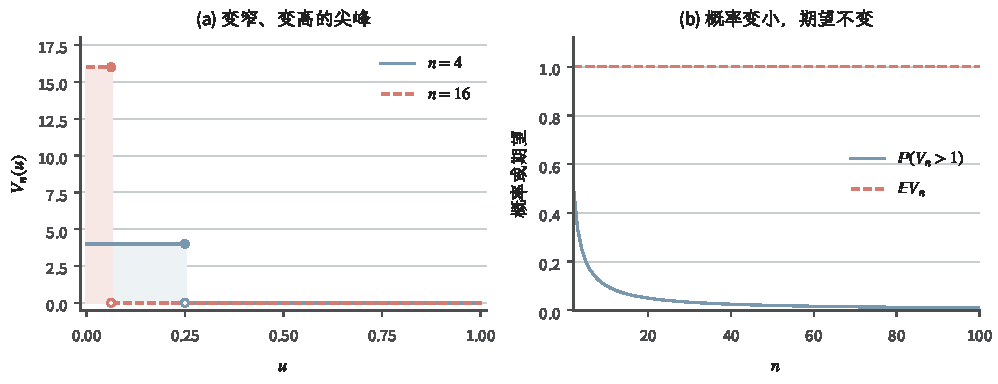
\includegraphics[width=\linewidth]{figures/math-preparation/concept-revision-probability/probability-vanishing-spikes.pdf}
  \caption{小概率尖峰与期望质量（解析式教学图）。左图为\(V_n(u)=n\mathbb I\{u\leq1/n\}\)在\(n=4,16\)时的取值，均以面积\(1\)贡献期望；右图对\(n\geq2\)显示\(\mathbb P(V_n>1)=1/n\)趋于零，而\(\mathbb E V_n=1\)不变。基础变量为\(U\sim\operatorname{Unif}(0,1)\)。}
  \label{fig:probability-vanishing-spikes}
\end{figure*}

\subsubsection{大数定律与样本平均}

\begin{theorem}[强大数定律]
\label{thm:probability-strong-law-large-numbers}
若\(X_1,X_2,\ldots\)独立同分布，且\(\mathbb{E}[|X_1|]<\infty\)，则
\[ \overline{X}_n
  =\frac{1}{n}\sum_{i=1}^{n}X_i\to_{\mathrm{a.s.}}\mathbb{E}[X_1]. \]
\end{theorem}

强大数定律说明同一分布下的独立重复观测，其平均几乎必然接近期望。有限方差是许多初等证明使用的方便条件，但独立同分布版本的结论只需有限一阶绝对矩。若观测相关、分布随
时间变化或样本由自适应规则收集，则不能直接引用该定理；第~\ref{chap:stochastic-processes-and-approximation}章将给出相关过程所需的替代条件
\scite{math-kallenberg2021probability}

有限方差时，较弱的依概率结论可以在这里完整得到。若
\(\operatorname{Var}(X_1)=\sigma^2<\infty\)，独立性使
\[
  \operatorname{Var}(\overline{X}_n)
  =\frac{1}{n^2}\sum_{i=1}^{n}\operatorname{Var}(X_i)
  =\frac{\sigma^2}{n}.
\]
把式~\eqref{eq:probability-chebyshev-inequality}用于样本平均，有
\[
  \mathbb{P}\bigl(
    |\overline{X}_n-\mathbb{E}X_1|\geq\varepsilon
  \bigr)
  \leq\frac{\sigma^2}{n\varepsilon^2}\to0.
\]
这证明了有限方差版本的弱大数定律。强大数定律只要求有限一阶绝对矩，但其证明还需截断大取值、控制截断变量的独立和，并把可求和坏事件转成几乎必然结论；不能由上面的逐个\(n\)概率界直接推出。

对例~\ref{ex:probability-noisy-observation}中的独立同分布噪声，只要\(\mathbb{E}|\varepsilon_i|<\infty\)，便有
\[ \overline{Y}_n
  =\theta+\frac{1}{n}\sum_{i=1}^{n}\varepsilon_i\to_{\mathrm{a.s.}}\theta. \]
这回答了“多测几次再平均是否稳定”，但没有给出固定\(n\)时误差超过指定阈值的概率。

\subsubsection{中心极限定理与缩放波动}

\begin{theorem}[Lindeberg--L\'evy中心极限定理]
\label{thm:probability-iid-central-limit}
若\(X_1,X_2,\ldots\)独立同分布，\(\mathbb{E}X_1=\mu\)，\(0<\operatorname{Var}(X_1)=\sigma^2<\infty\)，则
\[ \frac{\sqrt{n}(\overline{X}_n-\mu)}{\sigma}
  \Rightarrow\mathcal{N}(0,1). \]
\end{theorem}

大数定律研究未缩放误差是否趋于零，中心极限定理研究乘以\(\sqrt{n}\)后的剩余波动近似什么分布。它给出渐近近似，而不是每个有限\(n\)都精确服从高斯分布。若方差
无限、样本依赖过强或分布随\(n\)变化而不满足相应Lindeberg条件，\(\sqrt{n}\)缩放与高斯极限都可能失效。

证明的关键是特征函数。令\(Y_i=(X_i-\mu)/\sigma\)，并记
\(\varphi(t)=\mathbb{E}e^{\mathrm{i}tY_1}\)。复指数绝对值恒为\(1\)，所以特征函数总有定义。由
\(\mathbb{E}Y_1=0\)、\(\mathbb{E}Y_1^2=1\)及零点处的二阶展开，
\[
  \varphi(u)=1-\frac{u^2}{2}+o(u^2),
  \qquad u\to0.
\]
独立性使标准化和的特征函数分解为
\[
  \mathbb{E}\exp\left\{
    \mathrm{i}t\frac{1}{\sqrt n}\sum_{i=1}^{n}Y_i
  \right\}
  =
  \left[\varphi\left(\frac{t}{\sqrt n}\right)\right]^n
  \longrightarrow e^{-t^2/2}.
\]
右侧是标准高斯的特征函数，并且在零点连续。定理
~\ref{thm:probability-levy-continuity}于是给出依分布收敛。第
~\ref{chap:mathematical-statistics}章会用这个渐近分布构造近似区间，但有限样本覆盖
仍需额外误差控制，不能只引用极限式。

\subsection{蒙特卡洛平均与方差控制}
\label{sec:probability-monte-carlo-variance-reduction}

\subsubsection{直接蒙特卡洛估计}

目标积分可统一写成
\[ I=\mathbb{E}_P[f(X)]. \]
若能独立采样\(X_i\sim P\)，直接蒙特卡洛估计为
\[ \widehat{I}_n
  =\frac{1}{n}\sum_{i=1}^{n}f(X_i). \]
当\(\mathbb{E}_P|f(X)|<\infty\)时，大数定律给出一致性；当方差\(\sigma_f^2<\infty\)时，
\[ \operatorname{Var}(\widehat{I}_n)=\frac{\sigma_f^2}{n},
  \qquad\sqrt{n}(\widehat{I}_n-I)\Rightarrow\mathcal{N}(0,\sigma_f^2). \]
误差的标准差按\(n^{-1/2}\)下降，与输入维数没有显式关系，但
\(\sigma_f^2\)可能随问题结构急剧增大。

以下固定教学积分
\[ I=\int_0^1x^2\,\mathrm{d}x=\frac13. \]
若\(X\sim\operatorname{Unif}(0,1)\)，直接平均\(X_i^2\)的单样本方差为
\[ \operatorname{Var}(X^2)
  =\frac15-\frac19=\frac{4}{45}. \]

\subsubsection{重要性采样与方差}

若\(P\ll Q\)，权重\(w=\mathrm{d}P/\mathrm{d}Q\)，则
\[ I=\mathbb{E}_Q[w(X)f(X)]. \]
从\(Q\)采样得到无偏估计
\begin{equation}
  \widehat{I}^{\mathrm{IS}}_n
  =
  \frac{1}{n}\sum_{i=1}^{n}w(X_i)f(X_i),
  \qquad X_1,\ldots,X_n\text{独立同分布于 }Q.
  \label{eq:probability-importance-sampling}
\end{equation}
无偏性只要求乘积可积；有限方差还要求\(\mathbb{E}_Q[w^2f^2]<\infty\)。

对上述积分，取\(Q\)的密度\(q(x)=2x\)，而\(P\)为均匀分布。除零测点\(x=0\)外，\(w(x)=1/(2x)\)，于是\(w(x)f(x)=x/2\)。单样本方差变为
\[ \mathbb{E}_Q\left[\frac{X^2}{4}\right]-\frac19
  =\frac18-\frac19=\frac{1}{72}, \]
小于直接平均的\(4/45\)。这次改进来自\(Q\)把更多样本放到\(x^2\)贡献较大的区域。
并非任意改变分布都会降低方差；若\(Q\)在重要区域过轻，权重尾部反而会放大误差。

这个例子背后有一个理想基准。对固定的被积函数\(f\)，无偏改写其实不要求整个
\(P\ll Q\)，只要求\(Q\)支配有符号测度\(f\,\mathrm{d}P\)：若\(Q(A)=0\)，则
\(\int_A|f|\,\mathrm{d}P=0\)。当\(P,Q\)相对于同一测度分别有密度\(p,q\)时，这等价于
\(q(x)>0\)在\(|f(x)|p(x)>0\)处几乎处处成立。此时令
\[
  h_Q(x)=\frac{f(x)p(x)}{q(x)},\qquad q(x)>0,
\]
便有\(I=\mathbb{E}_Q[h_Q(X)]\)。若
\(0<\mathbb{E}_P|f(X)|<\infty\)，则在满足这一支配条件的提议密度中，使
\(\mathbb{E}_Q[h_Q^2]\)最小的选择满足
\[
  q^\star(x)
  =
  \frac{|f(x)|p(x)}{\mathbb{E}_P|f(X)|}.
\]
它把采样质量直接放到被积函数绝对贡献大的区域。若\(f(x)=0\)而\(p(x)>0\)，则
\(q^\star(x)=0\)，所以一般并没有\(P\ll Q^\star\)，密度比\(p/q^\star\)也不必在该点
定义；但该点对\(f\,\mathrm{d}P\)没有贡献，而且不会被\(Q^\star\)采到，只需把
\(h_{Q^\star}\)定义到\(Q^\star\)-几乎处处即可。特别地，当\(f\geq0\)时，
\(q^\star=fp/I\)，且\(h_{Q^\star}(X)=I\)在\(Q^\star\)下几乎处处成立，理论方差为零。

这个分布通常不能直接执行：归一化常数就是未知积分\(I\)，而从\(fp/I\)精确采样也可能
与原问题一样困难。若还要用同一组权重估计其他被积函数，因而必须保留\(P\ll Q\)，可以
取\(q_\eta=(1-\eta)q^\star+\eta p\)，其中\(0<\eta<1\)；混入的\(p\)为所有
\(P\)-正质量区域保留严格正支持。理想分布因此只提供设计直觉；实际提议分布还必须能够
归一化、采样并计算密度，同时覆盖\(|f|p\)非零的区域。

\subsubsection{控制变量与相关性}

若辅助变量\(h(X)\)的均值\(\mu_h\)已知，则对任意\(\beta\)，
\[ f_\beta(X)
  =f(X)-\beta(h(X)-\mu_h) \]
仍有期望\(I\)。其方差为
\[ \operatorname{Var}(f_\beta)
  =\operatorname{Var}(f)-2\beta\operatorname{Cov}(f,h)+\beta^2\operatorname{Var}(h). \]
当\(\operatorname{Var}(h)>0\)时，最优系数为
\[ \beta^\star
  =\frac{\operatorname{Cov}(f,h)}{\operatorname{Var}(h)}. \]
对\(f(X)=X^2\)、\(h(X)=X\)与均匀\(X\)，有
\(\mu_h=1/2\)且\(\beta^\star=1\)。调整后的变量
\[ X^2-X+\frac12 \]
仍以\(1/3\)为均值，方差降为\(1/180\)。实际用同一批数据估计\(\beta^\star\)时，有限样本无偏性和方差公式需要重新核对；把估计系数当成固定常数会忽略额外随机性。

\subsubsection{Rao--Blackwell化与方差分解}

设\(Y\)是目标\(I\)的无偏估计，\(\mathbb{E}[Y^2]<\infty\)。对某个统计量\(T\)定义
\[ Y^\star=\mathbb{E}[Y\mid T]. \]
全期望公式给出\(\mathbb{E}Y^\star=I\)，全方差公式给出
\begin{equation}
  \operatorname{Var}(Y)
  =
  \mathbb{E}[\operatorname{Var}(Y\mid T)]
  +
  \operatorname{Var}(Y^\star)
  \geq
  \operatorname{Var}(Y^\star).
  \label{eq:probability-rao-blackwell-variance}
\end{equation}
这就是Rao--Blackwell化：在保持均值的同时，对已知信息求条件平均，消去条件内噪声。

仍以\(I=1/3\)为例。独立生成\(X,U\sim\operatorname{Unif}(0,1)\)，令
\[ Y=\mathbb{I}\{U\leq X^2\}. \]
则\(\mathbb{E}Y=1/3\)，而\(\mathbb{E}[Y\mid X]=X^2\)。因此直接平均\(X^2\)可以看成命中估计\(Y\)关于\(X\)的Rao--Blackwell化，方差从
\((1/3)(2/3)=2/9\)降为\(4/45\)。

\subsubsection{自归一化权重与比值估计}

设\(P\ll Q\)，但只能在未知公共常数倍的意义下计算目标密度比，即对某个\(c>0\)，
\[
  \widetilde{w}(x)
  =
  c\,\frac{\mathrm{d}P}{\mathrm{d}Q}(x),
\]
在\(Q\)-几乎处处意义下成立。对独立同分布样本\(X_i\sim Q\)，在分母为正时使用
\(\widetilde{w}_i=\widetilde{w}(X_i)\)并定义
\begin{equation}
  \widehat{I}^{\mathrm{SN}}_n
  =
  \frac{\sum_{i=1}^{n}\widetilde{w}_if(X_i)}
       {\sum_{i=1}^{n}\widetilde{w}_i}.
  \label{eq:probability-self-normalized-importance-sampling}
\end{equation}
它是两个随机平均的比值，通常在有限样本下有偏，因为一般而言\(\mathbb{E}[A/B]\neq\mathbb{E}A/\mathbb{E}B\)。在适当矩条件和分母极限为正时，大数定律仍可给出一致性。
更具体地，若
\(\mathbb{E}_Q[|\widetilde{w}f|]<\infty\)且
\(0<\mathbb{E}_Q[\widetilde{w}]<\infty\)，则强大数定律给出
\[
  \widehat{I}^{\mathrm{SN}}_n
  \longrightarrow
  \frac{\mathbb{E}_Q[\widetilde{w}f]}
       {\mathbb{E}_Q[\widetilde{w}]}
  =
  \frac{c\mathbb{E}_P[f]}{c}
  =I
  \qquad\text{几乎必然}.
\]
若\(\widetilde{w}\)不是目标密度比的公共常数倍，同一比值仍可能收敛，但极限一般对应另一个归一化加权分布，不能据此声称估计的是
\(\mathbb{E}_P[f]\)。

一个三点分布可以同时看清方差、截断与重采样的不同作用。令支持集为
\(\{a,b,c\}\)，提议分布和目标分布分别为
\[
  Q=(0.8,0.15,0.05),\qquad
  P=(0.4,0.3,0.3),
\]
于是重要性权重为\(w=(0.5,2,6)\)。对
\(f=(0,1,1)\)，目标均值为\(I=0.6\)。原始单样本贡献
\(Z=wf=(0,2,6)\)满足
\[
  \mathbb{E}_Q Z=0.6,\qquad
  \operatorname{Var}_Q(Z)
  =\{0.15\times4+0.05\times36\}-0.6^2
  =2.04.
\]
因此\(n\)个独立样本的无偏估计方差为\(2.04/n\)。若把权重截断在\(2\)，则
\(w^{(2)}=(0.5,2,2)\)，相应贡献的期望变为\(0.4\)，方差变为
\[
  \{0.15\times4+0.05\times4\}-0.4^2=0.64.
\]
截断降低了方差，却引入\(-0.2\)的偏差；两者必须同时报告。

再看一组恰好含\(16\)个\(a\)、\(3\)个\(b\)和\(1\)个\(c\)的二十粒子样本。
原始权重总和为\(20\)，归一化后的三点质量恰为\((0.4,0.3,0.3)\)。按这些质量做
\(20\)次多项重采样，三点后代数的条件期望为\((8,6,6)\)；重采样后无权平均的条件
期望仍为\(0.6\)，但条件方差增加了
\[
  \frac{0.6(1-0.6)}{20}=0.012.
\]
若先截断，归一化质量变成\((0.5,0.375,0.125)\)，重采样均值的条件期望是\(0.5\)，
不会恢复被截断改变的目标。原始和截断权重在这组粒子上的经验有效样本量分别约为
\(400/52=7.69\)与\(256/20=12.8\)：较均匀的权重提高了这一诊断量，但不证明偏差消失。

经验有效样本量常写成
\[ \widehat{n}_{\mathrm{eff}}
  =\frac{(\sum_i\widetilde{w}_i)^2}{\sum_i\widetilde{w}_i^2}. \]
它是权重退化的诊断量，不是对所有估计目标都成立的精确独立样本数。截断权重可降低
方差，却通常引入偏差；重采样减少后续计算中的权重不均，却增加额外随机性。本节的“自归一化”是随机比值估计，第~\ref{sec:stoch-self-normalized-adaptive-design}节的自归一化集中则用随机设计矩阵度量累计噪声，二者对象不同。

\subsection{尾部概率与集中不等式}
\label{sec:probability-concentration-inequalities}

\subsubsection{Chernoff方法与指数矩}

对任意\(\lambda>0\)，函数\(x\mapsto e^{\lambda x}\)单调。Markov不等式给出
\begin{equation}
  \mathbb{P}(X\geq t)
  =
  \mathbb{P}(e^{\lambda X}\geq e^{\lambda t})
  \leq
  e^{-\lambda t}\mathbb{E}[e^{\lambda X}].
  \label{eq:probability-chernoff-step}
\end{equation}
随后对\(\lambda\)优化，便得到Chernoff方法。整个方法依赖相应指数矩有限；若\(\mathbb{E}e^{\lambda X}=\infty\)，式
\eqref{eq:probability-chernoff-step}虽形式上仍真，却不给出有用上界。

\begin{definition}[次高斯变量]
  \label{def:probability-subgaussian}
对\(\sigma^2>0\)，均值为零的可积实随机变量\(X\)若满足
\[ \mathbb{E}[e^{\lambda X}]
  \leq\exp\left(\frac{\lambda^2\sigma^2}{2}\right),\qquad \lambda\in\mathbb{R}, \]
就称它为参数\(\sigma^2\)的\term{次高斯变量}（sub-Gaussian random variable）。
\end{definition}
代入Chernoff界并取\(\lambda=t/\sigma^2\)，得到
\[ \mathbb{P}(X\geq t)
  \leq\exp\left(-\frac{t^2}{2\sigma^2}\right). \]
“次高斯”描述的是指数矩或尾部上界，不表示变量本身服从高斯分布。

\subsubsection{有界变量的Hoeffding不等式}

\begin{lemma}[Hoeffding引理]
\label{lem:probability-hoeffding-lemma}
若\(\mathbb{E}X=0\)且\(X\in[a,b]\)几乎处处成立，则
\[ \mathbb{E}[e^{\lambda X}]
  \leq\exp\left\{\frac{\lambda^2(b-a)^2}{8}\right\},\qquad \lambda\in\mathbb{R}. \]
\end{lemma}

\begin{proof}
凸性说明，对\(x\in[a,b]\)，指数函数位于连接端点的弦下方：
\[ e^{\lambda x}
  \leq\frac{b-x}{b-a}e^{\lambda a}+\frac{x-a}{b-a}e^{\lambda b}. \]
取期望并使用\(\mathbb{E}X=0\)，右侧成为一个只依赖
\(\lambda(b-a)\)与均值位置的二点分布矩母函数。令\(p=-a/(b-a)\)，对其对数作二阶导数，可得二阶导数至多为\(1/4\)；该对数在
\(\lambda=0\)处的函数值和一阶导数均为零。两次积分于是给出
\[ \log\mathbb{E}[e^{\lambda X}]
  \leq\frac{\lambda^2(b-a)^2}{8}. \]
指数化即得结论。
\end{proof}

\begin{theorem}[Hoeffding不等式]
\label{thm:probability-hoeffding-inequality}
设\(X_1,\ldots,X_n\)相互独立，且\(X_i\in[a_i,b_i]\)几乎处处成立。则对\(t>0\)，
\[
  \mathbb{P}\left(
    \sum_{i=1}^{n}(X_i-\mathbb{E}X_i)\geq t
  \right)
  \leq
  \exp\left\{
    -\frac{2t^2}{\sum_{i=1}^{n}(b_i-a_i)^2}
  \right\}.
\]
\end{theorem}

\begin{proof}
记\(S=\sum_i(X_i-\mathbb{E}X_i)\)。对\(\lambda>0\)，独立性使指数矩分解：
\[
\begin{aligned}
  \mathbb{P}(S\geq t)
  &\leq
  e^{-\lambda t}\mathbb{E}[e^{\lambda S}]\\
  &=
  e^{-\lambda t}
  \prod_{i=1}^{n}
  \mathbb{E}\left[
    e^{\lambda(X_i-\mathbb{E}X_i)}
  \right]\\
  &\leq
  \exp\left\{
    -\lambda t+
    \frac{\lambda^2}{8}
    \sum_{i=1}^{n}(b_i-a_i)^2
  \right\}.
\end{aligned}
\]
右侧关于\(\lambda\)的最小点为
\[ \lambda^\star
  =\frac{4t}{\sum_i(b_i-a_i)^2}. \]
代回即得结论。对\(-S\)使用同一结果，再用联合界可得双侧版本。
\end{proof}

若\(X_i\in[0,1]\)独立，则样本平均满足
\[ \mathbb{P}(|\overline{X}_n-\mathbb{E}\overline{X}_n|
  \geq\varepsilon)\leq 2e^{-2n\varepsilon^2}. \]
有界性进入Hoeffding引理，独立性进入矩母函数乘积；删除任一条件都不能沿用这份证明。

\subsubsection{方差敏感的Bernstein不等式}

若独立中心化变量满足\(|X_i|\leq M\)，并记\(v=\sum_i\mathbb{E}[X_i^2]\)，则Bernstein不等式的一个版本为
\begin{equation}
  \mathbb{P}\left(\sum_{i=1}^{n}X_i\geq t\right)
  \leq
  \exp\left\{
    -\frac{t^2}{2(v+Mt/3)}
  \right\}.
  \label{eq:probability-bernstein-inequality}
\end{equation}
为看清两个尺度的来源，取\(0<\lambda<3/M\)。由指数级数及
\(|X_i|^k\leq M^{k-2}X_i^2\)（\(k\geq2\)），有
\[
  \mathbb{E}e^{\lambda X_i}
  \leq
  1+\frac{\lambda^2\mathbb{E}X_i^2}
           {2(1-\lambda M/3)}
  \leq
  \exp\left\{
    \frac{\lambda^2\mathbb{E}X_i^2}
         {2(1-\lambda M/3)}
  \right\}.
\]
这里第一阶项因中心化而消失，常数\(1/3\)来自用几何级数控制
\[
  \sum_{k\geq3}\frac{(\lambda M)^{k-2}}{k!}.
\]
独立性使各指数矩相乘，Chernoff步骤于是给出
\[
  \mathbb{P}\left(\sum_iX_i\geq t\right)
  \leq
  \exp\left\{
    -\lambda t+\frac{\lambda^2v}
      {2(1-\lambda M/3)}
  \right\}.
\]
取\(\lambda=t/(v+Mt/3)\)便得到式~\eqref{eq:probability-bernstein-inequality}。小偏差区域由\(v\)主导，呈高斯型；大偏差区域由\(Mt\)主导，呈指数型。

例如\(B_i\sim\operatorname{Bernoulli}(0.01)\)独立，考虑
\(\overline{B}_n-0.01\geq0.05\)。Hoeffding上界为
\(\exp(-0.005n)\)，而Bernstein上界约为
\[
  \exp\left\{
    -\frac{0.05^2n}
      {2(0.01\times0.99+0.05/3)}
  \right\}
  \approx \exp(-0.047n).
\]
低发生率使实际方差远小于区间最坏尺度，所以后者明显更紧；当方差接近区间允许的最大值或偏差进入线性尺度时，Bernstein并不保证处处优于Hoeffding。

对重尾变量，方差可能不存在，指数矩也可能对所有正参数发散。此时Chebyshev、Hoeffding和Bernstein各自在矩、范围或指数矩步骤失效。可以增加截断、稳健均值或仅用
有限\(p\)阶矩推导多项式尾界，但所得估计对象和偏差需要重新说明，不能继续声称高斯型集中。

\section{同时控制与重排对称}
\label{sec:probability-uniform-errors-symmetry}

上节主要控制一个预先指定的平均。按数据选择候选时，需要让误差界对所有可能被选中的对象同时成立，
这引出函数类的联合误差。章末再考察另一种保证来源：如果观测重排后联合分布不变，
即使没有独立性，秩也可能给出精确的有限样本覆盖。两条路线依赖不同条件。

\subsection{多个对象与随机函数的联合误差}
\label{sec:probability-random-functions-uniform-error}

\subsubsection{有限候选的一致误差}

设有限候选类\(\mathcal{H}=\{h_1,\ldots,h_M\}\)，损失\(\ell(h,Z)\in[0,1]\)。真实风险与经验风险分别为
\[ R(h)=\mathbb{E}[\ell(h,Z)],
  \qquad\widehat{R}_n(h)=\frac{1}{n}\sum_{i=1}^{n}\ell(h,Z_i), \]
其中\(Z_1,\ldots,Z_n\)独立同分布。对预先固定的单个\(h\)，Hoeffding不等式给出
\[ \mathbb{P}\bigl(
    |\widehat{R}_n(h)-R(h)|>\varepsilon\bigr)\leq 2e^{-2n\varepsilon^2}. \]
但经验最优候选
\(\widehat{h}\in\arg\min_h\widehat{R}_n(h)\)由同一批数据选出，不是预先固定对象。只控制一个候选不能排除“恰好因噪声看起来最好”的选择偏差。

为明确“同时控制”与“样本量足够”的关系，把上述要求写成一个定义。这里讨论抽样前固定的函数类；所有上确界均假定可测。一项常用充分条件是存在可数子类，使每个函数都是该子类中某个序列的逐点极限。
\begin{definition}[分布无关的一致收敛]
  \label{def:uniform-convergence}
  设\(\mathcal G\)是非空的\([0,1]\)值可测函数类。若对任意\(\eta,\delta\in(0,1)\)，存在只依赖\(\mathcal G,\eta,\delta\)的整数\(n_0\)，使任意概率分布\(P\)和任意\(n\geq n_0\)的独立同分布样本\(S=(Z_1,\ldots,Z_n)\sim P^n\)均满足
  \begin{equation}
    \mathbb P_{S\sim P^n}\left\{
      \sup_{g\in\mathcal G}\left|\frac1n\sum_{i=1}^ng(Z_i)-\mathbb E_Pg\right|\leq\eta
    \right\}\geq1-\delta,
    \label{eq:uniform-convergence-definition}
  \end{equation}
  就称\(\mathcal G\)满足分布无关的\term{一致收敛}（uniform convergence）。若只要求\(P\)属于指定分布族，同一定义给出相对于该分布族的一致收敛。
\end{definition}
“函数上一致”由上确界表达，“分布无关”则要求同一个\(n_0\)适用于全部允许分布。对每个固定函数或每个固定分布分别存在的样本量，不能自动满足这两个量词。

\begin{theorem}[有限函数类的一致误差界]
\label{thm:probability-finite-class-uniform-bound}
在上述条件下，对任意\(\delta\in(0,1)\)，以至少\(1-\delta\)的概率同时对所有\(h\in\mathcal{H}\)有
\begin{equation}
  |\widehat{R}_n(h)-R(h)|
  \leq
  \sqrt{\frac{\log(2M/\delta)}{2n}}.
  \label{eq:probability-finite-class-bound}
\end{equation}
\end{theorem}

\begin{proof}
对每个\(h\)定义坏事件
\[ A_h=
  \{|\widehat{R}_n(h)-R(h)|>\varepsilon\}. \]
单函数Hoeffding界给出\(\mathbb{P}(A_h)\leq2e^{-2n\varepsilon^2}\)。由联合界，
\[ \mathbb{P}\left(\bigcup_{h\in\mathcal{H}}A_h\right)
  \leq 2M e^{-2n\varepsilon^2}. \]
令右侧等于\(\delta\)，解得\(\varepsilon=\sqrt{\log(2M/\delta)/(2n)}\)。在坏事件并集的补集上，结论对
全部候选同时成立。
\end{proof}

令\(h^\star\in\arg\min_hR(h)\)，并在式\eqref{eq:probability-finite-class-bound}成立的事件上记右侧为\(\varepsilon_n\)。则
\[
\begin{aligned}
  R(\widehat{h})
  &\leq
  \widehat{R}_n(\widehat{h})+\varepsilon_n\\
  &\leq
  \widehat{R}_n(h^\star)+\varepsilon_n\\
  &\leq
  R(h^\star)+2\varepsilon_n.
\end{aligned}
\]
第二步正是经验最优性的用途。候选数只通过\(\log M\)进入，但若候选类本身由同一数据任意生成，简单地把最终数量代入\(M\)未必合法；需要把生成过程纳入统一控制对象。
例如\(M=100\)、\(n=1000\)、\(\delta=0.05\)时，式~\eqref{eq:probability-finite-class-bound}右侧约为
\[
  \sqrt{\frac{\log 4000}{2000}}\approx0.0644.
\]
这个数同时控制一百个预先固定候选，而不是给每个候选各自提供\(95\%\)保证；后一做法的联合失败概率可能远大于\(5\%\)。

\subsubsection{覆盖数与随机投影}

无限函数类不能直接按元素做联合界。第~\ref{chap:functional-analysis-and-approximation}章建立的取值模式与覆盖数提供两种
有限化方法：若样本上只有有限种损失向量，只需对这些模式联合控制；若每个函数都能由有限\(\varepsilon\)-网中的代表逼近，则先控制网点，再用Lipschitz性质把误差转回
原函数。这里的关键不是形式上把“无限”改写成一个大数字，而是证明离散代表确实控制所需误差度量。

\begin{lemma}[覆盖数的有限网控制]
  \label{lem:probability-covering-finite-net}
  设\((\mathcal{F},d)\)具有有限\(\varepsilon\)-网
  \(\mathcal{N}_\varepsilon\)，其大小为
  \(N(\mathcal{F},d,\varepsilon)\)。若随机过程
  \(\{Z_f:f\in\mathcal{F}\}\)满足
  \[
    |Z_f-Z_g|\leq Ld(f,g)
  \]
  几乎处处对所有\(f,g\)成立，并且相关上确界可测，则对任意\(t>0\)，
  \begin{equation}
    \mathbb{P}\left\{
      \sup_{f\in\mathcal{F}}|Z_f|>t+L\varepsilon
    \right\}
    \leq
    N(\mathcal{F},d,\varepsilon)
    \sup_{f\in\mathcal{F}}\mathbb{P}(|Z_f|>t).
    \label{eq:probability-covering-finite-net}
  \end{equation}
\end{lemma}

\begin{proof}
对每个\(f\)选取满足\(d(f,g_f)\leq\varepsilon\)的
\(g_f\in\mathcal{N}_\varepsilon\)。则
\[
  |Z_f|\leq |Z_{g_f}|+L\varepsilon,
\]
所以左侧坏事件包含在
\(\bigcup_{g\in\mathcal{N}_\varepsilon}\{|Z_g|>t\}\)中。对这个有限并集使用联合界
即得结论。
\end{proof}

若\(Z_f=\widehat R_n(f)-R(f)\)，且经验风险与真实风险各自关于\(d\)都是
\(L_0\)-Lipschitz，则引理中的过程常数是\(2L_0\)。因此，网格大小、离散误差
\(2L_0\varepsilon\)和单点尾界必须一起进入结论；只报告覆盖数而不验证Lipschitz传递
还不能控制原函数类。

下面的随机投影会把范数失真化成高斯平方和。
\begin{definition}[卡方分布]
  \label{def:probability-chi-square-distribution}
若\(G_1,\ldots,G_k\)相互独立且都服从标准高斯分布\(\mathcal N(0,1)\)，则称
\[
  Z=\sum_{j=1}^{k}G_j^2
\]
服从自由度为\(k\)的\term{卡方分布}（chi-square distribution），记为
\(Z\sim\chi_k^2\)，其中\(k\)为正整数。
\end{definition}
这个定义也给出后文调用尾界的接口：只要证明一个随机二次量能写成
\(k\)个独立标准高斯的平方和，就可以直接使用下面的结论。

\begin{lemma}[\(\chi^2\)变量的尾界]
  \label{lem:probability-chi-square-tail}
  若\(Z\sim\chi_k^2\)，其中\(k\)为正整数，则对每个\(x>0\)，
  \[
    \mathbb{P}\{Z-k\geq2\sqrt{kx}+2x\}\leq e^{-x},
    \qquad
    \mathbb{P}\{k-Z\geq2\sqrt{kx}\}\leq e^{-x}.
  \]
  因而对\(0<\varepsilon<1\)，
  \begin{equation}
    \mathbb{P}\left(
      \left|\frac{Z}{k}-1\right|>\varepsilon
    \right)
    \leq2\exp\left(-\frac{k\varepsilon^2}{8}\right).
    \label{eq:probability-chi-square-relative-tail}
  \end{equation}
\end{lemma}

\begin{proof}
标准高斯积分给出\(\mathbb E e^{\lambda G^2}=(1-2\lambda)^{-1/2}\)，\(\lambda<1/2\)。独立性因而给出
\[
  \log\mathbb E e^{\lambda(Z-k)}
  =\frac{k}{2}\{-2\lambda-\log(1-2\lambda)\}
  \leq\frac{k\lambda^2}{1-2\lambda},\qquad 0<\lambda<1/2.
\]
最后一步来自\(-u-\log(1-u)=\sum_{j\geq2}u^j/j\leq u^2/[2(1-u)]\)。对上尾使用Chernoff方法，取
\(\lambda=\sqrt{x}/(\sqrt{k}+2\sqrt{x})\)，便在阈值\(2\sqrt{kx}+2x\)处得到指数\(-x\)。
对下尾，用\(u-\log(1+u)\leq u^2/2\)得到
\[
  \log\mathbb E e^{-\lambda(Z-k)}\leq k\lambda^2,\qquad\lambda>0.
\]
取\(\lambda=\sqrt{x/k}\)，在阈值\(2\sqrt{kx}\)处也得到指数\(-x\)。最后取\(x=k\varepsilon^2/8\)。当\(0<\varepsilon<1\)时，两侧阈值均不超过\(k\varepsilon\)，故相对偏差事件包含于对应尾事件的并集，联合界给出式~\eqref{eq:probability-chi-square-relative-tail}。
\end{proof}

现在把单个方向的集中推广到有限点集。这一结果称为Johnson--Lindenstrauss引理：保留有限个距离所需的随机投影维数主要随点数的对数增长，而不由原始坐标数直接决定。
\begin{theorem}[高斯随机投影的距离保持]
  \label{thm:probability-johnson-lindenstrauss}
  给定抽样前固定的\(N\geq2\)个点\(\bm x_1,\ldots,\bm x_N\in\mathbb R^d\)，以及\(\varepsilon,\delta\in(0,1)\)。若\(\bm A\in\mathbb R^{k\times d}\)的元素独立服从\(\mathcal N(0,1/k)\)，且
  \[
    k\geq\frac8{\varepsilon^2}\log\frac{N(N-1)}\delta,
  \]
  则以至少\(1-\delta\)的概率，对全部\(i,j\)同时有
  \begin{equation}
    (1-\varepsilon)\|\bm x_i-\bm x_j\|_2^2
    \leq\|\bm A\bm x_i-\bm A\bm x_j\|_2^2
    \leq(1+\varepsilon)\|\bm x_i-\bm x_j\|_2^2.
    \label{eq:probability-jl-distance-preservation}
  \end{equation}
\end{theorem}
\begin{proof}
固定一个不依赖\(\bm A\)的非零向量\(\bm v\)。矩阵各行独立，每个\((\bm A\bm v)_r\)均为均值零、方差\(\|\bm v\|_2^2/k\)的高斯变量，因此
\[
  \frac{k\|\bm A\bm v\|_2^2}{\|\bm v\|_2^2}\sim\chi_k^2.
\]
引理~\ref{lem:probability-chi-square-tail}使该方向的相对平方范数失真概率不超过\(2e^{-k\varepsilon^2/8}\)。点对差至多有\(N(N-1)/2\)个；对全部非零差使用联合界，失败概率不超过\(N(N-1)e^{-k\varepsilon^2/8}\leq\delta\)。零差经任何线性投影仍为零，无须额外尾界。
\end{proof}
结论控制的是平方距离；对距离本身开方后，因子为\(\sqrt{1\pm\varepsilon}\)。点集须在投影抽样前确定，但在同时保持事件上，可以事后任选这批点中的一对查询。它不保证对观察到\(\bm A\)后任意新造的向量都保持范数；当\(k<d\)时，\(\bm A\)的非零零空间方向就给出反例。这里的常数是便于推导的充分界，也不保证所得\(k\)一定小于\(d\)。

\subsubsection{有界差与数据函数集中}

有些目标不是单个样本平均，而是整个数据集的函数\(F(Z_1,\ldots,Z_n)\)。若替换第\(i\)个输入最多改变\(c_i\)，即
\[ \sup_{\bm{z},z_i'}
  |F(z_1,\ldots,z_i,\ldots,z_n)-F(z_1,\ldots,z_i',\ldots,z_n)|\leq c_i, \]
则独立输入下的McDiarmid不等式给出
\begin{equation}
  \mathbb{P}\bigl(
    F-\mathbb{E}F\geq t
  \bigr)
  \leq
  \exp\left\{
    -\frac{2t^2}{\sum_{i=1}^{n}c_i^2}
  \right\}.
  \label{eq:probability-mcdiarmid}
\end{equation}
其证明把\(F\)依次对前\(i\)个观测条件化，形成Doob鞅；每步有界差控制一个鞅增量，再使用Hoeffding型指数矩界。独立性保证逐步揭示观测时的条件结构，有界差则限制单个观测的影响。

\subsubsection{经验复杂度与随机系数}

有限候选可按数量控制误差；无限类的函数在同一组观测上可能高度相似，直接计数会忽略这种结构。\term{Rademacher复杂度}提供另一种衡量方式：固定观测点后，让函数尽量对齐一组无信号的随机正负号，再对这些正负号平均。能拟合更多随机起伏的类，需要更大的同时误差代价。
\begin{definition}[经验Rademacher复杂度]
  \label{def:rademacher-complexity}
  给定非空实值可测函数类\(\mathcal G\)和样本\(S=(z_1,\ldots,z_n)\)。令\(\sigma_i\)独立且等概率取\(-1,1\)。当上确界可测且期望有限时，\term{经验Rademacher复杂度}定义为
  \begin{equation}
    \widehat{\mathfrak R}_S(\mathcal G)
    =\mathbb E_\sigma\left[\sup_{g\in\mathcal G}\frac1n\sum_{i=1}^n\sigma_i g(z_i)\right].
    \label{eq:empirical-rademacher}
  \end{equation}
\end{definition}
固定的是样本，不是使随机和最大的函数；每一组符号都允许选择不同函数。交换上确界与期望会把所有固定函数的零均值随机和平均成零，丢掉所要衡量的拟合能力。
\begin{definition}[期望Rademacher复杂度]
  \label{def:expected-rademacher-complexity}
  对\(S\sim P^n\)，\term{期望Rademacher复杂度}定义为
  \[
    \mathfrak R_n(\mathcal G)=\mathbb E_{S\sim P^n}\widehat{\mathfrak R}_S(\mathcal G).
  \]
\end{definition}
期望复杂度还平均了抽样结果，故依赖\(P\)；经验复杂度仅依赖给定样本上的函数取值。
允许函数作凸组合会增加候选函数，却未必增加它们对随机符号的最大对齐能力。
原因在于，固定符号后，经验随机和是函数取值的线性泛函：若一个组合的各项都不超过
同一个上界，非负且归一化的加权平均也不能超过它。下面把这一几何性质写成复杂度恒等式。

\begin{theorem}[凸组合的Rademacher复杂度]
\label{thm:ensemble-convex-hull}
设$S=(z_1,\ldots,z_n)$为固定样本，$n\geq1$，$\mathcal B$为非空实值可测函数类，
且在这组样本上统一有界，即存在有限$M$使$|h(z_i)|\leq M$对所有
$h\in\mathcal B$和$i$成立。令
\[
 \operatorname{conv}(\mathcal B)
 =\left\{\sum_{t=1}^T a_t h_t:
 T\geq1,\ h_t\in\mathcal B,\ a_t\geq0,\ \sum_{t=1}^T a_t=1\right\}
\]
为全部有限凸组合构成的函数类。则
\[
 \widehat{\mathfrak R}_S(\operatorname{conv}(\mathcal B))
 =\widehat{\mathfrak R}_S(\mathcal B).
\]
若样本再按$P^n$抽取，几乎必然满足上述样本有界条件，且相应样本上确界可测、期望有限，
则期望Rademacher复杂度也满足同一恒等式。
\end{theorem}

\begin{proof}
固定一组符号$\bm\sigma$。对任意有限凸组合，由$a_t\geq0$和$\sum_ta_t=1$，
\[
 \begin{aligned}
 \frac1n\sum_{i=1}^n\sigma_i\sum_{t=1}^T a_t h_t(z_i)
 &=\sum_{t=1}^T a_t
    \left(\frac1n\sum_{i=1}^n\sigma_i h_t(z_i)\right)\\
 &\leq\sup_{h\in\mathcal B}\frac1n\sum_{i=1}^n\sigma_i h(z_i).
 \end{aligned}
\]
因此凸包上的上确界不超过基类上的上确界。反向不等式来自
$\mathcal B\subseteq\operatorname{conv}(\mathcal B)$：取$T=1$即可得到任意基函数。
于是每一组符号下的两个上确界都相等。样本上的统一有界性保证随机和与其上确界有限，
对$\bm\sigma$取期望便得经验复杂度恒等式；在额外的抽样可测性与可积条件下，再对$S$
取期望即得期望复杂度结论。证明不要求函数类有限，也不要求上确界由某个函数达到。
\end{proof}

例如，只含常值函数$0$和$1$的基类，其凸包包含全部常值$c\in[0,1]$。
固定一个观测点时，正号下的最大随机和为$1$，负号下为$0$，两类的经验复杂度都为
$1/2$。候选函数从两个增加到无穷多个，但线性随机和的最坏值仍由端点决定。
这一定理只控制实值函数的随机线性和；把组合再作阈值化等非线性变换后，
需要另外分析变换后的函数类。非负性与归一化也是凸组合的条件，不能用同一等式处理
任意符号或任意尺度的线性组合。

\begin{definition}[经验高斯复杂度]
  \label{def:gaussian-complexity}
  将随机符号换成独立标准高斯系数\(\xi_i\sim\mathcal N(0,1)\)，定义
  \[
    \widehat{\mathfrak G}_S(\mathcal G)
    =\mathbb E_\xi\left[\sup_{g\in\mathcal G}\frac1n\sum_{i=1}^n\xi_i g(z_i)\right].
  \]
  相应期望高斯复杂度为\(\mathfrak G_n(\mathcal G)=\mathbb E_S\widehat{\mathfrak G}_S(\mathcal G)\)。
\end{definition}
高斯系数的符号与幅度都变化，Rademacher系数只有符号变化。二者是关于函数类的随机平均，不能按某一组系数的最大值直接比较。

双侧误差的证明常使用带绝对值版本
\[
  \widehat{\mathfrak R}^{\mathrm{abs}}_S(\mathcal G)
  =\mathbb E_\sigma\sup_{g\in\mathcal G}\left|\frac1n\sum_i\sigma_i g(z_i)\right|
  =\widehat{\mathfrak R}_S(\mathcal G\cup(-\mathcal G)),
\]
高斯版本同样定义。只有当\(\mathcal G=-\mathcal G\)时，两种约定才可直接等同。例如只含常数函数\(g\equiv1\)的类，其不带绝对值复杂度为\(0\)；带绝对值复杂度为\(n^{-1}\mathbb E|\sum_i\sigma_i|>0\)。以下对称化沿用带绝对值约定，后续应用单侧风险界时应核对所用版本。

\subsubsection{对称化与随机函数复杂度}

设\(\mathcal{F}\)是一族取值于\([-1,1]\)的函数，定义
\[ \Delta(\bm{Z})
  =\sup_{f\in\mathcal{F}}\left|\mathbb{E}f(Z)-\frac{1}{n}\sum_{i=1}^{n}f(Z_i)\right|. \]
引入独立同分布副本\(Z_1',\ldots,Z_n'\)。Jensen不等式给出
\[
\begin{aligned}
  \mathbb{E}_{\bm{Z}}\Delta(\bm{Z})
  &\leq
  \mathbb{E}_{\bm{Z},\bm{Z}'}
  \sup_{f\in\mathcal{F}}
  \left|
    \frac{1}{n}\sum_{i=1}^{n}
    \bigl(f(Z_i')-f(Z_i)\bigr)
  \right|.
\end{aligned}
\]
由于每对\((Z_i,Z_i')\)交换后联合分布不变，引入独立Rademacher符号\(\sigma_i\in\{-1,1\}\)不会改变差的联合分布。因此
\[
  \mathbb{E}\Delta(\bm{Z})
  \leq
  2\mathbb{E}_{\bm{Z},\bm{\sigma}}
  \sup_{f\in\mathcal{F}}
  \left|
    \frac{1}{n}\sum_{i=1}^{n}\sigma_i f(Z_i)
  \right|.
\]
右侧是带绝对值的经验Rademacher复杂度对样本取期望后的两倍。它只在观测点上考察函数类与随机符号对齐的能力，把未知总体期望转成了条件于样本的随机和。

若\(\phi_i:\mathbb{R}\to\mathbb{R}\)均为\(L\)-Lipschitz且\(\phi_i(0)=0\)，则对任意不必关于取负封闭的函数类\(\mathcal{F}\)，带绝对值的收缩不等式为
\[
  \mathbb{E}_{\bm{\sigma}}
  \sup_{f\in\mathcal{F}}
  \left|
    \sum_i\sigma_i\phi_i(f(Z_i))
  \right|
  \leq
  2L\,
  \mathbb{E}_{\bm{\sigma}}
  \sup_{f\in\mathcal{F}}
  \left|
    \sum_i\sigma_i f(Z_i)
  \right|.
\]
一般情形需要先在取值向量类中临时加入零向量，再分别控制随机和的两个方向；这一步产生因子\(2\)。若变换后的取值向量类关于取负封闭，例如
\(\mathcal{F}=-\mathcal{F}\)且每个\(\phi_i\)都是奇函数，则可去掉该因子。这个不等式允许把预测函数的复杂度传到Lipschitz损失。若损失不全局Lipschitz或相关上确界不可积，必须限制作用范围或使用其他矩条件。

标量收缩可用逐坐标替换证明。先设函数类在固定样本上的取值向量组成有限集
\(\mathcal{A}\subset\mathbb{R}^n\)，并只考虑不带绝对值的上确界。固定前
\(n-1\)个符号，把相应部分记为\(U_{\bm{a}}\)。条件于这些符号，左侧最后一个坐标的贡献为
\[
  \frac12\sup_{\bm{a}}\{U_{\bm{a}}+\phi_n(a_n)\}
  +\frac12\sup_{\bm{a}}\{U_{\bm{a}}-\phi_n(a_n)\}.
\]
取两个上确界的近似最大元\(\bm{a},\bm{b}\)，并使用
\(\phi_n(a_n)-\phi_n(b_n)\leq L|a_n-b_n|\)。按
\(a_n-b_n\)的符号选择正负方向，便得到上式不超过
\[
  \frac12\sup_{\bm{a}}\{U_{\bm{a}}+La_n\}
  +\frac12\sup_{\bm{a}}\{U_{\bm{a}}-La_n\}.
\]
从最后一个坐标向前迭代，即得到单侧收缩。对随机和的正、负两个方向分别应用该结论，再用
\(\sup|S|=\max\{\sup S,\sup(-S)\}\)时，还需要保证两个单侧上确界非负。具体地，令
\(\mathcal{A}_0=\mathcal{A}\cup\{\bm{0}\}\)。由于\(\phi_i(0)=0\)，对每组固定符号都有
\[
\begin{aligned}
  \sup_{\bm{a}\in\mathcal{A}}
  \left|\sum_i\sigma_i\phi_i(a_i)\right|
  &\leq
  \sup_{\bm{a}\in\mathcal{A}_0}
  \sum_i\sigma_i\phi_i(a_i)
  +
  \sup_{\bm{a}\in\mathcal{A}_0}
  \left(-\sum_i\sigma_i\phi_i(a_i)\right).
\end{aligned}
\]
两个单侧上确界因包含零向量而非负。分别对\(\bm{\sigma}\)与\(-\bm{\sigma}\)应用单侧收缩，再利用二者同分布，得到
\[
  \mathbb{E}_{\bm{\sigma}}
  \sup_{\bm{a}\in\mathcal{A}}
  \left|\sum_i\sigma_i\phi_i(a_i)\right|
  \leq
  2L\,
  \mathbb{E}_{\bm{\sigma}}
  \sup_{\bm{a}\in\mathcal{A}_0}
  \sum_i\sigma_i a_i
  \leq
  2L\,
  \mathbb{E}_{\bm{\sigma}}
  \sup_{\bm{a}\in\mathcal{A}}
  \left|\sum_i\sigma_i a_i\right|.
\]
这就闭合了带绝对值版本的证明。一般函数类可由有限子类逼近并使用单调极限；不可数类还须保留前述可测性条件。

线性函数类展示了这一复杂度怎样落到熟悉的范数上。设
\[
  \mathcal{F}
  =\{\,\bm{z}\mapsto\langle\bm{w},\bm{z}\rangle:
       \lVert\bm{w}\rVert_2\leq B\,\},
  \qquad \lVert\bm{Z}_i\rVert_2\leq R.
\]
由对偶范数和Jensen不等式，
\[
\begin{aligned}
  \widehat{\mathfrak{R}}_{\bm{Z}}^{\mathrm{abs}}(\mathcal{F})
  &=
  \frac{B}{n}\mathbb{E}_{\bm{\sigma}}
  \left\lVert\sum_{i=1}^{n}\sigma_i\bm{Z}_i\right\rVert_2\\
  &\leq
  \frac{B}{n}
  \left(\sum_{i=1}^{n}\lVert\bm{Z}_i\rVert_2^2\right)^{1/2}
  \leq\frac{BR}{\sqrt n}.
\end{aligned}
\]
参数范数、样本范数和样本量分别进入\(B\)、\(R\)与\(n^{-1/2}\)。机器学习理论部分会在具体损失和模型类上继续把这一期望复杂度转换为高概率泛化界。

把Rademacher符号替换为独立标准高斯变量\(g_i\)，得到高斯复杂度
\[ \mathbb{E}_{\bm{g}}
  \sup_{f\in\mathcal{F}}
  \left|\frac{1}{n}\sum_i g_i f(Z_i)\right|. \]
记上述带绝对值的经验Rademacher复杂度和高斯复杂度分别为
\(\widehat{\mathfrak{R}}_{\bm{Z}}^{\mathrm{abs}}(\mathcal{F})\)与
\(\widehat{\mathfrak{G}}_{\bm{Z}}^{\mathrm{abs}}(\mathcal{F})\)。对任意固定样本，只要这些上确界可测且期望有限，就有单向比较
\[
  \widehat{\mathfrak{R}}_{\bm{Z}}^{\mathrm{abs}}(\mathcal{F})
  \leq
  \sqrt{\frac{\pi}{2}}\,
  \widehat{\mathfrak{G}}_{\bm{Z}}^{\mathrm{abs}}(\mathcal{F}).
\]
这个方向可直接由条件Jensen不等式解释：写\(g_i=\sigma_i|g_i|\)，符号与幅度独立，且\(\mathbb E|g_i|=\sqrt{2/\pi}\)。固定符号后，随机和的绝对值上确界是幅度向量的凸函数，先对幅度平均不大于先取上确界再平均，因而\(\widehat{\mathfrak G}^{\mathrm{abs}}_S\geq\sqrt{2/\pi}\,\widehat{\mathfrak R}^{\mathrm{abs}}_S\)。

反方向一般不能只付出普适常数；不附加几何条件时，一个通用界会带
\(O(\sqrt{\log(en)})\)因子。函数类在样本上的取值向量若恰为坐标向量及其相反数，高斯复杂度与
Rademacher复杂度之比就达到\(\Theta(\sqrt{\log n})\)。因此，在泛化界中用一种复杂度替换另一种时，必须保留比较方向及相应因子；高斯过程的协方差度量和覆盖数结构仍需单独估计。

\subsection{可交换性与有限样本秩}
\label{sec:probability-exchangeability-conformal-ranks}

\subsubsection{可交换性与重排对称}

\begin{definition}[可交换随机变量]
  \label{def:probability-exchangeability}
随机变量\(Z_1,\ldots,Z_m\)若对每个排列\(\pi\)都有
\[ (Z_1,\ldots,Z_m)
  \overset{\mathrm{d}}{=}(Z_{\pi(1)},\ldots,Z_{\pi(m)}), \]
就称它们\term{可交换}（exchangeable）。
\end{definition}
独立同分布蕴含可交换，但反向不成立。
例如先抽取随机概率\(\Theta\)，再条件于\(\Theta\)独立生成Bernoulli观测；边缘上这些观测可交换，却因共享\(\Theta\)而相关。

可交换性不提供样本平均的独立乘积结构，因而不能直接代入Hoeffding证明。它提供的是标签位置的对称性：若对全部观测使用同一规则计算分数，则每个分数占据任一秩的位置具有相同机会。共形预测利用的正是这项有限样本对称性。

\subsubsection{秩统计量的对称性}

设实值分数\(S_1,\ldots,S_{m+1}\)可交换，并暂假它们几乎必然没有并列值。令
\[ R_{m+1}
  =1+\sum_{i=1}^{m}\mathbb{I}\{S_i<S_{m+1}\} \]
为最后一个分数从小到大的秩。由于交换任意两个坐标不改变联合分布，而无并列值时每个样本恰占一个秩，所以
\begin{equation}
  \mathbb{P}(R_{m+1}=r)=\frac{1}{m+1},
  \qquad r=1,\ldots,m+1.
  \label{eq:probability-uniform-rank}
\end{equation}
这是一项精确的有限样本结论，不依赖中心极限定理。

若存在并列值，使用“严格小于”的秩不再均匀。可以为每个分数附加独立连续随机数并按字典序打破并列，此时恢复精确均匀秩；也可以采用保守的不随机化分位数，得到覆盖率至少为目标值，但通常不再精确等于目标值。

\subsubsection{拆分共形预测的有限样本覆盖}

设训练数据用于拟合一个固定预测规则，随后有\(m\)个校准样本和一个未来样本。条件于训练数据，假设校准样本与未来样本可交换。用同一个不一致性函数计算
\[ S_i=s(X_i,Y_i),
  \qquad i=1,\ldots,m+1. \]
分数越大表示候选标签与预测规则越不相容。给定错误率\(\alpha\in(0,1)\)，令
\[ k=\left\lceil(m+1)(1-\alpha)\right\rceil. \]
若\(k\leq m\)，令\(q\)为前\(m\)个校准分数的第\(k\)小值；若\(k=m+1\)，约定\(q=+\infty\)。对新输入\(X_{m+1}\)，定义预测集合
\begin{equation}
  C(X_{m+1})
  =
  \{y:s(X_{m+1},y)\leq q\}.
  \label{eq:probability-split-conformal-set}
\end{equation}

例如\(m=9\)、\(\alpha=0.2\)时，\(k=\lceil10\times0.8\rceil=8\)。若排序后的校准分数为
\(0.1,0.2,\ldots,0.9\)，则\(q=0.8\)：候选标签的分数为\(0.75\)时纳入集合，为\(0.85\)时排除。若仍只有九个校准样本却要求
\(\alpha=0.05\)，则\(k=\lceil9.5\rceil=10=m+1\)，按约定得到\(q=+\infty\)。这不是计算故障，而是有限样本不足以用非随机秩给出如此高的非平凡覆盖水平。

\begin{theorem}[拆分共形的有限样本覆盖]
\label{thm:probability-split-conformal-coverage}
在上述条件下，
\[ \mathbb{P}\bigl(
    Y_{m+1}\in C(X_{m+1})\bigr)\geq 1-\alpha. \]
\end{theorem}

\begin{proof}
先假设分数无并列值。若未来真实标签未被覆盖，则\(S_{m+1}>q\)，所以未来分数在全部\(m+1\)个分数中的秩严格大于\(k\)。由式~\eqref{eq:probability-uniform-rank}，
\[ \mathbb{P}(S_{m+1}>q)
  =\mathbb{P}(R_{m+1}>k)=\frac{m+1-k}{m+1}\leq\alpha. \]
取补事件即得覆盖结论。

若有并列值，采用集合定义中的“\(\leq q\)”会把边界并列分数纳入预测集合。相较于随机打破并列后的精确秩，这只会增加覆盖事件，因此同一不等式仍成立。若希望得到更接近
精确的覆盖率，可显式随机化边界并列项，但必须把该随机化纳入算法与概率空间。
\end{proof}

这里的概率保证是\term{边际覆盖}：条件于训练数据后，它仍对随机的校准样本和未来样本共同取平均；若采用随机并列处理，还包括该随机性。解除对训练数据的条件后，总体覆盖率仍至少为
\(1-\alpha\)。但这个结论一般不推出对每个固定输入\(x\)都有
\[
  \mathbb{P}\bigl(
    Y_{m+1}\in C(X_{m+1})
    \mid X_{m+1}=x
  \bigr)
  \geq1-\alpha,
\]
也不自动保证每个群组内都达到同一覆盖率。逐输入、逐群组或时间条件覆盖需要额外结构、假设或专门的校准方法，不能仅由可交换秩推出。

证明依赖两处对称性。训练与校准拆分使评分规则在校准阶段保持固定；校准样本与未来样本可交换，使未来分数的秩没有特殊位置。若反复查看校准误差后修改模型或分数函数，评分规则
已依赖校准标签，条件可交换性可能被破坏。时间序列中的未来点通常也不能与过去点任意重排；自适应收集会让被选中的样本位置携带额外信息。此时失效的是均匀秩步骤，而不是把
分位数索引稍作调整就能修复。\BookSectionRef{sec:reliability-guarantee}
{第二卷“基础、理论和可信性”的“可靠性的保证”节}建立具体预测范围后，将回用这一秩保证。

\section{本章小结}
\label{sec:probability-summary}

概率空间把不确定结果组织为事件测度，随机变量再把结果映射成可积分的数值。Radon--Nikodym导数回答怎样在兼容零集的前提下改变参考分布；条件期望则回答可用信息
增加后，怎样保留每个可识别事件上的平均。前者改变积分所用的测度，后者改变答案允许依赖的\(\sigma\)代数，二者不能混为同一种“加权”。

对带噪观测，期望给出目标，大数定律说明样本平均何时稳定，中心极限定理描述缩放后的渐近波动，集中不等式则直接控制固定样本下的尾部概率。蒙特卡洛、重要性采样、控制变量
和Rao--Blackwell化都估计同一个积分，却分别通过改变采样分布、加入已知平均和消去条件噪声来改变方差；无偏、一致与有限方差需要分别核对。

从有限候选中按数据选择对象时，固定单个候选的误差界不够。联合界给出有限类的同时保证，高斯随机投影据此同时保持预先固定点集的成对距离；对称化与随机复杂度把同时控制扩展到结构化无限类。可交换秩则提供另一条有限样本
路线：它不依赖独立平均，而依赖重排对称。渐近近似、固定样本尾界、函数类同时误差和秩覆盖支持的是不同陈述。下一章将研究观测相关、按过去信息自适应选择以及长期迭代时，这些条件需要怎样改变。

\chapter{随机过程与随机逼近}
\label{chap:stochastic-processes-and-approximation}

第~\ref{chap:probability-theory}章考察独立观测的平均。若每次观测都来自同一个分布，
大数定律说明样本均值是否接近期望，集中不等式进一步控制有限样本误差。然而，许多学习
过程会把当前结果带到下一步：采样器从当前位置产生新状态，算法根据已有数据选择下一次
查询，参数又用刚得到的噪声观测继续更新。此时，记录数仍在增加，独立性却已经消失。

本章围绕一个均值求根问题研究这种时间结构。设长期观测均值为$\mu$，目标是求方程
\begin{equation}
  h(\theta)=\mathbb{E}[Y-\theta]=\mu-\theta=0
  \label{eq:stoch-mean-root}
\end{equation}
的根$\theta^\star=\mu$。若观测$Y_t$来自Markov链，它们可能彼此相关，因而不能预设
独立性；若下一次观测方向由过去结果决定，误差还会与设计共同演化；若不保存全部数据而
直接更新$\theta^{(t)}$，问题又从估计固定平均变成带噪迭代。本章以均值求根作为贯穿
示例，但各节并不估计同一个参数：具体目标会从长期均值扩展到线性参数和一般平均漂移的
根。四种视角共享的是如何在时间依赖或自适应信息下分离平均信号与噪声，其中鞅提供连接
这些任务的条件噪声工具。

我们先判断相关序列的时间平均何时仍指向$\mu$，再用鞅刻画给定过去后无法预测的噪声。
条件方差给出比统一增量界更细的序贯控制，带可预测特征的向量鞅则把误差放进随数据增长的
设计矩阵。最后，随机逼近把这些噪声工具接到求根更新，并说明步长、平均漂移与迭代有界性
各自承担什么作用。贯穿各节的重点不是把“独立样本数”换成“时间步数”，而是辨认过去信息
怎样改变当前分布，以及证明中哪一步仍能利用条件平均为零。

\section{Markov链与长期平均}
\label{sec:stoch-markov-long-run-average}

\subsection{转移规则、平稳分布与时间齐次性}

设$(Z_t)_{t\geq0}$取值于可测空间$(\mathcal{Z},\mathcal{A})$。若对每个
$B\in\mathcal{A}$，
\[
  \mathbb{P}(Z_{t+1}\in B\mid Z_0,\ldots,Z_t)
  =
  \mathbb{P}(Z_{t+1}\in B\mid Z_t),
\]
则称$(Z_t)$为\term{Markov链}（Markov chain）。这个条件不是说过去没有影响，而是
说当前状态已经保存了预测下一步所需的全部历史信息。若右侧可统一写成
$P(Z_t,B)$，且转移核$P$不随$t$改变，则链是\term{时间齐次的}
（time-homogeneous）。时间齐次描述机制不变，不代表$Z_t$的边缘分布不随时间改变
\scite{math-meyn2009markov}

这里的转移核需要同时满足两项可测性条件：固定$z$时，$P(z,\cdot)$是
$(\mathcal{Z},\mathcal{A})$上的概率测度；固定$B\in\mathcal{A}$时，
$P(\cdot,B)$是可测函数。对有界可测函数$f$，记
\[
  Pf(z)=\int_{\mathcal{Z}}f(z')P(z,\mathrm{d}z').
\]
两个核的复合按
\[
  (PQ)(z,B)
  =
  \int_{\mathcal{Z}}Q(z',B)P(z,\mathrm{d}z')
\]
定义；它表示先按$P$走一步，再按$Q$走一步。令$P^0(z,B)=\mathbb{I}\{z\in B\}$，
$P^{m+1}=P^mP$，则时间齐次链满足
\begin{equation}
  \mathbb{P}(Z_{t+m}\in B\mid Z_t=z)=P^m(z,B),
  \qquad
  P^{m+n}(z,B)
  =
  \int_{\mathcal{Z}}P^n(z',B)P^m(z,\mathrm{d}z').
  \label{eq:stoch-chapman-kolmogorov}
\end{equation}
第二个等式称为\term{Chapman--Kolmogorov关系}。证明可直接使用条件概率的塔式性质：
给定$Z_{t+m}=z'$后，Markov性质把后$n$步的条件概率化为$P^n(z',B)$；再对
$Z_{t+m}$在给定$Z_t=z$时的分布$P^m(z,\mathrm{d}z')$积分，就得到右侧。取$n=1$
并归纳，还同时证明了第一个等式及核幂确实给出多步转移。

概率分布$\pi$若满足
\begin{equation}
  \pi(B)=\int_{\mathcal{Z}}P(z,B)\,\pi(\mathrm{d}z),
  \qquad B\in\mathcal{A},
  \label{eq:stoch-stationary-distribution}
\end{equation}
就称为$P$的\term{平稳分布}（stationary distribution）。若$Z_0\sim\pi$，式
\eqref{eq:stoch-stationary-distribution}保证每个$Z_t$仍服从$\pi$；若从指定状态
$z_0$启动，平稳性本身却没有说明$\mathcal{L}(Z_t)$会趋向$\pi$。恒等转移核
$P(z,B)=\mathbb{I}\{z\in B\}$保持任意分布，但它永远不忘记初态，这已经表明“保持
目标”和“到达目标”是两项不同要求。

“平稳分布”是核与一个概率分布之间的关系，\term{平稳过程}（stationary process）则要求
任意有限维联合分布在时间平移后不变。对时间齐次Markov链，若$Z_0\sim\pi$且
$\pi P=\pi$，则
\[
  \mathbb{P}(Z_0\in\mathrm{d}z_0,\ldots,Z_m\in\mathrm{d}z_m)
  =
  \pi(\mathrm{d}z_0)
  \prod_{j=1}^{m}P(z_{j-1},\mathrm{d}z_j).
\]
把起点向后平移一格时，先对$z_0$积分，$\pi P=\pi$把$Z_1$的边缘重新化为$\pi$，
其余转移核不变；反复应用便证明所有有限维分布都不随平移改变。因此，从平稳分布启动的
时间齐次链是平稳过程。只知道某一个时刻的边缘分布等于$\pi$，却没有核不变或联合分布
条件时，不能据此断言整个过程平稳。

一个常用的保持性条件是\term{细致平衡}（detailed balance）
\begin{equation}
  \pi(\mathrm{d}z)P(z,\mathrm{d}z')
  =\pi(\mathrm{d}z')P(z',\mathrm{d}z).
  \label{eq:stoch-detailed-balance}
\end{equation}
它要求平稳运行时任意两处之间的概率流量正反相等。对$z$积分便得到
\eqref{eq:stoch-stationary-distribution}，所以细致平衡足以推出平稳性。反向不成立：
围绕三个状态单向循环的链可以保持均匀分布，却没有逐边对称的反向流。细致平衡是构造
采样链的便利证书，不是遍历平均成立的必要定义。

\begin{example}[相关的两状态观测]
  \label{ex:stoch-two-state-chain}
  令$Z_t\in\{0,2\}$，并把观测直接取为$Y_t=Z_t$。转移矩阵按状态$0,2$排序为
  \[
    \bm{P}
    =
    \begin{pmatrix}
      0.9 & 0.1\\
      0.2 & 0.8
    \end{pmatrix}.
  \]
  平稳分布为$\bm{\pi}=(2/3,1/3)^\top$，因为
  $\bm{P}^{\top}\bm{\pi}=\bm{\pi}$。长期均值因此是
  \[
    \mu=\mathbb{E}_{\pi}[Y]=\frac23.
  \]
  两条跨状态概率流都等于
  $(2/3)\times0.1=(1/3)\times0.2=1/15$，故该链还满足细致平衡。
  从状态$0$启动时，$Y_0$不服从$\pi$；转移规则时间齐次，过程却要经过一段时间才
  接近平稳。
\end{example}

\subsection{可达性、周期与收敛不是同一条件}

在有限状态空间中，\term{不可约性}（irreducibility）要求任意状态都能以正概率在有限步
内到达任意另一状态。它排除多个互不连通的封闭类，并保证平稳分布唯一。
\term{周期}（period）是从某状态返回自身的可能步数集合的最大公约数；不可约链的所有
状态具有相同周期。周期等于$1$时，链称为\term{非周期的}（aperiodic）。

更具体地，状态$i$到$j$可达，是指存在$m\geq0$使$P^m(i,\{j\})>0$。令
$T_i^+=\inf\{t\geq1:Z_t=i\}$；若
$\mathbb{P}_i(T_i^+<\infty)=1$，就称$i$为\term{常返状态}（recurrent state）。
有限链必有至少一个封闭常返类；不可约性迫使全部状态属于同一个类，所以每个状态都常返。
从$i$出发，把从一次访问$i$起、到下一次返回$i$前为止的路径作为一个游程；返回时刻处的
强Markov性说明这些游程独立同分布。记第$k$个游程的长度为$L_k$、其中访问$j$的次数为
$R_k$，则大数定律给出
\[
  \frac{\sum_{k=1}^{m}R_k}{\sum_{k=1}^{m}L_k}
  \longrightarrow
  \frac{\mathbb{E}_iR_1}{\mathbb{E}_iL_1}
  =\pi_j
  \quad\text{几乎必然成立。}
\]
长期时间占比来自多个游程的累计比值，而不是单次随机比值$R_k/L_k$。有限不可约性使
返回时间均值有限；取$j=i$时，每个游程恰计一次对$i$的访问，因而得到
$\pi_i=1/\mathbb{E}_iT_i^+$。这个返回分解是遍历平均的概率证明入口。矩阵方面，
$\bm{P}^{\top}$的特征值$1$对应唯一的概率右特征向量$\bm{\pi}$；等价地，
$\bm{\pi}^{\top}$是行随机转移矩阵$\bm{P}$的唯一概率左特征向量。加入非周期性后，
其他模态不会在单位圆上持续振荡，矩阵幂$\bm{P}^t$才逐行趋于
$\bm{\pi}^{\top}$。这两条路线分别解释了为什么周期不妨碍时间占比，却会妨碍逐时刻分布
收敛。

有限、不可约、非周期链满足
\begin{equation}
  P^t(z,\cdot)\longrightarrow\pi(\cdot)
  \quad\text{对每个初始状态 }z,
  \label{eq:stoch-finite-chain-distribution-convergence}
\end{equation}
其中有限状态下的收敛可以用\term{总变差距离}（total variation distance）衡量：
对概率测度$\nu,\pi$，定义
\[
  \lVert\nu-\pi\rVert_{\mathrm{TV}}
  =
  \sup_{B\text{ 可测}}|\nu(B)-\pi(B)|.
\]
不可约性与非周期性在这里服务于逐时刻分布收敛。时间平均的要求略有不同：有限不可约链
即使有周期，对每个函数
$f:\mathcal{Z}\to\mathbb{R}$仍有
\begin{equation}
  \frac1n\sum_{t=1}^{n}f(Z_t)\longrightarrow\mathbb{E}_{\pi}[f(Z)]
  \quad\text{几乎必然成立。}
  \label{eq:stoch-markov-ergodic-average}
\end{equation}
例如在$0$与$2$之间确定性交替的链具有周期$2$。从$0$出发时，$Z_t$的分布在两个点之间
来回切换，不存在逐步极限；但时间平均仍趋向$1$。因此，讨论“遍历”时必须说明结论针对
逐步分布、时间平均还是其他对象。

例~\ref{ex:stoch-two-state-chain}没有这些退化。其第二个特征值为$0.7$。令
$\widetilde{Y}_t=Y_t-\mu$，直接计算可得
\begin{equation}
  \mathbb{E}[\widetilde{Y}_{t+1}\mid Z_t]=0.7\widetilde{Y}_t.
  \label{eq:stoch-two-state-eigenfunction}
\end{equation}
反复使用塔式性质便得到
$\mathbb{E}[\widetilde{Y}_{t+k}\mid Z_t]=0.7^k\widetilde{Y}_t$。
若链从平稳分布启动，
\begin{equation}
  \operatorname{Corr}_{\pi}(Y_t,Y_{t+k})=0.7^k.
  \label{eq:stoch-two-state-autocorrelation}
\end{equation}
这个几何衰减同时展示了“收敛到平稳”和“样本之间仍相关”：边缘分布可以从一开始就等于
$\pi$，相邻观测却不会因此独立。

\subsection{混合速度、自相关与有效样本量}

\term{混合速度}（mixing rate）描述链忘记初态的快慢。有限链常考察
\[
  d(t)
  =
  \sup_{z\in\mathcal{Z}}
  \lVert P^t(z,\cdot)-\pi\rVert_{\mathrm{TV}},
\]
并把使$d(t)\leq\varepsilon$的最小$t$称为相应精度下的混合时间。这个最坏初态指标
针对分布距离；估计某个特定$f$的时间平均时，还要考察$f(Z_t)$自身的自相关。

若链平稳，记$\sigma_f^2=\operatorname{Var}_{\pi}(f(Z_0))$，
$\rho_f(k)=\operatorname{Corr}_{\pi}(f(Z_0),f(Z_k))$。展开样本均值方差得到
\begin{align}
  \operatorname{Var}\left(
    \frac1n\sum_{t=1}^{n}f(Z_t)
  \right)
  &=
  \frac{\sigma_f^2}{n}
  \left[
    1+
    2\sum_{k=1}^{n-1}
      \left(1-\frac{k}{n}\right)\rho_f(k)
  \right].
  \label{eq:stoch-markov-average-variance}
\end{align}
若$\sum_{k\geq1}|\rho_f(k)|<\infty$，括号中的量趋向
\[
  \tau_f
  =
  1+2\sum_{k=1}^{\infty}\rho_f(k),
\]
称为积分自相关时间。用$n_{\mathrm{eff}}\approx n/\tau_f$表达
\term{自相关有效样本量}（autocorrelation effective sample size），只是把该函数
均值的渐近方差换算成独立样本尺度。它依赖$f$，也不同于重要性权重的有效样本量。

对例~\ref{ex:stoch-two-state-chain}，式
\eqref{eq:stoch-two-state-autocorrelation}给出
\[
  \tau_Y=1+2\sum_{k=1}^{\infty}0.7^k
  =\frac{1+0.7}{1-0.7}=\frac{17}{3}.
\]
因而长链对均值$\mu$提供的信息量约为$3n/17$个独立观测，而不是$n$个。若自相关为负，
$\tau_f$也可能小于$1$；有效样本量是特定估计量的方差等价口径，不是链中“真正保留下来”
的样本条数。

\subsection{一般状态空间需要返回条件}

有限链可用矩阵、路径和周期描述可达性。连续或一般状态空间中，单点通常概率为零，“每个
状态互相到达”不再是合适表述。固定$(\mathcal{Z},\mathcal{A})$上的非零参考测度
$\varphi$。常用的$\varphi$不可约性要求：对每个满足$\varphi(B)>0$的
$B\in\mathcal{A}$以及每个初态$z\in\mathcal{Z}$，链从$z$出发都有正概率在有限时间内
到达$B$；若只研究某个不可约类，就先把$\mathcal{Z}$限制为该类。在此基础上，
\term{Harris常返性}（Harris recurrence）要求这些正测度集合以概率$1$被反复访问；
\term{正Harris常返性}（positive Harris recurrence）再要求存在不变概率分布。对
$\pi$可积的$f$，正Harris常返性提供一般状态空间遍历大数定律的标准入口。

这里“反复访问”带有概率$1$的量词：从$\mathcal{Z}$中的任意初态出发，每个满足
$\varphi(B)>0$的集合$B$都几乎必然被访问无穷多次。仅有“以正概率最终到达”还不够，
因为过程仍可能以正概率逃离后永不返回。正Harris常返链对其唯一不变概率$\pi$满足
式~\eqref{eq:stoch-markov-ergodic-average}的一般状态空间版本，但函数必须
$\pi$可积；若只知道局部可积或某个初态下样本值有限，不能推出该时间平均结论。

\term{几何遍历性}（geometric ergodicity）进一步要求到平稳分布的距离以几何速度下降，
例如存在$0<r<1$和依赖初态的有限$C(z)$，使
\[
  \lVert P^t(z,\cdot)-\pi\rVert_{\mathrm{TV}}
  \leq C(z)r^t.
\]
它比“存在平稳分布”或“时间平均收敛”更强，常与额外矩条件一起用于中心极限定理、Poisson
方程和随机逼近中的相关噪声控制。几何遍历是方便而有力的充分条件，不是所有遍历链都必须
满足的定义。

这些条件也解释了相关平均的边界。链若可约，长期平均可能由初始封闭类决定；链若只保持
$\pi$而不能充分移动，有限预算误差可能很大；观测函数若不可积，平稳分布存在也不能定义
所求均值。式~\eqref{eq:stoch-mean-root}在Markov观测下仍有意义，需要的是链的长期平均
确实识别$\mu$，而不是把相关的$Y_t$假装成独立样本。

\section{简单鞅、停时与序贯集中}
\label{sec:stoch-martingales-stopping-sequential-concentration}

\subsection{滤过与不可预测增量}

Markov链保留了当前状态对未来的预测作用。另一种更适合分析累计噪声的结构，是只要求每个
新增误差在给定过去后均值为零。在概率空间
$(\Omega,\mathcal{F},\mathbb{P})$上，令每个$\mathcal{F}_t$都是
$\mathcal{F}$的子$\sigma$代数，并且
\[
  \mathcal{F}_0\subseteq\mathcal{F}_1\subseteq\cdots\subseteq\mathcal{F}.
\]
这列递增的子$\sigma$代数称为\term{滤过}（filtration），可以理解为随时间增长的信息。
随机变量$X_t$若对
$\mathcal{F}_t$可测，就称它在时刻$t$已经可知；过程$(H_t)$若$H_t$对
$\mathcal{F}_{t-1}$可测，就称为\term{可预测过程}（predictable process）。这里的
“可预测”不是说$H_t$没有随机性，而是说它可以由第$t$次新噪声到来之前的信息确定。

可积过程$(M_t)$若适应于$(\mathcal{F}_t)$，并满足
\begin{equation}
  \mathbb{E}[M_t\mid\mathcal{F}_{t-1}]=M_{t-1},
  \label{eq:stoch-martingale-definition}
\end{equation}
就称为\term{鞅}（martingale）。增量$X_t=M_t-M_{t-1}$满足
\begin{equation}
  \mathbb{E}[X_t\mid\mathcal{F}_{t-1}]=0,
  \label{eq:stoch-martingale-difference}
\end{equation}
称为\term{鞅差}（martingale difference）。无条件零均值不够：若$X_t$可以由过去
预测，累计和仍可能形成系统漂移；式~\eqref{eq:stoch-martingale-difference}排除的正是
这种可利用的条件平均。

\begin{example}[公平随机游走与按过去下注]
  \label{ex:stoch-predictable-betting}
  设$\varepsilon_t$独立取$\{-1,1\}$，两种取值概率均为$1/2$，并令
  $\mathcal{F}_t=\sigma(\varepsilon_1,\ldots,\varepsilon_t)$。公平随机游走
  $S_t=\sum_{s=1}^{t}\varepsilon_s$是鞅。

  现在允许下注额$H_t$根据过去结果选择，只要求$H_t$对
  $\mathcal{F}_{t-1}$可测，并使$H_t\varepsilon_t$可积。财富过程
  \[
    M_t=M_0+\sum_{s=1}^{t}H_s\varepsilon_s
  \]
  仍是鞅，因为
  \[
    \mathbb{E}[H_t\varepsilon_t\mid\mathcal{F}_{t-1}]
    =
    H_t\mathbb{E}[\varepsilon_t\mid\mathcal{F}_{t-1}]
    =0.
  \]
  策略可以追涨、反向或在某些历史后停止下注，但只要它不能偷看$\varepsilon_t$，就不能
  改变下一笔收益的条件均值。若$H_t$依赖当前尚未揭晓的$\varepsilon_t$，上面的等式便
  失去依据。
\end{example}

对平方可积鞅差，定义\term{可预测二次变差}（predictable quadratic variation）
\begin{equation}
  V_t=\sum_{s=1}^{t}\mathbb{E}[X_s^2\mid\mathcal{F}_{s-1}].
  \label{eq:stoch-predictable-quadratic-variation}
\end{equation}
它在每一步使用新增量到来之前可知的条件方差，因而能够记录实际噪声规模。与之不同，
$\sum_{s=1}^{t}X_s^2$是观察后的实现二次变差。Freedman界使用前者；在其他序贯估计中
也可以围绕后者构造界，但不能不加说明地互换。

\subsection{停时与可选停止的条件}

随机时刻$\tau$若满足$\{\tau\leq t\}\in\mathcal{F}_t$对每个$t$成立，就称为
\term{停时}（stopping time）。到时刻$t$为止已有的信息足以判断是否已经停止；“最后一次
达到最大值的时刻”通常需要看到未来，不一定是停时。

\begin{theorem}[有界停时的可选停止]
  \label{thm:stoch-bounded-optional-stopping}
  设$(M_t,\mathcal{F}_t)$为可积鞅，$\tau$为满足$\tau\leq n$几乎必然成立的停时。
  则
  \[
    \mathbb{E}[M_\tau]=\mathbb{E}[M_0].
  \]
\end{theorem}

\begin{proof}
写$X_t=M_t-M_{t-1}$。由于$\tau$为停时，事件
$\{\tau\geq t\}=\{\tau\leq t-1\}^{\mathrm{c}}$属于$\mathcal{F}_{t-1}$，故其指示
函数是可预测的。又因为$\tau\leq n$，
\[
  M_\tau
  =
  M_0+\sum_{t=1}^{n}\mathbb{I}\{\tau\geq t\}X_t.
\]
对每一项使用塔式性质与鞅差条件，
\[
  \mathbb{E}\!\left[
    \mathbb{I}\{\tau\geq t\}X_t
  \right]
  =
  \mathbb{E}\!\left[
    \mathbb{I}\{\tau\geq t\}
    \mathbb{E}[X_t\mid\mathcal{F}_{t-1}]
  \right]
  =0.
\]
有限求和后即得结论。
\end{proof}

定理的证明清楚标出了有界性用途：它把随机长度的和改写为固定的有限和。无界停时需要
额外条件，例如鞅一致可积、停止后的变量由某个可积变量控制，或增量有界且
$\mathbb{E}\tau<\infty$。这些条件不能省略。对从$0$开始的公平随机游走，令
$\tau=\inf\{t:S_t=1\}$。该停时几乎必然有限，却有$S_\tau=1$，所以
$\mathbb{E}S_\tau=1\neq0$；这里$\mathbb{E}\tau=\infty$，不能套用有界停时定理。

\subsection{Azuma--Hoeffding界只使用统一增量尺度}

若只知道每个鞅差的范围，可以把独立变量的指数矩方法逐步条件化。

\begin{theorem}[Azuma--Hoeffding不等式]
  \label{thm:stoch-azuma-hoeffding}
  设$(X_t,\mathcal{F}_t)_{t=1}^{n}$为鞅差，并且几乎必然有
  $a_t\leq X_t\leq b_t$，其中$a_t,b_t$为确定常数。令
  $S_n=\sum_{t=1}^{n}X_t$。则对任意$x>0$，
  \begin{equation}
    \mathbb{P}(S_n\geq x)\leq\exp\left\{
      -\frac{2x^2}{\sum_{t=1}^{n}(b_t-a_t)^2}
    \right\}.
    \label{eq:stoch-azuma-hoeffding}
  \end{equation}
\end{theorem}

\begin{proof}
条件Hoeffding引理给出，对任意$\lambda>0$，
\[
  \mathbb{E}[
    \exp(\lambda X_t)
    \mid\mathcal{F}_{t-1}]
  \leq
  \exp\left\{
    \frac{\lambda^2(b_t-a_t)^2}{8}
  \right\}.
\]
从$t=n$开始反复使用塔式性质，得到
\[
  \mathbb{E}\exp(\lambda S_n)
  \leq
  \exp\left\{
    \frac{\lambda^2}{8}
    \sum_{t=1}^{n}(b_t-a_t)^2
  \right\}.
\]
Markov不等式于是给出
\[
  \mathbb{P}(S_n\geq x)
  \leq
  \exp\left\{
    -\lambda x+
    \frac{\lambda^2}{8}
    \sum_{t=1}^{n}(b_t-a_t)^2
  \right\}.
\]
对$\lambda$优化，取
$\lambda=4x/\sum_t(b_t-a_t)^2$，便得到式
\eqref{eq:stoch-azuma-hoeffding}。
\end{proof}

这个证明没有要求$X_t$彼此独立，只要求给定过去后均值为零，并且条件范围受控。代价是
它把每一步都按最坏范围计费。若多数时刻的条件方差很小，下一结果会给出更紧的尺度。

\subsection{Freedman界利用实际累积的条件方差}

\begin{theorem}[标量Freedman不等式]
  \label{thm:stoch-freedman}
  设$(X_t,\mathcal{F}_t)_{t\geq1}$为鞅差，且$|X_t|\leq b$几乎必然成立。
  令
  \[
    S_t=\sum_{s=1}^{t}X_s,\qquad
    V_t=\sum_{s=1}^{t}
      \mathbb{E}[X_s^2\mid\mathcal{F}_{s-1}].
  \]
  则对任意$x,v>0$，
  \begin{equation}
    \mathbb{P}\left(\exists t\geq1:S_t\geq x,\ V_t\leq v\right)
    \leq\exp\left\{
      -\frac{x^2}{2(v+bx/3)}
    \right\}.
    \label{eq:stoch-freedman}
  \end{equation}
\end{theorem}

\begin{proof}
对$0<\lambda<3/b$，标量不等式
\[
  \mathrm{e}^{\lambda u}
  \leq
  1+\lambda u+
  \frac{\lambda^2u^2}{2(1-\lambda b/3)},
  \qquad |u|\leq b,
  \]
与$\mathbb{E}[X_t\mid\mathcal{F}_{t-1}]=0$共同给出
\[
  \mathbb{E}[
    \mathrm{e}^{\lambda X_t}
    \mid\mathcal{F}_{t-1}]
  \leq
  \exp\left\{
    \psi(\lambda)
    \mathbb{E}[X_t^2\mid\mathcal{F}_{t-1}]
  \right\},
  \quad
  \psi(\lambda)=
  \frac{\lambda^2}{2(1-\lambda b/3)}.
\]
因此
\[
  L_t(\lambda)
  =
  \exp\{\lambda S_t-\psi(\lambda)V_t\},
  \qquad L_0(\lambda)=1,
\]
是非负超鞅。

令
\[
  \tau
  =
  \inf\{t\geq1:S_t\geq x,\ V_t\leq v\}.
  \]
对任意整数$n$，$\tau\wedge n$有界。对非负超鞅应用有界停时论证，
$\mathbb{E}L_{\tau\wedge n}(\lambda)\leq1$。在事件$\{\tau\leq n\}$上，
  \[
  L_\tau(\lambda)\geq\exp\{\lambda x-\psi(\lambda)v\}.
  \]
故
\[
  \mathbb{P}(\tau\leq n)\leq\exp\{-\lambda x+\psi(\lambda)v\}.
  \]
令$n\to\infty$，再取
$\lambda=x/(v+bx/3)$；该值位于$(0,3/b)$，代入后得到式
\eqref{eq:stoch-freedman}。
\end{proof}

若$X_1,\ldots,X_n$相互独立、中心化且$|X_t|\leq b$，并且
$\sum_{t=1}^{n}\operatorname{Var}(X_t)\leq v$，则自然滤过下的$X_t$构成鞅差，
且$V_n\leq v$确定成立。在式~\eqref{eq:stoch-freedman}中固定$t=n$便得到
\[
  \mathbb{P}(S_n\geq x)
  \leq
  \exp\left\{
    -\frac{x^2}{2(v+bx/3)}
  \right\}.
\]
这正是式~\eqref{eq:probability-bernstein-inequality}的同常数单侧Bernstein型界。
因此，Freedman界把独立变量的方差敏感界推广到了条件方差随历史变化的序贯情形。

Freedman界同时控制所有可能时刻，但事件中还限定了$V_t\leq v$。若希望得到随观测方差
自动变化的单一边界，可以把$V_t$的可能范围分成几何区间，对各区间使用不同$v$并分配
失败概率；更精细的方法直接混合不同$\lambda$。无论采用哪种构造，序贯有效性都来自
非负超鞅，而不是把固定时刻界中的$n$替换为随机停时。

这一点可由\term{Ville不等式}概括：若$L_t$为非负超鞅且
$\mathbb{E}L_0\leq1$，则
\begin{equation}
  \mathbb{P}\left(\sup_{t\geq0}L_t\geq\frac1\delta\right)
  \leq\delta.
  \label{eq:stoch-ville}
\end{equation}
证明只需令$\tau$为首次越过$1/\delta$的时刻，对$\tau\wedge n$使用有界停时，再令
$n\to\infty$。由此反演得到的\term{置信序列}（confidence sequence）在同一个高概率
事件上覆盖所有时刻，因而允许根据当前数据决定何时查看或停止。固定$n$的置信区间只承诺
预先指定时刻的覆盖；反复查看直到区间排除某个值，会改变错误概率。

同一个上穿论证还解释了后文为什么可以使用非负超鞅的极限。设$(L_t)$为非负超鞅且
$\mathbb{E}L_0<\infty$。对任意有理数$0<a<b$，记$U_n[a,b]$为
$L_0,\ldots,L_n$从不高于$a$到不低于$b$的完整上穿次数。在每次不高于$a$时持有一单位
过程、达到$b$时卖出；由于$(L_t)$是超鞅，这个可预测交易策略的期望收益不大于$0$。
比较每次完整交易至少$b-a$的路径收益与最后一次未完成交易，得到Doob上穿不等式
\[
  (b-a)U_n[a,b]
  \leq
  \text{交易收益}+(L_n-a)^-,
  \qquad x^-:=\max\{-x,0\}.
\]
其中负部$(L_n-a)^-$至多为$a$，而交易收益的期望不大于$0$。取期望得到
\[
  (b-a)\mathbb{E}U_n[a,b]
  \leq
  \mathbb{E}(L_n-a)^-
  \leq
  a.
\]
令$n\to\infty$可知每个正有理区间几乎必然只被上穿有限次。若$L_t$的下极限严格小于上
极限，就能在二者之间选到一个正有理区间并产生无穷多次上穿，形成矛盾。因此$L_t$几乎必然
存在扩展实数极限；再由Fatou引理与
$\sup_t\mathbb{E}L_t\leq\mathbb{E}L_0<\infty$排除极限为正无穷。于是非负超鞅几乎
必然收敛到有限随机变量。这个结论只保证路径极限存在；若还要交换极限与期望，仍需一致
可积等额外条件。

\section{自归一化集中与自适应设计}
\label{sec:stoch-self-normalized-adaptive-design}

\subsection{为什么误差要按设计矩阵衡量}

标量累计和把每次噪声视为同一个方向。在线性观测中，第$t$次查询带有特征
$\bm{x}_t\in\mathbb{R}^d$，观测为
\begin{equation}
  y_t=\langle\bm{x}_t,\bm{\theta}^{\star}\rangle+\eta_t.
  \label{eq:stoch-adaptive-linear-observation}
\end{equation}
允许$\bm{x}_t$根据$\mathcal{F}_{t-1}$中的历史结果选择，但要求它在$\eta_t$揭晓前
已经确定，也就是$\bm{x}_t$可预测；噪声$\eta_t$对$\mathcal{F}_t$可测。若噪声对
某个$R>0$满足条件次高斯界
\begin{equation}
  \mathbb{E}[
    \exp(\gamma\eta_t)
    \mid\mathcal{F}_{t-1}]
  \leq
  \exp\left(\frac{\gamma^2R^2}{2}\right),
  \qquad \gamma\in\mathbb{R},
  \label{eq:stoch-conditional-subgaussian}
\end{equation}
则它给定过去后均值为零，并且尾部由尺度$R$控制。

累计噪声和正则化设计矩阵分别记为
\begin{equation}
  \bm{S}_t=\sum_{s=1}^{t}\bm{x}_s\eta_s,
  \qquad
  \bm{V}_t=\bm{V}_0+\sum_{s=1}^{t}\bm{x}_s\bm{x}_s^{\top},
  \quad\bm{V}_0\succ\bm{0}.
  \label{eq:stoch-vector-sum-design}
\end{equation}
可预测性与条件中心化共同保证
\[
  \mathbb{E}[\bm{x}_t\eta_t\mid\mathcal{F}_{t-1}]
  =
  \bm{x}_t
  \mathbb{E}[\eta_t\mid\mathcal{F}_{t-1}]
  =\bm{0}.
\]
因此$(\bm{S}_t)$是向量鞅。这里没有要求$\bm{x}_t$为确定向量，也没有要求不同
$\bm{x}_t$彼此独立；关键是它在当前噪声出现前已经由过去确定。

某个方向被反复观测时，$\bm{V}_t$沿该方向增大；从未被询问的方向只剩初始正则化。
因此，自然误差尺度不是统一的欧氏球，而是
\[
  \lVert\bm{S}_t\rVert_{\bm{V}_t^{-1}}
  =\sqrt{\bm{S}_t^{\top}\bm{V}_t^{-1}\bm{S}_t}.
\]
设计提供的信息越多，逆矩阵在相应方向上的权重越小。这种由随机设计自身归一化误差的形式，
称为\term{自归一化}（self-normalized）；它与第~\ref{chap:probability-theory}章中用
随机权重和归一化分母构造的自归一化重要性估计不是同一个对象。

\subsection{混合指数超鞅给出向量界}

\begin{theorem}[向量自归一化集中界]
  \label{thm:stoch-vector-self-normalized}
  在式~\eqref{eq:stoch-adaptive-linear-observation}至
  \eqref{eq:stoch-vector-sum-design}的条件下，对任意$\delta\in(0,1)$，以至少
  $1-\delta$的概率，对所有$t\geq0$同时有
  \begin{equation}
    \lVert\bm{S}_t\rVert_{\bm{V}_t^{-1}}
    \leq
    R\sqrt{
      2\log\left(
        \frac{\det(\bm{V}_t)^{1/2}}
             {\det(\bm{V}_0)^{1/2}\delta}
      \right)
    }.
    \label{eq:stoch-vector-self-normalized-bound}
  \end{equation}
\end{theorem}

\begin{proof}
固定任意$\bm{u}\in\mathbb{R}^d$。由于$\bm{x}_t$对
$\mathcal{F}_{t-1}$可测，在式~\eqref{eq:stoch-conditional-subgaussian}中取
$\gamma=\langle\bm{u},\bm{x}_t\rangle$，得到
\[
  \mathbb{E}\!\left[
    \exp\left\{
      \langle\bm{u},\bm{x}_t\rangle\eta_t
      -\frac{R^2}{2}
       \langle\bm{u},\bm{x}_t\rangle^2
    \right\}
    \middle|\mathcal{F}_{t-1}
  \right]
  \leq1.
  \]
逐步相乘可知
\[
  L_t(\bm{u})
  =
  \exp\left\{
    \langle\bm{u},\bm{S}_t\rangle
    -\frac{R^2}{2}
     \lVert\bm{u}\rVert_{\bm{V}_t-\bm{V}_0}^2
  \right\}
\]
是非负超鞅。

一个固定$\bm{u}$只能控制一个投影方向。为同时处理所有方向，取独立于数据的随机向量
$\bm{U}\sim\mathcal{N}(\bm{0},R^{-2}\bm{V}_0^{-1})$，并对
$L_t(\bm{U})$关于$\bm{U}$积分。非负性允许交换条件期望与积分，所以混合过程
$\overline L_t=\mathbb{E}_{\bm{U}}L_t(\bm{U})$仍是非负超鞅，且
$\overline L_0=1$。把高斯密度与指数中的二次项合并，配方得到
\begin{align*}
  \overline L_t
  &=
  \left(
    \frac{\det(\bm{V}_0)}
         {\det(\bm{V}_t)}
  \right)^{1/2}
  \exp\left\{
    \frac{1}{2R^2}
    \lVert\bm{S}_t\rVert_{\bm{V}_t^{-1}}^2
  \right\}.
\end{align*}
这里行列式比来自两个高斯二次型的归一化常数，而指数项来自配方后的中心移动。

对$\overline L_t$使用式~\eqref{eq:stoch-ville}，以至少$1-\delta$的概率，对所有$t$
都有$\overline L_t<1/\delta$。取对数并整理，便得到式
\eqref{eq:stoch-vector-self-normalized-bound}。
\end{proof}

证明中的四个条件各有明确用途。条件次高斯性构造每一步指数超鞅；特征可预测性允许在条件
期望中把$\bm{x}_t$视为已知；$\bm{V}_0\succ\bm{0}$使高斯混合与逆矩阵从$t=0$起有
定义；行列式比累计各方向相对于初始尺度增长了多少。行列式不是把每个访问次数简单相加，
因为同一方向的重复观测与新方向的首次观测提供的信息不同。

\subsection{从噪声界到置信椭球}

取$\bm{V}_0=\lambda\bm{I}$，$\lambda>0$，并定义岭回归估计
\begin{equation}
  \widehat{\bm{\theta}}_t
  =\bm{V}_t^{-1}\sum_{s=1}^{t}\bm{x}_s y_s.
  \label{eq:stoch-ridge-estimator}
\end{equation}
由式~\eqref{eq:stoch-adaptive-linear-observation}，
\[
  \bm{V}_t
  (\widehat{\bm{\theta}}_t-\bm{\theta}^{\star})
  =
  \bm{S}_t-\lambda\bm{\theta}^{\star}.
  \]
若还知道$\lVert\bm{\theta}^{\star}\rVert_2\leq B$，三角不等式给出
\begin{align}
  \lVert
    \widehat{\bm{\theta}}_t-\bm{\theta}^{\star}
  \rVert_{\bm{V}_t}
  &\leq
  \lVert\bm{S}_t\rVert_{\bm{V}_t^{-1}}
  +
  \lambda
  \lVert\bm{\theta}^{\star}\rVert_{\bm{V}_t^{-1}}
  \notag\\
  &\leq
  R\sqrt{
    2\log\left(
      \frac{\det(\bm{V}_t)^{1/2}}
           {\lambda^{d/2}\delta}
    \right)
  }
  +\sqrt{\lambda}B
  =:\beta_t(\delta).
  \label{eq:stoch-adaptive-confidence-ellipsoid}
\end{align}
第二个不等式使用$\bm{V}_t\succeq\lambda\bm{I}$。因此
\[
  \mathcal{C}_t(\delta)
  =
  \left\{
    \bm{\theta}:
    \lVert\bm{\theta}-\widehat{\bm{\theta}}_t
    \rVert_{\bm{V}_t}
    \leq\beta_t(\delta)
  \right\}
\]
在同一个概率至少为$1-\delta$的事件上，对所有$t$都包含真实参数。这是置信椭球而不是
欧氏球：观测充分的方向较窄，信息不足的方向较宽。

\begin{example}[二维自适应查询]
  \label{ex:stoch-two-dimensional-adaptive-design}
  设$d=2$、$\lambda=1$，每次只能在
  $\bm{e}_1=(1,0)^\top$与$\bm{e}_2=(0,1)^\top$中选择一个观测方向。算法可以在第
  $t$步比较当前椭球在两个方向上的宽度，并选择较宽的方向；这个选择只依赖过去，因而
  $\bm{x}_t$可预测。

  若前四次选择中$\bm{e}_1$出现三次、$\bm{e}_2$出现一次，则
  \[
    \bm{V}_4
    =
    \begin{pmatrix}
      4&0\\
      0&2
    \end{pmatrix},
    \qquad
    \det(\bm{V}_4)=8.
  \]
  对任意方向$\bm{x}$，椭球给出的预测误差满足
  \[
    |\langle
      \bm{x},
      \widehat{\bm{\theta}}_4-\bm{\theta}^{\star}
    \rangle|
    \leq
    \beta_4(\delta)
    \lVert\bm{x}\rVert_{\bm{V}_4^{-1}}.
  \]
  因而两个坐标方向的半宽分别与$1/2$和$1/\sqrt2$成比例。第一个方向访问更多，区间
  更窄；下一次转向第二个方向是由已有信息决定的自适应设计。定理仍然适用，因为它在每次
  新噪声产生之前固定当前方向，并在一个事件上同时控制全部时刻。
\end{example}

这个例子也说明为什么不能把独立样本界中的$n$换成某个动作的访问次数。参数误差是向量，
不同特征方向可能相关；置信宽度由$\bm{x}^{\top}\bm{V}_t^{-1}\bm{x}$决定，而不是只由
某个坐标被访问多少次决定。行列式项又要为算法可能探索的全部方向支付复杂度。

\subsection{自适应有效不等于任意数据依赖都有效}

自归一化界允许$\bm{x}_t$依赖$\mathcal{F}_{t-1}$，不允许它依赖当前$\eta_t$后再伪装成
预先选择。若传感器先看到当前噪声再决定是否记录，$\bm{x}_t\eta_t$的条件平均可能不再为
零，指数超鞅的第一步就会失败。类似地，模型失配使
$\mathbb{E}[y_t\mid\mathcal{F}_{t-1},\bm{x}_t]$不等于
$\langle\bm{x}_t,\bm{\theta}^{\star}\rangle$时，椭球会同时包含系统偏差与随机误差，
不能继续解释为围绕同一个真实参数的置信集合。

条件次高斯性也不是有限方差的同义词。重尾噪声可能需要截断、稳健均值或只使用有限矩的
其他序贯工具；直接套用式~\eqref{eq:stoch-vector-self-normalized-bound}会低估尾部。
$\lambda$保证初期矩阵可逆并编码参数范数先验，但过大的$\lambda$会增加
$\sqrt{\lambda}B$偏差项。置信椭球控制统计误差，不保证选择策略会访问所有对任务重要的
方向；探索是否充分仍要由设计规则与任务目标另行证明。

\section{随机逼近与Markov噪声}
\label{sec:stoch-approximation-markov-noise}

\subsection{从保存平均到持续求根}

若全部观测都可保存，均值求根可以在$t$步后直接使用样本平均。流式算法则希望每到一个
观测只更新当前估计。对式~\eqref{eq:stoch-mean-root}，Robbins--Monro型递推为
\begin{equation}
  \theta^{(t+1)}
  =\theta^{(t)}+\alpha_t\bigl(Y_{t+1}-\theta^{(t)}\bigr),
  \qquad t\geq0,
  \label{eq:stoch-robbins-monro-mean}
\end{equation}
其中确定数$\alpha_t>0$为步长。新观测高于当前估计时参数上移，低于当前估计时参数下移；
若
$\mathbb{E}[Y_{t+1}\mid\mathcal{F}_t]=\mu$，则条件平均更新方向为
$\mu-\theta^{(t)}$，正好指向根。Markov观测一般不满足这个条件中心化假设，后文将用
Poisson方程分离相关波动
\scite{math-robbins1951stochastic}

若$\alpha_t=1/(t+1)$，并从$\theta^{(0)}$任意值开始，则第一次更新完全采用$Y_1$，
归纳可得
\[
  \theta^{(t)}
  =
  \frac1t\sum_{s=1}^{t}Y_s,
  \qquad t\geq1.
\]
一般步长不再给出等权平均。较大的近期步长让算法更快响应新观测，也让噪声保留得更久；
递减步长试图在持续移动与逐渐消除随机波动之间取得平衡。

更一般的随机逼近写成
\begin{equation}
  \bm{\theta}^{(t+1)}
  =\bm{\theta}^{(t)}+\alpha_t\left[
    \overline{\bm{h}}(\bm{\theta}^{(t)})
    +\bm{\xi}_{t+1}
    +\bm{r}_{t+1}
  \right].
  \label{eq:stoch-general-stochastic-approximation}
\end{equation}
$\overline{\bm{h}}$是平均漂移，$\bm{\xi}_{t+1}$是给定过去后均值为零的噪声，
$\bm{r}_{t+1}$是近似、截断或分布尚未平衡产生的偏差。算法要收敛到
$\overline{\bm{h}}(\bm{\theta})=\bm{0}$的稳定根，必须分别控制这三部分，不能只验证
单步估计“看起来无偏”。

\subsection{步长条件分别控制移动与噪声}

经典步长条件为
\begin{equation}
  \sum_{t=0}^{\infty}\alpha_t=\infty,
  \qquad
  \sum_{t=0}^{\infty}\alpha_t^2<\infty.
  \label{eq:stoch-robbins-monro-stepsizes}
\end{equation}
第一项保证算法保留无限的累计移动能力；若步长和有限，初始误差可能只被缩小有限倍。
第二项使有限方差噪声的加权方差可求和。取
$\alpha_t=c/(t+t_0)^\gamma$时，通常
$1/2<\gamma\leq1$满足这两个条件。固定步长不满足平方可和条件，适合追踪变化目标或维持
稳态误差，却一般不保证迭代精确收敛到一个点。

下面先给出独立或鞅差噪声下的完整代表性证明。证明只用一个特殊的超鞅收敛引理。

\begin{lemma}[带可求和误差的非负超鞅]
  \label{lem:stoch-almost-supermartingale}
  设$(Z_t)$与$(A_t)$都是关于$(\mathcal{F}_t)$的非负可积适应过程，
  $(b_t)$为非负确定数列，且以下不等式几乎必然成立：
  \[
    \mathbb{E}[Z_{t+1}\mid\mathcal{F}_t]
    \leq Z_t-A_t+b_t.
  \]
  若$\sum_tb_t<\infty$，则$Z_t$几乎必然收敛到有限随机变量，且
  $\sum_tA_t<\infty$几乎必然成立。
\end{lemma}

\begin{proof}
令$r_t=\sum_{s=t}^{\infty}b_s$，并取$U_t=Z_t+r_t$。由于
$r_t=b_t+r_{t+1}$，
\[
  \mathbb{E}[U_{t+1}\mid\mathcal{F}_t]
  \leq U_t-A_t.
  \]
$(U_t)$是非负超鞅，故几乎必然收敛；对上式取期望并从$0$到$n$求和，得到
$\mathbb{E}\sum_{t=0}^{n}A_t\leq\mathbb{E}U_0$。令$n\to\infty$，由单调收敛定理，
$\mathbb{E}\sum_{t=0}^{\infty}A_t\leq\mathbb{E}U_0<\infty$，所以
$\sum_tA_t<\infty$几乎必然成立。又因$r_t\to0$，$Z_t=U_t-r_t$也收敛。
\end{proof}

\begin{theorem}[均值求根的几乎必然收敛]
  \label{thm:stoch-mean-root-convergence}
  设$\mathcal{F}_t$包含$\theta^{(0)},Y_1,\ldots,Y_t$，且
  $\mathbb{E}[(\theta^{(0)}-\mu)^2]<\infty$。假设
  \[
    \mathbb{E}[Y_{t+1}\mid\mathcal{F}_t]=\mu,\qquad
    \mathbb{E}[(Y_{t+1}-\mu)^2\mid\mathcal{F}_t]\leq\sigma^2,
  \]
  步长满足式~\eqref{eq:stoch-robbins-monro-stepsizes}，并且从某时刻起
  $0<\alpha_t\leq1$。则递推~\eqref{eq:stoch-robbins-monro-mean}满足
  $\theta^{(t)}\to\mu$几乎必然成立。
\end{theorem}

\begin{proof}
记$e_t=\theta^{(t)}-\mu$，
$\xi_{t+1}=Y_{t+1}-\mu$。递推变为
\[
  e_{t+1}
  =
  (1-\alpha_t)e_t+\alpha_t\xi_{t+1}.
  \]
取$T$使得对所有$t\geq T$都有$0<\alpha_t\leq1$。由初值二阶矩有限、条件二阶矩
有界以及上式递推归纳可知，每个有限时刻的$\mathbb{E}e_t^2$都有限，特别是
$\mathbb{E}e_T^2<\infty$。以下只考虑$t\geq T$；舍去有限前缀不改变极限，也不改变
两组步长级数的收敛或发散性质。

条件于$\mathcal{F}_t$展开平方，交叉项因
$\mathbb{E}[\xi_{t+1}\mid\mathcal{F}_t]=0$消失：
\begin{align*}
  \mathbb{E}[e_{t+1}^2\mid\mathcal{F}_t]
  &=
  (1-\alpha_t)^2e_t^2
  +
  \alpha_t^2
  \mathbb{E}[\xi_{t+1}^2\mid\mathcal{F}_t]\\
  &\leq
  e_t^2-\alpha_t e_t^2+\alpha_t^2\sigma^2,
\end{align*}
其中使用$0<\alpha_t\leq1$得到
$(1-\alpha_t)^2\leq1-\alpha_t$。

令$\mathcal{G}_k=\mathcal{F}_{T+k}$。对关于$(\mathcal{G}_k)$的移位序列，在
引理~\ref{lem:stoch-almost-supermartingale}中取
$Z_k=e_{T+k}^2$、$A_k=\alpha_{T+k}e_{T+k}^2$、
$b_k=\alpha_{T+k}^2\sigma^2$。上述二阶矩归纳还验证了$Z_k$与$A_k$的可积性。平方可和
条件给出$\sum_{k=0}^{\infty}b_k<\infty$，所以$e_t^2$几乎必然收敛，并且
$\sum_{t=T}^{\infty}\alpha_te_t^2<\infty$。若其极限在某条样本路径上为$L>0$，则
充分大的$t$都有
$e_t^2\geq L/2$，从而
\[
  \sum_{t=T}^{\infty}\alpha_te_t^2
  \geq
  \frac{L}{2}\sum_{t=T}^{\infty}\alpha_t
  =
  \infty,
  \]
产生矛盾。因此$L=0$，即$\theta^{(t)}\to\mu$。
\end{proof}

这个证明把两个步长条件的职责分开了。平方可和使噪声项
$\alpha_t^2\sigma^2$可累计控制；步长和发散则排除非零极限误差。若噪声具有无限条件
方差，或条件均值带有不可消失的偏差，上述递推不等式不再成立。若迭代是向量且平均漂移
非线性，还要另行保证迭代不会逃向无穷远。

\subsection{累计步长把随机更新连接到平均ODE}

定义算法时间
\begin{equation}
  \tau_0=0,\qquad \tau_t=\sum_{s=0}^{t-1}\alpha_s.
  \label{eq:stoch-algorithmic-time}
\end{equation}
在区间$[\tau_t,\tau_{t+1}]$上对$\bm{\theta}^{(t)}$与
$\bm{\theta}^{(t+1)}$作线性插值，就得到连续曲线。若任意固定算法时间窗内的累计噪声与
累计偏差趋于零，且$\overline{\bm{h}}$足够规则，那么这条插值曲线在晚期近似平均常微分
方程
\begin{equation}
  \dot{\bm{\theta}}(\tau)=\overline{\bm{h}}(\bm{\theta}(\tau)).
  \label{eq:stoch-mean-ode}
\end{equation}
这就是随机逼近的\term{ODE方法}（ODE method）：不要求单步随机更新接近零，而要求在
与步长匹配的时间尺度上，随机波动不会改变平均轨迹的极限行为
\scite{math-borkar2008stochastic}

对均值求根，
\[
  \dot{\theta}=\mu-\theta.
\]
从初值$\theta(0)$出发的解为
\begin{equation}
  \theta(\tau)=\mu+
  \bigl(\theta(0)-\mu\bigr)\mathrm{e}^{-\tau}.
  \label{eq:stoch-mean-root-ode-solution}
\end{equation}
因此$\mu$是全局渐近稳定平衡。等价地，取
$W(\theta)=(\theta-\mu)^2/2$，沿ODE轨迹有
\[
  \frac{\mathrm{d}}{\mathrm{d}\tau}W(\theta(\tau))
  =-(\theta(\tau)-\mu)^2\leq0,
\]
且只有在根处等于零。这解释了定理
\ref{thm:stoch-mean-root-convergence}中误差平方为何是自然的势函数。

上面的标量例子只需显式解出ODE，便能看出平均漂移把轨迹拉向\(\mu\)。一般向量递推还
需要更完整的条件：平均漂移的正则性保证ODE解适定，迭代有界性把分析限制在可控区域，
加权噪声与累计偏差则要在固定算法时间窗内消失。满足这些条件后，才能把离散随机插值与
平均ODE的长期行为联系起来；平均ODE若有多个稳定对象，也不能据此断言算法到达全局
最优解。有关流、稳定性与Lyapunov方法的系统定义和判据见第
\ref{chap:dynamical-systems-and-state-estimation}章，本章只保留这个可直接求解的
标量ODE作为前导。

迭代有界性不能从局部稳定直接推出。常见处理包括证明一个径向无界Lyapunov函数，也就是
当$\lVert\bm{\theta}\rVert_2\to\infty$时函数值趋于无穷，并验证它在远处具有负漂移；
另一种做法是把每一步投影到紧凸集。投影只保证迭代有界，还会把平均动力学改成带边界
约束的投影ODE。只有当这个投影ODE存在相应的稳定约束平衡，并且噪声、步长等条件同时
成立时，算法才可能收敛到该平衡。原方程的根位于集合外这一事实本身，既不能保证收敛，
也不能把可能的极限直接解释成原方程根在边界上的投影。

\subsection{Poisson方程分离Markov相关波动}

定理~\ref{thm:stoch-mean-root-convergence}假设
$Y_{t+1}-\mu$给定$\mathcal{F}_t$后均值为零。对Markov链，这通常不成立：
例~\ref{ex:stoch-two-state-chain}中，
$\mathbb{E}[Y_{t+1}-\mu\mid Z_t]=0.7(Y_t-\mu)$。不过，相关噪声仍可以借助
\term{Poisson方程}（Poisson equation）拆成鞅差与近似望远镜和。

先固定参数，设链的转移核为$P$、平稳分布为$\pi$，并令
$H(\theta,z)$为一次随机更新。平均漂移是
\begin{equation}
  \overline h(\theta)=\int H(\theta,z)\,\pi(\mathrm{d}z).
  \label{eq:stoch-markov-mean-field}
\end{equation}
对每个$\theta$，若存在函数$g_\theta$满足
\begin{equation}
  g_\theta(z)-Pg_\theta(z)
  =
  H(\theta,z)-\overline h(\theta),
  \qquad
  Pg_\theta(z)
  =
  \int g_\theta(z')P(z,\mathrm{d}z'),
  \label{eq:stoch-poisson-equation}
\end{equation}
则对$Z_{t+1}\sim P(Z_t,\cdot)$，
\begin{align}
  H(\theta,Z_t)-\overline h(\theta)
  &=
  g_\theta(Z_t)-g_\theta(Z_{t+1})
  +
  \Delta M_{t+1}(\theta),
  \label{eq:stoch-poisson-decomposition}\\
  \Delta M_{t+1}(\theta)
  &:=
  g_\theta(Z_{t+1})-Pg_\theta(Z_t).
  \notag
\end{align}
最后一项给定$\mathcal{F}_t$后均值为零，是鞅差。前两项在固定$\theta$、固定步长时会
望远镜消去；步长和参数缓慢变化时，分部求和会留下由
$|\alpha_t-\alpha_{t-1}|$以及
$\lVert\theta^{(t)}-\theta^{(t-1)}\rVert$控制的余项。

\begin{lemma}[固定有限链的加权Poisson分解]
  \label{lem:stoch-finite-chain-poisson-sum}
  设$P$是有限状态空间上的不可约非周期核，且不随参数变化。令参数始终位于紧集$K$，
  $H(\theta,z)$在$K\times\mathcal{Z}$上有界，并关于$\theta$一致Lipschitz。考虑递推
  \[
    \theta^{(t+1)}
    =
    \theta^{(t)}+\alpha_tH(\theta^{(t)},Z_t),
  \]
  其中正步长单调递减并满足式~\eqref{eq:stoch-robbins-monro-stepsizes}。则中心化
  Markov噪声的加权和
  \[
    \sum_{t=0}^{n}\alpha_t
    \bigl[
      H(\theta^{(t)},Z_t)-\overline h(\theta^{(t)})
    \bigr]
  \]
  几乎必然收敛；特别地，它在任意向后移动的有限算法时间窗上的尾和趋于$0$。
\end{lemma}

\begin{proof}
有限不可约非周期链以几何速度趋于$\pi$。对
$q_\theta(z)=H(\theta,z)-\overline h(\theta)$，有
$\pi q_\theta=0$，故级数
\[
  g_\theta(z)=\sum_{k=0}^{\infty}P^kq_\theta(z)
\]
绝对且一致收敛，并满足
$g_\theta-Pg_\theta=q_\theta$。$H$的一致有界性与Lipschitz性质还给出常数
$G,L_g<\infty$，使
\[
  |g_\theta(z)|\leq G,\qquad
  |g_\theta(z)-g_{\theta'}(z)|
  \leq L_g|\theta-\theta'|.
\]
这一步是有限链和固定核提供的关键统一控制。

把式~\eqref{eq:stoch-poisson-decomposition}代入从$m$到$n$的加权和。鞅差部分为
\[
  \sum_{t=m}^{n}\alpha_t
  \Delta M_{t+1}(\theta^{(t)}).
\]
它的增量有界，条件二阶矩之和由常数倍$\sum_t\alpha_t^2$控制，所以该鞅在
$L^2$中有界并几乎必然收敛。剩余部分可作离散分部求和：
\begin{align*}
  &\sum_{t=m}^{n}\alpha_t
  \left[
    g_{\theta^{(t)}}(Z_t)-g_{\theta^{(t)}}(Z_{t+1})
  \right]\\
  &\quad=
  \alpha_mg_{\theta^{(m)}}(Z_m)
  -\alpha_ng_{\theta^{(n)}}(Z_{n+1})\\
  &\qquad+
  \sum_{t=m+1}^{n}
  \left[
    \alpha_tg_{\theta^{(t)}}(Z_t)
    -\alpha_{t-1}g_{\theta^{(t-1)}}(Z_t)
  \right].
\end{align*}
中间每项的绝对值不超过
\[
  G(\alpha_{t-1}-\alpha_t)
  +
  \alpha_{t-1}L_g
  |\theta^{(t)}-\theta^{(t-1)}|.
\]
递推与$H$有界给出
$|\theta^{(t)}-\theta^{(t-1)}|\leq C\alpha_{t-1}$。第一部分按单调步长望远镜求和，
第二部分由$\sum_t\alpha_t^2<\infty$控制，两个端点又因$\alpha_t\to0$而消失。
因此望远镜余项和鞅项都具有有限极限，所述加权和收敛。收敛级数的尾和趋于$0$，自然也
覆盖任意固定算法时间长度对应的有限索引窗。
\end{proof}

例~\ref{ex:stoch-two-state-chain}可以显式求解这个方程。取
$H(\theta,z)=z-\theta$，则
$\overline h(\theta)=\mu-\theta$，方程右侧为$z-\mu$。由式
\eqref{eq:stoch-two-state-eigenfunction}，
$P(z-\mu)=0.7(z-\mu)$，故可取
\[
  g_\theta(z)=\frac{z-\mu}{1-0.7}=\frac{10}{3}(z-\mu).
\]
这里$g_\theta$恰好与$\theta$无关且有界，相关噪声的分解尤其简单。这个计算说明
Poisson方程不是把Markov观测改造成独立观测，而是把累计相关误差重新组织为可由鞅工具
控制的部分和边界余项。

在一般状态空间中，Poisson方程解的存在、矩界与参数正则性需要由链的遍历性质保证。
若转移核还随参数变化，即
\[
  Z_{t+1}\sim P_{\bm{\theta}^{(t)}}(Z_t,\cdot),
\]
就必须在迭代访问的参数区域上统一控制$P_{\bm{\theta}}$的遍历速度、平稳分布
$\pi_{\bm{\theta}}$以及$g_{\bm{\theta}}$随参数的变化。只证明每个固定参数下的链分别
遍历，不足以控制一个持续改变转移核的算法。常用的充分条件包括紧参数区域上的统一几何
遍历、更新函数与Poisson解的适当矩界和Lipschitz连续性，再配合
式~\eqref{eq:stoch-robbins-monro-stepsizes}与迭代有界性。

在这些条件下，Markov噪声随机逼近的证明路线与独立噪声相接：Poisson分解产生加权鞅和，
平方可和步长控制其波动；望远镜项及参数变化余项在有限算法时间窗上消失；插值过程因而
跟随
\[
  \dot{\bm{\theta}}
  =\overline{\bm{h}}(\bm{\theta})
  =\int\bm{H}(\bm{\theta},z)\,\pi_{\bm{\theta}}(\mathrm{d}z).
\]
最终收敛到哪里仍由这个平均ODE的稳定结构决定。混合只帮助把相关观测替换为平均漂移加
可控噪声，不会把一个不稳定平衡变成稳定平衡。

\subsection{双时间尺度与仍需核对的边界}

有些算法同时更新快变量$\bm{u}^{(t)}$与慢变量$\bm{v}^{(t)}$：
\begin{align*}
  \bm{u}^{(t+1)}
  &=\bm{u}^{(t)}+\beta_t\bigl[
    \bm{g}(\bm{u}^{(t)},\bm{v}^{(t)})
    +\text{噪声}
  \bigr],\\
  \bm{v}^{(t+1)}
  &=\bm{v}^{(t)}+\alpha_t\bigl[
    \bm{f}(\bm{u}^{(t)},\bm{v}^{(t)})
    +\text{噪声}
  \bigr].
\end{align*}
若两组步长都满足Robbins--Monro条件，且
$\alpha_t/\beta_t\to0$，则$\bm{u}$使用相对较大的步长，是快变量；在它的时间尺度上，
$\bm{v}$近似冻结。证明先要求固定$\bm{v}$时快ODE具有稳定平衡
$\bm{u}^{\star}(\bm{v})$，再把慢变量的平均ODE写成
\[
  \dot{\bm{v}}
  =
  \bm{f}(\bm{u}^{\star}(\bm{v}),\bm{v}).
\]
步长比只建立时间尺度分离，不保证任一ODE稳定，也不代替噪声、Markov混合和联合有界性
条件。若两组噪声是鞅差，通常还要求其条件二阶矩在迭代访问区域内统一有界；若噪声来自
Markov链，则要分别为快、慢更新验证相应的Poisson分解与统一遍历控制。平衡映射
$\bm{u}^{\star}(\bm{v})$还需在慢变量访问区域内足够正则，才能把快过程的跟踪误差传入
慢平均漂移。

\begin{example}[分解同一个未知均值的快慢更新]
  \label{ex:stoch-two-timescale-mean-splitting}
  设观测满足
  $\mathbb{E}[Y_{t+1}\mid\mathcal{F}_t]=\mu$，考虑两个标量递推
  \begin{align*}
    u^{(t+1)}
    &=
    u^{(t)}
    +\beta_t\bigl(Y_{t+1}-u^{(t)}-v^{(t)}\bigr),\\
    v^{(t+1)}
    &=
    v^{(t)}
    +\alpha_t\bigl(u^{(t)}-v^{(t)}\bigr),
  \end{align*}
  其中两组步长分别满足Robbins--Monro条件，且
  $\alpha_t/\beta_t\to0$。固定慢变量$v$时，快平均ODE为
  $\dot u=\mu-v-u$，其唯一全局稳定平衡是
  $u^\star(v)=\mu-v$。把这个平衡代入慢更新，得到
  \[
    \dot v=u^\star(v)-v=\mu-2v,
  \]
  所以慢平衡为$v^\star=\mu/2$，相应
  $u^\star(v^\star)=\mu/2$。这个例子中，快变量先估计当前$v$尚未解释的均值部分，
  慢变量再调整两部分的分配；若
  $\mathbb{E}[(Y_{t+1}-\mu)^2\mid\mathcal{F}_t]$统一有界、初值二阶矩有限且联合
  迭代几乎必然有界，时间尺度论证指向
  $(u^{(t)},v^{(t)})\to(\mu/2,\mu/2)$。

  若只知道$\alpha_t/\beta_t\to0$，却没有快平衡的稳定性、映射
  $u^\star(v)$的正则性、慢ODE的稳定性或迭代有界性，上述结论均不能推出。若两组步长
  同阶，这个线性例子仍可另作联合系统分析，但不能再用“慢变量近似冻结”的证明。
\end{example}

随机逼近还有几类常见边界。若$\sum_t\alpha_t<\infty$，算法可能在到达根之前停止有效
移动；若$\sum_t\alpha_t^2=\infty$且噪声持续存在，随机波动可能无法消失。固定步长通常
围绕稳定根形成稳态分布，误差随步长缩小，但目标变化时反而可能比递减步长更能跟踪。
观测具有重尾、系统偏差或缓慢变化的均值时，需要稳健化、偏差控制或跟踪分析。参数平均
可以改善某些正则模型的渐近方差，却不能修复不稳定平均漂移或缺失的访问条件。

后续动力系统与状态估计章将在状态动力学已经建立后，进一步分析一般向量ODE、非对称
线性漂移与时序差分更新的稳定性。本章提供的接口是：先写出平均漂移，再证明噪声在算法
时间上可忽略，最后核对平均动力学的稳定结构。任何一步缺失，都不能仅凭损失曲线平滑或
样本数量增加声称随机更新已经收敛。

\section{本章小结}
\label{sec:stochastic-processes-and-approximation-summary}

当观测沿时间相关或由过去自适应选择时，独立样本分析失效的位置并不相同。Markov链用
转移核描述当前状态怎样影响下一步；平稳分布只保证从该分布出发后保持不变，不可约性、
周期与返回条件决定能否从指定初态接近它。时间平均还受到自相关影响，所以记录数不能直接
解释为独立信息量。有限链的路径条件也不能原样搬到一般状态空间；正Harris常返和几何遍历
分别提供长期平均与更强误差分析的入口。

鞅把关注点从状态依赖转向条件不可预测性。可预测策略可以根据过去改变每一步的尺度，只要
新增量给定过去后均值为零，累计过程仍可用指数超鞅分析。Azuma--Hoeffding按最坏增量范围
计费，Freedman进一步利用可预测条件方差。停时与Ville不等式解释了序贯保证的来源，也
说明固定时刻概率界为何不能直接支持反复查看后再停止。

带可预测特征的向量鞅需要按设计矩阵归一化。高斯混合把所有投影方向合成一个非负超鞅，
由此得到同时覆盖全部时刻的自归一化界和置信椭球。椭球会随已经选择的方向收缩，因此能够
适应过去驱动的设计；它仍要求当前特征在当前噪声揭晓前确定，并要求条件尾部与线性模型
假设成立。

均值求根把这些误差工具放入持续更新。步长和发散保留到达根所需的累计移动，平方和收敛
控制有限方差噪声，平均漂移的稳定性决定更新指向哪里，迭代有界性保证局部分析不会失去
适用范围。Markov噪声可借Poisson方程分成鞅差与近似望远镜项，再由算法时间插值接入平均
ODE；受参数控制的链和双时间尺度还需统一遍历、正则性与稳定条件。由此，相关平均、
自适应置信和随机逼近共同回答了章首问题：数据可以依赖过去，但证明必须准确保留条件
平均、信息增长和长期动力学之间的关系。第~\ref{chap:mathematical-statistics}章将
回到有限观测的推断问题，区分可识别性、估计误差、区间与检验，并说明抽样制度怎样决定
这些结论所针对的总体。

\chapter{数理统计}
\label{chap:mathematical-statistics}

概率论假定分布已经给定，再计算事件概率和随机变量的平均。本章把方向反过来：我们只
看到有限个带噪读数
\[
  Y_i=\theta+\varepsilon_i,\qquad i=1,\ldots,n,
\]
却希望认识未知的信号、噪声分布，乃至下一次读数。样本平均看似给出了答案，但它立即
留下几项问题。读数是否来自希望推广到的总体？两个不同信号会不会产生相同的观测
分布？异常读数会怎样改变结论？反复选择模型和查看结果后，原有的不确定性说明是否仍然
可信？

\term{数理统计}（mathematical statistics）研究如何由有限观测推断产生观测的规律，
以及如何量化这种推断的不确定性。一个统计结论必须先有目标与观测机制，才有适用的估计方法；
给出估计后，还要在重复抽样或后验分布中说明误差。若按数据选中一个结果，
又需把选择与停止纳入保证。目标从参数转成未来分布时，评价尺度和表示方法随之改变；
模型比较与新增观测则进一步要求明确比较口径和信息预算。
本章沿这些问题组织工具，始终追踪数据包含什么信息，以及当前结论究竟由哪些条件支持。

\section{推断目标与数据来源}
\label{sec:stats-targets-data-sources}

统计推断先要明确要回答哪个总体问题，再说明观测如何产生。相同的数据表，
在不同抽样制度下可能对应不同总体；相同的模型，某个目标也可能无法由观测分布唯一确定。
本节把目标、可识别性、抽样与缺失机制放在一起，为后面的估计与误差声明确定共同前提。

\subsection{统计模型与推断目标}
\label{sec:statistics-model-target}

\subsubsection{模型、统计量与目标泛函}

\begin{definition}[统计模型与统计量]
  \label{def:statistics-model-statistic}
\term{统计模型}（statistical model）是一族候选分布
\[
  \mathcal{P}=\{P_\vartheta:\vartheta\in\Theta\}.
\]
这些分布定义在同一个可测观测空间上，参数\(\vartheta\)是描述候选分布的未知索引。观测
\(\bm{Y}=(Y_1,\ldots,Y_n)\)由其中某个分布产生，但真实索引不可见。参数未必是
一个物理常数；它也可以是一组回归系数、一个混合比例，或者无限维的分布函数。

\term{统计量}（statistic）是只依赖样本的可测函数
\(T(\bm{Y})\)。当统计量被设计来逼近某个未知目标
\(\tau(\vartheta)\)时，它称为\term{估计量}（estimator），通常记为
\(\widehat{\tau}\)。在一批已经观测的数据\(\bm{y}\)上算出的
\(\widehat{\tau}(\bm{y})\)是\term{估计值}（estimate）。参数属于模型，估计量
在重复抽样中是随机变量，估计值则是一次计算得到的数；混淆三者会使“偏差”和
“不确定性”失去对象。
\end{definition}

推断目标可以有不同层次。估计\(\theta\)是在参数空间中找一个点；估计分布函数
\(F(y)\)是在函数空间中恢复整体规律；预测未来观测\(Y_{n+1}\)则还要保留新噪声。
即使都输出一个数，它们回答的也不是同一个问题。例如
\(\overline{Y}\)可估计位置\(\theta\)，而预测下一次读数还需要噪声尺度。
一般地，目标写成映射\(\tau:\Theta\to\mathcal A\)，其中
\(\mathcal A\)可以是标量、向量、函数或概率分布。能够只由可观察分布决定的目标也可
进一步写成分布泛函。估计误差还必须配合损失
\(\ell:\mathcal A\times\mathcal A\to[0,\infty]\)解释；向量目标的坐标平方误差、
总平方误差和某个方向上的误差是不同口径，不能只写“估计准确”。

在有限方差位置模型\(Y_i=\theta+\varepsilon_i\)中，若误差独立、均值为零且方差为
\(\sigma^2\)，则
\[
  \mathbb{E}_\theta[\overline Y]
  =\theta+\frac1n\sum_{i=1}^n\mathbb{E}[\varepsilon_i]
  =\theta,\qquad
  \operatorname{Var}_\theta(\overline Y)
  =\frac1{n^2}\sum_{i=1}^n\operatorname{Var}(\varepsilon_i)
  =\frac{\sigma^2}{n}.
\]
无偏性来自零均值，\(1/n\)方差缩减还使用了独立性；若误差相关，方差中必须保留
协方差项。

\subsubsection{识别、等价模型与推断边界}

数据充足之前还要问目标能否由观测区分。
\begin{definition}[目标可识别性]
  \label{def:statistics-identifiability}
  给定统计模型\(\{P_\vartheta:\vartheta\in\Theta\}\)和目标泛函\(\tau:\Theta\to\mathcal T\)，若对所有\(\vartheta_1,\vartheta_2\in\Theta\)有
\[
  P_{\vartheta_1}=P_{\vartheta_2}
  \quad\Longrightarrow\quad
  \tau(\vartheta_1)=\tau(\vartheta_2),
\]
就称目标\(\tau\)在模型中是\term{可识别的}（identifiable）。
\end{definition}
取
\(\tau(\vartheta)=\vartheta\)时，这一定义才退化为参数可识别。可识别性是总体分布
层面的性质，不是有限样本算法的表现。

\begin{example}[混合成分的标签交换]
\label{ex:statistics-mixture-label-switching}
设观测来自二成分高斯混合
\[
  p(y)=\pi\phi(y;\mu_1,\sigma^2)
       +(1-\pi)\phi(y;\mu_2,\sigma^2).
\]
把\((\pi,\mu_1,\mu_2)\)换成
\((1-\pi,\mu_2,\mu_1)\)不改变分布。若“第一成分”只表示编号，参数便有两种等价
表示；添加\(\mu_1<\mu_2\)之类约束可以固定表示，却没有创造新的观测信息。
\end{example}

另一种失败来自来源一起出错。若所有温度计都有未知共同偏移\(b\)，模型为
\(Y_i=\theta+b+\varepsilon_i\)，观测只识别\(\theta+b\)，不能分别识别
\(\theta\)和\(b\)。增加同型号温度计会减小随机噪声，却不会消除共同偏差。由此可见，
“有很多数据”“目标可识别”和“目标容易准确估计”是三项不同判断。

不可识别还直接限制任何估计程序。若
\(P_{\vartheta_1}=P_{\vartheta_2}\)但
\(\tau(\vartheta_1)\neq\tau(\vartheta_2)\)，取两目标值距离的三分之一为
\(\epsilon>0\)。任何只依赖样本的估计量\(\widehat\tau_n\)在两种机制下具有相同
分布，因而不可能同时满足
\[
  \mathbb{P}_{\vartheta_j}
  \left\{\lVert\widehat\tau_n-\tau(\vartheta_j)\rVert<\epsilon\right\}
  \longrightarrow1,\qquad j=1,2.
\]
因为两个半径为\(\epsilon\)的球不相交，同一个估计量分布不可能把趋近于一的概率
同时赋给它们。这证明了：不可识别目标不能靠增加同类样本在全部等价机制下一致恢复。

\subsection{抽样制度与目标总体}
\label{sec:statistics-sampling-population}

\subsubsection{总体、抽样与权重}

统计结论必须先回答“想对谁成立”。\term{目标总体}（target population）是推断希望
覆盖的对象、时间和条件的集合；\term{抽样制度}（sampling regime）描述观测如何从
这些对象产生。若样本只来自工作日的一个传感器，模型本身不能把结论自动推广到周末或
另一批设备。

独立同分布抽样把每个\(Y_i\)视为来自同一分布的独立重复。配对抽样则把
\((Y_{i,A},Y_{i,B})\)视为一个单位，例如同一对象在两种条件下的读数。此时差值
\(D_i=Y_{i,A}-Y_{i,B}\)才是独立单位；把两列拆成\(2n\)个独立记录会丢失配对信息。
分层抽样预先按群组分别抽取，成组抽样则一次抽取整个设备、班级或用户群。两者的
独立单位和加权方式不同。

\subsubsection{条件分母、相关性与信息量}

配对的收益取决于对内协方差：
\[
  \operatorname{Var}(D_i)
  =\operatorname{Var}(Y_{i,A})+\operatorname{Var}(Y_{i,B})
   -2\operatorname{Cov}(Y_{i,A},Y_{i,B}).
\]
正协方差会降低差值方差，负协方差则可能使配对更差；“同一对象测两次”本身并不保证
精度提高。

设目标总体中群组\(g\)的比例为\(\pi_g\)，群组均值为\(\mu_g\)，则总体均值为
\[
  \mu=\sum_g\pi_g\mu_g.
\]
总体指标可能很好，却掩盖某个小群组的严重误差。若群组中有\(n_g\)个独立Bernoulli
结果，样本比率\(\widehat p_g\)的方差为
\[
  \operatorname{Var}(\widehat p_g)
  =\frac{p_g(1-p_g)}{n_g}.
\]
这里把\(n_g\)视为固定正整数。若群组样本数
\(N_g=\sum_i\mathbb{I}\{G_i=g\}\)也是随机的，则
\(\widehat p_g\)只在\(N_g>0\)时有定义，且上述方差是给定\(N_g\)后的条件方差；
无条件误差还要平均随机分母，并处理\(N_g=0\)事件。不确定性由实际相关分母决定，
而不是总样本量\(n\)。报告群组公平性或来源质量时，应同时报告分母、抽样方式和区间，
不能只排列百分比。

已知入样概率时，权重可以把抽样分布重新接回目标总体。令\(S\in\{0,1\}\)表示一个
总体对象是否入样，\(\rho(Z)=\mathbb{P}(S=1\mid Z)\)，并假设
\(S\mathrel{\perp}Y\mid Z\)、\(\rho(Z)>0\)以及
\(\mathbb{E}[|Y|/\rho(Z)]<\infty\)。条件期望给出
\[
  \mathbb{E}\left[\frac{SY}{\rho(Z)}\right]
  =\mathbb{E}\left[
    \frac{\mathbb{E}[S\mid Y,Z]Y}{\rho(Z)}
  \right]
  =\mathbb{E}[Y].
\]
这条逆概率恒等式恢复的是明确的总体平均。若某一区域\(\rho(Z)=0\)，或者入样在给定
\(Z\)后仍依赖未观测的\(Y\)，等式便不能由现有数据推出。

记录数也不等于独立信息量。若同一来源复制一条记录十次，样本平均的显示分母增大，
实际信息却没有增加。时间序列中的相邻读数可能共享漂移；群组内记录可能共享设备偏差。
这类依赖应通过按群组建模、块抽样或
第~\ref{chap:stochastic-processes-and-approximation}章的相关过程工具处理，而不能
继续套用独立样本方差。

时间抽样还会改变目标本身。若传感器每分钟记录一次，而目标是“一天中随机时刻的平均
读数”，等间隔采样与目标一致；若只在告警后加密采样，朴素平均就会过度代表异常时段。
一种修正方式是记录每个时段被抽中的概率并作逆概率加权，但这要求所有目标时段都有正的
入样概率。完全未覆盖的夜间时段不能靠增大已有权重恢复。抽样日志因此也是统计数据的一
部分。

抽样制度与分析单位应在看结果前确定。假设十台设备各产生一千条记录，而处理实际随机
分配给设备，那么有效随机化单位是十台设备，不是一万条记录。记录内噪声可以帮助估计
每台设备的均值，却不能把处理效应的独立单位扩充到一万。这个区别会同时影响标准误、
置换方式和训练测试划分。

\subsubsection{缺失、选择与可忽略性}
\label{sec:statistics-missingness-observation}

不完整观测带来另一类问题。令\(R=1\)表示\(Y\)被观察到，\(X\)为始终可见变量。
\term{完全随机缺失}（missing completely at random, MCAR）要求
\[
  R\mathrel{\perp}(X,Y).
\]
\term{随机缺失}（missing at random, MAR）要求
\[
  R\mathrel{\perp}Y\mid X,
\]
即给定已观测协变量后，缺失概率不再依赖缺失值本身。
\term{非随机缺失}（missing not at random, MNAR）则允许这种剩余依赖。

多个变量可能按不同模式缺失，此时“已观测变量”随模式改变，不能用一个固定条件集概括全部MAR要求。
\begin{definition}[观测模式与缺失机制]
  \label{def:statistics-missingness}
  设完整数据为\(\bm Z=(Z_1,\ldots,Z_d)\)，观测指示\(\bm R\in\{0,1\}^d\)。对每种模式\(\bm r\)，定义
  \[
    O(\bm r)=\{j:r_j=1\},\qquad M(\bm r)=\{j:r_j=0\}.
  \]
  实际记录为\((\bm r,\bm Z_{O(\bm r)})\)。令\(g(\bm r\mid\bm z)\)为给定完整数据时的模式概率核。若对每种\(\bm r\)都存在只依赖已见坐标的可测函数\(g_{\bm r}\)，使
  \[
    g(\bm r\mid\bm z)=g_{\bm r}(\bm z_{O(\bm r)})
  \]
  对完整数据分布几乎处处成立，则称机制为MAR。若\(g(\bm r\mid\bm z)\)对全部模式均不依赖\(\bm z\)，则为MCAR；若MAR条件失败，则为MNAR。
\end{definition}
例如在二维数据中，模式\((1,0)\)的出现概率可依赖\(Z_1\)，却不能依赖未见的\(Z_2\)；模式\((0,1)\)反过来可以依赖\(Z_2\)，却不能依赖\(Z_1\)。这是对每种模式分别施加的条件，不能只在当前观测到的某一模式上核对。“随机缺失”也不等于“缺失标记完全随机”，后者对应更强的MCAR。

当\(\mathbb{P}(R=1)>0\)时，MCAR下完整案例仍代表总体，但效率降低。MAR下可建模
\(\mathbb{P}(R=1\mid X)\)并加权，或建模\(Y\mid X\)后插补；两者都依赖模型和
正值条件。MNAR通常不能只靠已观测数据识别，需要机制假设、外部信息或敏感性分析。
所谓“缺失机制可忽略”还要求推断参数与缺失机制参数可分离；Bayes分析中还涉及先验
可分离。数据表中的一个缺失标记本身不能证明属于哪种机制。

识别障碍在有界结果上已经出现。若\(0\leq Y\leq1\)且
\(\mathbb{P}(R=0)>0\)，观测数据只给出已见部分的\(RY\)与缺失指示；把所有未见
\(Y\)设为\(0\)或设为\(1\)会产生相同观测，却给出不同总体均值。因此不加机制条件
时只能得到
\[
  \mathbb{E}[RY]
  \leq\mathbb{E}[Y]
  \leq\mathbb{E}[RY]+\mathbb{P}(R=0).
\]
两个端点分别可由把全部未见结果设为\(0\)或\(1\)达到，所以仅凭上述信息不能继续
收紧。若MAR成立，并令
\(\pi(X)=\mathbb{P}(R=1\mid X)>0\)，则第
~\ref{sec:statistics-sampling-population}节的逆概率恒等式在这里化为
\[
  \mathbb{E}\left[\frac{RY}{\pi(X)}\right]
  =\mathbb{E}[Y].
\]
正值条件负责覆盖，条件独立负责把未见结果接回已见结果；权重很大时，即使目标可识别，
有限样本方差仍可能很高。

\section{参数推断与效率}
\label{sec:stats-parameter-inference-efficiency}

目标与观测机制确定后，才有意义讨论如何估计，以及哪种估计误差更小。
似然和估计方程从样本构造点估计，偏差、方差与渐近理论评价其重复抽样表现；
Bayes方法进一步把先验信息与观测合并，层次模型则说明多个群体怎样共享信息。
频率与Bayes结论使用不同的概率对象，评价时应保留这个区别。

\subsection{似然、估计方程与稳健性}
\label{sec:statistics-likelihood-robustness}

\subsubsection{似然与充分统计量}

给定观测\(\bm{y}\)后，\term{似然}（likelihood）
\[
  L(\vartheta;\bm{y})=p_\vartheta(\bm{y})
\]
相对于模型共同的参考测度定义，把数据固定，把参数看作待比较的变量。似然不是参数的
概率分布；只有再指定先验并归一化后，才得到后验分布。最大似然估计选择
\(\widehat\vartheta_{\mathrm{MLE}}\in\argmax_\vartheta L(\vartheta;\bm{y})\)，
通常等价于最小化负对数似然\scite{vanderVaart1998asymptotic}

对\(Y_i\overset{\mathrm{iid}}{\sim}\mathcal{N}(\theta,\sigma^2)\)，且
\(\sigma^2\)已知，
\[
  -\log L(\theta;\bm{y})
  =\frac{1}{2\sigma^2}\sum_{i=1}^n(y_i-\theta)^2+C.
\]
对\(\theta\)求导并令其为零，得到
\(\widehat\theta=\overline y\)。同一个样本平均也可由矩估计得到：总体矩
\(\mathbb{E}_\theta[Y]=\theta\)，于是令样本矩\(\overline Y\)等于总体矩。
似然法依赖完整分布形式，矩估计只使用选定矩条件。

“令导数为零”只寻找内点候选，不保证最大值存在或唯一。例如独立Bernoulli观测的
似然为
\[
  L(p;\bm y)=p^{\sum_i y_i}(1-p)^{n-\sum_i y_i},\qquad p\in[0,1].
\]
当样本同时含有\(0\)和\(1\)时，唯一最大值是样本比例；全为\(1\)或全为\(0\)时，
最大值分别落在边界\(p=1\)或\(p=0\)。若错误地把参数域写成开区间\((0,1)\)，
边界数据甚至只有上确界而没有最大似然估计。

压缩数据会丢掉细节，但有时这些细节与目标参数无关。例如Bernoulli样本的排列不同，只要成功次数相同，似然关于\(p\)的依赖就相同。充分性要求这种“保留全部参数信息”在整个指定模型中成立。
\begin{definition}[充分统计量]
  \label{def:statistics-sufficient-statistic}
  设样本\(\bm Y\)与统计量\(T(\bm Y)\)取值于标准Borel空间。若存在概率核\(K(t,\cdot)\)，对每个\(\vartheta\in\Theta\)都是\(\bm Y\)给定\(T=t\)的正则条件分布版本，而且\(K\)不依赖\(\vartheta\)，则称\(T\)为该模型的\term{充分统计量}（sufficient statistic）。各条件分布的等式按相应\(P_\vartheta^T\)-几乎处处意义理解。
\end{definition}
它是在给定摘要后，样本其余部分不再携带关于参数的信息。在受同一个\(\sigma\)有限测度支配的模型中，若密度可分解为
\[
  p_\vartheta(\bm y)=g_\vartheta(T(\bm y))h(\bm y),
\]
则因子分解定理说明\(T\)对\(\vartheta\)充分。直观地说，给定
\(T(\bm Y)=t\)后，条件密度中的参数因子在归一化时抵消，剩余分布不含
\(\vartheta\)。在有限离散样本空间上，逆向关系也可直接算出。若
\(\bm Y\mid T=t\)的条件质量\(k(\bm y\mid t)\)不依赖参数，则
\[
  p_\vartheta(\bm y)
  =p_\vartheta^T(T(\bm y))k(\bm y\mid T(\bm y)),
\]
也得到所需分解。一般连续情形的条件分布可能集中在低维纤维上，不能把这个离散乘法式未经参考测度核对就当成普通密度恒等式；因子分解定理负责一般受支配模型中的等价性。高斯位置模型中，已知方差时
\(\sum_iY_i\)充分。充分性是相对于指定模型而言的；模型失配后，压缩掉的部分可能正好
暴露失配。

\subsubsection{M估计、矩估计与伪真目标}

似然以指定模型的对数密度作为拟合准则。若目标是中位数、希望减轻异常值影响，或不愿假定完整分布形状，就需要按目标另选样本准则。下面的表达把这些估计方法放在同一个框架中，但不同准则的总体最小点未必相同。
\begin{definition}[M估计]
  \label{def:statistics-m-estimator}
给定可测准则\(\rho(y,\vartheta)\)，当下面的最小点集合非空且存在可测选择时，\term{\(M\)估计}（M-estimation）是从中选出的一个可测统计量：
\[
  \widehat\vartheta
  \in\argmin_{\vartheta\in\Theta}
  \frac1n\sum_{i=1}^n\rho(Y_i,\vartheta).
\]
\end{definition}
可微时，一阶条件是估计方程
\[
  \frac1n\sum_{i=1}^n\psi(Y_i,\widehat\vartheta)=0,
  \qquad
  \psi(y,\vartheta)=\nabla_\vartheta\rho(y,\vartheta).
\]
平方损失给出\(\psi(y,\theta)=\theta-y\)，每个残差的作用随绝对值线性增长。
绝对损失\(\rho(y,\theta)=|y-\theta|\)的总体最小点则是中位数：目标函数的左右
方向导数分别由\(\mathbb{P}(Y<\theta)\)与\(\mathbb{P}(Y>\theta)\)决定，最优条件是
\(\mathbb{P}(Y\leq\theta)\geq1/2\)且
\(\mathbb{P}(Y\geq\theta)\geq1/2\)。因此平方与绝对准则即使使用同一批位置数据，
也在估计不同的总体泛函。

\(M\)估计的一致性需要把经验准则与总体准则连接起来。记
\[
  Q_n(\vartheta)=\frac1n\sum_{i=1}^n\rho(Y_i,\vartheta),
  \qquad
  Q(\vartheta)=\mathbb{E}[\rho(Y,\vartheta)].
\]
假设\(\Theta\)紧，\(Q\)在唯一点\(\vartheta^\star\)取得最小值，并且该最小值
分离，即对每个\(\epsilon>0\)，
\[
  \inf_{\lVert\vartheta-\vartheta^\star\rVert\geq\epsilon}
  Q(\vartheta)>Q(\vartheta^\star).
\]
若\(\sup_{\vartheta\in\Theta}|Q_n(\vartheta)-Q(\vartheta)|
\xrightarrow{\mathbb{P}}0\)，且近似优化误差
\[
  Q_n(\widehat\vartheta_n)-\inf_{\vartheta\in\Theta}Q_n(\vartheta)
  =o_{\mathbb{P}}(1),
\]
其中\(o_{\mathbb{P}}(1)\)表示该随机误差依概率趋于零，则
\(\widehat\vartheta_n\xrightarrow{\mathbb{P}}\vartheta^\star\)。证明只需比较准则：
在任意固定的\(\epsilon\)球外，总体准则有正间隔；当一致偏差和优化误差都小于该
间隔的适当分数时，经验近似最小点不可能位于球外。若参数空间不紧，则必须另证估计点
不会逃向无穷远；若总体最小点不唯一，结论只能指向最小点集合。

若真实分布\(Q\)不属于\(\mathcal P\)，就不能把拟合参数直接解释为真实机制的参数。其总体对数损失目标是：
\begin{definition}[伪真参数]
  \label{def:statistics-pseudo-true-parameter}
相对于共同参考测度的模型密度\(p_\vartheta\)，假定所比较的\(\mathbb E_Q\log p_\vartheta(Y)\)均有定义，且下列最大点集合非空。集合中的任一点
\[
  \vartheta^\star
  \in\argmax_\vartheta\mathbb{E}_Q[\log p_\vartheta(Y)]
\]
称为该准则的\term{伪真参数}（pseudo-true parameter）。
\end{definition}
在经验准则一致逼近、总体极值唯一且分离等条件下，最大似然估计才趋向该点；多个最大点时须改为集合结论。它是模型族中按对数损失最接近
真实分布的点，不必等于科学问题中的真实量。估计量收敛并不自动证明模型正确。

\subsubsection{稳健损失与影响函数}

为了限制异常残差的作用，可使用阈值\(c>0\)的Huber损失
\[
  \rho_c(r)=
  \begin{cases}
    r^2/2,& |r|\leq c,\\
    c|r|-c^2/2,& |r|>c,
  \end{cases}
  \qquad
  \psi_c(r)=
  \begin{cases}
    r,& |r|\leq c,\\
    c\operatorname{sign}(r),& |r|>c.
  \end{cases}
\]
这里\(\psi_c(r)=\rho_c'(r)\)是损失对残差\(r\)的导数。由于
\(\nabla_\theta\rho_c(y-\theta)=-\psi_c(y-\theta)\)，位置估计的参数梯度方程
整体乘以\(-1\)后，等价地写成
\(\sum_i\psi_c(y_i-\widehat\theta)=0\)。小残差仍按平方损失处理，大残差的贡献被截在
\(\pm c\)。代价是：即使高斯模型完全正确，较小的\(c\)也会舍弃一部分有效幅度信息。

总体准则确定估计目标，却没有说明少量异常观测会把它拉动多少。可以向分布\(P\)加入比例为\(\epsilon\)的单点污染，再考察目标的一阶变化。
\begin{definition}[影响函数]
  \label{def:statistics-influence-function}
  设\(T\)为定义在概率分布上的实值或向量值统计泛函，\(\Delta_z\)为全部质量集中在\(z\)的概率测度。假定充分小的正\(\epsilon\)所对应的污染分布仍在\(T\)的定义域内；若右侧极限存在且有限，定义\term{影响函数}（influence function）为
  \[ \operatorname{IF}(z;T,P)=\lim_{\epsilon\downarrow0}
    \frac{T((1-\epsilon)P+\epsilon\Delta_z)-T(P)}{\epsilon}. \]
\end{definition}
例如对均值泛函，\(\operatorname{IF}(z;T,P)=z-\mathbb E_PY\)：同样少量的污染，位置越远，拉动越大。下面把这项敏感性接到估计方程。设统计泛函
\(T(P)\)由
\[
  \mathbb{E}_P[\psi(Y,T(P))]=0
\]
定义，并令\(P_\epsilon=(1-\epsilon)P+\epsilon\Delta_z\)。记
\(A=\mathbb{E}_P[\partial_\theta\psi(Y,T(P))]\neq0\)。假设估计方程在
\(\epsilon=0\)附近可微，微分可移入期望，且所跟踪的根在局部唯一。对
\(\mathbb{E}_{P_\epsilon}[\psi(Y,T(P_\epsilon))]=0\)在
\(\epsilon=0\)处隐式求导，得到
\[
  0=-\mathbb{E}_P[\psi(Y,T(P))]
    +\psi(z,T(P))+A\,T'(0),
\]
第一项为零，因此
\begin{equation}
  \operatorname{IF}(z;T,P)=T'(0)
  =-A^{-1}\psi(z,T(P)).
  \label{eq:statistics-influence-function}
\end{equation}
平方损失的位置影响随\(z\)无界，Huber得分则有界。多维参数时\(A\)是估计方程的
Jacobian矩阵；经验风险中它常表现为Hessian矩阵近似，但只有可微、局部可逆且估计根稳定时，
这种近似才成立。影响函数只描述污染比例在零附近的一阶敏感性，不是任意污染比例下的
误差上界；在回归中，截断残差也不会自动限制极端输入产生的高杠杆影响。

图~\ref{fig:statistics-huber-loss}区分损失本身与它的导数。大残差的Huber损失仍持续增加，并不是把异常观测删除；被限制的是单个残差进入位置估计方程的得分。把“损失增长较慢”直接说成“整个估计量的影响有界”，还需要式~\eqref{eq:statistics-influence-function}中的局部曲率与输入条件。

\begin{figure*}[htbp]
  \centering
  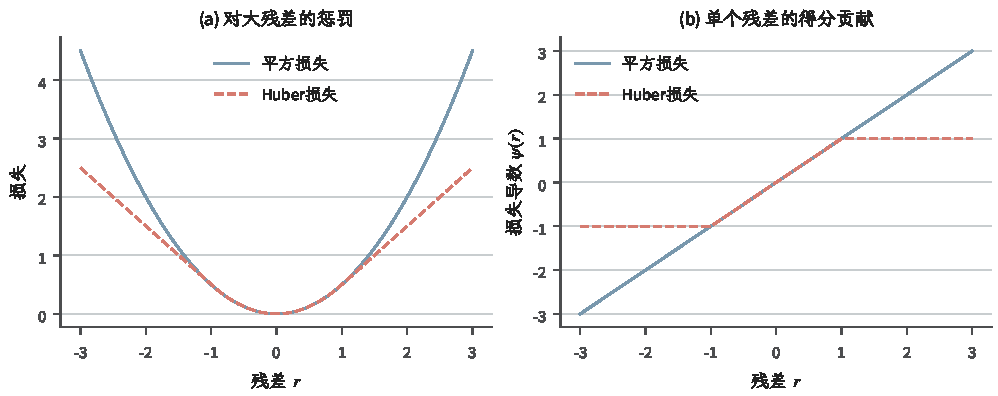
\includegraphics[width=\linewidth]{figures/math-preparation/probability-discrete/statistics-huber-loss.pdf}
  \caption{平方损失与阈值\(c=1\)的Huber损失（解析式教学图）。左图比较惩罚值，右图比较对残差的导数；Huber得分在\([-1,1]\)内截断。横轴是构造残差，不代表实测异常值分布。}
  \label{fig:statistics-huber-loss}
\end{figure*}

\subsection{偏差、方差与估计效率}
\label{sec:statistics-bias-efficiency}

\subsubsection{均方误差与一致性}

估计量的误差既来自系统偏移，也来自样本波动。对标量目标\(\theta\)，
\begin{align}
  \mathbb{E}[(\widehat\theta-\theta)^2]
  &=
  \mathbb{E}[(\widehat\theta-\mathbb{E}\widehat\theta
  +\mathbb{E}\widehat\theta-\theta)^2] \notag\\
  &=
  \operatorname{Var}(\widehat\theta)
  +\bigl(\mathbb{E}[\widehat\theta]-\theta\bigr)^2.
  \label{eq:statistics-mse-decomposition}
\end{align}
交叉项期望为零，因而均方误差等于方差加偏差平方。无偏不等于误差最小；少量偏差可能
换来更大的方差下降。

\begin{definition}[估计量的风险]
  \label{def:statistics-estimator-risk}
给定模型、目标泛函\(\tau\)和非负可测损失\(\ell\)，估计量的\term{风险}（risk）是
\[
  R_\theta(\widehat\tau)
  =\mathbb{E}_\theta[
    \ell(\widehat\tau(\bm Y),\tau(\theta))].
\]
它允许取\(+\infty\)，并随未知参数\(\theta\)变化。
\end{definition}
若\(\bm\theta\in\mathbb{R}^d\)并使用总平方误差，则
\[
  \mathbb{E}\lVert\widehat{\bm\theta}-\bm\theta\rVert_2^2
  =\operatorname{tr}\{\operatorname{Cov}(\widehat{\bm\theta})\}
   +\lVert\mathbb{E}\widehat{\bm\theta}-\bm\theta\rVert_2^2.
\]
这不是每个坐标风险的最大值，也不是任意方向风险。

在高斯位置例子中，取固定中心\(\mu_0\)并令
\(\widetilde\theta=a\overline Y+(1-a)\mu_0\)，则
\[
  \operatorname{MSE}_\theta(\widetilde\theta)
  =\frac{a^2\sigma^2}{n}+(1-a)^2(\mu_0-\theta)^2.
\]
当\(\theta\)接近\(\mu_0\)时，某些\(a<1\)可比无偏的样本均值具有更小有限样本
均方误差；远离中心时，收缩偏差又可能占主导。比较结论必须固定目标、样本量和损失。

当任意\(\epsilon>0\)都满足
\(\mathbb{P}_\theta(|\widehat\theta_n-\theta|>\epsilon)\to0\)时，称估计量
\term{一致}（consistent）。一致性只描述样本量趋于无穷的极限，不给出当前样本的
误差，也不排除有限样本偏差。若
\(\mathbb{E}_\theta[(\widehat\theta_n-\theta)^2]\to0\)，则称为均方一致；
Markov不等式说明均方一致推出依概率一致，反向结论没有额外一致可积性时并不成立。
对某些满足额外正则条件的估计量，还能进一步证明
\[
  \sqrt n(\widehat\theta_n-\theta)
  \xrightarrow{\mathrm d}\mathcal N(0,V).
\]
这项性质称为渐近正态，它需要另行建立，并不由一致性自动推出。

渐近展开经常同时出现确定的缩放因子和随机余项。不能用“每次取值都有限”代替余项控制：所需的是坏事件的概率能被同一常数压小。概率阶记号把这种控制与确定数列的阶区分开。
\begin{definition}[概率阶记号]
  \label{def:statistics-probability-order}
\term{概率有界}（bounded in probability）把“随机量不会随\(n\)逃向无穷”写成
可检验的概率条件。若对每个\(\epsilon>0\)，都存在有限常数\(M\)和整数\(n_0\)，使
\[
  \sup_{n\geq n_0}\mathbb{P}(|X_n|>M)<\epsilon,
\]
就记\(X_n=O_{\mathbb{P}}(1)\)。若\(X_n\to_{\mathbb{P}}0\)，则记
\(X_n=o_{\mathbb{P}}(1)\)。对确定正数列\(a_n\)，约定\(X_n=O_{\mathbb P}(a_n)\)与\(X_n=o_{\mathbb P}(a_n)\)分别表示\(X_n/a_n=O_{\mathbb P}(1)\)与\(X_n/a_n=o_{\mathbb P}(1)\)。
\end{definition}
依分布收敛的序列必然概率有界，但
\(O_{\mathbb{P}}(1)\)本身不指定唯一极限分布。

\subsubsection{线性无偏估计与Gauss--Markov定理}

无偏性约束了平均位置，却尚未比较方差。把单一信号推广为一组带噪线性观测：给定设计矩阵\(\bm X\in\mathbb R^{n\times d}\)，设
\begin{equation}
  \bm Y=\bm X\bm\theta+\bm\varepsilon,\qquad
  \mathbb E[\bm\varepsilon\mid\bm X]=\bm0,\qquad
  \operatorname{Cov}(\bm\varepsilon\mid\bm X)=\sigma^2\bm I_n,
  \quad\sigma^2>0.
  \label{eq:statistics-gauss-markov-model}
\end{equation}
不同观测的条件噪声方差相同且协方差为零；这里不要求独立或高斯噪声。列满秩使参数可识别，第~\ref{chap:linear-algebra}章的最小二乘解为
\(\widehat{\bm\theta}=(\bm X^\top\bm X)^{-1}\bm X^\top\bm Y\)。它是否在所有无偏估计中最佳，需要先限定比较类。
\begin{theorem}[Gauss--Markov定理]
  \label{thm:statistics-gauss-markov}
  在式~\eqref{eq:statistics-gauss-markov-model}下，若\(\bm X\)列满秩，则\(\widehat{\bm\theta}\)条件无偏，且
  \(\operatorname{Cov}(\widehat{\bm\theta}\mid\bm X)=\sigma^2(\bm X^\top\bm X)^{-1}\)。
  对任何条件于\(\bm X\)固定、对全部\(\bm\theta\)均无偏的线性估计\(\widetilde{\bm\theta}=\bm C\bm Y\)，有
  \[
    \operatorname{Cov}(\widetilde{\bm\theta}\mid\bm X)
    -\operatorname{Cov}(\widehat{\bm\theta}\mid\bm X)\succeq\bm0.
  \]
\end{theorem}
\begin{proof}
记\(\bm C_0=(\bm X^\top\bm X)^{-1}\bm X^\top\)，于是\(\bm C_0\bm X=\bm I_d\)。直接对\(\bm C_0\bm Y\)求条件均值和协方差，得到无偏性及所述协方差。任一线性估计对所有参数无偏，等价于\(\bm C\bm X=\bm I_d\)。写\(\bm C=\bm C_0+\bm D\)，则\(\bm D\bm X=\bm0\)，从而
\[
  \bm C_0\bm D^\top
  =(\bm X^\top\bm X)^{-1}(\bm D\bm X)^\top=\bm0.
\]
展开\(\sigma^2\bm C\bm C^\top\)时两个交叉项都为零，故协方差之差为\(\sigma^2\bm D\bm D^\top\)。对任意向量\(\bm a\)，其二次型为\(\sigma^2\|\bm D^\top\bm a\|_2^2\geq0\)，即得半正定结论。
\end{proof}
半正定比较表示任意线性组合\(\bm a^\top\bm\theta\)的方差都不更大，强于只比较各坐标方差。定理的比较类是线性无偏估计，不排除前面那类有偏收缩估计获得更小均方误差，也不把异方差或相关噪声包含进来。

若\(\bm X=\bm1_n\)，参数就是共同均值，最小二乘退化为样本平均。任一无偏加权平均\(\sum_i a_iY_i\)满足\(\sum_i a_i=1\)；写\(a_i=1/n+b_i\)，则\(\sum_i b_i=0\)，其方差为
\(\sigma^2\sum_i a_i^2=\sigma^2/n+\sigma^2\sum_i b_i^2\)。额外的不均衡权重只增加方差，给出矩阵证明的一个可逐项核对的特例。

\subsubsection{渐近正态与Delta方法}

样本均值给出渐近正态的基本例子。若
\(Y_1,\ldots,Y_n\)独立同分布，且
\(\mathbb{E}[Y_i]=\theta\)、
\(0<\operatorname{Var}(Y_i)=\sigma^2<\infty\)，则中心极限定理给出
\[
  \sqrt n(\overline Y-\theta)
  \xrightarrow{\mathrm d}\mathcal N(0,\sigma^2).
\]
因此均值的渐近正态只需要有限方差，不要求观测本身服从高斯分布；在高斯位置模型中，
这个正态分布关系对每个有限\(n\)已经精确成立。

\begin{theorem}[Slutsky定理]
  \label{thm:statistics-slutsky}
  若\(X_n\xrightarrow{\mathrm d}X\)，且
  \(Y_n\xrightarrow{\mathbb{P}}c\)，其中\(c\)为常数，则
  \[
    X_n+Y_n\xrightarrow{\mathrm d}X+c,\qquad
    X_nY_n\xrightarrow{\mathrm d}cX.
  \]
  若\(c\neq0\)，还有
  \(X_n/Y_n\xrightarrow{\mathrm d}X/c\)。特别地，若
  \(R_n=o_{\mathbb{P}}(1)\)，则
  \(X_n+R_n\xrightarrow{\mathrm d}X\)。
\end{theorem}

Slutsky定理允许把收敛到常数的标准误、归一化因子或余项代入渐近分布。它不表示两个一般
随机极限可以忽略联合分布；关键条件是其中一个序列依概率收敛到常数。

\begin{theorem}[Delta方法]
\label{thm:statistics-delta-method}
若
\(\sqrt n(\widehat\theta_n-\theta)\xrightarrow{\mathrm d}\mathcal N(0,V)\)，
且\(g\)在\(\theta\)处可微，则
\[
  \sqrt n\bigl(g(\widehat\theta_n)-g(\theta)\bigr)
  \xrightarrow{\mathrm d}
  \mathcal N\bigl(0,g'(\theta)^2V\bigr).
\]
\end{theorem}

\begin{proof}
记
\[
  Z_n=\sqrt n(\widehat\theta_n-\theta),
  \qquad
  Z\sim\mathcal N(0,V).
\]
先补出证明所需的两条概率阶规则。由\(Z_n\xrightarrow{\mathrm d}Z\)，对任意
\(\epsilon>0\)，可取充分大的\(M\)使
\(\mathbb{P}(|Z|\geq M)<\epsilon/2\)。依分布收敛的闭集上界给出
\[
  \limsup_{n\to\infty}\mathbb{P}(|Z_n|\geq M)
  \leq \mathbb{P}(|Z|\geq M)<\epsilon/2,
\]
所以\(Z_n=O_{\mathbb{P}}(1)\)。此外，若
\(A_n=o_{\mathbb{P}}(1)\)、\(B_n=O_{\mathbb{P}}(1)\)，则对任意
\(\eta,\epsilon>0\)，先取\(M\)使大样本下
\(\mathbb{P}(|B_n|>M)<\epsilon/2\)，再取充分大的\(n\)使
\(\mathbb{P}(|A_n|>\eta/M)<\epsilon/2\)。于是
\[
  \mathbb{P}(|A_nB_n|>\eta)
  \leq
  \mathbb{P}(|B_n|>M)
  +\mathbb{P}(|A_n|>\eta/M)
  <\epsilon,
\]
即\(o_{\mathbb{P}}(1)O_{\mathbb{P}}(1)=o_{\mathbb{P}}(1)\)。

特别地，
\(\widehat\theta_n-\theta=n^{-1/2}Z_n=o_{\mathbb{P}}(1)\)，所以估计量依概率一致。
Taylor展开给出
\[
  g(\widehat\theta_n)-g(\theta)
  =g'(\theta)(\widehat\theta_n-\theta)
   +r_n(\widehat\theta_n-\theta),
\]
其中一致性与可微性保证\(r_n=o_{\mathbb{P}}(1)\)。乘以\(\sqrt n\)后，
余项是
\(r_nZ_n=o_{\mathbb{P}}(1)\)。主项由假设依分布收敛，再用Slutsky定理即得结论。
\end{proof}

回到上述有限方差样本均值，若\(\theta>0\)，取\(g(\theta)=\log\theta\)，
便有渐近方差
\(\sigma^2/\theta^2\)。若\(g'(\theta)=0\)，一阶Delta方法仍成立，但只给出零方差的退化极限；要描述非退化波动，需要更高阶展开与新的缩放。若\(g\)在目标点不可微，才不能直接应用上述定理。

一般估计方程也给出一个正则渐近式。若
\(\mathbb{E}[\psi(Y,\theta_0)]=0\)，记
\[
  A=\mathbb{E}[\partial_\theta\psi(Y,\theta_0)],
  \qquad B=\operatorname{Var}(\psi(Y,\theta_0)),
\]
且一致性、可微性、矩条件和中心极限定理所需条件成立，则在\(\theta_0\)附近展开
样本估计方程可得
\[
  \sqrt n(\widehat\theta-\theta_0)
  =
  -A^{-1}\frac1{\sqrt n}\sum_{i=1}^n\psi(Y_i,\theta_0)
  +o_{\mathbb{P}}(1),
\]
故极限方差为\(A^{-2}B\)。多维情形相应为
\(A^{-1}B(A^{-1})^\top\)，常称夹心协方差。模型正确的光滑似然在正则条件下可用
信息恒等式化简它；模型失配时\(A\)与\(B\)通常不再是同一个信息量，夹心两侧不能省略。

\subsubsection{得分、Fisher信息与效率界}

均方误差评价一个给定估计量，效率界进一步询问同一观测模型允许的估计精度。
这里用对数似然的导数记录数据对参数的局部辨别能力；Fisher信息与统计几何章共用
同一个分布对象，本小节将它用于无偏估计的误差下界，而非另建一种曲率矩阵。

\term{Fisher信息}（Fisher information）衡量观测分布对参数局部变化的敏感程度。

\begin{definition}[Fisher信息矩阵]
\label{def:information-fisher-matrix}
对开参数域上的受共同测度支配模型\(p_{\bm\theta}\)，固定参数内点\(\bm\theta\)。假设在\(P_{\bm\theta}\)-几乎每个\(x\)处，\(p_{\bm\theta}(x)>0\)且\(\log p_{\bm\theta}(x)\)关于参数可微。定义得分向量\(\bm s_{\bm\theta}(x)=\nabla_{\bm\theta}\log p_{\bm\theta}(x)\)；若\(\mathbb E_{\bm\theta}\lVert\bm s_{\bm\theta}(X)\rVert_2^2<\infty\)，该点的\term{Fisher信息矩阵}定义为
\begin{equation}
  \bm{F}(\bm{\theta})
  =
  \mathbb{E}_{\bm{\theta}}\!\left[
    \bm{s}_{\bm{\theta}}(X)
    \bm{s}_{\bm{\theta}}(X)^{\top}
  \right].
  \label{eq:information-fisher-matrix}
\end{equation}
它是得分外积在模型分布下的平均，必为半正定矩阵。标量参数时退化为得分平方的期望；这个定义本身不要求它等于负对数似然的期望Hessian，后一个恒等式还需正则条件。
\end{definition}

下面固定一组足以支持常用恒等式的正则条件：参数位于开区间，所有密度相对于共同参考
测度定义并具有共同正支持；密度关于参数二次连续可微；目标参数邻域内的一、二阶密度
导数分别受可积函数控制；得分二阶矩有限。对得分
\(s_\theta(Y)=\partial_\theta\log p_\theta(Y)\)，这些条件允许交换微分与积分，于是
\[
  \mathbb{E}_\theta[s_\theta(Y)]
  =\int\partial_\theta p_\theta(y)\,\mathrm dy
  =\partial_\theta1=0.
\]
再由
\(\partial_\theta^2\log p_\theta
=(\partial_\theta^2p_\theta)/p_\theta-s_\theta^2\)积分，得到
\[
  \mathcal I(\theta)
  =\mathbb{E}_\theta[s_\theta(Y)^2]
  =-\mathbb{E}_\theta[\partial_\theta^2\log p_\theta(Y)].
\]
高斯位置观测的单样本信息为\(1/\sigma^2\)，\(n\)个独立观测的信息相加为
\(n/\sigma^2\)。下文记整批样本的得分为
\(s_\theta(\bm Y)=\sum_{i=1}^n s_\theta(Y_i)\)。

\begin{theorem}[Cramér--Rao下界]
\label{thm:statistics-cramer-rao}
设\(Y_1,\ldots,Y_n\)独立同分布于\(p_\theta\)，并且上述正则条件成立且单样本
Fisher信息满足\(0<\mathcal I(\theta)<\infty\)。若\(\widehat\tau\)对可微目标
\(\tau(\theta)\)无偏、二阶矩有限，且其期望可对参数求导并移入积分，则
\[
  \operatorname{Var}_\theta(\widehat\tau)
  \geq\frac{\tau'(\theta)^2}{n\mathcal I(\theta)}.
\]
\end{theorem}

\begin{proof}
由无偏性\(\mathbb{E}_\theta[\widehat\tau]=\tau(\theta)\)对参数求导，并把导数移入积分，
得到
\[
  \tau'(\theta)
  =\mathbb{E}_\theta[
    (\widehat\tau-\tau(\theta))s_\theta(\bm Y)].
\]
Cauchy--Schwarz不等式给出
\[
  \tau'(\theta)^2\leq
  \operatorname{Var}_\theta(\widehat\tau)
  \operatorname{Var}_\theta(s_\theta(\bm Y))
  =
  \operatorname{Var}_\theta(\widehat\tau)n\mathcal I(\theta),
\]
整理即得结论。
\end{proof}

这个界不是所有估计问题的普遍极限。参数位于边界、支持依赖参数、模型不可识别或
Fisher信息奇异时，证明中的求导和除法可能失效；有偏估计量也要使用相应的偏差版本。
对\(\bm\theta\in\mathbb{R}^p\)和可微目标
\(\bm\tau(\bm\theta)\in\mathbb{R}^q\)，向量参数的正则版本为
\[
  \operatorname{Cov}_{\bm\theta}(\widehat{\bm\tau})
  \succeq
  \bm J_\tau(\bm\theta)\,
  \bm{\mathcal I}_n(\bm\theta)^{-1}\,
  \bm J_\tau(\bm\theta)^\top,
\]
其中\(\bm J_\tau\in\mathbb{R}^{q\times p}\)是目标映射的Jacobian，
\(\bm{\mathcal I}_n\)是整批样本的Fisher信息矩阵。这里要求信息矩阵可逆，
但Jacobian可以是矩形或降秩矩阵；估计参数本身时
\(\bm\tau(\bm\theta)=\bm\theta\)，故\(\bm J_\tau=\bm I_p\)。矩阵结论也不能由
逐坐标标量界直接拼接得到。

\subsection{Bayes估计与层次共享}
\label{sec:statistics-bayes-hierarchy}

\subsubsection{先验、后验与后验预测}

频率学派把参数固定而把样本看作随机。Bayes方法另给参数指定先验
\(\pi(\theta)\)，观测后用
\[
  \pi(\theta\mid\bm y)
  =
  \frac{p(\bm y\mid\theta)\pi(\theta)}
       {\int p(\bm y\mid u)\pi(u)\,\mathrm du}
\]
得到\term{后验分布}（posterior distribution）。它把似然提供的数据证据与先验
假设合并。这个公式要求分母，即模型证据，严格为正且有限；否则右侧不能定义概率分布。

后验均值最小化后验平方损失。事实上，对任意行动\(a\)，令
\(m=\mathbb{E}[\theta\mid\bm y]\)，则
\[
  \mathbb{E}[(\theta-a)^2\mid\bm y]
  =\operatorname{Var}(\theta\mid\bm y)+(a-m)^2.
\]
后验中位数则最小化后验绝对损失，其理由与前文总体中位数的左右方向导数相同。最大后验
估计只选择相对于指定参考测度的密度峰值；非线性重参数化会引入Jacobian因子，因此峰值
位置一般不保持不变。三种Bayes行动不必相同。

设
\[
  Y_i\mid\theta\overset{\mathrm{iid}}{\sim}\mathcal N(\theta,\sigma^2),
  \qquad
  \theta\sim\mathcal N(\mu_0,\tau_0^2).
\]
配方后得到共轭更新
\[
  \theta\mid\bm y
  \sim\mathcal N(\mu_n,\tau_n^2),\qquad
  \tau_n^{-2}=\tau_0^{-2}+n\sigma^{-2},
\]
\[
  \mu_n=\tau_n^2
  \left(\frac{\mu_0}{\tau_0^2}+\frac{n\overline y}{\sigma^2}\right).
\]
后验均值是先验均值与样本均值按精度加权的折中。若要预测新读数，还要积分掉参数：
\[
  Y_{n+1}\mid\bm y
  \sim\mathcal N(\mu_n,\sigma^2+\tau_n^2).
\]
其中\(\tau_n^2\)是参数不确定性，\(\sigma^2\)是新观测自身的噪声。

离散比例也有同样的共轭结构。若
\(Y_i\mid p\overset{\mathrm{iid}}{\sim}\operatorname{Bernoulli}(p)\)且
\(p\sim\operatorname{Beta}(a,b)\)，观察到\(s=\sum_iY_i\)个成功后，
\[
  p\mid\bm y\sim\operatorname{Beta}(a+s,b+n-s).
\]
对\(K\)类计数\((n_1,\ldots,n_K)\)，Dirichlet先验
\(\operatorname{Dirichlet}(\alpha_1,\ldots,\alpha_K)\)相应更新为
\(\operatorname{Dirichlet}(\alpha_1+n_1,\ldots,\alpha_K+n_K)\)。这些更新依赖
给定比例后的条件独立抽样；过度离散或来源相关时，简单加计数会夸大信息量。

\subsubsection{层次模型与部分汇聚}

多个设备、标注者或任务的数据量很不均衡时，可令
\[
  \theta_g\mid\mu,\tau^2\sim\mathcal N(\mu,\tau^2),\qquad
  Y_{g,i}\mid\theta_g\sim\mathcal N(\theta_g,\sigma_g^2).
\]
这里假设给定\((\mu,\tau^2)\)后各组参数\(\theta_g\)条件独立，并且给定全部组参数后，
所有\(Y_{g,i}\)也条件独立。若\(\mu,\tau^2,\sigma_g^2\)暂视为已知，且第\(g\)组有
\(n_g\)个观测，则
\[
  \theta_g\mid\bm y_g,\mu,\tau^2
  \sim\mathcal N(m_g,V_g),\qquad
  V_g^{-1}=\tau^{-2}+n_g\sigma_g^{-2},
\]
\[
  m_g
  =V_g\left(\frac{\mu}{\tau^2}
    +\frac{n_g\overline y_g}{\sigma_g^2}\right).
\]
固定超参数时，第\(g\)组后验只依赖\(\bm y_g\)以及外部给定的共同中心和尺度；
小样本群组会更强地向共同中心\(\mu\)收缩，其他组数据尚未进入该后验。
当用全部群组数据估计共同超参数，或在完整Bayes模型中对其后验积分时，其他组数据才会
通过共同超参数间接改变第\(g\)组的推断，从而形成组间信息共享。
\(\tau^2\to0\)接近完全汇聚，\(\tau^2\to\infty\)接近各组独立估计，有限正尺度给出
部分汇聚。若超参数由同一数据估计，这是经验Bayes；若继续给它们指定先验，推断对象还
包括超参数后验。
这不是免费增加数据，而是加入“群组来自共同总体”的结构假设。若群组机制不同或先验
尺度过窄，收缩会掩盖真实差异。先验由研究者指定并不把固定物理参数变成随机生成的
事实；Bayes概率表达的是模型内部的不确定性。

\section{区间、检验与数据选择}
\label{sec:stats-uncertainty-testing-selection}

点估计不能表达证据的精度。本节先把误差转成区间和检验，再说明抽样分布未知时怎样用重采样近似它。
这些保证通常针对预先指定的分析；比较多个候选或持续查看结果会改变被报告结果的产生规则，
因此还要把选择和停止纳入误差控制。

\subsection{区间、分位数与预测范围}
\label{sec:statistics-intervals-quantiles}

\subsubsection{置信、可信与预测区间}

点估计没有说明误差尺度。覆盖区间需要先说明概率来自哪一次随机化，以及要覆盖的对象。
\begin{definition}[置信、可信与预测覆盖]
  \label{def:statistics-interval-coverage}
  取\(0<\alpha<1\)。\term{置信区间}（confidence interval）是一项重复抽样
程序：若每次按同一制度抽样并构造\(C(\bm Y)\)，则对模型中的每个\(\theta\)都有
\[
  \mathbb{P}_\theta\{\theta\in C(\bm Y)\}\geq1-\alpha.
\]
频率学派参数始终视作固定值；数据固定后，得到的区间也固定，不能把它解释为“以\(1-\alpha\)
概率包含参数”。Bayes\term{可信区间}（credible interval）则在给定数据和模型后
满足\(\mathbb{P}(\theta\in C\mid\bm y)\geq1-\alpha\)，其数值依赖先验；连续后验常可取到等号，离散后验可能只能给出更大的覆盖概率。
\term{预测集合}（prediction set）把覆盖对象改成未来结果，在规定的训练样本与未来
观测联合分布下要求
\(\mathbb{P}\{Y_{n+1}\in C(\bm Y)\}\geq1-\alpha\)。三者的概率分别来自重复样本、
参数后验和未来观测，不能只按区间端点的外观解释。
\end{definition}

在独立同分布的高斯位置模型中，若方差已知，则
\[
  \frac{\overline Y-\theta}{\sigma/\sqrt n}\sim\mathcal N(0,1),
\]
因而双侧置信区间为
\[
  \overline Y\pm z_{1-\alpha/2}\frac{\sigma}{\sqrt n}.
\]
若未来读数独立于已有样本并来自同一模型，预测误差
\(Y_{n+1}-\overline Y\)的方差是
\(\sigma^2(1+1/n)\)，所以相同模型下的双侧预测区间为
\[
  \overline Y\pm z_{1-\alpha/2}\sigma\sqrt{1+\frac1n}.
\]
预测区间因此比参数区间更宽。参数区间覆盖固定位置参数，预测区间覆盖尚未发生的随机
结果；把参数标准误直接用于预测会遗漏新观测噪声。

\begin{example}[贯穿本章的传感器校准数据]
  \label{ex:statistics-running-sensor-calibration}
  考虑一组教学构造的传感器校准数据。共有\(n=25\)个独立响应，样本均值为
  \(\overline y=10.4\)，已知单次测量噪声标准差为\(\sigma=2\)，样本经验二阶中心矩
  为
  \[
    \frac1{25}\sum_{i=1}^{25}(y_i-\overline y)^2=4.
  \]
  在\(95\%\)水平下，\(z_{0.975}\approx1.96\)。位置参数的置信区间为
  \[
    10.4\pm1.96\frac{2}{5}
    =[9.62,11.18],
  \]
  而下一次读数的预测区间为
  \[
    10.4\pm1.96\times2\sqrt{1+\frac1{25}}
    =[6.40,14.40].
  \]
  两个区间中心相同，宽度差异完全来自覆盖对象不同。

  后文还要估计响应关于校准输入\(x\)的局部均值。靠近左边界\(x_0=0\)的三个观测为
  \[
    (x_i,y_i)=(0,9),(1,11),(3,13),
  \]
  在一个给定带宽下对应核权重\(1,0.75,0.25\)。这些汇总量会在Bootstrap、带宽选择
  和局部回归中继续使用；它们是用于复核方法差别的构造数值，不是实测性能报告。
\end{example}

图~\ref{fig:statistics-mean-prediction-width}显示这一区分在样本量增长时仍然存在：均值标准误按\(n^{-1/2}\)减小，而未来单次读数的噪声不会因历史样本增多而消失。因此收集更多校准数据会把位置参数确定得更精确，却不能把一个有噪声的新读数限制到同样窄的范围。

\begin{figure}[htbp]
  \centering
  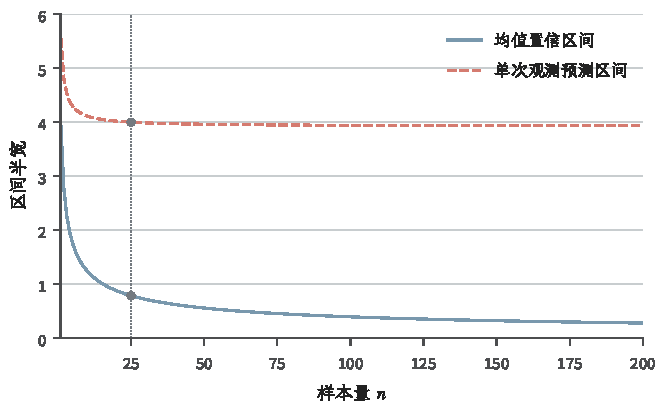
\includegraphics[width=\linewidth]{figures/math-preparation/probability-discrete/statistics-mean-prediction-width.pdf}
  \caption{已知\(\sigma=2\)的独立高斯位置模型中，两类区间半宽随样本量变化（解析式教学图）。使用四舍五入分位数\(1.96\)，蓝实线为\(1.96\sigma/\sqrt n\)，红虚线为\(1.96\sigma\sqrt{1+1/n}\)。灰竖线标出例~\ref{ex:statistics-running-sensor-calibration}的\(n=25\)，没有对任何实测数据重复抽样。}
  \label{fig:statistics-mean-prediction-width}
\end{figure}

\begin{table}[htbp]
  \centering
  \begin{tabular}{p{0.16\linewidth}p{0.29\linewidth}p{0.43\linewidth}}
    \toprule
    类型 & 覆盖对象 & 概率来源与必要条件\\
    \midrule
    置信区间 & 固定总体参数 & 同一抽样制度下重复构造区间的覆盖率\\
    可信区间 & 给定数据的参数后验 & 指定先验与似然形成的后验概率；不自动具有频率覆盖\\
    预测区间 & 尚未观测的随机结果 & 训练样本与未来观测的联合分布；须包含新观测波动\\
    \bottomrule
  \end{tabular}
  \caption{三类区间的覆盖对象与概率来源。区间形式相似时，仍须从所覆盖的对象解释结论。}
  \label{tab:statistics-interval-objects}
\end{table}

方差未知时，用
\[
  S^2=\frac1{n-1}\sum_{i=1}^n(Y_i-\overline Y)^2
\]
估计\(\sigma^2\)。高斯独立样本下，
\[
  \frac{\overline Y-\theta}{S/\sqrt n}\sim t_{n-1},
\]
所以把高斯分位数换成\(t\)分位数可得到精确置信区间。这里的精确性依赖高斯性；
一般分布下它通常只是渐近近似。样本很小且分布偏斜、重尾时，机械使用该区间可能同时
破坏中心和尾部覆盖。

双侧区间与双侧检验在相同模型、显著性水平和统计量下互为反演：若
\(\theta_0\)不在\(1-\alpha\)置信区间内，就拒绝\(H_0:\theta=\theta_0\)。
这种对应关系要求两者使用相同标准误与尾部规则。选择后区间、单侧检验或离散检验中，
不能只凭表面上的阈值照搬这一关系。

\subsubsection{分位数、次序统计量与边际覆盖}

\term{\(q\)分位数}（quantile）可定义为
\[
  F^{-1}(q)=\inf\{y:F(y)\geq q\},\qquad 0<q<1.
\]
这个广义逆为给定的\(F\)和\(q\)选出唯一的下分位数。更一般地，所有满足分位数
不等式的点组成集合
\[
  \mathcal Q_q=\{a:F(a^-)\leq q\leq F(a)\}.
\]
当\(F\)在水平\(q\)上存在平坦区间时，这个集合可能包含多个点；上述广义逆约定选取
其中的下端代表。
对次序统计量\(Y_{(1)}\leq\cdots\leq Y_{(n)}\)，经验分位数由相应秩位置给出。
若\(Y_1,\ldots,Y_n\)是来自连续分布\(F\)的独立同分布样本，则
\(F(Y_{(k)})\)服从
\(\operatorname{Beta}(k,n+1-k)\)，因此可以用秩而不是高斯近似构造分位数区间。
对离散或混合分布，跳跃与平坦区间都要求覆盖计算保留定义中的不等式方向。

总体分位数平均了不同输入；若不同\(x\)对应不同位置或尾部，还需要按输入报告分位数。
\begin{definition}[条件分位数]
  \label{def:statistics-conditional-quantile}
给定\(Y\)关于\(X=x\)的正则条件分布，记\(F_x(y)=\mathbb P(Y\leq y\mid X=x)\)。对\(0<q<1\)，下条件\(q\)分位数为\(F_x^{-1}(q)=\inf\{y:F_x(y)\geq q\}\)；完整条件分位数集合为\(\{a:F_x(a^-)\leq q\leq F_x(a)\}\)。这些对象随条件分布版本确定，并按\(P_X\)-几乎处处意义理解。
\end{definition}
条件分位数可由\term{分位数回归}（quantile regression）估计。假设\(Y\)可积，使下面损失的条件期望对几乎每个\(x\)有限。令
\[
  \rho_q(u)=u\bigl(q-\mathbb{I}_{\{u<0\}}\bigr),
\]
则条件\(q\)分位数最小化
\(\mathbb{E}[\rho_q(Y-a)\mid X=x]\)。固定\(x\)并记条件分布函数为\(F\)，目标对
\(a\)的次梯度区间是
\[
  [F(a^-)-q,\ F(a)-q].
\]
因此最优点恰好满足\(F(a^-)\leq q\leq F(a)\)；连续严格递增时才简化为
\(F(a)=q\)。因此分位数损失的最小点集合正是\(\mathcal Q_q\)，可能不唯一，
而\(F^{-1}(q)\)仍是其中按约定选出的单个代表。分位数回归直接估计条件分布的位置，
不要求误差为高斯或方差恒定。

第~\ref{sec:probability-exchangeability-conformal-ranks}节的共形预测用可交换观测的
秩构造有限样本预测集。具体地，先用与校准集、待预测点分离的训练数据固定评分函数，
再由\(m\)个校准分数\(S_1,\ldots,S_m\)取
\[
  k=\left\lceil(m+1)(1-\alpha)\right\rceil,\qquad
  \widehat q=S_{(k)}.
\]
若\(k=m+1\)，约定阈值为\(+\infty\)；并列分数采用保守的“分数不超过阈值”规则。
校准分数与新分数可交换时，新分数的秩在\(m+1\)个位置上对称，因而分割共形的边际
覆盖结论为
\[
  \mathbb{P}\{Y_{n+1}\in C(X_{n+1})\}\geq1-\alpha.
\]
概率同时平均了不同\(X\)区域。它不推出每个群组或每个
\(x\)都达到同样覆盖率；分组校准只能对预先规定且样本充分的群组提供相应保证，精细到
每个连续条件点的无分布精确覆盖通常不可得。

\subsection{假设检验与误差控制}
\label{sec:statistics-testing-errors}

\subsubsection{检验、p值与区间反演}

区间描述目标的可能范围，\term{假设检验}（hypothesis testing）则检查数据与一个
命题是否相容。
\begin{definition}[随机化检验函数]
  \label{def:statistics-randomized-test-function}
  若单个观测的可测空间为\(\mathcal{Y}\)，则
  \term{随机化检验函数}（randomized test function）是可测映射
  \[
    \varphi:\mathcal{Y}^n\to[0,1].
  \]
  观察到\(\bm{Y}=\bm{y}\)后，检验以概率\(\varphi(\bm{y})\)拒绝原假设。等价地，可另取
  独立的\(U\sim\operatorname{Unif}(0,1)\)，并在
  \(U\leq\varphi(\bm{y})\)时拒绝。只取\(0,1\)值的检验是非随机化特例，其拒绝域为
  \(R=\{\bm{y}:\varphi(\bm{y})=1\}\)。
\end{definition}

原假设\(H_0\)指定被控制误报的情形。检验的大小与参数\(\theta\)下的功效分别为
\[
  \sup_{\theta\in H_0}\mathbb{E}_\theta[\varphi(\bm Y)],
  \qquad
  \mathbb{E}_\theta[\varphi(\bm Y)].
\]
水平为\(\alpha\)要求
\[
  \sup_{\theta\in H_0}
  \mathbb{E}_\theta[\varphi(\bm Y)]
  \leq\alpha.
\]
在\(H_0\)为真时拒绝是第一类错误；在备择\(H_1\)为真时不拒绝是第二类错误。
对非随机化检验，这些期望分别退化为拒绝域概率。效应量描述差异有多大，样本量则影响
能否把该差异从噪声中区分出来。

\term{\(p\)值}（\(p\)-value）是在原假设下，得到至少与当前统计量同样极端结果的
概率。
\begin{definition}[有效p值]
  \label{def:statistics-valid-p-value}
  一个取值于\([0,1]\)的可测统计量\(p(\bm Y)\)是复合原假设\(H_0\)下的有效\(p\)值，若对每个
\(u\in[0,1]\)都有
\[
  \sup_{\theta\in H_0}\mathbb{P}_\theta\{p(\bm Y)\leq u\}\leq u.
\]
\end{definition}
这项零假设下的超均匀性质才保证按阈值\(\alpha\)拒绝时控制第一类错误。观察到的
\(p\)值不是原假设为真的概率，也不是效应量。仍取已知\(\sigma\)的高斯位置模型，
检验\(H_0:\theta=0\)时
\[
  Z=\frac{\sqrt n\,\overline Y}{\sigma},\qquad
  p=2\{1-\Phi(|Z|)\}.
\]
若\(\theta=\delta\)，双侧检验功效为
\[
  \mathbb{P}_\delta(|Z|>z_{1-\alpha/2})
  =
  1-\Phi\left(z_{1-\alpha/2}-\frac{\sqrt n\delta}{\sigma}\right)
  +\Phi\left(-z_{1-\alpha/2}-\frac{\sqrt n\delta}{\sigma}\right).
\]
小样本下“不显著”可能只表示功效不足。相同效应量在更大\(n\)下会得到更小的
\(p\)值。

检验族还可反演为置信集合。对每个候选值\(\theta_0\)，设
\(\varphi_{\theta_0}(\bm Y)\in\{0,1\}\)是水平不超过\(\alpha\)的检验，并定义
\[
  C(\bm Y)=\{\theta_0:\varphi_{\theta_0}(\bm Y)=0\}.
\]
当真实值为\(\theta\)时，
\[
  \mathbb{P}_\theta\{\theta\notin C(\bm Y)\}
  =\mathbb{P}_\theta\{\varphi_\theta(\bm Y)=1\}\leq\alpha,
\]
所以\(C\)具有至少\(1-\alpha\)覆盖率。这里必须对同一模型、同一尾部规则和同一
标准误反演；选择后换检验或只挑有利方向会破坏证明。

\begin{example}[同一效应量下的证据与功效]
\label{ex:statistics-evidence-power-same-effect}
设噪声标准差已知为\(\sigma=2\)，观测均值为\(\overline y=1\)，检验
\(H_0:\theta=0\)。当\(n=4\)时，\(Z=1\)，双侧\(p\)值约为\(0.317\)；
当\(n=100\)时，\(Z=5\)，双侧\(p\)值小于\(10^{-6}\)。两次实验报告的标准化
效应\(\overline y/\sigma=0.5\)相同，证据强度却因标准误不同而变化。

若真实值确为\(\delta=1\)，显著性水平为\(0.05\)，则\(n=4\)时双侧检验功效约为
\[
  1-\Phi(1.96-1)+\Phi(-1.96-1)\approx0.17.
\]
此时未拒绝原假设并不支持“差异为零”。若实际问题把绝对差异不超过\(0.2\)视为等效，
还需要针对\(\Delta=0.2\)设计等效检验；当前样本对这个更严格目标几乎没有辨识力。
\end{example}

\subsubsection{似然比排序与Neyman–Pearson引理}

下面的经典引理给出两个简单假设之间的最强检验\scite{math-lehmann2005testing}
\begin{theorem}[Neyman--Pearson引理]
\label{thm:statistics-neyman-pearson}
对两个完全指定的简单假设\(H_0:P=P_0\)与\(H_1:P=P_1\)，设
\(P_1\ll P_0\)，似然比为\(\Lambda=\mathrm dP_1/\mathrm dP_0\)。在所有大小
不超过\(\alpha\)的检验中，拒绝大似然比并在边界适当随机化的检验具有最大功效。
\end{theorem}

\begin{proof}
取常数\(c\)与边界随机化概率，使检验\(\varphi^\star\)满足
\(\mathbb{E}_0[\varphi^\star]=\alpha\)，并在\(\Lambda>c\)时拒绝、在
\(\Lambda<c\)时接受。对任意\(\mathbb{E}_0[\varphi]\leq\alpha\)的检验，
\[
  (\varphi^\star-\varphi)(\Lambda-c)\geq0
\]
逐点成立，因为\(\varphi^\star\)在\(\Lambda>c\)处取最大允许值，在
\(\Lambda<c\)处取最小允许值。对\(P_0\)积分得到
\[
  \mathbb{E}_1[\varphi^\star-\varphi]
  \geq c\,\mathbb{E}_0[\varphi^\star-\varphi]\geq0.
\]
所以\(\varphi^\star\)的备择拒绝概率不小于任何同大小检验。
\end{proof}

这个结论只直接覆盖两个简单假设。复合假设需要处理未知参数，不一定存在一致最强检验。
在隐私攻击审计中，\(P_0\)与\(P_1\)可分别表示目标记录不在与在训练集时的输出分布；
似然比给出理想攻击排序，但实际审计还要估计这两个分布并计入选择偏差。

\subsubsection{列联表、渐近检验与不同命题}

两个分类变量的列联表中，原假设为独立时，期望格数是
\[
  E_{r,c}=\frac{N_{r,\cdot}N_{\cdot,c}}{N},\qquad
  X^2=\sum_{r,c}\frac{(N_{r,c}-E_{r,c})^2}{E_{r,c}}.
\]
在独立抽样、固定维数且期望格数不过小时，
\(X^2\)近似服从自由度\((R-1)(C-1)\)的卡方分布。稀疏格数会破坏近似，可合并有
科学意义的类别或使用精确、置换方法。条件独立检验还要控制第三个变量；把样本简单切成
大量小层会带来新的稀疏性，不能由普通卡方检验自动解决。

差异检验把“无差异”放在原假设中。等效性检验先给出有实际含义的可接受差异界
\(\Delta>0\)。记\(\delta=\theta_A-\theta_B\)，两个单侧检验（two one-sided
tests, TOST）把不等效原假设写成两个集合的并：
\[
  H_0=H_{0,L}\cup H_{0,U},
  \qquad
  H_{0,L}:\delta\leq-\Delta,
  \qquad
  H_{0,U}:\delta\geq\Delta.
\]
对应备择为\(-\Delta<\delta<\Delta\)。TOST只有在水平\(\alpha\)的下侧检验拒绝
\(H_{0,L}\)，并且水平\(\alpha\)的上侧检验也拒绝\(H_{0,U}\)时，才拒绝总体原假设。
例如，若\(\widehat\delta\)的标准误为\(s\)，且标准化统计量服从相应正态近似，
拒绝条件为
\begin{equation}
  \frac{\widehat\delta+\Delta}{s}>z_{1-\alpha}
  \quad\text{且}\quad
  \frac{\widehat\delta-\Delta}{s}<z_{\alpha}.
  \label{eq:statistics-tost-rejection}
\end{equation}
这等价于把双侧\(1-2\alpha\)置信区间完整放入
\((-\Delta,\Delta)\)。总体第一类错误并非\(2\alpha\)：只要
\(\delta\in H_0\)，至少有一个单侧原假设为真，而总体拒绝事件包含在拒绝这个真原假设
的事件中，所以其概率至多为\(\alpha\)。非劣效检验只排除一个方向，例如
\(H_0:\delta\leq-\Delta\)。未拒绝差异检验的零假设不等于证明等效。

\subsection{重采样与经验不确定性}
\label{sec:statistics-resampling}

\subsubsection{Bootstrap与抽样分布近似}

复杂估计量的抽样分布难以解析计算时，可以让经验数据模拟重复抽样。
\term{Bootstrap}从经验分布
\(\widehat P_n=n^{-1}\sum_i\Delta_{Y_i}\)有放回抽取\(n\)个观测，并重新计算
\(\widehat\tau^\ast\)。条件于原样本的
\(\widehat\tau^\ast-\widehat\tau\)近似
\(\widehat\tau-\tau(P)\)的抽样波动。简单百分位区间取Bootstrap估计值的经验分位数，
但对不光滑统计量、边界参数、极端尾部分位数或重尾小样本，近似可能很差。

对独立同分布、方差\(0<\sigma^2<\infty\)的样本均值，这个近似有清楚的缩放口径。
若\(\overline Y^\ast\)由经验分布条件重抽样，则下述条件分布依概率弱收敛：
\[
  \mathcal L\!\left(
    \sqrt n(\overline Y^\ast-\overline Y)\mid\bm Y
  \right)
  \Longrightarrow\mathcal N(0,\sigma^2),
\]
与\(\sqrt n(\overline Y-\mu)\)的极限相同。经验均值等于\(\overline Y\)，经验方差
依概率趋于\(\sigma^2\)，但方差收敛本身还不足以保证条件中心极限定理。有限二阶矩还使
每个\(\varepsilon>0\)对应的条件Lindeberg尾项满足
\[
  \frac1n\sum_{i=1}^n(Y_i-\overline Y)^2
  \mathbb I\{|Y_i-\overline Y|>\varepsilon\sqrt n\}
  \xrightarrow{\mathbb P}0.
\]
这表示单个极端观测不会贡献不可忽略的总方差：\(\overline Y\to\mu\)，而有限二阶矩
使越来越远的平方尾部积分趋于零。对给定原样本后独立的重抽样应用三角阵列中心极限定理，
便得到上述条件极限。该结论针对中心化、缩放后的条件分布；它本身不自动证明任意百分位
区间具有高阶准确性。

例~\ref{ex:statistics-running-sensor-calibration}中的经验分布均值为\(10.4\)，经验
方差按分母\(n\)计算恰为\(4\)。因此单次Bootstrap抽样值满足
\[
  \mathbb{E}_\ast[Y^\ast]=10.4,\qquad
  \operatorname{Var}_\ast(Y^\ast)=4,
\]
而二十五次有放回抽样的均值满足
\[
  \operatorname{SE}_\ast(\overline Y^\ast)
  =
  \sqrt{\frac4{25}}=0.4.
\]
若中心化并按标准误标准化后的条件Bootstrap分布可由标准正态分布近似，则正态
Bootstrap区间为
\(10.4\pm1.96\times0.4=[9.62,11.18]\)，与已知方差高斯区间在这个构造例中重合。
重合来自经验方差刚好等于已知噪声方差以及均值的光滑性，不是Bootstrap总会复制参数
区间的保证。

这种近似可由平滑统计泛函的线性化理解。若
\[
  \widehat\tau-\tau(P)
  =
  \frac1n\sum_{i=1}^n\operatorname{IF}(Y_i;T,P)
  +o_{\mathbb{P}}(n^{-1/2}),
\]
那么Bootstrap样本条件于原数据也产生相同形式的一阶平均，只是把\(P\)替换成
\(\widehat P_n\)。因此两边经\(\sqrt n\)缩放后的分布接近。样本最大值之类统计量
没有这种常规线性展开：经验分布不会生成比当前最大值更大的观测，简单Bootstrap便可能
错误描述尾部。

\subsubsection{置换与零假设随机化}

\term{置换检验}（permutation test）近似的不是估计量抽样分布，而是零假设下标签可
交换时的随机化分布。两组观测在“处理标签不影响联合分布”的原假设下，可反复打乱标签
并重算组间差异。若分配机制只允许在区组内交换，就必须在区组内置换；任意全局打乱会
制造实验中不可能出现的分配。

若允许的置换集合有\(M\)个元素，并把观测统计量与全部置换统计量一起排序，则交换
对称性使真实排列的秩在这些位置上均匀；存在并列时使用
\[
  p_{\mathrm{perm}}
  =\frac{\#\{\text{置换统计量不小于观测值}\}}{M}
\]
得到超均匀而可能保守的\(p\)值。若只随机抽取\(B\)个置换，常用
\((1+\#\{\text{抽样置换不小于观测值}\})/(B+1)\)保留有限模拟下的保守性。
仅有两组均值相等并不保证整批标签可交换；交换性必须来自更强的零假设或随机分配设计。

重采样单位必须跟独立单位一致。配对实验对整对数据重采样；多个记录属于同一用户时对
用户群组重采样；时间相关数据使用保留局部依赖的块Bootstrap。逐条重采样会把共享噪声
误当作独立波动，通常低估标准误。

\subsection{选择、多重比较与持续查看}
\label{sec:statistics-selection-multiplicity}

\subsubsection{多个假设与选中候选}

单个检验的第一类错误为\(\alpha\)，不代表同时尝试许多候选后仍只有
\(\alpha\)的误报概率。若\(m\)个原假设都为真，联合界给出
\[
  \mathbb{P}(\text{至少一次误拒绝})
  \leq\sum_{j=1}^m\mathbb{P}(\text{拒绝 }H_j)
  \leq m\alpha.
\]
Bonferroni方法把每项阈值设为\(\alpha/m\)，从而控制
\term{族错误率}（family-wise error rate, FWER）。它不要求检验独立，但候选很多时
可能保守。

Holm方法把\(p\)值从小到大排序，并依次将
\(p_{(j)}\)与\(\alpha/(m-j+1)\)比较，遇到第一个未拒绝项即停止。若第一个被错误
拒绝的真原假设位于位置\(j\)，设真原假设总数为\(m_0\)，则前\(j-1\)项均为假
原假设，所以\(m-j+1\geq m_0\)。该真原假设的\(p\)值因而不超过
\(\alpha/(m-j+1)\leq\alpha/m_0\)。对全部\(m_0\)个真原假设应用联合界，便把
发生任一错误拒绝的概率控制在\(\alpha\)以内。它与Bonferroni一样不要求独立，但利用
了逐步比较。

当目标是控制所有拒绝中错误发现的期望比例时，可使用
\term{错误发现率}（false discovery rate, FDR）。设\(R\)为拒绝的总数、\(V\)为其中
被错误拒绝的真原假设数，则
\[
  \operatorname{FDR}=\mathbb E\left[\frac{V}{\max(R,1)}\right].
\]
当\(R=0\)时，错误发现比例约定为零；这是随机比例的期望，不是
\(\mathbb EV/\mathbb ER\)。Benjamini--Hochberg过程将
\(p\)值排序为\(p_{(1)}\leq\cdots\leq p_{(m)}\)，找最大
\[
  k=\max\left\{j:p_{(j)}\leq\frac{j}{m}q\right\},
\]
并拒绝前\(k\)项；若集合为空，则取\(k=0\)，不拒绝任何假设。若全部\(p\)值相互
独立，且每个真原假设下的\(p\)值满足
\(\mathbb P(p_j\leq u)\leq u\)（\(0\leq u\leq1\)），该过程控制FDR不超过目标
\(q\in(0,1)\)\scite{statistics-benjamini-hochberg1995}扩展到依赖检验需要更精确的联合分布条件，不能仅凭两两正相关或任意
依赖就沿用这项保证。

从多个模型中挑选测试误差最小者，再把该最小值当成固定模型的无偏评估，会系统性偏乐观。
候选越多，偶然低估越容易被选中。解决办法是把选择和最终评价分开，或把“选择算法”
整体作为待评价对象。固定模型的区间不能在选择后继续冒充选中模型的区间。

例~\ref{ex:statistics-running-sensor-calibration}还需要从两个预先给定的带宽中选择一个。
用一个刻意简化、可精确计算的噪声模型说明选择偏差：假设两个带宽的真实预测均方误差都
是\(4\)，验证误差分别为
\[
  \widehat R_j=4+\varepsilon_j,\qquad
  \mathbb{P}(\varepsilon_j=0.8)
  =\mathbb{P}(\varepsilon_j=-0.8)=\frac12,
  \quad j=1,2,
\]
并且两个误差独立。每个\(\widehat R_j\)单独都是无偏的，但两者最小值以概率
\(1/4\)等于\(4.8\)，以概率\(3/4\)等于\(3.2\)，所以
\[
  \mathbb{E}\min(\widehat R_1,\widehat R_2)
  =\frac14\times4.8+\frac34\times3.2
  =3.6.
\]
把选中带宽的\(3.6\)当作未来风险，平均会低估\(0.4\)。嵌套交叉验证或独立测试集的
作用，是评价“比较两个带宽再选择”这一完整流程，而不是重新评价已知固定的单个带宽。

\subsubsection{交叉验证与流程评价}

\term{交叉验证}（cross-validation）把数据轮流分成训练部分和验证部分，估计“用同样
训练流程在新数据上的预测误差”。它同时依赖训练规模、划分单位和调参流程。若用同一组
折选择超参数又报告最优分数，结果仍含选择乐观偏差；需要嵌套交叉验证或独立测试集评估
整个选择流程。

交叉验证各折的误差也不是彼此独立，因为训练集大量重叠。因此不能把\(K\)个折分数当成
\(K\)个独立观测，再用普通样本方差构造过窄区间。若目标是比较两个算法，应在相同划分
上计算配对差异，并把数据集抽样和训练随机性纳入评价设计；单次\(K\)折结果主要用于
误差估计与模型选择，不自动提供精确的显著性检验。

\subsubsection{持续查看与停止规则}

持续查看同一数据也构成选择。固定时刻满足
\(\mathbb{P}(p_t\leq\alpha)\leq\alpha\)并不推出
\(\mathbb{P}(\exists t:p_t\leq\alpha)\leq\alpha\)。预先规定查看次数可分配
\(\alpha\)预算；更灵活的停止规则需要序贯检验、置信序列或由非负超鞅构造的
\(e\)值。停止规则属于推断程序的一部分，不能在看到结果后删去。

定义~\ref{def:stoch-confidence-sequence}的\term{置信序列}（confidence sequence）把所有时刻的覆盖放在同一个高概率事件中。这比每个固定时刻各自覆盖更强，因为允许依据当前数据决定何时停止查看。
若\((E_t)\)在原假设下是从\(E_0=1\)开始的非负超鞅，则Ville不等式给出
\[
  \mathbb{P}_0\left\{\sup_{t\geq0}E_t\geq\frac1\alpha\right\}\leq\alpha.
\]
因此可以在任意由过去信息决定的停止时刻按阈值查看\(E_t\)，而不增加这项越界概率。
这不表示停止后的点估计无偏，也不表示同时尝试多个证据过程无需额外控制；覆盖、估计
偏差和模型选择证据仍是不同问题。

\section{概率预测与非参数表示}
\label{sec:stats-prediction-observation-limits}

推断也可以以未来观测的分布为目标，而不只估计一个有限维参数。评分与校准评价所给出的概率，
非参数方法则放宽分布形状假设，用局部数据构造密度或预测函数。
本节分别说明如何评价这个目标，以及更灵活的表示怎样带来带宽与邻域的选择问题；
它们仍复用本章开头的抽样和观测机制条件。

\subsection{概率预测、评分与校准}
\label{sec:statistics-scoring-calibration}

\subsubsection{适当评分与最优预测分布}

点预测只给一个结果，概率预测则给出整个候选分布。若只奖励是否猜中最可能结果，报告完整概率并没有优势；评分必须鼓励把真实不确定性如实报告。
\begin{definition}[适当评分规则]
  \label{def:statistics-proper-scoring-rule}
  给定预测分布类\(\mathcal P\)，\term{评分规则}（scoring rule）\(S(Q,y)\)，即报告预测分布\(Q\)而结果为\(y\)
时承担的损失。假定所比较的期望均有定义，且诚实报告的期望有限。若对每个\(P,Q\in\mathcal P\)有\(\mathbb E_PS(P,Y)\leq\mathbb E_PS(Q,Y)\)，就称评分规则
\term{适当}（proper）；若适用分布类中的最小点唯一，则称为严格适当。
\end{definition}
它奖励诚实概率，而不是只检查最可能类别是否猜中。

先考虑有限结果集\(\mathcal Y\)，并记\(P,Q\)的概率质量函数为\(p,q\)。本节只需
有限离散情形的\term{KL散度}（Kullback--Leibler divergence）：
\[
  D_{\mathrm{KL}}(P\Vert Q)
  =
  \sum_{y\in\mathcal Y}p(y)\log\frac{p(y)}{q(y)}.
\]
其中约定\(0\log(0/q)=0\)；只要存在\(p(y)>0\)而\(q(y)=0\)，就令散度为
\(+\infty\)。由\(-\log u\geq1-u\)可得
\(D_{\mathrm{KL}}(P\Vert Q)\geq0\)，等号当且仅当\(P=Q\)。
这也可看成对凸函数\(-\log\)应用Jensen不等式：在\(P\)的支持上平均
\(q(y)/p(y)\)，所得总和不超过\(1\)。
第~\ref{chap:information-theory-and-statistical-geometry}章将在一般测度空间上定义
这一量，并系统讨论其性质。

离散结果的对数评分为\(S(Q,y)=-\log q(y)\)。根据上述定义，其期望差满足
\[
  \mathbb{E}_P[S(Q,Y)]-\mathbb{E}_P[S(P,Y)]
  =\sum_{y\in\mathcal Y}p(y)\log\frac{p(y)}{q(y)}
  =D_{\mathrm{KL}}(P\Vert Q)\geq0.
\]
因此对数评分是严格适当的；零预测概率遗漏真实分布的支持时，期望损失为无穷。
连续密度版本还要求相对于共同参考测度定义密度，并保证相关对数期望有定义；改变参考
坐标会改变单个对数密度值，但在合法换元下比较同一结果分布的期望差保持一致。

二元结果\(Y\in\{0,1\}\)的Brier评分为\(S(q,Y)=(q-Y)^2\)。若真实事件概率为
\(p\)，则
\begin{align}
  \mathbb{E}_p[(q-Y)^2]
  &=p(q-1)^2+(1-p)q^2\\
  &=(q-p)^2+p(1-p).
\end{align}
第二项与报告\(q\)无关，所以唯一最优报告是\(q=p\)。对数评分更强烈惩罚对已发生
事件给极小概率，Brier评分则有界；两者表达不同风险偏好。

对\(K\)个类别，令真实概率向量为\(\bm p\)，报告为\(\bm q\)，Brier评分可写成
\(S(\bm q,Y)=\sum_{k=1}^K(q_k-\mathbb{I}\{Y=k\})^2\)。直接展开得到
\[
  \mathbb{E}_{\bm p}[S(\bm q,Y)]
  =\lVert\bm q-\bm p\rVert_2^2
   +1-\lVert\bm p\rVert_2^2.
\]
所以它在概率单纯形上同样严格适当，但控制的是概率向量的平方距离，不是对数密度比。

\subsubsection{校准、区分能力与锐度}

\begin{definition}[二元概率校准]
  \label{def:statistics-probability-calibration}
  设\(Y\in\{0,1\}\)，预测概率为随机变量\(Q\in[0,1]\)。若
  \[ \mathbb E[Y\mid Q]=Q\quad\text{几乎必然}, \]
  则称预测相对于当前联合总体分布是\term{校准}（calibration）的。等价地，\(\mathbb P(Y=1\mid Q=q)=q\)对\(P_Q\)-几乎每个\(q\)成立。
\end{definition}
它要求预测概率相同的一组样本具有相应的真实发生率，而不要求有限样本中每组频数恰好等于预测值。\term{区分能力}（discrimination）描述模型
能否给更可能发生事件的样本更高分；\term{锐度}（sharpness）描述预测分布是否集中。
对所有样本恒报基准发生率可以完美校准，却没有区分能力。锐度只有在校准前提下才值得
追求。

令\(Q=\widehat p(X)\)、\(\eta(Q)=\mathbb{E}[Y\mid Q]\)，再记总体发生率为
\(\overline p=\mathbb{E}[Y]\)。条件平方展开给出
\[
  \mathbb{E}[(Q-Y)^2]
  =
  \underbrace{\mathbb{E}[(Q-\eta(Q))^2]}_{\text{校准误差}}
  +\underbrace{\overline p(1-\overline p)
    -\operatorname{Var}(\eta(Q))}_{\text{剩余不可分辨误差}}.
\]
第一项为零才表示相对于预测值本身校准；第二项随不同预测组的真实风险更可区分而减小。
恒报\(\overline p\)使第一项为零，却也使
\(\operatorname{Var}(\eta(Q))=0\)。多类别校准相应要求
\(\mathbb{P}(Y=k\mid\widehat{\bm p})=\widehat p_k\)对每个类别成立，逐类别边际校准
通常弱于这个向量条件。

一个固定的两组例子可以把这几个性质分开。设两组各占总体一半，事件概率分别为\(0.2,0.8\)。如表~\ref{tab:statistics-calibration-discrimination}，恒报\(0.5\)和按组报\(0.2,0.8\)都校准；前者把两组混在一起，后者保留了风险差异。按组报\(0,1\)保持相同排序，预测更集中，却把仍可能发生的意外结果说成不可能。
\begin{table}[htbp]
  \centering
  \small
  \begin{tabular}{lccc}
    \toprule
    报告规则 & 两组概率 & 总体校准 & 期望Brier损失 \\
    \midrule
    恒报总体发生率 & \(0.5,0.5\) & 是 & \(0.25\) \\
    如实报告组风险 & \(0.2,0.8\) & 是 & \(0.16\) \\
    只保留确定类别 & \(0,1\) & 否 & \(0.20\) \\
    \bottomrule
  \end{tabular}
  \caption{同一个两组总体下的校准与区分能力。数值由\(\mathbb E[(q-Y)^2]=(q-p)^2+p(1-p)\)逐组平均得到；后两行的类别排序相同，但概率准确性不同。}
  \label{tab:statistics-calibration-discrimination}
\end{table}

\subsubsection{后处理校准与评价条件}

温度缩放对分类logit \(\bm z\)使用
\(\operatorname{softmax}(\bm z/T)\)，在校准集上按对数损失估计\(T>0\)。它保持
类别排序，只调整置信程度。保序回归则拟合单调的分数到概率映射，更灵活但更容易在小
校准集上过拟合。给定排序分数\(s_i\)，其典型拟合问题是在
\(q_1\leq\cdots\leq q_m\)约束下最小化
\(\sum_i(q_i-y_i)^2\)；单调约束不等于总体校准保证。
训练原预测器、拟合校准器和评价校准效果应使用职责分离的数据或严格的折外预测；
部署总体若发生变化，旧映射也未必保持校准。分箱可靠性图只是把连续条件近似成有限组，
箱内比例仍有抽样误差，且结果依赖分箱边界。适当评分、边际覆盖和校准分别评价分布损失、
未来集合与条件发生率，不能互相替代。

\subsection{非参数估计}
\label{sec:statistics-nonparametric-missing}

\subsubsection{密度估计与带宽}

有限维模型可能把真实分布限制得过强。非参数方法不预先固定有限个参数，但仍通过带宽、
邻域或平滑度控制复杂度。以下令\(Y_1,\ldots,Y_n\)独立同分布，具有同一个一维
密度\(f\)，并采用不依赖本批观测的带宽\(h=h_n>0\)。相关、选择或加权样本
需要另行计算期望与协方差，不能直接使用下面的独立样本公式。给定宽度为\(h\)的分箱，直方图用
“箱内样本数除以\(nh\)”作为箱内常数密度；移动箱边界可能改变估计。核密度估计则把
每个样本扩散为核：
\[
  \widehat f_h(x)
  =\frac1{nh}\sum_{i=1}^n
    K\left(\frac{x-Y_i}{h}\right).
\]
若\(K\geq0\)、积分为\(1\)，则\(\widehat f_h\)本身是非负且积分为\(1\)的密度。
为直接使用局部Taylor展开，以下采用一组充分条件：\(K\)有界、紧支撑且对称，
二阶矩记为\(\mu_2(K)=\int u^2K(u)\,\mathrm du\)，并记
\(R(K)=\int K(u)^2\,\mathrm du\)；两者均有限。设\(f\)在内部点\(x\)的邻域
二阶连续可微，则小带宽下核只涉及这个光滑邻域，由
\[
  \mathbb{E}[\widehat f_h(x)]
  =\int K(u)f(x-hu)\,\mathrm du
\]
作Taylor展开，核的一阶矩因对称性消失，从而得到
\[
  \operatorname{Bias}\{\widehat f_h(x)\}
  =\frac{h^2\mu_2(K)}2f''(x)+o(h^2),
\]
\[
  \operatorname{Var}\{\widehat f_h(x)\}
  =\frac{f(x)R(K)}{nh}+o((nh)^{-1}),
\]
其中渐近式取\(h\to0\)、\(nh\to\infty\)。较大带宽降低方差却增加平滑偏差。
边界附近因核质量落到支持集外，上述对称展开失效。
在\(d\)维中，体积因子变为\(h^d\)，代表性点态方差阶数相应为
\(1/(nh^d)\)。因此维数增加会更快消耗局部样本；一维的带宽结论不能不改条件直接
移植到高维。

\subsubsection{局部预测与近邻}

这里的观测改为\((X_i,Y_i)_{i=1}^n\)，假定它们来自同一联合分布且独立同分布，
\(Y\)可积。采用上一小节的非负、有界、紧支撑核\(K\)与确定带宽\(h>0\)。
回归函数\(m(x)=\mathbb{E}[Y\mid X=x]\)可由局部平均估计；以下比值只在
权重和\(\sum_iK((X_i-x)/h)>0\)时定义：
\[
  \widehat m_h(x)=
  \frac{\sum_iK((X_i-x)/h)Y_i}
       {\sum_iK((X_i-x)/h)}.
\]
局部线性回归在\(x\)附近拟合\(a+b(X_i-x)\)，在相应平滑条件下可减轻设计
密度不均和边界偏差。下面的唯一拟合还要求局部加权设计满秩；在这个一维两参数问题中，
即正权重的输入至少含两个不同取值。若权重和为零或设计退化，需扩大邻域或另给退化处理，
不能照用比值或逆矩阵公式。
\[
  (\widehat a,\widehat b)
  \in\argmin_{a,b}\sum_{i=1}^n
  K\left(\frac{X_i-x}{h}\right)
  \{Y_i-a-b(X_i-x)\}^2,
  \qquad \widehat m_{\mathrm{local}}(x)=\widehat a.
\]
\(k\)近邻取\(1\leq k\leq n\)，用离\(x\)最近的\(k\)个样本平均；距离并列时
按预先指定的规则选择。维数增大时，为包含足够邻居必须扩大
邻域，Taylor局部性随之变差，这就是维数灾难的一种表现。

在例~\ref{ex:statistics-running-sensor-calibration}的左边界\(x_0=0\)，局部常数
估计为
\[
  \widehat m_h(0)
  =
  \frac{1\times9+0.75\times11+0.25\times13}
       {1+0.75+0.25}
  =10.25.
\]
局部线性拟合令\(u_i=x_i-x_0\)。由这三个点可算得
\[
  S_0=\sum_i w_i=2,\quad
  S_1=\sum_i w_i u_i=1.5,\quad
  S_2=\sum_i w_i u_i^2=3,
\]
\[
  T_0=\sum_i w_i y_i=20.5,\qquad
  T_1=\sum_i w_i u_i y_i=18.
\]
加权正规方程给出
\[
  \widehat a
  =\frac{S_2T_0-S_1T_1}{S_0S_2-S_1^2}
  =9.2,\qquad
  \widehat b
  =\frac{S_0T_1-S_1T_0}{S_0S_2-S_1^2}
  =1.4.
\]
因此局部线性预测为\(9.2\)，而局部常数预测为\(10.25\)。在边界处，后者只能对单侧
观测加权平均，前者还估计局部斜率并把直线截距放回\(x_0\)；哪一个更接近真实条件均值
仍取决于局部线性近似和带宽是否合适，不能由这一组数值单独决定。

图~\ref{fig:statistics-local-boundary-fit}显示这两个预测值的几何区别：水平线只改变高度，斜线同时解释输入位置与响应的局部变化，再把截距取回边界点。图中的观测和权重就是上面的三个教学数据；未画出未知的真实条件均值，因此不能从图上断言哪一种估计误差更小。
\begin{figure}[htbp]
  \centering
  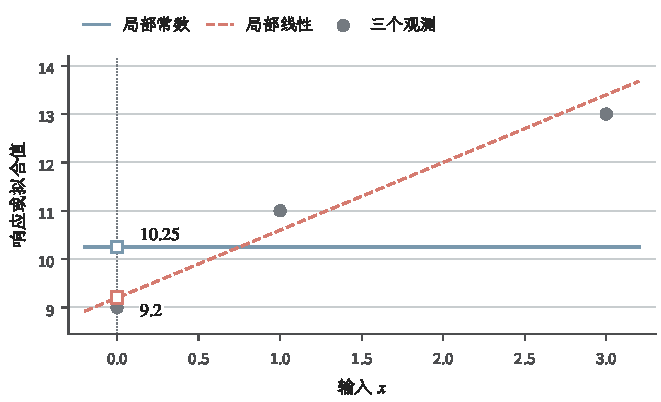
\includegraphics[width=\linewidth]{figures/math-preparation/concept-revision-probability/statistics-local-boundary-fit.pdf}
  \caption{边界处的局部常数与局部线性拟合（教学数据图）。观测为\((0,9),(1,11),(3,13)\)，权重为\(1,0.75,0.25\)。蓝实线为加权常数\(10.25\)，红虚线为\(9.2+1.4x\)，边界\(x_0=0\)处分别预测\(10.25\)和\(9.2\)。}
  \label{fig:statistics-local-boundary-fit}
\end{figure}

在上述独立同分布抽样下，这些方法的一致性需要邻域既缩小又包含越来越多样本。
例如一维内部点处，若输入密度在
\(x\)附近连续且为正，条件均值足够光滑，条件方差局部有界，并取
\(h\to0\)、\(nh\to\infty\)，局部常数估计的平滑偏差消失，局部平均的方差也消失。
输入密度与条件均值都二阶连续可微时，常用局部展开给出\(O(h^2)\)的平滑偏差
以及\(O((nh)^{-1})\)的方差，因此平滑偏差的平方为\(O(h^4)\)；精确常数还依赖
核、输入密度与条件噪声。近邻版本相应要求\(k\to\infty\)且\(k/n\to0\)。
这些都是目标分布有局部覆盖时的内插结论；在训练输入密度为零的区域，缩小邻域无法产生
新信息，外推保证必须来自额外结构假设。

\section{模型比较与数据获取}
\label{sec:stats-model-comparison-data-acquisition}

当一个模型或一批数据不足以回答问题时，有两种决策需要区分：用现有数据比较候选模型，
以及通过新的对照或观测增加信息。模型证据需要统一比较口径；实验设计需要说明新增数据
将减少哪一项不确定性。二者都使用前面的推断工具，却改变不同的决策对象。

\subsection{模型证据与局部积分近似}
\label{sec:statistics-model-evidence}

上一组工具评价预测分布；多个模型竞争时，还需先决定比较的是训练拟合、未来预测还是模型证据。
边缘似然对参数积分，Laplace近似用局部曲率近似这项积分。
信息准则的惩罚形式虽可能相似，比较目标和渐近条件却不同。

\subsubsection{预测、似然与边缘似然}

模型选择准则并非都在回答同一问题。独立测试误差比较未来预测；训练似然衡量已观测数据
在拟合参数下的密度；边缘似然
\[
  p(\bm y\mid M)
  =\int p(\bm y\mid\vartheta,M)\pi(\vartheta\mid M)\,\mathrm d\vartheta
\]
对参数不确定性积分；编码长度则把模型和数据的描述代价相加。一个模型可能训练似然高，
却因复杂度、先验体积或泛化误差而不被其他准则选择。

\begin{definition}[Bayes因子]
  \label{def:statistics-bayes-factor}
两个模型\(M_1,M_0\)的\term{Bayes因子}（Bayes factor）是
\[
  \operatorname{BF}_{1,0}
  =\frac{p(\bm y\mid M_1)}{p(\bm y\mid M_0)}.
\]
这里两个边缘似然都由概率先验得到；所比较的数据处，分母严格为正且有限，分子有限且可为零。
\end{definition}
Bayes因子更新的是模型间先验赔率，
不是与先验无关的“模型为真概率”。在高斯位置模型中，若
\(\theta\sim\mathcal N(0,A^2)\)，则
\(\overline Y\sim\mathcal N(0,A^2+\sigma^2/n)\)。保持似然峰值不变而增大\(A\)
会把先验质量摊到更宽区域；对固定\(\overline y\)，当\(A\to\infty\)时该边缘密度
趋于零。这正是模型证据依赖参数先验尺度的一个可复核例子。

\subsubsection{Laplace近似与BIC}

\begin{theorem}[固定维Laplace局部积分近似]
\label{thm:statistics-laplace-approximation}
设\(\Theta\subseteq\mathbb{R}^d\)为可测集，
\(\widehat{\bm\vartheta}\in\operatorname{int}(\Theta)\)。函数
\(h:\Theta\to\mathbb{R}\)可测，并在
\(\widehat{\bm\vartheta}\)的某个邻域内二阶连续可微；该点是\(h\)在\(\Theta\)上的
唯一全局最大点，且
\(\bm H=-\nabla^2h(\widehat{\bm\vartheta})\)正定。函数
\(g:\Theta\to[0,\infty)\)局部可积，在该点的某个邻域内连续，并满足
\(g(\widehat{\bm\vartheta})>0\)。

进一步假设存在\(\delta,\eta>0\)和\(n_0\geq1\)，使
\(\overline{B_\delta(\widehat{\bm\vartheta})}\subseteq\Theta\)，\(h,g\)在该闭球
所在的邻域内分别满足上述光滑性与连续性，并且
\[
  \sup_{\bm\vartheta\in
    \Theta\setminus B_\delta(\widehat{\bm\vartheta})}
  h(\bm\vartheta)
  \leq h(\widehat{\bm\vartheta})-\eta,
  \qquad
  \int_\Theta
  \exp\!\left\{n_0\bigl[h(\bm\vartheta)
    -h(\widehat{\bm\vartheta})\bigr]\right\}
  g(\bm\vartheta)\,\mathrm d\bm\vartheta<\infty.
\]
则当\(n\to\infty\)时，
\[
  \int_\Theta \exp\{n h(\bm\vartheta)\}g(\bm\vartheta)\,
  \mathrm d\bm\vartheta
  =
  \exp\{nh(\widehat{\bm\vartheta})\}
  g(\widehat{\bm\vartheta})
  \left(\frac{2\pi}{n}\right)^{d/2}
  |\bm H|^{-1/2}\{1+o(1)\}.
\]
\end{theorem}

\begin{proof}
正定性与二阶连续性保证：必要时缩小\(\delta\)，存在\(c>0\)，使闭球内有
\[
  h(\bm\vartheta)-h(\widehat{\bm\vartheta})
  \leq-c\lVert\bm\vartheta-\widehat{\bm\vartheta}\rVert_2^2.
\]
缩小闭球后，原闭球中剩余的紧致环带由唯一最大性给出严格间隔；把它与原来的尾部间隔
合并，仍可取某个\(\eta>0\)满足定理中的一致上界。另一方面，在最大点附近作多元
Taylor展开：
\[
  h(\bm\vartheta)
  =
  h(\widehat{\bm\vartheta})
  -\frac12(\bm\vartheta-\widehat{\bm\vartheta})^\top
  \bm H(\bm\vartheta-\widehat{\bm\vartheta})
  +o(\lVert\bm\vartheta-\widehat{\bm\vartheta}\rVert_2^2).
\]
令
\(\bm u=\sqrt n\,\bm H^{1/2}
(\bm\vartheta-\widehat{\bm\vartheta})\)，则逆变换的Jacobian行列式绝对值为
\(n^{-d/2}|\bm H|^{-1/2}\)，即
\(\mathrm d\bm\vartheta
=n^{-d/2}|\bm H|^{-1/2}\mathrm d\bm u\)。对每个固定的\(\bm u\)，
Taylor展开与\(g\)的连续性
使变换后的被积函数收敛到
\(g(\widehat{\bm\vartheta})\exp(-\lVert\bm u\rVert_2^2/2)\)。局部二次上界和
\(g\)在闭球上的有界性给出可积的高斯控制函数，因此支配收敛定理给出
\[
  \int_{B_\delta(\widehat{\bm\vartheta})}
  \exp\!\left\{n\bigl[h(\bm\vartheta)
    -h(\widehat{\bm\vartheta})\bigr]\right\}
  g(\bm\vartheta)\,\mathrm d\bm\vartheta
  =
  n^{-d/2}|\bm H|^{-1/2}
  g(\widehat{\bm\vartheta})(2\pi)^{d/2}\{1+o(1)\}.
\]
闭球外的尾项满足
\[
  \int_{\Theta\setminus B_\delta(\widehat{\bm\vartheta})}
  e^{n[h(\bm\vartheta)-h(\widehat{\bm\vartheta})]}
  g(\bm\vartheta)\,\mathrm d\bm\vartheta
  \leq
  e^{-(n-n_0)\eta}
  \int_\Theta
  e^{n_0[h(\bm\vartheta)-h(\widehat{\bm\vartheta})]}
  g(\bm\vartheta)\,\mathrm d\bm\vartheta
  =o(n^{-d/2}).
\]
局部主项与该尾项相加即得结论。
\end{proof}

上一定理描述固定函数\(h\)的基本形式。在正则独立样本模型中，实际处理的是随机函数
序列
\[
  nh_n(\bm\vartheta)=\ell_n(\bm\vartheta)
  =\sum_{i=1}^n\log p_\vartheta(y_i),\qquad
  g(\bm\vartheta)=\pi(\bm\vartheta).
\]
若极大似然估计以内点唯一最大点的形式收敛，归一化观测信息矩阵收敛到正定极限，先验
在极限点附近连续且为正，并且局部二次展开与尾部控制对该序列一致成立，则相同论证给出
\[
  \log p(\bm y\mid M)
  =
  \ell_n(\widehat{\bm\vartheta})
  -\frac d2\log n+O_{\mathbb{P}}(1).
\]
对固定的有限候选模型集合，乘以\(-2\)并只保留随\(n\)发散的项，得到常用形式
\[
  \operatorname{BIC}
  =-2\ell_n(\widehat{\bm\vartheta})+d\log n.
\]
惩罚来自后验高密度区域体积随\(n^{-d/2}\)缩小，而不是人为给参数个数加价。

\subsubsection{AIC、描述长度与比较口径}

在独立、固定维且正则的最大似然设定中，常用
\[
  \operatorname{AIC}
  =-2\ell_n(\widehat{\bm\vartheta})+2d.
\]
其中\(2d\)是一阶校正拟合对预期样本外对数损失的乐观偏差，目标是预测失配；模型失配
时还要核对适用的协方差校正，不能只数参数。BIC近似特定先验下的边缘似然，常以候选中
存在真模型的正则渐近为背景。\term{最小描述长度}（minimum description length,
MDL）则先规定可解码的模型代码与给定模型后的数据代码，再最小化二者总长度；更换编码
对象或精度约定会改变有限样本准则。三者惩罚形式相似时也不能互换解释，更不能共享未经
证明的选择一致性。

混合模型的标签交换、参数位于边界、额外成分权重为零或Fisher信息奇异时，最大点可能
不唯一，局部曲率可能退化，常规Laplace展开和\(d\log n\)惩罚随之失效。此时应使用
适合奇异模型的方法、数值积分或明确的近似；近似边缘似然不能写成精确证据。

\subsection{对照、预算与信息获取}
\label{sec:statistics-design-information}

\subsubsection{随机分配与可复核对照}

推断质量不仅由分析方法决定，也由数据如何取得决定。每个对象在各处理下本会产生的结果
称为潜在结果，正式的因果目标将在第~\ref{chap:causal-inference}章定义。随机分配使
处理指派在设计上独立于这些预先固定的结果，从而把系统差异转成可量化的随机误差。
配对对照先按对象或关键协变量配对，
再在对内比较，可消除共享噪声。若配对质量差或分析时忽略配对，预期的方差收益不会自动
出现。

先看最简单的两组位置模型。若随机分配后两组分别有\(n_A,n_B\)个独立观测，均值为
\(\mu_A,\mu_B\)，方差为\(\sigma_A^2,\sigma_B^2\)，则
\[
  \widehat\Delta=\overline Y_A-\overline Y_B,\qquad
  \mathbb{E}[\widehat\Delta]=\mu_A-\mu_B,
\]
\[
  \operatorname{Var}(\widehat\Delta)
  =\frac{\sigma_A^2}{n_A}+\frac{\sigma_B^2}{n_B}.
\]
随机化建立的是处理指派与处理前对象特征之间的概率关系，并不要求两种处理下的结果
服从同一分布。上式还假设组间独立且组内方差有限；配对随机化应改为分析对内差值。
它提供的是设计下的可复核比较，潜在结果目标及从试验人群向目标总体的推广条件由
第~\ref{chap:causal-inference}章继续建立。

消融实验删除一个组件并保持其他条件不变，用来判断该组件对整体结果的增量贡献。它不能
在组件强交互时给出唯一的“独立贡献”，也不能用不同训练预算的两个系统冒充单因素比较。
基线、随机种子、停止规则和评价集都应在比较前固定。

学习曲线把训练样本量或计算量与验证性能联系起来。只报告最终点无法区分方法是数据效率
更高，还是只是使用了更多数据和算力。实验至少要区分数据预算、计算预算与评价时间预算：
收集更多标签、搜索更多配置和反复占用测试集是三种不同资源。

\subsubsection{预算下的精度与信息价值}

预算分配应对应希望降低的误差。若两组单位观测成本相同且
\(n_A+n_B=N\)，最小化上面的均值差方差可得
\[
  \frac{n_A}{n_B}=\frac{\sigma_A}{\sigma_B}.
\]
这是对\(n_A\)求导或用Cauchy--Schwarz得到的Neyman分配：波动较大的组需要更多
观测。方差未知时要用先验信息或先导样本估计，估计误差也应计入设计；整数、最低组规模
和不同成本会改变解。

线性观测模型
\(\bm y=\bm X\bm\beta+\bm\varepsilon\)提供了多方向设计的接口，其中
\(\bm X\in\mathbb{R}^{n\times d}\)、\(\bm\beta,\bm a\in\mathbb{R}^d\)。
给定满列秩设计矩阵\(\bm X\)，假设
\(\mathbb{E}[\bm\varepsilon\mid\bm X]=\bm{0}\)且
\(\operatorname{Cov}(\bm\varepsilon\mid\bm X)=\sigma^2\bm I_n\)。
普通最小二乘估计量为
\[
  \widehat{\bm\beta}
  =(\bm X^\top\bm X)^{-1}\bm X^\top\bm y.
\]
它在给定\(\bm X\)时无偏，并且
\[
  \operatorname{Var}(\bm a^\top\widehat{\bm\beta}\mid\bm X)
  =\sigma^2\bm a^\top(\bm X^\top\bm X)^{-1}\bm a.
\]
因此新增观测的特征方向会改变设计矩阵，并降低某些\(\bm a\)方向的方差；它未必同样
改善其他方向、预测总体或非线性目标。最小化最坏方向、平均方向或行列式体积会得到不同
设计准则，必须先声明评价对象。

当标注预算有限时，\term{主动学习}（active learning）根据当前模型选择下一批待标注
样本。若效用\(U\)已经包含任务收益与查询成本，一个理想选择可写成最大化期望效用增量：
\[
  x^\star\in\argmax_x
  \mathbb{E}_{Y\mid x,\mathcal D}
  \left[
    U(\mathcal D\cup\{(x,Y)\})-U(\mathcal D)
  \right],
\]
其中\(U\)衡量后验不确定性减少或决策效用增加。只选当前最不确定样本是一种替代规则，
不一定等于任务价值最大。若把效用设为后验熵的负值，\(U(\mathcal D)=-H(\Theta\mid\mathcal D)\)，则期望效用增量就是预期熵下降，才与
第~\ref{chap:information-theory-and-statistical-geometry}章的互信息接口相连；若
\(U\)取行动后的最优风险，则接到第~\ref{sec:decision-value-of-information}节的
信息价值。信息量增加与任务效用增加不是同一命题。

主动选择会改变被标注样本的分布。若候选池不覆盖目标总体，算法无法询问缺失区域；
若标注噪声随难度变化，不确定样本还可能最不可靠；若最终指标用同一批自适应选择数据
计算，评价也会偏移。因此应在比较前固定可访问数据、查询成本、标注机制和独立评价集。
查询依赖过去答案时，所选特征或对象必须在新噪声揭示前由历史信息确定，才能回用
第~\ref{chap:stochastic-processes-and-approximation}章的可预测设计与自适应误差工具；
把自适应记录事后当作固定独立样本没有同样保证。
实验设计不是分析完成后的附注，而是可识别性和误差保证的一部分。

\section{本章小结}
\label{sec:statistics-summary}

带噪观测不能单靠样本量变成可靠结论。统计推断先确定目标总体和抽样单位，再检查未知
目标能否由观测分布识别。似然、矩条件和稳健准则提供不同的估计途径；偏差、方差、
Fisher信息与渐近分布说明它们在正则条件下能达到什么精度。在线性均值模型中，Gauss--Markov
定理给出同方差不相关噪声下的有限样本效率比较，但范围限于线性无偏估计。Bayes更新把先验假设纳入
同一计算，并通过后验预测保留参数与未来噪声两层不确定性。

点估计、置信区间、可信区间、预测区间和检验各有不同的随机对象，不能因数值形式相近
而混用。重采样必须尊重独立单位，多重选择和持续查看必须进入误差控制。概率评分评价
整个预测分布，校准、区分能力与锐度分别检查不同性质；非参数平滑放宽分布形状假设，缺失机制则决定未见部分能否由已见数据恢复；二者分别处理模型表示与信息缺口。

模型证据依赖选择目标和正则条件，Laplace近似、BIC、AIC与编码长度不提供无条件一致的
答案。最终，随机对照、预算安排和主动获取决定了数据中能够出现什么信息。
第~\ref{chap:information-theory-and-statistical-geometry}章将从信息量与可区分性研究
推断的根本限制，第~\ref{chap:causal-inference}章则在干预目标下重新检查“观测到的
关联能否识别行动效果”。

\chapter{信息论与统计几何}
\label{chap:information-theory-and-statistical-geometry}
概率论给出了分布、条件化和换测度的语言，数理统计则把未知分布或参数作为推断对象。
不过，仅仅知道两个模型的参数相差多少，还不能判断观测能否区分它们。对
\(\mathcal{N}(0,1)\)与\(\mathcal{N}(0.1,1)\)，均值差、对数似然差、事件概率差
和搬运质量所需的距离都可以计算，但它们回答的是不同问题；若把均值重新参数化为其
立方根，参数的欧氏距离还会随坐标改变。
本章研究怎样从分布本身比较不确定性、可区分性与局部变化。编码长度引出熵，预测分布
的对数损失引出相对熵；事件、测试函数和搬运成本又给出不同的分布差异。换测度的指数
矩不等式把这些差异接到学习保证，Le Cam与Fano方法则把“分布太相近”转成任何估计器
都无法越过的误差下界。在几何一侧，Wasserstein距离从质量搬运刻画全局位置变化，Fisher度量
从KL的二阶项刻画参数模型的局部几何，变分表达把推断与分布优化连接起来。
除非另有说明，本章使用自然对数，信息量的单位为nat。若改用以\(2\)为底的对数，信息
量单位为bit，所有数值只相差常数因子。第~\ref{chap:probability-theory}章已经建立
Radon--Nikodym导数、条件分布与指数族；本章在使用这些对象时仍逐项核对绝对连续、
可积性和正则性。
\section{不确定性与熵}
\label{sec:information-entropy}
\subsection{平均编码长度为何出现对数}
设离散随机变量\(X\)取值于有限或可数字母表\(\mathcal{X}\)，质量函数为\(p(x)\)。
若使用二进制前缀码，结果\(x\)的码长记为\(\ell(x)\)。前缀码的码字不能是另一
码字的前缀，因而码长必须满足Kraft不等式
\[
  \sum_{x\in\mathcal{X}}2^{-\ell(x)}\leq1.
\]
概率较大的结果应分配较短码字，但码长不能彼此独立地任意缩短。理想实数码长
\(-\log_2p(x)\)恰好满足等号，因为\(\sum_xp(x)=1\)。
\begin{definition}[离散熵]
\label{def:information-discrete-entropy}
若\(\sum_xp(x)|\log p(x)|<\infty\)，则\(X\)的\term{熵}（entropy）定义为
\begin{equation}
  H(X)
  =
  -\sum_{x\in\mathcal{X}}p(x)\log p(x)
  =
  \mathbb{E}[-\log p(X)],
  \label{eq:information-discrete-entropy}
\end{equation}
其中约定\(0\log0=0\)。
\end{definition}
熵是按真实发生频率加权的理想描述长度。它不是某次结果携带的信息，而是结果发生前的
平均不确定性。若\(X\)几乎必然为常数，则\(H(X)=0\)；若\(X\)在\(m\)个结果上均匀
分布，则\(H(X)=\log m\)\scite{math-cover2006information}
例如，若\(X\sim\operatorname{Bernoulli}(1/4)\)，则
\[
  H(X)
  =
  -\frac14\log\frac14-\frac34\log\frac34
  \approx0.5623\ \text{nat}
  \approx0.8113\ \text{bit}.
\]
二元前缀码必须给两个结果各分配至少一位，所以其逐符号平均码长为\(1\) bit；熵给出
理想实数码长的平均值，二者的差来自整数码长约束。
\begin{theorem}[无失真前缀码的平均长度界]
\label{thm:information-source-coding-bound}
对熵有限的质量函数\(p\)和任意满足Kraft不等式的二进制码长\(\ell(x)\)，有
\[
  \mathbb{E}[\ell(X)]\geq H(X)/\log2.
\]
反过来，在有效字母表
\(\mathcal X_+=\{x:p(x)>0\}\)上取
\(\ell(x)=\lceil-\log_2p(x)\rceil\)，可构造前缀码，并满足
\[
  \mathbb{E}[\ell(X)]<H(X)/\log2+1.
\]
\end{theorem}
\begin{proof}
令\(K=\sum_x2^{-\ell(x)}\leq1\)，并在\(K>0\)时定义
\(q(x)=2^{-\ell(x)}/K\)。由\(-\log u\geq1-u\)，
\(\sum_xp(x)\log[p(x)/q(x)]\geq
1-\sum_{x:p(x)>0}q(x)\geq0\)，因此
\[
  0\leq\sum_xp(x)\log\frac{p(x)}{q(x)}
  =
  -H(X)+(\log2)\mathbb{E}[\ell(X)]+\log K.
\]
由于\(\log K\leq0\)，移项便得到下界。对取整码长，
\(2^{-\ell(x)}\leq p(x)\)，故Kraft不等式成立。为看清逆向构造，按码长从短到长排列
\(\mathcal X_+\)，依次在\([0,1)\)中放置长度为\(2^{-\ell(x)}\)且端点与该层二进
网格对齐的区间；Kraft不等式保证所有区间都能放下。用每个区间左端点的前
\(\ell(x)\)个二进制位作为码字。两个这样的二进区间若相交，较短码字必为较长码字的
前缀；构造中的区间互不相交，所以所得码是前缀码。这就是Kraft--McMillan逆向构造。
又因\(\lceil a\rceil<a+1\)，对\(p(x)>0\)逐项平均即得上界。满足\(p(x)=0\)的符号
不会由信源产生，对熵和平均码长均无贡献，因而从有效字母表中删除；若应用要求传输这些
符号，必须另外为它们保留码空间，相应冗余不由上述小于一位的界保证。
\end{proof}
这个结论只讨论无失真、逐符号可唯一解析的编码。允许块编码时，每个符号的整数取整代价
可以趋近于零；允许失真时，最优码长还取决于失真准则，不能只由\(H(X)\)决定。
\subsection{条件熵与链式法则}
对离散随机变量\(X,Y\)，给定\(Y=y\)后仍需描述\(X\)的平均长度为
\[
  H(X\mid Y=y)
  =
  -\sum_xp(x\mid y)\log p(x\mid y).
\]
再对\(Y\)平均，得到\term{条件熵}（conditional entropy）
\begin{equation}
  H(X\mid Y)
  =
  -\sum_{x,y}p(x,y)\log p(x\mid y).
  \label{eq:information-conditional-entropy}
\end{equation}
它衡量已经知道\(Y\)以后，\(X\)还剩多少不确定性。
对可数字母表，这个定义允许取值\(+\infty\)。以下推导假设
\(H(X,Y)<\infty\)，从而出现的边缘熵与条件熵均为有限值。此时
联合质量分解为\(p(x,y)=p(y)p(x\mid y)\)，所以
\[
\begin{aligned}
  H(X,Y)
  &=
  -\sum_{x,y}p(x,y)\log p(x,y)\\
  &=
  -\sum_{x,y}p(x,y)\log p(y)
  -\sum_{x,y}p(x,y)\log p(x\mid y)\\
  &=
  H(Y)+H(X\mid Y).
\end{aligned}
\]
这就是熵的链式法则。反复使用可得
\begin{equation}
  H(X_1,\ldots,X_n)
  =
  \sum_{i=1}^{n}H(X_i\mid X_1,\ldots,X_{i-1}).
  \label{eq:information-entropy-chain-rule}
\end{equation}
其中假设\(H(X_1,\ldots,X_n)<\infty\)。链式法则是同一联合分布的不同分解，
不要求变量独立。若允许扩展值，同一等式仍可由非负项求和得到，但不能把它改写成
两个无穷熵之差。
\subsection{互信息衡量观察带来的减少量}
\begin{definition}[互信息与条件互信息]
\label{def:information-mutual-information}
离散变量\(X,Y\)的\term{互信息}（mutual information, MI）定义为
\begin{equation}
  I(X;Y)
  =
  \sum_{x,y}p(x,y)
  \log\frac{p(x,y)}{p(x)p(y)}.
  \label{eq:information-mutual-information}
\end{equation}
其中\(p(x,y)=0\)的项约定为零；该对数比求和允许取值\(+\infty\)，但不拆成两个
可能无穷的熵之差。它比较实际联合质量\(p(x,y)\)与独立情形下的乘积质量
\(p(x)p(y)\)。
给定\(Z\)后的\term{条件互信息}定义为先固定\(Z=z\)计算同一对数比，再对\(Z\)平均：
\begin{equation}
  I(X;Y\mid Z)
  =
  \sum_{z:p(z)>0}p(z)
  \sum_{x,y}p(x,y\mid z)
  \log
  \frac{p(x,y\mid z)}
       {p(x\mid z)p(y\mid z)}.
  \label{eq:information-conditional-mutual-information}
\end{equation}
\end{definition}
上述定义不涉及无穷量相减。若\(H(X,Y)<\infty\)，利用熵的链式法则可进一步写成
\begin{equation}
  I(X;Y)
  =
  H(X)-H(X\mid Y)
  =
  H(Y)-H(Y\mid X).
  \label{eq:information-mi-entropy-reduction}
\end{equation}
因此它可以解释为观察一个变量后另一个变量平均减少的不确定性。条件互信息则先固定
已有信息\(Z\)，再衡量\(Y\)还能为\(X\)提供多少信息。对每个\(z\)，对数和不等式
保证内层求和非负，所以条件互信息也非负，并且可能为\(+\infty\)；在可数离散情形中，
它等于零当且仅当
\(X\perp Y\mid Z\)几乎处处成立。
\begin{theorem}[数据处理不等式]
\label{thm:information-data-processing}
若离散随机变量满足Markov关系\(X\to Y\to Z\)，即
\(X\perp Z\mid Y\)，并且相关互信息有限，则
\[
  I(X;Z)\leq I(X;Y).
\]
\end{theorem}
\begin{proof}
对同一个联合分布按两种顺序使用互信息链式法则，有
\[
\begin{aligned}
  I(X;Y,Z)
  &=I(X;Y)+I(X;Z\mid Y)=I(X;Y),\\
  I(X;Y,Z)
  &=I(X;Z)+I(X;Y\mid Z)\geq I(X;Z).
\end{aligned}
\]
第一行使用Markov关系，第二行使用条件互信息非负性。合并两式即得结论。
\end{proof}
这里的“处理”可以是确定映射，也可以是仅依赖\(Y\)的随机通道。结论说明后处理不能
凭空增加关于\(X\)的信息，但不保证任意特定任务的误差严格变差；若处理丢弃的方向与
任务无关，等号仍可能成立。一般可测空间上的版本不能依赖离散求和；下一节正式定义
KL后，将用KL的数据处理性质回收这一表达，避免有限熵中的无穷量相减。
\begin{example}[一次带噪二元观测]
\label{ex:information-binary-channel}
令\(X\)在\(\{0,1\}\)上均匀分布，观测\(Y=X\oplus N\)，其中
\(N\sim\operatorname{Bernoulli}(\varepsilon)\)与\(X\)独立，
\(0\leq\varepsilon\leq1/2\)。由于\(Y\)也均匀，
\[
  H(X)=\log2,\qquad
  H(X\mid Y)=
  -\varepsilon\log\varepsilon
  -(1-\varepsilon)\log(1-\varepsilon).
\]
记二元熵函数为
\[
  H_{\mathrm{b}}(u)
  =
  -u\log u-(1-u)\log(1-u),
  \qquad 0\leq u\leq1,
\]
其中沿用\(0\log0=0\)的约定。所以
\[
  I(X;Y)=\log2-H_{\mathrm{b}}(\varepsilon).
\]
当\(\varepsilon=0\)时，观测完整揭示\(X\)；当\(\varepsilon=1/2\)时，观测与
\(X\)独立，互信息为零。该数值描述平均可辨识信息，不保证每次观测都恢复正确。
\end{example}
\subsection{微分熵依赖坐标}
若连续随机向量\(\bm{X}\in\mathbb{R}^d\)具有密度\(p\)，并且
\(\mathbb{E}|\log p(\bm{X})|<\infty\)，定义
\term{微分熵}（differential entropy）
\[
  h(\bm{X})
  =
  -\int p(\bm{x})\log p(\bm{x})\,\mathrm{d}\bm{x}.
\]
它可以为负，也不具有离散熵“至少为零”的性质。设
\(g:\mathbb{R}^d\to\mathbb{R}^d\)是满足第~\ref{chap:probability-theory}章
密度换元定理条件的\(C^1\)微分同胚，并且
\[
  \mathbb{E}\!\left[
    \left|\log\left|\det\bm{J}_g(\bm{X})\right|\right|
  \right]
  <\infty.
\]
此时\(\bm{Y}=g(\bm{X})\)仍有密度，换元公式给出
\begin{equation}
  h(\bm{Y})
  =
  h(\bm{X})
  +
  \mathbb{E}\!\left[
    \log\left|\det\bm{J}_{g}(\bm{X})\right|
  \right].
  \label{eq:information-differential-entropy-transform}
\end{equation}
特别地，\(Y=aX\)时\(h(Y)=h(X)+\log|a|\)。坐标单位从米改成厘米就会改变微分熵，
所以不能把它单独当成坐标不变的分布差异。互信息和KL中的Jacobian矩阵项会相消，在适当
可逆变换下保持不变。
更一般地，若\(\bm{Y}=\bm{A}\bm{X}+\bm{b}\)，其中
\(\bm{A}\in\mathbb{R}^{d\times d}\)可逆，且相关积分有限，则
\[
  h(\bm{Y})=h(\bm{X})+\log|\det\bm{A}|.
\]
微分熵为负并不矛盾。例如\(X\)在区间\([0,1/2]\)上均匀分布时，密度为\(2\)，故
\(h(X)=-\log2\)。这反映密度值依赖坐标尺度，而不是出现了“负的不确定性”。
\section{预测分布与对数评分}
\label{sec:information-log-score-kl}
\subsection{交叉熵把预测质量写成平均损失}
真实分布为\(P\)，预测分布为\(Q\)。若二者在离散空间上的质量分别为\(p,q\)，观察
\(X\sim P\)后给预测者的\term{对数损失}为\(-\log q(X)\)。其平均值
\begin{equation}
  H(P,Q)
  =
  -\sum_xp(x)\log q(x)
  \label{eq:information-cross-entropy}
\end{equation}
称为\term{交叉熵}（cross-entropy）。它不是\(Q\)自身的不确定性，而是用\(Q\)
描述来自\(P\)的结果时付出的平均代价。
\begin{definition}[相对熵]
\label{def:information-kl-divergence}
同一可测空间上的概率测度\(P,Q\)若满足\(P\ll Q\)，则
\term{相对熵}（relative entropy），也称KL散度，定义为
\begin{equation}
  D_{\mathrm{KL}}(P\Vert Q)
  =
  \int\log\frac{\mathrm{d}P}{\mathrm{d}Q}\,\mathrm{d}P.
  \label{eq:information-kl-divergence}
\end{equation}
若\(P\not\ll Q\)，约定\(D_{\mathrm{KL}}(P\Vert Q)=+\infty\)。
\end{definition}
由这个定义，式~\eqref{eq:information-mutual-information}可简写为
\[
  I(X;Y)
  =
  D_{\mathrm{KL}}(P_{XY}\Vert P_X\otimes P_Y),
\]
条件互信息则是条件联合分布与条件边缘乘积分布之间KL的平均。这也把前一节的离散求和
推广到允许正则条件分布的一般可测空间。
在离散情形中，
\[
  D_{\mathrm{KL}}(P\Vert Q)
  =
  \sum_xp(x)\log\frac{p(x)}{q(x)},
\]
并且
\begin{equation}
  H(P,Q)=H(P)+D_{\mathrm{KL}}(P\Vert Q).
  \label{eq:information-cross-entropy-decomposition}
\end{equation}
真实分布固定时，最小化交叉熵等价于最小化从\(P\)到\(Q\)的KL散度。
以二值结果为例，取\(P=\operatorname{Bernoulli}(0.9)\)和
\(Q=\operatorname{Bernoulli}(0.6)\)，则
\[
\begin{aligned}
  D_{\mathrm{KL}}(P\Vert Q)&\approx0.2263,\\
  D_{\mathrm{KL}}(Q\Vert P)&\approx0.3112.
\end{aligned}
\]
两个方向使用不同分布作平均，因而数值不同。若预测分布把结果\(1\)的概率改为零，而
真实分布仍给该结果正概率，则前向交叉熵与KL都变为无穷。
\subsection{Gibbs不等式与严格适当性}
\begin{theorem}[Gibbs不等式]
\label{thm:information-gibbs-inequality}
任意概率测度\(P,Q\)满足
\[
  D_{\mathrm{KL}}(P\Vert Q)\geq0,
\]
且在散度有限时，等号成立当且仅当\(P=Q\)。
\end{theorem}
\begin{proof}
只需处理\(P\ll Q\)的情形。以\(\mu=P+Q\)为共同支配测度，密度记为\(p,q\)，
并在\(\{p>0\}\)上令\(r=q/p\)。由\(-\log u\geq1-u\)，
\[
  D_{\mathrm{KL}}(P\Vert Q)
  =
  \mathbb{E}_P[-\log r]
  \geq
  1-\mathbb{E}_P[r].
\]
若\(Q\)还在\(P\)的零集上放有质量，则
\(\mathbb{E}_P[r]\leq1\)；故右侧非负。等号要求
\(-\log r=1-r\)在\(P\)-几乎处处成立，也就是\(r=1\)，同时\(Q\)不能在
\(P\)的零集上留下额外质量。因此\(P=Q\)。
\end{proof}
式~\eqref{eq:information-cross-entropy-decomposition}与Gibbs不等式说明，对数
评分在真实分布处取得唯一最小期望损失，因而是严格适当评分规则。这是一项总体期望
性质：有限样本经验交叉熵最低的模型未必最接近真实分布，模型族限制、优化误差和样本
误差仍需分别处理。
对一般随机元素，互信息仍按
\[
  I(X;Y)=D_{\mathrm{KL}}(P_{XY}\Vert P_X\otimes P_Y)
\]
定义，条件互信息则是正则条件分布之间KL的平均；这要求所在空间允许选取相应条件分布。
Gibbs不等式立即给出非负性，并且零值分别等价于联合分布等于边缘乘积、条件联合分布
几乎处处等于条件边缘乘积。KL链式法则还给出
\[
  I(X;Y,Z)=I(X;Y)+I(X;Z\mid Y),
\]
只要相关正则条件分布存在；用扩展值形式陈述时不需要把互信息写成可能未定义的熵之差。
\subsection{方向、支持与同一高斯位置族}
KL散度通常不对称。若\(P\)在某区域有正质量而\(Q\)给出零质量，则
\(D_{\mathrm{KL}}(P\Vert Q)=+\infty\)；反向散度是否有限取决于反向支持关系。
即使两个方向都有限，数值也通常不同。因此“最小化KL”必须说明哪个分布位于前面。
KL也不满足三角不等式。令\(P,Q,R\)依次为参数\(0.1,0.2,0.3\)的Bernoulli分布，
可算得
\[
  D_{\mathrm{KL}}(P\Vert R)\approx0.1163
  >
  D_{\mathrm{KL}}(P\Vert Q)+D_{\mathrm{KL}}(Q\Vert R)
  \approx0.0624.
\]
对具有相同方差\(\sigma^2>0\)的高斯位置族
\[
  P=\mathcal{N}(\mu,\sigma^2),
  \qquad
  Q=\mathcal{N}(\nu,\sigma^2),
\]
直接代入密度比可得
\begin{equation}
  D_{\mathrm{KL}}(P\Vert Q)
  =
  \frac{(\mu-\nu)^2}{2\sigma^2}.
  \label{eq:information-gaussian-location-kl}
\end{equation}
同一计算可直接推广到向量平移。若
\[
  P=\mathcal{N}(\bm{\mu},\bm{\Sigma}),\qquad
  Q=\mathcal{N}(\bm{\nu},\bm{\Sigma}),
\]
其中\(\bm{\mu},\bm{\nu}\in\mathbb{R}^d\)，共同协方差
\(\bm{\Sigma}\in\mathbb{R}^{d\times d}\)对称正定，则
\begin{equation}
  D_{\mathrm{KL}}(P\Vert Q)
  =
  \frac12
  (\bm{\mu}-\bm{\nu})^{\top}
  \bm{\Sigma}^{-1}
  (\bm{\mu}-\bm{\nu}).
  \label{eq:information-vector-gaussian-translation-kl}
\end{equation}
这里比较的是白化后的均值位移：沿低方差方向移动相同欧氏距离更容易被观测区分。若共同
协方差只半正定，则还要检查两分布是否位于同一仿射支持上；均值差不在
\(\operatorname{range}(\bm{\Sigma})\)中时KL为无穷，不能直接把逆矩阵替换成伪逆而
省略支持条件。标量或向量公式的对称性都来自共同协方差，并不代表一般KL具有对称性。
\subsection{约束下的最大熵分布}
只给出若干矩约束时，可能有许多分布与已知信息相容。\term{最大熵原理}选择其中熵最大
者，即不额外加入约束未提供的集中结构。设参考测度为\(\mu\)，要求密度\(p\)满足
\[
  \int p\,\mathrm{d}\mu=1,
  \qquad
  \int T_jp\,\mathrm{d}\mu=\tau_j,
  \quad j=1,\ldots,k.
\]
若存在参数\(\bm{\lambda}\)使
\[
  p_{\bm{\lambda}}(x)
  =
  \exp\left\{
    \bm{\lambda}^{\top}\bm{T}(x)
    -A(\bm{\lambda})
  \right\}
\]
满足这些约束，其中
\(A(\bm{\lambda})=\log\int
e^{\bm{\lambda}^{\top}\bm{T}(x)}\,\mathrm{d}\mu(x)<\infty\)，则对任意同样可行的
密度\(p\)，
\[
\begin{aligned}
  D_{\mathrm{KL}}(p\Vert p_{\bm{\lambda}})
  &=
  \int p\log p\,\mathrm{d}\mu
  -\bm{\lambda}^{\top}\bm{\tau}
  +A(\bm{\lambda})\\
  &=
  -h(p)+h(p_{\bm{\lambda}})\geq0.
\end{aligned}
\]
所以\(p_{\bm{\lambda}}\)最大化熵，且在几乎处处意义下唯一。该结论要求可行分布和
归一化常数存在，也要求相关积分有限。矩约束不可达、自然参数落在边界或熵无上界时，
形式上的Lagrange乘子方程不保证存在最大化分布。
固定均值\(\bm{m}\)和正定协方差\(\bm{\Sigma}\)时，高斯分布
\(\mathcal{N}(\bm{m},\bm{\Sigma})\)是这一论证的代表性实例。对任意具有同样均值、
协方差且微分熵有限的密度\(p\)，高斯对数密度是关于\(\bm{x}\)的二次式，因此
\(\mathbb{E}_{p}\log q=\mathbb{E}_{q}\log q\)。于是
\[
  D_{\mathrm{KL}}(p\Vert q)
  =
  h(q)-h(p)\geq0,
\]
即
\[
  h(p)\leq
  \frac12\log\!\left((2\pi e)^d\det\bm{\Sigma}\right).
\]
该结论是在固定参考坐标和协方差约束下比较微分熵，不消除微分熵本身的坐标依赖性。
\section{分布差异的不同对象}
\label{sec:information-distribution-discrepancies}
\subsection{总变差控制事件与有界测试函数}
\begin{definition}[总变差距离]
\label{def:information-total-variation}
概率测度\(P,Q\)的\term{总变差距离}（total variation distance, TV）定义为
\begin{equation}
  d_{\mathrm{TV}}(P,Q)
  =
  \sup_{A}|P(A)-Q(A)|.
  \label{eq:information-total-variation}
\end{equation}
\end{definition}
若\(P,Q\)相对于共同测度\(\mu\)有密度\(p,q\)，令
\(A^\star=\{p\geq q\}\)，则
\begin{equation}
  d_{\mathrm{TV}}(P,Q)
  =
  \frac12\int|p-q|\,\mathrm{d}\mu
  =
  P(A^\star)-Q(A^\star).
  \label{eq:information-tv-density}
\end{equation}
证明来自\(\int(p-q)\,\mathrm{d}\mu=0\)：正部与负部积分相等，而任意事件上的差不
超过正部积分。
对任意满足\(\lVert f\rVert_\infty\leq1\)的可测函数，
\[
  |\mathbb{E}_P f-\mathbb{E}_Q f|
  \leq2d_{\mathrm{TV}}(P,Q).
\]
反过来取\(f=2\mathbb{I}_{A^\star}-1\)达到等号。因此
\begin{equation}
  2d_{\mathrm{TV}}(P,Q)
  =
  \sup_{\lVert f\rVert_\infty\leq1}
  |\mathbb{E}_P f-\mathbb{E}_Q f|.
  \label{eq:information-tv-dual}
\end{equation}
总变差同时控制全部事件概率和全部有界测试函数的期望，但对无界损失没有直接保证。
若测试函数的值域是\([0,1]\)，常数可改进为
\[
  |\mathbb{E}_P f-\mathbb{E}_Q f|
  \leq d_{\mathrm{TV}}(P,Q),
\]
因为可用层析表示\(f(x)=\int_0^1\mathbb{I}\{f(x)>t\}\,\mathrm{d}t\)，再逐层应用
事件概率差的定义。对\(P=\operatorname{Bernoulli}(1/4)\)和
\(Q=\operatorname{Bernoulli}(1/2)\)，总变差为\(1/4\)，取\(f(x)=x\)恰好达到
这个上界。
\subsection{Hellinger距离与KL控制}
取共同支配测度\(\mu\)，定义平方\term{Hellinger距离}
\begin{equation}
  d_{\mathrm{H}}^2(P,Q)
  =
  \frac12\int(\sqrt{p}-\sqrt{q})^2\,\mathrm{d}\mu
  =
  1-\int\sqrt{pq}\,\mathrm{d}\mu.
  \label{eq:information-hellinger}
\end{equation}
该值不依赖共同支配测度的选择。由
\[
  |p-q|
  =
  |\sqrt p-\sqrt q|(\sqrt p+\sqrt q)
\]
以及Cauchy--Schwarz不等式，
\[
  d_{\mathrm{H}}^2(P,Q)
  \leq
  d_{\mathrm{TV}}(P,Q)
  \leq
  \sqrt{2}\,d_{\mathrm{H}}(P,Q).
\]
左侧使用\(\sqrt p+\sqrt q\geq|\sqrt p-\sqrt q|\)，右侧使用
\(\int(\sqrt p+\sqrt q)^2\,\mathrm{d}\mu\leq4\)。
\begin{theorem}[Pinsker不等式]
\label{thm:information-pinsker}
任意概率测度\(P,Q\)满足
\begin{equation}
  d_{\mathrm{TV}}(P,Q)
  \leq
  \sqrt{\frac12D_{\mathrm{KL}}(P\Vert Q)}.
  \label{eq:information-pinsker}
\end{equation}
\end{theorem}
\begin{proof}
若KL无限，结论直接成立。否则\(P\ll Q\)。取
\(A=\{\mathrm{d}P/\mathrm{d}Q\geq1\}\)，并记
\(a=P(A)\)、\(b=Q(A)\)，则\(a-b=d_{\mathrm{TV}}(P,Q)\)。
把样本只映射成事件指标\(\mathbb{I}_A\)，对\(A\)及其补集分别应用对数和不等式，
得到KL的分组不等式
\[
  D_{\mathrm{KL}}(P\Vert Q)
  \geq
  a\log\frac{a}{b}
  +(1-a)\log\frac{1-a}{1-b}.
\]
右侧作为\(a\)的函数在\(a=b\)处函数值和一阶导数为零，二阶导数为
\(1/[a(1-a)]\geq4\)。Taylor积分余项于是给出右侧至少为
\(2(a-b)^2\)，移项即得结论。
\end{proof}
Pinsker不等式把小KL转成小事件差异，但反向一般不成立：总变差很小仍允许\(Q\)在
\(P\)有极小正质量的区域赋零，从而使KL无限。不同差异之间只能沿已证明的方向使用。
对刚才的二值分布，
\[
  d_{\mathrm{H}}^2(P,Q)\approx0.0341,\qquad
  D_{\mathrm{KL}}(P\Vert Q)\approx0.1308.
\]
相应比较给出
\(0.0341\leq0.25\leq\sqrt2\,d_{\mathrm{H}}(P,Q)\)，而Pinsker上界为
\(\sqrt{0.1308/2}\approx0.2557\)。这些数值也表明，不同差异即使可互相控制，
通常仍有不同尺度。
\subsection{测试函数类与最大均值差异}
许多任务只关心一类特定测试函数\(\mathcal{F}\)。相应的
\term{积分概率度量}（integral probability metric, IPM）为
\begin{equation}
  d_{\mathcal{F}}(P,Q)
  =
  \sup_{f\in\mathcal{F}}
  |\mathbb{E}_P f-\mathbb{E}_Q f|.
  \label{eq:information-ipm}
\end{equation}
选择所有绝对值不超过\(1\)的函数得到两倍总变差；选择所有\(1\)-Lipschitz函数将
在第~\ref{sec:information-optimal-transport}节得到一阶Wasserstein距离。
若\(\mathcal{H}\)是第~\ref{chap:functional-analysis-and-approximation}章建立的
再生核Hilbert空间，核\(k\)可测，并且
\[
  \mathbb{E}_{P}\sqrt{k(X,X)}<\infty,
  \qquad
  \mathbb{E}_{Q}\sqrt{k(Y,Y)}<\infty,
\]
则每个\(f\in\mathcal H\)在两个分布下的期望都存在。取单位球作为
\(\mathcal{F}\)，便得到\term{最大均值差异}（maximum mean discrepancy, MMD）；
它比较两个分布在该核单位球上能够产生的最大期望差。暂将相应的Riesz代表元写成核均值，
可得
\[
\begin{aligned}
  \operatorname{MMD}(P,Q)
  &=
  \sup_{\lVert f\rVert_{\mathcal{H}}\leq1}
  |\mathbb{E}_P f-\mathbb{E}_Q f|\\
  &=
  \left\lVert
    \mathbb{E}_P[k(X,\cdot)]
    -
    \mathbb{E}_Q[k(Y,\cdot)]
  \right\rVert_{\mathcal{H}}.
\end{aligned}
\]
这个等式不需要预先假定Hilbert值积分。再生性质和Cauchy--Schwarz不等式给出
\[
  |\mathbb{E}_P f(X)|
  \leq
  \lVert f\rVert_{\mathcal H}
  \mathbb{E}_P\sqrt{k(X,X)}.
\]
因此\(f\mapsto\mathbb{E}_P f(X)\)是\(\mathcal H\)上的有界线性泛函。Riesz表示
定理保证存在唯一的\(\bm{\mu}_P\in\mathcal H\)，使该泛函等于
\(\langle f,\bm{\mu}_P\rangle_{\mathcal H}\)；\(\bm{\mu}_Q\)同理。于是
\[
  \sup_{\lVert f\rVert_{\mathcal H}\leq1}
  |\langle f,\bm{\mu}_P-\bm{\mu}_Q\rangle_{\mathcal H}|
  =
  \lVert\bm{\mu}_P-\bm{\mu}_Q\rVert_{\mathcal H},
\]
达到上确界的方向在差非零时为其归一化。可测有界核自动满足上述可积条件。

核若具有特征性，MMD为零才推出\(P=Q\)；一般核可能只比较有限的一组矩或特征方向。
例如在线性核\(k(x,y)=xy\)下，核均值只记录普通均值。点质量\(\delta_0\)与在
\(\{-1,1\}\)上各取一半质量的分布均值都为零，MMD也为零，但两个分布并不相同。
\subsection{R\'enyi散度与组合边界}
对\(\alpha>1\)且\(P\ll Q\)，\term{R\'enyi散度}定义为
\begin{equation}
  D_\alpha(P\Vert Q)
  =
  \frac{1}{\alpha-1}
  \log\mathbb{E}_Q\!\left[
    \left(\frac{\mathrm{d}P}{\mathrm{d}Q}\right)^\alpha
  \right].
  \label{eq:information-renyi-divergence}
\end{equation}
它直接度量似然比的\(\alpha\)阶矩。适当条件下令\(\alpha\to1\)得到KL；阶数越大，
越强调似然比的高值区域。若\(P\not\ll Q\)，约定
\(D_\alpha(P\Vert Q)=+\infty\)；若\(P\ll Q\)但上述阶矩无限，散度也为无限。
令\(L=\mathrm{d}P/\mathrm{d}Q\)。概率空间上的\(L^p\)范数随\(p\)不减，再结合
\(\log\mathbb{E}_Q[L^\alpha]\)关于\(\alpha\)的凸性，可得
\(D_\alpha(P\Vert Q)\)随阶数不减。H\"older不等式还给出事件控制
\begin{equation}
  P(A)
  \leq
  \exp\!\left(
    \frac{\alpha-1}{\alpha}D_\alpha(P\Vert Q)
  \right)
  Q(A)^{(\alpha-1)/\alpha}.
  \label{eq:information-renyi-event-bound}
\end{equation}
这条界要求同一方向的绝对连续；若\(Q(A)=0<P(A)\)，相应R\'enyi散度必为无穷。
对独立乘积分布，密度比相乘、积分分解，故
\[
  D_\alpha(P_1\otimes P_2\Vert Q_1\otimes Q_2)
  =
  D_\alpha(P_1\Vert Q_1)+D_\alpha(P_2\Vert Q_2).
\]
这解释了为何R\'enyi散度适合记录重复随机机制的信息代价。自适应机制中，第\(t\)步
输出分布依赖历史，不能直接声称无条件独立；若对每个可能历史都有统一的条件散度上界，
才可通过条件密度比和迭代期望得到相应组合界。具体地，若每个共同历史\(h_{<t}\)下
\[
  D_\alpha\!\left(
    P_t(\cdot\mid h_{<t})\Vert Q_t(\cdot\mid h_{<t})
  \right)
  \leq\varepsilon_t,
\]
则把联合似然比写成条件似然比的乘积，从最后一步开始对其\(\alpha\)次幂作条件期望，
每次至多乘上\(e^{(\alpha-1)\varepsilon_t}\)。迭代后得到
\[
  D_\alpha(P_{1:T}\Vert Q_{1:T})
  \leq\sum_{t=1}^{T}\varepsilon_t.
\]
界对每个历史统一成立是关键；若只在某个边缘历史分布下平均，下一步自适应选择可能
偏向散度较大的历史。隐私分析使用这些结论时，还必须先固定
相邻数据定义与输出机制，不能只看到某个散度数值便推出隐私保证。
\section{换测度与信息控制}
\label{sec:information-change-measure}
\subsection{指数倾斜给出熵的变分表达}
第~\ref{sec:probability-radon-nikodym-change-measure}节说明，\(P\ll Q\)时可以用
密度比把\(P\)下期望改写为\(Q\)下期望。若只知道KL而不掌握密度比的逐点上界，指数
倾斜仍能控制换测度后的平均。
\begin{theorem}[Donsker--Varadhan变分表达]
\label{thm:information-donsker-varadhan}
设\(P\ll Q\)。对每个有界可测函数\(f\)，
\begin{equation}
  D_{\mathrm{KL}}(P\Vert Q)
  \geq
  \mathbb{E}_P[f]-\log\mathbb{E}_Q[e^f].
  \label{eq:information-dv-lower}
\end{equation}
而且在扩展实数意义下，
\begin{equation}
  D_{\mathrm{KL}}(P\Vert Q)
  =
  \sup_{f\ \text{有界可测}}
  \left\{
    \mathbb{E}_P[f]-\log\mathbb{E}_Q[e^f]
  \right\}.
  \label{eq:information-dv-variational}
\end{equation}
\end{theorem}
\begin{proof}
给定有界可测\(f\)，定义指数倾斜分布
\[
  \frac{\mathrm{d}Q_f}{\mathrm{d}Q}
  =
  \frac{e^f}{\mathbb{E}_Q[e^f]}.
\]
此时\(Q_f\)与\(Q\)等价，因而\(P\ll Q_f\)。若
\(D_{\mathrm{KL}}(P\Vert Q)<\infty\)，KL的链式相减给出
\[
\begin{aligned}
  D_{\mathrm{KL}}(P\Vert Q_f)
  &=
  \mathbb{E}_P\!\left[
    \log\frac{\mathrm{d}P}{\mathrm{d}Q}
    -f+\log\mathbb{E}_Q[e^f]
  \right]\\
  &=
  D_{\mathrm{KL}}(P\Vert Q)
  -\mathbb{E}_P[f]
  +\log\mathbb{E}_Q[e^f].
\end{aligned}
\]
左侧非负，得到式~\eqref{eq:information-dv-lower}；若左侧原KL为无穷，不等式自动
成立。

再令\(L=\mathrm{d}P/\mathrm{d}Q\)，并把\(\log0\)解释为\(-\infty\)。取有界截断
\[
  f_n=\max\{-n,\min\{\log L,n\}\}.
\]
由于\(P(L=0)=0\)，且
\(\mathbb{E}_P[(\log L)^-]
=\int_{\{L<1\}}L(-\log L)\,\mathrm{d}Q<\infty\)，截断期望满足
\(\mathbb{E}_P[f_n]\to\mathbb{E}_P[\log L]
=D_{\mathrm{KL}}(P\Vert Q)\)，右侧允许为无穷。另一方面，
\(e^{f_n}\to L\)，并且\(e^{f_n}\leq1+L\)，所以支配收敛定理给出
\(\mathbb{E}_Q[e^{f_n}]\to\mathbb{E}_Q[L]=1\)。因此对应变分目标趋于KL，证明上确界
达到所需的扩展实数值。若\(\log L\)本身有界，它可直接作为候选并取得等号；一般情形
只由上述有界截断序列逼近等号。
\end{proof}
一个有限例子可以直接核对倾斜的作用。令\(Q\)在两个点上各赋概率\(1/2\)，并取
\(f=(0,\log3)\)。归一化常数为\(\mathbb{E}_Qe^f=2\)，倾斜后
\(Q_f=(1/4,3/4)\)。直接计算可得
\[
  \mathbb{E}_{Q_f}f-D_{\mathrm{KL}}(Q_f\Vert Q)=\log2,
\]
恰好等于对数归一化常数；函数值较大的第二点从一半质量增加到四分之三。
\subsection{换测度后的期望界}
若\(g\)有界可测，把定理用于\(\lambda g\)即可得到下面的期望界。对无界函数，设
\(\lambda>0\)、\(g\in L^1(P)\)，并且
\(\mathbb{E}_Q[e^{\lambda g}]<\infty\)。令
\(g_n=\max\{-n,\min\{g,n\}\}\)，对\(\lambda g_n\)应用定理。由于
\(|g_n|\leq|g|\)且
\(e^{\lambda g_n}\leq1+e^{\lambda g}\)，分别在\(P\)和\(Q\)下使用支配收敛定理，
同样得到
\begin{equation}
  \mathbb{E}_P[g]
  \leq
  \frac{
    D_{\mathrm{KL}}(P\Vert Q)
    +\log\mathbb{E}_Q[e^{\lambda g}]
  }{\lambda}.
  \label{eq:information-change-measure-expectation}
\end{equation}
因此使用式~\eqref{eq:information-change-measure-expectation}前，必须确认
\(P\ll Q\)、\(P\)下可积性和所用参数处的指数矩有限。进一步假设
\(g\in L^1(Q)\)，并且在\(Q\)下对所有\(\lambda\in\mathbb{R}\)都有
\[
  \log\mathbb{E}_Q
  e^{\lambda(g-\mathbb{E}_Qg)}
  \leq
  \frac{\lambda^2\sigma^2}{2},
\]
则
\[
  \mathbb{E}_P[g]-\mathbb{E}_Q[g]
  \leq
  \frac{D_{\mathrm{KL}}(P\Vert Q)}{\lambda}
  +\frac{\lambda\sigma^2}{2}.
\]
对\(\lambda\)优化得到
\begin{equation}
  \mathbb{E}_P[g]-\mathbb{E}_Q[g]
  \leq
  \sqrt{2\sigma^2D_{\mathrm{KL}}(P\Vert Q)}.
  \label{eq:information-subgaussian-change-measure}
\end{equation}
这条界控制的是期望差。若需要高概率、同时对数据依赖对象成立的结论，还要把数据随机性
和候选选择纳入指数矩或联合控制。
\subsection{信息稳定性与PAC--Bayes接口}
设样本\(S\)经过随机学习算法产生输出\(W\)。取
\[
  P=P_{S,W},
  \qquad
  Q=P_S\otimes P_W,
\]
则换测度代价恰为\(I(S;W)\)。如果某个中心化泛化差
\(g(S,w)\)对每个固定\(w\)在\(P_S\)下具有统一次高斯指数矩，式
\eqref{eq:information-subgaussian-change-measure}便把平均泛化差控制为互信息的
平方根。这里的信息量衡量算法输出对样本的依赖，不等同于参数个数。
PAC--Bayes使用相同代数，但比较对象不同。设\(P_0\)是见数据前固定的参数先验，
\(Q_S\)是数据依赖的随机预测分布。对满足上一小节可积性和指数矩条件的参数函数
\(f(\theta)\)，
\[
  \mathbb{E}_{\theta\sim Q_S}[f(\theta)]
  \leq
  D_{\mathrm{KL}}(Q_S\Vert P_0)
  +
  \log\mathbb{E}_{\theta\sim P_0}[e^{f(\theta)}].
\]
再对样本建立指数矩和高概率控制，才得到具体PAC--Bayes风险界。一个确定性的换测度
不等式本身不是泛化定理；先验是否独立于评价样本、损失是否有界或次高斯、后验如何由
数据选择，都必须在具体结果中说明。

下面给出一个可以直接回用的基础版本。设
\(S=(Z_1,\ldots,Z_n)\)独立同分布，损失
\(\ell(\theta,Z)\in[0,1]\)，并定义
\[
  R(\theta)=\mathbb{E}[\ell(\theta,Z)],
  \qquad
  \widehat R_S(\theta)=\frac1n\sum_{i=1}^{n}\ell(\theta,Z_i).
\]
令\(P_0\)与\(S\)独立，并在观察样本前固定。对任意预先固定的
\(\lambda>0\)和\(0<\delta<1\)，以至少\(1-\delta\)的概率，同时对所有
\(Q\ll P_0\)成立
\begin{equation}
  \mathbb{E}_{Q}R(\theta)
  \leq
  \mathbb{E}_{Q}\widehat R_S(\theta)
  +
  \frac{
    D_{\mathrm{KL}}(Q\Vert P_0)+\log(1/\delta)
  }{\lambda}
  +
  \frac{\lambda}{8n}.
  \label{eq:information-pac-bayes-basic}
\end{equation}
事实上，对每个固定\(\theta\)，Hoeffding引理给出
\[
  \mathbb{E}_S
  e^{\lambda(R(\theta)-\widehat R_S(\theta))}
  \leq e^{\lambda^2/(8n)}.
\]
先对\(P_0\)平均，再用Markov不等式可知，在同一个概率至少为\(1-\delta\)的事件上，
\[
  \mathbb{E}_{P_0}
  e^{\lambda(R-\widehat R_S)}
  \leq
  \frac{e^{\lambda^2/(8n)}}{\delta}.
\]
在这个事件内应用Donsker--Varadhan不等式，便得到式
\eqref{eq:information-pac-bayes-basic}。事件只涉及先验积分，所以结论能同时覆盖
事件发生后按数据选择的全部\(Q\)。若再用数据选择\(\lambda\)或\(P_0\)，则需离散
并集界、样本拆分或新的统一指数矩，不能直接沿用这条同时性。

同一损失设定也给出信息稳定性的具体常数。若随机算法输出\(W\)，则对固定\(w\)，
\(R(w)-\widehat R_S(w)\)在\(P_S\)下满足方差代理\(1/(4n)\)的次高斯界。将联合分布
\(P_{S,W}\)与边缘乘积比较，式~\eqref{eq:information-subgaussian-change-measure}
给出
\[
  \left|
    \mathbb{E}\bigl[R(W)-\widehat R_S(W)\bigr]
  \right|
  \leq
  \sqrt{\frac{I(S;W)}{2n}}.
\]
这是平均的有符号泛化差界，不是对每个样本或每个算法输出都成立的高概率保证。
\subsection{轨迹KL的链式分解}
考虑随机序列\(Z_{0:T}=(Z_0,\ldots,Z_T)\)。设\(P,Q\)都按历史分解为
\[
  p(z_{0:T})
  =
  p_0(z_0)\prod_{t=1}^{T}p_t(z_t\mid z_{<t}),
\]
以及对应的\(q\)，并假设每个\(P\)条件核在相关历史上绝对连续于\(Q\)条件核。取
对数似然比后求\(P\)下期望，塔式性质给出
\begin{equation}
\begin{aligned}
  D_{\mathrm{KL}}(P_{0:T}\Vert Q_{0:T})
  &=
  D_{\mathrm{KL}}(P_0\Vert Q_0)\\
  &\quad+
  \sum_{t=1}^{T}
  \mathbb{E}_{Z_{<t}\sim P}
  \left[
    D_{\mathrm{KL}}\!\left(
      P_t(\cdot\mid Z_{<t})
      \Vert
      Q_t(\cdot\mid Z_{<t})
    \right)
  \right].
  \label{eq:information-trajectory-kl-chain}
\end{aligned}
\end{equation}
这不是独立样本的乘积公式。每一步的分布可以依赖完整历史，但条件KL必须沿\(P\)实际
诱导的历史分布平均。
在序贯决策中，轨迹分布由环境转移与算法策略共同决定。若比较两个环境而保持同一算法，
算法在同一历史上的条件动作核相同，可以在似然比中相消；但两个环境产生的历史频率仍
不同，期望必须沿相应轨迹分布计算。若策略也改变，动作核的KL项不能省略。
例如，在共同环境中比较两条历史依赖策略时，环境条件核逐项相消，剩余项是沿
\(P\)轨迹平均的条件动作KL之和；在共同策略下比较两个环境时，动作核相消，剩余项
则按该策略实际访问到的状态动作对累计环境条件KL。访问次数因此是随机量，其期望由
参考环境与算法共同决定，不能预先替换成均匀的独立样本数。

式~\eqref{eq:information-trajectory-kl-chain}直接适用于固定有限时域。若在停时
\(\tau\leq T\)停止，可以在停止后补上共同的吸收符号，把问题化为长度\(T\)的轨迹；
此时停止后的条件KL为零。无界停时则还需保证几乎处处终止，并对累计对数似然比建立
可积控制或一致可积性，才能把有限截断的等式取极限。
\section{信息论下界与难以区分的模型}
\label{sec:information-lower-bounds}
\subsection{二元检验的最小错误由总变差决定}
设观测\(Z\)来自\(P_0\)或\(P_1\)，两个假设先验各为\(1/2\)。检验
\(\psi(Z)\in\{0,1\}\)把某个事件\(A=\{\psi=1\}\)判为假设\(1\)。两类错误之和为
\[
  P_0(A)+P_1(A^{\mathsf c})
  =
  1-\{P_1(A)-P_0(A)\}.
\]
对\(A\)优化并使用总变差定义，得到
\begin{equation}
  \inf_\psi
  \{P_0(\psi=1)+P_1(\psi=0)\}
  =
  1-d_{\mathrm{TV}}(P_0,P_1).
  \label{eq:information-binary-testing-tv}
\end{equation}
这里的左侧是两类条件错误概率之和；在两个假设先验各为\(1/2\)时，最小总体错误概率为
\[
  \frac12\left\{1-d_{\mathrm{TV}}(P_0,P_1)\right\}.
\]
所以分布的总变差越小，任何检验都越难同时降低两类错误。
\subsection{Le Cam两点方法}
\begin{theorem}[Le Cam两点下界]
\label{thm:information-le-cam}
设两个模型\(P_0,P_1\)对应目标\(\theta_0,\theta_1\)，并在度量\(d\)下满足
\(d(\theta_0,\theta_1)\geq2s\)。对任意估计量\(\widehat{\theta}\)，
\begin{equation}
  \max_{j\in\{0,1\}}
  P_j\!\left(
    d(\widehat{\theta},\theta_j)\geq s
  \right)
  \geq
  \frac{1-d_{\mathrm{TV}}(P_0,P_1)}{2}.
  \label{eq:information-le-cam}
\end{equation}
\end{theorem}
\begin{proof}
由估计量构造检验
\[
  \psi=
  \mathbb{I}\{
    d(\widehat{\theta},\theta_1)
    <
    d(\widehat{\theta},\theta_0)
  \}.
\]
若真实模型为\(0\)但\(\psi=1\)，三角不等式说明
\(d(\widehat{\theta},\theta_0)\geq s\)；否则估计值同时离\(\theta_0\)小于\(s\)
且离\(\theta_1\)更近，会与两点距离至少\(2s\)矛盾。模型\(1\)同理。因此两个估计
坏事件的概率和至少为任意二元检验的错误和。使用式
\eqref{eq:information-binary-testing-tv}，再以最大值不小于平均值，即得结论。
\end{proof}
若观察\(n\)个独立同分布样本，则
\[
  D_{\mathrm{KL}}(P_0^{\otimes n}\Vert P_1^{\otimes n})
  =
  nD_{\mathrm{KL}}(P_0\Vert P_1).
\]
结合Pinsker不等式，可以用单样本KL控制Le Cam下界。例如对
\(\mathcal{N}(-\delta,\sigma^2)\)与
\(\mathcal{N}(\delta,\sigma^2)\)，目标均值相距\(2\delta\)，而\(n\)样本KL为
\(2n\delta^2/\sigma^2\)。取\(\delta\)与\(\sigma/\sqrt n\)同阶，可使两模型仍
不能可靠区分，从而得到均值估计误差至少为\(n^{-1/2}\)量级。这个构造给出下界量级，
不声称任意常数都最优。
例如取\(\delta=\sigma/(2\sqrt n)\)，则\(n\)样本KL等于\(1/2\)，Pinsker不等式
给出总变差至多\(1/2\)。式~\eqref{eq:information-le-cam}于是说明，对任何均值
估计量，至少在一个模型下，以不小于\(1/4\)的概率产生不小于
\(\sigma/(2\sqrt n)\)的误差。这里常数来自所选两点和Pinsker放缩，并非最优常数。
\subsection{Fano不等式处理多个候选}
两点方法不能反映候选数随问题规模增长的困难。令随机索引
\(V\)在\(\{1,\ldots,M\}\)上均匀，给定\(V=v\)后观测
\(Z\sim P_v\)。任意解码器\(\widehat V(Z)\)的错误概率记为
\(p_{\mathrm e}=\mathbb{P}(\widehat V\neq V)\)
\scite{math-cover2006information}
\begin{theorem}[Fano不等式]
\label{thm:information-fano}
当\(M\geq2\)时，
\begin{equation}
  p_{\mathrm e}
  \geq
  1-\frac{I(V;Z)+\log2}{\log M}.
  \label{eq:information-fano}
\end{equation}
\end{theorem}
\begin{proof}
令\(E=\mathbb{I}\{\widehat V\neq V\}\)。由于\(\widehat V\)是\(Z\)的函数，
\[
\begin{aligned}
  H(V\mid Z)
  &\leq H(V,E\mid Z)\\
  &=H(E\mid Z)+H(V\mid E,Z)\\
  &\leq\log2+p_{\mathrm e}\log(M-1)\\
  &\leq\log2+p_{\mathrm e}\log M.
\end{aligned}
\]
另一方面，\(V\)均匀使
\(H(V\mid Z)=H(V)-I(V;Z)=\log M-I(V;Z)\)。合并两式并移项即得结论。
\end{proof}
为了把Fano不等式变成估计下界，可在参数空间中选取一个\(2s\)-分离的有限打包
\(\{\theta_1,\ldots,\theta_M\}\)。若估计误差小于\(s\)，最近邻解码就能恢复索引；
所以解码错误蕴含估计误差至少为\(s\)。随后还需控制\(I(V;Z)\)，常用上界为
\[
  I(V;Z)
  =
  \frac1M\sum_{v=1}^{M}
  D_{\mathrm{KL}}(P_v\Vert\overline P)
  \leq
  \frac1{M^2}\sum_{v,u}
  D_{\mathrm{KL}}(P_v\Vert P_u),
\]
其中\(\overline P=M^{-1}\sum_uP_u\)。打包既要让目标相隔足够远，又要让观测分布的
KL足够小；只完成其中一项不能得到有效下界。
一个一维数值构造已经能展示两项约束如何配合。取\(M=4\)，令候选均值为
\(\{-3a,-a,a,3a\}\)，每个候选产生\(n\)个方差为\(\sigma^2\)的独立高斯观测。
这些均值两两至少相隔\(2a\)，而有序候选对的平均平方距离为\(10a^2\)，所以
\[
  I(V;Z)
  \leq
  \frac{5na^2}{\sigma^2}.
\]
取\(a=\sigma/(4\sqrt n)\)，右侧为\(5/16\)。代入Fano不等式可得
\(p_{\mathrm e}\gtrsim0.274\)，从而任意均值估计器都在某个候选下以非零常数概率
产生至少\(a\)的误差。高维问题通常用更多分离方向使\(\log M\)随维数增长，但仍须
同时核对参数间损失与观测分布间KL。
\subsection{自适应访问下的轨迹下界}
在强化学习或主动实验中，第\(t\)次观测位置由过去数据决定。此时不能把样本写成固定
设计下的独立乘积。应对算法与环境共同诱导的轨迹分布使用式
\eqref{eq:information-trajectory-kl-chain}。若两个环境只在某些状态动作对上不同，
轨迹KL通常具有
\[
  D_{\mathrm{KL}}(\mathbb{P}_0^\mathcal{A}
  \Vert\mathbb{P}_1^\mathcal{A})
  =
  \sum_{s,a}
  \mathbb{E}_0[N_T(s,a)]
  D_{\mathrm{KL}}\!\left(
    P_0(\cdot\mid s,a)\Vert P_1(\cdot\mid s,a)
  \right)
\]
这样的访问次数分解。这里\(N_T(s,a)\)本身由算法和环境决定。
要推出样本复杂度或遗憾下界，还必须让两个环境的最优行动、奖励或价值确实相差一定量。
仅构造轨迹分布接近的环境不够，因为它们可能要求完全相同的决策；仅构造价值不同的环境
也不够，因为算法可能用一次观测就区分它们。信息下界的核心是同时满足“目标分离”和
“观测接近”。
例如有两个可选择来源\(A,B\)。环境\(0\)中二者回报均值分别为
\(1/2+\varepsilon\)和\(1/2\)，环境\(1\)只把\(B\)的均值改为
\(1/2+2\varepsilon\)，其中\(0<\varepsilon<1/4\)。两个环境的最优来源相反，
但全部区分信息只来自访问\(B\)时的Bernoulli观测。因而任意自适应算法的轨迹KL为
\[
  \mathbb{E}_0[N_T(B)]
  D_{\mathrm{KL}}\!\left(
    \operatorname{Bernoulli}(1/2)
    \Vert
    \operatorname{Bernoulli}(1/2+2\varepsilon)
  \right).
\]
若算法在两个环境中都以小错误概率选出最优来源，二元检验下界要求这个轨迹KL不能太小，
从而迫使\(\mathbb{E}_0[N_T(B)]\)达到相应量级。有限时域可直接使用该式；随机无界
停止时刻还需沿用前节的终止与可积条件，不能无条件把\(T\)换成\(\tau\)。
\section{最优传输与分布距离}
\label{sec:information-optimal-transport}
\subsection{耦合描述质量怎样搬运}
总变差关心同一事件上的质量差，KL关心同一点上的密度比。若两个分布形状相同但位置略有
平移，它们的支持甚至可能不重叠，此时KL可为无限，而“把质量移动多远”仍然很小。
\term{最优传输}（optimal transport, OT）正是寻找这种最小搬运代价
\scite{math-villani2009transport}
给定空间\(\mathcal{X},\mathcal{Y}\)上的概率测度\(P,Q\)，
\term{耦合}（coupling）是边缘分别为\(P,Q\)的联合分布。全体耦合记为
\(\Pi(P,Q)\)。对非负成本\(c(x,y)\)，Kantorovich最优传输代价为
\begin{equation}
  \mathcal{T}_c(P,Q)
  =
  \inf_{\gamma\in\Pi(P,Q)}
  \int c(x,y)\,\mathrm{d}\gamma(x,y).
  \label{eq:information-kantorovich-transport}
\end{equation}
耦合决定来源质量与目标质量如何配对；优化在所有满足边缘约束的配对中选择成本最低者。
在一般空间上，最小值是否达到需要额外条件。若\(\mathcal X,\mathcal Y\)是Polish
空间，也就是完备可分度量空间，成本\(c\)非负且下半连续，并且至少存在一个有限成本
耦合，则存在有限成本的最优耦合。下面给出证明所用的拓扑概率接口。概率测度称为
\term{紧的}（tight），是指对任意\(\varepsilon>0\)都能找到紧集，使其外部质量小于
\(\varepsilon\)；一族测度若可共用这个紧集，就称为\term{一致紧的}（uniformly
tight）。Polish空间上的每个概率测度都紧，因此可分别选择紧集
\(K_{\mathcal X},K_{\mathcal Y}\)，使任意\(\gamma\in\Pi(P,Q)\)都满足
\[
  \gamma((K_{\mathcal X}\times K_{\mathcal Y})^{\mathsf c})
  \leq
  P(K_{\mathcal X}^{\mathsf c})+Q(K_{\mathcal Y}^{\mathsf c})
  <\varepsilon.
\]
所以全部耦合，特别是一列近最优耦合，构成一致紧族。Prokhorov定理把一致紧性转成相对
弱序列紧性，因而可取子列\(\gamma_k\Rightarrow\gamma\)；这里弱收敛表示对每个有界
连续函数\(h\)，都有\(\int h\,\mathrm{d}\gamma_k\to\int h\,\mathrm{d}\gamma\)。
把\(h\)取为只依赖一个坐标的有界连续函数，可知弱极限仍保持边缘\(P,Q\)，所以
\(\gamma\in\Pi(P,Q)\)。最后，Portmanteau定理对非负下半连续成本给出
\[
  \int c\,\mathrm{d}\gamma
  \leq
  \liminf_{k\to\infty}\int c\,\mathrm{d}\gamma_k.
\]
这里变化的是测度，不能直接把固定测度下的Fatou引理当作这一步的证明。
在有限集合上，若来源质量为\(p_i\)、目标质量为\(q_j\)，成本为\(c_{i,j}\)，问题是
\[
  \min_{\gamma_{i,j}\geq0}
  \sum_{i,j}c_{i,j}\gamma_{i,j},
  \quad
  \sum_j\gamma_{i,j}=p_i,\quad
  \sum_i\gamma_{i,j}=q_j.
\]
这是第~\ref{chap:optimization}章线性规划的直接实例。其对偶为
\begin{equation}
  \max_{\bm{u},\bm{v}}
  \left\{
    \sum_i u_ip_i+\sum_jv_jq_j:
    u_i+v_j\leq c_{i,j}
  \right\}.
  \label{eq:information-discrete-ot-dual}
\end{equation}
这个约束可以从原问题完整消去搬运变量得到。分别用\(u_i\)和\(v_j\)乘两组边缘
等式，并保留\(\gamma_{i,j}\geq0\)作为取下确界时的定义域，Lagrangian为
\begin{align}
  \mathcal{L}(\bm{\gamma},\bm{u},\bm{v})
  &=
  \sum_{i,j}c_{i,j}\gamma_{i,j}
  +\sum_i u_i\left(p_i-\sum_j\gamma_{i,j}\right)
  +\sum_j v_j\left(q_j-\sum_i\gamma_{i,j}\right)
  \nonumber\\
  &=
  \sum_i u_ip_i+\sum_jv_jq_j
  +\sum_{i,j}(c_{i,j}-u_i-v_j)\gamma_{i,j}.
  \label{eq:information-discrete-ot-lagrangian}
\end{align}
现在逐个消去\(\gamma_{i,j}\)。若某个系数
\(c_{i,j}-u_i-v_j<0\)，令相应\(\gamma_{i,j}\to+\infty\)便使
\(\inf_{\bm{\gamma}\geq0}\mathcal{L}=-\infty\)；若全部系数非负，下确界在
\(\bm{\gamma}=\bm0\)处达到，并等于
\(\sum_i u_ip_i+\sum_jv_jq_j\)。因此对偶函数为
\[
  g(\bm{u},\bm{v})
  =
  \begin{cases}
    \sum_i u_ip_i+\sum_jv_jq_j,
      &u_i+v_j\leq c_{i,j}\text{ 对所有 }i,j,\\
    -\infty,&\text{否则}.
  \end{cases}
\]
最大化这个对偶函数，正好得到式~\eqref{eq:information-discrete-ot-dual}。
约束\(u_i+v_j\leq c_{i,j}\)不是额外猜出的条件，而是保证消去非负搬运变量后
下确界有限的必要且充分条件。弱对偶也可由该约束逐项乘以
\(\gamma_{i,j}\)并求和得到；有限维可行且最优值有限时，线性规划强对偶保证两者相等。
有限情形的存在性更直接：约束集合非空，因为独立耦合
\(\gamma_{i,j}=p_iq_j\)总是可行；它又是闭且有界的有限维多面体，所以线性目标能在
其上取到最小值。耦合不必来自确定映射，一个源点的质量可以分送到多个目标点。

以位置\(0,2\)上的两个分布为例，取\(\bm p=(3/4,1/4)\)、
\(\bm q=(1/4,3/4)\)，成本\(c_{i,j}=|x_i-y_j|\)。可行搬运表
\[
  \bm{\gamma}
  =
  \begin{pmatrix}
    1/4 & 1/2\\
    0   & 1/4
  \end{pmatrix}
\]
的成本为\(1\)。对偶变量\(\bm u=(0,-2)\)、\(\bm v=(0,2)\)满足全部
\(u_i+v_j\leq c_{i,j}\)，且对偶值同样为
\(\bm u^{\top}\bm p+\bm v^{\top}\bm q=1\)。弱对偶说明任何可行搬运的成本至少为
\(1\)，所以上述表和势函数共同构成可核对的最优性证书。
\subsection{Wasserstein距离与矩条件}
本小节假设\((\mathcal{X},d)\)是Polish度量空间。固定\(x_0\in\mathcal X\)，并将
具有有限\(r\)阶矩的概率测度记为
\[
  \mathcal P_r(\mathcal X)
  =
  \left\{
    P:\int d(x,x_0)^r\,\mathrm{d}P(x)<\infty
  \right\};
\]
这个集合不依赖基点\(x_0\)的选择。对\(r\geq1\)和
\(P,Q\in\mathcal P_r(\mathcal X)\)，定义
\begin{equation}
  W_r(P,Q)
  =
  \left[
    \inf_{\gamma\in\Pi(P,Q)}
    \int d(x,y)^r\,\mathrm{d}\gamma(x,y)
  \right]^{1/r}.
  \label{eq:information-wasserstein-distance}
\end{equation}
在\(\mathcal P_r(\mathcal X)\)上，\(W_r\)构成距离。三角不等式的关键是使用
Polish空间上的粘合引理，把
\(P,Q\)的耦合与\(Q,R\)的耦合沿共同边缘\(Q\)粘合成三元联合分布，再对
\(d(X,Z)\leq d(X,Y)+d(Y,Z)\)使用Minkowski不等式。若相应矩无限，距离可以为
无限。
这些距离性质使用了底层\(d\)的非负、对称、点分离和三角不等式。一般自定义成本
\(c(x,y)\)得到的\(\mathcal T_c\)仍是搬运代价，但不自动对称，也不自动满足三角
不等式，因而不能只因使用了耦合优化就称为距离。
对\(r=1\)，在上述Polish空间和有限一阶矩条件下，
Kantorovich--Rubinstein对偶给出
\begin{equation}
  W_1(P,Q)
  =
  \sup_{\operatorname{Lip}(f)\leq1}
  |\mathbb{E}_P f-\mathbb{E}_Q f|.
  \label{eq:information-kr-duality}
\end{equation}
因此若任务损失\(f\)关于输入是\(L\)-Lipschitz，就有
\[
  |\mathbb{E}_P f-\mathbb{E}_Q f|
  \leq
  L W_1(P,Q).
\]
成本度量必须与任务敏感方向相符；在无关坐标上代价很大，可能使Wasserstein距离很大却
不影响任务，反之亦然。
\subsection{同一高斯位置族下的三种比较}
仍取
\[
  P=\mathcal{N}(\mu,\sigma^2),
  \qquad
  Q=\mathcal{N}(\nu,\sigma^2).
\]
令\(X\sim P\)，并取\(Y=X+\nu-\mu\)，得到一个耦合，其位移恒为
\(|\mu-\nu|\)。另一方面，任意耦合都满足
\[
  \mathbb{E}|X-Y|^2
  \geq
  |\mathbb{E}X-\mathbb{E}Y|^2
  =
  |\mu-\nu|^2.
\]
所以
\begin{equation}
  W_2(P,Q)=|\mu-\nu|.
  \label{eq:information-gaussian-location-wasserstein}
\end{equation}
与式~\eqref{eq:information-gaussian-location-kl}相比，Wasserstein距离不除以
噪声尺度，KL则衡量平移相对于观测噪声有多容易辨认。
例如当\(|\mu-\nu|=0.2\)、\(\sigma=1\)时，
\begin{align*}
  W_2(P,Q)&=0.2,\\
  D_{\mathrm{KL}}(P\Vert Q)&=0.02,\\
  d_{\mathrm{TV}}(P,Q)&=2\Phi(0.1)-1\approx0.0797,
\end{align*}
其中\(\Phi\)为标准正态分布函数。若均值差保持不变而把\(\sigma\)减半，
\(W_2\)不变，KL增至\(0.08\)，总变差也随可辨识性增大。
若把两个点质量\(\delta_0,\delta_\varepsilon\)比较，则
\(W_r(\delta_0,\delta_\varepsilon)=|\varepsilon|\)，但两个方向的KL在
\(\varepsilon\neq0\)时都为无限，因为支持不兼容。总变差则恒为\(1\)，不随
\(\varepsilon\to0\)而减小。这说明三种差异的拓扑和任务含义不同，不能只按数值大小
互换。
\subsection{分布演化与比较边界}
一族随时间变化的分布\((P_t)\)可以在Wasserstein空间中形成路径，路径长度反映质量随
时间移动的累计代价。这为平均场模型、粒子系统和连续生成过程提供几何语言。但边缘分布
之间距离较小，不自动说明产生这些边缘的轨迹机制接近；路径依赖、条件转移和时间耦合
仍需单独建模。
MMD与一阶Wasserstein距离都可写成测试函数类差异，却选择不同函数类。MMD的计算和
统计性质依赖核，\(W_1\)的含义依赖底层成本；高阶Wasserstein距离仍由搬运代价定义，
并不具有这里的IPM表达。高维经验Wasserstein距离还可能收敛缓慢。选择哪一个不是纯粹
的数学偏好，应从任务损失、支持结构、可用矩条件和估计代价共同判断。
\section{Fisher几何与自然梯度}
\label{sec:information-fisher-geometry}
\subsection{KL的局部二阶项定义度量}
设\(\{P_{\bm{\theta}}:\bm{\theta}\in\Theta\subseteq\mathbb{R}^d\}\)是由共同测度
支配的参数模型，密度为\(p_{\bm{\theta}}(x)\)。固定内点\(\bm{\theta}\)，并假设存在
其开邻域\(U\subseteq\Theta\)与共同可测支持\(S\)，使所有
\(\bm{\eta}\in U\)都满足\(p_{\bm{\eta}}>0\)于\(S\)、在\(S\)外为零。再假设对几乎
处处的\(x\in S\)，映射
\(\bm{\eta}\mapsto p_{\bm{\eta}}(x)\)二阶连续可微，且其一、二阶导数分别由
\(\mu\)-可积函数在\(U\)上一致控制。定义得分向量
\[
  \bm{s}_{\bm{\theta}}(x)
  =
  \nabla_{\bm{\theta}}\log p_{\bm{\theta}}(x).
\]
这些条件允许把一、二阶微分移入积分。由
\(\int p_{\bm{\theta}}\,\mathrm{d}\mu=1\)，
\begin{equation}
  \mathbb{E}_{\bm{\theta}}[
    \bm{s}_{\bm{\theta}}(X)
  ]
  =
  \int\nabla_{\bm{\theta}}p_{\bm{\theta}}(x)\,\mathrm{d}\mu(x)
  =
  \bm{0}.
  \label{eq:information-score-zero}
\end{equation}
为使下面两种Fisher表示都成为有限矩阵，进一步假设
\[
  \mathbb{E}_{\bm{\theta}}
  \lVert\bm{s}_{\bm{\theta}}(X)\rVert_2^2
  <\infty,
  \qquad
  \mathbb{E}_{\bm{\theta}}\!\left[
    \left\lVert
      \nabla_{\bm{\theta}}^2\log p_{\bm{\theta}}(X)
    \right\rVert_{\mathrm{op}}
  \right]
  <\infty.
\]
\begin{definition}[Fisher信息矩阵]
\label{def:information-fisher-matrix}
模型在\(\bm{\theta}\)处的\term{Fisher信息矩阵}定义为
\begin{equation}
  \bm{F}(\bm{\theta})
  =
  \mathbb{E}_{\bm{\theta}}\!\left[
    \bm{s}_{\bm{\theta}}(X)
    \bm{s}_{\bm{\theta}}(X)^{\top}
  \right].
  \label{eq:information-fisher-matrix}
\end{equation}
\end{definition}
关键代数不能只把式~\eqref{eq:information-score-zero}中的得分当作唯一依赖参数的
对象。由乘积法则，
\[
  \nabla_{\bm{\theta}}^2p_{\bm{\theta}}
  =
  p_{\bm{\theta}}\!\left(
    \nabla_{\bm{\theta}}^2\log p_{\bm{\theta}}
    +
    \bm{s}_{\bm{\theta}}\bm{s}_{\bm{\theta}}^{\top}
  \right).
\]
在上述可积性和交换微分条件下，对两边积分并使用
\(\int\nabla_{\bm{\theta}}^2p_{\bm{\theta}}\,\mathrm{d}\mu=\bm0\)，得到信息恒等式
\[
  \bm{F}(\bm{\theta})
  =
  -\mathbb{E}_{\bm{\theta}}\!\left[
    \nabla_{\bm{\theta}}^2
    \log p_{\bm{\theta}}(X)
  \right].
\]
前一个表达保证半正定，后一个表达把Fisher信息与期望对数似然曲率相连。支持随参数
改变时，边界项可能破坏信息恒等式。
\begin{theorem}[KL的局部二阶展开]
\label{thm:information-kl-local-fisher}
除上述共同支持与密度导数条件外，假设\(U\)可取为凸集，
\(\bm{F}(\bm{\theta})\)的所有元素有限，并且对
\(P_{\bm{\theta}}\)-几乎处处的\(x\)，
\(\nabla_{\bm{\eta}}^2\log p_{\bm{\eta}}(x)\)在
\(\bm{\eta}=\bm{\theta}\)处连续。进一步要求存在
\(M\in L^1(P_{\bm{\theta}})\)，使
\[
  \sup_{\bm{\eta}\in U}
  \left\lVert
    \nabla_{\bm{\eta}}^2\log p_{\bm{\eta}}(x)
  \right\rVert_{\mathrm{op}}
  \leq M(x)
\]
几乎处处成立。则当\(\bm{\delta}\to\bm{0}\)且
\(\bm{\theta}+\bm{\delta}\in U\)时，
\begin{equation}
  D_{\mathrm{KL}}\!\left(
    P_{\bm{\theta}}
    \Vert
    P_{\bm{\theta}+\bm{\delta}}
  \right)
  =
  \frac12
  \bm{\delta}^{\top}
  \bm{F}(\bm{\theta})
  \bm{\delta}
  +
  o(\lVert\bm{\delta}\rVert_2^2).
  \label{eq:information-kl-fisher-expansion}
\end{equation}
\end{theorem}
\begin{proof}
对固定\(x\)，沿线段
\(\bm{\theta}+t\bm{\delta}\)使用带积分余项的Taylor公式：
\[
\begin{aligned}
  \log p_{\bm{\theta}+\bm{\delta}}(x)
  &=
  \log p_{\bm{\theta}}(x)
  +
  \bm{\delta}^{\top}\bm{s}_{\bm{\theta}}(x)\\
  &\quad+
  \int_0^1(1-t)\,
  \bm{\delta}^{\top}
  \nabla_{\bm{\eta}}^2
    \log p_{\bm{\eta}}(x)
    \big|_{\bm{\eta}=\bm{\theta}+t\bm{\delta}}
  \bm{\delta}\,\mathrm{d}t.
\end{aligned}
\]
把两边移入
\(\mathbb{E}_{\bm{\theta}}[
\log p_{\bm{\theta}}-\log p_{\bm{\theta}+\bm{\delta}}]\)。
一阶项由得分均值为零而消失。Hessian的逐点连续性和\(M\)的可积控制允许使用支配收敛
定理，得到
\[
  \int_0^1(1-t)\,
  \mathbb{E}_{\bm{\theta}}\!\left[
    \nabla_{\bm{\eta}}^2\log p_{\bm{\eta}}(X)
    \big|_{\bm{\eta}=\bm{\theta}+t\bm{\delta}}
  \right]\mathrm{d}t
  =
  \frac12
  \mathbb{E}_{\bm{\theta}}\!\left[
    \nabla_{\bm{\theta}}^2\log p_{\bm{\theta}}(X)
  \right]+o(1).
\]
再使用信息恒等式
\(\mathbb{E}_{\bm{\theta}}[
\nabla_{\bm{\theta}}^2\log p_{\bm{\theta}}(X)]
=-\bm{F}(\bm{\theta})\)，并在两侧乘入
\(\bm{\delta}\)，便得到二阶项及
\(o(\lVert\bm{\delta}\rVert_2^2)\)余项。
\end{proof}
要让这个二次型成为切空间上的局部内积，还需假设得分映射满秩：对任意
\(\bm{v}\neq\bm{0}\)，都有
\(\mathbb{E}_{\bm{\theta}}[
(\bm{v}^{\top}\bm{s}_{\bm{\theta}}(X))^2]>0\)。
这等价于\(\bm{F}(\bm{\theta})\)正定，也可表述为参数到分布的映射在该点是正则浸入。
局部可识别本身并不足够。例如一维高斯位置族
\(P_\theta=\mathcal{N}(\theta^3,\sigma^2)\)的参数映射一一对应，但
\[
  F(\theta)=\frac{9\theta^4}{\sigma^2},
\]
所以它在\(\theta=0\)处局部可识别却没有正定Fisher信息。在满足上述满秩条件的点，
该局部内积就是\term{Fisher度量}：它按分布变化而不是坐标差衡量小步长度。对高斯
位置族\(\mathcal{N}(\mu,\sigma^2)\)，得分为\((X-\mu)/\sigma^2\)，故
\[
  F(\mu)=\frac1{\sigma^2}.
\]
局部长度\(|\mathrm{d}\mu|/\sigma\)与KL公式完全一致：噪声越小，相同均值移动在
分布上越显著。
\subsection{自然梯度来自局部分布信赖域}
设要最小化光滑目标\(L(\bm{\theta})\)，梯度为
\(\bm{g}=\nabla L(\bm{\theta})\)。欧氏最速下降取决于当前参数坐标的单位
\scite{math-amari1998natural}若改为限制一步引起的局部KL变化，可解线性化信赖域问题
\begin{equation}
  \min_{\bm{\delta}}
  \bm{g}^{\top}\bm{\delta}
  \quad\text{s.t.}\quad
  \frac12\bm{\delta}^{\top}
  \bm{F}(\bm{\theta})\bm{\delta}
  \leq\varepsilon.
  \label{eq:information-natural-gradient-trust-region}
\end{equation}
当\(\bm{F}\)正定且\(\bm{g}\neq\bm{0}\)时，Lagrange驻点条件
\[
  \bm{g}+\lambda\bm{F}\bm{\delta}=\bm{0}
\]
给出
\begin{equation}
  \bm{\delta}^{\star}
  =
  -
  \sqrt{
    \frac{2\varepsilon}
    {\bm{g}^{\top}\bm{F}^{-1}\bm{g}}
  }\,
  \bm{F}^{-1}\bm{g}.
  \label{eq:information-natural-gradient-step}
\end{equation}
也可以直接验证全局最优性。令
\(\bm{u}=\bm{F}^{1/2}\bm{\delta}\)，则目标为
\((\bm{F}^{-1/2}\bm g)^{\top}\bm u\)，约束为
\(\lVert\bm u\rVert_2\leq\sqrt{2\varepsilon}\)。Cauchy--Schwarz不等式说明
最小值在\(\bm u\)与\(-\bm F^{-1/2}\bm g\)同向且位于边界时达到，代回便得到式
\eqref{eq:information-natural-gradient-step}。若\(\bm g=\bm0\)，线性化目标在
整个可行域上相同，方向不由这个一阶问题唯一确定。
方向\(-\bm{F}^{-1}\bm{g}\)称为\term{自然梯度}（natural gradient）方向。它是
局部二阶近似下的最速下降方向；有限步长下，真实KL与二次近似之间仍有余项。
\subsection{换坐标时为何保持同一切向变化}
令新参数\(\bm{\phi}\)通过光滑可逆映射
\(\bm{\theta}=\bm{\theta}(\bm{\phi})\)给出，Jacobian矩阵为
\(\bm{J}=\partial\bm{\theta}/\partial\bm{\phi}\)。链式法则给出
\[
  \bm{g}_{\bm{\phi}}=\bm{J}^{\top}\bm{g}_{\bm{\theta}},
  \qquad
  \bm{F}_{\bm{\phi}}
  =
  \bm{J}^{\top}\bm{F}_{\bm{\theta}}\bm{J}.
\]
若\(\bm{J}\)可逆且Fisher矩阵正定，则
\[
  \bm{J}\bm{F}_{\bm{\phi}}^{-1}\bm{g}_{\bm{\phi}}
  =
  \bm{F}_{\bm{\theta}}^{-1}\bm{g}_{\bm{\theta}}.
\]
所以两组坐标中的自然梯度对应同一个分布切向方向。这里的不变性是无穷小层面的；具体
离散更新、有限步长和数值近似仍可能随参数化改变。
\subsection{策略几何必须先确定分布对象}
在序贯决策中，“策略的Fisher矩阵”至少可能指三种对象。固定状态\(s\)时，可以对单步
动作分布\(\pi_{\bm{\theta}}(\cdot\mid s)\)取Fisher信息；也可以用指定访问分布
\(d(s)\)平均这些单步矩阵；还可以直接对完整轨迹分布求Fisher信息。三者分别衡量局部
动作变化、访问加权的策略变化和累计轨迹变化。访问分布若也依赖参数，求导时是否将其
视为固定会改变所得对象。
条件高斯模型可以把几种常被混用的矩阵放在同一处比较。设在固定输入分布\(d\)下，
\[
  Y\mid\bm{X}=\bm{x}
  \sim
  \mathcal{N}(\bm{\theta}^{\top}\bm{x},\sigma^2).
\]
单个条件观测的得分、负对数似然Hessian和得分外积分别为
\[
\begin{aligned}
  \bm{s}_{\bm{\theta}}(\bm{x},y)
  &=
  \frac{y-\bm{\theta}^{\top}\bm{x}}{\sigma^2}\bm{x},\\
  -\nabla_{\bm{\theta}}^2\log p_{\bm{\theta}}(y\mid\bm{x})
  &=
  \frac{\bm{x}\bm{x}^{\top}}{\sigma^2},\\
  \bm{s}_{\bm{\theta}}\bm{s}_{\bm{\theta}}^{\top}
  &=
  \frac{(y-\bm{\theta}^{\top}\bm{x})^2}{\sigma^4}
  \bm{x}\bm{x}^{\top}.
\end{aligned}
\]
在模型正确且\(Y\)按该条件分布平均时，残差平方的条件期望为\(\sigma^2\)，后二者
的条件期望相同；再对\(\bm X\sim d\)平均，得到
\(\bm F=\mathbb{E}_{d}[\bm X\bm X^{\top}]/\sigma^2\)。但对一条具体样本，经验
得分外积还乘着随机残差平方，并不等于观测Hessian；模型失配或使用不同输入权重时，
其总体平均也未必等于所定义的Fisher矩阵。
若参数冗余或模型不可识别，\(\bm{F}\)可能奇异。Moore--Penrose伪逆可在可辨识切向
子空间中选取最小范数解，但参数空间中的零空间分量仍不唯一。阻尼
\((\bm{F}+\lambda\bm{I})^{-1}\)保证数值可逆，却加入了坐标相关的欧氏结构；经验
Fisher、分块近似或其他预条件矩阵若不等于真实分布Fisher，也不能无条件继承上述
坐标变换结论。
\section{变分表达与概率学习}
\label{sec:information-variational-learning}
\subsection{证据下界把难积分改写为分布优化}
设联合模型为\(p_{\bm{\theta}}(x,z)\)，观测\(x\)固定，潜变量\(z\)需要积分：
\[
  p_{\bm{\theta}}(x)=\int p_{\bm{\theta}}(x,z)\,\mathrm{d}z.
\]
以下假设\(0<p_{\bm{\theta}}(x)<\infty\)，并取与后验
\(p_{\bm{\theta}}(z\mid x)\)相互绝对连续的概率密度\(q\)；同时假设下列对数比的
正负部分可积。相互绝对连续一方面保证重要性比不会漏掉联合密度的正质量区域，另一方面
保证从\(q\)到后验的KL有定义且有限。将\(q\)乘除进积分，并对凹函数\(\log\)使用
Jensen不等式，
\begin{align}
  \log p_{\bm{\theta}}(x)
  &=\log\mathbb{E}_{q}\!\left[
    \frac{p_{\bm{\theta}}(x,Z)}{q(Z)}\right]\notag\\
  &\geq\mathbb{E}_{q}\!\left[
    \log p_{\bm{\theta}}(x,Z)-\log q(Z)\right].
  \label{eq:information-elbo-jensen}
\end{align}
右侧称为\term{证据下界}（evidence lower bound, ELBO），记为
\(\mathcal{L}(q,\bm{\theta};x)\)。
利用
\(p_{\bm{\theta}}(x,z)=p_{\bm{\theta}}(z\mid x)p_{\bm{\theta}}(x)\)，可精确
分解为
\begin{equation}
  \log p_{\bm{\theta}}(x)
  =\mathcal{L}(q,\bm{\theta};x)+
  D_{\mathrm{KL}}\!\left(
    q(Z)\Vert p_{\bm{\theta}}(Z\mid x)\right).
  \label{eq:information-elbo-decomposition}
\end{equation}
固定\(\bm{\theta}\)时，最大化ELBO等价于在所选变分族中最小化从\(q\)到真实后验的
KL。只有当变分族包含真实后验且优化达到全局最优时，下界才取等号。若同时更新
\(\bm{\theta}\)，证据本身也在改变；近似后验误差、参数拟合误差和优化误差不能合并
成一个“下界差”而不加区分。
若只要求\(q\ll p_{\bm{\theta}}(\cdot\mid x)\)，KL分解仍可在相应有限性条件下使用；
但若后验在\(q\)的零集上还有正质量，前面的重要性采样等号不再成立。反过来，仅让
\(q\)覆盖后验支持也不足以保证反向KL有限。两条推导使用哪一种支撑关系，必须分别核对。

一个线性高斯例子可以核对分解的数值。设
\(Z\sim\mathcal N(0,1)\)、\(X\mid Z\sim\mathcal N(Z,1)\)，观察到\(x=1\)。
此时证据为\(\mathcal N(0,2)\)，后验为\(\mathcal N(1/2,1/2)\)。若取
\(q=\mathcal N(0,1)\)，则
\[
\begin{aligned}
  \log p(x)&=-\frac12\log(4\pi)-\frac14\approx-1.5155,\\
  D_{\mathrm{KL}}\!\left(
    \mathcal N(0,1)\Vert\mathcal N(1/2,1/2)
  \right)
  &=\frac12\left(2+\frac12-1+\log\frac12\right)
  \approx0.4034.
\end{aligned}
\]
因此ELBO约为\(-1.9189\)，与证据对数的差恰为该KL。多变量高斯中，若把\(q\)限制
为分块独立族，同一恒等式仍成立，但不能表达的后验相关性会留在KL近似差距中。
\subsection{Gibbs分布是线性收益与KL代价的最优解}
Donsker--Varadhan表达也可反向写成分布优化。设参考分布为\(P_0\)，并令\(f\)为
有界可测函数。则
\begin{equation}
  \log\mathbb{E}_{P_0}[e^f]
  =\sup_{Q\ll P_0}
  \left\{
    \mathbb{E}_Q[f]-D_{\mathrm{KL}}(Q\Vert P_0)\right\}.
  \label{eq:information-gibbs-variational}
\end{equation}
最优分布满足
\[
  \frac{\mathrm{d}Q^\star}{\mathrm{d}P_0}
  =\frac{e^f}{\mathbb{E}_{P_0}e^f}.
\]
记归一化常数为\(Z_f=\mathbb{E}_{P_0}e^f\)。由于\(f\)有界，\(Q^\star\)下的
\(\mathbb{E}_{Q^\star}f\)和\(D_{\mathrm{KL}}(Q^\star\Vert P_0)\)都有限。对任意
\(Q\ll P_0\)，若\(D_{\mathrm{KL}}(Q\Vert P_0)=+\infty\)，约定目标为
\(-\infty\)；否则
\[
\begin{aligned}
  \mathbb{E}_Q[f]-D_{\mathrm{KL}}(Q\Vert P_0)
  &=
  \log Z_f-D_{\mathrm{KL}}(Q\Vert Q^\star)\\
  &\leq\log Z_f.
\end{aligned}
\]
取\(Q=Q^\star\)达到等号，这便完整给出式~\eqref{eq:information-gibbs-variational}；
因此指数加权不是任意技巧，而是在提高平均收益与偏离参考分布之间作精确权衡的解。
若要允许无界\(f\)，仅有\(0<Z_f<\infty\)还不足以保证\(Q^\star\)取得上确界；例如
\(\mathbb{E}_{P_0}[e^f|f|]<\infty\)是保证上述两项有限的一个充分条件。只有归一化
常数有限而该可积性不成立时，截断倾斜分布仍可逼近上确界，但不能把\(Q^\star\)直接
代入两个无穷项之差。若\(f\)的指数矩无限，归一化常数不存在，右侧优化也可能无有限解。
对有界可测收益\(r\)，加入温度\(\beta>0\)时，
\[
  \sup_Q\left\{
    \mathbb{E}_Q[r]-\beta D_{\mathrm{KL}}(Q\Vert P_0)\right\}
  =
  \beta\log\mathbb{E}_{P_0}[e^{r/\beta}],
\]
且\(Q^\star\propto P_0e^{r/\beta}\)。较小温度更强调高收益区域，但也可能使密度比
集中、采样方差增大；KL正则约束的是相对参考分布的概率变化，不是任务安全约束。
\subsection{指数族与凸对偶}
对指数族
\[
  p_{\bm{\eta}}(x)
  =h(x)\exp\{
    \bm{\eta}^{\top}\bm{T}(x)-A(\bm{\eta})\},
\]
第~\ref{chap:probability-theory}章已得
\(\nabla A(\bm{\eta})=\mathbb{E}_{\bm{\eta}}\bm{T}(X)\)以及
\(\nabla^2A=\operatorname{Cov}_{\bm{\eta}}(\bm{T})\)。对数配分函数的凸共轭为
\begin{equation}
  A^\star(\bm{\tau})
  =\sup_{\bm{\eta}}
  \{\bm{\eta}^{\top}\bm{\tau}-A(\bm{\eta})\}.
  \label{eq:information-log-partition-conjugate}
\end{equation}
若\(\bm{\tau}\)位于可实现均值参数集合的相对内部，且存在
\(\bm{\eta}\)满足\(\nabla A(\bm{\eta})=\bm{\tau}\)，则最优性条件给出
\[
  A^\star(\bm{\tau})=\bm{\eta}^{\top}\bm{\tau}-A(\bm{\eta}).
\]
相对于基准密度\(h\)的负熵正是这一共轭量。于是自然参数\(\bm{\eta}\)与均值参数
\(\bm{\tau}\)形成对偶坐标，Fisher矩阵
\(\nabla^2A(\bm{\eta})\)把两者的局部变化联系起来。
若指数族不是最小表示，充分统计量之间存在线性冗余，\(A\)不会严格凸，均值参数与自然
参数也不一一对应。边界均值可能只能由参数趋于无穷的极限实现。最大熵与凸对偶结论必须
在可行域及其相对内部中解释。
例如在有限集合\(\{0,1,2\}\)上要求\(\mathbb{E}X=1/2\)，相对于均匀计数测度的
最大熵分布满足\(p_j\propto t^j\)。矩约束给出
\[
  \frac{t+2t^2}{1+t+t^2}=\frac12,
  \qquad
  t=\frac{\sqrt{13}-1}{6}\approx0.4343,
\]
从而\((p_0,p_1,p_2)\approx(0.6162,0.2676,0.1162)\)。这里优化变量是满足矩约束
的分布，\(t=e^\lambda\)只是实现约束的乘子参数；若改为拟合一个既定数据分布，
优化对象和保证都已改变。
\subsection{学习目标中的变分量不等于概率保证}
知识蒸馏常让学生分布\(Q_{\bm{\phi}}(\cdot\mid x)\)逼近教师分布
\(P_{\mathrm{T}}(\cdot\mid x)\)。最小化
\(D_{\mathrm{KL}}(P_{\mathrm{T}}\Vert Q_{\bm{\phi}})\)等价于教师软标签下的交叉熵，
强调覆盖教师赋正质量的类别；反向KL会采用不同的平均分布与支持要求。无论哪一方向，
学生得到的是对教师分布的逼近，不自动比教师更接近真实标签分布。
对比学习常把一个配对样本与若干负样本组成分类任务。适当采样条件下，分类对数比可以
形成互信息的变分下界；但界的对象取决于正负样本的联合与边缘分布，有限负样本数还会
限制界的紧度。优化某个对比目标不能在未核对采样机制时直接解释为“最大化全部语义
信息”。
比较隐私机制输出时，KL或R\'enyi散度可以作为变分控制中的代价；正式隐私保证还要求
对所有相邻输入统一成立，并按机制组合规则换算。类似地，ELBO较高只说明所选联合模型
和变分族下的下界较高，不等于后验已经校准，也不等于生成样本满足任务评价。变分表达
把难问题转成优化问题，但不会替代模型假设、统计证据和任务保证。
\section{本章小结}
\label{sec:information-theory-statistical-geometry-summary}
熵从平均描述长度刻画单个分布的不确定性，条件熵和互信息说明已有信息与新增观测分别
减少多少不确定性。对数评分把预测分布放入真实分布下评价，交叉熵由真实熵与KL失配
组成；绝对连续性决定这种失配是否有限，KL的方向决定重点覆盖哪些概率区域。
分布差异没有唯一答案。总变差控制事件和有界测试函数，Hellinger提供对称的平方根密度
距离，MMD只考察所选核函数类，R\'enyi散度强调似然比高阶矩。Wasserstein距离进一步
把底层空间的搬运成本纳入比较，因而能连续反映支持位置的移动。选择差异时必须说明要
控制的事件、损失、矩或空间成本，不能把一个距离的小值无条件替换成另一个距离的小值。
换测度变分式把指数矩与KL代价连接起来，可用于信息稳定性、PAC--Bayes和轨迹比较。
Le Cam与Fano从相反方向说明，如果目标彼此分离而观测分布仍接近，任何估计器都必须
承担误差；自适应访问下应比较算法诱导的完整轨迹，不能假装获得了固定设计的独立样本。
在得分满秩的正则模型中，KL的局部二阶项给出Fisher度量，自然梯度据此限制一步造成的
分布变化。奇异模型、阻尼与近似预条件会改变这项几何保证。ELBO、Gibbs变分式和指数族凸
对偶则说明，许多概率学习目标都可看成在期望收益、熵与相对熵之间优化；优化替代分布
并不自动建立真实世界的概率保证。信息不足能够限制估计，但观测分布能否回答干预问题，
还需要第~\ref{chap:causal-inference}章进一步引入生成机制与识别假设。

\chapter{因果推断}
\label{chap:causal-inference}

第~\ref{chap:mathematical-statistics}章研究怎样从有限观测推断未知总体，第
\ref{chap:information-theory-and-statistical-geometry}章进一步说明观测分布接近会
怎样限制统计区分。即使样本足够多，观测分布也只能告诉我们哪些变量一同出现、在什么
条件下可以相互预测。若问题改成“主动改变一个因素以后，结果会怎样”，推断目标已经
发生变化。接受培训的人平均成绩更高，可能是培训提高了成绩，也可能是基础较好的人更
愿意参加培训；把成绩预测得很准，仍不能区分这两种解释。

本章沿用一个二元处理\(T\)、结果\(Y\)与处理前协变量\(X\)，比较三类问题。
观测问题询问\(p(y\mid t,x)\)，干预问题询问把处理主动设为\(t\)后的结果分布，
反事实问题则询问同一个体在另一处理下会得到什么结果。三者使用相似的条件概率记号，
却依赖不同信息。我们先构造一个无法由观测关联消除的歧义，再分别建立结构因果模型与
潜在结果的表达。随后，调整公式说明哪些假设能够把干预效应化成可观测量；假设不足时，
部分识别保留所有仍与证据相容的答案，而不是用一个点估计掩盖缺失信息。

因果图在本章只承担表达生成假设所需的局部职责。我们会定义有向边、无环生成次序和几种
三节点结构，但不预先使用完整图论。后续图论章将系统建立一般图结构；这里的重点是辨认
每项因果结论究竟由数据、设计还是额外假设支持。

\section{观测关联与生成结构}
\label{sec:causal-observation-generation}

\subsection{观测等价与干预差异}

先忽略协变量，只考虑二元处理\(T\in\{0,1\}\)和二元结果
\(Y\in\{0,1\}\)。设未观测背景变量
\(U\sim\operatorname{Bernoulli}(1/2)\)。下面两套机制都生成
\[
  \mathbb{P}(T=0,Y=0)
  =
  \mathbb{P}(T=1,Y=1)
  =
  \frac12,
\]
而另外两个组合的概率为零。

第一套机制是
\begin{equation}
  T=U,\qquad Y=U.
  \label{eq:causal-observational-equivalence-confounding}
\end{equation}
处理和结果都由共同背景\(U\)决定，改变\(T\)本身不会进入\(Y\)的生成式。第二套机制是
\begin{equation}
  T=U,\qquad Y=T.
  \label{eq:causal-observational-equivalence-effect}
\end{equation}
这里背景决定处理，处理再决定结果。两套机制在自然运行时都只有\(T=Y\)的记录，所以
\[
  \mathbb{P}(Y=1\mid T=1)=1,\qquad
  \mathbb{P}(Y=1\mid T=0)=0.
\]
无论观测样本增加多少，这两个条件概率都完全相同。

现在主动把处理设为\(t\)，同时保留其余生成机制。对式
\eqref{eq:causal-observational-equivalence-confounding}，设置\(T=t\)以后仍有
\(Y=U\)，因而
\[
  \mathbb{P}(Y=1\mid \operatorname{do}(T=t))=\frac12,
  \qquad t\in\{0,1\}.
\]
对式~\eqref{eq:causal-observational-equivalence-effect}，设置处理后有\(Y=t\)，
所以
\[
  \mathbb{P}(Y=1\mid \operatorname{do}(T=t))=t.
\]
两套机制的观测分布相同，干预分布却不同。这是观测与干预的基本反例：关联强度再大，
也不能单独决定改变处理的后果。缺少的不是更精确的分布估计，而是关于变量怎样生成的
约束。

\subsection{结构因果模型与生成机制}

相同观测分布可以来自不同生成机制。要让“替换处理机制”成为明确运算，需要记录变量怎样由直接输入与背景产生，而不只记录联合概率表。
\begin{definition}[无环结构因果模型]
  \label{def:causal-structural-model}
  本章的\term{结构因果模型}（structural causal model, SCM）由内生变量的状态空间、外生背景的联合概率分布以及可测结构函数组成。设内生变量为
\(\bm{V}=(V_1,\ldots,V_d)\)，外生变量为\(\bm{U}\)，模型写成
\begin{equation}
  V_j=f_j(\operatorname{pa}_j,U_j),
  \qquad j=1,\ldots,d,
  \label{eq:causal-scm-definition}
\end{equation}
其中\(\operatorname{pa}_j\)是进入第\(j\)个方程的其他内生变量。外生变量概括模型
未继续解释的背景差异；它们可以相关，此时相关性表示尚未显式展开的共同原因。无环性要求存在节点顺序，使每个函数的内生输入都来自更早的节点。
\end{definition}

若这些方程可以按某个顺序依次求值，且后面的变量不再反过来决定前面的变量，就得到
\term{无环}（acyclic）结构。把每个变量画成节点，并在\(V_k\)进入\(f_j\)时画有向边
\(V_k\to V_j\)，便得到有向无环图。箭头在SCM中表示直接生成输入，而不只是条件分布的
一种分解方式。给定外生变量分布和全部结构方程，按无环次序求值会诱导一个观测联合分布
\scite{math-pearl2009causality}

无环次序还给出解的存在性与唯一性。设节点按
\(V_{j_1},\ldots,V_{j_d}\)排列，使每个父节点都先于其子节点。给定任意外生取值
\(\bm{u}\)，第一个方程只依赖已经给定的外生量，因而唯一确定\(v_{j_1}\)；若前
\(k-1\)个变量已经确定，第\(k\)个方程的全部内生输入也已经确定，于是唯一得到
\(v_{j_k}\)。归纳到\(d\)便得到唯一的\(\bm{v}(\bm{u})\)。外生分布通过映射
\(\bm{u}\mapsto\bm{v}(\bm{u})\)推前，形成观测分布。循环方程没有这种递归保证：
它可能无解或有多个解，必须另外规定平衡选择、动态过程或其他解条件。

\begin{definition}[理想干预]
  \label{def:causal-intervention}
对上述SCM的变量\(T\)作\term{干预}（intervention）
\(\operatorname{do}(T=t)\)，表示删除原来生成\(T\)的结构方程，并用常量方程
\(T=t\)替换；其他方程和外生变量分布保持不变。修改后的模型诱导的结果分布记作\(P^{\operatorname{do}(T=t)}\)。
\end{definition}
对具有密度或质量函数的无环模型，
若各局部机制由相互独立的外生噪声驱动，并且观测分布按因果图分解为
\[
  p(\bm{v})=\prod_{j=1}^{d}p(v_j\mid \operatorname{pa}_j),
\]
则单节点理想干预后的\term{截断分解}为
\begin{equation}
  p(\bm{v}_{-T}\mid\operatorname{do}(T=t))
  =
  \prod_{j:V_j\neq T}
  p(v_j\mid\operatorname{pa}_j)
  \big|_{T=t}.
  \label{eq:causal-truncated-factorization}
\end{equation}
局部因子必须取由结构机制指定的版本。观测联合分布只能在父变量的实际支持上确定这些因子；若干预产生了原来从未出现的父变量组合，任意补出的观测条件分布不能替代结构方程，也不能据此声称效应已由数据识别。

这条公式不是从任意概率图自动得到的。只有当局部条件分布被解释为在干预下保持不变的
生成机制时，删除处理节点的原机制才有因果含义。

固定值干预只是机制替换的一种。\term{随机干预}（stochastic intervention）可以把
处理方程替换为由新外生随机量驱动的规则，使给定处理前信息\(X=x\)时的新分配分布为
\(q(t\mid x)\)。在前述独立外生噪声假设和简单结构\(X\to T\)、\(X\to Y\)、
\(T\to Y\)下，若其余机制保持不变，干预后的联合分布为
\begin{equation}
  p^q(x,t,y)
  =
  p(x)q(t\mid x)p(y\mid t,x).
  \label{eq:causal-stochastic-intervention}
\end{equation}
确定性策略是\(q(\,\cdot\mid x)\)集中在某个动作上的特例。式
\eqref{eq:causal-stochastic-intervention}仍是一项机制假设：策略若同时改变结果测量、
参与人群或其他生成规则，就不能只替换处理因子。

\subsection{共同原因、中介与碰撞点}

三个变量的局部结构已经能说明调整变量时最常见的差别。结构
\[
  T\leftarrow X\to Y
\]
把\(X\)称为\(T\)与\(Y\)的\term{共同原因}（common cause）。即使\(T\)不影响
\(Y\)，不同\(X\)人群采用处理的比例不同，也会使\(T\)与\(Y\)在观测中相关。
这就是混杂产生的一条路径。

结构
\[
  T\to M\to Y
\]
中的\(M\)是\term{中介变量}（mediator）。若目标是处理的总效应，把\(M\)固定后比较
会阻断一部分真实作用；若目标是直接效应，则需要另外定义允许保留或阻断哪些路径。
“加入更多控制变量”因此不是无条件正确的策略。

结构
\[
  T\to C\leftarrow Y
\]
中的\(C\)是\term{碰撞点}（collider），因为两条箭头在它处相遇。未给定\(C\)时，
这条路径不必产生关联；只选择\(C\)取某些值的样本或在回归中给定\(C\)，反而可能使
\(T\)与\(Y\)相关。关联是否出现以及方向如何，取决于具体的选择机制。例如，若两个
独立能力共同决定总分，入选要求总分超过阈值，且两种能力可以相互补偿，那么只考察
已入选者时，一种能力较弱的人往往需要在另一种能力上更强。若入选规则改为两项能力
分别超过各自阈值，这种负关联则未必出现。无论哪种情形，由选择产生的关联都不能
解释为任一能力造成另一能力。

共同原因适合在效应识别时调整，中介是否调整取决于目标，碰撞点通常不应仅因它可观测
就调整。这三种判断依赖箭头的因果语义。若一张有向图只记录
\(p(\bm{v})=\prod_jp(v_j\mid\operatorname{pa}_j)\)，它表达的是概率约束，不能单凭
箭头方向回答式~\eqref{eq:causal-truncated-factorization}中的干预问题。

图~\ref{fig:causal-local-path-patterns}把三种局部结构放在同一视野中。双边框表示把
中间节点加入条件集；共同原因与中介是非碰撞点，给定后会关闭相应路径，碰撞点的行为
恰好相反。
\begin{figure*}[htbp]
  \centering
  \begin{tikzpicture}[figure picture,x=1mm,y=1mm,
    causalnode/.style={circle,draw=FigureStroke,fill=white,line width=1pt,
      minimum size=7mm,inner sep=0pt,font=\figurefont\mdseries\footnotesize},
    conditionednode/.style={causalnode,draw=FigureYellow,
      double=white,double distance=0.7pt},
    causaledge/.style={-{Stealth[length=2.2mm,width=1.4mm]},draw=FigureStroke,line width=1.1pt},
    paneltitle/.style={font=\figurefont\mdseries\footnotesize,text=FigureInk},
    panellabel/.style={font=\figurefont\mdseries\small,text=FigureInk},
    note/.style={font=\figurefont\mdseries\footnotesize,text=FigureMuted,align=center}]

    \draw[FigureMuted,line width=0.6pt] (54,-6)--(54,34);
    \draw[FigureMuted,line width=0.6pt] (108,-6)--(108,34);

    \node[panellabel,anchor=west] at (1,32) {(a)};
    \node[paneltitle] at (27,32) {共同原因};
    \node[conditionednode] (fork-x) at (27,21) {\(X\)};
    \node[causalnode] (fork-t) at (12,10) {\(T\)};
    \node[causalnode] (fork-y) at (42,10) {\(Y\)};
    \draw[causaledge] (fork-x)--(fork-t);
    \draw[causaledge] (fork-x)--(fork-y);
    \node[note] at (27,-2) {给定\(X\)时关闭路径};

    \node[panellabel,anchor=west] at (56,32) {(b)};
    \node[paneltitle] at (81,32) {中介链};
    \node[causalnode] (chain-t) at (64,15) {\(T\)};
    \node[conditionednode] (chain-m) at (81,15) {\(M\)};
    \node[causalnode] (chain-y) at (98,15) {\(Y\)};
    \draw[causaledge] (chain-t)--(chain-m);
    \draw[causaledge] (chain-m)--(chain-y);
    \node[note] at (81,-2) {给定\(M\)时关闭路径};

    \node[panellabel,anchor=west] at (110,32) {(c)};
    \node[paneltitle] at (135,32) {碰撞点};
    \node[causalnode] (collider-t) at (120,21) {\(T\)};
    \node[causalnode] (collider-y) at (150,21) {\(Y\)};
    \node[conditionednode] (collider-c) at (135,10) {\(C\)};
    \draw[causaledge] (collider-t)--(collider-c);
    \draw[causaledge] (collider-y)--(collider-c);
    \node[note] at (135,-2) {不给定时关闭；给定\(C\)时打开};
  \end{tikzpicture}
  \caption{共同原因、中介与碰撞点的局部路径。双边框节点表示已加入条件集，因而图形
  不只依赖颜色传达条件化。面板(a)、(b)中的中间节点是非碰撞点，给定后关闭路径；
  面板(c)中的中间节点是碰撞点，给定后反而打开路径。}
  \label{fig:causal-local-path-patterns}
\end{figure*}

\subsection{d-分离与条件独立}

为了把三节点判断推广到较大的有向图，需要同时检查处理与结果之间的每条路径。设
\(\mathcal{G}=(V,E)\)为有向无环图。这里的\term{路径}（path）是忽略箭头方向后，
由相邻且互不重复的节点组成的序列；只有明确称为\term{有向路径}（directed path）时，
才要求沿箭头方向前进。若从节点\(v\)出发，沿长度至少为一的有向路径能够到达节点
\(w\)，就称\(w\)为\(v\)的\term{后代}（descendant），并称\(v\)为\(w\)的
\term{祖先}（ancestor）。本章的祖先与后代均要求路径长度至少为一，因而不把节点
自身计入其中。

\begin{definition}[活跃路径与d-分离]
  \label{def:causal-d-separation}
  给定条件节点集\(S\subseteq V\)。路径上的内部节点\(v_i\)若在该路径上呈现
  \(v_{i-1}\to v_i\leftarrow v_{i+1}\)，就称为\term{碰撞点}（collider）；否则为
  非碰撞点。路径在给定\(S\)时\term{活跃}（active），当且仅当每个非碰撞点都不在
  \(S\)中，并且每个碰撞点自身或它的至少一个后代在\(S\)中。

  对两两不交的节点集\(A,B,S\subseteq V\)，若连接\(A\)中任一节点与\(B\)中任一
  节点的每条路径都不活跃，就称\(A\)与\(B\)被\(S\)
  \term{d-分离}（d-separated），记为
  \(A\perp_{\mathcal{G}}B\mid S\)；否则称为d-连接。
\end{definition}

这一定义中，给定非碰撞点会关闭路径，给定碰撞点或其后代却会打开原本关闭的路径。
例如，考虑同时含有
\[
  X\to M\to Y,\qquad X\to C\leftarrow Y,\qquad C\to D
\]
的图。\(X\)与\(Y\)之间有经过\(M\)的链式路径和经过\(C\)的碰撞路径。不给定任何
节点时，前一条路径活跃而后一条关闭，所以\(X\)与\(Y\)仍然d-连接。给定
\(S=\{M\}\)会关闭链式路径，碰撞路径也仍关闭，因而
\(X\perp_{\mathcal{G}}Y\mid M\)。若改为给定\(S=\{M,C\}\)，碰撞点\(C\)被打开；
给定\(S=\{M,D\}\)时，\(C\)的后代\(D\)被给定，也会打开同一条路径。这两种情况下
\(X\)与\(Y\)都重新d-连接。这个例子也说明，只检查一条路径是否关闭并不足以判断
d-分离。第~\ref{chap:graph-theory}章将把路径、分离和结构分解放回一般图对象中；
本章只使用有向无环图上的这套条件化判据。

图~\ref{fig:causal-d-separation-paths}画出了条件集\(S=\{M\}\)的情形。经过\(M\)的
链式路径被关闭，经过\(C\)的碰撞路径仍关闭，所以两条路径同时被阻断。
\begin{figure}[htbp]
  \centering
  \begin{tikzpicture}[figure picture,x=1mm,y=1mm,
    causalnode/.style={circle,draw=FigureStroke,fill=white,line width=1pt,
      minimum size=7mm,inner sep=0pt,font=\figurefont\mdseries\footnotesize},
    conditionednode/.style={causalnode,draw=FigureYellow,
      double=white,double distance=0.7pt},
    causaledge/.style={-{Stealth[length=2.2mm,width=1.4mm]},draw=FigureStroke,line width=1.1pt},
    note/.style={font=\figurefont\mdseries\footnotesize,text=FigureMuted,align=center}]

    \node[note,text=FigureInk] at (40,27) {条件集\(S=\{M\}\)};
    \node[causalnode] (dsep-x) at (8,14) {\(X\)};
    \node[conditionednode] (dsep-m) at (40,14) {\(M\)};
    \node[causalnode] (dsep-y) at (72,14) {\(Y\)};
    \node[causalnode] (dsep-c) at (40,-1) {\(C\)};
    \node[causalnode] (dsep-d) at (40,-16) {\(D\)};
    \draw[causaledge] (dsep-x)--(dsep-m);
    \draw[causaledge] (dsep-m)--(dsep-y);
    \draw[causaledge] (dsep-x)--(dsep-c);
    \draw[causaledge] (dsep-y)--(dsep-c);
    \draw[causaledge] (dsep-c)--(dsep-d);
  \end{tikzpicture}
  \caption{多条路径下的d-分离。双边框节点\(M\)属于条件集，因而上方链式路径关闭；
  碰撞点\(C\)及其后代\(D\)均未给定，所以下方路径也关闭。若把\(C\)或\(D\)加入
  条件集，下方路径会重新打开。}
  \label{fig:causal-d-separation-paths}
\end{figure}

\begin{definition}[因果Markov性]
  \label{def:causal-markov-property}
分布\(p\)相对于因果图\(\mathcal{G}\)满足\term{因果Markov性}
（causal Markov property），是指对任意两两不交的节点集\(A,B,S\)，都有
\[
  A\perp_{\mathcal{G}}B\mid S
  \quad\Longrightarrow\quad
  \bm{V}_A\perp\bm{V}_B\mid\bm{V}_S,
\]
其中\(\bm{V}_A\)表示由节点集\(A\)中的随机变量组成的向量，\(\bm{V}_B\)与
\(\bm{V}_S\)同理。
\end{definition}
对有向无环图，这一全局表述等价于局部表述：每个变量在给定其父节点后，与其非后代中
除自身和父节点外的其他变量条件独立。在无环SCM和相互独立的外生噪声条件下，可以沿逆拓扑次序
逐个积分掉无关后代；每次只留下当前节点的条件因子，由此得到局部Markov性和全局
d-分离结论。完整的图分解与消元工具由第~\ref{chap:graph-theory}章继续建立。

\section{干预与潜在结果}
\label{sec:causal-intervention-potential-outcomes}

\subsection{干预分布与条件分布}

观察\(T=t\)会筛选自然机制恰好产生该取值的个体，因此
\[
  p(y\mid T=t)
\]
同时包含处理作用和进入处理组的选择机制。干预
\[
  p(y\mid\operatorname{do}(T=t))
\]
则先切断处理的自然生成机制，再考察其余机制产生的结果。第
~\ref{sec:causal-observation-generation}节的反例具体计算的是事件\(Y=1\)的概率：
两套机制中都有\(\mathbb{P}(Y=1\mid T=t)=t\)；在共同原因机制中，
\(\mathbb{P}(Y=1\mid\operatorname{do}(T=t))=1/2\)，而在直接作用机制中，该概率
等于\(t\)。这些等式说明观察条件分布与干预分布不能通过省略
\(\operatorname{do}\)符号互换。

\subsection{潜在结果与处理效应}

\begin{definition}[潜在结果]
  \label{def:causal-potential-outcomes}
  对已明确的目标总体、处理版本和结果测量时间，\term{潜在结果}（potential outcome）\(Y(t)\)表示把处理设为\(t\)时，该研究单位将
得到的结果。对二元处理，每个单位都有一对数学对象
\[
  (Y(0),Y(1)),
\]
这对对象定义在同一研究单位的背景概率空间上；若借助SCM表示，就在同一个外生背景下分别替换处理方程。
\end{definition}
但实际只能观察当前处理对应的一个结果\scite{math-hernan2020whatif}

\begin{definition}[平均处理效应]
  \label{def:causal-average-treatment-effect}
对二元处理，假设两种干预下的结果都可积，\term{平均处理效应}（average treatment effect, ATE）定义为
\begin{equation}
  \tau
  =
  \mathbb{E}[Y\mid\operatorname{do}(T=1)]
  -
  \mathbb{E}[Y\mid\operatorname{do}(T=0)].
  \label{eq:causal-ate-interventional}
\end{equation}
\end{definition}
它比较两个干预总体的平均结果，并不要求同一时刻让一个个体同时接受两种处理。若目标
总体、处理版本或结果测量时间改变，式~\eqref{eq:causal-ate-interventional}所定义的
量也会改变。

若处理取值属于有限集合\(\mathcal{T}\)，则定义相应的一组潜在结果
\(\{Y(t):t\in\mathcal T\}\)，任意两个处理的平均对比为
\[
  \tau(t,t')
  =
  \mathbb{E}[Y(t)-Y(t')].
\]
多值处理并不只是多写几个二元比较：重叠条件要对目标中使用的每个处理值成立，剂量的
物理含义和允许比较的处理版本也必须一致。连续处理还需要局部支持和相应的平滑条件，
不能直接把每个精确剂量当作拥有正概率的离散组。

个体处理效应是\(Y(1)-Y(0)\)，平均处理效应也可以写成
\begin{equation}
  \tau
  =
  \mathbb{E}[Y(1)-Y(0)]
  =
  \mathbb{E}[Y(1)]-\mathbb{E}[Y(0)].
  \label{eq:causal-ate-potential-outcomes}
\end{equation}
线性期望使第二个等号成立；它没有使无法同时观察的两个个体结果变得可见。

SCM与潜在结果可以在同一机制下对应起来。若结果方程为
\[
  Y=f_Y(T,X,U_Y),
\]
则保持\(X,U_Y\)不变并把处理输入替换为\(t\)，得到
\begin{equation}
  Y(t)=f_Y(t,X,U_Y).
  \label{eq:causal-scm-potential-outcome}
\end{equation}
因此
\[
  \mathcal{L}(Y(t))
  =
  \mathcal{L}(Y\mid\operatorname{do}(T=t)).
\]
潜在结果侧重比较处理方案，SCM还显式说明变量间的生成顺序和连带变化。两种语言能够
描述同一目标，但一个潜在结果表本身未必给出完整的多变量结构方程。

\subsection{一致性、干扰与处理机制}

要把观察结果连接到潜在结果，至少要明确三类条件。
\begin{definition}[处理一致性与无干扰]
  \label{def:causal-consistency-no-interference}
  对明确的处理版本，\term{一致性}（consistency）要求
实际接受处理\(t\)的单位满足
\begin{equation}
  \begin{gathered}
    T=t\Longrightarrow Y=Y(t),\\
    \text{二元处理时，}\quad Y=TY(1)+(1-T)Y(0).
  \end{gathered}
  \label{eq:causal-consistency}
\end{equation}
对\(n\)个单位，无干扰要求每个\(i\)和任意两个处理向量\(\bm t,\bm t'\)只要\(t_i=t_i'\)，就有\(Y_i(\bm t)=Y_i(\bm t')\)。因此单位\(i\)的潜在结果才可简记为\(Y_i(t_i)\)。这些相等关系按几乎必然意义理解。
\end{definition}
一致性说明观测结果等于实际处理对应的潜在结果。若“接受培训”包含时长、教师和课程完全
不同的版本，却仍用一个二元\(T\)表示，一致性可能没有良好定义。

无干扰要求一个单位的结果不随其他单位的处理改变。若有\(n\)个单位，更一般的潜在结果
应写成\(Y_i(\bm{t})\)，而不是只写\(Y_i(t_i)\)。疫苗、社交网络和市场竞争中，
一个人的处理会改变他人的暴露或机会，无干扰通常不成立。此时需要定义分组、网络暴露
或总体处理比例，不能继续把单个处理变量的ATE解释为全部作用。

“稳定单位处理值”常把处理版本唯一性与无干扰合在一起。它们与处理分配机制仍是不同
条件。分配机制规定\(T\)怎样依赖\(X,Y(0),Y(1)\)等变量；一致性只连接已经接受的处理
与观察结果，并不保证处理像随机试验那样分配。即使处理定义清楚且单位互不干扰，主动
选择处理的人仍可能与未选择者具有不同潜在结果。

\section{因果效应的识别条件}
\label{sec:causal-effect-identification}

前两节已经定义干预目标，却没有保证观测数据能确定它。
本节把生成模型限制、处理分配和支持条件逐项加入，说明何时不同的相容机制必须给出同一目标。
一旦获得识别式，有限样本估计才回到数理统计中的误差问题；增加样本不能替代这一步。

\subsection{识别、估计与计算}

定义~\ref{def:statistics-identifiability}把目标可识别性表述为“同一观测分布对应同一目标值”。这里模型索引是完整生成机制，观测分布只记录自然处理下可看到的量；给定一组模型假设，若所有产生同一可观测分布的允许机制都给出相同因果目标值，就称该目标\term{可识别}（identifiable）。识别是总体层面的唯一确定性。它不表示有限样本估计
已经准确，也不表示求解某个估计式的优化算法一定稳定。反过来，一个算法可以精确拟合
全部观测条件分布，却因第~\ref{sec:causal-observation-generation}节的两套机制而无法
确定干预效应。

随机试验通过设计建立识别。若处理由独立随机装置分配，且两种处理都有正概率，则
\[
  (Y(0),Y(1))\perp T.
\]
结合一致性，对\(t\in\{0,1\}\)和任意可测集合\(B\)有
\begin{equation}
  \mathbb{P}(Y(t)\in B)
  =
  \mathbb{P}(Y(t)\in B\mid T=t)
  =
  \mathbb{P}(Y\in B\mid T=t).
  \label{eq:causal-randomization-marginal-distribution}
\end{equation}
第一步使用随机分配，第二步使用一致性。因此，随机试验识别每个潜在结果的完整边缘
分布；它并不据此识别\(Y(0)\)与\(Y(1)\)在同一个体上的联合分布。结果可积时，取
均值得到
\[
\begin{aligned}
  \mathbb{E}[Y(t)]
  &=
  \mathbb{E}[Y(t)\mid T=t]\\
  &=
  \mathbb{E}[Y\mid T=t].
\end{aligned}
\]
处理组与对照组的均值差因而识别ATE。若存在失访、不依从、处理溢出或随机化后选择
样本，原有独立性需要按实际分析目标重新检查。

\subsection{条件交换性与支持重叠}

观察研究常希望用处理前协变量\(X\)解释分配差异。变量\(X\)必须在所比较的处理下保持相同，不能把处理影响后的结果当成共同分层依据。
\begin{definition}[条件交换性]
  \label{def:causal-conditional-exchangeability}
对二元处理，\term{条件交换性}（conditional exchangeability）要求
\begin{equation}
  (Y(0),Y(1))\perp T\mid X.
  \label{eq:causal-conditional-exchangeability}
\end{equation}
\end{definition}
它表示在固定\(X\)以后，处理组和未处理组的潜在结果分布可以交换。白话地说，\(X\)
已经包含同时影响处理选择和结果的共同原因。该条件涉及无法同时观察的潜在结果，不能
仅凭处理预测准确率或结果拟合误差从数据中验证。

\begin{definition}[二元处理的支持重叠]
  \label{def:causal-overlap}
对需要同时比较两种处理的目标总体，\term{支持重叠}（overlap），也称\term{正值性}（positivity），定义如下。记倾向概率
\[
  e(x)=\mathbb{P}(T=1\mid X=x).
\]
对目标总体中几乎处处的\(x\)，要求
\begin{equation}
  0<e(x)<1.
  \label{eq:causal-overlap}
\end{equation}
\end{definition}
若某类人必然接受或必然不接受处理，观测数据便没有该类人在另一处理下的参照。交换性
说明现有参照为何可比，重叠说明参照确实存在；两者不能互相替代。

正值性的作用域由目标决定，不是要求数据在所有可能协变量和行动上处处有正密度。识别
\(\mathbb{E}[Y(1)]\)只要求目标总体几乎处处满足\(e(x)>0\)，识别
\(\mathbb{E}[Y(0)]\)只要求\(e(x)<1\)，而目标总体ATE同时需要两侧条件。对随机目标
策略\(q(t\mid x)\)，相应要求是：只要目标策略在目标总体的某个\(x\)上给行动\(t\)
正概率，观测分配机制也必须给该行动正概率。目标总体支持之外的\(x\)或目标策略从不采用
的行动不在这项要求内。接近零但不等于零的倾向概率不会破坏总体层面的点识别，却会产生
大权重和有限样本不稳定；这属于可估计性与精度问题。

\subsection{调整公式的推导}

在一致性、条件交换性和重叠成立时，对\(t\in\{0,1\}\)，全期望公式给出
\[
  \mathbb{E}[Y(t)]
  =
  \mathbb{E}_X\bigl[
    \mathbb{E}[Y(t)\mid X]
  \bigr].
\]
条件交换性允许在内层加入实际处理条件：
\[
  \mathbb{E}[Y(t)\mid X]
  =
  \mathbb{E}[Y(t)\mid T=t,X].
\]
重叠保证右侧在目标总体所需的\(X\)取值上由相应处理组定义，一致性再把潜在结果换成
观察结果。于是
\begin{equation}
  \mathbb{E}[Y(t)]
  =
  \mathbb{E}_X\bigl[
    \mathbb{E}[Y\mid T=t,X]
  \bigr].
  \label{eq:causal-g-formula}
\end{equation}
这就是单时点处理的调整公式。令
\(\mu_t(x)=\mathbb{E}[Y\mid T=t,X=x]\)，ATE被识别为
\begin{equation}
  \tau
  =
  \mathbb{E}_X[\mu_1(X)-\mu_0(X)].
  \label{eq:causal-ate-adjustment}
\end{equation}

同一目标还可写成逆概率加权形式。利用条件期望，对处理组有
\[
\begin{aligned}
  \mathbb{E}\left[\frac{TY}{e(X)}\middle|X\right]
  &=
  \frac{\mathbb{P}(T=1\mid X)}{e(X)}
  \mathbb{E}[Y\mid T=1,X]\\
  &=\mu_1(X).
\end{aligned}
\]
对未处理组同理可得
\[
  \mathbb{E}\left[
    \frac{(1-T)Y}{1-e(X)}
    \middle|X
  \right]
  =\mu_0(X).
\]
再取总体期望，得到
\begin{equation}
  \tau
  =
  \mathbb{E}\left[
    \frac{TY}{e(X)}
    -
    \frac{(1-T)Y}{1-e(X)}
  \right].
  \label{eq:causal-ipw-identification}
\end{equation}
调整公式与加权公式是同一识别关系的两种表示。有限样本中如何估计\(\mu_t\)或\(e\)、
怎样交叉拟合以及如何报告不确定性，属于估计问题；它们不能修复交换性错误或支持缺口。

\subsection{后门准则与调整变量}

潜在结果条件交换性直接说明调整公式为何成立，但它没有告诉我们应把哪些变量放进
\(X\)。在具有生成语义的DAG中，从\(T\)到\(Y\)且第一条边指向\(T\)的路径称为
\term{后门路径}（back-door path）；它描述处理自然生成机制与结果之间的非因果联系。
\begin{definition}[单处理、单结果的后门准则]
  \label{def:causal-backdoor-criterion}
  设\(T,Y\)是因果DAG中的不同节点，\(Z\)是与\(\{T,Y\}\)不交的节点集合。若\(Z\)不含\(T\)的后代，且给定\(Z\)阻断\(T\)与\(Y\)之间所有第一条边指向\(T\)的路径，则称\(Z\)满足相对于\((T,Y)\)的\term{后门准则}（back-door criterion）。
\end{definition}
这里的“阻断”
按定义~\ref{def:causal-d-separation}判断，因而把碰撞点放入\(Z\)可能打开路径。

最基本的代表图为\(Z\to T\)、\(Z\to Y\)、\(T\to Y\)。其观测分解是
\[
  p(z,t,y)=p(z)p(t\mid z)p(y\mid t,z).
\]
执行\(\operatorname{do}(T=t)\)时删除\(p(t\mid z)\)，再对\(Z\)积分，得到
\begin{equation}
  p(y\mid\operatorname{do}(T=t))
  =
  \int p(y\mid t,z)p(z)\,\mathrm{d}z.
  \label{eq:causal-backdoor-adjustment}
\end{equation}
一般后门准则把同一推导推广到多条路径：\(Z\)阻断所有进入\(T\)的非因果路径，使给定
\(Z\)后的处理比较不再携带这些路径造成的差异；\(Z\)又不是处理后代，所以干预不会
先改变用于平均的\(p(z)\)。在因果Markov性和所声明DAG包含相关共同原因等条件下，
这给出式~\eqref{eq:causal-backdoor-adjustment}。

三个局部图可以核对这项准则。在\(T\leftarrow X\to Y\)中，\(X\)阻断后门路径；
在\(T\to M\to Y\)中，\(M\)是处理后代，调整它会改变总效应目标；在
\(T\to C\leftarrow Y\)中，空集已经关闭碰撞路径，加入\(C\)反而将其打开。
因此，“处理前测量”“与结果相关”或“能提高预测精度”都不是充分的调整标准。后门
准则是充分条件而不是识别的必要条件；它失败时，随机设计、其他图识别规则或更具体的
结构假设仍可能识别目标。

\subsection{混杂偏差与调整算例}

设\(X\in\{0,1\}\)表示处理前风险，且
\(\mathbb{P}(X=1)=1/2\)。高风险者更常接受处理：
\[
  e(1)=0.8,\qquad e(0)=0.2.
\]
假定给定\(X\)后处理满足交换性，并设潜在结果均值为
\[
\begin{array}{c|cc}
  &X=0&X=1\\ \hline
  \mathbb{E}[Y(0)\mid X]&0.1&0.5\\
  \mathbb{E}[Y(1)\mid X]&0.3&0.7
\end{array}
\]
这些数值是教学构造，不代表真实试验。两个风险层中的处理效应都为\(0.2\)，因此
\[
  \tau
  =
  \frac12(0.3-0.1)+\frac12(0.7-0.5)
  =0.2.
\]

若直接比较观测组均值，Bayes公式给出
\[
  \mathbb{P}(X=1\mid T=1)=0.8,\qquad
  \mathbb{P}(X=1\mid T=0)=0.2.
\]
结合一致性与交换性，
\[
\begin{aligned}
  \mathbb{E}[Y\mid T=1]
  &=0.8\times0.7+0.2\times0.3=0.62,\\
  \mathbb{E}[Y\mid T=0]
  &=0.2\times0.5+0.8\times0.1=0.18.
\end{aligned}
\]
观测均值差为\(0.44\)，明显大于真实ATE \(0.2\)。差异来自处理组包含更多高风险者，
而不是处理效应在计算中突然增大。

按式~\eqref{eq:causal-ate-adjustment}在每个风险层内先比较，再按目标总体的
\(X\)分布平均，便恢复\(0.2\)。这个算例同时显示三项条件的职责：一致性把各组观察
结果连接到相应潜在结果，交换性使同一风险层中的两组可比，重叠保证每层都有两种处理。
若遗漏了未记录的病情严重程度，交换性可能失败；若\(e(1)=1\)，高风险层的未处理结果
便没有观测参照。更灵活的预测模型只能降低已识别表达式的拟合误差，不能消除这两类问题。

\section{部分识别与敏感性分析}
\label{sec:causal-partial-identification-sensitivity}

\subsection{识别集合与观测兼容性}

点识别要求所有允许机制给出同一个目标值。若观测分布和当前假设只把目标限制在一个集合
内，就得到\term{部分识别}（partial identification）。
\begin{definition}[识别集合]
  \label{def:causal-identified-set}
设
\(\mathcal{M}(P_{\mathrm{obs}})\)为与观测分布及已声明假设相容的机制集合，目标泛函为
\(\tau(M)\)。其\term{识别集合}（identified set）定义为
\begin{equation}
  \mathcal{I}(P_{\mathrm{obs}})
  =
  \{\tau(M):M\in\mathcal{M}(P_{\mathrm{obs}})\}.
  \label{eq:causal-identified-set}
\end{equation}
\end{definition}
若相容机制集合为空，说明观测分布与已声明假设不相容；下文讨论其非空情形。一般识别集合不必是单个区间，也可能由彼此分离的点或区间组成。它的下确界与上确界
只确定最小的区间包络，不能证明包络中的每个值都由相容机制达到。下文只有在能够说明
中间值可达时，才把上下界之间的整个区间视为识别集合；否则只报告上下界。区间包络的
宽度可以概括信息与假设留下的总体歧义，但不能替代集合本身。增加样本可以更精确地
估计\(P_{\mathrm{obs}}\)，却不一定使\(\mathcal{I}\)缩成一点。

\subsection{有界结果下的效应界}

先假设二元处理，并且对每个\(t\in\{0,1\}\)都有
\(0\leq Y(t)\leq1\)几乎处处成立；一致性使观测结果也继承这一范围。以下只采用
一致性，不假设交换性。处理下的平均潜在结果可分解为
\[
\begin{aligned}
  \mathbb{E}[Y(1)]
  &=
  \mathbb{E}[TY(1)]
  +
  \mathbb{E}[(1-T)Y(1)]\\
  &=
  \mathbb{E}[TY]
  +
  \mathbb{E}[(1-T)Y(1)].
\end{aligned}
\]
第二项对应未处理者若接受处理会怎样，数据没有观察到它。由
\(0\leq Y(1)\leq1\)，
\[
  0
  \leq
  \mathbb{E}[(1-T)Y(1)]
  \leq
  \mathbb{P}(T=0),
\]
所以
\begin{equation}
  \mathbb{E}[TY]
  \leq
  \mathbb{E}[Y(1)]
  \leq
  \mathbb{E}[TY]+\mathbb{P}(T=0).
  \label{eq:causal-bounded-outcome-y1}
\end{equation}
同理，
\begin{equation}
  \mathbb{E}[(1-T)Y]
  \leq
  \mathbb{E}[Y(0)]
  \leq
  \mathbb{E}[(1-T)Y]+\mathbb{P}(T=1).
  \label{eq:causal-bounded-outcome-y0}
\end{equation}
用第一个区间下端减第二个区间上端得到ATE下界，反向组合得到上界：
\begin{align}
  \mathbb{E}[TY]
  -\mathbb{E}[(1-T)Y]
  -\mathbb{P}(T=1)
  \leq \tau
  \leq{}&
  \mathbb{E}[TY]
  +\mathbb{P}(T=0)\notag\\
  &-\mathbb{E}[(1-T)Y].
  \label{eq:causal-manski-ate-bounds}
\end{align}
这组界可能很宽，但每个端点都有明确依据，而且在当前不受其他限制的机制类中是下面意义下的锐界。
\begin{definition}[相容机制类中的锐界]
  \label{def:causal-sharp-bounds}
对非空相容机制类\(\mathcal M(P_{\mathrm{obs}})\)与实值目标\(\tau(M)\)，若下界与上界分别等于\(\inf_{M\in\mathcal M}\tau(M)\)和\(\sup_{M\in\mathcal M}\tau(M)\)，就称它们是该机制类中的\term{锐界}（sharp bounds）。端点可以由机制达到，也可以仅由相容机制序列任意逼近。
\end{definition}
锐界表示在当前信息下不能再收紧端点，不自动表示两个端点之间的每个值都可实现。本例还能直接构造达到端点的机制：要达到ATE下界，可令所有未处理者的缺失结果
\(Y(1)=0\)，并令所有已处理者的缺失结果\(Y(0)=1\)；要达到上界，则分别令这两类
缺失结果为\(1\)和\(0\)。这些赋值不改变任何已观察结果，并分别达到式
\eqref{eq:causal-manski-ate-bounds}的两个端点。对端点构造作随机混合还能得到中间值，
所以该宽度不是推导松弛造成的。若再要求单调性、函数平滑或特定联合结构，这些端点可能
不再可达，锐界必须相对于缩小后的模型类重新计算。用处理组均值差替代这组界，相当于
偷偷加入交换性，而不是让结论更精确。

\subsection{支持缺口与总体效应界}

现在假设条件交换性在概念上可信，但重叠只在协变量区域
\(\mathcal{O}\)成立。令\(\mathcal{U}\)为目标总体中缺少某种处理的区域，并设
\(\mathcal{O}\mathbin{\dot\cup}\mathcal{U}\)覆盖目标总体。继续假设对所有
\(t\in\{0,1\}\)都有\(0\leq Y(t)\leq1\)几乎处处成立，则条件效应
\[
  \tau(x)=\mathbb{E}[Y(1)-Y(0)\mid X=x]
\]
总在\([-1,1]\)内。在\(\mathcal{O}\)上用调整公式识别它，在
\(\mathcal{U}\)上只保留范围，于是
\begin{align}
  &\mathbb{E}\bigl[
    \tau(X)\mathbb{I}\{X\in\mathcal{O}\}
  \bigr]
  -\mathbb{P}(X\in\mathcal{U})
  \leq \tau \notag\\
  &\qquad\leq
  \mathbb{E}\bigl[
    \tau(X)\mathbb{I}\{X\in\mathcal{O}\}
  \bigr]
  +\mathbb{P}(X\in\mathcal{U}).
  \label{eq:causal-overlap-gap-bounds}
\end{align}
缺口人群占比越大，最坏范围越宽。若愿意把目标总体限制到\(\mathcal{O}\)，可以点识别
重叠人群效应，但它已不是原总体ATE。若假设缺口区域的效应与邻近区域平滑、同号或有
已知范围，界可以收紧；这些都是新增外推假设，不能由重叠区域的拟合优度证明。

\subsection{覆盖缺口与策略价值界}

同一分解可以直接用于单步策略评价。令有限动作集合为\(\mathcal{A}\)，日志策略的动作
概率为\(e_a(x)=\mathbb{P}(T=a\mid X=x)\)，目标策略为\(\pi(a\mid x)\)。假设对
所有\(a\in\mathcal{A}\)都有\(L\leq Y(a)\leq H\)几乎处处成立；一致性使观测结果
也满足同一范围。目标策略价值定义为按\(\pi\)重新分配动作后的平均结果
\[
  V(\pi)
  =
  \mathbb{E}_X\left[
    \sum_{a\in\mathcal{A}}\pi(a\mid X)\mathbb{E}[Y(a)\mid X]
  \right].
\]
在一致性、给定\(X\)的交换性以及
\(\pi(a\mid x)>0\Longrightarrow e_a(x)>0\)成立时，
\[
\begin{aligned}
  \mathbb{E}\left[
    \frac{\pi(T\mid X)}{e_T(X)}Y
    \middle|X
  \right]
  &=
  \sum_{\substack{a\in\mathcal{A}\\ e_a(X)>0}}
  e_a(X)\frac{\pi(a\mid X)}{e_a(X)}
  \mathbb{E}[Y\mid T=a,X]\\
  &=
  \sum_{a\in\mathcal{A}}
  \pi(a\mid X)\mathbb{E}[Y(a)\mid X].
\end{aligned}
\]
对\(X\)再取期望，便得到
\begin{equation}
  V(\pi)
  =
  \mathbb{E}\left[
    \frac{\pi(T\mid X)}{e_T(X)}Y
  \right].
  \label{eq:causal-policy-value-weighting}
\end{equation}
这正是换测度在因果目标上的使用：权重改变动作分配，却保留给定背景和动作的结果机制。
等式中的随机权重只在日志实际可能选择的动作上求值；目标策略在其余动作上的概率由覆盖
条件强制为零，因而没有\(0/0\)的约定。

若覆盖条件失败，定义目标策略落在缺口上的概率质量
\[
  r
  =
  \mathbb{E}_X\left[
    \sum_{a:e_a(X)=0}\pi(a\mid X)
  \right],
\]
并记已覆盖部分能够识别的贡献为
\[
  K
  =
  \mathbb{E}_X\left[
    \sum_{a:e_a(X)>0}
    \pi(a\mid X)\mathbb{E}[Y\mid T=a,X]
  \right].
\]
缺口部分只能贡献\([Lr,Hr]\)，从而
\begin{equation}
  K+Lr
  \leq
  V(\pi)
  \leq
  K+Hr.
  \label{eq:causal-policy-value-bounds}
\end{equation}
两个策略各自的价值上下界若分离，现有信息仍足以确定其排序；若相应范围重叠，单独比较
这两组边际上下界不足以判断排序。此时应直接研究
\(V(\pi_1)-V(\pi_2)\)的联合识别集合或上下界，因为两个策略共享同一组未知潜在结果，
不能把它们的边际范围当作彼此独立。无论如何，都不能把某个拟合器的单一外推当作
排序证据。这里讨论的是单步行动。
第~\ref{sec:decision-dynamic-programming}节建立序贯策略与状态价值后，还要逐时刻检查历史
覆盖、时间变化的混杂和轨迹结果定义，不能把式~\eqref{eq:causal-policy-value-weighting}
直接套到整条轨迹。

图~\ref{fig:causal-confounding-coverage}把两种识别障碍分别数值化。左图是前面的混杂例子；右图另构一个单步策略族：结果位于\([0,1]\)，已覆盖部分的条件平均收益始终为\(0.6\)，未覆盖目标质量为\(r\)，于是\(K=0.6(1-r)\)。当\(r=0.2\)时，价值只能限制在\([0.48,0.68]\)。这段宽度\(0.2\)来自缺口中的结果机制未被观测，并不是通过增加同一覆盖区域内的样本就能消除的置信误差。

\begin{figure*}[htbp]
  \centering
  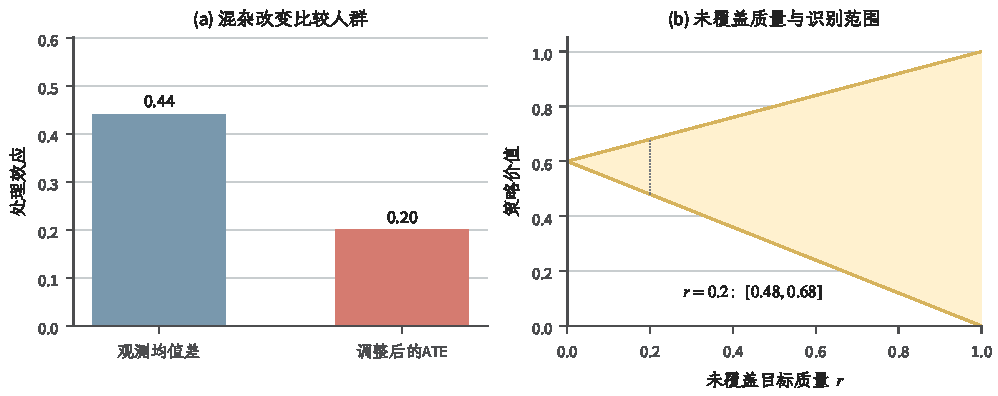
\includegraphics[width=\linewidth]{figures/math-preparation/probability-discrete/causal-confounding-coverage.pdf}
  \caption{两个独立的因果教学构造。左图复用混杂算例，比较观测均值差\(0.44\)与调整后的ATE \(0.20\)。右图假定结果范围为\([0,1]\)、已覆盖部分平均收益为\(0.6\)，绘制式~\eqref{eq:causal-policy-value-bounds}的范围\([0.6(1-r),0.6(1-r)+r]\)。阴影是总体识别范围，不是抽样置信带；两面板也不表示同一数据集。}
  \label{fig:causal-confounding-coverage}
\end{figure*}

\subsection{线性混杂与潜在结果偏差函数}

未观测混杂留下的歧义可以用敏感性参数表达，而不必在“完全无混杂”和“完全不可知”
之间二选一。一个最小线性例子先显示偏差从哪里进入。设变量已经中心化，并令
\[
  T=\alpha U+\varepsilon_T,\qquad
  Y=\beta T+\gamma U+\varepsilon_Y,
\]
其中\(U,\varepsilon_T,\varepsilon_Y\)两两独立、方差有限，且
\(\operatorname{Var}(T)>0\)。把\(Y\)仅对\(T\)作总体线性回归，观测斜率为
\begin{equation}
  \beta_{\mathrm{obs}}
  =
  \frac{\operatorname{Cov}(T,Y)}{\operatorname{Var}(T)}
  =
  \beta+
  \gamma\frac{\alpha\operatorname{Var}(U)}{\operatorname{Var}(T)}.
  \label{eq:causal-linear-confounding-bias}
\end{equation}
\(\beta\)是该结构模型中的处理系数，后一项是共同原因同时进入处理和结果造成的混杂
偏差。若领域信息只支持该偏差的绝对值不超过\(\Lambda\)，则
\(\beta\in[\beta_{\mathrm{obs}}-\Lambda,\beta_{\mathrm{obs}}+\Lambda]\)。数据可估计
\(\beta_{\mathrm{obs}}\)，却不能在没有额外信息时把\(\alpha,\gamma\)各自分开；改变
函数形式也会改变这个敏感性参数的含义。

对非线性和异质效应，不存在一个普遍通用的斜率修正量。仍记
\[
  \mu_t(x)=\mathbb{E}[Y\mid T=t,X=x],\qquad
  e(x)=\mathbb{P}(T=1\mid X=x).
\]
对目标总体中满足\(0<e(x)<1\)且下列条件期望有限的\(x\)，定义两个选择偏差函数
\begin{align*}
  b_1(x)
  &=
  \mathbb{E}[Y(1)\mid T=1,X=x]
  -
  \mathbb{E}[Y(1)\mid T=0,X=x],\\
  b_0(x)
  &=
  \mathbb{E}[Y(0)\mid T=1,X=x]
  -
  \mathbb{E}[Y(0)\mid T=0,X=x].
\end{align*}
完整条件交换性~\eqref{eq:causal-conditional-exchangeability}蕴含
\(b_1(x)=b_0(x)=0\)。对本节的平均效应目标，后一个条件表达的是较弱的条件均值
交换性；它不能反推出两个处理组中的潜在结果完整条件分布相同。若要对目标总体平均，
上述重叠和有限期望条件还须对目标总体中的\(x\)几乎处处成立。一致性给出
\(\mathbb{E}[Y(1)\mid T=1,X=x]=\mu_1(x)\)，因而
\[
\begin{aligned}
  \mathbb{E}[Y(1)\mid X=x]
  &=
  e(x)\mu_1(x)
  +(1-e(x))\bigl(\mu_1(x)-b_1(x)\bigr)\\
  &=
  \mu_1(x)-(1-e(x))b_1(x).
\end{aligned}
\]
同理，
\[
  \mathbb{E}[Y(0)\mid X=x]
  =
  \mu_0(x)+e(x)b_0(x).
\]
所以条件效应满足
\begin{equation}
  \tau(x)
  =
  \mu_1(x)-\mu_0(x)
  -(1-e(x))b_1(x)-e(x)b_0(x).
  \label{eq:causal-selection-bias-function}
\end{equation}

若领域知识只支持
\[
  |b_1(x)|\leq\Gamma_1(x),\qquad
  |b_0(x)|\leq\Gamma_0(x),
\]
则由三角不等式，
\begin{align}
  \mu_1(x)-\mu_0(x)-\Delta(x)
  \leq\tau(x)
  \leq
  \mu_1(x)-\mu_0(x)+\Delta(x),
  \label{eq:causal-sensitivity-bounds}
\end{align}
其中
\[
  \Delta(x)
  =
  (1-e(x))\Gamma_1(x)+e(x)\Gamma_0(x).
\]
对\(X\)取平均便得到ATE的敏感性区间。这里的\(\Gamma_t\)不是由观测数据自动估计出的
误差条，而是对未观测选择差异强度的假设。敏感性分析应展示结论在多大
\(\Gamma_t\)下改变符号或越过决策阈值，而不是只报告一个方便的参数值。

\subsection{额外假设与识别集合收缩}

若有理由相信处理对每个单位都不会降低结果，即
\[
  Y(1)\geq Y(0),
\]
则ATE至少为零，可以把任何已有下界提高到零。这项\term{单调性}（monotonicity）
排除了受处理伤害的机制；它比“平均上看有益”更强。若只知道处理效应位于
\([-\rho,\rho]\)，则支持缺口中的\([-1,1]\)可替换为更窄范围。

跨环境信息也可能收紧识别集合。例如一个环境提供随机试验，另一个环境只提供目标总体
协变量分布；若条件处理效应在两环境间保持不变，并且协变量支持得到覆盖，就能把试验
效应重新加权到目标环境。机制不变、总体可比和支持覆盖分别是新增假设。仅观察到某个
预测关系在多个环境都稳定，不足以排除共同隐藏原因、选择机制或多个机制恰好同时变化。

识别集合及其区间包络还必须与\term{置信区间}区分。前者在总体分布已知时仍可能不是
单点，表达机制歧义；后者由有限样本产生，表达对总体量、识别集合或其端点的估计误差。
实际报告可以给出端点的置信范围，但不能把包络宽度与抽样误差合并后统一称为“模型
不确定性”，否则读者无法判断增加样本、改变设计或增加假设中的哪一种能够收紧结论。

\section{反事实与行动补救}
\label{sec:causal-counterfactual-recourse}

部分识别讨论总体效应还可能有哪些值。下面改变目标为一个已观测个体的另一种结果，
需要在实际世界和替代行动之间保持同一个外生背景。总体干预边缘不能确定这种配对，
因此即使总体效应已识别，个体反事实仍可能需要更强机制假设。

\subsection{反事实推断与个体背景}

总体干预分布重新从外生背景总体中抽取个体，回答“若所有人采用处理\(t\)，平均会怎样”。
\begin{definition}[SCM中的反事实变量]
  \label{def:causal-counterfactual}
  设无环SCM的自然解映射为\(F\)，行动\(a\)替换指定结构方程后得到解映射\(F^a\)。在同一个外生背景\(\bm U\)上，\term{反事实}（counterfactual）变量定义为\(\bm V_a=F^a(\bm U)\)。给定实际证据\(\bm E\)后的反事实分布，是\(\bm V_a\)关于该证据的条件分布，而不是重新从背景总体抽取\(\bm U\)。
\end{definition}
它以已经观察到的个体为条件，回答“这个人在另一种处理下会怎样”。在SCM中，标准计算包含三个步骤：
\begin{enumerate}
  \item 根据实际观测更新外生背景\(\bm{U}\)的条件分布；
  \item 用目标行动替换相应结构方程；
  \item 在同一个背景分布下运行修改后的方程并计算结果。
\end{enumerate}
这三个步骤常称为背景推断、行动和预测。关键是实际世界与反事实世界共享同一外生背景；
若重新抽取一个人，计算的便是干预总体而不是个体反事实。

这三步可以统一写成分布推前。设无环SCM在自然机制下的解映射为
\(\bm{V}=F(\bm{U})\)，事实证据为\(\bm{E}=\bm{e}\)，行动\(a\)替换若干结构方程后得到
解映射\(F^a\)。若所在空间允许选取正则条件分布
\(P_{\bm{U}\mid\bm{E}=\bm{e}}\)，则对任意可测集合\(B\)，
\begin{equation}
  \begin{aligned}
  \mathbb{P}(\bm{V}_a\in B\mid\bm{E}=\bm{e})
  &=
  \left(F^a_{\#}
    P_{\bm{U}\mid\bm{E}=\bm{e}}\right)(B)\\
  &=
  \int
  \mathbb{I}\{F^a(\bm{u})\in B\}\,
  P_{\bm{U}\mid\bm{E}=\bm{e}}(\mathrm d\bm{u}).
  \end{aligned}
  \label{eq:causal-counterfactual-pushforward}
\end{equation}
其中\(F^a_{\#}P\)表示把分布\(P\)经映射\(F^a\)推前。第一步由事实证据更新背景分布，
第二步只改变映射，第三步把同一个背景后验推到反事实结果空间。连续证据点通常概率为零，
此时等式按正则条件分布的版本理解，并只保证对证据分布几乎处处的\(\bm{e}\)成立。零概率证据点的具体条件值还需要指定版本或额外结构，不能由条件概率的积分恒等式唯一决定。

考虑教学模型
\begin{equation}
  X=U_X,\qquad
  T=f_T(X,U_T),\qquad
  Y=2X+3T+U_Y.
  \label{eq:causal-counterfactual-linear-example}
\end{equation}
某人实际观测为\(X=2,T=0,Y=5\)。由结果方程反推出
\(U_Y=5-2\times2-3\times0=1\)。若保持该人的\(X,U_Y\)不变，把处理设为\(1\)，
则
\[
  Y_{T\leftarrow1}=2\times2+3\times1+1=8.
\]
差值\(3\)来自该结构方程中处理的直接作用。若结果方程或\(U_Y\)不能由观测唯一确定，
反事实结果应是条件分布或取值范围，而不是强行给出\(8\)这样的点值。

\begin{example}[两点背景后验的反事实推前]
  \label{ex:causal-two-point-background-posterior}
  令背景变量\(U\in\{u_{\mathrm L},u_{\mathrm H}\}\)的先验概率各为\(1/2\)。事实世界
  观察到二元信号\(S=1\)，且
  \[
    \mathbb{P}(S=1\mid U=u_{\mathrm H})=\frac34,\qquad
    \mathbb{P}(S=1\mid U=u_{\mathrm L})=\frac14.
  \]
  Bayes公式给出
  \[
    \mathbb{P}(U=u_{\mathrm H}\mid S=1)=\frac34,\qquad
    \mathbb{P}(U=u_{\mathrm L}\mid S=1)=\frac14.
  \]
  设行动\(a\)下的结果映射满足
  \(F_Y^a(u_{\mathrm L})=2\)与\(F_Y^a(u_{\mathrm H})=6\)。
  式~\eqref{eq:causal-counterfactual-pushforward}于是给出
  \[
    \mathcal L(Y_a\mid S=1)
    =\frac14\delta_2+\frac34\delta_6,
    \qquad
    \mathbb{E}[Y_a\mid S=1]=5.
  \]
  若忽略事实信号并从背景先验重新抽取个体，干预总体分布则是
  \(\frac12\delta_2+\frac12\delta_6\)，均值为\(4\)。两个答案使用同一行动映射，
  差别只在于反事实保留了由事实证据得到的背景后验。
\end{example}

\subsection{干预边缘与跨世界配对}

即使随机试验分别识别了\(Y(0)\)和\(Y(1)\)的边缘分布，也未必识别它们怎样在同一个体
上配对。设两种干预下的结果都服从\(\operatorname{Bernoulli}(1/2)\)。模型甲让一半
单位满足\((Y(0),Y(1))=(0,0)\)，另一半满足\((1,1)\)；模型乙让两类单位分别满足
\((0,1)\)和\((1,0)\)。两者在每种处理下都产生相同的结果分布，ATE也都为零，但模型甲
的个体效应恒为零，模型乙的个体效应则分别为\(1\)和\(-1\)。

图~\ref{fig:causal-cross-world-couplings}把这项歧义写成两张联合概率表。每张表的行和、列和都相同，但正质量落在不同格子上。用定义~\ref{def:information-coupling}的语言，两者是同一对干预边缘的不同耦合。对已知\(Y(0)=0\)的单位，模型甲给\(Y(1)=0\)，模型乙给\(Y(1)=1\)；边缘相同并未确定这项条件反事实。
\begin{figure}[htbp]
  \centering
  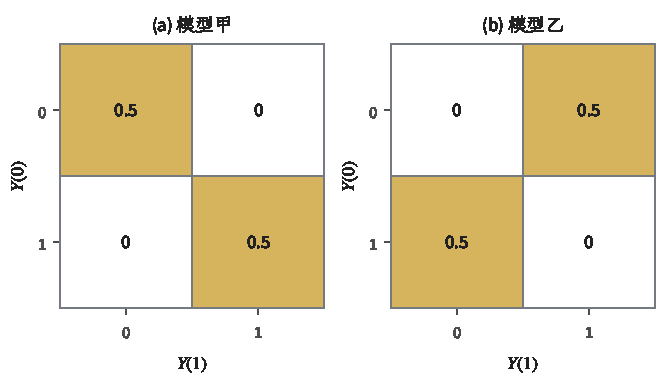
\includegraphics[width=\linewidth]{figures/math-preparation/concept-revision-probability/causal-cross-world-couplings.pdf}
  \caption{相同干预边缘的两种跨世界配对（教学构造的联合概率图）。行对应\(Y(0)\)，列对应\(Y(1)\)，格内数字为联合概率；两图的每个行和、列和均为\(1/2\)。模型甲个体效应恒为零，模型乙个体效应等概率取\(1,-1\)，而两者ATE均为零。这些联合表是相容机制的构造，并非从随机试验中直接观测到的数据。}
  \label{fig:causal-cross-world-couplings}
\end{figure}

两套配对机制连完整随机试验的两组边缘分布也无法区分。若要回答“事实结果为零的这个
单位在另一处理下会怎样”，还需要跨世界联合结构、重复干预、机制限制或相应的部分识别。
这一区别说明，干预分布的点识别不会自动传递给条件个体反事实。

\subsection{输入修改与现实行动}

对一个预测器\(\widehat y=f(\bm{x})\)，把输入字段\(t\)从\(0\)改成\(1\)并重新计算，
只得到
\[
  f(x,t=1)-f(x,t=0).
\]
它描述已训练函数对输入替换的响应。现实行动还可能改变处理的后继变量，并受到资源、
时间和可行域约束。若培训会提高技能，又减少当期工作时间，只修改“是否培训”一列而把
技能和时间固定，通常不是任何可实现世界。

\begin{definition}[因果行动补救]
  \label{def:causal-recourse}
给定事实证据、可实施行动集合\(\mathcal A(x)\)、结构机制、成本\(c(a;x)\)与目标决策集合\(G\)，\term{行动补救}（algorithmic recourse）寻找能使干预后的决策落入\(G\)的可行行动；因果行动补救用同一背景下的干预状态\(\bm V_a\)评价这项成功条件。
\end{definition}
因果补救
需要在结构模型中施加行动，让所有后继变量按机制共同变化，再把新状态送入决策系统。
若事实证据唯一确定了外生背景\(\bm u\)，其优化形式可以写成
\begin{equation}
  \min_{a\in\mathcal{A}(x)}
  c(a;x)
  \quad\text{使得}\quad
  d\bigl(\bm{V}_{a}(\bm{u})\bigr)
  \text{达到目标结果},
  \label{eq:causal-recourse-objective}
\end{equation}
其中\(\mathcal{A}(x)\)是该个体可实施的行动集合，\(c\)是行动成本，
\(\bm{V}_a(\bm{u})\)是同一背景下干预后的状态，\(d\)是最终决策规则。
低输入距离不等于低行动成本，不可改变属性也不应被当作建议。

事实证据通常只给出背景后验
\(P_{\bm U\mid\bm E=\bm e}\)，此时对某个候选\(\bm u\)成功并不保证行动对该个体
可靠。给定可容许失败概率\(\alpha\in[0,1]\)，一种概率型目标是要求
\[
  \mathbb{P}\!\left(
    d(\bm V_a(\bm U))\text{达到目标结果}
    \mid \bm E=\bm e
  \right)
  \geq 1-\alpha.
\]
若要求稳健保证，则可进一步要求后验支持中的每个背景都达到目标。概率约束与最坏情形
约束利用的是同一个背景后验，但后者更保守；二者都比只选一个候选背景检验行动更强。

补救还具有时间和策略边界。多人同时采取建议可能改变价格、名额或审核规则；决策系统
更新后，旧补救未必仍有效；执行成本与成功概率也可能因群体而异。因此，找到一个能翻转
当前模型输出的邻近输入，只证明了当前预测边界的局部性质，不自动证明建议可行、持久或
公平。

\subsection{反事实公平与不可识别性}

反事实公平比较同一个外生背景下，改变受保护属性后预测分布是否保持。设受保护属性为
\(A\)，实际观测为\((X=x,A=a)\)。\begin{definition}[反事实公平]
  \label{def:causal-counterfactual-fairness}
在已指定的SCM与预测规则下，反事实公平要求：对每个允许的替代属性\(a'\)和每个可测预测值集合\(B\)，下列等式对事实证据分布几乎处处的\((x,a)\)成立：
\begin{equation}
  \mathbb{P}\bigl(
    \widehat Y_{A\leftarrow a}\in B
    \mid X=x,A=a
  \bigr)
  =
  \mathbb{P}\bigl(
    \widehat Y_{A\leftarrow a'}\in B
    \mid X=x,A=a
  \bigr).
  \label{eq:causal-counterfactual-fairness}
\end{equation}
\end{definition}
实际观测用于推断背景，随后两个世界共享该背景。只在数据表中替换\(A\)，同时固定所有
由\(A\)产生的后继变量，检验的是不同对象。

个体反事实通常比平均干预效应需要更强结构。第
~\ref{sec:causal-observation-generation}节的两套模型观测分布相同，却对
\(T\leftarrow1\)给出不同后果；即使某些平均效应通过额外设计得到识别，同一个体的
\((Y(0),Y(1))\)联合关系仍可能没有被确定。若多个SCM都与观测和试验结果相容，应在这些
模型上报告反事实或补救结论的范围。一个生成模型能够产出清晰的“另一世界”样本，只说明
它选定了一套机制，不说明该机制已由数据唯一识别。

\section{结构发现与假设检验}
\label{sec:causal-structure-discovery}

前面的效应分析先给定生成结构，再问目标能否识别。本节反过来询问数据能排除哪些结构。
这是推断生成假设的一条独立支线：条件独立只能在Markov性、忠实性与观测制度等条件下
限制候选图，通常不能仅凭观测确定所有箭头方向。它所留下的结构歧义会再进入效应识别。

\subsection{Markov性、忠实性与三点结构}

定义~\ref{def:causal-d-separation}和因果Markov性允许从图推出条件独立。结构发现要
反向利用观测独立性排除候选图，因此还要限制那些由参数巧合产生、却不对应路径阻断的
独立关系。

\begin{definition}[相对于DAG的忠实性]
  \label{def:causal-faithfulness}
  分布\(P\)相对于DAG \(\mathcal G\)满足\term{忠实性}（faithfulness），若对任意两两不交的节点集\(A,B,S\)都有
  \[ \bm V_A\perp\bm V_B\mid\bm V_S
       \quad\Longrightarrow\quad A\perp_{\mathcal G}B\mid S. \]
\end{definition}
它要求分布中出现的条件独立都由图结构解释，而不是由特殊参数抵消、确定性约束或误差相关偶然产生。因果Markov性说明图蕴含
哪些独立性，忠实性允许从观察到的独立性反推图上缺少哪些连接。前者不自动推出后者。

回看图~\ref{fig:causal-local-path-patterns}，面板(a)的共同原因和面板(b)的中介链在
给定中间节点后都会关闭；把中介链的两条箭头同时反向，这一条件独立模式也不变。因此，
忽略节点名称后的三种结构
\(X\to Z\to Y\)、\(X\leftarrow Z\leftarrow Y\)和\(X\leftarrow Z\to Y\)都蕴含
\[
  X\perp Y\mid Z,
\]
并且一般不蕴含\(X\perp Y\)。仅靠这些条件独立关系，无法判断中间变量是传递作用还是
共同原因。相反，面板(c)的碰撞结构通常蕴含\(X\perp Y\)，而给定中间节点后可能相关，
所以可以由不同的独立模式与前三者区分。

\subsection{观测结构与Markov等价类}

\begin{definition}[Markov等价与等价类]
  \label{def:causal-markov-equivalence}
若同一节点集上的两张有向无环图具有完全相同的d-分离关系，就称它们
\term{Markov等价}（Markov equivalent）；与给定图Markov等价的全部有向无环图组成
它的\term{Markov等价类}（Markov equivalence class, MEC）。
\end{definition}
两张图Markov等价，
当且仅当它们具有相同的\term{骨架}（skeleton），即忽略方向后有相同的邻接边，并且
具有相同的\term{无屏蔽碰撞结构}（unshielded collider）：形如
\(X\to Z\leftarrow Y\)，且\(X\)与\(Y\)不相邻\scite{pgm-structure-learning-chickering2002}因而，在因果Markov性与忠实性等
假设下，纯观测条件独立信息通常只能识别一个Markov等价类，而不是唯一有向图。

局部差异已经由图~\ref{fig:causal-local-path-patterns}展示：链和共同原因具有相同骨架，
且都没有无屏蔽碰撞点；碰撞结构则改变了条件化前后的连通模式。对较大图，还要像图
~\ref{fig:causal-d-separation-paths}那样检查全部路径，而不能只比较一个三点片段。
相同骨架且没有新增无屏蔽碰撞点的方向变化，才可能留在同一个等价类中。

必要性要比较全部路径，而不能把一个三点片段当成完整图。在DAG中，非相邻的两点总存在
一个不含端点的d-分离集：选取其中一个节点，使另一点是它的非后代，再以所选节点的父
节点集作分离集。进入所选节点的路径被父节点阻断；从它向外出发而到达非后代的路径必有
一个后代碰撞点，该碰撞点及其后代不可能属于所选节点的父节点集，因而也被阻断。直接
相邻两点之间的单边路径却不能被任何不含端点的集合阻断，所以骨架不同必导致分离关系
不同。

对于无屏蔽三点结构\(X-Z-Y\)，两端不相邻，故存在分离集。若中点不是碰撞点，每个
分离集都必须包含\(Z\)，否则这条长度为二的路径仍开放；若中点是碰撞点，任何分离集
都不能包含\(Z\)，否则该路径被打开。因此，同一骨架上不同的无屏蔽碰撞结构也必定
给出不同分离关系；这个判断允许图中存在其他路径。

充分性需要控制较长路径，这里引用完整的结构判据，不把局部因子重写当作充分性证明
\scite{pgm-structure-learning-chickering2002}下面的覆盖边反转解释已确定的等价类内部
怎样改变方向。一条边\(X\to Y\)若满足
\(\operatorname{pa}(Y)=\operatorname{pa}(X)\cup\{X\}\)，称为
\term{覆盖边}（covered edge）。覆盖边反转定理说明，反转这种边后仍是DAG，且保留
全部d-分离关系\scite{pgm-structure-learning-chickering2002}这一单步变换也可以从相应的两个局部因子理解：
\[
  p(x\mid\operatorname{pa}(X))
  p(y\mid x,\operatorname{pa}(X))
  =
  p(y\mid\operatorname{pa}(X))
  p(x\mid y,\operatorname{pa}(X))
\]
重新表示，不改变它们合起来的条件联合分布。上述等式解释单步的分布重参数化，却还
没有证明两个指定图之间存在整条变换序列。完整的等价类变换定理进一步保证：任意两张
Markov等价DAG均可通过有限次覆盖边反转相互到达，每个中间图都保持无环和等价。
这一变换结论以两图已经Markov等价为前提，说明类内变换的可达性，不能代替上述
结构判据的充分性证明\scite{pgm-structure-learning-chickering2002}

等价类可以用部分有向图表示：在所有等价图中方向一致的边保留箭头，方向仍可变化的边
保持无向。算法输出这种等价类不是“尚未优化好”，而是忠实、无环且无潜在混杂等假设下
观测分布本身留下的总体歧义。增加同一观测分布的样本，只会更准确地判断独立关系，不会
为等价类内部凭空增加方向信息。

\subsection{潜在混杂、选择与有限样本检验}

若所有变量的共同原因都已观测，就称满足因果充分性。潜在共同原因会使两个可观测节点
相关，却无法由其中一方向另一方的箭头正确表示。允许潜在混杂时，结构发现的输出通常要
扩展为带不同端点标记的部分图，用来区分确定的祖先关系、可能方向和无法排除的隐藏共同
原因。测量误差和按碰撞点选择样本也会改变条件独立模式，不能简单解释为新因果边。

总体条件独立在有限样本中还要通过检验或评分近似判断。以
\(H_0:V_i\perp V_j\mid\bm V_S\)为原假设，并假定约束型算法在未拒绝条件独立时
删除候选边：第一类错误把真实独立误判为依赖，可能保留虚假边；第二类错误把实际依赖
误判为独立，可能删除真实边。后续搜索和定向规则还可能传播这些错误，而评分型算法未必
能直接套用这一对应。高维条件集合又使每个分层中的有效样本减少，接近零但非零的依赖
尤其难与独立区分。结构学习的一致性结论需要同时说明真实分布的Markov与忠实条件、
检验或评分随样本增长的性质、候选图范围及搜索是否足以找到目标。算法返回一张确定图，
不代表方向的不确定性已经消失。

\subsection{干预、跨环境信息与方向识别}

干预会切断目标变量原有的进入机制。若在观察数据中\(X\)与\(Y\)相关，而随机设置
\(X\)后\(Y\)的分布随设置值改变，这为\(X\)位于\(Y\)上游提供了观测关联之外的证据。
对不同节点实施干预可以缩小Markov等价类；若干预目标未知、执行不完全或干预同时改变
其他机制，则必须把这些不确定性纳入模型。

跨环境信息也能提供约束。若不同环境只改变少数外生分布，而某个条件机制保持不变，
机制不变性可以帮助比较候选方向。但“关系稳定”单独不是充分条件。隐藏共同原因可能在
所有已观察环境中都稳定，环境变化也可能太弱而没有打破错误方向；选择规则若同步变化，
还可能制造新的稳定关联。应明确哪些机制允许变化、环境标签是否影响结果，以及稳定性
是作为假设、检验对象还是经验线索使用。

结构发现因而需要多类证据协作。条件独立限制观测等价类，受控干预主动打破部分歧义，
机制知识排除不合理方向，敏感性分析检查结论对潜在混杂、弱依赖和选择机制的变化。
这些证据可以互相补充，却不能由一项代理另一项。对于反馈环、随时间变化的机制或处理
定义不稳定的系统，无环静态SCM本身也可能不适用，需要改用动态或循环因果模型并重新
定义干预。

\section{本章小结}
\label{sec:causal-inference-summary}

观测分布描述自然机制运行时变量怎样共同出现，干预分布描述替换某个生成机制后的总体
结果，个体反事实则在实际观测推断出的同一背景下比较另一行动。两套结构机制可以拥有
完全相同的观测分布，却给出不同干预和反事实；这说明预测精度、样本规模和优化能力都
不能代替生成假设。

潜在结果把不同处理下的结果并列表示，一致性连接实际处理与观察结果，无干扰和处理版本
唯一性保证目标定义清楚。随机分配直接建立交换性；观察研究则通常需要条件交换性与支持
重叠。正值性只需覆盖目标总体中目标行动会使用的协变量--行动组合，不要求目标之外处处
重叠。结合这些条件，调整公式和逆概率表示把ATE化成可观测分布的泛函。识别只说明总体
目标能否唯一确定，有限样本估计和数值计算还需各自的误差条件。

当交换性、重叠或机制知识不足时，部分识别保留所有相容答案。有界结果给出不依赖无混杂
的锐界，支持缺口按缺口人群或目标策略未覆盖的概率质量扩大范围，偏差函数把未观测混杂
的强度转成敏感性区间。单调性、效应范围或跨环境机制不变可以收紧集合，但每项收紧都
来自新增假设。一般识别集合未必是区间，上下界只给出它的区间包络；识别集合表达总体
机制歧义，置信区间表达有限样本误差，二者不能混为同一种不确定性。

结构发现同样受识别边界约束。因果Markov性把图结构连接到条件独立，忠实性才允许从独立
关系反推结构；纯观测数据通常只能确定Markov等价类，潜在混杂、选择和测量误差还会扩大
歧义。干预、跨环境变化和机制知识能够补充方向证据，但必须写清各自保持和改变了什么。
因此，因果推断的核心不是为关联加上箭头，而是对每个干预、效应或反事实结论列明目标、
生成假设、可用证据和仍未被决定的范围。此前第~\ref{chap:combinatorics}章已区分
有限候选的计数、可行性、最优性与计算复杂度；接下来的第~\ref{chap:graph-theory}章
会以顶点与边为对象，系统处理路径、分离与图分解。这些图结构可以支持因果图上的计算，
其因果解释仍须由本章的生成与干预假设确定。
第~\ref{chap:decision-theory-and-dynamic-risk}章把单步干预扩展为序贯行动和价值递推；
\BookChapterRef{chap:trust-fairness}{第二卷“基础、理论和可信性”的“公平性”章}与
\BookChapterRef{chap:trust-interpretability}{第二卷“基础、理论和可信性”的“可解释性”章}
则分别回用反事实目标和行动补救，并重新加入规范要求与实际验证条件。


\bookpart{图论}{Graph Theory}
\label{part:discrete-mathematics-and-graph-theory}

\chapter{图论}
\label{chap:graph-theory}
有限变量的约束和目标往往只涉及少数变量，却需要在全部赋值上求和或择优。图能记录这些局部关系，但读者还需要判断：哪些关系可以分开计算，哪些结构支持精确求解，以及哪些信息在分割、扩散或重编号后仍然保留。
这些是本章考察图的三个主要用途。

第~\ref{chap:combinatorics}章用\(z_1,\ldots,z_4\)四个二值变量说明有限变量、约束
与目标。本章不增加变量，而是直接从式~\eqref{eq:comb-running-cnf}的约束作用域构造
\term{原始关系图}（primal graph）：每个二值变量对应一个顶点，同一子句中的任意两个
变量相连。前两个子句给出边\(\{1,2\}\)，第三个子句给出边\(\{1,3\}\)，三变量
子句\(\neg z_4\lor z_2\lor z_3\)则使\(2,3,4\)三个顶点两两相连；这样的顶点集合
后文称为团。图只记录哪些变量需要在同一个局部约束中共同处理；三变量子句仍是一个三元
约束，不能把这三条边误解为三个与原子句等价的二元约束。

贯穿例固定第~\ref{chap:combinatorics}章的四个二值变量：
\[
  z_i\in\{0,1\},\qquad i\in V=\{1,2,3,4\}.
\]
讨论不依赖二值性的图算法时，用有限集合\(\mathcal{Z}_i\)表示变量\(z_i\)的一般
取值域；贯穿例对应\(\mathcal{Z}_i=\{0,1\}\)。
图~\ref{fig:graph-theory-running-graph}中的边表示哪些变量共同出现在某个约束中。
边集合为
\begin{equation}
  E=\bigl\{\{1,2\},\{1,3\},\{2,3\},\{2,4\},\{3,4\}\bigr\}.
  \label{eq:graph-theory-running-edges}
\end{equation}
这张图很小，却包含本章需要分开的几种作用。两个三角形\(\{1,2,3\}\)与
\(\{2,3,4\}\)共享接口\(\{2,3\}\)，所以固定接口后，只含\(z_1\)与只含\(z_4\)
的局部计算可以分开。若过早消去顶点\(2\)，原本不相邻的顶点\(1,4\)会在中间结果中
直接联系。同一连接结构可以承载硬约束、概率、得分、距离或容量，但这些数值语义并不
由图本身决定。

\begin{figure}[htbp]
  \centering
  \begin{tikzpicture}[text=FigureInk,
    vertex/.style={circle,draw=FigureStroke,fill=FigureYellowFill,line width=1pt,
      minimum size=8mm,inner sep=0pt,font=\figurefont\footnotesize},
    edge/.style={draw=FigureStroke,line width=1.1pt}
  ]
    \node[vertex] (x2) at (0,1.15) {\(z_2\)};
    \node[vertex] (x3) at (0,-1.15) {\(z_3\)};
    \node[vertex] (x1) at (-2.1,0) {\(z_1\)};
    \node[vertex] (x4) at (2.1,0) {\(z_4\)};
    \draw[edge] (x1)--(x2);
    \draw[edge] (x1)--(x3);
    \draw[edge] (x2)--(x3);
    \draw[edge] (x2)--(x4);
    \draw[edge] (x3)--(x4);
  \end{tikzpicture}
  \caption{由第~\ref{chap:combinatorics}章约束作用域导出的变量关系图。每条边表示
  两个变量共同出现在至少一个约束中；共享边\(\{2,3\}\)是左右两个三角形的接口。
  边权、方向与关系的数值含义需要另行给出。}
  \label{fig:graph-theory-running-graph}
\end{figure}

本章先建立表达关系和判断可达性的共同基础，再明确局部函数需要回答的查询。
在查询语义已知后，消元、弦图与树分解才用于分析中间表的规模。
条件独立查询另有一套路径规则，因而单独比较有向与无向分离；它依赖图结构，却不能由计算分解自动推出。
随后讨论路径、连接、流量、匹配和二值能量这些不同优化目标，分别说明精确算法成立的条件。
图上的数值信号以及与编号无关的结构比较则提供另外两种用途：前者研究平滑、划分与扩散，后者检验表示能否区分不同连接结构。

\section{关系的表示与可达性}
\label{sec:graph-theory-objects-representations}

不同任务会反复使用顶点、边、路径和矩阵表示。这里先建立这些共同语言：边记录直接关系，路径判断关系能否延伸，矩阵则将邻域汇总写成线性运算。遍历负责找到可达区域与合法处理次序，不预先赋予边概率或成本语义。

\subsection{顶点、边与图类型}

\term{无向图}（undirected graph）是二元组
\[
  \mathcal{G}=(V,E),
\]
其中\(V\)是顶点集合，\(E\)是由不同顶点组成的无序对集合。若
\(\{i,j\}\in E\)，就称\(i,j\)相邻，并把二者分别称为对方的邻居。顶点\(i\)的
\term{邻域}（neighborhood）与\term{度}（degree）分别为
\[
  N(i)=\{j\in V:\{i,j\}\in E\},\qquad d_i=|N(i)|.
\]
式~\eqref{eq:graph-theory-running-edges}定义的图中，
\(N(2)=\{1,3,4\}\)，而\(N(1)=\{2,3\}\)。这里采用不含自环、平行边的有限简单图；
若任务允许自环或同一对顶点间有多条边，必须把边集合改为相应的多重结构。

无向边表达对称关系。若关系具有先后或作用方向，就使用
\term{有向图}（directed graph）\(\mathcal{G}=(V,A)\)，其中
\(A\subseteq V\times V\)由有序对组成。\((i,j)\in A\)表示从\(i\)指向\(j\)，
不自动推出\((j,i)\in A\)。指向顶点\(j\)的弧称为\(j\)的入边，入边条数称为
\term{入度}（in-degree）；从\(j\)指出的弧称为出边，其条数称为
\term{出度}（out-degree）。因果生成次序、状态转移和计算依赖通常需要有向边；
距离邻接或对称相似性通常使用无向边。

边还可以带有\term{权重}（weight）。无向加权图要求
\(w_{i,j}=w_{j,i}\)，有向加权图则允许二者不同。权重可以表示长度、容量、相似度
或局部代价；这些量对“权重大”的解释不同，所以每个算法都须重新声明权重语义。本章
不统一排除零权边：结构边集\(E\)记录哪些关系存在，而对无向非负权图，
\[
  E_+=\bigl\{\{i,j\}\in E:w_{i,j}>0\bigr\}
\]
称为\term{正权支撑}（positive-weight support）。当权重作为线性算子的系数时，
零权结构边不产生贡献，相关的谱与扩散结论因而取决于支撑图\(\mathcal{G}_+=(V,E_+)\)。

成对边有时仍不足以表达局部关系。若一个约束同时作用于\(\{2,3,4\}\)，把它拆成三条
边可能改变允许的赋值。此时使用\term{超图}（hypergraph），其超边可以包含两个以上
顶点。也可使用\term{二部图}（bipartite graph）把顶点分成两组，只允许跨组边。
变量与局部因子形成的因子图就是二部图，它保留了高阶关系同时涉及哪些变量。

图~\ref{fig:graph-theory-factor-scope}把同一个三元作用域画成两种表示。因子图保留“这三个变量属于同一个函数”，
原始关系图只保留“这三对变量各需共同处理”。从后一张图无法恢复原来究竟有一个三元函数，还是三个二元函数。

\begin{figure}[htbp]
  \centering
  \begingroup
\input{figures/math-preparation/reader-revision-graph/diagram-style}
\begin{tikzpicture}[text=FigureInk]
  \node[reader label] at (0,1.35) {(a) 三元因子};
  \node[reader factor] (f) at (0,0) {\(\phi_{2,3,4}\)};
  \node[reader vertex] (a) at (-1.35,0) {\(z_2\)};
  \node[reader vertex] (b) at (0,-1.05) {\(z_3\)};
  \node[reader vertex] (c) at (1.35,0) {\(z_4\)};
  \draw[reader edge] (a)--(f)--(c);
  \draw[reader edge] (b)--(f);
  \node[reader label] at (4.8,1.35) {(b) 原始关系图};
  \node[reader vertex] (x) at (3.45,0) {\(z_2\)};
  \node[reader vertex] (y) at (4.8,-1.05) {\(z_3\)};
  \node[reader vertex] (z) at (6.15,0) {\(z_4\)};
  \draw[reader edge] (x)--(y)--(z)--(x);
\end{tikzpicture}
\endgroup

  \caption{三元因子与原始关系图的区别。左侧方框代表一个依赖\(z_2,z_3,z_4\)的函数，连线表示变量属于其作用域；右侧只保留共同出现关系。右侧三条边不构成把该函数拆成三个二元函数的等价变换。}
  \label{fig:graph-theory-factor-scope}
\end{figure}

给定图\(\mathcal G\)和\(U\subseteq V\)，保留\(U\)中顶点及原图中两端都在\(U\)内的全部边或弧，
所得图称为\(U\)上的\term{诱导子图}（induced subgraph），记作\(\mathcal G[U]\)。
它允许删顶点，却不允许任意删去保留顶点之间的原有边；这个区别会用于弦图和祖先图。

\subsection{路径、环与连通性}

图中的\term{游走}（walk）是顶点序列
\(v_0,v_1,\ldots,v_k\)，相邻两项之间有边；顶点与边可以重复。若
\(v_0,\ldots,v_k\)两两不同，就得到\term{路径}（path）。长度是经过的边数；
在带长度的图上，路径长度改为边长之和。
无向图中的\term{环}（cycle）是长度\(k\geq3\)的闭游走
\(v_0,v_1,\ldots,v_k\)，其中\(v_0=v_k\)，而\(v_0,\ldots,v_{k-1}\)两两不同。
因此环只在首尾重复同一顶点，不与路径要求全部顶点互异的定义混用。

若任意两个顶点间都有路径，无向图称为\term{连通}（connected）。一般无向图可以唯一
分成若干极大的连通子图，称为连通分量。图
~\ref{fig:graph-theory-running-graph}连通，因为每个顶点都能经顶点\(3\)到达其他顶点；
\(1,2,3,1\)与\(2,3,4,2\)分别构成一个环。删除边\(\{1,2\}\)后图仍连通，
但第一个环消失。

连通且无环的无向图称为\term{树}（tree）。树中任意两点之间恰有一条简单路径：
两条不同路径从分开到重新会合的部分会构成环。含\(n\)个顶点的树恰有\(n-1\)条边，
若干棵互不相连的树组成森林。下面把路径唯一性和边数结论合在一起证明，因为二者分别
解释树为何适合递推，以及递推中为何不会遗漏额外连接。

\begin{theorem}[树的等价刻画]
  \label{thm:graph-theory-tree-characterizations}
  对含\(n\geq1\)个顶点的有限无向简单图，以下三条等价：
  \begin{enumerate}
    \item 图连通且无环；
    \item 任意两点之间恰有一条简单路径；
    \item 图连通，并且恰有\(n-1\)条边。
  \end{enumerate}
\end{theorem}

\begin{proof}
若图连通且无环，任意两点间至少有一条简单路径；若有两条不同的简单路径，从二者首次
分开处走到再次会合处便得到一个环，产生矛盾，故路径唯一。反过来，路径唯一已经包含
连通性；若图有环，环上相邻顶点之间既有该边，又有沿环另一侧的路径，与唯一性矛盾。

再证明边数。单顶点树有\(0\)条边。含至少两个顶点的有限树必有叶顶点：取一条最长
简单路径，端点若还有路径外邻居，就能延长该路径；端点若连接路径中的非相邻顶点，
又会形成环。删除叶顶点及其唯一关联边后仍是树，归纳得到边数
\((n-1)-1+1=n-1\)。树中任意边又位于其两端的唯一简单路径上，删除该边必使两端
断开。

最后，设图连通且有\(n-1\)条边。从任一顶点开始，每次加入一条连接“已加入顶点”与
“尚未加入顶点”的边；连通性保证只要还有顶点未加入，这样的边就存在。加入一个新顶点
不会形成环，重复\(n-1\)次便得到一棵覆盖全部顶点的树。该树已经使用原图的全部
\(n-1\)条边，所以原图与这棵树相同，因而无环。
\end{proof}

有向图中的路径必须顺着弧方向前进。\term{有向环}（directed cycle）是除首尾外顶点
互异、每一步都沿弧方向的闭游走。在不含自环的有向图中，有向环长度至少为\(2\)：
若\(i\to j\)与\(j\to i\)同时存在，二者已经构成有向环；这与无向简单图的环至少
包含三个顶点不同。不含有向环的图称为
\term{有向无环图}（directed acyclic graph, DAG）。DAG中的边可以规定偏序依赖，
但图中没有边的两个顶点不一定可以互换执行，它们还可能通过更长路径间接依赖。
后文的拓扑排序会把这种偏序扩展为一个线性次序。

有向图还需区分两种连通性。若任意有序顶点对\(i,j\)之间都有从\(i\)到\(j\)的
有向路径，图称为\term{强连通}（strongly connected）；若忽略弧方向后所得无向图
连通，则称为\term{弱连通}（weakly connected）。强连通蕴含弱连通，反向不成立。
例如单向链\(1\to2\to3\)弱连通，却不存在从\(3\)返回\(1\)的有向路径。

\subsection{邻接矩阵与线性映射}

给顶点固定次序\(1,\ldots,n\)，无向图的\term{邻接矩阵}（adjacency matrix）
\(\bm{A}\in\mathbb{R}^{n\times n}\)定义为
\[
  a_{i,j}=\begin{cases}
    w_{i,j},&\{i,j\}\in E,\\
    0,&\text{其他情形}.
  \end{cases}
\]
无权图取\(w_{i,j}=1\)。无向图使\(\bm{A}\)对称；有向图则令
\(a_{i,j}\)记录弧\(i\to j\)的权重，一般不对称。简单无向图没有自环，所以主对角线
为零。若允许结构边的权重为\(0\)，数值矩阵中的零条目不能区分零权边与无边，此时必须
把\(\bm{A}\)与边集\(E\)或一个邻接掩码一同保存；只有在所有结构边权非零时，
\(\bm{A}\)才单独确定边集。图~\ref{fig:graph-theory-running-graph}的邻接矩阵是
\begin{equation}
  \bm{A}=\begin{bmatrix}
    0&1&1&0\\
    1&0&1&1\\
    1&1&0&1\\
    0&1&1&0
  \end{bmatrix}.
  \label{eq:graph-theory-running-adjacency}
\end{equation}

邻接矩阵不只是存储表。对顶点数值
\(\bm{f}=(f_1,\ldots,f_n)^{\top}\)，
\[
  (\bm{A}\bm{f})_i=\sum_{j\in N(i)}w_{i,j}f_j
\]
汇总顶点\(i\)的邻居值，因此是第~\ref{chap:linear-algebra}章意义下的线性映射。
矩阵幂还记录游走：对无权图，
\((\bm{A}^k)_{i,j}\)等于从\(i\)到\(j\)长度为\(k\)的游走数。证明只需对\(k\)
归纳；矩阵乘法在中间顶点\(\ell\)上求和，恰好把长度\(k\)的游走与最后一条边拼接。
游走允许重复顶点，所以该数一般不等于简单路径数。对带权图，同一归纳说明
\[
  (\bm{A}^k)_{i,j}
  =\sum_{i=v_0\to v_1\to\cdots\to v_k=j}
  \prod_{r=1}^{k}w_{v_{r-1},v_r},
\]
即条目是所有长度\(k\)游走的权重乘积之和，而不再是游走条数。这个解释依赖通常的
加法与乘法；换用布尔或最小加法运算时，矩阵幂会回答可达性或固定边数最短成本等不同
问题，不能继续称为计数。

矩阵表示依赖顶点次序。若置换矩阵\(\bm{P}\)改变编号，同一无向图在新编号下表示为
\begin{equation}
  \bm{A}'=\bm{P}\bm{A}\bm{P}^{\top}.
  \label{eq:graph-theory-adjacency-relabel}
\end{equation}
矩阵元素的位置改变，连通、环和路径等图性质不应改变。反过来，并非任意相似变换都只是
顶点重编号；图重编号只允许置换矩阵，而第~\ref{chap:matrix-analysis}章中的一般换基
会混合顶点坐标，通常不再得到同一张离散图。

还可以给每条无向边任取一个方向，构造\term{关联矩阵}（incidence matrix）
\(\bm{B}\in\mathbb{R}^{|V|\times|E|}\)：边\(e:i\to j\)对应列在\(i\)处取\(1\)、
在\(j\)处取\(-1\)，其余为零。反转临时方向只会把该列乘\(-1\)，不改变后文的
\(\bm{B}\bm{W}\bm{B}^{\top}\)。邻接矩阵为每对顶点预留位置，适合稠密线性运算；
邻接表只存每个顶点实际相邻的对象，空间为\(O(|V|+|E|)\)，更适合稀疏图遍历；
关联矩阵则显式保留“哪条边连接哪些顶点”，便于表达边差分。在结构边权均非零，或为
邻接矩阵另附边集或掩码时，三种表示保留同一个图对象，但直接支持的计算和存储成本不同。

\subsection{图遍历与拓扑次序}

\term{广度优先搜索}（breadth-first search, BFS）从起点\(s\)出发，先访问距离
\(s\)为一条边的顶点，再访问距离为两条边的顶点。维护一个先进先出队列，并在顶点首次
入队时标记它，可以保证每个顶点至多入队一次、每条边至多检查常数次。因此使用邻接表时，
时间复杂度为\(O(|V|+|E|)\)\scite{math-cormen2022algorithms}每个非起点顶点首次
被发现时记录一条父边，这些父边不成环，并在所有可达顶点上构成一棵搜索树；队列、已访问
集合和父边分别回答“接下来处理谁”“谁已处理过”和“如何恢复发现路径”。

对无权图，BFS首次发现顶点\(v\)时记录的层数就是从\(s\)到\(v\)的最短路径长度。
证明按队列层次归纳：处理第\(k\)层顶点时，所有更短路径的终点已经处理；新发现邻居有
一条长度\(k+1\)的路径。若它存在更短路径，其倒数第二个顶点应位于更早层，并会更早
发现它，产生矛盾。带一般边长时，边数最少不等于总长度最小，BFS便不再适用。

\term{深度优先搜索}（depth-first search, DFS）沿一条尚未探索的边持续深入，无法
继续时回退。它同样能在线性时间内找连通分量，还能依据进入与退出时间识别有向图中的
回边。若DFS遇到一条指向当前递归栈内顶点的弧，就得到一个有向环；若没有这种回边，
按退出时间逆序排列顶点便得到拓扑序。

拓扑序与有向无环性的等价关系是图论中的基本结构结论\scite{math-diestel2017graph}
\begin{theorem}[DAG的拓扑排序]
  \label{thm:graph-theory-topological-order}
  有限有向图存在拓扑序，当且仅当它不含有向环。拓扑序是顶点的一个排列，使每条弧
  \(i\to j\)中\(i\)都排在\(j\)之前。
\end{theorem}

\begin{proof}
若存在有向环
\(v_1\to v_2\to\cdots\to v_k\to v_1\)，拓扑序将依次要求
\(v_1\)在\(v_2\)前、\(v_2\)在\(v_3\)前，最终又要求\(v_k\)在\(v_1\)前，
不可能同时满足。

反过来，设图无有向环。图中必有入度为零的顶点；否则从任意顶点\(v\)出发，总能选择
当前顶点的一条入边\(u\to v\)，并反向追溯到其起点\(u\)。顶点数有限，追溯中必有
顶点重复，而重复段按原弧方向组成有向环，产生矛盾。删除一个入度为零的顶点及其出边，
剩余图仍无环。重复这一过程直到图为空，删除次序就是拓扑序。每次若用队列维护新出现的
零入度顶点，全部过程只检查每个顶点和每条弧常数次。
\end{proof}

拓扑序一般不唯一。两个互相不可达的顶点可以有多种相对次序；这反映偏序未规定它们的
先后，而不是算法给出了矛盾答案。

\section{从局部函数计算全局查询}
\label{sec:graph-theory-semiring-dynamic-programming}

图只记录哪些变量共同出现。要开始计算，还必须知道输出是总权重、某个变量的边缘量，还是最佳配置。先明确这个目标，再说明局部组合与汇总怎样代替全部赋值上的枚举。

\subsection{查询目标与需要保留的变量}

同一局部数值表可以回答不同问题：把它解释为权重，可以求总权重或最高权重；解释为成本，则可以求最低成本。
查询还须指定输出。若要知道某个变量的边缘分布，就保留这个变量，汇总其余变量；若只要全局最优值，才汇总全部变量。
因此，“消去变量”是把它对指定输出的贡献合并到剩余函数中，并非删掉一个约束或忽略它的影响。

一个两变量小表可以直接核对运算改变了什么。令
\[
  g(x,y)=
  \begin{array}{c|cc}
    &y=0&y=1\\ \hline
    x=0&1&3\\
    x=1&2&4
  \end{array}.
\]
把四个表项视为非负权重时，和积查询给出
\(\sum_{x,y}g(x,y)=10\)，最大积查询在这里只有一个局部因子，给出
\(\max_{x,y}g(x,y)=4\)及见证\((1,1)\)。把同一组数字改解释为成本，最小加法查询
给出\(\min_{x,y}g(x,y)=1\)及见证\((0,0)\)。这三个答案来自同一作用域，却对应
不同问题；数值表本身不能决定应选哪一种半环。


以这张表为例，求和消去\(x\)得到\(m(y)=\sum_xg(x,y)\)，即
\(m(0)=3\)、\(m(1)=7\)。新表只有两个条目，却仍保留了每个\(y\)对应的全部权重；
再对\(y\)求和才得到\(10\)。如果\(g/10\)是联合概率表，\(m(y)/10\)就是\(y\)的边缘概率。
若把求和换成取最大值，则得到\(m(0)=2\)、\(m(1)=4\)：它保留的是各个\(y\)的最佳权重，不能再解释为边缘概率。
这一区别决定后面的消元应采用哪一种汇总运算。

\subsection{组合局部项与汇总候选值}

对一个固定赋值，需要组合同时成立的局部项；跨不同赋值，则需要汇总候选结果。
普通权重分别用乘法和加法，成本分别用加法和最小值。
为了让同一局部算法适用于这些选择，把组合记为\(\otimes\)，汇总记为\(\oplus\)。
局部计算能够代替全局枚举的关键规则是分配律：与某个变量无关的项，可以移出对该变量的汇总。

\begin{definition}[交换半环]
\label{def:graph-theory-semiring}
\term{半环}（semiring）$(\mathcal S,\oplus,\otimes,e_{\oplus},e_{\otimes})$由集合、两种运算及各自的单位元组成。本章使用交换半环，对所有$a,b,c\in\mathcal S$要求：$\oplus$与$\otimes$各自结合且交换，并分别以$e_{\oplus}$与$e_{\otimes}$为单位元；$\otimes$对$\oplus$分配，即
\[
 a\otimes(b\oplus c)=(a\otimes b)\oplus(a\otimes c);
\]
且$a\otimes e_{\oplus}=e_{\oplus}$。空汇总取$e_{\oplus}$，空乘积取$e_{\otimes}$。
\end{definition}

定义~\ref{def:graph-theory-semiring}不要求每个元素有加法逆元或乘法逆元。动态规划通常只需要组合、汇总和分配，不需要
做减法或除法。

三种与本章直接相关的半环为：
\[
\begin{array}{c|c|c|c|c}
  \text{用途}&\mathcal{S}&\oplus&\otimes&(e_{\oplus},e_{\otimes})\\
  \hline
  \text{总权重}&\mathbb{R}_{\geq0}&+&\times&(0,1)\\
  \text{最大权重}&\mathbb{R}_{\geq0}&\max&\times&(0,1)\\
  \text{最小成本}&\mathbb{R}\cup\{+\infty\}&\min&+&(+\infty,0)
\end{array}
\]
最大积中\(0\)既是\(\max\)的单位元，也是乘法吸收元。最小加法中
\(+\infty+c=+\infty\)，所以\(+\infty\)表示不可行路径或赋值。若最大积取对数，
还可得到\((\max,+)\)半环，其汇总单位元为\(-\infty\)、组合单位元为\(0\)。

布尔半环\((\{\mathrm{false},\mathrm{true}\},\lor,\land)\)则计算是否存在可行赋值。
同一个图结构因此能够回答“总共有多少权重”“最佳配置是什么”“是否存在配置”等不同
查询。结构相同不表示答案相同；运算是问题定义的一部分。

\subsection{局部因子的作用域与全局目标}

在贯穿关系图上，可以为每个顶点放置一元函数
\(\phi_i(z_i)\)，并在只考虑一元与成对局部项时为每条边放置成对函数
\(\phi_{i,j}(z_i,z_j)\)，形成
\begin{equation}
  F(\bm{z})=
  \bigotimes_{i\in V}\phi_i(z_i)\otimes
  \bigotimes_{\{i,j\}\in E}\phi_{i,j}(z_i,z_j).
  \label{eq:graph-theory-factorized-objective}
\end{equation}
这里的\(\otimes\)采用刚刚选定的组合运算。局部函数也称为因子；因子的作用域是它实际依赖的变量集合。
若要继续表示式~\eqref{eq:comb-running-cnf}的原始硬约束，第四个子句必须保留为
三元因子\(\phi_{2,3,4}(z_2,z_3,z_4)\)；式
~\eqref{eq:graph-theory-factorized-objective}是同一关系骨架上的成对专门情形，
不是把三元子句拆成三条边后的等价公式。
图说明每个局部项的作用域，却不说明这些函数是否为概率、约束指示、相似度或成本。
同一张图既可以计算总权重，也可以寻找最低成本配置；反过来，相同数值表若采用不同
作用域，也会产生不同的分解与计算代价。

图不会自动编码条件独立、因果或时间关系；这些语义还需生成规则、分布因子或结构假设。

若当前输出是变量\(z_4\)的边缘权重，则查询为
\[
  Q(z_4)=\sum_{z_1,z_2,z_3}F(\bm z),
\]
其中\(F\)须采用非负权重的乘积。\(z_1,z_2,z_3\)是需要汇总的内部变量，\(z_4\)是需要保留的输出变量。
当\(0<Z=\sum_{z_4}Q(z_4)<\infty\)时，\(Q(z_4)/Z\)才构成归一化边缘分布。
如果改问最低成本，目标则是\(\min_{\bm z}\bigl[\sum_i c_i(z_i)+\sum_{\{i,j\}\in E}c_{i,j}(z_i,z_j)\bigr]\)，
此时组合和汇总都要相应改变。消元是否有用，应以能否更省地计算这个已指定的输出为判断依据。

\subsection{借助分配律复用局部结果}

考虑贯穿图上的表达式~\eqref{eq:graph-theory-factorized-objective}。若要汇总全部赋值，
直接写成
\[
  Z=\bigoplus_{z_1,\ldots,z_4}F(\bm{z}).
\]
变量\(z_1\)只通过接口\((z_2,z_3)\)与其余变量联系，因此可以先计算
\begin{equation}
  m_{1\to\{2,3\}}(z_2,z_3)=
  \bigoplus_{z_1\in\mathcal{Z}_1}
  \phi_1(z_1)\otimes
  \phi_{1,2}(z_1,z_2)\otimes\phi_{1,3}(z_1,z_3).
  \label{eq:graph-theory-interface-message}
\end{equation}
对每个接口赋值\((z_2,z_3)\)，这个局部结果只需计算一次。变量\(z_4\)一侧可得到
同形消息\(m_{4\to\{2,3\}}(z_2,z_3)\)，最终只需在接口上组合两条消息和其余局部项。

这一步合法，不是因为图画成树枝形，而是因为\(\otimes\)对\(\oplus\)满足分配律。
若把与\(z_1\)无关、但可以依赖接口值的项记为\(c(z_2,z_3)\)，则
\[
  \bigoplus_{z_1}\bigl(c(z_2,z_3)\otimes g(z_1,z_2,z_3)\bigr)
  =c(z_2,z_3)\otimes\left(\bigoplus_{z_1}g(z_1,z_2,z_3)\right).
\]
图说明哪些项与\(z_1\)无关，代数规则则允许把它们移出汇总。动态规划的核心就是保存
接口变量上的局部结果，使后续不同部分复用同一个子问题答案。

树上的消息可以把这一直觉写成精确不变量。先考虑一棵树，并在顶点与边上分别放置
\(\phi_i(z_i)\)和\(\phi_{i,j}(z_i,z_j)\)。删除边\(\{u,v\}\)后，记包含\(u\)
的连通分量为\(T_{u\mid v}\)。从\(u\)发给\(v\)的消息定义为
\begin{equation}
  m_{u\to v}(z_v)=
  \bigoplus_{\bm{z}_{T_{u\mid v}}}
  \left[
    \bigotimes_{i\in T_{u\mid v}}\phi_i(z_i)
    \otimes
    \bigotimes_{\substack{\{i,j\}\in E\\i,j\in T_{u\mid v}}}
      \phi_{i,j}(z_i,z_j)
    \otimes\phi_{u,v}(z_u,z_v)
  \right].
  \label{eq:graph-theory-tree-message-semantics}
\end{equation}
这里消息的自变量只有接口值\(z_v\)，被汇总的范围则是整棵\(u\)侧子树。

\begin{theorem}[树消息递推]
  \label{thm:graph-theory-tree-message-recursion}
  在有限树和交换半环上，式~\eqref{eq:graph-theory-tree-message-semantics}满足
  \begin{equation}
    m_{u\to v}(z_v)=
    \bigoplus_{z_u}
    \left[
      \phi_u(z_u)\otimes\phi_{u,v}(z_u,z_v)
      \otimes
      \bigotimes_{r\in N(u)\setminus\{v\}}m_{r\to u}(z_u)
    \right].
    \label{eq:graph-theory-tree-message-recursion}
  \end{equation}
\end{theorem}

\begin{proof}
对子树\(T_{u\mid v}\)的顶点数归纳。若\(u\)是叶顶点，乘积中没有入消息，递推式正是
对\(z_u\)汇总顶点项与接口边项。若\(u\)还有邻居\(r\neq v\)，删除\(u\)后各
\(T_{r\mid u}\)互不相交，且它们之间没有边。归纳假设把每棵子树的全部局部项概括为
\(m_{r\to u}(z_u)\)。结合律和交换律把这些子树分组，分配律再把只依赖\(z_u,z_v\)
的项移到各子树汇总之外，便得到式
~\eqref{eq:graph-theory-tree-message-recursion}。
\end{proof}

定理依赖树在删边后确实分成互不重叠的子树。一般有环图若直接沿原边反复发送同形消息，
同一局部项可能经不同方向重复返回。这说明树的结论不能直接搬到原始环图；后面将用变量消除和树分解建立适用的局部结构。

\subsection{变量消除如何保持查询结果}

设每个局部因子取值于半环\(\mathcal{S}\)。给定消元次序，每次收集所有含变量\(z_i\)
的因子，先用\(\otimes\)组合，再对\(z_i\)用\(\oplus\)汇总，得到作用于剩余邻居的
新因子。算法重复到不再有变量，就得到全局半环和
\begin{equation}
  Z=\bigoplus_{\bm{z}\in\mathcal{Z}_1\times\cdots\times\mathcal{Z}_4}
  \left[
    \bigotimes_i\phi_i(z_i)
    \otimes
    \bigotimes_{\{i,j\}\in E}\phi_{i,j}(z_i,z_j)
  \right].
  \label{eq:graph-theory-semiring-elimination}
\end{equation}

\begin{theorem}[半环变量消除的正确性]
  \label{thm:graph-theory-semiring-elimination}
  在有限变量、交换半环和式
  ~\eqref{eq:graph-theory-factorized-objective}的局部分解下，按任意完整次序执行
  上述变量消除，所得结果等于式
  ~\eqref{eq:graph-theory-semiring-elimination}的直接枚举值。
\end{theorem}

\begin{proof}
证明维持一个不变量：每次消元后，当前因子的半环乘积再对剩余变量汇总，等于原表达式
对已消与未消变量的全局汇总。初始时该命题就是式
~\eqref{eq:graph-theory-semiring-elimination}。

设下一变量为\(z_i\)，把当前因子分成含\(z_i\)的集合\(\mathcal{F}_i\)和不含它的
集合\(\mathcal{F}_{-i}\)。有限性、结合律与交换律允许重排有限汇总，分配律给出
\begin{align*}
  &\bigoplus_{\bm{z}_{-i}}\bigoplus_{z_i}\left[
    \left(\bigotimes_{f\in\mathcal{F}_{-i}}f\right)
    \otimes
    \left(\bigotimes_{f\in\mathcal{F}_i}f\right)
  \right]\\
  &\quad=\bigoplus_{\bm{z}_{-i}}\left[
    \left(\bigotimes_{f\in\mathcal{F}_{-i}}f\right)
    \otimes
    \left(
      \bigoplus_{z_i}
      \bigotimes_{f\in\mathcal{F}_i}f
    \right)
  \right].
\end{align*}
括号中的最后一项正是算法生成的新因子，所以消去\(z_i\)后不变量保持。归纳到所有变量
消去，剩余标量等于直接枚举值。
\end{proof}

这里证明的是把全部变量汇总为标量的查询。若输出保留某些变量，
在消去内部变量后停止即可；同一不变量逐个输出赋值成立，因而得到原查询的函数表。
正确性不要求某个特定次序，但中间表有多大仍取决于次序。下一节将用图表示这种计算负担。

\subsection{从查询值恢复边缘概率或最优配置}

若\(\phi\)是非负权重，选择和积半环得到总权重\(Z\)。固定某个变量值而汇总其余变量，
可以得到未归一化边缘权重；若这些权重来自概率模型，还需除以总权重并核对分布定义。
半环公式本身只计算非负数，不自动赋予概率解释。

改用最大积半环，
\[
  M=\max_{\bm{z}}\prod_i\phi_i(z_i)
  \prod_{\{i,j\}\in E}\phi_{i,j}(z_i,z_j)
\]
得到最佳权重。若还要恢复最优配置，每次局部最大化必须保存达到最大值的\(z_i\)选择，
最后按消元逆序回溯。只保存最大值会丢掉见证赋值；并列最大值时，还应说明返回任一个、
全部，还是采用固定平局规则。

若局部量是成本\(c_i,c_{i,j}\)，采用最小加法半环得到
\[
  C^*=\min_{\bm{z}}\left[
    \sum_i c_i(z_i)+\sum_{\{i,j\}\in E}c_{i,j}(z_i,z_j)
  \right].
\]
这与最大积取负对数的形式相近，但只有权重为正并且对数变换保持目标次序时才能对应。
零权重映为无穷成本，负权重则不能直接取实对数。

\subsection{混合消元与运算次序}

同一种\(\oplus\)在有限变量间可以交换次序，但不同汇总运算通常不能。取
\[
  h(x,y)=
  \begin{array}{c|cc}
    &y=0&y=1\\ \hline
    x=0&4&0\\
    x=1&0&4
  \end{array}.
\]
若先对每个\(x\)把\(y\)求和，再选同一个\(x\)，则
\begin{equation}
  \max_x\sum_y h(x,y)=4.
  \label{eq:graph-theory-max-sum-order-a}
\end{equation}
若允许每个\(y\)分别选择最好的\(x\)，则
\begin{equation}
  \sum_y\max_x h(x,y)=8.
  \label{eq:graph-theory-max-sum-order-b}
\end{equation}
两个值不同，因为第二个查询允许选择随\(y\)变化，而第一个查询要求在看到或汇总\(y\)
之前固定同一个\(x\)。

一般总有
\[
  \max_x\sum_y h(x,y)\leq\sum_y\max_x h(x,y),
\]
因为对任意固定\(x\)，每一项\(h(x,y)\)都不超过\(\max_{x'}h(x',y)\)；再对\(x\)
取最大仍保持不等式。等号需要存在一个共同的\(x\)同时在所有相关\(y\)上达到最大，
不能只凭分配律假定。

因此，含求和变量与最大化变量的查询不仅由图和树宽决定，还由允许的消元次序决定。
受约束次序可能比普通树宽宽得多。把边缘概率、最可能联合配置和边缘最大化混称为一次
“推断”，会掩盖它们不同的查询目标和计算边界。

前述交换与分配论证针对有限汇总。把\(\oplus\)换成连续积分时，还需定理
~\ref{thm:analysis-tonelli-fubini}中的Tonelli或Fubini条件：在$\sigma$有限乘积测度下，
非负可测函数可用Tonelli交换积分，带符号函数通常需要绝对可积。仅仅把有限和积公式中的求和号
改成积分号，不能保证积分存在或允许换序。类似地，树消息的精确性来自无环分解；在原始
环图上运行局部传播可以成为近似算法，但其收敛与误差不由半环公理自动保证。

\section{利用图分解控制局部计算规模}
\label{sec:graph-theory-traversal-separation-decomposition}

在查询和汇总规则固定以后，精确消元的答案相同，代价却可能悬殊。本节沿着中间函数的依赖范围分析这种差异：分隔集给出接口，填充边记录新联系，弦图刻画无需补边的次序，树分解则把全部局部表及其一致性放在一棵树上。

\subsection{分隔集与局部分解}

对无向图，若删除顶点集合\(S\)及其关联边后，顶点集合\(A\)与\(B\)落入不同连通分量，
就称\(S\)将\(A\)与\(B\)\term{分隔}（separate）。等价地，从\(A\)中任一点到
\(B\)中任一点的每条路径都经过\(S\)。在贯穿图中，集合\(\{2,3\}\)分隔
\(\{1\}\)与\(\{4\}\)。一旦固定\(z_2,z_3\)的接口信息，只含\(z_1\)与只含
\(z_4\)的局部项就可以分别处理，再通过接口组合。

删除一个顶点及其关联边后使连通分量数增加的顶点称为割点；删除一条边后使连通分量数
增加的边称为桥。贯穿图的每条边都位于某个三角形中，删除该边后仍有连接其两端的替代
路径，所以没有桥。删除顶点\(1\)或\(4\)后，余图是一个三角形；删除顶点\(2\)或
\(3\)后，余图分别是路径\(1-3-4\)或\(1-2-4\)，仍然连通，所以也没有割点。
但删除两个顶点组成的分隔集\(\{2,3\}\)会使\(1\)与\(4\)断开。桥描述连接冗余，
不能单凭边权大小判断。

两两相邻的顶点集合称为\term{团}（clique）。若它不被更大的团包含，就称为极大团。
贯穿图的极大团为
\[
  \{1,2,3\},\qquad \{2,3,4\}.
\]
“极大”表示不能再加入顶点，“最大”则表示顶点数在全部团中最多；两者不应混用。
团把所有成对关系集中到同一个局部集合，但大团也意味着局部表需要同时索引更多变量。

\subsection{图消元与填充边}
\label{sec:graph-theory-elimination-width}

上一节已经指定了消元的目的：把不需要作为输出的变量汇总掉，同时保留查询结果。
现在暂不改变汇总运算，只比较它会产生多大的中间函数。按式~\eqref{eq:graph-theory-factorized-objective}消去\(z_i\)时，必须先组合
所有含\(z_i\)的局部项，再对\(z_i\)汇总。结果通常成为\(N(i)\)上一个新的联合函数，
所以原本互不相邻的邻居会在中间结果中直接联系。图上把这些邻居补成团，并删除\(i\)，
称为一次\term{消元}（elimination）；新加入的边称为\term{填充边}（fill edge）。

对贯穿图采用次序
\[
  \pi_{\mathrm{good}}=(1,4,2,3).
\]
消去\(1\)时，其尚未消去的邻居\(\{2,3\}\)已经相邻；消去\(4\)时同理。
整个过程中，任何顶点被消去时至多有两个尚未消去的邻居，因此不会产生填充边。

若采用
\[
  \pi_{\mathrm{bad}}=(2,1,3,4),
\]
第一步就要把邻居\(\{1,3,4\}\)补成团，加入原图中不存在的边\(\{1,4\}\)。
图的原始边数没有改变问题的候选空间，但消元次序改变了中间函数必须同时依赖的变量数。

图~\ref{fig:graph-theory-elimination-fill}显示第一步的差异。两张余图都只有三个顶点，
但消去\(z_1\)产生的消息只索引\((z_2,z_3)\)，消去\(z_2\)产生的消息通常同时索引\((z_1,z_3,z_4)\)。
填充边记录这种联合依赖，而不是声称原问题突然多了一个新的独立约束。

\begin{figure}[htbp]
  \centering
  \begingroup
\input{figures/math-preparation/reader-revision-graph/diagram-style}
\begin{tikzpicture}[text=FigureInk]
  \node[reader label] at (0,1.6) {(a) 原图};
  \node[reader vertex] (a1) at (-1,0) {\(z_1\)};
  \node[reader vertex] (a2) at (0,0.9) {\(z_2\)};
  \node[reader vertex] (a3) at (0,-0.9) {\(z_3\)};
  \node[reader vertex] (a4) at (1,0) {\(z_4\)};
  \foreach \u/\v in {1/2,1/3,2/3,2/4,3/4}
    \draw[reader edge] (a\u)--(a\v);
  \node[reader label] at (3.5,1.6) {(b) 先消去 \(z_1\)};
  \node[reader vertex] (b2) at (3,0.9) {\(z_2\)};
  \node[reader vertex] (b3) at (3,-0.9) {\(z_3\)};
  \node[reader vertex] (b4) at (4,0) {\(z_4\)};
  \draw[reader edge] (b2)--(b3)--(b4)--(b2);
  \node[reader label] at (3.5,-1.65) {\(m_1(z_2,z_3)\)};
  \node[reader label] at (7,1.6) {(c) 先消去 \(z_2\)};
  \node[reader vertex] (c1) at (6,0) {\(z_1\)};
  \node[reader vertex] (c3) at (7,-0.9) {\(z_3\)};
  \node[reader vertex] (c4) at (8,0) {\(z_4\)};
  \draw[reader edge] (c1)--(c3)--(c4);
  \draw[reader highlight,dashed] (c1)--(c4);
  \node[reader label] at (7,-1.65) {\(m_2(z_1,z_3,z_4)\)};
\end{tikzpicture}
\endgroup

  \caption{同一图的两种首步消元。消去\(z_1\)时，接口\(\{2,3\}\)已有边；消去\(z_2\)时，接口\(\{1,3,4\}\)必须补成团，黄虚线是新增填充边\(\{1,4\}\)。下方列出新消息的自变量；在二值稠密表中，两者分别有\(4\)和\(8\)个条目。图记录可能的函数依赖范围，特殊因子还可能进一步分解。}
  \label{fig:graph-theory-elimination-fill}
\end{figure}

给定消元次序，某一步中尚未消去邻居的最大数量称为该次序的
\term{诱导宽度}（induced width）。上述两个次序的诱导宽度分别为\(2\)和\(3\)。
若每个变量至多有\(q\)个取值，作用于\(k+1\)个变量的稠密局部表最多含
\(q^{k+1}\)项，因此宽度进入指数，而不仅是一个图形美观指标。

定理~\ref{thm:graph-theory-semiring-elimination}说明完整消元次序不改变精确答案，却会改变中间因子的作用域。若所有变量取值数不超过
\(q\)，某次序诱导宽度为\(k\)，稠密表实现的时间通常含
\(O(|V|q^{k+1})\)量级。保存接口消息的空间含\(O(|V|q^k)\)量级，而显式展开一步组合的联合表可需要\(O(q^{k+1})\)工作空间；原始因子表的存储还应另计。
这些估计假设局部表的访问成本有界，因子数的影响还需计入具体实现。宽度较小并不保证大取值域或昂贵因子的计算成本也小。

\subsection{弦图与完美消元次序}
\label{sec:graph-theory-chordal-elimination}

前面的好次序无需补边，坏次序却产生额外联系。要判断一张图是否存在完全不补边的消元次序，需要检查长环能否由已有边切成更小的环。

\begin{definition}[弦与弦图]
\label{def:graph-theory-chordal-graph}
有限无向简单图中，长度至少为\(4\)的环若有一条连接非相邻环顶点的边，这条边称为\term{弦}（chord）。每个这类环都有弦的图称为\term{弦图}（chordal graph）。给无向图补边直到成为弦图，称为\term{弦化}（chordal completion）。
\end{definition}

树因没有环而是弦图；四顶点环加入任一对角线后才成为弦图。
弦化保留顶点集合，却可能接通原先被条件集阻断的路径；前面消元产生的全部填充边也给出一种弦化。

图~\ref{fig:graph-theory-chordal-cycle}中，四环的顶点\(2\)原有两个互不相邻的邻居。
补上弦\(\{1,3\}\)以后，这两个邻居成团，删除\(2\)便不需要再补边。这里的“弦”依据端点在环上是否相邻，
不依据线画成直线还是曲线；图重新布局后仍是同一条弦。

\begin{figure}[htbp]
  \centering
  \begingroup
\input{figures/math-preparation/reader-revision-graph/diagram-style}
\begin{tikzpicture}[text=FigureInk]
  \foreach \x/\prefix/\title in {0/a/{(a) 无弦四环},3.5/b/{(b) 加入弦},7/c/{(c) 删除单纯顶点}}
  {
    \node[reader label] at (\x,1.45) {\title};
    \node[reader vertex] (\prefix1) at (\x-0.8,0.8) {1};
    \node[reader vertex] (\prefix3) at (\x+0.8,-0.8) {3};
    \node[reader vertex] (\prefix4) at (\x-0.8,-0.8) {4};
    \draw[reader edge] (\prefix3)--(\prefix4)--(\prefix1);
  }
  \node[reader vertex] (a2) at (0.8,0.8) {2};
  \draw[reader edge] (a1)--(a2)--(a3);
  \node[reader vertex,fill=FigureYellowFill] (b2) at (4.3,0.8) {2};
  \draw[reader edge] (b1)--(b2)--(b3);
  \draw[reader highlight,dashed] (b1)--(b3);
  \draw[reader highlight,dashed] (c1)--(c3);
  \node[reader label] at (0,-1.55) {\(N(2)=\{1,3\}\)，未成团};
  \node[reader label] at (3.5,-1.55) {\(N(2)=\{1,3\}\)，已成团};
  \node[reader label] at (7,-1.55) {剩余三个顶点成团};
\end{tikzpicture}
\endgroup

  \caption{从无弦四环到弦图。黄虚线连接环上的非相邻顶点\(1,3\)，把四环分成两个三角形。补边后顶点\(2\)成为单纯顶点，删除它留下团\(\{1,3,4\}\)，所以\((2,1,3,4)\)是一条完美消元序。树没有长环，也满足弦图定义；弦图不要求每个顶点都位于三角形中。}
  \label{fig:graph-theory-chordal-cycle}
\end{figure}

若图中任意两个不同顶点都相邻，就称该图为\term{完全图}（complete graph）。前面定义的诱导子图\(\mathcal G[U]\)保留这些顶点之间的全部原有边，因此弦图的任意诱导子图仍为弦图。

\begin{definition}[单纯顶点与完美消元序]
\label{def:graph-theory-perfect-elimination}
若一个顶点的邻居组成团，就称它为\term{单纯顶点}（simplicial vertex）。
按某个次序依次删除顶点时，若每个顶点在剩余图中都是单纯顶点，该次序称为
\term{完美消元序}（perfect elimination ordering）。
\end{definition}

每一步的剩余邻居已经成团，意味着消元产生的新联合项不会在图上增加边。这解释了完美消元序与弦图之间的对应需要证明什么。

\begin{lemma}[弦图的单纯顶点]
  \label{lem:graph-theory-chordal-simplicial-vertex}
  每个非空有限弦图都有单纯顶点；若图不是完全图，则有两个互不相邻的单纯顶点。
\end{lemma}

\begin{proof}
对顶点数归纳。完全图中每个顶点都单纯。若图不连通，对两个连通分量分别应用归纳假设，
各取一个单纯顶点；不同分量的两个顶点不相邻，并且它们在分量内与全图中的邻域相同。

下面设图连通但不完全。取两个不相邻顶点\(a,b\)，并取一个按集合包含关系极小的
\(a\)--\(b\)分隔集\(S\)，即对每个\(s\in S\)，集合\(S\setminus\{s\}\)
都不再分隔\(a,b\)。先说明\(S\)是团。记删除\(S\)后包含\(a,b\)的分量分别为
\(C_a,C_b\)。这种极小性保证每个\(s\in S\)在\(C_a,C_b\)中都各有邻居，否则可以
从\(S\)删去\(s\)而仍分隔\(a,b\)。若\(x,y\in S\)不相邻，分别在
\(C_a\cup\{x,y\}\)与\(C_b\cup\{x,y\}\)中取从\(x\)到\(y\)的最短路径。
两条路径合成长度至少为\(4\)的环；路径最短性排除同侧的弦，两个分量之间没有边，
而\(x,y\)也不相邻，故该环无弦，产生矛盾。因此\(S\)是团。

对任一\(C\in\{C_a,C_b\}\)，诱导子图\(\mathcal{G}[C\cup S]\)是顶点更少的
弦图。若它是完全图，任取\(C\)中顶点即为该诱导子图的单纯顶点；若它不完全，归纳假设
给出两个互不相邻的单纯顶点，而\(S\)是团，所以至少一个位于\(C\)。取这个位于\(C\)
的顶点\(v_C\)。顶点\(v_C\)在原图中没有\(C\cup S\)之外的邻居，故仍是原图的
单纯顶点。分别从\(C_a,C_b\)取得的两个顶点互不相邻，结论成立。
\end{proof}

\begin{theorem}[弦图与完美消元序]
  \label{thm:graph-theory-chordal-perfect-elimination}
  有限无向图是弦图，当且仅当它具有完美消元序。
\end{theorem}

\begin{proof}
若图为弦图，引理~\ref{lem:graph-theory-chordal-simplicial-vertex}给出一个单纯顶点。
删除该顶点得到的诱导子图仍为弦图，故可重复应用引理；依次删除的顶点组成完美消元序。

反过来，设图有完美消元序但含一个长度至少为\(4\)的无弦环。取环上最早被消去的顶点
\(v\)。此时它的两个环上邻居都尚未消去；无弦性说明这两个邻居不相邻，所以\(v\)在
剩余图中不是单纯顶点，与完美消元序的定义矛盾。
\end{proof}

这个判据还给出消元接口：任一消元次序加入全部填充边后都会得到弦图，而该次序在所得
弦图中成为完美消元序。

贯穿图本来就是弦图。次序\(\pi_{\mathrm{good}}\)是完美消元序，因为顶点\(1,4\)
各自的剩余邻域都是团\(\{2,3\}\)。次序\(\pi_{\mathrm{bad}}\)不是原图的完美消元序；
补上边\(\{1,4\}\)后，它才成为完成图的完美消元序。弦图不是说消元计算代价一定小，
大团仍可使宽度很大。

\subsection{树分解、运行交集与树宽}
\label{sec:graph-theory-tree-decomposition}

分隔集只给出一个接口。若要把整张图组织成许多局部计算，还需保证重复出现的变量沿接口持续相连，否则不同局部表可能给同一个变量选择互不一致的值。

\begin{definition}[树分解与树宽]
\label{def:graph-theory-tree-decomposition}
有限无向图$\mathcal G=(V,E)$的\term{树分解}（tree decomposition）由一棵树\(\mathcal{T}\)及每个树顶点
\(t\)对应的顶点袋\(B_t\subseteq V\)组成，并满足：
\begin{enumerate}
  \item 每个原图顶点至少出现在一个袋中；
  \item 每条原图边的两个端点共同出现在某个袋中；
  \item 对任意顶点\(i\)，所有满足\(i\in B_t\)的树顶点在\(\mathcal{T}\)中连通。
\end{enumerate}
第三条称为\term{运行交集性质}（running intersection property），也称运行交集条件。分解的宽度为$\max_t|B_t|-1$；图的\term{树宽}（treewidth）是全部树分解宽度的最小值。
\end{definition}

运行交集保证一个变量若出现在多个局部袋中，这些副本可以沿树上的
连续路径保持一致；仅覆盖全部边而不满足这条条件，不能支持可靠的局部消息传递。

图~\ref{fig:graph-theory-running-intersection}用路径图$1-2-3-4$比较两个袋树。两者都覆盖全部顶点和边，但下行把含顶点$2$的两个袋隔开；中间袋没有$2$，无法沿树边携带它的取值。树分解需要检查的是“含同一原图顶点的袋是否连通”，不是“袋树自身是否连通”。

\begin{figure}[htbp]
 \centering
 % Bag trees for path 1--2--3--4. The lower ordering fails at vertex 2.
% Intended canvas: 112 mm by 42 mm; boxes are bags, not original vertices.
\begin{tikzpicture}[x=1cm,y=1cm,font=\figurefont\small,text=FigureInk,
  bag/.style={draw=FigureStroke,fill=white,line width=1pt,
    minimum width=21mm,minimum height=9mm,inner sep=2mm},
  link/.style={draw=FigureStroke,line width=1.1pt}]
 \path[use as bounding box] (0,0) rectangle (11.2,4.2);
 \node[anchor=west] at (0.15,3.8) {满足运行交集};
 \node[bag] (a) at (1.75,2.9) {\{1,\textcolor{FigureBlue}{2}\}};
 \node[bag] (b) at (5.6,2.9) {\{\textcolor{FigureBlue}{2},3\}};
 \node[bag] (c) at (9.45,2.9) {\{3,4\}};
 \draw[link] (a)--node[above] {\{2\}}(b);
 \draw[link] (b)--node[above] {\{3\}}(c);
 \node[anchor=west] at (0.15,1.7) {仅覆盖全部边};
 \node[bag] (d) at (1.75,0.8) {\{1,\textcolor{FigureBlue}{2}\}};
 \node[bag] (e) at (5.6,0.8) {\{3,4\}};
 \node[bag] (f) at (9.45,0.8) {\{\textcolor{FigureBlue}{2},3\}};
 \draw[link] (d)--node[above] {空}(e);
 \draw[link] (e)--node[above] {\{3\}}(f);
\end{tikzpicture}%

 \caption{边覆盖与运行交集的区别。上行的三个袋依次为$\{1,2\}$、$\{2,3\}$、$\{3,4\}$，构成有效树分解；下行仍覆盖同一条四顶点路径的全部边，却使顶点$2$的出现位置不连通，因而不是树分解。框是袋，框间连线是袋树的边，均不表示原图顶点或原图边。}
 \label{fig:graph-theory-running-intersection}
\end{figure}

\begin{lemma}[树上连通子树的 Helly 性质]
  \label{lem:graph-theory-subtree-helly}
  设\(\mathcal{T}_1,\ldots,\mathcal{T}_m\)是有限树\(\mathcal{T}\)中的非空连通
  子树。若任意两棵子树都有公共顶点，则全部子树有公共顶点：
  \[
    \mathcal{T}_i\cap\mathcal{T}_j\neq\varnothing
    \quad(1\leq i,j\leq m)
    \quad\Longrightarrow\quad
    \bigcap_{i=1}^{m}\mathcal{T}_i\neq\varnothing.
  \]
\end{lemma}

\begin{proof}
在\(\mathcal{T}\)中任选根。对每棵\(\mathcal{T}_i\)，令\(a_i\)为其中离根最近的
顶点。若最近顶点不唯一，或\(a_i\)不在根到某个
\(x\in\mathcal{T}_i\)的路径上，则连接这两个子树顶点的唯一路径会经过一个离根更近
的顶点；连通子树包含这条路径，产生矛盾。因此\(a_i\)唯一，并且位于根到
\(\mathcal{T}_i\)中每个顶点的路径上。取深度最大的\(a_k\)。

固定任意\(i\)。由两两相交，可取
\(x\in\mathcal{T}_i\cap\mathcal{T}_k\)。顶点\(a_i,a_k\)都在从根到\(x\)的
路径上，而\(a_k\)的深度不小于\(a_i\)，所以\(a_k\)位于\(a_i\)到\(x\)的路径上。
\(\mathcal{T}_i\)连通且含\(a_i,x\)，必包含二者之间的整条路径，因而
\(a_k\in\mathcal{T}_i\)。这对每个\(i\)都成立，故\(a_k\)属于全部子树。
\end{proof}

这个引理补上了团与袋之间的关键一步。对原图顶点\(v\)，记
\(\mathcal{T}_v=\{t:v\in B_t\}\)。运行交集条件说明\(\mathcal{T}_v\)是连通
子树；若\(u,v\)相邻，边覆盖条件又说明
\(\mathcal{T}_u\cap\mathcal{T}_v\neq\varnothing\)。因此，对任意团\(C\)，
\(\{\mathcal{T}_v:v\in C\}\)两两相交。由引理
~\ref{lem:graph-theory-subtree-helly}，存在同一个树顶点\(t\)属于所有这些子树，
也就是\(C\subseteq B_t\)。所以大小为\(r\)的团给出树宽下界\(r-1\)。

贯穿图有树分解
\[
  B_a=\{1,2,3\},\qquad B_b=\{2,3,4\},
\]
其中让\(B_a-B_b\)连接成一条树。顶点\(2,3\)各出现在两个袋中且这些袋连通，
顶点\(1,4\)各出现一次。每条边也被某个袋覆盖。

定义中的减一使含至少两个顶点的树的树宽为\(1\)，单个顶点图的树宽为\(0\)。贯穿图含三角形；刚才的团下界
说明任何树分解都必须在某个袋中同时容纳三角形的三个顶点，所以树宽至少为\(2\)。
上述分解的两个袋大小均为\(3\)，宽度达到\(2\)，故贯穿图的树宽恰为\(2\)。

\begin{theorem}[消元序产生树分解]
  \label{thm:graph-theory-elimination-tree-decomposition}
  给定有限无向图及一个完整消元次序。若顶点\(v\)被消去时尚未消去的邻居集合为
  \(N^+_{\pi}(v)\)，并在消元时把它们补成团，则存在袋
  \[
    B_v=\{v\}\cup N^+_{\pi}(v)
  \]
  组成的树分解，其宽度不超过该次序的诱导宽度。因而图的树宽不大于任一消元次序的
  诱导宽度。
\end{theorem}

\begin{proof}
在完成消元后得到的弦图中，每个\(N^+_{\pi}(v)\)都是团。对每个非空
\(N^+_{\pi}(v)\)，令\(p(v)\)是该集合中最早被消去的顶点，并连接袋\(B_v\)与
\(B_{p(v)}\)；若集合为空，则把对应袋作为一个根。若原图不连通，可以把各棵所得树
任意连接，空交集不会破坏条件。

每条连接都从较早消去顶点指向较晚消去顶点，所以不可能形成有向环；除根外每个袋恰有
一个父袋，因而得到树。每个顶点\(v\)属于自己的袋。若原图边\(\{u,v\}\)中\(u\)
先被消去，则\(v\in N^+_{\pi}(u)\)，所以该边被\(B_u\)覆盖。

还需验证运行交集。固定顶点\(z\)。若\(z\in B_v\)且\(v\neq z\)，则
\(z\in N^+_{\pi}(v)\)。由于该集合已补成团，\(z\)与\(p(v)\)相邻；若
\(p(v)\neq z\)，则\(z\in B_{p(v)}\)。因此从任一含\(z\)的袋沿父边向上走，在到达
\(B_z\)之前经过的每个袋都仍含\(z\)。全部含\(z\)的袋于是连成子树。

最后，\(|B_v|-1=|N^+_{\pi}(v)|\)，最大袋宽不超过该消元次序的诱导宽度。
\end{proof}

反方向也成立：宽度为\(k\)的树分解可通过依次删除叶袋中特有顶点，构造诱导宽度不超过
\(k\)的消元次序。证明维持如下不变量：每轮开始时，剩余袋构成当前填充图的树分解，而
不只覆盖原图。初始时这正是给定树分解。先删除被相邻袋包含的冗余叶袋；对剩余叶袋
\(B_\ell\)及其父袋\(B_p\)，集合\(X=B_\ell\setminus B_p\)非空。运行交集条件说明
\(X\)中的顶点只出现在\(B_\ell\)，再由当前填充图的边覆盖条件可知，这些顶点的尚存
邻居都位于\(B_\ell\)。

依次消去\(X\)中的顶点时，新填充边的两个端点仍在\(B_\ell\)中，故继续被该袋覆盖；
从袋中删去已消顶点也不破坏其余顶点的运行交集。因此不变量在消元过程中保持，且每个
被消顶点的尚存邻居数至多为\(|B_\ell|-1\leq k\)。当\(X\)删空后，叶袋只剩接口
\(B_\ell\cap B_p\)，其中的边也由父袋\(B_p\)覆盖，因而可以移除该叶袋并保持不变量。
重复到只剩根袋，再以任意次序消去根袋。由此，树宽等于所有消元次序的最小诱导宽度。
寻找最优次序本身通常很难，实践中常用最小度数或最少填充边等启发式，并把所得宽度作为
可计算上界。

\subsection{团树与最大权生成树}
\label{sec:graph-theory-clique-trees}

树分解的袋可以重叠，运行交集要求同一顶点的全部出现位置连成子树。对弦图，可以用其极大团作为袋，得到\term{团树}（clique tree）。问题是如何从许多团中选择连接，而不是逐棵候选树检查每个顶点的连通性。团交图给出可直接优化的判据：以极大团为节点，边权取共同顶点数。在这张新图中选择一棵覆盖全部团节点的树，并使所选边的交集权重之和尽可能大，就能用下面的定理检查运行交集。
\begin{theorem}[最大权生成树与团树]
  \label{thm:graph-theory-clique-tree-maximum-weight}
  设\(\mathcal H=(V,E)\)为非空有限弦图，\(\mathcal C\)为全部极大团。在以\(\mathcal C\)为节点的完全无向图上，定义\(w(C,D)=|C\cap D|\)，允许不相交团之间的零权边。该完全图的一棵生成树满足运行交集性质，当且仅当它是最大权生成树。
\end{theorem}
\begin{proof}
先证明运行交集树存在。取弦图的完美消元序\(v_1,\ldots,v_n\)，建立袋\(K_i=\{v_i\}\cup N_i^+\)，其中\(N_i^+\)为后继邻居。若\(N_i^+\neq\varnothing\)，取其中序号最小的\(v_j\)并把\(K_i\)连向\(K_j\)。后继邻居是团，所以\(N_i^+\subseteq K_j\)。序号严格增加保证无环；没有后继邻居的袋是各分量的根。若\(K_i\)含\(v_k\)，沿父袋向上移动时，\(v_k\)始终保留，最终到达\(K_k\)，因此所有含同一顶点的袋连成子树。

每个原图团均包含在某个\(K_i\)中：取团内最早消去的顶点，其余团顶点都是它的后继邻居。所以全部极大团恰是这些袋中的极大者。对被更大袋包含的\(K_i\)，选一个包含它的极大袋；两袋间路径上的每个袋都含\(K_i\)，故可把\(K_i\)收缩到路径上的相邻超集而不破坏任何顶点的运行交集。反复收缩并去除重复袋后，只剩各极大团。若原图不连通，用零交集边连接各棵树，即得到所需团树。

再证明最大权判据。令\(k_v\)为含顶点\(v\)的极大团数，\(e_v(\mathcal T)\)为候选树中两端都含\(v\)的边数。这些边在\(k_v\)个节点上构成森林，所以\(e_v\leq k_v-1\)，等号当且仅当这些团连通。交换有限求和次序得到
\[
  \sum_{\{C,D\}\in E_{\mathcal T}}|C\cap D|
  =\sum_{v\in V}e_v(\mathcal T)
  \leq\sum_{v\in V}(k_v-1).
\]
已构造的团树对每个顶点都取等号，上界可以达到。任一最大权树也必须逐顶点取等号，否则总权重严格较小；这恰好是运行交集。反过来，任何运行交集树都达到同一上界，因此最大权。
\end{proof}
在贯穿图中，两个极大团\(\{1,2,3\}\)与\(\{2,3,4\}\)只有一条候选树边，权重为\(2\)，共享的顶点\(2,3\)均沿这条边连通。更大的弦图可按交集权重从大到小扫描边，只加入连接不同当前分量的边；这就是Kruskal方法用于最大权目标时的次序，后面最小生成树问题采用从小到大的扫描。弦图条件不可省略：四环的极大团是四条边，若它们能组成团树，则对每个环顶点都要保留连接含该顶点的两个边团，合起来又形成四环，与树矛盾。最大权树不能凭空修复非弦图的这一障碍。

最大权判据选择的是给定弦图上的团连接，不是在全部弦化中寻找最小树宽；这两层优化必须区分。团树只确定计算接口；在同一棵团树上换用前节的和积或最小加法，仍会回答不同查询。

\subsection{小树宽下的精确动态规划}

树分解上的动态规划为每个袋维护接口赋值的最优值或总权重。以贯穿图为例，叶袋
\(\{1,2,3\}\)向袋\(\{2,3,4\}\)发送关于接口\((z_2,z_3)\)的表；后一袋组合消息
与含\(z_4\)的局部项，再完成余下汇总。运行交集条件保证某变量在不同袋中的出现沿树
保持一致。

若树宽为\(k\)、每个变量至多有\(q\)个取值，袋表规模至多为\(q^{k+1}\)。
这与前面的诱导宽度分析是
同一局部表成本，此处不再重复按全部变量数枚举候选。给定袋数为多项式量级的分解、固定\(k\)与\(q\)，并假设因子表可有效计算时，动态规划关于顶点数为多项式时间；\(k\)随顶点数增长时，这一保证不再成立。

这一节控制的是通用局部表算法的规模。接下来转向条件独立查询；那里检查的是路径是否活跃，不能把小树宽或补边当成独立性的依据。

\section{在有向与无向图上判断条件分离}
\label{sec:graph-theory-conditional-separation}

计算分解关心哪些变量要一起处理，条件分离关心给定哪些顶点后路径被阻断。前一章已经定义了DAG的d-分离；这里追问能否把该查询转成无向路径检查，以及何时可以用一张固定无向图保存全部查询的答案。祖先与道德化服务于这个问题，弦图判据则限定全局等价表示的可能性。

\subsection{有向图的骨架、祖先与道德化}
\label{sec:graph-theory-directed-transformations}

图可以删除方向或补充边，但不同转换保留的关系不同。后续分离判据会在这些转换之间切换，因此先明确转换对象与先后次序；这一小节只定义图结构，不把图上的路径直接当作概率独立性。

沿用前面定义的诱导子图\(\mathcal G[U]\)。有向图中顶点\(j\)的父节点集合为\(\operatorname{Pa}_{\mathcal G}(j)=\{i:i\to j\}\)。
\begin{definition}[骨架、祖先闭包与诱导祖先图]
  \label{def:graph-theory-directed-structure}
  有向图\(\mathcal G=(V,A)\)的\term{骨架}（skeleton）是同顶点集的无向图，\(i,j\)相邻当且仅当\(i\to j\)或\(j\to i\)至少有一条存在。对\(U\subseteq V\)，其\term{祖先闭包}（ancestral closure）为
  \[
    \operatorname{An}_{\mathcal G}(U)
    =U\cup\{v:\text{存在从}\ v\ \text{到}\ U\ \text{中某顶点的有向路径}\}.
  \]
  它包含\(U\)本身。诱导子图\(\mathcal G[\operatorname{An}_{\mathcal G}(U)]\)称为\(U\)的诱导\term{祖先图}（ancestral graph）。
\end{definition}
\begin{definition}[道德图与完美有向图]
  \label{def:graph-theory-moral-perfect}
  DAG的\term{道德图}（moral graph）由两步得到：将每个节点的任意两个不同父节点连接为无向边，再把所有弧去掉方向。若每个节点的父节点在骨架中已经两两相邻，就称该DAG为\term{完美有向图}（perfect directed graph）。这一转换称为\term{道德化}（moralization）。此时道德化不新增边，道德图等于骨架。
\end{definition}
例如\(1\to3\leftarrow2\)的骨架只有两条边，道德化会补上\(\{1,2\}\)。若先只取\(U=\{1,2\}\)的祖先闭包，则顶点\(3\)不在其中，诱导祖先图没有弧，其道德图也没有\(\{1,2\}\)。因此“先在全图道德化再删顶点”与“先取诱导祖先图再道德化”可能不同；在涉及指定查询集合的分离判据中，不能把这两种次序互换。若再给原DAG加入\(1\to2\)，顶点\(3\)的父节点已相邻，图便成为完美有向图。

图~\ref{fig:graph-theory-ancestor-moral-query}把这个查询差异画出来。空条件集只需顶点\(1,2\)的祖先，
所以共同子节点\(3\)不进入查询图；给定\(3\)时，祖先图必须包含它，道德化随之产生\(1-2\)。
删除条件顶点\(3\)以后，这条新增边仍然保留，故两个答案不同。

\begin{figure}[htbp]
  \centering
  \begingroup
\input{figures/math-preparation/reader-revision-graph/diagram-style}
\begin{tikzpicture}[text=FigureInk]
  \node[reader label] at (0,1.25) {(a) 原始DAG};
  \node[reader vertex] (a1) at (-0.9,0) {1};
  \node[reader vertex] (a2) at (0.9,0) {2};
  \node[reader vertex] (a3) at (0,-1) {3};
  \draw[reader arrow] (a1)--(a3);
  \draw[reader arrow] (a2)--(a3);
  \node[reader label] at (3.5,1.25) {(b) \(S=\varnothing\)};
  \node[reader vertex] (b1) at (2.6,0) {1};
  \node[reader vertex] (b2) at (4.4,0) {2};
  \node[reader label] at (3.5,-1.5) {\(U=\{1,2\}\)};
  \node[reader label] at (7,1.25) {(c) \(S=\{3\}\)};
  \node[reader vertex] (c1) at (6.1,0) {1};
  \node[reader vertex] (c2) at (7.9,0) {2};
  \node[reader vertex,draw=FigureMuted,dotted,text=FigureMuted] (c3) at (7,-1) {3};
  \draw[reader highlight,dashed] (c1)--(c2);
  \draw[reader auxiliary,dotted] (c1)--(c3)--(c2);
  \node[reader label] at (7,-1.75) {\(U=\{1,2,3\}\)};
\end{tikzpicture}
\endgroup

  \caption{碰撞结构中的查询图取决于条件集。查询端点固定为\(1,2\)。空条件集的祖先道德图只有两个孤立顶点；给定\(3\)时，祖先集合\(U\)扩大，道德化加入黄虚线\(1-2\)。右图灰色顶点及灰点线表示随后删除的条件顶点与关联边，黄虚线表示删除后仍保留的新增边。点线与虚线区分两种操作，灰度阅读也可辨认。}
  \label{fig:graph-theory-ancestor-moral-query}
\end{figure}

\subsection{有向与无向分离的对应}
\label{sec:graph-theory-separation-correspondence}

无向分离只检查删除条件顶点后还剩哪些路径，有向图的d-分离还要检查碰撞点。
定义~\ref{def:causal-d-separation}已建立活跃路径规则，这里只把它作为图上的判据，
不额外声称某个分布满足这些独立性。问题是能否换一张图，仍让每个查询得到同一分离答案。

本节简写$\operatorname{skel}(\mathcal G)$为骨架，
$\operatorname{mor}(\mathcal G)$为道德图，
$\operatorname{an}^{+}(U)=\operatorname{An}_{\mathcal G}(U)$为包含自身的祖先闭包，
$\operatorname{pa}(v)=\operatorname{Pa}_{\mathcal G}(v)$为父集。
图明确时省略下标；变更查询后，祖先闭包及其道德图也可能改变。

把图$\mathcal G$的分离关系记为$\mathcal I(\mathcal G)$：其中每个元素是
$(A,B\mid S)$，$A,B,S$两两不交且$A,B$非空。
无向图使用无向分离，DAG使用d-分离。这个集合只记录图判据；
分布实际满足的条件独立关系还需要概率模型与假设支持。

\begin{lemma}[分离关系中的邻接判据]
\label{lem:graph-theory-separation-adjacency}
在有限无向图或有限DAG中，不同顶点$u,v$相邻，当且仅当不存在
$S\subseteq V\setminus\{u,v\}$能够按该图的分离规则分离它们。
\end{lemma}
\begin{proof}
相邻顶点之间长度为一的路径没有内部顶点，任何这样的$S$都不能阻断它。
无向图中，若$u,v$不相邻，取$S=V\setminus\{u,v\}$即可。
DAG中两顶点不可能互为后代，不妨设$v$不是$u$的后代。
取$S=\operatorname{pa}(u)$，非邻接保证$v\notin S$。
从$u$开始的路径若以指向$u$的弧开头，首个内部父节点是非碰撞点，故被$S$阻断。
若路径沿$u$的出弧开头，由$v$不是后代可知，顺着路径必有第一次箭头反向的位置，
形成$u$的某个后代碰撞点。该点自身及其后代都不能是$u$的父节点，否则形成有向环，
所以它不会被$S$激活。每条路径都被阻断，结论成立。
\end{proof}

对单个查询，可以把有向判断改写成祖先道德图上的无向判断；
若要一张固定无向图保留所有查询，则需要更强的结构条件。
\begin{theorem}[祖先道德化判据]
  \label{thm:graph-theory-ancestral-moralization}
  设$\mathcal{G}=(V,E)$为有限有向无环图，$A,B,S\subseteq V$两两不交且$A,B$非空，并令
  \[
    U=\operatorname{an}^{+}(A\cup B\cup S).
  \]
  则$A$与$B$在$\mathcal{G}$中被$S$ d-分离，当且仅当它们在$\operatorname{mor}(\mathcal{G}[U])$中被$S$无向分离。
\end{theorem}

\begin{proof}[定理~\ref{thm:graph-theory-ancestral-moralization}的证明]
先设原有向图有一条给定$S$时连接$A$与$B$的活跃路径。路径上的碰撞节点属于$\operatorname{an}^{+}(S)$。从任一非碰撞内部节点出发，至少能沿路径的一侧顺着箭头前进，直到到达端点或碰撞节点，所以该节点也是$A\cup B\cup S$中某个节点的祖先。整条路径因而位于$\mathcal{G}[U]$中。凡遇到属于$S$的碰撞片段$u\to c\leftarrow v$，就用道德图中的边$u-v$替代；非碰撞节点本来就不在$S$中。替换得到一条避开$S$的无向路线，删去重复片段便得到无向路径。

反过来，设$\operatorname{mor}(\mathcal{G}[U])$中有一条避开$S$、连接$A$与$B$的路径。保留来自原有向图骨架的边，把每条道德化新增边$u-v$展开为$u\to c\leftarrow v$，其中$c\in U$是使该边加入的共同子节点。展开后可能重复经过节点，暂称为路线。原无向路径上的节点都不在$S$中，新插入的节点在插入位置都是碰撞节点，但其中某些碰撞节点可能只属于$A$或$B$的祖先，而不属于$\operatorname{an}^{+}(S)$。

对这种尚未打开的碰撞节点$c$，若$c$本身属于$A$或$B$，就在该位置截去路线对应的前缀或后缀，使$c$成为端点。否则，由$c\in U$可知，存在从$c$到$A\cup B$中某个节点的有向路径；这条有向路径不经过$S$，否则$c$已经属于$\operatorname{an}^{+}(S)$。若终点在$A$中，就用该有向路径的反向行走替换原路线从$A$端点到$c$的部分；若终点在$B$中，则替换$c$到$B$端点的部分。新的接合处$c$有一条向外的边，因而不再是碰撞节点，替换段内部也没有碰撞节点。每次操作至少减少一个未打开的碰撞位置，且不会增加新的未打开位置，有限次后得到活跃路线。

还需从可能重复节点的活跃路线取得路径。取一条长度最短的活跃路线。若内部节点$v$出现两次，删除两次出现之间的片段；除接合处$v$外，所有节点的角色不变。若$v\in S$，两个出现位置原本都必须是碰撞位置，接合后仍是碰撞；若$v\notin S$，唯一可能出错的是接合后形成一个不属于$\operatorname{an}^{+}(S)$的碰撞节点。此时被删片段从$v$沿出边开始，又逆着$v$的另一条出边返回，沿该片段必然遇到一个作为$v$后代的碰撞节点。原路线活跃使这个碰撞节点属于$\operatorname{an}^{+}(S)$，进而推出$v\in\operatorname{an}^{+}(S)$，与可能出错的假设矛盾。端点重复时直接截去相应前缀或后缀即可。因此最短活跃路线没有重复节点，是所需的活跃路径。
\end{proof}

\begin{theorem}[无向图的完美有向图表示]
  \label{thm:graph-theory-chordal-perfect}
  设$\mathcal{U}=(V,E_{\mathcal U})$为有限无向图。存在以同一有限节点集合$V$为节点集的有向无环图$\mathcal{D}=(V,E_{\mathcal D})$，使按无向分离定义的$\mathcal{I}(\mathcal{U})$与按d-分离定义的$\mathcal{I}(\mathcal{D})$满足
  \[
    \mathcal{I}(\mathcal{D})=\mathcal{I}(\mathcal{U}),
  \]
  当且仅当$\mathcal{U}$是弦图。若$v_1,\ldots,v_d$是$\mathcal{U}$的完美消元序，将每条边从序中较晚的节点指向较早的节点，便得到一个满足上述等式的完美有向图$\mathcal{D}$。
\end{theorem}

\begin{proof}
按上述规则定向时，沿箭头移动会使序号严格减小，因此$\mathcal{D}$没有有向环。$v_k$的父集恰好是$N_k^+$，由完美消元序的定义可知其中的节点两两相邻，空父集也满足要求。

为证明分离关系集合相同，先设$\mathcal{U}$中存在一条避开$S$、连接$A$与$B$的路径，并选取最短的一条。若它在$\mathcal{D}$中有碰撞点，则该点两侧节点都是其父节点，必然有边直接相连。用这条边可以缩短路径，产生矛盾。因此这条最短路径没有碰撞点，又没有经过$S$，故在$\mathcal{D}$中活跃。反过来，若$\mathcal{D}$中存在活跃路径，则其中属于$S$的节点只能是碰撞点。利用这些碰撞点父节点间已有的边逐一绕过它们，就得到一条避开$S$的无向行走；去掉重复片段即可得到$\mathcal{U}$中的无向路径。这证明两种分离判断对每个$(A,B\mid S)$都等价。

为证明必要性，假设存在满足分离关系集合相等的有限有向无环图$\mathcal{D}$。由引理~\ref{lem:graph-theory-separation-adjacency}，$\operatorname{skel}(\mathcal{D})=\mathcal{U}$。$\mathcal{D}$不能含有未被遮蔽的碰撞$i\to k\leftarrow j$：不相邻的$i,j$中至少有一个不是另一个的后代，取相应节点的父集便得到一个不含共同子节点$k$的d-分离集；无向路径$i-k-j$却不会被这个集合阻断，与分离关系集合相等矛盾。若$\mathcal{U}$含有长度至少为四的诱导环，取该环中在$\mathcal{D}$的拓扑序里最晚的节点，其两个环上邻居都会指向它，而且两邻居在诱导环中不相邻，从而形成未被遮蔽的碰撞。故$\mathcal{U}$必须是弦图。
\end{proof}

\begin{theorem}[有向图的完美无向图表示]
  \label{thm:graph-theory-perfect-undirected}
  设$\mathcal{D}=(V,E_{\mathcal D})$为有限有向无环图。存在以同一有限节点集合$V$为节点集的有限无向图$\mathcal{U}=(V,E_{\mathcal U})$，使按d-分离定义的$\mathcal{I}(\mathcal{D})$与按无向分离定义的$\mathcal{I}(\mathcal{U})$满足
  \[
    \mathcal{I}(\mathcal{U})=\mathcal{I}(\mathcal{D}),
  \]
  当且仅当$\mathcal{D}$是完美有向图。条件成立时，$\operatorname{skel}(\mathcal{D})$是弦图，并且可以取$\mathcal{U}=\operatorname{skel}(\mathcal{D})$。
\end{theorem}

\begin{proof}
先设$\mathcal{D}$是完美有向图，并取它的任一拓扑序$t_1,\ldots,t_d$。逆序$t_d,\ldots,t_1$是$\operatorname{skel}(\mathcal{D})$的完美消元序：删除$t_i$时尚未删除的邻居恰好是$t_i$的父节点，而这些父节点按完美有向图的定义已经成团。因此$\operatorname{skel}(\mathcal{D})$是弦图；沿该完美消元序从较晚节点向较早节点定向，恰好恢复原图$\mathcal{D}$。由定理~\ref{thm:graph-theory-chordal-perfect}，
\[
  \mathcal{I}\bigl(\operatorname{skel}(\mathcal{D})\bigr)
  =\mathcal{I}(\mathcal{D}),
\]
所以取$\mathcal{U}=\operatorname{skel}(\mathcal{D})$即可。

反过来，设存在同一节点集合上的有限无向图$\mathcal{U}$满足$\mathcal{I}(\mathcal{U})=\mathcal{I}(\mathcal{D})$。引理~\ref{lem:graph-theory-separation-adjacency}给出$\mathcal{U}=\operatorname{skel}(\mathcal{D})$。若$\mathcal{D}$含有未被遮蔽的碰撞$i\to k\leftarrow j$，则$i,j$不相邻。两者中至少有一个不是另一个的后代，不妨设$j$不是$i$的后代；于是$i$与$j$在$\mathcal{D}$中被$\operatorname{pa}(i)$ d-分离，而且作为$i$的子节点，$k\notin\operatorname{pa}(i)$。无向图$\mathcal{U}$中的路径$i-k-j$仍然避开$\operatorname{pa}(i)$，所以同一条件集不能无向分离$i,j$，产生矛盾。因此$\mathcal{D}$不含未被遮蔽的碰撞，也就是完美有向图。
\end{proof}
例如$1\to3\leftarrow2$中，空条件集使$1,2$ d-分离，给定$3$反而使路径活跃。
普通无向分离在条件集增大时不会重新接通已经阻断的路径，因此任何同顶点集无向图都
无法同时复现这两个答案。补边$1-2$以后，父集成团，碰撞结构被已有邻接遮蔽，
才可与骨架上的分离等价。这个例子说明“删除箭头”何时改变了关系，
也说明按查询构造祖先道德图与寻找全局等价表示解决的是两个不同问题。

\section{针对不同目标选择精确图算法}
\label{sec:graph-theory-exact-approximate-algorithms}

通用消元可以处理许多有限查询，却未利用每个目标的全部特殊结构。路径长度、全网连接成本、容量流量与互不冲突的配对各有不同约束。本节分别推导它们的求解依据，再用二值能量说明一个看似全局的配置问题何时能归约成最小割；不满足精确结构时，则报告可行解与上下界。

\subsection{给定起点的最短路查询}
\label{sec:graph-theory-shortest-paths}

最短路需要先说明在哪一类对象上优化。记\(\mathcal{P}_{s,v}\)为从\(s\)到\(v\)
的简单路径集合，\(\mathcal{W}_{s,v}\)为允许重复顶点和边的有限游走集合，并约定空集
上的最小值或下确界为\(+\infty\)。对应的两个量为
\[
  d_{\mathrm{path}}(s,v)
  =\min_{P\in\mathcal{P}_{s,v}}\ell(P),
  \qquad
  d_{\mathrm{walk}}(s,v)
  =\inf_{W\in\mathcal{W}_{s,v}}\ell(W).
\]
有限图中的简单路径只有有限条，所以目标可达时\(d_{\mathrm{path}}\)总能由某条路径
达到。游走可以反复绕环，因而\(d_{\mathrm{walk}}\)可能为\(-\infty\)。若不存在
从\(s\)可达且还能到达\(v\)的负环，则可以从任意游走中删除非负闭合段而不增加长度，
最终得到简单路径，所以两个量相等；若存在这样的负环，则
\(d_{\mathrm{walk}}(s,v)=-\infty\)，而简单路径最小值仍是有限条候选中的最小值。

标准最短路算法通常求游走下确界。先假设不存在从\(s\)可达的负环，此时每个有限下确界
都可由简单路径见证。把从起点\(s\)到顶点\(v\)的距离记为\(D(v)\)。空游走给出
起点边界\(D(s)=0\)；若\(v\)从\(s\)不可达，则约定\(D(v)=+\infty\)。对其余顶点，
每条非空路径都可按最后一条边\(u\to v\)分组，于是得到Bellman最优性关系
\begin{equation}
  D(s)=0,\qquad
  D(v)=\min_{u\to v}\{D(u)+\ell_{u,v}\}\quad(v\neq s),
  \label{eq:graph-theory-shortest-path-bellman}
\end{equation}
其中空前驱集合上的最小值为\(+\infty\)，并约定
\(+\infty+c=+\infty\)。这些约定使不可达顶点无需另写例外分支。

\subsubsection{按拓扑次序一次递推}

在DAG上，式~\eqref{eq:graph-theory-shortest-path-bellman}确实给出一次递推。先令
\(D(s)=0\)、其余顶点为\(+\infty\)，再按拓扑序处理顶点\(v\)，用所有入边计算
\[
  D(v)\leftarrow
  \min\left\{D(v),\ \min_{u\to v}\bigl(D(u)+\ell_{u,v}\bigr)\right\}.
\]
当处理\(v\)时，它的全部前驱已经处理。任意到达\(v\)的非空路径都以某条
\(u\to v\)结束，而每个候选\(D(u)+\ell_{u,v}\)也对应一条实际路径；对拓扑序归纳
便知更新后的\(D(v)\)恰为最短距离。不可达顶点的所有候选仍为\(+\infty\)，因此保持
不可达。每条边只参与一次松弛，路径与游走也因无环而没有区别。

\subsubsection{有环图的距离递推与负环}

一般有环图不能把Bellman式按任意顶点次序只计算一遍，因为一个前驱的值可能稍后继续
下降。甚至在没有负环时，循环固定点方程本身也可能有多组解。例如加入从\(s\)到
\(a\)的长度\(5\)边以及\(a,b\)之间长度均为\(0\)的双向边后，任意
\(D(a)=D(b)\leq5\)都满足局部等式，但真正的最短距离是\(5\)。算法还必须规定从
\(+\infty\)开始的松弛过程，而不能只写固定点方程。

为处理尚不知道是否存在负环的一般输入，改用迭代标签而不预先称其为真实距离。令
\(L^{(0)}(s)=0\)，对\(v\neq s\)令\(L^{(0)}(v)=+\infty\)，并递推
\[
  L^{(k)}(v)=
  \min\left\{
    L^{(k-1)}(v),\
    \min_{u\to v}\bigl(L^{(k-1)}(u)+\ell_{u,v}\bigr)
  \right\}.
\]
对\(k\)归纳可知，\(L^{(k)}(v)\)是使用至多\(k\)条边到达\(v\)的最小游走长度。
若不存在从\(s\)可达的负环，则每个有限最短距离都有至多\(|V|-1\)条边的简单路径
见证，故\(|V|-1\)轮足够；这正是Bellman--Ford松弛的基础。若某个从\(s\)可达的
负环还能到达目标\(v\)，则\(L^{(k)}(v)\)会因反复绕环而无下界，真实游走下确界为
\(-\infty\)，不存在有限的Bellman距离。下面进一步说明非负边长怎样支持Dijkstra
的贪心次序，以及怎样先用额外一轮松弛找到可达负环的证据，再沿有向边传播其影响。

\subsubsection{非负边长下的贪心确定与负环检测}

给有向或无向图的每条边指定实边长\(\ell_e\)。本节的单源距离采用上文的
\(d_{\mathrm{walk}}(s,v)\)；距离有限时，它等于简单路径最小值。若所有边长非负，
Dijkstra算法维护已确定集合\(S\)和暂定距离\(D(v)\)：每次选择\(S\)外暂定距离
最小的顶点\(u\)，把它加入\(S\)，再尝试用\(D(u)+\ell_{u,v}\)改善邻居
\scite{math-cormen2022algorithms}

\begin{theorem}[Dijkstra算法的贪心正确性]
  \label{thm:graph-theory-dijkstra-correctness}
  若所有边长非负，则顶点\(u\)被选入已确定集合时，暂定距离\(D(u)\)等于从\(s\)
  到\(u\)的游走下确界，也等于简单路径最小值。
\end{theorem}

\begin{proof}
对选入次序归纳。起点距离为零，结论成立。假设此前选入顶点均已正确，考虑新选入的
\(u\)。若存在更短路径\(P\)，沿\(P\)从\(s\)前进，令\(y\)为第一个尚未进入\(S\)
的顶点，\(x\)为它在路径上的前驱。归纳假设给出\(D(x)\)已经等于最短距离；处理
\(x\)时，松弛保证
\[
  D(y)\leq D(x)+\ell_{x,y},
\]
不超过路径\(P\)到达\(y\)的前缀长度。由于剩余边长非负，该前缀长度不超过\(P\)
到\(u\)的总长度。算法又因\(u\)的暂定距离最小而有\(D(u)\leq D(y)\)。于是
\(D(u)\)不超过假设中的更短路径长度，与\(D(u)\)始终由某条实际路径产生、不能低于
最短距离矛盾。
\end{proof}

非负性用在“路径前缀不会比总长度更大”这一步。存在负边时，一个已确定顶点可能在后面
通过负边得到更低成本，贪心结论失效。Bellman--Ford算法反复松弛全部边；经过
\(|V|-1\)轮后，它能得到所有不受相关负环影响的有限距离。接着检查一轮所有边：若
\(L(u)<+\infty\)且\(L(u)+\ell_{u,v}<L(v)\)，就把可继续改善的端点\(v\)记为
受影响种子。这一轮只检测从\(s\)可达的负环证据，尚未标出全部受影响目标；还要从所有
种子出发沿有向边做一次可达性遍历，所有遍历到的顶点的游走下确界均为\(-\infty\)。
对特定目标\(v\)，只有某个负环既能从\(s\)到达、又能沿有向路径到达\(v\)时，
\(d_{\mathrm{walk}}(s,v)\)才等于\(-\infty\)。若负环从\(s\)可达却不能到达\(v\)，
它不改变\(v\)的距离；若负环本身不能从\(s\)到达，它不影响任何单源查询。检测到负环、
目标距离无有限值与简单路径最小值仍存在，是三个不同判断。

例如取弧长
\[
  \ell_{s,a}=2,\quad \ell_{s,b}=5,\quad
  \ell_{a,b}=1,\quad \ell_{a,t}=5,\quad \ell_{b,t}=2.
\]
Dijkstra算法先确定\(D(a)=2\)，经\(a\)把\(D(b)\)从\(5\)改为\(3\)；随后确定
\(b\)，再把\(D(t)\)从\(7\)改为\(5\)。最短路为\(s\to a\to b\to t\)，长度
\(2+1+2=5\)。这个手算展示的是非负边长下的确定次序。一个实际失败例子只需三条弧：\(\ell_{s,a}=2\)、\(\ell_{s,b}=5\)、\(\ell_{b,a}=-4\)。Dijkstra先把\(a\)确定为距离\(2\)，但真实最短路\(s\to b\to a\)的长度为\(1\)。图中没有负环，失败仍然发生，因为后续负边能把此前确定的距离降低。Bellman--Ford可以在这一图上恢复距离\(1\)。

\subsection{最小生成树与割性质}

在连通无向加权图中，\term{生成树}（spanning tree）包含全部顶点并且是一棵树。
\term{最小生成树}（minimum spanning tree, MST）使所选\(n-1\)条边的总权重最小。
它优化全局连接成本，不要求任意两点在树上的路径仍是原图最短路。

MST贪心算法依据割性质。对任意非平凡顶点划分\((S,V\setminus S)\)，跨越该割的
最轻边称为轻边。
\begin{lemma}[最小生成树的割性质]
  \label{lem:graph-theory-mst-cut-property}
  若边集合\(A\)包含在某棵最小生成树中，且割\((S,V\setminus S)\)不切断\(A\)
  中的任何边，则跨割的一条轻边\(e\)也可以与\(A\)共同包含在某棵最小生成树中。
\end{lemma}

\begin{proof}
取一棵包含\(A\)的最小生成树\(T\)。若\(e\in T\)，结论已成立。否则把\(e\)加入
\(T\)会形成唯一环。这个环还必须通过另一条跨割边\(f\)，否则无法从割的一侧经\(e\)
返回同侧。由于\(e\)是轻边，\(w_e\leq w_f\)。删除\(f\)得到新生成树
\(T'=T+e-f\)，其总权重不大于\(T\)，故仍为最小生成树。割不切断\(A\)中的边，
所以\(f\notin A\)，新树仍包含\(A\)。
\end{proof}

Kruskal算法按边权从小到大扫描，只加入连接不同当前分量的边；Prim算法则从一个已连通
顶点集出发，反复加入跨当前割的轻边。二者都可逐步应用引理
\ref{lem:graph-theory-mst-cut-property}，但维护的割不同。边权并列时MST可能不唯一，
最小总权重仍唯一确定。

\subsection{最大流、最小割与容量证书}

最短路只选择一条路线，流问题则允许多条路线同时输送，但每条弧有容量上限。
它的目标是把尽可能多的总量从源点送到汇点；一个割表示所有输送都必须跨越的边界，因而能够给出总量上界。

在带源点\(s\)、汇点\(t\)的有限有向网络中，每条弧有有限非负容量\(c_{i,j}\in\mathbb R_{\geq0}\)。
\term{流}（flow）\(f_{i,j}\)满足
\[
  0\leq f_{i,j}\leq c_{i,j},
\]
并且除\(s,t\)外每个顶点流入等于流出。流值\(|f|\)是源点净流出量。
一个\(s\)--\(t\)割由包含\(s\)但不含\(t\)的集合\(S\)确定，容量为
\[
  c(S,V\setminus S)=
  \sum_{\substack{i\in S\\j\notin S}}c_{i,j}.
\]
任意流值都不超过任意割容量，因为对\(S\)内顶点的流守恒式求和，内部流相消，跨割
净流出等于\(|f|\)，而正向流出不超过正向容量、反向流入非负。

\begin{theorem}[最大流最小割定理]
  \label{thm:graph-theory-max-flow-min-cut}
  在有限非负容量网络中，最大\(s\)--\(t\)流值等于最小\(s\)--\(t\)割容量。
\end{theorem}

\begin{proof}
可行流集合由有限个闭有界线性约束定义，非空且紧，因此连续的流值函数能达到最大值。
取一个最大流\(f\)。构造残量网络：弧\(i\to j\)有剩余容量
\(c_{i,j}-f_{i,j}\)，并为已发送的流加入容量\(f_{i,j}\)的反向弧。
若残量网络中存在从\(s\)到\(t\)的路径\(P\)，令\(\delta>0\)为路径上最小剩余
容量。沿\(P\)更新原流：经过原弧\(i\to j\)对应的正向残量弧时令
\(f_{i,j}\leftarrow f_{i,j}+\delta\)，经过该原弧对应的反向残量弧时令
\(f_{i,j}\leftarrow f_{i,j}-\delta\)。瓶颈值的定义保证正向更新不超过容量、反向
更新不低于零；路径内部每个顶点的一次流入变化与一次流出变化相消，所以流量守恒保持，
而源点净流出量增加\(\delta\)。这便得到更大可行流，与最大性矛盾。

令\(S\)为残量网络中从\(s\)可达的顶点集合。于是\(s\in S,t\notin S\)。
对每条从\(S\)到补集的原弧，剩余容量必须为零，否则终点也可达，所以
\(f_{i,j}=c_{i,j}\)。对每条从补集进入\(S\)的原弧，其反向残量容量必须为零，所以
\(f_{i,j}=0\)。因此跨割净流出恰等于
\[
  |f|=\sum_{\substack{i\in S\\j\notin S}}c_{i,j}
  =c(S,V\setminus S).
\]
前面的弱上界说明没有流能超过任何割；现在一个最大流与一个割达到同一值，二者分别最优。
\end{proof}

残量网络不是另一张实际输送网络，而是记录当前方案还能怎样调整。
例如容量为\(3\)的原弧\(a\to b\)已发送\(2\)，正向残量\(1\)允许追加，反向残量\(2\)允许撤回已发送的量。
沿反向弧走并不要求原网络存在\(b\to a\)的实际通道；它用于修正先前的路线选择。

残量网络同时给出最优性证书。对整数容量，沿整数瓶颈增广可得到整数最大流。对有理容量
或机器有限精度容量，容量具有有限比特编码，可以采用具有有限步复杂度保证的最大流算法，
并把位运算成本计入输入长度。对任意数学实数，定理仍由紧性论证保证最优流和最小割存在；
若没有给出这些实数的有限有效表示或精确运算接口，就不能进一步声称程序能够精确输出
最优解。

一个整数网络可以同时展示增广与证书。令
\[
  c_{s,a}=3,\quad c_{s,b}=2,\quad c_{a,b}=1,\quad
  c_{a,t}=2,\quad c_{b,t}=3.
\]
依次沿\(s\to a\to t\)、\(s\to b\to t\)和
\(s\to a\to b\to t\)增广\(2,2,1\)单位，得到流值\(5\)。此时割
\(S=\{s\}\)的容量为\(c_{s,a}+c_{s,b}=5\)，所以弱上界已经达到：无需枚举其他流，
便可由“可行流值\(5\)+割容量\(5\)”认证二者分别为最大流和最小割。

\begin{figure}[htbp]
  \centering
  \begingroup
\input{figures/math-preparation/reader-revision-graph/diagram-style}
\begin{tikzpicture}[text=FigureInk]
  \foreach \x/\prefix/\title in {0/a/{(a) 容量},5/b/{(b) 流量/容量}}
  {
    \node[reader label] at (\x,1.8) {\title};
    \node[reader vertex] (\prefix s) at (\x-1.8,0) {\(s\)};
    \node[reader vertex] (\prefix a) at (\x,1) {\(a\)};
    \node[reader vertex] (\prefix b) at (\x,-1) {\(b\)};
    \node[reader vertex] (\prefix t) at (\x+1.8,0) {\(t\)};
  }
  \foreach \u/\v/\c in {s/a/3,s/b/2,a/b/1,a/t/2,b/t/3}
    \draw[reader arrow] (a\u)--node[reader note,pos=0.5]{\(\c\)} (a\v);
  \foreach \u/\v/\c in {s/a/3,s/b/2,a/b/1,a/t/2,b/t/3}
    \draw[reader arrow] (b\u)--node[reader note,pos=0.5]{\(\c/\c\)} (b\v);
  \draw[reader highlight,dashed] (3.75,-1.45)--(3.75,1.45);
  \node[reader label] at (3.2,-1) {\(S=\{s\}\)};
  \node[reader label] at (5,-1.8) {\(|f|=c(S,\bar S)=5\)};
\end{tikzpicture}
\endgroup

  \caption{可行流与同值割共同给出最优性证书。左图标容量，右图标流量/容量，右侧每个内部顶点均满足流守恒。黄虚线划出\(S=\{s\}\)，跨出该集合的两条弧容量和为\(3+2=5\)，等于已实现的流值。图中的有向弧都是原网络弧，残量反向弧未画出。}
  \label{fig:graph-theory-flow-cut-certificate}
\end{figure}

\subsection{二部匹配与流归约}

二部图\(\mathcal{G}=(U,W,E)\)中的\term{匹配}（matching）是一组互不共享端点的边。
要求边数最大的匹配称为最大匹配。建立源点到每个\(u\in U\)容量为\(1\)的弧，把每条
\(\{u,w\}\in E\)改为容量\(1\)的弧\(u\to w\)，再从每个\(w\in W\)连容量\(1\)
的弧到汇点。任一整数流值为\(k\)对应\(k\)条匹配边，反之亦然。整数容量的最大流存在
整数最优解，所以二部最大匹配可由最大流精确求得。

源点的单位容量限制每个\(u\)至多被使用一次，汇点的单位容量同样限制每个\(w\)；这正是“不共享端点”的约束。
整数性则保证选边为\(0\)或\(1\)，而不是把半条边当成配对。不能再加入一条边的匹配称为极大匹配，
它可能仍可通过换边得到更大的匹配，因此“极大”与“最大”的区别和团的情形一致。

匹配语言中的\term{增广路径}（augmenting path）是一条端点尚未匹配、边在“未匹配”
与“已匹配”之间交替出现的路径。沿它翻转两类边会使匹配大小增加\(1\)。在上述流网络
中，这正对应一条残量\(s\)--\(t\)路径；不存在增广路径时，残量割给出最大性的证书。
这个接口只说明基数二部匹配与单位容量流的对应，不涵盖一般图匹配所需的奇环处理。

图~\ref{fig:graph-theory-matching-augmentation}从大小为\(2\)的极大匹配出发：不能直接添加\(c-y\)，因为\(y\)已被占用。
改走\(c-y-b-z\)，撤去\(b-y\)并加入\(c-y,b-z\)，就把两个未匹配端点纳入匹配。
这说明增广的作用是重新安排已有选择，不能只检查当前是否还有一条可直接加入的边。

\begin{figure}[htbp]
  \centering
  \begingroup
\input{figures/math-preparation/reader-revision-graph/diagram-style}
\begin{tikzpicture}[text=FigureInk]
  \foreach \x/\prefix/\title in {0/a/{(a) 匹配大小为2},5/b/{(b) 翻转后大小为3}}
  {
    \node[reader label] at (\x+1.1,1.65) {\title};
    \foreach \name/\y in {a/1,b/0,c/-1}
      \node[reader vertex] (\prefix\name) at (\x,\y) {\(\name\)};
    \foreach \name/\y in {x/1,y/0,z/-1}
      \node[reader vertex] (\prefix\name) at (\x+2.2,\y) {\(\name\)};
    \foreach \u/\v in {a/x,a/y,b/y,b/z,c/y}
      \draw[reader edge] (\prefix\u)--(\prefix\v);
  }
  \draw[draw=FigureBlue,line width=1.1pt] (aa)--(ax);
  \draw[draw=FigureBlue,line width=1.1pt] (ab)--(ay);
  \draw[draw=FigureRed,line width=1.1pt,dashed] (ac)--(ay);
  \draw[draw=FigureRed,line width=1.1pt,dashed] (ab)--(az);
  \foreach \u/\v in {a/x,b/z,c/y}
    \draw[draw=FigureBlue,line width=1.1pt] (b\u)--(b\v);
  \node[reader label] at (1.1,-1.75) {增广路径：\(c-y-b-z\)};
  \node[reader label] at (6.1,-1.75) {匹配：\(\{a-x,c-y,b-z\}\)};
\end{tikzpicture}
\endgroup

  \caption{二部匹配的增广。顶点组为\(U=\{a,b,c\}\)、\(W=\{x,y,z\}\)，蓝实线是当前匹配，左图红虚线是增广路径中的未匹配边，灰实线是其余候选边。翻转路径\(c-y-b-z\)上的选边状态后，保留\(a-x\)，得到三条互不共享端点的边。无向连线表示候选配对，不表示因果或时间方向。}
  \label{fig:graph-theory-matching-augmentation}
\end{figure}

非二部图的奇环会使这个简单流构造失效，加权匹配又改变目标。“可画成图”不足以选择
算法，还要核对图类别、约束与优化目标。

\subsection{二值次模能量与最小割}

前面的匹配问题通过流网络实现端点约束；这里继续利用最小割，但要求它为每个变量选择一个标签。
把源侧和汇侧分别解释为\(0\)与\(1\)，两侧不同就支付一项边界代价。一元项则表示变量自身选择某个标签的成本。
困难在于：任意四项成对成本未必能写成非负边界代价。次模不等式给出本节这种表示能够成立的条件。

现在回到第~\ref{sec:comb-optimization-submodularity}节留下的二值离散目标。设
\(z_i\in\{0,1\}\)，能量为
\begin{equation}
  \mathcal{E}(\bm{z})=\sum_i D_i(z_i)+
  \sum_{\{i,j\}\in E}\theta_{i,j}(z_i,z_j).
  \label{eq:graph-theory-binary-pairwise-energy}
\end{equation}
这里用\(\mathcal{E}\)表示能量函数，\(E\)仍专指图的边集合。
成对项若满足
\begin{equation}
  \theta_{i,j}(0,0)+\theta_{i,j}(1,1)
  \leq
  \theta_{i,j}(0,1)+\theta_{i,j}(1,0),
  \label{eq:graph-theory-pairwise-submodularity}
\end{equation}
就称该二值成对项为\term{次模}（submodular）。它限制四个配置的相对组合，并不要求相同标签的两个能量分别
都小于不同标签能量。

\begin{theorem}[二值次模成对能量的割表示]
  \label{thm:graph-theory-submodular-cut-representation}
  若式~\eqref{eq:graph-theory-binary-pairwise-energy}中所有一元项和成对项均为有限
  实数，且每个成对项满足式
  ~\eqref{eq:graph-theory-pairwise-submodularity}，则存在非负容量的
  \(s\)--\(t\)网络，使每个二值配置对应一个割，割容量等于该配置能量加同一个常数。
  因而一次最小割给出全局最优配置。
\end{theorem}

\begin{proof}
固定一条边并简写
\(\theta_{a,b}=\theta_{i,j}(a,b)\)。令
\begin{align}
  w_{i,j}&=\frac{
    \theta_{0,1}+\theta_{1,0}
    -\theta_{0,0}-\theta_{1,1}
  }{2},
  \label{eq:graph-theory-cut-pair-weight}\\
  \alpha_i&=\theta_{1,0}-\theta_{0,0}-w_{i,j},
  \qquad \alpha_j=
  \theta_{0,1}-\theta_{0,0}-w_{i,j}.
  \label{eq:graph-theory-cut-unary-shifts}
\end{align}
次模不等式恰好保证\(w_{i,j}\geq0\)。逐一代入四种二值配置可验证
\begin{equation}
  \theta_{i,j}(z_i,z_j)=
  \theta_{0,0}+\alpha_i z_i+\alpha_j z_j+
  w_{i,j}|z_i-z_j|.
  \label{eq:graph-theory-pairwise-cut-decomposition}
\end{equation}
具体地，
\begin{align*}
  (0,0):\quad&
  \theta_{0,0}=\theta_{0,0},\\
  (1,0):\quad&
  \theta_{0,0}+\alpha_i+w_{i,j}=\theta_{1,0},\\
  (0,1):\quad&
  \theta_{0,0}+\alpha_j+w_{i,j}=\theta_{0,1},\\
  (1,1):\quad&
  \theta_{0,0}+\alpha_i+\alpha_j
  =\theta_{1,1},
\end{align*}
其中最后一个等式使用
\(2w_{i,j}=\theta_{0,1}+\theta_{1,0}-\theta_{0,0}-\theta_{1,1}\)。
式中的\(\theta_{0,0}\)可并入总常数，线性项并入相应一元函数。对所有边重复后，
能量写成
\[
  C+\sum_i D'_i(z_i)
  +\sum_{\{i,j\}\in E}w_{i,j}|z_i-z_j|.
\]
一元值可能为负，但对每个\(i\)同时减去
\(\min\{D'_i(0),D'_i(1)\}\)只改变常数，并使两个值都非负。

建立源点\(s\)、汇点\(t\)和每个变量顶点。规定源侧表示\(z_i=0\)，汇侧表示
\(z_i=1\)。加入容量\(D'_i(1)\)的弧\(s\to i\)和容量\(D'_i(0)\)的弧
\(i\to t\)。若\(i\)在源侧，只有\(i\to t\)跨割，支付\(D'_i(0)\)；若在汇侧，
只有\(s\to i\)跨割，支付\(D'_i(1)\)。对每个无向成对项
\(\{i,j\}\)，加入两条容量均为\(w_{i,j}\)的反向弧\(i\to j\)与\(j\to i\)。
当两端同侧时没有弧跨割；当两端异侧时，恰有一条弧从源侧指向汇侧，因而无论
\((z_i,z_j)=(0,1)\)还是\((1,0)\)，割容量都增加
\(w_{i,j}|z_i-z_j|=w_{i,j}\)。

因此每个配置的割容量等于\(\mathcal{E}(\bm{z})-C'\)，其中\(C'\)与配置无关。每个
\(s\)--\(t\)割也唯一规定所有变量位于哪一侧，所以最小割与全局最小能量配置一一对应。
\end{proof}

这一结论对有限实值项给出割表示和最优解的存在性。若各项是有理数或机器有限精度数，
构造出的容量具有有限编码，因而可调用最大流算法计算最优配置；对没有有效表示的任意
实数，只保留存在性结论。二元成对能量可由图割表示的更一般条件见Kolmogorov和Zabih
\scite{pgm-variational-kolmogorov2004}

取两个变量，令
\[
  D_1(0)=0,\quad D_1(1)=2,\qquad
  D_2(0)=2,\quad D_2(1)=0,\qquad
  w_{1,2}=1.
\]
四个配置\((0,0),(0,1),(1,0),(1,1)\)的能量依次为
\(2,1,5,2\)。最小割把顶点\(1\)放在源侧、顶点\(2\)放在汇侧，只支付二者间容量
\(1\)，返回最优配置\((0,1)\)。这个小例子同时核对了终端边的方向。

\begin{figure}[htbp]
  \centering
  \begingroup
\input{figures/math-preparation/reader-revision-graph/diagram-style}
\begin{tikzpicture}[text=FigureInk]
  \node[reader vertex] (s) at (-2.8,0) {\(s\)};
  \node[reader vertex,fill=FigureBlueFill] (one) at (-0.8,0) {1};
  \node[reader vertex,fill=FigureRedFill] (two) at (0.8,0) {2};
  \node[reader vertex] (t) at (2.8,0) {\(t\)};
  \draw[reader arrow] (s)--node[reader note,above]{2} (one);
  \draw[reader arrow] (two)--node[reader note,above]{2} (t);
  \draw[reader arrow,draw=FigureYellow] (one) to[bend left=18] node[reader note,above]{1} (two);
  \draw[reader arrow] (two) to[bend left=18] node[reader note,below]{1} (one);
  \draw[reader highlight,dashed] (0,-0.9)--(0,0.9);
  \node[reader label] at (-0.8,-1.3) {\(z_1=0\)};
  \node[reader label] at (0.8,-1.3) {\(z_2=1\)};
\end{tikzpicture}
\endgroup

  \caption{把二值配置读作一个割。图使用正文的两变量数值例子，零容量弧省略。割将\(s,1\)与\(2,t\)分开，因此\(z_1=0,z_2=1\)。割容量只计算从源侧指向汇侧的弧：两条容量为\(1\)的反向弧中，仅黄弧\(1\to2\)计入，故成本为\(1\)，而不是\(2\)。终端弧\(s\to1\)的容量\(2=D_1(1)\)仅在顶点\(1\)进入汇侧时支付。}
  \label{fig:graph-theory-binary-energy-cut}
\end{figure}

若式~\eqref{eq:graph-theory-pairwise-submodularity}失败，
\(w_{i,j}<0\)，非负容量割网络不能按上述方式表示该项。多标签能量、含高阶项的能量或
一般非次模二次目标也不自动归入一次最小割。某些特殊结构可通过辅助顶点、分层网络或
一系列二值子问题处理，但必须分别证明等价性或近似比。

\subsection{松弛、取整与界的报告}

精确结构不存在时，可以把二值约束\(z_i\in\{0,1\}\)放宽为
\(z_i\in[0,1]\)，但扩大定义域还不足以定义松弛问题。记原离散可行集为
\(\mathcal{Z}\)，还需同时给出包含它的连续可行域
\(\widetilde{\mathcal{Z}}\supseteq\mathcal{Z}\)，以及连续域上的目标延拓
\(\widetilde{\mathcal{E}}\)，并要求
\[
  \widetilde{\mathcal{E}}(\bm{z})=\mathcal{E}(\bm{z})
  \qquad(\bm{z}\in\mathcal{Z}).
\]
固定这样的延拓后，
\[
  L_{\mathrm{relax}}
  =\inf_{\bm{z}\in\widetilde{\mathcal{Z}}}
    \widetilde{\mathcal{E}}(\bm{z})
  \leq
  \min_{\bm{z}\in\mathcal{Z}}\mathcal{E}(\bm{z}),
\]
所以松弛下确界是原最小化问题的下界。若松弛问题达到该下确界，且一个松弛最优解恰好
属于\(\mathcal{Z}\)，它同时是原问题的全局最优解；若为分数解，还需取整、局部搜索
或分支定界。不同目标延拓即使在全部二值点上一致，也可能给出不同的松弛下界，报告结果
时必须说明所用延拓。

取整得到的是一个原问题可行解及其目标上界，松弛值给出下界。二者差距
\[
  \mathcal{E}(\widehat{\bm{z}})-L_{\mathrm{relax}}
\]
是可计算的次优证书，但不等于真实误差，除非下界已经紧。逐点按\(1/2\)阈值取整可能
破坏全局约束；随机取整的期望保证也必须说明随机性、可行性修复和适用目标。

近似算法应给出比较口径。乘法近似比适合非负且最优值不为零的目标；目标可为负或跨过
零时，加法误差更合适。实例上运行很快不构成复杂度或近似保证，图结构、目标与证书必须
一起报告。

前面几种算法处理的目标不同。表~\ref{tab:graph-algorithm-conditions}把保证成立的关键条件与可核对的输出放在一起；同一张加权图可以提出这些不同查询，不能把其中一种最优性当作另一种。
\begin{table*}[htbp]
  \centering
  \caption{精确图算法的目标、条件与证书。表中省略的输入编码、实现复杂度和数值误差仍需在具体实现中核对。}
  \label{tab:graph-algorithm-conditions}
  \begin{tabular}{p{0.20\linewidth}p{0.33\linewidth}p{0.37\linewidth}}
    \toprule
    问题与算法 & 关键条件 & 输出与最优性依据\\
    \midrule
    Dijkstra最短路 & 边长非负 & 单源距离与前驱；最小暂定距离的归纳不变量\\
    Bellman--Ford & 允许负边；目标不受可达负环影响 & 有限最短距离，或相关负环导致的\(-\infty\)分类\\
    最小生成树 & 无向连通图；权重可正可负 & 覆盖全部顶点的最小总边权树；割交换性质\\
    最大流与最小割 & 非负容量与流守恒 & 可行流和同值割，二者共同证实最优\\
    树分解动态规划 & 正确树分解、运行交集与指定半环 & 局部表上的精确汇总；代价指数依赖袋大小\\
    二值能量最小割 & 每条成对项满足次模不等式 & 能量与非负割容量等价；最小割给出全局最优配置\\
    \bottomrule
  \end{tabular}
\end{table*}

\section{用边差分分析平滑、划分与扩散}
\label{sec:graph-theory-spectrum-discrete-symmetry}

前节优化路径、边集合和流量；这里把实数值放在顶点上，问它们是否沿相邻顶点平滑变化。边差分导出拉普拉斯能量，低频方向提供分割的连续松弛，扩散则随时间削弱非平滑成分。这些都是给定图与权重上的代数问题，是否近似连续空间还需额外条件。

\subsection{图拉普拉斯与边差分}

考虑无向非负加权图，并约定非边的权重为\(0\)。沿用前文记号，
\(E_+=\{\{i,j\}\in E:w_{i,j}>0\}\)，支撑图为
\(\mathcal{G}_+=(V,E_+)\)；本节所说的支撑连通分量均指这张图的连通分量。令
\(\bm{W}=[w_{i,j}]\)为对称权重矩阵，
\(d_i^{(w)}=\sum_jw_{i,j}\)为顶点\(i\)的\term{加权度}（weighted degree），并令
\(\bm{D}^{(w)}=\operatorname{diag}(d_1^{(w)},\ldots,d_n^{(w)})\)。
它不同于第~\ref{sec:graph-theory-objects-representations}节定义的普通度
\(d_i=|N(i)|\)；只有无权图取\(w_{i,j}=1\)时二者才相等
\scite{clust-chung1997}
对邻居求差以后，需要一个线性算子汇总这些边差分。

\begin{definition}[组合图拉普拉斯]
\label{def:graph-theory-combinatorial-laplacian}
对有限无向非负加权图，\term{组合图拉普拉斯}（combinatorial graph Laplacian）为
\begin{equation}
  \bm{L}=\bm{D}^{(w)}-\bm{W}.
  \label{eq:graph-theory-combinatorial-laplacian}
\end{equation}
其中$\bm D^{(w)}$由行权重之和构成，$\bm W$对称且对角元为零。
\end{definition}
对顶点信号\(\bm{f}\in\mathbb{R}^n\)，
\[
  (\bm{L}\bm{f})_i=\sum_jw_{i,j}(f_i-f_j),
\]
它比较顶点值与邻居值，并按边权汇总差异。若用前文的有向关联矩阵\(\bm{B}\)，把边权
放入对角矩阵\(\bm{W}_E\)，则
\[
  \bm{L}=\bm{B}\bm{W}_E\bm{B}^{\top}.
\]
任取边方向只改变\(\bm{B}\)相应列的符号，乘积不变。

\begin{theorem}[图拉普拉斯的Dirichlet能量与零空间]
  \label{thm:graph-theory-laplacian-energy-nullspace}
  对有限无向非负加权图，
  \begin{equation}
    \bm{f}^{\top}\bm{L}\bm{f}
    =\frac12\sum_{i,j}w_{i,j}(f_i-f_j)^2\geq0.
    \label{eq:graph-theory-dirichlet-energy}
  \end{equation}
  因而\(\bm{L}\)对称半正定。其零空间维数等于正权边构成图的连通分量数，并由各分量的
  指示向量张成。
\end{theorem}

\begin{proof}
展开二次型，
\begin{align*}
  \bm{f}^{\top}\bm{L}\bm{f}
  &=
  \sum_i d_i^{(w)}f_i^2-\sum_{i,j}w_{i,j}f_if_j\\
  &=
  \frac12\sum_{i,j}w_{i,j}
  \bigl(f_i^2+f_j^2-2f_if_j\bigr),
\end{align*}
其中利用了\(w_{i,j}=w_{j,i}\)以及
\(\sum_jw_{i,j}=d_i^{(w)}\)。这就得到式
~\eqref{eq:graph-theory-dirichlet-energy}和半正定性。

若\(\bm{L}\bm{f}=\bm{0}\)，则二次型为零。每一项非负，所以每条正权边都满足
\(f_i=f_j\)。沿正权支撑图中的路径传递可知，同一支撑连通分量内\(\bm{f}\)为常数。
反过来，在每个支撑连通分量内取任意常数时，每条正权边两端值相同，而零权边不贡献
\(\bm{L}\bm{f}\)，故\(\bm{L}\bm{f}=\bm{0}\)。各支撑连通分量的指示向量线性无关，
并生成全部这类分段常数向量，零空间维数即为支撑连通分量数。
\end{proof}

负边权会使半正定结论失效；有向图也有多种不等价的拉普拉斯定义。本节谱结论只针对
无向非负权图。

顶点度差异很大时，邻居数量或总权重本身会改变每个点的差分尺度。归一化拉普拉斯把度权重纳入长度规则，因此改变了单位信号能量的含义。

\begin{definition}[对称归一化拉普拉斯]
\label{def:graph-theory-normalized-laplacian}
对上述非负权图，\term{对称归一化拉普拉斯}（symmetric normalized graph
Laplacian）
\begin{equation}
  \bm{L}_{\mathrm{sym}}
  =(\bm{D}^{(w)})^{-1/2}\bm{L}(\bm{D}^{(w)})^{-1/2}.
  \label{eq:graph-theory-normalized-laplacian}
\end{equation}
这里对\(d_i^{(w)}=0\)的孤立点约定相应逆平方根为\(0\)，因而孤立点对应的行列也为
零。
\end{definition}

对正度顶点，令\(\bm{g}=(\bm{D}^{(w)})^{-1/2}\bm{f}\)，便有
\(\bm{f}^{\top}\bm{L}_{\mathrm{sym}}\bm{f}
=\bm{g}^{\top}\bm{L}\bm{g}\geq0\)。正度连通分量上的零特征向量不再是
\(\bm{1}\)，而是\((\bm{D}^{(w)})^{1/2}\bm{1}\)在该分量上的限制。

另一常见形式是随机游走拉普拉斯
\(\bm{L}_{\mathrm{rw}}=(\bm{D}^{(w)})^{-1}\bm{L}\)。它在普通欧氏内积下通常不对称，
但在所有顶点度为正时与\(\bm{L}_{\mathrm{sym}}\)相似，并在加权内积
\(\langle\bm{x},\bm{y}\rangle_{\bm{D}}=\bm{x}^{\top}\bm{D}^{(w)}\bm{y}\)
下自伴。组合、对称归一化与随机游走拉普拉斯对应不同度量；引用谱界或构造扩散前必须
说明采用哪一种，不能混用其特征向量和孤立点约定。

表~\ref{tab:graph-theory-laplacian-geometries}固定同一权重图，比较三种算子怎样处理长度和常量方向。对称归一化形式改变的是信号坐标；随机游走形式保留顶点值，却改用度加权内积，因此“零特征向量长什么样”和“矩阵是否对称”不能脱离表示来判断。

\begin{table}[htbp]
 \centering\small
 \begin{tabularx}{\linewidth}{@{}lX@{}}
 \toprule
 算子 & 内积与每个连通分量的零模\\
 \midrule
 $\bm L=\bm D^{(w)}-\bm W$ & 欧氏内积；顶点值为常量，零模为分量指示向量\\
 $\bm L_{\mathrm{sym}}$ & 欧氏内积，但信号按度缩放；零模为$\sqrt{d_i^{(w)}}$组成的分量向量\\
 $\bm L_{\mathrm{rw}}$ & 度加权内积下自伴；顶点值为常量，零模为分量指示向量\\
 \bottomrule
 \end{tabularx}
 \caption{同一非负权图的三种拉普拉斯。表中假设全部顶点度为正；孤立点必须按正文中的约定另行处理。零模是被算子映为零的方向，不表示原图没有边。}
 \label{tab:graph-theory-laplacian-geometries}
\end{table}

\subsection{低频特征向量与图划分}

平滑方向为何能用于划分？若两个顶点之间有很强的连接，把它们赋成差异很大的值就会支付较高的边差分能量。
反过来，两个内部连接紧密、彼此连接较弱的区域，可以各自取近乎恒定、但彼此不同的值而保持较低能量。
把这种实数坐标阈值化，才得到离散的顶点分组。以下推导要说明这个直觉究竟松弛了哪个分割目标。

由第~\ref{chap:matrix-analysis}章的谱定理，\(\bm{L}\)有标准正交特征向量
\(\bm{u}_1,\ldots,\bm{u}_n\)，特征值满足
\[
  0=\lambda_1\leq\lambda_2\leq\cdots\leq\lambda_n.
\]
若正权支撑图\(\mathcal{G}_+\)连通，\(\bm{u}_1=\bm{1}/\sqrt{n}\)，且
\(\lambda_2>0\)。
Rayleigh商
\[
  \frac{\bm{f}^{\top}\bm{L}\bm{f}}
       {\bm{f}^{\top}\bm{f}}
\]
衡量单位能量信号沿边变化多少。排除常量方向后使该商最小的向量是
\(\bm{u}_2\)，最小值为\(\lambda_2\)。正权支撑图连通时，这个第二特征向量称为
费德勒向量（Fiedler vector）。它在高权边两端倾向于取相近值，因此可作为图上的
低频坐标。

若取集合\(S\subset V\)，令\(s_i=\mathbb{I}\{i\in S\}\)，并记
\(\bm{s}=(s_1,\ldots,s_n)^{\top}\)。这里与前章一致，\(\mathbb{I}\{\cdot\}\)
表示条件成立时取\(1\)、否则取\(0\)的指示函数。由式
~\eqref{eq:graph-theory-dirichlet-energy}可得
\begin{equation}
  \bm{s}^{\top}\bm{L}\bm{s}
  =\sum_{\substack{i\in S\\j\notin S}}w_{i,j}
  =
  \operatorname{cut}(S,V\setminus S).
  \label{eq:graph-theory-indicator-cut-energy}
\end{equation}
离散分割因此可以写成二次能量最小化。但若不限制集合大小，取\(S=\varnothing\)或
\(S=V\)得到零割，问题没有意义。下面分别推导按顶点数平衡的比率割和按加权度平衡的
归一化割；二者的离散目标相似，松弛后的特征问题却不同。

先看\term{比率割}（RatioCut）。记\(\bar S=V\setminus S\)，并设
\(a=|S|>0\)、\(b=|\bar S|>0\)，于是\(a+b=n\)。比率割定义为
\begin{equation}
  \operatorname{RatioCut}(S,\bar S)
  =
  \operatorname{cut}(S,\bar S)
  \left(\frac1a+\frac1b\right).
  \label{eq:graph-theory-ratio-cut}
\end{equation}
分母惩罚把极少顶点单独切出的做法。为了把它写成二次型，对分割构造两水平平衡向量
\begin{equation}
  f_i=
  \begin{cases}
    \sqrt{b/a},&i\in S,\\
    -\sqrt{a/b},&i\in\bar S.
  \end{cases}
  \label{eq:graph-theory-ratio-cut-balanced-vector}
\end{equation}
两侧的常数不是任意选择。它们恰好使
\[
  \bm{1}^{\top}\bm{f}
  =a\sqrt{\frac ba}-b\sqrt{\frac ab}=0,
  \qquad
  \bm{f}^{\top}\bm{f}
  =a\frac ba+b\frac ab=n.
\]
同侧边的端点取值相同，不贡献Dirichlet能量；跨割边的端点差为
\[
  \sqrt{\frac ba}+\sqrt{\frac ab}
  =\frac{a+b}{\sqrt{ab}}=\frac{n}{\sqrt{ab}}.
\]
因此
\begin{align}
  \bm{f}^{\top}\bm{L}\bm{f}
  &=
  \frac{n^2}{ab}\operatorname{cut}(S,\bar S)\notag\\
  &=
  n\,\operatorname{RatioCut}(S,\bar S),
  \label{eq:graph-theory-ratio-cut-energy}
\end{align}
其中使用了\(1/a+1/b=n/(ab)\)。最小比率割由此等价于在所有形如式
~\eqref{eq:graph-theory-ratio-cut-balanced-vector}的离散两水平向量中最小化
Rayleigh商。

谱松弛去掉“两水平”限制，只保留平衡和尺度约束：
\begin{equation}
  \min_{\substack{\bm{f}\in\mathbb{R}^n\\
                  \bm{f}^{\top}\bm{1}=0,\quad
                  \bm{f}^{\top}\bm{f}=n}}
  \frac1n\bm{f}^{\top}\bm{L}\bm{f}.
  \label{eq:graph-theory-ratio-cut-relaxation}
\end{equation}
把任意可行向量展开为
\(\bm{f}=\sum_{k=2}^{n}\alpha_k\bm{u}_k\)，正交约束已经去掉
\(\bm{u}_1\)分量，于是
\[
  \frac{\bm{f}^{\top}\bm{L}\bm{f}}
       {\bm{f}^{\top}\bm{f}}
  =
  \frac{\sum_{k=2}^{n}\lambda_k\alpha_k^2}
       {\sum_{k=2}^{n}\alpha_k^2}
  \geq\lambda_2.
\]
等号在\(\bm{f}=\sqrt n\,\bm{u}_2\)时达到。因此费德勒向量解出的是
RatioCut的Rayleigh松弛，\(\lambda_2\)是离散最优值的下界；按符号或阈值把它转回
两侧后，仍须用式~\eqref{eq:graph-theory-ratio-cut}评价所得离散割。

\term{归一化割}（Normalized Cut）改用加权体积
\[
  \operatorname{vol}(S)=\sum_{i\in S}d_i^{(w)}
\]
衡量一侧规模。这里计量的是该侧顶点拥有的连接权重总量：内部边被两端各计一次，跨边只在本侧端点计一次。
因此顶点数相同的两侧可能有不同体积，孤立稀疏的一小侧也可能只有很小体积；归一化割用这一量惩罚失衡，
比率割则按顶点数惩罚失衡。以下先假设所有顶点的加权度为正，并记
\(p=\operatorname{vol}(S)\)、\(q=\operatorname{vol}(\bar S)\)和
\(\operatorname{vol}(V)=p+q\)。定义
\begin{equation}
  \operatorname{NCut}(S,\bar S)
  =
  \operatorname{cut}(S,\bar S)
  \left(\frac1p+\frac1q\right).
  \label{eq:graph-theory-normalized-cut}
\end{equation}
把式~\eqref{eq:graph-theory-ratio-cut-balanced-vector}中的顶点数换成体积，令
\[
  y_i=
  \begin{cases}
    \sqrt{q/p},&i\in S,\\
    -\sqrt{p/q},&i\in\bar S.
  \end{cases}
\]
直接计算得到
\[
  \bm{y}^{\top}\bm{D}^{(w)}\bm{1}=0,\qquad
  \bm{y}^{\top}\bm{D}^{(w)}\bm{y}=\operatorname{vol}(V),
\]
并且
\[
  \bm{y}^{\top}\bm{L}\bm{y}
  =
  \operatorname{vol}(V)\operatorname{NCut}(S,\bar S).
\]
放宽两水平限制后，Normalized Cut对应的不是普通Rayleigh商，而是
\begin{equation}
  \min_{\substack{\bm{y}\neq\bm{0}\\
          \bm{y}^{\top}\bm{D}^{(w)}\bm{1}=0}}
  \frac{\bm{y}^{\top}\bm{L}\bm{y}}
       {\bm{y}^{\top}\bm{D}^{(w)}\bm{y}}.
  \label{eq:graph-theory-normalized-cut-relaxation}
\end{equation}
把分母固定为\(\operatorname{vol}(V)\)，相应拉格朗日函数可写成
\[
  \mathcal{J}(\bm{y},\lambda,\mu)
  =
  \bm{y}^{\top}\bm{L}\bm{y}
  -\lambda\left(
    \bm{y}^{\top}\bm{D}^{(w)}\bm{y}-\operatorname{vol}(V)
  \right)
  -\mu\bm{y}^{\top}\bm{D}^{(w)}\bm{1}.
\]
对\(\bm{y}\)求驻点条件得到
\[
  2\bm{L}\bm{y}
  -2\lambda\bm{D}^{(w)}\bm{y}
  -\mu\bm{D}^{(w)}\bm{1}
  =\bm{0}.
\]
左乘\(\bm{1}^{\top}\)，利用
\(\bm{1}^{\top}\bm{L}=\bm{0}^{\top}\)和
\(\bm{y}^{\top}\bm{D}^{(w)}\bm{1}=0\)，得到
\(-\mu\operatorname{vol}(V)=0\)，故\(\mu=0\)。驻点条件于是化为广义特征问题
\begin{equation}
  \bm{L}\bm{y}=\lambda\bm{D}^{(w)}\bm{y},
  \qquad
  \bm{y}^{\top}\bm{D}^{(w)}\bm{1}=0.
  \label{eq:graph-theory-normalized-cut-generalized-eigenproblem}
\end{equation}
等价地，令\(\bm{x}=(\bm{D}^{(w)})^{1/2}\bm{y}\)，式
~\eqref{eq:graph-theory-normalized-cut-relaxation}变为
\[
  \min_{\substack{\bm{x}\neq\bm{0}\\
        \bm{x}^{\top}(\bm{D}^{(w)})^{1/2}\bm{1}=0}}
  \frac{\bm{x}^{\top}\bm{L}_{\mathrm{sym}}\bm{x}}
       {\bm{x}^{\top}\bm{x}}.
\]
所以应取\(\bm{L}_{\mathrm{sym}}\)的第二特征向量，再变换回\(\bm{y}\)；它一般不是
组合拉普拉斯\(\bm{L}\)的费德勒向量。当度矩阵为标量倍单位阵，也就是正度图为正则图
时，两类特征方向必然重合；对一般不规则图则不能作此假定。若有孤立顶点，体积可能为零，
必须先单独处理这些顶点或明确采用的零度约定，不能直接除以\(p\)或\(q\)。

四顶点路径给出一个可复算的数值例。令
\[
  1\mathbin{-}2\mathbin{-}3\mathbin{-}4
\]
的三条边权均为\(1\)，则
\[
  \bm{L}=
  \begin{bmatrix}
    1&-1&0&0\\
    -1&2&-1&0\\
    0&-1&2&-1\\
    0&0&-1&1
  \end{bmatrix},
  \qquad
  \bm{D}^{(w)}=\operatorname{diag}(1,2,2,1).
\]
取\(S=\{1,2\}\)，只有边\(\{2,3\}\)跨割。此时
\[
  \operatorname{RatioCut}(S,\bar S)=1,\qquad
  \bm{f}=(1,1,-1,-1)^{\top},\qquad
  \frac{\bm{f}^{\top}\bm{L}\bm{f}}{\bm{f}^{\top}\bm{f}}
  =\frac44=1.
\]
该路径的费德勒特征值和一个对应方向为
\[
  \lambda_2=2-\sqrt2\approx0.586,\qquad
  \bm{u}_2\propto
  (1+\sqrt2,\,1,\,-1,\,-1-\sqrt2)^{\top}.
\]
零阈值恢复分割\(\{1,2\}\mid\{3,4\}\)；枚举四顶点的非平凡二分可确认其离散
RatioCut最优值为\(1\)，而松弛下界为\(2-\sqrt2\)。

同一分割两侧体积均为\(3\)，所以
\[
  \operatorname{NCut}(S,\bar S)=\frac23,\qquad
  \frac{\bm{f}^{\top}\bm{L}\bm{f}}
       {\bm{f}^{\top}\bm{D}^{(w)}\bm{f}}
  =\frac46=\frac23.
\]
广义特征问题的第二特征值和一个对应方向则为
\[
  \lambda_{2,\mathrm{sym}}=\frac12,\qquad
  \bm{y}_2\propto(1,\,1/2,\,-1/2,\,-1)^{\top},
  \qquad
  \bm{L}\bm{y}_2=\frac12\bm{D}^{(w)}\bm{y}_2.
\]
阈值切分仍返回中间一刀，枚举也给出离散NCut最优值\(2/3\)。两个松弛在这个对称小图上
得到同一分割，但特征值和特征向量不同，正好说明RatioCut与Normalized Cut不能混成
同一个特征问题。

图~\ref{fig:graph-theory-spectral-coordinates}在同一条路径上比较两个坐标。
两组符号相同，所以零阈值给出同一分割；中间顶点的相对幅度却不同，因为一个目标按顶点数平衡，另一个按加权度平衡。
不能因这一个例子的分割恰好相同，就把两个问题的特征方程互换。

\begin{figure}[htbp]
  \centering
  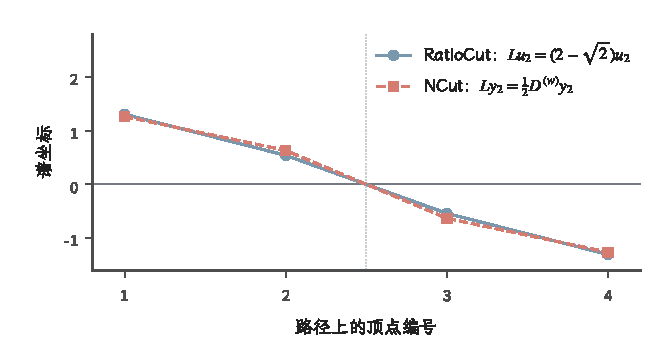
\includegraphics[width=\linewidth]{figures/math-preparation/reader-revision-graph/spectral-coordinates.pdf}
  \caption{单位边权路径\(1-2-3-4\)的两个精确谱方向。蓝实线为组合拉普拉斯的第二特征向量，红虚线为度加权广义特征向量；点形同时区分两者。为比较形状，图中两向量均按欧氏范数\(2\)缩放，此显示约定不改变各自的特征方程，也不替代NCut推导中的度加权范数。横轴只有四个顶点，连线仅引导阅读，竖虚线标出零阈值切分的位置。}
  \label{fig:graph-theory-spectral-coordinates}
\end{figure}

松弛向量不是离散分割本身。按符号或阈值切分会产生一个可行割，其目标值应回到原离散
目标计算。谱间隙小还意味着特征向量容易受扰动旋转；重复特征值时，稳定对象是特征子空间，
不是某个算法任意选出的单一基向量。

\subsection{图扩散与谱滤波}

平滑坐标描述一个静态信号，扩散则描述如何逐步减小相邻顶点的差异。
令每个顶点按邻居与自身的差值调整，即\(f_i'(t)=\sum_jw_{i,j}(f_j(t)-f_i(t))\)：
邻居较高就抬高本点，邻居较低就降低本点。把这些方程合在一起，正好得到负拉普拉斯作用。

连续时间图扩散定义为
\begin{equation}
  \frac{\mathrm{d}\bm{f}(t)}{\mathrm{d}t}
  =-\bm{L}\bm{f}(t),
  \qquad
  \bm{f}(0)=\bm{f}_0.
  \label{eq:graph-theory-heat-equation}
\end{equation}
第~\ref{chap:matrix-analysis}章的矩阵指数给出
\[
  \bm{f}(t)=\exp(-t\bm{L})\bm{f}_0
  =\sum_{k=1}^{n}e^{-t\lambda_k}
  \langle\bm{u}_k,\bm{f}_0\rangle\bm{u}_k.
\]
特征值大的模式衰减更快，零特征值对应的分量保持不变。正权支撑图连通时，
\(\bm{f}(t)\)趋向初始信号的常量投影；支撑图不连通时，每个支撑连通分量分别趋向
自己的平均。

总和保持来自\(\bm{1}^{\top}\bm{L}=\bm{0}^{\top}\)：
\[
  \frac{\mathrm{d}}{\mathrm{d}t}
  \bm{1}^{\top}\bm{f}(t)=0.
\]
平方范数与Dirichlet能量是两个不同的量。平方范数的导数恰好是负的Dirichlet能量：
\[
  \frac{\mathrm{d}}{\mathrm{d}t}
  \frac12\lVert\bm{f}(t)\rVert_2^2
  =
  -\bm{f}(t)^{\top}\bm{L}\bm{f}(t)
  \leq0.
\]
Dirichlet能量本身也下降，但对应的导数多出一个拉普拉斯：
\[
  \frac{\mathrm{d}}{\mathrm{d}t}
  \left[\bm{f}(t)^{\top}\bm{L}\bm{f}(t)\right]
  =
  -2\bm{f}(t)^{\top}\bm{L}^2\bm{f}(t)
  =
  -2\lVert\bm{L}\bm{f}(t)\rVert_2^2
  \leq0.
\]
第一个等式说明非平滑分量消耗平方范数，第二个等式直接说明边上平方差总量不会增加。
扩散因此削弱顶点间差异，但不表示它保留任务所需的类别边界。扩散时间过长会把同一
正权支撑连通分量内所有差异抹平。

在贯穿图上令每条边权为\(1\)，取\(\bm f_0=(1,0,0,0)^\top\)。其拉普拉斯特征值为\(0,2,4,4\)，因此不同频率的保留比例分别为\(1,e^{-2t},e^{-4t}\)。图~\ref{fig:graph-diffusion-spectrum}显示初始集中在顶点\(1\)的信号逐步分散；由于图连通且总和为\(1\)，极限为各顶点上的\(1/4\)，而不是信号全部消失。两个相同的特征值\(4\)对应不同特征向量，它们只是使用相同的衰减系数。

\begin{figure*}[htbp]
  \centering
  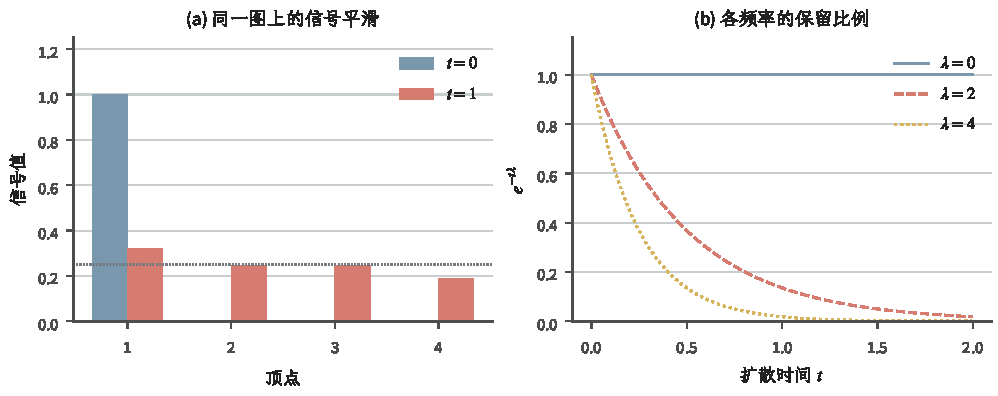
\includegraphics[width=\linewidth]{figures/math-preparation/probability-discrete/graph-diffusion-spectrum.pdf}
  \caption{贯穿四顶点图的解析式扩散。左图比较\(\bm f(0)=(1,0,0,0)^\top\)与\(\bm f(1)=e^{-\bm L}\bm f(0)\)，灰虚线为最终均值\(1/4\)；右图绘制三个不同特征值\(0,2,4\)的保留比例，特征值\(4\)实际具有重数\(2\)。柱与曲线由该图的拉普拉斯直接计算，不是仿真实验的均值或误差条。}
  \label{fig:graph-diffusion-spectrum}
\end{figure*}

\subsection{离散Dirichlet能量与连续极限}

式~\eqref{eq:graph-theory-dirichlet-energy}是第
~\ref{chap:differential-geometry-and-symmetry}章连续Dirichlet能量
\[
  \int_{\mathcal{M}}
  \lVert\operatorname{grad}f\rVert_g^2\,\mathrm{d}V_g
\]
的离散对应：连续梯度衡量无穷小方向的变化，图边差分只比较被连接的样本对。两者形式
相似，却不能只靠形式宣布收敛。

若图来自点云，邻域半径决定哪些局部方向被采样，核权重决定不同距离的贡献，归一化决定
是否保留采样密度，边界又会改变极限条件。邻域过大可能跨越弯曲流形的不同折，过小则使
图断连。样本密度不均时，未校正的图拉普拉斯可能逼近带密度漂移的算子，而不是纯粹由
Riemann体积定义的Laplace--Beltrami算子。

因此，图谱只相对于已经选定的图和权重给出精确代数结论。它是否近似某个连续空间，
需要额外的采样、尺度与归一化条件；它是否保留预测语义，又需要任务证据。

\section{在重编号下保持表示并比较图结构}
\label{sec:graph-theory-structure-comparison}

图的顶点编号可以任意改变。一个结构表示既要避免把编号差异当成结构差异，又需要区分真正不同的图。这是两个要求：等变或不变性解决前者，局部细化的区分能力关系到后者。下面先检验拉普拉斯和滤波器的置换行为，再以多重集合细化展示局部表示的能力边界。

\subsection{顶点置换与等变性}

顶点级输出和整图级输出需要不同的编号行为。例如预测每个顶点的数值，重新编号后预测也应随顶点重排，
这称为等变；判断整张图是否连通，重新编号后答案应保持相同，这称为不变。
这两个术语的完整定义见定义~\ref{def:geometry-equivariant-map}与定义~\ref{def:geometry-invariant-map}；这里把它们用于有限置换。

顶点名称只是坐标标签。同一图经置换矩阵\(\bm{P}\)重编号后，
\[
  \bm{W}'=\bm{P}\bm{W}\bm{P}^{\top},
  \qquad
  \bm{D}^{(w)\prime}=\bm{P}\bm{D}^{(w)}\bm{P}^{\top},
  \qquad
  \bm{L}'=\bm{P}\bm{L}\bm{P}^{\top}.
  \label{eq:graph-theory-laplacian-relabel}
\]
若顶点信号也重编号为\(\bm{f}'=\bm{P}\bm{f}\)，则
\[
  \bm{L}'\bm{f}'=\bm{P}\bm{L}\bm{f}.
\]
图拉普拉斯作用因此对顶点置换等变：输入顶点怎样重排，输出按同样方式重排。

更一般地，图滤波器若为多项式
\begin{equation}
  h(\bm{L})=\sum_{k=0}^{K}a_k\bm{L}^k,
  \label{eq:graph-theory-polynomial-filter}
\end{equation}
则
\[
  h(\bm{L}')\bm{f}'
  =\sum_{k=0}^{K}a_k(\bm{P}\bm{L}\bm{P}^{\top})^k\bm{P}\bm{f}
  =\bm{P}h(\bm{L})\bm{f},
\]
因为\(\bm{P}^{\top}\bm{P}=\bm{I}\)。若再对顶点输出作求和等对称汇总，可以得到置换
不变的图级表示。等变性只保证结果不依赖任意编号，不保证不同非同构图一定得到不同表示。

两张无向图\(\mathcal G=(V,E)\)与\(\mathcal G'=(V',E')\)若存在顶点双射\(\rho:V\to V'\)，使
\[
  \{i,j\}\in E\quad\Longleftrightarrow\quad\{\rho(i),\rho(j)\}\in E',
\]
就称为\term{同构}（isomorphic）。它表示忽略顶点名称后，连接关系完全相同；对有向图要保持有序弧的方向，
若比较加权图，还要保持对应边的权重。
无权图或所有结构边权均非零的加权图，可以等价地用置换矩阵条件
\(\bm A'=\bm P\bm A\bm P^\top\)判断同构。若允许零权结构边，则还必须核对边集或邻接掩码：
两顶点空图与含一条零权边的图都可以有\(\bm A=\bm0\)，却有不同连接结构。
即便矩阵足以确定结构，也不能用一般特征分解替代置换判据：同谱图可能不同构，重复特征值下特征向量基也不唯一。

\subsection{多重集合细化与局部结构}

与编号无关还不够：把每张图都映成同一个常数也满足不变性，却没有区分结构的能力。
一个更有信息的做法是反复比较每个顶点看到的邻域，把局部形态不同的顶点逐渐区分开。
为了不依赖邻居的排列顺序，同时保留某类邻居有多少个，需要使用多重集合。

邻居没有天然顺序，所以一个顶点的局部结构应通过邻居标记的
\term{多重集合}（multiset）表示。多重集合既记录元素种类，也记录每种元素出现次数；
\(\{a,a,b\}\)与\(\{a,b\}\)不同，但不区分排列次序。

\begin{definition}[一维邻域标记细化]
\label{def:graph-theory-wl-refinement}
一维Weisfeiler--Leman细化（1-dimensional Weisfeiler--Leman refinement,
1-WL）从初始标记\(c_i^{(0)}\)出发，反复令
\begin{equation}
  c_i^{(t+1)}=\operatorname{HASH}\left(
    c_i^{(t)},
    \left\{\!\left\{
      c_j^{(t)}:j\in N(i)
    \right\}\!\right\}
  \right),
  \label{eq:graph-theory-wl-refinement}
\end{equation}
其中\(\operatorname{HASH}\)对不同输入对给出不同新标记。每轮都把顶点自身旧标记与
邻居标记多重集组合。
\end{definition}

\(\operatorname{HASH}\)在这里是无碰撞编码的数学约定，不能直接假定一个普通有限哈希函数也绝不碰撞。
比较两张图时须使用一致的初始标记规则和同一编码对应；任意各自起名会使标记名称不可比较。
由于输入只包含自身标记与无序邻居计数，同构重编号只会同步重排标记，不改变各标记的出现次数。

这个过程会在有限步后稳定。令\(\mathcal{P}^{(t)}\)表示按
\(c_i^{(t)}\)相等关系得到的顶点分区。由于更新输入包含顶点自身旧标记，旧标记不同的
两个顶点下一轮仍不可能获得相同标记，所以
\(\mathcal{P}^{(t+1)}\)只能细分\(\mathcal{P}^{(t)}\)，不能合并其中的块。若分区
尚未稳定，块数至少增加\(1\)；而\(n\)个顶点至多分成\(n\)个非空块。因此从任意初始
分区出发，严格细分至多发生\(n-1\)次。某轮分区不再改变后，下一轮每个块中的顶点仍有
相同的自身标记和邻居标记计数，后续分区也保持不变。这里的“稳定”指等价类不再细分，
哈希实现仍可为这些类换用新的符号名称。

细化稳定不表示已经解决图同构。若所有顶点初始同标记，六顶点环\(C_6\)与两个互不相连
的三角形都让每个顶点始终看到两个同标记邻居；1-WL无法区分二者，尽管一张图连通、另一张
不连通。若把任意顶点编号当作固定初始特征，结果就会依赖编号，不能作为这个无标记图比较问题的无条件补救。
额外顶点属性若随置换同步移动，算法仍可等变，但输入已改成带属性图；那是另一个比较设定。

\begin{figure}[htbp]
  \centering
  \begingroup
\input{figures/math-preparation/reader-revision-graph/diagram-style}
\begin{tikzpicture}[text=FigureInk]
  \node[reader label] at (0,1.7) {(a) 六顶点环 \(C_6\)};
  \foreach \i in {1,...,6}
    \node[reader vertex,fill=FigureYellowFill] (a\i) at ({90-60*(\i-1)}:1.1) {};
  \foreach \i/\j in {1/2,2/3,3/4,4/5,5/6,6/1}
    \draw[reader edge] (a\i)--(a\j);
  \node[reader label] at (5.2,1.7) {(b) 两个不相交三角形};
  \foreach \x/\prefix in {3.8/b,6.6/c}
  {
    \node[reader vertex,fill=FigureYellowFill] (\prefix1) at (\x,0.9) {};
    \node[reader vertex,fill=FigureYellowFill] (\prefix2) at (\x-0.75,-0.6) {};
    \node[reader vertex,fill=FigureYellowFill] (\prefix3) at (\x+0.75,-0.6) {};
    \draw[reader edge] (\prefix1)--(\prefix2)--(\prefix3)--(\prefix1);
  }
  \node[reader label] at (0,-1.85) {每个顶点：2个同标记邻居};
  \node[reader label] at (5.2,-1.85) {每个顶点：2个同标记邻居};
\end{tikzpicture}
\endgroup

  \caption{相同局部计数不保证相同整体结构。所有顶点从同一标记开始，每轮都看见两个同标记邻居，因此两张六顶点图的1-WL标记计数始终相同。左图只有一个连通分量，右图有两个；这证明该局部细化不能在这个例子中识别连通性的差异，而不是说连通性本身难以计算。浅黄填充只表示同标记，圆内不放唯一编号，以免改变例子的输入。}
  \label{fig:graph-theory-wl-local-ambiguity}
\end{figure}

1-WL提供的是局部组合表达的参照。使用共享顶点更新和对称邻域聚合的具体图网络能否达到、
低于或超过该区分能力，要在模型正文中根据聚合函数、初始特征和读出方式证明。本章只建立
多重集合、置换作用和细化过程，不把结构等变性升级成学习能力或泛化保证。

\section{本章小结}
\label{sec:graph-theory-summary}

图的第一个作用是保留关系的结构，表示方式必须与查询相匹配。普通边、带方向的弧和高阶因子的作用域保留的信息不同，不能把一张关系图自动解释成概率或因果模型。
条件独立查询还会随条件集合改变：祖先道德化为每个DAG查询提供无向判据，但只有满足完美性与弦图条件时，才存在保存全部分离答案的固定等价表示。

图的第二个作用是组织计算。先明确要求总权重、边缘量还是最优配置，再选择组合与汇总运算，消元才有确定含义。
分配律保证汇总内部变量时保留原查询，分隔集和树分解则限制中间表的依赖范围。
贯穿例先处理顶点\(1,4\)只需宽度\(2\)，先处理顶点\(2\)却产生填充边\(\{1,4\}\)和宽度\(3\)。
弦图刻画无需补边的完美消元序，树宽衡量能达到的最小袋宽度；两者都不取代对取值域、因子成本和查询运算次序的检查。
针对特殊目标，还可以利用更强结构：非负边长支持Dijkstra的贪心确定，割性质支持最小生成树，容量与守恒使最大流和最小割构成同值证书，二部匹配借助整数流完成配对，二值次模能量则能写成非负割容量。
这些保证各自服务于不同目标，不能仅凭图的外形选择算法。精确结构不足时，可行解与松弛下界共同说明当前答案离最优至多有多远。

图的第三个作用是构造信号与结构表示。拉普拉斯能量度量沿边的变化，谱松弛把离散分割转成实数坐标，扩散按特征值衰减非平滑成分。
RatioCut按顶点数平衡，NCut按加权体积平衡，所以两者的特征方程不同；连续极限还依赖图构造、采样密度、尺度与边界。
置换等变性保证顶点级输出随重编号同步变化，不变性保证整图输出不受编号影响，二者都不保证表示足够丰富。
六环与两个三角形的1-WL反例表明：正确的对称性和相同局部计数仍可能遗漏整体差异。

读者据此可以把一个图问题分成具体判断：表示是否保留所需关系，查询采用何种运算，结构能否缩小计算规模，以及输出是否有相应的正确性或误差证书。
第~\ref{chap:signal-analysis}章转向有顺序的信号，比较规则序列频率与这里的图频率，再把线性递推展开成随时间组织的状态核。


\bookpart{动力系统、控制与决策}{Dynamical Systems, Control and Decision}
\label{part:dynamical-systems-control-and-decision}

\chapter{信号分析}
\label{chap:signal-analysis}

第~\ref{chap:graph-theory}章刚把局部关系写成图，并用图拉普拉斯谱描述节点信号的
变化模式。更早的线性代数把矩阵理解为线性映射，矩阵分析又说明了怎样用谱坐标观察算子。
当输入带有时间、空间位置等顺序时，还会出现一类额外结构：同一个局部作用可以沿位置
重复使用。直接把这种作用写成一般矩阵当然可行，但那会隐藏重复的系数，也无法立即看出
边界、频率和采样怎样改变结果。

本章以两个有限序列
\begin{equation}
  \bm{x}=(1,2,1),\qquad
  \bm{h}=(1,-1)
  \label{eq:signal-analysis-running-example}
\end{equation}
作为贯穿例子。我们先从平移不变的线性滤波推出卷积，再把序列系数写成多项式；
复指数提供另一组坐标，使循环卷积化为逐点乘法。快速傅里叶变换、Toom--Cook和
Winograd类算法都利用“先改变表示、再做较少乘法、最后恢复结果”的思路，但它们
使用的分解并不相同。采样部分说明什么时候这种表示仍保留原信号，图信号和状态核则
把规则序列上的结论分别推广到不规则关系和递推系统。

\section{离散信号与线性滤波}
\label{sec:signal-analysis-discrete-filtering}

\subsection{信号是带索引的数值对象}

\term{离散时间信号}（discrete-time signal）是从整数索引到实数或复数的函数，
\[
  x:\mathbb{Z}\to\mathbb{C},\qquad t\mapsto x[t].
\]
索引$t$可以表示时间，也可以表示一维空间位置。信号的含义来自索引顺序，而不只是
一组数值：交换$x[0]$与$x[1]$通常会改变局部变化和滤波输出。若只有有限多个位置
非零，就称信号具有有限支撑。式~\eqref{eq:signal-analysis-running-example}中的
$\bm{x}$表示$x[0]=1,x[1]=2,x[2]=1$，其余位置取零；$\bm{h}$也作同样的零延拓。

对整数$r$，定义平移算子
\[
  (T_r x)[t]=x[t-r].
\]
$r>0$时，原来位于$t$的值移动到$t+r$。这个符号约定很重要，因为另一种常见约定
$x[t+r]$会把平移方向反过来。单位脉冲
\[
  \delta[t]=
  \begin{cases}
    1,&t=0,\\
    0,&t\neq0
  \end{cases}
\]
满足$T_r\delta[t]=\delta[t-r]$。任意有限支撑信号都可分解为平移脉冲之和：
\begin{equation}
  x[t]=\sum_{r\in\mathbb{Z}}x[r]\delta[t-r].
  \label{eq:signal-analysis-impulse-expansion}
\end{equation}
对每个固定$t$，只有$r=t$的一项非零。这个简单分解将把一般输入的响应归结为系统对
单个脉冲的响应。

\subsection{线性与平移不变共同推出卷积}

一个离散系统$\mathcal{H}$把输入信号$x$映射为输出信号$y=\mathcal{H}x$。
若对任意标量$a,b$及输入$x,z$都有
\[
  \mathcal{H}(ax+bz)=a\mathcal{H}x+b\mathcal{H}z,
\]
就称系统为线性的。若
\[
  \mathcal{H}(T_r x)=T_r(\mathcal{H}x)
  \qquad\text{对每个 }r\in\mathbb{Z}\text{成立},
\]
就称系统具有\term{平移不变性}（shift invariance）。这表示输入整体移动后，
输出只作同样移动，系统在不同位置使用同一规则。

令$h=\mathcal{H}\delta$，称$h$为系统的\term{脉冲响应}（impulse response）。
若$x$具有有限支撑，式~\eqref{eq:signal-analysis-impulse-expansion}是有限和，
线性性足以把$\mathcal{H}$移入求和。对无穷序列，记
\[
  \ell_1(\mathbb{Z})
  =
  \left\{
    x:\mathbb{Z}\to\mathbb{C}
    \,\middle|\,
    \sum_{t\in\mathbb{Z}}|x[t]|<\infty
  \right\},
  \qquad
  \lVert x\rVert_1=\sum_{t\in\mathbb{Z}}|x[t]|.
\]
也就是说，$\ell_1(\mathbb{Z})$由绝对可和序列组成。对一般的
$x\in\ell_1(\mathbb{Z})$，还需假设
$\mathcal{H}:\ell_1(\mathbb{Z})\to\ell_1(\mathbb{Z})$是有界线性且平移不变的
算子；这里有界表示存在与$x$无关的常数$C$，使
\[
  \lVert\mathcal{H}x\rVert_1\leq C\lVert x\rVert_1.
\]
令
\[
  x^{(N)}=\sum_{|r|\leq N}x[r]T_r\delta,
\]
则$x^{(N)}\to x$在$\ell_1$范数下成立；有界性蕴含连续性，因而
$\mathcal{H}x^{(N)}\to\mathcal{H}x$。同时
$h=\mathcal{H}\delta\in\ell_1(\mathbb{Z})$，而且
\[
  \sum_{t\in\mathbb{Z}}\sum_{r\in\mathbb{Z}}
  |x[r]h[t-r]|
  =
  \lVert x\rVert_1\lVert h\rVert_1
  <\infty,
\]
所以下面的无穷和绝对收敛。于是，
有限支撑情形直接由线性性得到、$\ell_1$情形通过上述极限得到
\begin{align}
  (\mathcal{H}x)[t]
  &=
  \mathcal{H}\left(\sum_{r\in\mathbb{Z}}x[r]T_r\delta\right)[t]
  \notag\\
  &=
  \sum_{r\in\mathbb{Z}}x[r](T_rh)[t]
  =
  \sum_{r\in\mathbb{Z}}x[r]h[t-r].
  \label{eq:signal-analysis-lti-convolution}
\end{align}

式~\eqref{eq:signal-analysis-lti-convolution}定义\term{离散卷积}
（discrete convolution），记为
\begin{equation}
  (x*h)[t]=\sum_{r\in\mathbb{Z}}x[r]h[t-r].
  \label{eq:signal-analysis-linear-convolution}
\end{equation}
核索引$t-r$随$r$增加而反向读取，这个翻转是数学卷积定义的一部分。卷积满足交换律；
令$s=t-r$便有
\[
  \sum_r x[r]h[t-r]
  =
  \sum_s h[s]x[t-s]
  =
  (h*x)[t].
\]
在绝对可和等允许交换求和次序的条件下，它还满足结合律和分配律。

\subsection{相关与卷积只差一个方向，却回答不同问题}

\term{互相关}（cross-correlation）常写为
\begin{equation}
  (x\star h)[t]
  =
  \sum_{r\in\mathbb{Z}}x[t+r]\overline{h[r]}.
  \label{eq:signal-analysis-cross-correlation}
\end{equation}
它把$h$按原方向滑过$x$，并在复数情形取共轭；上划线表示保持实部不变、把虚部
符号反转。若定义
$\widetilde{h}[r]=\overline{h[-r]}$，则
\[
  (x\star h)[t]=(x*\widetilde{h})[t].
\]
因此相关可以用卷积实现，但二者的核含义不同。信号处理中，相关常用于比较一个模板与
不同位置的局部片段；许多神经网络库把不翻转核的相关运算称为“卷积”。只要训练和
推理始终采用同一约定，参数可以适应该方向；在手算、复用滤波器或推导伴随算子时，
仍必须明确是否翻转以及是否取共轭。

\subsection{线性卷积与循环卷积采用不同边界}

设$x$的支撑为$0,\ldots,m-1$，$h$的支撑为$0,\ldots,r-1$。零延拓下的线性卷积
只可能在$0,\ldots,m+r-2$非零，因此完整输出长度为$m+r-1$。对贯穿例，
\begin{align*}
  (x*h)[0]&=1,\\
  (x*h)[1]&=2-1=1,\\
  (x*h)[2]&=1-2=-1,\\
  (x*h)[3]&=-1.
\end{align*}
所以
\begin{equation}
  \bm{x}*\bm{h}=(1,1,-1,-1).
  \label{eq:signal-analysis-running-linear-convolution}
\end{equation}
核$(1,-1)$在这里计算当前值减去前一个值；开头和末尾的结果还包含零延拓带来的边界
跳变。

若信号被视为长度$N$的周期序列，索引应按模$N$回绕。长度$N$的
\term{循环卷积}（circular convolution）定义为
\begin{equation}
  (x*_N h)[t]
  =
  \sum_{r=0}^{N-1}x[r]h[(t-r)\bmod N],
  \qquad t=0,\ldots,N-1.
  \label{eq:signal-analysis-circular-convolution}
\end{equation}
把例中的$\bm{h}$补成$(1,-1,0)$并取$N=3$，可得
\[
  \bm{x}*_3\bm{h}=(0,1,-1).
\]
它等于把式~\eqref{eq:signal-analysis-running-linear-convolution}中索引相差$3$
的项相加：首项$1$与末项$-1$叠在一起。循环边界不是零边界的近似，而是另一个线性
算子。

固定有限长度后，线性卷积可写成Toeplitz矩阵乘法，循环卷积可写成循环矩阵乘法。
例如
\[
  \begin{bmatrix}
    1&0&0\\
    -1&1&0\\
    0&-1&1\\
    0&0&-1
  \end{bmatrix}
  \begin{bmatrix}1\\2\\1\end{bmatrix}
  =
  \begin{bmatrix}1\\1\\-1\\-1\end{bmatrix}.
\]
矩阵的重复对角线来自参数共享。裁剪为“valid”输出、补零后保持输入长度，或使用反射、
复制等边界，都会改变矩阵的首尾行。平移不变性在无限网格或循环群上最为精确；
有限区间上的边界处理通常会破坏全局平移不变性。

“valid”并不是另一种卷积定义，而是只保留核完全落在已知输入区间内的输出。按本章
$h[0],\ldots,h[r-1]$的因果索引约定，当$m\geq r$时，这些输出对应
$t=r-1,\ldots,m-1$，共$m-r+1$项；若$m<r$，则没有这样的输出。补零得到的首尾
输出仍有定义，但它们使用了人为指定的区间外数值。因而比较两个实现时，除了核系数，
还要同时核对延拓方式、保留的输出索引和核的方向。

\section{多项式乘法、求值与余数}
\label{sec:signal-analysis-polynomial-arithmetic}

\subsection{卷积系数就是多项式乘积系数}

有限序列可以用形式多项式编码。对
\[
  \bm{x}=(x_0,\ldots,x_{m-1}),\qquad
  \bm{h}=(h_0,\ldots,h_{r-1}),
\]
定义
\[
  X(z)=\sum_{i=0}^{m-1}x_i z^i,\qquad
  H(z)=\sum_{j=0}^{r-1}h_j z^j.
\]
变量$z$在这里首先是记录索引的形式符号。乘积为
\begin{align}
  X(z)H(z)
  &=
  \sum_{i=0}^{m-1}\sum_{j=0}^{r-1}x_i h_jz^{i+j}
  \notag\\
  &=
  \sum_{t=0}^{m+r-2}
  \left(\sum_{i+j=t}x_i h_j\right)z^t.
  \label{eq:signal-analysis-polynomial-convolution}
\end{align}
括号中的系数正是$(x*h)[t]$。卷积的交换律和结合律也可分别从多项式乘法的交换律和
结合律得到。

贯穿例对应
\[
  X(z)=1+2z+z^2,\qquad H(z)=1-z,
\]
因而
\begin{equation}
  P(z)=X(z)H(z)=1+z-z^2-z^3.
  \label{eq:signal-analysis-running-polynomial-product}
\end{equation}
其四个系数与式~\eqref{eq:signal-analysis-running-linear-convolution}完全一致。
这种对应没有减少计算，只是把“哪些下标相加”改写成“哪些幂次相乘”。真正的计算收益
来自下一步：多项式除了系数表示，还可以用函数值或余数表示。

\subsection{求值与插值是同一多项式的另一组坐标}

次数小于$L$的多项式空间维数为$L$。选取$L$个两两不同的数
$a_0,\ldots,a_{L-1}$，求值映射
\[
  E(P)=\bigl(P(a_0),\ldots,P(a_{L-1})\bigr)
\]
是一个线性映射。若$E(P)=\bm{0}$，则$P$有$L$个不同根；次数小于$L$的非零
多项式至多有$L-1$个根，所以只能有$P=0$。求值映射是同维有限空间之间的单射，
因而可逆。其逆就是\term{多项式插值}（polynomial interpolation）。

具体地，Lagrange基多项式
\[
  \ell_j(z)=
  \prod_{\substack{0\leq k<L\\k\neq j}}
  \frac{z-a_k}{a_j-a_k}
\]
满足$\ell_j(a_k)=\delta_{j,k}$。因此
\begin{equation}
  P(z)=\sum_{j=0}^{L-1}P(a_j)\ell_j(z),
  \qquad \deg P<L.
  \label{eq:signal-analysis-lagrange-interpolation}
\end{equation}
若要计算$P=XH$，可以先分别求$X(a_j)$与$H(a_j)$，再用
$P(a_j)=X(a_j)H(a_j)$逐点相乘，最后插值。逐点乘法数是$L$，代价被转移到求值
与插值中的线性组合。选点、问题规模和数值精度决定这种交换是否值得。

\subsection{带余除法把高次信息压到指定模中}

求值是余数的一种特殊情形。为建立更一般的表示，先考虑多项式除法。

\begin{theorem}[多项式带余除法]
\label{thm:signal-analysis-polynomial-division}
设$F$为一个域，$A(z),M(z)\in F[z]$且$M\neq0$。存在唯一的多项式
$Q(z),R(z)$使
\[
  A(z)=Q(z)M(z)+R(z),
  \qquad \deg R<\deg M.
\]
\end{theorem}

\begin{proof}
若$\deg A<\deg M$，取$Q=0,R=A$即可。否则设$A$与$M$的最高次项分别为
$a_pz^p$与$m_qz^q$，其中$p\geq q$。因为$F$是域，$m_q$可逆；从$A$中减去
$(a_p/m_q)z^{p-q}M$便消去最高次项。重复此过程，次数严格下降，有限步后得到次数
小于$\deg M$的余数。

若另有$A=Q'M+R'$且$\deg R',\deg R<\deg M$，则
$(Q-Q')M=R'-R$。左侧若非零，次数至少为$\deg M$；右侧若非零，次数小于
$\deg M$，矛盾。因此$Q=Q'$且$R=R'$。
\end{proof}

带余除法还给出后文重构所需的互素判据。对非零多项式$A,B$反复作
\[
  A=Q_0B+R_1,\qquad
  B=Q_1R_1+R_2,\qquad \ldots
\]
每个非零余数的次数都严格下降，所以过程有限步终止；最后一个非零余数经过首项归一化，
就是$A,B$的\term{最大公因式}（greatest common divisor）。从最后一个等式向前
回代，每个余数都能写成$A,B$的多项式线性组合。因此存在$U,V\in F[z]$使
\begin{equation}
  U(z)A(z)+V(z)B(z)=\gcd(A,B).
  \label{eq:signal-analysis-polynomial-bezout}
\end{equation}
这就是多项式的Bézout恒等式。特别地，$A,B$互素当且仅当可找到$U,V$使左侧等于
$1$；“互素”在这里表示最大公因式为非零常数。

例如
\[
  z^2+1=(z+1)(z-1)+2,
\]
所以$z-1$与$z^2+1$互素，而且回代立即给出
\[
  1=\frac{1}{2}(z^2+1)-\frac{1}{2}(z+1)(z-1).
\]
后文构造中国剩余重构系数时，使用的正是这一步，而不是假设逆元凭空存在。

余数记为$A\bmod M$，并把相差$M$倍数的多项式视为同一个
\term{剩余类}（residue class）。当$M(z)=z-a$时，带余除法给出
\[
  A(z)=Q(z)(z-a)+A(a),
\]
所以关于一次多项式$z-a$的余数就是点值$A(a)$。

模多项式还编码边界。因为在模$z^N-1$的剩余类中有$z^N=1$，
$z^{N+s}$与$z^s$的系数会合并。于是
\begin{equation}
  \left(X(z)H(z)\right)\bmod(z^N-1)
  =
  \sum_{t=0}^{N-1}(x*_Nh)[t]z^t.
  \label{eq:signal-analysis-polynomial-circular-convolution}
\end{equation}
线性卷积与循环卷积的差别由此变成“保留普通乘积”还是“再对$z^N-1$取模”。
若$\deg(XH)<N$，取模不会合并任何系数，两种卷积在补零后的前$N$项相同；
若次数达到$N$，高次项就会回绕。

\section{复指数与频率表示}
\label{sec:signal-analysis-frequency-representation}

\subsection{复指数把平移变成相位乘法}

后文会同时使用复数、复向量和复矩阵。记$\mathrm{i}^2=-1$；对
$z=a+\mathrm{i}b$，其\term{复共轭}（complex conjugate）与模长分别为
\[
  \overline z=a-\mathrm{i}b,
  \qquad
  |z|=\sqrt{z\overline z}.
\]
当$z\neq0$时，可写成$z=|z|e^{\mathrm{i}\arg z}$，其中$\arg z$是相角。
互相关式~\eqref{eq:signal-analysis-cross-correlation}中的上划线也表示复共轭。
对$\bm{u},\bm{v}\in\mathbb{C}^N$，本章采用复内积
\[
  \langle\bm{u},\bm{v}\rangle
  =
  \sum_{t=0}^{N-1}u[t]\overline{v[t]}.
\]
在第二个变量上取共轭使
$\langle\bm{u},\bm{u}\rangle=\sum_t|u[t]|^2$为非负实数。复矩阵
$\bm{A}$的\term{共轭转置}（conjugate transpose）记为
$\bm{A}^*=\overline{\bm{A}}^{\top}$；若$\bm{A}^*\bm{A}=\bm{I}$，则称
$\bm{A}$为酉矩阵。

时域中的平移会改动许多坐标。复指数
\[
  \phi_{\omega}[t]=e^{\mathrm{i}\omega t}
\]
却在平移后只差一个标量：
\[
  (T_r\phi_{\omega})[t]
  =
  e^{\mathrm{i}\omega(t-r)}
  =
  e^{-\mathrm{i}\omega r}\phi_{\omega}[t].
\]
因此复指数是平移算子的特征函数，频率$\omega$标记不同的特征模式，系数
$e^{-\mathrm{i}\omega r}$记录平移产生的相位变化。这解释了频率表示为何适合分析
平移不变系统：所有平移共享同一组模式。

\subsection{离散傅里叶变换建立有限维正交坐标}

对长度$N$的序列，令
\[
  \omega_N=e^{-2\pi\mathrm{i}/N}.
\]
\term{离散傅里叶变换}（discrete Fourier transform, DFT）及逆变换定义为
\begin{align}
  \widehat{x}[k]
  &=
  \sum_{t=0}^{N-1}x[t]\omega_N^{kt},
  &&k=0,\ldots,N-1,
  \label{eq:signal-analysis-dft}\\
  x[t]
  &=
  \frac{1}{N}\sum_{k=0}^{N-1}
  \widehat{x}[k]\omega_N^{-kt},
  &&t=0,\ldots,N-1.
  \label{eq:signal-analysis-idft}
\end{align}
正变换也就是在$N$次单位根$1,\omega_N,\ldots,\omega_N^{N-1}$处计算多项式
$X(z)$的值。它既是频率坐标，也是第~\ref{sec:signal-analysis-polynomial-arithmetic}
节求值表示的一种特殊选点。

逆变换来自单位根的正交关系。对整数$t,s$，
\begin{equation}
  \sum_{k=0}^{N-1}\omega_N^{k(t-s)}
  =
  \begin{cases}
    N,&t\equiv s\pmod N,\\
    0,&t\not\equiv s\pmod N.
  \end{cases}
  \label{eq:signal-analysis-root-orthogonality}
\end{equation}
第一种情形每项都是$1$。第二种情形令$q=\omega_N^{t-s}\neq1$，利用$q^N=1$，
几何级数之和为$(1-q^N)/(1-q)=0$。把式~\eqref{eq:signal-analysis-dft}
代入式~\eqref{eq:signal-analysis-idft}，再交换两个有限求和，只有$s=t$的项留下，
从而恢复$x[t]$。这也证明DFT没有丢失长度$N$序列的信息。

若把DFT矩阵记为$\bm{F}$，其中$F_{k,t}=\omega_N^{kt}$，则
\[
  \bm{F}^{*}\bm{F}=N\bm{I}.
\]
因此$\bm{F}/\sqrt{N}$是酉矩阵。第~\ref{chap:matrix-analysis}章的谱语言在这里
给出一个直接解释：$\bm{F}/\sqrt{N}$才是保持二范数的正交坐标变换。本章定义的
未归一化DFT满足
$\lVert\widehat{\bm{x}}\rVert_2=\sqrt{N}\lVert\bm{x}\rVert_2$，
逆变换中的$1/N$会补回这一尺度。

\subsection{幅度、相位与实信号的共轭对称}

每个非零复系数都可写成
\[
  \widehat{x}[k]=
  |\widehat{x}[k]|e^{\mathrm{i}\arg\widehat{x}[k]}.
\]
模长描述该频率坐标的大小，相角描述它相对于所选时间原点的相位。若把信号循环平移$r$
个位置，DFT变为
\[
  \widehat{T_rx}[k]
  =
  \omega_N^{kr}\widehat{x}[k].
\]
幅度不变，相位随$k$线性改变。仅保留幅度会丢失位置信息；两个具有相同幅度谱的信号
不必具有相同波形。

若$x[t]$为实数，则
\begin{align*}
  \overline{\widehat{x}[k]}
  &=
  \sum_{t=0}^{N-1}x[t]\omega_N^{-kt}\\
  &=
  \sum_{t=0}^{N-1}x[t]\omega_N^{(N-k)t}
  =
  \widehat{x}[(N-k)\bmod N].
\end{align*}
这称为\term{共轭对称}（conjugate symmetry）。频率$0$总是实数；$N$为偶数时，
$k=N/2$对应的Nyquist频率也为实数。其余频率成共轭对出现，所以实信号的完整复频谱
包含冗余，但直接丢弃一半频率时仍要保留正确的缩放和端点约定。

\subsection{Parseval关系说明能量只是在坐标间重排}

由$\bm{F}^{*}\bm{F}=N\bm{I}$，
\[
  \lVert\widehat{\bm{x}}\rVert_2^2
  =
  \bm{x}^{*}\bm{F}^{*}\bm{F}\bm{x}
  =
  N\lVert\bm{x}\rVert_2^2.
\]
于是得到离散的\term{Parseval关系}
\begin{equation}
  \sum_{t=0}^{N-1}|x[t]|^2
  =
  \frac{1}{N}\sum_{k=0}^{N-1}
  |\widehat{x}[k]|^2.
  \label{eq:signal-analysis-parseval}
\end{equation}
这里的$1/N$来自本章把归一化全部放在逆变换中。若正逆变换各用$1/\sqrt{N}$，
等式两侧便没有额外因子。比较不同资料中的频谱数值前，必须先核对变换的符号与归一化
约定。

\subsection{连续周期信号需要区分收敛方式}

有限维DFT只涉及有限求和，不存在无穷级数的收敛问题。把同一正交展开思路推广到
连续周期信号后，才需要区分平方平均收敛与逐点收敛。对周期为$T$的平方可积连续信号
$f(t)$，复指数$e^{\mathrm{i}2\pi kt/T}$在内积
\[
  \langle f,g\rangle
  =
  \frac{1}{T}\int_0^T f(t)\overline{g(t)}\,\mathrm{d}t
\]
下正交。其\term{傅里叶系数}（Fourier coefficient）为
\[
  c_k=
  \frac{1}{T}\int_0^T
  f(t)e^{-\mathrm{i}2\pi kt/T}\,\mathrm{d}t.
\]
形式上，傅里叶级数写为
\begin{equation}
  f(t)\sim\sum_{k\in\mathbb{Z}}c_k
  e^{\mathrm{i}2\pi kt/T}.
  \label{eq:signal-analysis-fourier-series}
\end{equation}
若只假设$f\in L^2[0,T]$，等号应理解为平方平均意义下收敛；逐点收敛还需要额外
规则性，并且跳跃点处通常收敛到左右极限的平均。频率展开不是无条件的逐点恒等式。
在相同归一化下，连续周期信号还满足Parseval关系
\begin{equation}
  \frac{1}{T}\int_0^T|f(t)|^2\,\mathrm{d}t
  =
  \sum_{k\in\mathbb{Z}}|c_k|^2.
  \label{eq:signal-analysis-continuous-parseval}
\end{equation}
它是$L^2$中的能量恒等式，不要求傅里叶级数在每一点都等于$f$。

一个具体边界例子是周期为$2\pi$的方波：在$0<t<\pi$取$1$，在
$-\pi<t<0$取$-1$，再作周期延拓。直接积分得到$c_0=0$，偶数$k$对应
$c_k=0$，奇数$k$对应
\[
  c_k=\frac{2}{\pi\mathrm{i}k}.
\]
方波在除跳跃点外的每个连续点由级数恢复，在跳跃点则收敛到左右极限的平均$0$；
与此同时，式~\eqref{eq:signal-analysis-continuous-parseval}仍在$L^2$意义下成立。
这一区别说明，平均平方误差趋于零并不能逐点排除跳跃附近的振荡。

\section{卷积定理与快速变换}
\label{sec:signal-analysis-fast-transforms}

\subsection{循环卷积在频域中逐点相乘}

\begin{theorem}[离散循环卷积定理]
\label{thm:signal-analysis-circular-convolution-theorem}
设$x,h$为长度$N$的复序列，DFT采用
式~\eqref{eq:signal-analysis-dft}的约定，则
\[
  \widehat{x*_Nh}[k]
  =
  \widehat{x}[k]\widehat{h}[k],
  \qquad k=0,\ldots,N-1.
\]
\end{theorem}

\begin{proof}
从定义出发，并把$a=(t-r)\bmod N$作为新的求和索引：
\begin{align*}
  \widehat{x*_Nh}[k]
  &=
  \sum_{t=0}^{N-1}
  \sum_{r=0}^{N-1}
  x[r]h[(t-r)\bmod N]\omega_N^{kt}\\
  &=
  \sum_{r=0}^{N-1}
  \sum_{a=0}^{N-1}
  x[r]h[a]\omega_N^{k(r+a)}\\
  &=
  \left(\sum_{r=0}^{N-1}x[r]\omega_N^{kr}\right)
  \left(\sum_{a=0}^{N-1}h[a]\omega_N^{ka}\right).
\end{align*}
第二个等号中，$t$遍历一个完整剩余类时$a$也恰好遍历$0,\ldots,N-1$；
即使$t$与$r+a$相差$N$的整数倍，$\omega_N^{kN}=1$也保证幂值不变。最后两项
分别是$\widehat{x}[k]$和$\widehat{h}[k]$。
\end{proof}

因此
\begin{equation}
  x*_Nh
  =
  \mathcal{F}_N^{-1}
  \left(
    \mathcal{F}_N(x)\odot\mathcal{F}_N(h)
  \right).
  \label{eq:signal-analysis-frequency-domain-convolution}
\end{equation}
循环卷积矩阵由DFT基对角化，每个频率上的“特征值”就是核的DFT系数。这个结论同时
连接了第~\ref{chap:matrix-analysis}章的谱分解和本章的多项式求值：循环矩阵、
模$z^N-1$的乘法与单位根求值
描述的是同一个算子。

若要得到长度$m+r-1$的线性卷积，必须把两个序列都补零到
\begin{equation}
  N\geq m+r-1.
  \label{eq:signal-analysis-linear-padding-condition}
\end{equation}
此时乘积次数小于$N$，模$z^N-1$不会发生系数回绕。只把两者补到
$N\geq\max(m,r)$不够；它保证输入装得下，却未保证乘积装得下。

\subsection{FFT利用单位根的递归结构}

直接计算$N$个DFT系数，每个需要$N$项求和，运算量为$O(N^2)$。
\term{快速傅里叶变换}（fast Fourier transform, FFT）不是另一种变换，而是一族
利用求值点结构快速计算DFT的算法\scite{cooley1965fft}以$N$为偶数的基二
Cooley--Tukey分解为例，
将输入的偶数项与奇数项分别组成
\[
  x_{\mathrm{e}}[r]=x[2r],\qquad
  x_{\mathrm{o}}[r]=x[2r+1].
\]
记它们的长度$N/2$ DFT为$E[k]$和$O[k]$。因为$\omega_N^2=\omega_{N/2}$，
对$0\leq k<N/2$有
\begin{align}
  \widehat{x}[k]
  &=
  E[k]+\omega_N^kO[k],
  \notag\\
  \widehat{x}[k+N/2]
  &=
  E[k]-\omega_N^kO[k].
  \label{eq:signal-analysis-fft-butterfly}
\end{align}
第二式利用了$\omega_N^{N/2}=-1$。两个较小DFT的同一对结果通过一次加法和一次
减法产生两个频率，并没有舍弃后一半频率。

当$N=2^q$时，递推
\[
  T(N)=2T(N/2)+O(N)
\]
给出$T(N)=O(N\log N)$。其他合数长度可按不同因子分解，质数长度也有相应算法；
“使用FFT”不等于必须补到二的幂。补到更方便的长度可能降低实现常数，也可能增加
无用频点和存储，需按具体规模判断。

对贯穿例补零到$N=4$：
\[
  \bm{x}_4=(1,2,1,0),\qquad
  \bm{h}_4=(1,-1,0,0).
\]
对$\bm{x}_4$，偶数分支$(1,1)$的二点DFT为$(2,0)$，奇数分支$(2,0)$的
二点DFT为$(2,2)$。取$\omega_4=-\mathrm{i}$并按
式~\eqref{eq:signal-analysis-fft-butterfly}合并，得到
\[
  (2+2,\ 0-2\mathrm{i},\ 2-2,\ 0+2\mathrm{i})
  =
  (4,-2\mathrm{i},0,2\mathrm{i}).
\]
同理，$\bm{h}_4$的偶、奇分支DFT分别为$(1,1)$与$(-1,-1)$，蝶形合并得到
$(0,1+\mathrm{i},2,1-\mathrm{i})$。这一步显示四点结果如何由两个二点变换复用，
而不只是直接代入DFT定义。

在$1,-\mathrm{i},-1,\mathrm{i}$四个单位根处，
\[
  \widehat{\bm{x}}_4=(4,-2\mathrm{i},0,2\mathrm{i}),\qquad
  \widehat{\bm{h}}_4=(0,1+\mathrm{i},2,1-\mathrm{i}).
\]
例如逆变换的四个分子依次为
\[
  4-2\mathrm{i}+2\mathrm{i},\quad
  4+2+2,\quad
  4+2\mathrm{i}-2\mathrm{i},\quad
  4-2-2,
\]
除以$4$后恢复$(1,2,1,0)$。这一步同时核对了频率顺序、指数符号和$1/N$归一化，
任何一项约定改变都要相应修改逆变换。

逐点乘积为
\[
  (0,2-2\mathrm{i},0,2+2\mathrm{i}),
\]
逆DFT恢复$(1,1,-1,-1)$。若只用$N=3$，末项会回绕到首项，得到的便是
$(0,1,-1)$而非线性卷积。

\subsection{Toom--Cook用一般求值点减少系数乘法}

Toom--Cook方法把多项式分块，选择足够多的求值点，逐点相乘后再插值。对本例的
二次多项式$X$与一次多项式$H$，乘积次数至多为$3$，可使用
$0,1,-1,\infty$四个点；其中“在$\infty$处求值”只表示读取最高次项系数，
并非把无穷大传给数值程序\scite{math-knuth1997seminumerical}记
\[
  r_0=X(0)H(0),\quad
  r_+=X(1)H(1),\quad
  r_-=X(-1)H(-1),\quad
  r_\infty=x_2h_1.
\]
若$P(z)=c_0+c_1z+c_2z^2+c_3z^3$，则
\begin{align}
  c_0&=r_0,\qquad c_3=r_\infty,\notag\\
  c_1&=\frac{r_+-r_-}{2}-c_3,\notag\\
  c_2&=\frac{r_++r_-}{2}-c_0.
  \label{eq:signal-analysis-toom-reconstruction}
\end{align}
这些式子由$P(1)$与$P(-1)$的和、差直接解出。

对式~\eqref{eq:signal-analysis-running-polynomial-product}，
\[
  (r_0,r_+,r_-,r_\infty)=(1,0,0,-1),
\]
代入式~\eqref{eq:signal-analysis-toom-reconstruction}得到
$(c_0,c_1,c_2,c_3)=(1,1,-1,-1)$。直接展开需要$3\times2=6$个输入系数与
核系数之间的乘法，这个求值方案只需四个点值乘法，但新增了求值、插值和常数乘除。
对长多项式递归分块时才得到相应的渐近改进；对短核，只数核心乘法会掩盖变换和访存
成本。

\subsection{余数分解与多项式中国剩余定理}

点值只保留关于一次多项式的余数。Winograd类算法更一般地选择若干互素模多项式，
分别计算低次余数，再重构所需乘积或滤波输出。其代数依据是下面的多项式中国剩余
定理\scite{math-winograd1980arithmetic}

\begin{theorem}[多项式中国剩余定理]
\label{thm:signal-analysis-polynomial-crt}
设$F$为一个域，$m_1(z),\ldots,m_s(z)\in F[z]$两两互素，并令
$M(z)=\prod_{j=1}^{s}m_j(z)$。映射
\[
  [A]_M
  \longmapsto
  \bigl([A]_{m_1},\ldots,[A]_{m_s}\bigr)
\]
是环同构。换言之，关于各$m_j$的余数唯一确定次数小于$\deg M$的
$A\bmod M$。
\end{theorem}

\begin{proof}
若两个多项式$A,B$在每个$m_j$下余数相同，则每个$m_j$都整除$A-B$。
这里需要说明两两互素如何推出乘积整除。若互素多项式$a,b$都整除$q$，写成
$q=ac$；由Bézout恒等式$ua+vb=1$可得
\[
  c=uac+vbc=uq+vbc,
\]
故$b$整除$c$，进而$ab$整除$q$。两两互素时，任意若干因子的乘积仍与其余因子
互素，反复应用这个Euclid引理便得$M$整除$A-B$。所以$A,B$属于同一个模$M$
剩余类，映射为单射。

为构造任意给定余数$r_j$的原像，令$M_j=M/m_j$。由于$M_j$与$m_j$互素，
Bézout恒等式给出多项式$u_j,v_j$使
\[
  u_jM_j+v_jm_j=1.
\]
于是$e_j=u_jM_j$关于$m_j$的余数为$1$，关于其余$m_k$的余数为$0$。
多项式
\[
  A=\sum_{j=1}^{s}r_je_j
\]
便具有全部指定余数。再对$M$取余即可得到唯一的次数小于$\deg M$代表元。
\end{proof}

仍用同一个乘积，并取
\[
  M(z)=z^4-1=(z-1)(z+1)(z^2+1).
\]
这三个因子在$\mathbb{R}[z]$中两两互素，总次数为$4$。分别计算$XH$的余数：
\[
  P(1)=0,\qquad P(-1)=0,
\]
而在模$z^2+1$下有$z^2=-1$，
\[
  X(z)\equiv2z,\qquad
  H(z)\equiv1-z,\qquad
  X(z)H(z)\equiv2+2z.
\]
设重构结果$R$的次数小于$4$。前两个余数为零说明$R$可写为
\[
  R(z)=(z^2-1)(az+b).
\]
再对$z^2+1$取模，得到$R\equiv-2az-2b$。与$2+2z$比较可得
$a=b=-1$，所以
\[
  R(z)=1+z-z^2-z^3.
\]
由于原乘积次数已经小于$4$，这个模$z^4-1$的代表元就是完整乘积本身。
从输入输出形状看，这次余数计算把长度$3$与长度$2$的系数向量映射为长度$4$的完整
线性卷积。若只要求中间若干项，Winograd最小滤波会据此重新选择余数与恢复映射；
不能把这里恢复全部四项的变换直接当作任意输出块的最小算法。

\begin{example}[可复核的Winograd \(F(2,3)\)输出块]
  \label{ex:signal-analysis-winograd-f23}
  考虑一维“valid”互相关。长度为\(4\)的输入块
  \(\bm d=(d_0,d_1,d_2,d_3)^{\top}\in\mathbb{R}^{4}\)与长度为\(3\)的核
  \(\bm g=(g_0,g_1,g_2)^{\top}\in\mathbb{R}^{3}\)产生长度为\(2\)的输出块
  \[
    y_0=d_0g_0+d_1g_1+d_2g_2,
    \qquad
    y_1=d_1g_0+d_2g_1+d_3g_2.
  \]
  \(F(2,3)\)选取关于\(z\)、\(z-1\)、\(z+1\)的余数，并补上最高次系数坐标；
  前三项分别对应在\(0,1,-1\)处的值。核侧变换直接是这些余数坐标的缩放，输入侧
  还要针对只恢复上述两个中间系数作固定线性组合。按本例的互相关方向，一组变换为
  \begin{equation}
    \bm y
    =
    \bm A^{\top}
    \left[
      (\bm G\bm g)\odot(\bm B^{\top}\bm d)
    \right],
    \label{eq:signal-analysis-winograd-f23}
  \end{equation}
  其中
  \begin{align*}
    \bm B^{\top}
    &=
    \begin{bmatrix}
      1&0&-1&0\\
      0&1&1&0\\
      0&-1&1&0\\
      0&1&0&-1
    \end{bmatrix},\\
    \bm G
    &=
    \begin{bmatrix}
      1&0&0\\
      1/2&1/2&1/2\\
      1/2&-1/2&1/2\\
      0&0&1
    \end{bmatrix},\\
    \bm A^{\top}
    &=
    \begin{bmatrix}
      1&1&1&0\\
      0&1&-1&-1
    \end{bmatrix}.
  \end{align*}
  因而形状依次为
  \[
    \mathbb{R}^{4}\xrightarrow{\bm B^{\top}}\mathbb{R}^{4},
    \qquad
    \mathbb{R}^{3}\xrightarrow{\bm G}\mathbb{R}^{4},
    \qquad
    \mathbb{R}^{4}\xrightarrow{\bm A^{\top}}\mathbb{R}^{2}.
  \]
  取\(\bm d=(1,2,3,4)^{\top}\)、\(\bm g=(2,-1,1)^{\top}\)，可逐步核对
  \[
    \bm B^{\top}\bm d=(-2,5,1,-2)^{\top},
    \qquad
    \bm G\bm g=(2,1,2,1)^{\top}.
  \]
  四次逐坐标乘法得到
  \(\bm m=(-4,5,2,-2)^{\top}\)，再作输出变换便有
  \[
    \bm A^{\top}\bm m=(3,5)^{\top}.
  \]
  直接互相关也给出
  \(y_0=2-2+3=3\)与\(y_1=4-3+4=5\)。这个小块把直接计算的六次
  输入--核乘法换成四次逐坐标乘法；矩阵变换中的加减和常数乘法仍须计入实现成本。
\end{example}

该例也揭示FFT、Toom--Cook与余数算法的联系和区别。FFT在$z^N-1$的全部复单位根
处求值，并利用根的规则结构快速变换；Toom--Cook可选一般求值点并插值完整乘积；
Winograd类构造从更一般的互素余数出发，常以减少特定小块滤波所需的乘法为目标。
一次因子的CRT与普通点值插值重合，但高次模因子会保留一个低次多项式余数，不能再把
它说成单个点值。

\subsection{算法比较必须同时核对算术、误差与边界}

长度相近的两个$n$项序列直接卷积需要$O(n^2)$次乘加；FFT路线在适合的变换长度上
需要$O(N\log N)$次变换运算和$N$次频域乘法。Toom--Cook通过递归分块减少组合
乘法，Winograd最小滤波则针对固定输出块减少核心乘法。渐近量级或乘法次数都不是完整的
运行时间模型：加减、常数乘法、复数运算、数据变换、缓存复用和目标硬件同样重要。

数值误差也依赖表示。归一化DFT矩阵是酉矩阵，坐标变换本身条件良好，但有限精度的
多层蝶形仍会累积舍入误差；Toom--Cook与Winograd的求值、插值矩阵可能含尺度差异
较大的系数，相近量相减也可能放大相对误差。整数或有限域中，若模数和变换长度允许，
可以用数论变换避免浮点舍入，但还要防止模运算后的系数范围歧义。不存在脱离数据类型、
规模和误差目标而普遍最优的卷积算法。

边界条件更不能由快速算法自动决定。FFT默认循环卷积，线性卷积必须满足
式~\eqref{eq:signal-analysis-linear-padding-condition}；Toom--Cook恢复的是所设
多项式乘积，网络互相关还需翻转或重新排列核；Winograd小块算法只恢复设计时指定的
输出，步长、空洞率或边界变化后需要重新推导。不同算法可以计算同一映射，但前提是
输入延拓、核方向、输出裁剪与数值精度均保持一致。

\section{采样与信息损失}
\label{sec:signal-analysis-sampling}

\subsection{一个混叠例子说明丢失为何不可逆}

离散序列常来自连续信号$f(t)$在间隔$T_s$上的观测：
\[
  x[n]=f(nT_s),\qquad \nu_s=\frac{1}{T_s}.
\]
这里$\nu_s$是采样频率。若不限制原信号允许包含的频率，采样通常不能唯一确定
连续信号。令$T_s=1$，考虑
\[
  f_1(t)=\cos(0.8\pi t),\qquad
  f_2(t)=\cos(1.2\pi t).
\]
两者具有不同频率，但在整数样本上
\[
  f_2[n]
  =
  \cos(1.2\pi n)
  =
  \cos(2\pi n-0.8\pi n)
  =
  \cos(0.8\pi n)
  =
  f_1[n].
\]
只看样本，无法判断原信号来自$0.8\pi$还是$1.2\pi$。任何后续插值器都只能在多个
相容连续信号中作选择，不能从相同数据恢复已经丢失的区别。

这个例子也解释了为什么“先下采样，再学习恢复”没有一般的信息保证。模型可以利用
训练分布偏好猜测常见的高频细节，但若两个输入在采样后完全相同，任何确定性后续映射
对它们也只能给出同一输出。恢复效果来自额外先验或数据规律，而不是下采样本身可逆。
上面的纯余弦在整条实轴上不属于$L^2(\mathbb{R})$，这里只用来直观展示功率信号中的
采样歧义；下面转入平方可积带限信号，给出函数空间闭合的重构结论。

\subsection{采样会把连续频谱周期复制}

设$f\in L^2(\mathbb{R})$。当$f\in L^1(\mathbb{R})\cap L^2(\mathbb{R})$时，
连续时间傅里叶变换先由普通积分定义为
\[
  F(\Omega)=\int_{-\infty}^{\infty}
  f(t)e^{-\mathrm{i}\Omega t}\,\mathrm{d}t.
\]
Plancherel定理把这个变换唯一延拓到$L^2(\mathbb{R})$；本节的$F$均指这一
$L^2$意义下的傅里叶变换。若
$F(\Omega)=0$对几乎处处的$|\Omega|>\Omega_{\max}$成立，就称$f$带限于
$\Omega_{\max}$。\term{Paley--Wiener带限空间}就是满足该条件的
$L^2(\mathbb{R})$函数所组成的空间。

由Plancherel定理，$F\in L^2(\mathbb{R})$。带限条件又把其支撑限制在有限测度
区间内，所以Cauchy--Schwarz不等式给出
\[
  \lVert F\rVert_1
  \leq
  \sqrt{2\Omega_{\max}}\,\lVert F\rVert_2
  <\infty.
\]
因此逆变换积分
\[
  f_{\mathrm{c}}(t)
  =
  \frac{1}{2\pi}\int_{-\Omega_{\max}}^{\Omega_{\max}}
  F(\Omega)e^{\mathrm{i}\Omega t}\,\mathrm{d}\Omega
\]
定义了$f$的一个连续代表元。下面仍把这个代表元记为$f$，点值$f(nT_s)$与采样都
针对它定义。

令采样角频率为
\[
  \Omega_s=\frac{2\pi}{T_s},
\]
并把区间
$I_s=[-\pi/T_s,\pi/T_s]$称为一个\term{基带}（baseband）。把频谱副本按间隔
$\Omega_s$相加，定义
\[
  P_F(\Omega)
  =
  \frac{1}{T_s}
  \sum_{k\in\mathbb{Z}}F(\Omega-k\Omega_s).
\]
由于$F$带限，对几乎每个固定$\Omega$只有有限项非零；在$I_s$上只会出现有限多个
$F$的平移，因此$P_F\in L^2(I_s)$。函数$P_F$以$\Omega_s$为周期，并且它在
$I_s$上的第$n$个傅里叶系数为
\begin{align*}
  \frac{1}{\Omega_s}
  \int_{I_s}
  P_F(\Omega)e^{\mathrm{i}\Omega nT_s}\,\mathrm{d}\Omega
  &=
  \frac{1}{2\pi}
  \int_{\mathbb{R}}
  F(\Omega)e^{\mathrm{i}\Omega nT_s}\,\mathrm{d}\Omega\\
  &=
  f(nT_s)
  =
  x[n].
\end{align*}
第一步把各个平移区间拼回整条实轴，并使用
$e^{\mathrm{i}nT_s\Omega_s}=e^{\mathrm{i}2\pi n}=1$；第二步是逆傅里叶变换。
由$P_F\in L^2(I_s)$及傅里叶级数的Parseval关系，其系数序列
$\{x[n]\}_{n\in\mathbb{Z}}$属于$\ell_2(\mathbb{Z})$。因此离散样本的频率表示
可以定义为$L^2(I_s)$意义下的傅里叶级数
\[
  X_s(\Omega)
  =
  \sum_{n\in\mathbb{Z}}
  x[n]e^{-\mathrm{i}\Omega nT_s}.
\]
它与$P_F$具有相同的傅里叶系数，故二者在$L^2(I_s)$中相同，即
\begin{equation}
  X_s(\Omega)
  =
  \frac{1}{T_s}
  \sum_{k\in\mathbb{Z}}F(\Omega-k\Omega_s).
  \label{eq:signal-analysis-spectral-replication}
\end{equation}
采样不是只截取一份频谱，而是把原频谱按$\Omega_s$周期复制并相加。

若$\Omega_s>2\Omega_{\max}$，相邻副本互不重叠，可以用理想低通滤波器取回中央
副本。若$\Omega_s<2\Omega_{\max}$，允许频带的相邻副本在正测度区间上重叠，
采样映射在整个Paley--Wiener空间上不再是单射。不同连续频率由此落到同一离散频率，
这种现象称为\term{混叠}（aliasing）。临界等号
$\Omega_s=2\Omega_{\max}$则不同：在当前$L^2$模型中，相邻副本至多在端点相接，
零测端点不改变频谱的$L^2$等价类，不能把它无条件判为混叠。

另一种常见推导把采样写成信号与Dirac脉冲列的乘积，再对脉冲列作傅里叶变换；其中的
乘积、变换和等式都要在广义函数意义下解释。本章不调用这套理论，而以上述基带傅里叶
级数作为证明接口。

\begin{theorem}[带限信号的采样重构]
\label{thm:signal-analysis-sampling}
若$f$属于上述Paley--Wiener空间，频谱支撑包含于
$[-\Omega_{\max},\Omega_{\max}]$，且$\Omega_s>2\Omega_{\max}$，
则$f$由样本$f(nT_s)$唯一确定，并可写成
\begin{equation}
  f(t)
  =
  \sum_{n\in\mathbb{Z}}
  f(nT_s)
  \operatorname{sinc}\left(\frac{t-nT_s}{T_s}\right),
  \qquad
  \operatorname{sinc}(u)=\frac{\sin(\pi u)}{\pi u}.
  \label{eq:signal-analysis-sinc-reconstruction}
\end{equation}
级数在$L^2(\mathbb{R})$中收敛，并在额外的常见正则条件下逐点或一致收敛。
\end{theorem}

\begin{proof}
记$I_s=[-\pi/T_s,\pi/T_s]$。条件$\Omega_s>2\Omega_{\max}$保证$F$的支撑
严格包含在$I_s$内，式~\eqref{eq:signal-analysis-spectral-replication}在该区间上
只有中央副本，即$F=T_sX_s$。因此$F$在$I_s$上的傅里叶系数为
$T_sf(nT_s)$，相应部分和
\[
  F_N(\Omega)
  =
  T_s\sum_{n=-N}^{N}
  f(nT_s)e^{-\mathrm{i}\Omega nT_s}
\]
在$L^2(I_s)$中收敛到$F$。把$F_N$在$I_s$外取为零，再作逆傅里叶变换。有限求和
可以直接移到积分外，得到
\begin{align*}
  f_N(t)
  &=
  \sum_{n=-N}^{N}f(nT_s)
  \frac{T_s}{2\pi}
  \int_{-\pi/T_s}^{\pi/T_s}
  e^{\mathrm{i}\Omega(t-nT_s)}\,\mathrm{d}\Omega\\
  &=
  \sum_{n=-N}^{N}f(nT_s)
  \operatorname{sinc}\left(\frac{t-nT_s}{T_s}\right).
\end{align*}
第二个等号只需计算对称区间上的指数积分；当$t=nT_s$时，按连续延拓把
$\operatorname{sinc}(0)$取为$1$。傅里叶变换在$L^2$中的等距性质说明
$F_N\to F$蕴含$f_N\to f$，于是令$N\to\infty$便得到
式~\eqref{eq:signal-analysis-sinc-reconstruction}。

若两条满足条件的信号具有相同样本，则它们频谱在$I_s$上的全部傅里叶系数相同。
傅里叶级数在$L^2(I_s)$中的唯一性说明两频谱几乎处处相同，逆变换后两信号也在
$L^2(\mathbb{R})$中相同。这同时给出唯一性。
\end{proof}

定理采用严格不等号，以便让频谱支撑严格落在基带内部并留出低通余量。在当前
Paley--Wiener $L^2$模型中，同一证明可按几乎处处意义延伸到
$\Omega_s=2\Omega_{\max}$，因为端点相接不影响$L^2$等价类。若把信号类扩大到
允许谱线的广义函数或功率信号，临界点才需要另行处理：例如
$\sin(\Omega_{\max}t)$在$T_s=\pi/\Omega_{\max}$时的全部样本均为零，但它不属于
$L^2(\mathbb{R})$。两种结论针对的信号类不同。

实际观测只有有限时长，理想sinc具有无限支撑，噪声与非带限成分也不会因定理而消失。
因此该定理给出理想信号类中的无混叠重构条件，不是有限数据上的无误差保证。

\subsection{离散时间傅里叶变换与频率响应}

采样得到的是双向无穷序列，不能直接把长度$N$的DFT当作它的频率表示。对
$x\in\ell_1(\mathbb{Z})$，定义\term{离散时间傅里叶变换}
（discrete-time Fourier transform, DTFT）
\begin{equation}
  X(e^{\mathrm{i}\omega})
  =
  \sum_{n\in\mathbb{Z}}x[n]e^{-\mathrm{i}\omega n},
  \qquad \omega\in\mathbb{R}.
  \label{eq:signal-analysis-dtft}
\end{equation}
绝对可和保证级数收敛，并使$X(e^{\mathrm{i}\omega})$成为连续的$2\pi$周期函数。
对$x\in\ell_2(\mathbb{Z})$，同一表达按傅里叶级数在
$L^2([-\pi,\pi])$中解释，等式只需几乎处处成立。DFT把$N$个数映到$N$个离散
频率坐标，并带有长度$N$的周期边界；DTFT则把无穷序列映到连续频率变量上的周期函数。

设滤波核$h$具有有限支撑或属于$\ell_1(\mathbb{Z})$。虽然复指数
$x[t]=e^{\mathrm{i}\omega t}$本身不属于$\ell_1$，$h$的绝对可和性仍保证下面的
卷积和逐点绝对收敛：
\begin{align*}
  (x*h)[t]
  &=
  \sum_r h[r]e^{\mathrm{i}\omega(t-r)}\\
  &=
  e^{\mathrm{i}\omega t}
  \sum_r h[r]e^{-\mathrm{i}\omega r}.
\end{align*}
输出仍是同一频率，只乘以
\begin{equation}
  H(e^{\mathrm{i}\omega})
  =
  \sum_r h[r]e^{-\mathrm{i}\omega r},
  \label{eq:signal-analysis-filter-frequency-response}
\end{equation}
即滤波器的\term{频率响应}（frequency response），也就是$h$的DTFT。其模长决定
该模式被放大或削弱多少，相位决定时间位置怎样变化。

例中$h=(1,-1)$的响应为
\[
  H(e^{\mathrm{i}\omega})=1-e^{-\mathrm{i}\omega},
  \qquad
  |H(e^{\mathrm{i}\omega})|=2|\sin(\omega/2)|.
\]
常量模式$\omega=0$被完全消去，接近零频的缓慢变化也被削弱，高频变化则较强。
因此该核可作一阶差分，但边界延拓仍会决定有限序列首尾出现什么响应。

\subsection{下采样前的滤波决定哪些频率被保留}

对离散信号每隔$M$个位置保留一项，
\[
  y[n]=x[Mn],
\]
称为$M$倍\term{下采样}（downsampling）。沿用
式~\eqref{eq:signal-analysis-dtft}的DTFT约定，
\begin{equation}
  Y(e^{\mathrm{i}\omega})
  =
  \frac{1}{M}
  \sum_{\ell=0}^{M-1}
  X\left(e^{\mathrm{i}(\omega+2\pi\ell)/M}\right).
  \label{eq:signal-analysis-downsampling-spectrum}
\end{equation}
要验证这个式子，把右侧的$X$按定义展开并交换有限和与级数：
\begin{align*}
  \frac{1}{M}\sum_{\ell=0}^{M-1}
  X\left(e^{\mathrm{i}(\omega+2\pi\ell)/M}\right)
  &=
  \sum_{r\in\mathbb{Z}}x[r]e^{-\mathrm{i}r\omega/M}
  \left(
    \frac{1}{M}\sum_{\ell=0}^{M-1}
    e^{-2\pi\mathrm{i}\ell r/M}
  \right)\\
  &=
  \sum_{n\in\mathbb{Z}}x[Mn]e^{-\mathrm{i}\omega n}.
\end{align*}
括号中的单位根之和只在$r$是$M$的倍数时等于$1$，其余情形为$0$，所以最后一行
正是$y[n]=x[Mn]$的频谱。对于绝对可和序列，上述交换直接成立；更一般的能量有限
序列需在$L^2$意义下解释。

输入模式$e^{\mathrm{i}\omega_0n}$经下采样后变成
$e^{\mathrm{i}M\omega_0n}$，所以输入频率映到
$M\omega_0\bmod 2\pi$。换言之，原频谱沿输出频率轴扩展$M$倍，再由$2\pi$周期
副本相加；超出主值区间的部分会回绕并可能混叠。要避免不同项重叠，应在下采样前用
低通滤波器把频率限制到$|\omega|<\pi/M$附近；这一步称为
\term{抗混叠滤波}（anti-aliasing filtering）。有限长度滤波器不能实现理想砖墙
频响，工程设计需要在过渡带、延迟、计算量和阻带衰减之间取舍。

平均池化可以看作低通滤波后下采样。长度$M$的均值核
\[
  h[n]=
  \begin{cases}
    1/M,&0\leq n<M,\\
    0,&\text{其他}
  \end{cases}
\]
具有频率响应
\begin{equation}
  H(e^{\mathrm{i}\omega})
  =
  \frac{1}{M}
  e^{-\mathrm{i}\omega(M-1)/2}
  \frac{\sin(M\omega/2)}{\sin(\omega/2)}.
  \label{eq:signal-analysis-moving-average-response}
\end{equation}
当$\omega\in2\pi\mathbb{Z}$使正弦商呈$0/0$形式时，按原有限和的连续延拓取
$H(e^{\mathrm{i}\omega})=1$。
它削弱部分高频，却不是理想低通，旁瓣仍可能在下采样后产生混叠。最大池化是非线性
运算，不能用一个固定频率响应完整描述；它同样会合并多个位置，因而通常不可逆。

可以在同一输入上比较三种处理。令
\[
  x[n]=\cos(0.2\pi n)+\cos(0.8\pi n),
\]
并作二倍下采样。直接抽取给出
\[
  x[2m]=2\cos(0.4\pi m),
\]
因为$0.8\pi$分量抽取后折叠到与$0.2\pi$分量相同的离散频率。若先用理想低通完全
删除$0.8\pi$分量，输出则为$\cos(0.4\pi m)$。若只用两点均值
$h=(1/2,1/2)$，由
\[
  \frac{\cos(\omega n)+\cos(\omega(n-1))}{2}
  =
  \cos(\omega/2)\cos\bigl(\omega n-\omega/2\bigr)
\]
可知两个分量在抽取后仍会相加，只是分别乘上$\cos(0.1\pi)$与
$\cos(0.4\pi)$并产生相位偏移。具体输出为
\[
  \cos(0.1\pi)\cos(0.4\pi m-0.1\pi)
  +
  \cos(0.4\pi)\cos(1.6\pi m-0.4\pi).
\]
第二项仍会折回较低离散频率。局部平均降低了高频项的幅度，却没有把它消除；
“先平滑”与“满足无混叠带限条件”不是同一个保证。

滤波、裁剪、量化、池化和降维都可能丢失信息，判断能否恢复必须说明限制在哪个信号类上。
若某个滤波器在一段频率上响应为零，该频段分量进入零空间；若下采样发生混叠，不同输入
落到同一输出。第~\ref{chap:linear-algebra}章的零空间和
第~\ref{chap:matrix-analysis}章的小奇异值语言因此仍适用：精确零响应意味着不可识别，
接近零的响应意味着反演对噪声敏感。

\section{图信号与状态核}
\label{sec:signal-analysis-graph-state-kernels}

\subsection{图傅里叶变换用拉普拉斯特征向量定义变化模式}

规则序列有统一的“向前一步”，平移算子因而自然；不规则关系上却没有唯一的全局平移。
设无向加权图$\mathcal{G}=(V,E)$有$n$个节点，对称非负邻接矩阵为
$\bm{W}\in\mathbb{R}^{n\times n}$，度矩阵为
\[
  \bm{D}=\operatorname{diag}(d_1,\ldots,d_n),
  \qquad d_i=\sum_jw_{i,j}.
\]
组合图拉普拉斯为$\bm{L}=\bm{D}-\bm{W}$。一个
\term{图信号}（graph signal）是给每个节点赋值的向量
$\bm{x}\in\mathbb{R}^n$。

图拉普拉斯的二次型满足
\begin{equation}
  \bm{x}^{\top}\bm{L}\bm{x}
  =
  \frac{1}{2}\sum_{i=1}^{n}\sum_{j=1}^{n}
  w_{i,j}(x_i-x_j)^2.
  \label{eq:signal-analysis-graph-dirichlet-energy}
\end{equation}
展开右侧，两个平方项分别给出$\sum_i d_ix_i^2$的两份，交叉项为
\[
  -\sum_{i=1}^{n}\sum_{j=1}^{n}w_{i,j}x_ix_j,
\]
合并后便得到左侧。因此$\bm{L}$对称半正定；
二次型越小，强连接节点上的数值越接近。

由第~\ref{chap:matrix-analysis}章的谱定理，
\[
  \bm{L}=\bm{U}\bm{\Lambda}\bm{U}^{\top},
  \qquad
  0=\lambda_0\leq\lambda_1\leq\cdots\leq\lambda_{n-1}.
\]
定义\term{图傅里叶变换}（graph Fourier transform）
\begin{equation}
  \widehat{\bm{x}}_{\mathcal{G}}
  =
  \bm{U}^{\top}\bm{x},
  \qquad
  \bm{x}
  =
  \bm{U}\widehat{\bm{x}}_{\mathcal{G}}.
  \label{eq:signal-analysis-graph-fourier}
\end{equation}
特征值小的特征向量在相邻节点间变化较缓，特征值大的模式具有较高的图Dirichlet能量，
所以可把$\lambda_k$理解为图上的频率尺度。

\subsection{规则环图把图谱接回DFT}

长度$N$的循环序列可以看作环图，每个节点与左右邻居以权重$1$相连。其拉普拉斯作用为
\[
  (\bm{L}\bm{x})[t]
  =
  2x[t]-x[(t-1)\bmod N]-x[(t+1)\bmod N].
\]
代入复指数模式$u_k[t]=N^{-1/2}e^{2\pi\mathrm{i}kt/N}$，
\begin{align*}
  (\bm{L}\bm{u}_k)[t]
  &=
  \left(
    2-e^{-2\pi\mathrm{i}k/N}
      -e^{2\pi\mathrm{i}k/N}
  \right)u_k[t]\\
  &=
  \left(2-2\cos\frac{2\pi k}{N}\right)u_k[t].
\end{align*}
因此DFT复指数也是环图拉普拉斯的特征向量。规则序列频率与图频率并非两个无关定义；
在环图上，它们由同一组模式连接。

这种对应也有边界。一般图的特征向量依赖节点连接和边权，不同图上的第$k$个谱系数
没有天然可比的物理频率。重特征值对应的特征子空间有多组正交基，单个特征向量还存在
符号或旋转不确定性。跨图比较时，应比较由子空间、谱区间或图构造共同确定的对象，
不能直接把两个图的同序号系数当作同一模式。

\subsection{谱图滤波与局部多项式是同一个算子}

给定标量函数$g$，可按矩阵函数定义图滤波器
\[
  g(\bm{L})
  =
  \bm{U}g(\bm{\Lambda})\bm{U}^{\top}.
\]
在图频域中，
\[
  \widehat{\bm{y}}_{\mathcal{G},k}
  =
  g(\lambda_k)\widehat{\bm{x}}_{\mathcal{G},k}.
\]
这与规则序列滤波器按频率响应逐点缩放完全对应。若$g$是$K$次多项式，
\begin{equation}
  \bm{y}
  =
  \sum_{r=0}^{K}\alpha_r\bm{L}^r\bm{x},
  \label{eq:signal-analysis-polynomial-graph-filter}
\end{equation}
则不必显式计算特征向量。一次乘$\bm{L}$只在一跳邻域内聚合差异，
$\bm{L}^r\bm{x}$只依赖至多$r$跳可达的节点，因此多项式谱滤波同时具有局部计算
解释。

例如三节点路径图的拉普拉斯与一个集中在首节点的信号为
\[
  \bm{L}=
  \begin{bmatrix}
    1&-1&0\\
    -1&2&-1\\
    0&-1&1
  \end{bmatrix},
  \qquad
  \bm{x}=
  \begin{bmatrix}1\\0\\0\end{bmatrix}.
\]
取一次多项式$g(\lambda)=1-\lambda/3$，则
\[
  g(\bm{L})\bm{x}
  =
  \left(\bm{I}-\frac{1}{3}\bm{L}\right)\bm{x}
  =
  \begin{bmatrix}2/3\\1/3\\0\end{bmatrix}.
\]
首节点的一部分数值只传到一跳邻居，没有越过第二个节点；在谱坐标中，同一计算把每个
系数乘以$g(\lambda_k)$。该图的特征值为$0,1,3$，相应响应为$1,2/3,0$，所以最高
图频率被消去。局部传播和谱缩放是同一个矩阵算子的两种读法。

这里的“卷积”是由选定图算子定义的谱滤波，不具备规则网格上的唯一核平移。
改变图构造、归一化拉普拉斯或边权会改变特征模式与滤波器；即使函数$g$的公式相同，
所得空间作用也可能不同。图信号方法保留了“在算子特征坐标中逐点缩放”的思想，
却不能无条件继承普通序列的平移与跨图频率含义。

\subsection{线性时不变状态递推产生卷积核}

卷积把每个输入位置对当前输出的贡献一次写完，状态递推则逐时保存过去信息。考虑
\begin{align}
  \bm{s}_{t+1}
  &=
  \bm{A}\bm{s}_t+\bm{B}\bm{x}_t,
  \notag\\
  \bm{y}_t
  &=
  \bm{C}\bm{s}_t+\bm{D}\bm{x}_t,
  \label{eq:signal-analysis-lti-state-space}
\end{align}
其中状态$\bm{s}_t\in\mathbb{R}^{d_s}$，输入
$\bm{x}_t\in\mathbb{R}^{d_x}$，输出$\bm{y}_t\in\mathbb{R}^{d_y}$，
矩阵$\bm{A}\in\mathbb{R}^{d_s\times d_s}$、
$\bm{B}\in\mathbb{R}^{d_s\times d_x}$、
$\bm{C}\in\mathbb{R}^{d_y\times d_s}$和
$\bm{D}\in\mathbb{R}^{d_y\times d_x}$不随$t$变化。递推一次、两次可以看到
\[
  \bm{s}_1=\bm{A}\bm{s}_0+\bm{B}\bm{x}_0,\qquad
  \bm{s}_2=\bm{A}^2\bm{s}_0+\bm{A}\bm{B}\bm{x}_0+\bm{B}\bm{x}_1.
\]
这里用$\bm{s}_t$表示状态、用$\bm{x}_t$表示输入，是为了延续本章把$x$作为信号的
约定。第~\ref{chap:dynamical-systems-and-state-estimation}章讨论同一个线性状态
过程时，改用$\bm{x}_k$表示状态、用$\bm{u}_k$表示输入；也就是说，
$\bm{s}_t$对应该章的$\bm{x}_k$，$\bm{x}_t$对应该章的$\bm{u}_k$，时间下标
$t$对应$k$。令该章的过程噪声为零，并取
$\bm{A}_k=\bm{A},\bm{B}_k=\bm{B}$，便得到这里相同的状态递推；这里的输出方程还
显式保留了直接传递项$\bm{D}\bm{x}_t$。
对一般$t$归纳得到
\begin{equation}
  \bm{s}_t
  =
  \bm{A}^t\bm{s}_0
  +
  \sum_{\tau=0}^{t-1}
  \bm{A}^{t-1-\tau}\bm{B}\bm{x}_{\tau}.
  \label{eq:signal-analysis-state-unrolling}
\end{equation}
归纳步骤只需把右侧乘$\bm{A}$并加$\bm{B}\bm{x}_t$，幂次与求和上界便同时向前
移动一格。

代入输出方程，
\begin{equation}
  \bm{y}_t
  =
  \bm{C}\bm{A}^t\bm{s}_0
  +
  \bm{D}\bm{x}_t
  +
  \sum_{\tau=0}^{t-1}
  \bm{C}\bm{A}^{t-1-\tau}\bm{B}\bm{x}_{\tau}.
  \label{eq:signal-analysis-state-convolution}
\end{equation}
若初始状态为零，定义矩阵值脉冲响应
\begin{equation}
  \bm{K}_0=\bm{D},\qquad
  \bm{K}_r=\bm{C}\bm{A}^{r-1}\bm{B}\quad(r\geq1),
  \label{eq:signal-analysis-state-kernel}
\end{equation}
便有
\[
  \bm{y}_t
  =
  \sum_{\tau=0}^{t}\bm{K}_{t-\tau}\bm{x}_{\tau}.
\]
这正是因果卷积：$\bm{K}_r$描述$r$步之前的输入经过状态传播后对当前输出的作用。
非零初态产生额外的自由响应$\bm{C}\bm{A}^t\bm{s}_0$，它不是输入卷积的一部分。

标量递推
\[
  s_{t+1}=as_t+bx_t,\qquad y_t=cs_t+dx_t
\]
给出$K_0=d$以及$K_r=ca^{r-1}b$。当$|a|<1$时，核随滞后几何衰减；
$|a|>1$时，远期输入的系数反而增长。这个观察只展示标量情形，矩阵系统的长期行为还
取决于特征值、非正规性和输入作用。相关稳定性条件将在
第~\ref{chap:dynamical-systems-and-state-estimation}章系统建立，本章不把一个形式展开
当作稳定保证。

取$a=1/2$、$b=c=1$、$d=0$、$s_0=0$，并把贯穿输入依次送入
$x_0=1,x_1=2,x_2=1$。逐步递推得到
\[
  y_0=0,\qquad y_1=1,\qquad y_2=\frac{5}{2},\qquad y_3=\frac{9}{4}.
\]
另一方面，状态核为$K_0=0,K_1=1,K_2=1/2,K_3=1/4$，所以
\[
  y_3=K_3x_0+K_2x_1+K_1x_2
  =\frac{1}{4}+1+1=\frac{9}{4}.
\]
递推与卷积给出相同结果，但输出从$y_0$开始包含一个由严格因果状态造成的零项；
若$d\neq0$，当前输入还会通过$K_0=d$立即进入输出。

\subsection{时变与输入依赖更新不再对应固定卷积}

若状态矩阵随时间改变，
\[
  \bm{s}_{t+1}
  =
  \bm{A}_t\bm{s}_t+\bm{B}_t\bm{x}_t,
\]
并令$\bm{y}_t=\bm{C}_t\bm{s}_t+\bm{D}_t\bm{x}_t$，
从时刻$\tau$传播到$t$的系数变成有序乘积
\[
  \bm{\Phi}(t,\tau+1)
  =
  \bm{A}_{t-1}\bm{A}_{t-2}\cdots\bm{A}_{\tau+1}.
\]
当$t=\tau+1$时，这个乘积按约定为单位矩阵。输出对输入的核依赖两个绝对时刻，
而不只依赖滞后$t-\tau$：
\[
  \bm{K}_{t,t}=\bm{D}_t,\qquad
  \bm{K}_{t,\tau}
  =
  \bm{C}_t\bm{\Phi}(t,\tau+1)\bm{B}_{\tau}
  \quad(0\leq\tau<t).
\]
这仍是线性输入输出关系，却不再平移不变，因而不是一个固定核的卷积。矩阵乘法次序
也不能交换；较晚时刻的状态转移必须写在左侧。

若$\bm{A}_t$或门控系数本身依赖$\bm{x}_t$或$\bm{s}_t$，展开后的“核”还会依赖
当前输入轨迹。此时系统通常是非线性的，叠加原理失效。可以在固定轨迹附近线性化，
得到局部的时变响应，但它不能作为对所有输入都成立的卷积核。区分固定线性时不变核、
两时刻的线性时变核和输入依赖的动态作用，是从本章进入动力系统分析时必须保留的边界。

\section{本章小结}
\label{sec:signal-analysis-summary}

有序输入上的线性作用之所以可以得到特殊算法，是因为平移结构让同一个脉冲响应在不同
位置复用。线性与平移不变共同推出卷积；零延拓产生线性卷积，周期延拓产生循环卷积，
相关运算则改变核方向与复共轭约定。边界、翻转和裁剪属于算子定义，不能留给实现任意
决定。

同一次卷积可以用矩阵、多项式或频率坐标表示。多项式乘积把卷积写成系数乘法，模
$z^N-1$解释循环回绕；DFT在单位根处求值，并用正交复指数恢复系数。卷积定理把循环
卷积化为频域逐点乘法，线性卷积只有在补零长度不小于完整输出长度时才能使用这一结果。
FFT利用单位根递归，Toom--Cook利用一般求值插值，Winograd类方法利用余数分解和
中国剩余定理。三者都重新组织计算，却具有不同的变换成本、数值误差和适用边界。

频率表示还说明信息在哪里丢失。滤波器的频率响应给出各模式的缩放；采样会周期复制
频谱，副本重叠后便发生混叠。抗混叠滤波可以在下采样前限制频带，却不能保留已被滤除
的细节。图拉普拉斯谱把“变化模式”推广到不规则关系，但模式依赖具体图，不能在不同
图之间按序号直接对应。

线性时不变状态递推展开后产生矩阵值卷积核，核的第$r$项是输入经过$r$步状态传播后
对输出的作用。非零初态、时变矩阵和输入依赖更新分别引入自由响应、两时刻核与非线性
动态，不能继续套用固定卷积。第~\ref{chap:dynamical-systems-and-state-estimation}章
将从同一个状态过程出发，研究轨迹、离散化、稳定性、随机扰动和不完全观测下的状态估计。

\chapter{动力系统与状态估计}
\label{chap:dynamical-systems-and-state-estimation}

第~\ref{chap:matrix-analysis}章已经说明，矩阵会沿不同方向放大或压缩向量； 第~\ref{chap:probability-theory}章建立了条件分布与条件高斯计算；
第~\ref{chap:stochastic-processes-and-approximation}章则把相关观测和随机更新放进时间序列。
这些工具还没有回答一个共同问题： 当一个系统把过去压缩进当前状态，并继续随时间演化时，
初值、输入、噪声和观测分别决定了什么？

第~\ref{chap:signal-analysis}章从输入到输出的整体关系出发，把线性时不变递推展开成卷积核。
该章以$\bm{s}_{t}$、$\bm{x}_{t}$、$\bm{y}_{t}$分别表示状态、输入和输出； 本章为突出状态估计，
把它们依次改记为$\bm{x}_{k}$、$\bm{u}_{k}$、$\bm{y}_{k}$，并先采用没有直接输入输出通道的观测方程。
本章转而保留递推中的内部状态。 状态不是对历史的逐项存档，而是足以继续预测未来的当前摘要。
给定初值和输入，状态方程决定一条轨迹； 加入过程噪声后，它决定轨迹的分布； 只能看到带噪观测时，还要用观测历史形成状态的条件分布。
这三个对象不能混用。

贯穿前五节的离散线性状态模型为
\begin{align}
	\bm{x}_{k+1} & = \bm{A}_{k}\bm{x}_{k}+\bm{B}_{k}\bm{u}_{k}+\bm{w}_{k}, \label{eq:dynamical-linear-state-model} \\
	\bm{y}_{k}   & = \bm{C}_{k}\bm{x}_{k}+\bm{v}_{k}. \label{eq:dynamical-linear-observation-model}
\end{align}
其中$\bm{x}_{k}\in\mathbb{R}^{d}$是状态， $\bm{u}_{k}\in\mathbb{R}^{m}$是给定输入，
$\bm{y}_{k}\in\mathbb{R}^{p}$是观测。
本章先令噪声为零，研究方程怎样产生轨迹、怎样数值计算，以及扰动会不会衰减；
随后恢复噪声，推导有限时域的预测、Kalman滤波与RTS平滑。

后半章改变问题对象：随机参数更新的长期趋势形成平均动力学， 离散随机增量进一步推进到连续时间，Hamilton动力学则研究怎样保持能量与体积。
轨迹稳定、状态估计准确、随机更新收敛和采样分布正确分别需要不同条件； 本章将把这些条件放在相应结论附近。

\section{由状态与输入确定轨迹}
\label{sec:dynamical-difference-ode}

\subsection{状态、初值与泄漏记忆}

先看一个带泄漏的标量记忆。 给定输入序列$(u_{k})$，令
\begin{equation}
	x_{k+1}=a x_{k}+b u_{k}, \qquad x_{0}\ \text{给定}. \label{eq:dynamical-leaky-discrete-memory}
\end{equation}
反复代入可得
\begin{equation}
	x_{k}= a^{k}x_{0}+ \sum_{j=0}^{k-1}a^{k-1-j}b u_{j}. \label{eq:dynamical-discrete-variation-constants}
\end{equation}
当前状态把初值和全部旧输入压缩成一个数。 当$|a|<1$时，较早输入的权重按几何速度衰减；
当$|a|>1$时，同一递推会放大早期扰动。 因此，“能够写成卷积”只说明计算结构，
并不保证记忆稳定。

例如令$a=1/2$、$b=1$、$x_0=0$，只在第零步输入$u_0=1$，后续输入都为零。
状态依次为$x_1=1,x_2=1/2,x_3=1/4$：一个脉冲留下的影响逐步衰减。
若第一步和第二步都输入$1$，则$x_2=3/2$，其中$1/2$来自旧输入，$1$来自新输入。
状态的“记忆”就是这些历史贡献的当前总和，不是把全部历史样本逐项保存下来。


若观察间隔缩短到$\Delta t$，可把泄漏系数写成 $a=1-\lambda\Delta t$，输入系数写成$b
=\Delta t$。 两边减去$x_{k}$并除以$\Delta t$，形式上得到
\[
	\frac{x_{k+1}-x_{k}}{\Delta t}= -\lambda x_{k}+u_{k}.
\]
当输入来自连续函数$u(t)$且极限存在时， 对应的连续时间模型是
\begin{equation}
	\dot{x}(t)=-\lambda x(t)+u(t). \label{eq:dynamical-leaky-continuous-memory}
\end{equation}
差分方程直接规定相邻时刻的更新， 常微分方程（ordinary differential equation, ODE）则规定每个时刻的瞬时变化率。
从后者得到可计算递推还要选择离散化方法， 不能把式~\eqref{eq:dynamical-leaky-discrete-memory}与
式~\eqref{eq:dynamical-leaky-continuous-memory}视为天然相同。

\subsection{初值问题的存在、唯一性与延拓}

一般一阶ODE初值问题写成
\begin{equation}
	\dot{\bm{x}}(t) = \bm{f}(t,\bm{x}(t),\bm{u}(t)), \qquad
	\bm{x}(t_{0})=\bm{x}_{0}. \label{eq:dynamical-general-ivp}
\end{equation}
给定输入$\bm{u}$以后，可以把右侧看成$(t,\bm{x})$的函数。瞬时变化率可能只在
几乎处处存在；要保证它仍能恢复整条轨迹，需要比普通连续性更强的条件。
\begin{definition}[绝对连续曲线]
\label{def:dynamical-absolutely-continuous-curve}
在有限区间$[a,b]$上，曲线$\bm x:[a,b]\to\mathbb R^d$称为
\term{绝对连续曲线}（absolutely continuous curve），如果存在
$\bm v\in L^1([a,b];\mathbb R^d)$使对所有$t\in[a,b]$都有
\(\bm{x}(t)=\bm{x}(a)+\int_a^t\bm{v}(s)\,\mathrm{d}s\)。此时$\dot{\bm x}=\bm v$几乎处处成立。
\end{definition}
因此，ODE的解不是任意满足局部斜率的点集，而是一条绝对连续曲线，并在几乎处处取
\(\bm{v}(t)=\bm{f}(t,\bm{x}(t),\bm{u}(t))\)，等价地满足积分方程
\begin{equation}
	\bm{x}(t) = \bm{x}_{0}+ \int_{t_0}^{t}\bm{f}(s,\bm{x}(s),\bm{u}(s))\,\mathrm{d}
	s. \label{eq:dynamical-ivp-integral-form}
\end{equation}

\begin{theorem}[局部存在唯一性]
	\label{thm:dynamical-picard-lindelof} 若$\bm{f}(t,\bm{x},\bm{u}(t))$在 $(t_{0},
	\bm{x}_{0})$附近关于$t$连续， 并且关于$\bm{x}$局部Lipschitz，其Lipschitz常数可在该时间邻域内统一选取，
则存在包含$t_{0}$的时间区间，
	使初值问题~\eqref{eq:dynamical-general-ivp}在该区间上有唯一解。
\end{theorem}

\begin{proof}
	记$\bm{g}(t,\bm{x})=\bm{f}(t,\bm{x},\bm{u}(t))$。
	取$a,b>0$，使闭区域
	\[
		[t_0-a,t_0+a]\times
		\{\bm{x}:\lVert\bm{x}-\bm{x}_0\rVert_2\leq b\}
	\]
	包含在定理的适用邻域内。记$\bm{g}$在该区域上的上界为$M$，关于$\bm{x}$的
	Lipschitz常数为$L$。选择$h>0$使
	\[
		h\leq a,\qquad Mh\leq b,\qquad Lh<1,
	\]
	并令$I=[t_0-h,t_0+h]$。连续曲线集合
	\[
		\mathcal{X}
		=
		\left\{
			\bm{z}\in C(I,\mathbb R^d):
			\lVert\bm{z}-\bm{x}_0\rVert_\infty\leq b
		\right\}
	\]
	是完备空间$C(I,\mathbb{R}^d)$的闭子集，因而仍然完备。在$\mathcal{X}$上定义
	Picard算子
	\[
		(\mathcal{T}\bm{z})(t)
		=
		\bm{x}_{0}+\int_{t_0}^{t}\bm{g}(s,\bm{z}(s))\,\mathrm{d}s.
	\]
	对任意$\bm{z}\in\mathcal{X}$和$t\in I$，
	\[
		\lVert(\mathcal{T}\bm{z})(t)-\bm{x}_0\rVert_2
		\leq M|t-t_0|
		\leq Mh
		\leq b,
	\]
	所以$\mathcal{T}$把$\mathcal{X}$映回自身。对任意两条候选曲线，
	\[
		\lVert\mathcal{T}\bm{z}_{1}-\mathcal{T}\bm{z}_{2}\rVert_{\infty}
		\leq
		Lh\lVert\bm{z}_{1}-\bm{z}_{2}\rVert_{\infty}.
	\]
	这里$h$是区间相对于$t_0$的半宽，因而压缩因子是固定常数$Lh$。
	由$Lh<1$，$\mathcal{T}$是压缩映射。压缩映射定理给出唯一不动点，
	而不动点正是积分方程~\eqref{eq:dynamical-ivp-integral-form}的解。
\end{proof}

局部Lipschitz条件服务于唯一性。 只有连续性时，解可能存在却不唯一。 例如$\dot{x}=\sqrt{|x|}$、$x
(0)=0$既允许恒为零的解， 也允许先停留一段时间再离开零点的解。
局部解也不自动延伸到任意时间。 方程$\dot{x}=x^{2}$从$x(0)=1$出发的解为$x(t)=1/(1-
t)$， 它在$t=1$有限时间爆炸。

若$\bm{f}$关于$\bm{x}$全局Lipschitz， 并且$\lVert\bm{f}(t,\bm{0},\bm{u}(t))\rVert$在有限时间区间可积，
Gronwall不等式可排除有限时间爆炸，从而把解延伸到所需区间。 更一般地，也可以用径向无界的能量函数证明轨迹留在有界集合。
因此，全局解依赖增长控制，而不只是局部导数存在。

\subsection{线性状态转移与常数变易公式}

连续时间线性时不变系统写成
\begin{equation}
	\dot{\bm{x}}(t) = \bm{A}\bm{x}(t)+\bm{B}\bm{u}(t). \label{eq:dynamical-lti-continuous}
\end{equation}
第~\ref{sec:matrix-analysis-functions-structured-operations}节定义的矩阵指数满足
\[
	\frac{\mathrm{d}}{\mathrm{d}t}\mathrm{e}^{t\bm{A}}= \bm{A}\mathrm{e}^{t\bm{A}},
	\qquad \mathrm{e}^{0\bm{A}}=\bm{I}.
\]
令$\bm{z}(t)=\mathrm{e}^{-t\bm{A}}\bm{x}(t)$， 乘积求导给出
\[
	\dot{\bm{z}}(t) = \mathrm{e}^{-t\bm{A}}\bm{B}\bm{u}(t).
\]
积分后再乘回$\mathrm{e}^{t\bm{A}}$，得到
\begin{equation}
	\bm{x}(t) = \mathrm{e}^{(t-t_0)\bm{A}}\bm{x}_{0}+ \int_{t_0}^{t}\mathrm{e}^{(t-s)\bm{A}}
	\bm{B}\bm{u}(s)\,\mathrm{d}s. \label{eq:dynamical-lti-variation-constants}
\end{equation}
第一项传播初值，第二项累计各时刻输入经过剩余时间后的影响。
这正是连续状态方程产生卷积核的来源。
为核对这个公式，记右侧为$\widetilde{\bm{x}}(t)$。代入$t=t_0$可得
$\widetilde{\bm{x}}(t_0)=\bm{x}_0$；再用积分上限求导，
\[
	\dot{\widetilde{\bm{x}}}(t)
	=\bm{A}\widetilde{\bm{x}}(t)+\bm{B}\bm{u}(t).
\]
因此，只要$\bm{u}$局部可积，式~\eqref{eq:dynamical-lti-variation-constants}
就给出积分意义下的解；若$\bm{u}$连续，它还是经典解。线性方程的唯一性说明这条轨迹不是候选解之一，
而是给定初值对应的唯一解。

标量泄漏方程~\eqref{eq:dynamical-leaky-continuous-memory}取$\lambda>0$且$u(t)\equiv u_0$时，
式~\eqref{eq:dynamical-lti-variation-constants}化为
\[
	x(t)=\mathrm{e}^{-\lambda(t-t_0)}x_0
	+\frac{1-\mathrm{e}^{-\lambda(t-t_0)}}{\lambda}u_0.
\]
初值的影响指数衰减，状态则趋向$u_0/\lambda$。这一区分将在稳定性分析中反复出现：
齐次偏差可以趋零，而持续输入下的状态不必趋向原点。

若系数随时间变化，
\[
	\dot{\bm{x}}(t) = \bm{A}(t)\bm{x}(t)+\bm{B}(t)\bm{u}(t),
\]
需要用一个随起点$s$变化的矩阵记录齐次状态的传播。
\begin{definition}[状态转移矩阵]
\label{def:dynamical-state-transition-matrix}
设$\bm A(t)\in\mathbb R^{d\times d}$连续。\term{状态转移矩阵}（state transition matrix）
$\bm\Phi(t,s)\in\mathbb R^{d\times d}$是满足下式的矩阵值解：
\begin{equation}
	\frac{\partial}{\partial t}\bm{\Phi}(t,s) = \bm{A}(t)\bm{\Phi}(t,s), \qquad \bm
	{\Phi}(s,s)=\bm{I}. \label{eq:dynamical-state-transition-matrix}
\end{equation}
\end{definition}
它把时刻$s$的初态映到时刻$t$的齐次状态，因而是固定起点与终点以后的线性流映射。
有输入时的相应解为
\begin{equation}
	\bm{x}(t) = \bm{\Phi}(t,t_{0})\bm{x}_{0}+ \int_{t_0}^{t}\bm{\Phi}(t,s)\bm{B}(s)
	\bm{u}(s)\,\mathrm{d}s. \label{eq:dynamical-ltv-variation-constants}
\end{equation}
状态转移矩阵满足组合律
\[
  \bm{\Phi}(t,r)\bm{\Phi}(r,s)=\bm{\Phi}(t,s),
\]
但一般不等于
\[
  \exp\left(\int_{s}^{t}\bm{A}(\tau)\,\mathrm{d}\tau\right).
\]
只有不同时间的矩阵彼此交换等附加条件成立时，
才能把时序乘积压成普通矩阵指数。

\subsection{移动历史窗口与投影状态}

状态不必来自物理位置或速度。若希望在每个时刻$t$用有限组基函数近似过去输入
$u|_{[0,t]}$，可以把有限维分析坐标记为状态$\bm{x}(t)$。例如在随$t$变化的内积
\[
	\langle f,g\rangle_{t}= \int_{0}^{t}f(s)g(s)w_{t}(s)\,\mathrm{d}s
\]
下，记基函数为$\phi_{1}^{(t)},\ldots,\phi_{d}^{(t)}$。若这些基函数关于
$\langle\cdot,\cdot\rangle_t$正交归一，则内积
$\langle u,\phi_\ell^{(t)}\rangle_t$就是投影展开系数；对一般基，令
\[
	G_{i,j}(t)=\langle\phi_i^{(t)},\phi_j^{(t)}\rangle_t,\qquad
	c_i(t)=\langle u,\phi_i^{(t)}\rangle_t,
\]
实际投影坐标$\bm{a}(t)$应满足Gram方程
$\bm{G}(t)\bm{a}(t)=\bm{c}(t)$。因此，下文先研究容易直接求导的分析坐标
$c_\ell(t)$；它们关于$t$的变化不只来自新输入。为了看清各项，固定窗口宽度$T>0$，并写
\[
	c_{\ell}(t)=\int_{t-T}^{t}u(s)\phi_{\ell}(t,s)w(t,s)\,\mathrm{d}s.
\]
在被积函数及其$t$方向偏导连续等条件下，Leibniz法则给出
\begin{align}
	\dot c_{\ell}(t)
	={}&u(t)\phi_{\ell}(t,t)w(t,t)
	-u(t-T)\phi_{\ell}(t,t-T)w(t,t-T) \notag\\
	&+\int_{t-T}^{t}u(s)\partial_t\!\left[\phi_{\ell}(t,s)w(t,s)\right]\,\mathrm{d}s.
	\label{eq:dynamical-moving-window-coefficient}
\end{align}
三项依次表示新输入进入窗口、旧输入移出窗口，以及窗口内部的基函数或权重随时间改变。

取均匀权重并保留常数与一次矩，
\[
	c_0(t)=\frac{1}{T}\int_{t-T}^{t}u(s)\,\mathrm{d}s,\qquad
	c_1(t)=\frac{2}{T^2}\int_{t-T}^{t}(s-t+T)u(s)\,\mathrm{d}s.
\]
直接使用式~\eqref{eq:dynamical-moving-window-coefficient}可得
\[
	\dot c_0(t)=\frac{u(t)-u(t-T)}{T},\qquad
	\dot c_1(t)=\frac{2}{T}u(t)-\frac{2}{T}c_0(t).
\]
第二个递推在$(c_0,c_1)$与当前输入之间闭合，但第一个仍需要窗口左端的$u(t-T)$。
这说明“用有限个分析坐标表示历史”和“这些坐标形成有限维Markov状态”不是同一件事；
还需要基、权重或额外状态使边界项也能由当前状态表示。

HiPPO一类历史压缩方法利用的正是这一结构：状态坐标被设计为移动历史上的投影坐标，
而不是任意循环网络的隐藏变量；基不正交时，还需把分析坐标通过Gram方程转换为投影坐标。
投影保留什么由基、权重和窗口决定。
有限维状态只能精确保留有限维子空间中的历史；
对一般输入，它提供的是带明确度量的近似，不能解释为无损记忆全部过去。

\section{近似连续轨迹并组织递推计算}
\label{sec:dynamical-discretization-scan}

初值问题先确定是否存在唯一轨迹。本节在此前提下，用有限步计算近似轨迹，
并利用递推的复合结构组织计算。离散化误差与并行复合是不同问题：前者比较近似与原轨迹，
后者改变同一递推的求值顺序，还需考虑有限精度误差。

\subsection{数值流映射与局部、全局误差}

设一般非自治ODE为$\dot{\bm{x}}=\bm{f}(t,\bm{x})$。从时刻$t_k$到
$t_{k+1}=t_k+h$的精确解定义两时刻流映射
\[
	\bm{x}_{k+1}=\varphi_{t_{k+1},t_k}(\bm{x}_k).
\]
数值方法用依赖起始时刻的可计算映射$\Psi_{h,t_k}$近似
$\varphi_{t_{k+1},t_k}$。对自治方程，这两个映射才可分别简写为
$\varphi_h$与$\Psi_h$。一步局部截断误差考察从精确起点走一步的差，
全局误差则考察许多近似步骤累计后的轨迹差。 局部误差高一阶并不自动给出全局结论，
还要控制误差在后续递推中的传播。

显式Euler法用当前斜率近似整个区间：
\begin{equation}
	\bm{x}_{k+1}= \bm{x}_{k}+h\bm{f}(t_{k},\bm{x}_{k}). \label{eq:dynamical-forward-euler}
\end{equation}
若精确解二阶可微，Taylor展开说明其局部截断误差为$O(h^{2})$； 在有限时间区间、Lipschitz条件和解足够光滑时，全局误差为$O
(h)$\scite{math-hairer1993ode}

经典四阶Runge--Kutta法在同一步内计算四个斜率：
\begin{align*}
	\bm{k}_{1}   & =\bm{f}(t_{k},\bm{x}_{k}),                                                \\
	\bm{k}_{2}   & =\bm{f}(t_{k}+h/2,\bm{x}_{k}+h\bm{k}_{1}/2),                              \\
	\bm{k}_{3}   & =\bm{f}(t_{k}+h/2,\bm{x}_{k}+h\bm{k}_{2}/2),                              \\
	\bm{k}_{4}   & =\bm{f}(t_{k}+h,\bm{x}_{k}+h\bm{k}_{3}),                                  \\
	\bm{x}_{k+1} & = \bm{x}_{k}+ \frac{h}{6}(\bm{k}_{1}+2\bm{k}_{2}+2\bm{k}_{3}+\bm{k}_{4}).
\end{align*}
在相应光滑条件下，它的局部误差为$O(h^{5})$，全局误差为$O(h^{4})$。 阶数比较固定的是步长趋零时的渐近误差；
一次函数评估成本、刚性和有限精度仍会改变实际选择。

\begin{theorem}[Euler法的有限时域全局误差]
	\label{thm:dynamical-euler-global-error}
	设$\bm{f}(t,\bm{x})$在包含精确轨迹与Euler轨迹的区域内关于$\bm{x}$具有Lipschitz常数$L$，
	精确解二阶连续可微且$\lVert\ddot{\bm{x}}(t)\rVert_2\leq M$。若
	$t_k=t_0+kh\leq t_0+T$，Euler法从精确初值出发，则当$L>0$时
	\[
		\lVert\bm{x}_k-\bm{x}(t_k)\rVert_2
		\leq \frac{Mh}{2L}\bigl(\mathrm{e}^{LT}-1\bigr).
	\]
	当$L=0$时，右侧相应为$MTh/2$。因此固定有限时域上的全局误差为$O(h)$。
\end{theorem}

\begin{proof}
	Taylor公式给出
	\[
		\bm{x}(t_{k+1})
		=\bm{x}(t_k)+h\bm{f}(t_k,\bm{x}(t_k))+\bm{\tau}_k,
		\qquad \lVert\bm{\tau}_k\rVert_2\leq \frac{M}{2}h^2.
	\]
	令$\bm{e}_k=\bm{x}_k-\bm{x}(t_k)$。将精确一步与Euler一步相减，并使用Lipschitz条件，
	\[
		\lVert\bm{e}_{k+1}\rVert_2
		\leq(1+Lh)\lVert\bm{e}_k\rVert_2+\frac{M}{2}h^2.
	\]
	由于$\bm{e}_0=\bm{0}$，递归展开后得到
	\[
		\lVert\bm{e}_k\rVert_2
		\leq\frac{M}{2}h^2\sum_{j=0}^{k-1}(1+Lh)^j.
	\]
	当$L>0$时，几何和等于$[(1+Lh)^k-1]/(Lh)$，再由
	$(1+Lh)^k\leq\mathrm{e}^{Lkh}\leq\mathrm{e}^{LT}$得到结论。
	当$L=0$时直接求和，并用$kh\leq T$即可。
\end{proof}

证明中的递推不等式就是本节所需的离散Grönwall论证。它还说明为何局部$O(h^2)$
只得到全局$O(h)$：固定时间内约有$T/h$个局部误差需要累积，而动态的Lipschitz因子控制这些误差随后被放大的程度。

\subsection{零阶保持与精确线性离散}

对式~\eqref{eq:dynamical-lti-continuous}， 假设区间$[kh,(k+1)h)$内输入保持常数$\bm
{u}_{k}$。 把式~\eqref{eq:dynamical-lti-variation-constants}应用于一个采样区间，得到
\begin{align}
	\bm{x}_{k+1} & = \bm{A}_{h}\bm{x}_{k}+\bm{B}_{h}\bm{u}_{k}, \label{eq:dynamical-zoh-discrete}                                                          \\
	\bm{A}_{h}   & := \mathrm{e}^{h\bm{A}}, \qquad \bm{B}_{h}:= \int_{0}^{h}\mathrm{e}^{(h-s)\bm{A}}\bm{B}\,\mathrm{d}s. \label{eq:dynamical-zoh-matrices}
\end{align}
这称为\term{零阶保持}（zero-order hold, ZOH）离散化。 它对分段常数输入精确， 误差来自输入保持假设和数值计算矩阵指数，而不是Euler截断。
若$\bm{A}$可逆，可写 $\bm{B}_{h}=\bm{A}^{-1}(\mathrm{e}^{h\bm{A}}-\bm{I})\bm{B}$，
但积分定义在$\bm{A}$奇异时仍然有效，也更能显示成立范围。

精确离散先解决给定输入保持约定下的一步计算；下一小节再用同一个标量系统比较它与Euler更新的稳定范围。

\subsection{动态误差传播与数值稳定性}

设精确一步映射为$\varphi_{t_{k+1},t_k}$，数值映射为$\Psi_{h,t_k}$，并令全局误差为
$\bm{e}_{k}=\widehat{\bm{x}}_{k}-\bm{x}(t_{k})$。若每个$\Psi_{h,t_k}$在相关区域内
关于状态的Lipschitz常数都不超过$L_h$，并且沿精确轨迹的一步局部截断误差满足
\[
	\left\lVert
	\Psi_{h,t_k}(\bm{x}(t_k))
	-\varphi_{t_{k+1},t_k}(\bm{x}(t_k))
	\right\rVert
	\leq\tau_h,
\]
则把误差拆成“数值映射传播已有误差”与“从精确起点产生一步误差”两项，得到
\[
	\lVert\bm{e}_{k+1}\rVert \leq L_{h}\lVert\bm{e}_{k}\rVert+\tau_{h}.
\]
反复展开得到
\[
	\lVert\bm{e}_{k}\rVert \leq L_{h}^{k}\lVert\bm{e}_{0}\rVert+ \tau_{h}\sum_{j=0}
	^{k-1}L_{h}^{j}.
\]
当动态收缩时，旧误差会衰减； 当动态强烈放大时，再高的局部阶数也可能被长时传播削弱。
因此，数值精度、数值稳定域与真实系统稳定性必须分别检查。

\begin{example}[连续稳定与数值稳定不是一回事]
	\label{ex:dynamical-scalar-discretization} 考虑
	\[
		\dot{x}(t)=-\lambda x(t)+u, \qquad \lambda>0,
	\]
	并令区间内$u$为常数。 精确离散为
	\[
		x_{k+1}= \mathrm{e}^{-\lambda h}x_{k}+ \frac{1-\mathrm{e}^{-\lambda h}}{\lambda}
		u.
	\]
	Euler离散为
	\[
		x_{k+1}= (1-\lambda h)x_{k}+h u.
	\]
	连续齐次系统对每个$\lambda>0$都指数衰减。 Euler齐次递推却只有在
	\[
		|1-\lambda h|<1, \qquad\text{即}\qquad 0<h<\frac{2}{\lambda},
	\]
	时渐近稳定。 步长过大造成的发散属于数值更新不稳定， 不能据此断言原连续系统不稳定。
\end{example}

这个例子也展示了截断误差与稳定范围的区别。 当$h$很小时，
$\mathrm{e}^{-\lambda h}=1-\lambda h+O(h^{2})$， Euler一步近似精确； 当$h>2/\lambda$时，
即使局部公式仍可计算，反复组合也会放大误差。

在示例~\ref{ex:dynamical-scalar-discretization}中令$u=0$、$x(0)=1$。
当$1<h\lambda<2$时，Euler状态交替变号但仍衰减；当$h\lambda>2$时，幅值增长。
图~\ref{fig:dynamical-euler-stability}固定$\lambda=1$，比较步长怎样改变同一数值方法的长期行为。

\begin{figure*}[htbp]
  \centering
  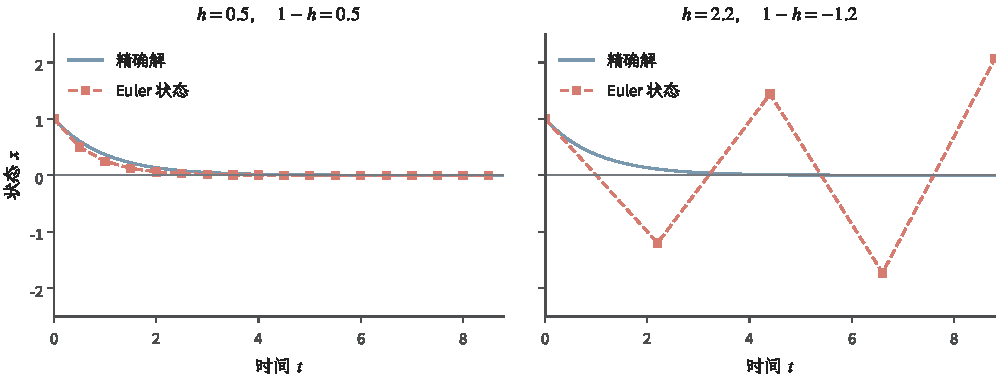
\includegraphics[width=\linewidth]{figures/math-preparation/dynamics/euler-stability.pdf}
  \caption{教学方程$\dot x=-x$、$x(0)=1$的精确解与Euler近似。蓝色实线是同一精确解，
  红色方点是各自步长下的数值状态；左图$h=0.5$衰减，右图$h=2.2$交替增长。
  两图使用相同坐标范围，连线仅显示相邻数值状态，不能解释为Euler方法在步间的精确解。}
  \label{fig:dynamical-euler-stability}
\end{figure*}

\subsection{仿射复合与前缀扫描}

轨迹的近似规则确定之后，还可改变同一递推的计算安排。前缀扫描同时求出从第一个更新起的
全部累计复合，例如$g_0$、$g_1\circ g_0$和$g_2\circ g_1\circ g_0$；它把相邻块先合并，
再逐层传播块结果，以减少串行依赖深度，数学上的时间顺序仍保持不变。考虑时变仿射递推
\begin{equation}
	\bm{x}_{k+1}= \bm{A}_{k}\bm{x}_{k}+\bm{b}_{k}. \label{eq:dynamical-affine-recurrence}
\end{equation}
把每一步表示为二元组 $g_{k}=(\bm{A}_{k},\bm{b}_{k})$，
并定义“后一步接在前一步之后”的组合
\begin{equation}
	(\bm{A}_{2},\bm{b}_{2}) \circ (\bm{A}_{1},\bm{b}_{1}) = (\bm{A}_{2}\bm{A}_{1},\,
	\bm{A}_{2}\bm{b}_{1}+\bm{b}_{2}). \label{eq:dynamical-affine-composition}
\end{equation}
直接展开三次复合可得
\[
	\begin{aligned}
	g_3\circ(g_2\circ g_1)
	&=(\bm{A}_3\bm{A}_2\bm{A}_1,\,
	\bm{A}_3\bm{A}_2\bm{b}_1+\bm{A}_3\bm{b}_2+\bm{b}_3)\\
	&=(g_3\circ g_2)\circ g_1,
	\end{aligned}
\]
所以该运算满足结合律。 由此，所有前缀 $g_{k-1}\circ\cdots\circ g_{0}$可以用并行前缀扫描组织，
再作用于$\bm{x}_{0}$得到每个状态。

结合律不等于交换律。 一般有
\[
	g_{2}\circ g_{1}\neq g_{1}\circ g_{2},
\]
因为矩阵乘法次序不同，偏置所经历的后续变换也不同。
例如令$g_1(\bm{x})=\operatorname{diag}(2,1)\bm{x}$，
$g_2(\bm{x})=\bm{x}+(1,0)^{\top}$。从$\bm{x}=\bm{0}$出发，
\[
	(g_2\circ g_1)(\bm{0})=(1,0)^{\top},\qquad
	(g_1\circ g_2)(\bm{0})=(2,0)^{\top}.
\]
同一个伸缩与平移只因交换次序就得到不同结果。
扫描算法可以改变括号位置以增加并行度， 不能改变时间顺序。
输入依赖或非线性更新若不形成封闭的结合运算，
也不能只因“看起来像递推”就使用同一扫描结构。

\section{判断扰动的长期衰减与短时放大}
\label{sec:dynamical-stability-sensitivity}

解的存在和数值计算都没有保证扰动会衰减。现在比较不同初值或输入产生的轨迹，
用谱与Lyapunov函数判断平衡点附近和较大区域内的长期行为。
原动力系统的稳定性与上节数值方法的稳定域必须分别检查，否则稳定方程也可能被步长算成发散递推。

\subsection{平衡点与稳定性}

一条轨迹最终靠近原点，不等于邻近初值在整个过程中都留在原点附近。稳定性比较的是
一组初值产生的全部正向轨迹，量词不能只落在选中的一个初值上。
\begin{definition}[平衡点与稳定性]
\label{def:dynamical-equilibrium-stability}
考虑局部Lipschitz自治系统$\dot{\bm{x}}=\bm{f}(\bm{x})$，下述稳定性均要求所涉及
初值的解对所有$t\geq0$存在。设$\bm{x}^{\star}$满足$\bm{f}(\bm{x}
^{\star})=\bm{0}$。 它称为平衡点。 平衡点在Lyapunov意义下\term{稳定}， 是指对每个$\varepsilon
>0$都存在$\delta>0$， 使$\lVert\bm{x}(0)-\bm{x}^{\star}\rVert <\delta$蕴含
\[
	\lVert\bm{x}(t)-\bm{x}^{\star}\rVert<\varepsilon \quad\text{对所有 }t\geq0.
\]
若它稳定，并且足够近的轨迹还满足 $\bm{x}(t)\to\bm{x}^{\star}$， 就称为\term{渐近稳定}。
若存在$r,C,\alpha>0$，使每个满足
$\lVert\bm{x}(0)-\bm{x}^{\star}\rVert_2<r$的初值都满足
\[
	\lVert\bm{x}(t)-\bm{x}^{\star}\rVert_2
	\leq C\mathrm{e}^{-\alpha t}
	\lVert\bm{x}(0)-\bm{x}^{\star}\rVert_2,
	\qquad t\geq0,
\]
则称该平衡点局部指数稳定。常数$C,\alpha$必须对这个邻域内的初值统一；
若同一界对任意初值成立，则称为全局指数稳定。
\end{definition}

稳定只要求轨迹不离开， 渐近稳定还要求轨迹回到平衡点。 系统$\dot{x}=0$的每个点都稳定，却没有一个孤立点吸引邻近轨迹。
稳定性也默认输入固定为所声明的值。 有外部输入时，需要另问有界输入产生多大状态响应，
不能把零输入稳定直接改写成任意输入下状态趋零。

三个稳定性概念可以在同一批标量方程上比较，见表~\ref{tab:dynamical-stability-types}。
指数条件中的统一常数决定了它比“最终回到原点”更强；不能对每个初值分别选一个
衰减率，再称为邻域上的指数稳定。

\begin{table*}[htbp]
  \centering
  \begin{tabularx}{\linewidth}{lXXX}
    \toprule
    方程与原点 & 小初值始终小 & 轨迹趋于原点 & 统一指数衰减\\
    \midrule
    $\dot x=0$ & 是，状态保持初值 & 否，非零初值不动 & 否\\
    $\dot x=-x^3$ & 是，$|x(t)|$不增 & 是，衰减为代数速度 & 否\\
    $\dot x=-x$ & 是 & 是 & 是，$|x(t)|=e^{-t}|x(0)|$\\
    \bottomrule
  \end{tabularx}
  \caption{零输入下的稳定、渐近稳定和指数稳定。第二行的解为
  $x(t)=x(0)/\sqrt{1+2x(0)^2t}$，说明吸引轨迹并不一定具有指数速度。三个例子均在
  全部$t\geq0$有解；表中比较的是相应方程原点的性质。}
  \label{tab:dynamical-stability-types}
\end{table*}

\subsection{线性系统的谱稳定判据}

对离散齐次系统
\begin{equation}
	\bm{x}_{k+1}=\bm{A}\bm{x}_{k}, \label{eq:dynamical-discrete-linear-homogeneous}
\end{equation}
有$\bm{x}_{k}=\bm{A}^{k}\bm{x}_{0}$。

\begin{theorem}[离散线性系统的渐近稳定性]
	\label{thm:dynamical-discrete-spectral-stability} 系统~\eqref{eq:dynamical-discrete-linear-homogeneous}的原点全局渐近稳定，
	当且仅当谱半径
	\[
		\rho(\bm{A}) = \max_{\lambda\in\operatorname{spec}(\bm{A})}|\lambda| <1.
	\]
\end{theorem}

\begin{proof}
	把$\bm{A}$在复数域写成Jordan形式 $\bm{A}=\bm{V}\bm{J}\bm{V}^{-1}$。 一个大小为$r$、特征值为$\lambda$的Jordan块满足
	\[
		\bm{J}_{\lambda}^{k}= \sum_{j=0}^{r-1}\binom{k}{j}\lambda^{k-j}\bm{N}^{j},
	\]
	其中$\bm{N}$为幂零矩阵。 若$|\lambda|<1$，多项式因子$k^{j}$仍被几何衰减压过，
	所以每个Jordan块趋零，进而$\bm{A}^{k}\to\bm{0}$。 这给出全局渐近稳定。

	反过来，若存在$|\lambda|>1$的特征值， 沿相应特征向量的状态会增长。 若$|\lambda|
	=1$， 沿普通特征向量的状态至少不趋零； 若相应Jordan块非平凡，还会出现多项式增长。
	因此渐近稳定要求全部特征值严格位于单位圆内。
\end{proof}

\begin{theorem}[连续线性系统的指数稳定性]
	\label{thm:dynamical-continuous-spectral-stability}
	连续线性系统$\dot{\bm{x}}=\bm{A}\bm{x}$的原点全局指数稳定，当且仅当
	$\bm{A}$的所有特征值实部严格为负。满足该条件的矩阵称为Hurwitz矩阵。
\end{theorem}

\begin{proof}
	对大小为$r$、特征值为$\lambda$的Jordan块，
	\[
		\mathrm{e}^{t(\lambda\bm{I}+\bm{N})}
		=\mathrm{e}^{\lambda t}\sum_{j=0}^{r-1}\frac{t^j}{j!}\bm{N}^j.
	\]
	若所有$\operatorname{Re}(\lambda)<0$，任选小于
	$-\max_\lambda\operatorname{Re}(\lambda)$的$\alpha>0$，
	各有限次多项式因子都可被$C\mathrm{e}^{-\alpha t}$控制。
	乘回换基矩阵后便有
	$\lVert\mathrm{e}^{t\bm{A}}\rVert\leq C\mathrm{e}^{-\alpha t}$，
	所以原点全局指数稳定。

	反过来，若某个特征值实部为正，沿对应实不变子空间存在指数增长的解；
	若实部为零，普通特征向量产生不衰减的振荡或常值解，非平凡Jordan块还会带来多项式增长。
	这些情形都不可能满足统一指数衰减界。
\end{proof}

离散系统检查单位圆，连续系统检查复平面的左半部；两者不能直接交换判据。

\subsection{Lyapunov函数与能量判据}

直接求解轨迹通常很难，但证明一个标量沿轨迹不增加可能容易得多。
\term{Lyapunov函数}（Lyapunov function）就是这样的偏离尺度；它不必等于物理能量。
\begin{definition}[Lyapunov函数]
\label{def:dynamical-lyapunov-function}
对原点为平衡点的自治系统$\dot{\bm x}=\bm f(\bm x)$，设$D$为原点的邻域。
若$V\in C^1(D)$满足$V(\bm0)=0$、$V(\bm x)>0$对所有非零$\bm x\in D$成立，
并且$\nabla V(\bm x)^\top\bm f(\bm x)\leq0$，则称$V$为该邻域内的Lyapunov函数。
若非零点处的最后一个不等式严格成立，则称它为严格Lyapunov函数。
\end{definition}
“正定”保证小能量确实表示靠近平衡点；“沿轨迹不增加”保证轨迹不能穿过更高的
能量边界。只有这两项合用，标量变化才能约束状态，而不是只约束某个可能忽略状态方向的指标。

下面的判据把这一思路落实为局部与全局稳定性条件\scite{math-khalil2002nonlinear}
\begin{theorem}[连续时间Lyapunov判据]
	\label{thm:dynamical-nonlinear-lyapunov} 设$\bm{x}^{\star}=\bm{0}$是 $\dot{\bm{x}}
=\bm{f}(\bm{x})$的平衡点，且$\bm{f}$在该点的某邻域内局部Lipschitz，使初值问题
具有唯一的最大解。若该邻域内存在连续可微函数$V$，满足
	\[
		V(\bm{0})=0,\qquad V(\bm{x})>0\quad(\bm{x}\neq\bm{0}),
	\]
	并且沿轨迹
	\[
		\dot V(\bm{x}) = \nabla V(\bm{x})^{\top}\bm{f}(\bm{x}) \leq0,
	\]
	则原点稳定。 若进一步对$\bm{x}\neq\bm{0}$有$\dot V(\bm{x})<0$，
则原点局部渐近稳定。若这些条件全局成立，$\bm{f}$在$\mathbb{R}^d$上局部Lipschitz，
且$V(\bm{x})\to\infty$随$\lVert\bm{x}\rVert\to\infty$成立，则所有最大解都可正向
延拓到任意时间，稳定性与吸引性为全局结论。
\end{theorem}

\begin{proof}
	固定一个足够小的$\varepsilon$， 使闭球包含在定理适用邻域内。 球面$\lVert\bm{x}\rVert
	=\varepsilon$是紧集， 而$V$在其上连续且正， 故最小值$c_{\varepsilon}>0$。 由$V(
	\bm{0})=0$与连续性， 可取$\delta>0$使 $\lVert\bm{x}(0)\rVert<\delta$蕴含
	$V(\bm{x}(0))<c_{\varepsilon}$。 由于$\dot V\leq0$， 轨迹不可能到达$V\geq c_{\varepsilon}$的球面，
	所以始终留在$\varepsilon$球内，得到稳定性。

	若$\dot V$负定，轨迹限制在一个紧的正子水平集$K$内。反设轨迹不趋近原点，
	则存在$\varepsilon_0>0$及趋向无穷的时刻序列，使
	$\lVert\bm{x}(t_j)\rVert\geq\varepsilon_0$。由于$\bm f$在$K$上有界，记
	$M=\sup_{\bm{x}\in K}\lVert\bm f(\bm{x})\rVert$；每次轨迹达到半径
	$\varepsilon_0$后，都至少在长度$\varepsilon_0/(2M)$的时间内留在闭环带
	$\varepsilon_0/2\leq\lVert\bm{x}\rVert\leq\sup_{\bm{z}\in K}\lVert\bm{z}\rVert$
	中。该环带紧且不含原点，连续函数$-\dot V$在其上有严格正的下界。选取互不相交
	的这些停留区间，$V$便会减少无穷大的总量，与$V\geq0$矛盾。因此轨迹趋向原点。
	径向无界性保证全局子水平集有界，轨迹无法在有限时间逃向无穷远，从而把同一论证
	扩展到任意初值。
\end{proof}

对线性系统，常取二次函数 $V(\bm{x})=\bm{x}^{\top}\bm{P}\bm{x}$。 沿$\dot{\bm{x}}=
\bm{A}\bm{x}$有
\begin{equation}
	\dot V(\bm{x}) = \bm{x}^{\top}(\bm{A}^{\top}\bm{P}+\bm{P}\bm{A}) \bm{x}. \label{eq:dynamical-continuous-lyapunov-derivative}
\end{equation}

\begin{theorem}[线性Lyapunov方程]
	\label{thm:dynamical-linear-lyapunov-equation} 矩阵$\bm{A}$为Hurwitz矩阵， 当且仅当对每个$\bm
	{Q}\succ\bm{0}$， 存在唯一$\bm{P}\succ\bm{0}$满足
	\begin{equation}
		\bm{A}^{\top}\bm{P}+\bm{P}\bm{A}= -\bm{Q}. \label{eq:dynamical-continuous-lyapunov-equation}
	\end{equation}
\end{theorem}

\begin{proof}
	若$\bm{A}$为Hurwitz矩阵，定义
	\[
		\bm{P}= \int_{0}^{\infty}\mathrm{e}^{t\bm{A}^{\top}}\bm{Q}\mathrm{e}^{t\bm{A}}
		\,\mathrm{d}t.
	\]
	指数稳定保证积分收敛。 对任意非零$\bm{x}$， 被积函数的二次型 $\lVert\bm{Q}^{1/2}
	\mathrm{e}^{t\bm{A}}\bm{x}\rVert_{2}^{2}$ 非负，并在$t=0$严格为正，所以$\bm{P}\succ
	\bm{0}$。 对被积矩阵求导并积分，
	\[
		\bm{A}^{\top}\bm{P}+\bm{P}\bm{A}= \left[ \mathrm{e}^{t\bm{A}^{\top}}\bm{Q}\mathrm{e}
		^{t\bm{A}}\right]_{0}^{\infty}= -\bm{Q}.
	\]
	唯一性可由齐次方程 $\bm{A}^{\top}\bm{D}+\bm{D}\bm{A}=\bm{0}$ 沿流积分得到$\bm{D}
	=\bm{0}$。

	反过来，若存在$\bm{P},\bm{Q}\succ\bm{0}$满足该方程， 式~\eqref{eq:dynamical-continuous-lyapunov-derivative}给出
	$\dot V=-\bm{x}^{\top}\bm{Q}\bm{x}<0$。 Lyapunov判据推出原点渐近稳定， 线性系统因而要求$\bm
	{A}$全部特征值实部为负。
\end{proof}

离散时间对应方程为
\[
	\bm{A}^{\top}\bm{P}\bm{A}-\bm{P}= -\bm{Q}.
\]
它检验一步前后能量差， 与连续时间方程的导数形式不同。

\begin{theorem}[离散时间Lyapunov方程]
	\label{thm:dynamical-discrete-lyapunov-equation}
	离散线性系统$\bm{x}_{k+1}=\bm{A}\bm{x}_k$满足$\rho(\bm{A})<1$，当且仅当对每个
	$\bm{Q}\succ\bm{0}$，存在唯一$\bm{P}\succ\bm{0}$满足
	\[
		\bm{A}^{\top}\bm{P}\bm{A}-\bm{P}=-\bm{Q}.
	\]
\end{theorem}

\begin{proof}
	若$\rho(\bm{A})<1$，定义
	\[
		\bm{P}=\sum_{j=0}^{\infty}(\bm{A}^{\top})^j\bm{Q}\bm{A}^j.
	\]
	定理~\ref{thm:dynamical-discrete-spectral-stability}及有限维范数等价性保证级数收敛。
	其首项为$\bm{Q}\succ\bm{0}$，其余项半正定，所以$\bm{P}\succ\bm{0}$。
	将级数左乘$\bm{A}^{\top}$、右乘$\bm{A}$后与原式相减，便得到Lyapunov方程。
	若$\bm{P}_1,\bm{P}_2$都是解，令$\bm{D}=\bm{P}_1-\bm{P}_2$，则
	$\bm{D}=(\bm{A}^{\top})^k\bm{D}\bm{A}^k$；令$k\to\infty$即得$\bm{D}=\bm{0}$。

	反过来，若存在$\bm{P},\bm{Q}\succ\bm{0}$满足方程，则
	\[
		V(\bm{x}_{k+1})-V(\bm{x}_k)
		=-\bm{x}_k^{\top}\bm{Q}\bm{x}_k,
		\qquad V(\bm{x})=\bm{x}^{\top}\bm{P}\bm{x}.
	\]
	由紧单位球上
	$\bm{x}^{\top}\bm{A}^{\top}\bm{P}\bm{A}\bm{x}/(\bm{x}^{\top}\bm{P}\bm{x})<1$
	取得统一上界$c<1$，故$V(\bm{x}_k)\leq c^kV(\bm{x}_0)$。
	原点指数稳定，定理~\ref{thm:dynamical-discrete-spectral-stability}于是给出$\rho(\bm{A})<1$。
\end{proof}

\subsection{LaSalle不变性与极限集}

严格负的$\dot V$迫使轨迹离开每个非平衡状态；只有$\dot V\leq0$时，轨迹却可能停留或运动在
零导数集合中。要区分这两种情况，需要描述系统长期能够留在哪些状态。
\begin{definition}[不变集合与轨迹极限集]
\label{def:dynamical-invariant-limit-sets}
设自治向量场局部Lipschitz，$\Phi_t$为其唯一解生成的流。以下集合上的解须在所有$t\geq0$存在。
集合$\Omega$称为\term{正向不变集}（positively invariant set），若从任意
$\bm{x}_0\in\Omega$出发的解在所有后续存在时刻都留在$\Omega$。
对自治系统记正向流为$\Phi_t$。集合$M$称为\term{不变集}（invariant set），若对
每个$t\geq0$都有$\Phi_t(M)=M$。等号比正向不变所要求的
$\Phi_t(M)\subseteq M$更强：它还要求$M$中的每一点都能在$M$内找到任意时长以前的
前像；等价地，每一点都位于一条始终留在$M$中的完整轨迹上。
一条正向有界轨迹$\bm{x}(t)$的\term{$\omega$极限集}定义为
\[
	\omega(\bm{x}_0)
	=\left\{\bm{z}:\ \text{存在 }t_j\to\infty
	\text{ 使 }\bm{x}(t_j)\to\bm{z}\right\}.
\]
\end{definition}
正向不变集约束从集合中每一点出发的整段未来；$\omega$极限集则记录一条轨迹在无限远时间反复接近的状态。

\begin{theorem}[LaSalle不变性原理]
	\label{thm:dynamical-lasalle-invariance}
	设自治系统$\dot{\bm{x}}=\bm{f}(\bm{x})$的向量场局部Lipschitz，
	$\Omega$是紧的正向不变集，$V$在包含$\Omega$的开邻域上连续可微，且
	$\dot V(\bm{x})=\nabla V(\bm{x})^{\top}\bm{f}(\bm{x})\leq0$。
	记$E=\{\bm{x}\in\Omega:\dot V(\bm{x})=0\}$，并令$M$为包含在$E$中的最大不变集。
	则每条从$\Omega$出发的轨迹都满足
	\[
		\operatorname{dist}(\bm{x}(t),M)\longrightarrow0.
	\]
\end{theorem}

\begin{proof}
	紧性和正向不变性使轨迹正向预紧，并排除有限时间逃逸，所以
	$\omega(\bm{x}_0)$非空且紧。函数$t\mapsto V(\bm{x}(t))$单调不增并有下界，
	因而收敛到某个$v_{\infty}$。若$\bm{z}\in\omega(\bm{x}_0)$，
	取$t_j\to\infty$使$\bm{x}(t_j)\to\bm{z}$，连续性给出$V(\bm{z})=v_{\infty}$。

	还要核对这里需要的是不变，而不只是正向不变。自治流对初值连续。对任意固定
	$s\geq0$，$\bm{x}(t_j+s)\to\Phi_s(\bm{z})$，所以
	$\Phi_s(\bm{z})\in\omega(\bm{x}_0)$，得到
	$\Phi_s(\omega(\bm{x}_0))\subseteq\omega(\bm{x}_0)$。反过来，对充分大的$j$考察
	$\bm{x}(t_j-s)$；紧性允许取子列使其收敛到某个
	$\bm{w}\in\omega(\bm{x}_0)$，而流的连续性给出
	$\Phi_s(\bm{w})=\bm{z}$。因此
	$\Phi_s(\omega(\bm{x}_0))=\omega(\bm{x}_0)$，极限集确实是不变集。

	函数$V$在$\omega(\bm{x}_0)$上恒为$v_{\infty}$。从其中任一点出发的轨迹仍留在
	该极限集，沿轨迹求导便有$\dot V=0$。于是
	$\omega(\bm{x}_0)$是$E$中的不变集，故
	$\omega(\bm{x}_0)\subseteq M$。

	还需把极限点结论转成整条尾轨迹的距离结论。若
	$\operatorname{dist}(\bm{x}(t),M)$不趋零，就存在$\varepsilon>0$和$t_j\to\infty$
	使这些距离至少为$\varepsilon$。紧性允许取收敛子列，其极限属于
	$\omega(\bm{x}_0)\subseteq M$，与距离下界矛盾。
\end{proof}

\begin{example}[阻尼振子的零导数集合]
	\label{ex:dynamical-damped-oscillator-lasalle}
	考虑
	\[
		\dot q=p,\qquad \dot p=-q-cp,\qquad c>0,
	\]
	并取$V(q,p)=(q^2+p^2)/2$。沿轨迹
	\[
		\dot V=q\dot q+p\dot p=-cp^2\leq0.
	\]
	零导数集合是整条直线$E=\{(q,p):p=0\}$，但其中$q\neq0$的点满足
	$\dot p=-q\neq0$，会立刻离开$E$。因此$E$中的最大不变子集只有原点。
	任意能量子水平集都紧且正向不变，定理~\ref{thm:dynamical-lasalle-invariance}
	遂说明所有轨迹趋向原点。仅由“$p=0$时能量瞬间不变”不能得到同一结论。
\end{example}

图~\ref{fig:reader-lasalle-zero-set}取$c=1$并从$(q,p)=(1,0)$出发。
起点虽然位于$\dot V=0$的直线上，速度$(0,-1)$却指向直线之外；随后轨迹绕原点衰减。
LaSalle需要的是能一直留在零导数集合中的完整轨迹，而不是某一瞬间导数恰为零的点。
\begin{figure}[htbp]
  \centering
  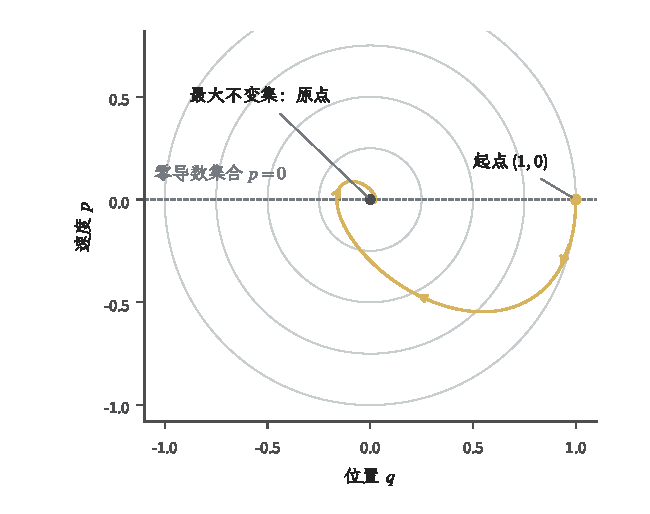
\includegraphics[width=\linewidth]{figures/math-preparation/reader-revision-dynamics/lasalle-zero-set.pdf}
  \caption{教学阻尼振子$\dot q=p$、$\dot p=-q-p$的精确轨迹，初态$(1,0)$。
  黄色轨迹在$t=0$至$12$间逐渐靠近原点，箭头表示时间前进；灰色虚线是零导数集合$p=0$，
  浅灰圆是$V=(q^2+p^2)/2$的参考等值线。整条零导数直线并不不变，原点才是其中最大不变集。}
  \label{fig:reader-lasalle-zero-set}
\end{figure}


\subsection{非正规动态与瞬态放大}

谱只决定渐近指数率，不保证每一步都缩小欧氏范数。考虑离散系统
\[
	\bm{A}=
	\begin{bmatrix}
		1/2 & K  \\
		0   & 1/2
	\end{bmatrix}, \qquad K>0.
\]
两个特征值都等于$1/2$，所以$\rho(\bm{A})<1$。然而
\[
	\bm{A}^k=
	\begin{bmatrix}
		2^{-k} & kK\,2^{-(k-1)} \\
		0      & 2^{-k}
	\end{bmatrix}.
\]
从$\bm{x}_{0}=(0,1)^{\top}$出发，第一步状态为$(K,1/2)^{\top}$；
当$K$很大时，欧氏范数立刻远大于初始范数，随后才因$k2^{-k}\to0$而衰减。

图~\ref{fig:dynamical-transient-growth}取$K=4$，与$K=0$的同谱系统比较。
非零耦合把第二个坐标中的初始扰动传入第一个坐标，造成短时放大；两者的特征值
完全相同，后期也都衰减。因而谱条件不能替代“每一步状态范数都缩小”的判断。
\begin{figure}[htbp]
  \centering
  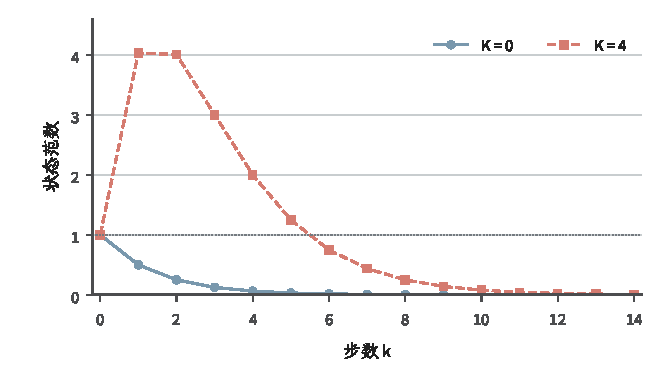
\includegraphics[width=\linewidth]{figures/math-preparation/concept-revision-dynamics/transient-growth.pdf}
  \caption{离散教学系统$\bm A=\left[\begin{smallmatrix}1/2&K\\0&1/2\end{smallmatrix}\right]$
  从$\bm x_0=(0,1)^\top$出发。蓝色圆点取$K=0$，红色方点取$K=4$；两者谱半径均为$1/2$。
  后者在前两步的欧氏范数约为$4.03$、$4.01$，然后趋零。灰线标记初始范数$1$，
  图中放大来自状态耦合，未加入输入或数值离散误差。}
  \label{fig:dynamical-transient-growth}
\end{figure}

这种现象来自矩阵非正规，即$\bm{A}^{\top}\bm{A}\neq\bm{A}\bm{A}^{\top}$。
在当前例子中，$\bm{A}=\tfrac12\bm{I}+\bm{N}$且$\bm{N}^2=\bm{0}$；
$K\neq0$时矩阵只有一个线性无关的特征向量，广义特征向量链的幂零耦合产生了
$k2^{-k}$因子。可对角化的非正规矩阵还可能通过近乎共线的特征向量，使不同衰减率的模态
先相消、后解消，从而产生另一类瞬态放大。因此，长期谱结论不能替代有限时间增益、
伪谱或合适Lyapunov范数的分析。

\subsection{初值敏感性与输入扰动响应}

若$\bm{f}$关于状态具有Lipschitz常数$L$， 两条使用同一输入的解满足
\[
	\lVert\bm{x}(t)-\widetilde{\bm{x}}(t)\rVert \leq \mathrm{e}^{L(t-t_0)}\lVert\bm
	{x}_{0}-\widetilde{\bm{x}}_{0}\rVert.
\]
这是Gronwall不等式给出的有限时间敏感性上界。 它保证连续依赖于初值， 却在$L>0$时不表示扰动衰减。

对指数稳定线性系统， 若存在$M,\alpha>0$使
$\lVert\mathrm{e}^{t\bm{A}}\rVert\leq M \mathrm{e}^{-\alpha t}$， 则式~\eqref{eq:dynamical-lti-variation-constants}给出
\[
	\lVert\bm{x}(t)\rVert \leq M\mathrm{e}^{-\alpha(t-t_0)}\lVert\bm{x}_{0}\rVert+ M
	\lVert\bm{B}\rVert \int_{t_0}^{t}\mathrm{e}^{-\alpha(t-s)}\lVert\bm{u}(s)\rVert
	\,\mathrm{d}s.
\]
有界输入因而产生有界状态， 但状态一般不会趋零。 输入、初值与模型扰动是不同来源， 稳定性结论应说明控制的是哪一种。

\section{由观测历史估计隐藏状态}
\label{sec:dynamical-stochastic-state-observation}

到这里，初值和输入给定后主要考察确定性轨迹。恢复过程噪声后，状态成为随机变量，
只能观察带噪输出时，还需区分状态分布与给定观测历史的条件分布。
本节先建立预测核和观测核，下一节才在高斯闭合条件下计算具体的滤波和平滑递推。

\subsection{用转移核与观测核表示未知状态}

恢复式~\eqref{eq:dynamical-linear-state-model}与 \eqref{eq:dynamical-linear-observation-model}中的噪声。
过程噪声$\bm{w}_{k}$直接进入状态演化， 表示模型没有显式描述的随机作用； 观测噪声$\bm
{v}_{k}$只污染读数， 不直接改变真实状态。 即使二者最终都使估计不确定，
它们在联合分布中的位置不同。

给定初始分布和输入序列， 状态转移核为
\[
	K_{k}(\bm{x},A) = \mathbb{P}\!\left( \bm{A}_{k}\bm{x}+\bm{B}_{k}\bm{u}_{k}+\bm{w}
	_{k}\in A \right).
\]
在标准加性状态空间模型中，先假设初值、各时刻过程噪声以及各时刻观测噪声相互独立，
输入序列为给定量。于是$\bm{w}_k$在给定$\bm{x}_k$后，与
$\sigma(\bm{x}_{0:k-1},\bm{y}_{1:k},\bm{u}_{0:k})$条件独立，状态过程满足
条件Markov性质
\[
	\mathbb{P}( \bm{x}_{k+1}\in A \mid \bm{x}_{0:k},\bm{y}_{1:k},\bm{u}_{0:k}) = K_{k}
	(\bm{x}_{k},A).
\]
Markov性质针对真实状态。 观测序列自身通常不是Markov链， 因为当前观测未必包含预测下一观测所需的全部状态信息。

与状态转移核相对，观测核
\[
	G_k(\bm{x},B)
	=\mathbb{P}(\bm{y}_k\in B\mid \bm{x}_k=\bm{x})
\]
规定给定当前状态后会看到什么。在标准状态空间模型中，给定$\bm{x}_k$以后，
$\bm{y}_k$与更早的状态、观测和噪声条件独立。若过程噪声与观测噪声相关，
或者传感器还直接依赖旧状态，就必须把相关变量并入联合状态或显式修改这个条件独立结构。

记$\mathcal{Y}_{k}=\sigma(\bm{y}_{1},\ldots,\bm{y}_{k})$。在只观察$\bm{y}$时，
可用于预测未来的对象变成状态的条件分布。
\begin{definition}[滤波分布]
\label{def:dynamical-filtering-distribution}
对标准状态空间模型中的欧氏状态和观测，给定$\mathcal Y_k$后的状态条件概率核
\begin{equation}
	\pi_{k}(A) = \mathbb{P}(\bm{x}_{k}\in A\mid\mathcal{Y}_{k}), \label{eq:dynamical-filtering-distribution}
\end{equation}
称为\term{滤波分布}（filtering distribution），其中$A$遍历状态空间的Borel集合。
\end{definition}
它是根据截至当前的观测对隐藏状态形成的条件分布。
真实状态$\bm{x}_{k}$、带噪读数$\bm{y}_{k}$与条件分布$\pi_{k}$
分别是潜在对象、数据和推断结果，不能用同一个“状态”含混指代。

信息不足即使没有观测噪声也可能出现。例如$\bm{x}_k=(x_{1,k},x_{2,k})^{\top}$，
而传感器只返回$y_k=x_{1,k}+x_{2,k}$。观测$y_k=1$不能区分
$(1,0)^{\top}$与$(0,1)^{\top}$；动力学和后续观测或许能逐步区分这两个方向，
但这需要额外结构。第~\ref{chap:control-theory}章将用可观测性和可检测性精确刻画线性系统中哪些方向可以恢复。

\subsection{先传播预测，再用新证据校正}

设当前滤波分布为$\pi_{k-1}$。 先通过状态转移核得到预测分布
\begin{equation}
	\pi_{k\mid k-1}(A) = \int K_{k-1}(\bm{x},A) \,\pi_{k-1}(\mathrm{d}\bm{x}). \label{eq:dynamical-general-prediction-kernel}
\end{equation}
要把校正写成密度形式，还需假设存在与状态$\bm{x}$无关的共同$\sigma$有限支配测度
$\nu_k$以及联合可测函数$g_k$，使
\[
	G_k(\bm{x},\mathrm{d}\bm{y})
	=g_k(\bm{y}\mid\bm{x})\nu_k(\mathrm{d}\bm{y}).
\]
观测$\bm{y}_{k}$到来后，再用似然密度
$g_{k}(\bm{y}_{k}\mid\bm{x}_{k})$重新加权：
\begin{equation}
	\pi_{k}(\mathrm{d}\bm{x}) =
	\frac{g_{k}(\bm{y}_{k}\mid\bm{x})\pi_{k\mid k-1}(\mathrm{d}\bm{x})}
	{\int g_{k}(\bm{y}_{k}\mid\bm{z})\pi_{k\mid k-1}(\mathrm{d}\bm{z})}. \label{eq:dynamical-general-bayes-filter}
\end{equation}
这个公式适用于分母有限且严格为正的观测值。预测传播动力学不确定性，
校正利用新观测改变相对权重；两步分别来自全概率公式和Bayes公式。

\begin{example}[两状态模型的一次预测与校正]
	\label{ex:dynamical-two-state-bayes-filter}
	设隐藏状态取值于$\{0,1\}$，当前滤波概率为
	$\pi_0(0)=0.7$、$\pi_0(1)=0.3$，转移矩阵按“当前状态为行、下一状态为列”写成
	\[
		\bm{P}=
		\begin{bmatrix}
			0.8 & 0.2\\
			0.1 & 0.9
		\end{bmatrix}.
	\]
	一步预测得到
	\[
		\pi_{1\mid0}(1)=0.7\times0.2+0.3\times0.9=0.41,\qquad
		\pi_{1\mid0}(0)=0.59.
	\]
	再设观测$y_1\in\{0,1\}$满足
	$\mathbb{P}(y_1=1\mid x_1=0)=0.2$、
	$\mathbb{P}(y_1=1\mid x_1=1)=0.8$。实际看到$y_1=1$后，
	\[
		\pi_1(1)
		=\frac{0.8\times0.41}{0.2\times0.59+0.8\times0.41}
		=\frac{164}{223}\approx0.735.
	\]
	预测步骤把上一时刻的不确定性穿过转移矩阵，校正步骤才用观测似然重新分配概率。
	整个计算只保存$\pi_0$而不保存更早观测，正是因为标准条件独立结构已经把过去信息压缩进当前滤波分布。
\end{example}

\begin{example}[带泄漏温度的间接观测]
	\label{ex:dynamical-noisy-temperature} 设房间相对环境的温差满足
	\[
		x_{k+1}=0.9x_{k}+u_{k}+w_{k}, \qquad y_{k}=x_{k}+v_{k}.
	\]
	即使$v_{k}=0$，未来温差仍因$w_{k}$不确定； 即使$w_{k}=0$，当前温差仍不能从带噪$y
	_{k}$精确知道。 若两种噪声同时存在， 预测阶段因过程噪声扩大不确定性， 校正阶段再根据传感器精度缩小不确定性。
	把$y_{k}$直接当作$x_{k}$会忽略观测噪声， 只按确定递推外推又会忽略过程噪声。
\end{example}

\subsection{在线性高斯模型中封闭分布递推}
\label{sec:dynamical-kalman-rts}

为了得到解析递推，下面采用有限时域线性高斯模型：
\begin{align*}
	\bm{x}_{0} & \sim \mathcal{N}(\bm{m}_{0\mid0},\bm{P}_{0\mid0}), \\
	\bm{w}_{k} & \sim \mathcal{N}(\bm{0},\bm{\Sigma}_{\mathrm{w},k}),               \\
	\bm{v}_{k} & \sim \mathcal{N}(\bm{0},\bm{\Sigma}_{\mathrm{v},k}).
\end{align*}
假设初值、全部过程噪声和全部观测噪声彼此独立，输入与系统矩阵为给定量。允许
$\bm{\Sigma}_{\mathrm{w},k}$半正定，并先假设
$\bm{\Sigma}_{\mathrm{v},k}\succ\bm{0}$，以保证后续创新协方差可逆。

线性变换保持高斯性， 联合高斯的条件分布仍为高斯。 因此只需递推条件均值与条件协方差，
便能完整表示每个滤波分布。 若初值或噪声非高斯， 均值和协方差更新仍可能给出最佳线性估计，
却不再完整描述条件分布，也不能无条件称为精确Bayes滤波。

高斯性使整个分布可以由均值与协方差保存，但递推以前仍须先固定允许使用哪一段观测。

\subsubsection{预测、滤波与平滑的信息条件}

记
\begin{align*}
	\bm{m}_{k\mid j} & := \mathbb{E}[\bm{x}_{k}\mid\mathcal{Y}_{j}],         \\
	\bm{P}_{k\mid j} & := \operatorname{Cov}(\bm{x}_{k}\mid\mathcal{Y}_{j}).
\end{align*}
一步预测使用$\mathcal{Y}_{k-1}$估计$\bm{x}_{k}$， 滤波使用$\mathcal{Y}_{k}$估计同一当前状态，
平滑则在固定终点$T>k$后使用$\mathcal{Y}_{T}$重新估计过去状态。
未来观测能够帮助平滑， 因为它们包含过去状态经过动力学传播后的信息。

表~\ref{tab:dynamical-estimation-information}固定同一个目标$x_k$，只改变允许使用的
观测。区别在信息集合，而不在是否使用某一种算法。在线决策到时刻$k$只能调用前两行；
把事后平滑结果当作在线估计，会让当前决策使用尚未发生的观测。

\begin{table}[htbp]
  \centering
  \begin{tabularx}{\linewidth}{lXX}
    \toprule
    推断 & 条件分布 & 可用观测\\
    \midrule
    一步预测 & $P(\bm{x}_k\mid\mathcal Y_{k-1})$ & 新读数到来之前的历史\\
    当前滤波 & $P(\bm{x}_k\mid\mathcal Y_k)$ & 截至当前的新旧读数\\
    固定区间平滑 & $P(\bm{x}_k\mid\mathcal Y_T)$，$T>k$ & 事后取得的未来读数\\
    \bottomrule
  \end{tabularx}
  \caption{预测、滤波与平滑针对同一状态，却允许使用不同信息。向量状态的条件分布采用
  同样的口径，$\mathcal Y_j$表示截至时刻$j$的观测所生成的信息。}
  \label{tab:dynamical-estimation-information}
\end{table}

\subsubsection{预测均值与协方差传播}

假设
\[
	\bm{x}_{k-1}\mid\mathcal{Y}_{k-1}\sim \mathcal{N}( \bm{m}_{k-1\mid k-1}, \bm{P}
	_{k-1\mid k-1}).
\]
由状态方程和独立零均值过程噪声，
\begin{align}
	\bm{m}_{k\mid k-1} & = \bm{A}_{k-1}\bm{m}_{k-1\mid k-1}+\bm{B}_{k-1}\bm{u}_{k-1}, \label{eq:dynamical-kalman-predicted-mean}              \\
	\bm{P}_{k\mid k-1} & = \bm{A}_{k-1}\bm{P}_{k-1\mid k-1}\bm{A}_{k-1}^{\top}+\bm{\Sigma}_{\mathrm{w},k-1}. \label{eq:dynamical-kalman-predicted-covariance}
\end{align}
交叉协方差项消失的依据是 $\bm{w}_{k-1}$与 $\bm{x}_{k-1}\mid\mathcal{Y}_{k-1}$独立且均值为零。
若过程噪声与旧状态相关， 式~\eqref{eq:dynamical-kalman-predicted-covariance} 还要保留相应交叉项。

\subsubsection{条件高斯更新与Kalman滤波}

给定$\mathcal{Y}_{k-1}$， 预测状态与新观测的联合分布为
\begin{equation}
	\begin{bmatrix}
		\bm{x}_{k} \\
		\bm{y}_{k}
	\end{bmatrix}
	\Biggm|\mathcal{Y}_{k-1}\sim \mathcal{N}\left(
	\begin{bmatrix}
		\bm{m}_{k\mid k-1}           \\
		\bm{C}_{k}\bm{m}_{k\mid k-1}
	\end{bmatrix},
	\begin{bmatrix}
		\bm{P}_{k\mid k-1}           & \bm{P}_{k\mid k-1}\bm{C}_{k}^{\top} \\
		\bm{C}_{k}\bm{P}_{k\mid k-1} & \bm{S}_{k}
	\end{bmatrix}
	\right), \label{eq:dynamical-kalman-joint-gaussian}
\end{equation}
其中
\begin{equation}
	\bm{S}_{k}= \bm{C}_{k}\bm{P}_{k\mid k-1}\bm{C}_{k}^{\top}+\bm{\Sigma}_{\mathrm{v},k}\label{eq:dynamical-kalman-innovation-covariance}
\end{equation}
是\term{创新协方差}，
\[
	\bm{r}_{k}= \bm{y}_{k}-\bm{C}_{k}\bm{m}_{k\mid k-1}
\]
是创新，即新观测超出预测观测的部分。

由于$\bm{\Sigma}_{\mathrm{v},k}\succ\bm{0}$， 有$\bm{S}_{k}\succ\bm{0}$并可逆。 把第~\ref{sec:probability-random-vectors-transformations}节的
条件高斯公式用于联合分布~\eqref{eq:dynamical-kalman-joint-gaussian}， 得到
\begin{align}
	\bm{K}_{k}       & = \bm{P}_{k\mid k-1}\bm{C}_{k}^{\top}\bm{S}_{k}^{-1}, \label{eq:dynamical-kalman-gain}                       \\
	\bm{m}_{k\mid k} & = \bm{m}_{k\mid k-1}+\bm{K}_{k}\bm{r}_{k}, \label{eq:dynamical-kalman-filtered-mean}                         \\
	\bm{P}_{k\mid k} & = \bm{P}_{k\mid k-1}- \bm{K}_{k}\bm{S}_{k}\bm{K}_{k}^{\top}. \label{eq:dynamical-kalman-filtered-covariance}
\end{align}
式~\eqref{eq:dynamical-kalman-gain}中的 $\bm{K}_{k}$称为Kalman增益。 它不是手工设定的学习率，
而是预测误差与观测误差协方差共同决定的条件高斯系数
\scite{math-kalman1960filtering}

\begin{theorem}[有限时域Kalman滤波]
	\label{thm:dynamical-finite-horizon-kalman-filter} 在本节线性高斯初值、独立高斯噪声及
	$\bm{S}_{k}$可逆的条件下， 递推~\eqref{eq:dynamical-kalman-predicted-mean}至
	\eqref{eq:dynamical-kalman-filtered-covariance} 精确给出
	\[
		\bm{x}_{k}\mid\mathcal{Y}_{k}\sim \mathcal{N}( \bm{m}_{k\mid k}, \bm{P}_{k\mid
		k})
	\]
	对每个有限$k$成立。
\end{theorem}

\begin{proof}
	对$k$归纳。 初值按假设为高斯。 若$\bm{x}_{k-1}\mid\mathcal{Y}_{k-1}$为高斯，
	线性状态方程与独立高斯过程噪声使 $\bm{x}_{k}\mid\mathcal{Y}_{k-1}$仍为高斯，
	其均值和协方差由 \eqref{eq:dynamical-kalman-predicted-mean}与 \eqref{eq:dynamical-kalman-predicted-covariance}给出。
	观测又是预测状态与独立高斯噪声的线性组合， 所以联合分布为 \eqref{eq:dynamical-kalman-joint-gaussian}。
	条件高斯公式给出 \eqref{eq:dynamical-kalman-filtered-mean}与 \eqref{eq:dynamical-kalman-filtered-covariance}，
	完成归纳。
\end{proof}

协方差更新还可写成Joseph形式
\begin{equation}
	\bm{P}_{k\mid k}= (\bm{I}-\bm{K}_{k}\bm{C}_{k}) \bm{P}_{k\mid k-1}(\bm{I}-\bm{K}
	_{k}\bm{C}_{k})^{\top}+ \bm{K}_{k}\bm{\Sigma}_{\mathrm{v},k}\bm{K}_{k}^{\top}. \label{eq:dynamical-kalman-joseph-form}
\end{equation}
代入Kalman增益并展开，可化为 式~\eqref{eq:dynamical-kalman-filtered-covariance}。
Joseph形式把两类误差来源都写成半正定项，
在有限精度实现中更容易维持协方差的对称与半正定。 实现时也应通过线性求解获得
$\bm{S}_{k}^{-1}\bm{r}_{k}$， 而不是显式形成逆矩阵。

\begin{example}[标量观测怎样权衡预测与读数]
	\label{ex:dynamical-scalar-kalman-update} 若预测方差为$p^{-}$，观测为$y=x+v$， 且$v
	\sim\mathcal{N}(0,r)$，则
	\[
		K=\frac{p^{-}}{p^{-}+r}, \qquad m^{+}=m^{-}+K(y-m^{-}), \qquad
		p^{+}=\frac{p^{-}r}{p^{-}+r}.
	\]
	当$r$很小，增益接近$1$，更新更相信读数； 当$r$很大，增益接近$0$，更新更相信预测。
	即使$r\to0$， 只有被直接观测的方向会被精确校正； 多维系统中未被$\bm{C}_{k}$区分的方向仍可能保留不确定性。

	例如$m^-=0$、$p^-=4$、$r=1$且实际读数$y=2$时，
	\[
		K=\frac45,\qquad m^+=\frac85,\qquad p^+=\frac45.
	\]
	后验均值位于预测均值$0$与读数$2$之间，后验方差也小于预测方差和观测噪声方差；
	后一比较依赖两项误差独立且方差均为正。
\end{example}

图~\ref{fig:dynamical-kalman-density-update}展示刚才的标量计算。后验向读数移动，同时
变窄，因为独立的新读数排除了部分原本可能的状态。密度曲线的纵轴是密度而非单点概率，
曲线变高表示质量集中，曲线下的总面积仍为$1$。这个几何解释只适用于此处的高斯、
独立噪声设定；观测值与预测不一致，并不总意味着真实过程本身发生了跳变。

\begin{figure}[htbp]
  \centering
  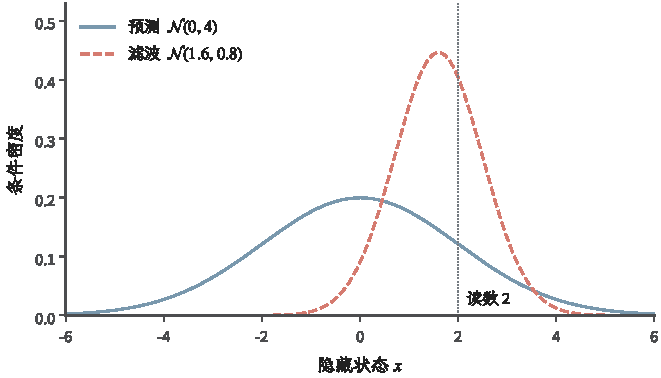
\includegraphics[width=\linewidth]{figures/math-preparation/dynamics/kalman-density-update.pdf}
  \caption{标量Kalman更新的教学例。蓝色曲线为预测$\mathcal N(0,4)$，红色曲线为观察
  $y=2$后得到的$\mathcal N(1.6,0.8)$，观测噪声方差为$1$，虚线标记实际读数。
  这里$\mathcal N$的第二个参数是方差；比较的是同一隐藏状态在新观测前后的条件密度。}
  \label{fig:dynamical-kalman-density-update}
\end{figure}

\subsection{利用未来观测修正过去状态}

滤波只向前传递。 固定终点$T$后， Rauch--Tung--Striebel（RTS）平滑器从 $k=T-1$向后计算
$p(\bm{x}_{k}\mid\mathcal{Y}_{T})$\scite{math-rauch1965smoothing} 关键是先求
$p(\bm{x}_{k}\mid\bm{x}_{k+1},\mathcal{Y}_{k})$。

给定$\mathcal{Y}_{k}$， 由状态方程可得联合高斯
\[
	\begin{bmatrix}
		\bm{x}_{k}   \\
		\bm{x}_{k+1}
	\end{bmatrix}
	\Biggm|\mathcal{Y}_{k}\sim \mathcal{N}\left(
	\begin{bmatrix}
		\bm{m}_{k\mid k}   \\
		\bm{m}_{k+1\mid k}
	\end{bmatrix},
	\begin{bmatrix}
		\bm{P}_{k\mid k}           & \bm{P}_{k\mid k}\bm{A}_{k}^{\top} \\
		\bm{A}_{k}\bm{P}_{k\mid k} & \bm{P}_{k+1\mid k}
	\end{bmatrix}
	\right).
\]
若$\bm{P}_{k+1\mid k}$可逆， 条件高斯公式给出
\begin{align}
	\bm{J}_{k}                                                       & = \bm{P}_{k\mid k}\bm{A}_{k}^{\top}\bm{P}_{k+1\mid k}^{-1}, \label{eq:dynamical-rts-gain}                                   \\
	\mathbb{E}[ \bm{x}_{k}\mid \bm{x}_{k+1},\mathcal{Y}_{k}]         & = \bm{m}_{k\mid k}+ \bm{J}_{k}(\bm{x}_{k+1}-\bm{m}_{k+1\mid k}), \label{eq:dynamical-rts-one-step-conditional-mean}         \\
	\operatorname{Cov}( \bm{x}_{k}\mid \bm{x}_{k+1},\mathcal{Y}_{k}) & = \bm{P}_{k\mid k}- \bm{J}_{k}\bm{P}_{k+1\mid k}\bm{J}_{k}^{\top}. \label{eq:dynamical-rts-one-step-conditional-covariance}
\end{align}

\begin{theorem}[有限时域RTS平滑]
	\label{thm:dynamical-rts-smoother} 在有限时域Kalman滤波条件下， 并假设每个$\bm{P}
	_{k+1\mid k}$可逆， 以
	\[
		\bm{m}_{T\mid T},\qquad \bm{P}_{T\mid T}
	\]
	为终点，向后递推
	\begin{align}
		\bm{m}_{k\mid T} & = \bm{m}_{k\mid k}+ \bm{J}_{k}(\bm{m}_{k+1\mid T}-\bm{m}_{k+1\mid k}), \label{eq:dynamical-rts-smoothed-mean}                       \\
		\bm{P}_{k\mid T} & = \bm{P}_{k\mid k}+ \bm{J}_{k}(\bm{P}_{k+1\mid T}-\bm{P}_{k+1\mid k}) \bm{J}_{k}^{\top}\label{eq:dynamical-rts-smoothed-covariance}
	\end{align}
	可精确得到 $\bm{x}_{k}\mid\mathcal{Y}_{T}$的均值与协方差。
\end{theorem}

\begin{proof}
	状态的Markov结构与观测条件独立性给出
	\[
		p(\bm{x}_{k}\mid\bm{x}_{k+1},\mathcal{Y}_{T}) = p(\bm{x}_{k}\mid\bm{x}_{k+1},
		\mathcal{Y}_{k}).
	\]
	未来观测$\bm{y}_{k+1:T}$在给定$\bm{x}_{k+1}$后， 不再提供关于$\bm{x}_{k}$的额外信息。
	因此
	\begin{equation}
		p(\bm{x}_{k}\mid\mathcal{Y}_{T}) = \int p(\bm{x}_{k}\mid\bm{x}_{k+1},\mathcal{Y}
		_{k}) p(\bm{x}_{k+1}\mid\mathcal{Y}_{T}) \,\mathrm{d}\bm{x}_{k+1}. \label{eq:dynamical-rts-backward-factorization}
	\end{equation}

	对式~\eqref{eq:dynamical-rts-one-step-conditional-mean} 关于 $\bm{x}_{k+1}\mid\mathcal{Y}
	_{T}$ 取期望，塔式性质立即给出 \eqref{eq:dynamical-rts-smoothed-mean}。

	再使用全协方差公式。 式~\eqref{eq:dynamical-rts-one-step-conditional-covariance}
	不依赖$\bm{x}_{k+1}$， 构成条件内协方差项。 条件均值关于$\bm{x}_{k+1}$的随机部分为
	$\bm{J}_{k}\bm{x}_{k+1}$， 其协方差为
	$\bm{J}_{k}\bm{P}_{k+1\mid T}\bm{J}_{k}^{\top}$。 两项相加得到
	\[
		\bm{P}_{k\mid T}= \bm{P}_{k\mid k}- \bm{J}_{k}\bm{P}_{k+1\mid k}\bm{J}_{k}^{\top}
		+ \bm{J}_{k}\bm{P}_{k+1\mid T}\bm{J}_{k}^{\top},
	\]
	整理即为 \eqref{eq:dynamical-rts-smoothed-covariance}。 从$T$向后归纳便完成证明。
\end{proof}

\begin{example}[未来观测降低过去状态的不确定性]
	\label{ex:dynamical-scalar-rts-update}
	取标量模型$x_1=x_0+w_0$、$y_1=x_1+v_1$，并设
	$m_{0\mid0}=0$、$P_{0\mid0}=1$、
	$\bm{\Sigma}_{\mathrm{w},0}=1$、$\bm{\Sigma}_{\mathrm{v},1}=2/3$。
	若观察到$y_1=2$，前向预测与滤波给出
	\[
		m_{1\mid0}=0,\quad P_{1\mid0}=2,\qquad
		m_{1\mid1}=\frac32,\quad P_{1\mid1}=\frac12.
	\]
	RTS增益为$J_0=P_{0\mid0}/P_{1\mid0}=1/2$，所以
	\[
		m_{0\mid1}=\frac34,\qquad
		P_{0\mid1}=1+\frac14\left(\frac12-2\right)=\frac58.
	\]
	时刻$0$没有新观测，滤波估计仍为均值$0$、方差$1$；看到时刻$1$的读数后，
	平滑估计把过去均值移向与该读数一致的方向，并把方差从$1$降到$5/8$。
	这说明未来证据改变的是过去状态的条件分布，而不是物理上回到过去改变状态。
\end{example}

若协方差奇异， 可以在高斯分布的支持子空间上使用广义逆， 但必须同时检查观测值是否位于相应支持内。
直接把普通逆替换成伪逆而不处理支持条件， 可能写出形式正确却没有对应条件分布的公式。

\subsection{区分边缘估计、路径最优与近似后验}

在线性高斯模型下，$\bm{m}_{k\mid T}$是平方损失下估计$\bm{x}_{k}$的条件均值。
当边缘后验协方差正定时，它也是相对于Lebesgue密度的边缘众数；
整条路径的后验协方差正定时，联合众数也等于联合均值，所以各时刻分量与平滑均值一致。
退化高斯分布没有相对于全维Lebesgue测度的密度；若改用其仿射支持上的密度，
均值仍可视为该意义下的众数。在非高斯模型中，
每个时刻的边缘众数拼接起来不一定构成联合后验的最大概率路径。
Viterbi式路径最优与逐时刻边缘最优回答不同问题。

非线性状态模型
\[
	\bm{x}_{k+1}=\bm{f}_{k}(\bm{x}_{k})+\bm{w}_{k}, \qquad \bm{y}_{k}=\bm{g}_{k}(\bm
	{x}_{k})+\bm{v}_{k}
\]
一般不保持高斯闭合。 扩展Kalman滤波在当前均值附近用Jacobian矩阵线性化， 近似的是局部函数。
无迹Kalman滤波选取一组确定性sigma点传播， 再匹配变换后均值与协方差， 近似的是矩传播。
二者都不会把一般非高斯后验变成精确高斯。 多峰、强非线性或硬约束下， 粒子方法、混合表示或问题专用推断可能更合适。

本节只给出有限时域递推。 滤波增益是否收敛、极限协方差是否唯一稳定，
还需要系统的可检测性、噪声作用范围等条件，
这些条件将在第~\ref{chap:control-theory}章结合系统结构讨论。 该章沿用本章的
$\bm{x}_{k}$、$\bm{u}_{k}$、$\bm{y}_{k}$作为状态、输入和输出，只把时间下标改为$t$；
本章给定$\bm{u}_{k}$并令$\bm{y}_{k}=\bm{C}_{k}\bm{x}_{k}+\bm{v}_{k}$，
该章则把$\bm{u}_{t}$改为反馈选择，并允许$\bm{D}\bm{u}_{t}$直接进入输出。

\section{由平均漂移判断随机参数更新的稳定方向}
\label{sec:dynamical-mean-dynamics-linear-recursion}

状态估计根据观测更新未知状态的分布；随机逼近则根据观测更新待求解的参数。
本节转向后一个对象，复用第~\ref{chap:stochastic-processes-and-approximation}章的
平均ODE方法，用矩阵结构检查平均漂移的稳定方向。平均方程稳定仍不足以保证随机递推收敛，
噪声、步长、访问制度和迭代有界性需要一并满足。

\subsection{线性平均漂移与稳定方向}

第~\ref{sec:stoch-approximation-markov-noise}节把随机逼近写成
\[
	\bm{\theta}^{(k+1)}= \bm{\theta}^{(k)}+ \alpha_{k}[ \overline{\bm{h}}(\bm{\theta}
	^{(k)}) +\bm{\xi}_{k+1}+\bm{r}_{k+1}].
\]
对线性平均漂移，常见形式为
\begin{equation}
	\overline{\bm{h}}(\bm{\theta}) = \bm{b}-\bm{A}\bm{\theta}. \label{eq:dynamical-linear-mean-drift}
\end{equation}
若$\bm{A}$可逆，候选平衡点为 $\bm{\theta}^{\star}=\bm{A}^{-1}\bm{b}$。 令$\bm{e}=
\bm{\theta}-\bm{\theta}^{\star}$， 平均ODE变成
\begin{equation}
	\dot{\bm{e}}=-\bm{A}\bm{e}. \label{eq:dynamical-linear-mean-error-ode}
\end{equation}
稳定性检查的是$-\bm{A}$是否Hurwitz， 等价于$\bm{A}$的全部特征值实部为正。 漏掉负号会把稳定与发散方向完全颠倒。

若$\bm{A}$对称正定， $V(\bm{e})=\lVert\bm{e}\rVert_{2}^{2}/2$满足
\[
	\dot V = -\bm{e}^{\top}\bm{A}\bm{e}<0.
\]
但随机逼近中的$\bm{A}$常常不对称， 也未必是某个标量目标的Hessian矩阵。 此时不能因为更新看起来像“下降”就套用凸优化曲率。

\subsection{对称部分的充分稳定条件}

对一般实矩阵，
\[
	\bm{e}^{\top}\bm{A}\bm{e}= \bm{e}^{\top}\frac{\bm{A}+\bm{A}^{\top}}{2}\bm{e},
\]
因为反对称部分的二次型为零。 所以若
\begin{equation}
	\frac{\bm{A}+\bm{A}^{\top}}{2}\succ\bm{0}, \label{eq:dynamical-positive-symmetric-part}
\end{equation}
欧氏能量严格下降， 从而平均ODE稳定。 这是方便的充分条件。

它不是必要条件。 例如
\[
	\bm{A}=
	\begin{bmatrix}
		1 & 10 \\
		0 & 1
	\end{bmatrix}
\]
的特征值实部均为正， 所以$-\bm{A}$稳定； 但其对称部分
\[
	\frac{\bm{A}+\bm{A}^{\top}}{2}=
	\begin{bmatrix}
		1 & 5 \\
		5 & 1
	\end{bmatrix}
\]
有一个负特征值。 欧氏范数可能暂时增长，
仍存在另一个二次Lyapunov函数证明长期稳定。

由定理~\ref{thm:dynamical-linear-lyapunov-equation}， 只要$-\bm{A}$为Hurwitz矩阵，
对任意$\bm{Q}\succ\bm{0}$都存在$\bm{P}\succ\bm{0}$满足
\begin{equation}
	\bm{A}^{\top}\bm{P}+\bm{P}\bm{A}= \bm{Q}. \label{eq:dynamical-mean-drift-lyapunov}
\end{equation}
于是 $V(\bm{e})=\bm{e}^{\top}\bm{P}\bm{e}$ 沿式~\eqref{eq:dynamical-linear-mean-error-ode}满足
$\dot V=-\bm{e}^{\top}\bm{Q}\bm{e}$。 矩阵$\bm{P}$选择了适合非对称漂移的加权几何。

\subsection{平稳Markov算子与加权漂移}

线性时序差分学习提供了一个重要例子。固定策略诱导有限状态Markov转移矩阵$\bm{P}_{\pi}$，
设其平稳分布为$\bm{d}$， 并令$\bm{D}=\operatorname{diag}(\bm{d})$。 特征矩阵为$\bm
{\Phi}\in\mathbb{R}^{n\times q}$， 折扣因子满足$0\leq\gamma<1$。 同策略线性TD的平均漂移可写成
\begin{equation}
\overline{\bm{h}}(\bm{\theta}) = \bm{b}-\bm{A}_{\mathrm{TD}}\bm{\theta},
\qquad
\bm{A}_{\mathrm{TD}}= \bm{\Phi}^{\top}\bm{D}
(\bm{I}-\gamma\bm{P}_{\pi}) \bm{\Phi}.
\label{eq:dynamical-td-mean-matrix}
\end{equation}

若某些$d_i=0$，$\lVert\bm{z}\rVert_{\bm D}
=(\bm z^\top\bm D\bm z)^{1/2}$只是在全空间上的半范数。为使用通常的范数与
Cauchy--Schwarz表述，下文先假设所考虑的状态满足$d_i>0$；更一般地，
后续严格稳定结论只需直接假设
$\bm\Phi^\top\bm D\bm\Phi\succ\bm0$。
平稳性使$\bm{P}_{\pi}$在$\bm{D}$加权二范数下非扩张。对任意向量$\bm{z}$，
Jensen不等式给出
\[
	(\bm{P}_{\pi}\bm{z})_{i}^{2}
	\leq \sum_{j}(\bm{P}_{\pi})_{i,j}z_{j}^{2}.
\]
乘以$d_{i}$并求和，再用
$\sum_{i}d_{i}(\bm{P}_{\pi})_{i,j}=d_{j}$，得到
\begin{equation}
	\lVert\bm{P}_{\pi}\bm{z}\rVert_{\bm{D}}\leq \lVert\bm{z}\rVert_{\bm{D}}. \label{eq:dynamical-markov-contraction-weighted}
\end{equation}
因此由Cauchy--Schwarz不等式，
\[
	\langle\bm{z},\bm{P}_{\pi}\bm{z}\rangle_{\bm{D}}
	\leq \lVert\bm{z}\rVert_{\bm{D}}\lVert
	\bm{P}_{\pi}\bm{z}\rVert_{\bm{D}}
	\leq \lVert\bm{z}\rVert_{\bm{D}}^{2}.
\]
令$\bm{z}=\bm{\Phi}\bm{c}$，可得
\begin{align}
	\bm{c}^{\top}\bm{A}_{\mathrm{TD}}\bm{c}
	& = \lVert\bm{\Phi}\bm{c}\rVert_{\bm{D}}^{2}
	- \gamma \langle \bm{\Phi}\bm{c},
	\bm{P}_{\pi}\bm{\Phi}\bm{c}\rangle_{\bm{D}}\notag \\
	                          & \geq (1-\gamma) \lVert\bm{\Phi}\bm{c}\rVert_{\bm{D}}^{2}. \label{eq:dynamical-td-positive-drift}
\end{align}
若特征协方差 $\bm{\Phi}^{\top}\bm{D}\bm{\Phi}\succ\bm{0}$， 则右侧对$\bm{c}\neq\bm
{0}$严格为正。因此$\bm{A}_{\mathrm{TD}}$的对称部分正定，平均ODE具有唯一全局指数稳定平衡。

这个证明使用了固定策略下的平稳权重、$\gamma<1$和加权特征协方差正定。
在所有$d_i>0$的假设下，最后一个条件等价于$\bm\Phi$满列秩；若允许零平稳质量，
普通满列秩并不足够。离策略采样把$\bm{D}$换成另一访问分布，
而转移算子仍来自目标策略， 式~\eqref{eq:dynamical-markov-contraction-weighted}
可能不再成立。 所以同策略稳定不能直接推出离策略稳定。

\subsection{平均ODE与随机递推的收敛条件}

平均ODE只描述噪声抵消后的方向。 要把稳定平衡转成
$\bm{\theta}^{(k)}\to\bm{\theta}^{\star}$， 仍需核对第~\ref{sec:stoch-approximation-markov-noise}节的条件：
\[
	\sum_{k}\alpha_{k}=\infty, \qquad \sum_{k}\alpha_{k}^{2}<\infty,
\]
加权噪声在有限算法时间窗内消失， 偏差项可控，并且迭代几乎必然有界。
Markov采样还需要Poisson方程或相应混合条件， 不能只用平稳平均替代相关噪声分析。

标量线性递推可以直接显示这些条件怎样配合。设
\[
	\theta^{(k+1)}
	=\theta^{(k)}+\alpha_k\bigl[b-a\theta^{(k)}+\xi_{k+1}\bigr],
	\qquad a>0,
\]
其中$\mathbb{E}[\xi_{k+1}\mid\mathcal{F}_k]=0$且
$\mathbb{E}[\xi_{k+1}^2\mid\mathcal{F}_k]\leq\sigma^2$。
令$e_k=\theta^{(k)}-b/a$，条件二阶矩满足
\[
	\mathbb{E}[e_{k+1}^2\mid\mathcal{F}_k]
	=(1-a\alpha_k)^2e_k^2
	+\alpha_k^2\mathbb{E}[\xi_{k+1}^2\mid\mathcal{F}_k].
\]
当步长最终足够小，第一项提供与$\alpha_k e_k^2$同阶的收缩；
$\sum_k\alpha_k^2<\infty$又使累计噪声能量有限。结合
$\sum_k\alpha_k=\infty$，第~\ref{sec:stoch-approximation-markov-noise}节的超鞅收敛论证
可推出$e_k\to0$几乎必然。若噪声有系统偏差、条件方差失控或迭代不能保持有界，
平均ODE的稳定性本身不能补上这些缺口。

双时间尺度递推进一步要求 $\alpha_{k}/\beta_{k}\to0$，
使快变量在慢变量近似冻结时接近稳定平衡映射。 这个步长比只建立时间尺度分离。
固定慢变量时的快ODE、代入平衡映射后的慢ODE、 联合噪声与联合有界性都要分别验证。
平均漂移稳定是收敛证明的一环，不是整份证明。

例如考虑
\begin{align*}
	y^{(k+1)}&=y^{(k)}+\beta_k\bigl[x^{(k)}-y^{(k)}+\eta_{k+1}\bigr],\\
	x^{(k+1)}&=x^{(k)}+\alpha_k\bigl[c-x^{(k)}-y^{(k)}+\xi_{k+1}\bigr],
\end{align*}
并令$\alpha_k/\beta_k\to0$。冻结$x$时，快ODE
$\dot y=x-y$具有稳定根$y^\star(x)=x$；将它代入慢更新，得到
$\dot x=c-2x$，其稳定根为$x^\star=c/2$。因此候选联合极限为
$(x^\star,y^\star)=(c/2,c/2)$。这个代入只分析平均场；要把候选极限变成随机递推结论，
仍需两组步长各自满足随机逼近条件、噪声满足相应鞅差或混合假设，并证明联合迭代有界。

\section{描述连续噪声下的路径与分布}
\label{sec:dynamical-ito-fokker-planck}

\subsection{确定连续噪声的增量尺度}
\label{sec:dynamical-brownian-motion}

平均ODE保留递推的平均趋势，下面另问怎样在连续时间保留随机波动。
普通时间积分的增量按$h$缩放，独立噪声若要累积成非退化波动则按$\sqrt h$缩放，
这一区别引出布朗运动。其路径不是普通可微曲线，后面的随机积分必须保留这一增量尺度，才能建立正确的链式规则。

\subsubsection{随机游走极限与布朗增量尺度}

设$\xi_{1},\xi_{2},\ldots$独立同分布， $\mathbb{E}\xi_{i}=0$、$\operatorname{Var}
(\xi_{i})=1$。 步长为$\Delta t$时，定义随机游走增量
\[
	\Delta X_{k}=\sqrt{\Delta t}\,\xi_{k}.
\]
经过$n=t/\Delta t$步，
\[
	\operatorname{Var}\left( \sum_{k=1}^{n}\Delta X_{k}\right) = n\Delta t=t.
\]
若把增量缩放成$\Delta t\,\xi_{k}$， 方差会随$\Delta t\to0$趋零；
若不缩放，固定时间内方差会发散。
平方根尺度是让连续时间极限保留有限非零波动的尺度。

在有限方差及适当插值条件下， 函数型中心极限定理把缩放随机游走连接到\term{布朗运动}（Brownian motion）。 本章不重证该一般弱收敛定理，
而从极限所需的性质定义连续对象。

\begin{definition}[标准布朗运动]
	\label{def:dynamical-standard-brownian-motion} 实值过程$(W_{t})_{t\geq0}$称为标准布朗运动，
	若它满足：
	\begin{enumerate}
		\item $W_{0}=0$几乎必然成立；

		\item 对$0\leq t_{0}<t_{1}<\cdots<t_{n}$， 增量$W_{t_i}-W_{t_{i-1}}$相互独立；

		\item $W_{t}-W_{s}\sim\mathcal{N}(0,t-s)$，其中$0\leq s<t$；

		\item 样本路径几乎必然连续。
	\end{enumerate}
\end{definition}

当布朗运动与滤过$(\mathcal{F}_t)_{t\geq0}$共同使用时，还要求$W_t$对该滤过适应，
并且对$s<t$，增量$W_t-W_s$独立于$\mathcal{F}_s$。
定义中的独立增量只比较布朗运动自身的不同时间段；加入滤过后的条件保证积分中的“过去信息”
不能预见下一段布朗增量。

由独立增量和方差公式，
\begin{equation}
	\mathbb{E}[W_{s}W_{t}]=\min(s,t). \label{eq:dynamical-brownian-covariance}
\end{equation}
例如$s\leq t$时， $W_{t}=W_{s}+(W_{t}-W_{s})$， 后一增量与$W_{s}$独立且均值为零，
所以协方差为$\mathbb{E}W_{s}^{2}=s$。

\subsubsection{布朗运动的尺度与路径正则性}

对任意$c>0$，过程
\[
	\widetilde W_{t}= c^{-1/2}W_{ct}
\]
仍是标准布朗运动。 它从零出发，增量仍独立， 并且
\[
	\widetilde W_{t}-\widetilde W_{s}\sim \mathcal{N}(0,t-s).
\]
连续性也由原路径继承。 因此两过程具有相同的有限维分布。
这就是布朗运动的尺度规律。

长度为$h$的增量典型大小为$\sqrt{h}$， 所以差商
\[
	\frac{W_{t+h}-W_{t}}{h}
\]
的标准差为$1/\sqrt{h}$， 随$h\to0$反而发散。 严格结果表明，以概率$1$，
布朗运动的样本路径在所有时刻连续，同时在任何时刻都不可微。
因此不能把$\mathrm{d}W_{t}/\mathrm{d}t$当作普通随机函数， 再用Riemann积分处理。

\subsubsection{布朗运动的二次变差}

二次变差记录细分以后仍无法消失的平方波动。它与$\operatorname{Var}(W_t)$不同：
方差在固定时刻跨样本求平均，二次变差沿同一条路径对时间增量求和再取极限。
取$[0,t]$的一列确定分割$0=t_0<\cdots<t_n=t$，其最大区间长度趋零，并记平方增量和
\[
	Q_{n}= \sum_{i=0}^{n-1}(W_{t_{i+1}}-W_{t_i})^{2}.
\]
\begin{definition}[沿确定分割的二次变差]
\label{def:dynamical-quadratic-variation}
若连续过程沿每一列网格趋零的确定分割得到的平方增量和，在时刻$t$都依概率收敛到同一个随机变量，
这个极限记为$[X]_t$，称为该过程在$[0,t]$上的二次变差。
\end{definition}
以下计算证明标准布朗运动的极限为确定量$t$，并且收敛甚至在$L^2$中成立。
其期望为
\[
	\mathbb{E}Q_{n}= \sum_{i}(t_{i+1}-t_{i})=t.
\]
独立高斯增量还给出
\[
	\operatorname{Var}(Q_{n}) = 2\sum_{i}(t_{i+1}-t_{i})^{2}\leq 2t\max_{i}(t_{i+1}
	-t_{i}).
\]
因此网格趋零时， $Q_{n}\to t$在$L^{2}$中成立，进而依概率成立。 这称为布朗运动在$[
0,t]$上的二次变差等于$t$。

普通连续可微路径的平方增量和会趋零， 因为每个增量是$O(\Delta t)$， 平方后求和为$O
(\Delta t)$。 布朗增量是$O_{\mathbb{P}}(\sqrt{\Delta t})$， 平方后恰好是$O_{\mathbb{P}}
(\Delta t)$。 后文的Itô公式之所以保留二阶导数项， 根源就在这个非零二次变差。

图~\ref{fig:reader-brownian-quadratic-variation}用同一组细网格高斯增量形成两种分割。
平方和随分割改变，但细分后趋近的是$t$，而不是左图路径在时刻$t$的高低。
单条教学折线只能说明计算对象，依概率收敛的保证来自刚才对任意确定分割给出的方差上界。
\begin{figure*}[htbp]
  \centering
  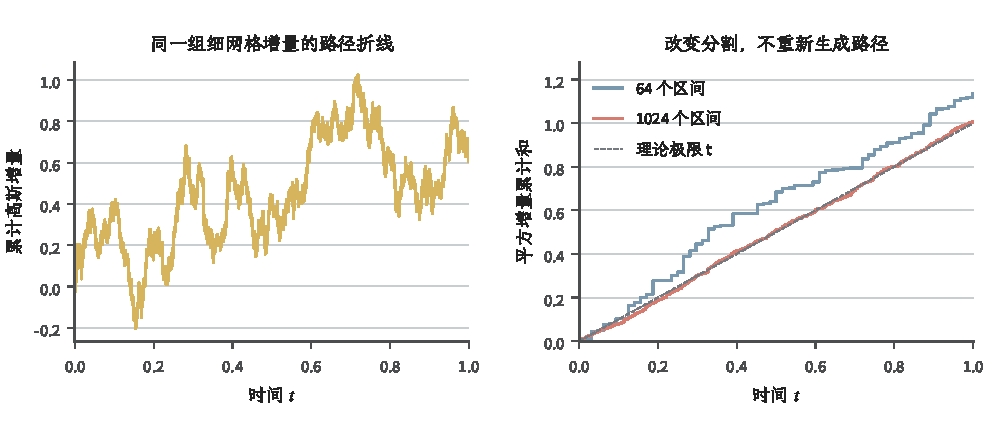
\includegraphics[width=\linewidth]{figures/math-preparation/reader-revision-dynamics/brownian-quadratic-variation.pdf}
  \caption{以固定随机种子构造的高斯增量教学例。左图由$4096$个独立增量
  $\Delta W_i\sim\mathcal N(0,1/4096)$累计成路径折线；右图将同一组增量分别合并为
  $64$和$1024$个时间区间，再累计各区间增量的平方。蓝、红阶梯线使用不同分割，
  灰色参考线为理论二次变差$t$。这里只绘制有限网格，不把某一条折线作为连续布朗路径或收敛证明。}
  \label{fig:reader-brownian-quadratic-variation}
\end{figure*}

平方增量会留下有限的累计量，这使普通积分的链式法则不再适用。接下来先构造只能使用过去信息的随机积分，再用它定义状态方程及其密度演化。

\subsection{可预测过程与Itô积分}

随机积分需要禁止被积量提前使用下一段噪声。可预测性把这项信息限制写成过程的可测条件；
在下面的简单过程中，它表现为每个区间的系数必须在该区间开始时已经知道。
一般可预测过程相对于由左连续适应过程生成的可预测$\sigma$代数可测；
这比逐时刻适应还包含时间方向的联合可测性。先对可预测简单过程定义积分。 给定分割$0=t_{0}<\cdots<t_{n}=T$， 令
\[
	H_{t}= \sum_{i=0}^{n-1}H_{i}\mathbb{I}_{(t_i,t_{i+1}]}(t),
\]
其中$H_{i}$对$\mathcal{F}_{t_i}$可测且平方可积。 定义
\begin{equation}
	\int_{0}^{T}H_{t}\,\mathrm{d}W_{t}:=
	\sum_{i=0}^{n-1}H_{i}(W_{t_{i+1}}-W_{t_i}). \label{eq:dynamical-simple-ito-integral}
\end{equation}
左端点可测性表示$H_{i}$可以依赖过去， 却不能利用尚未发生的布朗增量。

令
\[
	M_t=\int_0^t H_s\,\mathrm{d}W_s
	=\sum_{i=0}^{n-1}H_i
	\left(W_{t\wedge t_{i+1}}-W_{t\wedge t_i}\right).
\]
这个过程对$\mathcal F_t$适应且平方可积。对$0\leq s<t\leq T$，把
$M_t-M_s$按分割区间展开。对包含$s$的区间，系数已经对$\mathcal F_s$可测，
而$s$之后的增量独立于$\mathcal F_s$；对每个起点$t_i\geq s$的完整区间，塔式性质给出
\[
	\mathbb{E}[H_i\Delta W_i\mid\mathcal F_s]
	=
	\mathbb{E}\!\left[
	\mathbb{E}[H_i\Delta W_i\mid\mathcal F_{t_i}]
	\mid\mathcal F_s
	\right]
	=0.
\]
因此
\[
	\mathbb{E}[M_t-M_s\mid\mathcal F_s]=0,
	\qquad
	\mathbb{E}[M_t\mid\mathcal F_s]=M_s.
\]
所以$(M_t)_{0\leq t\leq T}$是平方可积鞅，特别地$\mathbb{E}[M_T]=0$。

等距关系还需要核对平方展开中的交叉项。记
$\Delta W_i=W_{t_{i+1}}-W_{t_i}$。当$i<j$时，
$H_iH_j\Delta W_i$对$\mathcal F_{t_j}$可测，故
\[
	\mathbb{E}[H_iH_j\Delta W_i\Delta W_j]
	=
	\mathbb{E}\!\left[
	H_iH_j\Delta W_i
	\mathbb{E}[\Delta W_j\mid\mathcal F_{t_j}]
	\right]
	=0.
\]
对角项则由$\Delta W_i$独立于$\mathcal F_{t_i}$及其方差
$t_{i+1}-t_i$得到
\[
	\mathbb{E}[H_i^2(\Delta W_i)^2]
	=\mathbb{E}[H_i^2](t_{i+1}-t_i).
\]
将各项相加，得到\term{Itô等距}（Itô isometry）
\begin{equation}
	\mathbb{E}\left[ \left( \int_{0}^{T}H_{t}\,\mathrm{d}W_{t}\right)^{2}\right] = \mathbb{E}
	\int_{0}^{T}H_{t}^{2}\,\mathrm{d}t. \label{eq:dynamical-ito-isometry}
\end{equation}
对可预测过程$H$，若满足 $\mathbb{E}\int_{0}^{T}H_{t}^{2}\,\mathrm{d}t<\infty$，
便可用可预测简单过程在该二阶范数下逼近，并借助等距关系把积分连续延拓。
条件期望是$L^2$压缩映射，因此上述鞅等式也在这个极限下保留：
$M_t=\int_0^tH_s\,\mathrm dW_s$仍是平方可积鞅。
也可以从渐进可测且满足同一平方可积条件的过程出发； 在通常滤过条件下，可取与它
在$\mathbb{P}\otimes\mathrm{d}t$意义下等价的可预测版本，因而得到相同的积分对象。
仅有适应性并不足以保证上述逼近与积分定义成立。

若使用右端点或中点， 被积量会含有当前增量的信息， 极限一般不同。
Stratonovich积分采用对称极限并保留普通链式法则，
Itô积分采用左端适应性并产生二次变差修正。 两种约定都合法，
但模型漂移在二者转换时会改变，不能只换积分符号
\scite{math-oksendal2003sde}

左端点约定还可以用一个有限和看清。记$\Delta W_i=W_{t_{i+1}}-W_{t_i}$，逐项
展开平方得
\[
  W_{t_{i+1}}^2-W_{t_i}^2
  =2W_{t_i}\Delta W_i+(\Delta W_i)^2.
\]
相加后，中间平方项望远镜消去；二次变差又使$\sum_i(\Delta W_i)^2\to T$，于是
$\sum_iW_{t_i}\Delta W_i\to(W_T^2-T)/2$。若改用右端点，相同恒等式给出
$(W_T^2+T)/2$。差别恰好是$T$，即被积量是否含有当前增量所留下的额外相关项。
这也预示下一节的Itô二阶修正，不能用“步长很小”把它删掉。

\subsection{随机微分方程与强解}

先明确多维驱动对象。相对于同一滤过，
$m$维标准布朗运动
$\bm W_t=(W_t^{(1)},\ldots,W_t^{(m)})^\top$
由相互独立的实值标准布朗运动组成。对$0\leq s<t$，增量
$\bm W_t-\bm W_s$独立于$\mathcal F_s$，并满足
\[
	\bm W_t-\bm W_s\sim\mathcal N(\bm0,(t-s)\bm I_m),
	\qquad
	[W^{(i)},W^{(j)}]_t=\delta_{i,j}t.
\]
最后一个等式说明不同分量的交叉二次变差为零，而每个分量的二次变差为$t$。

布朗路径没有普通时间导数，因此下式的微分记号只是一种紧凑写法，真正定义来自积分等式。
\begin{definition}[Itô随机微分方程与强解]
\label{def:dynamical-ito-sde-strong-solution}
$d$维状态由这个$m$维布朗运动驱动时，Itô\term{随机微分方程}（stochastic differential equation, SDE）写成
\begin{equation}
	\mathrm{d}\bm{X}_{t}= \bm{b}(t,\bm{X}_{t})\,\mathrm{d}t + \bm{\sigma}(t,\bm{X}_{t}
	)\,\mathrm{d}\bm{W}_{t}. \label{eq:dynamical-ito-sde}
\end{equation}
其中$\bm{b}:[0,T]\times\mathbb{R}^d\to\mathbb{R}^d$是漂移，
$\bm{\sigma}:[0,T]\times\mathbb{R}^d\to\mathbb{R}^{d\times m}$是扩散系数，二者均联合Borel可测。
它的含义是
\[
	\bm{X}_{t}= \bm{X}_{0}+ \int_{0}^{t}\bm{b}(s,\bm{X}_{s})\,\mathrm{d}s+ \int_{0}
	^{t}\bm{\sigma}(s,\bm{X}_{s})\,\mathrm{d}\bm{W}_{s}.
\]
在给定的滤过概率空间上，$\bm W$是相对于该滤过的布朗运动，初值$\bm X_0$对
$\mathcal F_0$可测。若一个连续过程对由$\bm X_0$与$(\bm W_s)_{0\leq s\leq t}$生成、
完成并取右连续版本的滤过适应，使两个积分都有定义，
并且上式以概率$1$对所有$t\in[0,T]$同时成立，就称它为该方程的\term{强解}
（strong solution）。
\end{definition}
这里的“强”强调解由给定初值与布朗运动的过去生成，无需另添随机信息，而不只指定
解的分布。路径唯一性是指同一空间上使用同一初值和布朗运动的两个适应连续解
几乎必然处处相同。

\begin{theorem}[SDE强解的存在唯一性]
	\label{thm:dynamical-sde-strong-existence}
	设$(\mathcal F_t)_{t\geq0}$满足通常条件，即完备且右连续，
	$\bm W$是相对于该滤过的$m$维标准布朗运动，
	$\bm{X}_0$对$\mathcal{F}_0$可测且
	$\mathbb{E}\lVert\bm{X}_0\rVert_2^2<\infty$。
	设$\bm b$与$\bm\sigma$关于$(t,\bm x)$联合Borel可测。
	若存在常数$L,C$，使对所有$t\in[0,T]$及$\bm{x},\bm{y}\in\mathbb{R}^d$，
	\begin{align*}
		\lVert\bm{b}(t,\bm{x})-\bm{b}(t,\bm{y})\rVert_2
		+\lVert\bm{\sigma}(t,\bm{x})-\bm{\sigma}(t,\bm{y})\rVert_{\mathrm{F}}
		&\leq L\lVert\bm{x}-\bm{y}\rVert_2,\\
		\lVert\bm{b}(t,\bm{x})\rVert_2^2
		+\lVert\bm{\sigma}(t,\bm{x})\rVert_{\mathrm{F}}^2
		&\leq C(1+\lVert\bm{x}\rVert_2^2),
	\end{align*}
	则式~\eqref{eq:dynamical-ito-sde}在$[0,T]$上存在唯一强解，并且
	$\mathbb{E}\sup_{t\leq T}\lVert\bm{X}_t\rVert_2^2<\infty$。
\end{theorem}

证明仍采用Picard迭代，但确定性积分的上界要与Itô等距和鞅最大不等式配合。
在足够短的时间区间上，这些估计使迭代成为二阶过程空间中的压缩；
逐段延拓覆盖$[0,T]$。对两组解作差并使用同样估计，再由Grönwall不等式得到路径唯一性。
线性增长界控制二阶矩并排除有限时间爆炸。若只有局部Lipschitz，以上论证先给出爆炸时刻之前的局部唯一解，
还需额外增长或Lyapunov条件证明爆炸时刻几乎必然大于$T$。

\subsection{Itô公式与二次变差修正}

\begin{theorem}[Itô公式]
	\label{thm:dynamical-ito-formula} 设$\bm{X}_{t}$满足 式~\eqref{eq:dynamical-ito-sde}，
	并令$f(t,\bm{x})$关于$t$一阶连续可微、 关于$\bm{x}$二阶连续可微。 在相应可积条件下，
	\begin{align}
		\mathrm{d}f(t,\bm{X}_{t}) & = \left[ \partial_{t}f + \nabla f^{\top}\bm{b}+ \frac{1}{2}\operatorname{tr}\left( \bm{\sigma}\bm{\sigma}^{\top}\nabla^{2}f \right) \right]\mathrm{d}t \notag \\
		                          & \quad+ \nabla f^{\top}\bm{\sigma}\,\mathrm{d}\bm{W}_{t}, \label{eq:dynamical-ito-formula}
	\end{align}
	其中右侧各函数在$(t,\bm{X}_{t})$处取值。
\end{theorem}

\paragraph{证明路线与关键项。}
先在分割上对 $f(t_{i+1},\bm{X}_{t_{i+1}}) -f(t_{i},\bm{X}_{t_i})$ 作二阶Taylor展开。
状态增量为
\[
	\Delta\bm{X}_{i}
	=\bm{b}_{i}\Delta t_{i}+\bm{\sigma}_{i}\Delta\bm{W}_{i}+\text{高阶余项}.
\]
一阶项产生 $\partial_{t}f\,\Delta t_{i}$、
$\nabla f^{\top}\bm{b}_{i}\Delta t_{i}$ 和
$\nabla f^{\top}\bm{\sigma}_{i}\Delta\bm{W}_{i}$。 二阶项中， $(\Delta t_{i})^{2}$及
$\Delta t_{i}\Delta W_{i}$求和后消失； 而 $\Delta\bm{W}_{i}\Delta\bm{W}_{i}^{\top}$
的和依二次变差趋向$\bm{I}\Delta t_{i}$。 因此留下
\[
		\frac{1}{2}\operatorname{tr}
		(\bm{\sigma}\bm{\sigma}^{\top}\nabla^{2}f)\Delta t_{i}.
\]
完整证明还需先用停时把$\bm{X}$、系数及$f$的导数局部化到有界区域，再以简单可预测过程逼近随机被积项，
并分别证明Taylor余项、漂移和二次变差交叉项在相应概率或$L^{1}$意义下收敛； 最后令停时趋向无穷。
这里给出的展开只说明二阶修正项的来源，不替代这些局部化、逼近与收敛论证。

形式记忆规则
\[
	(\mathrm{d}W_{t})^{2}=\mathrm{d}t, \qquad \mathrm{d}W_{t}\,\mathrm{d}t=0, \qquad
	(\mathrm{d}t)^{2}=0
\]
概括了量级， 但不能替代适应性、可积性与极限证明。

两个基本例子可以核对积分约定。常数被积过程给出
$\int_0^T c\,\mathrm{d}W_t=cW_T$。对$f(x)=x^2$应用Itô公式则有
\[
	W_T^2=2\int_0^T W_t\,\mathrm{d}W_t+T,
	\qquad
	\int_0^T W_t\,\mathrm{d}W_t=\frac{W_T^2-T}{2}.
\]
若误用普通链式法则，就会漏掉由二次变差产生的$-T/2$修正。

\subsection{线性SDE与Ornstein--Uhlenbeck过程}

先考虑确定性系数的向量线性SDE
\[
	\mathrm d\bm X_t
	=(\bm A_t\bm X_t+\bm c_t)\,\mathrm dt
	+\bm G_t\,\mathrm d\bm W_t,
\]
其中$\bm A_t\in\mathbb{R}^{d\times d}$和$\bm c_t\in\mathbb{R}^d$
是确定性的局部可积函数，$\bm G_t\in\mathbb{R}^{d\times m}$是确定性函数且
$\lVert\bm G_t\rVert_{\mathrm F}^2$局部可积，并假设
$\bm X_0\in L^2$。这些条件保证方程有唯一平方可积强解；相应的均值与协方差函数
绝对连续，下面的微分方程对几乎处处的$t$成立。记
\[
	\bm m_t=\mathbb{E}[\bm X_t],\qquad
	\bm P_t=\operatorname{Cov}(\bm X_t).
\]
对积分方程取期望，随机积分的鞅性质给出
\begin{equation}
	\dot{\bm m}_t=\bm A_t\bm m_t+\bm c_t.
	\label{eq:dynamical-linear-sde-mean}
\end{equation}
再令$\widetilde{\bm X}_t=\bm X_t-\bm m_t$，则
$\mathrm d\widetilde{\bm X}_t
=\bm A_t\widetilde{\bm X}_t\,\mathrm dt+\bm G_t\,\mathrm d\bm W_t$。
对矩阵乘积使用Itô公式，
\[
	\begin{aligned}
	\mathrm d(\widetilde{\bm X}_t\widetilde{\bm X}_t^\top)
	={}&
	\left(
	\bm A_t\widetilde{\bm X}_t\widetilde{\bm X}_t^\top
	+\widetilde{\bm X}_t\widetilde{\bm X}_t^\top\bm A_t^\top
	+\bm G_t\bm G_t^\top
	\right)\mathrm dt\\
	&+\bm G_t\,\mathrm d\bm W_t\,\widetilde{\bm X}_t^\top
	+\widetilde{\bm X}_t\,\mathrm d\bm W_t^\top\bm G_t^\top.
	\end{aligned}
\]
取期望后两个随机积分项消失，得到
\begin{equation}
	\dot{\bm P}_t
	=\bm A_t\bm P_t+\bm P_t\bm A_t^\top+\bm G_t\bm G_t^\top.
	\label{eq:dynamical-linear-sde-covariance}
\end{equation}
这两式说明，漂移传播已有均值与协方差，扩散项则持续注入协方差；
它们是离散Kalman预测公式在连续时间中的对应关系。

标量Ornstein--Uhlenbeck过程是上述方程取
$\bm A_t=-\lambda$、$\bm c_t=0$和$\bm G_t=\sigma$的特例：
\begin{equation}
	\mathrm{d}X_{t}= -\lambda X_{t}\,\mathrm{d}t+ \sigma\,\mathrm{d}W_{t}, \qquad \lambda
	>0. \label{eq:dynamical-ou-sde}
\end{equation}
对$\mathrm{e}^{\lambda t}X_{t}$使用Itô公式， 交叉二次变差项因确定性因子有限变差而为零，
得到
\[
	X_{t}= \mathrm{e}^{-\lambda t}X_{0}+ \sigma \int_{0}^{t}\mathrm{e}^{-\lambda(t-s)}
	\,\mathrm{d}W_{s}.
\]
若$X_{0}$与布朗运动独立，
\begin{align}
	\mathbb{E}X_{t}           & = \mathrm{e}^{-\lambda t}\mathbb{E}X_{0}, \label{eq:dynamical-ou-mean}                                                                          \\
	\operatorname{Var}(X_{t}) & = \mathrm{e}^{-2\lambda t}\operatorname{Var}(X_{0}) + \frac{\sigma^{2}}{2\lambda}(1-\mathrm{e}^{-2\lambda t}). \label{eq:dynamical-ou-variance}
\end{align}
第二式由Itô等距得到。 均值衰减到零， 方差却趋向$\sigma^{2}/(2\lambda)$。 随机稳定状态不是所有轨迹收敛到零，
而是阻尼与持续噪声形成平稳分布。当$\sigma\neq0$时，该分布为非退化的
$\mathcal N(0,\sigma^2/(2\lambda))$；当$\sigma=0$时，它退化为$\delta_0$。

也可对$f(x)=x^{2}$用Itô公式：
\[
	\mathrm{d}(X_{t}^{2}) = (-2\lambda X_{t}^{2}+\sigma^{2})\,\mathrm{d}t + 2\sigma
	X_{t}\,\mathrm{d}W_{t}.
\]
取期望后随机积分均值为零， 得到二阶矩ODE， 其解与式~\eqref{eq:dynamical-ou-variance}一致。
若漏掉Itô修正$\sigma^{2}\mathrm{d}t$， 便会错误地预测方差也衰减到零。

\subsection{生成元与Fokker--Planck方程}

路径方程已经说明一个状态如何移动；若只关心分布，则需计算任意光滑读数$\varphi(\bm X_t)$
的平均变化率。生成元把这项短时变化浓缩成作用于$\varphi$的微分算子。
设$\bm a=\bm\sigma\bm\sigma^\top$。对光滑紧支撑测试函数$\varphi$，时刻$t$的生成元为
\begin{definition}[Itô扩散的生成元]
\label{def:dynamical-diffusion-generator}
\[
	(\mathcal{L}_t\varphi)(\bm{x})
	=\bm{b}(t,\bm{x})^{\top}\nabla\varphi(\bm{x})
	+\frac12\operatorname{tr}\!\left(\bm{a}(t,\bm{x})\nabla^2\varphi(\bm{x})\right).
\]
\end{definition}
在系数连续且短时期望允许相应极限交换时，它也等于从$\bm x$出发的
$[\mathbb E_{t,\bm x}\varphi(\bm X_{t+h})-\varphi(\bm x)]/h$在$h\downarrow0$时的极限。
生成元作用于读数函数；Fokker--Planck算子稍后作用于密度，二者通过积分对偶相连。
在Itô公式中的随机积分可积且均值为零时，取期望得到弱演化式
\[
	\frac{\mathrm{d}}{\mathrm{d}t}\mathbb{E}[\varphi(\bm{X}_{t})]
	=\mathbb{E}[(\mathcal{L}_t\varphi)(\bm{X}_t)].
\]
这个等式只描述分布对测试函数的作用，不预设$\bm{X}_t$具有处处光滑的密度。

若$\bm{X}_t$进一步具有密度$p(t,\bm{x})$，且系数与密度足够正则，
便可把弱式写成密度积分并对空间变量分部积分。边界项在测试函数紧支撑，
或密度与通量适当衰减的条件下消失，得到
\begin{equation}
	\partial_{t}p(t,\bm{x}) = - \sum_{i}\partial_{x_i}\bigl(b_{i}(t,\bm{x})p(t,\bm{x}
	)\bigr) + \frac{1}{2}\sum_{i,j}\partial_{x_i}\partial_{x_j}\bigl(a_{i,j}(t, \bm
	{x})p(t,\bm{x})\bigr). \label{eq:dynamical-fokker-planck}
\end{equation}
这就是\term{Fokker--Planck方程}。 它是SDE生成元的伴随方程， 描述各时刻边缘密度怎样流动和扩散。

推导先在弱意义下成立。 要把它解释为逐点经典偏微分方程，
还需密度存在、系数正则性与边界条件。 退化扩散矩阵可能使密度集中在低维集合，
此时相对于全维Lebesgue测度的光滑密度未必存在。

\subsection{SDE数值近似、Langevin与概率流}

Euler--Maruyama方法把 式~\eqref{eq:dynamical-ito-sde}离散为
\begin{equation}
	\bm{X}_{k+1}= \bm{X}_{k}+ \bm{b}(t_{k},\bm{X}_{k})h+ \bm{\sigma}(t_{k},\bm{X}_{k}
	)\sqrt{h}\,\bm{\varepsilon}_{k}, \qquad \bm{\varepsilon}_{k}\sim\mathcal{N}(\bm
	{0},\bm{I}). \label{eq:dynamical-euler-maruyama}
\end{equation}
式中的独立$\bm\varepsilon_k$为$m$维标准高斯。讨论强误差时，必须令
$\sqrt h\,\bm\varepsilon_k=\bm W_{t_{k+1}}-\bm W_{t_k}$，使数值解与真解使用同一个驱动。
对自治系数，若$\bm{b}$与$\bm{\sigma}$全局Lipschitz并满足线性增长条件，且初值平方可积，
则在固定有限时域的网格点上有代表性的强误差界
\[
	\max_{0\leq k\leq T/h}
	\left(\mathbb{E}\lVert\bm{X}_{t_k}-\bm{X}_k\rVert_2^2\right)^{1/2}
	\leq C_T h^{1/2}.
\]
若系数还显式依赖时间，需要相应的时间正则性。一个便于陈述的弱一阶充分条件是：
自治的漂移、扩散系数和测试函数$\varphi$具有至四阶连续有界导数，并满足所需矩条件。此时
\[
	\left|\mathbb{E}\varphi(\bm{X}_T)-\mathbb{E}\varphi(\bm{X}_{T/h})\right|
	\leq C_{\varphi,T}h.
\]
强误差比较同一布朗路径上的数值解与真解，弱误差比较测试函数期望；
两者的对象不同，弱阶更高不表示逐路径更准确。加性噪声或更强结构可以提高特定方法的阶，
但不能把这些特殊结论当作一般乘性噪声的保证。

过阻尼Langevin SDE
\begin{equation}
	\mathrm{d}\bm{X}_{t}= \frac{1}{2}\nabla\log\pi(\bm{X}_{t})\,\mathrm{d}t+ \mathrm{d}
	\bm{W}_{t}\label{eq:dynamical-langevin-sde}
\end{equation}
在$\pi$光滑、可归一化且边界通量消失等条件下， 把$p=\pi$代入Fokker--Planck方程可见漂移通量与扩散通量相消，
所以$\pi$是不变密度。 这只证明保持性。 从任意初值收敛到$\pi$还需要遍历性与约束势能等条件，
离散后的未校正Langevin算法还会产生步长偏差。

扩散生成模型设计随时间加噪的前向SDE， 再学习与边缘分数$\nabla\log p_{t}$有关的反向动态。
与同一边缘密度族对应的概率流ODE可以写成
\[
	\frac{\mathrm{d}\bm{X}_{t}}{\mathrm{d}t}= \bm{b}(t,\bm{X}_{t}) - \frac{1}{2}\bm
	{a}(t) \nabla\log p_{t}(\bm{X}_{t})
\]
这一简式要求扩散矩阵只依赖时间； 状态依赖扩散还会出现额外散度项。
概率流ODE匹配边缘密度演化， 不表示它与SDE具有相同样本路径。
反向生成还需要分数估计与时间反演条件， 不能只凭前向Fokker--Planck方程自动得到。

从单条轨迹转向密度时，控制的对象也改变了。表~\ref{tab:dynamical-path-distribution}
将本节的几种结论放在一起：保持一个分布与从任意初态趋向该分布之间，还隔着长期
混合条件；具有相同边缘密度则连联合路径分布也没有固定。

\begin{table*}[htbp]
  \centering
  \begin{tabularx}{\linewidth}{lXX}
    \toprule
    结论 & 所比较的对象 & 仍需另外说明的对象\\
    \midrule
    强数值误差小 & 同一噪声路径下的数值状态与真状态 & 目标分布的长期抽样偏差\\
    弱数值误差小 & 测试函数在两种状态分布下的期望 & 单条路径之间的距离\\
    密度$\pi$不变 & 若初始分布为$\pi$，以后仍为$\pi$ & 其他初态是否收敛到$\pi$\\
    概率流匹配边缘 & 每个时刻的状态分布 & 时间间联合分布与样本路径\\
    \bottomrule
  \end{tabularx}
  \caption{随机演化中不同结论的对象。强弱误差须满足相应数值方法条件；不变性和边缘
  匹配须满足前述正则性及边界条件。表中各项不能互相替代。}
  \label{tab:dynamical-path-distribution}
\end{table*}

\section{保持保守轨迹的几何结构并构造采样提议}
\label{sec:dynamical-hamiltonian-geometric-integration}

前面的随机微分研究噪声与分布演化。本节回到确定性状态方程，
专门研究具有位置--动量结构的系统：能量守恒和相空间体积保持成为应保留的性质。
几何积分据此设计数值更新；Hamilton蒙特卡洛再加入随机刷新与接受校正，
才能把这种确定性轨迹用于概率采样。它不是由一般SDE直接推出的一项性质。

\subsection{相空间状态与Hamilton方程}

前面主要问扰动是否衰减。 保守系统关心另一类结构：
动态可以长期移动，却保持总能量和相空间体积。
\begin{definition}[可分Hamilton系统]
\label{def:dynamical-separable-hamiltonian-system}
令位置$\bm{q}\in\mathbb{R}^{d}$、动量$\bm{p}\in\mathbb{R}^{d}$，设势能$U$连续可微，
质量矩阵$\bm M\in\mathbb R^{d\times d}$对称正定。可分Hamilton量为
\begin{equation}
	H(\bm{q},\bm{p}) = U(\bm{q})+ \frac{1}{2}\bm{p}^{\top}\bm{M}^{-1}\bm{p}, \qquad
	\bm{M}\succ\bm{0}. \label{eq:dynamical-separable-hamiltonian}
\end{equation}
Hamilton方程为
\begin{equation}
	\dot{\bm{q}}= \nabla_{\bm{p}}H, \qquad \dot{\bm{p}}= -\nabla_{\bm{q}}H. \label{eq:dynamical-hamilton-equations}
\end{equation}
\end{definition}
第一式把动量变成位置速度， 第二式让势能梯度改变动量。 这不是沿$-\nabla H$下降，
而是用辛矩阵
\[
	\bm{J}=
	\begin{bmatrix}
		\bm{0}  & \bm{I} \\
		-\bm{I} & \bm{0}
	\end{bmatrix}
\]
旋转Hamilton梯度。

\subsection{Hamilton流的能量守恒}

\begin{theorem}[Hamilton能量守恒]
	\label{thm:dynamical-hamiltonian-energy-conservation} 若$H$连续可微、不显含时间，
	且Hamilton方程的解在所考察区间存在， 则沿精确轨迹
	\[
		H(\bm{q}(t),\bm{p}(t)) = H(\bm{q}(0),\bm{p}(0)).
	\]
\end{theorem}

\begin{proof}
	沿轨迹使用链式法则，
	\[
		\begin{aligned}
			\frac{\mathrm{d}}{\mathrm{d}t}H & = \nabla_{\bm{q}}H^{\top}\dot{\bm{q}}+ \nabla_{\bm{p}}H^{\top}\dot{\bm{p}}              \\
			                                & = \nabla_{\bm{q}}H^{\top}\nabla_{\bm{p}}H - \nabla_{\bm{p}}H^{\top}\nabla_{\bm{q}}H =0.
		\end{aligned}
	\]
	因此Hamilton量沿每条存在的轨迹保持常数。
\end{proof}

若$H$显式依赖时间， 同一计算只给出
$\mathrm{d}H/\mathrm{d}t=\partial H/\partial t$。 若解在有限时间爆炸， 守恒结论也只适用于流存在的区间。
能量守恒不表示位置有界； 若势能的等能面不紧，轨迹仍可能逃向无穷远。

\subsection{相空间体积与辛结构}

把$\bm{z}=(\bm{q},\bm{p})$， 向量场写成 $\bm{F}(\bm{z})=\bm{J}\nabla H(\bm{z})$。
若$H$二阶连续可微，
\[
	\nabla\cdot\bm{F}= \operatorname{tr}(\bm{J}\nabla^{2}H)=0,
\]
因为$\bm{J}$反对称而$\nabla^{2}H$对称， 二者乘积的迹为零。

设流映射为$\varphi_{t}$， 其Jacobian矩阵为 $\bm{G}_{t}=\nabla\varphi_{t}(\bm{z}_{0})$。
变分方程给出
\[
	\dot{\bm{G}}_{t}= \nabla\bm{F}(\bm{z}(t))\bm{G}_{t}.
\]
Jacobi行列式公式于是给出
\[
	\frac{\mathrm{d}}{\mathrm{d}t}\log|\det\bm{G}_{t}| = \operatorname{tr}(\nabla\bm
	{F}) = \nabla\cdot\bm{F}=0.
\]
由于$\bm{G}_{0}=\bm{I}$， 有$|\det\bm{G}_{t}|=1$。
因此精确Hamilton流保持相空间体积。

体积只记录所有方向伸缩率的乘积，Hamilton系统还保持方向对之间的几何关系。
\begin{definition}[标准辛形式与辛映射]
\label{def:dynamical-symplectic-form-map}
对切向量$\bm{u},\bm{v}\in\mathbb{R}^{2d}$，定义\term{辛形式}（symplectic form）
\[
	\omega(\bm{u},\bm{v})=\bm{u}^{\top}\bm{J}\bm{v}.
\]
可微映射$\psi$称为辛映射，如果其Jacobian矩阵$\bm{G}=\nabla\psi$满足
\begin{equation}
	\bm{G}^{\top}\bm{J}\bm{G}=\bm{J}. \label{eq:dynamical-symplectic-map}
\end{equation}
其中等式在映射定义域的每一点成立，$\psi$为该域到$\mathbb R^{2d}$的连续可微映射。
\end{definition}
该等式表示映射前后的任意两方向具有相同辛形式值。

若$H\in C^2$，沿精确流有
$\nabla\bm{F}=\bm{J}\nabla^2H$。记$\bm{S}=\nabla^2H=\bm{S}^{\top}$，则
\[
	\begin{aligned}
	\frac{\mathrm{d}}{\mathrm{d}t}
	(\bm{G}_t^{\top}\bm{J}\bm{G}_t)
	&=\bm{G}_t^{\top}
	\left[(\bm{J}\bm{S})^{\top}\bm{J}
	+\bm{J}(\bm{J}\bm{S})\right]\bm{G}_t\\
	&=\bm{G}_t^{\top}(\bm{S}-\bm{S})\bm{G}_t=\bm{0}.
	\end{aligned}
\]
初值为$\bm{G}_0^{\top}\bm{J}\bm{G}_0=\bm{J}$，所以精确流满足
式~\eqref{eq:dynamical-symplectic-map}。对该式取行列式可得
$(\det\bm{G}_t)^2=1$；由$\det\bm{G}_0=1$和连续性知$\det\bm{G}_t=1$。
因此辛性蕴含定向体积保持。在一个位置与一个动量组成的二维相空间中，辛形式就是
有向面积形式；但当$d\geq2$时，一般的体积保持映射未必保持辛形式。例如在
$(q_1,q_2,p_1,p_2)$坐标下，$\operatorname{diag}(2,1,1,1/2)$的行列式为$1$，
却把第一对位置动量的面积乘以$2$、第二对乘以$1/2$，不满足
式~\eqref{eq:dynamical-symplectic-map}。总体积不变不能替代每对共轭方向的结构保持。

\subsection{分裂积分与蛙跳方法}

对可分Hamilton量~\eqref{eq:dynamical-separable-hamiltonian}， 一步步长为$h$的蛙跳积分写成
\begin{align}
	\bm{p}_{k+1/2} & = \bm{p}_{k}- \frac{h}{2}\nabla U(\bm{q}_{k}), \label{eq:dynamical-leapfrog-half-momentum}        \\
	\bm{q}_{k+1}   & = \bm{q}_{k}+ h\bm{M}^{-1}\bm{p}_{k+1/2}, \label{eq:dynamical-leapfrog-position}                  \\
	\bm{p}_{k+1}   & = \bm{p}_{k+1/2}- \frac{h}{2}\nabla U(\bm{q}_{k+1}). \label{eq:dynamical-leapfrog-final-momentum}
\end{align}
两次动量剪切和一次位置剪切都具有Jacobian矩阵的行列式$1$， 所以复合映射体积保持。 把$h$换成$-
h$并反向执行三步， 可以精确恢复起点， 所以映射具有时间可逆性。 它还是辛积分器， 因为每个子步都是一个Hamilton子流。

这些性质可以直接从Jacobian核对。动量剪切
$S_U^c(\bm{q},\bm{p})=(\bm{q},\bm{p}-c\nabla U(\bm{q}))$与位置剪切
$S_K^h(\bm{q},\bm{p})=(\bm{q}+h\bm{M}^{-1}\bm{p},\bm{p})$的Jacobian分别为
\[
	\bm{G}_U=
	\begin{bmatrix}
		\bm{I}&\bm{0}\\
		-c\nabla^2U&\bm{I}
	\end{bmatrix},
	\qquad
	\bm{G}_K=
	\begin{bmatrix}
		\bm{I}&h\bm{M}^{-1}\\
		\bm{0}&\bm{I}
	\end{bmatrix}.
\]
由于$\nabla^2U$与$\bm{M}^{-1}$对称，直接相乘可得
$\bm{G}_U^{\top}\bm{J}\bm{G}_U=\bm{J}$和
$\bm{G}_K^{\top}\bm{J}\bm{G}_K=\bm{J}$。
蛙跳映射是$S_U^{h/2}\circ S_K^h\circ S_U^{h/2}$，而辛映射的复合仍为辛映射。
每个三角Jacobian的行列式为$1$，也再次给出体积保持。

令动量翻转为$R(\bm{q},\bm{p})=(\bm{q},-\bm{p})$，并记一步蛙跳为$\Psi_h$。
三步的对称排列给出
\[
	R\circ\Psi_h\circ R=\Psi_h^{-1}=\Psi_{-h}.
\]
所以可逆性不是简单的$\Psi_h=\Psi_h^{-1}$，而是在反向运动时同时翻转动量。

蛙跳法一般不精确保持原Hamilton量。 它对固定有限时间具有二阶全局精度，
并在合适光滑和步长条件下近似保持一个修正Hamilton量，
所以长时间能量误差常表现为有界振荡，而非单向漂移。
“可逆”“体积保持”“辛”和“能量误差小”是相关但不同的性质；
验证其中一项不能自动推出其余各项。

\begin{example}[谐振子的精确与数值轨道]
	\label{ex:dynamical-harmonic-oscillator} 取$U(q)=q^{2}/2$、$M=1$。 Hamilton方程为
	\[
		\dot q=p,\qquad \dot p=-q,
	\]
	精确轨迹沿圆 $q^{2}+p^{2}=\text{常数}$旋转。蛙跳一步可写成
	\[
		\begin{bmatrix}q_{k+1}\\p_{k+1}\end{bmatrix}
		=
		\begin{bmatrix}
			1-h^2/2 & h\\
			-h+h^3/4 & 1-h^2/2
		\end{bmatrix}
		\begin{bmatrix}q_k\\p_k\end{bmatrix}.
	\]
	该矩阵行列式为$1$、迹为$2-h^2$。其特征值在单位圆上且不退化的条件是
	$|2-h^2|<2$，即$0<h<2$。在这个稳定范围内，数值轨迹沿接近圆的闭曲线运动，
	原能量会有小幅周期误差； 步长过大时，即使每一步仍可逆且行列式为$1$，
	轨迹也可能不稳定。 几何结构保持不能替代步长稳定性检查。
\end{example}

\subsection{Hamilton蒙特卡洛与接受校正}

若目标密度满足 $\pi(\bm{q})\propto\exp[-U(\bm{q})]$， 再引入高斯动量
$\bm{p}\sim \mathcal{N}(\bm{0},\bm{M})$， 联合密度正比于 $\exp[-H(\bm{q},\bm{p})]$。
精确Hamilton流同时保持$H$和体积， 因而保持该联合密度。 数值蛙跳产生候选
$(\bm{q}',\bm{p}')$时存在能量误差
\[
	\Delta H = H(\bm{q}',\bm{p}')-H(\bm{q},\bm{p}).
\]
Metropolis接受概率
\begin{equation}
	a = \min\{1,\exp(-\Delta H)\} \label{eq:dynamical-hmc-acceptance}
\end{equation}
结合可逆、体积保持的提议映射， 恢复对目标联合分布的详细平衡。 拒绝时保留原位置， 动量翻转用于明确反向提议。

更具体地，令$\rho(\bm{z})\propto\exp[-H(\bm{z})]$，把若干步蛙跳与末端动量翻转合成映射
$T$。上面的可逆性给出$T(T(\bm{z}))=\bm{z}$，体积保持给出
$|\det\nabla T|=1$。于是成对状态间的接受概率满足
\[
	\rho(\bm{z})\min\!\left\{1,\frac{\rho(T\bm{z})}{\rho(\bm{z})}\right\}
	=\min\{\rho(\bm{z}),\rho(T\bm{z})\}
	=\rho(T\bm{z})\min\!\left\{1,\frac{\rho(\bm{z})}{\rho(T\bm{z})}\right\}.
\]
这就是确定性提议上的详细平衡；Jacobian若不为$1$，接受比还必须包含相应体积因子。
每轮重新抽取服从$\mathcal{N}(\bm{0},\bm{M})$的动量也保持联合目标密度，
边缘化动量后才得到位置目标$\pi(\bm{q})$。

接受校正保证的是不变分布， 不是独立样本、快速混合或有限预算精度。
步长太大会导致频繁拒绝， 轨迹太短会导致高自相关，
质量矩阵不合适会使不同方向的时间尺度失配。
另一方面，Hamilton轨迹不要求能量持续下降。
采样希望沿等能面远距离移动后保持目标分布， 优化则希望找到低目标值；
把Hamilton动力学解释成“更快的梯度下降”会混淆这两个目标。

\section{本章小结}
\label{sec:dynamical-systems-state-estimation-summary}

状态把过去对未来的作用压缩进当前变量。 给定初值与输入，差分方程直接生成递推，
常微分方程通过流映射生成连续轨迹。 局部Lipschitz条件保证局部唯一解，
全局解还需要增长或有界性控制。 线性时不变系统可用矩阵指数求解，
时变系统则需要保留状态转移矩阵的时间顺序。

离散化近似连续流。 Euler、Runge--Kutta与零阶保持的误差来源不同，
连续系统稳定也不保证任意步长的数值递推稳定。 仿射更新的结合律允许前缀扫描，
却不允许交换时间次序。 稳定性同样要区分平衡点不离开、轨迹趋近平衡和输入作用。
谱决定线性系统的长期行为， Lyapunov函数把更一般的稳定性转成标量下降，
非正规系统则提醒我们长期衰减可以伴随短时放大。

加入过程噪声后，状态方程传播分布； 加入观测噪声后，观测历史通过条件化形成滤波分布。
在线性高斯及独立噪声条件下， Kalman递推由一次联合高斯条件化精确得到， RTS递推再利用未来观测修正过去边缘。
这些是有限时域结论。 稳态增益和极限协方差还需要第~\ref{chap:control-theory}章建立的可检测性等系统条件，
非线性或非高斯模型也需要明确近似对象。

随机参数递推的平均ODE只描述平均方向。
非对称线性漂移应检查特征值实部、对称部分或Lyapunov方程，
不能把一般漂移矩阵当作目标Hessian矩阵。 同策略线性TD的加权Markov收缩可给出稳定漂移，
离策略分布改变后必须重新证明。 平均稳定仍不能替代步长、噪声、混合和迭代有界性。

连续时间噪声具有平方根增量和非零二次变差。 这使布朗路径不能作为普通可微输入， 并使Itô公式保留二阶修正。
SDE描述随机路径， Fokker--Planck方程描述边缘密度， Euler--Maruyama的强弱误差又是数值近似性质。
Hamilton动力学则保持能量与相空间几何； 蛙跳的可逆和体积保持帮助构造采样提议， 但不等于精确守恒，也不等于优化下降。

由此，章首问题可以分成两部分回答： 状态方程和噪声条件决定轨迹或分布怎样演化，
观测历史和条件化规则决定能够推断什么。 第~\ref{chap:decision-theory-and-dynamic-risk}章将在这些动态之上评价行动后果，
第~\ref{chap:control-theory}章再让输入由反馈主动选择，
并建立稳态估计、最优控制与安全约束所需的结构条件。

\chapter{决策理论与动态风险}
\label{chap:decision-theory-and-dynamic-risk}

第~\ref{chap:dynamical-systems-and-state-estimation}章说明了给定输入后状态怎样演化，
第~\ref{chap:probability-theory}章则说明给定观测后可以怎样更新结果分布。
但分布本身不会告诉我们应该采取什么行动。即使两个分类器给出完全相同的患病概率，
筛查系统与确诊系统也可能采用不同阈值，因为漏诊和误报的后果不同。决策需要在概率
之外再给出行动集合和损失，并说明怎样汇总随机后果。

当行动还会改变下一时刻的状态时，单步比较又不够。当前多付一点成本，可能换来以后
更好的状态或更有用的信息；当前平均成本较低，也可能隐藏小概率的严重损失。本章由
单步Bayes决策建立“分布加损失”的共同语言，再比较均值、分位数、条件风险价值和
鲁棒目标各自在评价什么。随后把行动放入有限状态的动态过程，从条件期望推导有限时域
与折扣动态规划，并用线性规划对偶连接价值函数和占用流量。

信息价值和动态风险从两个方向扩展这一基准。前者问提前获得一项观测能否改变后续行动，
后者问在每个历史下应怎样评价剩余损失。静态尾部准则、嵌套条件风险和最坏模型递推
可能使用相似的优化式，却不一定定义同一个目标。贯穿本章的判断原则是：先写清随机
对象、可用信息和允许行动，再检查所用风险准则能否与时间递推相容。

\section{把预测分布转化为有代价的行动}
\label{sec:decision-bayes-rules}

\subsection{损失函数、条件风险与Bayes规则}
设观测为\(X\)，未知结果为\(Y\in\mathcal{Y}\)，可选行动属于
\(\mathcal{A}\)。损失函数
\[
  \ell:\mathcal{A}\times\mathcal{Y}\to\mathbb{R}
\]
规定结果为\(y\)时采取行动\(a\)要付出多少代价。给定\(X=x\)以后，结果仍然
不确定，因此需要把每个可能结果的代价按条件概率汇总。
\begin{definition}[条件风险与Bayes决策]
\label{def:decision-conditional-risk-bayes-rule}
给定条件分布核$P(\mathrm dy\mid x)$，假设损失可测，以下出现的期望均有限。各行动的
\term{条件风险}（conditional risk）为
\begin{equation}
  r(a\mid x)
  =
  \mathbb{E}[\ell(a,Y)\mid X=x].
  \label{eq:decision-conditional-risk}
\end{equation}
若条件分布以概率核给出，式~\eqref{eq:decision-conditional-risk}就是
\[
  r(a\mid x)
  =
  \int_{\mathcal{Y}}\ell(a,y)P(\mathrm{d}y\mid x).
\]
有限类别时，积分退化为
\(\sum_y\ell(a,y)p(y\mid x)\)。

在条件风险达到最小值时，任取
\begin{equation}
  a^\star(x)
  \in
  \argmin_{a\in\mathcal{A}}r(a\mid x)
  \label{eq:decision-bayes-action}
\end{equation}
称为一个\term{Bayes行动}（Bayes action），映射
\(\delta^\star:x\mapsto a^\star(x)\)称为\term{Bayes决策规则}
（Bayes decision rule），其中该逐点选择须可测。
\end{definition}
这里的“Bayes”指按照给定条件分布最小化后验期望
损失。条件分布可以来自先验与似然的更新，也可以由其他概率模型给出；Bayes公式负责
更新信念，Bayes规则负责把信念转成行动，两者不是同一步。

若决策规则为\(\delta\)，其总体风险为
\begin{equation}
  R(\delta)
  =
  \mathbb{E}[\ell(\delta(X),Y)].
  \label{eq:decision-rule-risk}
\end{equation}
全期望公式给出
\[
  R(\delta)
  =
  \mathbb{E}\bigl[r(\delta(X)\mid X)\bigr].
\]
因此，只要式~\eqref{eq:decision-bayes-action}中的逐点最小值可测地选取，
\(r(\delta^\star(x)\mid x)\leq r(\delta(x)\mid x)\)便在积分后推出
\(R(\delta^\star)\leq R(\delta)\)。有限行动集合中可按固定次序处理并列，
可测选择没有额外困难；一般行动空间还要核对损失的可测性、下半连续性以及最小值
是否达到。

\begin{example}[有限损失表的逐项计算]
\label{ex:decision-finite-loss-table}
设结果\(Y\in\{y_0,y_1\}\)，两个行动的损失表为
\[
  \begin{array}{c|cc}
    &y_0&y_1\\ \hline
    a_0&0&6\\
    a_1&2&1
  \end{array}
\]
在某个观测\(x\)处，设
\(\mathbb{P}(Y=y_1\mid X=x)=1/4\)。于是
\[
  r(a_0\mid x)
  =
  \frac34\times0+\frac14\times6
  =
  \frac32,
  \qquad
  r(a_1\mid x)
  =
  \frac34\times2+\frac14\times1
  =
  \frac74.
\]
Bayes行动是\(a_0\)，因为它比较的是按条件概率加权后的整行损失，而不是逐列挑选
较小数字。若结果扩展为有限集合\(\{y_1,\ldots,y_m\}\)，同一计算变成
\(r(a\mid x)=\sum_{j=1}^m\ell(a,y_j)
\mathbb{P}(Y=y_j\mid X=x)\)。
\end{example}

这个逐点选择确实给出总体最优，而不只是局部启发式。对任意使用同一观测\(X\)的
可测规则\(\delta\)，塔式法则和逐点最小性依次给出
\begin{align*}
  R(\delta^\star)
  &=
  \mathbb{E}\left[
    \mathbb{E}\{\ell(\delta^\star(X),Y)\mid X\}
  \right]\\
  &=
  \mathbb{E}\left[\min_{a\in\mathcal{A}}r(a\mid X)\right]
  \leq
  \mathbb{E}\left[r(\delta(X)\mid X)\right]
  =
  R(\delta).
\end{align*}
这里要求各项期望存在；有限行动保证可以按固定次序选取第一个最小行动。若
\(\mathcal{A}\)连续，\(\inf_a r(a\mid x)\)可能不达到，逐点最优行动也可能无法
可测地拼成规则，因而不能直接沿用有限集合的结论。

\subsection{代价敏感分类与决策阈值}
考虑二分类\(Y\in\{0,1\}\)与预测行动\(a\in\{0,1\}\)。记
\[
  p(x)=\mathbb{P}(Y=1\mid X=x),
\]
并设正确预测的损失为零，把假阳性的损失记为\(c_{\mathrm{FP}}>0\)，
假阴性的损失记为\(c_{\mathrm{FN}}>0\)。两个行动的条件风险分别为
\begin{align}
  r(1\mid x)
  &=
  c_{\mathrm{FP}}\bigl(1-p(x)\bigr),
  \label{eq:decision-binary-risk-positive}\\
  r(0\mid x)
  &=
  c_{\mathrm{FN}}p(x).
  \label{eq:decision-binary-risk-negative}
\end{align}
选择\(a=1\)当且仅当第一项不大于第二项，即
\begin{equation}
  p(x)
  \geq
  \frac{c_{\mathrm{FP}}}
       {c_{\mathrm{FP}}+c_{\mathrm{FN}}}.
  \label{eq:decision-cost-sensitive-threshold}
\end{equation}
在等号处两个行动风险相同，可以按业务约定处理并列。

若两类错误代价相同，阈值是\(1/2\)。漏诊代价增大时，
式~\eqref{eq:decision-cost-sensitive-threshold}的阈值下降，系统会更愿意
预测阳性。概率模型没有发生变化，变化的是概率进入行动比较的方式。这也说明概率校准
和决策质量不能互相替代：校准良好的\(p(x)\)仍需配合正确损失，错误的损失设定则会把
准确概率转成不合适的行动。

\begin{example}[同一概率对应不同合理行动]
\label{ex:decision-same-probability-different-actions}
设某个样本的阳性概率为\(p(x)=0.3\)。在对称零一损失下，阈值为\(0.5\)，
Bayes行动是预测阴性。若漏诊损失为\(9\)，误报损失为\(1\)，阈值降为
\(1/(1+9)=0.1\)，同一概率对应的Bayes行动改为预测阳性。这个教学数值没有说明
哪组代价适合真实任务；它只展示决策规则还依赖概率之外的价值判断。
\end{example}

图~\ref{fig:decision-cost-thresholds}把条件风险当作概率$p$的函数。
Bayes规则在两条曲线中选择较低者，交点就是阈值。漏诊成本增大后，预测阴性的风险
上升得更快，交点向较小的$p$移动；这使“更谨慎”的含义得到明确解释：谨慎针对哪一种
错误，决定了阈值应向哪个方向改变。

\begin{figure*}[htbp]
  \centering
  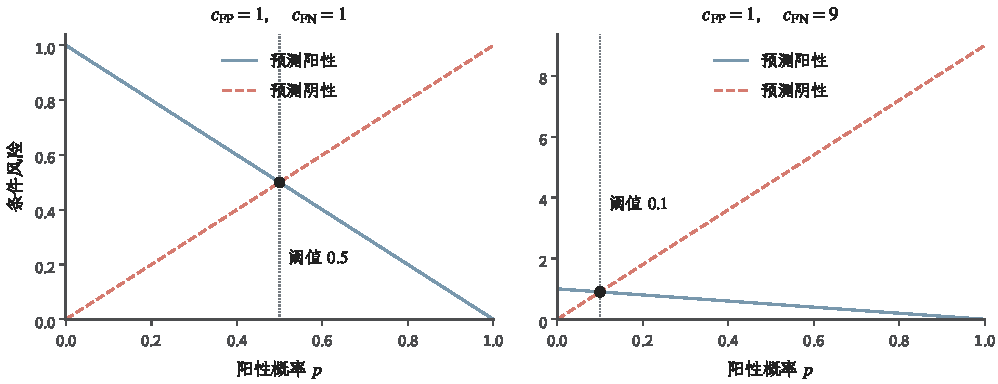
\includegraphics[width=\linewidth]{figures/math-preparation/dynamics/cost-thresholds.pdf}
  \caption{二分类中的条件风险。蓝色实线为预测阳性的风险$c_{\mathrm{FP}}(1-p)$，
  红色虚线为预测阴性的风险$c_{\mathrm{FN}}p$。左图两种错误成本均为$1$，阈值为$0.5$；
  右图仅将漏诊成本增至$9$，阈值降为$0.1$。两图使用相同横轴，纵轴明确显示各自的
  损失范围；教学成本用于说明损失设定如何改变行动。}
  \label{fig:decision-cost-thresholds}
\end{figure*}

\subsection{拒答决策与选择性风险}
模型不确定时，系统可以把样本交给人工复核，而不是被迫给出类别。令类别集合为
\(\{1,\ldots,K\}\)，分类错误使用零一损失，并增加拒答行动
\(\bot\)，其固定损失为\(c_{\mathrm{R}}\in(0,1)\)。若
\[
  p_{\max}(x)=\max_{k}\mathbb{P}(Y=k\mid X=x),
\]
预测最可能类别的条件风险为\(1-p_{\max}(x)\)，拒答风险为
\(c_{\mathrm{R}}\)。因此最优规则为
\begin{equation}
  \delta^\star(x)
  =
  \begin{cases}
    \argmax_k\mathbb{P}(Y=k\mid X=x),
      & p_{\max}(x)\geq1-c_{\mathrm{R}},\\
    \bot,
      & p_{\max}(x)<1-c_{\mathrm{R}}.
  \end{cases}
  \label{eq:decision-reject-rule}
\end{equation}
拒答不是概率模型中的新类别，而是一项具有自身代价的行动。

为描述选择性预测的整体表现，定义\term{覆盖率}（coverage）
\[
  \operatorname{Coverage}(\delta)
  =
  \mathbb{P}\{\delta(X)\neq\bot\},
\]
并在覆盖率为正时定义接受样本上的条件风险
\[
  R_{\mathrm{acc}}(\delta)
  =
  \mathbb{E}\left[
    \ell(\delta(X),Y)
    \,\middle|\,
    \delta(X)\neq\bot
  \right].
\]
低接受风险可以通过拒绝更多样本获得，所以报告它时必须同时报告覆盖率。固定拒答成本
最小化的是包含拒答损失的总体风险，并不等同于在任意指定覆盖率下直接最小化
\(R_{\mathrm{acc}}\)。

若人工复核数量有限，就不能逐个样本独立使用固定
\(c_{\mathrm{R}}\)。例如要求总体接受率至少为\(\kappa\)，可写成
\[
  \min_{\delta}R(\delta)
  \quad\text{s.t.}\quad
  \mathbb{P}\{\delta(X)\neq\bot\}\geq\kappa.
\]
拉格朗日乘子把覆盖预算转成拒答的影子价格，在适当条件下仍得到阈值规则，但阈值由
总体分布和预算共同决定。这类\term{选择性预测}（selective prediction）控制的是
在哪些输入上行动；它不等同于简单提高某个类别的错误代价。

\begin{example}[覆盖预算耦合两个观测点]
\label{ex:decision-two-point-coverage-budget}
设\(X\)等概率取\(x_1,x_2\)，在两个点上作最优分类的条件错误风险分别为
\(0.2\)和\(0.4\)，拒答损失均为\(0.1\)。若逐点比较，两个点都会拒答，因为
\(0.1<0.2<0.4\)，所得覆盖率为零。现在要求
\(\operatorname{Coverage}(\delta)\geq1/2\)，规则至少要接受一个点。接受\(x_1\)并拒答
\(x_2\)的总体风险为
\[
  \frac12\times0.2+\frac12\times0.1=0.15,
\]
反向安排的风险为
\(\frac12\times0.1+\frac12\times0.4=0.25\)。预算把两个观测点的选择联系起来，
最优规则必须联合安排，而不能继续执行原来的逐点拒答。
\end{example}

在有限观测和行动问题中，若允许对每个观测随机选择行动，便可用选择概率作为变量，
把风险与覆盖约束写成线性规划，强对偶给出相应影子价格。若只允许确定性规则，选择
变量带有零一约束，问题一般会变成整数规划，普通线性规划的强对偶不能直接套用。
连续分布或非凸策略类中，拉格朗日形式是否达到原约束问题的值，还要核对可行性、闭性和
相应约束资格；不能仅凭乘子写法断言存在无间隙的阈值解。

\subsection{随机化决策与线性风险}
给定\(x\)，若允许按概率核\(q(\mathrm{d}a\mid x)\)随机选择行动，则条件风险为
\[
  \int_{\mathcal{A}}r(a\mid x)q(\mathrm{d}a\mid x)
  \geq
  \inf_{a\in\mathcal{A}}r(a\mid x).
\]
有限或可数行动集合中，这个积分就是
\(\sum_{a\in\mathcal{A}}q(a\mid x)r(a\mid x)\)。它是各纯行动风险的加权平均，
所以在没有额外耦合约束时，随机化不可能低于纯行动风险的下确界；当最小值达到时，
它至多在多个Bayes行动并列时保持最优。但若不同输入共享总体预算、公平约束或资源约束，
随机化可以精确满足一个纯规则无法达到的平均比例。此时它的作用来自可行域，不是来自
期望损失本身偏好随机行动。

单步Bayes规则由行动、条件分布和损失三者共同确定。接下来保持行动及其随机损失不变，
转而改变汇总随机后果的准则，考察平均损失之外还可以控制什么。

\section{区分平均后果、严重尾部与模型不确定性}
\label{sec:decision-risk-criteria-robustness}

\subsection{期望、方差与风险性质}
本节统一采用“损失越小越好”的方向。设随机损失\(L\)可积。期望
\(\mathbb{E}[L]\)把所有结果按概率线性平均，便于比较和递推，但它可能掩盖稀有而
严重的后果。考虑两个教学方案
\[
  L_{\mathrm{safe}}=1,
  \qquad
  L_{\mathrm{tail}}
  =
  \begin{cases}
    0,&\text{概率 }0.95,\\
    20,&\text{概率 }0.05.
  \end{cases}
\]
两者期望损失都为\(1\)，但第一个方案没有波动，第二个方案把全部平均损失集中到了
最差\(5\%\)的结果中。若任务不能承受这种尾部，单看均值就没有表达完整偏好。

方差\(\operatorname{Var}(L)\)衡量围绕均值的二次波动，均值--方差准则可以写成
\[
  \mathbb{E}[L]+\lambda\operatorname{Var}(L),
  \qquad \lambda\geq0.
\]
它同时惩罚高于和低于均值的偏离；对损失而言，意外变好也会增加方差。此外，方差不是
单调风险准则：即使\(L_1\leq L_2\)逐点成立，较大的\(L_2\)也可能因方差更小而得到
较低的均值--方差值。因此使用它时，应把“波动偏好”和“坏尾部偏好”分开说明。

风险准则的性质说明它怎样响应损失变化。平均损失与尾部损失可以相差很大，但至少应
核对“逐点损失变大，风险会不会反而变小”。以下性质规定的是同一概率空间上损失的比较。
\begin{definition}[相干风险]
\label{def:decision-coherent-risk}
设风险泛函$\rho:L^1(P)\to\mathbb R$。单调性要求对任意$L,L'\in L^1(P)$，
\(L\leq L'\)几乎处处时\(\rho(L)\leq\rho(L')\)；平移等变性要求确定增加
\(m\)单位损失时\(\rho(L+m)=\rho(L)+m\)；凸性要求
\[
  \rho(\tau L+(1-\tau)L')
  \leq
  \tau\rho(L)+(1-\tau)\rho(L'),
  \qquad 0\leq\tau\leq1,
\]
表示按同一场景逐点混合两项损失不会比风险值的同权平均更坏。若再有正齐次性和
次可加性，即$\rho(\lambda L)=\lambda\rho(L)$对$\lambda\geq0$成立，以及
$\rho(L+L')\leq\rho(L)+\rho(L')$，便得到后文使用的\term{相干风险}（coherent risk measure）。
\end{definition}
正齐次与次可加性已经蕴含上述凸性；列出凸性是为了同时说明它与一般凸风险的关系。
这里混合的是同一场景下两项损失的加权和，并非先随机选择某个方案再观察它的损失。
期望满足这些性质。均值--方差准则至少要求
二阶矩存在，并且一般不单调：令\(L_1\)以相同概率取\(0,2\)，令\(L_2=2\)，则
\(L_1\leq L_2\)，但当\(\lambda>1\)时，
\(\mathbb{E}[L_1]+\lambda\operatorname{Var}(L_1)=1+\lambda>2\)，反而把逐点不大的
\(L_1\)评得更差。

\subsection{分位数与风险价值}
\begin{definition}[风险价值]
\label{def:decision-value-at-risk}
对实值随机损失$L$和\(\alpha\in(0,1)\)，其左\(\alpha\)分位数定义为
\begin{equation}
  q_\alpha(L)
  =
  \inf\{z\in\mathbb{R}:\mathbb{P}(L\leq z)\geq\alpha\}.
  \label{eq:decision-loss-quantile}
\end{equation}
在风险管理语境中，同一个量常称为\term{风险价值}
（value at risk, VaR），记作
\(\operatorname{VaR}_{\alpha}(L)=q_\alpha(L)\)。
\end{definition}
它回答“至少\(\alpha\)比例的结果不超过哪一损失水平”。VaR只记录一个切点，
不区分切点以上的损失究竟略高还是极其严重。

在上面的教学例子中，
\[
  \operatorname{VaR}_{0.95}(L_{\mathrm{safe}})=1,
  \qquad
  \operatorname{VaR}_{0.95}(L_{\mathrm{tail}})=0.
\]
按照本书采用的左分位数定义，第二个等式来自
\(\mathbb{P}(L_{\mathrm{tail}}\leq0)=0.95\)。这并不表示尾部方案更安全，
而是表明分位点恰好落在概率质量为\(0.95\)的零损失原子上。离散分布中的边界质量
必须进入尾部计算。

VaR单调且平移等变，却不普遍满足次可加性。设互斥事件\(E_1,E_2\)各有概率
\(0.04\)，令\(L_i=\mathbb{I}\{E_i\}\)。在\(\alpha=0.95\)时，
\(\operatorname{VaR}_{0.95}(L_1)=\operatorname{VaR}_{0.95}(L_2)=0\)，但
\(L_1+L_2\)以概率\(0.08\)取\(1\)，故
\[
  \operatorname{VaR}_{0.95}(L_1+L_2)=1
  >
  \operatorname{VaR}_{0.95}(L_1)
  +
  \operatorname{VaR}_{0.95}(L_2).
\]
两个单独看来未进入最坏\(5\%\)的事件，合并后超过了分位概率预算。这一反例针对
一般分布；在额外分布结构下，VaR仍可能具有更好的性质。

\subsection{条件风险价值与尾部质量}
\term{条件风险价值}（conditional value at risk, CVaR）不只看尾部起点，
还平均最坏的\(1-\alpha\)概率质量\scite{math-rockafellar2000cvar}
\begin{definition}[条件风险价值]
\label{def:decision-conditional-value-at-risk}
对$L\in L^1(P)$和$\alpha\in(0,1)$，定义
\begin{equation}
  \operatorname{CVaR}_{\alpha}(L)
  =
  \inf_{\eta\in\mathbb{R}}
  \left\{
    \eta+
    \frac{1}{1-\alpha}
    \mathbb{E}\bigl[(L-\eta)_+\bigr]
  \right\},
  \qquad
  (u)_+=\max\{u,0\}.
  \label{eq:decision-cvar-optimization}
\end{equation}
\end{definition}
参数\(\eta\)是候选尾部阈值。提高\(\eta\)会直接增加第一项，却会减少超过阈值的
剩余损失；最优点在两种变化之间平衡。

记式~\eqref{eq:decision-cvar-optimization}中花括号内的函数为
\(\phi(\eta)\)。对\(h>0\)，逐点考察正部函数可得
\begin{align*}
  \phi'_+(\eta)
  &=
  1-\frac{\mathbb{P}(L>\eta)}{1-\alpha},\\
  \phi'_-(\eta)
  &=
  1-\frac{\mathbb{P}(L\geq\eta)}{1-\alpha}.
\end{align*}
\(\phi\)是凸函数，所以\(\eta\)最优当且仅当
\[
  \phi'_-(\eta)\leq0\leq\phi'_+(\eta),
\]
也就是
\begin{equation}
  \mathbb{P}(L<\eta)
  \leq\alpha
  \leq
  \mathbb{P}(L\leq\eta).
  \label{eq:decision-cvar-quantile-condition}
\end{equation}
因此任一满足条件的\(\alpha\)分位数都可作为最优阈值。这个推导也解释了为何离散
原子不能直接丢掉：最优阈值处的左右导数可能不同。

令\(q=q_\alpha(L)\)。由
\(\mathbb{P}(L>q)\leq1-\alpha\)及
\(\mathbb{P}(L\geq q)\geq1-\alpha\)，式
\eqref{eq:decision-cvar-optimization}可改写为
\begin{equation}
  \operatorname{CVaR}_{\alpha}(L)
  =
  \frac{
    \mathbb{E}[L\mathbb{I}\{L>q\}]
    +
    q\bigl((1-\alpha)-\mathbb{P}(L>q)\bigr)
  }{1-\alpha}.
  \label{eq:decision-cvar-atomic-tail}
\end{equation}
第二项从\(L=q\)的原子中补足尾部质量。当
\(\mathbb{P}(L\geq q)=1-\alpha\)时，式
\eqref{eq:decision-cvar-atomic-tail}可简写成
\(\mathbb{E}[L\mid L\geq q]\)；分布在\(q\)处连续是保证该等式成立的常见充分条件，
却不是必要条件。无条件使用这个条件期望公式，会在离散分布中平均过多概率质量。

对\(L_{\mathrm{safe}}\)，式~\eqref{eq:decision-cvar-atomic-tail}给出
\(\operatorname{CVaR}_{0.95}=1\)。对\(L_{\mathrm{tail}}\)，最差\(5\%\)
恰好全部位于损失\(20\)，所以
\[
  \operatorname{CVaR}_{0.95}(L_{\mathrm{tail}})=20.
\]
期望看不出两者差异，VaR又在原子边界上给出\(0\)，CVaR则直接反映严重尾部。

\begin{example}[分位点原子中的部分尾部]
  \label{ex:decision-cvar-partial-atom}
  设$L$以概率$0.6,0.3,0.1$分别取$0,2,10$，并取$\alpha=0.75$。
  因为$P(L<2)=0.6<0.75\leq P(L\leq2)=0.9$，分位点为$2$。
  最坏$25\%$由损失$10$的全部$10\%$质量，以及损失$2$的部分$15\%$质量组成，所以
  \[
    \operatorname{CVaR}_{0.75}(L)
    =\frac{0.1\times10+0.15\times2}{0.25}=5.2.
  \]
  直接对事件$L\geq2$条件化会平均$40\%$的质量，得到
  $(0.3\times2+0.1\times10)/0.4=4$，不是此处的CVaR。
  图~\ref{fig:decision-cvar-threshold}同时展示阈值优化式的最低点：阈值前后斜率
  改变，正好对应分位点处需要取部分原子质量。
\end{example}

\begin{figure}[htbp]
  \centering
  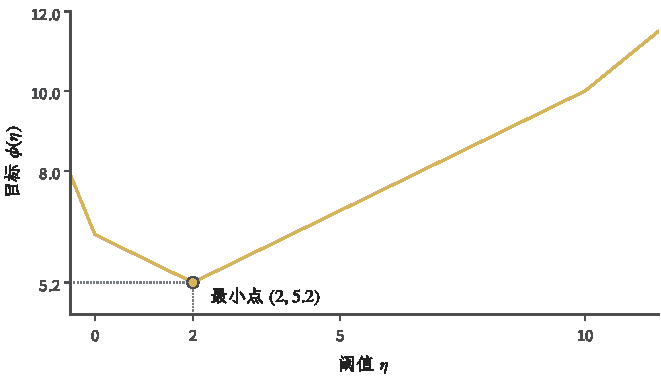
\includegraphics[width=\linewidth]{figures/math-preparation/dynamics/cvar-threshold.pdf}
  \caption{教学损失分布$P(L=0)=0.6$、$P(L=2)=0.3$、$P(L=10)=0.1$在
  $\alpha=0.75$下的阈值目标
  $\phi(\eta)=\eta+4\mathbb E[(L-\eta)_+]$。
  暖黄色折线的最小点为$(2,5.2)$；阈值$2$是VaR，最小目标值$5.2$是CVaR。
  二者位于不同坐标轴，不能把“最优阈值”当作“尾部平均损失”。}
  \label{fig:decision-cvar-threshold}
\end{figure}

\subsection{风险包络与CVaR对偶}
CVaR还有一个对鲁棒决策有用的表达。设\(L\in L^1(P)\)，则
\begin{equation}
  \operatorname{CVaR}_{\alpha}(L)
  =
  \sup_{\zeta}
  \left\{
    \mathbb{E}_P[\zeta L]:
    0\leq\zeta\leq\frac{1}{1-\alpha},\
    \mathbb{E}_P[\zeta]=1
  \right\}.
  \label{eq:decision-cvar-risk-envelope}
\end{equation}
\(\zeta\)是相对于原分布的密度比。上界
\(1/(1-\alpha)\)允许对坏结果加权，却不允许把全部质量压到任意小于
\(1-\alpha\)的事件上。

先看有限分布。对结果\(i\)及原概率\(p_i\)，令
\(q_i=p_i\zeta_i\)。右侧成为线性规划
\[
  \max_{\bm q}\sum_iq_iL_i
  \quad\text{s.t.}\quad
  0\leq q_i\leq\frac{p_i}{1-\alpha},
  \quad\sum_iq_i=1.
\]
最优解从最大损失开始填充允许的概率质量，直到总质量为\(1\)；若最后一个损失值处
只能取部分质量，正好得到式~\eqref{eq:decision-cvar-atomic-tail}中的边界补足。
图~\ref{fig:decision-cvar-reweighting}沿用$L\in\{0,2,10\}$与$\alpha=0.75$的例子，
把名义概率和最坏重加权概率放在同一损失轴上。损失$10$原有质量$0.1$，
至多可以放大到$0.4$；余下$0.6$放在损失$2$，而不是继续把所有质量堆到$10$。
这使密度比上界对应到可直接核对的概率质量。

\begin{figure}[htbp]
  \centering
  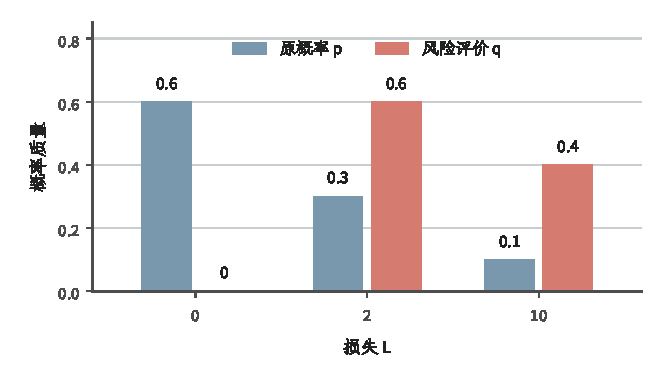
\includegraphics[width=\linewidth]{figures/math-preparation/concept-revision-dynamics/cvar-reweighting.pdf}
  \caption{教学损失$0,2,10$的名义概率为$(0.6,0.3,0.1)$。CVaR$_{0.75}$对偶中的约束
  $q_i\leq4p_i$与$\sum_iq_i=1$给出最优重加权$(0,0.6,0.4)$，
  其期望为$0.6\times2+0.4\times10=5.2$。蓝色为名义质量，红色为对偶最优质量；
  重加权只改变评价权重，不表示真实损失的发生概率已经改变。}
  \label{fig:decision-cvar-reweighting}
\end{figure}

一般表达可由相同的凸对偶关系得到。式~\eqref{eq:decision-cvar-risk-envelope}
说明CVaR是特定风险包络中的最坏期望，但这不意味着任意分布鲁棒目标都等于CVaR。

式~\eqref{eq:decision-cvar-optimization}还可直接验证CVaR的基本性质。若
\(L\leq L'\)，则对每个\(\eta\)都有
\((L-\eta)_+\leq(L'-\eta)_+\)，取下确界得到单调性。把
\(\eta'=\eta-m\)代入\(L+m\)的优化式，得到
\(\operatorname{CVaR}_\alpha(L+m)
=\operatorname{CVaR}_\alpha(L)+m\)。对\(t\geq0\)，令
\(\eta=t\bar\eta\)可得正齐次性；\(t=0\)由归一化单独成立。最后，对任意
\(\eta_1,\eta_2\)，正部函数满足
\[
  \bigl(L_1+L_2-\eta_1-\eta_2\bigr)_+
  \leq
  (L_1-\eta_1)_+
  +
  (L_2-\eta_2)_+.
\]
将这个不等式代入优化表达，并分别对\(\eta_1,\eta_2\)取下确界，得到次可加性。
正齐次性与次可加性又推出凸性。因此，对可积损失，CVaR是单调、平移等变、正齐次且
次可加的相干风险；这些性质不依赖损失分布连续。

\subsection{机会约束、最坏情形与分布鲁棒性}
若要求损失超过阈值\(b\)的概率不能太大，可以使用\term{机会约束}
（chance constraint）
\begin{equation}
  \mathbb{P}(L>b)\leq\varepsilon.
  \label{eq:decision-chance-constraint}
\end{equation}
它控制违规事件的概率，不区分违规后超出阈值多少。条件
\[
  \operatorname{CVaR}_{1-\varepsilon}(L)\leq b
\]
蕴含\(\operatorname{VaR}_{1-\varepsilon}(L)\leq b\)，进而蕴含
式~\eqref{eq:decision-chance-constraint}；这个CVaR替代通常更保守，却同时控制
尾部幅度。反方向一般不成立，因为小概率违规可以具有任意大的损失。

若模型由参数\(\theta\in\Theta\)确定，最坏情形目标
\[
  \inf_a\sup_{\theta\in\Theta}
  \mathbb{E}_{P_\theta}[\ell(a,Y)]
\]
直接比较指定模型集合中的最坏期望。\term{分布鲁棒优化}
（distributionally robust optimization, DRO）则把候选分布放入由距离、矩条件
或散度定义的集合\(\mathcal{P}\)，优化
\[
  \inf_a\sup_{Q\in\mathcal{P}}\mathbb{E}_Q[\ell(a,Y)].
\]
集合如何构造决定保证针对哪些分布；仅把“鲁棒”写进目标名称，不会自动覆盖真实分布。

仍看\(L_{\mathrm{safe}}\)与\(L_{\mathrm{tail}}\)。取事故阈值\(b=10\)和
\(\varepsilon=0.05\)，前者的违规概率为零，后者恰为\(0.05\)，所以两者都满足
机会约束；但二者的\(\operatorname{CVaR}_{0.95}\)分别为\(1\)和\(20\)。若尾部
方案中损失\(20\)的概率并非已知，而只知道\(p\in[0.02,0.08]\)，则其最坏期望为
\(\max_p20p=1.6\)，而机会约束在整个模型集合上并不成立，因为\(p=0.08>0.05\)。
逐路径最坏损失仍是\(20\)。同一有限损失表由此产生了尾部平均、违规概率、最坏期望
和逐路径上界四个不同数值。

在有限样本空间中，若\(\mathcal{P}\)是概率单纯形内的非空闭集，内层期望关于概率
向量线性，紧致性保证最坏分布达到最大值。若集合排除了某些结果，保证也只覆盖其共同
支持；若集合由估计距离球构造，“真实分布落在球内”还需要另行给出抽样置信保证。
交换\(\inf_a\)与\(\sup_Q\)或把内层最大值改写成对偶问题，则还需要凸性、紧致性、
连续性或相应约束资格，不能从有限最大值的存在自动推出。

风险准则、模型扰动与安全约束改变的是三个不同对象。CVaR改变同一损失分布的汇总方式，
最坏模型改变允许的数据生成分布，机会约束限制特定事件概率。它们可以组合，但组合前
必须明确内外层优化次序。下面先回到期望准则，建立行动会改变未来状态时的基准递推。

\section{选择影响未来状态的序贯策略}
\label{sec:decision-dynamic-programming}

静态风险准则评价一个随机后果，却尚未说明当前行动如何改变未来可选后果。
本节先以期望累计损失或奖励为基准，用状态和转移核表达这种影响，
再从条件期望的塔式性质得到Bellman递推。上节的分位数或CVaR不能直接代替递推中的期望；
它们能否跨时间组合，将在条件风险部分单独判断。

\subsection{历史策略与Markov决策过程}
考虑有限时域\(t=0,\ldots,H\)。状态\(S_t\)属于有限集合\(\mathcal{S}\)，
在状态\(s\)可选行动属于非空有限集合\(\mathcal{A}(s)\)。记时刻\(t\)采取行动前的
历史为
\[
  H_t=(S_0,A_0,\ldots,S_t).
\]
采取行动\(a\)后，付出阶段成本\(c_t(s,a)\)，下一状态按转移概率
\[
  P_t(s'\mid s,a)
  =
  \mathbb{P}(S_{t+1}=s'\mid S_t=s,A_t=a)
\]
生成，末端再付出\(c_H(S_H)\)。更具体地，MDP的Markov条件要求，对任一末状态为
\(s\)的历史\(h_t\)，后续转移核满足
\[
  \mathbb{P}(S_{t+1}=s'\mid H_t=h_t,A_t=a)
  =
  P_t(s'\mid s,a).
\]
\begin{definition}[有限Markov决策过程与策略]
\label{def:decision-finite-mdp-policy}
上述有限状态集、各状态的非空有限行动集、初始分布、转移概率、阶段及终端成本
组成有限时域
\term{Markov决策过程}（Markov decision process, MDP）。
一般策略可以根据全部历史随机选择行动，
\(\pi_t(a\mid H_t)\)。若只依赖当前状态，就称为Markov策略；若选择确定行动，
写成\(a=\pi_t(s)\)。
\end{definition}
这里的\(S_t\)承担前章状态\(\bm{x}_t\)的角色，\(A_t\)承担输入
\(\bm{u}_t\)的角色；区别在于本章先使用有限状态与有限行动，并以转移概率取代线性状态
方程。状态必须保留预测未来成本与转移所需的信息。若真实过程还依赖
未记录历史，直接把观测称为“状态”并不会使Markov性质成立\scite{math-puterman1994mdp}

对末状态为\(s\)的一段历史\(h_t\)，一般策略的继续成本应定义为
\begin{equation}
  J_t^\pi(h_t)
  =
  \mathbb{E}_{h_t}^\pi\left[
    \sum_{k=t}^{H-1}c_k(S_k,A_k)+c_H(S_H)
  \right].
  \label{eq:decision-finite-policy-value}
\end{equation}
这里的\(\mathbb{E}_{h_t}^\pi\)表示固定已有历史\(h_t\)，再由策略与转移核生成后续
过程；即使该历史在某个初始分布下概率为零，这个继续过程仍有定义。若\(\pi\)为
Markov策略，Markov条件使\(J_t^\pi(h_t)\)只依赖末状态\(s\)，此时把它记作
\(V_t^\pi(s)\)，并由条件期望得到
\begin{equation}
  V_t^\pi(s)
  =
  \sum_a\pi_t(a\mid s)
  \left[
    c_t(s,a)
    +
    \sum_{s'}P_t(s'\mid s,a)V_{t+1}^\pi(s')
  \right],
  \label{eq:decision-policy-bellman}
\end{equation}
边界条件为\(V_H^\pi(s)=c_H(s)\)。当前成本与未来价值在同一条件期望中相加，
塔式性质负责把后续随机性压缩成\(V_{t+1}^\pi\)。

\subsection{有限时域Bellman递推与策略比较}
由末端向前定义候选最优成本
\begin{align}
  V_H^\star(s)
  &=
  c_H(s),
  \label{eq:decision-finite-bellman-terminal}\\
  V_t^\star(s)
  &=
  \min_{a\in\mathcal{A}(s)}
  \left\{
    c_t(s,a)
    +
    \sum_{s'}P_t(s'\mid s,a)V_{t+1}^\star(s')
  \right\}.
  \label{eq:decision-finite-bellman}
\end{align}

\begin{theorem}[有限时域最优性原理]
\label{thm:decision-finite-horizon-optimality}
在上述有限MDP中，式~\eqref{eq:decision-finite-bellman}给出的
\(V_t^\star(s)\)满足：对每个末状态为\(s\)的历史\(h_t\)，
\[
  V_t^\star(s)=\inf_\pi J_t^\pi(h_t),
\]
其中下确界遍历所有允许的历史依赖随机继续策略。每个时刻和状态选择
式~\eqref{eq:decision-finite-bellman}中任一最小行动，得到的确定性Markov策略最优，
因此有限状态行动下该下确界可以达到。
\end{theorem}

\begin{proof}
证明采用逆向归纳。时刻\(H\)没有行动，结论由
式~\eqref{eq:decision-finite-bellman-terminal}成立。假设对每段末状态为\(s'\)的
历史\(h_{t+1}\)，\(V_{t+1}^\star(s')\)已经等于从该历史继续的最小成本。固定时刻
\(t\)的一段历史\(h_t\)，其末状态为\(s\)。任何策略在该历史下先产生一个行动分布。
给定行动\(a\)和下一状态\(s'\)后，归纳假设说明后续条件期望成本至少为
\(V_{t+1}^\star(s')\)。Markov条件保证下一状态分布为\(P_t(\cdot\mid s,a)\)，
因此该策略从\(h_t\)开始的成本至少为
\[
  \sum_a\pi_t(a\mid h_t)
  \left[
    c_t(s,a)+
    \sum_{s'}P_t(s'\mid s,a)V_{t+1}^\star(s')
  \right].
\]
右侧是各行动括号项的凸组合，不小于其中最小值，也就是
\(V_t^\star(s)\)。

反过来，在当前状态选择达到最小值的行动，并在下一时刻采用归纳假设给出的最优
Markov策略，每一步不等式都取等号，所以能够达到\(V_t^\star(s)\)。由
\(t=H-1,\ldots,0\)归纳，结论成立。
\end{proof}

这个证明同时解释了Markov策略为何足够：在已知模型和期望总成本目标下，历史对未来的
作用已经由当前状态概括。若状态遗漏信息、目标依赖整段轨迹的其他统计量，或策略还受
跨历史预算约束，必须扩充状态或重新证明这一结论。

\begin{example}[两阶段路线选择]
\label{ex:decision-two-stage-route}
初始状态\(s_0\)有“稳妥”和“捷径”两个行动，当前成本都为零。稳妥行动确定进入末端
损失\(2\)的状态；捷径以概率\(0.8\)进入损失\(0\)的状态，以概率\(0.2\)进入
损失\(6\)的状态。末端价值就是末端损失，因此
\[
  Q_0(s_0,\text{稳妥})=2,
  \qquad
  Q_0(s_0,\text{捷径})=0.8\times0+0.2\times6=1.2.
\]
期望成本准则选择捷径。这里没有声称捷径在每条路径上更好；Bellman递推比较的是给定
状态和行动后的条件期望。
\end{example}

同一个路线问题也可以比较不同评价对象，见表~\ref{tab:decision-route-risk-criteria}。
期望递推选捷径，只回答平均损失最小；若要求大损失发生的概率不超过给定预算，任务
就增加了一个不同的约束，必须重新求解。风险偏好是模型的一部分，不能在算完期望最优
以后再把它解释为任意意义下的“最稳妥”。

\begin{table}[htbp]
  \centering
  \begin{tabular}{lcc}
    \toprule
    损失评价 & 稳妥 & 捷径\\
    \midrule
    $\mathbb E[L]$ & $2$ & $1.2$\\
    $P(L>3)$ & $0$ & $0.2$\\
    $\operatorname{VaR}_{0.9}(L)$ & $2$ & $6$\\
    $\operatorname{CVaR}_{0.9}(L)$ & $2$ & $6$\\
    \bottomrule
  \end{tabular}
  \caption{两阶段教学路线在固定分布下的不同指标。捷径以概率$0.8$取损失$0$、
  以概率$0.2$取损失$6$；此处VaR和CVaR同为$6$，是因为最坏$10\%$完全落在
  损失$6$的原子中，不能推广为二者一般相等。}
  \label{tab:decision-route-risk-criteria}
\end{table}

\subsection{折扣Bellman算子与固定点}
现在令转移核\(P\)和有界阶段成本\(c\)不随时间改变，并取折扣因子
\(\gamma\in[0,1)\)。这里的\(\pi\)可以是任意历史依赖随机策略，其价值为
\begin{equation}
  V^\pi(s)
  =
  \mathbb{E}^\pi\left[
    \sum_{t=0}^{\infty}\gamma^t c(S_t,A_t)
    \,\middle|\,S_0=s
  \right].
  \label{eq:decision-discounted-value}
\end{equation}
若\(|c(s,a)|\leq C\)，几何级数保证
\(|V^\pi(s)|\leq C/(1-\gamma)\)。

在有界函数空间上定义Bellman最优算子
\begin{equation}
  (TV)(s)
  =
  \min_{a\in\mathcal{A}(s)}
  \left\{
    c(s,a)+
    \gamma\sum_{s'}P(s'\mid s,a)V(s')
  \right\}.
  \label{eq:decision-discounted-bellman-operator}
\end{equation}
对两组实数\((u_a)\)与\((v_a)\)，有
\[
  \left|\min_a u_a-\min_a v_a\right|
  \leq\max_a|u_a-v_a|.
\]
再利用转移概率非负且和为\(1\)，得到
\begin{align}
  |(TV)(s)-(TW)(s)|
  &\leq
  \gamma\max_a
  \left|
    \sum_{s'}P(s'\mid s,a)
    \bigl(V(s')-W(s')\bigr)
  \right|
  \notag\\
  &\leq
  \gamma\lVert V-W\rVert_\infty.
  \label{eq:decision-bellman-contraction-pointwise}
\end{align}
对\(s\)取最大值得
\begin{equation}
  \lVert TV-TW\rVert_\infty
  \leq
  \gamma\lVert V-W\rVert_\infty.
  \label{eq:decision-bellman-contraction}
\end{equation}

有限状态上的有界函数空间在上确界范数下完备。由第
\ref{thm:analysis-banach-fixed-point}号定理，\(T\)有唯一不动点
\(V^\star\)，价值迭代\(V^{(k+1)}=TV^{(k)}\)从任意有界初值收敛，并满足
\begin{equation}
  \lVert V^{(k)}-V^\star\rVert_\infty
  \leq
  \gamma^k
  \lVert V^{(0)}-V^\star\rVert_\infty.
  \label{eq:decision-value-iteration-error}
\end{equation}
在每个状态选择达到
\(TV^\star=V^\star\)的行动，可得到确定性平稳贪心策略。

为补上最后一步，记该贪心策略为\(\pi^\star\)，并令
\[
  (T_{\pi^\star}V)(s)
  =
  c(s,\pi^\star(s))
  +
  \gamma\sum_{s'}P(s'\mid s,\pi^\star(s))V(s').
\]
与前面的证明相同，\(T_{\pi^\star}\)也是\(\gamma\)压缩，其唯一固定点正是
\(V^{\pi^\star}\)。贪心选择又使
\(T_{\pi^\star}V^\star=TV^\star=V^\star\)，所以固定点唯一性给出
\(V^{\pi^\star}=V^\star\)。这说明Bellman固定点不仅存在，而且确实由一个平稳
确定性策略达到。

还需把这个固定点与所有其他允许策略比较。由
\(V^\star=TV^\star\)，对每个状态行动对都有Bellman不等式
\[
  V^\star(s)
  \leq
  c(s,a)+\gamma\sum_{s'}P(s'\mid s,a)V^\star(s').
\]
沿任意历史依赖随机策略\(\pi\)实际选择的行动逐步条件化，并迭代\(n\)步，得到
\begin{equation}
  V^\star(s)
  \leq
  \mathbb{E}_{s}^{\pi}\left[
    \sum_{t=0}^{n-1}\gamma^t c(S_t,A_t)
    +\gamma^nV^\star(S_n)
  \right].
  \label{eq:decision-discounted-all-policy-comparison}
\end{equation}
\(V^\star\)有界，所以余项的绝对值至多为
\(\gamma^n\lVert V^\star\rVert_\infty\)，随\(n\to\infty\)趋于零；有界成本又保证
折扣成本级数可积。令\(n\to\infty\)便得到
\(V^\star(s)\leq V^\pi(s)\)。结合
\(V^{\pi^\star}=V^\star\)，贪心策略对全部允许的历史依赖随机策略最优。

\(\gamma<1\)同时保证总成本有限并产生严格压缩。若令\(\gamma=1\)，算子通常只能
非扩张，累计成本也可能发散。长期平均成本
\[
  \limsup_{T\to\infty}
  \frac1T
  \mathbb{E}^\pi\left[\sum_{t=0}^{T-1}c(S_t,A_t)\right]
\]
需要平稳性、可达类或单链等额外条件，并常以平均成本\(g\)和相对价值\(h\)满足
\[
  g+h(s)
  =
  \min_a
  \left\{
    c(s,a)+\sum_{s'}P(s'\mid s,a)h(s')
  \right\}.
\]
\(h\)加常数后仍是解，所以不能沿用折扣问题的唯一固定点结论。

有限状态行动使取最小值、可测性和策略选取都较直接。连续状态或行动下，通常还要要求
转移核可测、成本具有适当的下半连续性、可行动作对应非空且具有紧致性或其他强制性，
并用可测选择定理把逐状态最小行动拼成策略。部分可观测时，真实状态不能直接作为策略
输入；只有在滤波信念能概括历史对未来的影响时，才能把信念分布作为新的Markov状态。
这些条件缺失时，形式上的\(\inf\)仍可写出，却未必有达到它的可实施策略。

\subsection{Bellman不等式与占用流量对偶}
有限折扣MDP还能写成线性规划。给定初始分布\(\rho\)，考虑价值端原问题
\begin{equation}
  \begin{aligned}
    \max_{V}\quad&
      (1-\gamma)\sum_s\rho(s)V(s)\\
    \text{s.t.}\quad&
      V(s)
      \leq
      c(s,a)+
      \gamma\sum_{s'}P(s'\mid s,a)V(s'),
      \quad s\in\mathcal{S},\
      a\in\mathcal{A}(s).
  \end{aligned}
  \label{eq:decision-value-lp}
\end{equation}
任一可行\(V\)满足\(V\leq TV\)。反复应用单调的\(T\)，并令迭代收敛到
\(V^\star\)，得到\(V\leq V^\star\)。而\(V^\star=TV^\star\)本身可行，
所以它达到原问题最优值。

为每条Bellman不等式引入乘子\(d(s,a)\geq0\)。拉格朗日函数为
\begin{align*}
  \mathcal{L}(V,d)
  ={}&
  (1-\gamma)\sum_s\rho(s)V(s)\\
  &-
  \sum_{s,a}d(s,a)
  \left[
    V(s)-c(s,a)
    -\gamma\sum_{s'}P(s'\mid s,a)V(s')
  \right].
\end{align*}
收集每个\(V(s)\)的系数。若要使
\(\sup_V\mathcal{L}(V,d)\)有限，必须满足
\begin{equation}
  \sum_a d(s,a)
  =
  (1-\gamma)\rho(s)
  +
  \gamma
  \sum_{\bar s,\bar a}
  P(s\mid\bar s,\bar a)d(\bar s,\bar a),
  \quad s\in\mathcal{S}.
  \label{eq:decision-discounted-flow-conservation}
\end{equation}
此时所有价值系数消失，只剩
\(\sum_{s,a}d(s,a)c(s,a)\)。因此对偶问题为
\begin{equation}
  \begin{aligned}
    \min_{d}\quad&
      \sum_{s,a}d(s,a)c(s,a)\\
    \text{s.t.}\quad&
      \text{式~\eqref{eq:decision-discounted-flow-conservation}},\\
    & d(s,a)\geq0.
  \end{aligned}
  \label{eq:decision-occupancy-lp}
\end{equation}
定理~\ref{thm:opt-lp-strong-duality}保证两个有限LP的最优值相等。

式~\eqref{eq:decision-discounted-flow-conservation}不是抽象代数条件。
\begin{definition}[归一化折扣占用度量]
\label{def:decision-discounted-occupancy}
给定初始分布$\rho$、折扣$0\leq\gamma<1$和策略\(\pi\)，定义归一化折扣
\term{占用度量}（occupancy measure）
\begin{equation}
  d_\pi(s,a)
  =
  (1-\gamma)
  \mathbb{E}_{S_0\sim\rho}^{\pi}
  \left[
    \sum_{t=0}^{\infty}
    \gamma^t
    \mathbb{I}\{S_t=s,A_t=a\}
  \right].
  \label{eq:decision-discounted-occupancy}
\end{equation}
\end{definition}
它把不同时刻访问同一状态行动对的概率相加，近时刻权重大，远时刻权重小。
乘上$1-\gamma$后总质量为$1$；这是一种访问分布，通常不同于Markov链的平稳分布。
把到达状态\(s\)的流量按初始注入和前一步转移分开，正好得到
式~\eqref{eq:decision-discounted-flow-conservation}。逐项写出便是
\begin{align*}
  \sum_a d_\pi(s,a)
  &=
  (1-\gamma)\sum_{t=0}^{\infty}
  \gamma^t\mathbb{P}^{\pi}(S_t=s)\\
  &=
  (1-\gamma)\rho(s)
  +
  \gamma(1-\gamma)
  \sum_{t=0}^{\infty}\gamma^t
  \sum_{\bar s,\bar a}
  \mathbb{P}^{\pi}(S_t=\bar s,A_t=\bar a)
  P(s\mid\bar s,\bar a)\\
  &=
  (1-\gamma)\rho(s)
  +
  \gamma\sum_{\bar s,\bar a}
  P(s\mid\bar s,\bar a)d_\pi(\bar s,\bar a).
\end{align*}
由第一行到第二行时分离\(t=0\)，把其余项的索引前移，再用全概率公式展开下一状态。
对流量方程的状态\(s\)求和，并利用转移概率和为\(1\)，可得
\[
  \sum_{s,a}d_\pi(s,a)=1.
\]
目标值则满足
\begin{equation}
  \sum_{s,a}d_\pi(s,a)c(s,a)
  =
  (1-\gamma)
  \mathbb{E}_{S_0\sim\rho}^{\pi}
  \left[
    \sum_{t=0}^{\infty}\gamma^t c(S_t,A_t)
  \right].
  \label{eq:decision-occupancy-cost}
\end{equation}

反过来，给定任一可行\(d\)，令
\[
  \pi_d(a\mid s)
  =
  \frac{d(s,a)}{\sum_{\bar a}d(s,\bar a)}
\]
用于分母为正的状态；零占用状态上的行动可以任意指定。记
\(x_d(s)=\sum_a d(s,a)\)，并把\(x_d(s)\)与\(\rho(s)\)按状态排列为列向量
\(\bm{x}_d\)与\(\bm{\rho}\)。再令
\(P_{\pi_d}(s'\mid s)=\sum_a\pi_d(a\mid s)P(s'\mid s,a)\)，代入
\(\pi_d\)后，流量方程变成
\[
  \bm{x}_d
  =
  (1-\gamma)\bm{\rho}
  +
  \gamma\bm{P}_{\pi_d}^{\top}\bm{x}_d.
\]
因为\(\gamma<1\)，矩阵
\(\bm{I}-\gamma\bm{P}_{\pi_d}^{\top}\)可由Neumann级数求逆，所以这个固定策略的
折扣状态流量方程只有一个解。策略\(\pi_d\)实际产生的状态占用也满足同一方程，因而
等于\(\bm{x}_d\)，再由
\(d(s,a)=x_d(s)\pi_d(a\mid s)\)恢复同一个状态行动占用度量。由此，价值LP在找满足
所有行动下界的最大价值，流量LP在找可实现的最小成本访问分布。

互补松弛进一步给出
\[
  d^\star(s,a)>0
  \quad\Longrightarrow\quad
  V^\star(s)
  =
  c(s,a)+\gamma\sum_{s'}P(s'\mid s,a)V^\star(s').
\]
最优占用为正的行动必须在对应状态达到Bellman最小值。若采用未乘
\(1-\gamma\)的占用量，流量方程的初始项变为\(\rho\)，总质量变为
\(1/(1-\gamma)\)；两种约定都可使用，但目标与约束必须同步归一化。

上述LP推导依赖有限状态行动、有界成本与\(\gamma<1\)。连续状态下，占用对象是测度，
价值约束是函数不等式；强对偶还需要可测选择、紧致性和适当闭性条件，不能仅把有限求和
替换成积分便宣称结论仍成立。

\section{评价观测能否改善后续行动}
\label{sec:decision-value-of-information}

动态规划在模型和当前信息给定时选择行动。若还可以先观测再行动，
新的问题是观测将怎样改变后续最优决策，以及这项改善是否值得查询成本。
信息价值沿用Bayes风险比较，探索再把获得信息与即时收益放到同一时间过程；
减少熵只在特定目标下代表决策改善。

\subsection{信息价值与观测后决策}
设未知环境参数为\(\Theta\)，当前信息为\(\mathcal{G}\)，相应信念为
\(b(\mathrm{d}\theta)=\mathbb{P}(\Theta\in\mathrm{d}\theta\mid\mathcal{G})\)。
为把重点放在信息如何改变行动，本小节假设行动集合有限，并且各行动的损失可测且可积。
一般行动空间中，下面的点态下确界还须可测，并且需要存在可测的最优或
\(\varepsilon\)-最优选择，才能对应观察后可实施的规则。
若立即选择行动\(a\)，Bayes风险为
\[
  \mathcal{R}(b)
  =
  \inf_a
  \mathbb{E}_{\theta\sim b}[\ell(a,\theta)].
\]
现在可以先观察信号\(Z\)，其条件分布由核
\(K(\mathrm{d}z\mid\theta)\)给出。观察\(Z=z\)后，信念按Bayes规则更新为
\(b_z\)，再选择适合该后验的行动。
\begin{definition}[期望样本信息价值]
\label{def:decision-expected-sample-information-value}
在上述有限行动、可积损失和给定信号核的条件下，信号的\term{期望样本信息价值}
（expected value of sample information, EVSI）定义为
\begin{equation}
  \operatorname{EVSI}(Z\mid b)
  =
  \mathcal{R}(b)
  -
  \mathbb{E}_{Z\mid b}[\mathcal{R}(b_Z)].
  \label{eq:decision-evsi}
\end{equation}
\end{definition}
这是“无信号时的最小风险”减去“看到信号后再行动的平均最小风险”。

EVSI非负。证明不需要熵或互信息，只需注意观察后总可以忽略\(Z\)，继续采用原来的
行动。若无信号风险的下确界由\(a^\star\)达到，则对每个\(z\)，
\[
  \mathcal{R}(b_z)
  \leq
  \mathbb{E}[\ell(a^\star,\Theta)\mid Z=z,\mathcal{G}].
\]
再对\(Z\)取期望并使用塔式性质，得到
\[
  \mathbb{E}_{Z\mid b}[\mathcal{R}(b_Z)]
  \leq
  \mathbb{E}[\ell(a^\star,\Theta)\mid\mathcal{G}]
  =
  \mathcal{R}(b).
\]
在一般行动空间中，若最优行动不达到但存在可测的
\(\varepsilon\)-最优选择，可改取风险不超过
\(\mathcal{R}(b)+\varepsilon\)的行动。相同推导给出观察后平均风险不超过
\(\mathcal{R}(b)+\varepsilon\)，再令\(\varepsilon\downarrow0\)，仍得到EVSI非负。
若取得信号要付成本\(k\)，应比较净价值
\(\operatorname{EVSI}-k\)。免费信息不会降低最优价值，不表示任何有成本的观测都值得
获取。

若能够直接知道\(\Theta\)，得到\term{完全信息价值}
\begin{equation}
  \operatorname{EVPI}(b)
  =
  \inf_a\mathbb{E}_{b}[\ell(a,\Theta)]
  -
  \mathbb{E}_{b}\left[\inf_a\ell(a,\Theta)\right].
  \label{eq:decision-evpi}
\end{equation}
任意样本信号都是\(\Theta\)的随机加工，决策者在知道\(\Theta\)后可以模拟该信号，
所以\(\operatorname{EVSI}\leq\operatorname{EVPI}\)。等号只在信号已经保留当前
决策所需的全部信息时成立。

\begin{example}[辨别信号与无关信号]
\label{ex:decision-informative-and-irrelevant-signals}
沿用二分类决策，设当前阳性概率为\(0.3\)，假阳性损失为\(1\)，假阴性损失为
\(9\)。不观察新信号时，预测阳性的风险为\(0.7\)，预测阴性的风险为\(2.7\)，
故\(\mathcal{R}(b)=0.7\)。若免费信号\(Z_{\mathrm{perf}}\)完全揭示类别，观察后
总能选对，平均风险降为零，因而
\(\operatorname{EVSI}(Z_{\mathrm{perf}}\mid b)=0.7\)。

另取一个与类别独立的公平硬币信号\(Z_{\mathrm{coin}}\)。无论看到哪一面，后验阳性
概率仍为\(0.3\)，最优行动和风险都不变，所以
\(\operatorname{EVSI}(Z_{\mathrm{coin}}\mid b)=0\)。若取得完全信号的成本为
\(0.8\)，其净价值反而为\(-0.1\)。可辨别性、任务价值和扣除成本后的净收益是三个
不同判断。
\end{example}

\subsection{信息量与决策价值的区别}
互信息衡量观察\(Z\)后关于\(\Theta\)的不确定性平均减少多少，信息价值衡量最优
决策损失减少多少。一个信号可以精确揭示与当前行动无关的参数，互信息很大而EVSI为零；
另一个二元信号只在临界阈值附近略微改变信念，却可能翻转高代价行动，EVSI很大。
因此，主动获取信息时必须说明优化的是预测精度、熵减少还是决策价值。

当损失为对数评分且行动本身是预测分布时，信息增益与期望对数损失改善会形成直接联系。
对一般分类代价、资源分配或控制损失，这种等价不再成立。使用熵作为查询代理时，需要
证明它与任务损失之间的关系，不能只因二者都随信息变化便混用。

\subsection{两臂选择中的探索收益}
考虑两轮选择。已知臂每次成功概率为\(0.6\)。未知臂的成功概率
\(\Theta\)只可能是\(0.3\)或\(0.9\)，先验概率各为\(1/2\)。当前未知臂的后验
均值也是\(0.6\)，所以若只看本轮期望收益，两臂并列。

若第一轮选择未知臂，成功的边缘概率为\(0.6\)。观察成功后，
\[
  \mathbb{P}(\Theta=0.9\mid\text{成功})
  =
  \frac{0.9\times0.5}
       {0.9\times0.5+0.3\times0.5}
  =0.75,
\]
下一轮未知臂的后验成功概率为
\(0.75\times0.9+0.25\times0.3=0.75\)。若第一轮失败，
\[
  \mathbb{P}(\Theta=0.9\mid\text{失败})
  =
  \frac{0.1\times0.5}
       {0.1\times0.5+0.7\times0.5}
  =0.125,
\]
未知臂的后验成功概率降为\(0.375\)，下一轮改选已知臂。
因此“先试未知臂，再按结果选择”的两轮期望收益为
\begin{equation}
  0.6+
  0.6\times0.75+
  0.4\times0.6
  =
  1.29.
  \label{eq:decision-two-arm-information-value}
\end{equation}
始终选择已知臂的期望收益为\(1.2\)。多出的\(0.09\)来自第一轮观测改变了第二轮
行动，而不是来自未知臂当前均值更高。

这个例子把\term{探索}（exploration）的核心作用写得很小：某个行动既产生即时结果，
也产生影响后续选择的信息。若只剩一轮，信息没有后续使用机会，两臂又回到并列。若
试验成本上升或先验差异缩小，探索价值也会改变。完整的多臂和强化学习算法还要处理
未知参数估计、长时域规划和计算问题，本节只建立信息进入决策的数学位置。

上述更新假设两轮共享同一个不变参数\(\Theta\)，并且每轮只观察所选臂的结果；
未选臂的反事实结果不可见。若每轮同时观察所有臂，信息结构会改变；若成功概率随时间
漂移而仍按固定\(\Theta\)更新，后验和探索收益的计算都不再对应真实过程。

\subsection{自适应反馈与统计证据}
选择最不确定的样本、反复试验某个行动或在区间足够窄时停止，都会让数据取得规则依赖
过去观测。信息价值说明为何要这样选择，却不自动保证选择后的估计仍然可靠。若希望报告
置信区间或识别最优行动，需要回到
第~\ref{sec:stoch-martingales-stopping-sequential-concentration}节的停时条件和
第~\ref{sec:stoch-self-normalized-adaptive-design}节的可预测设计，核对当前查询是否在
当前噪声揭晓前确定，以及保证是否对全部查看时刻同时成立。

遗憾则使用另一比较口径。令\(Y_t\)为第\(t\)轮观察到的随机奖励，并定义给定环境参数
\(\theta\)时的平均奖励函数。记\(\mathcal{H}_{t-1}\)为第\(t\)轮行动前可用的信息，
要求\(A_t\)在\(Y_t\)揭晓前依据这些信息选定，并假设
\[
  \mathbb{E}\left[
    Y_t
    \,\middle|\,
    \mathcal{H}_{t-1},A_t=a,\Theta=\theta
  \right]
  =
  \mu(a,\theta)
  \quad\text{几乎处处}.
\]
这个条件要求给定环境参数、历史和本轮行动后，奖励均值只由
\((a,\theta)\)决定，使当前奖励噪声在给定本轮行动后仍具有正确的条件均值；自适应选择本身
仍会改变各行动的访问次数和数据的联合分布。同时假设该均值不随
轮次改变。若第\(t\)轮选择\(A_t\)，并取
\[
  a^\star(\theta)
  \in
  \argmax_a\mu(a,\theta),
\]
则以平均奖励比较的累计伪遗憾为
\[
  \operatorname{Reg}_T(\theta)
  =
  \sum_{t=1}^{T}
  \left[
    \mu(a^\star(\theta),\theta)-\mu(A_t,\theta)
  \right].
\]
它在相同环境参数下，把算法所选行动的平均奖励与始终选择最优行动的平均奖励比较。
若算法或\(\Theta\)也是随机的，还可再对
\(\operatorname{Reg}_T(\Theta)\)取期望。直接用实现奖励之差定义的随机遗憾还包含奖励
噪声，不能与上述平均奖励差混为一谈。EVSI衡量一项信息在当前决策问题中的期望价值。
二者相关，却不能用一次信息增益直接替代长期遗憾证明。

\section{让风险评价与逐时获得的信息相容}
\label{sec:decision-dynamic-risk-time-consistency}

本节回到尾部与鲁棒要求，把静态风险准则放进逐时获得信息的决策。
关键不只是风险值能否计算，而是今天认可的计划在明天条件化之后是否仍按同一规则评价。
条件风险映射与嵌套递推规定这种规则，矩形结构则说明最坏模型能否按局部选择拼接。

\subsection{静态CVaR与条件偏好反转}
期望能够递推，是因为塔式性质把未来条件期望再平均回当前期望。若在初始时刻对整段累计
损失一次性计算CVaR，这项性质通常不再成立。下面的两阶段教学例子展示缺口。

初始时以相同概率进入节点\(N\)与节点\(B\)。节点\(N\)的损失固定为\(2\)；
在\(B\)中可以选择固定方案\(F\)或随机方案\(R\)：
\[
  L_F=3.5,
  \qquad
  L_R=
  \begin{cases}
    0,&\text{条件概率 }1/2,\\
    4,&\text{条件概率 }1/2.
  \end{cases}
\]
若初始时承诺在\(B\)选择\(F\)，总损失以概率\(1/2\)取\(2\)，以概率
\(1/2\)取\(3.5\)，所以最坏一半的平均为
\[
  \operatorname{CVaR}_{0.5}(L^{F})=3.5.
\]
若承诺选择\(R\)，无条件损失分别以概率\(1/4,1/2,1/4\)取\(0,2,4\)。
最坏一半的概率质量由全部损失\(4\)和一半的损失\(2\)组成，故
\[
  \operatorname{CVaR}_{0.5}(L^{R})
  =
  \frac{(1/4)\times4+(1/4)\times2}{1/2}
  =3.
\]
初始静态CVaR因此严格偏好承诺\(R\)。

但真正到达\(B\)以后，条件分布已经改变。此时
\[
  \operatorname{CVaR}_{0.5}(L_F\mid B)=3.5,
  \qquad
  \operatorname{CVaR}_{0.5}(L_R\mid B)=4,
\]
决策者会改选\(F\)。初始评价时，节点\(N\)的损失\(2\)占用了静态尾部的一部分；
到达\(B\)后，节点\(N\)已经排除，尾部质量只在\(B\)的条件分布中重新分配。偏好
反转来自条件化改变了排序，不是CVaR计算错误，也不表示所有风险准则都会出现同样
冲突。普通期望仍由塔式法则保持递推。

表~\ref{tab:decision-static-conditional-nested}固定同一两阶段分布，列出三种评价的
差异。静态目标把尾部预算分给整棵树；条件评价先排除未到达的分支；嵌套目标则要求每个
下一节点先给出自己的风险评价值。后者可以递推，却因此改变了最初评价的随机对象。

\begin{table*}[htbp]
  \centering
  \begin{tabularx}{\linewidth}{XccX}
    \toprule
    评价口径 & 承诺$F$ & 承诺$R$ & 比较依据\\
    \midrule
    初始静态$\operatorname{CVaR}_{0.5}$ & $3.5$ & $3$ & 整棵树最坏一半的终端损失\\
    到达$B$后的条件$\operatorname{CVaR}_{0.5}$ & $3.5$ & $4$ & $B$内部最坏一半的损失\\
    两层嵌套$\operatorname{CVaR}_{0.5}$ & $3.5$ & $4$ & 先评价下一节点，再评价节点风险\\
    \bottomrule
  \end{tabularx}
  \caption{同一教学例中的静态、条件和嵌套风险。节点$N$固定损失为$2$，根节点等概率
  到达$N$或$B$。前两行偏好反转；嵌套目标偏好$F$，但它评价的目标与静态总损失CVaR
  不同。第三行的递归定义将在下一小节建立。}
  \label{tab:decision-static-conditional-nested}
\end{table*}

\subsection{条件风险映射与信息适应性}
令
\[
  \mathcal{F}_0\subseteq\mathcal{F}_1\subseteq\cdots
  \subseteq\mathcal{F}_H
\]
表示随历史增长的信息。下一步风险应按当前历史分别评价，而不能允许阈值偷看未来结果。
\begin{definition}[一步条件风险映射]
\label{def:decision-conditional-risk-mapping}
在同一概率空间上，一步\term{条件风险映射}
（conditional risk mapping）
\[
  \rho_t:
  L^\infty(\mathcal{F}_{t+1})
  \longrightarrow
  L^\infty(\mathcal{F}_t)
\]
把下一时刻可知的有界随机损失，转换成当前信息下可比较的风险。映射作用于几乎处处
相等的等价类，因此输出也按几乎处处相等理解。
\end{definition}
常用的两项性质是：
\begin{align}
  Z\leq Z'
  &\Longrightarrow
  \rho_t(Z)\leq\rho_t(Z'),
  &&\text{单调性},
  \label{eq:decision-conditional-risk-monotonicity}\\
  \rho_t(Z+M)
  &=
  \rho_t(Z)+M,
  \quad M\in L^\infty(\mathcal{F}_t),
  &&\text{平移等变性}.
  \label{eq:decision-conditional-risk-translation}
\end{align}
第一项表示逐点更大的未来损失不应得到更低风险；第二项表示当前已经确定的成本可以直接
提出风险映射。通常还约定\(\rho_t(0)=0\)。条件期望
\(\rho_t(Z)=\mathbb{E}[Z\mid\mathcal{F}_t]\)满足这些性质。

条件CVaR可以写成
\begin{equation}
  \operatorname{CVaR}_{\alpha,t}(Z)
  =
  \operatorname*{ess\,inf}_{\eta\in
    L^\infty(\mathcal{F}_t)}
  \left\{
    \eta+
    \frac{1}{1-\alpha}
    \mathbb{E}[(Z-\eta)_+\mid\mathcal{F}_t]
  \right\}.
  \label{eq:decision-conditional-cvar}
\end{equation}
这里阈值\(\eta\)可以依赖当前历史，却不能依赖尚未观察的下一步结果。
本质下确界忽略当前概率为零的历史差异。有限概率树上，它等价于在每个当前节点分别
应用式~\eqref{eq:decision-cvar-optimization}。

\subsection{嵌套动态风险与时间一致性}
\begin{definition}[嵌套动态风险]
\label{def:decision-nested-dynamic-risk}
给定一步条件风险映射$(\rho_t)$，令\(C_t\in L^\infty(\mathcal{F}_t)\)表示时刻\(t\)已经知道的有界阶段损失。
从后向前定义
\begin{align}
  \mathcal{R}_{H}(C_H)
  &=
  C_H,\\
  \mathcal{R}_{t}(C_t,\ldots,C_H)
  &=
  C_t+
  \rho_t\bigl(
    \mathcal{R}_{t+1}(C_{t+1},\ldots,C_H)
  \bigr).
  \label{eq:decision-nested-dynamic-risk}
\end{align}
这称为\term{嵌套动态风险}（nested dynamic risk）。
\end{definition}
当前评价先接受下一时刻对
剩余损失的评价，再用当前条件风险汇总各下一状态。比较两份未来计划时，还需要固定
相同的当前损失，否则当前评价的差异可能来自已经付出的成本。
\begin{definition}[递归意义下的时间一致性]
\label{def:decision-time-consistency}
动态风险族$(\mathcal R_t)$称为具有\term{时间一致性}（time consistency），如果
对每个$t=0,\ldots,H-1$、任意两组从$t+1$开始的有界适应损失，以及同一当前损失$C_t$，只要
$\mathcal R_{t+1}(C_{t+1:H})\leq\mathcal R_{t+1}(C'_{t+1:H})$几乎处处成立，就有
$\mathcal R_t(C_t,C_{t+1:H})\leq\mathcal R_t(C_t,C'_{t+1:H})$几乎处处成立。
\end{definition}
这要求下一时刻每个可能历史中的排序被当前评价保留。若每个$\rho_t$单调，
上述嵌套结构便满足这一性质，下面直接核对这一步。
若某项阶段损失\(\widetilde C_{t+1}\)要到下一时刻才揭晓，它属于
\(L^\infty(\mathcal{F}_{t+1})\)。若用\(\widetilde{\mathcal{R}}_t\)表示这种口径下
从时刻\(t\)看到的剩余风险，相应的一步应写成
\[
  \widetilde{\mathcal{R}}_t
  =
  \rho_t\bigl(
    \widetilde C_{t+1}+\widetilde{\mathcal{R}}_{t+1}
  \bigr),
\]
不能把\(\widetilde C_{t+1}\)作为当前已知量放在\(\rho_t\)之外。

形式地，若
\[
  \mathcal{R}_{t+1}(C_{t+1:H})
  \leq
  \mathcal{R}_{t+1}(C'_{t+1:H})
  \quad\text{几乎处处},
\]
单调性立即给出
\[
  C_t+
  \rho_t\bigl(\mathcal{R}_{t+1}(C_{t+1:H})\bigr)
  \leq
  C_t+
  \rho_t\bigl(\mathcal{R}_{t+1}(C'_{t+1:H})\bigr).
\]
证明很短，因为时间一致性已经被递归结构编码进去。它不说明嵌套CVaR等于初始时对
总累计损失计算一次静态CVaR；前面的两节点例子恰好说明两者会给出不同目标。

在该例中，若每个节点都使用
\(\operatorname{CVaR}_{0.5}\)，节点\(B\)先把
\(F\)评价为\(3.5\)、把\(R\)评价为\(4\)，所以选择\(F\)。根节点再对
“节点\(N\)为\(2\)、节点\(B\)为\(3.5\)”计算条件CVaR，得到\(3.5\)。
嵌套目标选择\(F\)，而静态总损失CVaR选择预先承诺\(R\)。二者不是同一目标的两种
算法实现。

\subsection{风险Bellman递推}
在Markov状态已经保留条件风险所需信息时，可把一步条件风险写成依赖状态行动的映射
\(\rho_{s,a}\)。有限时域风险价值满足
\begin{align}
  V_H(s)
  &=
  c_H(s),\\
  V_t(s)
  &=
  \min_{a\in\mathcal{A}(s)}
  \left\{
    c_t(s,a)+
    \rho_{t,s,a}\bigl(V_{t+1}(S_{t+1})\bigr)
  \right\}.
  \label{eq:decision-risk-bellman-finite}
\end{align}
其中随机变量\(V_{t+1}(S_{t+1})\)的分布由
\(P_t(\cdot\mid s,a)\)给出。若\(\rho\)取条件期望，
式~\eqref{eq:decision-risk-bellman-finite}退化为普通Bellman递推；若取条件CVaR，
它计算的是逐阶段嵌套CVaR\scite{math-ruszczynski2010risk}

无限折扣情形定义
\begin{equation}
  (T_\rho V)(s)
  =
  \min_a
  \left\{
    c(s,a)+
    \gamma
    \rho_{s,a}\bigl(V(S')\bigr)
  \right\}.
  \label{eq:decision-risk-bellman-operator}
\end{equation}
假设成本有界，每个一步风险映射满足单调性、平移等变性和归一化。若
\(\lVert V-W\rVert_\infty\leq\delta\)，则逐点有
\[
  W(S')-\delta
  \leq
  V(S')
  \leq
  W(S')+\delta.
\]
单调性与平移等变性给出
\[
  \rho_{s,a}(W(S'))-\delta
  \leq
  \rho_{s,a}(V(S'))
  \leq
  \rho_{s,a}(W(S'))+\delta.
\]
因此每个一步风险映射都非扩张。这里\(V,W\)是有限状态上的实际向量，
\(\delta\)使用普通最大范数，并且不涉及零测集上的等价类。若改用一般
\(L^\infty\)空间，还须确认转移核不会读取所选代表在零测集上的任意取值，不能未经
核对便把同一证明逐字搬过去。再使用最小值差的基本不等式，
\begin{equation}
  \lVert T_\rho V-T_\rho W\rVert_\infty
  \leq
  \gamma\lVert V-W\rVert_\infty.
  \label{eq:decision-risk-bellman-contraction}
\end{equation}
当\(\gamma<1\)时，Banach定理给出唯一有界固定点和价值迭代的几何收敛。

这个压缩证明只回答算子是否有唯一固定点。要把固定点解释为所声明的动态风险最优值，
还须核对三项条件：风险目标是否确实按
式~\eqref{eq:decision-nested-dynamic-risk}递归；当前状态是否包含风险评价所需的
历史信息；允许策略类是否与Bellman逐状态选择相容。一个收敛的递推可以稳定地求解
错误目标，压缩性不会替代建模核对。

\subsection{静态CVaR的状态增广}
若目标是
\[
  \operatorname{CVaR}_{\alpha}
  \left(
    \sum_{t=0}^{H}\gamma^t C_t
  \right),
\]
不能一般在原状态上把普通期望替换成一步CVaR。由
式~\eqref{eq:decision-cvar-optimization}，可先固定阈值\(\eta\)，再最小化
\[
  \eta+
  \frac{1}{1-\alpha}
  \mathbb{E}
  \left[
    \left(
      \sum_{t=0}^{H}\gamma^tC_t-\eta
    \right)_+
  \right].
\]
正部函数依赖截至当前已经累计了多少损失以及还剩多少阈值。把累计损失或剩余阈值加入
状态后，可以对固定\(\eta\)建立动态规划，最后再优化\(\eta\)。这种状态增广保留的是
静态总损失CVaR；直接改用嵌套条件CVaR则改变了目标。

增广状态可能连续，计算规模也会增大。若阶段损失无界，还需保证正部期望有限；若策略
可以依赖累计损失，允许策略类也随状态增广而扩大。所谓“CVaR可以动态规划”必须同时
说明采用的是哪种表示、优化哪种策略，以及递推对应静态还是嵌套风险。

\subsection{风险包络与矩形结构}
无罚项的概率包络需要比单调和平移等变更强的条件。先固定一个具有\(m\)个结果的有限
空间，把一步风险写成\(\rho:\mathbb{R}^m\to\mathbb{R}\)。若\(\rho\)归一化，
并同时满足单调性、平移等变性、正齐次性和次可加性，它就是相干风险。正齐次与次可加
使\(\rho\)成为有限凸的次线性函数。定义
\[
  \mathcal{Q}
  =
  \left\{
    \bm q\in\mathbb{R}^m:
    \langle\bm q,\bm z\rangle\leq\rho(\bm z)
    \text{ 对所有 }\bm z\in\mathbb{R}^m
  \right\}.
\]
有限维次线性函数的支撑表示给出
\[
  \rho(\bm z)
  =
  \max_{\bm q\in\mathcal{Q}}
  \langle\bm q,\bm z\rangle.
\]
具体地说，\(\rho\)的凸共轭在\(\mathcal{Q}\)上为零、在其外为无穷，
Fenchel--Moreau对偶便得到上式。平移等变性应用于
\(\bm z+r\bm 1\)迫使每个\(\bm q\in\mathcal{Q}\)满足
\(\langle\bm q,\bm 1\rangle=1\)；单调性再迫使\(q_i\geq0\)。因此
\(\mathcal{Q}\)是概率单纯形中的非空闭凸集，有限维紧致性保证最大值达到。

若风险仅为归一化、单调、平移等变的凸风险，正齐次可能不成立。此时一般对偶形式为
\[
  \rho(\bm z)
  =
  \sup_{\bm q\in\Delta_m}
  \left\{
    \langle\bm q,\bm z\rangle-\beta(\bm q)
  \right\},
\]
其中\(\Delta_m=\{\bm q\in\mathbb{R}_+^m:
\langle\bm q,\bm 1\rangle=1\}\)是概率单纯形，\(\beta\)是允许取无穷值的凸罚函数；
不能无条件删去罚项并称为最坏期望。

回到Markov过程，若每个状态行动处都使用相干的一步条件风险映射，便可写成风险包络中
的最坏条件期望：
\begin{equation}
  \rho_{s,a}(V(S'))
  =
  \sup_{q\in\mathcal{Q}(s,a)}
  \sum_{s'}q(s'\mid s,a)V(s').
  \label{eq:decision-one-step-risk-envelope}
\end{equation}
条件CVaR对应对名义转移概率作有上界的密度重加权。把
式~\eqref{eq:decision-one-step-risk-envelope}代入
式~\eqref{eq:decision-risk-bellman-operator}，得到
\[
  (T_\rho V)(s)
  =
  \min_a
  \sup_{q\in\mathcal{Q}(s,a)}
  \left\{
    c(s,a)+\gamma\sum_{s'}q(s'\mid s,a)V(s')
  \right\}.
\]
它看起来像鲁棒MDP，但递推还依赖不确定集合能否按历史逐步选择。

\begin{definition}[条件分布集合的矩形性]
\label{def:decision-rectangular-uncertainty}
在有限概率树上，为每个历史行动节点给定非空的下一步条件分布集合。如果允许的
路径分布恰好包括从各节点集合中任意选取条件核并按路径相乘得到的全部分布，
就称该不确定集合具有\term{矩形性}（rectangularity）。
\end{definition}
在Markov表达中，各节点使用$\mathcal Q(s,a)$，当前选择可以依赖已发生历史，
却不受其他节点选择同一个未知参数等跨节点约束。矩形性允许把整条路径上的最坏分布拆成逐节点最坏
条件分布，风险包络才与Bellman递推相容。

若不确定性在多个时刻之间共享同一个未知参数，允许的路径分布通常是耦合的。例如一个
固定但未知的故障率必须在全程保持相同，不能在每个状态分别挑选最坏故障率。逐节点取
上确界会允许一个并不存在的对手沿历史改变参数，相当于把原集合扩张成矩形包络，结果
可能更保守，也可能定义完全不同的最坏模型问题。此时应保留共享参数的信念或把它加入
状态，而不是把非矩形集合直接塞入普通Bellman算子。

一个二次观测的有限例子可以直接检验这个差别。设$Y_1,Y_2\in\{0,1\}$在给定
未知$p\in\{0.2,0.8\}$后独立，且两次都使用同一个成功率$p$。原模型对事件
$Y_1=1,Y_2=0$赋予的概率只有$p(1-p)=0.16$。若逐节点独立选择最坏成功率，
就可在第一步取$0.8$，在已见$Y_1=1$后改取$0.2$，把该事件概率提高到$0.64$。
$0.64$不属于任何一个原来的固定参数模型；这个数值差精确说明矩形扩张增加了哪些路径分布。
若问题确实允许对手逐时改变$p$，局部递推便对应这个新模型；若$p$固定未知，
递推状态还应保留关于$p$的信念与共享约束。

动态风险的边界由此清楚起来。单调性和平移等变性给出一步非扩张，折扣产生压缩；
递归嵌套给出时间一致性，状态充分性保证当前节点拥有正确条件信息；风险包络若要解释为
逐步鲁棒选择，还需矩形结构。任一条件缺失，形式相似的递推都可能不再评价原先声明的
随机损失。

\section{本章小结}
\label{sec:decision-theory-and-dynamic-risk-summary}

概率预测只有与行动和损失结合后，才能回答应该做什么。条件风险把后验分布中的各项
结果按损失加权，Bayes规则再选择条件风险最小的行动。错误代价、拒答成本和总体预算
会改变阈值，即使概率输出完全相同也可能产生不同的合理决策；随机化只有在并列或耦合
约束下才提供额外作用。

风险准则规定怎样汇总随机损失。期望控制平均结果，方差同时计算好坏两侧的波动，VaR
给出分位切点，CVaR则通过分位点优化平均最坏尾部。离散分布的分位点可能承载正概率，
此时必须从边界原子中补足尾部质量。CVaR的风险包络说明它等价于一类受限重加权下的
最坏期望；机会约束、一般最坏模型与分布鲁棒目标仍分别控制违规概率、模型集合和分布
集合，不能仅凭“保守”二字合并。

行动影响未来状态后，策略价值由条件期望和状态转移共同决定。有限时域Bellman递推可由
逆向归纳证明，折扣Bellman算子则在有界函数的上确界范数下成为压缩。价值端的Bellman
不等式与流量端的非负占用度量构成一对线性规划；初始分布、折扣归一化和流量守恒使
对偶变量具有真实访问频率的含义。平均成本与连续状态问题需要额外条件，不能从有限折扣
结论直接外推。

信息之所以有价值，不是因为它必然减少某种抽象不确定性，而是因为观察后可以改变行动。
EVSI比较观察前后的最优Bayes风险，多臂例子中的探索收益来自当前试验改善下一轮选择。
自适应取得数据同时改变统计证据的条件，仍需序贯集中和可预测设计支持误差结论。

静态总损失CVaR可能在到达未来分支后发生偏好反转。条件风险映射按当前信息评价未来，
递归嵌套由单调性保持跨时排序，从而建立时间一致的动态风险。对单调且平移等变的一步
风险映射，折扣风险Bellman算子仍是压缩；但固定点要对应正确目标，还需状态充分、策略
类相容和正确的递归定义。静态CVaR通常需要累计损失或阈值的状态增广，风险包络的逐步
鲁棒解释还需要矩形性。下一章将在这些价值对象上加入受控动力学，推导线性二次控制、
安全反馈与连续时间最优性条件；随后的博弈论章则进一步允许其他参与者也选择策略。

\chapter{控制理论}
\label{chap:control-theory}

第~\ref{chap:dynamical-systems-and-state-estimation}章研究了输入给定以后，状态怎样演化、扰动怎样传播，以及有限观测能够提供多少状态信息。第~\ref{chap:decision-theory-and-dynamic-risk}章又为跨时刻的行动后果建立了价值递推。还缺的一步是把输入本身变成待选择的对象：系统每到一个状态，都要依据当前可用信息决定下一次作用。这样形成的
\term{反馈}（feedback）会改变后续状态，后续状态又会改变未来的反馈。

这一步不能只靠写出一个优化目标。某个不稳定方向可能根本不受输入影响，某个影响决策的状态方向也可能无法从观测辨认；即使期望成本达到最小，轨迹仍可能穿过不可接受的区域。控制理论分别询问这些问题：哪些动态模式能够被输入改变，哪些模式能够被输出识别，怎样在长期稳定的前提下优化成本，以及怎样让每条允许轨迹都留在安全集合内。

本章先在线性状态空间中建立可控、可稳定、可观测和可检测四个结构条件。它们为线性二次调节和稳态滤波说明“解为什么存在且能稳定系统”。随后，我们从有限时域价值递推完整推出Riccati递推，并将成本最优与安全集合保持分开。最后把离散时间的Bellman原理缩到一个短时间区间，得到连续时间的Hamilton--Jacobi--Bellman方程。四节讨论的是同一个受控动态的不同要求；一个要求成立，不能替代其余要求。
\section{判断输入能否改变、观测能否区分动态模式}
\label{sec:control-feedback-structure}
\subsection{开环、状态反馈与输出反馈}
考虑离散时间线性时不变系统
\begin{equation}
  \begin{aligned}
    \bm{x}_{t+1}
      &=\bm{A}\bm{x}_t+\bm{B}\bm{u}_t,\\
    \bm{y}_t
      &=\bm{C}\bm{x}_t,
  \end{aligned}
  \label{eq:control-state-space}
\end{equation}
其中$\bm{x}_t\in\mathbb{R}^{n}$是状态，$\bm{u}_t\in\mathbb{R}^{m}$是控制输入，
$\bm{y}_t\in\mathbb{R}^{p}$是观测。矩阵维度相应为
$\bm{A}\in\mathbb{R}^{n\times n}$、$\bm{B}\in\mathbb{R}^{n\times m}$和
$\bm{C}\in\mathbb{R}^{p\times n}$。这里明确令直接传递矩阵为零，因此时刻$t$先由
$\bm{x}_t$产生$\bm{y}_t$，控制器再计算$\bm{u}_t$。若保留
$\bm{y}_t=\bm{C}\bm{x}_t+\bm{D}\bm{u}_t$并允许$\bm{u}_t$依赖当前
$\bm{y}_t$，两式会形成需要另行求解适定性的代数环；另一种无环约定是只让控制使用
截至$t-1$的观测。

“用当前状态计算动作”与“用当前读数计算动作”限制了控制器能使用的信息，不能仅靠
同一个反馈增益符号将两者混用。
\begin{definition}[开环控制与反馈控制]
\label{def:control-open-loop-state-output-feedback}
对式~\eqref{eq:control-state-space}，若$\bm{u}_0,\bm{u}_1,\bm{u}_2,\ldots$事先指定，
输入不根据运行中实际出现的状态修正，就称为\term{开环控制}（open-loop control）。
若状态能够直接取得，依据当前状态选择动作的
\[
  \bm{u}_t=\kappa_t(\bm{x}_t)
\]
是状态反馈；只有观测历史可用时，
\[
  \bm{u}_t
  =
  \mu_t(\bm{y}_0,\ldots,\bm{y}_t;
  \bm{u}_0,\ldots,\bm{u}_{t-1})
\]
称为输出反馈，其中空的初始控制历史按空序列处理。
\end{definition}
由于本节采用零直接传递，
当前观测$\bm{y}_t$不含尚未计算的$\bm{u}_t$。写出依赖真实状态的公式，不等于
传感器已经提供了该状态。

反馈把原系统与控制律合成一个新的闭环动力系统，因而还要重新检查解是否存在且唯一。离散时间递推只要每一步的反馈有定义，就能逐步生成轨迹；连续时间系统则通常要求动态与反馈满足局部Lipschitz等适定性条件。若反馈在切换面不连续，必须改用适合不连续右端的解概念，不能只凭形式上的闭环方程断言轨迹唯一。

最简单的线性状态反馈取
\begin{equation}
  \bm{u}_t=-\bm{K}\bm{x}_t,
  \qquad
  \bm{x}_{t+1}
  =(\bm{A}-\bm{B}\bm{K})\bm{x}_t.
  \label{eq:control-state-feedback}
\end{equation}
因此闭环离散系统渐近稳定，当且仅当$\bm{A}-\bm{B}\bm{K}$的全部特征值都严格位于单位圆内。这里的负号只是约定；若写$\bm{u}_t=\bm{F}\bm{x}_t$，对应闭环矩阵就是$\bm{A}+\bm{B}\bm{F}$。

反馈能否把不稳定特征值移入单位圆，取决于输入是否真正作用到相应状态方向。这不是优化算法精度问题，而是矩阵对$(\bm{A},\bm{B})$本身的结构性质。
\subsection{可达子空间与可控性}
把式~\eqref{eq:control-state-space}连续展开$N$步，可得
\begin{equation}
  \bm{x}_N
  =
  \bm{A}^{N}\bm{x}_0
  +
  \sum_{t=0}^{N-1}
  \bm{A}^{N-1-t}\bm{B}\bm{u}_t.
  \label{eq:control-reachability-unrolling}
\end{equation}
固定初态后，终态中能被控制改变的部分属于
\[
  \operatorname{span}
  \{\bm{B},\bm{A}\bm{B},\ldots,
    \bm{A}^{N-1}\bm{B}\}
\]
的列空间。这些列依次表示一次输入经过零步、一步直至$N-1$步传播后能够产生的状态方向。
\begin{definition}[可控性]
\label{def:control-controllability}
若对任意初态$\bm{x}_0$和任意目标状态$\bm{x}_{\mathrm f}$，都存在有限时刻$N$及输入序列$\bm{u}_0,\ldots,\bm{u}_{N-1}$，使$\bm{x}_N=\bm{x}_{\mathrm f}$，则称$(\bm{A},\bm{B})$可控。
\end{definition}
对线性时不变系统，“从任意初态到任意终态”与“从零到任意终态”等价：式~\eqref{eq:control-reachability-unrolling}对输入线性，自由响应$\bm{A}^N\bm{x}_0$可以移到目标一侧。这两种性质都蕴含任意初态可以在有限时间驱动到零，但反向一般不成立。后一种较弱的性质称为\term{零可控性}。例如，标量系统$A=0,B=0$会使任意初态在一步后自然变为零，却无法从零到达非零状态；当$\bm{A}$可逆时，零可控性才可反推出这里定义的可控性。
\begin{theorem}[Kalman可控性秩判据]
\label{thm:control-controllability-rank}
定义可控性矩阵
\begin{equation}
  \mathcal{C}(\bm{A},\bm{B})
  =
  \begin{bmatrix}
    \bm{B}&\bm{A}\bm{B}&\cdots&\bm{A}^{n-1}\bm{B}
  \end{bmatrix}.
  \label{eq:control-controllability-matrix}
\end{equation}
系统$(\bm{A},\bm{B})$可控，当且仅当
\[
  \operatorname{rank}\mathcal{C}(\bm{A},\bm{B})=n.
\]
\end{theorem}
\begin{proof}
先取$N=n$。把输入按逆时间顺序堆成向量，式~\eqref{eq:control-reachability-unrolling}中的受控部分可以写成
\[
  \mathcal{C}(\bm{A},\bm{B})
  \begin{bmatrix}
    \bm{u}_{n-1}\\
    \bm{u}_{n-2}\\
    \vdots\\
    \bm{u}_0
  \end{bmatrix}.
\]
若可控性矩阵满行秩，它的列张成$\mathbb{R}^n$，所以对任意$\bm{x}_{\mathrm f}-\bm{A}^n\bm{x}_0$都能找到输入，系统可控。

反过来，若该矩阵秩小于$n$，其列空间是$\mathbb{R}^n$的真子空间。Cayley--Hamilton定理说明$\bm{A}^n$可写成$\bm{I},\bm{A},\ldots,\bm{A}^{n-1}$的线性组合；继续乘$\bm{A}$可知，每个$\bm{A}^k\bm{B}$（$k\geq n$）仍落在$\mathcal{C}(\bm{A},\bm{B})$的列空间中。延长时域不会增加新的可达方向，因而从零出发无法到达该列空间外的状态，系统不可控。
\end{proof}
最小的算例是标量积分系统$x_{t+1}=x_t+u_t$。给定$x_0$与目标$x_{\mathrm f}$，一步取$u_0=x_{\mathrm f}-x_0$即可到达，因而其可控性矩阵$[1]$满秩。若改成二维系统
\[
  \bm{A}=
  \begin{bmatrix}
    1&1\\
    0&1
  \end{bmatrix},
  \qquad
  \bm{B}=
  \begin{bmatrix}
    0\\1
  \end{bmatrix},
\]
则当前输入先改变第二个坐标，经过一次状态传播后再影响第一个坐标。此时
\[
  \begin{bmatrix}\bm{B}&\bm{A}\bm{B}\end{bmatrix}
  =
  \begin{bmatrix}
    0&1\\
    1&1
  \end{bmatrix}
\]
满秩，两个坐标都可达。相反，若$\bm{A}=\bm{I}$而$\bm{B}=(1,0)^{\top}$，输入无论作用多久都只能改变第一个坐标；延长时域不会补出缺失方向。

图~\ref{fig:control-reachable-directions}保留刚才的二维系统，并为教学示意暂时加入
$|u_0|,|u_1|\leq1$。从零出发，一步只能沿$\bm B$移动，两步终态为
$\bm x_2=\bm A\bm B u_0+\bm B u_1=(u_0,u_0+u_1)^\top$。
有界输入形成一个平行四边形；解除幅值限制后，两个独立方向张成整个平面，
这才对应秩判据中的无约束可控性。图中可达区域的面积与能到达任意状态是不同说法。
\begin{figure}[htbp]
  \centering
  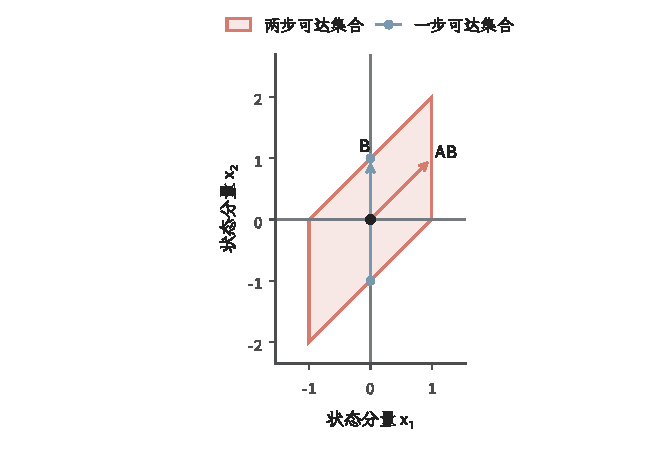
\includegraphics[width=\linewidth]{figures/math-preparation/concept-revision-dynamics/reachable-directions.pdf}
  \caption{教学系统$\bm A=\left[\begin{smallmatrix}1&1\\0&1\end{smallmatrix}\right]$、
  $\bm B=(0,1)^\top$与零初态。蓝色线段为$|u_0|\leq1$时的一步可达集合，
  红色区域为$|u_0|,|u_1|\leq1$时的两步可达集合；箭头标出$\bm B$与$\bm A\bm B$。
  输入先改变第二个坐标，经一次状态传播后获得新的方向。输入幅值界只服务于有限区域的绘图，
  不属于定理~\ref{thm:control-controllability-rank}的无约束假设。}
  \label{fig:control-reachable-directions}
\end{figure}

连续时间线性系统$\dot{\bm{x}}=\bm{A}\bm{x}+\bm{B}\bm{u}$具有相同问题，但输入通过积分累积。由状态转移公式，
\[
  \bm{x}(T)
  =
  e^{\bm{A}T}\bm{x}_0
  +
  \int_0^T e^{\bm{A}(T-s)}\bm{B}\bm{u}(s)\,\mathrm{d}s.
\]
定义时域$T>0$上的\term{可控Gram矩阵}
\begin{equation}
  \bm{W}_{\mathrm c}(T)
  =
  \int_0^T
  e^{\bm{A}s}\bm{B}\bm{B}^{\top}e^{\bm{A}^{\top}s}
  \,\mathrm{d}s.
  \label{eq:control-controllability-gramian}
\end{equation}
连续线性系统在$[0,T]$上可控，当且仅当$\bm{W}_{\mathrm c}(T)\succ\bm{0}$。事实上，对任意$\bm{q}\in\mathbb{R}^n$，
\[
  \bm{q}^{\top}\bm{W}_{\mathrm c}(T)\bm{q}
  =
  \int_0^T
  \lVert
    \bm{B}^{\top}e^{\bm{A}^{\top}s}\bm{q}
  \rVert_2^2\,\mathrm{d}s.
\]
若Gram矩阵奇异，就存在非零$\bm{q}$使被积函数恒为零，该方向与所有受控终态增量正交，因而不可达。若Gram矩阵正定，则对所需增量$\bm{d}=\bm{x}_{\mathrm f}-e^{\bm{A}T}\bm{x}_0$取
\[
  \bm{u}(s)
  =
  \bm{B}^{\top}e^{\bm{A}^{\top}(T-s)}
  \bm{W}_{\mathrm c}(T)^{-1}\bm{d},
\]
代入状态转移公式便得到终态增量$\bm{d}$。这个Gram判据依赖线性时不变结构；一般非线性系统即使在一点把Jacobian矩阵代入，也只能得到局部线性化信息，不能据此推出全局可控。

秩判据回答“整个状态空间是否可达”，但有时我们只需判断某个动态模式是否受控。在复数域上考察$\bm{A}$的左特征向量会得到更直接的判据。
\begin{theorem}[Popov--Belevitch--Hautus（PBH）可控性判据]
\label{thm:control-pbh-controllability}
矩阵对$(\bm{A},\bm{B})$可控，当且仅当对$\bm{A}$的每个复特征值$\lambda$都有
\begin{equation}
  \operatorname{rank}
  \begin{bmatrix}
    \lambda\bm{I}-\bm{A}&\bm{B}
  \end{bmatrix}
  =n.
  \label{eq:control-pbh-controllability}
\end{equation}
等价地，不存在非零左特征向量$\bm{q}^{\ast}$满足$\bm{q}^{\ast}\bm{A}=\lambda\bm{q}^{\ast}$且$\bm{q}^{\ast}\bm{B}=\bm{0}$。
\end{theorem}
\begin{proof}
若存在这样的$\bm{q}$，则对每个$k\geq0$，
\[
  \bm{q}^{\ast}\bm{A}^k\bm{B}
  =
  \lambda^k\bm{q}^{\ast}\bm{B}
  =\bm{0}.
\]
所以可控性矩阵的每一列都位于$\bm{q}^{\ast}$的零空间，不可能满行秩。

反向可用$\bm{A}$不变子空间说明。若可控性矩阵不满秩，它的列空间$\mathcal{R}$是一个真子空间，并且$\bm{A}\mathcal{R}\subseteq\mathcal{R}$。于是正交补$\mathcal{R}^{\perp}$在$\bm{A}^{\ast}$下不变。复数域上的非零有限维不变子空间包含$\bm{A}^{\ast}$的一个特征向量$\bm{q}$。它正交于$\mathcal{R}$，特别有$\bm{q}^{\ast}\bm{B}=\bm{0}$，从而式~\eqref{eq:control-pbh-controllability}在相应特征值处不满秩。
\end{proof}
\subsection{可控分解与可稳定性}
完全可控时，极点配置定理允许通过状态反馈配置闭环特征值；稳定系统并不总需要这么强的条件。若某个不可控模式本身已经衰减，就没有必要通过输入移动它。
\begin{definition}[可稳定性]
\label{def:control-stabilizability}
若存在矩阵$\bm{K}$，使$\bm{A}-\bm{B}\bm{K}$的全部特征值严格位于单位圆内，则称离散时间矩阵对$(\bm{A},\bm{B})$可稳定。
\end{definition}

这个结论可以由Kalman可控分解看清。令$\mathcal{R}$为可控性矩阵的列空间，并选择以$\mathcal{R}$的一组基为前若干列的可逆矩阵$\bm{T}$。由于$\bm{A}\mathcal{R}\subseteq\mathcal{R}$且$\operatorname{col}(\bm{B})\subseteq\mathcal{R}$，在坐标$\bm{z}=\bm{T}^{-1}\bm{x}$下有
\[
  \bm{T}^{-1}\bm{A}\bm{T}
  =
  \begin{bmatrix}
    \bm{A}_{\mathrm c}&\bm{A}_{12}\\
    \bm{0}&\bm{A}_{\mathrm{uc}}
  \end{bmatrix},
  \qquad
  \bm{T}^{-1}\bm{B}
  =
  \begin{bmatrix}
    \bm{B}_{\mathrm c}\\
    \bm{0}
  \end{bmatrix},
\]
其中$(\bm{A}_{\mathrm c},\bm{B}_{\mathrm c})$可控。把$\bm{K}\bm{T}$分块写成
$[\bm{K}_{\mathrm c}\ \bm{K}_{\mathrm{uc}}]$后，闭环矩阵在同一坐标下变为
\[
  \begin{bmatrix}
    \bm{A}_{\mathrm c}-\bm{B}_{\mathrm c}\bm{K}_{\mathrm c}
    &
    \bm{A}_{12}-\bm{B}_{\mathrm c}\bm{K}_{\mathrm{uc}}\\
    \bm{0}&\bm{A}_{\mathrm{uc}}
  \end{bmatrix}.
\]
反馈可以通过$\bm{K}_{\mathrm c}$配置可控块的特征值，却不能改变不可控块$\bm{A}_{\mathrm{uc}}$的特征值。因此，存在稳定化反馈当且仅当不可控块本身稳定。PBH矩阵在特征值$\lambda$处不满秩，恰好表示$\lambda$属于这个不可控块；所以只需排除不稳定和临界的不可控模式：
\begin{equation}
  \operatorname{rank}
  \begin{bmatrix}
    \lambda\bm{I}-\bm{A}&\bm{B}
  \end{bmatrix}
  =n
  \quad
  \text{对每个满足 }|\lambda|\geq1
  \text{ 的 }\lambda\in\sigma(\bm{A}).
  \label{eq:control-pbh-stabilizability}
\end{equation}
可控必然推出可稳定，反向并不成立。这个差别在无限时域调节中很重要：已经稳定但无法控制的模式可以留在原处，无法控制的不稳定模式却会使任何线性反馈都失败。
\begin{example}[不可控但可稳定的系统]
\label{ex:control-stabilizable-not-controllable}
令
\[
  \bm{A}=
  \begin{bmatrix}
    1.2&0\\
    0&0.5
  \end{bmatrix},
  \qquad
  \bm{B}=
  \begin{bmatrix}
    1\\0
  \end{bmatrix}.
\]
可控性矩阵
\[
  \begin{bmatrix}\bm{B}&\bm{A}\bm{B}\end{bmatrix}
  =
  \begin{bmatrix}
    1&1.2\\
    0&0
  \end{bmatrix}
\]
只有秩$1$，第二个模式不可控。但它的特征值为$0.5$，已经位于单位圆内。取$\bm{K}=(1,0)$，闭环特征值变成$0.2$和$0.5$，所以该系统可稳定。若交换$\bm{B}$的两个分量，使输入只能作用到$0.5$模式，则$1.2$模式不可控，系统便不可稳定。
\end{example}
\subsection{可观测性、可检测性与观测器}
控制器若只能看见输出，就要先问不同初态能否由输出序列区分。暂取输入为零；已知输入对输出的贡献可以计算并扣除，不改变以下结构判据。连续观察$n$个时刻得到
\begin{equation}
  \begin{bmatrix}
    \bm{y}_0\\
    \bm{y}_1\\
    \vdots\\
    \bm{y}_{n-1}
  \end{bmatrix}
  =
  \underbrace{
  \begin{bmatrix}
    \bm{C}\\
    \bm{C}\bm{A}\\
    \vdots\\
    \bm{C}\bm{A}^{n-1}
  \end{bmatrix}}_{\mathcal{O}(\bm{C},\bm{A})}
  \bm{x}_0.
  \label{eq:control-observability-matrix}
\end{equation}
\begin{definition}[可观测性与可检测性]
\label{def:control-observability-detectability}
若式~\eqref{eq:control-observability-matrix}中的观测矩阵$\mathcal{O}(\bm{C},\bm{A})$满列秩，则称$(\bm{C},\bm{A})$可观测。若存在矩阵$\bm{L}$使$\bm{A}-\bm{L}\bm{C}$的全部特征值严格位于单位圆内，则称$(\bm{C},\bm{A})$可检测。
\end{definition}
可观测意味着有限输出序列能够唯一确定任意初态。这个秩条件也可以从“输出能否区分两个初态”直接证明。若$\mathcal{O}$满列秩，则线性方程~\eqref{eq:control-observability-matrix}至多有一个$\bm{x}_0$，所以输出序列唯一确定初态。反之，若$\mathcal{O}$不满列秩，就存在非零$\bm{v}$满足$\mathcal{O}\bm{v}=\bm{0}$；初态$\bm{x}_0$与$\bm{x}_0+\bm{v}$在前$n$个时刻产生相同输出。Cayley--Hamilton定理又使所有$\bm{C}\bm{A}^k\bm{v}$（$k\geq n$）都是前$n$项的线性组合，所以继续观察也无法区分这两个初态。

可检测只要求所有无法从输出辨认的模式自行稳定；不可见但会衰减的状态不会阻止估计误差趋于零。二者的PBH判据分别为
\begin{align}
  \operatorname{rank}
  \begin{bmatrix}
    \lambda\bm{I}-\bm{A}\\
    \bm{C}
  \end{bmatrix}
  &=n
  &&\text{对每个 }\lambda\in\sigma(\bm{A}),
  \label{eq:control-pbh-observability}\\
  \operatorname{rank}
  \begin{bmatrix}
    \lambda\bm{I}-\bm{A}\\
    \bm{C}
  \end{bmatrix}
  &=n
  &&\text{对每个 }|\lambda|\geq1.
  \label{eq:control-pbh-detectability}
\end{align}
把$\bm{A}$换成$\bm{A}^{\top}$、把$\bm{B}$换成$\bm{C}^{\top}$，可控性矩阵的转置正是观测矩阵。对偶矩阵对$(\bm{A}^{\top},\bm{C}^{\top})$应用上述Kalman分解，可知反馈无法移动它的不可控块，而该块正对应原系统的不可观测模式。又因为
\[
  \bm{A}^{\top}-\bm{C}^{\top}\bm{L}^{\top}
  =
  (\bm{A}-\bm{L}\bm{C})^{\top},
\]
两侧具有相同特征值，所以式~\eqref{eq:control-pbh-detectability}既是必要条件也是充分条件：不可观测块稳定时，可以配置其余观测器误差模式；不可观测块含危险特征值时，任何$\bm{L}$都无法消除它。这就是可控与可观测、可稳定与可检测之间的线性代数对偶。

连续时间版本只改变“危险模式”的稳定区域。对$\dot{\bm{x}}=\bm{A}\bm{x}+\bm{B}\bm{u}$，可稳定性要求
\[
  \operatorname{rank}
  \begin{bmatrix}
    \lambda\bm{I}-\bm{A}&\bm{B}
  \end{bmatrix}
  =n
  \quad
  \text{对每个满足 }\operatorname{Re}\lambda\geq0
  \text{ 的 }\lambda\in\sigma(\bm{A});
\]
对输出$\bm{y}=\bm{C}\bm{x}$，可检测性要求相应的纵向PBH矩阵满列秩。分解与对偶论证和离散情形相同，只把单位圆外替换为闭右半平面。该接口将在连续时间Riccati稳态条件中使用。

继续使用示例~\ref{ex:control-stabilizable-not-controllable}中的$\bm{A}$。若$\bm{C}=(1,0)$，不稳定的$1.2$模式可以观测，稳定的$0.5$模式不可观测；系统不可观测但可检测。若改成$\bm{C}=(0,1)$，输出完全看不到$1.2$模式，估计误差中的该分量会增长，系统不可检测。
表~\ref{tab:control-structural-properties}把输入与输出两侧放在同一尺度下比较。
“完整恢复或到达”要求每个方向都可处理；“只求长期稳定”允许遗漏那些本来就会衰减的
方向。前者更强，却未必是当前控制目标必需的条件。

\begin{table*}[htbp]
  \centering
  \begin{tabularx}{\linewidth}{lXXX}
    \toprule
    性质 & 所比较的对象 & 哪些方向必须处理 & 二维例的判断\\
    \midrule
    可控 & 输入与终态 & 全部状态方向 & 否，输入无法改变第二坐标\\
    可稳定 & 反馈与闭环谱 & 不稳定及临界模式 & 是，$1.2$模式受控\\
    可观测 & 初态与输出序列 & 全部状态方向 & 否，输出不含第二坐标\\
    可检测 & 观测器与误差谱 & 不稳定及临界模式 & 是，$1.2$模式可见\\
    \bottomrule
  \end{tabularx}
  \caption{线性系统的四种结构条件。二维教学例固定
  $\bm A=\operatorname{diag}(1.2,0.5)$、$\bm B=(1,0)^\top$、$\bm C=(1,0)$。
  第二模式虽不可控且不可观测，却自行衰减；若将其特征值改为$1.1$，可稳定与可检测
  两项也会失败。连续时间用特征值实部代替模长判断危险模式。}
  \label{tab:control-structural-properties}
  \label{tab:control-structural-comparison}
\end{table*}

\subsection{观测器与状态反馈的谱分离}
状态不可直接取得时，可以用\term{Luenberger观测器}根据模型、输入和输出更新估计：
\begin{equation}
  \widehat{\bm{x}}_{t+1}
  =
  \bm{A}\widehat{\bm{x}}_t+\bm{B}\bm{u}_t
  +
  \bm{L}\bigl(
    \bm{y}_t-\bm{C}\widehat{\bm{x}}_t
  \bigr).
  \label{eq:control-luenberger-observer}
\end{equation}
令估计误差$\bm{e}_t=\bm{x}_t-\widehat{\bm{x}}_t$，直接相减得到
\[
  \bm{e}_{t+1}
  =
  (\bm{A}-\bm{L}\bm{C})\bm{e}_t.
\]
因此可检测性正是选择$\bm{L}$使误差渐近消失所需的结构条件。

将状态反馈改为$\bm{u}_t=-\bm{K}\widehat{\bm{x}}_t$后，用$\bm{x}_t$和$\bm{e}_t$作为联合状态可得
\begin{equation}
  \begin{bmatrix}
    \bm{x}_{t+1}\\
    \bm{e}_{t+1}
  \end{bmatrix}
  =
  \begin{bmatrix}
    \bm{A}-\bm{B}\bm{K}&\bm{B}\bm{K}\\
    \bm{0}&\bm{A}-\bm{L}\bm{C}
  \end{bmatrix}
  \begin{bmatrix}
    \bm{x}_t\\
    \bm{e}_t
  \end{bmatrix}.
  \label{eq:control-separation-block}
\end{equation}
该矩阵是分块上三角矩阵，其特征值是两个对角块特征值的并集。因此，只要$(\bm{A},\bm{B})$可稳定且$(\bm{C},\bm{A})$可检测，就能分别选择$\bm{K}$和$\bm{L}$，使整个确定性线性闭环稳定。这一
\term{分离原理}并不表示估计与控制在所有问题中都互不影响；非线性、约束、模型误差
或风险敏感目标可能破坏这种简单分离。
表~\ref{tab:control-structural-properties}中的输入和输出两侧由转置联系。
完全结构条件覆盖全部状态方向，稳定化结构条件只排除危险的遗漏方向；
后面的Riccati条件会分别调用这两侧的较弱条件，而不会要求每个系统都完全可控且完全可观测。

\section{在二次成本下设计反馈与估计器}
\label{sec:control-lqr-riccati}

结构分析已经说明哪些方向可受控、哪些方向可观测。现在在这些条件下给定二次成本，
寻找具体反馈。有限时域的Bellman递推保持价值函数的二次形式，因而导出Riccati递推；
无限时域还需稳定化条件，不能把有限时域可配方直接当作稳态解存在的证明。
\subsection{二次价值函数与有限时域Riccati递推}
结构条件说明稳定反馈是否可能存在，却没有选择具体反馈。现在为状态偏离和控制用力分别计价。
\begin{definition}[有限时域线性二次调节]
\label{def:control-finite-horizon-lqr}
考虑有限时域随机线性系统
\begin{equation}
  \bm{x}_{t+1}
  =
  \bm{A}\bm{x}_t+\bm{B}\bm{u}_t+\bm{w}_t,
  \qquad t=0,\ldots,T-1,
  \label{eq:control-lqr-dynamics}
\end{equation}
以及成本
\begin{equation}
  J
  =
  \mathbb{E}\left[
    \bm{x}_T^{\top}\bm{Q}_T\bm{x}_T
    +
    \sum_{t=0}^{T-1}
    \left(
      \bm{x}_t^{\top}\bm{Q}\bm{x}_t
      +
      \bm{u}_t^{\top}\bm{R}\bm{u}_t
    \right)
  \right].
  \label{eq:control-lqr-cost}
\end{equation}
这里$\bm{Q},\bm{Q}_T\in\mathbb{R}^{n\times n}$且$\bm{Q},\bm{Q}_T\succeq\bm{0}$，$\bm{R}\in\mathbb{R}^{m\times m}$且$\bm{R}\succ\bm{0}$。半正定状态代价允许某些状态方向不直接计价；正定控制代价保证每一步关于$\bm{u}_t$的二次目标严格凸。

在可用信息规定的非预见控制策略中最小化$J$，称为\term{线性二次调节}
（linear-quadratic regulation, LQR）。
\end{definition}

先假设状态完全可见，且$\bm{w}_t$相互独立、均值为零、协方差为$\bm{\Sigma}_{\mathrm{w}}$，并与当前状态和动作独立。令$\mathcal{F}_t=\sigma(\bm{x}_0,\ldots,\bm{x}_t)$表示截至时刻$t$可用的状态信息，并用$\Pi_t$表示从$t$到$T-1$的允许反馈策略；对任意$\pi\in\Pi_t$，控制$\bm{u}_{\tau}$必须对$\mathcal{F}_{\tau}$可测，不能预先利用未来噪声。定义从时刻$t$起的最优剩余成本
\[
  V_t(\bm{x})
  =
  \inf_{\pi\in\Pi_t}
  \mathbb{E}\left[
    \bm{x}_T^{\top}\bm{Q}_T\bm{x}_T
    +
    \sum_{\tau=t}^{T-1}
    \bigl(
      \bm{x}_{\tau}^{\top}\bm{Q}\bm{x}_{\tau}
      +
      \bm{u}_{\tau}^{\top}\bm{R}\bm{u}_{\tau}
    \bigr)
    \,\middle|\,\bm{x}_t=\bm{x}
  \right].
\]
这里的下确界对适应当前状态信息的策略取，而不是对事先固定的开环控制序列取。终端价值为
$V_T(\bm{x})=\bm{x}^{\top}\bm{Q}_T\bm{x}$\scite{math-anderson2007lqr}
第~\ref{chap:decision-theory-and-dynamic-risk}章的Bellman原理给出
\begin{equation}
  V_t(\bm{x})
  =
  \min_{\bm{u}}
  \left\{
    \bm{x}^{\top}\bm{Q}\bm{x}
    +
    \bm{u}^{\top}\bm{R}\bm{u}
    +
    \mathbb{E}
    \left[
      V_{t+1}(
        \bm{A}\bm{x}+\bm{B}\bm{u}+\bm{w}_t)
    \right]
  \right\}.
  \label{eq:control-lqr-bellman}
\end{equation}
\begin{theorem}[有限时域LQR与Riccati递推]
\label{thm:control-finite-horizon-lqr}
在上述条件下，最优价值具有形式
\[
  V_t(\bm{x})
  =
  \bm{x}^{\top}\bm{P}_t\bm{x}+c_t,
\]
其中$\bm{P}_T=\bm{Q}_T$、$c_T=0$。令
\begin{equation}
  \begin{aligned}
    \bm{S}_t
      &=
      \bm{R}+\bm{B}^{\top}\bm{P}_{t+1}\bm{B},\\
    \bm{K}_t
      &=
      \bm{S}_t^{-1}
      \bm{B}^{\top}\bm{P}_{t+1}\bm{A}.
  \end{aligned}
  \label{eq:control-lqr-gain}
\end{equation}
则最优控制为
\[
  \bm{u}_t^{\ast}=-\bm{K}_t\bm{x}_t,
\]
而$\bm{P}_t$满足离散Riccati递推
\begin{equation}
  \bm{P}_t
  =
  \bm{Q}
  +
  \bm{A}^{\top}\bm{P}_{t+1}\bm{A}
  -
  \bm{A}^{\top}\bm{P}_{t+1}\bm{B}
  \bm{S}_t^{-1}
  \bm{B}^{\top}\bm{P}_{t+1}\bm{A}.
  \label{eq:control-discrete-riccati-recursion}
\end{equation}
噪声只进入常数项
\begin{equation}
  c_t
  =
  c_{t+1}
  +
  \operatorname{tr}(\bm{P}_{t+1}\bm{\Sigma}_{\mathrm{w}}).
  \label{eq:control-lqr-noise-constant}
\end{equation}
\end{theorem}
\begin{proof}
采用反向归纳。终端时刻的结论由$\bm{P}_T=\bm{Q}_T,c_T=0$成立。假设$t+1$时刻价值已经具有所述形式。记
\[
  \bm{z}
  =
  \bm{A}\bm{x}+\bm{B}\bm{u}.
\]
零均值和独立性给出
\begin{align*}
  \mathbb{E}
  [V_{t+1}(\bm{z}+\bm{w}_t)]
  &=
  \mathbb{E}
  [(\bm{z}+\bm{w}_t)^{\top}
    \bm{P}_{t+1}
    (\bm{z}+\bm{w}_t)]
  +c_{t+1}\\
  &=
  \bm{z}^{\top}\bm{P}_{t+1}\bm{z}
  +
  \operatorname{tr}(\bm{P}_{t+1}\bm{\Sigma}_{\mathrm{w}})
  +c_{t+1}.
\end{align*}
交叉项的条件期望为零。将$\bm{z}$展开，并只收集与控制有关的项，Bellman目标成为
\begin{align*}
  &\bm{x}^{\top}
  (\bm{Q}+\bm{A}^{\top}\bm{P}_{t+1}\bm{A})
  \bm{x}
  +
  2\bm{u}^{\top}
  \bm{B}^{\top}\bm{P}_{t+1}\bm{A}\bm{x}\\
  &\quad+
  \bm{u}^{\top}
  (\bm{R}+\bm{B}^{\top}\bm{P}_{t+1}\bm{B})
  \bm{u}
  +
  \operatorname{tr}(\bm{P}_{t+1}\bm{\Sigma}_{\mathrm{w}})
  +c_{t+1}.
\end{align*}
因为$\bm{R}\succ\bm{0}$且$\bm{P}_{t+1}\succeq\bm{0}$，$\bm{S}_t\succ\bm{0}$。以式~\eqref{eq:control-lqr-gain}中的$\bm{K}_t$配方，
\begin{align*}
  &\bm{u}^{\top}\bm{S}_t\bm{u}
  +
  2\bm{u}^{\top}
  \bm{B}^{\top}\bm{P}_{t+1}\bm{A}\bm{x}\\
  &\quad=
  (\bm{u}+\bm{K}_t\bm{x})^{\top}
  \bm{S}_t
  (\bm{u}+\bm{K}_t\bm{x})
  -
  \bm{x}^{\top}\bm{K}_t^{\top}
  \bm{S}_t\bm{K}_t\bm{x}.
\end{align*}
第一项非负，并且仅在$\bm{u}=-\bm{K}_t\bm{x}$时为零。把剩余二次项合并，恰好得到式~\eqref{eq:control-discrete-riccati-recursion}；与状态无关的项给出式~\eqref{eq:control-lqr-noise-constant}。Riccati右端保持半正定，于是归纳可以继续到$t=0$。
\end{proof}
该证明同时解释了“二次价值族在Bellman备份下封闭”的含义：线性动态把状态与动作送入二次型，最小化动作后仍留下状态的二次型。一般非线性动态或非二次代价不具有这个闭合关系，不能仅把矩阵换成Jacobian矩阵就得到精确LQR。

噪声不改变反馈增益也有明确边界。这里用到了噪声条件均值为零、与当前决策独立，以及风险中性期望成本。若噪声均值非零，价值函数一般还需要线性项，最优控制会出现仿射偏置；若噪声分布受动作影响、与状态相关，或目标惩罚尾部风险，噪声可能直接改变反馈律。
\subsection{标量LQR的配方与反馈增益}
取无噪声标量系统
\[
  x_{t+1}=1.2x_t+u_t,
  \qquad
  Q=R=1.
\]
若下一步价值系数为$P_{t+1}$，则
\[
  S_t=1+P_{t+1},
  \qquad
  K_t=\frac{1.2P_{t+1}}{1+P_{t+1}},
\]
并且
\[
  P_t
  =
  1+1.44P_{t+1}
  -
  \frac{1.44P_{t+1}^2}{1+P_{t+1}}
  =
  1+\frac{1.44P_{t+1}}{1+P_{t+1}}.
\]
当终端代价$P_T=0$时，倒数第一步有$P_{T-1}=1$，$K_{T-1}=0$；最后一个动作之后没有状态代价，所以此时不用力。再向前一步得到$P_{T-2}=1.72$和$K_{T-2}=0.6$。时域变长后，远离终端的增益逐渐接近稳态值。
\subsection{无限时域LQR与稳定化Riccati解}
本小节切换到确定性系统，即在式~\eqref{eq:control-lqr-dynamics}中令$\bm{w}_t=\bm{0}$。对时不变、无折扣的无限时域问题，考虑总成本
\[
  J_{\infty}
  =
  \sum_{t=0}^{\infty}
  \left(
    \bm{x}_t^{\top}\bm{Q}\bm{x}_t
    +
    \bm{u}_t^{\top}\bm{R}\bm{u}_t
  \right).
\]
该级数并非对任意控制都有限；稳定化条件用于保证最优反馈下的状态和控制充分衰减。希望$\bm{P}_t$和$\bm{K}_t$不再随时间变化。将$\bm{P}_{t+1}=\bm{P}_t=\bm{P}$代入式~\eqref{eq:control-discrete-riccati-recursion}，得到
\term{离散代数Riccati方程}（discrete algebraic Riccati equation, DARE）：
\begin{equation}
  \bm{P}
  =
  \bm{Q}
  +
  \bm{A}^{\top}\bm{P}\bm{A}
  -
  \bm{A}^{\top}\bm{P}\bm{B}
  (\bm{R}+\bm{B}^{\top}\bm{P}\bm{B})^{-1}
  \bm{B}^{\top}\bm{P}\bm{A}.
  \label{eq:control-dare}
\end{equation}
一个满足代数等式的矩阵未必就是所需解。控制所需的是
\term{稳定化解}：除满足$\bm{P}\succeq\bm{0}$外，它产生的
\[
  \bm{K}
  =
  (\bm{R}+\bm{B}^{\top}\bm{P}\bm{B})^{-1}
  \bm{B}^{\top}\bm{P}\bm{A}
\]
还要使$\bm{A}-\bm{B}\bm{K}$稳定。
\begin{theorem}[无限时域LQR的稳定化解]
\label{thm:control-infinite-horizon-lqr}
设$\bm{Q}\succeq\bm{0}$、$\bm{R}\succ\bm{0}$。若$(\bm{A},\bm{B})$可稳定，且$(\bm{Q}^{1/2},\bm{A})$可检测，则式~\eqref{eq:control-dare}存在唯一的半正定稳定化解$\bm{P}$。由该解得到的线性反馈使闭环渐近稳定，并给出无限时域二次成本的最优值$V(\bm{x})=\bm{x}^{\top}\bm{P}\bm{x}$。
\end{theorem}
\begin{proof}
这里给出决定条件作用的证明主线。对终端矩阵取$\bm{P}_N=\bm{0}$，从长度$N$的有限时域问题反向递推，并记初始时刻矩阵为$\bm{P}^{(N)}$。增加一个非负阶段成本不会降低最优成本，所以
\[
  \bm{0}\preceq
  \bm{P}^{(N)}
  \preceq
  \bm{P}^{(N+1)}.
\]
可稳定性保证存在某个$\overline{\bm{K}}$使$\bm{A}-\bm{B}\overline{\bm{K}}$稳定。始终采用这一反馈所得无限时域成本有限，因此它为所有有限时域最优成本提供统一二次上界。单调且有上界的半正定矩阵序列收敛到某个$\bm{P}\succeq\bm{0}$。Riccati映射连续，取极限便得到式~\eqref{eq:control-dare}。

令$\bm{A}_{\bm{K}}=\bm{A}-\bm{B}\bm{K}$。将DARE按最优增益重写为
\begin{equation}
  \bm{P}
  -
  \bm{A}_{\bm{K}}^{\top}
  \bm{P}\bm{A}_{\bm{K}}
  =
  \bm{Q}+\bm{K}^{\top}\bm{R}\bm{K}.
  \label{eq:control-dare-lyapunov}
\end{equation}
右侧半正定。现在用可检测性排除闭环中的非衰减模式。若
$\bm{A}_{\bm K}$存在特征对
$\bm{A}_{\bm K}\bm{z}=\lambda\bm{z}$，其中
$\bm{z}\neq\bm{0}$且$|\lambda|\geq1$，在
式~\eqref{eq:control-dare-lyapunov}两侧左乘$\bm{z}^{*}$、右乘$\bm{z}$，得到
\[
  (1-|\lambda|^2)\bm{z}^{*}\bm{P}\bm{z}
  =
  \lVert\bm{Q}^{1/2}\bm{z}\rVert_2^2
  +
  \lVert\bm{R}^{1/2}\bm{K}\bm{z}\rVert_2^2.
\]
左侧非正而右侧非负，所以两侧只能同时为零。特别地，
$\bm{Q}^{1/2}\bm{z}=\bm{0}$且$\bm{K}\bm{z}=\bm{0}$。于是
\[
  \bm{A}\bm{z}
  =
  (\bm{A}_{\bm K}+\bm{B}\bm{K})\bm{z}
  =
  \lambda\bm{z},
\]
这给出了$(\bm{Q}^{1/2},\bm{A})$无法检测的危险特征向量，与假设矛盾。因此
$\bm{A}_{\bm K}$的全部特征值严格位于单位圆内，极限解确实是稳定化解。

记$\bm{S}=\bm{R}+\bm{B}^{\top}\bm{P}\bm{B}$。对任意控制序列，把Bellman配方恒等式
沿前$N$步求和，得到
\[
  \sum_{t=0}^{N-1}
  \left(
    \bm{x}_t^{\top}\bm{Q}\bm{x}_t
    +
    \bm{u}_t^{\top}\bm{R}\bm{u}_t
  \right)
  +
  \bm{x}_N^{\top}\bm{P}\bm{x}_N
  =
  \bm{x}_0^{\top}\bm{P}\bm{x}_0
  +
  \sum_{t=0}^{N-1}
  (\bm{u}_t+\bm{K}\bm{x}_t)^{\top}
  \bm{S}
  (\bm{u}_t+\bm{K}\bm{x}_t).
\]
这里不能在令$N\to\infty$时直接丢掉终端项。若某个允许控制的总成本有限，则
\[
  \bm{Q}^{1/2}\bm{x}_t\to\bm{0},
  \qquad
  \bm{u}_t\to\bm{0};
\]
第二个结论使用了$\bm{R}\succ\bm{0}$。由
$(\bm{Q}^{1/2},\bm{A})$可检测，可选$\bm{L}$使
$\bm{A}-\bm{L}\bm{Q}^{1/2}$稳定，并把状态递推写成
\[
  \bm{x}_{t+1}
  =
  (\bm{A}-\bm{L}\bm{Q}^{1/2})\bm{x}_t
  +
  \bm{B}\bm{u}_t
  +
  \bm{L}\bm{Q}^{1/2}\bm{x}_t.
\]
右侧稳定线性系统的输入趋于零，因此$\bm{x}_t\to\bm{0}$，进而
$\bm{x}_N^{\top}\bm{P}\bm{x}_N\to0$。这就是可检测性在终端项论证中的具体作用。
总成本无限的控制自然不可能优于稳定反馈。令$N\to\infty$后，任意有限成本控制的成本
等于$\bm{x}_0^{\top}\bm{P}\bm{x}_0$加上一串
\[
  (\bm{u}_t+\bm{K}\bm{x}_t)^{\top}
  (\bm{R}+\bm{B}^{\top}\bm{P}\bm{B})
  (\bm{u}_t+\bm{K}\bm{x}_t)
\]
的极限和。采用$\bm{u}_t=-\bm{K}\bm{x}_t$时这些平方项为零，闭环稳定也使终端项趋零，故该反馈达到下界并最优。同一恒等式应用于两个半正定稳定化解，可知二者都表示同一最优成本，因而相等。
\end{proof}
示例中的标量DARE为
\[
  P=1+\frac{1.44P}{1+P},
  \qquad
  P^2-1.44P-1=0.
\]
半正定解是
\[
  P=\frac{1.44+\sqrt{6.0736}}{2}\approx1.952,
  \qquad
  K=\frac{1.2P}{1+P}\approx0.794.
\]
闭环系数$1.2-K\approx0.406$，位于单位圆内。另一个代数根为负，不表示非负无限时域成本，也不是这里的稳定化解。

可检测条件中的“输出”是$\bm{Q}^{1/2}\bm{x}$，不是传感器输出$\bm{C}\bm{x}$。它要求任何不被状态成本惩罚的不稳定模式都不存在。传感器的可检测性则决定估计误差能否稳定，两种条件服务于不同对象。

一个标量反例说明为何代数解和成本最优都不足以替代“稳定化”。令$A=1.2$、$B=1$、$Q=0$、$R=1$。系统可控，却因为$Q^{1/2}=0$而无法检测不稳定模式。DARE同时有$P=0$和$P=0.44$两个半正定解：前者给出$K=0$和不稳定闭环$1.2$，后者给出稳定闭环$1.2-1.2P/(1+P)=5/6$。然而原目标只惩罚控制，取$u_t=0$便以零成本达到全局最小；稳定化解对应正控制成本，反而不是该退化目标的最优解。可检测性正是用来排除这种“不稳定状态完全免费”的情形，不能在求出某个DARE根以后省略。

无限时域切换到确定性系统也不是无关紧要的简化。若每一步都有非零独立加性噪声，即使闭环稳定，状态协方差通常也会收敛到非零稳态值，单步期望状态成本便不会趋于零；无折扣累计期望成本因而通常发散。此时应明确改用长期平均成本、折扣成本或有限时域目标。只有当噪声及其传播方向恰好不被成本计入等退化情形，才可能避开这一结论。
\subsection{滤波Riccati对偶与LQG分离}
第~\ref{chap:dynamical-systems-and-state-estimation}章的有限时域Kalman滤波在每一步先传播协方差，再用新观测修正。若采用预测协方差$\bm{\Pi}_t$，状态噪声协方差为$\bm{\Sigma}_{\mathrm{w}}\succeq\bm{0}$，观测噪声协方差为$\bm{\Sigma}_{\mathrm{v}}\succ\bm{0}$，稳态预测方程可写成
\begin{equation}
  \bm{\Pi}
  =
  \bm{A}\bm{\Pi}\bm{A}^{\top}
  +\bm{\Sigma}_{\mathrm{w}}
  -
  \bm{A}\bm{\Pi}\bm{C}^{\top}
  (\bm{C}\bm{\Pi}\bm{C}^{\top}+\bm{\Sigma}_{\mathrm{v}})^{-1}
  \bm{C}\bm{\Pi}\bm{A}^{\top}.
  \label{eq:control-filter-dare}
\end{equation}
这里$\bm{\Pi}$是观测$\bm{y}_t$到来之前的预测误差协方差。令
\[
  \widehat{\bm{x}}_{t|t-1}
  =
  \mathbb{E}[\bm{x}_t\mid\mathcal{Y}_{t-1}],
\]
其中$\mathcal{Y}_{t-1}$包含截至$t-1$的观测和已执行控制，并在稳态记
\[
  \bm{\Pi}
  =
  \mathbb{E}\left[
    (\bm{x}_t-\widehat{\bm{x}}_{t|t-1})
    (\bm{x}_t-\widehat{\bm{x}}_{t|t-1})^{\top}
  \right].
\]
采用观测模型$\bm{y}_t=\bm{C}\bm{x}_t+\bm{v}_t$时，与式~\eqref{eq:control-filter-dare}口径一致的合并观测更新与一步预测为
\[
  \widehat{\bm{x}}_{t+1|t}
  =
  \bm{A}\widehat{\bm{x}}_{t|t-1}
  +\bm{B}\bm{u}_t
  +\bm{L}
  \bigl(
    \bm{y}_t-\bm{C}\widehat{\bm{x}}_{t|t-1}
  \bigr),
\]
其中
\[
  \bm{L}
  =
  \bm{A}\bm{\Pi}\bm{C}^{\top}
  (\bm{C}\bm{\Pi}\bm{C}^{\top}+\bm{\Sigma}_{\mathrm{v}})^{-1}.
\]
因此齐次预测误差矩阵是$\bm{A}-\bm{L}\bm{C}$。若把
$\bm{\Pi}\bm{C}^{\top}
(\bm{C}\bm{\Pi}\bm{C}^{\top}+\bm{\Sigma}_{\mathrm{v}})^{-1}$
称为观测更新增益，则从更新后估计传播到下一时刻时还要左乘$\bm{A}$；两种增益不能在同一协方差口径下混用。

将控制DARE中的
\[
  \bm{A}\leftrightarrow\bm{A}^{\top},
  \quad
  \bm{B}\leftrightarrow\bm{C}^{\top},
  \quad
  \bm{Q}\leftrightarrow\bm{\Sigma}_{\mathrm{w}},
  \quad
  \bm{R}\leftrightarrow\bm{\Sigma}_{\mathrm{v}},
\]
便得到这一形式。控制增益用输入压低状态成本，滤波增益用观测压低估计误差协方差；公式对偶不表示两者的随机变量含义相同。

一个常用的充分条件是$(\bm{C},\bm{A})$可检测、$(\bm{A},\bm{\Sigma}_{\mathrm{w}}^{1/2})$可稳定且$\bm{\Sigma}_{\mathrm{v}}\succ\bm{0}$。在这些条件及标准独立噪声假设下，协方差递推收敛到唯一稳定化半正定解，稳态滤波增益使估计误差动态稳定。可检测性保证危险状态模式能从观测纠正；过程噪声对偶条件排除Riccati方程在不稳定方向上的退化。有限时域滤波本身不要求协方差已经收敛，稳态公式也不能在系统时变、噪声统计变化或模型严重错设时直接替代逐时递推。

滤波结果怎样进入控制，还需要一条信息接口。在线性动态、二次成本、高斯初值与独立加性高斯噪声的标准有限时域设定中，令
\[
  \widehat{\bm{x}}_t
  =
  \mathbb{E}[\bm{x}_t\mid\mathcal{Y}_t],
  \qquad
  \bm{e}_t=\bm{x}_t-\widehat{\bm{x}}_t,
\]
其中$\mathcal{Y}_t$包含截至$t$的观测和已执行控制。条件期望的投影性质给出
\[
  \mathbb{E}[\bm{e}_t\mid\mathcal{Y}_t]=\bm{0},
  \qquad
  \mathbb{E}
  [\widehat{\bm{x}}_t^{\top}\bm{Q}\bm{e}_t]=0.
\]
因此条件状态成本分解为估计均值的二次成本与误差协方差项；在该设定下，Kalman误差协方差递推又不依赖所选控制值。Bellman递推中与当前动作有关的部分遂与完全状态LQR相同，只需把真实状态换成条件均值：
\[
  \bm{u}_t^{\ast}
  =
  -\bm{K}_t\widehat{\bm{x}}_t.
\]
这就是线性二次高斯控制中的\term{分离原则}：Kalman滤波器按估计误差设计，LQR增益按行动成本设计，再通过估计均值连接。它比前文确定性观测器的谱分离多给出期望成本最优性，但依赖噪声、信息和二次目标的特殊结构；受控观测噪声、风险敏感目标、输入或状态约束都可能使估计价值依赖未来控制，从而破坏这一分离。
\section{把轨迹安全转化为可行动作约束}
\label{sec:control-safety-cbf}

成本最优并不自动保证所有状态约束成立。本节另加轨迹必须留在安全集合内的要求，
用集合边界上的可行方向建立屏障条件，再把名义控制投影到可行输入集合。
这项保证与LQR成本是两种要求：安全条件先确定允许哪些动作，优化再从中选择。
\subsection{安全集合与正向不变性}
LQR惩罚偏离和控制强度，所得反馈对给定二次目标最优。但有限代价或渐近稳定都不保证状态从未越过危险区域。一个制动系统最终回到零速度，仍可能在停止前越过边界；一个平均成本很小的随机系统，也可能存在少量不可接受轨迹。安全控制需要逐轨迹描述允许状态，并证明闭环向量场不会把状态推出该集合。

离散系统可以先用一步条件看清这一要求。设闭环映射为$\bm{x}_{t+1}=F_{\kappa}(\bm{x}_t)$，安全集合为$S$。若
\begin{equation}
  F_{\kappa}(S)\subseteq S,
  \label{eq:control-discrete-invariance}
\end{equation}
则从$\bm{x}_0\in S$出发，归纳可得$\bm{x}_1\in S$，继而$\bm{x}_2\in S$，并对每个$t\geq0$都有$\bm{x}_t\in S$。反过来，若要求$S$中的每个初态都正向不变，取任意$\bm{x}\in S$考察第一步，就必须有$F_{\kappa}(\bm{x})\in S$。因此式~\eqref{eq:control-discrete-invariance}对确定性离散闭环既充分又必要。

例如，对$x_{t+1}=x_t+u_t$取安全集合$S=[0,\infty)$。反馈$u_t=-1.5x_t$产生$x_{t+1}=-0.5x_t$，状态幅值会趋于零，却从任意$x_0>0$在第一步就越过安全边界；反馈$u_t=-0.5x_t$则产生$x_{t+1}=0.5x_t$，既渐近稳定又保持非负。原系统能够到达负半轴只说明它可达，不能说明所选闭环应该到达那里。这个例子把可达、稳定与安全分成了三个不同判断。

连续时间不能只检查采样时刻的一步映射，因为轨迹可能在两个采样点之间越界。考虑控制仿射系统
\begin{equation}
  \dot{\bm{x}}
  =
  \bm{f}(\bm{x})+\bm{G}(\bm{x})\bm{u},
  \qquad
  \bm{u}\in U,
  \label{eq:control-affine-system}
\end{equation}
其中$\bm{x}\in\mathbb{R}^n$，$\bm{u}\in\mathbb{R}^m$，$\bm{G}(\bm{x})\in\mathbb{R}^{n\times m}$。假设$\bm{f}$和$\bm{G}$局部Lipschitz，所选反馈使闭环解存在且唯一。用连续可微函数$h:\mathbb{R}^n\to\mathbb{R}$定义安全集合
\begin{equation}
  S
  =
  \{\bm{x}:h(\bm{x})\geq0\}.
  \label{eq:control-safe-set}
\end{equation}
这里把定义~\ref{def:dynamical-invariant-limit-sets}中的正向不变性用于已经选定反馈的闭环系统。
\begin{definition}[正向不变集]
\label{def:control-forward-invariance}
若从任意$\bm{x}_0\in S$出发，闭环解在其存在的全部未来时刻都满足$\bm{x}(t)\in S$，则称$S$对该闭环系统正向不变。
\end{definition}
当边界$\partial S=\{\bm{x}:h(\bm{x})=0\}$光滑且$\nabla h(\bm{x})\neq\bm{0}$时，集合内侧对应$h$增大的方向。Nagumo切锥条件在这里化为：边界上的闭环速度必须指向集合内部或与边界相切，
\begin{equation}
  \dot h(\bm{x})
  =
  \nabla h(\bm{x})^{\top}
  \bigl(
    \bm{f}(\bm{x})+\bm{G}(\bm{x})\bm{u}
  \bigr)
  \geq0
  \quad
  \text{当 }h(\bm{x})=0.
  \label{eq:control-nagumo-boundary}
\end{equation}
只在边界检查这个条件适合理论判定，但控制器还需要在接近边界时提前限制动作。
图~\ref{fig:control-stability-safety}显示前述离散例。两条轨迹都趋近原点，但红色轨迹
在第一步进入负半轴，已违反安全要求。安全性约束的是整个运动过程，渐近稳定性约束的是
长期行为；只画最终状态会把这一区别隐藏掉。

\begin{figure}[htbp]
  \centering
  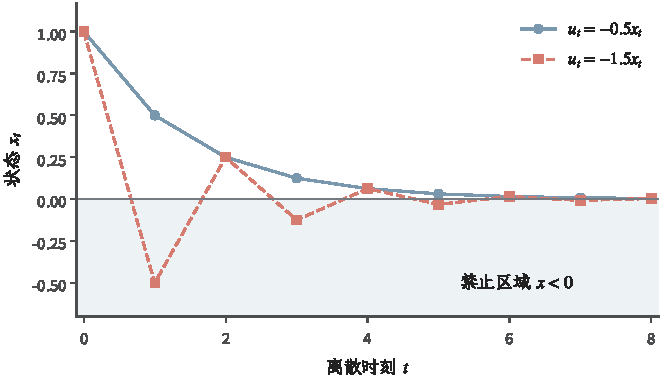
\includegraphics[width=\linewidth]{figures/math-preparation/dynamics/stability-safety.pdf}
  \caption{教学系统$x_{t+1}=x_t+u_t$从$x_0=1$出发。蓝色圆点采用$u_t=-0.5x_t$，
  保持$x_t\geq0$；红色方点采用$u_t=-1.5x_t$，第一步越过边界后交替衰减。
  两条轨迹都渐近稳定，只有前者保持安全集合$[0,\infty)$。灰色区域表示禁止的负半轴。}
  \label{fig:control-stability-safety}
\end{figure}

\subsection{控制屏障函数与可行动作}
安全函数$h$把状态是否允许转成一个标量符号，但$h$不必等于到边界的几何距离。
要判断动作会不会把状态推出集合，应观察$h$沿系统速度变化的速率。链式法则把它拆成
无控制漂移与控制引起的两部分，分别记为\term{Lie导数}（Lie derivative）：
\[
  L_{\bm{f}}h(\bm{x})
  =
  \nabla h(\bm{x})^{\top}\bm{f}(\bm{x}),
  \qquad
  L_{\bm{G}}h(\bm{x})
  =
  \nabla h(\bm{x})^{\top}\bm{G}(\bm{x}).
\]
本章把连续、严格递增、局部Lipschitz且满足$\alpha(0)=0$的函数$\alpha:\mathbb{R}\to\mathbb{R}$称为扩展类$\mathcal{K}$函数。局部Lipschitz条件保证下文标量比较系统的解局部唯一。常用选择是$\alpha(r)=\gamma r$，其中$\gamma>0$。
\begin{definition}[零化控制屏障函数]
\label{def:control-cbf}
若在某个包含$S$的开区域$D$内，对每个$\bm{x}$都有
\begin{equation}
  \sup_{\bm{u}\in U}
  \left\{
    L_{\bm{f}}h(\bm{x})
    +
    L_{\bm{G}}h(\bm{x})\bm{u}
  \right\}
  \geq
  -\alpha(h(\bm{x})),
  \label{eq:control-cbf-existence}
\end{equation}
并且上述上确界能够由某个$\bm{u}\in U$取到，则称$h$为区域$D$上的控制屏障函数（control barrier function, CBF）。
\end{definition}
这一条件及其基于二次规划的安全控制构造可参见控制屏障函数的系统论述\scite{math-ames2017cbf}
当$U$紧且花括号内的函数关于动作连续时，上确界能够取到；若这些条件不成立，只有上确界的数值不小于阈值，仍可能找不到真正满足约束的动作。定义保证每个状态至少存在一个安全动作，但实际反馈还必须从可行动作集合
\begin{equation}
  K_{\mathrm{cbf}}(\bm{x})
  =
  \left\{
    \bm{u}\in U:
    L_{\bm{f}}h(\bm{x})
    +
    L_{\bm{G}}h(\bm{x})\bm{u}
    \geq
    -\alpha(h(\bm{x}))
  \right\}
  \label{eq:control-cbf-action-set}
\end{equation}
中作出足够规则的选择。
\begin{theorem}[CBF条件保证正向不变]
\label{thm:control-cbf-invariance}
设式~\eqref{eq:control-affine-system}与式~\eqref{eq:control-safe-set}满足上述正则条件。若反馈$\bm{u}=\kappa(\bm{x})$局部Lipschitz，并对开区域$D$内每个状态满足$\kappa(\bm{x})\in K_{\mathrm{cbf}}(\bm{x})$，则$S$在相应闭环解存在的时间区间内正向不变。
\end{theorem}
\begin{proof}
沿任意闭环解令$r(t)=h(\bm{x}(t))$。链式法则与CBF约束给出
\[
  \dot r(t)
  \geq
  -\alpha(r(t)).
\]
考虑标量比较系统
\[
  \dot z(t)=-\alpha(z(t)),
  \qquad z(0)=r(0)\geq0.
\]
由于$\alpha$局部Lipschitz且$\alpha(0)=0$，标量比较系统在其最大存在区间内解唯一，$z=0$是平衡解；从非负初值出发的$z(t)$因而不能穿过零点。在闭环轨迹位于$D$且解存在的任意时间区间内，标量比较原理给出$r(t)\geq z(t)\geq0$。又因为$D$是包含$S$的开区域，轨迹若要离开$S$，必先在$D$内穿过$h=0$进入$h<0$，这与上述比较结论矛盾。因此$\bm{x}(t)\in S$在闭环解存在的全部时间内成立。

对最常用的$\alpha(r)=\gamma r$，结论可以直接验证：
\[
  \frac{\mathrm{d}}{\mathrm{d}t}
  \left(e^{\gamma t}r(t)\right)
  =
  e^{\gamma t}(\dot r(t)+\gamma r(t))
  \geq0.
\]
故$r(t)\geq e^{-\gamma t}r(0)\geq0$。边界上$r=0$时，该约束退化为$\dot r\geq0$，与式~\eqref{eq:control-nagumo-boundary}一致。
\end{proof}
该定理给出的是闭环轨迹性质，不只是某一步动作看起来朝向内部。证明依赖约束始终可行、反馈与动态具有足够正则性，以及控制信号按连续时间模型实际施加。缺少其中任一项，导数不等式都未必能沿真实轨迹成立。
\subsection{安全动作投影与二次规划}
设$\bm{u}_{\mathrm{nom}}(\bm{x})$是为性能设计的已有控制器，例如LQR反馈。可以在每个状态求解
\begin{equation}
  \begin{aligned}
    \bm{u}^{\ast}(\bm{x})
    \in\argmin_{\bm{u}\in U}\quad&
      \frac12
      (\bm{u}-\bm{u}_{\mathrm{nom}})^{\top}
      \bm{H}
      (\bm{u}-\bm{u}_{\mathrm{nom}})\\
    \text{s.t.}\quad&
      L_{\bm{f}}h(\bm{x})
      +
      L_{\bm{G}}h(\bm{x})\bm{u}
      \geq
      -\alpha(h(\bm{x})),
  \end{aligned}
  \label{eq:control-cbf-qp}
\end{equation}
其中$\bm{H}\succ\bm{0}$规定修改不同控制分量的代价。对控制仿射系统，CBF条件关于$\bm{u}$是线性不等式；若$U$是非空闭凸集，这就是具有闭凸可行域的凸二次规划。目标只表示“在该度量下尽量接近名义动作”，不表示修改后的控制仍保持原LQR成本最优。
\begin{example}[一维积分器上的安全投影]
\label{ex:control-cbf-scalar-projection}
考虑$\dot x=u$与安全集合$S=[0,\infty)$，取$h(x)=x$和$\alpha(h)=\gamma h$，其中$\gamma>0$。因为$L_fh=0$、$L_gh=1$，CBF条件正好是
\[
  u\geq-\gamma x.
\]
若$U=\mathbb{R}$、$H=1$，式~\eqref{eq:control-cbf-qp}的解是把标量名义动作投影到半直线$[-\gamma x,\infty)$：
\begin{equation}
  u^{\ast}(x)
  =
  \max\{u_{\mathrm{nom}}(x),-\gamma x\}.
  \label{eq:control-cbf-scalar-projection}
\end{equation}
例如$x=0.2$、$\gamma=1$且$u_{\mathrm{nom}}=-1$时，安全修正为$u^{\ast}=-0.2$，并使$\dot h=-h$；状态按$x(t)=0.2e^{-t}$接近边界但不穿过。若执行器还要求$u\leq-0.5$，则此状态下输入约束与CBF条件不相容，QP不可行。可行性取决于安全要求、当前状态与执行器能力的联合关系，不能由$h$的形式单独保证。
\end{example}

在$U$非空闭凸的上述条件下，若QP可行，则可行域非空且闭；正定二次目标具有强制性，因而最优解存在，严格凸性进一步保证最优动作唯一。若不要求可行域闭，严格凸性只能说明已有最优解至多一个，不能保证下确界能够取到。即使最优动作存在且唯一，也不自动意味着映射$\bm{x}\mapsto\bm{u}^{\ast}(\bm{x})$局部Lipschitz。活跃约束切换、约束梯度退化或可行域突变都可能破坏反馈正则性；要调用定理~\ref{thm:control-cbf-invariance}，还需用约束资格条件和参数化优化结果核对所选解的连续性或局部Lipschitz性质。
\begin{example}[圆形障碍外的安全修正]
\label{ex:control-cbf-obstacle}
考虑平面单积分器$\dot{\bm{p}}=\bm{u}$，要求位置留在圆形障碍外。令障碍中心为$\bm{c}$、半径为$r>0$，取
\[
  h(\bm{p})
  =
  \lVert\bm{p}-\bm{c}\rVert_2^2-r^2.
\]
安全集合是$h\geq0$。选择$\alpha(h)=\gamma h$后，CBF约束为
\begin{equation}
  2(\bm{p}-\bm{c})^{\top}\bm{u}
  \geq
  -\gamma
  \bigl(
    \lVert\bm{p}-\bm{c}\rVert_2^2-r^2
  \bigr).
  \label{eq:control-cbf-obstacle-constraint}
\end{equation}
在边界点$\bm{p}-\bm{c}=(r,0)^{\top}$处，若名义控制$\bm{u}_{\mathrm{nom}}=(-v,0)^{\top}$且$v>0$，它会直接指向障碍内部，因为左侧为$-2rv<0$。取$\bm{H}=\bm{I}$且没有其他输入约束时，二次规划把名义动作正交投影到半空间$2(\bm{p}-\bm{c})^{\top}\bm{u}\geq0$；在该边界点，修正结果为$\bm{u}^{\ast}=\bm{0}$。若名义动作还含切向分量，投影会保留切向分量，只移除指向障碍内部的法向分量。
\end{example}
多个安全条件$h_i(\bm{x})\geq0$可以产生多条线性约束，但每条单独可行不代表它们与执行器限制联合可行。两个障碍可能把系统夹在没有允许动作的位置；速度、转角或推力上限也可能阻止及时避让。加入松弛变量能够让优化器总有数值解，却同时允许违反安全约束。若这样做，松弛后的QP不再提供原来的硬不变性保证，必须明确新的故障处理或恢复区域。
图~\ref{fig:control-barrier-projection}将一维安全动作集合画在$(x,u)$平面。
对每个固定状态，可行域是一条竖直半直线；QP只需把名义动作投影到这条半直线上。
在远离边界的$x\geq1$处，名义动作$-1$本身可行；接近边界时，投影把它抬到$-x$。
动作修正由可行域决定，目标函数只规定在可行域中选择哪一个动作。

\begin{figure}[htbp]
  \centering
  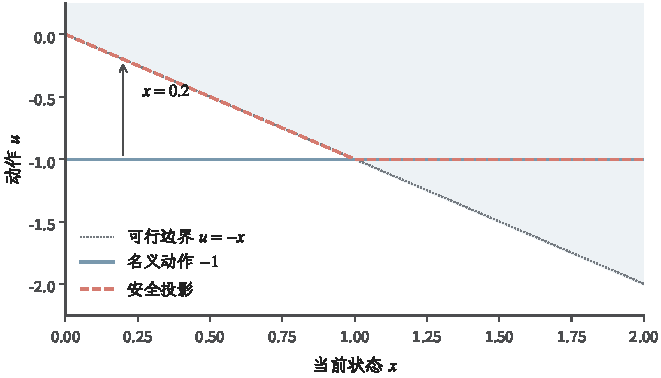
\includegraphics[width=\linewidth]{figures/math-preparation/dynamics/barrier-projection.pdf}
  \caption{教学积分器$\dot x=u$、安全集合$x\geq0$及$\alpha(h)=h$。
  灰色虚线是可行域边界$u=-x$，其上方阴影表示允许动作；蓝色实线为名义动作$u=-1$，
  红色虚线为投影$u^\star=\max\{-1,-x\}$。在$x=0.2$处，原动作修正为$-0.2$。
  此图假设无额外执行器约束，不能用来判断有限输入范围下的联合可行性。}
  \label{fig:control-barrier-projection}
\end{figure}

\subsection{鲁棒性、采样执行与高相对阶}
若真实动态含有有界加性扰动
\[
  \dot{\bm{x}}
  =
  \bm{f}(\bm{x})+\bm{G}(\bm{x})\bm{u}
  +\bm{d},
  \qquad
  \lVert\bm{d}\rVert_2\leq\delta,
\]
则最坏方向可使$\dot h$减少$\lVert\nabla h(\bm{x})\rVert_2\delta$。一个鲁棒充分条件是
\begin{equation}
  L_{\bm{f}}h
  +
  L_{\bm{G}}h\,\bm{u}
  \geq
  -\alpha(h)
  +
  \lVert\nabla h\rVert_2\delta.
  \label{eq:control-robust-cbf}
\end{equation}
模型误差也可在已有有效上界时并入类似裕量。没有经过验证的误差界时，任意加一个“安全系数”只能形成经验缓冲，不能推出鲁棒不变性。

数字控制器通常每隔$\Delta$秒求一次动作，并在两次更新之间保持不变。采样时刻满足CBF约束，不自动保证区间内部也满足，因为状态、Lie导数和最危险动作可能在区间中变化。可行做法包括用Lipschitz界为采样间变化预留裕量、直接建立离散时间屏障条件
\[
  h(\bm{x}_{t+1})-h(\bm{x}_t)
  \geq-\alpha_{\mathrm d}(h(\bm{x}_t)),
\]
其中离散比较函数应对每个$r\geq0$满足
$0\leq\alpha_{\mathrm d}(r)\leq r$。这样，只要
$h(\bm{x}_t)\geq0$，就有
\[
  h(\bm{x}_{t+1})
  \geq
  h(\bm{x}_t)-\alpha_{\mathrm d}(h(\bm{x}_t))
  \geq0,
\]
从而可以逐步归纳安全性。常用线性选择是
$\alpha_{\mathrm d}(r)=\gamma r$，其中$0<\gamma\leq1$。另一种做法是在预测时域内验证整段轨迹。连续时间证明不能省略这一实现差异。

还有一类问题来自\term{相对阶}。若$L_{\bm{G}}h(\bm{x})=\bm{0}$，控制不出现在$h$的一阶导数中，式~\eqref{eq:control-cbf-action-set}便无法限制动作。例如双积分器
\[
  \dot p=v,\qquad \dot v=u
\]
若用$h(p)=p-p_{\min}$保护位置下界，则$\dot h=v$与$u$无关，控制要到$\ddot h=u$才出现。该位置输出相对于输入具有相对阶$2$：第一次求导仍由现有速度决定，第二次才显露当前动作。
此时需使用高阶CBF，递归约束$h,\dot h$及更高导数，或把速度制动距离纳入安全函数。
例如$p-p_{\min}=0.1$、$v=-1$且最大制动加速度为$u=2$，最快停止所需距离为
$v^2/(2u)=0.25$，已经超过剩余距离。此刻即使位置仍在$S$内，也无法保证将来不越界。
这说明安全初态往往还要限制速度；只把位置约束写进一阶公式无法表达制动能力。把一阶公式机械套到$L_{\bm{G}}h=0$的情形，只会得到与控制无关的条件。

CBF还假设控制器知道用于计算$h$的状态。若只有带误差的状态估计，应对估计误差建立集合界或概率模型，再收紧安全集或构造输出反馈屏障。把估计值直接当作真实状态代入，只能证明估计轨迹满足约束，不能自动证明真实轨迹安全。
\section{用连续时间价值方程验证最优反馈}
\label{sec:control-hjb}

离散LQR与一般Bellman方程使用同一个跨时刻价值原则。
本节把时间步缩短，得到连续时间的价值方程；确定性漂移产生一阶项，扩散噪声增加二阶项。
光滑价值允许经典验证，折点与状态边界则需要更广义的解概念，并须重新核对边界条件。
\subsection{确定性HJB方程与验证定理}
有限时域LQR利用离散Bellman递推。连续时间中没有固定的一步，但可以把任意短区间$[t,t+\Delta]$视为第一步。考虑确定性受控系统
\begin{equation}
  \dot{\bm{x}}(s)
  =
  \bm{f}(\bm{x}(s),\bm{u}(s),s),
  \qquad
  \bm{x}(t)=\bm{x},
  \label{eq:control-continuous-dynamics}
\end{equation}
以及成本
\begin{equation}
  J_{t,\bm{x}}(\bm{u})
  =
  \phi(\bm{x}(T))
  +
  \int_t^T
  \ell(\bm{x}(s),\bm{u}(s),s)\,\mathrm{d}s.
  \label{eq:control-continuous-cost}
\end{equation}
价值函数为$V(\bm{x},t)=\inf_{\bm{u}}J_{t,\bm{x}}(\bm{u})$。控制$\bm{u}(s)$只能依据时刻$s$已经可用的信息；确定性完全状态反馈下，这通常表示它由当前或过去状态决定，而不能预知未来扰动。

动态规划原理把最优成本拆成短区间成本与剩余价值：
\begin{equation}
  V(\bm{x},t)
  =
  \inf_{\bm{u}|_{[t,t+\Delta]}}
  \left\{
    \int_t^{t+\Delta}
    \ell(\bm{x}(s),\bm{u}(s),s)\,\mathrm{d}s
    +
    V(\bm{x}(t+\Delta),t+\Delta)
  \right\}.
  \label{eq:control-continuous-dpp}
\end{equation}
下面给出经典形式推导。除假设$V$连续可微外，还假设动态规划原理成立，$\bm{f}$与$\ell$具有使短时轨迹偏移为$O(\Delta)$的连续性，并且短区间下确界可由可测的$\eta\Delta$-最优控制逼近，相关Taylor余项对这些控制局部一致。先在短区间内取任意常值动作$\bm{u}$。Taylor展开给出
\begin{align*}
  V(\bm{x}(t+\Delta),t+\Delta)
  &=
  V(\bm{x},t)
  +
  \Delta\,\partial_t V(\bm{x},t)\\
  &\quad+
  \Delta\,
  \nabla_{\bm{x}}V(\bm{x},t)^{\top}
  \bm{f}(\bm{x},\bm{u},t)
  +o(\Delta),
\end{align*}
而阶段积分为$\Delta\ell(\bm{x},\bm{u},t)+o(\Delta)$。由于式~\eqref{eq:control-continuous-dpp}对全部短时控制取下确界，代入这个常值动作只能先得到
\[
  -\partial_tV(\bm{x},t)
  \leq
  \ell(\bm{x},\bm{u},t)
  +
  \nabla_{\bm{x}}V(\bm{x},t)^{\top}
  \bm{f}(\bm{x},\bm{u},t).
\]
该式对每个$\bm{u}\in U$成立，故左侧不大于右侧对动作的下确界。

还需证明反向不等式。对任意$\eta>0$，在长度为$\Delta$的短区间上选择一个目标值距离下确界不超过$\eta\Delta$的允许控制。沿这条短时轨迹展开阶段成本和剩余价值，并利用每个时刻的Hamilton量都不小于其对动作的下确界，可得
\[
  \partial_tV(\bm{x},t)
  +
  \inf_{\bm{u}\in U}
  \left\{
    \ell(\bm{x},\bm{u},t)
    +
    \nabla_{\bm{x}}V(\bm{x},t)^{\top}
    \bm{f}(\bm{x},\bm{u},t)
  \right\}
  \leq
  \eta+o(1).
\]
依次令$\Delta\downarrow0$和$\eta\downarrow0$便得到反向不等式。两边合并，得到
\term{Hamilton--Jacobi--Bellman方程}：
\begin{equation}
  -\partial_tV(\bm{x},t)
  =
  \inf_{\bm{u}\in U}
  \left\{
    \ell(\bm{x},\bm{u},t)
    +
    \nabla_{\bm{x}}V(\bm{x},t)^{\top}
    \bm{f}(\bm{x},\bm{u},t)
  \right\},
  \qquad
  V(\bm{x},T)=\phi(\bm{x}).
  \label{eq:control-deterministic-hjb}
\end{equation}
花括号内的量常称为控制问题的Hamilton量，它把瞬时成本与价值沿当前速度的变化率相加，再对动作作局部优化。它不是第~\ref{chap:dynamical-systems-and-state-estimation}章Hamilton系统中沿轨迹守恒的能量函数；二者名称相近，所描述的对象和方程不同。这里采用成本最小化约定，所以写$\inf$和$-\partial_tV$；若改为奖励最大化，符号必须成套改变\scite{math-bardi1997hjb}
\begin{theorem}[确定性HJB验证定理]
\label{thm:control-hjb-verification}
设$V\in C^1$满足式~\eqref{eq:control-deterministic-hjb}及终端条件，并假设任意允许控制都产生存在到$T$的轨迹。若存在可实现反馈$\bm{u}^{\ast}=\kappa(\bm{x},t)$逐点达到HJB右侧的下确界，且相应闭环轨迹存在，则$V$等于最优价值，$\kappa$是最优反馈。
\end{theorem}
\begin{proof}
任取一个允许控制$\bm{u}(s)$及其轨迹。HJB中的下确界不大于代入该动作后的值，所以
\[
  \partial_sV(\bm{x}(s),s)
  +
  \nabla_{\bm{x}}V(\bm{x}(s),s)^{\top}
  \bm{f}(\bm{x}(s),\bm{u}(s),s)
  +
  \ell(\bm{x}(s),\bm{u}(s),s)
  \geq0.
\]
链式法则把前两项合成$\mathrm{d}V(\bm{x}(s),s)/\mathrm{d}s$。从$t$积分到$T$，并用$V(\bm{x}(T),T)=\phi(\bm{x}(T))$，得到
\[
  J_{t,\bm{x}}(\bm{u})
  \geq V(\bm{x},t).
\]
因此$V$是所有允许控制成本的共同下界。

采用$\bm{u}^{\ast}=\kappa(\bm{x},s)$时，反馈在每一点达到HJB下确界，上述不等式处处取等号。沿闭环轨迹积分便有$J_{t,\bm{x}}(\bm{u}^{\ast})=V(\bm{x},t)$。所以该反馈达到共同下界，$V$就是最优价值。
\end{proof}
HJB方程是最优性的局部必要关系；验证定理则说明一个足够光滑的候选解如何成为全局证书。仅把偏微分方程在若干采样点上的残差降得很小，还不能自动获得验证结论，因为还需终端或边界条件、可实现的极小动作、轨迹存在性以及整个相关区域上的方程关系。
\subsection{随机HJB方程与扩散生成元}
若状态服从Itô随机微分方程
\begin{equation}
  \mathrm{d}\bm{X}_s
  =
  \bm{f}(\bm{X}_s,\bm{u}_s,s)\,\mathrm{d}s
  +
  \bm{\Sigma}(\bm{X}_s,\bm{u}_s,s)\,
  \mathrm{d}\bm{W}_s,
  \label{eq:control-stochastic-dynamics}
\end{equation}
控制$\bm{u}_s$必须对当前滤过适应，不能使用未来布朗增量。价值改为期望成本的下确界。对$V\in C^{2,1}$使用第~\ref{chap:dynamical-systems-and-state-estimation}章的Itô公式，短时间条件期望中一阶随机积分均值为零，二次变差留下
\[
  \frac12
  \operatorname{tr}
  \left(
    \bm{\Sigma}\bm{\Sigma}^{\top}
    \nabla_{\bm{x}}^2V
  \right).
\]
因此随机HJB为
\begin{equation}
  \begin{aligned}
  -\partial_tV(\bm{x},t)
  =
  \inf_{\bm{u}\in U}
  \biggl\{&
    \ell(\bm{x},\bm{u},t)
    +
    \nabla_{\bm{x}}V(\bm{x},t)^{\top}
    \bm{f}(\bm{x},\bm{u},t)\\
    &+
    \frac12
    \operatorname{tr}
    \left[
      \bm{\Sigma}(\bm{x},\bm{u},t)
      \bm{\Sigma}(\bm{x},\bm{u},t)^{\top}
      \nabla_{\bm{x}}^2V(\bm{x},t)
    \right]
  \biggr\},
  \end{aligned}
  \label{eq:control-stochastic-hjb}
\end{equation}
终端条件仍为$V(\bm{x},T)=\phi(\bm{x})$。

\begin{theorem}[随机HJB验证]
\label{thm:control-stochastic-hjb-verification}
设$V$对时间一次、对状态二次连续可微，满足式~\eqref{eq:control-stochastic-hjb}及终端条件。假设每个允许的适应控制都使式~\eqref{eq:control-stochastic-dynamics}存在到$T$，成本和下述Itô各项可积，并且随机积分是真鞅。若存在可容许的反馈$\bm{u}^{\ast}=\kappa(\bm{x},t)$逐点达到HJB中的下确界，则$V$等于最优期望成本，$\kappa$是最优反馈。
\end{theorem}
\begin{proof}
记动作$\bm{u}$下的受控生成元为
\[
  \mathcal{L}^{\bm{u}}V
  =
  \nabla_{\bm{x}}V^{\top}\bm{f}
  +
  \frac12
  \operatorname{tr}
  \left(
    \bm{\Sigma}\bm{\Sigma}^{\top}
    \nabla_{\bm{x}}^2V
  \right).
\]
HJB说明，对任意允许动作都有
\[
  \partial_sV+\mathcal{L}^{\bm{u}_s}V
  +\ell(\bm{X}_s,\bm{u}_s,s)\geq0.
\]
沿受控轨迹对$V(\bm{X}_s,s)$使用Itô公式，从$t$积分到$T$并取条件期望。随机积分因真鞅条件期望为零，故
\[
  \mathbb{E}\left[
    \phi(\bm{X}_T)
    +
    \int_t^T
      \ell(\bm{X}_s,\bm{u}_s,s)\,\mathrm{d}s
    \,\middle|\,\bm{X}_t=\bm{x}
  \right]
  \geq V(\bm{x},t).
\]
所以$V$是所有允许控制期望成本的下界。对反馈$\kappa$，HJB下确界逐点达到，上述生成元不等式取等号；重复同一计算便得到其期望成本恰为$V(\bm{x},t)$，从而完成验证。
\end{proof}
若随机积分只是局部鞅，直接断言其期望为零可能失败；通常需要增长界、停时局部化与一致可积性等条件把局部结论提升为上述等式。随机HJB的局部形式本身不能替代这些可积性检查。

若扩散矩阵与动作无关，且价值是二次函数，二阶项可能只增加与状态无关的常数，这与离散LQR中式~\eqref{eq:control-lqr-noise-constant}的现象一致。若$\bm{\Sigma}$依赖动作或状态，二阶项会参与动作最小化或改变价值的状态形状，反馈一般也会改变。
\subsection{连续时间LQR与微分Riccati方程}
用HJB重新考察线性二次问题。令
\[
  \dot{\bm{x}}
  =
  \bm{A}\bm{x}+\bm{B}\bm{u},
\]
阶段成本和终端成本分别为
\[
  \ell(\bm{x},\bm{u})
  =
  \bm{x}^{\top}\bm{Q}\bm{x}
  +
  \bm{u}^{\top}\bm{R}\bm{u},
  \qquad
  \phi(\bm{x})
  =
  \bm{x}^{\top}\bm{Q}_T\bm{x},
\]
其中$\bm{Q},\bm{Q}_T\succeq\bm{0}$、$\bm{R}\succ\bm{0}$。设
\[
  V(\bm{x},t)
  =
  \bm{x}^{\top}\bm{P}(t)\bm{x},
  \qquad
  \bm{P}(T)=\bm{Q}_T,
\]
并取$\bm{P}(t)$对称。于是
\[
  \partial_tV
  =
  \bm{x}^{\top}\dot{\bm{P}}(t)\bm{x},
  \qquad
  \nabla_{\bm{x}}V
  =
  2\bm{P}(t)\bm{x}.
\]
代入确定性HJB，动作相关项为
\[
  \bm{u}^{\top}\bm{R}\bm{u}
  +
  2\bm{x}^{\top}\bm{P}\bm{B}\bm{u}.
\]
同样配方：
\begin{align*}
  &\bm{u}^{\top}\bm{R}\bm{u}
  +
  2\bm{x}^{\top}\bm{P}\bm{B}\bm{u}\\
  &\quad=
  \left(
    \bm{u}+\bm{R}^{-1}\bm{B}^{\top}\bm{P}\bm{x}
  \right)^{\top}
  \bm{R}
  \left(
    \bm{u}+\bm{R}^{-1}\bm{B}^{\top}\bm{P}\bm{x}
  \right)
  -
  \bm{x}^{\top}
  \bm{P}\bm{B}\bm{R}^{-1}\bm{B}^{\top}\bm{P}
  \bm{x}.
\end{align*}
所以最优反馈为
\begin{equation}
  \bm{u}^{\ast}(t)
  =
  -\bm{R}^{-1}\bm{B}^{\top}\bm{P}(t)\bm{x}(t),
  \label{eq:control-continuous-lqr-gain}
\end{equation}
而对任意$\bm{x}$比较二次型系数，得到
\begin{equation}
  -\dot{\bm{P}}
  =
  \bm{Q}
  +
  \bm{A}^{\top}\bm{P}
  +
  \bm{P}\bm{A}
  -
  \bm{P}\bm{B}\bm{R}^{-1}\bm{B}^{\top}\bm{P},
  \qquad
  \bm{P}(T)=\bm{Q}_T.
  \label{eq:control-continuous-riccati}
\end{equation}
这就是连续时间微分Riccati方程。它从终端条件向较早时刻反向积分；式中的负号反映价值边界给在终点，而不是数值积分器可以任意忽略的记号。

无限时域稳态令$\dot{\bm{P}}=\bm{0}$，得到连续代数Riccati方程
\begin{equation}
  \bm{0}
  =
  \bm{Q}
  +
  \bm{A}^{\top}\bm{P}
  +
  \bm{P}\bm{A}
  -
  \bm{P}\bm{B}\bm{R}^{-1}\bm{B}^{\top}\bm{P}.
  \label{eq:control-care}
\end{equation}
此时稳定的含义改为闭环矩阵$\bm{A}-\bm{B}\bm{R}^{-1}\bm{B}^{\top}\bm{P}$的全部特征值实部为负。在连续时间版本的可稳定、可检测条件下，选取半正定稳定化解可得到无限时域最优反馈。离散DARE和连续CARE外形相近，却分别对应单位圆和左半平面的稳定区域，不能混用。
\subsection{非光滑价值、边界条件与部分观测}
经典HJB推导假设价值足够光滑，但最优控制常产生切换面、状态约束或不可微终端成本。
此时价值可能连续，却没有处处可用的梯度或Hessian矩阵。困难在于方程含有导数，不能
把一个折点直接代入经典公式。\term{黏性解}（viscosity solution）用光滑函数从上下两侧
接触价值，在接触点检验方程的不等式；导数取自接触函数，价值本身可以没有导数。

为固定不等式方向，将前面的确定性HJB写成
\[
  F(\bm x,t,a,\bm p)
  :=-a-\inf_{\bm u\in U}\{\ell(\bm x,\bm u,t)
                       +\bm p^\top\bm f(\bm x,\bm u,t)\}=0,
\]
其中$a$和$\bm p$分别代表时间导数与状态梯度。
\begin{definition}[连续价值函数的黏性解]
  \label{def:control-viscosity-solution}
  设$V$在HJB作用域内连续。若对任意光滑测试函数$\varphi$，当$V-\varphi$在
  内点$(\bm x,t)$取得局部最大值时，都有
  $F(\bm x,t,\partial_t\varphi,\nabla\varphi)\leq0$，称$V$为黏性次解。
  若局部最小值处都满足相应的$F\geq0$，称为黏性上解。
  同时满足两项，且按当前问题满足终端或边界条件的$V$，称为黏性解。
\end{definition}
测试函数可平移一个常数，使接触时$V=\varphi$。局部最大意味着测试函数在邻域内
位于价值上方并与之接触，局部最小则对应位于价值下方的接触；测试函数的导数必须
符合这个局部接触条件。
随机二阶HJB还要把测试函数的Hessian代入$F$。当$V$足够光滑时，取$\varphi=V$
便同时得到$F\leq0$与$F\geq0$，恢复经典等式。在适当函数类和边界条件下，比较原理
使每个次解不高于每个上解，从而给出唯一性；比较原理本身仍有连续性、增长与方程结构
条件，不能由这个定义自动推出。

一维最短到达问题说明为什么必须先区分延续域与目标边界。令$\dot x=u$、$|u|\leq1$，每经过一单位时间支付成本$1$，到达目标集合$\{0\}$时终止。最短到达时间是
\[
  V(x)=|x|.
\]
在$x\neq0$处，稳态HJB为
\[
  0
  =
  1+\inf_{|u|\leq1}V'(x)u
  =
  1-|V'(x)|,
\]
最优控制分别取$u=-1$和$u=1$，把左右两侧的状态推向原点。价值在$x=0$处没有经典导数，但$x=0$是退出目标边界，不属于延续域$\mathbb{R}\setminus\{0\}$；HJB在两个延续分支上都由经典导数满足，目标点只需施加$V(0)=0$的边界条件。因此，这个例子说明全局价值可以在目标边界非光滑，却不能单独证明延续域内部必须使用黏性解。只有当切换面、状态约束或非光滑终端数据使折点落在方程作用域内时，才需要用上方或下方的光滑测试函数解释该点的HJB不等式；相应唯一性仍依赖当前边界条件、函数增长类和Hamilton量的比较原理。

\begin{example}[延续域内部的价值折点]
  \label{ex:control-viscosity-interior-kink}
  仍取$\dot x=u$、$|u|\leq1$，但不在到达原点时退出：固定终点$T$，运行成本为零，
  终端成本为$|x(T)|$。从$(x,t)$出发最多移动$T-t$的距离，因此
  \[
    V(x,t)=\max\{|x|-(T-t),0\}.
  \]
  在$|x|<T-t$时可以到达原点并停留，价值为零；在外侧，剩余时间只能减去$T-t$
  的距离。HJB为$-V_t+|V_x|=0$，终端条件为$V(x,T)=|x|$。
  折点$x=\pm(T-t)$位于延续域内部，经典导数在这里不存在。
  例如$T-t=1$时，$|x|\leq1$都能在终点前到达原点，价值为零；$x=1.5$的最低终端代价为$0.5$。
  $x=1$处的折角因此分开“时间足够完全纠正”和“仍有不可消除终端偏差”两类状态。

  以正侧折点为例，局部价值为$\max\{x+t-T,0\}$。从下方接触的光滑函数在接触点
  的导数对$(\varphi_x,\varphi_t)$属于$(p,p)$、$0\leq p\leq1$，对应两侧斜率的
  凸组合。因此$-\varphi_t+|\varphi_x|=-p+p=0$，满足上解条件。
  空间方向的向上折角使该点没有光滑的上方接触函数，次解检验在这里没有额外约束；
  光滑区域则由经典等式同时满足两项条件。负侧同理。
  这个可直接求出最优成本的例子说明，黏性条件确实能在方程作用域内部处理折点，
  而不需要把切换面误当作终止边界。
\end{example}

状态约束也需要边界条件。若边界不可穿越，价值只在可行控制存在的区域定义，HJB必须与可行方向或状态约束边界条件共同解释。若允许碰到边界后终止，则应给出退出成本。仅在区域内部求出一个光滑解，不能决定边界上的控制含义。

当真实状态不可见时，把$\bm{x}$直接作为HJB状态也不可实现。一般做法是把给定观测历史的条件状态分布作为\term{信念状态}；它包含当前决策所需的信息，但通常是无限维对象。线性高斯二次问题具有特殊的分离结构，可以用Kalman估计配合LQR反馈；一般部分观测、风险敏感或受约束问题则不能从分离原理直接推出最优性。

HJB、LQR和CBF之间也有清楚边界。HJB寻找指定成本下的最优反馈，CBF把安全性写成每个状态的动作可行约束。可以在HJB中加入状态约束，也可以用CBF-QP修正性能控制器，但前者需要求解受约束动态优化，后者通常牺牲原性能最优性。稳定价值函数、最优价值函数和屏障函数都沿轨迹考察标量变化，却分别证明收敛、最优和不变性，不能只因公式都含导数就互相替代。
\section{本章小结}
\label{sec:control-theory-summary}

控制把给定输入下的状态演化改成闭环选择问题。在线性系统中，可控性要求输入能够生成全部状态方向，可稳定性只要求输入能够改变不稳定模式；可观测性要求输出区分全部初态，可检测性只要求不可见模式自行稳定。秩判据给出有限时域的整体检查，PBH判据直接定位危险特征模式。可稳定与可检测共同支持观测器和状态反馈的分离设计，但这个结论依赖线性结构及相应信息条件。

有限时域LQR把线性动态、二次成本和Bellman递推闭合在二次价值函数族中。逐步配方给出线性反馈增益与Riccati反向递推；零均值独立加性噪声只增加价值常数项。本章的无折扣无限时域LQR改用确定性系统：它不能接受任意代数Riccati根，而要在可稳定、可检测及代价正定条件下选择半正定稳定化解。滤波Riccati与控制Riccati具有矩阵对偶结构；在标准线性高斯条件下，条件状态均值可以接入LQR反馈而保持期望成本最优，但信息、噪声或约束改变后必须重新验证分离。

成本最优不等于安全。正向不变性要求每条闭环轨迹持续留在允许集合内；CBF将边界方向条件扩展为集合附近的动作不等式，并可通过二次规划最小修改名义控制器。该保证以动作约束可行、反馈正则、状态信息可靠和连续模型与实际执行一致为前提。扰动、模型误差、采样保持、输入上限和高相对阶都会改变需要验证的条件。

连续时间Bellman原理在短时间极限下产生HJB方程；随机动态借助Itô公式多出扩散的二阶项。验证定理把HJB解、达到极小值的反馈和全时域最优性连接起来，连续时间LQR则把这一关系化为微分与代数Riccati方程。价值在HJB作用域内非光滑时需要黏性解等广义概念，目标边界上的非光滑则要与边界条件一同解释；部分观测需要信念状态或具有专门分离结构的估计器。由此可以区分本章的三类保证：稳定性控制长期衰减，最优性比较累计成本，安全性保持允许集合；完整的受控系统往往需要同时核对三者。

第~\ref{chap:game-theory-and-multi-agent-decision}章将放开“环境规律与其他参与者策略固定”
这一前提，研究多方同时调整行动时的响应、均衡与学习保证。

\chapter{博弈论与多方决策}
\label{chap:game-theory-and-multi-agent-decision}

第~\ref{chap:decision-theory-and-dynamic-risk}章把环境规律看作给定条件，
第~\ref{chap:control-theory}章则让单个控制器通过反馈改变状态。多方决策进一步改变了
“其他行动规则固定”这一前提。若另一方也会观察、推断和
调整，当前行动的后果就取决于双方策略，而不能只对一个固定环境分布取期望。此时，
“哪个行动最好”必须改写为“面对其他参与者的选择，什么策略能够抵抗偏离或形成稳定响应”。
本章沿用一个三张牌的教学博弈。牌面只有高牌、中牌和低牌，实际使用其中一张隐藏牌来
决定是否质询、是否应对。这个小牌面会先被压缩成收益矩阵，用于求零和博弈值；随后还原
成历史树，说明私人信息为何不能当作普通状态。重复对局时，局部决策会产生遗憾，完全回忆
把这些局部遗憾连接到整局偏离。若参与者转为合作，同一个任务又会提出怎样按各方信息
分配共同收益的问题。
这几类答案不可互换。极小极大值控制最坏对手下的保证，Nash均衡排除单方有利偏离，
相关均衡还要说明看到建议后允许怎样改动；低遗憾是多轮比较结论，不自动说明末次策略
收敛；Shapley值分配预先定义的联盟价值，却不负责证明参与者会自愿采用该分配。本章
依次从收益结构、响应稳定性、信息结构、学习过程和合作分配五个方面建立这些边界。

\section{在零和对抗中求最坏对手下的保证}
\label{sec:game-matrix-zero-sum-duality}
\subsection{联合行动、混合策略与最佳响应}

\begin{definition}[有限矩阵博弈]
\label{def:game-finite-matrix-game}
有限双人\term{矩阵博弈}（matrix game）由两组非空有限行动
\(A_1=\{1,\ldots,m\}\)、\(A_2=\{1,\ldots,n\}\)和两张收益矩阵
\(\bm{U}_1,\bm{U}_2\in\mathbb{R}^{m\times n}\)给出。第1位参与者选择行，第2位
参与者选择列，落在\((i,j)\)时，两人的收益分别为
\(\bigl((\bm{U}_1)_{i,j},(\bm{U}_2)_{i,j}\bigr)\)。若存在矩阵\(\bm{M}\)使
\(\bm{U}_1=\bm{M}\)、\(\bm{U}_2=-\bm{M}\)，双方收益之和恒为零，就得到
\term{零和博弈}（zero-sum game）。
\end{definition}
一个人增加的收益正好是另一个人的损失，因此
零和情形只需记录第1位参与者的收益矩阵\(\bm{M}\)；一般和情形则不能省略第二张矩阵。

固定行动容易被对方针对，随机选择则把可预测的单一行动改成一个概率分布。
\begin{definition}[纯策略与混合策略]
\label{def:game-pure-mixed-strategy}
直接选择某一行或某一列称为\term{纯策略}（pure strategy）。在行动上选择概率分布
称为混合策略（mixed strategy）。记
\[
  \Delta_m
  =
  \left\{
    \bm{x}\in\mathbb{R}^m:
    \bm{x}\geq\bm{0},\
    \bm{1}^{\top}\bm{x}=1
  \right\}
\]
为\(m\)个行动上的概率单纯形。双方以各自的混合策略独立抽取行动。
\end{definition}
该单纯形嵌入\(\mathbb{R}^m\)，几何维数为\(m-1\)。在零和情形，第1位参与者采用
\(\bm{x}\in\Delta_m\)，第2位参与者采用
\(\bm{y}\in\Delta_n\)时，期望收益为
\begin{equation}
  u(\bm{x},\bm{y})
  =
  \bm{x}^{\top}\bm{M}\bm{y}.
  \label{eq:game-matrix-expected-payoff}
\end{equation}
混合策略不是在一局内把多个行动平均执行，而是在行动前用随机装置抽取一个纯行动。

\begin{definition}[最佳响应]
\label{def:game-best-response}
给定对手策略后，使自身期望收益最大的策略称为\term{最佳响应}（best response）。
在零和情形，第1位参与者面对\(\bm{y}\)的最佳响应集合为
\[
  \operatorname{BR}_1(\bm{y})
  =
  \argmax_{\bm{x}\in\Delta_m}
  \bm{x}^{\top}\bm{M}\bm{y}.
\]
\end{definition}
一般和矩阵博弈中，将上述目标中的$\bm M$换成自己的收益矩阵$\bm U_1$；
第2位参与者则最大化$\bm x^\top\bm U_2\bm y$，不能继续把对方收益简单取负。
线性目标总能在某个纯行动达到最大值，但把全部概率放在一个最佳纯行动上未必是唯一
选择；若多行并列，它们的任意混合仍是最佳响应。

\subsection{匹配硬币与混合策略}

考虑双方同时选择正面\(H\)或反面\(T\)。两面相同时参与者1得到\(1\)，不同时得到
\(-1\)，参与者2得到相反收益。参与者1的收益矩阵为
\[
  \bm{M}_{\mathrm{mp}}
  =
  \begin{pmatrix}
    1 & -1\\
    -1 & 1
  \end{pmatrix}.
\]
任意纯策略组合都不是稳定响应：若两面相同，参与者2改换一面便能改善；若两面不同，
参与者1改换一面便能改善。若逐轮对上一轮行动作纯最佳响应，行动还会在四个组合之间
循环，这说明“每轮都回应当前对手”不等于联合策略会收敛。

令参与者1选择\(H\)的概率为\(p\)，参与者2选择\(H\)的概率为\(q\)。参与者1选
\(H\)与\(T\)的期望收益分别为\(2q-1\)与\(1-2q\)。只有\(q=1/2\)能使两行
收益相同，避免参与者1利用某一面；对称地，只有\(p=1/2\)能使参与者2无法利用。
所以双方均匀随机化时收益为
\[
  (1/2,1/2)\bm{M}_{\mathrm{mp}}(1/2,1/2)^{\top}=0.
\]
这个二乘二例子展示了混合策略的核心作用：随机化不是让某个纯行动变好，而是消除对手
针对固定行动获得的优势。

图~\ref{fig:game-matching-best-responses}把双方最佳响应放到同一概率平面中。
给定纵坐标$q$，蓝线列出行方允许采用的最佳$p$；给定横坐标$p$，红线列出列方的
最佳$q$。各自单看一条响应仍不能选出联合结果；两条集合同时相交，才表示双方都在
回应对方。中心的整段响应保留了并列最优，因此这个均衡不要求“每个人有唯一最佳行动”。

\begin{figure}[htbp]
  \centering
  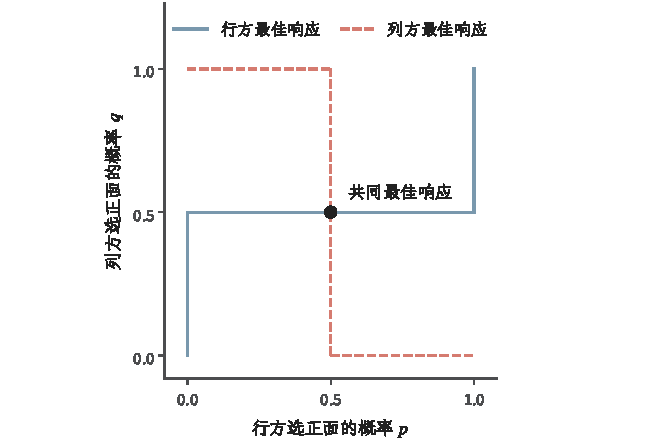
\includegraphics[width=\linewidth]{figures/math-preparation/dynamics/matching-best-responses.pdf}
  \caption{匹配硬币中的最佳响应对应。横轴$p$是行方选$H$的概率，纵轴$q$是列方选
  $H$的概率；蓝色实线表示行方最大化收益的最佳响应，红色虚线表示列方最小化行方收益
  的最佳响应。蓝线在$q=1/2$包含全部$p$，红线在$p=1/2$包含全部$q$，唯一交点
  为$(1/2,1/2)$。线段是最佳响应集合，不是随时间运行的学习轨迹。}
  \label{fig:game-matching-best-responses}
\end{figure}

\subsection{三张牌质询博弈}

考虑高牌\(H\)、中牌\(M\)和低牌\(L\)。庄家从\(H\)与\(L\)中等概率发给参与者1
一张隐藏牌，\(M\)留作公共比较基准。参与者1看到自己的牌后选择质询\(B\)或放弃
\(P\)。放弃时收益为\(0\)。质询后，参与者2只知道发生了质询，不知道隐藏牌，并选择
应对\(C\)或退让\(F\)。退让时参与者1得到\(1\)；应对时，高牌使参与者1得到\(2\)，
低牌使其得到\(-2\)。参与者2得到相反收益。

在把信息时序展开以前，可以先把一项纯策略写成“拿到高牌时做什么，拿到低牌时做什么”。
按\((P,P),(B,P),(P,B),(B,B)\)排列参与者1的四个完整计划，按\(F,C\)排列参与者2
的行动，参与者1的事前期望收益矩阵为
\begin{equation}
  \bm{M}
  =
  \begin{pmatrix}
    0 & 0\\
    1/2 & 1\\
    1/2 & -1\\
    1 & 0
  \end{pmatrix}.
  \label{eq:game-card-normal-form}
\end{equation}
例如，计划\((B,P)\)只在拿到高牌时质询。对方退让时，收益以一半概率为\(1\)、一半
概率为\(0\)，故矩阵元素为\(1/2\)；对方应对时，相应期望为\(1\)。

这个矩阵没有纯策略鞍点。每一行的最小收益依次为
\(0,1/2,-1,0\)，故第1位参与者先公开选行时至多保证\(1/2\)；每一列的最大收益
分别为\(1,1\)，故第2位参与者先公开选列时至多把收益压到\(1\)。两种次序得到不同
数值，说明任何固定纯行动都会留下可利用的响应。

\subsection{保证值与极小极大值}

第1位参与者在不知道对方将怎样响应时，希望最大化自己能够保证的最小收益：
\[
  \underline v
  =
  \max_{\bm{x}\in\Delta_m}
  \min_{\bm{y}\in\Delta_n}
  \bm{x}^{\top}\bm{M}\bm{y}.
\]
对固定\(\bm{x}\)，第2位参与者的目标关于\(\bm{y}\)线性，所以最小值在某个纯列
达到。因此
\[
  \min_{\bm{y}\in\Delta_n}
  \bm{x}^{\top}\bm{M}\bm{y}
  =
  \min_j(\bm{M}^{\top}\bm{x})_j.
\]
类似地，第2位参与者希望把第1位参与者的最大可得收益压低到
\[
  \overline v
  =
  \min_{\bm{y}\in\Delta_n}
  \max_{\bm{x}\in\Delta_m}
  \bm{x}^{\top}\bm{M}\bm{y}
  =
  \min_{\bm{y}\in\Delta_n}\max_i(\bm{M}\bm{y})_i.
\]

对任意\(\bm{x},\bm{y}\)，都有
\[
  \min_{\widetilde{\bm{y}}}
  u(\bm{x},\widetilde{\bm{y}})
  \leq
  u(\bm{x},\bm{y})
  \leq
  \max_{\widetilde{\bm{x}}}
  u(\widetilde{\bm{x}},\bm{y}).
\]
分别对左侧取最大、右侧取最小，得到
\(\underline v\leq\overline v\)。这只是弱极小极大关系。要证明有限零和博弈中
两者相等，还需要说明双方约束恰好构成一对线性规划。

\begin{theorem}[有限零和博弈的极小极大定理]
\label{thm:game-finite-minimax}
对任意有限收益矩阵\(\bm{M}\)，有
\begin{equation}
  \max_{\bm{x}\in\Delta_m}
  \min_{\bm{y}\in\Delta_n}
  \bm{x}^{\top}\bm{M}\bm{y}
  =
  \min_{\bm{y}\in\Delta_n}
  \max_{\bm{x}\in\Delta_m}
  \bm{x}^{\top}\bm{M}\bm{y}.
  \label{eq:game-minimax-equality}
\end{equation}
共同数值称为博弈值\(v^\star\)。等式两侧的最优解分别称为双方的极小极大策略。
\end{theorem}

\begin{proof}
引入第1位参与者要保证的收益下界\(v\)。条件
\((\bm{M}^{\top}\bm{x})_j\geq v\)对每一列成立，恰好表示任何纯列都不能把收益压到
\(v\)以下。第1位参与者的问题因此是
\begin{equation}
  \begin{aligned}
    \max_{\bm{x},v}\quad&v\\
    \text{s.t.}\quad&
      \bm{M}^{\top}\bm{x}\geq v\bm{1},\\
    &\bm{1}^{\top}\bm{x}=1,\qquad
      \bm{x}\geq\bm{0}.
  \end{aligned}
  \label{eq:game-row-player-lp}
\end{equation}
它的最优值正是\(\underline v\)。为第一组不等式引入非负乘子
\(\bm{y}\geq\bm{0}\)，为概率归一化引入自由乘子\(w\)。
把最大化问题写成上界形式后，其拉格朗日函数可整理为
\[
  \mathcal{L}(\bm{x},v;\bm{y},w)
  =
  v+\bm{y}^{\top}
  (\bm{M}^{\top}\bm{x}-v\bm{1})
  +w(1-\bm{1}^{\top}\bm{x}).
\]
若对自由变量\(v\)取上确界仍为有限值，必须有
\(\bm{1}^{\top}\bm{y}=1\)。若对\(\bm{x}\geq\bm{0}\)取上确界仍为有限值，
还必须有
\[
  \bm{M}\bm{y}\leq w\bm{1}.
\]
满足这些条件时，上确界等于\(w\)。于是对偶问题为
\begin{equation}
  \begin{aligned}
    \min_{\bm{y},w}\quad&w\\
    \text{s.t.}\quad&
      \bm{M}\bm{y}\leq w\bm{1},\\
    &\bm{1}^{\top}\bm{y}=1,\qquad
      \bm{y}\geq\bm{0}.
  \end{aligned}
  \label{eq:game-column-player-lp}
\end{equation}
它要求每个纯行的收益都不超过\(w\)，所以最优值正是\(\overline v\)。两个单纯形
都非空且紧，目标连续，因此式~\eqref{eq:game-row-player-lp}与
\eqref{eq:game-column-player-lp}都有有限最优解。第
\ref{thm:opt-lp-strong-duality}号定理给出原对偶最优值相等，即
\(\underline v=\overline v=v^\star\)。
\end{proof}

这个证明不只是交换了\(\max\)与\(\min\)。概率归一化把乘子变成对方的混合策略，
逐行动收益约束把对偶可行性变成“没有纯行动能突破当前上界”。强对偶才把两种单方
证书接成同一个博弈值。

若\(\bm{x}^\star\)与\(\bm{y}^\star\)分别是两侧最优策略，则对任意
\(\bm{x}\in\Delta_m\)、\(\bm{y}\in\Delta_n\)，
\begin{equation}
  u(\bm{x},\bm{y}^\star)
  \leq
  u(\bm{x}^\star,\bm{y}^\star)
  \leq
  u(\bm{x}^\star,\bm{y}).
  \label{eq:game-zero-sum-saddle}
\end{equation}
左侧来自\(\bm{y}^\star\)把所有行收益限制在\(v^\star\)以下，右侧来自
\(\bm{x}^\star\)对所有列保证至少\(v^\star\)。这就是混合策略上的鞍点条件。
博弈值由式~\eqref{eq:game-minimax-equality}唯一确定，但达到该值的策略可以不唯一；
把“值唯一”误读成“解唯一”，会遗漏并列最优行动形成的整个最优策略集合。

\subsection{牌面博弈的原对偶最优证书}

对式~\eqref{eq:game-card-normal-form}，令第1位参与者在计划
\((B,P)\)与\((B,B)\)上分别放置概率\(2/3\)与\(1/3\)，其余计划概率为零：
\[
  \bm{x}^\star
  =
  (0,2/3,0,1/3)^{\top}.
\]
面对退让列，期望收益为
\[
  \frac23\cdot\frac12+\frac13\cdot1
  =
  \frac23;
\]
面对应对列，期望收益为
\[
  \frac23\cdot1+\frac13\cdot0
  =
  \frac23.
\]
所以\((\bm{x}^\star,2/3)\)是式~\eqref{eq:game-row-player-lp}的可行解。

再令第2位参与者以概率\(2/3\)退让、以概率\(1/3\)应对：
\[
  \bm{y}^\star=(2/3,1/3)^{\top}.
\]
四个纯计划对它的收益依次为
\[
  0,\qquad
  \frac12\cdot\frac23+1\cdot\frac13=\frac23,\qquad
  \frac12\cdot\frac23-1\cdot\frac13=0,\qquad
  \frac23.
\]
没有一行超过\(2/3\)，所以\((\bm{y}^\star,2/3)\)是
式~\eqref{eq:game-column-player-lp}的可行解。弱对偶已经足以说明两者同时最优，
博弈值为\(v^\star=2/3\)。

从牌面条件看，这个混合计划等价于：拿到高牌总是质询，拿到低牌以概率\(1/3\)质询；
参与者2面对质询时以概率\(1/3\)应对。高牌的强行动掩护了低牌的偶尔质询，低牌的
存在又使应对者不能总是退让。这个解释依赖参与者2看不到牌面；第
~\ref{sec:game-extensive-information}节会把该信息限制写进历史树。

极小极大结论依赖零和结构。若退让、应对或交易产生了双方并不相反的成本，就不能再用
一个标量博弈值同时概括双方目标。此时仍可讨论最佳响应，但稳定性必须改用一般和均衡。
对于无限或连续行动集，有限维线性规划证明也不再直接适用；交换极大与极小通常还需要
非空紧凸策略集、收益连续以及相应的凸凹结构。

\section{排除单方偏离并判断均衡是否存在}
\label{sec:game-best-response-equilibrium}

零和对偶把一方所得与另一方所失连在一起，给出双方共享的博弈值。
一般和收益没有这项共同标尺，因而改用“任何一方单独改变策略都不获利”描述稳定响应。
最佳响应对应与不动点工具用于证明这种策略组合存在；相关建议进一步改变允许偏离时掌握的信息。

\subsection{一般和收益与Nash均衡}

\begin{definition}[有限战略式博弈]
\label{def:game-finite-strategic-game}
有限\(n\)人\term{战略式博弈}（strategic-form game）由参与者集合
\(N=\{1,\ldots,n\}\)、每人的有限行动集\(A_i\)和收益函数
\[
  u_i:A_1\times\cdots\times A_n\to\mathbb{R}
\]
组成，各$A_i$均非空。
\end{definition}
一般和博弈允许\(u_i\)与\(u_j\)同时增加或同时减少，因此不存在一个天然的
“共同博弈值”。记混合策略为
\(\bm{\sigma}_i\in\Delta(A_i)\)，联合策略为
\(\bm{\sigma}=(\bm{\sigma}_1,\ldots,\bm{\sigma}_n)\)，去掉第\(i\)项后的组合为
\(\bm{\sigma}_{-i}\)。各参与者按照自己的混合策略独立抽取行动，因此联合行动
\(\bm{a}=(a_1,\ldots,a_n)\)的概率是\(\prod_{j=1}^n\sigma_j(a_j)\)。纯行动收益
由此延拓为期望收益
\begin{equation}
  u_i(\bm{\sigma})
  =
  \sum_{\bm{a}\in A_1\times\cdots\times A_n}
  \left(
    \prod_{j=1}^{n}\sigma_j(a_j)
  \right)
  u_i(\bm{a}).
  \label{eq:game-mixed-payoff-extension}
\end{equation}
后文沿用\(u_i\)表示这一延拓。这里的独立抽样产生乘积分布；相关均衡则允许一般的
联合行动分布。

给定其他参与者的策略，参与者\(i\)的最佳响应对应为
\[
  \operatorname{BR}_i(\bm{\sigma}_{-i})
  =
  \argmax_{\widetilde{\bm{\sigma}}_i\in\Delta(A_i)}
  u_i(\widetilde{\bm{\sigma}}_i,\bm{\sigma}_{-i}).
\]
这里使用“对应”而不是“函数”，因为多个行动可能并列最优。

\begin{definition}[Nash均衡]
\label{def:game-nash-equilibrium}
联合混合策略\(\bm{\sigma}^\star\)是一个
\term{Nash均衡}（Nash equilibrium），若对每个参与者\(i\)和任意替代策略
\(\widetilde{\bm{\sigma}}_i\)，都有
\begin{equation}
  u_i(\bm{\sigma}_i^\star,\bm{\sigma}_{-i}^\star)
  \geq
  u_i(\widetilde{\bm{\sigma}}_i,\bm{\sigma}_{-i}^\star).
  \label{eq:game-nash-no-unilateral-deviation}
\end{equation}
\end{definition}

这一定义只排除单方偏离。它不要求总收益最大，不排除多个参与者联合偏离，也不比较
不同均衡的公平性。在牌桌上，若两位工作人员都可以付出成本核验牌面，一方核验时另一方
可能选择搭便车；“无人能独自改进”并不等于“核验资源使用得最少”或“双方收益最高”。

零和博弈中的一对极小极大策略构成Nash均衡。反过来，任何零和Nash均衡都给出相同
博弈值，因为一方偏离条件分别给出鞍点不等式
\[
  u(\bm{x},\bm{y}^\star)
  \leq
  u(\bm{x}^\star,\bm{y}^\star)
  \leq
  u(\bm{x}^\star,\bm{y}).
\]
一般和博弈没有这个共同数值，不同均衡还可能给每位参与者带来不同收益。

\subsection{连续不动点与集合值最佳响应}

若每个最佳响应都是唯一且连续的，就可以把所有人的响应拼成映射
\[
  B(\bm{\sigma})
  =
  \bigl(
    \operatorname{BR}_1(\bm{\sigma}_{-1}),\ldots,
    \operatorname{BR}_n(\bm{\sigma}_{-n})
  \bigr),
\]
再寻找\(B(\bm{\sigma})=\bm{\sigma}\)。实际博弈常在收益并列处有多个最佳响应，
\(B\)因而不是单值连续函数。强行规定“并列时选编号最小的行动”会造成跳跃，不能直接
应用Brouwer不动点定理。

存在性论证需要两个不同层次的工具。连续单值映射先借助边界计数取得不动点；
最佳响应存在并列时，再用闭图和凸值保留整组选择。下面保留这两条工具的证明，
并在最后逐项核对有限博弈是否满足条件。

\subsubsection{用边界标号建立连续映射的不动点}

\begin{lemma}[Sperner引理]
\label{lem:game-sperner}
把\(d\)维标准单纯形
\[
  \Delta^d
  =
  \left\{
    \bm{x}\in\mathbb{R}^{d+1}:
    \bm{x}\geq\bm{0},\
    \bm{1}^{\top}\bm{x}=1
  \right\}
\]
有限剖分成小单纯形。若每个剖分顶点的标签属于
\(\{0,\ldots,d\}\)，并且位于由顶点集合\(S\)张成的面上的点只能使用\(S\)中的
标签，则同时含有全部\(d+1\)种标签的小单纯形有奇数个，因而至少存在一个。
\end{lemma}

\begin{proof}
对维数\(d\)归纳。\(d=1\)时，线段两个端点分别只能标\(0\)与\(1\)。沿剖分顶点
从左向右读取标签，每次改变对应一条含有两种标签的小线段；由于起点为\(0\)、终点为
\(1\)，改变次数为奇数。

先在\(d=2\)的三角形中看清高维计数。三条边上的剖分顶点只能使用相应两个端点的
标签。例如，顶点\(0\)与\(1\)之间的边只能标\(0\)或\(1\)，一维情形说明这条
边上含两种标签的小边有奇数条。计数所有带标签\(0,1\)的小边与小三角形的邻接：
内部小边被两个小三角形共享，贡献两次；大三角形边界上的小边只邻接一个小三角形，
而带齐\(0,1\)的边界小边只能出现在刚才的\(0,1\)边上。一个全标号小三角形恰有
一条\(0,1\)边，只含标签\(0,1\)且两种标签都出现的小三角形有两条这样的边，其余
小三角形没有。因此邻接总数为奇数迫使全标号小三角形的数量为奇数。一般维证明把
“小边”换成余维一的小面，把“小三角形”换成小单纯形。

假设结论对\(d-1\)维成立。在全部\(d\)维小单纯形中，计数标签集合恰为
\(\{0,\ldots,d-1\}\)的\((d-1)\)维面与小单纯形的邻接次数。内部面邻接两个
小单纯形，贡献偶数；边界面只邻接一个小单纯形。边界上只有大单纯形的
\(x_d=0\)面可能出现全部标签\(0,\ldots,d-1\)，因为其他边界面缺少其中某个允许
标签。该面继承Sperner标号，归纳假设说明其中这类小面有奇数个。因此总邻接次数为
奇数。

一个\(d\)维小单纯形若含有全部标签\(0,\ldots,d\)，恰有一个面带齐
\(0,\ldots,d-1\)，即去掉标签\(d\)顶点所得的面。若它没有标签\(d\)，却带齐
\(0,\ldots,d-1\)，则\(d+1\)个顶点中恰有一个标签重复，去掉任一重复标签顶点都会
得到这样的面，所以贡献两次；其余小单纯形贡献零次。总邻接次数的奇偶性因而等于全标号
小单纯形数目的奇偶性。前者为奇数，后者至少为一。
\end{proof}

\begin{theorem}[Brouwer不动点定理]
\label{thm:game-brouwer}
若\(K\subseteq\mathbb{R}^d\)非空、紧且凸，则每个连续映射
\(f:K\to K\)至少有一个不动点。
\end{theorem}

\begin{proof}
先令\(K=\Delta^d\)。取网格直径趋于零的一列单纯形剖分。若某个剖分顶点
\(\bm{x}\)已经满足\(f(\bm{x})=\bm{x}\)，结论成立；否则因为
\(\sum_jx_j=\sum_jf_j(\bm{x})=1\)，至少存在一个坐标\(j\)满足
\(x_j>f_j(\bm{x})\)，任选这样的\(j\)作为标签。若\(x_j=0\)，这个严格不等式
不可能成立，所以边界标号满足引理~\ref{lem:game-sperner}的条件。

每个剖分因而都有一个全标号小单纯形。对第\(k\)次剖分，记其中标签为\(j\)的顶点为
\(\bm{x}_{k,j}\)。由紧性可取子列，使\(\bm{x}_{k,0}\to\bm{x}^\star\)；小单纯形
直径趋于零，所以每个\(\bm{x}_{k,j}\)都趋于同一个\(\bm{x}^\star\)。标签定义和
连续性给出
\[
  x_j^\star\geq f_j(\bm{x}^\star),
  \qquad j=0,\ldots,d.
\]
两边坐标和都为\(1\)，故所有不等式只能同时取等号，
\(f(\bm{x}^\star)=\bm{x}^\star\)。

对一般的非空紧凸集\(K\)，取一个包含\(K\)的有限维单纯形\(S\)，并记
\(\Pi_K:S\to K\)为到闭凸集\(K\)的欧氏投影。映射
\(g=f\circ\Pi_K:S\to K\subseteq S\)连续，前一部分给出
\(\bm{x}^\star=g(\bm{x}^\star)\)。右侧属于\(K\)，所以
\(\bm{x}^\star\in K\)且\(\Pi_K(\bm{x}^\star)=\bm{x}^\star\)，进而
\(f(\bm{x}^\star)=\bm{x}^\star\)。
\end{proof}

在区间上，这个结论退化为对\(f(x)-x\)使用介值性质；高维中没有统一的“左右端点”，
Sperner引理用边界相容标号和奇偶计数补上了这一步。Brouwer只保证不动点存在，不要求
映射压缩，因此既不保证不动点唯一，也不保证反复应用\(f\)会收敛。

\subsubsection{用闭图保存并列响应}

需要的替代对象保留全部并列响应，不强制挑选其中一个。与单值连续性相应的条件，
要求附近输入的响应不能突然出现远离当前响应集合的新值。
\begin{definition}[集合值映射与上半连续性]
\label{def:game-upper-hemicontinuous-correspondence}
设$K\subseteq\mathbb R^d$非空且紧。\term{集合值映射}（correspondence）
\(F:K\rightrightarrows K\)给每个$x\in K$指定集合$F(x)\subseteq K$；本节要求各值非空。
若对每个$x\in K$及包含$F(x)$的相对开集$O\subseteq K$，都有$x$的相对邻域$U$，
使$F(z)\subseteq O$对所有$z\in U$成立，则称$F$\term{上半连续}（upper hemicontinuous）。
\end{definition}
在当前紧域、紧值的情形，一个便于使用的等价判据是闭图性质：
\[
  x_k\to x,\quad y_k\to y,\quad y_k\in F(x_k)
  \quad\Longrightarrow\quad
  y\in F(x).
\]
闭图判据适用于后面的有限博弈，因为定义域和值域都位于有限维紧集。

例如，对手以概率\(q\)选择左列，而某参与者的两个行动收益分别为\(q\)和\(1-q\)时，
其最佳响应对应为
\[
  \operatorname{BR}(q)
  =
  \begin{cases}
    \{\text{左}\},&q>1/2,\\
    \Delta(\{\text{左},\text{右}\}),&q=1/2,\\
    \{\text{右}\},&q<1/2.
  \end{cases}
\]
在\(q=1/2\)强行挑一个行动会造成单值选择跳跃；保留整段混合策略后，对应的值仍非空、
紧且凸，并且极限不会跳出图。这正是Kakutani定理保留并列响应的方式。

\subsubsection{把集合值响应转成近似连续映射}

闭图控制极限，凸值允许在网格上混合相邻选择。二者配合，才可以把连续映射的存在工具
扩展到集合值响应，而不是对某个不连续的并列选择直接迭代。
下面使用的多值映射不动点结论源于Kakutani定理\scite{math-kakutani1941fixed}
\begin{theorem}[Kakutani不动点定理]
\label{thm:game-kakutani}
设\(K\subseteq\mathbb{R}^d\)非空、紧且凸。若
\(F:K\rightrightarrows K\)上半连续，并且每个\(F(x)\)都非空、紧且凸，
则存在\(x^\star\in K\)满足\(x^\star\in F(x^\star)\)。
\end{theorem}

下面用单纯形细分和重心插值，把集合值映射转为Brouwer定理能够处理的连续映射。

\begin{lemma}[单纯形上的连续近似选择]
\label{lem:game-approximate-selection}
在定理~\ref{thm:game-kakutani}的条件下，取一个包含\(K\)的单纯形
\(S\subseteq\mathbb{R}^d\)，并记到\(K\)的欧氏投影为
\(\Pi_K:S\to K\)。对每个\(\varepsilon>0\)，存在连续映射
\(f_\varepsilon:S\to K\)，使每个\(x\in S\)都有\(x'\in S\)及
\(y\in F(\Pi_K(x'))\)满足
\[
  \lVert x-x'\rVert_2
  +
  \lVert f_\varepsilon(x)-y\rVert_2
  <\varepsilon.
\]
\end{lemma}

\begin{proof}
对\(S\)取一列网格直径趋于零的有限单纯形细分。固定第\(k\)次细分；对每个网格顶点
\(\bm{v}\)，从非空集合\(F(\Pi_K(\bm{v}))\)中任选一点
\(\bm{y}_{\bm{v}}\)。若\(\bm{x}\)位于顶点为
\(\bm{v}_0,\ldots,\bm{v}_d\)的一个小单纯形内，把它写成重心坐标
\[
  \bm{x}
  =
  \sum_{j=0}^{d}\lambda_j\bm{v}_j,
  \qquad
  \lambda_j\geq0,\quad
  \sum_{j=0}^{d}\lambda_j=1,
\]
并定义
\[
  f_k(\bm{x})
  =
  \sum_{j=0}^{d}\lambda_j\bm{y}_{\bm{v}_j}.
\]
相邻小单纯形在公共面上使用相同的顶点值，所以这些仿射片段拼成连续映射。又因
\(K\)凸，每个\(f_k(\bm{x})\)都属于\(K\)。

在乘积空间上使用
\(\lVert(\bm{x},\bm{y})\rVert
=\lVert\bm{x}\rVert_2+\lVert\bm{y}\rVert_2\)。
下面说明网格变细时，\((\bm{x},f_k(\bm{x}))\)会一致逼近对应
\[
  \widetilde F(\bm{x})
  =
  F(\Pi_K(\bm{x}))
\]
的图。否则存在\(\varepsilon_0>0\)和点\(\bm{x}_k\in S\)，使这些点到
\(\operatorname{graph}(\widetilde F)\)的距离始终至少为\(\varepsilon_0\)。
取包含\(\bm{x}_k\)的小单纯形及其顶点
\(\bm{v}_{k,0},\ldots,\bm{v}_{k,d}\)。由\(S\)与\(K\)的紧性，可沿一个子列令
\(\bm{x}_k\to\bm{x}\)、各重心系数收敛，并令所选的
\(\bm{y}_{k,j}\in F(\Pi_K(\bm{v}_{k,j}))\)逐项收敛到\(\bm{y}_j\)。
网格直径趋于零，所以每个\(\bm{v}_{k,j}\to\bm{x}\)；投影连续和\(F\)的闭图性质
于是给出
\[
  \bm{y}_j\in F(\Pi_K(\bm{x})).
\]
值集的凸性进一步说明重心极限
\(\bm{y}=\sum_j\lambda_j\bm{y}_j\)仍属于
\(F(\Pi_K(\bm{x}))\)。另一方面，
\(f_k(\bm{x}_k)\to\bm{y}\)，这与到图的距离保持在
\(\varepsilon_0\)以上矛盾。因此充分细的网格给出所需
\(f_\varepsilon\)。
\end{proof}

\begin{proof}[定理~\ref{thm:game-kakutani}的证明]
对\(\varepsilon_k\downarrow0\)，由引理~\ref{lem:game-approximate-selection}
得到连续映射\(f_k:S\to K\subseteq S\)。Brouwer不动点定理说明存在
\(x_k\in S\)使\(x_k=f_k(x_k)\)；由于右侧属于\(K\)，每个\(x_k\)其实都在
\(K\)中。\(K\)紧，所以某个子列收敛到\(x^\star\in K\)。

近似选择性质给出\(x_k'\in S\)与
\(y_k\in F(\Pi_K(x_k'))\)，使
\(\lVert x_k-x_k'\rVert_2+\lVert x_k-y_k\rVert_2\to0\)。因此同一子列上
\(\Pi_K(x_k')\to x^\star\)且\(y_k\to x^\star\)。\(F\)具有闭图，于是
\[
  x^\star\in F(x^\star).
\]
细分和重心插值把集合值问题变成连续单值问题，Brouwer提供近似不动点，紧性提供收敛
子列，闭图性质再把极限送回\(F\)。
\end{proof}

\subsection{有限博弈的混合Nash存在性}

Nash的不动点论证给出有限博弈的基本存在性结果\scite{math-nash1951noncooperative}
\begin{theorem}[有限博弈存在混合Nash均衡]
\label{thm:game-nash-existence}
每个参与者和每个行动集都有限的战略式博弈至少存在一个混合策略Nash均衡。
\end{theorem}

\begin{proof}
联合混合策略空间
\[
  K=\prod_{i=1}^{n}\Delta(A_i)
\]
是有限维非空紧凸集。定义联合最佳响应对应
\[
  F(\bm{\sigma})
  =
  \prod_{i=1}^{n}
  \operatorname{BR}_i(\bm{\sigma}_{-i}).
\]
对固定\(\bm{\sigma}_{-i}\)，收益关于
\(\bm{\sigma}_i\)连续，而概率单纯形紧，所以最大值达到，
\(\operatorname{BR}_i\)非空且紧。收益关于自身混合策略线性，两个最佳响应的
凸组合仍达到同一最大值，所以最佳响应值集是凸集。

还需核对闭图。设
\(\bm{\sigma}^{(k)}\to\bm{\sigma}\)，并且
\(\bm{\tau}_i^{(k)}\to\bm{\tau}_i\)，其中
\(\bm{\tau}_i^{(k)}
\in\operatorname{BR}_i(\bm{\sigma}_{-i}^{(k)})\)。对任意固定替代策略
\(\widetilde{\bm{\sigma}}_i\)，最佳响应性质给出
\[
  u_i(\bm{\tau}_i^{(k)},\bm{\sigma}_{-i}^{(k)})
  \geq
  u_i(\widetilde{\bm{\sigma}}_i,\bm{\sigma}_{-i}^{(k)}).
\]
有限博弈的期望收益是混合概率的多线性函数，因而连续。令\(k\to\infty\)，得到
\[
  u_i(\bm{\tau}_i,\bm{\sigma}_{-i})
  \geq
  u_i(\widetilde{\bm{\sigma}}_i,\bm{\sigma}_{-i}).
\]
这对所有替代策略成立，故
\(\bm{\tau}_i\in\operatorname{BR}_i(\bm{\sigma}_{-i})\)。
每个分量都具有闭图，有限乘积\(F\)也上半连续。

定理~\ref{thm:game-kakutani}给出
\(\bm{\sigma}^\star\in F(\bm{\sigma}^\star)\)。逐分量展开正是
\(\bm{\sigma}_i^\star
\in\operatorname{BR}_i(\bm{\sigma}_{-i}^\star)\)，也就是
式~\eqref{eq:game-nash-no-unilateral-deviation}。
\end{proof}

存在性没有给出唯一性、计算效率或学习动态收敛。即便收益矩阵很小，最佳响应也可能在
多个均衡之间切换；在“石头、剪刀、布”一类循环响应中，逐轮选择当前最佳纯行动甚至
不会收敛。第~\ref{chap:mathematical-analysis}章的压缩映射同时给出唯一不动点与
迭代收敛，而Kakutani只在更弱条件下给出至少一个不动点。这两种结论服务于不同问题。

\subsection{相关均衡与偏离约束}

Nash均衡要求各人的随机化彼此独立。若一个公共装置先抽取联合行动
\(\bm{A}\sim\mu\)，再分别向参与者发送建议，建议之间可以相关。关键问题变成：
参与者在看到自己的建议以后，是否愿意按建议行动。

\begin{definition}[粗相关均衡与相关均衡]
\label{def:game-coarse-correlated-equilibrium}
设$\mu$为有限战略式博弈中联合行动集$\prod_i A_i$上的概率分布。
分布\(\mu\)是\term{粗相关均衡}（coarse correlated equilibrium, CCE），若对
每个参与者\(i\)和任意固定行动\(a_i'\)，
\begin{equation}
  \mathbb{E}_{\bm{A}\sim\mu}[u_i(\bm{A})]
  \geq
  \mathbb{E}_{\bm{A}\sim\mu}
  [u_i(a_i',\bm{A}_{-i})].
  \label{eq:game-cce}
\end{equation}
偏离者必须在看到建议之前承诺改用同一个固定行动。若允许他看到建议\(A_i\)后按映射
\(\phi_i(A_i)\)改动，则要求
\begin{equation}
  \mathbb{E}_{\bm{A}\sim\mu}[u_i(\bm{A})]
  \geq
  \mathbb{E}_{\bm{A}\sim\mu}
  [u_i(\phi_i(A_i),\bm{A}_{-i})]
  \label{eq:game-correlated-equilibrium}
\end{equation}
对所有映射\(\phi_i:A_i\to A_i\)成立，这定义
\term{相关均衡}（correlated equilibrium, CE）。
\end{definition}

在有限行动集上，CE条件等价于对每对\(a_i,a_i'\in A_i\)要求
\begin{equation}
  \sum_{\bm{a}_{-i}}
  \mu(a_i,\bm{a}_{-i})
  \bigl[
    u_i(a_i,\bm{a}_{-i})
    -
    u_i(a_i',\bm{a}_{-i})
  \bigr]
  \geq0.
  \label{eq:game-ce-linear-constraints}
\end{equation}
它把“收到\(a_i\)建议后改成\(a_i'\)”的条件收益比较乘上收到该建议的概率，因此
\(\mu(A_i=a_i)=0\)时无需另外定义条件概率。CCE则把求和扩到全部\(a_i\)，对应
参与者在看见建议前就承诺使用固定的\(a_i'\)。这些都是关于\(\mu\)的线性不等式，
所以有限博弈的CE与CCE集合都是凸多面体。

相关均衡排除的偏离更丰富，所以每个CE都是CCE，反向不一定成立。独立乘积分布形式的
Nash均衡又是CE的特例。这个包含关系来自允许偏离的信息和时机，而不是来自三个名称的
“强弱等级”。具体地说，固定偏离是映射偏离的特例，所以CE条件蕴含CCE条件；在Nash
乘积分布中，对手行动与自己的建议独立，而自身混合策略支持集中的每个行动都是对
\(\bm{\sigma}_{-i}\)的最佳响应，故观察建议后改用任何行动都不能提高收益。

一个二行动协调博弈可以显示相关分布与独立随机化的差别。双方都选\(L\)或都选\(R\)
时各得\(2\)，行动不同时各得\(0\)。独立地以\(1/2\)选择两项是一个混合Nash均衡，
每人期望收益为\(1\)。公共装置若以\(1/2\)推荐\((L,L)\)、以\(1/2\)推荐
\((R,R)\)，每人期望收益为\(2\)，并且看到任一建议后偏离都会把收益降为\(0\)，
所以该分布是CE。它不是两个边缘分布的乘积，但只是相对于上述独立混合均衡改善共同
收益；该博弈的两个纯Nash均衡本来也各给双方收益\(2\)，CE并不保证优于每个Nash均衡。
第~\ref{sec:game-regret-cfr}节会看到，外部遗憾自然对应CCE，内部或交换遗憾才对应CE。

矩阵博弈中的联合分布也需要与各人的边缘分布区分。
表~\ref{tab:game-independent-correlated-actions}固定刚才协调博弈的收益和每人边缘
概率：两种制度下每人都以$1/2$选择$L$，但一个制度独立抽样，另一个制度共同推荐。
收益差来自行动间的相关性，并非某个参与者改变了单独的混合概率。
图~\ref{fig:game-correlated-mass}把两种联合概率逐格显示：独立制度仍会把一半质量放在
行动不一致的格子里，共同建议则把这部分质量移到对角线。只看两个边缘分布，无法
辨认这种差别；相关均衡的偏离检验也必须使用联合分布。
\begin{figure}[htbp]
  \centering
  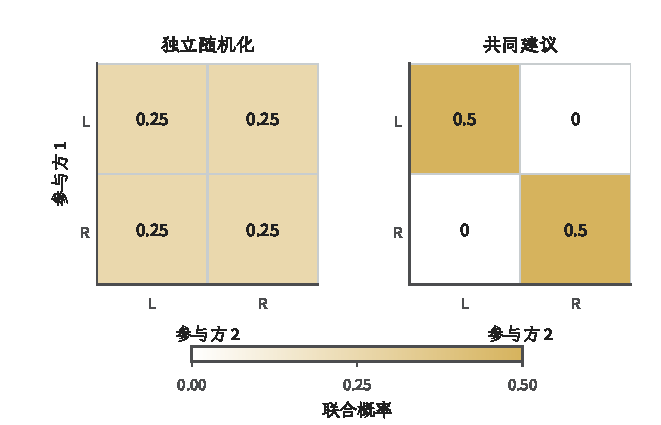
\includegraphics[width=\linewidth]{figures/math-preparation/concept-revision-dynamics/correlated-mass.pdf}
  \caption{二行动协调博弈的两个教学联合分布，共用$0$至$0.5$的概率色阶。
  行为参与者1的行动，列为参与者2的行动。左图为独立均匀策略，四格质量均为$0.25$；
  右图只推荐$(L,L)$与$(R,R)$，各占$0.5$。两者边缘概率均为$(0.5,0.5)$，
  但每人期望收益分别为$1$和$2$；相关分布并非边缘分布的乘积。}
  \label{fig:game-correlated-mass}
\end{figure}

\begin{table}[htbp]
  \centering
  \begin{tabular}{lcc}
    \toprule
    联合行动 & 独立混合概率 & 共同推荐概率\\
    \midrule
    $(L,L)$ & $1/4$ & $1/2$\\
    $(L,R)$ & $1/4$ & $0$\\
    $(R,L)$ & $1/4$ & $0$\\
    $(R,R)$ & $1/4$ & $1/2$\\
    \midrule
    每人的期望收益 & $1$ & $2$\\
    \bottomrule
  \end{tabular}
  \caption{同一边缘分布下的不同联合行动规律。教学协调博弈在相同行动时各得$2$，
  不同时各得$0$。右列是相关均衡，左列是独立混合Nash均衡；收益比较只针对这两个
  分布，纯策略协调均衡同样可以达到收益$2$。}
  \label{tab:game-independent-correlated-actions}
\end{table}

\section{按行动时可用的信息限制完整策略}
\label{sec:game-extensive-information}

收益矩阵将一套完整计划视为一个行动，但隐藏了行动顺序与当时可用的信息。
对三张牌博弈，看到自己牌面后的行动和看到对手质询后的行动不能依赖同一信息。
历史树记录先后关系，信息集把参与者无法区分的历史放在一起，从而限定策略能怎样实施。
这种信息限制独立于零和或一般和的收益分类，也决定下一节允许比较哪些策略偏离。

\subsection{历史树、机会节点与信息集}

\begin{definition}[有限扩展式博弈的历史树]
\label{def:game-finite-extensive-history}
\term{扩展式博弈}（extensive-form game）用历史树保留这些信息。记\(H\)为非空有限历史
集合，空历史为\(\varnothing\)。它满足前缀封闭：若一串行动属于\(H\)，删去末尾
若干行动所得的前缀仍属于\(H\)。不能再延长的历史组成终止集合\(Z\subset H\)。
若\(h\notin Z\)，可选行动集合\(A(h)\)规定合法后继\(ha\)，参与者函数\(P(h)\)
指出下一步由哪位参与者行动；机会节点记为\(P(h)=c\)，其行动概率
\(\sigma_c(a\mid h)\)已给定、非负且在\(A(h)\)上和为\(1\)。终止历史\(z\)为每位
参与者给出收益\(u_i(z)\)。对各参与者，还需指定下面的信息集划分，才能完整确定博弈。
\end{definition}

三张牌质询博弈的机会节点先选择\(H\)或\(L\)，概率各为\(1/2\)。参与者1看到牌面，
所以“拿到\(H\)”与“拿到\(L\)”属于两个不同决策位置。若他选择\(P\)，历史立即
终止；若选择\(B\)，参与者2行动。参与者2只看到“发生了质询”，无法区分历史
\((H,B)\)与\((L,B)\)。

对参与者\(i\)，记全部由其行动的非终止历史为
\[
  H_i=\{h\in H\setminus Z:P(h)=i\}.
\]
\begin{definition}[信息集]
\label{def:game-information-set}
参与者\(i\)的\term{信息集}（information set）族\(\mathcal{I}_i\)是\(H_i\)
的一个划分，每个信息集\(I\in\mathcal{I}_i\)收集参与者当时无法区分的决策历史。
同一信息集中的历史必须具有相同的合法行动集，记这个共同集合为
\(A(I)=A(h)\)，其中\(h\in I\)。
\end{definition}
否则参与者连“现在能做什么”都无法由观察确定。
牌面例子中，参与者2的信息集为
\[
  I_2=\{(H,B),(L,B)\},
\]
可选行动都是\(\{C,F\}\)。信息集不是状态的另一名称。第
~\ref{sec:decision-dynamic-programming}节中的Markov状态用于预测给定行动后的未来
分布；信息集描述当前参与者无法区分哪些历史。两个节点可以有相同物理状态，却因参与者
记得不同过去而属于不同信息集，也可以物理状态不同却因观察受限而位于同一信息集。
参与者\(i\)的纯策略必须为每个\(I\in\mathcal{I}_i\)指定一个
\(A(I)\)中的行动，包括均衡路径上不会到达的信息集；因此它是一份完整的应急计划，
而不只是实际走过路径上的动作序列。

表~\ref{tab:game-card-information}将同一个小博弈中“真实发生了什么”和“行动者
能区分什么”并列写出。参与者2在两条质询历史上必须用同一个$c$，因为他看到的数据
相同。若直接为高牌和低牌分别设置$c_H,c_L$，便改变了可用信息，得到另一个博弈，
即使收益函数没有改动也不能复用当前的均衡。

\begin{table*}[htbp]
  \centering
  \begin{tabularx}{\linewidth}{lXXX}
    \toprule
    行动者 & 真实决策历史 & 当时可区分的信息 & 合法行动规则\\
    \midrule
    参与者1 & 拿到$H$或拿到$L$ & 私人牌面可见，属于两个信息集 & 可分别选$b_H,b_L$\\
    参与者2 & $(H,B)$或$(L,B)$ & 只看到质询，属于同一信息集 & 两条历史共用应对概率$c$\\
    机会 & 初始发牌 & 已给定的环境随机化 & $P(H)=P(L)=1/2$，参与者不能选择\\
    \bottomrule
  \end{tabularx}
  \caption{三张牌教学博弈的信息约束。$b_H,b_L$为对应牌面上的质询概率，$c$为
  参与者2看到质询后的应对概率。这些行为策略记号将在下一小节正式使用。}
  \label{tab:game-card-information}
\end{table*}

\subsection{行为策略、混合策略与完全回忆}

\begin{definition}[行为策略]
\label{def:game-behavior-strategy}
参与者\(i\)的\term{行为策略}（behavior strategy）
\(\sigma_i(a\mid I)\)在每个信息集\(I\in\mathcal{I}_i\)上分别给出$A(I)$上的概率分布；
同一信息集中的所有历史必须使用同一分布。
\end{definition}
三张牌例子可写成三个数：
\[
  b_H=\sigma_1(B\mid I_H),\qquad
  b_L=\sigma_1(B\mid I_L),\qquad
  c=\sigma_2(C\mid I_2).
\]
第~\ref{sec:game-matrix-zero-sum-duality}节得到的均衡对应
\[
  b_H^\star=1,\qquad b_L^\star=\frac13,\qquad c^\star=\frac13.
\]

战略式中的混合策略是在游戏开始时随机抽取一个完整纯计划；行为策略则在每个信息集
到达时随机选择。二者在一般情形下并不等价。若参与者会忘记自己早先知道的牌或采取的
行动，开局抽取的同一个随机计划可以在多个时刻制造相关性，而独立的局部随机化未必能
复制这种相关性。

\begin{definition}[完全回忆]
\label{def:game-perfect-recall}
\term{完全回忆}（perfect recall）要求参与者在同一信息集内不能混淆自己过去获得的
信息和采取的行动。更具体地说，任意两个属于同一信息集的历史，沿途经过的该参与者
信息集序列及其本人行动序列必须相同；这里的过去序列只记录当前节点之前的本人决策。
\end{definition}

\begin{theorem}[Kuhn实现等价]
\label{thm:game-kuhn-equivalence}
在有限完全回忆扩展式博弈中，对任一参与者，任意混合策略都存在一个行为策略，使二者
面对任意固定的对手与机会策略时诱导相同的终止历史分布；任意行为策略也存在具有同样
性质的混合策略。
\end{theorem}

\begin{proof}
先从混合策略构造行为策略。设\(\mu_i\)是在有限纯策略集合上的分布。完全回忆保证
每个信息集\(I\)都有唯一的本人前缀
\[
  \rho_i(I)
  =
  \bigl((I_1,a_1),\ldots,(I_k,a_k)\bigr),
\]
即到达\(I\)以前本人依次经过的信息集和采取的行动；同一\(I\)中的所有历史共享这条
前缀。记\(E_I\)为纯策略与这条前缀一致的事件。若
\(\mu_i(E_I)>0\)，定义
\[
  \sigma_i(a\mid I)
  =
  \frac{
    \mu_i\bigl(E_I\cap\{s_i:s_i(I)=a\}\bigr)
  }{
    \mu_i(E_I)
  },
\]
其中\(s_i\)表示一项完整纯策略，事件\(s_i(I)=a\)表示它在当前信息集指定行动
\(a\)；若分母为零，
就在\(A(I)\)上任取一个分布。

沿任意终止历史依次考察参与者\(i\)的行动。链式法则表明，\(\mu_i\)抽取的完整计划
与这条本人行动序列一致的概率，等于上述各条件概率的乘积，也就是行为策略
\(\sigma_i\)沿该历史贡献的到达概率。对手与机会的路径概率在两种表示下相同，所以
每个终止历史的总概率相同。分母为零的信息集只位于\(\mu_i\)赋予零概率的本人前缀
之后，任意补全都不改变这一结论。

反过来，给定行为策略\(\sigma_i\)，在游戏开始前为每个信息集独立抽取一个行动，并
把全部抽取结果组成纯策略\(s_i\)。令
\[
  \mu_i(s_i)
  =
  \prod_{I\in\mathcal{I}_i}
  \sigma_i\bigl(s_i(I)\mid I\bigr).
\]
对任意终止历史，把未出现在该历史上的信息集行动求和后都得到因子\(1\)，剩余因子
恰是行为策略沿该历史的行动概率乘积。因此该混合策略面对任意对手与机会策略，也诱导
与原行为策略相同的终止历史分布。
\end{proof}

完全回忆不能省略。考虑一位参与者先在\(I_1\)选择\(L\)或\(R\)，随后到达同一个
信息集\(I_2\)，却忘记了刚才的选择，并在\(I_2\)选择\(l\)或\(r\)。混合策略可以
各以\(1/2\)抽取完整计划\((L,l)\)与\((R,r)\)，只产生\(Ll\)和\(Rr\)两条历史。
任何行为策略若让第一步的\(L,R\)都以正概率出现，且让第二步的\(l,r\)也都以正概率
出现，就还会以正概率产生\(Lr\)和\(Rl\)；若把某个概率设为零，又无法同时保留前两条
历史各\(1/2\)的概率。因此局部独立随机化不能复现混合计划中的跨时相关性。

牌面例子满足完全回忆。参与者1只行动一次，参与者2也只在一个信息集行动，不存在忘记
自身观察或动作的机会。矩阵混合
\((B,P)\)概率\(2/3\)、\((B,B)\)概率\(1/3\)，在高牌信息集总是选择\(B\)，在
低牌信息集以概率\(1/3\)选择\(B\)，正好得到上述行为策略。

\subsection{自身、对手与机会到达概率}

给定联合行为策略\(\bm{\sigma}\)，历史
\[
  h=(a_1,\ldots,a_k)
\]
的\term{到达概率}（reach probability）是沿路径各次行动概率之积。把机会也看作
固定策略，可以写成
\begin{equation}
  \pi^{\bm{\sigma}}(h)
  =
  \pi_i^{\bm{\sigma}}(h)
  \pi_{-i}^{\bm{\sigma}}(h),
  \label{eq:game-reach-factorization}
\end{equation}
其中\(\pi_i^{\bm{\sigma}}(h)\)只乘参与者\(i\)在路径上的行动概率，
\(\pi_{-i}^{\bm{\sigma}}(h)\)则乘其他参与者与机会的概率。这个分解不会声称两部分
随机变量独立；它只是把同一条路径上的乘积按行动者归组。

从历史\(h\)继续到终止历史\(z\)的条件路径概率记为
\(\pi^{\bm{\sigma}}(h,z)\)。
\begin{definition}[反事实价值]
\label{def:game-counterfactual-value}
给定上述联合行为策略及到达权重，参与者\(i\)在信息集\(I\)采取行动\(a\in A(I)\)的
\term{反事实价值}（counterfactual value）定义为
\begin{equation}
  v_i^{\bm{\sigma}}(I,a)
  =
  \sum_{h\in I}
  \pi_{-i}^{\bm{\sigma}}(h)
  \sum_{z\succeq ha}
  \pi^{\bm{\sigma}}(ha,z)u_i(z).
  \label{eq:game-counterfactual-action-value}
\end{equation}
信息集当前策略的反事实价值为
\begin{equation}
  v_i^{\bm{\sigma}}(I)
  =
  \sum_{a\in A(I)}
  \sigma_i(a\mid I)
  v_i^{\bm{\sigma}}(I,a).
  \label{eq:game-counterfactual-value}
\end{equation}

\end{definition}
式~\eqref{eq:game-counterfactual-action-value}保留对手和机会到达\(I\)的权重，
却去掉参与者\(i\)自己在到达\(I\)以前的概率。它在问：假设参与者\(i\)把自己送到
这个信息集，其他方和机会以当前方式到达各节点时，当前行动价值如何。去掉自身到达权重
使一个很少被当前自身策略访问的信息集仍能积累学习信号。

在均衡牌面策略下，参与者2的信息集包含高牌质询与低牌质询两个节点。对参与者2而言，
相应反事实到达权重为
\[
  \frac12 b_H^\star=\frac12,
  \qquad
  \frac12 b_L^\star=\frac16.
\]
若把它们归一化，得到到达信息集后的信念
\[
  \mathbb{P}(H\mid B)=\frac34,\qquad
  \mathbb{P}(L\mid B)=\frac14.
\]
在这组权重下，参与者2选择应对的反事实价值为
$\frac12(-2)+\frac16(2)=-\frac23$，退让的反事实价值为
$(\frac12+\frac16)(-1)=-\frac23$。除以总权重$2/3$后，两项条件期望收益都为$-1$。
局部是否偏好一个行动由同一比例缩放保持，但跨信息集求和必须保留原权重。
后验概率用于该信息集内的条件决策，反事实价值则保留未归一化权重，以便把不同信息集的
局部偏离加回整局收益。两者只差一个到达概率因子，却服务于不同推导。

\subsection{信息结构与策略可实施性}

参与者2不能规定“看到高牌质询时应对，看到低牌质询时退让”，因为两个历史位于同一
信息集。一个策略偏离必须对信息集中的所有节点采用同一行动分布。若额外公开牌面，
\(I_2\)会拆成两个单点信息集，允许偏离集合扩大，原均衡也随之改变。信息增加不只是
改善概率估计，它还改变可实施策略的定义域。

未以正概率到达的信息集会带来信念边界。Nash均衡检查完整策略中的单方偏离，但不要求
每个零概率信息集上的信念都由Bayes公式唯一决定。若要分析序贯理性，需要进一步规定
扰动、信念一致性或更精细的均衡概念。本章只保留后续遗憾分解所需的完全回忆和到达概率，
不把Nash存在性扩写成所有动态精炼结论。

这里的“反事实”也不同于第~\ref{chap:causal-inference}章的因果反事实。因果反事实
固定同一单位的外生背景，再替换结构方程中的行动；反事实价值则人为去掉某位参与者的
自身到达概率，以衡量信息集上的策略偏离。两者都讨论“没有实际发生的另一选择”，但
概率空间、固定对象和识别问题并不相同。

\section{用局部遗憾控制整局偏离与平均策略}
\label{sec:game-regret-cfr}

前面已明确可实施策略和允许偏离，均衡存在却没有给出参与者怎样学习策略。
遗憾把实际多轮收益与某个替代策略的收益比较，是对学习过程的评价。
先在普通行动集上建立累计界，再借助信息集和完全回忆分解扩展式博弈的偏离；
得到平均策略的保证时，仍要区分它与末次策略收敛。

\subsection{外部遗憾、内部遗憾与比较类}

\begin{definition}[外部遗憾]
\label{def:game-external-regret}
设行动集$A$非空且有限，同一参与者连续进行\(T\)轮决策。第\(t\)轮选择行动\(a_t\)，并面对损失函数
\(\ell_t:A\to\mathbb{R}\)。相对于事后最佳固定行动的
\term{外部遗憾}（external regret）为
\begin{equation}
  R_{\mathrm{ext}}^T
  =
  \max_{a\in A}
  \sum_{t=1}^{T}
  \bigl(\ell_t(a_t)-\ell_t(a)\bigr).
  \label{eq:game-external-regret}
\end{equation}
\end{definition}
若\(R_{\mathrm{ext}}^T/T\to0\)，平均每轮损失渐近不高于任何一个始终使用的固定
行动。比较对象不是每轮都知道\(\ell_t\)后重新选择的动态先知；后者通常能取得更小
损失，也需要额外的变化预算或可预测性假设。

\begin{definition}[内部遗憾]
\label{def:game-internal-regret}
在同一行动损失序列下，\term{内部遗憾}（internal regret）允许把每次实际选择\(a\)的轮次统一替换成另一
行动\(b\)：
\[
  R_{a\to b}^T
  =
  \sum_{t=1}^{T}
  \mathbb{I}\{a_t=a\}
  \bigl(\ell_t(a)-\ell_t(b)\bigr).
\]
对$(a,b)\in A\times A$分别计算上述量，最大正部称为该轮数下的内部遗憾。
\end{definition}
所有这类替换的正遗憾都很小，意味着参与者看到“原本要选\(a\)”这一信号后，也不愿
系统地改成\(b\)。这正对应相关均衡中依赖建议的偏离；外部遗憾只对应粗相关均衡中的
固定偏离。

\subsection{投影更新的累计遗憾界}

第~\ref{sec:opt-nonsmooth-proximal}节的投影不只用于离线优化，也能控制在线累计
损失\scite{math-zinkevich2003online}设\(C\subseteq\mathbb{R}^d\)为非空闭凸集，
直径至多为\(D\geq0\)，即对任意\(\bm{u},\bm{v}\in C\)都有
\(\lVert\bm{u}-\bm{v}\rVert_2\leq D\)。给定轮数\(T\geq1\)和步长\(\eta>0\)，
第\(t\)轮在选择
\(\bm{w}^{(t)}\in C\)后观察凸损失\(f_t\)，取次梯度
\(\bm{g}^{(t)}\in\partial f_t(\bm{w}^{(t)})\)，并假设
\(\lVert\bm{g}^{(t)}\rVert_2\leq G\)，其中\(G\geq0\)。在线投影次梯度更新为
\begin{equation}
  \bm{w}^{(t+1)}
  =
  \Pi_C\bigl(
    \bm{w}^{(t)}-\eta\bm{g}^{(t)}
  \bigr).
  \label{eq:game-online-projected-gradient}
\end{equation}

\begin{theorem}[在线投影次梯度的外部遗憾]
\label{thm:game-online-gradient-regret}
对任意比较点\(\bm{w}\in C\)，更新
\eqref{eq:game-online-projected-gradient}满足
\begin{equation}
  \sum_{t=1}^{T}
  \bigl(
    f_t(\bm{w}^{(t)})-f_t(\bm{w})
  \bigr)
  \leq
  \frac{D^2}{2\eta}
  +\frac{\eta G^2T}{2}.
  \label{eq:game-online-gradient-regret-bound}
\end{equation}
当\(D>0\)且\(G>0\)时，取\(\eta=D/(G\sqrt{T})\)，右侧为
\(DG\sqrt{T}\)。若\(D=0\)，则\(C\)只有一个点；若\(G=0\)，次梯度不等式说明
每轮差值都不大于零。两种退化情形的遗憾上界均为零，无需使用这个步长公式。
\end{theorem}

\begin{proof}
欧氏投影不会增加到任意可行点的距离，所以
\begin{align*}
  \lVert\bm{w}^{(t+1)}-\bm{w}\rVert_2^2
  &\leq
  \lVert
    \bm{w}^{(t)}-\eta\bm{g}^{(t)}-\bm{w}
  \rVert_2^2\\
  &=
  \lVert\bm{w}^{(t)}-\bm{w}\rVert_2^2
  -2\eta
  \langle
    \bm{g}^{(t)},\bm{w}^{(t)}-\bm{w}
  \rangle
  +\eta^2\lVert\bm{g}^{(t)}\rVert_2^2.
\end{align*}
凸函数的次梯度不等式给出
\[
  f_t(\bm{w}^{(t)})-f_t(\bm{w})
  \leq
  \langle
    \bm{g}^{(t)},\bm{w}^{(t)}-\bm{w}
  \rangle.
\]
把内积从距离展开式中解出并代入，得到
\[
  f_t(\bm{w}^{(t)})-f_t(\bm{w})
  \leq
  \frac{
    \lVert\bm{w}^{(t)}-\bm{w}\rVert_2^2
    -
    \lVert\bm{w}^{(t+1)}-\bm{w}\rVert_2^2
  }{2\eta}
  +\frac{\eta G^2}{2}.
\]
对\(t\)求和后，距离平方项望远镜消去，只剩初始距离上界\(D^2\)，得到
式~\eqref{eq:game-online-gradient-regret-bound}。当\(D,G>0\)时，对右侧关于
\(\eta\)配平即得\(DG\sqrt{T}\)；退化情形按定理后的说明处理。
\end{proof}

这个证明允许损失序列依赖过去行动，只要当前行动在当前损失揭晓前确定。它给出
\(O(\sqrt{T})\)累计遗憾和\(O(T^{-1/2})\)平均遗憾，却没有声称
\(\bm{w}^{(t)}\)本身收敛。把低遗憾用于博弈时，通常得到经验分布或平均策略的结论。

概率单纯形把这个通用更新接回混合策略。设行动集为
\(A=\{B,P\}\)，取\(C=\Delta(A)\)，并令第\(t\)轮两个行动的损失向量为
\(\bm{\ell}^{(t)}\)。分布\(\bm{w}\in C\)的期望损失
\[
  f_t(\bm{w})
  =
  \langle\bm{w},\bm{\ell}^{(t)}\rangle
\]
是线性函数，次梯度就是\(\bm{\ell}^{(t)}\)。若
\(\bm{w}^{(t)}=(1/2,1/2)^{\top}\)、
\(\bm{\ell}^{(t)}=(0,1)^{\top}\)且\(\eta=1/2\)，则
\[
  \Pi_{\Delta(A)}
  \left(
    \bm{w}^{(t)}-\eta\bm{\ell}^{(t)}
  \right)
  =
  (3/4,1/4)^{\top}.
\]
投影把概率从本轮损失较大的\(P\)移向\(B\)，同时保持坐标非负且和为\(1\)。
定理因而说明混合策略空间上可以构造局部无外部遗憾更新。下面的CFR在各信息集采用
遗憾匹配，而不是必须采用欧氏投影；这里的通用结果用于建立两类更新共享的无遗憾目标。

\subsection{信息集上的即时反事实遗憾}

前两小节采用损失约定，遗憾写成实际损失减替代损失。扩展式博弈沿用收益函数，下面改用
收益约定，把遗憾写成替代收益减当前收益；令损失等于收益的相反数，就能在两种约定之间
转换，正遗憾始终表示偏离更有利。

在第\(t\)轮扩展式博弈中，联合策略记为\(\bm{\sigma}^{(t)}\)。参与者\(i\)在信息集
\(I\)把当前随机行动改成固定行动\(a\)的即时反事实遗憾为
\begin{equation}
  r_i^{(t)}(I,a)
  =
  v_i^{\bm{\sigma}^{(t)}}(I,a)
  -
  v_i^{\bm{\sigma}^{(t)}}(I).
  \label{eq:game-immediate-counterfactual-regret}
\end{equation}
累计量及其正部最大值记为
\[
  R_i^T(I,a)
  =
  \sum_{t=1}^{T}r_i^{(t)}(I,a),
  \qquad
  R_{i,+}^T(I)
  =
  \max\left\{0,\max_{a\in A(I)}R_i^T(I,a)\right\}.
\]

\term{反事实遗憾最小化}（counterfactual regret minimization, CFR）在每个信息集
运行一个局部无遗憾算法\scite{math-zinkevich2007cfr}一次完整树更新包含四步：
固定本轮联合行为策略并遍历历史树，计算各信息集的反事实行动价值；用
式~\eqref{eq:game-immediate-counterfactual-regret}累计每个行动的遗憾；用局部
遗憾匹配生成下一轮策略；同时按本人的到达概率累计平均策略所需的实现权重。这里的
“最小化”是让平均遗憾趋近于零，不是逐轮直接最小化某个静态目标。

典型的\term{遗憾匹配}（regret matching）按正累计遗憾选择下一轮行动：
\begin{equation}
  \sigma_i^{(t+1)}(a\mid I)
  =
  \begin{cases}
    \displaystyle
    \frac{[R_i^t(I,a)]_+}
         {\sum_b[R_i^t(I,b)]_+},
      &\sum_b[R_i^t(I,b)]_+>0,\\[8pt]
    \displaystyle\frac{1}{|A(I)|},
      &\text{否则}.
  \end{cases}
  \label{eq:game-regret-matching}
\end{equation}

若存在\(\Delta_I\geq0\)，使对每轮\(t=1,\ldots,T\)及任意
\(a,b\in A(I)\)都有
\[
  \left|
    v_i^{\bm{\sigma}^{(t)}}(I,a)
    -
    v_i^{\bm{\sigma}^{(t)}}(I,b)
  \right|
  \leq\Delta_I,
\]
则遗憾匹配满足
\begin{equation}
  R_{i,+}^T(I)
  \leq
  \Delta_I\sqrt{|A(I)|T}.
  \label{eq:game-local-regret-matching-bound}
\end{equation}
证明可用势函数
\(\Phi_t=\sum_a[R_i^t(I,a)]_+^2\)。每轮平方展开中的交叉项为
\[
  2\sum_a[R_i^{t-1}(I,a)]_+r_i^{(t)}(I,a).
\]
当正遗憾和非零时，式~\eqref{eq:game-regret-matching}使它正比于
\(\sum_a\sigma_i^{(t)}(a\mid I)r_i^{(t)}(I,a)=0\)；正遗憾和为零时，
交叉项也不为正。平方增量至多
\(\sum_a(r_i^{(t)}(I,a))^2\leq |A(I)|\Delta_I^2\)。
归纳得到
\(\Phi_T\leq T|A(I)|\Delta_I^2\)，而每个正累计遗憾的平方不超过
\(\Phi_T\)，于是得到式~\eqref{eq:game-local-regret-matching-bound}。

\subsection{牌面博弈的反事实遗憾计算}

用三张牌博弈核对一次参与者2的CFR更新。假设当前策略取
\[
  b_H=b_L=\frac12,\qquad
  \sigma_2(C\mid I_2)=\sigma_2(F\mid I_2)=\frac12.
\]
参与者2到达高牌质询节点和低牌质询节点的反事实权重都为
\[
  \frac12\cdot\frac12=\frac14.
\]
第一个因子来自机会发牌，第二个因子来自参与者1质询。应对
\(C\)时，参与者2在高牌和低牌节点的收益分别为\(-2\)与\(2\)，所以
\[
  v_2(I_2,C)
  =
  \frac14(-2)+\frac14(2)=0.
\]
退让\(F\)时，参与者1在两个节点都得到\(1\)，参与者2因而都得到\(-1\)，所以
\[
  v_2(I_2,F)
  =
  \frac14(-1)+\frac14(-1)=-\frac12.
\]
当前均匀策略的反事实价值为\(-1/4\)，本轮即时遗憾因此为
\[
  r_2(I_2,C)=\frac14,\qquad
  r_2(I_2,F)=-\frac14.
\]
若此前累计遗憾为零，遗憾匹配在下一轮把全部概率放到\(C\)。这个结果只描述一次局部
更新；参与者2更常应对以后，低牌质询会变得不利，参与者1的后续更新又会改变两个节点的
权重。因而不能把首轮纯响应当成收敛策略，也不能从这一个数值步骤推出均衡保证。

\subsection{完全回忆与局部遗憾分解}

整局外部遗憾允许参与者把当前行为策略替换成任意固定行为策略：
\begin{equation}
  R_i^T
  =
  \max_{\widetilde{\sigma}_i}
  \sum_{t=1}^{T}
  \left[
    u_i(\widetilde{\sigma}_i,\bm{\sigma}_{-i}^{(t)})
    -
    u_i(\bm{\sigma}^{(t)})
  \right].
  \label{eq:game-extensive-external-regret}
\end{equation}
局部反事实遗憾之所以有用，在于它们能够上界这个看似覆盖整棵树的比较。

\begin{theorem}[CFR的反事实遗憾分解]
\label{thm:game-cfr-decomposition}
在有限完全回忆扩展式博弈中，
\begin{equation}
  R_i^T
  \leq
  \sum_{I\in\mathcal{I}_i}
  R_{i,+}^T(I).
  \label{eq:game-cfr-global-bound}
\end{equation}
\end{theorem}

\begin{proof}
固定替代行为策略\(\widetilde{\sigma}_i\)。证明先在一轮中把整局偏离逐层拆开，再对
轮次求和。为看清拆分发生在哪里，对\(h\in I\)定义当前策略在行动\(a\)后的条件续局
收益
\[
  q_i^{(t)}(h,a)
  =
  \sum_{z\succeq ha}
  \pi^{\bm{\sigma}^{(t)}}(ha,z)u_i(z),
\]
并以\(\widetilde q_i^{(t)}(h,a)\)表示对手和机会仍采用
\(\bm{\sigma}_{-i}^{(t)}\)，而参与者\(i\)从\(ha\)以后采用
\(\widetilde{\sigma}_i\)时的同一数值，即
\[
  \widetilde q_i^{(t)}(h,a)
  =
  \sum_{z\succeq ha}
  \pi^{(\widetilde{\sigma}_i,\bm{\sigma}_{-i}^{(t)})}(ha,z)
  u_i(z).
\]
当前策略从\(h\)出发的续局收益为
\(q_i^{(t)}(h)=\sum_b\sigma_i^{(t)}(b\mid I)q_i^{(t)}(h,b)\)。
在替代收益中加上再减去“只在当前行动改用替代分布、以后仍用当前策略”的收益，逐历史
得到恒等式
\begin{align}
  &\sum_{a\in A(I)}
  \widetilde{\sigma}_i(a\mid I)
  \widetilde q_i^{(t)}(h,a)
  -
  q_i^{(t)}(h)
  \notag\\
  &\quad=
  \sum_{a\in A(I)}
  \widetilde{\sigma}_i(a\mid I)
  \bigl(q_i^{(t)}(h,a)-q_i^{(t)}(h)\bigr)
  \notag\\
  &\qquad\quad+
  \sum_{a\in A(I)}
  \widetilde{\sigma}_i(a\mid I)
  \bigl(
    \widetilde q_i^{(t)}(h,a)-q_i^{(t)}(h,a)
  \bigr).
  \label{eq:game-history-deviation-identity}
\end{align}
第一项只改变当前信息集的行动，第二项只记录当前行动之后继续偏离的收益。

下面把逐历史恒等式汇总到信息集。记
\(\mathcal{C}_i(I,a)\)为采取\(a\)以后、在参与者\(i\)再次行动时首次遇到的本人
信息集集合；若在此之前终止，就没有后继信息集。令
\(\widetilde v_i^{(t)}(I)\)为到达\(I\)的对手与机会权重仍取
\(\pi_{-i}^{\bm{\sigma}^{(t)}}(h)\)，但从\(I\)起参与者\(i\)都采用
\(\widetilde{\sigma}_i\)的反事实价值，并记
\[
  D_i^{(t)}(I)
  =
  \widetilde v_i^{(t)}(I)
  -
  v_i^{\bm{\sigma}^{(t)}}(I),
  \qquad
  L_i^{(t)}(I)
  =
  \sum_a
  \widetilde{\sigma}_i(a\mid I)r_i^{(t)}(I,a).
\]
将式~\eqref{eq:game-history-deviation-identity}乘以
\(\pi_{-i}^{\bm{\sigma}^{(t)}}(h)\)并对\(h\in I\)求和，得到信息集偏离收益恒等式
\begin{equation}
  D_i^{(t)}(I)
  =
  L_i^{(t)}(I)
  +
  \sum_{a\in A(I)}
  \widetilde{\sigma}_i(a\mid I)
  \sum_{I'\in\mathcal{C}_i(I,a)}
  D_i^{(t)}(I').
  \label{eq:game-information-set-deviation-identity}
\end{equation}
这里没有漏掉从\(I\)到\(I'\)之间的概率：这段路径上参与者\(i\)不再行动，对手和
机会的路径概率与\(I\)处已有的权重相乘，正好成为\(I'\)中各历史的
\(\pi_{-i}^{\bm{\sigma}^{(t)}}\)。在遇到下一个本人信息集以前终止的路径上，两种
策略的后续行为相同，故其第二项为零。

完全回忆使本人信息集及边\((I,a)\to I'\)组成一个森林。确切地说，同一信息集
\(I'\)中的所有历史具有相同的本人既往信息集与行动序列，所以每个非根信息集都有唯一的
前驱边；对手或机会的多条历史可以汇入同一个\(I'\)，但这些历史只在
\(\pi_{-i}^{\bm{\sigma}^{(t)}}\)的求和中合并，不会把\(I'\)复制成多个后继。
记\(\widetilde{\pi}_i(I)\)为替代策略沿该唯一本人前缀的行动概率乘积；根信息集的
乘积约定为\(1\)。这正是反事实价值中故意省去的自身到达概率。

现在按一个信息集之后还可能遇到的本人信息集层数归纳。最深信息集没有后继，
式~\eqref{eq:game-information-set-deviation-identity}给出
\(D_i^{(t)}(I)=L_i^{(t)}(I)\)。假设所有深度更小的后继子树都已展开，把它们代回
同一恒等式；由于每个后继只有一个前驱，子树中的每个信息集恰好出现一次，其系数等于
沿唯一前缀的\(\widetilde{\sigma}_i\)行动概率乘积。对森林的所有根求和后便得到
\begin{equation}
  u_i(\widetilde{\sigma}_i,\bm{\sigma}_{-i}^{(t)})
  -
  u_i(\bm{\sigma}^{(t)})
  =
  \sum_{I\in\mathcal{I}_i}
  \widetilde{\pi}_i(I)
  \sum_{a\in A(I)}
  \widetilde{\sigma}_i(a\mid I)r_i^{(t)}(I,a).
  \label{eq:game-global-deviation-identity}
\end{equation}
参与者\(i\)从未行动就终止的历史在两种策略下收益相同，因而不出现在右侧。
式~\eqref{eq:game-global-deviation-identity}明确分开了两类权重：对手与机会的权重
已经包含在\(r_i^{(t)}(I,a)\)中，自身在替代策略下到达\(I\)的权重则是外部系数
\(\widetilde{\pi}_i(I)\)。

替代策略固定后，\(\widetilde{\pi}_i(I)\)和
\(\widetilde{\sigma}_i(a\mid I)\)都不随\(t\)变化。对
式~\eqref{eq:game-global-deviation-identity}求和，并使用
\(0\leq\widetilde{\pi}_i(I)\leq1\)，可得
\begin{align*}
  &\sum_{t=1}^{T}
  \left[
    u_i(\widetilde{\sigma}_i,\bm{\sigma}_{-i}^{(t)})
    -
    u_i(\bm{\sigma}^{(t)})
  \right]\\
  &\quad=
  \sum_I
  \widetilde{\pi}_i(I)
  \sum_a
  \widetilde{\sigma}_i(a\mid I)R_i^T(I,a)\\
  &\quad\leq
  \sum_I
  \widetilde{\pi}_i(I)
  \max_a R_i^T(I,a)
  \leq
  \sum_I R_{i,+}^T(I).
\end{align*}
最后一个不等式也覆盖\(\max_aR_i^T(I,a)<0\)的情形，因为此时相应正部为零。
右侧与替代策略无关，再对\(\widetilde{\sigma}_i\)取最大，就得到
式~\eqref{eq:game-cfr-global-bound}。
\end{proof}

若缺少完全回忆，同一当前信息集可能汇合不同的本人行动历史。此时局部策略无法知道应该
补回哪条自身到达路径，上述递归可能重复计算或遗漏偏离收益，局部低遗憾便不再自动控制
整局外部遗憾。

结合式~\eqref{eq:game-local-regret-matching-bound}，CFR得到
\begin{equation}
  R_i^T
  \leq
  \sum_{I\in\mathcal{I}_i}
  \Delta_I\sqrt{|A(I)|T}.
  \label{eq:game-cfr-rate}
\end{equation}
当信息集和行动数固定时，平均外部遗憾按\(O(T^{-1/2})\)趋于零。

\subsection{平均策略的权重与零和保证}

行为策略不能在每个信息集直接做普通算术平均。某轮中一个信息集若几乎不会被参与者自己
到达，该处局部概率不应与频繁到达轮次具有同样权重。完全回忆保证同一信息集
\(I\)中的历史具有同一条本人行动前缀，因而
\(\pi_i^{\bm{\sigma}^{(t)}}(I)\)定义为这条前缀上的本人行动概率乘积，与选取
哪个\(h\in I\)无关。记第\(t\)轮在本人序列\((I,a)\)上的实现权重为
\[
  x_i^{(t)}(I,a)
  =
  \pi_i^{\bm{\sigma}^{(t)}}(I)
  \sigma_i^{(t)}(a\mid I),
\]
并令
\(\overline{x}_i^T(I,a)=T^{-1}\sum_t x_i^{(t)}(I,a)\)以及
\(\overline{x}_i^T(I)=T^{-1}\sum_t
\pi_i^{\bm{\sigma}^{(t)}}(I)\)。CFR使用
\begin{equation}
  \overline{\sigma}_i^T(a\mid I)
  =
  \frac{
    \sum_{t=1}^{T}
    \pi_i^{\bm{\sigma}^{(t)}}(I)
    \sigma_i^{(t)}(a\mid I)
  }{
    \sum_{t=1}^{T}
    \pi_i^{\bm{\sigma}^{(t)}}(I)
  },
  \label{eq:game-cfr-average-strategy}
\end{equation}
其中分母为零时可以任意指定。式~\eqref{eq:game-cfr-average-strategy}等价于
\[
  \overline{\sigma}_i^T(a\mid I)
  =
  \frac{\overline{x}_i^T(I,a)}{\overline{x}_i^T(I)}.
\]

这个权重不是经验修正，而是实现计划平均所要求的条件概率。根本人序列的实现权重为
\(1\)。若\(I\)的唯一本人前驱序列终止于\((J,b)\)，则每一轮都有
\(\pi_i^{\bm{\sigma}^{(t)}}(I)=x_i^{(t)}(J,b)\)，对轮次平均后仍有
\(\overline{x}_i^T(I)=\overline{x}_i^T(J,b)\)。从根序列归纳，并在每个信息集应用
上面的条件概率公式，得到
\begin{equation}
  \pi_i^{\overline{\sigma}_i^T}(I)
  \overline{\sigma}_i^T(a\mid I)
  =
  \overline{x}_i^T(I,a)
  =
  \frac{1}{T}\sum_{t=1}^{T}x_i^{(t)}(I,a).
  \label{eq:game-average-realization-plan}
\end{equation}
因此，加权平均行为策略实现的正是各轮本人实现计划的算术平均。分母为零意味着所有轮次
到达该本人序列的概率都为零，此处怎样指定局部策略都不改变平均实现计划。

在两人零和博弈中，若双方平均外部遗憾分别不超过
\(\varepsilon_1T\)与\(\varepsilon_2T\)，则平均策略满足
\begin{equation}
  \max_{\sigma_1}
  u_1(\sigma_1,\overline{\sigma}_2^T)
  -
  \min_{\sigma_2}
  u_1(\overline{\sigma}_1^T,\sigma_2)
  \leq
  \varepsilon_1+\varepsilon_2.
  \label{eq:game-average-exploitability}
\end{equation}
下面补出这个界。记第\(t\)轮第1位参与者的收益为
\(u_1(\sigma_1^{(t)},\sigma_2^{(t)})\)，并令
\[
  \widehat u_T
  =
  \frac{1}{T}
  \sum_{t=1}^{T}
  u_1(\sigma_1^{(t)},\sigma_2^{(t)}).
\]
终止历史\(z\)的概率可以写成机会概率与双方实现权重之积，所以期望收益对双方实现计划
分别线性。结合式~\eqref{eq:game-average-realization-plan}，对任意固定策略
\(\sigma_1,\sigma_2\)有
\begin{align}
  \frac{1}{T}\sum_{t=1}^{T}
  u_1(\sigma_1,\sigma_2^{(t)})
  &=
  u_1(\sigma_1,\overline{\sigma}_2^T),
  \notag\\
  \frac{1}{T}\sum_{t=1}^{T}
  u_1(\sigma_1^{(t)},\sigma_2)
  &=
  u_1(\overline{\sigma}_1^T,\sigma_2).
  \label{eq:game-average-payoff-linearity}
\end{align}

第1位参与者的外部遗憾界除以\(T\)，再用第一条等式，得到
\begin{equation}
  \max_{\sigma_1}
  u_1(\sigma_1,\overline{\sigma}_2^T)
  -
  \widehat u_T
  \leq
  \varepsilon_1.
  \label{eq:game-row-average-regret}
\end{equation}
第2位参与者的收益为\(u_2=-u_1\)。把其外部遗憾界同样除以\(T\)，并用
式~\eqref{eq:game-average-payoff-linearity}的第二条等式，得到
\begin{equation}
  \widehat u_T
  -
  \min_{\sigma_2}
  u_1(\overline{\sigma}_1^T,\sigma_2)
  \leq
  \varepsilon_2.
  \label{eq:game-column-average-regret}
\end{equation}
将式~\eqref{eq:game-row-average-regret}与
\eqref{eq:game-column-average-regret}相加，经验对局收益
\(\widehat u_T\)消去，正好得到
式~\eqref{eq:game-average-exploitability}。若博弈值为\(v^\star\)，其左侧还可写成
\[
  \left[
    \max_{\sigma_1}u_1(\sigma_1,\overline{\sigma}_2^T)-v^\star
  \right]
  +
  \left[
    v^\star-\min_{\sigma_2}u_1(\overline{\sigma}_1^T,\sigma_2)
  \right].
\]
两项分别衡量第2位和第1位参与者的平均策略可被最佳响应利用多少，且都非负；因此该和是
双方平均策略的零和鞍点间隙。本章把这个和称为\term{联合可利用度}
（joint exploitability）；若采用两项平均的口径，数值还需除以\(2\)。间隙为零时，
两者构成极小极大策略对。

式~\eqref{eq:game-average-exploitability}保证的是两人零和博弈的平均策略，不是最后
一次迭代。一般和博弈中，低外部遗憾使经验联合分布趋近CCE，却不保证平均边缘策略构成
Nash均衡。为看清这里保留的是哪种分布，令第\(t\)轮实际联合行动为
\(\bm{a}^{(t)}\)，经验分布为
\[
  \widehat{\mu}_T(\bm{a})
  =
  \frac{1}{T}
  \sum_{t=1}^{T}
  \mathbb{I}\{\bm{a}^{(t)}=\bm{a}\}.
\]
若参与者\(i\)的平均外部收益遗憾至多\(\varepsilon_i\)，则对任意固定行动
\(a_i'\)，
\[
  \mathbb{E}_{\bm{A}\sim\widehat{\mu}_T}[u_i(\bm{A})]
  \geq
  \mathbb{E}_{\bm{A}\sim\widehat{\mu}_T}
  [u_i(a_i',\bm{A}_{-i})]
  -\varepsilon_i.
\]
这正是带\(\varepsilon_i\)松弛的CCE不等式。若每个有向替换
\(a_i\to b_i\)的平均内部遗憾都不超过\(\varepsilon_i\)，则对任意映射
\(\phi_i\)，把发生\(A_i=a_i\)的轮次按\(a_i\)分组并求和，可得CE偏离收益至多
\(|A_i|\varepsilon_i\)；若直接控制所有映射的交换遗憾，则松弛就是
\(\varepsilon_i\)。这两个结论保留的是联合经验分布中的相关性，不能用各自经验边缘
的乘积替代。

末次策略还可能持续循环。采样CFR若只访问部分历史，还要用第
\ref{chap:stochastic-processes-and-approximation}章的无偏估计、方差和集中工具控制
采样误差，不能把完整树上的确定性分解直接当作有限样本保证。

回到三张牌例子，参与者2的信息集使用高牌质询权重\(1/2\)和低牌质询权重\(1/6\)
计算局部应对遗憾。若算法长期发现应对比退让更好，就提高\(C\)的概率；这一变化又会
降低低牌质询的收益，使参与者1减少虚张声势。双方局部更新相互改变下一轮价值，CFR保证
累计偏离受控，却不要求这两个概率逐轮单调走向\(1/3\)。

把平均遗憾转成均衡结论时，还要保留产生平均的联合样本。
表~\ref{tab:game-regret-comparison-conclusions}比较两种偏离：固定行动只提出一个
事前替代选择，内部替换可以对某种已采取行动单独修改，因此后者需要控制更多比较。
这里的保证针对经验联合分布或相应的平均策略，不对最后一轮作同样承诺。

\begin{table*}[htbp]
  \centering
  \begin{tabularx}{\linewidth}{lXXX}
    \toprule
    偏离比较 & 允许怎样改变 & 一般和下的平均结论 & 两人零和的补充\\
    \midrule
    外部遗憾 & 所有轮次统一改用一个固定行动 & 经验联合分布的粗相关偏离收益小 & 双方平均策略的鞍点差距小\\
    内部遗憾 & 将某种已选行动统一换成另一行动 & 经验联合分布的相关偏离收益小 & 仍需按具体信息结构恢复策略\\
    \bottomrule
  \end{tabularx}
  \caption{遗憾的比较类与平均结论。表中要求每位参与者都控制相应的平均遗憾；
  扩展式博弈的平均行为策略还须使用自身到达权重。末次策略收敛不由这些平均结论推出。}
  \label{tab:game-regret-comparison-conclusions}
\end{table*}

\section{按贡献、退出条件与联盟稳定性分配收益}
\label{sec:game-credit-allocation-multiparty-payoffs}

遗憾与均衡研究参与者各自选择策略。若任务改为合作，并已给出每个联盟能够取得的价值，
问题就变成共同收益怎样分配。边际贡献取决于加入顺序，Shapley值对这些顺序作平均；
联盟是否愿意保持合作则是另一个稳定性要求，需要与分配公平的公理分别核对。

\subsection{联盟价值、边际贡献与分配}

前四节把参与者的收益函数视为已给定对象。合作问题进一步询问：若若干参与者共享信息、
模型或资源并产生共同收益，这个收益应怎样分配？本节所说的
\term{多方信用分配}（multi-party credit allocation），是根据各个联盟能够取得的
价值，为每位参与者确定贡献份额\(\psi_i(v)\)。若还要求预算平衡，则这些份额满足
\(\sum_i\psi_i(v)=v(N)\)。它分配的是参与者对联盟价值的贡献，不是把一条轨迹的
延迟奖励传回各时间步；后者将在强化学习部分作为时序信用分配问题讨论。

\begin{definition}[可转移效用博弈]
\label{def:game-transferable-utility-cooperation}
\term{可转移效用合作博弈}
（transferable-utility cooperative game）由参与者集合\(N\)和联盟价值函数
\[
  v:2^N\to\mathbb{R},\qquad v(\varnothing)=0
\]
组成，$N$为非空有限集合。\(v(S)\)表示联盟\(S\)独立合作时可取得并能在成员之间转移的总收益。
\end{definition}

联盟价值不是从单个模型输出自动得到的。对牌面判断任务，可以把\(v(S)\)定义为联盟
\(S\)共享信号后，相对于无信号基线减少的最优期望损失；也可以定义为收入、正确判断数
或节省的核验成本。不同定义会产生不同分配。若参与者的收益不能用同一尺度转移，例如
一方关心隐私、另一方关心延迟，就需要非可转移效用模型，不能先相加再假装总量可任意
拆分。

参与者\(i\)加入已有联盟\(S\subseteq N\setminus\{i\}\)的边际贡献为
\[
  v(S\cup\{i\})-v(S).
\]
它依赖先到者集合\(S\)。两位牌面观察者可能各自只能提供模糊线索，合在一起却能确定
牌面；此时任何一人的“独立贡献”都不能由单独使用他的信号一次决定。

\subsection{Shapley值与参与顺序平均}

\term{Shapley值}（Shapley value）把参与者在所有随机加入次序中的边际贡献取平均
\scite{math-shapley1953value}
\begin{definition}[Shapley值]
\label{def:game-shapley-value}
对上述可转移效用博弈、\(n=|N|\)及参与者$i\in N$，其Shapley分配为
\begin{equation}
  \phi_i(v)
  =
  \sum_{S\subseteq N\setminus\{i\}}
  \frac{|S|!(n-|S|-1)!}{n!}
  \bigl[
    v(S\cup\{i\})-v(S)
  \bigr].
  \label{eq:game-shapley-value}
\end{equation}
\end{definition}
系数是随机排列中恰好由\(S\)排在\(i\)之前的概率：\(S\)内部有\(|S|!\)种次序，
其余参与者在\(i\)之后有\((n-|S|-1)!\)种次序，总排列数为\(n!\)。

Shapley值满足四项要求。若两位参与者对所有不含二者的联盟产生相同边际贡献，
\term{对称性}要求二者分配相同；若参与者对任意联盟的边际贡献都为零，
\term{虚设参与者性质}要求其分配为零；\term{有效性}要求
\(\sum_i\phi_i(v)=v(N)\)；\term{可加性}要求对两个价值函数
\(v,w\)，有\(\phi_i(v+w)=\phi_i(v)+\phi_i(w)\)。

\begin{theorem}[Shapley值的公理刻画]
\label{thm:game-shapley-characterization}
在有限可转移效用合作博弈上，同时满足对称性、虚设参与者性质、有效性和可加性的分配
规则唯一，并由式~\eqref{eq:game-shapley-value}给出。
\end{theorem}

\begin{proof}
先验证式~\eqref{eq:game-shapley-value}满足四项性质。它是随机排列下边际贡献的期望。
每个排列中，所有参与者的边际贡献沿加入次序望远镜相加为
\[
  v(N)-v(\varnothing)=v(N),
\]
取期望得到有效性。交换两位对称参与者不会改变排列分布或边际贡献分布，得到对称性。
虚设参与者的每项边际贡献都为零。边际贡献关于价值函数线性，取期望后得到可加性。

再证唯一性。设\(\Phi\)是任意满足四项公理的分配规则。对每个非空集合
\(T\subseteq N\)，定义一致联盟博弈
\[
  u_T(S)
  =
  \begin{cases}
    1,&T\subseteq S,\\
    0,&T\nsubseteq S.
  \end{cases}
\]
任意满足\(v(\varnothing)=0\)的价值函数都能唯一写成
\begin{equation}
  v
  =
  \sum_{\varnothing\neq T\subseteq N}
  c_Tu_T,
  \qquad
  c_T
  =
  \sum_{R\subseteq T}
  (-1)^{|T|-|R|}v(R),
  \label{eq:game-unanimity-basis}
\end{equation}
这是子集格上的包含--排除展开。

还要处理展开式中的任意实系数，不能只由重复相加得到整数或有理数倍。对任意
\(c\in\mathbb{R}\)，在博弈\(c\,u_T\)中，\(T\)外的参与者都是虚设参与者，分配
必须为零；\(T\)内参与者彼此对称，有效性又要求他们的分配和为\(c\)，所以每人只能
得到\(c/|T|\)。这个结论直接覆盖正、负及无理的\(c\)，没有预先假设分配规则连续。

式~\eqref{eq:game-unanimity-basis}只有有限项。可加性因此给出
\[
  \Phi(v)
  =
  \sum_{\varnothing\neq T\subseteq N}
  \Phi(c_Tu_T),
\]
而每一项已经由上一段唯一确定，故任意\(v\)上的分配也唯一。特别地，对任意
\(\alpha\in\mathbb{R}\)，对\(\alpha v\)使用同一展开便得到
\(\Phi(\alpha v)=\alpha\Phi(v)\)，这补出了实齐次性。前半部分已经证明
式~\eqref{eq:game-shapley-value}满足这些公理，故它就是唯一规则。
\end{proof}

\subsection{三方信息合作的贡献分配}

把牌面任务扩展为三位信息提供者。参与者1观察牌背纹理，参与者2观察发牌动作，
参与者3提供一次较弱的设备校验。以“相对于无信息基线减少的期望损失”为统一收益单位，
假设教学构造的联盟价值为
\[
\begin{array}{c@{\quad}cccccccc}
  S
  &\varnothing&\{1\}&\{2\}&\{3\}
  &\{1,2\}&\{1,3\}&\{2,3\}&\{1,2,3\}\\ \hline
  v(S)
  &0&1&1&0&3&2&2&4
\end{array}
\]
这些数值只用于展示互补贡献：前两位各自有用，二者合并额外增益较大；第三位单独无用，
却能校验已有线索。

对参与者1，四类前驱联盟的贡献给出
\begin{align*}
  \phi_1(v)
  &=
  \frac13(1-0)
  +\frac16(3-1)
  +\frac16(2-0)
  +\frac13(4-2)\\
  &=\frac53.
\end{align*}
对称性给出\(\phi_2(v)=5/3\)。参与者3的分配为
\begin{align*}
  \phi_3(v)
  &=
  \frac13(0-0)
  +\frac16(2-1)
  +\frac16(2-1)
  +\frac13(4-3)\\
  &=\frac23.
\end{align*}
三者之和为\(4=v(N)\)，与有效性一致。参与者3虽然单独价值为零，却不是虚设参与者，
因为加入\(\{1\}\)、\(\{2\}\)或\(\{1,2\}\)都会增加联盟价值。只按单人表现分配会
漏掉这种互补性。

若把价值改成模型预测分数，Shapley公式仍可计算，但解释也随之改变。它分配的是所定义
价值函数相对于基线的差，不自动等于真实因果贡献。特征彼此相关时，“缺少某个特征”的
联盟输入怎样构造还需要条件分布、边缘分布或干预语义；这些选择分别回答预测归因与因果
效应问题，不能只用同一个Shapley名称消除差异。

\subsection{联盟稳定性、Pareto权衡与协商解}

一个有效分配仍可能被某个联盟拒绝。若分配向量为\(\bm{x}\)，并满足
\[
  \sum_{i\in N}x_i=v(N),
\]
但存在联盟\(S\)使
\[
  \sum_{i\in S}x_i<v(S),
\]
那么该联盟单独合作可取得更多总收益。要求所有联盟都没有这种阻挡，并保持总收益完全
分配，得到一种对所有联盟的稳定性要求。
\begin{definition}[合作博弈的核心]
\label{def:game-cooperative-core}
对可转移效用博弈$(N,v)$，其\term{核心}（core）为分配向量$\bm x\in\mathbb R^{|N|}$的集合，
其中$\sum_{i\in N}x_i=v(N)$，并且$\sum_{i\in S}x_i\geq v(S)$对每个$S\subseteq N$成立。
\end{definition}
Shapley值不一定属于核心，核心也可能为空。
例如三人多数联盟的教学价值为$|S|\geq2$时$v(S)=1$，否则$v(S)=0$。
三人对称，Shapley值各为$1/3$；任意两人仅分到$2/3$，却能独立取得$1$，因此该分配不在核心。
更强地，三个两人联盟的不阻挡条件相加要求$2\sum_i x_i\geq3$，
有效性却要求$\sum_i x_i=1$，二者矛盾，所以核心为空。
前者由边际贡献平均和四项公理定义，后者由联盟偏离稳定性定义。

当收益不能转移时，应直接保留收益向量
\(\bm{u}(\bm{a})=(u_1(\bm{a}),\ldots,u_n(\bm{a}))\)。
若不存在另一可行方案使所有参与者收益都不下降且至少一人严格上升，当前方案称为
\term{Pareto最优}（Pareto optimal）。Pareto最优只排除共同改进，通常形成一整个
前沿，并不选择其中哪一点。第~\ref{sec:opt-multiobjective-saddle}节中的共同下降
方向是一阶局部判据，也不能单独决定全局分配。

\begin{definition}[Nash乘积协商解]
\label{def:game-nash-bargaining-solution}
给定分歧点\(\bm{d}\in\mathbb R^n\)和可行收益集合\(U\subseteq\mathbb{R}^n\)，若下式的最大值达到，
\term{Nash协商解}（Nash bargaining solution）在参与者都不低于分歧收益的区域中
选择
\begin{equation}
  \max_{\bm{u}\in U,\ \bm{u}\geq\bm{d}}
  \prod_{i=1}^{n}(u_i-d_i),
  \label{eq:game-nash-bargaining}
\end{equation}
其中向量不等式逐坐标理解，称达到最大值的收益向量为协商解。
\end{definition}
分歧点表示谈判失败时每人的收益，因而乘积比较的是相对于
退出结果的增益，而不是原始收益本身。

\begin{theorem}[Nash乘积的存在、唯一性与Pareto性质]
\label{thm:game-nash-bargaining-properties}
设\(U\)非空、紧且凸，并存在\(\widehat{\bm{u}}\in U\)满足
\(\widehat{\bm{u}}>\bm{d}\)。则式~\eqref{eq:game-nash-bargaining}存在唯一的最优
收益向量\(\bm{u}^\star>\bm{d}\)，且\(\bm{u}^\star\)是Pareto最优的。若每位
参与者的效用与分歧收益同时作正仿射变换
\(u_i'=a_i u_i+b_i\)、\(d_i'=a_i d_i+b_i\)，其中\(a_i>0\)，变换后的解正是
\(\bm{u}^{\star\prime}=(a_i u_i^\star+b_i)_{i=1}^n\)。
\end{theorem}

\begin{proof}
个体可接受集合
\[
  K=U\cap\{\bm{u}:\bm{u}\geq\bm{d}\}
\]
非空且紧，乘积目标连续，所以最大值能够达到。严格可行点
\(\widehat{\bm{u}}\)的乘积为正，而任何至少一个坐标等于相应\(d_i\)的点乘积为
零，因此任一最优解都严格满足\(\bm{u}>\bm{d}\)。在这个正增益区域，最大化乘积
等价于最大化
\[
  F(\bm{u})=\sum_{i=1}^{n}\log(u_i-d_i).
\]
每个对数项在其坐标上严格凹，故\(F\)在正增益区域严格凹。若有两个不同最优点，凸性
保证它们的中点仍在\(U\)内，严格凹性却使中点目标严格大于两端，产生矛盾。因此最优
收益向量唯一。

若存在\(\widetilde{\bm{u}}\in U\)使
\(\widetilde{\bm{u}}\geq\bm{u}^\star\)且至少一个坐标严格更大，则所有增益保持为
正，乘积严格增加，与最优性矛盾，所以\(\bm{u}^\star\)是Pareto最优的。正仿射
变换后，每个增益变为
\(u_i'-d_i'=a_i(u_i-d_i)\)，整个乘积只乘上与候选点无关的正常数
\(\prod_i a_i\)。可行收益集合与最优点按同一坐标变换对应，因而最优选择不变。
\end{proof}

例如，两位参与者的可行收益满足
\[
  U=\{(u_1,u_2):u_1\geq0,\ u_2\geq0,\ u_1+u_2\leq6\},
  \qquad
  \bm{d}=(1,1).
\]
任何最优点都在边界\(u_1+u_2=6\)上，否则还能同时增加收益。令
\(x=u_1-1\)，则\(u_2-1=4-x\)，Nash乘积为
\[
  x(4-x)=4-(x-2)^2,
\]
故唯一解为\((u_1^\star,u_2^\star)=(3,3)\)。若只把分歧点改为\((0,1)\)，
边界上的乘积变为\(u_1(5-u_1)\)，解随之变成\((5/2,7/2)\)。这个算例说明，
协商解的“公平”相对于明确的退出收益而言，并不是脱离分歧点的绝对均分。

图~\ref{fig:game-bargaining-disagreement}将两个分歧点与对应最优收益画在同一可行
区域中。两次最优点都落在同一Pareto边界上，但分歧点改变后，乘积是在另一组增益
坐标中计算，因此最优位置也改变。唯一性来自固定可行域和固定分歧点下的严格凹目标，
不表示所有协商制度都应该选同一个收益向量。

\begin{figure*}[htbp]
  \centering
  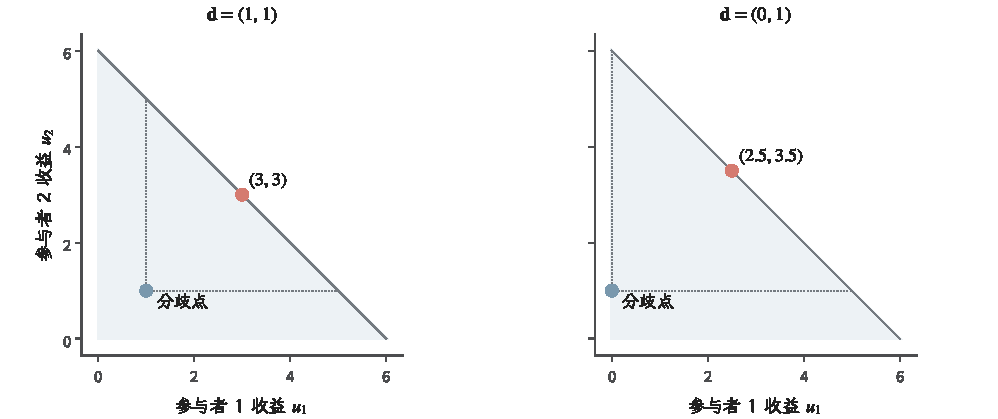
\includegraphics[width=\linewidth]{figures/math-preparation/dynamics/bargaining-disagreement.pdf}
  \caption{两方协商的教学可行域$u_1,u_2\geq0$、$u_1+u_2\leq6$，两图坐标一致。
  蓝点为分歧收益，红点为相对该分歧点的Nash乘积最优解。左图$\bm d=(1,1)$得到
  $(3,3)$，右图$\bm d=(0,1)$得到$(2.5,3.5)$；灰色虚线给出个体可接受的下界。
  可行总收益没有变化，变化的是退出时可得到的收益。}
  \label{fig:game-bargaining-disagreement}
\end{figure*}

没有共同严格正增益时，对数证明不适用，乘积还可能在多个零增益点同时达到最大；若
\(U\)非凸，严格凹性也不能排除不同连通部分上的多个最优点。改变分歧点会改变解，收益
若作一般非线性变换，乘积比较同样会改变。这个“协商解”与非合作博弈中的“Nash均衡”
共享提出者姓名，却解决不同问题。

牌面任务由此可以得到三种互不替代的判断。若参与者对抗，极小极大或Nash均衡检查单方
策略响应；若各方重复学习，遗憾检查相对于某个偏离类的长期损失；若各方合作，Shapley值、
核心或协商解分别按边际贡献、联盟稳定性或分歧点增益分配收益。实际多方系统还可能同时
具有合作与竞争关系，此时必须先写清收益、协调和退出条件，再选择相应解概念。
\section{本章小结}
\label{sec:game-theory-and-multi-agent-decision-summary}
当其他参与者也会选择策略时，行动后果由联合策略决定。有限零和博弈把双方保证值写成
一对线性规划：行方保证收益下界，列方限制收益上界，强对偶使两种证书在同一个博弈值
处相遇。三张牌例子以双方的随机化取得博弈值\(2/3\)，纯策略不能取得这一相互防御。
一般和博弈没有共同博弈值，Nash均衡改为逐人排除单方有利偏离。有限混合策略空间是紧凸
单纯形，Sperner引理与Brouwer定理建立连续不动点，连续近似选择、紧性与闭图再给出
Kakutani路线下的Nash存在性，但不提供唯一性、求解效率或迭代收敛。相关均衡与粗相关
均衡还通过偏离发生在看到建议之前还是之后来区分允许的偏离。
扩展式博弈把行动次序、私人观察和不可区分历史写入信息集。行为策略在每个信息集局部
随机化，Kuhn实现等价说明完全回忆何时使局部表示与完整计划相容。反事实价值去掉自身
到达权重，使少被当前策略访问的信息集仍能比较行动；这种加权不是因果模型中固定外生
背景后的反事实。
重复博弈中的低遗憾是相对于明确比较类的累计保证。投影次梯度由距离平方递推得到
\(O(\sqrt{T})\)外部遗憾；CFR在每个信息集控制即时反事实遗憾。完全回忆使整局偏离
沿本人信息集树分解，由局部正遗憾之和上界全局外部遗憾。两人零和时，加权平均策略趋近
极小极大解；一般和、采样版本和末次迭代需要分别分析。
合作问题改变了待回答的对象。Shapley值在联盟价值已经定义后，平均所有加入次序中的边际
贡献，并由对称性、虚设参与者、有效性和可加性唯一刻画。它不自动保证联盟稳定，
也不把预测归因升级为因果贡献。核心检查联盟是否愿意退出，Pareto条件排除共同改善；
Nash乘积在紧凸且存在共同严格增益时选出唯一收益向量，解仍依赖分歧点。多方决策的结论
须注明收益结构、可用信息、允许偏离和时间口径；只说
“达到均衡”或“分配公平”，不足以确定究竟获得了哪一种保证。
第~\ref{chap:mathematics-and-future-research}章将把前述数学工具按后续研究问题重新组织，
明确不同保证进入学习、推断、迁移与部署时各自控制什么对象。

\chapter{数学基础与后续研究}
\label{chap:mathematics-and-future-research}

前述各章分别研究了函数与极限、空间与变换、随机性与证据、离散结构，以及随时间
演化的状态与行动。把这些内容逐章学会之后，还会留下一个实际问题：面对机器学习中的
某个研究命题，应当从哪一种数学对象开始，又怎样判断一个熟悉的定理能否用于当前设定？

困难不在于记住更多公式，而在于辨认公式所控制的对象。同一个投影既可以描述最小
二乘拟合，也可以描述条件期望；同一个谱既可以揭示数据的低秩方向，也可以刻画动态
系统的衰减模式。公式相似并不表示结论相同。目标函数、观测制度、候选空间和数据
生成过程只要改变一项，原有推导中的条件就可能需要重新核对。

本章按后续研究方向组织这些联系。每节都从一个可手算的小问题出发，指出前文数学进入
推导的位置，并把已经得到的保证与尚待研究章节定义的对象分开。这里不重复前述各章的
完整证明，也不提前展开具体模型的全部训练流程。读者需要形成的是一种工作方式：
先写清研究问题的对象与量词，再找到可复用的数学接口，最后检查接口条件是否真的由
任务、数据和算法满足。

\section{学习理论与泛化}
\label{sec:future-learning-theory-generalization}

\subsection{从候选选择到总体风险}
\label{sec:future-selection-population-risk}

学习理论要回答的不是“训练误差能否算出”，而是“用训练数据选出的函数在新样本上
会怎样”。选择动作使问题发生了变化：对一个事先固定的函数成立的概率界，
未必能直接用于看过同一批数据后才选出的函数。第~\ref{chap:probability-theory}章
建立的同时误差控制，正是从单个随机平均走向数据依赖选择的入口。

设有限候选类为$\mathcal{H}=\{h_1,\ldots,h_M\}$，样本
$Z_1,\ldots,Z_n$独立同分布，损失$\ell(h,Z)\in[0,1]$。记总体风险、经验风险、
经验最优解和类内总体最优解分别为
\begin{align*}
  R(h)&=\mathbb{E}[\ell(h,Z)],\\
  \widehat{R}_n(h)
  &=
  \frac{1}{n}\sum_{i=1}^{n}\ell(h,Z_i),\\
  \widehat{h}
  &\in
  \argmin_{h\in\mathcal{H}}\widehat{R}_n(h),\\
  h^\star
  &\in
  \argmin_{h\in\mathcal{H}}R(h).
\end{align*}
经验最优解依赖全部样本，不能在选择完成后把它当作预先固定的候选。定理
~\ref{thm:probability-finite-class-uniform-bound}已经从Hoeffding不等式和
联合界证明：以至少$1-\delta$的概率，全部$h\in\mathcal H$同时满足
\[
  |R(h)-\widehat R_n(h)|
  \leq
  \varepsilon_n(\delta)
  =
  \sqrt{\frac{\log(2M/\delta)}{2n}}.
\]
在这个同时事件上，把$\widehat h$从总体风险换到经验风险，使用经验最优性与
$h^\star$比较，再换回总体风险，便得到
\begin{equation}
  R(\widehat{h})
  \leq
  R(h^\star)+2\varepsilon_n(\delta).
  \label{eq:future-erm-risk-bound}
\end{equation}
这里不重复第~\ref{chap:probability-theory}章的一般证明；关键接口是误差事件必须
同时覆盖数据选出的$\widehat h$与用于比较的$h^\star$。

实际求解器未必返回精确经验最优解。若$\widetilde h\in\mathcal H$只保证
\[
  \widehat{R}_n(\widetilde h)
  \leq
  \inf_{h\in\mathcal H}\widehat{R}_n(h)+\eta,
\]
则沿同一条比较路径可得
\[
  R(\widetilde h)
  \leq
  R(h^\star)+2\varepsilon_n(\delta)+\eta.
\]
这里的$\eta$来自优化过程，$\varepsilon_n(\delta)$来自有限样本；两项能够进入同一个
上界，不表示它们可由同一种论证减小。

\begin{example}[有限候选中的选择代价]
  \label{ex:future-finite-hypothesis-selection}
  假设$M=8$、$n=200$，并取$\delta=0.05$。代入上式可得
  \[
    \varepsilon_n(\delta)
    =
    \sqrt{\frac{\log 320}{400}}
    \approx 0.120.
  \]
  因而这个简单界只保证
  $R(\widehat h)\leq R(h^\star)+0.240$。若把$M$误写成$1$，
  便会忽略从八个候选中选择所付出的同时控制代价。数值较松不表示推导无效；
  它提示后续研究要利用函数类结构，不能只看候选数。
\end{example}

这个风险差还不是全部学习误差。若真实最优预测规则不在$\mathcal{H}$中，
$R(h^\star)$与所有可测规则中的最优风险之间存在\term{逼近误差}；
有限样本使经验量偏离总体量，产生\term{估计误差}；训练算法若只返回近似经验最优解，
还会产生\term{求解误差}。第~\ref{chap:functional-analysis-and-approximation}章
用函数空间、覆盖和组合复杂度描述前两项之间的结构关系，
第~\ref{chap:optimization}章则分析后一项。三个来源可以相加进入一个上界，
却不能因为都叫“误差”而由同一个定理控制。

\subsection{从有限候选到函数类和算法}
\label{sec:future-function-classes-algorithms}

当$\mathcal{H}$无限时，有限并集界不再直接适用。覆盖数、增长函数和
Rademacher型复杂度通过“在样本分辨率下实际有多少种行为”替代$M$；
算法稳定性改为比较替换一个样本前后的输出；信息论方法则控制算法输出携带了多少
关于训练样本的信息。这些是不同证明路径，不要求同时成立。用有限覆盖代替原函数类时，
覆盖所用的度量还必须能够控制当前损失差；参数空间中的欧氏距离小，本身不保证预测损失
也接近。

\begin{example}[有限选择器的两类控制]
  \label{ex:future-stability-information-finite-selector}
  继续使用例~\ref{ex:future-finite-hypothesis-selection}中的
  \(M=8,n=200\)，先把训练算法\(A\)视为确定性算法，并把输出记为
  \(W=A(S)\in\mathcal H\)。若对任意只相差一个样本的\(S,S'\)和任意测试点\(z\)，
  都有
  \[
    \bigl|
      \ell(A(S),z)-\ell(A(S'),z)
    \bigr|
    \leq\beta,
  \]
  就可用留一替换把稳定性系数接到期望泛化差。具体地，令\(Z_i'\)是\(Z_i\)的
  独立同分布副本，并以\(S^{(i)}\)表示把\(S\)中的\(Z_i\)替换为\(Z_i'\)所得的数据集。
  交换\(Z_i\)与\(Z_i'\)不改变联合分布，因此
  \begin{align*}
    &\left|
      \mathbb{E}\!\left[
        R(A(S))-\widehat R_n(A(S))
      \right]
    \right|
    \\
    &\quad=
    \left|
      \frac1n\sum_{i=1}^n
      \mathbb{E}\!\left[
        \ell(A(S^{(i)}),Z_i)-\ell(A(S),Z_i)
      \right]
    \right|
    \leq\beta.
  \end{align*}
  第~\ref{chap:optimization}章的稳定性路线可以提供这里所需的稳定系数，
  上述替换论证则说明该系数为何控制期望泛化差。
  若\(A\)含内部随机性，可以固定同一个随机种子耦合两次运行并要求上述界对种子成立，
  或改用对算法随机性取期望的稳定性定义；不能省略这一随机性约定。
  这里真正需要核对的是算法对换样本是否敏感。未经正则化的经验风险最小化可能在
  两个经验风险几乎相同的候选之间切换；若它们在某个\(z\)上的损失分别为\(0\)和\(1\)，
  那么一次换样本就可能使上式只能取\(\beta=1\)。候选只有八个并不自动带来小稳定性。

  信息控制考察同一输出\(W\)携带了多少训练样本信息。因为\(W\)至多取八个值，
  \[
    I(W;S)\leq H(W)\leq\log 8.
  \]
  对\([0,1]\)值损失，第~\ref{chap:information-theory-and-statistical-geometry}章的
  换测度界因而给出
  \[
    \left|
      \mathbb{E}\!\left[
        R(W)-\widehat R_n(W)
      \right]
    \right|
    \leq
    \sqrt{\frac{I(W;S)}{2n}}
    \leq
    \sqrt{\frac{\log8}{400}}
    \approx0.072.
  \]
  这个数利用了输出范围有限，却没有证明换一个样本时输出接近。它控制的是期望泛化差，
  也不同于例~\ref{ex:future-finite-hypothesis-selection}中以高概率成立的超额风险界。
  稳定性与互信息可以分析同一个选择器，但条件和结论不能互换。
\end{example}

\subsection{从误差上界到学习与计算的边界}
\label{sec:future-learning-computation-boundaries}

信息论下界进一步说明任何方法需要多少观测\scite{math-cover2006information}，而
第~\ref{chap:combinatorics}章中的计算复杂度讨论给定输入后能否在可接受资源内求出
结果。样本不足与计算困难是两种限制：前者即使给算法无限计算时间也可能无法消除，
后者则可能发生在统计信息已经足够时。

式~\eqref{eq:future-erm-risk-bound}的边界很明确：损失有界、样本独立同分布、
候选类在看见样本前固定，而且使用同一分布定义经验风险和总体风险。
数据依赖地构造候选类、反复查看验证结果、面对相关序列或发生分布迁移时，
都要改用相应的条件化、序贯控制或换测度工具。后续机器学习理论章节将在二分类、
多分类、深层函数类和迁移设定中分别定义可学习对象；本节的推导只提供辨认
“表示、样本、算法与计算”四类问题的起点。

\section{经典模型、核方法与几何表示}
\label{sec:future-classical-kernel-geometric-representation}

\subsection{从拟合目标到投影、谱与正则化}
\label{sec:future-fitting-projection-regularization}

经典模型经常共享平方损失、距离或谱分解，但共享运算不表示共享研究目标。
回归关心预测量与响应之间的误差，降维关心表示保留了什么结构，聚类则需要规定
何种群组关系才算成功。先看一个近共线回归例子，可以同时辨认拟合、敏感性与
正则化分别由哪一部分数学控制。

令设计矩阵与响应为
\[
  \bm{X}
  =
  \begin{bmatrix}
    1 & 1\\
    1 & 1+\varepsilon
  \end{bmatrix},
  \qquad
  \bm{y}
  =
  \begin{bmatrix}
    1\\
    1
  \end{bmatrix},
\]
其中$\varepsilon$很小。两列特征几乎相同，
因此某些系数组合对预测的作用也几乎相同。无正则最小二乘解满足正规方程
\[
  \bm{X}^{\top}\bm{X}\widehat{\bm{w}}
  =
  \bm{X}^{\top}\bm{y}.
\]
矩阵$\bm{X}^{\top}\bm{X}$的行列式为$\varepsilon^2$，
当$\varepsilon\to0$时趋近奇异。第~\ref{chap:linear-algebra}章的投影说明
$\bm{X}\widehat{\bm{w}}$是$\bm{y}$在列空间上的投影，
第~\ref{chap:matrix-analysis}章的奇异值与条件数则说明系数为何对微小扰动敏感。

加入岭正则项后，目标变为
\[
  \min_{\bm{w}\in\mathbb{R}^{2}}
  \frac{1}{2}\lVert\bm{X}\bm{w}-\bm{y}\rVert_2^2
  +
  \frac{\lambda}{2}\lVert\bm{w}\rVert_2^2,
  \qquad \lambda>0,
\]
其唯一解为
\begin{equation}
  \widehat{\bm{w}}_\lambda
  =
  \left(
    \bm{X}^{\top}\bm{X}+\lambda\bm{I}
  \right)^{-1}
  \bm{X}^{\top}\bm{y}.
  \label{eq:future-ridge-solution}
\end{equation}
若$\sigma_j$是$\bm{X}$的奇异值，那么相应谱方向上的逆因子从
$1/\sigma_j^2$变为$1/(\sigma_j^2+\lambda)$。
正则化抑制了小奇异值方向的放大，但也改变了拟合目标。
它改善的是代数条件与系数稳定性，不自动证明新样本上的总体风险更小。

\begin{example}[共线特征的可辨方向]
  \label{ex:future-collinear-ridge}
  取$\varepsilon=0$时，两列完全相同，所有满足$w_1+w_2=1$的向量都给出
  $\bm{X}\bm{w}=\bm{y}$，所以预测值唯一而系数不唯一。加入$\lambda>0$后，
  严格凸性保证岭目标有唯一解，对称性使该解满足$w_1=w_2$，于是
  \[
    \widehat w_{\lambda,1}
    =
    \widehat w_{\lambda,2}
    =
    \frac{2}{4+\lambda}.
  \]
  此时
  \[
    \bm X\widehat{\bm w}_{\lambda}
    =
    \frac{4}{4+\lambda}\bm y,
  \]
  所以有限$\lambda$下的岭解不是零残差解，而是以收缩偏差换取较稳定的系数。
  零残差解集合中的最小范数解是$(1/2,1/2)^{\top}$；只有当
  $\lambda\downarrow0$时，岭解才趋于这个代表。这个结论仍不能说明两个特征具有
  相同的现实含义。
\end{example}

\subsection{从有限特征到核空间中的计算}
\label{sec:future-finite-features-kernel-space}

同一个拟合思想可以从有限维系数扩展到函数空间。设$\mathcal{H}_K$是核$K$对应的
再生核Hilbert空间，考虑
\[
  \min_{f\in\mathcal{H}_K}
  \sum_{i=1}^{n}
  \bigl(f(\bm{x}_i)-y_i\bigr)^2
  +
  \lambda\lVert f\rVert_{\mathcal{H}_K}^{2}.
\]
把任意$f$正交分解为
\[
  f=f_{\parallel}+f_{\perp},
  \qquad
  f_{\parallel}
  \in
  \operatorname{span}
  \{K(\bm{x}_1,\cdot),\ldots,K(\bm{x}_n,\cdot)\}.
\]
再生性质给出
\[
  f_{\perp}(\bm{x}_i)
  =
  \langle
    f_{\perp},K(\bm{x}_i,\cdot)
  \rangle_{\mathcal{H}_K}
  =0.
\]
因此$f$与$f_{\parallel}$在训练点上的损失相同，而
\[
  \lVert f\rVert_{\mathcal{H}_K}^{2}
  =
  \lVert f_{\parallel}\rVert_{\mathcal{H}_K}^{2}
  +
  \lVert f_{\perp}\rVert_{\mathcal{H}_K}^{2}
  \geq
  \lVert f_{\parallel}\rVert_{\mathcal{H}_K}^{2}.
\]
任何最优解都可取成
\begin{equation}
  f^\star(\cdot)
  =
  \sum_{i=1}^{n}\alpha_i K(\bm{x}_i,\cdot).
  \label{eq:future-kernel-representation}
\end{equation}
这段投影推导解释了为什么无限维候选仍能化为$n$个系数，
而不是声称无限维问题本身已经消失。核矩阵的条件数、正则项和求解器仍决定
数值计算是否可靠。

改变核会改变哪些函数被视为平滑或相近，改变正则项则改变同一函数空间中的偏好。
这两种改变分别作用于表示和选择准则。第~\ref{chap:differential-geometry-and-symmetry}章
把距离推广到局部度量、流形与对称结构，
第~\ref{chap:graph-theory}章把邻域关系写成图并用图谱分析变化模式。
它们可用于组织降维或聚类，却不能仅凭“距离保留”推出类别、语义或因果关系也被保留。

\subsection{从预测输出到群组与低维关系}
\label{sec:future-prediction-clusters-low-dimensional-relations}

同一数据矩阵也可以作为无监督分析的对象，但这时目标已经改变。为使误差可以逐项复核，
在上例取\(\varepsilon=1\)，于是
\[
  \bm{X}=
  \begin{bmatrix}
    1&1\\
    1&2
  \end{bmatrix},
  \qquad
  \bm{X}^{\top}\bm{X}=
  \begin{bmatrix}
    2&3\\
    3&5
  \end{bmatrix}.
\]
\(\bm{X}^{\top}\bm{X}\)的两个特征值为
\[
  \sigma_1^2=\frac{7+3\sqrt5}{2},
  \qquad
  \sigma_2^2=\frac{7-3\sqrt5}{2}.
\]
若截断SVD只保留第一项
\(\bm{X}_1=\sigma_1\bm{u}_1\bm{v}_1^{\top}\)，
定理~\ref{thm:matrix-analysis-best-low-rank}给出
\begin{equation}
  \lVert\bm{X}-\bm{X}_1\rVert_{\mathrm F}^2
  =
  \sigma_2^2
  =
  \frac{7-3\sqrt5}{2}
  \approx0.146.
  \label{eq:future-truncated-svd-reconstruction-error}
\end{equation}
这个数是数据矩阵的秩一重构误差，不是回归误差。回归仍使用同一
未中心化矩阵\(\bm{X}\)和\(\bm{y}=(1,1)^{\top}\)，并最小化
\(\lVert\bm{X}\bm{w}-\bm{y}\rVert_2^2\)；此时
\(\bm{w}=(1,0)^{\top}\)使误差为零。若把两行
\((1,1)\)与\((1,2)\)视为样本做不预先中心化的一维降维，式
\eqref{eq:future-truncated-svd-reconstruction-error}衡量的是到所选秩一线性表示的
平方重构误差。若改做单簇聚类，目标又变为到质心
\(\bm m=(1,3/2)^{\top}\)的簇内平方和，其值为
\[
  \lVert(1,1)^{\top}-\bm m\rVert_2^2
  +
  \lVert(1,2)^{\top}-\bm m\rVert_2^2
  =
  \frac12.
\]
输入数据没有改变，但监督响应、低秩表示与离散分组三种输出接口不同，因而三个数不能
互相充当成功标准。

本节例子的结论止于给定样本、给定核与给定正则参数下的表示和求解。
噪声模型、预测区间、超参数选择及总体风险需要统计假设；
聚类和降维还须另行定义群组或结构保真的评价目标。
后续经典模型部分会补上输出语义、数据机制与评价协议。
投影、谱和核是可复用工具，不是这些任务共同的成功标准。

\section{神经网络的结构与表示}
\label{sec:future-neural-structure-representation}

\subsection{从共享局部运算到卷积与等变性}
\label{sec:future-local-operations-convolution-equivariance}

神经网络的结构研究关心怎样把输入中的先验关系写进函数族。
空间平移、节点重编号和时间推进都可表现为“变换输入后，输出应按可预测方式变化”，
但三者作用的对象不同。一个短序列上的共享局部算子可以把张量运算、卷积、
群作用和边界条件连接起来。

考虑长度为$4$的循环序列
\[
  \bm{x}
  =
  \begin{bmatrix}
    x_0 & x_1 & x_2 & x_3
  \end{bmatrix}^{\top}
\]
以及长度为$2$的核$\bm{k}=[k_0,k_1]^{\top}$。
定义循环卷积算子
\[
  (T_{\bm{k}}\bm{x})_i
  =
  k_0x_i+k_1x_{(i-1)\bmod 4}.
\]
令$S$为循环右移一格的置换矩阵，即
$(S\bm{x})_i=x_{(i-1)\bmod4}$。直接代入可得
\begin{align}
  (T_{\bm{k}}S\bm{x})_i
  &=
  k_0x_{(i-1)\bmod4}
  +
  k_1x_{(i-2)\bmod4}
  \nonumber\\
  &=
  (ST_{\bm{k}}\bm{x})_i.
  \label{eq:future-convolution-equivariance}
\end{align}
所以$T_{\bm{k}}S=ST_{\bm{k}}$。
输入平移后，输出发生同样平移，这就是该算子对循环平移的\term{等变性}：
它不要求输出保持不变，而要求输出按规定的群作用同步变化。

\begin{example}[边界条件改变结构关系]
  \label{ex:future-convolution-boundary}
  取$\bm{x}=[1,2,0,0]^{\top}$、$\bm{k}=[1,-1]^{\top}$，
  则
  \[
    T_{\bm{k}}\bm{x}
    =
    [1,1,-2,0]^{\top}.
  \]
  循环右移输入得到$[0,1,2,0]^{\top}$，
  再卷积得到$[0,1,1,-2]^{\top}$，恰好是原输出的循环右移。
  若把循环边界改成左端补零，首尾不再属于同一平移轨道，
  上述交换关系在边界处失效。共享参数本身不足以保证任意边界处理下的精确等变。
\end{example}

第~\ref{chap:signal-analysis}章还说明，循环卷积在离散傅里叶坐标中化为逐频率乘法。
这同时给出表示和计算两种认识：每个频率模式被核的频率响应独立缩放，
而快速变换可以减少某些卷积的运算量。采样或池化随后会改变可分辨频率；
没有抗混叠条件时，低采样率中的低频模式可能来自原信号的多个高频成分。
结构约束限制了函数族，快速算法组织了计算，采样条件决定信息保留，
三者不能合并成一句“卷积保留结构”。

\subsection{从规则序列到图和状态表示}
\label{sec:future-sequences-graphs-state-representations}

输入若由无规则关系构成，变换不再是循环平移，而是节点重编号。
图上的映射$\Phi$若满足
\[
  \Phi(\bm{P}\bm{X},\bm{P}\bm{A}\bm{P}^{\top})
  =
  \bm{P}\Phi(\bm{X},\bm{A})
\]
对允许的置换矩阵$\bm{P}$成立，才具有相应的置换等变性。
第~\ref{chap:graph-theory}章提供邻接、路径、分离与图谱对象，
第~\ref{chap:differential-geometry-and-symmetry}章提供群作用下不变与等变的统一语言。
这条等式只说明重编号一致性，不说明映射能够区分所有不同图结构。

持续到达的序列又引入状态。若
\[
  \bm{s}_{t+1}
  =
  \bm{A}\bm{s}_t+\bm{B}\bm{x}_t,
\]
展开后可得
\[
  \bm{s}_{t}
  =
  \bm{A}^{t}\bm{s}_0
  +
  \sum_{j=0}^{t-1}
  \bm{A}^{t-1-j}\bm{B}\bm{x}_j.
\]
第~\ref{chap:dynamical-systems-and-state-estimation}章的谱与Lyapunov工具
判断历史扰动如何衰减或放大。这个状态核与卷积形式相似，
但当$\bm{A}$随输入或时间改变时，固定卷积核不再描述完整递推。

\subsection{从复合映射到敏感性与逼近能力}
\label{sec:future-composition-sensitivity-approximation}

结构确定后，还要判断复合映射对输入扰动的局部响应。
对
\[
  \bm{h}=f(\bm{x}),
  \qquad
  \bm{y}=g(\bm{h}),
\]
链式法则给出
\[
  \bm{J}_{g\circ f}(\bm{x})
  =
  \bm{J}_{g}(\bm{h})\bm{J}_{f}(\bm{x}),
\]
进而有局部范数界
\[
  \lVert\bm{J}_{g\circ f}(\bm{x})\rVert_2
  \leq
  \lVert\bm{J}_{g}(\bm{h})\rVert_2
  \lVert\bm{J}_{f}(\bm{x})\rVert_2.
\]
它控制局部敏感性，却不等价于第~\ref{chap:functional-analysis-and-approximation}章
讨论的逼近能力。一个函数族可能足以逼近目标，但具体参数对应的映射仍很敏感；
也可能满足严格等变性，却因结构约束过强而无法表达任务所需关系。

本节只说明算子结构可检查的代数关系。后续神经网络模型部分仍须定义具体层、
状态、注意机制或消息传递过程，并说明计算代价与任务证据。
等变性不推出不变性，局部Jacobian矩阵界不推出全局鲁棒性，
状态稳定也不推出表示包含了预测所需的全部信息。

\section{神经网络的训练与泛化}
\label{sec:future-neural-training-generalization}

\subsection{从反向求导到下降与曲率}
\label{sec:future-backpropagation-descent-curvature}

结构规定了候选函数怎样计算，训练则要从数据中选出参数。
这一步至少包含四个不同问题：导数是否算对，单步更新是否下降，
带噪迭代是否长期稳定，以及最终函数是否能泛化。
它们共享同一参数，却由不同数学条件支撑。

考虑一个标量输入、单隐藏单元的两层映射
\[
  f_{w,v}(x)=v\sigma(wx),
\]
以及单样本平方损失
\[
  L(w,v)
  =
  \frac{1}{2}\bigl(f_{w,v}(x)-y\bigr)^2.
\]
记误差$e=v\sigma(wx)-y$。在$\sigma$可微处，
链式法则给出
\begin{equation}
  \frac{\partial L}{\partial v}
  =
  e\sigma(wx),
  \qquad
  \frac{\partial L}{\partial w}
  =
  ev\sigma'(wx)x.
  \label{eq:future-two-layer-gradient}
\end{equation}
这只是导数计算。若$\sigma$在某点不可微，需要选用次梯度、
平滑替代或明确的人为替代梯度；三种做法改变的数学对象并不相同。

这个具体网络是否满足下降引理的光滑条件，可以直接由二阶导数核对。仍令
\(\bm\theta=(w,v)^{\top}\)，并把\(\sigma,\sigma',\sigma''\)都理解为在\(wx\)处取值。
在\(\sigma\)二阶可微处，
\[
  \nabla^2 L(w,v)
  =
  \begin{bmatrix}
    v^2x^2(\sigma')^2+evx^2\sigma''
    &
    x\sigma'(2v\sigma-y)
    \\
    x\sigma'(2v\sigma-y)
    &
    \sigma^2
  \end{bmatrix}.
\]
固定\(x,y\)，若某个包含当前参数的凸紧邻域\(U\)使\(wx\)始终落在
\(\sigma\)的二阶连续可微区间内，那么\(w,v,\sigma,\sigma'\)和\(\sigma''\)
在\(U\)上都有界，以上Hessian矩阵的算子范数也有有限上界\(L_U\)。
第~\ref{chap:mathematical-analysis}章的中值估计于是给出
\[
  \lVert\nabla L(\bm\theta)-\nabla L(\bm\theta')\rVert_2
  \leq
  L_U\lVert\bm\theta-\bm\theta'\rVert_2,
  \qquad
  \bm\theta,\bm\theta'\in U.
\]
所以这个两层网络在该邻域内满足梯度Lipschitz条件，但要使用局部常数\(L_U\)，
还须保证更新没有离开\(U\)。即使\(\sigma,\sigma',\sigma''\)全局有界，
上式中的\(v^2\)也说明不限制\(v\)时不能由此得到全局光滑常数；若使用ReLU且
\(x\neq0\)，跨过\(wx=0\)的邻域中一般不存在上述经典Hessian矩阵。

设把参数合并为$\bm\theta=(w,v)^{\top}$，
目标$F(\bm\theta)$的梯度是$L_F$-Lipschitz的。
梯度更新
\[
  \bm{\theta}^{(t+1)}
  =
  \bm{\theta}^{(t)}
  -
  \eta\nabla F(\bm{\theta}^{(t)})
\]
结合光滑性上界可得
\begin{align}
  F(\bm{\theta}^{(t+1)})
  &\leq
  F(\bm{\theta}^{(t)})
  -
  \eta\lVert\nabla F(\bm{\theta}^{(t)})\rVert_2^2
  +
  \frac{L_F\eta^2}{2}
  \lVert\nabla F(\bm{\theta}^{(t)})\rVert_2^2
  \nonumber\\
  &=
  F(\bm{\theta}^{(t)})
  -
  \eta
  \left(1-\frac{L_F\eta}{2}\right)
  \lVert\nabla F(\bm{\theta}^{(t)})\rVert_2^2.
  \label{eq:future-gradient-descent-one-step}
\end{align}
当$0<\eta<2/L_F$时，右端不增。
第~\ref{chap:optimization}章给出了这种下降论证及凸性、PL条件等进一步接口；
非凸目标仅有单步下降，通常不足以推出到达全局最优解。

\begin{example}[步长跨过下降范围]
  \label{ex:future-training-step-size}
  对$F(\theta)=\theta^2/2$，梯度为$\theta$且$L_F=1$。
  更新后$\theta^{(t+1)}=(1-\eta)\theta^{(t)}$，
  因而
  \[
    \frac{F(\theta^{(t+1)})}{F(\theta^{(t)})}
    =
    (1-\eta)^2.
  \]
  取$\eta=1$时一步到达零点，取$\eta=3$时目标放大为原来的四倍。
  梯度方向没有算错，失败来自步长不满足下降条件。
\end{example}

曲率矩阵的谱决定不同方向上的尺度差异。若局部二次模型中的Hessian矩阵
\(\bm H=\bm H^{\top}\succ\bm0\)，且近似为
\[
  F(\bm{\theta}+\bm{\Delta})
  \approx
  F(\bm{\theta})
  +
  \langle\nabla F(\bm{\theta}),\bm{\Delta}\rangle
  +
  \frac{1}{2}
  \bm{\Delta}^{\top}\bm{H}\bm{\Delta},
\]
那么\(\bm H\)的最大与最小特征值之比较刻画各方向的曲率尺度；条件数较大时，
统一步长受最大曲率方向限制，而在小曲率方向上推进较慢。取对称正定矩阵
\(\bm P\in\mathbb{R}^{2\times2}\)，预条件更新
\[
  \bm{\theta}^{(t+1)}
  =
  \bm{\theta}^{(t)}
  -
  \eta\bm{P}^{-1}\nabla F(\bm{\theta}^{(t)})
\]
试图改变局部坐标中的尺度。第~\ref{chap:matrix-analysis}章说明
$\bm{P}$的谱与数值求解条件；具体下降保证仍须结合预条件后的谱界和步长。
若\(\bm H\)不定，则还存在负曲率方向，不能沿用正定二次模型的条件数解释，
下降与收敛也需要另行分析。

\subsection{从小批量梯度到随机逼近和分布几何}
\label{sec:future-minibatch-stochastic-approximation-geometry}

第~\ref{chap:information-theory-and-statistical-geometry}章把Fisher度量解释为参数
变化引起的局部分布变化。
经验梯度的二阶矩只有在相应概率模型与取期望条件下才与Fisher信息对应，
不能仅因矩阵外形相同便互换。

\begin{example}[同一参数点上的三种二次量]
  \label{ex:future-parameter-second-moment-fisher}
  沿用上一小节的两层映射，取\(\sigma(u)=u\)、\(x=1\)，并把
  \(f_{w,v}(x)=vw\)作为Bernoulli模型的对数几率：
  \[
    p_{\bm\theta}(Y=1\mid x)
    =
    \frac{1}{1+\exp\{-f_{w,v}(x)\}}.
  \]
  在\(\bm\theta_0=(1,\log4)^{\top}\)处，正类概率为\(p=0.8\)，且
  \[
    \bm J
    =
    \nabla_{\bm\theta}f_{\bm\theta_0}(x)
    =
    \begin{bmatrix}\log4\\1\end{bmatrix}.
  \]
  对同一小扰动\(\bm\Delta=(\varepsilon,0)^{\top}\)，欧氏参数距离只记录坐标变化，
  \[
    \lVert\bm\Delta\rVert_2^2=\varepsilon^2.
  \]

  若当前观察到\(Y=1\)，负对数似然梯度为
  \(\bm g_1=(p-1)\bm J=-0.2\bm J\)。这个观测形成的梯度二阶矩为
  \(\bm G_{\mathrm{obs}}=\bm g_1\bm g_1^{\top}\)，故
  \[
    \bm\Delta^{\top}\bm G_{\mathrm{obs}}\bm\Delta
    =
    0.04(\log4)^2\varepsilon^2
    \approx0.0769\varepsilon^2.
  \]
  Fisher信息则对模型自身的随机标签取期望：
  \[
    \bm F(\bm\theta_0)
    =
    \mathbb{E}_{Y\sim p_{\bm\theta_0}}
    [\bm g_Y\bm g_Y^{\top}]
    =
    p(1-p)\bm J\bm J^{\top},
  \]
  因而
  \[
    \bm\Delta^{\top}\bm F(\bm\theta_0)\bm\Delta
    =
    0.16(\log4)^2\varepsilon^2
    \approx0.3075\varepsilon^2.
  \]
  三个量在同一参数点和同一方向上仍不相等：欧氏距离依赖参数坐标，
  观测梯度二阶矩依赖实际样本，Fisher二次型则是模型分布下得分的期望，
  它的一半给出局部KL变化的二阶主项。只有损失确为该模型的负对数似然，并按模型分布
  对观测取期望时，后两种矩阵才对应。
\end{example}

小批量训练把精确梯度改成随机估计
\[
  \bm{g}^{(t)}
  =
  \nabla F(\bm{\theta}^{(t)})
  +
  \bm{\xi}^{(t)}.
\]
若条件均值满足
$\mathbb{E}[\bm{\xi}^{(t)}\mid\mathcal{F}_t]=\bm{0}$，
步长满足相应求和条件，并且迭代有界或存在稳定机制，
第~\ref{chap:stochastic-processes-and-approximation}章的随机逼近工具
可把更新与平均动力学联系起来。批量改变时，噪声方差和相关结构也会改变；
仅验证无偏，不能替代矩条件、步长和稳定性。

\subsection{从训练收敛到新样本表现}
\label{sec:future-training-convergence-generalization}

即使训练目标持续下降，也只说明当前数据上的求解行为。
把训练所得函数用于新样本，需要回到
式~\eqref{eq:probability-finite-class-bound}一类泛化工具，
或采用函数类复杂度、稳定性和信息控制等其他路径。
参数数量、参数范数、谱量和优化轨迹可以成为分析量，
但任何一个量单独变小都不自动推出总体风险变小。

后续神经网络训练章节会指定初始化、归一化、数据变换、损失与停止规则，
深度学习理论则针对具体函数类和随机算法建立结论。
本节的边界是：式~\eqref{eq:future-two-layer-gradient}只保证局部导数正确，
式~\eqref{eq:future-gradient-descent-one-step}只在光滑性和步长条件下保证单步变化，
随机逼近讨论长期迭代，而泛化仍需单独的数据生成假设。

\section{概率模型的推断、学习与生成}
\label{sec:future-probabilistic-inference-learning-generation}

\subsection{从联合模型到条件查询和结构计算}
\label{sec:future-joint-model-conditional-query}

概率模型中的“计算概率”“从数据估计参数”和“生成新样本”常使用同一个联合分布，
却回答三个不同问题。先固定一个含隐变量的简单模型，
可以看清边缘化、条件化、参数学习和采样各自改变了什么。

设隐变量$Z\in\{0,1\}$，观测$X\in\{0,1\}$，
\[
  \mathbb{P}(Z=1)=\pi,
  \qquad
  \mathbb{P}(X=1\mid Z=z)=\theta_z.
\]
参数$\pi,\theta_0,\theta_1$给定时，边缘概率由全概率公式得到
\[
  \mathbb{P}(X=1)
  =
  (1-\pi)\theta_0+\pi\theta_1.
\]
观察到$X=1$后，对隐状态的条件推断为
\begin{equation}
  \mathbb{P}(Z=1\mid X=1)
  =
  \frac{\pi\theta_1}
  {(1-\pi)\theta_0+\pi\theta_1}.
  \label{eq:future-latent-posterior}
\end{equation}
这里没有学习参数，只是对给定联合分布执行求和与条件化。

\begin{example}[同一联合分布上的三个问题]
  \label{ex:future-latent-three-questions}
  取$\pi=1/4$、$\theta_0=1/5$、$\theta_1=4/5$。
  则
  \[
    \mathbb{P}(X=1)
    =
    \frac{3}{4}\frac{1}{5}
    +
    \frac{1}{4}\frac{4}{5}
    =
    \frac{7}{20},
  \]
  且
  \[
    \mathbb{P}(Z=1\mid X=1)
    =
    \frac{(1/4)(4/5)}{7/20}
    =
    \frac{4}{7}.
  \]
  推断问的是已见$X=1$时$Z$如何分布；学习会把三个参数视为未知；
  生成则先抽$Z$，再按对应$\theta_Z$抽$X$。三个过程共用因子，
  输入、输出和正确性标准却不同。
\end{example}

变量增多后，直接枚举联合状态的代价可能迅速增大。
第~\ref{chap:graph-theory}章中的分离、消元与分配结构
把全局求和重组为局部运算。计算量取决于消元过程中形成的中间作用域，
而不只取决于原图有多少条边。连续变量还要核对积分交换与可积性；
线性高斯结构可利用第~\ref{chap:matrix-analysis}章的Schur补，
动态结构则可复用第~\ref{chap:dynamical-systems-and-state-estimation}章的
预测、滤波与平滑递推。

同一联合分解还会因查询目标不同而使用不同运算。计算某个变量的边缘概率时，
需要对其余变量求和；求联合最大后验配置时，要把消元中的求和改为最大化，并保存
每一步的最优见证以便回溯出彼此兼容的联合配置。逐时边缘最优状态则先分别计算各时刻的
边缘分布，再在每个边缘上取最大值；这些状态通常不能直接拼成联合概率最大的整条路径。
求和与最大化一般不可交换，因此图结构只规定可利用的分解，查询目标还决定消元代数、
回溯信息和最终输出。

\subsection{从精确查询到三类近似}
\label{sec:future-exact-query-three-approximations}

精确边缘难以计算时，可以引入近似分布$q(z)$。
假设$0<p(x)<\infty$，并且$q$与后验$p(\cdot\mid x)$具有相同支撑，即
$q(z)>0$当且仅当$p(x,z)>0$；再假设下述期望与KL散度有限，则
\begin{align}
  \log p(x)
  &=
  \log
  \sum_z
  q(z)\frac{p(x,z)}{q(z)}
  \nonumber\\
  &\geq
  \sum_z
  q(z)
  \log\frac{p(x,z)}{q(z)}
  =
  \mathcal{L}(q),
  \label{eq:future-elbo}
\end{align}
其中不等式来自对数函数的凹性。进一步整理可得
\[
  \log p(x)-\mathcal{L}(q)
  =
  \operatorname{KL}\bigl(q(z)\,\|\,p(z\mid x)\bigr).
\]
因此优化变分下界等价于在所选$q$族内逼近后验，
但只有当$q$族包含真实后验且优化到全局最优时，间隙才必为零。
第~\ref{chap:information-theory-and-statistical-geometry}章提供
KL散度与变分表达，第~\ref{chap:optimization}章提供交替和分布优化的求解接口。

另一条路径是用样本平均近似期望。若
$Z^{(1)},\ldots,Z^{(N)}$来自目标分布且二阶矩有限，
\[
  \widehat\mu_N
  =
  \frac{1}{N}
  \sum_{j=1}^{N}f(Z^{(j)})
\]
在独立抽样下具有方差
$\operatorname{Var}(f(Z))/N$。
若样本来自Markov链，相关性会改变有效方差，
需要第~\ref{chap:stochastic-processes-and-approximation}章的遍历与相关平均条件。
链保持目标分布并不说明有限步已经充分混合，
有限样本误差也不能由平稳性一项保证。

连续后验还可以在众数附近作局部二次展开。若
\[
  \widehat{\bm z}
  \in
  \argmax_{\bm z}\log p(\bm z\mid x),
  \qquad
  \bm H
  =
  -\nabla^2_{\bm z}\log p(\widehat{\bm z}\mid x)
\]
且$\widehat{\bm z}$是内点、$\bm H$正定，二阶Taylor展开给出局部高斯近似
\[
  p(\bm z\mid x)
  \approx
  \mathcal N(\widehat{\bm z},\bm H^{-1}).
\]
第~\ref{chap:mathematical-statistics}章的Laplace近似说明，还需有足够光滑性，并且
后验主要质量确由该邻域控制。多峰、边界众数或退化曲率都会破坏这一近似。
变分法限制分布族，采样法以随机平均逼近期望，Laplace方法只保留局部曲率；
三者改变的对象和误差来源不同。

\begin{example}[同一后验上的三种近似]
  \label{ex:future-posterior-approximation-comparison}
  取先验\(p\sim\operatorname{Beta}(2,2)\)，观察四次Bernoulli试验中的三次成功，
  则同一个精确后验为
  \[
    p\mid\bm y\sim\operatorname{Beta}(5,3),
    \qquad
    \mathbb{E}[p\mid\bm y]=\frac58,
    \qquad
    \operatorname{Var}(p\mid\bm y)=\frac{15}{576}.
  \]
  以下记其密度为\(\pi(p\mid\bm y)\)。
  若变分族取全部Beta分布，ELBO的全局最优解就是
  \(q^\star=\operatorname{Beta}(5,3)\)，其分布逼近误差
  \(\operatorname{KL}(q^\star\Vert \pi(\cdot\mid\bm y))\)为零。这个结果依赖候选族
  包含精确后验；换成受限族后，ELBO间隙衡量的是所选方向的KL误差。

  若能独立采样，\(N\)个后验样本的均值估计后验均值，其Monte Carlo标准误为
  \[
    \sqrt{\frac{15}{576N}}.
  \]
  取\(N=100\)时约为\(0.0161\)。这里控制的是某个后验期望的随机积分误差，
  不是一个固定近似密度与精确后验之间的距离。

  Laplace方法在后验众数\(\widehat p=2/3\)处展开。负对数后验的局部曲率为
  \[
    -\left.
    \frac{\mathrm d^2}{\mathrm dp^2}
    \log \pi(p\mid\bm y)
    \right|_{p=2/3}
    =
    \frac{4}{(2/3)^2}+\frac{2}{(1/3)^2}
    =27,
  \]
  因而得到\(\mathcal N(2/3,1/27)\)。其均值相对精确后验偏高
  \(1/24\)，方差相差
  \[
    \frac1{27}-\frac{15}{576}
    =
    \frac{19}{1728}
    \approx0.0110.
  \]
  它还把少量质量放到参数区间\([0,1]\)之外。Laplace误差来自局部二次形状无法完整
  表示偏斜与边界，而非有限样本平均的随机波动。
\end{example}

\subsection{从参数估计到样本构造}
\label{sec:future-parameter-estimation-sample-generation}

参数未知时，问题转为根据观测识别和估计
$\pi,\theta_0,\theta_1$。仅观察$X$时，
不同参数组合可能产生同一个边缘Bernoulli概率，
所以更多样本只能更精确地估计这个边缘量，不能自动区分不可识别的参数。
第~\ref{chap:mathematical-statistics}章把识别、似然、缺失机制和估计误差分开；
交替优化只能求解给定目标，不能修复目标本身的不可识别性。

在这个隐变量模型中，交替精确更新为何单调改善观测似然也可以就地核对。对观测
\(x_1,\ldots,x_n\)，记参数为\(\bm\vartheta=(\pi,\theta_0,\theta_1)\)，并定义
\[
  \ell_{\mathrm{obs}}(\bm\vartheta)
  =
  \sum_{i=1}^{n}
  \log\sum_{z\in\{0,1\}}
  p_{\bm\vartheta}(x_i,z).
\]
设各次迭代中的边缘似然严格为正且有限，后验和下列期望均有定义，并且两个条件
子问题的最优解能够达到。精确E步和M步分别取
\[
  q_i^{(t+1)}(z)
  =
  p_{\bm\vartheta^{(t)}}(z\mid x_i),
  \qquad
  \bm\vartheta^{(t+1)}
  \in
  \argmax_{\bm\vartheta}
  \mathcal L(\bm q^{(t+1)},\bm\vartheta),
\]
其中
\[
  \mathcal L(\bm q,\bm\vartheta)
  =
  \sum_{i=1}^{n}\sum_z
  q_i(z)
  \log
  \frac{p_{\bm\vartheta}(x_i,z)}{q_i(z)}.
\]
变分恒等式给出
\[
  \ell_{\mathrm{obs}}(\bm\vartheta)
  =
  \mathcal L(\bm q,\bm\vartheta)
  +
  \sum_{i=1}^{n}
  \operatorname{KL}\!\left(
    q_i\,\middle\|\,
    p_{\bm\vartheta}(\,\cdot\mid x_i)
  \right).
\]
E步使右端的KL项在\(\bm\vartheta^{(t)}\)处为零，M步又精确提高同一个下界，因而
\begin{align*}
  \ell_{\mathrm{obs}}(\bm\vartheta^{(t)})
  &=
  \mathcal L(\bm q^{(t+1)},\bm\vartheta^{(t)})
  \\
  &\leq
  \mathcal L(\bm q^{(t+1)},\bm\vartheta^{(t+1)})
  \\
  &\leq
  \ell_{\mathrm{obs}}(\bm\vartheta^{(t+1)}).
\end{align*}
这就是单调改善的完整理由；一般交替与主化--最小化论证见
第~\ref{chap:optimization}章。等号可以连续成立，所以该链条不保证严格改善，
也不保证到达全局最大值。若E步不是当前参数的精确后验，或M步没有提高同一个
\(\mathcal L\)，上述两处依据都要重新检查。

生成样本又改变了输出要求。可逆变换依赖Jacobian矩阵与密度换元，
连续随机生成依赖布朗运动、随机微分与密度演化，
而直接祖先采样依赖图中的条件分解。一个过程具有正确的不变分布、
一个变分目标足够高，或一个数值积分器局部误差较小，
都不能单独替代对生成分布与任务质量的评价。
后续概率图模型部分将定义具体表示与算法；本节只建立区分
建模误差、推断误差、参数误差、采样误差和数值误差的框架。

\section{可信机器学习}
\label{sec:future-trustworthy-machine-learning}

\subsection{从预测误差到覆盖与验证证据}
\label{sec:future-prediction-error-coverage-evidence}

平均预测误差只回答随机抽取一个样本时的平均表现。
可信机器学习会进一步询问：预测范围是否覆盖未来结果，输入受扰动后输出是否稳定，
不同群组或干预目标是否得到规定保障，算法输出是否泄露单个数据主体的信息。
这些要求没有共同的单一分数，必须先固定保护或保证的对象。

先看有限样本预测覆盖。设有$n$个校准分数
$S_1,\ldots,S_n$和一个未来分数$S_{n+1}$，
且$n+1$个分数可交换。若分数越大表示预测越不相容，
令
\[
  k=\left\lceil(n+1)(1-\alpha)\right\rceil,
\]
当$k\leq n$时取排序阈值$q=S_{(k)}$，并令预测集合包含所有分数不超过$q$的候选结果；
当$k=n+1$时约定$q=+\infty$，即返回整个候选结果空间。后一约定处理
$\alpha<1/(n+1)$的极端置信水平，此时有限校准样本无法给出非平凡的分布无关集合。
由于未来分数的秩在无并列的情形下均匀分布于
$\{1,\ldots,n+1\}$，
\begin{equation}
  \mathbb{P}(S_{n+1}\leq q)
  =
  \begin{cases}
    k/(n+1), & k\leq n,\\
    1, & k=n+1,
  \end{cases}
  \geq
  1-\alpha.
  \label{eq:future-exchangeable-coverage}
\end{equation}
有并列时采用适当随机化或保守规则，仍可得到相应覆盖结论。

\begin{example}[四个可交换分数的秩]
  \label{ex:future-conformal-rank}
  设$n=3$、$\alpha=1/4$，三个校准分数排序后为
  $0.2,0.5,0.9$。此时$k=\lceil4\times3/4\rceil=3$，
  阈值为$0.9$。若四个分数可交换且没有并列，
  未来分数落在前三级秩中的概率为$3/4$。
  这个计算给出边缘覆盖；它没有声称对每个固定输入、每个群组或每个时间点
  都具有$3/4$的条件覆盖。
\end{example}

式~\eqref{eq:future-exchangeable-coverage}依赖可交换性与预先规定的构造。
若校准样本与未来样本来自不同分布，或者反复查看校准表现后选择分数函数，
秩的对称性会被破坏。第~\ref{chap:probability-theory}章提供可交换秩，
第~\ref{chap:mathematical-statistics}章则说明数据划分、模型选择、
多重比较与持续查看怎样影响证据。总体覆盖不能仅通过按群组报告平均值
升级为条件覆盖。

\subsection{从允许扰动到群组与行为要求}
\label{sec:future-perturbations-groups-behavior}

鲁棒性把问题改成允许输入在集合内变化时，输出最多改变多少。
若可微标量函数$f$在$\bm{x}$附近作一阶展开，
\[
  f(\bm{x}+\bm{\delta})-f(\bm{x})
  \approx
  \langle\nabla f(\bm{x}),\bm{\delta}\rangle.
\]
对约束$\lVert\bm{\delta}\rVert_p\leq\varepsilon$，
对偶范数关系给出
\begin{equation}
  \sup_{\lVert\bm{\delta}\rVert_p\leq\varepsilon}
  \langle\nabla f(\bm{x}),\bm{\delta}\rangle
  =
  \varepsilon
  \lVert\nabla f(\bm{x})\rVert_q,
  \qquad
  \frac{1}{p}+\frac{1}{q}=1.
  \label{eq:future-dual-norm-robustness}
\end{equation}
第~\ref{chap:linear-algebra}章给出范数与对偶范数，
第~\ref{chap:optimization}章把扰动集合接入约束或鞍点目标。
式~\eqref{eq:future-dual-norm-robustness}是线性项的精确最坏变化；
对有限扰动下的非线性模型，还要控制Taylor余项或给出有效的全局Lipschitz界。

公平性可能要求比较群组条件错误率，也可能要求某种干预或反事实量。
前者依赖条件概率及分母，后者还依赖第~\ref{chap:causal-inference}章的识别假设。
仅让两个观测群组的某项平均相等，不能推出个体在干预意义下受到相同处理。
行动补救也不只是寻找梯度方向：候选改变必须可实施，
并且改变后预测的因果含义需要由结构假设支持。

对齐、拒答和安全决策把概率输出继续接到损失、行动与风险。
第~\ref{chap:decision-theory-and-dynamic-risk}章说明同一预测分布可以对应
不同错误代价和风险准则，第~\ref{chap:control-theory}章则区分长期稳定、
成本最优与安全集合保持。

\subsection{从数据变化到隐私与解释对象}
\label{sec:future-data-changes-privacy-explanation}

隐私保护则比较相邻数据集$D,D'$下随机算法的输出分布。给定一个对称的相邻关系，
若\(\epsilon\geq0\)、\(\delta\in[0,1]\)，且随机机制\(\mathcal M\)对任意相邻的
\(D,D'\)和任意可测输出事件\(A\)都满足
\[
  \mathbb{P}(\mathcal{M}(D)\in A)
  \leq
  e^\epsilon
  \mathbb{P}(\mathcal{M}(D')\in A)+\delta,
\]
就称\(\mathcal M\)满足\((\epsilon,\delta)\)-差分隐私
（differential privacy, DP）。其中\(e^\epsilon\)限制输出概率的乘性变化，
\(\delta\)允许一个加性例外；两者越小，相邻数据集的输出分布越难区分。
应用这一定义前，研究者必须先说明何种数据变化构成相邻。
改变保护单位会改变敏感度与噪声尺度；
分布差异和信息控制可以组织证明，但不能替代威胁模型。
类似地，可解释性中的局部导数、估计影响和联盟贡献分别解释
输入敏感性、训练过程与预先定义的价值函数，不能共用一个含混的“重要性”概念。

\begin{example}[同一预测上的三种解释对象]
  \label{ex:future-explanation-three-objects}
  考虑带交互项的预测
  \[
    f_{\bm w}(\bm x)
    =
    w_1x_1+w_2x_2+w_{12}x_1x_2,
    \qquad
    \bm w=(1,2,1)^{\top},
  \]
  并解释目标输入\(\bm x=(1,1)^{\top}\)处的预测\(f_{\bm w}(\bm x)=4\)。
  局部导数把训练结果\(\bm w\)固定，只改变输入的第一个特征：
  \[
    \frac{\partial f_{\bm w}}{\partial x_1}(1,1)
    =
    w_1+w_{12}x_2
    =
    2.
  \]
  它表示\(x_1\)在该点每作一个无穷小单位变化时，预测的一阶变化率。

  影响函数改变的是训练分布。为使数值可复核，设单点损失为半平方损失
  \[
    \ell(\bm w;(\bm x,y))
    =
    \frac12\bigl(f_{\bm w}(\bm x)-y\bigr)^2,
  \]
  \(\bm w\)由相应总体风险估计，且该总体风险的参数Hessian矩阵在当前解处为
  \(\bm I_3\)。若给训练点
  \(z=((1,0)^{\top},4)\)增加无穷小概率质量，则该点的参数梯度为
  \[
    \nabla_{\bm w}\ell(\bm w;z)
    =
    \bigl(f_{\bm w}(1,0)-4\bigr)
    \begin{bmatrix}1\\0\\0\end{bmatrix}
    =
    \begin{bmatrix}-3\\0\\0\end{bmatrix}.
  \]
  第~\ref{chap:mathematical-statistics}章的影响函数公式给出参数的一阶变化
  \(3(1,0,0)^{\top}\)，进而使目标输入处的预测以速率\(3\)变化。
  这里被扰动的是训练点权重，而不是目标输入的\(x_1\)。

  Shapley解释还要先指定缺失特征的基线。取零基线并令
  \(v(S)=f_{\bm w}(\bm x_S,\bm0_{\bar S})-f_{\bm w}(\bm0)\)，则
  \[
    v(\varnothing)=0,\quad
    v(\{1\})=1,\quad
    v(\{2\})=2,\quad
    v(\{1,2\})=4.
  \]
  第~\ref{chap:game-theory-and-multi-agent-decision}章的两人Shapley公式因此给出
  \[
    \phi_1
    =
    \frac12[(1-0)+(4-2)]
    =
    \frac32,
    \qquad
    \phi_2=\frac52.
  \]
  它把相对基线的有限预测差\(4\)分配给两个特征，并把交互项在两种加入次序间平均。
  数值\(2,3,3/2\)不同并非矛盾：三者分别回答局部输入扰动、训练分布污染和
  基于指定联盟价值的有限贡献。
\end{example}

后续可信性章节仍须逐项规定保护对象、威胁条件、
数据协议和验证程序。本节给出的覆盖与扰动推导不能被拼成一个无定义的总体可信保证。

\section{强化学习与序贯决策}
\label{sec:future-reinforcement-learning-sequential-decision}

\subsection{从两步决策到固定点与占用流量}
\label{sec:future-two-step-fixed-point-occupancy}

监督预测把数据分布视为给定，序贯决策中的行动却会改变后续状态和未来数据。
因此，价值递推、随机逼近、探索证据、离线支持和安全约束必须在同一个时间结构中
分别核对\scite{sutton2018}先从一个已知模型的两阶段过程出发，可以确定动态规划
究竟解决了哪一步。

设初始状态为$s$，可选行动$a$，
即时奖励为$r(s,a)$，下一状态按
$P(s'\mid s,a)$分布。最后阶段的价值为
\[
  V_1(s)
  =
  \max_a r_1(s,a).
\]
初始阶段的最优价值则为
\begin{equation}
  V_0(s)
  =
  \max_a
  \left\{
    r_0(s,a)
    +
    \sum_{s'}P(s'\mid s,a)V_1(s')
  \right\}.
  \label{eq:future-two-stage-bellman}
\end{equation}
这一步来自条件期望和“在下一状态到达后再选择”的信息顺序。
若初始行动必须在看见$s'$之前同时承诺第二步行动，
最大值与期望的次序就会改变。

\begin{example}[即时奖励与未来价值]
  \label{ex:future-two-stage-decision}
  初始状态有行动$a$和$b$。行动$a$立即得到$1$，
  随后以相同概率到达终局价值$0$或$4$的状态；
  行动$b$立即得到$2$，随后确定到达终局价值$1$的状态。
  由式~\eqref{eq:future-two-stage-bellman}，
  \[
    Q_0(s,a)=1+\frac{0+4}{2}=3,
    \qquad
    Q_0(s,b)=2+1=3.
  \]
  两个行动的期望价值相同，但尾部风险不同。
  若改用动态风险准则，还要明确条件风险怎样逐阶段嵌套，
  不能只把期望符号替换为一个静态风险数。
\end{example}

在折扣无限时域中，对有界函数$V$定义Bellman最优算子
\[
  (\mathcal{T}V)(s)
  =
  \max_a
  \left\{
    r(s,a)
    +
    \gamma
    \sum_{s'}P(s'\mid s,a)V(s')
  \right\},
  \qquad 0\leq\gamma<1.
\]
利用最大值的差不超过对应项最大差，可得
\[
  \lVert\mathcal{T}V-\mathcal{T}W\rVert_\infty
  \leq
  \gamma\lVert V-W\rVert_\infty.
\]
第~\ref{chap:mathematical-analysis}章的压缩映射定理于是给出固定点唯一性
与值迭代误差收缩。这个结论以已知转移核、奖励有界和$\gamma<1$为前提；
平均回报、无折扣或连续状态问题需要不同的空间与条件。

同一个有限状态、有限动作的折扣问题还可从流量角度表达。给定归一化初始分布
$\rho$，以$(1-\gamma)\sum_s\rho(s)V(s)$为最小化目标，并加入价值不等式
\[
  V(s)
  \geq
  r(s,a)
  +
  \gamma\sum_{s'}P(s'\mid s,a)V(s')
\]
组成一个线性规划；其对偶变量$d(s,a)\geq0$满足
\begin{equation}
  \sum_a d(s,a)
  =
  (1-\gamma)\rho(s)
  +
  \gamma
  \sum_{\bar s,\bar a}
  d(\bar s,\bar a)P(s\mid\bar s,\bar a).
  \label{eq:future-discounted-occupancy-flow}
\end{equation}
对所有状态求和可核对$\sum_{s,a}d(s,a)=1$，所以$d$表示归一化折扣
占用流量；对偶目标是最大化$\sum_{s,a}d(s,a)r(s,a)$。
第~\ref{chap:optimization}章的线性规划对偶与
第~\ref{chap:decision-theory-and-dynamic-risk}章的占用度量共同说明，
价值函数和访问流量是同一已知模型规划问题的两侧。转移核未知时，这个等价关系
并没有说明如何取得满足守恒约束所需的数据。

\subsection{从随机观测到价值和策略更新}
\label{sec:future-random-observations-value-policy-updates}

模型未知时，期望只能由交互数据近似。例如一次时序差分更新可写为
\[
  V^{(t+1)}(S_t)
  =
  V^{(t)}(S_t)
  +
  \alpha_t
  \left(
    R_t+\gamma V^{(t)}(S_{t+1})-V^{(t)}(S_t)
  \right).
\]
括号中的量不是独立同分布噪声，因为状态由策略驱动的Markov链产生。
第~\ref{chap:stochastic-processes-and-approximation}章提供鞅差、
Markov噪声和步长条件，
第~\ref{chap:dynamical-systems-and-state-estimation}章把平均更新写成ODE并检查漂移稳定性。
同策略线性逼近下的稳定分析不能直接搬到离策略、非线性或持续变化的环境。

把这句话落实到一个可检查的平均漂移。令
\(V_{\bm\theta}(s)=\bm\phi(s)^{\top}\bm\theta\)，把各状态特征按行组成
\(\bm\Phi\)。固定策略\(\pi\)诱导有限状态转移矩阵\(\bm P_\pi\)，并假设样本链
已经处于平稳分布\(\bm d\)，记\(\bm D=\operatorname{diag}(\bm d)\)。
行为策略与被评价策略同为\(\pi\)时，
\[
  \overline{\bm h}(\bm\theta)
  =
  \mathbb{E}\!\left[
    \bm\phi(S_t)
    \bigl(
      R_t+\gamma\bm\phi(S_{t+1})^{\top}\bm\theta
      -\bm\phi(S_t)^{\top}\bm\theta
    \bigr)
  \right]
  =
  \bm b-\bm A_{\mathrm{TD}}\bm\theta,
\]
\[
  \bm b=\bm\Phi^{\top}\bm D\bm r_\pi,
  \qquad
  \bm A_{\mathrm{TD}}
  =
  \bm\Phi^{\top}\bm D
  (\bm I-\gamma\bm P_\pi)\bm\Phi.
\]
这里\(\bm r_\pi\)是固定策略在各状态下的一步期望奖励向量。
平稳性使\(\bm P_\pi\)在\(\bm D\)加权二范数下非扩张。若
\(0\leq\gamma<1\)且特征在实际访问分布下非退化，即
\(\bm\Phi^{\top}\bm D\bm\Phi\succ\bm0\)，那么对任意
\(\bm c\neq\bm0\)，
\[
  \bm c^{\top}\bm A_{\mathrm{TD}}\bm c
  \geq
  (1-\gamma)
  \lVert\bm\Phi\bm c\rVert_{\bm D}^{2}
  >
  0.
\]
因此\(\bm A_{\mathrm{TD}}\)的对称部分正定，平均ODE
\(\dot{\bm\theta}=\bm b-\bm A_{\mathrm{TD}}\bm\theta\)具有唯一的全局指数稳定平衡。
加权非扩张与Lyapunov核对已在
第~\ref{chap:dynamical-systems-and-state-estimation}章完整给出，这里不重复证明。
从平均ODE走回随机TD迭代，还需要
\(\sum_t\alpha_t=\infty\)、\(\sum_t\alpha_t^2<\infty\)，以及相应的噪声矩、
Markov混合和迭代有界条件。若没有平稳采样，有限时间均值还含初始分布的过渡项；
若改成离策略采样，\(\bm D\)与\(\bm P_\pi\)不再配套，上述非扩张步骤可能失效。

若目标改为直接调整参数化策略$\pi_{\bm\theta}$，取不依赖
$\bm\theta$的初始分布$\rho_0$和环境转移核$P$。有限时域轨迹
$\tau=(S_0,A_0,\ldots,A_{T-1},S_T)$的概率分解为
\[
  p_{\bm\theta}(\tau)
  =
  \rho_0(S_0)
  \prod_{t=0}^{T-1}
  \pi_{\bm\theta}(A_t\mid S_t)
  P(S_{t+1}\mid S_t,A_t).
\]
再令
\[
  G(\tau)
  =
  \sum_{t=0}^{T-1}\gamma^t r_t(S_t,A_t),
  \qquad
  J(\bm\theta)
  =
  \mathbb{E}_{\tau\sim p_{\bm\theta}}[G(\tau)].
\]
这里奖励函数$r_t$不显含$\bm\theta$，所以$G$对参数的依赖只来自轨迹分布。若
$G$可积、策略关于$\bm\theta$可微、策略支持集不随$\bm\theta$改变，并且允许交换
求导与积分，对上述乘积分布使用对数导数便得到
\begin{equation}
  \nabla_{\bm\theta}J(\bm\theta)
  =
  \mathbb{E}_{\tau\sim p_{\bm\theta}}
  \left[
    G(\tau)
    \sum_{t=0}^{T-1}
    \nabla_{\bm\theta}
    \log\pi_{\bm\theta}(A_t\mid S_t)
  \right].
  \label{eq:future-policy-gradient}
\end{equation}
若初始分布、环境动力学或奖励本身也显式依赖$\bm\theta$，相应对数导数或
\(\nabla_{\bm\theta}G_{\bm\theta}(\tau)\)项必须保留，不能只写策略得分之和。
若基线$b_t(S_t)$只依赖当前状态，不依赖尚未抽取的$A_t$，则
\[
  \mathbb{E}\!\left[
    b_t(S_t)\nabla_{\bm\theta}
    \log\pi_{\bm\theta}(A_t\mid S_t)
    \,\middle|\,S_t
  \right]
  =
  b_t(S_t)\nabla_{\bm\theta}\sum_a\pi_{\bm\theta}(a\mid S_t)
  =
  \bm0.
\]
因此这类基线可以降低方差而不改变期望梯度；依赖当前动作的任意基线没有这一保证。
第~\ref{chap:information-theory-and-statistical-geometry}章的Fisher度量进一步按
局部策略分布变化缩放式~\eqref{eq:future-policy-gradient}，所得自然梯度不能与
任意经验梯度二阶矩预条件混为一谈。

\subsection{从自适应采样到探索与复杂度}
\label{sec:future-adaptive-sampling-exploration-complexity}

探索又改变了数据生成策略。自归一化集中可以利用实际访问形成的设计矩阵，
但仍需可预测性、噪声条件和足够激励；信息论下界说明某些环境在有限交互中难以区分。

\begin{example}[自适应两动作探索中的置信与访问预算]
  \label{ex:future-two-action-exploration-budget}
  设单状态中有两个动作\(A,B\)，Bernoulli奖励的均值分别为
  \(\mu_A=0.6\)与\(\mu_B=0.5\)，并假设给定过去与当前动作后，奖励仍服从
  相应参数的Bernoulli分布。在第\(t\)轮，算法根据
  \(\mathcal F_{t-1}\)中的历史选择动作\(A_t\)，再观察奖励\(Y_t\)。
  对动作\(a\)，
  \[
    X_{t,a}
    =
    \mathbb{I}\{A_t=a\}(Y_t-\mu_a)
  \]
  是有界鞅差，其可预测方差累计量为
  \(\mu_a(1-\mu_a)N_a(t)\)，其中\(N_a(t)\)是截至\(t\)的实际访问次数。
  因而第~\ref{chap:stochastic-processes-and-approximation}章的Freedman界按
  \(N_a(t)\)及实际条件方差控制误差，而不是把随机访问序列误当作预先固定样本。

  两个动作还可写成一个自归一化线性模型。令
  \(\bm\theta^\star=(\mu_A,\mu_B)^{\top}\)，选择动作时取
  \(\bm x_t=\bm e_{A_t}\)，并写成
  \[
    Y_t
    =
    \langle\bm x_t,\bm\theta^\star\rangle+\eta_t.
  \]
  Bernoulli中心化噪声条件\(1/2\)-次高斯，且\(\bm x_t\)在当前奖励出现前已经确定。
  取正则参数\(\lambda=1\)和
  \(\lVert\bm\theta^\star\rVert_2\leq B=1\)，设计矩阵为
  \[
    \bm V_t
    =
    \bm I+
    \begin{bmatrix}
      N_A(t)&0\\
      0&N_B(t)
    \end{bmatrix}.
  \]
  令
  \[
    \widehat{\bm\theta}_t
    =
    \bm V_t^{-1}
    \sum_{s=1}^{t}\bm x_sY_s
    =
    \begin{bmatrix}
      \widehat\mu_A\\
      \widehat\mu_B
    \end{bmatrix}
  \]
  为相应的岭估计。自归一化置信椭球以至少\(1-\delta\)的概率对所有\(t\)同时满足
  \[
    \lVert
      \widehat{\bm\theta}_t-\bm\theta^\star
    \rVert_{\bm V_t}
    \leq
    \beta_t(\delta)
    =
    \frac12
    \sqrt{
      2\log
      \frac{
        \sqrt{(1+N_A(t))(1+N_B(t))}
      }{\delta}
    }
    +1.
  \]
  于是均值差\(\Delta=\mu_A-\mu_B\)的\emph{统计误差}由实际访问数决定：
  \[
    \left|
      (\widehat\mu_A-\widehat\mu_B)-\Delta
    \right|
    \leq
    \beta_t(\delta)
    \sqrt{
      \frac{1}{1+N_A(t)}
      +
      \frac{1}{1+N_B(t)}
    }.
  \]
  记上式右端为\(r_t\)，并记估计差为
  \(\widehat\Delta_t=\widehat\mu_A-\widehat\mu_B\)。
  取\(\delta=0.05\)。若某一时刻实际有
  \(N_A=N_B=2200\)，则\(\beta_t\approx3.312\)，且\(r_t\approx0.0998\)，
  略小于真实间隔\(\Delta=0.1\)。因此在该置信事件上
  \(\widehat\Delta_t\geq\Delta-r_t>0\)，点估计的符号保持正确。
  但投影置信区间\([\widehat\Delta_t-r_t,\widehat\Delta_t+r_t]\)是否排除零，
  还要检查实际观测是否满足\(\widehat\Delta_t>r_t\)。若只根据真实间隔和误差界
  预先保证整个置信集合都区分两个动作，一个充分条件是\(2r_t<\Delta\)；
  当前访问数并不满足这个更强条件。

  \emph{访问预算}是另一项要求。一个强制两边各访问\(2200\)次的协议需要至少
  \(4400\)次交互；仅给出总预算\(t=4400\)却不规定探索分配，可能出现
  \(N_B(t)=0\)，此时上述半径仍含\(1/(1+N_B(t))=1\)，无法辨认动作\(B\)。
  前一个不等式回答“给定已经实现的设计，统计误差多大”，探索协议则回答
  “用多少次交互才能实现足够的设计”。二者必须分开报告。
\end{example}

函数类复杂度或低秩结构只有与可实现性、访问协议和Bellman残差等具体对象结合，
才能转化为样本效率结论。具体地，先把候选价值与其Bellman更新之差定义为残差，
再在某个数据生成规则下取期望；若这个由“候选函数—数据规则”索引的二元量可分解为
$d$维向量内积，$d$才构成Bellman秩分析的入口。普通矩阵低秩本身既没有定义这个
残差，也不保证学习者会访问辨认它所需的状态与行动。

\subsection{从信息和反馈限制到识别边界}
\label{sec:future-information-feedback-identifiability}

部分观测要求把历史压缩为足以决策的状态或条件分布。
固定日志下的离线评价还要求目标策略的轨迹分布被日志策略覆盖；
若某个行动在日志中概率为零，重要性权重无法恢复其结果。
因果部分识别可以描述支持不足时仍可确定的范围，却不能凭借更复杂的拟合补出
从未观测的行动后果。

奖励并不总是被直接记录。给定轨迹回报
\[
  R_{\bm\theta}(\tau)
  =
  \sum_{t=0}^{T-1}\gamma^t
  r_{\bm\theta}(S_t,A_t),
\]
示范数据需要先规定“何种奖励会产生何种行为”。一种可检验的最大熵接口以环境动力学
形成的基准轨迹测度\(\mu(\tau)\)为底；当\(0<Z(\bm\theta,\beta)<\infty\)时，写成
\[
  p_{\bm\theta,\beta}(\tau)
  =
  \frac{
    \mu(\tau)\exp\{\beta R_{\bm\theta}(\tau)\}
  }{
    Z(\bm\theta,\beta)
  }.
\]
偏好反馈则可把同一回报差接到二元选择概率：
\begin{equation}
  \mathbb{P}_{\bm\theta,\beta}
  (\tau^+\succ\tau^-)
  =
  \frac{1}{
    1+\exp\{-\beta[
      R_{\bm\theta}(\tau^+)-R_{\bm\theta}(\tau^-)
    ]\}
  }.
  \label{eq:future-reward-preference-likelihood}
\end{equation}
在给定参数后各条反馈条件独立的模型下，示范轨迹概率和成对选择概率的乘积构成
关于\((\bm\theta,\beta)\)的似然。
这把第~\ref{chap:mathematical-statistics}章的似然接口接到了奖励学习：数据固定后，
比较的是不同奖励参数对已观察行为赋予的概率。

似然能够优化并不等于奖励可识别。若两个参数对所有允许查询产生相同的示范与偏好
分布，那么只有在它们也给出相同目标量时，该目标才可识别。例如给所有轨迹回报加同一
常数不会改变归一化示范概率或偏好差，因而绝对奖励零点不可识别；若\(\beta\)也未知，
同时缩放回报并反向缩放\(\beta\)仍给出相同观测分布，奖励尺度也不可识别。只在已访问
轨迹上收集偏好还可能留下其他行动的回报差未定。研究目标因此应明确写成可识别的
回报差、行为分布、最优策略等价类或另加规范化与覆盖条件，而不能把任意一个拟合出的
\(r_{\bm\theta}\)当作唯一真实奖励。

\subsection{从任务与参与者变化到风险和安全}
\label{sec:future-tasks-participants-risk-safety}

多方参与时，环境转移不再是固定背景。
博弈论与多方决策章中的最佳响应、均衡、信息集和反事实遗憾分别规定
允许怎样偏离以及对手如何进入比较。零和平均策略保证、一般和均衡存在与
某个学习动态的最后迭代收敛不是同一结论。
行为约束还会调用第~\ref{chap:decision-theory-and-dynamic-risk}章的动态风险、
第~\ref{chap:dynamical-systems-and-state-estimation}章的Lyapunov稳定性和
第~\ref{chap:control-theory}章的安全不变性。

后续强化学习部分会为规划、交互学习、离线数据、任务适应、多方决策和安全约束
分别建立模型与算法。本节的数学入口要求研究者先写清四件事：
优化什么回报或风险，数据由哪一个策略产生，决策时可以使用什么信息，
当前结论控制价值误差、遗憾、稳定性还是逐轨迹约束。

\section{知识的获取与融合}
\label{sec:future-knowledge-acquisition-fusion}

\subsection{从来源答案到可靠性与可识别性}
\label{sec:future-source-answers-reliability-identifiability}

训练标签、规则和偏好并不总是直接可得。
当多个来源为同一对象提供答案时，记录数量不等于独立信息量，
来源置信度也不等于来源正确率。知识获取研究需要把潜在目标、来源机制和查询制度
分别建模，再决定怎样融合证据。

设未知二元目标$Y\in\{0,1\}$，先验概率为
$\mathbb{P}(Y=1)=1/2$。两个来源给出
$L_1,L_2\in\{0,1\}$。先采用一个可检查的简化模型：
给定$Y$后两来源条件独立，且正确率均为$p>1/2$，
\[
  \mathbb{P}(L_j=Y\mid Y)=p,
  \qquad j=1,2.
\]
若两来源都报告$1$，Bayes公式给出后验赔率
\begin{align}
  \frac{
    \mathbb{P}(Y=1\mid L_1=L_2=1)
  }{
    \mathbb{P}(Y=0\mid L_1=L_2=1)
  }
  &=
  \frac{\mathbb{P}(Y=1)}{\mathbb{P}(Y=0)}
  \prod_{j=1}^{2}
  \frac{
    \mathbb{P}(L_j=1\mid Y=1)
  }{
    \mathbb{P}(L_j=1\mid Y=0)
  }
  \nonumber\\
  &=
  \left(\frac{p}{1-p}\right)^2.
  \label{eq:future-source-fusion-odds}
\end{align}
第~\ref{chap:probability-theory}章提供联合、条件和Bayes公式，
第~\ref{chap:mathematical-statistics}章则要求先判断$p$及来源关系能否由观测识别。

\begin{example}[独立来源与复制来源]
  \label{ex:future-source-dependence}
  取$p=0.8$。若条件独立，两次一致报告$1$产生的后验概率为
  \[
    \frac{0.8^2}{0.8^2+0.2^2}
    =
    \frac{16}{17}
    \approx0.941.
  \]
  若第二个来源只是复制第一个来源，那么观察
  $L_1=L_2=1$只相当于一次报告，后验概率仍为$0.8$。
  把复制误写成条件独立，会制造并不存在的证据增益。
\end{example}

在上述严格简化模型中，未知的\(p\)可以由多个对象上的无真值来源输出识别。事实上，
两来源的一致率满足
\[
  a
  =
  \mathbb{P}(L_1=L_2)
  =
  p^2+(1-p)^2.
\]
该函数在\(p>1/2\)上严格递增，因此总体联合分布唯一确定
\[
  p
  =
  \frac{1+\sqrt{2a-1}}{2}.
\]
有限样本只会带来对\(a\)和\(p\)的估计误差，不构成总体层面的不可识别性。

不可识别问题出现在更一般的来源模型中。例如，去掉\(p>1/2\)的方向约束会保留
\(p\)与\(1-p\)的标签翻转；允许两个来源具有不同未知正确率时，一致率不足以分别确定
两个参数；若进一步同时把类别先验和来源正确率设为未知，或允许未知的条件相关结构，
不同参数组合也可能产生相同的来源联合分布。
层次模型可以在多个对象间共享来源质量，但共享先验不会自动创造识别信息。只有在这类
歧义确实存在时，才需要把锚点、已知质量来源、结构约束或少量可靠标签写进模型。
更多来源也只有在其误差结构提供新增信息时才有帮助。

\subsection{从人工规则、模型输出到学习目标}
\label{sec:future-rules-model-outputs-learning-objectives}

规则来源改变了表示方式。命题逻辑与约束可以排除不允许的答案，
软约束则把违反程度加入优化目标。第~\ref{chap:combinatorics}章提供有限约束、
计数和求解边界，第~\ref{chap:optimization}章说明惩罚、拉格朗日乘子和可行性。
惩罚系数有限时，软约束通常不等于严格满足规则；
规则之间冲突时，也必须规定优先级、松弛方式或不可行处理。

已有模型作为来源时，概率评分与校准评价其输出和实际频率之间的关系。
一个模型报告$0.9$，只表示它给出的概率数值，不表示该来源有$90\%$的真实性。
数据自身提供的增强视图、邻域或对比关系也属于来源假设：
第~\ref{chap:differential-geometry-and-symmetry}章可检查变换关系，
第~\ref{chap:information-theory-and-statistical-geometry}章可比较分布与表示，
但“哪些变化不改变任务语义”仍需由任务定义或证据支持。

\begin{example}[同一对象上的三种监督]
  \label{ex:future-supervision-three-forms}
  设模型对对象\(\bm x_1\)给出的正类概率为\(p_1=0.4\)，对相邻对象
  \(\bm x_2\)给出\(p_2=0.7\)，并以
  \(\widehat y_i=\mathbb{I}\{p_i\geq1/2\}\)形成类别决策。
  人工规则若断言“\(\bm x_1\)必须属于正类”，可以把
  \(\widehat y_1=1\)写成硬约束；当前决策不在可行集合中。若把规则改成有限权重的
  违反代价，模型就可以用其他目标收益抵消违规，不再具有同样的逻辑含义。

  已有模型若为\(\bm x_1\)提供软标签\(q_1=0.8\)，概率监督可以加入交叉熵
  \[
    -q_1\log p_1-(1-q_1)\log(1-p_1)
    \approx0.835.
  \]
  这个目标保留了来源报告的不确定程度，但\(0.8\)是否校准、是否代表来源正确率，
  仍需另行验证。若数据关系只说明\(\bm x_1\)与\(\bm x_2\)应有相同标签，
  一种关系监督是加入
  \[
    (p_1-p_2)^2=0.09.
  \]
  它约束两个输出的一致性，却没有单独说明二者应接近\(0\)还是\(1\)。
  三种信号作用于同一对象，但分别提供可行性、目标分布和对象间关系；
  数值\(0.835\)与\(0.09\)还受损失尺度和权重影响，不能直接当作监督强弱排序。
\end{example}

\subsection{从被动接收信息到主动查询}
\label{sec:future-passive-information-active-query}

主动查询把固定观测改成按历史选择信息。
若当前信息为$\mathcal{F}_t$，查询$q$产生观测$O_q$，
一个简化的信息价值可写为
\[
  \operatorname{VOI}(q)
  =
  \inf_a
  \mathbb{E}[\ell(a,Y)\mid\mathcal{F}_t]
  -
  \mathbb{E}\!\left[
    \inf_a
    \mathbb{E}[\ell(a,Y)\mid\mathcal{F}_t,O_q]
    \,\middle|\,
    \mathcal{F}_t
  \right].
\]
它衡量查询后重新决策能减少多少条件风险。
只要查询后允许忽略$O_q$并沿用原行动，且上述条件期望存在，
第二项的最优风险不会高于第一项，因而$\operatorname{VOI}(q)\geq0$；
若行动集合或损失也随查询改变，就不能直接沿用这个比较。
查询成本为$c(q)$时，只有价值与成本的比较才决定是否查询。
第~\ref{chap:decision-theory-and-dynamic-risk}章提供信息价值，
第~\ref{chap:stochastic-processes-and-approximation}章提供自适应取样后的误差工具。

本节推导建立在来源正确率已定义、条件独立结构正确以及先验可用的条件下。
实际知识获取还会遇到选择性缺失、来源共谋、任务漂移与反馈影响。
后续知识获取部分会定义人工、规则、模型和数据来源各自的语义及质量标准；
数学准备只能说明一条信息怎样进入后验、约束或决策，
不能代替判断它是否真代表任务所需知识。

\section{知识的演进与迁移}
\label{sec:future-knowledge-evolution-transfer}

\subsection{从输入分布变化到风险重加权}
\label{sec:future-input-shift-risk-reweighting}

把已有模型用于新环境时，核心问题不是两个参数是否接近，
而是目标环境中的风险能否由已有数据识别和估计。
输入分布变化提供了一个最小例子：若条件标签规律保持，
并且目标分布没有把质量放到来源从未覆盖的区域，
来源样本可以通过密度比重加权目标平均。

设来源联合分布与目标联合分布分别为$P_{\mathrm s}$和$P_{\mathrm t}$，
并假设
\[
  P_{\mathrm t}(Y\mid X)
  =
  P_{\mathrm s}(Y\mid X).
\]
若目标输入分布相对于来源输入分布绝对连续，
密度比
\[
  w(x)
  =
  \frac{\mathrm dP_{\mathrm t}^{X}}
  {\mathrm dP_{\mathrm s}^{X}}(x)
\]
在来源几乎处处有定义。对可积损失，
\begin{align}
  R_{\mathrm t}(h)
  &=
  \mathbb{E}_{P_{\mathrm t}}
  [\ell(h(X),Y)]
  \nonumber\\
  &=
  \mathbb{E}_{P_{\mathrm s}}
  \left[
    w(X)\ell(h(X),Y)
  \right].
  \label{eq:future-covariate-shift}
\end{align}
第~\ref{chap:probability-theory}章的换测度说明等式为何成立，
第~\ref{chap:information-theory-and-statistical-geometry}章的分布差异
则可进一步控制目标变化的大小。

\begin{example}[两点空间上的重加权]
  \label{ex:future-two-point-reweighting}
  令$X\in\{a,b\}$，
  \[
    P_{\mathrm s}^{X}(a)=\frac{3}{4},
    \quad
    P_{\mathrm s}^{X}(b)=\frac{1}{4},
    \qquad
    P_{\mathrm t}^{X}(a)
    =
    P_{\mathrm t}^{X}(b)
    =
    \frac{1}{2}.
  \]
  密度比分别为$w(a)=2/3$和$w(b)=2$。
  若某预测规则在$a,b$处的条件期望损失分别为$0.1,0.5$，
  则来源平均风险为
  \[
    \frac{3}{4}(0.1)+\frac{1}{4}(0.5)=0.2,
  \]
  而重加权来源风险为
  \[
    \frac{3}{4}\frac{2}{3}(0.1)
    +
    \frac{1}{4}2(0.5)
    =
    0.3,
  \]
  恰好等于目标平均风险
  $\frac12(0.1)+\frac12(0.5)$。
\end{example}

重加权等式并不保证估计容易。若$w(X)$很大，
加权损失的方差可能很高；若目标在某区域有正概率而来源概率为零，
绝对连续性失败，式~\eqref{eq:future-covariate-shift}便不能从来源数据恢复
该区域的目标风险。第~\ref{chap:causal-inference}章的部分识别思路
可以在额外边界假设下给出范围，但不能产生点识别。
若$P(Y\mid X)$本身改变，协变量偏移假设也已经失效。

\subsection{从表示对应到多任务共享与适应}
\label{sec:future-representation-multitask-adaptation}

参数或表示迁移还需要定义“对应”。两个模型的参数可以因坐标变换、
节点置换或低秩分解的不唯一性而数值不同，却表示同一个函数；
参数接近也可能在病态方向上产生很大预测差异。
第~\ref{chap:matrix-analysis}章的扰动与低秩工具、
第~\ref{chap:differential-geometry-and-symmetry}章的坐标与对称性
帮助建立可比较对象，但任务风险仍是最终要核对的量。

\begin{example}[同一映射的两组坐标表达]
  \label{ex:future-same-map-two-coordinates}
  令\(T:\mathbb{R}^2\to\mathbb{R}^2\)在标准基
  \(\mathcal B=(\bm e_1,\bm e_2)\)下的矩阵为
  \[
    \bm A_{\mathcal B}
    =
    \begin{bmatrix}
      2&0\\
      0&1
    \end{bmatrix}.
  \]
  改用基
  \(\mathcal C=(\bm c_1,\bm c_2)\)，其中
  \(\bm c_1=\bm e_1+\bm e_2\)、\(\bm c_2=\bm e_2\)。
  从\(\mathcal B\)坐标变到\(\mathcal C\)坐标的矩阵及其逆为
  \[
    \bm S_{\mathcal C\leftarrow\mathcal B}
    =
    \begin{bmatrix}
      1&0\\
      -1&1
    \end{bmatrix},
    \qquad
    \bm S_{\mathcal B\leftarrow\mathcal C}
    =
    \begin{bmatrix}
      1&0\\
      1&1
    \end{bmatrix}.
  \]
  第~\ref{chap:linear-algebra}章的换基公式给出
  \[
    \bm A_{\mathcal C}
    =
    \bm S_{\mathcal C\leftarrow\mathcal B}
    \bm A_{\mathcal B}
    \bm S_{\mathcal B\leftarrow\mathcal C}
    =
    \begin{bmatrix}
      2&0\\
      -1&1
    \end{bmatrix}.
  \]
  两个矩阵元素不同，却表示同一个\(T\)。例如
  \(\bm v=\bm c_1=(1,1)^{\top}\)满足
  \[
    [\bm v]_{\mathcal B}
    =
    \begin{bmatrix}1\\1\end{bmatrix},
    \qquad
    [\bm v]_{\mathcal C}
    =
    \begin{bmatrix}1\\0\end{bmatrix}.
  \]
  在标准坐标中\(T(\bm v)=(2,1)^{\top}\)；在\(\mathcal C\)坐标中，
  \[
    \bm A_{\mathcal C}[\bm v]_{\mathcal C}
    =
    \begin{bmatrix}2\\-1\end{bmatrix}
    =
    [T(\bm v)]_{\mathcal C},
  \]
  而\(2\bm c_1-\bm c_2=(2,1)^{\top}\)。因此比较迁移前后的参数数组之前，
  必须先说明坐标或对称代表怎样对应；矩阵数值不相同本身不表示函数关系改变。
\end{example}

多个任务共享信息时，可以用层次模型让任务参数围绕共同结构变化，
也可以用低秩矩阵限制任务间自由度。共享越强，数据少的任务可能获得更低方差，
但真实任务差异若超出共享结构，也会引入偏差。
多目标优化说明任务梯度冲突时不存在同时改善所有目标的无条件更新，
双层优化与隐式求导则组织“用一组数据选择适应规则、用另一组数据评价”的依赖。
这些数学形式需要后续章节明确任务抽样和数据划分。

\subsection{从固定任务更新到变化跟踪与能力保留}
\label{sec:future-fixed-task-tracking-retention}

持续学习还增加时间轴。若环境在时刻$t$的最优参数为$\bm\theta_t^\star$，
一个简单的跟踪误差分解可写成
\[
  \lVert
    \bm\theta^{(t+1)}-\bm\theta_{t+1}^\star
  \rVert_2
  \leq
  \lVert
    \bm\theta^{(t+1)}-\bm\theta_t^\star
  \rVert_2
  +
  \lVert
    \bm\theta_t^\star-\bm\theta_{t+1}^\star
  \rVert_2.
\]
第一项反映在当前目标上的更新误差，
第二项反映环境本身的漂移。
固定平均动力学下的收敛结论只控制第一类行为；
若第二项长期不小，算法最多讨论跟踪范围，而不能声称收敛到固定点。

旧能力保留与新环境适应也不是同一个指标。
保留需要指定哪些旧任务、输出或行为不得退化，
适应则需要指定新任务上的收益；定向修正还要规定哪些内容允许改变。
第~\ref{chap:mathematical-statistics}章的时间抽样、重采样和选择后证据
支持持续评价，但反复按结果调整测试集会削弱证据。

后续知识演进与迁移部分将讨论复用判断、持续更新、模型整合、多任务共享和快速适应。
本节的密度比推导只覆盖条件规律保持且支持充分的输入分布变化；
低秩、参数距离或表示对齐只提供结构线索。
能否从旧经验获得目标任务收益，仍取决于任务关系、数据覆盖和评价协议。

\section{本章小结}
\label{sec:mathematics-and-future-research-summary}

本章回答的问题是：已经掌握的数学怎样进入后续机器学习研究。关键不是按方法名称
查找公式，而是确定结论控制的对象。学习理论中的同时误差连接数据依赖选择与总体风险；
投影、谱和核连接表示结构与拟合及数值条件；群作用、卷积和状态递推连接输入结构与
函数族；链式法则、曲率与随机逼近分别控制导数、单步更新和长期迭代。

概率模型进一步表明，同一个联合分布上的推断、参数学习和生成具有不同输入输出。可信性
要求把总体覆盖、条件覆盖、扰动鲁棒、因果目标和隐私保护分别定义。强化学习把行动
引入数据生成过程，因此规划固定点、随机更新、探索证据、
离线支持和安全约束不能相互替代。知识获取关心来源是否提供独立且可识别的信息，
知识迁移则关心目标风险是否能由来源分布和共享结构支持。

这些方向反复使用前述工具，也不断改变其成立条件。空间结构组织表示，
微分与优化组织求解，概率与统计组织证据，离散结构组织关系与计算，动态、控制和
博弈组织行动后果。推导成立要求数学假设与观测制度、数据分布、候选空间和可用计算
相匹配；公式外形相似不能代替核对。

后续各卷将补充模型、算法、数据协议和专门保证。应用研究需定义任务输出，
系统研究需纳入有限精度、资源预算、并发和部署约束。数学准备能区分误差来源；只有对象
与条件完整，工具才能形成可检验的结论。


% 先输出本卷浮动图，再恢复后续卷的图内样式。
\clearpage
\endgroup
